\section{Discussion of The Battery Modeling Results}
The results from the power analyzer have been satisfactory and the robustness of the power analyzer architecture allows for the simulation of various BMS tests, such as low battery voltage, high battery voltage protection, and soc estimation.
Batteries can be imbalanced for testing different battery balancing algorithms in the battery pack module by passing different initial SoC values. In the practical sense, low and high battery voltage testing takes tons of time with batteries. Achieving fast charging and discharging with the batteries needs a high sink/source current, which could be a limitation in many instruments. Thanks to the PowerAnalyzer, it allows emulating fast charging and discharging of batteries by adding some bias current(only added in the script) with the actual current that is flowing in the battery emulator. The actual battery emulator does not know anything it is not smart enough to realize what is going on with the current flowing in the system. On contrary, the script can emulate this behavior and set a new terminal voltage to each channel of the battery emulator, every time the PowerAnalyzer sample the current flowing in the battery emulator.

The following code, snippet illustrates the biased current simulation. "$currents = self.batEmulator.BateryEmulatorCellCurrent$" will fetch the actual current that is flowing in the battery emulator; for the "$currents$" array the "$ibattBias$" biased current is added and calculated as new open circuit voltage "$batEmulator.batteryEmulatorVoltageSet(cellNo=i,cellVoltage=VOC)$", and SoC is the updated open circuit voltage set to the battery emulator terminal voltage(each channel respectively).
\begin{lstlisting}[language=Python, caption=Emulating Sudo BiasCurrent in the PowerAnalyzer ]
    def batVoltageSOC(self):
        batVoltSOC =dict()
        currents = self.batEmulator.BateryEmulatorCellCurrent
        
        biasedCurrent = []
        # print(f'Current that flowinf in Chroma {currents}')
        
        #add the sudo bias current 
        for i in range(0,len(self.SOC0)):
            biasedCurrent.append(currents[i]+self.ibattBias)
                
        for i in range(0,len(self.SOC0)):
            [batVlot,VOC] = self.Batt[i].battVoltage(biasedCurrent[i])
            batVoltSOC[batVlot] = self.Batt[i].CoulombSOC
            self.batEmulator.batteryEmulatorVoltageSet(cellNo=i,
                                    cellVoltage=VOC)
            
        return batVoltSOC
\end{lstlisting}

% \begin{figure}[h]
% 	\centering
% 	\subfigure[Single Battery Charging (blue)/Discharging (orange) Voltage  Vs Cycles]{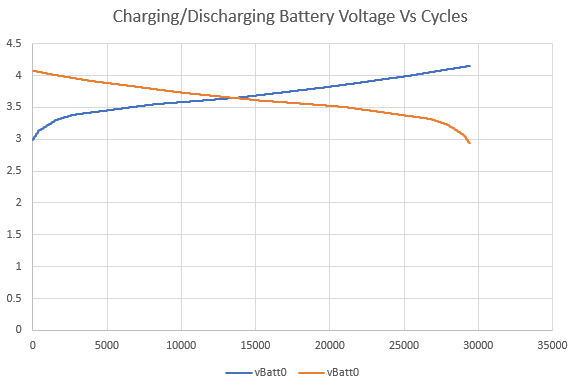
\includegraphics[scale=.5]{Chap06/Figures/Singlebatt_charge_discharge_voltage.PNG}}
% 	\qquad
% 	\subfigure[Single Battery Charging (blue)/Discharging (orange) SoC  Vs Cycles]{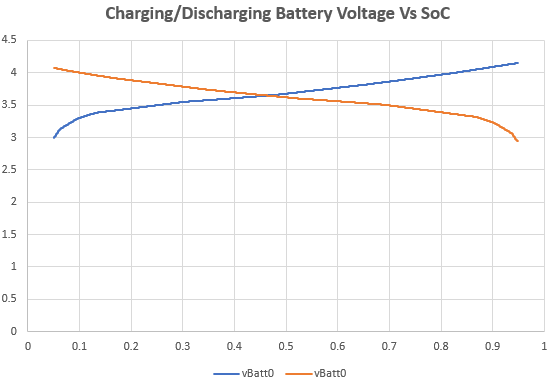
\includegraphics[scale=.5]{Chap06/Figures/Singlebatt_charge_discharge_voltage_SoC.PNG}}
% 	\qquad
% 	\subfigure[Single Battery Charging (blue)/Discharging (orange) Voltage  Vs SoC]{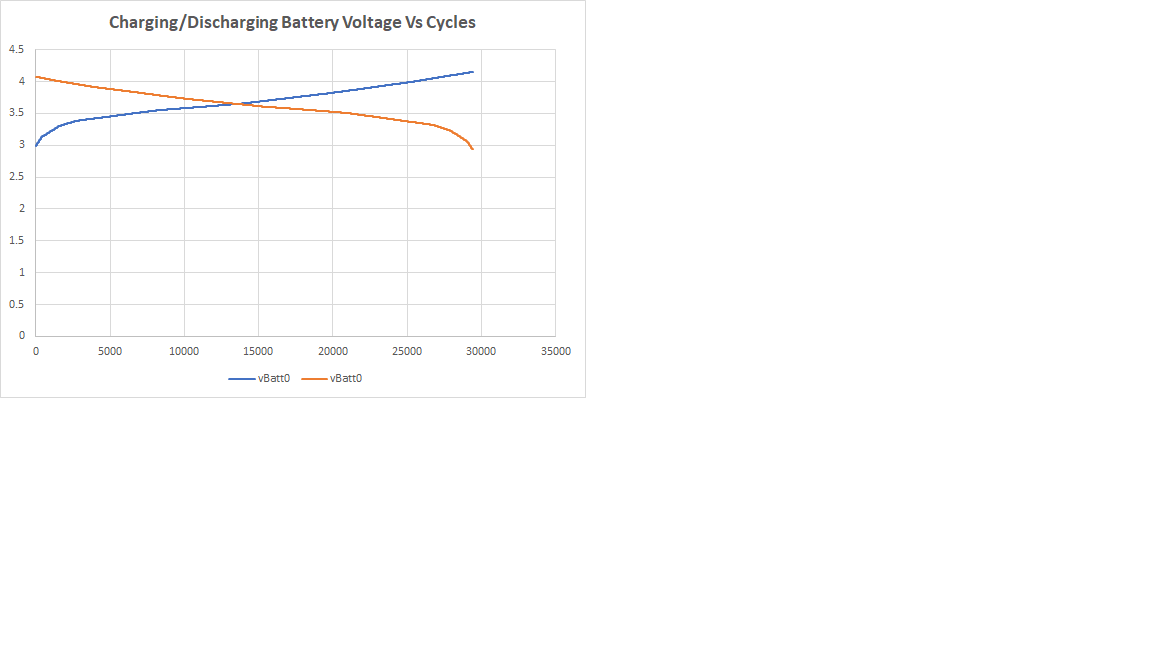
\includegraphics[scale=.5]{Chap06/Figures/Untitled.png}}
% 	\caption{Single Battery Charging and Discharging Behavior}
% 	\label{fig:Single_Batt_charge_discharge}
% \end{figure}



% \begin{tikzpicture}
%     \begin{axis}[scale only axis, xlabel = x, ylabel = y,  ytick pos=left]
%     \addplot table[x=x,y=y] {./Chap06/Code/test.xlsx};
%      \end{axis}
% \end{tikzpicture}


% % This file was created with tikzplotlib v0.10.1.
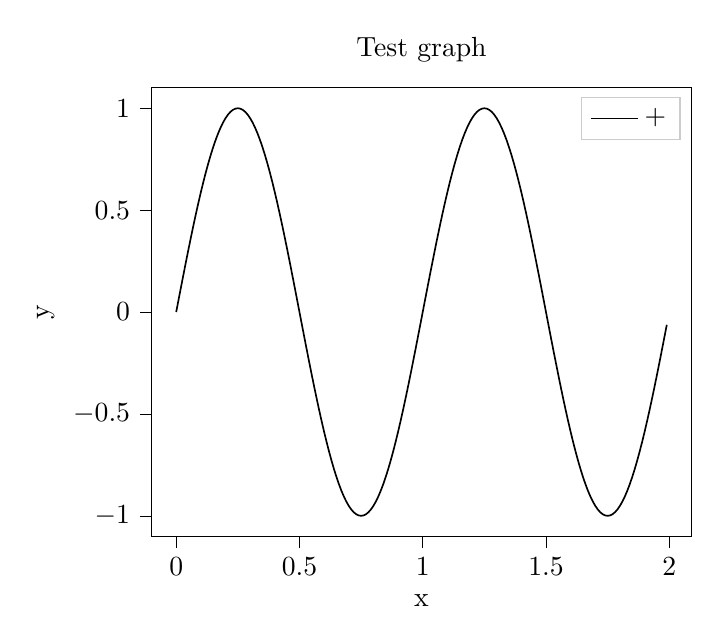
\begin{tikzpicture}

\definecolor{darkgray176}{RGB}{176,176,176}
\definecolor{lightgray204}{RGB}{204,204,204}

\begin{axis}[
legend cell align={left},
legend style={fill opacity=0.8, draw opacity=1, text opacity=1, draw=lightgray204},
tick align=outside,
tick pos=left,
title={Test graph},
x grid style={darkgray176},
xlabel={x},
xmin=-0.0995, xmax=2.0895,
xtick style={color=black},
y grid style={darkgray176},
ylabel={y},
ymin=-1.1, ymax=1.1,
ytick style={color=black}
]
\addplot [semithick, black]
table {%
0 0
0.01 0.0627905195293134
0.02 0.125333233564304
0.03 0.187381314585725
0.04 0.248689887164855
0.05 0.309016994374947
0.06 0.368124552684678
0.07 0.425779291565073
0.08 0.481753674101715
0.09 0.535826794978997
0.1 0.587785252292473
0.11 0.63742398974869
0.12 0.684547105928689
0.13 0.728968627421412
0.14 0.770513242775789
0.15 0.809016994374947
0.16 0.844327925502015
0.17 0.876306680043864
0.18 0.90482705246602
0.19 0.929776485888251
0.2 0.951056516295154
0.21 0.968583161128631
0.22 0.982287250728689
0.23 0.992114701314478
0.24 0.998026728428272
0.25 1
0.26 0.998026728428272
0.27 0.992114701314478
0.28 0.982287250728689
0.29 0.968583161128631
0.3 0.951056516295154
0.31 0.929776485888251
0.32 0.904827052466019
0.33 0.876306680043863
0.34 0.844327925502015
0.35 0.809016994374947
0.36 0.770513242775789
0.37 0.728968627421411
0.38 0.684547105928689
0.39 0.63742398974869
0.4 0.587785252292473
0.41 0.535826794978997
0.42 0.481753674101716
0.43 0.425779291565073
0.44 0.368124552684678
0.45 0.309016994374948
0.46 0.248689887164855
0.47 0.187381314585725
0.48 0.125333233564305
0.49 0.0627905195293136
0.5 1.22464679914735e-16
0.51 -0.0627905195293133
0.52 -0.125333233564304
0.53 -0.187381314585725
0.54 -0.248689887164855
0.55 -0.309016994374948
0.56 -0.368124552684678
0.57 -0.425779291565073
0.58 -0.481753674101715
0.59 -0.535826794978996
0.6 -0.587785252292473
0.61 -0.63742398974869
0.62 -0.684547105928689
0.63 -0.728968627421411
0.64 -0.770513242775789
0.65 -0.809016994374947
0.66 -0.844327925502015
0.67 -0.876306680043864
0.68 -0.90482705246602
0.69 -0.929776485888251
0.7 -0.951056516295154
0.71 -0.968583161128631
0.72 -0.982287250728689
0.73 -0.992114701314478
0.74 -0.998026728428272
0.75 -1
0.76 -0.998026728428272
0.77 -0.992114701314478
0.78 -0.982287250728689
0.79 -0.968583161128631
0.8 -0.951056516295154
0.81 -0.929776485888251
0.82 -0.90482705246602
0.83 -0.876306680043863
0.84 -0.844327925502016
0.85 -0.809016994374948
0.86 -0.77051324277579
0.87 -0.728968627421412
0.88 -0.684547105928689
0.89 -0.63742398974869
0.9 -0.587785252292473
0.91 -0.535826794978996
0.92 -0.481753674101715
0.93 -0.425779291565072
0.94 -0.368124552684678
0.95 -0.309016994374948
0.96 -0.248689887164855
0.97 -0.187381314585725
0.98 -0.125333233564305
0.99 -0.0627905195293133
1 -2.44929359829471e-16
1.01 0.0627905195293128
1.02 0.125333233564304
1.03 0.187381314585724
1.04 0.248689887164855
1.05 0.309016994374947
1.06 0.368124552684678
1.07 0.425779291565073
1.08 0.481753674101716
1.09 0.535826794978997
1.1 0.587785252292474
1.11 0.63742398974869
1.12 0.684547105928689
1.13 0.728968627421412
1.14 0.770513242775789
1.15 0.809016994374948
1.16 0.844327925502015
1.17 0.876306680043863
1.18 0.904827052466019
1.19 0.929776485888251
1.2 0.951056516295154
1.21 0.968583161128631
1.22 0.982287250728689
1.23 0.992114701314478
1.24 0.998026728428272
1.25 1
1.26 0.998026728428272
1.27 0.992114701314478
1.28 0.982287250728689
1.29 0.968583161128631
1.3 0.951056516295154
1.31 0.929776485888252
1.32 0.904827052466019
1.33 0.876306680043863
1.34 0.844327925502015
1.35 0.809016994374948
1.36 0.770513242775789
1.37 0.728968627421411
1.38 0.684547105928688
1.39 0.63742398974869
1.4 0.587785252292473
1.41 0.535826794978997
1.42 0.481753674101716
1.43 0.425779291565074
1.44 0.368124552684678
1.45 0.309016994374948
1.46 0.248689887164855
1.47 0.187381314585726
1.48 0.125333233564304
1.49 0.0627905195293134
1.5 3.67394039744206e-16
1.51 -0.0627905195293127
1.52 -0.125333233564303
1.53 -0.187381314585725
1.54 -0.248689887164855
1.55 -0.309016994374947
1.56 -0.368124552684677
1.57 -0.425779291565073
1.58 -0.481753674101716
1.59 -0.535826794978997
1.6 -0.587785252292473
1.61 -0.637423989748691
1.62 -0.684547105928689
1.63 -0.728968627421412
1.64 -0.770513242775789
1.65 -0.809016994374947
1.66 -0.844327925502016
1.67 -0.876306680043863
1.68 -0.904827052466019
1.69 -0.929776485888251
1.7 -0.951056516295153
1.71 -0.968583161128631
1.72 -0.982287250728688
1.73 -0.992114701314478
1.74 -0.998026728428272
1.75 -1
1.76 -0.998026728428272
1.77 -0.992114701314478
1.78 -0.982287250728689
1.79 -0.968583161128631
1.8 -0.951056516295154
1.81 -0.929776485888252
1.82 -0.904827052466019
1.83 -0.876306680043863
1.84 -0.844327925502015
1.85 -0.809016994374948
1.86 -0.770513242775789
1.87 -0.728968627421411
1.88 -0.684547105928689
1.89 -0.63742398974869
1.9 -0.587785252292473
1.91 -0.535826794978996
1.92 -0.481753674101716
1.93 -0.425779291565074
1.94 -0.368124552684678
1.95 -0.309016994374948
1.96 -0.248689887164856
1.97 -0.187381314585726
1.98 -0.125333233564304
1.99 -0.0627905195293135
};
\addlegendentry{+}
\end{axis}

\end{tikzpicture}

\begin{figure}[h]
    \begin{center}
        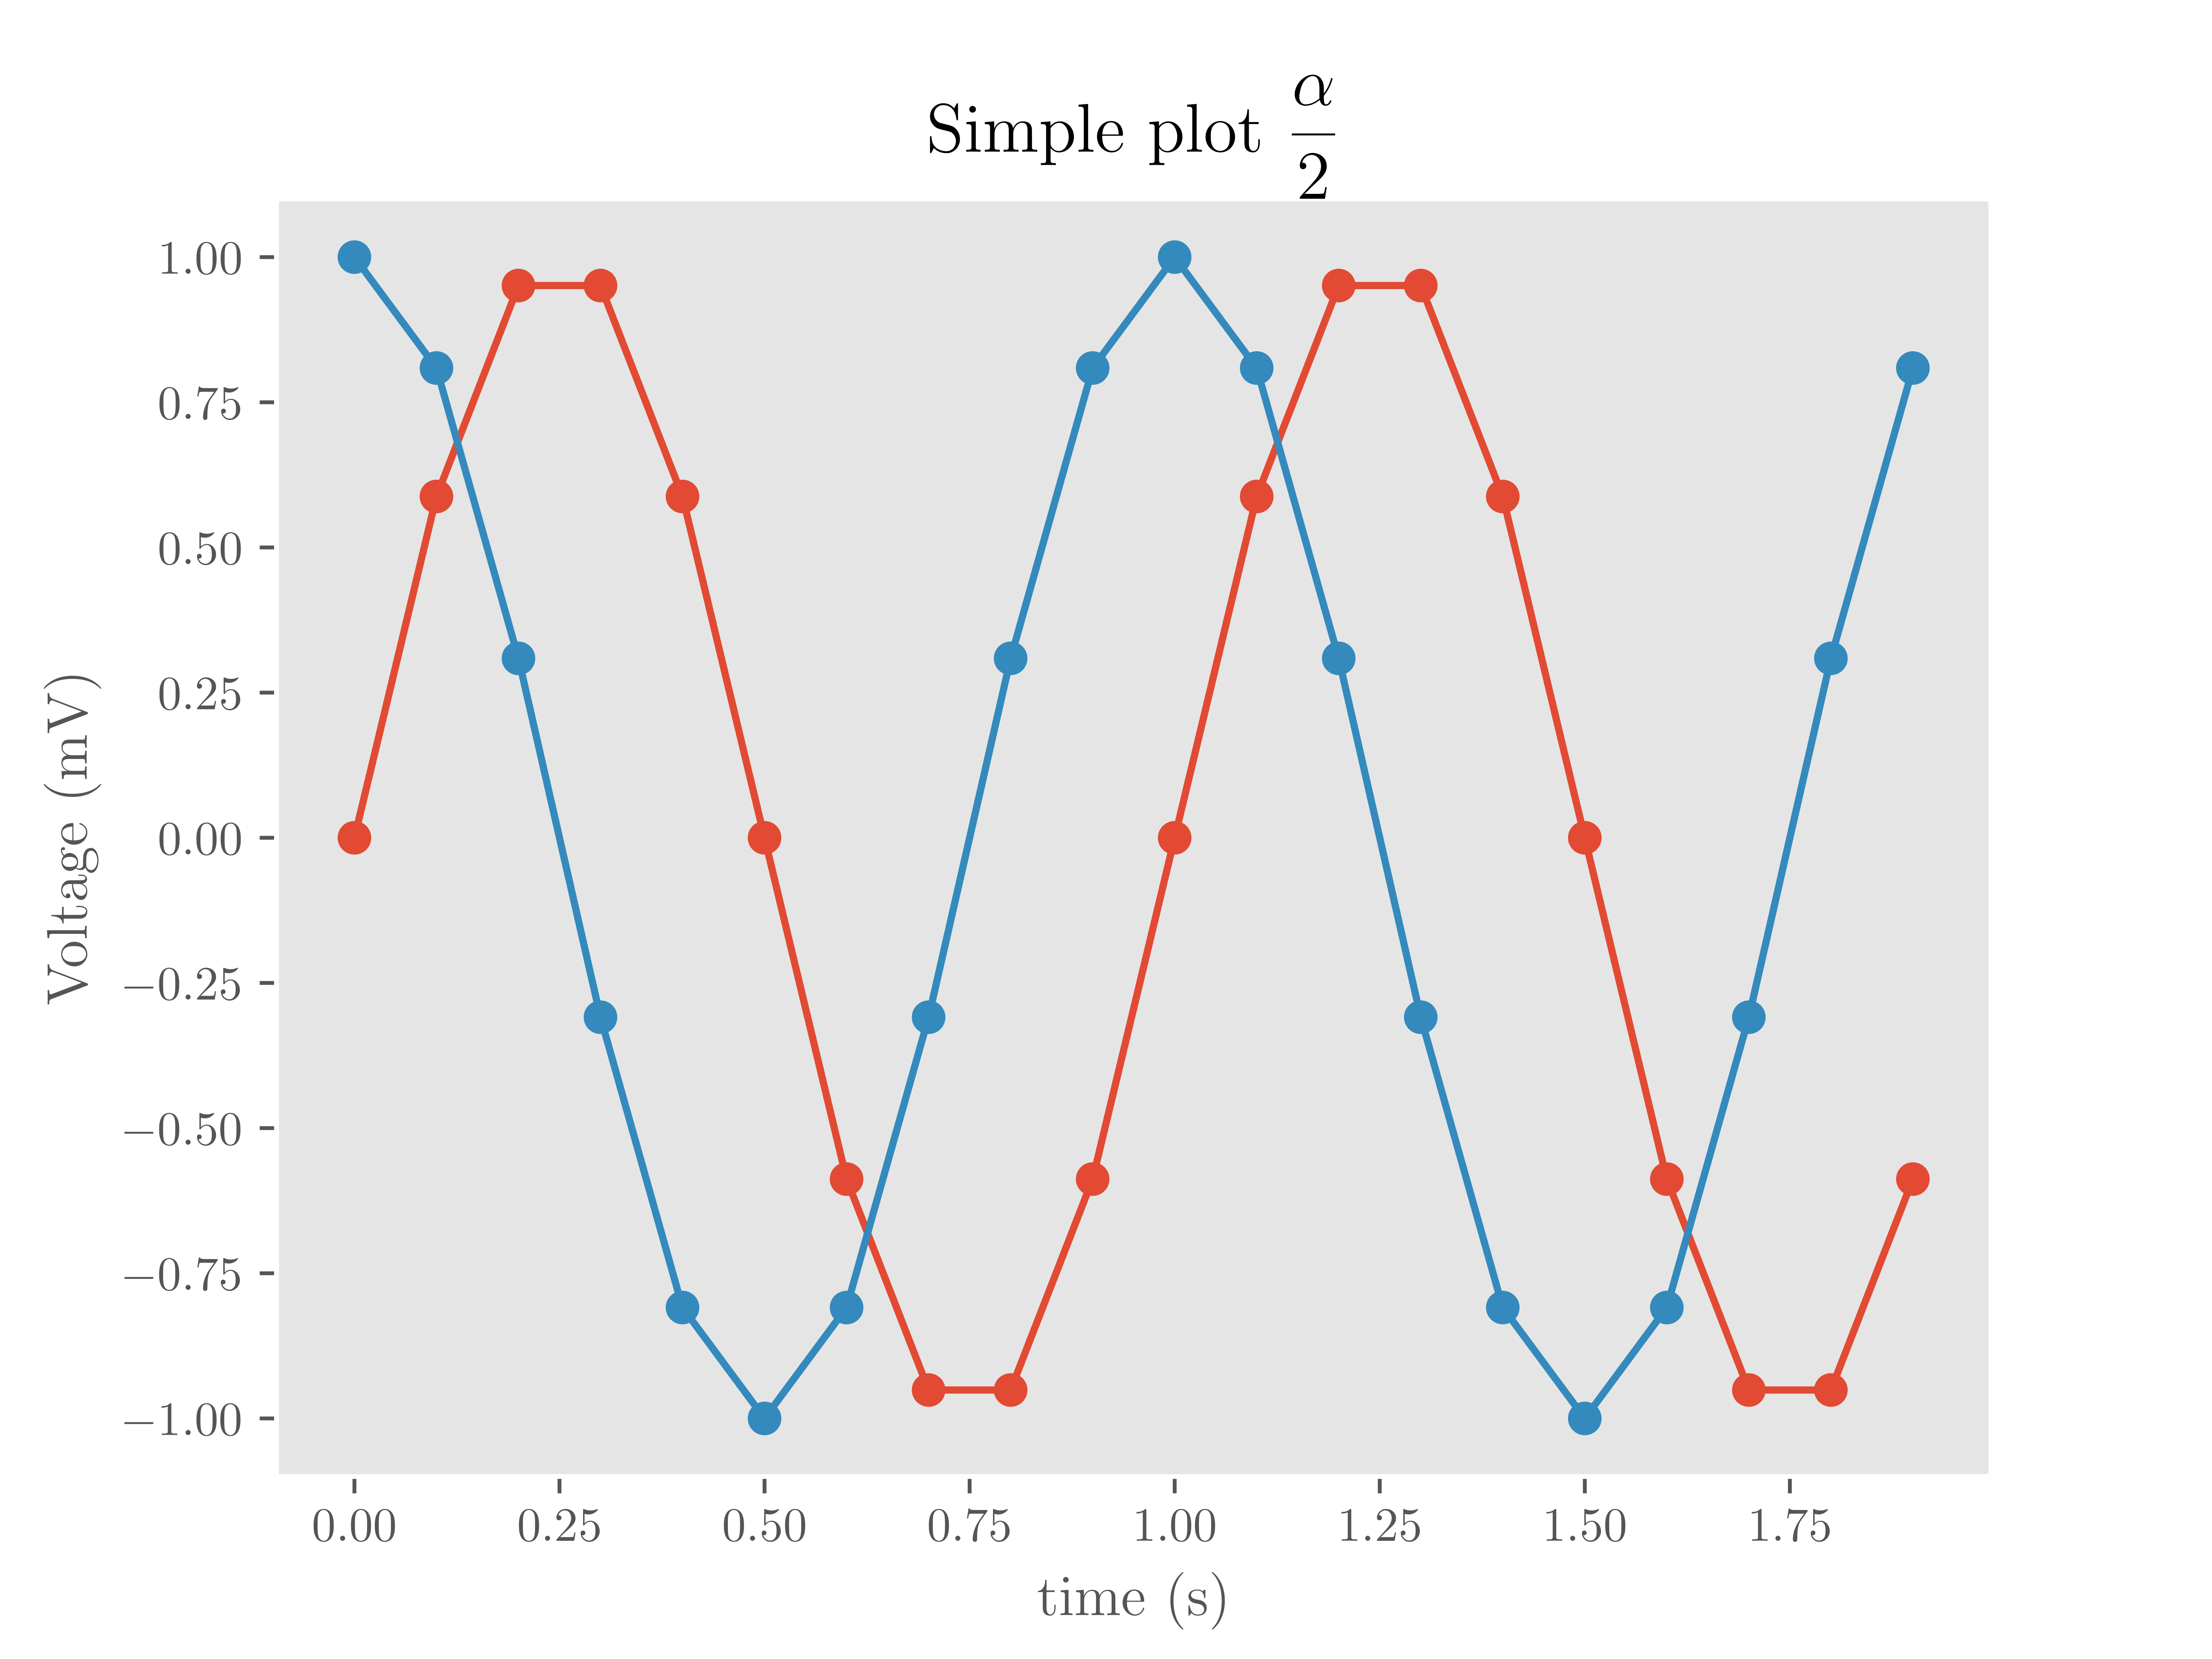
\includegraphics[width=1\textwidth]{Chap06/Code/test.png}
    \end{center}
    \caption{A PGF histogram from \texttt{matplotlib}.}
\end{figure}

% This file was created with tikzplotlib v0.10.1.

% % This file was created with tikzplotlib v0.10.1.
\begin{tikzpicture}

\definecolor{darkgray176}{RGB}{176,176,176}

\begin{axis}[
tick align=outside,
tick pos=left,
x grid style={darkgray176},
xlabel={SOC},
xmin=0.00515608004999999, xmax=0.99306651895,
xtick style={color=black},
y grid style={darkgray176},
ylabel={Voltage},
ymin=2.93560616925, ymax=4.20872189775,
ytick style={color=black}
]
\addplot [semithick, black]
table {%
0.0500611 2.993475066
0.050091649 2.993817676
0.050122199 2.994159269
0.050152749 2.994501837
0.050183299 2.994843991
0.050213848 2.995186126
0.050244398 2.995528042
0.050274948 2.995870136
0.050305499 2.996212812
0.050336049 2.996554876
0.050366598 2.99689652
0.050397148 2.997238341
0.050427698 2.997580539
0.050458248 2.997922721
0.050488797 2.998264287
0.050519347 2.998606228
0.050549896 2.99894775
0.050580446 2.999290047
0.050610996 2.99963213
0.050641546 2.999974197
0.050672095 3.00031545
0.050702645 3.000657672
0.050733194 3.000999482
0.050763745 3.001340676
0.050794295 3.001683237
0.050824845 3.002025192
0.050855395 3.002366732
0.050885944 3.002708052
0.050916494 3.003049348
0.050947043 3.003391615
0.050977592 3.003732677
0.051008142 3.004074508
0.051038691 3.00441672
0.051069241 3.004757332
0.051099791 3.005099501
0.05113034 3.005441461
0.051160891 3.005782415
0.051191441 3.006124731
0.051221991 3.006465848
0.051252541 3.006807735
0.051283091 3.007148815
0.05131364 3.007490268
0.05134419 3.007831702
0.051374739 3.008172523
0.051405289 3.008514307
0.05143584 3.008856078
0.05146639 3.009197835
0.051496939 3.009538787
0.05152749 3.009879518
0.051558039 3.010221408
0.051588588 3.010562102
0.051619138 3.010903362
0.051649688 3.011244998
0.051680238 3.011586226
0.051710788 3.01192783
0.051741337 3.012268434
0.051771887 3.012609407
0.051802437 3.01295095
0.051832987 3.013292086
0.051863536 3.013632809
0.051894086 3.013974297
0.051924636 3.01431518
0.051955186 3.014656435
0.051985736 3.014997872
0.052016286 3.015338508
0.052046836 3.015679513
0.052077385 3.0160205
0.052107935 3.016361271
0.052138484 3.016701825
0.052169033 3.017043139
0.052199584 3.017383656
0.052230133 3.017725325
0.052260682 3.018065613
0.052291232 3.018406071
0.052321782 3.018747877
0.052352332 3.019088698
0.052382882 3.019429305
0.052413432 3.019770282
0.052443982 3.020110656
0.052474532 3.020451594
0.052505082 3.020792908
0.052535631 3.021133233
0.052566181 3.021473143
0.052596731 3.021814393
0.05262728 3.022154851
0.05265783 3.022495484
0.05268838 3.022836098
0.052718928 3.023176888
0.052749478 3.023516297
0.052780028 3.023857428
0.052810578 3.024198743
0.052841128 3.024539466
0.052871678 3.024879587
0.052902228 3.025220075
0.052932778 3.025560544
0.052963328 3.025901385
0.052993878 3.026241823
0.053024428 3.026581853
0.053054977 3.026921861
0.053085527 3.027262428
0.053116076 3.027602591
0.053146626 3.027943122
0.053177176 3.028283638
0.053207726 3.028624138
0.053238275 3.028964234
0.053268825 3.029304115
0.053299376 3.029644555
0.053329926 3.029985562
0.053360475 3.030325397
0.053391024 3.030665015
0.053421574 3.031004994
0.053452123 3.031345534
0.053482672 3.031685093
0.053513222 3.032025786
0.053543771 3.032365889
0.053574321 3.03270578
0.053604871 3.033046037
0.053635421 3.033386472
0.053665971 3.033725927
0.053696521 3.034066515
0.05372707 3.03440632
0.05375762 3.034745912
0.05378817 3.035086252
0.053818719 3.035426193
0.053849268 3.035765923
0.053879818 3.03610544
0.053910368 3.036445897
0.053940918 3.036785573
0.053971467 3.037125614
0.054002017 3.037465254
0.054032566 3.037804873
0.054063116 3.038144857
0.054093666 3.038484825
0.054124216 3.038824201
0.054154765 3.039164515
0.054185315 3.039503474
0.054215864 3.039843557
0.054246414 3.040183244
0.054276964 3.040523104
0.054307514 3.040862758
0.054338064 3.041202585
0.054368614 3.041542014
0.054399164 3.041881805
0.054429713 3.042221007
0.054460263 3.042560568
0.054490813 3.042900303
0.054521363 3.043239639
0.054551912 3.04357953
0.054582462 3.04391845
0.054613012 3.044257919
0.054643562 3.044598326
0.054674112 3.044937199
0.054704662 3.04527662
0.054735212 3.045615832
0.054765762 3.045955596
0.054796311 3.046294966
0.054826861 3.046633937
0.054857411 3.046973457
0.054887961 3.047312581
0.05491851 3.047652066
0.054949059 3.047990773
0.054979609 3.048330218
0.055010159 3.048669647
0.055040709 3.04900887
0.055071259 3.049348267
0.055101808 3.049687648
0.055132358 3.050026062
0.055162908 3.05036597
0.055193457 3.05070511
0.055224007 3.051043472
0.055254556 3.051383135
0.055285106 3.051721839
0.055315655 3.052060709
0.055346205 3.052400318
0.055376754 3.052738778
0.055407304 3.053077972
0.055437855 3.053417719
0.055468405 3.05375689
0.055498955 3.054095478
0.055529504 3.054434421
0.055560054 3.05477278
0.055590603 3.05511187
0.055621153 3.055450567
0.055651702 3.055789243
0.055682252 3.056128089
0.055712802 3.056467484
0.055743352 3.056806681
0.055773902 3.057145299
0.055804452 3.057483897
0.055835001 3.057822475
0.05586555 3.058160655
0.0558961 3.058500131
0.05592665 3.058838657
0.055957199 3.059177351
0.055987749 3.059516029
0.056018298 3.0598545
0.056048848 3.06019314
0.056079397 3.060532138
0.056109947 3.060870183
0.056140497 3.061209332
0.056171047 3.061548096
0.056201597 3.061886656
0.056232147 3.06222501
0.056262697 3.062563345
0.056293247 3.062902786
0.056323797 3.063240345
0.056354347 3.063579188
0.056384897 3.06391708
0.056415447 3.064256634
0.056445996 3.064594125
0.056476545 3.064932147
0.056507094 3.065270334
0.056537645 3.065609063
0.056568194 3.065947967
0.056598744 3.066286113
0.056629293 3.066624052
0.056659842 3.066962155
0.056690392 3.067300613
0.056720942 3.067639055
0.056751492 3.067977296
0.056782042 3.068315707
0.056812591 3.068654103
0.05684314 3.068991365
0.05687369 3.069329902
0.056904239 3.069668428
0.056934789 3.070006382
0.056965338 3.070344316
0.056995889 3.070682603
0.057026439 3.071021062
0.057056989 3.071359137
0.057087539 3.071697194
0.057118089 3.072035234
0.057148639 3.072373071
0.057179189 3.07271126
0.057209738 3.073049062
0.057240288 3.073386845
0.057270839 3.073724979
0.057301388 3.074063285
0.057331937 3.07440065
0.057362486 3.07473799
0.057393036 3.075076233
0.057423586 3.075414279
0.057454136 3.075752495
0.057484686 3.076090143
0.057515236 3.076428143
0.057545785 3.076765572
0.057576335 3.07710335
0.057606885 3.077441295
0.057637435 3.077779041
0.057667986 3.078116771
0.057698535 3.078455038
0.057729085 3.078792002
0.057759635 3.079129678
0.057790185 3.079467337
0.057820735 3.079805718
0.057851285 3.080142985
0.057881834 3.080480045
0.057912383 3.080817449
0.057942934 3.081155387
0.057973484 3.081493681
0.058004034 3.081831047
0.058034584 3.082168394
0.058065134 3.082505352
0.058095683 3.082843206
0.058126233 3.083180496
0.058156783 3.083517951
0.058187332 3.083855388
0.058217882 3.084192809
0.058248432 3.08453058
0.058278981 3.084867788
0.058309531 3.085204243
0.058340081 3.08554287
0.05837063 3.08587948
0.058401181 3.08621698
0.05843173 3.086554833
0.058462279 3.086891211
0.058492829 3.087228475
0.058523379 3.087566271
0.058553928 3.087903509
0.058584478 3.088240365
0.058615028 3.088578113
0.058645578 3.08891512
0.058676128 3.089252109
0.058706676 3.089589626
0.058737226 3.089925669
0.058767776 3.090263324
0.058798326 3.090601153
0.058828876 3.090938245
0.058859426 3.09127459
0.058889975 3.091612186
0.058920525 3.091948131
0.058951074 3.092286231
0.058981624 3.09262269
0.059012173 3.092960036
0.059042722 3.093296278
0.059073272 3.093633767
0.059103821 3.093970337
0.059134371 3.094307796
0.05916492 3.094644518
0.05919547 3.094981221
0.05922602 3.095317905
0.059256569 3.095655478
0.059287119 3.095991955
0.059317668 3.096328592
0.059348218 3.096665391
0.059378767 3.097002174
0.059409317 3.097339303
0.059439867 3.097675877
0.059470417 3.098012612
0.059500966 3.098349513
0.059531516 3.098686217
0.059562066 3.099022905
0.059592615 3.099359396
0.059623165 3.099695867
0.059653715 3.10003286
0.059684265 3.10036948
0.059714814 3.100705903
0.059745364 3.101042306
0.059775914 3.10137923
0.059806463 3.101715963
0.059837013 3.102051959
0.059867563 3.102388653
0.059898113 3.102725154
0.059928663 3.103062179
0.059959213 3.103398296
0.059989762 3.103734933
0.060020312 3.104070657
0.060050861 3.104407617
0.06008141 3.104743311
0.060111959 3.10507988
0.060142509 3.105416438
0.060173059 3.105752804
0.060203609 3.106089512
0.060234158 3.106426208
0.060264708 3.106761813
0.060295258 3.107098106
0.060325808 3.107434737
0.060356357 3.107770992
0.060386907 3.108106865
0.060417456 3.108443245
0.060448005 3.108779245
0.060478554 3.109115036
0.060509103 3.109451158
0.060539652 3.109787262
0.060570202 3.110123889
0.060600751 3.110460158
0.0606313 3.110795708
0.060661849 3.111131609
0.060692399 3.111467868
0.060722949 3.111804495
0.060753499 3.112140786
0.060784049 3.112476384
0.060814599 3.112813064
0.060845149 3.113149051
0.060875698 3.113485389
0.060906248 3.113821174
0.060936799 3.114157452
0.060967349 3.114494035
0.060997899 3.114829488
0.061028449 3.11516556
0.061058999 3.115501353
0.061089548 3.115836673
0.061120098 3.116172207
0.061150647 3.116507768
0.061181197 3.116842658
0.061211747 3.117177636
0.061242296 3.117513654
0.061272846 3.117848126
0.061303396 3.118183752
0.061333945 3.118518834
0.061364494 3.118854487
0.061395044 3.119190424
0.061425593 3.119526881
0.061456144 3.119863393
0.061486693 3.120201254
0.061517243 3.120538375
0.061547793 3.120876163
0.061578343 3.121214924
0.061608893 3.121552853
0.061639443 3.121890064
0.061669993 3.122226853
0.061700543 3.12256335
0.061731093 3.122898449
0.061761643 3.123232272
0.061792192 3.12356406
0.061822741 3.123894459
0.06185329 3.124223103
0.06188384 3.124550356
0.06191439 3.124877232
0.06194494 3.125203533
0.06197549 3.125530804
0.062006039 3.125860248
0.062036588 3.126191667
0.062067138 3.126527308
0.062097687 3.126867332
0.062128236 3.12721206
0.062158786 3.127563217
0.062189336 3.127921654
0.062219885 3.12828639
0.062250434 3.12865494
0.062280984 3.129023599
0.062311534 3.129390938
0.062342084 3.129752041
0.062372634 3.130103897
0.062403184 3.130443675
0.062433733 3.13076872
0.062464283 3.131074463
0.062494832 3.131359636
0.062525382 3.13161863
0.062555932 3.131851997
0.062586482 3.132058642
0.062617031 3.132242252
0.062647581 3.132406524
0.062678131 3.132555154
0.062708681 3.13268994
0.06273923 3.132814576
0.06276978 3.132932928
0.06280033 3.133047659
0.06283088 3.133161774
0.062861429 3.133278795
0.062891979 3.133400797
0.062922529 3.133530943
0.062953079 3.133667459
0.062983628 3.133808807
0.063014177 3.133955169
0.063044727 3.134105008
0.063075277 3.134258681
0.063105827 3.134413794
0.063136377 3.134570528
0.063166927 3.134727693
0.063197476 3.13488444
0.063228026 3.135038889
0.063258575 3.135192656
0.063289125 3.135343599
0.063319674 3.135494506
0.063350224 3.135643026
0.063380773 3.135790398
0.063411323 3.135937181
0.063441873 3.13608325
0.063472422 3.136228651
0.063502971 3.136373425
0.063533522 3.136518301
0.063564071 3.136664181
0.063594621 3.136809216
0.06362517 3.136955344
0.063655719 3.13710153
0.063686268 3.13724827
0.063716818 3.137395039
0.063747368 3.137543019
0.063777918 3.137691004
0.063808467 3.13783915
0.063839016 3.137987273
0.063869566 3.138136037
0.063900116 3.138284922
0.063930666 3.138435104
0.063961215 3.138584525
0.063991765 3.138733658
0.064022315 3.138884343
0.064052865 3.139034512
0.064083415 3.139184471
0.064113965 3.139335206
0.064144514 3.139485329
0.064175064 3.139635826
0.064205614 3.139786326
0.064236164 3.139936797
0.064266714 3.140087719
0.064297264 3.140237709
0.064327814 3.140388295
0.064358363 3.140537788
0.064388913 3.14068823
0.064419463 3.140838108
0.064450013 3.140988106
0.064480563 3.141138232
0.064511112 3.141288329
0.064541662 3.141437724
0.064572211 3.141587779
0.06460276 3.141737491
0.06463331 3.141887372
0.06466386 3.142037257
0.06469441 3.142187821
0.06472496 3.142337373
0.064755509 3.142487088
0.064786058 3.142636797
0.064816609 3.142786667
0.064847159 3.142937035
0.064877708 3.143086886
0.064908258 3.143236383
0.064938806 3.143386031
0.064969356 3.143535152
0.064999906 3.143685938
0.065030456 3.143835528
0.065061006 3.143985604
0.065091555 3.144135157
0.065122105 3.144284353
0.065152654 3.144434541
0.065183204 3.14458421
0.065213754 3.144733863
0.065244304 3.144883331
0.065274854 3.145033121
0.065305403 3.145182898
0.065335954 3.145331988
0.065366504 3.14548241
0.065397053 3.145631475
0.065427604 3.145780692
0.065458153 3.145930903
0.065488702 3.146079588
0.065519252 3.146229263
0.065549801 3.146379262
0.065580351 3.14652807
0.065610901 3.146678205
0.065641451 3.14682732
0.065672 3.14697709
0.06570255 3.147125838
0.0657331 3.147275574
0.065763649 3.147425297
0.065794199 3.147574167
0.065824748 3.147723691
0.065855298 3.147872864
0.065885847 3.148022021
0.065916397 3.148171499
0.065946946 3.14832113
0.065977496 3.148470077
0.066008046 3.148619847
0.066038595 3.148768934
0.066069145 3.14891767
0.066099694 3.149067394
0.066130245 3.149216102
0.066160794 3.149366131
0.066191343 3.149514477
0.066221893 3.149663973
0.066252443 3.14981329
0.066282993 3.149962259
0.066313543 3.150111378
0.066344093 3.150261152
0.066374642 3.150409577
0.066405192 3.150558484
0.066435742 3.150708043
0.066466292 3.150856755
0.066496841 3.151005784
0.066527391 3.151154966
0.066557941 3.151303966
0.066588491 3.151453119
0.06661904 3.151601591
0.06664959 3.151750546
0.06668014 3.151899485
0.06671069 3.152049245
0.066741238 3.152197328
0.066771788 3.152345891
0.066802338 3.152495437
0.066832887 3.15264414
0.066863437 3.152792828
0.066893987 3.152941999
0.066924537 3.153090991
0.066955086 3.153239304
0.066985635 3.153387931
0.067016185 3.153537042
0.067046735 3.153685474
0.067077284 3.153834721
0.067107833 3.153982959
0.067138383 3.154131843
0.067168933 3.154281213
0.067199482 3.154429077
0.067230031 3.154578083
0.067260581 3.154726413
0.067291131 3.15487539
0.067321681 3.155024023
0.067352231 3.155172974
0.06738278 3.15532158
0.06741333 3.155469841
0.067443879 3.155618085
0.067474429 3.155766975
0.067504978 3.155915688
0.067535528 3.15606389
0.067566077 3.156212572
0.067596628 3.15636091
0.067627177 3.156510059
0.067657727 3.156658041
0.067688276 3.1568065
0.067718827 3.156954779
0.067749376 3.157103704
0.067779927 3.157251956
0.067810476 3.157400523
0.067841027 3.157548746
0.067871576 3.157697284
0.067902126 3.157845312
0.067932676 3.157993819
0.067963226 3.158141983
0.067993775 3.158290627
0.068024325 3.158438268
0.068054874 3.158587375
0.068085424 3.158734825
0.068115973 3.158883244
0.068146522 3.159031156
0.068177071 3.159179876
0.068207622 3.15932776
0.068238171 3.159476617
0.068268721 3.159624476
0.06829927 3.159772977
0.06832982 3.159920478
0.068360369 3.160068619
0.068390919 3.160217074
0.068421468 3.160365187
0.068452017 3.160512957
0.068482567 3.160660874
0.068513116 3.160809432
0.068543666 3.160957158
0.068574215 3.161105688
0.068604765 3.161253386
0.068635315 3.161402053
0.068665865 3.16154956
0.068696415 3.161698035
0.068726964 3.161845679
0.068757514 3.161993144
0.068788064 3.162141575
0.068818614 3.162289833
0.068849163 3.162436933
0.068879713 3.162585326
0.068910262 3.162732891
0.068940811 3.162880441
0.068971361 3.163028795
0.069001911 3.163176649
0.069032461 3.163324491
0.06906301 3.163472485
0.06909356 3.163620304
0.06912411 3.163767947
0.06915466 3.163915741
0.06918521 3.164063686
0.06921576 3.16421162
0.069246309 3.16435938
0.069276859 3.164506474
0.069307408 3.164654532
0.069337958 3.164802417
0.069368507 3.164949965
0.069399058 3.1650975
0.069429608 3.165245674
0.069460157 3.165393351
0.069490707 3.16554069
0.069521257 3.165688341
0.069551807 3.165836307
0.069582356 3.165983611
0.069612906 3.16613139
0.069643456 3.166278833
0.069674005 3.166426426
0.069704555 3.166573681
0.069735104 3.166721899
0.069765654 3.166868971
0.069796204 3.167016678
0.069826754 3.167164374
0.069857304 3.167311897
0.069887854 3.167459734
0.069918404 3.167607074
0.069948954 3.167754238
0.069979504 3.167901875
0.070010053 3.168049339
0.070040603 3.16819663
0.070071153 3.168344394
0.070101702 3.168491501
0.070132252 3.168638268
0.070162801 3.168786804
0.070193351 3.168933553
0.0702239 3.169080934
0.07025445 3.169228303
0.070285001 3.16937631
0.07031555 3.169523661
0.0703461 3.169670516
0.070376648 3.169817679
0.070407198 3.169964507
0.070437747 3.170112291
0.070468297 3.170259744
0.070498847 3.170407025
0.070529396 3.170554295
0.070559946 3.170701554
0.070590496 3.170848478
0.070621045 3.170996359
0.070651595 3.171143262
0.070682144 3.171290313
0.070712694 3.171437673
0.070743244 3.171585022
0.070773794 3.171732037
0.070804344 3.171879521
0.070834894 3.17202651
0.070865443 3.172173968
0.070895993 3.172320448
0.070926542 3.172467394
0.070957092 3.17261465
0.070987642 3.172761896
0.071018191 3.172909134
0.071048741 3.173055882
0.071079292 3.173203586
0.071109842 3.173350645
0.071140391 3.173497538
0.071170941 3.173644105
0.071201491 3.17379147
0.071232041 3.173938674
0.07126259 3.174085554
0.07129314 3.174232103
0.07132369 3.1743796
0.07135424 3.174526603
0.07138479 3.174673905
0.07141534 3.174820222
0.071445889 3.174967628
0.071476439 3.17511388
0.071506989 3.175261374
0.071537539 3.175407869
0.071568089 3.175555117
0.071598639 3.175701524
0.071629188 3.175848221
0.071659738 3.175994906
0.071690288 3.176141435
0.071720838 3.176288301
0.071751387 3.176435045
0.071781937 3.176581519
0.071812487 3.176728698
0.071843037 3.176875802
0.071873587 3.177022525
0.071904137 3.17717
0.071934686 3.177316964
0.071965236 3.177464363
0.071995786 3.177612026
0.072026336 3.17775994
0.072056884 3.177906815
0.072087434 3.178054227
0.072117984 3.178202643
0.072148534 3.17835078
0.072179084 3.178498623
0.072209634 3.178646155
0.072240184 3.178794317
0.072270734 3.178942303
0.072301284 3.17908947
0.072331833 3.179237885
0.072362382 3.179384849
0.072392931 3.179532267
0.072423481 3.179680621
0.072454032 3.179828645
0.072484581 3.179976497
0.07251513 3.180123382
0.07254568 3.180270887
0.07257623 3.180419494
0.072606779 3.180566669
0.072637329 3.180714309
0.072667878 3.180861783
0.072698428 3.181009566
0.072728978 3.181157342
0.072759528 3.181304793
0.072790077 3.181452869
0.072820627 3.181599668
0.072851176 3.181747563
0.072881726 3.181894974
0.072912275 3.182042373
0.072942825 3.182190236
0.072973375 3.182337773
0.073003924 3.182485299
0.073034474 3.182632972
0.073065024 3.182780477
0.073095574 3.182927812
0.073126124 3.183075293
0.073156673 3.183223081
0.073187222 3.183370067
0.073217772 3.183517198
0.073248323 3.183665584
0.073278872 3.183813174
0.073309422 3.183959804
0.073339972 3.184107684
0.073370522 3.184254766
0.073401071 3.184402152
0.073431621 3.184549686
0.07346217 3.184696895
0.07349272 3.184844091
0.07352327 3.184991751
0.07355382 3.185139086
0.07358437 3.185286569
0.07361492 3.185433885
0.07364547 3.185581032
0.07367602 3.185728325
0.07370657 3.185875451
0.07373712 3.186023196
0.073767669 3.18616983
0.073798219 3.186317395
0.073828769 3.186464479
0.073859319 3.186612025
0.073889868 3.186758774
0.073920417 3.186905825
0.073950967 3.187053337
0.073981517 3.187200526
0.074012065 3.187347704
0.074042615 3.187494399
0.074073164 3.187641711
0.074103715 3.187789329
0.074134265 3.187936782
0.074164814 3.188083598
0.074195364 3.188230559
0.074225914 3.188377823
0.074256464 3.188524764
0.074287014 3.188672323
0.074317564 3.188818774
0.074348114 3.188966311
0.074378664 3.189113213
0.074409213 3.189260419
0.074439763 3.189407144
0.074470312 3.189554171
0.074500862 3.189701031
0.074531411 3.189848036
0.07456196 3.189994717
0.07459251 3.190142015
0.07462306 3.190289147
0.074653609 3.190436584
0.074684158 3.190582759
0.074714708 3.19072986
0.074745258 3.190877108
0.074775808 3.191024034
0.074806357 3.191170637
0.074836907 3.191317541
0.074867457 3.191465062
0.074898007 3.191611637
0.074928557 3.191758514
0.074959106 3.191905537
0.074989655 3.192051611
0.075020205 3.192198765
0.075050755 3.192345756
0.075081305 3.192492894
0.075111855 3.192639711
0.075142406 3.192786519
0.075172955 3.192933317
0.075203504 3.193079479
0.075234054 3.193226566
0.075264604 3.193373175
0.075295153 3.1935204
0.075325703 3.193666523
0.075356253 3.19381357
0.075386802 3.19396061
0.075417352 3.194106862
0.075447902 3.194254037
0.075478451 3.194400425
0.075509001 3.194547114
0.075539551 3.194693793
0.0755701 3.194840461
0.07560065 3.194986965
0.075631201 3.195134081
0.07566175 3.195281034
0.0756923 3.195427045
0.075722849 3.195573509
0.075753399 3.195720273
0.075783949 3.195866872
0.075814499 3.196013774
0.075845049 3.196160045
0.075875599 3.19630677
0.075906149 3.196453643
0.075936698 3.196599886
0.075967248 3.196746117
0.075997798 3.196892958
0.076028348 3.19703917
0.076058898 3.197186459
0.076089448 3.197332344
0.076119998 3.197479459
0.076150548 3.197625637
0.076181098 3.197771647
0.076211648 3.197918421
0.076242197 3.198064877
0.076272747 3.198210858
0.076303297 3.198358068
0.076333847 3.198504032
0.076364396 3.198650759
0.076394945 3.198796393
0.076425495 3.198942942
0.076456045 3.199089948
0.076486595 3.199236174
0.076517145 3.199382544
0.076547695 3.19952906
0.076578246 3.199675722
0.076608797 3.199821912
0.076639347 3.199968557
0.076669897 3.20011442
0.076700447 3.20026058
0.076730996 3.20040704
0.076761547 3.200553026
0.076792096 3.200699775
0.076822646 3.20084559
0.076853196 3.200991856
0.076883745 3.201138268
0.076914294 3.201283898
0.076944843 3.201430287
0.076975392 3.201576359
0.077005942 3.201723039
0.077036492 3.201869403
0.077067042 3.20201576
0.077097592 3.202161644
0.077128141 3.202307826
0.07715869 3.202453843
0.07718924 3.202599696
0.077219789 3.202746462
0.077250339 3.202892453
0.077280889 3.203038741
0.077311439 3.203185022
0.077341989 3.203330985
0.077372538 3.203476939
0.077403089 3.203623036
0.077433638 3.203769586
0.077464188 3.203915206
0.077494737 3.204061122
0.077525285 3.204207027
0.077555835 3.204352614
0.077586385 3.204499574
0.077616935 3.204645763
0.077647485 3.204791635
0.077678034 3.204937498
0.077708585 3.205083504
0.077739134 3.205229962
0.077769683 3.205375184
0.077800233 3.205521314
0.077830782 3.205667128
0.077861332 3.205813085
0.077891882 3.205959495
0.077922432 3.206105591
0.077952981 3.206251526
0.077983531 3.206396838
0.07801408 3.206543057
0.078044631 3.206689116
0.07807518 3.206835321
0.07810573 3.206980446
0.07813628 3.207126936
0.07816683 3.207272962
0.078197379 3.207418213
0.078227929 3.207563911
0.078258478 3.207710212
0.078289028 3.207855894
0.078319578 3.208001873
0.078350128 3.208147845
0.078380678 3.208293348
0.078411228 3.208439607
0.078441778 3.208585247
0.078472328 3.208730724
0.078502877 3.208876496
0.078533426 3.209021799
0.078563975 3.209167855
0.078594525 3.209313598
0.078625075 3.209459638
0.078655625 3.209605213
0.078686175 3.209751084
0.078716726 3.209897252
0.078747275 3.210042803
0.078777825 3.21018804
0.078808375 3.210333721
0.078838925 3.2104797
0.078869475 3.210625061
0.078900025 3.210771021
0.078930574 3.210916517
0.078961125 3.211062156
0.078991674 3.211207939
0.079022224 3.211353104
0.079052773 3.211498866
0.079083323 3.211644317
0.079113872 3.211790214
0.079144421 3.211935344
0.079174971 3.212081071
0.07920552 3.212226485
0.07923607 3.212372347
0.079266619 3.212518051
0.07929717 3.21266329
0.079327719 3.21280928
0.079358269 3.212954655
0.079388819 3.213100021
0.079419369 3.213245682
0.079449918 3.213391335
0.079480468 3.213536372
0.079511018 3.213682005
0.079541567 3.213827479
0.079572117 3.213972792
0.079602666 3.214118703
0.079633215 3.214263545
0.079663765 3.214408982
0.079694314 3.214554864
0.079724864 3.214699832
0.079755414 3.214845697
0.079785963 3.214990798
0.079816513 3.21513604
0.079847062 3.215282029
0.079877613 3.215426954
0.079908162 3.215572926
0.079938712 3.215717834
0.079969262 3.215863336
0.079999812 3.216008527
0.080030362 3.216154164
0.080060912 3.216299189
0.080091462 3.21644496
0.080122011 3.21658982
0.080152561 3.216735123
0.080183112 3.216880721
0.080213662 3.217026163
0.080244211 3.217171298
0.080274761 3.217316122
0.080305311 3.217461842
0.08033586 3.217606802
0.08036641 3.217752052
0.08039696 3.217897444
0.08042751 3.218042524
0.08045806 3.218187742
0.080488609 3.21833325
0.080519159 3.218478143
0.080549708 3.218623171
0.080580257 3.218768183
0.080610807 3.218913329
0.080641357 3.219058764
0.080671906 3.219204191
0.080702455 3.21934886
0.080733004 3.219493822
0.080763554 3.219638934
0.080794104 3.219784501
0.080824653 3.219929474
0.080855204 3.220074455
0.080885754 3.220220199
0.080916303 3.220365061
0.080946854 3.220510239
0.080977403 3.22065559
0.081007953 3.220800665
0.081038504 3.220946067
0.081069053 3.22109135
0.081099603 3.221236215
0.081130152 3.221381864
0.081160702 3.221527103
0.081191252 3.221672533
0.081221802 3.221818157
0.081252351 3.221963531
0.081282901 3.222109253
0.081313451 3.222254578
0.081344001 3.222400696
0.081374551 3.222546107
0.0814051 3.222692147
0.081435649 3.222837315
0.0814662 3.222983396
0.081496749 3.223129492
0.081527299 3.223275145
0.081557849 3.223420945
0.081588399 3.223566735
0.081618948 3.223712211
0.081649498 3.223858261
0.081680047 3.224003542
0.081710597 3.224149397
0.081741146 3.224295533
0.081771696 3.224440757
0.081802245 3.22458641
0.081832795 3.2247316
0.081863345 3.224878421
0.081893894 3.225023445
0.081924444 3.225169054
0.081954993 3.225314507
0.081985543 3.225460252
0.082016092 3.225605696
0.082046642 3.225751283
0.082077191 3.225897165
0.082107741 3.226042446
0.08213829 3.226188316
0.082168841 3.226333436
0.08219939 3.22647989
0.08222994 3.226624402
0.08226049 3.226770541
0.082291041 3.226916378
0.08232159 3.227061911
0.08235214 3.227207136
0.08238269 3.227352649
0.082413239 3.227497855
0.082443789 3.227643198
0.082474339 3.227789279
0.082504888 3.22793461
0.082535439 3.228079931
0.082565989 3.22822599
0.082596539 3.22837115
0.082627089 3.228516747
0.082657639 3.228661593
0.082688189 3.228807469
0.082718738 3.228953044
0.082749288 3.229097718
0.082779838 3.229243422
0.082810388 3.22938912
0.082840937 3.229534068
0.082871487 3.229679749
0.082902037 3.229825127
0.082932587 3.229970646
0.082963136 3.230115713
0.082993687 3.230260917
0.083024236 3.230406708
0.083054786 3.23055175
0.083085337 3.230697526
0.083115886 3.230842703
0.083146436 3.230987722
0.083176985 3.231133028
0.083207535 3.231278326
0.083238084 3.231423617
0.083268634 3.231568602
0.083299183 3.231714172
0.083329734 3.231859292
0.083360283 3.232005144
0.083390833 3.232149807
0.083421383 3.232295496
0.083451933 3.232440587
0.083482482 3.23258567
0.083513031 3.232730893
0.08354358 3.232875515
0.083574129 3.233021162
0.08360468 3.233166213
0.083635229 3.233311996
0.083665779 3.233456887
0.083696328 3.233601916
0.083726878 3.233747381
0.083757427 3.233892397
0.083787976 3.234037107
0.083818526 3.234182547
0.083849076 3.234327834
0.083879625 3.234473114
0.083910175 3.234618092
0.083940725 3.234763209
0.083971274 3.234908467
0.084001824 3.235053274
0.084032374 3.235198515
0.084062924 3.235343601
0.084093473 3.235488976
0.084124023 3.235633459
0.084154573 3.235779111
0.084185122 3.235924022
0.084215672 3.236068629
0.084246221 3.236213963
0.084276771 3.236358849
0.084307321 3.236504317
0.084337871 3.236649191
0.08436842 3.236794352
0.08439897 3.236938916
0.08442952 3.237084059
0.084460071 3.237229492
0.08449062 3.237374331
0.08452117 3.237518866
0.08455172 3.237664276
0.08458227 3.237809092
0.084612819 3.237953899
0.08464337 3.238098846
0.084673919 3.238244227
0.084704469 3.238388868
0.084735019 3.238533499
0.084765568 3.23867871
0.084796118 3.238823474
0.084826668 3.238968229
0.084857218 3.23911386
0.084887767 3.239258164
0.084918317 3.239402897
0.084948866 3.239547769
0.084979416 3.239692781
0.085009966 3.239837934
0.085040516 3.239982346
0.085071066 3.240127482
0.085101616 3.240272467
0.085132165 3.240417151
0.085162715 3.240561826
0.085193265 3.240706934
0.085223814 3.240851449
0.085254364 3.240996102
0.085284914 3.241141186
0.085315464 3.241286119
0.085346014 3.2414309
0.085376564 3.241575526
0.085407114 3.241720291
0.085437664 3.241865195
0.085468213 3.242009508
0.085498763 3.242154102
0.085529313 3.242299276
0.085559862 3.242444152
0.085590411 3.242588144
0.085620961 3.242733295
0.085651511 3.242878003
0.08568206 3.243022704
0.08571261 3.243167544
0.08574316 3.243312085
0.08577371 3.243456911
0.08580426 3.243601878
0.08583481 3.243746255
0.085865359 3.243890768
0.085895909 3.244035126
0.085926459 3.2441805
0.085957008 3.244324556
0.085987557 3.244469038
0.086018107 3.244613805
0.086048657 3.244758565
0.086079206 3.24490332
0.086109756 3.24504763
0.086140306 3.245192515
0.086170855 3.245336958
0.086201404 3.245481538
0.086231954 3.245625672
0.086262504 3.245770819
0.086293054 3.245915233
0.086323603 3.246060077
0.086354153 3.246204186
0.086384703 3.246348869
0.086415252 3.246493545
0.086445802 3.246637633
0.086476351 3.246782586
0.086506901 3.246926951
0.086537451 3.247071455
0.086568 3.247216244
0.08659855 3.247360153
0.086629099 3.247504925
0.086659649 3.247649402
0.086690199 3.247794017
0.086720749 3.24793819
0.086751299 3.248083227
0.086781849 3.24822768
0.086812399 3.24837198
0.086842948 3.248515836
0.086873499 3.248660699
0.086904049 3.248805267
0.086934598 3.248949685
0.086965148 3.249093659
0.086995699 3.249238495
0.087026248 3.249383038
0.087056797 3.249526702
0.087087347 3.249671081
0.087117896 3.249815888
0.087148446 3.249959821
0.087178996 3.250104615
0.087209546 3.250249261
0.087240096 3.250393467
0.087270646 3.250537519
0.087301194 3.250681998
0.087331744 3.250825601
0.087362294 3.250970497
0.087392843 3.251114955
0.087423393 3.251258828
0.087453942 3.251403415
0.087484491 3.251547563
0.087515041 3.251691848
0.08754559 3.251836416
0.08757614 3.251980109
0.087606689 3.252124806
0.08763724 3.252269065
0.087667789 3.252413606
0.087698339 3.252557564
0.087728889 3.252701803
0.087759439 3.25284618
0.087789988 3.252990551
0.087820537 3.253134049
0.087851087 3.253278691
0.087881637 3.253422897
0.087912187 3.253567241
0.087942737 3.253711436
0.087973287 3.253855913
0.088003836 3.253999807
0.088034387 3.254143837
0.088064936 3.254288293
0.088095486 3.254432167
0.088126036 3.254576466
0.088156586 3.25472047
0.088187136 3.254865044
0.088217686 3.255009038
0.088248235 3.255152735
0.088278785 3.255297143
0.088309335 3.255441259
0.088339884 3.255585223
0.088370434 3.25572918
0.088400983 3.255873562
0.088431533 3.256017219
0.088462083 3.256161874
0.088492633 3.256305807
0.088523183 3.256449877
0.088553733 3.25659394
0.088584282 3.256737996
0.088614832 3.256881613
0.088645381 3.257025941
0.088675931 3.257169976
0.088706481 3.257314005
0.08873703 3.257458028
0.08876758 3.257602044
0.08879813 3.257746197
0.08882868 3.257890346
0.088859229 3.258033914
0.088889778 3.258177759
0.088920328 3.258321885
0.088950877 3.258466293
0.088981427 3.258609549
0.089011978 3.258754229
0.089042527 3.258898335
0.089073077 3.259041717
0.089103626 3.259185949
0.089134176 3.259329604
0.089164726 3.259473968
0.089195276 3.259617898
0.089225825 3.259761535
0.089256376 3.259905306
0.089286926 3.260049645
0.089317476 3.260193837
0.089348025 3.260337021
0.089378574 3.260480909
0.089409124 3.260624648
0.089439674 3.260769097
0.089470223 3.26091254
0.089500772 3.261056259
0.089531321 3.261200258
0.089561871 3.261344108
0.08959242 3.261487952
0.08962297 3.261631933
0.089653521 3.261775765
0.08968407 3.261920163
0.08971462 3.262063271
0.08974517 3.262207369
0.08977572 3.262351177
0.08980627 3.262495122
0.08983682 3.262638632
0.08986737 3.262782706
0.089897919 3.26292649
0.089928469 3.26306984
0.089959019 3.263213751
0.089989568 3.263357658
0.090020118 3.263501131
0.090050668 3.263645025
0.090081218 3.263788913
0.090111768 3.263932797
0.090142318 3.264076533
0.090172867 3.264220264
0.090203417 3.264363559
0.090233967 3.264507702
0.090264516 3.264650986
0.090295065 3.264794545
0.090325615 3.264938383
0.090356165 3.265082358
0.090386714 3.265226187
0.090417265 3.265369297
0.090447815 3.26551368
0.090478364 3.265657065
0.090508914 3.265800584
0.090539464 3.265944096
0.090570014 3.26608817
0.090600564 3.266231814
0.090631113 3.266375309
0.090661663 3.266518797
0.090692213 3.266662562
0.090722763 3.266806323
0.090753313 3.266949936
0.090783862 3.267093116
0.090814412 3.267236855
0.090844963 3.267380448
0.090875513 3.267524603
0.090906062 3.267667762
0.090936612 3.267811195
0.090967161 3.267954764
0.090997712 3.268098327
0.091028262 3.268242169
0.091058812 3.268385723
0.091089361 3.268529129
0.091119911 3.268672387
0.09115046 3.268816203
0.09118101 3.268959591
0.091211559 3.269102971
0.091242108 3.269246202
0.091272657 3.269389849
0.091303207 3.26953335
0.091333757 3.269677413
0.091364306 3.269821048
0.091394856 3.269963685
0.091425408 3.270107869
0.091455958 3.270251911
0.091486508 3.270394818
0.091517058 3.270538282
0.091547608 3.270681881
0.091578158 3.270825052
0.091608707 3.27096864
0.091639257 3.271111516
0.091669807 3.271255374
0.091700357 3.271398805
0.091730906 3.271542091
0.091761456 3.271685512
0.091792006 3.271829068
0.091822555 3.271972478
0.091853105 3.272115457
0.091883654 3.272259132
0.091914203 3.272402377
0.091944753 3.272545753
0.091975303 3.272689403
0.092005853 3.272832764
0.092036402 3.272975831
0.092066952 3.273119451
0.092097502 3.27326264
0.092128052 3.273406102
0.092158602 3.27354942
0.092189151 3.273692736
0.0922197 3.273835486
0.09225025 3.273979362
0.0922808 3.274122401
0.09231135 3.274266289
0.0923419 3.274409203
0.09237245 3.274552688
0.092402999 3.274696047
0.092433548 3.274839139
0.092464098 3.274982531
0.092494647 3.275125947
0.092525198 3.275269534
0.092555748 3.275413436
0.092586297 3.275556817
0.092616847 3.275699957
0.092647397 3.275843702
0.092677947 3.275987922
0.092708497 3.276130936
0.092739047 3.27627527
0.092769597 3.276418545
0.092800147 3.276563138
0.092830697 3.27670666
0.092861246 3.276850641
0.092891796 3.276994373
0.092922345 3.27713841
0.092952895 3.277282464
0.092983445 3.277426809
0.093013995 3.277571159
0.093044545 3.277714943
0.093075093 3.277858711
0.093105643 3.278002315
0.093136192 3.278147017
0.093166742 3.278290721
0.093197291 3.278434825
0.093227841 3.278578633
0.09325839 3.278722566
0.093288939 3.278866346
0.093319489 3.279010394
0.093350038 3.279154155
0.093380588 3.27929833
0.093411137 3.279442082
0.093441688 3.279586251
0.093472238 3.279730421
0.093502788 3.279874172
0.093533337 3.28001792
0.093563887 3.280161384
0.093594437 3.280305542
0.093624986 3.280449699
0.093655535 3.280593293
0.093686085 3.280736741
0.093716635 3.28088116
0.093747185 3.281024878
0.093777734 3.281168868
0.093808285 3.281312713
0.093838834 3.281456832
0.093869384 3.281600247
0.093899934 3.281744211
0.093930484 3.28188817
0.093961033 3.282031705
0.093991582 3.282175232
0.094022133 3.282319171
0.094052682 3.282463384
0.094083232 3.282606898
0.094113781 3.282750543
0.094144331 3.282894322
0.09417488 3.283038236
0.094205429 3.283181867
0.094235979 3.283325491
0.094266529 3.283469808
0.094297078 3.283613286
0.094327628 3.283756896
0.094358178 3.283900919
0.094388728 3.284044659
0.094419277 3.284188253
0.094449827 3.28433198
0.094480377 3.284475562
0.094510926 3.284619556
0.094541476 3.284763266
0.094572025 3.284906693
0.094602574 3.285050251
0.094633124 3.285194081
0.094663674 3.285338186
0.094694223 3.285481593
0.094724773 3.285625132
0.094755323 3.285769083
0.094785873 3.285912475
0.094816422 3.286056696
0.094846973 3.286199802
0.094877522 3.286344014
0.094908073 3.286487112
0.094938622 3.286631314
0.094969171 3.286774539
0.094999721 3.286917755
0.095030271 3.287061936
0.095060821 3.287205696
0.09509137 3.287349033
0.09512192 3.287492638
0.09515247 3.287636235
0.095183019 3.287779962
0.09521357 3.287923264
0.095244119 3.288067393
0.095274669 3.288210547
0.095305217 3.288354112
0.095335767 3.288497118
0.095366317 3.288641371
0.095396867 3.288784796
0.095427416 3.288928363
0.095457966 3.289072072
0.095488516 3.289215511
0.095519065 3.289359095
0.095549615 3.289502686
0.095580166 3.289646558
0.095610714 3.289790289
0.095641264 3.289932902
0.095671814 3.290077019
0.095702363 3.290220564
0.095732913 3.290363943
0.095763463 3.290507981
0.095794012 3.290650737
0.095824562 3.290794552
0.095855112 3.290937904
0.095885662 3.291081202
0.095916212 3.291224456
0.095946761 3.291367552
0.09597731 3.291510649
0.09600786 3.291653907
0.09603841 3.291797488
0.09606896 3.291940863
0.096099509 3.292084329
0.096130059 3.292227353
0.096160608 3.292371615
0.096191157 3.292515209
0.096221707 3.292659116
0.096252257 3.292803737
0.096282807 3.292948028
0.096313357 3.293092457
0.096343907 3.293236527
0.096374457 3.293380568
0.096405006 3.29352436
0.096435556 3.293667405
0.096466105 3.293810723
0.096496654 3.293952994
0.096527204 3.294095235
0.096557753 3.294236539
0.096588303 3.294377021
0.096618853 3.294517196
0.096649402 3.29465765
0.096679952 3.294797315
0.096710501 3.294938426
0.096741051 3.295079641
0.0967716 3.295222231
0.09680215 3.29536637
0.096832699 3.295512091
0.096863249 3.295659702
0.096893798 3.295809787
0.096924347 3.295962323
0.096954897 3.296117315
0.096985446 3.296273072
0.097015997 3.296428028
0.097046546 3.296582542
0.097077095 3.2967334
0.097107645 3.296881094
0.097138194 3.297024337
0.097168744 3.297160602
0.097199294 3.297290933
0.097229843 3.297412118
0.097260394 3.297523831
0.097290943 3.297626339
0.097321493 3.297718711
0.097352042 3.297804018
0.097382591 3.297882867
0.097413141 3.297955863
0.09744369 3.298024981
0.09747424 3.298090965
0.09750479 3.29815483
0.09753534 3.298218141
0.09756589 3.298281366
0.097596439 3.298346068
0.097626989 3.298413233
0.097657539 3.2984833
0.097688088 3.29855514
0.097718638 3.298628717
0.097749188 3.298704817
0.097779738 3.298781217
0.097810289 3.298859248
0.097840837 3.298937234
0.097871388 3.299015136
0.097901938 3.299094425
0.097932488 3.299172743
0.097963038 3.299250472
0.097993587 3.299327505
0.098024138 3.299403505
0.098054687 3.299479922
0.098085237 3.299554792
0.098115787 3.299630244
0.098146337 3.299704587
0.098176887 3.299779677
0.098207437 3.299853826
0.098237986 3.299928205
0.098268536 3.300002488
0.098299085 3.300077168
0.098329636 3.300151482
0.098360185 3.300227056
0.098390735 3.300301686
0.098421285 3.300377122
0.098451834 3.300451979
0.098482384 3.300527186
0.098512934 3.30060286
0.098543484 3.300678844
0.098574033 3.300753753
0.098604583 3.300829195
0.098635133 3.300904744
0.098665682 3.300979833
0.098696232 3.30105514
0.098726782 3.301130536
0.098757332 3.301206302
0.098787882 3.301281216
0.098818432 3.301355963
0.098848981 3.301431366
0.098879531 3.301506071
0.098910081 3.30158158
0.098940631 3.301656813
0.09897118 3.301731774
0.099001729 3.301806741
0.099032279 3.301881579
0.099062829 3.301957104
0.099093379 3.302032364
0.099123929 3.302107221
0.099154479 3.302182487
0.09918503 3.302258027
0.099215579 3.302333024
0.099246129 3.30240761
0.099276678 3.302482734
0.099307228 3.302557988
0.099337778 3.302633373
0.099368328 3.302708342
0.099398876 3.302783167
0.099429426 3.302857848
0.099459976 3.30293347
0.099490526 3.303008817
0.099521076 3.303083888
0.099551626 3.303158817
0.099582175 3.303233876
0.099612725 3.303308794
0.099643274 3.303383979
0.099673825 3.303458481
0.099704374 3.303534336
0.099734924 3.303608697
0.099765473 3.303684138
0.099796023 3.303758898
0.099826573 3.303834332
0.099857123 3.303909356
0.099887673 3.303984105
0.099918222 3.304059256
0.099948772 3.304133995
0.099979322 3.304209271
0.100009872 3.304284273
0.100040422 3.304359406
0.100070972 3.304434398
0.100101521 3.304509115
0.100132071 3.304584097
0.100162621 3.304659209
0.10019317 3.304734182
0.10022372 3.30480888
0.10025427 3.304884249
0.10028482 3.304958803
0.100315369 3.305034028
0.10034592 3.305108844
0.100376469 3.305184332
0.100407019 3.3052586
0.10043757 3.305333943
0.100468119 3.305409014
0.100498668 3.30548354
0.100529217 3.305557924
0.100559767 3.305633248
0.100590316 3.305708435
0.100620866 3.305782942
0.100651416 3.305858118
0.100681965 3.305933021
0.100712515 3.306007919
0.100743065 3.306082812
0.100773614 3.306157835
0.100804163 3.306232449
0.100834713 3.306307057
0.100865262 3.306382335
0.100895812 3.306457205
0.100926362 3.306531935
0.100956911 3.306607065
0.100987461 3.306681383
0.101018011 3.306756908
0.101048561 3.306831893
0.101079111 3.306906469
0.101109661 3.306981175
0.10114021 3.307056281
0.101170759 3.30713044
0.101201309 3.307205536
0.101231858 3.307280494
0.101262408 3.307355449
0.101292959 3.307430265
0.101323508 3.307505347
0.101354058 3.307579617
0.101384608 3.307654555
0.101415157 3.307729758
0.101445707 3.307803881
0.101476257 3.30787921
0.101506807 3.307953593
0.101537356 3.308028779
0.101567906 3.308103289
0.101598456 3.308178063
0.101629005 3.308252832
0.101659556 3.308327598
0.101690105 3.308402897
0.101720655 3.308477118
0.101751205 3.308552005
0.101781755 3.30862662
0.101812305 3.308701633
0.101842854 3.308776105
0.101873403 3.308850706
0.101903952 3.308925033
0.101934502 3.30900016
0.101965051 3.309074881
0.101995601 3.309149867
0.102026151 3.309224312
0.102056701 3.309299558
0.10208725 3.309373861
0.1021178 3.309448293
0.102148349 3.309523255
0.102178899 3.309597947
0.102209448 3.309672499
0.102239998 3.309747181
0.102270548 3.309822127
0.102301097 3.309896802
0.102331647 3.309971339
0.102362196 3.310045871
0.102392745 3.310120399
0.102423296 3.310195325
0.102453845 3.310270382
0.102484395 3.3103445
0.102514944 3.310419415
0.102545494 3.310493658
0.102576044 3.310568833
0.102606594 3.310643471
0.102637143 3.310717568
0.102667693 3.310792329
0.102698242 3.31086722
0.102728792 3.310941439
0.102759342 3.311016588
0.102789892 3.311090933
0.102820441 3.311165806
0.102850992 3.311240142
0.102881541 3.311315006
0.10291209 3.311389065
0.10294264 3.31146392
0.10297319 3.311538505
0.103003739 3.311613086
0.10303429 3.311687664
0.103064839 3.311762773
0.103095389 3.311836544
0.103125939 3.311911511
0.103156489 3.311986211
0.103187039 3.312060507
0.103217589 3.312135467
0.103248138 3.312209623
0.103278689 3.312284308
0.103309238 3.312359122
0.103339788 3.312433131
0.103370338 3.312508067
0.103400888 3.312582331
0.103431438 3.312656987
0.103461988 3.312731504
0.103492538 3.312806147
0.103523088 3.312880515
0.103553638 3.312955143
0.103584188 3.313029633
0.103614737 3.313104119
0.103645287 3.313178203
0.103675836 3.313252685
0.103706386 3.313327301
0.103736935 3.313401654
0.103767485 3.313476145
0.103798034 3.313550775
0.103828584 3.313625147
0.103859134 3.313699928
0.103889683 3.313774323
0.103920233 3.313849004
0.103950783 3.313923579
0.103981333 3.313997921
0.104011883 3.314072833
0.104042433 3.314147794
0.104072982 3.314222144
0.104103532 3.314296951
0.104134082 3.314372091
0.104164631 3.314446774
0.10419518 3.31452127
0.10422573 3.314597045
0.10425628 3.314672104
0.10428683 3.314747496
0.10431738 3.314822946
0.10434793 3.314898311
0.104378479 3.314973448
0.104409029 3.315048877
0.104439578 3.31512419
0.104470128 3.315199774
0.104500678 3.315275223
0.104531228 3.315350791
0.104561777 3.315426071
0.104592328 3.315501589
0.104622877 3.315577217
0.104653427 3.315651895
0.104683976 3.315727613
0.104714526 3.315802787
0.104745076 3.315878212
0.104775627 3.315953628
0.104806176 3.316029037
0.104836725 3.316103513
0.104867275 3.316179044
0.104897825 3.316254444
0.104928375 3.316330112
0.104958924 3.316404988
0.104989474 3.316479996
0.105020023 3.316555666
0.105050573 3.316630807
0.105081123 3.316706211
0.105111673 3.316781481
0.105142223 3.316856616
0.105172772 3.316932012
0.105203321 3.317007007
0.105233871 3.317082261
0.10526442 3.317157774
0.10529497 3.317232488
0.10532552 3.317308386
0.105356069 3.317383355
0.105386618 3.317458451
0.105417167 3.317533276
0.105447717 3.31760889
0.105478266 3.317684236
0.105508815 3.31775905
0.105539366 3.317834653
0.105569915 3.317910122
0.105600464 3.317984795
0.105631014 3.318060124
0.105661563 3.318135716
0.105692113 3.318210247
0.105722663 3.318285963
0.105753212 3.318361017
0.105783762 3.318436332
0.105814312 3.318511379
0.105844863 3.318586951
0.105875413 3.318662125
0.105905962 3.318737162
0.105936511 3.318812063
0.105967061 3.318886825
0.105997611 3.318962377
0.106028161 3.319037661
0.106058711 3.31911281
0.10608926 3.319187956
0.10611981 3.319262965
0.10615036 3.319338102
0.106180909 3.319413368
0.106211458 3.319488102
0.106242008 3.319563359
0.106272557 3.319638613
0.106303107 3.3197136
0.106333657 3.319788847
0.106364206 3.319863958
0.106394757 3.319939067
0.106425306 3.320014568
0.106455856 3.320089274
0.106486405 3.32016424
0.106516954 3.320239333
0.106547504 3.32031429
0.106578054 3.32038964
0.106608604 3.320464988
0.106639154 3.320540069
0.106669702 3.320615014
0.106700252 3.320689427
0.106730801 3.32076489
0.106761351 3.32083969
0.1067919 3.320915278
0.10682245 3.320990205
0.106853 3.321065391
0.10688355 3.32114031
0.106914099 3.321215621
0.106944649 3.321290402
0.106975199 3.321365573
0.107005749 3.321440609
0.107036298 3.321515641
0.107066848 3.321590406
0.107097398 3.321665561
0.107127948 3.321740713
0.107158498 3.321815862
0.107189048 3.321890745
0.107219597 3.321965756
0.107250147 3.322040631
0.107280697 3.322115634
0.107311247 3.322190634
0.107341797 3.322266026
0.107372346 3.322340626
0.107402896 3.322415485
0.107433446 3.322490735
0.107463995 3.322565719
0.107494545 3.322640305
0.107525094 3.322715676
0.107555644 3.322790254
0.107586194 3.322865618
0.107616744 3.322940586
0.107647293 3.323015549
0.107677843 3.323090246
0.107708393 3.323165465
0.107738944 3.323240418
0.107769493 3.323315894
0.107800042 3.323390316
0.107830592 3.323464601
0.107861142 3.323540194
0.107891692 3.323615525
0.107922242 3.323689933
0.107952792 3.323764993
0.107983342 3.323839918
0.108013891 3.323914972
0.108044441 3.323989497
0.10807499 3.324064674
0.10810554 3.324139191
0.108136091 3.324214624
0.10816664 3.32428953
0.10819719 3.324364169
0.108227739 3.324439067
0.108258289 3.324513829
0.108288839 3.324588981
0.108319389 3.324663737
0.108349939 3.324738752
0.108380489 3.324813894
0.108411039 3.324888378
0.108441589 3.324963644
0.108472138 3.32503812
0.108502688 3.325113116
0.108533237 3.325187847
0.108563787 3.325262311
0.108594336 3.325337557
0.108624887 3.32541254
0.108655437 3.325487783
0.108685987 3.325562368
0.108716537 3.325636949
0.108747086 3.325711919
0.108777636 3.325786625
0.108808186 3.325861589
0.108838735 3.325936157
0.108869285 3.326011114
0.108899835 3.326086331
0.108930385 3.326160759
0.108960934 3.326235576
0.108991484 3.326310389
0.109022034 3.326385462
0.109052585 3.326460139
0.109083134 3.326535206
0.109113684 3.326609614
0.109144234 3.32668428
0.109174784 3.326759335
0.109205333 3.326834257
0.109235883 3.326908782
0.109266432 3.326983566
0.109296981 3.327057952
0.109327531 3.32713312
0.109358081 3.327207893
0.109388631 3.327282663
0.109419181 3.327357823
0.109449731 3.327432458
0.10948028 3.327506826
0.109510829 3.327581713
0.109541379 3.327656205
0.10957193 3.327731478
0.10960248 3.327806489
0.10963303 3.327881105
0.109663579 3.327955324
0.109694129 3.328030192
0.109724679 3.328105057
0.109755229 3.328179658
0.109785779 3.328254517
0.109816327 3.328329243
0.109846877 3.328403311
0.109877426 3.328478681
0.109907976 3.328553004
0.109938527 3.328628238
0.109969076 3.328702948
0.109999626 3.328777524
0.110030176 3.328852226
0.110060726 3.328926925
0.110091276 3.329001359
0.110121826 3.329076442
0.110152375 3.329151262
0.110182925 3.329225425
0.110213474 3.329300367
0.110244024 3.329374522
0.110274574 3.329449717
0.110305124 3.329524258
0.110335673 3.329599188
0.110366223 3.329673462
0.110396772 3.329748516
0.110427323 3.329822653
0.110457873 3.329897961
0.110488422 3.329972356
0.110518972 3.330046746
0.110549523 3.330121654
0.110580073 3.330196822
0.110610623 3.330271075
0.110641172 3.330345584
0.110671722 3.33041996
0.110702272 3.330494852
0.110732822 3.330569613
0.110763371 3.33064398
0.110793921 3.330718603
0.110824472 3.330793222
0.11085502 3.330868361
0.110885569 3.330942064
0.110916119 3.331016672
0.110946669 3.331091929
0.110977219 3.331166143
0.111007768 3.331241004
0.111038318 3.331315472
0.111068868 3.331390327
0.111099418 3.331464529
0.111129968 3.331539508
0.111160518 3.331613834
0.111191068 3.331688808
0.111221617 3.331763129
0.111252166 3.331837185
0.111282716 3.331912147
0.111313266 3.331986848
0.111343816 3.332061285
0.111374366 3.33213611
0.111404915 3.332210541
0.111435465 3.332284969
0.111466015 3.332359392
0.111496565 3.332434463
0.111527115 3.332508491
0.111557665 3.332583425
0.111588214 3.332657836
0.111618764 3.332732244
0.111649314 3.332807039
0.111679864 3.332881181
0.111710414 3.332956359
0.111740964 3.333030497
0.111771514 3.33310515
0.111802063 3.333179411
0.111832613 3.333253928
0.111863163 3.333328573
0.111893713 3.333403086
0.111924262 3.333477727
0.111954812 3.333551714
0.111985363 3.333626607
0.112015912 3.33370137
0.112046461 3.33377522
0.112077011 3.333849974
0.11210756 3.333924336
0.112138109 3.333998955
0.112168658 3.334072791
0.112199208 3.33414779
0.112229758 3.334222659
0.112260308 3.334296877
0.112290857 3.33437148
0.112321407 3.334445432
0.112351957 3.334520546
0.112382507 3.334595012
0.112413057 3.334669214
0.112443607 3.334743932
0.112474156 3.334818388
0.112504706 3.334892322
0.112535255 3.334967289
0.112565805 3.335041087
0.112596354 3.335116048
0.112626904 3.335190099
0.112657454 3.335264795
0.112688004 3.335339619
0.112718554 3.335413793
0.112749104 3.335488482
0.112779654 3.335562781
0.112810204 3.335636945
0.112840754 3.335711495
0.112871304 3.335786173
0.112901853 3.335860071
0.112932404 3.335934741
0.112962953 3.33600928
0.112993503 3.336083169
0.113024053 3.336158089
0.113054603 3.33623236
0.113085153 3.336306888
0.113115702 3.336381153
0.113146251 3.336455285
0.113176801 3.336529413
0.113207351 3.336604443
0.113237901 3.336678696
0.113268452 3.336753204
0.113299001 3.33682784
0.113329551 3.336901566
0.113360101 3.336976323
0.11339065 3.337050431
0.113421199 3.337124794
0.113451749 3.337198895
0.113482299 3.337273639
0.113512849 3.337347735
0.113543399 3.337422345
0.113573949 3.337496955
0.113604498 3.337571045
0.113635049 3.337645261
0.113665598 3.337719862
0.113696148 3.337794073
0.113726698 3.337868281
0.113757248 3.337942745
0.113787798 3.338017077
0.113818348 3.338091406
0.113848898 3.338165733
0.113879448 3.338240186
0.113909997 3.338314378
0.113940547 3.338388695
0.113971096 3.33846288
0.114001646 3.338536931
0.114032195 3.338611625
0.114062745 3.338685671
0.114093295 3.338760229
0.114123844 3.338834268
0.114154393 3.338908303
0.114184943 3.338983108
0.114215493 3.339057395
0.114246042 3.33913155
0.114276592 3.339205572
0.114307143 3.339280493
0.114337692 3.339354639
0.114368242 3.339428393
0.114398791 3.339503045
0.11442934 3.339576921
0.114459889 3.339651178
0.114490439 3.33972556
0.114520989 3.33979981
0.114551539 3.339874444
0.114582088 3.33994856
0.114612637 3.340022542
0.114643187 3.340096647
0.114673737 3.340171136
0.114704286 3.340245493
0.114734836 3.340319588
0.114765386 3.340394067
0.114795936 3.340468156
0.114826485 3.340542112
0.114857035 3.34061645
0.114887584 3.340690785
0.114918134 3.340764731
0.114948684 3.340839059
0.114979234 3.340913513
0.115009783 3.340987579
0.115040333 3.341061254
0.115070883 3.341136083
0.115101432 3.341210009
0.115131983 3.34128406
0.115162533 3.341359267
0.115193082 3.341432286
0.115223631 3.341506583
0.115254181 3.341580749
0.11528473 3.341654911
0.11531528 3.341729199
0.115345829 3.341803355
0.115376379 3.34187738
0.115406928 3.341951786
0.115437478 3.342025417
0.115468027 3.342099815
0.115498577 3.342173952
0.115529126 3.342248214
0.115559676 3.342322474
0.115590225 3.342396472
0.115620775 3.342470338
0.115651324 3.342544712
0.115681874 3.342618826
0.115712424 3.342693065
0.115742973 3.342766916
0.115773523 3.34284089
0.115804073 3.342915375
0.115834623 3.34298986
0.115865173 3.343063315
0.115895723 3.343137665
0.115926272 3.343211886
0.115956821 3.343285335
0.115987371 3.343359936
0.11601792 3.343433896
0.11604847 3.343507469
0.116079019 3.34358245
0.116109569 3.343655763
0.116140119 3.343730351
0.116170668 3.343804294
0.116201217 3.3438781
0.116231767 3.343952411
0.116262317 3.344026586
0.116292867 3.344100623
0.116323417 3.344174519
0.116353967 3.344248788
0.116384516 3.34432266
0.116415065 3.344396265
0.116445615 3.344470249
0.116476165 3.344544618
0.116506715 3.344618864
0.116537264 3.344692349
0.116567813 3.344766229
0.116598362 3.344840509
0.116628912 3.34491417
0.116659462 3.34498888
0.116690012 3.345062595
0.11672056 3.345136983
0.11675111 3.345210634
0.11678166 3.345285335
0.11681221 3.345359548
0.11684276 3.345433781
0.116873309 3.3455079
0.116903858 3.345581773
0.116934407 3.345656163
0.116964957 3.345730685
0.116995507 3.34580495
0.117026056 3.345879338
0.117056606 3.345953461
0.117087156 3.3460277
0.117117705 3.346101928
0.117148255 3.346176146
0.117178805 3.346250356
0.117209354 3.346324558
0.117239904 3.346398753
0.117270454 3.346473199
0.117301005 3.346547385
0.117331554 3.346621568
0.117362104 3.346695492
0.117392653 3.346769796
0.117423203 3.346843717
0.117453752 3.346918018
0.117484302 3.346992063
0.117514851 3.347066106
0.117545401 3.347140658
0.117575951 3.347214697
0.117606501 3.347288861
0.117637051 3.347363534
0.117667601 3.347437183
0.117698151 3.347511337
0.117728701 3.347585871
0.11775925 3.347659635
0.1177898 3.347733904
0.11782035 3.347807786
0.1178509 3.347882303
0.11788145 3.347956306
0.117912 3.348030561
0.117942549 3.348104813
0.117973099 3.348178039
0.118003649 3.348252919
0.118034199 3.348326906
0.118064749 3.348401145
0.118095298 3.348474998
0.118125848 3.348548976
0.118156398 3.348623461
0.118186947 3.348697179
0.118217496 3.348771147
0.118248045 3.34884524
0.118278595 3.34891933
0.118309145 3.348993673
0.118339694 3.349068014
0.118370244 3.349141714
0.118400794 3.349216048
0.118431343 3.349289996
0.118461893 3.349364197
0.118492443 3.349438011
0.118522993 3.349512459
0.118553542 3.349586268
0.118584092 3.349660454
0.118614643 3.349734511
0.118645192 3.34980882
0.118675742 3.349882361
0.118706292 3.349956662
0.118736841 3.350030578
0.118767391 3.35010449
0.11879794 3.350178654
0.11882849 3.35025256
0.118859039 3.350326845
0.118889588 3.350400491
0.118920138 3.350474642
0.118950688 3.350549045
0.118981238 3.35062281
0.119011788 3.35069708
0.119042338 3.350770839
0.119072888 3.350845103
0.119103438 3.350918983
0.119133987 3.350992987
0.119164536 3.351066732
0.119195086 3.351140729
0.119225636 3.351214722
0.119256186 3.351288966
0.119286735 3.35136321
0.119317286 3.351436686
0.119347836 3.351511177
0.119378385 3.351585029
0.119408935 3.351658623
0.119439484 3.351732848
0.119470034 3.351806435
0.119500584 3.35188078
0.119531134 3.35195487
0.119561683 3.352028574
0.119592233 3.352102402
0.119622783 3.352176607
0.119653333 3.352250429
0.119683883 3.352324629
0.119714432 3.352398445
0.119744982 3.352472258
0.119775531 3.352546067
0.119806081 3.352620126
0.119836631 3.352694057
0.11986718 3.352767984
0.11989773 3.352841909
0.11992828 3.352915958
0.119958829 3.352989623
0.119989379 3.353063792
0.12001993 3.353137579
0.120050479 3.353211998
0.120081029 3.353285272
0.120111579 3.35335943
0.120142128 3.353433586
0.120172678 3.353506851
0.120203227 3.353580745
0.120233777 3.353655018
0.120264327 3.353728781
0.120294876 3.353802795
0.120325426 3.353876297
0.120355976 3.353950431
0.120386525 3.354024564
0.120417075 3.354098186
0.120447624 3.354171931
0.120478174 3.354245799
0.120508723 3.354319919
0.120539273 3.354393529
0.120569823 3.354467642
0.120600372 3.354541374
0.120630922 3.354614847
0.120661472 3.354689331
0.120692022 3.354763308
0.120722572 3.354836647
0.120753122 3.354911124
0.120783672 3.354984712
0.120814222 3.355058295
0.120844772 3.355132255
0.120875322 3.355206085
0.120905872 3.355280166
0.120936422 3.355353864
0.120966973 3.355427685
0.120997522 3.35550163
0.121028072 3.355574938
0.121058622 3.355648875
0.121089171 3.355722809
0.12111972 3.355796361
0.12115027 3.355870163
0.12118082 3.355944215
0.121211369 3.356017759
0.12124192 3.356091807
0.12127247 3.356165853
0.12130302 3.356239644
0.121333569 3.356312925
0.121364118 3.356386708
0.121394669 3.356460361
0.121425218 3.356534899
0.121455768 3.356608044
0.121486319 3.356682323
0.121516868 3.356756095
0.121547418 3.356829483
0.121577968 3.356903374
0.121608518 3.356977009
0.121639067 3.357050894
0.121669617 3.357124523
0.121700167 3.357198149
0.121730717 3.357272277
0.121761266 3.357345898
0.121791817 3.357419389
0.121822367 3.357493762
0.121852917 3.357567249
0.121883467 3.357640858
0.121914016 3.35771459
0.121944566 3.357787939
0.121975116 3.357862296
0.122005666 3.357935894
0.122036215 3.358009615
0.122066764 3.358082447
0.122097314 3.358156663
0.122127863 3.3582305
0.122158413 3.358304082
0.122188962 3.358377914
0.122219511 3.358451617
0.122250061 3.358524937
0.122280611 3.358599139
0.12231116 3.358672835
0.122341709 3.358746022
0.122372259 3.35882009
0.122402808 3.35889365
0.122433358 3.358967207
0.122463908 3.35904152
0.122494458 3.359114948
0.122525007 3.359188371
0.122555557 3.359262043
0.122586107 3.359335838
0.122616656 3.359409757
0.122647206 3.359483169
0.122677756 3.359556829
0.122708306 3.359630486
0.122738856 3.359704772
0.122769406 3.359777922
0.122799956 3.359851571
0.122830504 3.359925091
0.122861054 3.359998229
0.122891603 3.360072119
0.122922153 3.360145755
0.122952703 3.360219769
0.122983251 3.360293402
0.123013801 3.360366529
0.12304435 3.360440534
0.123074901 3.360514033
0.12310545 3.360588034
0.123136001 3.36066153
0.12316655 3.360735275
0.123197099 3.360808387
0.123227649 3.360882124
0.123258199 3.360956238
0.123288749 3.361029595
0.123319299 3.3611032
0.123349849 3.361176676
0.123380398 3.3612504
0.123410947 3.361323618
0.123441497 3.361397462
0.123472047 3.361471179
0.123502597 3.361544767
0.123533146 3.361618101
0.123563696 3.361691934
0.123594246 3.361765388
0.123624795 3.361839092
0.123655344 3.361912288
0.123685894 3.361985859
0.123716444 3.362059931
0.123746994 3.362133372
0.123777544 3.362206937
0.123808094 3.362280625
0.123838643 3.362353806
0.123869193 3.362427361
0.123899742 3.362501039
0.123930292 3.362574337
0.123960841 3.36264826
0.123991391 3.362721805
0.12402194 3.36279522
0.12405249 3.362868506
0.12408304 3.362942544
0.12411359 3.363016078
0.12414414 3.363089483
0.12417469 3.363162884
0.124205239 3.363236534
0.124235789 3.363309805
0.124266338 3.363383323
0.124296888 3.363456964
0.124327438 3.363530352
0.124357987 3.36360424
0.124388536 3.363677373
0.124419086 3.363750626
0.124449636 3.363824757
0.124480185 3.363898134
0.124510735 3.363971382
0.124541285 3.364045003
0.124571834 3.364118497
0.124602384 3.364191989
0.124632934 3.364265729
0.124663484 3.364339091
0.124694032 3.364412324
0.124724582 3.364485553
0.124755132 3.364559533
0.124785682 3.364633136
0.124816231 3.364706234
0.124846781 3.36477983
0.12487733 3.364853298
0.12490788 3.364926513
0.12493843 3.365000352
0.124968979 3.365073688
0.124999529 3.365147021
0.125030079 3.365220853
0.125060629 3.365294056
0.125091178 3.365367506
0.125121728 3.36544108
0.125152278 3.3655144
0.125182827 3.365587843
0.125213377 3.365661408
0.125243927 3.365734721
0.125274477 3.365808282
0.125305026 3.365881589
0.125335575 3.365954894
0.125366125 3.366028321
0.125396675 3.366102122
0.125427225 3.366175295
0.125457775 3.36624859
0.125488324 3.366322509
0.125518873 3.366395173
0.125549423 3.36646896
0.125579973 3.366542495
0.125610522 3.366615903
0.125641072 3.366688932
0.125671621 3.366762457
0.125702171 3.366835855
0.125732721 3.366909752
0.12576327 3.36698252
0.12579382 3.36705616
0.125824369 3.367129547
0.125854918 3.367202556
0.125885468 3.367276187
0.125916017 3.367349691
0.125946566 3.367422692
0.125977116 3.367496441
0.126007666 3.36756994
0.126038216 3.367643185
0.126068765 3.367716805
0.126099315 3.367789671
0.126129865 3.367863535
0.126160415 3.367936773
0.126190964 3.368010009
0.126221514 3.368083492
0.126252064 3.368156722
0.126282614 3.3682302
0.126313163 3.36830355
0.126343713 3.368376648
0.126374263 3.368450117
0.126404813 3.368523834
0.126435363 3.368596924
0.126465912 3.368670261
0.126496462 3.368743093
0.126527011 3.368816922
0.12655756 3.368890126
0.12658811 3.368963201
0.12661866 3.369036648
0.126649209 3.369110094
0.126679759 3.369183163
0.126710309 3.369257105
0.126740858 3.369330173
0.126771407 3.369402988
0.126801957 3.369476549
0.126832507 3.369550236
0.126863057 3.369623547
0.126893606 3.36969648
0.126924156 3.369769783
0.126954705 3.369843083
0.126985255 3.369916629
0.127015805 3.369989922
0.127046355 3.370063336
0.127076905 3.370136494
0.127107455 3.370209522
0.127138004 3.370283168
0.127168554 3.370356185
0.127199104 3.370429448
0.127229654 3.370502833
0.127260205 3.370576344
0.127290754 3.370649857
0.127321304 3.370722124
0.127351854 3.370795888
0.127382404 3.370869285
0.127412953 3.370942439
0.127443502 3.371015476
0.127474052 3.371088645
0.127504602 3.371162321
0.127535152 3.371235752
0.127565702 3.371308932
0.127596251 3.371382104
0.127626801 3.371455263
0.12765735 3.371528653
0.1276879 3.371601647
0.127718449 3.371675236
0.127748999 3.37174817
0.127779548 3.371821565
0.127810099 3.371894419
0.127840648 3.371967852
0.127871198 3.37204051
0.127901747 3.372113657
0.127932297 3.372186814
0.127962846 3.372259627
0.127993395 3.37233261
0.128023944 3.372405659
0.128054494 3.372479168
0.128085044 3.372552656
0.128115593 3.372626269
0.128146144 3.372699775
0.128176693 3.372773813
0.128207244 3.372847507
0.128237795 3.37292196
0.128268344 3.372996534
0.128298894 3.373070088
0.128329444 3.373144718
0.128359993 3.373218791
0.128390543 3.373293284
0.128421093 3.373368055
0.128451642 3.373442589
0.128482192 3.373516993
0.128512741 3.373591497
0.128543291 3.373665842
0.128573841 3.37374053
0.128604392 3.373814942
0.128634941 3.37388958
0.128665491 3.373963701
0.12869604 3.374037804
0.12872659 3.374112018
0.128757139 3.374186596
0.128787689 3.374260922
0.128818239 3.374335496
0.128848789 3.374409451
0.128879338 3.374484032
0.128909888 3.374558246
0.128940439 3.374632839
0.128970989 3.374707311
0.129001539 3.374781662
0.129032088 3.374855766
0.129062638 3.374929869
0.129093188 3.375004344
0.129123738 3.375078694
0.129154287 3.375153291
0.129184837 3.375227139
0.129215387 3.375301977
0.129245937 3.375376315
0.129276487 3.375450524
0.129307037 3.375524979
0.129337586 3.375599181
0.129368136 3.37567338
0.129398686 3.375747824
0.129429236 3.375822142
0.129459785 3.375896208
0.129490334 3.37597077
0.129520885 3.376044584
0.129551434 3.37611964
0.129581984 3.376193328
0.129612534 3.376268133
0.129643083 3.376342315
0.129673633 3.376416495
0.129704183 3.376490796
0.129734733 3.37656522
0.129765283 3.376639391
0.129795833 3.376714058
0.129826382 3.376788224
0.129856932 3.376862136
0.129887482 3.37693654
0.129918032 3.377010941
0.129948581 3.377085214
0.129979131 3.377159359
0.130009681 3.377233626
0.130040231 3.377308017
0.130070779 3.37738216
0.130101329 3.377456053
0.130131879 3.377530695
0.13016243 3.377605342
0.130192979 3.377679496
0.130223529 3.377753655
0.130254078 3.377827694
0.130284628 3.377901986
0.130315177 3.377976652
0.130345727 3.378050196
0.130376277 3.378125101
0.130406826 3.378199376
0.130437375 3.378273387
0.130467925 3.378347629
0.130498475 3.37842185
0.130529025 3.37849642
0.130559575 3.378570464
0.130590125 3.37864485
0.130620675 3.378718458
0.130651225 3.378793165
0.130681774 3.378866623
0.130712323 3.378940958
0.130742872 3.37901457
0.130773422 3.379088838
0.130803971 3.379163282
0.130834521 3.379237418
0.130865071 3.379311756
0.130895621 3.379386561
0.13092617 3.379460851
0.13095672 3.37953538
0.13098727 3.379610365
0.13101782 3.379685134
0.13104837 3.379759882
0.131078919 3.37983468
0.131109469 3.37990873
0.131140019 3.379983471
0.131170569 3.380057983
0.131201119 3.380131465
0.131231669 3.380204984
0.131262219 3.38027799
0.131292768 3.380350806
0.131323318 3.380422988
0.131353868 3.380495096
0.131384417 3.380567327
0.131414968 3.380639502
0.131445517 3.380712564
0.131476067 3.38078534
0.131506616 3.380859518
0.131537166 3.380934548
0.131567716 3.381010874
0.131598265 3.38108832
0.131628815 3.381167328
0.131659364 3.381248298
0.131689914 3.381329768
0.131720464 3.381411878
0.131751014 3.381493523
0.131781564 3.381573726
0.131812113 3.381652377
0.131842663 3.381727875
0.131873213 3.381800484
0.131903763 3.381868603
0.131934313 3.381931874
0.131964862 3.381989941
0.131995412 3.382041026
0.132025961 3.382086678
0.132056511 3.382127123
0.13208706 3.382162594
0.13211761 3.382193946
0.13214816 3.382223027
0.13217871 3.382249327
0.132209259 3.3822737
0.132239808 3.382297
0.132270358 3.382320081
0.132300908 3.38234442
0.132331457 3.382369377
0.132362006 3.382395975
0.132392556 3.382424196
0.132423105 3.382453966
0.132453655 3.382484222
0.132484204 3.38251601
0.132514753 3.382547891
0.132545303 3.382580787
0.132575853 3.382614505
0.132606403 3.382647357
0.132636953 3.382680761
0.132667502 3.382713405
0.132698052 3.382745746
0.132728601 3.382777913
0.132759151 3.382809585
0.132789701 3.382841188
0.132820251 3.382872028
0.132850801 3.382903152
0.132881351 3.382933867
0.132911901 3.382964349
0.132942451 3.382995024
0.132973 3.383025571
0.133003549 3.383055546
0.133034099 3.38308624
0.133064648 3.383117298
0.133095198 3.383148209
0.133125748 3.383179458
0.133156298 3.383210657
0.133186848 3.383241667
0.133217398 3.383272971
0.133247947 3.383304058
0.133278497 3.383334914
0.133309047 3.383366767
0.133339597 3.383397616
0.133370146 3.383429061
0.133400696 3.383459852
0.133431246 3.383491107
0.133461796 3.383522336
0.133492345 3.383553416
0.133522895 3.383584353
0.133553444 3.383615273
0.133583994 3.383646055
0.133614543 3.383677575
0.133645093 3.383708346
0.133675642 3.383739487
0.133706191 3.383770259
0.13373674 3.383801409
0.13376729 3.383832193
0.13379784 3.383863853
0.13382839 3.383894772
0.13385894 3.383926068
0.133889489 3.383956744
0.133920039 3.38398767
0.133950588 3.384018595
0.133981138 3.384049644
0.134011687 3.384081064
0.134042237 3.384112109
0.134072786 3.384142902
0.134103336 3.384174062
0.134133885 3.384204846
0.134164434 3.384236123
0.134194984 3.3842669
0.134225534 3.384298171
0.134256084 3.384329315
0.134286634 3.384360457
0.134317184 3.384391348
0.134347733 3.384422485
0.134378283 3.384453124
0.134408833 3.384484381
0.134439382 3.384515141
0.134469932 3.384546272
0.134500482 3.384577526
0.134531032 3.384608406
0.134561581 3.38463916
0.134592131 3.384670161
0.134622679 3.384701284
0.134653229 3.384731908
0.134683779 3.384763151
0.134714329 3.384794518
0.134744879 3.384825386
0.134775429 3.384856625
0.134805978 3.384887241
0.134836528 3.384918227
0.134867078 3.384949335
0.134897627 3.384980069
0.134928177 3.385011172
0.134958727 3.38504215
0.134989277 3.385073375
0.135019827 3.385104101
0.135050375 3.385135446
0.135080925 3.385165422
0.135111474 3.385196761
0.135142024 3.385228099
0.135172574 3.385259064
0.135203124 3.385289777
0.135233674 3.385320986
0.135264224 3.385352193
0.135294773 3.385382778
0.135325323 3.385413733
0.135355873 3.38544481
0.135386422 3.385475637
0.135416973 3.385506587
0.135447522 3.385537908
0.135478072 3.385568482
0.135508622 3.385599551
0.135539171 3.385630618
0.135569721 3.385660938
0.13560027 3.385692249
0.13563082 3.385722938
0.13566137 3.385754495
0.13569192 3.385785057
0.13572247 3.385816238
0.13575302 3.385847044
0.135783569 3.385877849
0.135814119 3.385908651
0.135844668 3.385939699
0.135875218 3.385970747
0.135905768 3.386001668
0.135936318 3.386032463
0.135966867 3.386063381
0.135997417 3.386094172
0.136027966 3.38612521
0.136058516 3.386155873
0.136089065 3.38618728
0.136119616 3.38621794
0.136150165 3.386249096
0.136180715 3.386279753
0.136211265 3.386310781
0.136241814 3.386341682
0.136272363 3.386372085
0.136302913 3.38640323
0.136333462 3.386434126
0.136364012 3.386465144
0.136394562 3.386496161
0.136425112 3.386527301
0.136455662 3.386557817
0.136486212 3.386588704
0.136516762 3.386619713
0.136547312 3.386650845
0.136577861 3.386681354
0.136608411 3.386712108
0.136638961 3.386743109
0.13666951 3.386774234
0.13670006 3.386804859
0.136730609 3.386835607
0.136761159 3.386866477
0.136791709 3.386897593
0.136822258 3.386928585
0.136852808 3.386959078
0.136883358 3.386989942
0.136913907 3.387021052
0.136944456 3.387051664
0.136975006 3.387082523
0.137005555 3.38711338
0.137036104 3.387143986
0.137066654 3.387175212
0.137097203 3.387205815
0.137127753 3.387236789
0.137158302 3.387268011
0.137188853 3.387298485
0.137219403 3.387329703
0.137249952 3.387360672
0.137280502 3.387390893
0.137311051 3.38742223
0.137341601 3.387452571
0.137372151 3.387483904
0.137402701 3.387514615
0.137433251 3.387545448
0.137463801 3.38757628
0.13749435 3.387606986
0.1375249 3.387637813
0.13755545 3.387668764
0.137586 3.387699589
0.137616549 3.387730287
0.1376471 3.387761233
0.137677649 3.387792177
0.1377082 3.387822871
0.13773875 3.387853811
0.1377693 3.387884751
0.137799849 3.387915191
0.137830399 3.387946002
0.137860949 3.387976936
0.137891499 3.38800762
0.137922048 3.38803855
0.137952597 3.38806923
0.137983146 3.388099784
0.138013695 3.38813046
0.138044245 3.388161258
0.138074795 3.388192427
0.138105344 3.388223471
0.138135894 3.388253893
0.138166444 3.388284809
0.138196993 3.388315724
0.138227543 3.388346264
0.138258092 3.388377174
0.138288642 3.388407959
0.138319192 3.388438742
0.138349741 3.388469648
0.138380291 3.388500303
0.138410841 3.388531206
0.13844139 3.388561858
0.13847194 3.388592508
0.13850249 3.388623281
0.138533039 3.388654301
0.138563588 3.388684946
0.138594138 3.388715466
0.138624688 3.388746481
0.138655238 3.388777246
0.138685787 3.388808259
0.138716336 3.388838773
0.138746885 3.388869161
0.138777436 3.388900043
0.138807986 3.388931422
0.138838537 3.38896218
0.138869087 3.38899306
0.138899636 3.389023441
0.138930185 3.389053944
0.138960735 3.389084693
0.138991285 3.389115814
0.139021835 3.389146437
0.139052385 3.389177306
0.139082934 3.389207677
0.139113484 3.389238293
0.139144034 3.389269405
0.139174584 3.389300268
0.139205133 3.38933088
0.139235683 3.389361242
0.139266233 3.389392347
0.139296784 3.389423451
0.139327333 3.389453933
0.139357883 3.389484412
0.139388432 3.389515013
0.139418982 3.389545861
0.139449531 3.389576709
0.139480081 3.389607182
0.13951063 3.389637902
0.139541181 3.389668745
0.13957173 3.389699837
0.139602281 3.389730182
0.139632831 3.389761397
0.13966338 3.389791617
0.13969393 3.389822207
0.13972448 3.389853167
0.13975503 3.389884003
0.13978558 3.389914587
0.13981613 3.389945541
0.13984668 3.389975871
0.139877229 3.390006693
0.139907779 3.390037262
0.139938328 3.3900682
0.139968878 3.390098263
0.139999428 3.390129439
0.140029978 3.39016024
0.140060527 3.390190542
0.140091077 3.39022134
0.140121627 3.39025214
0.140152177 3.390282944
0.140182726 3.390313255
0.140213276 3.390343945
0.140243826 3.390374891
0.140274375 3.390405723
0.140304925 3.390436068
0.140335475 3.390467046
0.140366025 3.390497535
0.140396575 3.390528647
0.140427125 3.390559382
0.140457674 3.390589982
0.140488224 3.390620441
0.140518774 3.390651249
0.140549324 3.390682155
0.140579873 3.390712529
0.140610422 3.390742862
0.140640972 3.390773521
0.140671522 3.390804253
0.140702071 3.390834559
0.14073262 3.390864938
0.14076317 3.390895021
0.14079372 3.39092568
0.140824269 3.390955924
0.140854819 3.390985756
0.140885369 3.391016296
0.140915919 3.391046307
0.140946468 3.391076659
0.140977018 3.391106362
0.141007567 3.391136536
0.141038117 3.39116644
0.141068667 3.391196447
0.141099216 3.391226934
0.141129766 3.391256163
0.141160316 3.391286621
0.141190866 3.391316821
0.141221415 3.391346391
0.141251965 3.391376203
0.141282515 3.391406384
0.141313064 3.391436316
0.141343614 3.391466001
0.141374163 3.391496184
0.141404712 3.391525502
0.141435262 3.391555567
0.141465812 3.39158638
0.141496362 3.39161583
0.141526912 3.391646026
0.141557461 3.39167585
0.141588011 3.39170555
0.14161856 3.391735745
0.141649109 3.391765318
0.141679659 3.391795261
0.141710209 3.391825575
0.14174076 3.391855391
0.141771309 3.391885824
0.141801859 3.391915139
0.141832408 3.391945319
0.141862958 3.391975125
0.141893507 3.392004929
0.141924057 3.392034855
0.141954606 3.392064778
0.141985156 3.392094701
0.142015705 3.392124994
0.142046254 3.392154294
0.142076804 3.392184335
0.142107355 3.392214872
0.142137904 3.392244665
0.142168454 3.392274456
0.142199004 3.392304245
0.142229554 3.392334281
0.142260103 3.392364068
0.142290653 3.392393977
0.142321202 3.392424132
0.142351752 3.392453418
0.142382302 3.392483694
0.142412852 3.392513721
0.142443401 3.392543623
0.142473951 3.392573151
0.1425045 3.392603545
0.14253505 3.392633195
0.142565599 3.392662966
0.14259615 3.392692984
0.1426267 3.392723249
0.14265725 3.392753017
0.142687799 3.392782784
0.142718349 3.392812549
0.142748899 3.39284256
0.142779449 3.39287257
0.142809999 3.392902207
0.14284055 3.392932462
0.142871099 3.392962469
0.142901649 3.392991607
0.142932199 3.393021857
0.142962749 3.393051859
0.142993299 3.393081611
0.143023849 3.393111734
0.143054398 3.393141236
0.143084949 3.393170983
0.143115499 3.393201349
0.143146048 3.39323097
0.143176598 3.393260838
0.143207147 3.393290579
0.143237697 3.393320196
0.143268246 3.393350181
0.143298796 3.393380166
0.143329345 3.393409902
0.143359895 3.393440008
0.143390445 3.393469866
0.143420996 3.393499847
0.143451546 3.393529827
0.143482096 3.393559558
0.143512645 3.393589163
0.143543195 3.393618891
0.143573745 3.393648864
0.143604295 3.393678961
0.143634845 3.393708809
0.143665395 3.393738655
0.143695945 3.393768748
0.143726495 3.393798221
0.143757045 3.393827815
0.143787595 3.393858025
0.143818145 3.39388774
0.143848694 3.393917701
0.143879245 3.393947289
0.143909794 3.39397737
0.143940345 3.394006955
0.143970894 3.394037157
0.144001443 3.394066368
0.144031993 3.394096443
0.144062543 3.39412627
0.144093093 3.394156219
0.144123643 3.394186168
0.144154192 3.394216115
0.144184742 3.39424532
0.144215292 3.394275635
0.144245842 3.39430496
0.144276392 3.394335397
0.144306941 3.394364967
0.144337491 3.394394412
0.144368041 3.394424597
0.14439859 3.39445441
0.14442914 3.394484098
0.14445969 3.394514031
0.144490239 3.394543715
0.144520788 3.394573398
0.144551338 3.394603078
0.144581888 3.394633128
0.144612438 3.394662929
0.144642988 3.394693225
0.144673539 3.394722777
0.144704089 3.394752823
0.144734638 3.394782249
0.144765188 3.39481192
0.144795737 3.394841466
0.144826287 3.394871628
0.144856836 3.394901172
0.144887386 3.394930837
0.144917936 3.39496112
0.144948486 3.394991032
0.144979036 3.395020324
0.145009586 3.395050603
0.145040135 3.395079894
0.145070684 3.395109799
0.145101234 3.395139333
0.145131784 3.39516936
0.145162333 3.395199262
0.145192882 3.395228793
0.145223432 3.395258446
0.145253982 3.395288467
0.145284531 3.395318365
0.145315081 3.395348015
0.145345632 3.39537791
0.145376181 3.395407928
0.14540673 3.39543708
0.14543728 3.395467093
0.145467829 3.395496612
0.145498379 3.395526746
0.145528929 3.39555651
0.145559478 3.395586025
0.145590027 3.395615661
0.145620577 3.395645419
0.145651127 3.395675793
0.145681676 3.39570518
0.145712226 3.395734687
0.145742777 3.39576481
0.145773327 3.395794933
0.145803877 3.395824438
0.145834427 3.395854312
0.145864977 3.395883938
0.145895526 3.395913315
0.145926075 3.395943061
0.145956626 3.395972681
0.145987176 3.396003165
0.146017725 3.396032538
0.146048275 3.396062156
0.146078824 3.396092019
0.146109373 3.396121387
0.146139923 3.396151123
0.146170473 3.396181105
0.146201023 3.396211087
0.146231573 3.396240821
0.146262123 3.396270183
0.146292672 3.396300407
0.146323221 3.39632952
0.146353771 3.396359247
0.146384321 3.396389343
0.14641487 3.396419192
0.14644542 3.396448423
0.14647597 3.396478515
0.14650652 3.396508113
0.146537069 3.39653808
0.146567618 3.396567306
0.146598168 3.3965969
0.146628718 3.396627108
0.146659268 3.39665707
0.146689819 3.396686662
0.146720369 3.396716498
0.146750918 3.396745964
0.146781468 3.396775552
0.146812018 3.396805261
0.146842568 3.396835092
0.146873117 3.396864799
0.146903666 3.396894259
0.146934216 3.396923716
0.146964765 3.396953912
0.146995315 3.396983368
0.147025865 3.397013316
0.147056415 3.397043263
0.147086965 3.397072716
0.147117515 3.397102414
0.147148065 3.397132111
0.147178615 3.397161807
0.147209164 3.397191501
0.147239714 3.39722107
0.147270264 3.397251008
0.147300814 3.397280575
0.147331364 3.397310387
0.147361914 3.397339705
0.147392463 3.397369636
0.147423013 3.397399321
0.147453564 3.397429004
0.147484114 3.397458932
0.147514664 3.397488614
0.147545213 3.397518048
0.147575763 3.397547357
0.147606313 3.397577402
0.147636862 3.397606955
0.147667412 3.39763663
0.147697961 3.39766655
0.147728511 3.397695484
0.14775906 3.397725646
0.14778961 3.397755316
0.14782016 3.397785108
0.14785071 3.397814776
0.147881259 3.397844567
0.147911808 3.397873863
0.147942358 3.39790328
0.147972908 3.397933434
0.148003458 3.397963096
0.148034009 3.39799288
0.148064559 3.398022786
0.148095109 3.398052323
0.148125659 3.39808198
0.148156208 3.398111144
0.148186758 3.398140921
0.148217308 3.398170574
0.148247857 3.398200102
0.148278407 3.398229875
0.148308957 3.398259402
0.148339507 3.398289541
0.148370056 3.398318943
0.148400606 3.398348466
0.148431156 3.398378234
0.148461706 3.398408
0.148492256 3.398437274
0.148522805 3.398467161
0.148553356 3.398496679
0.148583906 3.398526687
0.148614456 3.398556203
0.148645006 3.398585718
0.148675556 3.398615478
0.148706106 3.398645114
0.148736655 3.398674749
0.148767205 3.398703767
0.148797754 3.39873389
0.148828304 3.398763398
0.148858854 3.398793151
0.148889404 3.398822779
0.148919954 3.398852406
0.148950504 3.398882278
0.148981054 3.398911534
0.149011603 3.39894128
0.149042153 3.398970655
0.149072704 3.399000643
0.149103254 3.399030385
0.149133803 3.39905988
0.149164353 3.399089251
0.149194904 3.399118988
0.149225453 3.399148848
0.149256003 3.399177847
0.149286553 3.399207827
0.149317103 3.399237561
0.149347653 3.399267294
0.149378203 3.399296658
0.149408753 3.399326267
0.149439302 3.399355875
0.149469852 3.399385236
0.149500401 3.399414964
0.149530951 3.399444691
0.1495615 3.399473926
0.14959205 3.39950365
0.1496226 3.399533373
0.14965315 3.399563219
0.149683699 3.399592695
0.149714249 3.399622169
0.149744798 3.399651642
0.149775348 3.399681359
0.149805898 3.399710952
0.149836447 3.39974079
0.149866996 3.399769767
0.149897545 3.399799478
0.149928095 3.399829065
0.149958644 3.399858774
0.149989194 3.39988836
0.150019743 3.399918189
0.150050293 3.399947528
0.150080843 3.399977355
0.150111393 3.400006814
0.150141942 3.40003664
0.150172493 3.400065975
0.150203042 3.400095798
0.150233591 3.400125131
0.150264141 3.400154462
0.15029469 3.400184159
0.15032524 3.400213733
0.15035579 3.400243306
0.150386339 3.400273246
0.150416888 3.400302696
0.150447439 3.400331653
0.150477988 3.40036208
0.150508538 3.400391282
0.150539088 3.400420972
0.150569638 3.400450539
0.150600187 3.400480105
0.150630737 3.400509424
0.150661286 3.400539109
0.150691835 3.400568302
0.150722385 3.400598229
0.150752934 3.400627665
0.150783484 3.400657344
0.150814035 3.400687145
0.150844584 3.4007167
0.150875134 3.400746132
0.150905684 3.400775684
0.150936234 3.400805358
0.150966783 3.400834787
0.150997333 3.400863968
0.151027883 3.400893761
0.151058433 3.400923554
0.151088983 3.400952979
0.151119533 3.400982525
0.151150083 3.401012194
0.151180631 3.401041616
0.151211181 3.401070425
0.151241731 3.401100701
0.15127228 3.40113012
0.15130283 3.401159661
0.15133338 3.4011892
0.151363929 3.401218738
0.151394479 3.401248398
0.151425029 3.401277934
0.151455579 3.401307592
0.151486129 3.401336881
0.151516678 3.401366413
0.151547228 3.401395822
0.151577778 3.401425718
0.151608328 3.401455125
0.151638878 3.40148453
0.151669427 3.401514302
0.151699978 3.401543583
0.151730527 3.401573474
0.151761077 3.401602509
0.151791627 3.401632398
0.151822178 3.401661675
0.151852727 3.401691685
0.151883277 3.401720838
0.151913826 3.401750112
0.151944376 3.401779751
0.151974926 3.401809267
0.152005475 3.401838782
0.152036026 3.401868296
0.152066576 3.401898177
0.152097126 3.401927568
0.152127676 3.401957325
0.152158226 3.401986469
0.152188775 3.402015734
0.152219325 3.402045486
0.152249875 3.402074749
0.152280424 3.402104499
0.152310974 3.402133883
0.152341524 3.402163631
0.152372074 3.40219289
0.152402624 3.402222637
0.152433173 3.402251771
0.152463723 3.402281271
0.152494273 3.402311136
0.152524823 3.402340512
0.152555373 3.402369886
0.152585923 3.402399749
0.152616472 3.402428877
0.152647022 3.402458249
0.152677571 3.402487863
0.152708122 3.402517477
0.152738671 3.40254709
0.152769221 3.402576458
0.15279977 3.40260558
0.152830321 3.402635434
0.152860871 3.402665166
0.152891421 3.40269453
0.152921971 3.402724016
0.152952521 3.402753256
0.15298307 3.402782984
0.153013619 3.402811856
0.153044169 3.402841459
0.153074719 3.402871428
0.153105268 3.402900786
0.153135818 3.402930143
0.153166368 3.402959866
0.153196918 3.402989099
0.153227467 3.403018575
0.153258016 3.40304805
0.153288566 3.403077157
0.153319116 3.403106995
0.153349666 3.403136588
0.153380215 3.40316618
0.153410765 3.403195282
0.153441315 3.403224992
0.153471864 3.403254334
0.153502414 3.403283673
0.153532964 3.403313621
0.153563513 3.403342592
0.153594063 3.403372048
0.153624613 3.403401626
0.153655162 3.403431204
0.153685711 3.403460172
0.153716261 3.403489873
0.153746811 3.403519697
0.15377736 3.403548793
0.15380791 3.403578256
0.153838459 3.403607966
0.15386901 3.40363707
0.153899559 3.403667274
0.153930108 3.403696138
0.153960658 3.403725609
0.153991208 3.403755077
0.154021758 3.403784906
0.154052308 3.40381424
0.154082857 3.403843687
0.154113407 3.403872878
0.154143957 3.403902544
0.154174507 3.403931951
0.154205056 3.403961341
0.154235605 3.403990593
0.154266155 3.404019713
0.154296706 3.404049563
0.154327256 3.404078932
0.154357805 3.404108313
0.154388355 3.40413747
0.154418905 3.404166777
0.154449454 3.404196605
0.154480004 3.404225868
0.154510553 3.404255301
0.154541103 3.404284912
0.154571652 3.404314709
0.154602203 3.404344442
0.154632752 3.404374471
0.154663302 3.404404057
0.154693852 3.404434044
0.154724402 3.404463938
0.154754953 3.404494099
0.154785502 3.404524031
0.154816052 3.404553482
0.154846602 3.404583784
0.154877152 3.404613714
0.154907702 3.40464363
0.154938251 3.404673162
0.1549688 3.404703043
0.154999349 3.404732788
0.155029899 3.404762521
0.155060448 3.404792854
0.155090998 3.404822327
0.155121548 3.404852647
0.155152098 3.404882111
0.155182648 3.404912181
0.155213198 3.40494213
0.155243748 3.40497196
0.155274297 3.405001671
0.155304846 3.405031263
0.155335396 3.4050611
0.155365946 3.405091306
0.155396495 3.40512066
0.155427045 3.405150868
0.155457595 3.40518059
0.155488145 3.405210677
0.155518695 3.405240277
0.155549244 3.405270241
0.155579794 3.405299716
0.155610343 3.40532992
0.155640893 3.405359392
0.155671443 3.405389592
0.155701992 3.405419426
0.155732542 3.405449014
0.155763092 3.405479332
0.155793642 3.40550904
0.155824192 3.405538503
0.155854742 3.405568695
0.155885291 3.405598278
0.155915841 3.405628102
0.15594639 3.405657926
0.15597694 3.405687749
0.15600749 3.405717693
0.156038039 3.405747271
0.156068588 3.405777092
0.156099139 3.405806911
0.156129688 3.405837095
0.156160238 3.405866671
0.156190787 3.405896488
0.156221337 3.405926305
0.156251887 3.405956242
0.156282437 3.405986058
0.156312986 3.406015629
0.156343537 3.406045686
0.156374086 3.406075621
0.156404636 3.406105311
0.156435186 3.406135001
0.156465735 3.406164811
0.156496285 3.40619462
0.156526835 3.406224673
0.156557384 3.406254237
0.156587934 3.4062838
0.156618483 3.406313728
0.156649032 3.406343532
0.156679582 3.406373214
0.156710132 3.40640326
0.156740682 3.406433185
0.156771231 3.406463109
0.156801781 3.406492666
0.156832331 3.406522466
0.15686288 3.406552265
0.15689343 3.406582063
0.156923981 3.406612103
0.156954531 3.406642143
0.15698508 3.406671574
0.15701563 3.406701124
0.157046179 3.40673116
0.157076729 3.406760709
0.157107279 3.406790743
0.157137829 3.406820411
0.157168379 3.406850323
0.157198929 3.406880356
0.157229479 3.406910024
0.157260028 3.406939447
0.157290577 3.406969113
0.157321127 3.406999144
0.157351677 3.407029055
0.157382227 3.407058966
0.157412777 3.407088635
0.157443327 3.407118426
0.157473877 3.407148096
0.157504427 3.407178132
0.157534976 3.407207683
0.157565526 3.407237477
0.157596076 3.407267151
0.157626625 3.407297435
0.157657175 3.407326746
0.157687725 3.407356666
0.157718275 3.407386831
0.157748825 3.407416145
0.157779375 3.407446311
0.157809924 3.407475991
0.157840474 3.407505794
0.157871024 3.407535475
0.157901574 3.407565644
0.157932123 3.40759484
0.157962673 3.407624888
0.157993224 3.407654815
0.158023774 3.407684987
0.158054323 3.407714551
0.158084874 3.407744115
0.158115424 3.407774288
0.158145974 3.407804098
0.158176523 3.407833908
0.158207073 3.407862988
0.158237622 3.407893041
0.158268172 3.407922973
0.158298722 3.407952785
0.158329272 3.407982719
0.158359821 3.408012411
0.158390371 3.408042225
0.15842092 3.40807204
0.15845147 3.408101855
0.158482019 3.408131672
0.158512568 3.408161124
0.158543118 3.408191184
0.158573669 3.408221246
0.158604218 3.408251431
0.158634768 3.408280766
0.158665318 3.408310465
0.158695867 3.408340652
0.158726417 3.40837011
0.158756967 3.408400177
0.158787517 3.408429758
0.158818067 3.40846007
0.158848616 3.408489532
0.158879166 3.408519237
0.158909715 3.408549551
0.158940265 3.408578772
0.158970815 3.408608965
0.159001365 3.408638674
0.159031914 3.408668626
0.159062464 3.408698214
0.159093014 3.408728046
0.159123563 3.408758243
0.159154113 3.408787834
0.159184663 3.408817667
0.159215213 3.408847624
0.159245762 3.408877459
0.159276312 3.408907174
0.159306862 3.408937254
0.159337412 3.408966971
0.159367961 3.408996566
0.15939851 3.409026161
0.15942906 3.409056486
0.15945961 3.409086326
0.15949016 3.409116046
0.159520709 3.409145887
0.159551259 3.409175729
0.159581808 3.409205572
0.159612358 3.409235294
0.159642907 3.40926526
0.159673458 3.409295105
0.159704007 3.409325195
0.159734557 3.409354555
0.159765106 3.409384889
0.159795655 3.409414251
0.159826205 3.409444099
0.159856754 3.409474192
0.159887304 3.409503798
0.159917853 3.409534014
0.159948402 3.409563622
0.159978952 3.409593474
0.160009501 3.409623326
0.160040051 3.409653179
0.160070601 3.409683032
0.160101151 3.40971325
0.160131701 3.409742983
0.16016225 3.409772838
0.1601928 3.409802572
0.160223349 3.409832549
0.160253899 3.40986204
0.160284449 3.409892261
0.160314999 3.409921998
0.160345548 3.409952099
0.160376098 3.409981594
0.160406648 3.410011697
0.160437198 3.410041558
0.160467748 3.410071542
0.160498298 3.410101405
0.160528848 3.410131148
0.160559397 3.410160892
0.160589947 3.410190879
0.160620496 3.410220624
0.160651046 3.41025037
0.160681596 3.410280237
0.160712146 3.410310349
0.160742695 3.410340218
0.160773244 3.410369724
0.160803794 3.410399594
0.160834344 3.41042995
0.160864893 3.41045958
0.160895443 3.410489209
0.160925993 3.410519567
0.160956542 3.410549198
0.160987092 3.410578951
0.161017641 3.410609312
0.161048191 3.41063858
0.161078741 3.41066882
0.16110929 3.410698454
0.16113984 3.41072821
0.161170391 3.410758452
0.16120094 3.410788939
0.161231489 3.41081797
0.161262038 3.410847485
0.161292588 3.41087785
0.161323137 3.410907489
0.161353687 3.410937613
0.161384237 3.410967739
0.161414787 3.41099738
0.161445337 3.411027507
0.161475887 3.411057149
0.161506436 3.411087399
0.161536986 3.411116799
0.161567536 3.411147049
0.161598086 3.411176572
0.161628636 3.411206823
0.161659185 3.411236469
0.161689735 3.411266357
0.161720285 3.411296124
0.161750835 3.411326256
0.161781385 3.411356268
0.161811934 3.41138616
0.161842484 3.411415565
0.161873034 3.411445821
0.161903584 3.411475957
0.161934134 3.41150573
0.161964684 3.411535624
0.161995234 3.411565276
0.162025783 3.411595293
0.162056332 3.411624824
0.162086882 3.41165472
0.162117431 3.411684981
0.162147981 3.411714636
0.162178531 3.411744656
0.16220908 3.411774677
0.162239629 3.411804213
0.162270178 3.411834113
0.162300728 3.411864014
0.162331278 3.41189428
0.162361828 3.411923941
0.162392378 3.41195433
0.162422928 3.411983993
0.162453477 3.412013898
0.162484027 3.412043683
0.162514577 3.412073467
0.162545126 3.412103617
0.162575676 3.412133403
0.162606226 3.412163554
0.162636776 3.41219322
0.162667326 3.412223494
0.162697876 3.41225304
0.162728425 3.412283072
0.162758975 3.412312741
0.162789525 3.412343138
0.162820075 3.412372687
0.162850624 3.4124026
0.162881174 3.412432392
0.162911723 3.412462427
0.162942272 3.412492099
0.162972823 3.412522257
0.163003372 3.412552416
0.163033921 3.412581847
0.163064471 3.412612007
0.16309502 3.412641803
0.16312557 3.412671721
0.16315612 3.412702003
0.163186669 3.41273168
0.163217219 3.412761479
0.163247769 3.412791763
0.163278319 3.41282132
0.163308868 3.412851483
0.163339418 3.412881162
0.163369968 3.412911448
0.163400518 3.412941493
0.163431067 3.412970932
0.163461618 3.413000977
0.163492168 3.413031266
0.163522718 3.413061071
0.163553268 3.413090876
0.163583818 3.413121168
0.163614368 3.413150733
0.163644918 3.413180662
0.163675468 3.413210591
0.163706017 3.413240522
0.163736566 3.413269967
0.163767116 3.413300261
0.163797665 3.413329949
0.163828215 3.413360245
0.163858765 3.413390178
0.163889315 3.413419868
0.163919864 3.413450166
0.163950413 3.413479736
0.163980963 3.413509426
0.164011513 3.413540088
0.164042063 3.413569782
0.164072612 3.413599475
0.164103161 3.41362941
0.164133711 3.413659104
0.164164261 3.413689404
0.164194811 3.413719585
0.16422536 3.413749524
0.16425591 3.4137791
0.16428646 3.41380904
0.16431701 3.413839345
0.16434756 3.413869287
0.164378109 3.413899109
0.16440866 3.413928931
0.16443921 3.413959239
0.164469759 3.413988942
0.164500309 3.414018887
0.164530859 3.414048711
0.164561409 3.4140789
0.164591959 3.414108968
0.164622509 3.414138552
0.164653059 3.414168742
0.164683609 3.41419869
0.164714159 3.414228517
0.164744708 3.414258223
0.164775258 3.414288293
0.164805809 3.414318485
0.164836358 3.414348678
0.164866908 3.414377902
0.164897457 3.414408095
0.164928007 3.414438047
0.164958556 3.414467878
0.164989106 3.414497952
0.165019656 3.414528027
0.165050206 3.414557982
0.165080756 3.414588181
0.165111306 3.414617531
0.165141856 3.414648215
0.165172406 3.414677931
0.165202956 3.41470789
0.165233506 3.414737606
0.165264056 3.414767686
0.165294606 3.414797646
0.165325155 3.414827606
0.165355706 3.414857567
0.165386255 3.414887771
0.165416805 3.414917248
0.165447354 3.414947574
0.165477904 3.414977052
0.165508454 3.415007257
0.165539004 3.415037584
0.165569553 3.415066943
0.165600103 3.415097149
0.165630652 3.415127115
0.165661202 3.415156959
0.165691751 3.415187047
0.165722301 3.415217014
0.16575285 3.415247102
0.1657834 3.415276707
0.16581395 3.415306796
0.165844499 3.415337007
0.165875048 3.415366492
0.165905598 3.415396704
0.165936148 3.415426795
0.165966698 3.415457009
0.165997248 3.415486859
0.166027796 3.415516832
0.166058346 3.415546319
0.166088896 3.415576775
0.166119446 3.415606506
0.166149996 3.415636722
0.166180545 3.415666817
0.166211095 3.41569655
0.166241644 3.415726525
0.166272194 3.415756379
0.166302744 3.415786597
0.166333293 3.415816331
0.166363842 3.415846186
0.166394392 3.415876406
0.166424942 3.415906505
0.166455491 3.415936241
0.16648604 3.41596622
0.166516589 3.415996078
0.166547139 3.416026058
0.166577688 3.416056159
0.166608238 3.416086262
0.166638788 3.416116365
0.166669337 3.416146106
0.166699886 3.416176089
0.166730436 3.416206072
0.166760985 3.416236178
0.166791535 3.416265799
0.166822084 3.416296269
0.166852633 3.416326135
0.166883183 3.416355758
0.166913732 3.416386108
0.166944281 3.416415854
0.166974831 3.416445599
0.16700538 3.416476193
0.16703593 3.416506183
0.16706648 3.416536173
0.16709703 3.416566285
0.16712758 3.416596034
0.16715813 3.416626026
0.16718868 3.41665626
0.167219229 3.416686375
0.167249779 3.416715884
0.167280329 3.41674612
0.167310878 3.416775872
0.167341428 3.416805866
0.167371978 3.416836104
0.167402527 3.416865979
0.167433077 3.416895975
0.167463627 3.416925851
0.167494176 3.416956212
0.167524726 3.416985847
0.167555276 3.417016209
0.167585826 3.417045966
0.167616375 3.417076086
0.167646925 3.417105965
0.167677474 3.417135843
0.167708024 3.417165964
0.167738574 3.417195843
0.167769124 3.417226207
0.167799674 3.417256329
0.167830224 3.417285968
0.167860773 3.41731609
0.167891323 3.417345849
0.167921873 3.417375972
0.167952422 3.417406217
0.167982972 3.417435736
0.168013521 3.417465981
0.168044071 3.417495986
0.168074621 3.417526112
0.168105171 3.417556118
0.168135721 3.417586126
0.168166271 3.417616376
0.168196821 3.417646143
0.168227371 3.417676274
0.168257921 3.417706284
0.168288471 3.417735932
0.168319021 3.417766184
0.168349571 3.417796317
0.16838012 3.417826209
0.16841067 3.417856221
0.168441219 3.417885992
0.168471769 3.417916005
0.168502318 3.41794626
0.168532869 3.417976032
0.168563419 3.418006652
0.168593969 3.418036426
0.168624519 3.418066442
0.168655068 3.418096459
0.168685617 3.418125749
0.168716167 3.418156127
0.168746717 3.418186507
0.168777267 3.418216283
0.168807817 3.418246423
0.168838367 3.418276442
0.168868916 3.418306461
0.168899466 3.418336239
0.168930015 3.418366379
0.168960565 3.4183964
0.168991115 3.418426542
0.169021664 3.418456564
0.169052214 3.418486344
0.169082763 3.418516366
0.169113313 3.418546389
0.169143863 3.418576654
0.169174412 3.418606436
0.169204961 3.418636339
0.16923551 3.418666363
0.169266061 3.41869663
0.16929661 3.418727019
0.16932716 3.418756562
0.169357709 3.418786588
0.169388258 3.418816615
0.169418807 3.418846521
0.169449357 3.418876548
0.169479907 3.418906938
0.169510456 3.418936967
0.169541006 3.418966633
0.169571555 3.418996904
0.169602105 3.419026934
0.169632655 3.419057206
0.169663205 3.419086995
0.169693756 3.419117268
0.169724306 3.419147421
0.169754856 3.419177333
0.169785406 3.419207244
0.169815956 3.419237761
0.169846506 3.419267191
0.169877056 3.419297466
0.169907606 3.419327259
0.169938155 3.419357535
0.169968705 3.419387086
0.169999254 3.419417605
0.170029805 3.419447278
0.170060354 3.419477798
0.170090903 3.419506989
0.170121453 3.41953763
0.170152003 3.419567789
0.170182553 3.419597465
0.170213102 3.419627867
0.170243652 3.419657544
0.170274202 3.419687705
0.170304752 3.419717746
0.170335301 3.419748029
0.17036585 3.419777466
0.170396399 3.41980775
0.170426949 3.41983755
0.170457499 3.419868076
0.170488049 3.419898241
0.170518599 3.419928044
0.170549149 3.419958452
0.170579699 3.419988256
0.170610248 3.420018302
0.170640798 3.420048227
0.170671348 3.420078515
0.170701898 3.420108321
0.170732448 3.420138731
0.170762998 3.420168416
0.170793547 3.420198585
0.170824097 3.420228512
0.170854647 3.42025856
0.170885197 3.42028873
0.170915746 3.420318779
0.170946295 3.420348587
0.170976845 3.420378515
0.171007395 3.420408806
0.171037944 3.420438856
0.171068494 3.420469028
0.171099044 3.420499079
0.171129595 3.420529253
0.171160145 3.420559306
0.171190694 3.42058936
0.171221244 3.420619172
0.171251794 3.420649347
0.171282345 3.420679523
0.171312894 3.4207097
0.171343444 3.420739515
0.171373994 3.420769451
0.171404545 3.420799871
0.171435095 3.420829929
0.171465644 3.420859746
0.171496193 3.420889441
0.171526743 3.42091974
0.171557293 3.420949919
0.171587843 3.420979736
0.171618392 3.421010157
0.171648942 3.421039854
0.171679492 3.421070155
0.171710042 3.421100457
0.171740592 3.421130276
0.171771142 3.421160337
0.171801693 3.421190519
0.171832242 3.421220702
0.171862793 3.421250403
0.171893342 3.421280828
0.171923892 3.42131065
0.171954442 3.421340593
0.171984992 3.421370779
0.172015542 3.421401086
0.172046092 3.421431032
0.172076642 3.421460736
0.172107192 3.421491406
0.172137741 3.421520991
0.172168291 3.421550816
0.17219884 3.421581125
0.17222939 3.421610951
0.172259939 3.42164126
0.172290489 3.421671207
0.17232104 3.421701517
0.172351589 3.421732071
0.172382139 3.421761417
0.172412689 3.421791607
0.172443239 3.421821798
0.172473789 3.421852233
0.172504338 3.421881701
0.172534888 3.421911894
0.172565437 3.421941846
0.172595987 3.42197204
0.172626537 3.422002235
0.172657087 3.42203231
0.172687636 3.422062265
0.172718185 3.42209222
0.172748735 3.422122174
0.172779284 3.422152491
0.172809833 3.422182445
0.172840383 3.422212519
0.172870933 3.422242835
0.172901482 3.422272787
0.172932032 3.422302739
0.172962582 3.422333051
0.172993131 3.422363121
0.173023681 3.422392829
0.17305423 3.422423382
0.17308478 3.42245273
0.173115329 3.422483285
0.17314588 3.422513483
0.173176429 3.422543685
0.173206978 3.422573529
0.173237528 3.422603377
0.173268078 3.422633713
0.173298628 3.422663816
0.173329177 3.422694045
0.173359726 3.422723796
0.173390275 3.422753788
0.173420826 3.422784383
0.173451375 3.422814733
0.173481925 3.422844471
0.173512475 3.422874682
0.173543025 3.422904759
0.173573574 3.422934578
0.173604124 3.422964618
0.173634673 3.422994758
0.173665223 3.423024754
0.173695772 3.423054732
0.173726322 3.423084704
0.173756871 3.423114439
0.173787421 3.423144429
0.173817972 3.423175049
0.173848521 3.423205225
0.173879071 3.423234844
0.17390962 3.423264881
0.17394017 3.423295228
0.173970719 3.423325534
0.174001268 3.423355688
0.174031818 3.423386295
0.174062368 3.423416865
0.174092917 3.42344775
0.174123467 3.423478336
0.174154017 3.423509097
0.174184566 3.423539903
0.174215116 3.423570864
0.174245665 3.423601368
0.174276215 3.423632611
0.174306764 3.423663378
0.174337314 3.42369402
0.174367863 3.423725013
0.174398412 3.423755874
0.174428962 3.423786605
0.174459512 3.423817689
0.174490062 3.423848647
0.174520612 3.423879479
0.174551162 3.423910428
0.174581711 3.423941133
0.174612261 3.423971957
0.174642811 3.424002903
0.17467336 3.42403361
0.17470391 3.424064077
0.17473446 3.424095031
0.17476501 3.424126109
0.174795559 3.424156949
0.174826109 3.42418767
0.174856659 3.424218756
0.174887209 3.42424924
0.174917759 3.424280328
0.174948309 3.424311298
0.174978859 3.424342268
0.175009409 3.424372875
0.175039959 3.424403603
0.175070508 3.424434813
0.175101058 3.424465178
0.175131608 3.424496145
0.175162157 3.424527234
0.175192706 3.424557597
0.175223256 3.424588322
0.175253805 3.42461953
0.175284354 3.424650135
0.175314905 3.424681223
0.175345454 3.424712433
0.175376004 3.424742919
0.175406554 3.424773768
0.175437103 3.424804617
0.175467653 3.424835467
0.175498202 3.424866317
0.175528752 3.424897047
0.175559301 3.424927776
0.175589851 3.42495899
0.175620401 3.424989721
0.175650951 3.425020816
0.175681499 3.425051669
0.175712049 3.425081555
0.175742599 3.425113132
0.175773149 3.425144228
0.175803699 3.42517484
0.175834249 3.425205815
0.175864798 3.425236791
0.175895348 3.425267284
0.175925897 3.425298502
0.175956447 3.425328753
0.175986997 3.425360213
0.176017546 3.425390706
0.176048095 3.425421563
0.176078644 3.425452419
0.176109194 3.425483034
0.176139743 3.425514496
0.176170293 3.425544749
0.176200842 3.42557597
0.176231392 3.425606707
0.176261941 3.425637566
0.176292491 3.425668546
0.176323041 3.425699406
0.176353591 3.425730266
0.17638414 3.425761369
0.17641469 3.425791868
0.17644524 3.425823092
0.17647579 3.425853712
0.17650634 3.425884695
0.176536889 3.425915678
0.176567439 3.425946299
0.176597988 3.425977041
0.176628538 3.426007904
0.176659088 3.426038767
0.176689638 3.426069994
0.176720187 3.426100738
0.176750737 3.426131482
0.176781286 3.426162348
0.176811835 3.426192971
0.176842385 3.426223836
0.176872935 3.426254944
0.176903485 3.426286174
0.176934035 3.426316557
0.176964585 3.426348151
0.176995135 3.426378536
0.177025684 3.426409404
0.177056234 3.42644003
0.177086784 3.426471018
0.177117334 3.426502129
0.177147884 3.426532755
0.177178434 3.426563866
0.177208983 3.426594614
0.177239533 3.426625362
0.177270082 3.426656109
0.177300633 3.426686978
0.177331183 3.426718333
0.177361732 3.426749083
0.177392282 3.426779591
0.177422832 3.426810704
0.177453381 3.426841455
0.17748393 3.426872328
0.17751448 3.426902959
0.17754503 3.426934196
0.17757558 3.426965071
0.17760613 3.426995947
0.177636679 3.427026701
0.177667229 3.427057577
0.177697779 3.427088575
0.177728328 3.427119331
0.177758878 3.427150086
0.177789428 3.427181205
0.177819977 3.427212083
0.177850527 3.427242597
0.177881076 3.427273837
0.177911626 3.427304351
0.177942176 3.427335713
0.177972726 3.427366713
0.178003275 3.427397107
0.178033825 3.427427864
0.178064375 3.427458984
0.178094924 3.427490227
0.178125474 3.427520622
0.178156023 3.427551623
0.178186573 3.427582139
0.178217123 3.427613625
0.178247673 3.427644506
0.178278223 3.427675145
0.178308772 3.427706148
0.178339322 3.427736909
0.178369872 3.427767912
0.178400422 3.427798674
0.178430972 3.4278298
0.178461522 3.427860684
0.178492071 3.427891325
0.17852262 3.427922088
0.17855317 3.427952972
0.17858372 3.427983977
0.17861427 3.428015105
0.17864482 3.42804587
0.178675369 3.428076756
0.178705919 3.428107399
0.178736469 3.428138406
0.178767019 3.428169535
0.178797568 3.428200179
0.178828117 3.428230944
0.178858667 3.428261829
0.178889216 3.428292715
0.178919766 3.428323602
0.178950315 3.428354731
0.178980864 3.428385132
0.179011413 3.42841614
0.179041964 3.428447148
0.179072514 3.428478522
0.179103064 3.428509412
0.179133613 3.42854018
0.179164163 3.428570585
0.179194714 3.42860196
0.179225263 3.428632852
0.179255813 3.428663502
0.179286362 3.428694394
0.179316912 3.428725287
0.179347462 3.428756301
0.179378011 3.428787074
0.179408561 3.428817846
0.179439111 3.428848983
0.179469661 3.428879757
0.179500211 3.428910895
0.17953076 3.428941547
0.179561309 3.428972321
0.179591859 3.429003215
0.179622408 3.42903411
0.179652958 3.429065005
0.179683508 3.429096143
0.179714057 3.429126917
0.179744607 3.429157813
0.179775156 3.429188831
0.179805706 3.429219363
0.179836256 3.429250502
0.179866806 3.429281642
0.179897356 3.42931254
0.179927905 3.429343196
0.179958455 3.429373851
0.179989005 3.429405235
0.180019555 3.429436135
0.180050104 3.429466791
0.180080653 3.429497691
0.180111203 3.429528347
0.180141753 3.429559611
0.180172302 3.42959039
0.180202852 3.429621047
0.180233401 3.429652311
0.180263951 3.429682969
0.180294501 3.429713991
0.18032505 3.429745013
0.1803556 3.429775792
0.18038615 3.429806694
0.180416699 3.429837473
0.180447249 3.429868618
0.180477799 3.429899398
0.180508348 3.429930422
0.180538898 3.429961082
0.180569448 3.429991984
0.180599997 3.430023131
0.180630546 3.43005367
0.180661096 3.430084574
0.180691645 3.430115964
0.180722196 3.430146505
0.180752746 3.430177897
0.180783295 3.430208561
0.180813844 3.430239103
0.180844394 3.430270253
0.180874944 3.430301403
0.180905493 3.430331825
0.180936043 3.430362854
0.180966592 3.430393883
0.180997142 3.430424671
0.181027692 3.430455944
0.181058242 3.430486855
0.181088791 3.4305174
0.181119341 3.430548553
0.18114989 3.430579342
0.18118044 3.43061001
0.181210989 3.430641407
0.181241539 3.430671832
0.181272089 3.430703108
0.181302638 3.430733777
0.181333189 3.430764811
0.181363739 3.430796089
0.181394288 3.430826759
0.181424838 3.430857672
0.181455388 3.430888585
0.181485937 3.430919498
0.181516488 3.430950046
0.181547038 3.430981566
0.181577588 3.431012358
0.181608138 3.431043271
0.181638688 3.431074183
0.181669237 3.431104973
0.181699787 3.431135763
0.181730338 3.431166796
0.181760887 3.431197952
0.181791437 3.431228501
0.181821987 3.431259537
0.181852536 3.43129021
0.181883086 3.431321248
0.181913635 3.431352168
0.181944185 3.431382968
0.181974735 3.431414136
0.182005284 3.431444941
0.182035834 3.43147587
0.182066384 3.431506922
0.182096933 3.431537608
0.182127482 3.431568413
0.182158032 3.43159958
0.182188582 3.431630745
0.182219132 3.431661539
0.182249682 3.431692326
0.182280231 3.431723227
0.182310781 3.43175412
0.18234133 3.43178488
0.18237188 3.431815877
0.182402429 3.431846627
0.182432979 3.431877622
0.182463529 3.431908746
0.182494079 3.431939393
0.182524629 3.431970541
0.182555179 3.432001344
0.182585729 3.432032415
0.182616279 3.432063148
0.182646828 3.432094279
0.182677378 3.432125205
0.182707927 3.432156286
0.182738477 3.432187265
0.182769027 3.432218612
0.182799577 3.432249946
0.182830125 3.432280396
0.182860674 3.432311283
0.182891224 3.432342228
0.182921773 3.432373456
0.182952323 3.432403856
0.182982872 3.432434871
0.183013423 3.43246551
0.183043972 3.432496248
0.183074522 3.432525857
0.183105071 3.43255592
0.18313562 3.432585826
0.183166169 3.432615329
0.183196719 3.432645036
0.183227268 3.432674702
0.183257817 3.432703594
0.183288367 3.43273305
0.183318916 3.432762093
0.183349466 3.432790477
0.183380016 3.432819419
0.183410565 3.432847588
0.183441115 3.432875978
0.183471664 3.432903999
0.183502214 3.432932158
0.183532763 3.432960108
0.183563313 3.432987749
0.183593863 3.43301595
0.183624412 3.433043759
0.183654962 3.433071438
0.183685512 3.433099371
0.183716063 3.433127092
0.183746612 3.433155586
0.183777161 3.433182542
0.183807711 3.433210746
0.18383826 3.43323886
0.183868809 3.433266757
0.183899359 3.433294674
0.183929908 3.433322848
0.183960459 3.433351153
0.183991008 3.433379343
0.184021558 3.433407046
0.184052107 3.43343535
0.184082656 3.433462915
0.184113206 3.433491317
0.184143756 3.433519226
0.184174305 3.433547611
0.184204854 3.433575141
0.184235404 3.433603271
0.184265954 3.433631518
0.184296504 3.433659521
0.184327054 3.433687644
0.184357603 3.433715403
0.184388152 3.433743042
0.184418702 3.43377141
0.184449252 3.433799539
0.184479801 3.43382743
0.184510351 3.433855202
0.1845409 3.433883582
0.184571449 3.433910995
0.184601999 3.433939619
0.184632548 3.43396752
0.184663097 3.433995299
0.184693648 3.434023321
0.184724197 3.434051947
0.184754747 3.434079607
0.184785296 3.434107507
0.184815846 3.434135648
0.184846395 3.434163546
0.184876945 3.434191686
0.184907495 3.434219705
0.184938044 3.434247844
0.184968594 3.434275743
0.184999144 3.434303761
0.185029694 3.43433178
0.185060243 3.434360283
0.185090793 3.434387579
0.185121342 3.434415962
0.185151892 3.434443621
0.185182442 3.434471763
0.185212992 3.434500147
0.185243542 3.43452817
0.185274092 3.434556073
0.185304641 3.434583976
0.18533519 3.434611758
0.18536574 3.434639661
0.185396289 3.434668287
0.185426839 3.43469595
0.18545739 3.434724456
0.185487939 3.434752481
0.185518489 3.434780145
0.185549038 3.434808048
0.185579588 3.434836193
0.185610138 3.434864217
0.185640688 3.434892603
0.185671238 3.434920268
0.185701787 3.434948413
0.185732337 3.434975957
0.185762886 3.435004464
0.185793435 3.435032129
0.185823985 3.435060396
0.185854535 3.435088422
0.185885085 3.435116811
0.185915634 3.435144238
0.185946184 3.435172626
0.185976734 3.435200415
0.186007283 3.435228563
0.186037833 3.435256712
0.186068383 3.435284502
0.186098932 3.435312892
0.186129481 3.435340562
0.186160031 3.435368471
0.186190581 3.435396741
0.186221131 3.435424772
0.186251681 3.435453043
0.186282231 3.435481074
0.18631278 3.435508986
0.18634333 3.435536778
0.186373879 3.435564809
0.186404429 3.435593079
0.186434979 3.435621231
0.186465529 3.435648903
0.186496079 3.435677534
0.186526628 3.435705087
0.186557178 3.435732998
0.186587728 3.435761149
0.186618278 3.435789301
0.186648827 3.435817213
0.186679378 3.435845245
0.186709928 3.435873757
0.186740477 3.435901432
0.186771028 3.435929226
0.186801577 3.435957858
0.186832127 3.435985295
0.186862677 3.436013689
0.186893227 3.436041605
0.186923777 3.436069522
0.186954326 3.436097678
0.186984875 3.436125476
0.187015424 3.436153512
0.187045975 3.436181429
0.187076525 3.436209943
0.187107074 3.43623798
0.187137624 3.436265777
0.187168174 3.436293813
0.187198724 3.436321967
0.187229273 3.436350002
0.187259823 3.436377798
0.187290372 3.436406191
0.187320923 3.436433748
0.187351473 3.43646238
0.187382022 3.436490298
0.187412572 3.436517979
0.187443122 3.436546375
0.187473672 3.436574178
0.187504221 3.436602221
0.18753477 3.436630147
0.187565321 3.436658194
0.18759587 3.43668672
0.187626419 3.436714175
0.187656969 3.436742343
0.187687518 3.436770391
0.187718068 3.436798674
0.187748618 3.436826718
0.187779168 3.436854757
0.187809718 3.436882911
0.187840268 3.43691094
0.187870818 3.436938724
0.187901368 3.436966857
0.187931918 3.436994866
0.187962466 3.437022873
0.187993016 3.437050287
0.188023566 3.437078893
0.188054116 3.437107153
0.188084666 3.437134949
0.188115216 3.437162759
0.188145766 3.4371913
0.188176316 3.437219269
0.188206865 3.437247144
0.188237415 3.437275284
0.188267965 3.437303568
0.188298515 3.437331626
0.188329065 3.437360041
0.188359614 3.437387969
0.188390164 3.437416109
0.188420714 3.437444329
0.188451263 3.437472263
0.188481813 3.437500134
0.188512363 3.437528166
0.188542913 3.437556111
0.188573462 3.437584075
0.188604011 3.437610989
0.18863456 3.437638786
0.188665111 3.437666211
0.18869566 3.43769426
0.188726209 3.437721675
0.188756758 3.437749096
0.188787308 3.43777716
0.188817858 3.43780568
0.188848408 3.43783411
0.188878957 3.437862852
0.188909506 3.437891597
0.188940056 3.437921216
0.188970606 3.437951225
0.189001156 3.437981579
0.189031706 3.438012234
0.189062255 3.438042905
0.189092806 3.438073668
0.189123354 3.438105303
0.189153904 3.438135755
0.189184453 3.438167817
0.189215003 3.438198606
0.189245553 3.438230323
0.189276102 3.438261741
0.189306652 3.438292716
0.189337201 3.438323965
0.18936775 3.43835467
0.189398299 3.438385907
0.189428849 3.438416859
0.189459399 3.438447653
0.189489948 3.438479131
0.189520497 3.438509289
0.189551047 3.438540386
0.189581597 3.438571369
0.189612146 3.438602485
0.189642696 3.438633032
0.189673246 3.438664075
0.189703795 3.438695139
0.189734345 3.438725864
0.189764894 3.438757196
0.189795443 3.438787591
0.189825993 3.438818705
0.189856542 3.438849826
0.189887092 3.43888095
0.189917641 3.438911837
0.189948192 3.438942959
0.189978741 3.438974195
0.190009291 3.439004833
0.190039841 3.439036057
0.190070391 3.43906704
0.19010094 3.439098139
0.19013149 3.439128878
0.190162038 3.439159852
0.190192588 3.439190113
0.190223138 3.439221675
0.190253687 3.439253001
0.190284237 3.439283618
0.190314786 3.43931471
0.190345336 3.439345566
0.190375886 3.439376779
0.190406436 3.439407758
0.190436985 3.439438619
0.190467535 3.439469481
0.190498084 3.439500581
0.190528634 3.439531682
0.190559184 3.439562547
0.190589734 3.439593887
0.190620284 3.439624516
0.190650833 3.4396555
0.190681383 3.439686602
0.190711933 3.439717587
0.190742483 3.439748571
0.190773032 3.439779318
0.190803582 3.439810419
0.190834132 3.439841522
0.190864682 3.439872387
0.190895233 3.439903846
0.190925782 3.439934713
0.190956331 3.439965223
0.190986881 3.439996207
0.19101743 3.440027191
0.19104798 3.440058293
0.191078529 3.440089159
0.191109079 3.440120262
0.191139628 3.440151247
0.191170179 3.440182113
0.191200729 3.440213454
0.191231279 3.44024444
0.191261829 3.440275426
0.191292379 3.440306293
0.191322929 3.440337517
0.191353479 3.440368266
0.191384028 3.440399251
0.191414578 3.440430118
0.191445128 3.440461104
0.191475678 3.440492327
0.191506227 3.440523076
0.191536778 3.440554062
0.191567328 3.440585523
0.191597878 3.440616154
0.191628427 3.440647379
0.191658976 3.440677535
0.191689526 3.440708996
0.191720076 3.440739983
0.191750625 3.440770971
0.191781175 3.440801721
0.191811725 3.440833303
0.191842275 3.440864055
0.191872824 3.440895163
0.191903374 3.44092544
0.191933923 3.440957141
0.191964473 3.440987775
0.191995023 3.441018765
0.192025573 3.441050112
0.192056123 3.441081103
0.192086672 3.441112095
0.192117221 3.441142493
0.192147771 3.441173721
0.192178321 3.441204831
0.192208871 3.441236061
0.192239421 3.441267173
0.192269971 3.441297929
0.19230052 3.44132904
0.19233107 3.441359321
0.192361619 3.441390668
0.192392169 3.441421779
0.192422719 3.441452891
0.192453268 3.441483766
0.192483817 3.441514759
0.192514367 3.441545514
0.192544917 3.441576863
0.192575467 3.441607737
0.192606017 3.441638849
0.192636566 3.4416702
0.192667116 3.441700243
0.192697665 3.44173171
0.192728215 3.441762703
0.192758765 3.441793934
0.192789315 3.441824809
0.192819865 3.441855922
0.192850414 3.441886678
0.192880964 3.441917553
0.192911514 3.441948665
0.192942065 3.441980016
0.192972614 3.442011011
0.193003164 3.44204165
0.193033715 3.442072763
0.193064264 3.442103997
0.193094814 3.442134755
0.193125363 3.442165514
0.193155913 3.44219639
0.193186463 3.442227862
0.193217012 3.442258621
0.193247562 3.442289499
0.193278112 3.442320853
0.193308662 3.442351732
0.193339212 3.44238273
0.193369762 3.442413728
0.193400311 3.442444964
0.193430861 3.442475368
0.193461411 3.442506603
0.193491961 3.44253772
0.193522511 3.442568957
0.193553061 3.442599718
0.19358361 3.442630717
0.19361416 3.442661478
0.193644709 3.442692595
0.193675259 3.442723475
0.193705809 3.442754593
0.193736359 3.442785831
0.193766908 3.442816832
0.193797458 3.442847357
0.193828008 3.442878595
0.193858558 3.442909834
0.193889108 3.442940717
0.193919657 3.442971718
0.193950207 3.443002363
0.193980757 3.443033721
0.194011307 3.443064962
0.194041857 3.443095608
0.194072406 3.44312673
0.194102957 3.443157732
0.194133506 3.443188973
0.194164056 3.44321962
0.194194606 3.443250622
0.194225155 3.443281625
0.194255704 3.443312508
0.194286254 3.44334351
0.194316804 3.443374631
0.194347353 3.443405634
0.194377902 3.443436517
0.194408452 3.443467519
0.194439002 3.44349876
0.194469552 3.443529763
0.194500101 3.443560647
0.19453065 3.443591411
0.1945612 3.443622532
0.194591751 3.443653773
0.1946223 3.443685014
0.19465285 3.44371578
0.1946834 3.443746784
0.19471395 3.443777788
0.1947445 3.443808554
0.194775049 3.443839915
0.194805599 3.443870562
0.194836149 3.443901804
0.194866698 3.443932809
0.194897247 3.443963457
0.194927797 3.443994581
0.194958345 3.444025467
0.194988895 3.444056353
0.195019444 3.444087596
0.195049994 3.444118602
0.195080544 3.444149728
0.195111094 3.444180973
0.195141645 3.444211862
0.195172194 3.444243347
0.195202744 3.44427388
0.195233293 3.444304769
0.195263842 3.444335181
0.195294392 3.444366546
0.195324942 3.444397911
0.195355491 3.444429159
0.195386041 3.444459692
0.195416591 3.444490701
0.195447141 3.444522068
0.19547769 3.444552959
0.19550824 3.44458373
0.19553879 3.444614978
0.195569339 3.444645868
0.195599889 3.444676759
0.195630438 3.444707887
0.195660987 3.444738777
0.195691537 3.444769667
0.195722086 3.444801034
0.195752636 3.444831805
0.195783185 3.444862814
0.195813735 3.444893943
0.195844285 3.444925072
0.195874834 3.444955963
0.195905384 3.444986972
0.195935933 3.445017743
0.195966482 3.445048991
0.195997032 3.445079762
0.196027582 3.44511089
0.196058131 3.445142377
0.196088681 3.445172792
0.196119231 3.445204279
0.196149781 3.445235171
0.196180331 3.445266063
0.19621088 3.445297194
0.19624143 3.445328087
0.19627198 3.445359338
0.19630253 3.445390112
0.19633308 3.445421244
0.19636363 3.445452257
0.196394181 3.445483271
0.196424731 3.445514762
0.196455281 3.445545658
0.196485831 3.445576554
0.19651638 3.445607091
0.19654693 3.445638105
0.196577479 3.445669357
0.196608029 3.445700013
0.196638579 3.445731145
0.196669129 3.445762398
0.196699678 3.445793532
0.196730228 3.445824189
0.196760778 3.445855561
0.196791327 3.445886338
0.196821876 3.445917234
0.196852426 3.445948129
0.196882975 3.445979263
0.196913525 3.446010398
0.196944074 3.446041295
0.196974623 3.44607243
0.197005173 3.446103208
0.197035722 3.446134463
0.197066272 3.446165361
0.197096821 3.446196258
0.197127371 3.446227633
0.197157921 3.446258651
0.19718847 3.446289789
0.19721902 3.44632021
0.19724957 3.446351705
0.19728012 3.446382843
0.19731067 3.446413861
0.19734122 3.446444641
0.19737177 3.446475778
0.197402319 3.446506677
0.19743287 3.446537575
0.197463419 3.44656919
0.197493969 3.446599492
0.197524518 3.446631227
0.197555068 3.446661409
0.197585618 3.446693024
0.197616167 3.446723684
0.197646717 3.446754821
0.197677267 3.446786078
0.197707816 3.446816857
0.197738366 3.446847397
0.197768915 3.44687937
0.197799465 3.446909672
0.197830015 3.446941049
0.197860565 3.446972068
0.197891115 3.447002968
0.197921665 3.447034106
0.197952214 3.447065246
0.197982765 3.447096027
0.198013314 3.447127406
0.198043865 3.447158068
0.198074414 3.447189328
0.198104963 3.447219871
0.198135513 3.447251011
0.198166063 3.44728239
0.198196612 3.447313173
0.198227161 3.447343836
0.19825771 3.447374976
0.19828826 3.447406118
0.19831881 3.44743714
0.198349359 3.447468521
0.198379908 3.447499186
0.198410457 3.447529969
0.198441007 3.447561231
0.198471557 3.447592374
0.198502107 3.447623637
0.198532657 3.447654661
0.198563206 3.447685446
0.198593756 3.447716351
0.198624305 3.447747614
0.198654854 3.447778279
0.198685405 3.447809302
0.198715954 3.447840804
0.198746504 3.44787159
0.198777054 3.447902494
0.198807603 3.447933877
0.198838152 3.447964662
0.198868702 3.447995446
0.198899252 3.448026709
0.198929802 3.448057973
0.198960351 3.448088878
0.198990902 3.448119663
0.199021451 3.448151045
0.199052002 3.44818195
0.199082551 3.448213094
0.199113101 3.44824376
0.199143651 3.448275143
0.199174201 3.448306048
0.19920475 3.448336953
0.1992353 3.448367738
0.199265848 3.448399122
0.199296398 3.448429668
0.199326948 3.448461051
0.199357498 3.448492077
0.199388048 3.448523582
0.199418598 3.448554131
0.199449147 3.448585277
0.199479697 3.448616185
0.199510247 3.448647332
0.199540796 3.448678359
0.199571347 3.448709027
0.199601897 3.448740773
0.199632447 3.448771562
0.199662996 3.448802471
0.199693545 3.448833379
0.199724095 3.448864047
0.199754644 3.448895434
0.199785194 3.448926222
0.199815744 3.448957729
0.199846293 3.448988518
0.199876842 3.449019187
0.199907392 3.449050454
0.199937941 3.449081602
0.199968491 3.449112631
0.19999904 3.44914366
0.20002959 3.44917457
0.20006014 3.449205719
0.20009069 3.449236749
0.200121239 3.449267899
0.200151788 3.44929857
0.200182338 3.449329719
0.200212888 3.449361229
0.200243438 3.449392021
0.200273988 3.449423052
0.200304537 3.449453963
0.200335086 3.449484754
0.200365635 3.449515905
0.200396184 3.449546456
0.200426734 3.449578085
0.200457283 3.449609237
0.200487831 3.44963967
0.200518382 3.449670582
0.200548931 3.449702693
0.20057948 3.449733128
0.20061003 3.449764042
0.200640581 3.449795436
0.20067113 3.449826832
0.200701679 3.449857149
0.200732228 3.449887945
0.200762778 3.44991934
0.200793327 3.449950737
0.200823877 3.449981295
0.200854427 3.450012453
0.200884977 3.450043851
0.200915526 3.450074651
0.200946076 3.450105571
0.200976626 3.450136972
0.201007176 3.450168134
0.201037725 3.450198817
0.201068275 3.450229739
0.201098825 3.450261022
0.201129374 3.450292066
0.201159924 3.450322872
0.201190473 3.450353796
0.201221022 3.450384722
0.201251572 3.450416127
0.201282121 3.450447295
0.201312671 3.450477983
0.201343221 3.450509512
0.20137377 3.450540202
0.201404321 3.450571372
0.20143487 3.450602903
0.201465419 3.450632996
0.201495968 3.450664407
0.201526518 3.450695339
0.201557068 3.450726632
0.201587617 3.450757806
0.201618166 3.450788621
0.201648716 3.450819436
0.201679266 3.450851211
0.201709815 3.450882028
0.201740365 3.450912845
0.201770915 3.450944142
0.201801465 3.4509752
0.201832015 3.451006378
0.201862565 3.451037318
0.201893114 3.451068257
0.201923663 3.451099316
0.201954213 3.451130015
0.201984763 3.451161555
0.202015312 3.451192616
0.202045862 3.451223437
0.202076411 3.451254498
0.20210696 3.451285319
0.202137509 3.4513165
0.202168059 3.451347561
0.20219861 3.451379224
0.202229159 3.451410289
0.202259709 3.451440874
0.202290258 3.451472178
0.202320808 3.451503003
0.202351358 3.451534309
0.202381908 3.451565255
0.202412457 3.451596442
0.202443006 3.45162715
0.202473556 3.451658217
0.202504107 3.451689887
0.202534657 3.451720838
0.202565207 3.451751909
0.202595757 3.451783101
0.202626306 3.451813933
0.202656856 3.451844766
0.202687405 3.451875838
0.202717955 3.451907152
0.202748505 3.451938106
0.202779054 3.4519693
0.202809604 3.451999775
0.202840153 3.452031449
0.202870704 3.452062405
0.202901253 3.452093842
0.202931803 3.45212456
0.202962352 3.452155757
0.202992902 3.452186595
0.203023452 3.452217793
0.203054001 3.452249113
0.203084551 3.452279712
0.203115101 3.452311152
0.203145651 3.452342474
0.203176201 3.452373317
0.203206752 3.45240452
0.2032373 3.452435604
0.20326785 3.452466087
0.2032984 3.45249753
0.20332895 3.452528856
0.2033595 3.452559581
0.203390049 3.452591028
0.203420599 3.452621874
0.203451149 3.452653081
0.203481698 3.452684048
0.203512248 3.452714895
0.203542798 3.452746464
0.203573348 3.452777673
0.203603898 3.452808523
0.203634447 3.452839372
0.203664997 3.45287034
0.203695547 3.45290179
0.203726096 3.452932881
0.203756646 3.452963972
0.203787197 3.452995063
0.203817747 3.453026516
0.203848297 3.453057248
0.203878847 3.453088582
0.203909397 3.453119194
0.203939946 3.453150647
0.203970496 3.45318126
0.204001045 3.453212714
0.204031595 3.453243688
0.204062145 3.453275024
0.204092695 3.45330612
0.204123244 3.453336976
0.204153794 3.453367952
0.204184344 3.453399169
0.204214893 3.453430266
0.204245443 3.453461003
0.204275992 3.453492703
0.204306542 3.453523442
0.204337092 3.453554542
0.204367641 3.453586004
0.20439819 3.453616624
0.20442874 3.453647966
0.20445929 3.453679189
0.204489839 3.453710052
0.204520389 3.453741156
0.204550939 3.45377238
0.204581488 3.453803606
0.204612039 3.453834712
0.204642588 3.453865939
0.204673138 3.453896806
0.204703688 3.453928033
0.204734238 3.453959021
0.204764788 3.453990371
0.204795338 3.45402148
0.204825888 3.454052711
0.204856438 3.45408358
0.204886988 3.454114691
0.204917537 3.454145802
0.204948087 3.454176792
0.204978637 3.454207903
0.205009186 3.454239135
0.205039736 3.454270006
0.205070286 3.454301359
0.205100836 3.454332231
0.205131384 3.454363705
0.205161934 3.454394095
0.205192484 3.454425569
0.205223033 3.454456923
0.205253583 3.454488038
0.205284133 3.454518911
0.205314683 3.454550267
0.205345232 3.454581503
0.205375782 3.454612257
0.205406332 3.454643614
0.205436881 3.454674731
0.205467431 3.454705607
0.205497982 3.454736966
0.205528531 3.454768325
0.205559081 3.454798842
0.20558963 3.454830323
0.20562018 3.454861323
0.205650729 3.454892564
0.20568128 3.454923445
0.205711829 3.454954929
0.205742379 3.454985931
0.205772929 3.455016814
0.205803478 3.455048178
0.205834028 3.455079182
0.205864578 3.455110426
0.205895127 3.455141431
0.205925677 3.455172435
0.205956227 3.45520368
0.205986776 3.455234926
0.206017325 3.455265811
0.206047876 3.455296937
0.206078425 3.455328425
0.206108974 3.455359071
0.206139523 3.455390198
0.206170073 3.455421447
0.206200622 3.455452576
0.206231172 3.455483706
0.206261722 3.455514958
0.206292271 3.455546453
0.206322821 3.455577105
0.206353372 3.455608481
0.206383922 3.455639979
0.206414472 3.455670874
0.206445021 3.455701769
0.206475571 3.455733026
0.206506121 3.45576404
0.206536672 3.455795416
0.206567221 3.455826792
0.206597771 3.455857322
0.206628321 3.455888573
0.20665887 3.455919944
0.20668942 3.455950711
0.20671997 3.455982081
0.20675052 3.456013331
0.206781071 3.456044342
0.206811621 3.456075718
0.20684217 3.456106735
0.20687272 3.456137635
0.20690327 3.456169022
0.206933819 3.456199812
0.206964369 3.456231091
0.206994919 3.456262497
0.207025468 3.456293303
0.207056018 3.456324463
0.207086568 3.45635573
0.207117117 3.456386854
0.207147667 3.456418068
0.207178216 3.456449243
0.207208766 3.456479526
0.207239316 3.456511078
0.207269866 3.456541845
0.207300416 3.456573021
0.207330965 3.456603393
0.207361515 3.456634044
0.207392064 3.45666462
0.207422614 3.456695011
0.207453163 3.456725468
0.207483713 3.456755759
0.207514263 3.456786619
0.207544814 3.456816971
0.207575363 3.456847549
0.207605913 3.456877276
0.207636462 3.456907971
0.207667012 3.456937955
0.207697561 3.456968202
0.207728111 3.456998711
0.20775866 3.457029239
0.207789209 3.457059422
0.207819759 3.4570901
0.207850308 3.457120548
0.207880858 3.457150884
0.207911408 3.457181588
0.207941957 3.457212054
0.207972506 3.457241916
0.208003056 3.457272861
0.208033606 3.457303078
0.208064155 3.457334014
0.208094705 3.457364222
0.208125255 3.457394666
0.208155805 3.457425228
0.208186355 3.457455787
0.208216905 3.457486104
0.208247455 3.45751666
0.208278004 3.457546853
0.208308554 3.457577287
0.208339104 3.457607964
0.208369654 3.45763816
0.208400205 3.457668599
0.208430754 3.457699764
0.208461303 3.457729605
0.208491853 3.457759566
0.208522402 3.457790251
0.208552952 3.457820576
0.208583502 3.457851265
0.208614052 3.457882196
0.208644602 3.457912163
0.208675151 3.457942733
0.208705701 3.457973063
0.20873625 3.458003392
0.2087668 3.458033962
0.20879735 3.458064533
0.208827899 3.458094742
0.208858448 3.458125193
0.208888997 3.458155401
0.208919548 3.458186213
0.208950097 3.458216906
0.208980646 3.458247237
0.209011196 3.458277206
0.209041745 3.458308019
0.209072294 3.45833823
0.209102843 3.458368802
0.209133392 3.458399013
0.209163941 3.458429465
0.209194492 3.458460038
0.209225041 3.458491095
0.20925559 3.458520947
0.20928614 3.458551401
0.20931669 3.458582218
0.209347239 3.458612674
0.209377789 3.45864301
0.209408338 3.458673225
0.209438887 3.458703682
0.209469436 3.45873426
0.209499985 3.458764477
0.209530534 3.458794935
0.209561083 3.458825635
0.209591634 3.458855973
0.209622184 3.458886916
0.209652734 3.458917377
0.209683283 3.458947839
0.209713834 3.45897806
0.209744384 3.459008883
0.209774933 3.459039105
0.209805483 3.459069326
0.209836033 3.459100029
0.209866582 3.459130371
0.209897131 3.459160593
0.20992768 3.459191176
0.20995823 3.459221518
0.209988779 3.459252463
0.210019329 3.459282445
0.210049878 3.45931303
0.210080428 3.459343494
0.210110978 3.4593742
0.210141527 3.459404786
0.210172077 3.45943465
0.210202626 3.459465718
0.210233176 3.459495703
0.210263726 3.459526411
0.210294275 3.459556999
0.210324825 3.459587226
0.210355375 3.459617815
0.210385924 3.459648526
0.210416474 3.459678634
0.210447024 3.459709345
0.210477574 3.459739816
0.210508123 3.459770047
0.210538672 3.459800639
0.210569222 3.459830869
0.210599772 3.459861824
0.210630322 3.459891935
0.210660872 3.45992277
0.210691421 3.459953003
0.21072197 3.459983477
0.21075252 3.46001371
0.210783069 3.460044304
0.210813619 3.460074777
0.210844169 3.460105613
0.210874719 3.460135968
0.210905268 3.460166444
0.210935818 3.460196678
0.210966367 3.460227394
0.210996917 3.460257268
0.211027467 3.460288466
0.211058017 3.460318944
0.211088567 3.460349422
0.211119116 3.460379659
0.211149666 3.460410017
0.211180216 3.460440857
0.211210765 3.460471096
0.211241314 3.460501214
0.211271865 3.460531934
0.211302414 3.460563018
0.211332964 3.460592777
0.211363514 3.46062374
0.211394063 3.460654102
0.211424613 3.460684344
0.211455164 3.460715188
0.211485713 3.460745792
0.211516263 3.460775673
0.211546812 3.460806397
0.211577362 3.46083688
0.211607912 3.460867484
0.211638462 3.460898089
0.211669011 3.460928333
0.211699561 3.460958817
0.211730111 3.460989302
0.211760661 3.461019786
0.21179121 3.461050513
0.211821759 3.461080517
0.211852309 3.461111002
0.211882859 3.461141969
0.211913409 3.461172336
0.211943959 3.461202823
0.211974508 3.461233311
0.212005057 3.461263438
0.212035606 3.461294046
0.212066156 3.461324413
0.212096706 3.461355263
0.212127256 3.461385512
0.212157805 3.461416484
0.212188355 3.461446252
0.212218905 3.461477465
0.212249455 3.461507838
0.212280005 3.461537969
0.212310555 3.461569064
0.212341104 3.461598955
0.212371654 3.461629327
0.212402203 3.461660182
0.212432754 3.461690555
0.212463303 3.46172129
0.212493853 3.461751424
0.212524402 3.461782279
0.212554952 3.461812413
0.212585501 3.461842786
0.212616051 3.461873521
0.212646601 3.461904137
0.21267715 3.461934632
0.212707699 3.461964767
0.212738248 3.461995262
0.212768798 3.462025637
0.212799348 3.462056614
0.212829898 3.462086991
0.212860448 3.46211773
0.212890998 3.462148349
0.212921547 3.462178488
0.212952097 3.462208987
0.212982646 3.462239486
0.213013196 3.462269866
0.213043746 3.462300728
0.213074296 3.462330868
0.213104845 3.46236161
0.213135394 3.462391991
0.213165944 3.462422252
0.213196493 3.462453114
0.213227042 3.462483135
0.213257592 3.462513757
0.213288141 3.46254462
0.213318691 3.462574762
0.21334924 3.462605384
0.21337979 3.462635646
0.21341034 3.462666751
0.213440889 3.462697255
0.213471439 3.462727278
0.213501988 3.462758143
0.213532539 3.462788286
0.213563089 3.462819633
0.213593638 3.462849538
0.213624187 3.462879923
0.213654737 3.462910428
0.213685288 3.462941175
0.213715838 3.462971923
0.213746387 3.46300231
0.213776937 3.463032577
0.213807487 3.463063205
0.213838036 3.463093473
0.213868586 3.463124222
0.213899134 3.46315449
0.213929683 3.463184637
0.213960233 3.463215266
0.213990783 3.463246136
0.214021333 3.463276767
0.214051882 3.463307278
0.214082431 3.463337429
0.214112981 3.46336806
0.21414353 3.463398692
0.21417408 3.463428964
0.214204629 3.463459958
0.214235179 3.46348999
0.214265729 3.463520623
0.214296278 3.463551619
0.214326828 3.463581652
0.214357377 3.463612407
0.214387927 3.463642561
0.214418476 3.463673076
0.214449026 3.463703952
0.214479576 3.463734467
0.214510126 3.463764743
0.214540676 3.46379574
0.214571226 3.463826257
0.214601775 3.463856292
0.214632325 3.463886807
0.214662874 3.463917563
0.214693423 3.463947718
0.214723972 3.463978233
0.214754522 3.464008749
0.214785072 3.464039505
0.214815622 3.464070262
0.214846171 3.46410078
0.214876721 3.464130817
0.214907271 3.464161455
0.214937821 3.464192334
0.21496837 3.464222613
0.21499892 3.464253133
0.215029469 3.464283654
0.215060019 3.464314054
0.215090569 3.464344937
0.21512112 3.46437546
0.215151669 3.464405983
0.215182218 3.464436266
0.215212768 3.464466548
0.215243318 3.464497311
0.215273866 3.464527835
0.215304416 3.464557997
0.215334966 3.46458888
0.215365516 3.464619645
0.215396066 3.464650169
0.215426616 3.464680573
0.215457165 3.464711098
0.215487715 3.464741382
0.215518264 3.464772147
0.215548814 3.46480219
0.215579363 3.464833075
0.215609913 3.464863481
0.215640462 3.464894127
0.215671012 3.464924412
0.215701562 3.464955299
0.215732112 3.464986068
0.215762661 3.465016115
0.215793211 3.465046643
0.21582376 3.465077292
0.215854308 3.46510746
0.215884858 3.465137988
0.215915407 3.465168757
0.215945958 3.465199407
0.215976507 3.465230299
0.216007056 3.465260229
0.216037605 3.46529076
0.216068156 3.465321411
0.216098705 3.465352423
0.216129254 3.465382234
0.216159804 3.465412886
0.216190354 3.465443899
0.216220903 3.465474432
0.216251453 3.465504604
0.216282002 3.465535136
0.216312551 3.465565789
0.2163431 3.46559596
0.216373649 3.465626371
0.216404199 3.465657023
0.216434748 3.465688156
0.216465298 3.465718328
0.216495848 3.465748981
0.216526397 3.465779514
0.216556947 3.465810047
0.216587497 3.465840701
0.216618047 3.465871356
0.216648597 3.465901771
0.216679145 3.465932066
0.216709694 3.465962
0.216740244 3.465993136
0.216770793 3.466023792
0.216801343 3.46605433
0.216831893 3.466084868
0.216862443 3.466115526
0.216892993 3.466146306
0.216923543 3.466176726
0.216954093 3.466207146
0.216984643 3.466237566
0.217015193 3.466268347
0.217045742 3.466298768
0.217076292 3.466329189
0.217106842 3.466359609
0.217137392 3.466390391
0.217167942 3.466421053
0.217198492 3.466451595
0.217229042 3.466482137
0.217259592 3.46651244
0.217290142 3.466543463
0.217320692 3.466573766
0.217351241 3.466604069
0.21738179 3.46663425
0.217412341 3.466665032
0.217442891 3.466696056
0.217473441 3.46672648
0.21750399 3.466757024
0.21753454 3.466787327
0.21756509 3.466817871
0.21759564 3.466848535
0.217626189 3.466879079
0.21765674 3.466909504
0.21768729 3.466940409
0.217717839 3.466970715
0.217748389 3.46700114
0.217778939 3.467031806
0.217809488 3.467062232
0.217840039 3.467092778
0.217870589 3.467123565
0.217901138 3.467154233
0.217931687 3.4671843
0.217962238 3.467214727
0.217992788 3.467245875
0.218023337 3.467276304
0.218053887 3.467306492
0.218084437 3.4673374
0.218114987 3.467367589
0.218145537 3.467398497
0.218176087 3.467428927
0.218206637 3.467459476
0.218237187 3.467490146
0.218267737 3.467520697
0.218298286 3.467551127
0.218328836 3.467581437
0.218359385 3.467612228
0.218389935 3.467642539
0.218420484 3.46767333
0.218451034 3.467703522
0.218481583 3.467734193
0.218512133 3.467764865
0.218542683 3.467795418
0.218573232 3.467825972
0.218603782 3.467856645
0.218634332 3.467887079
0.218664881 3.467917513
0.21869543 3.467948067
0.21872598 3.467978622
0.21875653 3.468009177
0.218787079 3.468040092
0.218817629 3.468070408
0.21884818 3.468101084
0.21887873 3.468132001
0.218909281 3.468162439
0.21893983 3.468192996
0.218970379 3.468223073
0.219000929 3.46825363
0.219031478 3.468284306
0.219062028 3.468314743
0.219092577 3.46834518
0.219123127 3.468376097
0.219153677 3.468406655
0.219184226 3.468436973
0.219214776 3.468467771
0.219245326 3.468498329
0.219275876 3.468528888
0.219306426 3.468559326
0.219336976 3.468590365
0.219367526 3.468620445
0.219398076 3.468651124
0.219428624 3.468681563
0.219459173 3.468711522
0.219489722 3.46874244
0.219520272 3.468772999
0.219550822 3.468803919
0.219581372 3.46883448
0.219611922 3.468865041
0.219642471 3.468895482
0.219673021 3.468925923
0.219703571 3.468956605
0.219734121 3.468987768
0.219764671 3.469017972
0.21979522 3.469048175
0.21982577 3.469078858
0.21985632 3.469109542
0.21988687 3.469139986
0.219917419 3.46917079
0.219947969 3.469200875
0.219978518 3.4692318
0.220009068 3.469262125
0.220039618 3.46929281
0.220070167 3.469323376
0.220100716 3.469353821
0.220131266 3.469384266
0.220161816 3.469415071
0.220192365 3.469445637
0.220222915 3.469476083
0.220253465 3.469506888
0.220284014 3.469537695
0.220314564 3.469567662
0.220345113 3.469598347
0.220375663 3.469629034
0.220406212 3.4696596
0.220436763 3.469690048
0.220467313 3.469721455
0.220497862 3.469751425
0.220528412 3.469781394
0.220558961 3.469812442
0.220589511 3.469842891
0.22062006 3.469873701
0.22065061 3.469904152
0.220681159 3.469934722
0.220711709 3.469965173
0.220742259 3.469995863
0.220772809 3.470026674
0.22080336 3.470057246
0.22083391 3.470087937
0.22086446 3.470118389
0.220895009 3.470148841
0.220925559 3.470179291
0.220956108 3.470209742
0.220986659 3.470240552
0.221017208 3.470271243
0.221047757 3.470301334
0.221078308 3.470332145
0.221108858 3.470363076
0.221139407 3.470393409
0.221169957 3.470423621
0.221200506 3.470454673
0.221231055 3.470484767
0.221261605 3.470515339
0.221292155 3.470546513
0.221322705 3.470576849
0.221353255 3.470607304
0.221383805 3.47063824
0.221414355 3.470668697
0.221444905 3.470699154
0.221475455 3.470729731
0.221506005 3.470760188
0.221536555 3.470790885
0.221567104 3.470821463
0.221597654 3.47085168
0.221628203 3.470882617
0.221658753 3.470912955
0.221689302 3.470943773
0.221719852 3.470974231
0.221750401 3.471004569
0.221780951 3.471035146
0.221811501 3.471066084
0.221842051 3.471096783
0.2218726 3.471127242
0.22190315 3.471157821
0.2219337 3.47118828
0.221964251 3.471219219
0.2219948 3.471249679
0.22202535 3.471280138
0.2220559 3.471310478
0.222086449 3.471341297
0.222116998 3.471371637
0.222147549 3.471402216
0.2221781 3.471433276
0.222208649 3.471464098
0.222239199 3.471494081
0.222269748 3.471524542
0.222300298 3.471555123
0.222330848 3.471586185
0.222361398 3.471616529
0.222391947 3.471646992
0.222422497 3.471677455
0.222453046 3.471708038
0.222483595 3.471738741
0.222514145 3.471768964
0.222544695 3.471800027
0.222575244 3.471830491
0.222605795 3.471861075
0.222636345 3.471892019
0.222666894 3.471922364
0.222697444 3.471952949
0.222727994 3.471983414
0.222758544 3.472013998
0.222789094 3.472044823
0.222819644 3.472075288
0.222850193 3.472106113
0.222880743 3.472136219
0.222911292 3.472166804
0.222941842 3.472197389
0.222972392 3.472228214
0.223002941 3.47225868
0.223033491 3.472289146
0.22306404 3.472319851
0.223094591 3.472350558
0.22312514 3.472381385
0.22315569 3.472411253
0.223186239 3.472442319
0.223216789 3.472472667
0.223247339 3.472503374
0.223277888 3.472534083
0.223308438 3.472564432
0.223338987 3.47259526
0.223369537 3.47262561
0.223400086 3.472656199
0.223430637 3.472687029
0.223461186 3.472717739
0.223491736 3.47274821
0.223522286 3.472778801
0.223552836 3.472809272
0.223583386 3.472840223
0.223613935 3.472870455
0.223644485 3.472900926
0.223675034 3.472931517
0.223705584 3.472962227
0.223736135 3.472993058
0.223766684 3.47302377
0.223797234 3.473054003
0.223827784 3.473084594
0.223858334 3.473115306
0.223888883 3.473145898
0.223919432 3.47317637
0.223949982 3.473206602
0.223980533 3.473237793
0.224011083 3.473268506
0.224041632 3.47329898
0.224072181 3.473328974
0.22410273 3.473359926
0.22413328 3.473390159
0.22416383 3.473421231
0.224194379 3.473451706
0.224224929 3.47348206
0.224255478 3.473512894
0.224286028 3.473543489
0.224316578 3.473574204
0.224347127 3.47360468
0.224377677 3.473635395
0.224408227 3.473665992
0.224438776 3.473696469
0.224469326 3.473726946
0.224499876 3.473757902
0.224530426 3.47378826
0.224560975 3.473818738
0.224591524 3.473849215
0.224622074 3.473879931
0.224652624 3.473910768
0.224683173 3.473941246
0.224713722 3.473971604
0.224744272 3.474002321
0.224774822 3.474033277
0.224805372 3.474063876
0.224835922 3.474094235
0.224866472 3.474125192
0.224897021 3.474155432
0.22492757 3.474185791
0.224958119 3.474216508
0.224988669 3.474246867
0.225019219 3.474278064
0.225049769 3.474308425
0.225080319 3.474339145
0.225110868 3.474369745
0.225141417 3.474400106
0.225171967 3.474430587
0.225202517 3.474461427
0.225233067 3.474492388
0.225263617 3.474522632
0.225294166 3.474553353
0.225324716 3.474583716
0.225355266 3.474614558
0.225385816 3.474645401
0.225416366 3.474675526
0.225446915 3.474706368
0.225477465 3.474736852
0.225508014 3.474767456
0.225538564 3.47479782
0.225569114 3.474828902
0.225599664 3.474859386
0.225630213 3.47488999
0.225660763 3.474920354
0.225691312 3.474951077
0.225721861 3.474981441
0.225752411 3.475012163
0.225782961 3.475043005
0.225813511 3.475073369
0.22584406 3.475104211
0.22587461 3.475134815
0.22590516 3.475165418
0.22593571 3.475195903
0.225966259 3.475226506
0.225996808 3.47525711
0.226027358 3.475287356
0.226057907 3.475318319
0.226088457 3.475348685
0.226119006 3.475379649
0.226149555 3.475409897
0.226180104 3.475440503
0.226210654 3.47547123
0.226241204 3.475502076
0.226271754 3.475532685
0.226302303 3.475563413
0.226332853 3.475593543
0.226363402 3.47562427
0.226393952 3.475654998
0.226424501 3.475685486
0.226455051 3.475716094
0.2264856 3.475746702
0.22651615 3.47577731
0.226546699 3.475808157
0.226577249 3.475838646
0.226607799 3.475869254
0.22663835 3.475900222
0.2266689 3.475930952
0.22669945 3.475961203
0.22673 3.475991813
0.226760549 3.476022542
0.226791099 3.476052794
0.226821648 3.476083404
0.226852198 3.476114134
0.226882748 3.476144865
0.226913298 3.476175477
0.226943848 3.476205969
0.226974398 3.476236701
0.227004947 3.476267433
0.227035497 3.476297687
0.227066047 3.476328418
0.227096596 3.47635915
0.227127145 3.476389404
0.227157695 3.476420015
0.227188244 3.476451106
0.227218793 3.47648136
0.227249343 3.476511852
0.227279892 3.476542584
0.227310442 3.476573196
0.227340992 3.476603928
0.227371542 3.4766349
0.227402092 3.476665155
0.227432642 3.476696007
0.227463191 3.476726621
0.227493742 3.476756876
0.227524291 3.476787849
0.227554841 3.476818104
0.22758539 3.476848837
0.22761594 3.476879451
0.22764649 3.476910066
0.227677039 3.4769408
0.227707589 3.476971295
0.227738139 3.47700203
0.227768689 3.477032766
0.227799239 3.477063143
0.227829788 3.477093759
0.227860338 3.477124376
0.227890888 3.477155112
0.227921437 3.47718561
0.227951987 3.477216107
0.227982537 3.477246964
0.228013087 3.477277582
0.228043637 3.4773082
0.228074186 3.477338938
0.228104736 3.477369317
0.228135286 3.477399695
0.228165835 3.477430911
0.228196385 3.477461051
0.228226935 3.477491908
0.228257485 3.477522527
0.228288034 3.477553146
0.228318584 3.477583406
0.228349134 3.477614502
0.228379684 3.477645003
0.228410234 3.477675743
0.228440784 3.477706124
0.228471333 3.477736865
0.228501882 3.477767248
0.228532432 3.477797869
0.228562982 3.477828731
0.228593533 3.477859474
0.228624082 3.477890217
0.228654632 3.477920481
0.228685182 3.477951103
0.228715732 3.477981724
0.228746282 3.478012583
0.228776831 3.478043082
0.228807381 3.47807346
0.22883793 3.478104313
0.22886848 3.478134566
0.22889903 3.478165773
0.22892958 3.478196023
0.22896013 3.478226747
0.228990679 3.478257588
0.229021229 3.47828759
0.229051779 3.478318664
0.229082329 3.478348899
0.229112879 3.478379967
0.229143428 3.478410196
0.229173977 3.478440541
0.229204527 3.47847124
0.229235077 3.478501936
0.229265626 3.47853251
0.229296176 3.478563202
0.229326725 3.478593532
0.229357275 3.478624219
0.229387824 3.478654786
0.229418374 3.478685112
0.229448923 3.478716035
0.229479474 3.47874636
0.229510022 3.478777283
0.229540571 3.478807132
0.22957112 3.478837577
0.22960167 3.478868739
0.229632219 3.478899188
0.229662769 3.478929875
0.229693318 3.478960444
0.229723867 3.478990775
0.229754416 3.479021344
0.229784966 3.479051674
0.229815516 3.479082722
0.229846065 3.479113532
0.229876616 3.479143864
0.229907165 3.479174794
0.229937715 3.479205127
0.229968265 3.479235459
0.229998815 3.479266628
0.230029364 3.479296602
0.230059914 3.479327173
0.230090465 3.479357982
0.230121015 3.479389032
0.230151565 3.479419366
0.230182115 3.479449579
0.230212665 3.47948027
0.230243214 3.479510842
0.230273764 3.479541294
0.230304314 3.479571984
0.230334863 3.479602317
0.230365413 3.479633127
0.230395962 3.47966346
0.230426512 3.479694151
0.230457061 3.479724484
0.230487611 3.479755413
0.230518161 3.479785867
0.230548711 3.479816798
0.230579261 3.479847133
0.230609811 3.479877706
0.230640361 3.47990828
0.23067091 3.479938735
0.23070146 3.479969189
0.23073201 3.480000121
0.230762559 3.480030338
0.230793109 3.480061031
0.230823658 3.480091845
0.230854208 3.480121943
0.230884757 3.480152517
0.230915306 3.480183091
0.230945856 3.480213905
0.230976406 3.4802446
0.231006955 3.480274937
0.231037505 3.480305512
0.231068055 3.480336207
0.231098605 3.480367141
0.231129155 3.48039736
0.231159705 3.480428175
0.231190255 3.480458871
0.231220805 3.48048909
0.231251354 3.480519786
0.231281904 3.480550363
0.231312454 3.48058106
0.231343004 3.480611518
0.231373553 3.480641857
0.231404103 3.480672434
0.231434652 3.48070313
0.231465202 3.480733588
0.231495751 3.480764166
0.231526301 3.480794743
0.23155685 3.48082544
0.2315874 3.480855899
0.23161795 3.480886835
0.2316485 3.480917414
0.231679049 3.480947755
0.231709598 3.480978214
0.231740148 3.481008673
0.231770698 3.481039609
0.231801247 3.481070189
0.231831798 3.481100529
0.231862347 3.481131586
0.231892898 3.481161809
0.231923448 3.481192627
0.231953997 3.481223208
0.231984547 3.48125355
0.232015097 3.481284249
0.232045647 3.481314949
0.232076198 3.481345531
0.232106747 3.481376351
0.232137297 3.481406336
0.232167847 3.481437036
0.232198395 3.481467736
0.232228945 3.481497721
0.232259495 3.481528659
0.232290045 3.481559717
0.232320595 3.481589823
0.232351144 3.481620762
0.232381693 3.481650867
0.232412243 3.481681687
0.232442793 3.48171203
0.232473343 3.481742969
0.232503893 3.481773791
0.232534442 3.481804135
0.232564991 3.481834599
0.232595541 3.481864943
0.232626091 3.481895525
0.232656641 3.481926584
0.23268719 3.481957049
0.23271774 3.481987393
0.23274829 3.482018334
0.232778839 3.482048799
0.232809389 3.482079025
0.232839939 3.482109846
0.232870488 3.482140669
0.232901038 3.482170896
0.232931587 3.482201479
0.232962136 3.482232182
0.232992686 3.482262409
0.233023236 3.48229347
0.233053786 3.482324293
0.233084337 3.482354641
0.233114886 3.482385465
0.233145436 3.482415813
0.233175986 3.482446398
0.233206537 3.482477103
0.233237087 3.48250769
0.233267636 3.482538276
0.233298186 3.482568504
0.233328736 3.482599447
0.233359285 3.482629914
0.233389835 3.482660142
0.233420384 3.482691204
0.233450934 3.482721313
0.233481484 3.482752255
0.233512034 3.482782722
0.233542584 3.482813308
0.233573134 3.482844132
0.233603684 3.482874958
0.233634234 3.482905068
0.233664784 3.482935774
0.233695333 3.482966361
0.233725882 3.48299671
0.233756432 3.483027296
0.233786982 3.483057883
0.233817532 3.483088709
0.233848081 3.483119417
0.233878631 3.483149648
0.23390918 3.483180236
0.23393973 3.483210943
0.23397028 3.483241531
0.23400083 3.483272239
0.234031379 3.483302829
0.234061929 3.483333299
0.234092479 3.483364127
0.234123028 3.483394359
0.234153578 3.483425067
0.234184128 3.483455895
0.234214679 3.483486485
0.234245229 3.483517076
0.234275779 3.483547666
0.234306328 3.483578256
0.234336878 3.483608609
0.234367428 3.483639318
0.234397978 3.483670027
0.234428527 3.48370038
0.234459077 3.48373085
0.234489626 3.48376156
0.234520176 3.483791911
0.234550725 3.48382274
0.234581275 3.483853211
0.234611825 3.483883802
0.234642375 3.483914869
0.234672925 3.483945462
0.234703476 3.483975816
0.234734024 3.484006647
0.234764574 3.484036525
0.234795123 3.484067475
0.234825673 3.484097829
0.234856222 3.48412866
0.234886772 3.484159134
0.234917322 3.484190085
0.234947872 3.484220321
0.234978422 3.484251391
0.235008971 3.484281748
0.23503952 3.484311984
0.23507007 3.484342696
0.23510062 3.484373408
0.23513117 3.48440412
0.235161719 3.484434594
0.235192269 3.484465306
0.235222819 3.484495899
0.235253369 3.484526611
0.235283919 3.484556847
0.235314469 3.484587677
0.235345019 3.48461827
0.235375569 3.484649102
0.235406118 3.484679339
0.235436667 3.484709932
0.235467216 3.484740287
0.235497767 3.48477088
0.235528316 3.48480207
0.235558866 3.484832308
0.235589415 3.484862664
0.235619964 3.484893497
0.235650513 3.484923854
0.235681063 3.484954448
0.235711613 3.4849854
0.235742163 3.485015997
0.235772712 3.485046593
0.235803261 3.485076593
0.235833811 3.485107664
0.23586436 3.485138021
0.23589491 3.485168736
0.235925459 3.48519945
0.235956008 3.485229808
0.235986558 3.485260642
0.236017107 3.485291119
0.236047656 3.485321715
0.236078206 3.485352311
0.236108755 3.485382908
0.236139304 3.485413147
0.236169854 3.485444219
0.236200404 3.485474816
0.236230953 3.485505532
0.236261504 3.485535892
0.236292054 3.485567085
0.236322603 3.485597565
0.236353153 3.485627687
0.236383702 3.485658404
0.236414253 3.485688883
0.236444802 3.485719837
0.236475351 3.485750078
0.2365059 3.485780676
0.23653645 3.485811154
0.236567 3.485841989
0.23659755 3.485872825
0.2366281 3.485903304
0.23665865 3.485933902
0.236689199 3.4859645
0.236719749 3.48599498
0.236750299 3.486025697
0.236780848 3.486056057
0.236811397 3.486086417
0.236841947 3.486117372
0.236872497 3.486147852
0.236903046 3.486178809
0.236933595 3.486209171
0.236964145 3.486239532
0.236994694 3.486270251
0.237025244 3.486300731
0.237055793 3.486331569
0.237086342 3.486361931
0.237116892 3.486392531
0.237147442 3.486423607
0.237177992 3.486454089
0.237208541 3.486484691
0.23723909 3.486514934
0.23726964 3.486545415
0.23730019 3.48657661
0.23733074 3.486607212
0.23736129 3.486637695
0.23739184 3.486668416
0.237422389 3.48669878
0.237452939 3.486729381
0.237483489 3.486759864
0.237514038 3.486790942
0.237544588 3.48682095
0.237575137 3.486851671
0.237605687 3.486882274
0.237636237 3.486913472
0.237666787 3.486943482
0.237697337 3.486974442
0.237727886 3.487004808
0.237758437 3.487035531
0.237788986 3.487066254
0.237819536 3.48709674
0.237850085 3.487127106
0.237880635 3.487157709
0.237911185 3.487188432
0.237941735 3.487219273
0.237972284 3.48724964
0.238002833 3.487280125
0.238033383 3.487310609
0.238063933 3.48734145
0.238094483 3.48737241
0.238125033 3.487402896
0.238155582 3.487433381
0.238186132 3.487463747
0.238216682 3.487494469
0.238247231 3.487525192
0.23827778 3.487555558
0.238308331 3.487585923
0.23833888 3.487617358
0.23836943 3.487647369
0.23839998 3.487678329
0.23843053 3.487708696
0.23846108 3.487739419
0.238491629 3.487770024
0.238522179 3.487800509
0.238552728 3.487831114
0.238583278 3.487861481
0.238613828 3.487892561
0.238644377 3.487922929
0.238674927 3.487953535
0.238705476 3.487984022
0.238736026 3.488014627
0.238766576 3.48804559
0.238797126 3.488076078
0.238827676 3.488106684
0.238858225 3.488137172
0.238888775 3.488167779
0.238919325 3.488198504
0.238949875 3.488228873
0.238980424 3.488259837
0.239010974 3.488290206
0.239041523 3.488320813
0.239072073 3.488351182
0.239102622 3.488382026
0.239133172 3.488412514
0.239163721 3.48844324
0.23919427 3.488473609
0.23922482 3.488504216
0.239255369 3.488535061
0.239285919 3.488565668
0.23931647 3.488596514
0.239347019 3.488627123
0.239377569 3.488657494
0.239408119 3.488688221
0.239438669 3.48871883
0.239469218 3.488749438
0.239499768 3.488779809
0.239530317 3.488810655
0.239560867 3.488841026
0.239591417 3.488871753
0.239621967 3.488902718
0.239652517 3.488932852
0.239683066 3.488963697
0.239713616 3.488994187
0.239744165 3.489024914
0.239774714 3.489055047
0.239805264 3.489085773
0.239835814 3.489116856
0.239866363 3.489147228
0.239896913 3.489177718
0.239927462 3.489208564
0.239958012 3.489238816
0.239988563 3.489269781
0.240019113 3.489300748
0.240049663 3.48933124
0.240080213 3.489361376
0.240110763 3.48939258
0.240141313 3.489422716
0.240171863 3.489453564
0.240202412 3.489484057
0.240232961 3.489514312
0.240263511 3.489545041
0.240294061 3.489576009
0.24032461 3.489606383
0.24035516 3.489636876
0.240385709 3.489667369
0.240416259 3.489698337
0.240446809 3.489728831
0.240477358 3.489759681
0.240507908 3.489789819
0.240538458 3.489820668
0.240569008 3.489851519
0.240599557 3.489882013
0.240630107 3.489912151
0.240660657 3.489943475
0.240691207 3.489973732
0.240721757 3.490004582
0.240752307 3.490035195
0.240782856 3.490065571
0.240813406 3.490096183
0.240843956 3.490126914
0.240874505 3.490157408
0.240905055 3.49018802
0.240935604 3.490218633
0.240966153 3.490248889
0.240996703 3.490279619
0.241027253 3.490310588
0.241057802 3.490341083
0.241088352 3.490371577
0.241118902 3.490402309
0.241149452 3.49043316
0.241180002 3.490463774
0.241210551 3.490494389
0.241241101 3.490524528
0.24127165 3.490555497
0.2413022 3.490585992
0.24133275 3.490616606
0.241363299 3.490647338
0.241393849 3.490677595
0.241424399 3.490708564
0.241454949 3.490739178
0.241485499 3.49076991
0.241516049 3.490800287
0.241546598 3.490831376
0.241577148 3.490861278
0.241607698 3.490892247
0.241638248 3.490922743
0.241668798 3.490953595
0.241699348 3.490984091
0.241729897 3.491014706
0.241760447 3.491045083
0.241790997 3.491075935
0.241821546 3.491106432
0.241852096 3.491136929
0.241882646 3.491167663
0.241913195 3.491198516
0.241943744 3.491228776
0.241974294 3.491259273
0.242004843 3.491290007
0.242035393 3.491320622
0.242065943 3.491351475
0.242096492 3.491382092
0.242127043 3.491412589
0.242157591 3.491443562
0.242188141 3.491473348
0.242218691 3.491504556
0.242249241 3.491535292
0.242279791 3.49156579
0.242310341 3.491596407
0.24234089 3.491627024
0.24237144 3.491657285
0.242401989 3.491688258
0.242432539 3.491718519
0.242463088 3.491749254
0.242493638 3.491780109
0.242524187 3.49181037
0.242554736 3.491840987
0.242585286 3.491871722
0.242615835 3.491902458
0.242646385 3.491932957
0.242676936 3.491964049
0.242707486 3.491994667
0.242738036 3.492025048
0.242768586 3.492055666
0.242799136 3.492086402
0.242829685 3.492117019
0.242860234 3.492147044
0.242890783 3.492178134
0.242921333 3.492208277
0.242951882 3.492239249
0.242982432 3.492269747
0.243012981 3.492300483
0.243043531 3.492330864
0.24307408 3.492361719
0.24310463 3.492392338
0.24313518 3.492423076
0.243165729 3.492453577
0.243196279 3.492484079
0.243226828 3.492514818
0.243257378 3.49254532
0.243287928 3.492576297
0.243318478 3.4926068
0.243349027 3.492637184
0.243379576 3.492667686
0.243410126 3.492698424
0.243440676 3.492729163
0.243471225 3.492759901
0.243501774 3.492790165
0.243532323 3.492820783
0.243562873 3.492851401
0.243593423 3.492882373
0.243623973 3.492912872
0.243654522 3.492943726
0.243685073 3.492974105
0.243715623 3.493005076
0.243746173 3.493035691
0.243776723 3.493066187
0.243807273 3.493096564
0.243837822 3.493127295
0.243868372 3.493157789
0.243898922 3.4931884
0.243929472 3.493219367
0.243960022 3.493249622
0.243990572 3.493280469
0.244021121 3.493310841
0.244051671 3.493341331
0.244082221 3.493372057
0.24411277 3.493402782
0.24414332 3.493433271
0.244173869 3.493463876
0.244204419 3.493494481
0.244234968 3.493524849
0.244265519 3.493555807
0.244296068 3.49358653
0.244326617 3.493616896
0.244357167 3.49364726
0.244387717 3.493678217
0.244418266 3.493708936
0.244448816 3.493739062
0.244479366 3.493770016
0.244509916 3.493800497
0.244540465 3.493831095
0.244571015 3.493861692
0.244601565 3.493892288
0.244632115 3.493923002
0.244662664 3.493953716
0.244693214 3.493984074
0.244723764 3.494014667
0.244754314 3.494045615
0.244784863 3.494075616
0.244815412 3.494106206
0.244845962 3.494136795
0.244876512 3.494167739
0.244907061 3.494198329
0.244937611 3.494228799
0.244968161 3.494259505
0.24499871 3.494289975
0.24502926 3.494320563
0.245059811 3.494351388
0.245090361 3.494382214
0.245120911 3.494412449
0.24515146 3.494443039
0.24518201 3.49447351
0.24521256 3.494503982
0.24524311 3.494534809
0.24527366 3.494565399
0.24530421 3.494596344
0.24533476 3.494626695
0.24536531 3.494657162
0.24539586 3.49468798
0.24542641 3.494718322
0.24545696 3.494748778
0.24548751 3.494779584
0.245518059 3.494809911
0.245548608 3.494840114
0.245579158 3.494871141
0.245609708 3.494901695
0.245640258 3.494932131
0.245670808 3.494962807
0.245701358 3.49499337
0.245731907 3.49502394
0.245762457 3.49505452
0.245793006 3.495084993
0.245823556 3.495115361
0.245854105 3.495146337
0.245884655 3.49517674
0.245915205 3.495207629
0.245945755 3.495238406
0.245976305 3.495268825
0.246006855 3.495299706
0.246037404 3.495330094
0.246067954 3.495360692
0.246098504 3.495391372
0.246129053 3.495421654
0.246159603 3.49545212
0.246190153 3.495482763
0.246220703 3.49551322
0.246251253 3.495543371
0.246281803 3.495573812
0.246312353 3.495603606
0.246342903 3.495633823
0.246373453 3.495664119
0.246404003 3.495693789
0.246434553 3.495724025
0.246465103 3.495753888
0.246495652 3.495783977
0.246526202 3.495813708
0.246556752 3.495843561
0.246587301 3.49587378
0.24661785 3.495903419
0.2466484 3.495933659
0.24667895 3.495963671
0.246709499 3.495993807
0.246740049 3.496023595
0.2467706 3.496053978
0.24680115 3.496084009
0.246831699 3.49611416
0.246862249 3.496143719
0.246892799 3.496174102
0.246923349 3.496204011
0.246953899 3.496234152
0.246984449 3.496264172
0.247014999 3.496293833
0.247045548 3.496324083
0.247076098 3.496353976
0.247106647 3.496384104
0.247137198 3.496413757
0.247167747 3.496444354
0.247198297 3.496473888
0.247228846 3.496503893
0.247259396 3.496533899
0.247289946 3.496564377
0.247320496 3.496594147
0.247351046 3.496624272
0.247381596 3.496654278
0.247412146 3.496684166
0.247442696 3.496714054
0.247473245 3.496744177
0.247503795 3.496774063
0.247534345 3.496804185
0.247564894 3.496833953
0.247595445 3.496864073
0.247625995 3.496894547
0.247656545 3.496924194
0.247687095 3.496954194
0.247717644 3.496984312
0.247748194 3.497014075
0.247778744 3.497043954
0.247809294 3.497074424
0.247839844 3.497104185
0.247870395 3.497134536
0.247900944 3.497164416
0.247931495 3.497194058
0.247962045 3.497224526
0.247992595 3.497254051
0.248023145 3.497284282
0.248053695 3.497314396
0.248084244 3.497344037
0.248114794 3.497373913
0.248145343 3.497403907
0.248175893 3.497434135
0.248206442 3.497463892
0.248236992 3.497493884
0.248267542 3.497524111
0.248298092 3.497554338
0.248328643 3.497583975
0.248359192 3.497614436
0.248389742 3.497644072
0.248420291 3.497673824
0.248450841 3.497703811
0.24848139 3.497734033
0.248511941 3.497763783
0.24854249 3.497794122
0.248573039 3.497823636
0.248603588 3.497853855
0.248634137 3.497883485
0.248664687 3.497913467
0.248695236 3.49794392
0.248725787 3.497973667
0.248756336 3.49800412
0.248786886 3.498033749
0.248817436 3.498063612
0.248847985 3.498093828
0.248878535 3.498123691
0.248909085 3.498153552
0.248939634 3.498183767
0.248970183 3.49821351
0.249000734 3.498243488
0.249031284 3.498273936
0.249061833 3.498303679
0.249092383 3.498333656
0.249122932 3.498363397
0.249153482 3.498393372
0.249184032 3.4984237
0.249214582 3.49845344
0.249245131 3.498483532
0.249275681 3.498513271
0.249306231 3.498543479
0.249336781 3.498573334
0.249367331 3.498603777
0.249397881 3.498633279
0.249428431 3.498663368
0.249458981 3.498693574
0.249489531 3.498723309
0.24952008 3.498753161
0.24955063 3.49878313
0.249581179 3.498813098
0.249611729 3.498842949
0.249642279 3.498873269
0.24967283 3.498903236
0.249703379 3.498933321
0.249733929 3.498962582
0.249764478 3.498993017
0.249795028 3.499022747
0.249825577 3.499052829
0.249856127 3.499082911
0.249886677 3.499112639
0.249917227 3.499142837
0.249947776 3.4991728
0.249978327 3.499202762
0.250008876 3.499232842
0.250039426 3.499262568
0.250069976 3.499292764
0.250100525 3.499322371
0.250131075 3.49935233
0.250161624 3.499382524
0.250192174 3.499412248
0.250222724 3.49944244
0.250253273 3.499472281
0.250283823 3.499502003
0.250314372 3.499532194
0.250344921 3.499561916
0.250375471 3.499592106
0.25040602 3.499621827
0.25043657 3.4996519
0.250467119 3.499681972
0.250497669 3.499711927
0.25052822 3.499741999
0.250558769 3.499772307
0.250589319 3.499801557
0.250619869 3.499832214
0.250650419 3.499861933
0.250680969 3.499891651
0.250711518 3.499921719
0.250742068 3.499951435
0.250772618 3.499981501
0.250803168 3.50001145
0.250833718 3.500041633
0.250864267 3.500071817
0.250894817 3.50010106
0.250925366 3.500131123
0.250955916 3.500161186
0.250986466 3.500191132
0.251017016 3.500221077
0.251047565 3.500251256
0.251078115 3.500280966
0.251108664 3.500310675
0.251139214 3.500340618
0.251169763 3.500370912
0.251200313 3.500400503
0.251230862 3.500430915
0.251261412 3.500460506
0.251291962 3.500490565
0.251322511 3.500520506
0.251353061 3.500550213
0.251383611 3.50058074
0.251414161 3.500610564
0.25144471 3.500640388
0.25147526 3.500669976
0.25150581 3.500700149
0.251536359 3.500730323
0.251566909 3.500759911
0.251597458 3.500789966
0.251628007 3.500819786
0.251658558 3.500849606
0.251689107 3.500880011
0.251719657 3.500909479
0.251750206 3.500939766
0.251780755 3.50096935
0.251811305 3.500999519
0.251841855 3.50102957
0.251872404 3.501059504
0.251902954 3.501089085
0.251933503 3.501119369
0.251964053 3.501148949
0.251994602 3.501179114
0.252025152 3.501209045
0.252055701 3.501238858
0.252086251 3.501268553
0.2521168 3.501298949
0.25214735 3.501328526
0.252177899 3.501358805
0.252208449 3.501388381
0.252238998 3.501418659
0.252269548 3.501448469
0.252300098 3.501478512
0.252330647 3.501508555
0.252361197 3.501537896
0.252391746 3.501568054
0.252422294 3.501597979
0.252452845 3.501627435
0.252483395 3.501658529
0.252513944 3.501687753
0.252544494 3.501717677
0.252575043 3.501747952
0.252605593 3.501777525
0.252636143 3.501807448
0.252666692 3.501837605
0.252697241 3.50186706
0.252727791 3.501897098
0.25275834 3.50192737
0.25278889 3.50195694
0.252819439 3.501987211
0.252849988 3.50201678
0.252880538 3.502046816
0.252911086 3.502076734
0.252941636 3.502106418
0.252972186 3.502136802
0.253002735 3.502166368
0.253033285 3.502196284
0.253063835 3.502226551
0.253094385 3.502256701
0.253124935 3.5022865
0.253155485 3.502316415
0.253186035 3.502346213
0.253216584 3.502376128
0.253247133 3.502405808
0.253277683 3.502435603
0.253308233 3.502465633
0.253338783 3.502495895
0.253369333 3.502525808
0.253399882 3.502555604
0.253430432 3.502585399
0.253460981 3.502615194
0.253491531 3.50264487
0.253522081 3.502675482
0.253552631 3.50270516
0.253583181 3.502734953
0.25361373 3.502765097
0.25364428 3.502794774
0.25367483 3.5028248
0.253705379 3.502854592
0.253735929 3.502884384
0.253766479 3.502914525
0.253797029 3.502944666
0.253827578 3.502974223
0.253858128 3.503004013
0.253888676 3.5030338
0.253919226 3.503063587
0.253949776 3.503093724
0.253980326 3.503124094
0.254010876 3.503153764
0.254041425 3.50318355
0.254071975 3.503213452
0.254102525 3.50324347
0.254133074 3.503273138
0.254163623 3.503303155
0.254194173 3.503332822
0.254224723 3.503362838
0.254255273 3.503393088
0.254285823 3.503422871
0.254316372 3.503452771
0.254346922 3.50348267
0.254377471 3.503512453
0.254408021 3.503542235
0.254438571 3.503572249
0.25446912 3.50360203
0.25449967 3.503632161
0.25453022 3.503662176
0.25456077 3.503691957
0.25459132 3.503721737
0.254621869 3.503751634
0.254652419 3.50378153
0.254682968 3.50381131
0.254713518 3.503841321
0.254744068 3.50387145
0.254774619 3.503901229
0.254805168 3.503931357
0.254835718 3.503961018
0.254866267 3.503990679
0.254896817 3.504020688
0.254927367 3.504050581
0.254957917 3.504080472
0.254988467 3.504110714
0.255019017 3.504140372
0.255049566 3.504170263
0.255080116 3.504200037
0.255110666 3.504229926
0.255141215 3.504259815
0.255171765 3.50428947
0.255202315 3.504319707
0.255232864 3.504349595
0.255263414 3.504379365
0.255293964 3.504409485
0.255324514 3.504439138
0.255355064 3.504469373
0.255385613 3.504498793
0.255416162 3.504528561
0.255446712 3.504558561
0.255477262 3.504588678
0.255507812 3.504618446
0.255538362 3.504648446
0.255568912 3.504678447
0.255599461 3.504708215
0.255630011 3.504737749
0.255660561 3.504768331
0.25569111 3.50479775
0.25572166 3.5048274
0.25575221 3.504857631
0.255782759 3.50488763
0.255813309 3.504917047
0.255843858 3.504947045
0.255874407 3.504976925
0.255904957 3.505006806
0.255935507 3.505037035
0.255966057 3.505066682
0.255996607 3.505096677
0.256027156 3.505126673
0.256057706 3.505156202
0.256088256 3.505186079
0.256118805 3.505216305
0.256149355 3.505245833
0.256179905 3.505275825
0.256210454 3.505305934
0.256241004 3.505335461
0.256271553 3.505365336
0.256302103 3.50539521
0.256332652 3.505425317
0.256363202 3.505454959
0.256393752 3.505484833
0.256424301 3.505515171
0.256454851 3.505544464
0.256485401 3.505574569
0.25651595 3.505604674
0.2565465 3.505634198
0.25657705 3.505664185
0.2566076 3.505694289
0.256638149 3.505724044
0.256668699 3.505753682
0.256699248 3.505783551
0.256729798 3.505813536
0.256760348 3.505843288
0.256790898 3.505873505
0.256821447 3.505903142
0.256851996 3.505932778
0.256882546 3.505962878
0.256913096 3.505992979
0.256943645 3.506022384
0.256974195 3.506052601
0.257004745 3.506082354
0.257035295 3.506112456
0.257065845 3.506142094
0.257096395 3.506172312
0.257126944 3.506201716
0.257157495 3.506231815
0.257188044 3.506261798
0.257218594 3.506291546
0.257249144 3.506321177
0.257279694 3.506351268
0.257310244 3.506381242
0.257340793 3.506410981
0.257371343 3.506440717
0.257401893 3.506470568
0.257432442 3.506500419
0.257462993 3.506530387
0.257493542 3.506560357
0.257524092 3.506590098
0.257554642 3.506619843
0.257585191 3.506649709
0.257615742 3.506679582
0.257646292 3.50670981
0.257676841 3.506739467
0.25770739 3.506769017
0.25773794 3.506798921
0.25776849 3.506829297
0.257799039 3.506858985
0.257829589 3.506888677
0.257860138 3.506919069
0.257890688 3.506948653
0.257921238 3.506978587
0.257951787 3.507008985
0.257982336 3.507038227
0.258012886 3.507068161
0.258043436 3.507098673
0.258073985 3.50712849
0.258104536 3.507158306
0.258135085 3.507188583
0.258165635 3.507218165
0.258196185 3.507248325
0.258226734 3.507277904
0.258257284 3.507307946
0.258287834 3.507337871
0.258318384 3.507368027
0.258348933 3.507397836
0.258379483 3.507427529
0.258410033 3.507457684
0.258440583 3.507487723
0.258471133 3.507517416
0.258501682 3.507547338
0.258532231 3.507577145
0.25856278 3.507606951
0.25859333 3.507636873
0.25862388 3.50766691
0.258654429 3.507697294
0.258684979 3.507726638
0.258715529 3.507756906
0.258746078 3.507786711
0.258776628 3.507816516
0.258807178 3.507846784
0.258837727 3.507876705
0.258868278 3.507906162
0.258898827 3.50793666
0.258929378 3.507966233
0.258959927 3.507996383
0.258990477 3.508026187
0.259021027 3.50805599
0.259051577 3.508086023
0.259082126 3.508115941
0.259112676 3.508145627
0.259143225 3.508175544
0.259173775 3.508205576
0.259204324 3.508235607
0.259234874 3.508265292
0.259265424 3.508295439
0.259295975 3.508325355
0.259326524 3.508355502
0.259357074 3.508385071
0.259387624 3.508414986
0.259418173 3.508445132
0.259448723 3.508474468
0.259479272 3.508504844
0.259509822 3.508534528
0.259540371 3.508564557
0.259570921 3.50859447
0.259601471 3.508624615
0.25963202 3.508654298
0.259662569 3.508683979
0.259693119 3.508713891
0.259723668 3.508743918
0.259754218 3.508773713
0.259784768 3.50880397
0.259815318 3.508833997
0.259845868 3.508863908
0.259876418 3.508893587
0.259906968 3.508923728
0.259937518 3.508953869
0.259968067 3.508983201
0.259998616 3.509013109
0.260029166 3.5090429
0.260059716 3.509073153
0.260090266 3.50910306
0.260120816 3.509133198
0.260151365 3.509162874
0.260181915 3.509192433
0.260212465 3.5092228
0.260243014 3.509252359
0.260273564 3.509282378
0.260304114 3.509312398
0.260334664 3.509342419
0.260365213 3.509371861
0.260395763 3.509402111
0.260426313 3.509432015
0.260456863 3.509461689
0.260487412 3.509491823
0.260517961 3.509521497
0.260548511 3.5095514
0.260579061 3.50958165
0.26060961 3.509611208
0.26064016 3.509640995
0.26067071 3.509671359
0.260701259 3.509701262
0.260731809 3.509730703
0.260762359 3.509760951
0.260792909 3.509790968
0.260823459 3.50982087
0.260854008 3.50985054
0.260884558 3.509880209
0.260915109 3.509910569
0.260945659 3.509940584
0.260976209 3.509970599
0.261006759 3.510000038
0.261037309 3.510030051
0.261067858 3.510059949
0.261098408 3.510089847
0.261128958 3.510119744
0.261159508 3.510149526
0.261190057 3.510179423
0.261220608 3.51020932
0.261251157 3.510239678
0.261281707 3.510268998
0.261312256 3.510299009
0.261342806 3.510328558
0.261373355 3.510359029
0.261403904 3.510388348
0.261434454 3.510418587
0.261465004 3.510448481
0.261495553 3.510478489
0.261526103 3.510508267
0.261556652 3.510537929
0.261587202 3.510568166
0.261617752 3.510597828
0.261648302 3.510627834
0.261678852 3.510657956
0.261709402 3.510687848
0.261739951 3.510717625
0.261770501 3.510747516
0.261801051 3.510777407
0.261831601 3.510807183
0.261862151 3.510837304
0.261892701 3.510867311
0.261923251 3.510896972
0.261953801 3.510926748
0.261984352 3.510956984
0.262014901 3.510986876
0.262045451 3.511016421
0.262076001 3.511046426
0.26210655 3.511076201
0.262137099 3.51110586
0.262167649 3.511135863
0.262198199 3.511166096
0.262228747 3.511195524
0.262259297 3.511225295
0.262289847 3.511255296
0.262320397 3.511285643
0.262350946 3.511315414
0.262381496 3.511345185
0.262412046 3.511375301
0.262442596 3.511405187
0.262473146 3.511434957
0.262503696 3.511464727
0.262534245 3.511494611
0.262564795 3.511524495
0.262595345 3.511554608
0.262625895 3.511584377
0.262656445 3.511614376
0.262686996 3.511644145
0.262717545 3.511674488
0.262748094 3.511703682
0.262778644 3.511733334
0.262809193 3.51176356
0.262839742 3.511793443
0.262870292 3.511822865
0.262900842 3.51185309
0.262931392 3.511883317
0.262961941 3.511913085
0.262992491 3.511942967
0.263023041 3.511972734
0.263053591 3.51200296
0.263084141 3.512032612
0.263114692 3.512062608
0.263145241 3.512092719
0.263175791 3.512122025
0.263206341 3.512152133
0.263236891 3.512182012
0.263267441 3.512211891
0.26329799 3.512241884
0.263328539 3.512271186
0.263359089 3.512301177
0.263389639 3.512331397
0.263420188 3.512361273
0.263450738 3.512391034
0.263481287 3.512420795
0.263511836 3.512450669
0.263542386 3.512480314
0.263572937 3.512510877
0.263603486 3.512540638
0.263634037 3.512570399
0.263664587 3.512600504
0.263695136 3.51263015
0.263725685 3.512659795
0.263756236 3.512689668
0.263786786 3.512720001
0.263817336 3.512749646
0.263847886 3.51277952
0.263878436 3.512809623
0.263908986 3.512839268
0.263939536 3.512869255
0.263970085 3.512899013
0.264000635 3.512928656
0.264031185 3.512958871
0.264061735 3.512988514
0.264092285 3.5130185
0.264122835 3.5130486
0.264153384 3.513078128
0.264183934 3.513107998
0.264214484 3.513137984
0.264245034 3.513167854
0.264275584 3.51319784
0.264306134 3.513227596
0.264336684 3.513257467
0.264367233 3.513287337
0.264397784 3.513317093
0.264428334 3.513347307
0.264458883 3.513377177
0.264489433 3.513406589
0.264519982 3.513436457
0.264550532 3.51346644
0.264581082 3.513496193
0.264611631 3.513526289
0.26464218 3.513556042
0.26467273 3.513585564
0.26470328 3.513616002
0.26473383 3.513645639
0.26476438 3.513675733
0.264794929 3.513705369
0.264825479 3.513735234
0.264856028 3.513764983
0.264886578 3.513794847
0.264917127 3.513824824
0.264947677 3.513854573
0.264978226 3.513884436
0.265008777 3.513914528
0.265039327 3.51394485
0.265069877 3.513974257
0.265100426 3.514004349
0.265130976 3.514033525
0.265161525 3.514063845
0.265192075 3.514093364
0.265222624 3.514123341
0.265253174 3.514153088
0.265283724 3.514183179
0.265314273 3.51421327
0.265344822 3.514242675
0.265375371 3.514272536
0.265405921 3.514302512
0.26543647 3.514332487
0.265467019 3.514362005
0.26549757 3.51439198
0.265528119 3.514422527
0.265558669 3.514452046
0.265589218 3.514481677
0.265619768 3.514511651
0.265650318 3.514541511
0.265680868 3.51457137
0.265711418 3.514601458
0.265741968 3.514631431
0.265772517 3.514660947
0.265803068 3.514690804
0.265833618 3.514720891
0.265864168 3.514750863
0.265894718 3.514780378
0.265925267 3.514810463
0.265955816 3.514839748
0.265986366 3.514869718
0.266016914 3.514899916
0.266047464 3.514929315
0.266078013 3.514959513
0.266108563 3.514989254
0.266139112 3.515019109
0.266169662 3.515048849
0.266200212 3.515079161
0.266230762 3.515108902
0.266261311 3.515138642
0.266291861 3.515168611
0.266322411 3.51519835
0.26635296 3.515228318
0.266383509 3.515257599
0.266414059 3.515287907
0.266444609 3.515317759
0.266475159 3.515347725
0.266505709 3.515377806
0.266536259 3.515407315
0.266566809 3.515437395
0.266597359 3.515467361
0.266627908 3.515496985
0.266658457 3.515526379
0.266689007 3.515556458
0.266719556 3.515586194
0.266750106 3.515616387
0.266780655 3.515646125
0.266811205 3.515675747
0.266841754 3.515705826
0.266872304 3.515735563
0.266902854 3.515765642
0.266933403 3.515795493
0.266963953 3.515825115
0.266994502 3.515855193
0.267025053 3.515884701
0.267055602 3.515915121
0.267086152 3.515944514
0.267116701 3.515974476
0.267147251 3.516004324
0.267177801 3.516034058
0.267208351 3.516064133
0.267238901 3.516094209
0.267269451 3.516123714
0.2673 3.516153789
0.267330551 3.516183408
0.2673611 3.516213597
0.26739165 3.516243101
0.2674222 3.516272947
0.26745275 3.516302906
0.2674833 3.516332866
0.26751385 3.516362827
0.2675444 3.516392216
0.26757495 3.516422403
0.267605499 3.516452134
0.267636049 3.516481865
0.267666599 3.516511709
0.267697148 3.516541668
0.267727698 3.516571398
0.267758247 3.516601356
0.267788797 3.516630858
0.267819347 3.516661157
0.267849897 3.516690773
0.267880446 3.516720616
0.267910995 3.516750344
0.267941545 3.516780187
0.267972095 3.516810257
0.268002645 3.516840214
0.268033194 3.516869828
0.268063744 3.516899442
0.268094294 3.516929739
0.268124844 3.516959581
0.268155394 3.516989194
0.268185944 3.517019263
0.268216493 3.51704899
0.268247043 3.517078603
0.268277592 3.517108443
0.268308141 3.517138168
0.268338691 3.517168121
0.268369241 3.517198074
0.268399791 3.517227913
0.26843034 3.517258094
0.26846089 3.517287478
0.26849144 3.517317544
0.26852199 3.517347383
0.268552539 3.517377108
0.268583089 3.517406832
0.268613639 3.517436897
0.268644189 3.517466621
0.268674739 3.517496915
0.268705289 3.517526297
0.268735839 3.517556248
0.268766388 3.5175862
0.268796938 3.517615581
0.268827487 3.517645645
0.268858037 3.517675481
0.268888587 3.517705545
0.268919137 3.517735382
0.268949687 3.517765104
0.268980236 3.517794826
0.269010786 3.517824547
0.269041335 3.517854496
0.269071885 3.517884103
0.269102435 3.517914392
0.269132984 3.517943886
0.269163534 3.517973719
0.269194084 3.518003667
0.269224633 3.518033956
0.269255183 3.518063108
0.269285732 3.518093055
0.269316283 3.518122889
0.269346833 3.518153405
0.269377382 3.518182672
0.269407932 3.518212507
0.269438482 3.518242228
0.269469032 3.518272404
0.269499582 3.518302354
0.269530132 3.518332077
0.269560682 3.518361686
0.269591231 3.518391749
0.26962178 3.518421242
0.26965233 3.518450961
0.269682879 3.518480905
0.269713429 3.518510848
0.269743979 3.518540788
0.269774529 3.518570613
0.269805078 3.518600434
0.269835628 3.518629911
0.269866178 3.518660066
0.269896728 3.51868988
0.269927278 3.518719921
0.269957827 3.518749395
0.269988377 3.518779099
0.270018927 3.518809262
0.270049476 3.51883875
0.270080025 3.518868585
0.270110575 3.518898316
0.270141124 3.518928398
0.270171674 3.518958151
0.270202224 3.518988031
0.270232774 3.519018265
0.270263324 3.519048285
0.270293874 3.519077977
0.270324424 3.519107906
0.270354974 3.519137847
0.270385523 3.519167798
0.270416073 3.519197533
0.270446623 3.519227957
0.270477173 3.519257598
0.270507723 3.519287814
0.270538272 3.519317698
0.270568821 3.519347475
0.270599371 3.519377372
0.27062992 3.519407388
0.27066047 3.519437408
0.27069102 3.519467887
0.270721569 3.519497801
0.27075212 3.519527717
0.27078267 3.519558088
0.270813219 3.519587892
0.270843768 3.51961758
0.270874318 3.51964772
0.270904867 3.519677744
0.270935417 3.519707879
0.270965967 3.519738126
0.270996517 3.519768032
0.271027067 3.519798162
0.271057616 3.519827952
0.271088166 3.519857966
0.271118716 3.519888094
0.271149265 3.519917995
0.271179815 3.519947782
0.271210364 3.519978136
0.271240913 3.52000781
0.271271464 3.520037824
0.271302014 3.520068747
0.271332564 3.520098311
0.271363113 3.520128101
0.271393663 3.520157664
0.271424213 3.52018836
0.271454763 3.520218263
0.271485312 3.520248394
0.271515863 3.520278071
0.271546412 3.520308541
0.271576963 3.520338331
0.271607513 3.520368575
0.271638062 3.520398479
0.271668611 3.520428041
0.271699161 3.520458169
0.27172971 3.520488184
0.27176026 3.520518085
0.271790809 3.520548553
0.271821359 3.520578114
0.271851908 3.520608241
0.271882458 3.520638481
0.271913007 3.520668155
0.271943557 3.520698168
0.271974107 3.520728747
0.272004657 3.520758534
0.272035207 3.520788774
0.272065757 3.52081856
0.272096307 3.520848686
0.272126857 3.520878699
0.272157407 3.520908598
0.272187957 3.520938723
0.272218507 3.520968622
0.272249057 3.520998633
0.272279606 3.521028531
0.272310156 3.521058428
0.272340705 3.521088665
0.272371255 3.52111845
0.272401805 3.521148686
0.272432355 3.52117881
0.272462904 3.521208594
0.272493454 3.521238491
0.272524004 3.521268614
0.272554554 3.521298623
0.272585104 3.521328746
0.272615654 3.521358869
0.272646203 3.521388879
0.272676753 3.521418549
0.272707302 3.521448898
0.272737852 3.521478454
0.272768403 3.521508802
0.272798953 3.521539264
0.272829503 3.521568708
0.272860054 3.521599056
0.272890603 3.521629178
0.272921153 3.521658621
0.272951702 3.521688855
0.272982252 3.521718523
0.273012802 3.521748982
0.273043351 3.52177865
0.273073902 3.521808883
0.273104452 3.521839117
0.273135001 3.521869011
0.273165551 3.521898679
0.273196101 3.521928911
0.273226651 3.521958917
0.2732572 3.52198881
0.27328775 3.522018815
0.2733183 3.522049047
0.27334885 3.522078713
0.273379399 3.522108944
0.273409948 3.522138722
0.273440498 3.522168727
0.273471048 3.52219907
0.273501599 3.522228962
0.273532149 3.522259307
0.273562699 3.52228886
0.273593249 3.522319204
0.273623799 3.52234887
0.273654349 3.522379101
0.273684899 3.522409219
0.273715449 3.522438885
0.273745999 3.522469116
0.273776548 3.522499008
0.273807098 3.5225289
0.273837648 3.522559017
0.273868197 3.522588795
0.273898746 3.522618684
0.273929296 3.522648913
0.273959846 3.522679029
0.273990396 3.522709257
0.274020946 3.522739034
0.274051495 3.522768809
0.274082045 3.522798923
0.274112594 3.52282881
0.274143144 3.522858923
0.274173694 3.52288881
0.274204244 3.522919375
0.274234794 3.522948923
0.274265344 3.522978923
0.274295894 3.523009149
0.274326443 3.523039263
0.274356993 3.523068699
0.274387542 3.523098811
0.274418092 3.523128585
0.274448641 3.52315915
0.27447919 3.523188812
0.27450974 3.523218699
0.274540289 3.523248812
0.274570839 3.523278812
0.274601388 3.523309151
0.274631938 3.523338813
0.274662488 3.523368925
0.274693038 3.523399037
0.274723587 3.523428924
0.274754137 3.523458922
0.274784686 3.52348892
0.274815236 3.523518918
0.274845785 3.52354869
0.274876336 3.523578913
0.274906885 3.523609249
0.274937436 3.523639021
0.274967986 3.523669244
0.274998536 3.523699016
0.275029085 3.523729013
0.275059635 3.523758896
0.275090185 3.523789005
0.275120735 3.523819002
0.275151285 3.523848998
0.275181834 3.523878994
0.275212384 3.523908991
0.275242934 3.523938987
0.275273484 3.52396887
0.275304033 3.523999092
0.275334583 3.524028749
0.275365133 3.524058971
0.275395683 3.524088741
0.275426232 3.524119075
0.275456782 3.524148733
0.275487331 3.524178842
0.275517881 3.524208611
0.27554843 3.524239058
0.27557898 3.524268602
0.27560953 3.524298935
0.27564008 3.524328931
0.275670629 3.524358925
0.275701179 3.524388807
0.275731729 3.524418575
0.275762279 3.524449132
0.275792828 3.524478787
0.275823379 3.524508893
0.275853928 3.524538998
0.275884478 3.524568765
0.275915027 3.524598644
0.275945577 3.524628748
0.275976126 3.524658626
0.276006676 3.524688842
0.276037226 3.524718721
0.276067776 3.524748938
0.276098325 3.524778704
0.276128875 3.524808582
0.276159424 3.524838573
0.276189974 3.524868789
0.276220524 3.524898668
0.276251074 3.524928771
0.276281624 3.524958763
0.276312174 3.52498898
0.276342724 3.525018634
0.276373274 3.52504885
0.276403824 3.525078955
0.276434373 3.525108496
0.276464922 3.525138261
0.276495472 3.525168702
0.276526022 3.525198693
0.276556572 3.525228797
0.276587123 3.525258675
0.276617673 3.525289005
0.276648222 3.525318771
0.276678772 3.525348424
0.276709322 3.525378639
0.276739871 3.525408516
0.276770421 3.525438393
0.276800971 3.525468382
0.276831521 3.525498708
0.276862071 3.525528924
0.27689262 3.525558462
0.27692317 3.525588225
0.27695372 3.525618438
0.27698427 3.525648651
0.277014819 3.525678526
0.277045369 3.525708176
0.277075919 3.5257385
0.277106468 3.525768487
0.277137018 3.525798361
0.277167567 3.525828347
0.277198118 3.525858333
0.277228667 3.525888544
0.277259216 3.525918079
0.277289766 3.525948289
0.277320316 3.525978274
0.277350865 3.526008485
0.277381415 3.526038133
0.277411964 3.526068344
0.277442513 3.526097879
0.277473063 3.526127976
0.277503614 3.526158299
0.277534164 3.526188511
0.277564714 3.526218499
0.277595263 3.526248261
0.277625813 3.526278022
0.277656362 3.526308233
0.277686912 3.526337881
0.277717461 3.526367979
0.277748011 3.526397851
0.277778561 3.526428174
0.27780911 3.526458272
0.277839659 3.526487807
0.277870209 3.526517903
0.277900759 3.526547887
0.277931309 3.526578208
0.277961859 3.52660808
0.277992409 3.526638289
0.278022959 3.526668048
0.278053508 3.526698032
0.278084058 3.52672779
0.278114608 3.526758109
0.278145158 3.52678798
0.278175708 3.526817963
0.278206259 3.52684817
0.278236809 3.526878154
0.278267359 3.526907912
0.278297908 3.526938007
0.278328458 3.526967764
0.278359008 3.526997859
0.278389558 3.527027728
0.278420108 3.52705816
0.278450658 3.527087806
0.278481208 3.527117789
0.278511758 3.527147771
0.278542307 3.527177753
0.278572856 3.527207511
0.278603407 3.52723738
0.278633956 3.527267924
0.278664505 3.527297232
0.278695055 3.52732755
0.278725605 3.527357757
0.278756155 3.527387514
0.278786705 3.52741772
0.278817254 3.527447476
0.278847804 3.527477456
0.278878354 3.527507436
0.278908904 3.527537528
0.278939454 3.527567507
0.278970004 3.527597487
0.279000554 3.527627803
0.279031103 3.52765722
0.279061653 3.52768731
0.279092202 3.527717401
0.279122753 3.527747154
0.279153302 3.527777469
0.279183852 3.527807335
0.279214401 3.527837088
0.279244951 3.527867178
0.279275501 3.527897155
0.279306051 3.527927358
0.279336601 3.527957337
0.279367151 3.52798709
0.279397702 3.528017293
0.279428251 3.528047496
0.279458801 3.528077026
0.279489351 3.528107229
0.2795199 3.52813687
0.27955045 3.528166848
0.279581 3.52819705
0.27961155 3.528227028
0.2796421 3.528257006
0.279672649 3.528286984
0.279703197 3.528316625
0.279733747 3.528346377
0.279764297 3.528376915
0.279794847 3.528407005
0.279825398 3.528436983
0.279855948 3.52846696
0.279886497 3.528496938
0.279917046 3.528526578
0.279947595 3.528556554
0.279978145 3.528586305
0.280008695 3.528616728
0.280039245 3.52864648
0.280069795 3.528676791
0.280100344 3.528706767
0.280130894 3.528736406
0.280161444 3.528766492
0.280191993 3.528796466
0.280222543 3.528826552
0.280253093 3.528856639
0.280283642 3.528886276
0.280314193 3.528916361
0.280344742 3.528946559
0.280375291 3.52897642
0.280405841 3.529005945
0.280436391 3.529036478
0.280466941 3.529066227
0.280497491 3.529096199
0.280528039 3.529126285
0.280558588 3.529155697
0.280589138 3.529185781
0.280619688 3.52921609
0.280650238 3.529246288
0.280680787 3.529276262
0.280711336 3.529305564
0.280741886 3.529335985
0.280772436 3.52936607
0.280802986 3.529396044
0.280833536 3.529426018
0.280864086 3.529455992
0.280894636 3.529485966
0.280925185 3.529516163
0.280955735 3.529545576
0.280986285 3.529575884
0.281016834 3.529605745
0.281047384 3.529635716
0.281077933 3.529665576
0.281108483 3.529695659
0.281139033 3.529725854
0.281169583 3.529755489
0.281200133 3.529785796
0.281230683 3.529815767
0.281261233 3.529845738
0.281291783 3.529875597
0.281322332 3.529905568
0.281352882 3.529935426
0.281383432 3.529965396
0.281413983 3.529995702
0.281444532 3.530025786
0.281475082 3.530055197
0.281505631 3.530085166
0.281536181 3.530115248
0.281566731 3.53014533
0.281597281 3.530175188
0.281627829 3.530205158
0.281658379 3.530234793
0.281688929 3.530264986
0.281719478 3.53029518
0.281750028 3.530324702
0.281780578 3.530355456
0.281811128 3.530384867
0.281841678 3.530415173
0.281872228 3.530445031
0.281902778 3.530475449
0.281933328 3.530504748
0.281963878 3.53053494
0.281994428 3.530564909
0.282024978 3.530594989
0.282055527 3.530624957
0.282086077 3.530654589
0.282116627 3.530684779
0.282147177 3.530714634
0.282177727 3.530744712
0.282208276 3.530774791
0.282238826 3.530804534
0.282269376 3.530834389
0.282299925 3.530864691
0.282330475 3.530894435
0.282361024 3.530924402
0.282391574 3.530954258
0.282422123 3.530984449
0.282452674 3.531014081
0.282483223 3.531044496
0.282513773 3.53107424
0.282544322 3.531104208
0.282574872 3.531134175
0.282605422 3.531164254
0.282635972 3.531194334
0.282666522 3.53122419
0.282697071 3.531254045
0.282727621 3.531283787
0.282758171 3.531313976
0.282788721 3.531344053
0.28281927 3.531374131
0.282849819 3.531403761
0.282880369 3.531433726
0.282910918 3.531463914
0.282941468 3.531493544
0.282972017 3.531523843
0.283002567 3.531553472
0.283033116 3.531583436
0.283063665 3.531613512
0.283094215 3.531643252
0.283124765 3.531673774
0.283155314 3.531703851
0.283185864 3.531733257
0.283216414 3.531763556
0.283246964 3.531793633
0.283277513 3.531823485
0.283308063 3.531853114
0.283338613 3.531883301
0.283369162 3.531913265
0.283399712 3.531943228
0.283430261 3.53197308
0.283460812 3.532003043
0.283491361 3.532033566
0.28352191 3.532062971
0.283552461 3.532092822
0.283583011 3.532123456
0.28361356 3.532153085
0.28364411 3.532182825
0.283674659 3.532212899
0.283705209 3.53224275
0.283735759 3.532273159
0.283766308 3.532302676
0.283796858 3.53233275
0.283827407 3.532362712
0.283857956 3.532392339
0.283888506 3.532422523
0.283919055 3.532452596
0.283949605 3.532482334
0.283980154 3.532512407
0.284010704 3.532542591
0.284041253 3.53257233
0.284071803 3.532602402
0.284102352 3.53263214
0.284132903 3.532662435
0.284163452 3.532692508
0.284194001 3.532722358
0.284224551 3.532751872
0.2842551 3.532782167
0.28428565 3.532812016
0.2843162 3.532841977
0.28434675 3.532872272
0.284377299 3.532902122
0.284407849 3.532931972
0.284438398 3.532961821
0.284468948 3.532991893
0.284499498 3.533022078
0.284530048 3.533051816
0.284560598 3.533082
0.284591148 3.533111739
0.284621698 3.533142034
0.284652247 3.533171661
0.284682796 3.533201287
0.284713346 3.53323147
0.284743895 3.533261541
0.284774445 3.533291389
0.284804994 3.533321572
0.284835544 3.533351309
0.284866095 3.533381603
0.284896645 3.533411674
0.284927195 3.533441411
0.284957744 3.53347137
0.284988294 3.533501105
0.285018843 3.533531286
0.285049394 3.533561133
0.285079943 3.533591314
0.285110493 3.533621161
0.285141043 3.533651007
0.285171593 3.533681187
0.285202142 3.533711145
0.285232691 3.533740545
0.28526324 3.533770389
0.28529379 3.533800679
0.285324339 3.533830635
0.285354889 3.533860591
0.285385438 3.53389066
0.285415987 3.533920617
0.285446537 3.533950239
0.285477085 3.533980419
0.285507635 3.534010153
0.285538185 3.534040555
0.285568734 3.53407029
0.285599284 3.534100359
0.285629835 3.53413054
0.285660385 3.534160611
0.285690935 3.534190347
0.285721485 3.534220416
0.285752034 3.534250263
0.285782584 3.534280109
0.285813133 3.534310067
0.285843682 3.534339578
0.285874231 3.534369867
0.285904781 3.534399824
0.285935331 3.534430002
0.28596588 3.534459847
0.285996429 3.534489692
0.286026979 3.534519535
0.286057529 3.534549824
0.286088079 3.534579667
0.286118629 3.534609956
0.286149179 3.5346398
0.286179728 3.53466942
0.286210278 3.534699484
0.286240827 3.534729438
0.286271377 3.534759057
0.286301926 3.534789455
0.286332476 3.534819075
0.286363026 3.534849363
0.286393576 3.534879319
0.286424126 3.534909387
0.286454675 3.534939344
0.286485226 3.53496908
0.286515775 3.534999263
0.286546325 3.535029001
0.286576875 3.53505885
0.286607424 3.535089143
0.286637974 3.53511888
0.286668524 3.535148949
0.286699073 3.535178794
0.286729624 3.535208747
0.286760174 3.535239031
0.286790723 3.535268755
0.286821273 3.535298363
0.286851823 3.535328857
0.286882371 3.535358345
0.286912922 3.535388053
0.286943471 3.53541854
0.286974022 3.53544814
0.287004571 3.535478634
0.287035121 3.535508134
0.287065671 3.535538309
0.287096221 3.535568273
0.28712677 3.535597916
0.28715732 3.535627906
0.287187869 3.535657913
0.287218419 3.535688048
0.287248969 3.53571808
0.287279519 3.535748334
0.287310069 3.535778245
0.287340618 3.535808248
0.287371168 3.535838224
0.287401719 3.535868051
0.287432269 3.535898389
0.287462818 3.535928006
0.287493368 3.535957558
0.287523918 3.535987148
0.287554468 3.536017102
0.287585017 3.536046535
0.287615567 3.536075901
0.287646117 3.53610532
0.287676667 3.536135024
0.287707217 3.536163801
0.287737766 3.536193547
0.287768316 3.536222606
0.287798866 3.536251877
0.287829415 3.536281257
0.287859965 3.536310311
0.287890513 3.536339605
0.287921064 3.536368697
0.287951614 3.536398585
0.287982163 3.536427936
0.288012713 3.536457078
0.288043262 3.536486342
0.288073812 3.536515837
0.288104362 3.53654545
0.288134912 3.536574511
0.288165462 3.536604128
0.288196012 3.536633855
0.288226562 3.536662913
0.288257112 3.536692297
0.288287662 3.536721676
0.288318211 3.536751049
0.288348761 3.536780308
0.28837931 3.536809784
0.28840986 3.536838703
0.28844041 3.536868395
0.28847096 3.536897976
0.28850151 3.536927335
0.28853206 3.536956805
0.28856261 3.536985944
0.288593159 3.537015083
0.28862371 3.537044556
0.288654259 3.537074364
0.288684809 3.537103176
0.288715357 3.537132542
0.288745907 3.537161688
0.288776457 3.537191277
0.288807006 3.537220757
0.288837556 3.537250127
0.288868105 3.53727972
0.288898655 3.537308648
0.288929205 3.537338018
0.288959755 3.537367832
0.288990305 3.537397093
0.289020854 3.537426576
0.289051404 3.537455727
0.289081954 3.537485099
0.289112503 3.537514582
0.289143053 3.537543733
0.289173604 3.537573437
0.289204154 3.537603143
0.289234703 3.537632075
0.289265252 3.537661117
0.289295802 3.5376906
0.289326351 3.537719974
0.289356901 3.537749459
0.289387451 3.537778944
0.289418 3.537808319
0.28944855 3.537837363
0.289479101 3.537867181
0.289509651 3.537896669
0.2895402 3.537925936
0.289570751 3.537954981
0.289601301 3.537984912
0.28963185 3.538013849
0.289662401 3.538043337
0.28969295 3.538072827
0.2897235 3.538101986
0.289754049 3.538131476
0.289784598 3.538160304
0.289815148 3.538190014
0.289845697 3.538219505
0.289876247 3.538248665
0.289906796 3.538278377
0.289937346 3.538307649
0.289967896 3.538337031
0.289998446 3.538366413
0.290028995 3.538396017
0.290059545 3.538424959
0.290090094 3.538454673
0.290120643 3.538483946
0.290151193 3.538513109
0.290181744 3.538542824
0.290212294 3.53857243
0.290242844 3.538601816
0.290273393 3.538631092
0.290303943 3.538660036
0.290334493 3.538689863
0.290365043 3.53871914
0.290395593 3.538748527
0.290426142 3.538777914
0.290456693 3.538807081
0.290487242 3.53883691
0.290517792 3.538865968
0.290548343 3.538895467
0.290578892 3.538925077
0.290609441 3.538954137
0.290639991 3.538983306
0.29067054 3.539013138
0.290701091 3.539041867
0.29073164 3.53907203
0.290762189 3.539100871
0.290792738 3.539130374
0.290823288 3.539159766
0.290853838 3.539189379
0.290884388 3.539218884
0.290914939 3.539248168
0.290945488 3.539277783
0.290976038 3.539306627
0.291006588 3.539336572
0.291037138 3.539365637
0.291067687 3.539395252
0.291098238 3.539424317
0.291128787 3.539454153
0.291159337 3.539483329
0.291189886 3.539512615
0.291220437 3.539541901
0.291250986 3.539571628
0.291281535 3.539600805
0.291312085 3.539629871
0.291342635 3.539659819
0.291373184 3.539689107
0.291403735 3.539718286
0.291434284 3.539748015
0.291464834 3.539777305
0.291495384 3.539806375
0.291525934 3.539836215
0.291556483 3.539865726
0.291587033 3.539894688
0.291617582 3.539924088
0.291648132 3.539953599
0.291678682 3.539983111
0.291709232 3.540012403
0.291739781 3.540041915
0.291770332 3.540071208
0.291800881 3.54010083
0.291831432 3.540130124
0.291861982 3.540159637
0.291892531 3.540189042
0.29192308 3.540218116
0.29195363 3.54024752
0.29198418 3.540277034
0.29201473 3.54030655
0.29204528 3.540336066
0.29207583 3.540365473
0.292106379 3.54039499
0.292136929 3.540423739
0.292167479 3.540453475
0.292198029 3.540483103
0.292228579 3.540512512
0.292259128 3.540541921
0.292289678 3.540570891
0.292320228 3.54060041
0.292350777 3.540630039
0.292381327 3.540659339
0.292411877 3.540688859
0.292442427 3.540718159
0.292472977 3.540747679
0.292503527 3.5407772
0.292534077 3.540806612
0.292564627 3.540835803
0.292595177 3.540865544
0.292625727 3.540894847
0.292656276 3.540924039
0.292686826 3.540953121
0.292717376 3.54098319
0.292747925 3.541012384
0.292778476 3.541041687
0.292809025 3.541071319
0.292839575 3.541100623
0.292870124 3.541129817
0.292900675 3.54115923
0.292931225 3.541189082
0.292961774 3.541218388
0.292992324 3.541247584
0.293022874 3.541277218
0.293053423 3.541306196
0.293083973 3.54133594
0.293114523 3.541365358
0.293145072 3.541394666
0.293175623 3.541424084
0.293206172 3.541453722
0.293236723 3.541483031
0.293267273 3.54151267
0.293297823 3.541541872
0.293328372 3.541571292
0.293358922 3.541600712
0.293389471 3.541629914
0.293420021 3.541659224
0.293450571 3.541689191
0.29348112 3.541718284
0.293511669 3.541747595
0.29354222 3.541776906
0.293572769 3.541806764
0.293603318 3.541835967
0.293633868 3.541865169
0.293664417 3.541894809
0.293694967 3.541924012
0.293725517 3.541953762
0.293756067 3.541983076
0.293786617 3.542012938
0.293817166 3.542041925
0.293847715 3.54207135
0.293878265 3.542100446
0.293908815 3.54212998
0.293939364 3.542159843
0.293969914 3.542189051
0.294000464 3.542218696
0.294031014 3.542248123
0.294061564 3.542277223
0.294092114 3.542306868
0.294122663 3.542336296
0.294153213 3.542365723
0.294183762 3.542395042
0.294214313 3.54242436
0.294244863 3.542454115
0.294275412 3.542483543
0.294305961 3.542512754
0.294336511 3.542541854
0.29436706 3.5425715
0.29439761 3.542601038
0.294428159 3.542630467
0.29445871 3.542659787
0.294489259 3.542689653
0.294519809 3.542718757
0.294550358 3.542748406
0.294580908 3.542777401
0.294611458 3.542806941
0.294642007 3.542836482
0.294672558 3.542866023
0.294703107 3.542895674
0.294733657 3.542924781
0.294764208 3.542954432
0.294794757 3.542983866
0.294825307 3.543012972
0.294855856 3.543042515
0.294886406 3.543071949
0.294916956 3.543101492
0.294947505 3.543130817
0.294978056 3.543160252
0.295008606 3.543190014
0.295039156 3.543219341
0.295069706 3.543248777
0.295100256 3.543277995
0.295130805 3.543307648
0.295161356 3.543336867
0.295191906 3.54336663
0.295222456 3.543395959
0.295253005 3.543425396
0.295283555 3.543454507
0.295314104 3.543483944
0.295344655 3.54351349
0.295375204 3.543543255
0.295405755 3.543572258
0.295436304 3.543602351
0.295466854 3.543631029
0.295497403 3.543660795
0.295527953 3.543690126
0.295558502 3.543719349
0.295589053 3.543749116
0.295619602 3.543778776
0.295650151 3.543807565
0.2956807 3.543837006
0.29571125 3.543866883
0.2957418 3.543896325
0.29577235 3.54392566
0.2958029 3.543955429
0.29583345 3.543984655
0.295864 3.544014098
0.29589455 3.544043432
0.295925099 3.544072983
0.29595565 3.544102209
0.295986199 3.544132195
0.296016749 3.544161204
0.296047298 3.544190647
0.296077849 3.544219982
0.296108399 3.544249969
0.296138949 3.544279088
0.296169498 3.544308533
0.296200048 3.544337761
0.296230598 3.544367424
0.296261147 3.54439698
0.296291698 3.54442621
0.296322248 3.544456092
0.296352797 3.544485107
0.296383347 3.544514446
0.296413897 3.544544111
0.296444448 3.544573778
0.296474998 3.544603228
0.296505548 3.544632678
0.296536098 3.54466202
0.296566648 3.54469147
0.296597197 3.544720702
0.296627747 3.544750151
0.296658297 3.5447796
0.296688847 3.544809158
0.296719396 3.544838608
0.296749947 3.54486795
0.296780496 3.544897617
0.296811045 3.544926742
0.296841595 3.544956084
0.296872144 3.54498586
0.296902694 3.545015095
0.296933245 3.545044872
0.296963794 3.545074434
0.296994345 3.545103562
0.297024894 3.545133232
0.297055444 3.545162361
0.297085994 3.545192032
0.297116543 3.545221486
0.297147093 3.545250833
0.297177643 3.545280504
0.297208193 3.545309634
0.297238743 3.545339414
0.297269293 3.545368762
0.297299843 3.545398434
0.297330393 3.545427891
0.297360943 3.54545713
0.297391492 3.545486261
0.297422042 3.545515824
0.297452591 3.545545496
0.297483141 3.545574844
0.297513691 3.545604517
0.29754424 3.54563354
0.29757479 3.545663212
0.29760534 3.545692777
0.297635889 3.545722125
0.297666439 3.545751474
0.297696989 3.54578093
0.297727539 3.545810712
0.297758089 3.54584017
0.297788638 3.54586952
0.297819188 3.545898762
0.297849738 3.545928545
0.297880287 3.545957788
0.297910837 3.545987247
0.297941387 3.54601649
0.297971937 3.546046491
0.298002487 3.546075953
0.298033036 3.546104982
0.298063586 3.546134552
0.298094136 3.54616423
0.298124686 3.546193585
0.298155235 3.54622294
0.298185784 3.546252186
0.298216334 3.546281757
0.298246884 3.546311544
0.298277434 3.546340899
0.298307983 3.546370146
0.298338533 3.546399609
0.298369082 3.546429072
0.298399632 3.546458643
0.29843018 3.546487998
0.29846073 3.546517136
0.298491279 3.546547247
0.298521829 3.546576063
0.298552379 3.546606174
0.298582929 3.546635532
0.29861348 3.546665213
0.298644029 3.54669468
0.298674579 3.546723823
0.298705129 3.54675329
0.298735678 3.546782756
0.298766229 3.546812332
0.298796778 3.546841908
0.298827328 3.546871052
0.298857878 3.546900844
0.298888427 3.546930096
0.298918977 3.546959457
0.298949527 3.54698914
0.298980077 3.547018608
0.299010626 3.547048185
0.299041176 3.54707733
0.299071726 3.547106797
0.299102276 3.54713648
0.299132826 3.547166164
0.299163375 3.547195418
0.299193925 3.547224671
0.299224475 3.547254247
0.299255024 3.547283823
0.299285574 3.547313185
0.299316123 3.547342547
0.299346673 3.547372125
0.299377223 3.547401811
0.299407772 3.547431283
0.299438322 3.547460217
0.299468873 3.547490227
0.299499423 3.5475197
0.299529973 3.547549174
0.299560522 3.54757854
0.299591072 3.547607798
0.299621622 3.547637487
0.299652171 3.547667069
0.299682721 3.54769622
0.299713271 3.547726016
0.299743821 3.547755275
0.29977437 3.547784857
0.29980492 3.547814116
0.29983547 3.547843697
0.299866019 3.547873278
0.29989657 3.547902538
0.29992712 3.547932657
0.299957669 3.547961595
0.299988218 3.547990962
0.300018769 3.548020437
0.300049319 3.548050557
0.300079869 3.548079603
0.300110419 3.548109079
0.300140968 3.548138448
0.300171518 3.548167924
0.300202067 3.5481974
0.300232617 3.548226661
0.300263167 3.548256353
0.300293717 3.548286045
0.300324266 3.548315631
0.300354816 3.54834468
0.300385366 3.548374373
0.300415917 3.54840396
0.300446466 3.548433547
0.300477016 3.548462598
0.300507565 3.548492292
0.300538115 3.548521558
0.300568664 3.54855093
0.300599214 3.548580732
0.300629764 3.548610213
0.300660313 3.548639478
0.300690863 3.548669066
0.300721412 3.548698439
0.300751962 3.548727918
0.300782512 3.54875772
0.300813062 3.548787201
0.300843611 3.54881636
0.300874161 3.548845839
0.300904711 3.548875749
0.300935262 3.548904908
0.300965812 3.548934926
0.300996362 3.548964087
0.301026912 3.548993677
0.301057461 3.549022623
0.301088011 3.549052427
0.30111856 3.549081803
0.301149111 3.549111179
0.30117966 3.549140985
0.301210209 3.549170041
0.301240759 3.549199739
0.301271309 3.549229331
0.301301859 3.549258817
0.301332409 3.549288303
0.301362958 3.549317788
0.301393508 3.549346952
0.301424057 3.549376652
0.301454607 3.54940603
0.301485156 3.549435622
0.301515705 3.549464893
0.301546255 3.549494593
0.301576805 3.549523971
0.301607355 3.549553885
0.301637904 3.549583051
0.301668454 3.549612537
0.301699004 3.54964213
0.301729554 3.549671617
0.301760103 3.549701318
0.301790653 3.549730163
0.301821203 3.549760077
0.301851753 3.549789672
0.301882304 3.54981916
0.301912853 3.549848756
0.301943403 3.549877817
0.301973953 3.549907519
0.302004503 3.549937115
0.302035053 3.54996639
0.302065603 3.5499962
0.302096153 3.550025369
0.302126703 3.550055073
0.302157253 3.55008467
0.302187803 3.550113947
0.302218353 3.550143331
0.302248901 3.550173036
0.302279451 3.550201885
0.30231 3.550231695
0.302340551 3.550261293
0.3023711 3.550290998
0.302401649 3.550320169
0.302432199 3.55034966
0.30246275 3.550379472
0.302493299 3.550409071
0.30252385 3.550438243
0.302554399 3.550467948
0.302584948 3.55049712
0.302615497 3.550526505
0.302646048 3.550555996
0.302676597 3.550586023
0.302707147 3.550615303
0.302737696 3.550644582
0.302768246 3.550674075
0.302798796 3.550703782
0.302829346 3.55073317
0.302859896 3.550762878
0.302890446 3.550792373
0.302920995 3.550821869
0.302951546 3.550850938
0.302982096 3.550881287
0.303012645 3.550910037
0.303043195 3.550939746
0.303073744 3.550969029
0.303104294 3.550998419
0.303134844 3.551028128
0.303165394 3.551057945
0.303195944 3.551087229
0.303226493 3.551116833
0.303257043 3.551146011
0.303287593 3.551175614
0.303318142 3.551205111
0.303348692 3.551234714
0.303379241 3.551263891
0.303409791 3.5512936
0.303440341 3.55132299
0.30347089 3.551352699
0.30350144 3.551382088
0.30353199 3.551411584
0.30356254 3.5514414
0.303593089 3.551470683
0.303623639 3.55149986
0.303654188 3.551529463
0.303684738 3.551559067
0.303715288 3.55158846
0.303745838 3.551618386
0.303776388 3.55164789
0.303806937 3.551677076
0.303837487 3.551706369
0.303868036 3.551736091
0.303898586 3.551765495
0.303929136 3.55179522
0.303959686 3.551824732
0.303990235 3.551854243
0.304020785 3.551883645
0.304051335 3.551913149
0.304081884 3.551942649
0.304112434 3.551972143
0.304142984 3.552001736
0.304173534 3.552031216
0.304204083 3.55206058
0.304234633 3.552090148
0.304265183 3.552119392
0.304295732 3.552149061
0.304326283 3.552178521
0.304356832 3.552208203
0.304387382 3.552237259
0.304417931 3.552266755
0.30444848 3.552296379
0.30447903 3.552325709
0.30450958 3.5523556
0.30454013 3.552384993
0.304570679 3.552414847
0.304601229 3.5524443
0.304631778 3.552474081
0.304662328 3.552503643
0.304692878 3.552533607
0.304723427 3.552563001
0.304753976 3.552592446
0.304784526 3.552621927
0.304815076 3.552651534
0.304845625 3.552680614
0.304876175 3.552709894
0.304906725 3.552738829
0.304937275 3.55276829
0.304967825 3.552796743
0.304998374 3.552825625
0.305028924 3.552854678
0.305059474 3.552883537
0.305090024 3.552913108
0.305120573 3.552942498
0.305151124 3.552972083
0.305181674 3.553002665
0.305212224 3.553033137
0.305242774 3.553064407
0.305273324 3.553095511
0.305303873 3.553127426
0.305334423 3.553159191
0.305364972 3.553190901
0.305395522 3.553222124
0.305426073 3.55325317
0.305456622 3.553283076
0.305487172 3.553311515
0.305517721 3.553339431
0.30554827 3.553365227
0.30557882 3.553389634
0.30560937 3.553412572
0.305639919 3.553433065
0.305670469 3.553452286
0.305701018 3.55346982
0.305731567 3.553486099
0.305762118 3.55350219
0.305792667 3.55351747
0.305823217 3.553531418
0.305853767 3.553545946
0.305884316 3.553560219
0.305914865 3.55357414
0.305945415 3.553588982
0.305975965 3.553604534
0.306006514 3.553620005
0.306037063 3.553635759
0.306067613 3.55365237
0.306098164 3.553669359
0.306128714 3.553686348
0.306159263 3.553703172
0.306189813 3.553720299
0.306220363 3.553737355
0.306250913 3.553754597
0.306281462 3.553771648
0.306312012 3.553788146
0.30634256 3.553805363
0.30637311 3.553821626
0.306403659 3.553838533
0.306434209 3.553854835
0.306464758 3.553871496
0.306495308 3.553887689
0.306525857 3.553904273
0.306556406 3.553920526
0.306586956 3.553936886
0.306617506 3.553953263
0.306648055 3.553969989
0.306678606 3.553986117
0.306709155 3.554003014
0.306739704 3.554018989
0.306770254 3.554035725
0.306800804 3.55405248
0.306831354 3.554068933
0.306861903 3.554085184
0.306892452 3.554101863
0.306923002 3.554118332
0.306953551 3.554135115
0.306984101 3.55415147
0.307014651 3.554168448
0.3070452 3.554184891
0.30707575 3.554201327
0.307106299 3.554217861
0.307136849 3.554234179
0.307167398 3.55425102
0.307197948 3.554267226
0.307228498 3.554283957
0.307259048 3.554300793
0.307289597 3.554316891
0.307320147 3.554333518
0.307350697 3.554349935
0.307381246 3.554366777
0.307411796 3.554382884
0.307442345 3.554399834
0.307472896 3.55441605
0.307503445 3.554433004
0.307533994 3.554448907
0.307564544 3.554465863
0.307595094 3.5544824
0.307625644 3.554499043
0.307656194 3.554515371
0.307686744 3.554532014
0.307717294 3.554548658
0.307747844 3.554565092
0.307778393 3.554581525
0.307808943 3.554598062
0.307839492 3.554614494
0.307870042 3.55463124
0.307900592 3.554647774
0.307931142 3.554664202
0.307961692 3.554680944
0.307992241 3.554697474
0.308022791 3.554713581
0.308053341 3.554730421
0.308083891 3.554746944
0.308114441 3.55476336
0.308144991 3.554779984
0.30817554 3.554796712
0.30820609 3.554812913
0.30823664 3.554829426
0.30826719 3.554845939
0.308297741 3.554862766
0.308328291 3.554879382
0.30835884 3.554895787
0.30838939 3.554911876
0.308419939 3.554928383
0.30845049 3.554944995
0.308481039 3.554961711
0.308511589 3.554977902
0.308542138 3.554994513
0.308572688 3.555011018
0.308603237 3.555027418
0.308633787 3.555044133
0.308664337 3.555060638
0.308694888 3.555077143
0.308725437 3.555093859
0.308755986 3.55511005
0.308786536 3.555126346
0.308817086 3.555143061
0.308847636 3.555159777
0.308878186 3.555176179
0.308908736 3.555192686
0.308939286 3.555209194
0.308969835 3.555225806
0.309000385 3.555241894
0.309030935 3.555258926
0.309061484 3.555275225
0.309092034 3.555291314
0.309122583 3.555308242
0.309153133 3.555324541
0.309183683 3.555341259
0.309214233 3.555357664
0.309244783 3.555374488
0.309275333 3.555390893
0.309305882 3.555407298
0.309336432 3.555423389
0.309366981 3.555440317
0.309397532 3.555456722
0.309428082 3.555473546
0.309458631 3.555489847
0.309489181 3.555506252
0.309519732 3.555522971
0.309550281 3.555539481
0.309580832 3.555555781
0.309611381 3.555572815
0.309641931 3.555588592
0.309672481 3.555605521
0.30970303 3.555621717
0.309733579 3.555638122
0.30976413 3.555654841
0.30979468 3.555671665
0.30982523 3.555687967
0.309855779 3.555704478
0.309886329 3.555720884
0.309916879 3.555737499
0.309947429 3.555754011
0.309977979 3.555770522
0.310008528 3.555787139
0.310039078 3.555803232
0.310069627 3.555820162
0.310100177 3.555836361
0.310130727 3.555852978
0.310161277 3.555869386
0.310191827 3.555886213
0.310222377 3.555902727
0.310252926 3.555919136
0.310283476 3.555935545
0.310314026 3.555952059
0.310344576 3.555968677
0.310375125 3.555985191
0.310405674 3.5560016
0.310436224 3.556017904
0.310466774 3.556034836
0.310497324 3.556051245
0.310527874 3.55606755
0.310558423 3.556084272
0.310588973 3.556100786
0.310619522 3.556117091
0.310650072 3.556133604
0.310680621 3.556150118
0.31071117 3.556166527
0.310741721 3.556183146
0.310772271 3.556200182
0.31080282 3.55621649
0.310833369 3.556232692
0.310863919 3.556249103
0.310894468 3.556265619
0.310925019 3.556282448
0.310955568 3.556299069
0.310986118 3.556315481
0.311016668 3.556331998
0.311047218 3.556348306
0.311077767 3.556365031
0.311108317 3.556381548
0.311138866 3.556397857
0.311169416 3.556414268
0.311199965 3.556431097
0.311230516 3.556447509
0.311261065 3.556464338
0.311291614 3.556480543
0.311322164 3.556496642
0.311352713 3.556513679
0.311383263 3.556529987
0.311413813 3.556546712
0.311444364 3.55656323
0.311474913 3.55658006
0.311505464 3.556596266
0.311536014 3.556612993
0.311566563 3.556629303
0.311597113 3.556645614
0.311627663 3.55666234
0.311658214 3.556679068
0.311688763 3.556695692
0.311719312 3.556711483
0.311749861 3.556728209
0.311780411 3.556744624
0.311810961 3.556761247
0.31184151 3.556777974
0.31187206 3.556794493
0.31190261 3.556810909
0.31193316 3.556827428
0.311963709 3.556844051
0.311994259 3.556860363
0.312024808 3.55687709
0.312055359 3.556893505
0.312085908 3.556910232
0.312116457 3.55692644
0.312147007 3.556942959
0.312177557 3.556959583
0.312208107 3.556976206
0.312238657 3.556992726
0.312269207 3.557009246
0.312299756 3.557025871
0.312330307 3.557042184
0.312360857 3.557059016
0.312391407 3.557075537
0.312421956 3.557091747
0.312452506 3.557108268
0.312483056 3.557124789
0.312513605 3.557141415
0.312544155 3.557157833
0.312574705 3.557174355
0.312605255 3.557190877
0.312635804 3.557207712
0.312666354 3.557223716
0.312696903 3.55724055
0.312727453 3.557256761
0.312758002 3.557273491
0.312788553 3.557289911
0.312819102 3.557306849
0.312849652 3.557323165
0.312880202 3.557339688
0.312910751 3.557356107
0.312941301 3.557372526
0.312971851 3.557389152
0.313002401 3.557405883
0.313032951 3.55742251
0.3130635 3.557438515
0.31309405 3.557455244
0.3131246 3.557471767
0.313155149 3.557488394
0.313185699 3.557504711
0.313216249 3.557521545
0.313246799 3.557537863
0.313277348 3.557554491
0.313307899 3.557571015
0.313338448 3.557587644
0.313368998 3.557603859
0.313399549 3.557620591
0.313430098 3.557637531
0.313460647 3.557653436
0.313491197 3.557669961
0.313521746 3.557686486
0.313552296 3.557703115
0.313582846 3.557719743
0.313613396 3.557736165
0.313643945 3.55775269
0.313674495 3.557769112
0.313705045 3.557785947
0.313735595 3.557802369
0.313766145 3.557818998
0.313796695 3.557835421
0.313827245 3.557851843
0.313857796 3.557868783
0.313888346 3.557885413
0.313918895 3.557901423
0.313949446 3.55791795
0.313979995 3.557934787
0.314010546 3.557951108
0.314041095 3.557967739
0.314071645 3.557984061
0.314102194 3.558000692
0.314132745 3.558017013
0.314163294 3.558033851
0.314193844 3.558050069
0.314224394 3.558066907
0.314254943 3.558083228
0.314285493 3.558099549
0.314316043 3.55811649
0.314346592 3.558132915
0.314377142 3.558149236
0.314407692 3.558166074
0.314438242 3.558182499
0.314468792 3.55819913
0.314499342 3.558215451
0.314529892 3.558231979
0.314560442 3.55824892
0.314590992 3.558265139
0.314621542 3.558281667
0.314652091 3.558298195
0.314682641 3.558314517
0.314713191 3.558331251
0.31474374 3.558347676
0.31477429 3.558364204
0.314804839 3.558380836
0.314835389 3.558397158
0.314865939 3.558413687
0.314896488 3.558430319
0.314927038 3.558446745
0.314957587 3.558463481
0.314988137 3.558479805
0.315018687 3.558496541
0.315049236 3.558512969
0.315079787 3.5585295
0.315110336 3.558546443
0.315140887 3.558562563
0.315171436 3.558579403
0.315201986 3.558595523
0.315232537 3.55861226
0.315263086 3.558629101
0.315293636 3.558645014
0.315324186 3.558661957
0.315354736 3.558678385
0.315385286 3.558695122
0.315415835 3.558711448
0.315446385 3.558727772
0.315476934 3.558744406
0.315507483 3.558760628
0.315538033 3.55877726
0.315568583 3.5587941
0.315599133 3.558810735
0.315629683 3.558827164
0.315660232 3.558843696
0.315690782 3.558859816
0.315721331 3.55887676
0.315751881 3.558893087
0.31578243 3.558909825
0.31581298 3.558926256
0.31584353 3.558942789
0.31587408 3.558959322
0.315904629 3.558975959
0.31593518 3.558992492
0.315965729 3.559009129
0.315996279 3.559025457
0.316026829 3.559042195
0.316057379 3.559058626
0.316087928 3.559075056
0.316118478 3.559091589
0.316149029 3.559108122
0.316179577 3.559125066
0.316210126 3.559140777
0.316240676 3.559157515
0.316271226 3.559174253
0.316301776 3.559191095
0.316332326 3.559207218
0.316362876 3.559223957
0.316393425 3.559240594
0.316423975 3.559256821
0.316454524 3.55927356
0.316485074 3.559289787
0.316515623 3.559306527
0.316546173 3.559322959
0.316576723 3.559339802
0.316607273 3.559356132
0.316637823 3.55937277
0.316668373 3.559389306
0.316698922 3.559405944
0.316729473 3.559422274
0.316760022 3.559439015
0.316790572 3.559455448
0.316821122 3.559471983
0.316851671 3.559488313
0.316882221 3.559504848
0.316912771 3.559521587
0.316943321 3.55953802
0.316973871 3.55955476
0.317004421 3.559571193
0.31703497 3.559587832
0.317065519 3.559603854
0.317096069 3.559620697
0.317126618 3.559637129
0.317157168 3.559653767
0.317187718 3.559670405
0.317218268 3.559686942
0.317248818 3.55970358
0.317279367 3.559720015
0.317309917 3.559736346
0.317340467 3.559753088
0.317371017 3.559769625
0.317401566 3.559786162
0.317432116 3.559802598
0.317462666 3.559819238
0.317493215 3.559835674
0.317523765 3.559852109
0.317554314 3.559868749
0.317584864 3.55988498
0.317615413 3.559901927
0.317645963 3.559918261
0.317676513 3.559935106
0.317707063 3.55995144
0.317737613 3.55996808
0.317768163 3.55998472
0.317798712 3.560001054
0.317829262 3.560017489
0.317859812 3.56003423
0.317890361 3.560050768
0.31792091 3.560066999
0.31795146 3.560083536
0.31798201 3.560100482
0.31801256 3.560117123
0.31804311 3.560133457
0.318073659 3.560149894
0.318104208 3.560166023
0.318134758 3.56018297
0.318165307 3.56019951
0.318195857 3.560216049
0.318226406 3.560232487
0.318256955 3.560249027
0.318287504 3.56026526
0.318318054 3.560282106
0.318348603 3.560298645
0.318379153 3.560315287
0.318409703 3.560331929
0.318440252 3.560348572
0.318470802 3.560364601
0.318501352 3.560381651
0.318531902 3.560398089
0.318562452 3.560414628
0.318593001 3.560431066
0.318623551 3.560447708
0.318654101 3.560464248
0.318684651 3.560480686
0.3187152 3.56049743
0.31874575 3.560513664
0.3187763 3.560530408
0.31880685 3.560546949
0.3188374 3.560563491
0.31886795 3.560580134
0.3188985 3.560596574
0.31892905 3.560613116
0.318959599 3.560629658
0.31899015 3.560646098
0.319020699 3.560662844
0.319051249 3.560679285
0.319081798 3.560695827
0.319112348 3.560712063
0.319142897 3.560728707
0.319173447 3.560745248
0.319203997 3.560761891
0.319234546 3.560778535
0.319265096 3.560794974
0.319295646 3.56081172
0.319326196 3.56082816
0.319356747 3.560844803
0.319387296 3.560861345
0.319417846 3.560877582
0.319448395 3.560894225
0.319478945 3.560910766
0.319509494 3.560927206
0.319540044 3.560943849
0.319570593 3.560960289
0.319601144 3.560976932
0.319631693 3.560993779
0.319662244 3.561010118
0.319692794 3.561026763
0.319723343 3.561043306
0.319753894 3.561059747
0.319784443 3.561076392
0.319814993 3.561092631
0.319845543 3.561109479
0.319876092 3.561125921
0.319906642 3.561142262
0.319937191 3.561158806
0.319967742 3.561175452
0.319998292 3.561192301
0.320028842 3.561208846
0.320059393 3.561225392
0.320089943 3.561241835
0.320120492 3.56125838
0.320151042 3.561274823
0.320181591 3.561291164
0.320212141 3.561307606
0.32024269 3.561324353
0.32027324 3.561340897
0.32030379 3.561357542
0.32033434 3.561374086
0.32036489 3.56139063
0.32039544 3.561407174
0.320425989 3.56142382
0.320456539 3.561440162
0.320487089 3.561456808
0.320517639 3.561473454
0.320548189 3.561489594
0.320578739 3.561506646
0.320609289 3.561522888
0.320639839 3.561539637
0.320670389 3.561556387
0.32070094 3.561572731
0.320731489 3.561589277
0.320762038 3.56160552
0.320792588 3.561622065
0.320823138 3.561638915
0.320853688 3.561655259
0.320884237 3.561671804
0.320914786 3.561688147
0.320945335 3.561704691
0.320975885 3.561721236
0.321006435 3.561738287
0.321036985 3.561754529
0.321067535 3.561771074
0.321098085 3.561787823
0.321128634 3.561804267
0.321159184 3.56182061
0.321189734 3.561837257
0.321220283 3.561854006
0.321250833 3.561870351
0.321281383 3.561886796
0.321311933 3.561903647
0.321342483 3.561920093
0.321373032 3.561936641
0.321403582 3.561953088
0.321434132 3.561969838
0.321464682 3.561986285
0.321495232 3.562002732
0.321525781 3.562019279
0.321556332 3.562035928
0.321586883 3.56205278
0.321617432 3.562069328
0.321647981 3.562085269
0.321678531 3.562102018
0.321709081 3.562118565
0.32173963 3.562135315
0.32177018 3.562151559
0.321800729 3.562168004
0.321831279 3.562184652
0.321861829 3.562201401
0.321892378 3.562217948
0.321922928 3.562234395
0.321953478 3.562250841
0.321984027 3.56226759
0.322014578 3.562284037
0.322045127 3.562300887
0.322075676 3.56231693
0.322106226 3.56233368
0.322136776 3.562350228
0.322167325 3.562366776
0.322197875 3.562383325
0.322228425 3.562400075
0.322258976 3.562416524
0.322289525 3.562433275
0.322320076 3.562449421
0.322350626 3.562466577
0.322381176 3.562482825
0.322411726 3.562499274
0.322442276 3.562515925
0.322472826 3.562532576
0.322503375 3.562548824
0.322533925 3.562565273
0.322564476 3.562582125
0.322595026 3.562598877
0.322625575 3.562615125
0.322656124 3.562631271
0.322686674 3.562648122
0.322717224 3.562664872
0.322747773 3.562681119
0.322778323 3.562697567
0.322808873 3.562714418
0.322839422 3.562730967
0.322869972 3.562747416
0.322900522 3.562764167
0.322931073 3.562780616
0.322961623 3.562797569
0.322992172 3.562813515
0.323022722 3.562830266
0.323053272 3.562846817
0.323083822 3.562863166
0.32311437 3.562879918
0.32314492 3.562896066
0.32317547 3.562912919
0.32320602 3.562929672
0.323236569 3.562946023
0.323267119 3.562962575
0.323297669 3.562979229
0.323328219 3.562995581
0.323358769 3.563012537
0.323389319 3.56302899
0.323419868 3.563045242
0.323450418 3.563061693
0.323480967 3.563078546
0.323511518 3.563095098
0.323542067 3.563111749
0.323572618 3.563128197
0.323603168 3.563144946
0.323633717 3.563161392
0.323664267 3.563177734
0.323694817 3.563194277
0.323725367 3.563210919
0.323755916 3.563227462
0.323786467 3.563243905
0.323817017 3.563260653
0.323847566 3.563277203
0.323878116 3.563293455
0.323908666 3.563310215
0.323939215 3.56332688
0.323969765 3.563343151
0.324000315 3.56335973
0.324030865 3.563376519
0.324061415 3.563393118
0.324091965 3.56340993
0.324122515 3.563426554
0.324153065 3.563443092
0.324183615 3.563459745
0.324214165 3.563476215
0.324244714 3.563492904
0.324275263 3.563509612
0.324305814 3.56352614
0.324336363 3.563543293
0.324366912 3.563559868
0.324397462 3.563576362
0.324428012 3.563593577
0.324458562 3.563610307
0.324489112 3.563627552
0.324519662 3.563644105
0.324550211 3.563660967
0.324580761 3.563677533
0.324611311 3.563694703
0.324641861 3.563711572
0.32467241 3.563728439
0.32470296 3.5637452
0.32473351 3.563762056
0.324764059 3.563779107
0.324794609 3.563795552
0.324825159 3.563812695
0.324855708 3.563829635
0.324886258 3.56384587
0.324916807 3.563863206
0.324947357 3.56387984
0.324977907 3.563896875
0.325008457 3.56391381
0.325039007 3.563930647
0.325069557 3.563947285
0.325100107 3.563964425
0.325130657 3.563981066
0.325161206 3.563997808
0.325191756 3.56401455
0.325222306 3.564031594
0.325252856 3.564048638
0.325283406 3.564065283
0.325313956 3.564082328
0.325344505 3.564098773
0.325375054 3.564115317
0.325405604 3.56413246
0.325436153 3.564149604
0.325466703 3.564166147
0.325497252 3.56418299
0.325527802 3.564199833
0.325558352 3.564216776
0.325588901 3.564233818
0.325619451 3.564250361
0.325650001 3.564267404
0.325680551 3.564284347
0.325711102 3.56430119
0.325741651 3.564318033
0.325772201 3.564334676
0.325802751 3.564351719
0.325833301 3.564368463
0.325863851 3.564385306
0.3258944 3.56440215
0.32592495 3.564418793
0.3259555 3.564435836
0.32598605 3.56445268
0.3260166 3.564469524
0.32604715 3.564486468
0.326077698 3.564503113
0.326108247 3.564519556
0.326138798 3.564536599
0.326169347 3.564553843
0.326199897 3.564570587
0.326230447 3.564587431
0.326260997 3.564604376
0.326291546 3.564620921
0.326322096 3.564637765
0.326352646 3.564654709
0.326383195 3.564671653
0.326413745 3.564688398
0.326444295 3.564705442
0.326474845 3.564722187
0.326505394 3.564739032
0.326535945 3.564755677
0.326566495 3.564772921
0.326597045 3.564789667
0.326627595 3.564806413
0.326658145 3.564823358
0.326688695 3.564840103
0.326719244 3.564856948
0.326749794 3.564873594
0.326780343 3.564890539
0.326810893 3.564907284
0.326841443 3.564924328
0.326871993 3.564941274
0.326902542 3.56495802
0.326933092 3.564974666
0.326963641 3.564991511
0.326994191 3.565008456
0.327024741 3.565025201
0.32705529 3.565042346
0.327085841 3.565058992
0.327116391 3.565076037
0.32714694 3.565092983
0.327177489 3.56510943
0.327208039 3.565126076
0.327238588 3.565143319
0.327269138 3.565159866
0.327299688 3.56517691
0.327330238 3.565193955
0.327360787 3.565210702
0.327391337 3.565227448
0.327421887 3.565244294
0.327452437 3.565261239
0.327482986 3.565277986
0.327513535 3.565294732
0.327544085 3.565311578
0.327574635 3.565328524
0.327605185 3.56534557
0.327635735 3.565362417
0.327666285 3.565379164
0.327696835 3.565396011
0.327727385 3.565412957
0.327757935 3.565429605
0.327788484 3.565446552
0.327819033 3.565463299
0.327849583 3.565479946
0.327880133 3.565497092
0.327910683 3.565513839
0.327941233 3.565530786
0.327971783 3.565547633
0.328002332 3.56556458
0.328032882 3.565581328
0.328063432 3.565598175
0.328093982 3.565615022
0.328124532 3.56563187
0.328155081 3.565648717
0.328185631 3.565665366
0.328216181 3.565682312
0.32824673 3.56569916
0.32827728 3.565716107
0.32830783 3.565732954
0.32833838 3.565749703
0.32836893 3.56576655
0.32839948 3.565783696
0.328430029 3.565800545
0.32846058 3.565816896
0.32849113 3.56583434
0.328521679 3.56585079
0.328552229 3.565867539
0.328582779 3.565884585
0.328613328 3.565901433
0.328643879 3.565918182
0.328674429 3.565935228
0.328704979 3.565952176
0.328735528 3.565968826
0.328766078 3.565985575
0.328796627 3.566002225
0.328827176 3.566019172
0.328857727 3.56603602
0.328888277 3.566053267
0.328918826 3.566070017
0.328949376 3.566086668
0.328979926 3.566103517
0.329010475 3.566120366
0.329041025 3.566137216
0.329071574 3.566153966
0.329102123 3.566170715
0.329132673 3.566187663
0.329163222 3.566204612
0.329193772 3.566221461
0.329224322 3.566238211
0.329254872 3.566255358
0.329285421 3.566272009
0.329315971 3.566288857
0.329346521 3.566305806
0.329377071 3.566322655
0.329407621 3.566339504
0.329438171 3.566356453
0.32946872 3.566373203
0.32949927 3.566389854
0.329529819 3.566406802
0.32956037 3.566423651
0.32959092 3.566440798
0.32962147 3.566457449
0.32965202 3.566474497
0.32968257 3.566491149
0.32971312 3.566507999
0.32974367 3.566525047
0.32977422 3.566541798
0.329804769 3.56655845
0.329835319 3.566575101
0.329865869 3.566592248
0.329896419 3.566609197
0.329926969 3.566626147
0.329957519 3.5666427
0.329988069 3.566659649
0.330018618 3.566676599
0.330049168 3.566693251
0.330079718 3.566710002
0.330110268 3.566727149
0.330140817 3.566743801
0.330171367 3.566760651
0.330201917 3.5667776
0.330232467 3.56679455
0.330263017 3.566811202
0.330293567 3.56682825
0.330324117 3.566845101
0.330354667 3.566861753
0.330385217 3.566878801
0.330415767 3.566895751
0.330446317 3.566912503
0.330476867 3.566929255
0.330507416 3.566945907
0.330537966 3.566962856
0.330568516 3.566979905
0.330599066 3.566996657
0.330629615 3.567013409
0.330660165 3.567030259
0.330690715 3.567047308
0.330721265 3.567063961
0.330751815 3.567080812
0.330782365 3.567097861
0.330812915 3.567114811
0.330843465 3.567131465
0.330874014 3.567148218
0.330904564 3.56716497
0.330935114 3.567182019
0.330965664 3.567198969
0.330996213 3.567215623
0.331026762 3.567232276
0.331057313 3.567249325
0.331087863 3.567266572
0.331118413 3.567283128
0.331148963 3.567300079
0.331179512 3.567316931
0.331210062 3.567333289
0.331240611 3.567350436
0.331271161 3.567367288
0.331301711 3.567384337
0.331332261 3.567400892
0.331362812 3.567418138
0.331393362 3.567435287
0.331423913 3.567451646
0.331454463 3.567468794
0.331485013 3.567485646
0.331515562 3.567502004
0.331546112 3.567518954
0.331576662 3.567535805
0.331607211 3.567552657
0.331637761 3.567569509
0.331668312 3.567586658
0.331698861 3.567603414
0.331729411 3.567620169
0.33175996 3.567636827
0.33179051 3.567653683
0.33182106 3.56767054
0.33185161 3.567687595
0.33188216 3.567704554
0.331912711 3.567721416
0.33194326 3.567738576
0.33197381 3.56775485
0.332004359 3.567771816
0.33203491 3.567788784
0.332065459 3.567805853
0.332096009 3.567822234
0.332126558 3.567839308
0.332157107 3.567856187
0.332187657 3.567872871
0.332218208 3.56789015
0.332248757 3.567907137
0.332279307 3.567923535
0.332309857 3.567940624
0.332340407 3.567957816
0.332370957 3.567974517
0.332401507 3.567991419
0.332432056 3.568008322
0.332462606 3.568025229
0.332493155 3.568042137
0.332523705 3.568058753
0.332554255 3.568075863
0.332584806 3.568093074
0.332615355 3.568109994
0.332645905 3.568126619
0.332676454 3.568143641
0.332707005 3.568160271
0.332737555 3.56817779
0.332768105 3.568194623
0.332798654 3.568211162
0.332829204 3.568228196
0.332859754 3.56824533
0.332890303 3.568262172
0.332920853 3.568278623
0.332951402 3.56829596
0.332981952 3.568312908
0.333012502 3.568329956
0.333043052 3.56834681
0.333073602 3.56836406
0.333104152 3.568381018
0.333134702 3.568397683
0.333165252 3.568414842
0.333195802 3.56843161
0.333226351 3.568448675
0.333256901 3.568465349
0.33328745 3.568482615
0.333318 3.56849949
0.33334855 3.568516565
0.3333791 3.568533445
0.33340965 3.568550524
0.3334402 3.568567605
0.33347075 3.568584591
0.3335013 3.568601579
0.33353185 3.568618569
0.3335624 3.56863566
0.33359295 3.568652459
0.3336235 3.568669259
0.33365405 3.568686455
0.3336846 3.568703653
0.33371515 3.568720559
0.333745699 3.568737565
0.333776248 3.568754083
0.333806798 3.568771191
0.333837347 3.568788498
0.333867898 3.568805218
0.333898448 3.568822727
0.333928997 3.56883965
0.333959546 3.568856279
0.333990097 3.5688735
0.334020646 3.568890724
0.334051196 3.568907656
0.334081746 3.568924688
0.334112295 3.568941722
0.334142845 3.568958465
0.334173395 3.5689757
0.334203944 3.568992839
0.334234494 3.569009687
0.334265044 3.56902683
0.334295593 3.569044075
0.334326143 3.569060831
0.334356694 3.569078079
0.334387243 3.569095428
0.334417793 3.569112093
0.334448343 3.569129348
0.334478893 3.569146311
0.334509444 3.569163472
0.334539993 3.569180537
0.334570543 3.569197309
0.334601093 3.569214574
0.334631642 3.569231645
0.334662193 3.56924862
0.334692742 3.56926599
0.334723292 3.569282774
0.334753842 3.56930005
0.334784392 3.569316936
0.334814942 3.569334216
0.334845492 3.569351106
0.334876041 3.569368391
0.334906591 3.56938509
0.33493714 3.569402378
0.33496769 3.569419374
0.33499824 3.569436765
0.335028789 3.569453963
0.335059339 3.569470476
0.335089888 3.569487774
0.335120438 3.569504977
0.335150988 3.569522182
0.335181538 3.56953939
0.335212087 3.569556208
0.335242638 3.569573321
0.335273187 3.569590926
0.335303737 3.569607554
0.335334287 3.569624967
0.335364837 3.569641894
0.335395387 3.569659311
0.335425936 3.569676046
0.335456486 3.569693369
0.335487036 3.5697105
0.335517586 3.569727534
0.335548136 3.569744864
0.335578685 3.569761805
0.335609235 3.569778944
0.335639785 3.569796084
0.335670335 3.56981352
0.335700885 3.569830372
0.335731434 3.569847519
0.335761985 3.569864765
0.335792534 3.569882014
0.335823084 3.569899069
0.335853633 3.56991593
0.335884183 3.56993338
0.335914733 3.569950441
0.335945284 3.569967797
0.335975833 3.569985058
0.336006383 3.570002028
0.336036932 3.570018999
0.336067482 3.570036265
0.336098032 3.570053338
0.336128582 3.570070706
0.336159132 3.570088076
0.336189682 3.57010496
0.336220232 3.570122334
0.336250781 3.570139515
0.336281332 3.570156502
0.336311881 3.570174078
0.33634243 3.570190679
0.33637298 3.570207768
0.33640353 3.570225446
0.336434079 3.570242346
0.336464629 3.570259734
0.336495179 3.570276637
0.336525729 3.570294225
0.336556278 3.570311327
0.336586828 3.570328334
0.336617377 3.57034583
0.336647927 3.570362645
0.336678477 3.570380144
0.336709026 3.570397353
0.336739576 3.570414369
0.336770126 3.570431679
0.336800675 3.570448894
0.336831225 3.570466111
0.336861775 3.570483427
0.336892325 3.570500745
0.336922874 3.570517675
0.336953423 3.570534997
0.336983973 3.570552028
0.337014522 3.570569451
0.337045072 3.570586485
0.337075621 3.570603814
0.337106171 3.570621243
0.33713672 3.570638186
0.33716727 3.570655716
0.33719782 3.570672955
0.337228369 3.570690002
0.337258919 3.570707342
0.337289469 3.570724782
0.337320018 3.570741834
0.337350569 3.570758887
0.337381119 3.570776624
0.337411669 3.57079378
0.337442219 3.570811034
0.337472769 3.57082829
0.337503319 3.570845548
0.337533869 3.57086271
0.337564419 3.570879972
0.337594968 3.570897332
0.337625518 3.570914208
0.337656068 3.570931766
0.337686617 3.570949034
0.337717167 3.57096611
0.337747716 3.570983479
0.337778266 3.571000655
0.337808815 3.571018028
0.337839365 3.57103511
0.337869914 3.571052583
0.337900464 3.571069864
0.337931013 3.571087049
0.337961563 3.571104235
0.337992113 3.571122008
0.338022663 3.571139004
0.338053213 3.571156683
0.338083762 3.571173489
0.338114312 3.571190879
0.338144861 3.571208271
0.338175411 3.571225275
0.338205961 3.571242767
0.338236511 3.571260164
0.338267061 3.571277563
0.338297611 3.571294867
0.33832816 3.571311978
0.33835871 3.571329284
0.33838926 3.571346787
0.33841981 3.571364097
0.338450359 3.571381117
0.338480909 3.571398333
0.338511459 3.571415939
0.33854201 3.571433354
0.33857256 3.571450867
0.338603109 3.571467994
0.338633659 3.571485122
0.338664209 3.571502446
0.338694759 3.571519868
0.338725309 3.571537293
0.338755859 3.571554622
0.338786409 3.571571856
0.338816958 3.571589188
0.338847508 3.571606425
0.338878057 3.571623858
0.338908607 3.571640806
0.338939156 3.571658435
0.338969707 3.571675678
0.339000256 3.571693505
0.339030806 3.571710461
0.339061356 3.571727806
0.339091905 3.571745153
0.339122456 3.571762501
0.339153005 3.57178024
0.339183556 3.571797204
0.339214105 3.571814752
0.339244656 3.571832011
0.339275206 3.571849466
0.339305756 3.571866923
0.339336306 3.571883994
0.339366856 3.571901745
0.339397406 3.571918916
0.339427956 3.571936283
0.339458506 3.57195336
0.339489056 3.571971117
0.339519606 3.571988391
0.339550156 3.572005666
0.339580705 3.572022943
0.339611254 3.572040026
0.339641804 3.572057788
0.339672353 3.572074971
0.339702902 3.572092058
0.339733452 3.572109824
0.339764002 3.572127496
0.339794552 3.572144588
0.339825101 3.572161876
0.33985565 3.572179262
0.3398862 3.57219665
0.33991675 3.572214137
0.339947299 3.572231724
0.339977849 3.572248732
0.340008398 3.572266226
0.340038947 3.572283527
0.340069497 3.572300925
0.340100047 3.572318808
0.340130597 3.572336109
0.340161147 3.572353408
0.340191698 3.572370898
0.340222247 3.572388385
0.340252797 3.57240548
0.340283348 3.572423053
0.340313898 3.572440524
0.340344447 3.572457698
0.340374997 3.57247506
0.340405547 3.572492223
0.340436097 3.572509963
0.340466648 3.572527121
0.340497197 3.57254476
0.340527747 3.572561721
0.340558297 3.572579261
0.340588846 3.572596416
0.340619395 3.572613571
0.340649945 3.572630922
0.340680495 3.57264847
0.340711044 3.572666022
0.340741593 3.572683093
0.340772143 3.572700264
0.340802693 3.572718017
0.340833242 3.572735289
0.340863793 3.572752661
0.340894343 3.572770228
0.340924892 3.572787603
0.340955441 3.572804497
0.340985991 3.572822164
0.341016541 3.572839639
0.341047091 3.572856923
0.341077641 3.5728744
0.34110819 3.572891879
0.34113874 3.572908876
0.341169289 3.57292655
0.34119984 3.572943838
0.34123039 3.572961612
0.341260939 3.572978614
0.341291488 3.572995907
0.341322038 3.5730132
0.341352588 3.573030882
0.341383137 3.573048276
0.341413687 3.573065478
0.341444237 3.573083164
0.341474787 3.573100466
0.341505337 3.573117866
0.341535887 3.573135364
0.341566436 3.57315267
0.341596986 3.573169881
0.341627535 3.57318719
0.341658085 3.573204885
0.341688635 3.573222294
0.341719184 3.573239703
0.341749735 3.573256825
0.341780284 3.573274815
0.341810834 3.573291651
0.341841383 3.573309258
0.341871932 3.573326675
0.341902482 3.573343899
0.341933032 3.573361607
0.341963583 3.573378932
0.341994132 3.573396836
0.342024682 3.573413683
0.342055232 3.573431204
0.342085782 3.57344892
0.342116331 3.573465964
0.342146881 3.573483297
0.342177431 3.573501209
0.342207981 3.57351845
0.342238531 3.573536077
0.34226908 3.57355332
0.34229963 3.573570468
0.342330179 3.573588194
0.34236073 3.57360544
0.342391279 3.573623169
0.342421829 3.573640418
0.342452378 3.573657765
0.342482929 3.573675304
0.342513479 3.573693134
0.342544028 3.573710292
0.342574578 3.573727644
0.342605128 3.573745285
0.342635679 3.573762639
0.342666229 3.573780379
0.34269678 3.573797543
0.342727329 3.573815382
0.342757878 3.573832261
0.342788428 3.57384962
0.342818978 3.573867366
0.342849528 3.573885017
0.342880078 3.573902286
0.342910628 3.573919844
0.342941178 3.573937018
0.342971728 3.57395477
0.343002277 3.573972236
0.343032827 3.573989414
0.343063376 3.574006882
0.343093926 3.574024447
0.343124476 3.574042013
0.343155025 3.574059389
0.343185576 3.574076862
0.343216126 3.574094529
0.343246676 3.574112005
0.343277226 3.574129482
0.343307775 3.574146865
0.343338324 3.574164056
0.343368875 3.574181728
0.343399424 3.574199402
0.343429973 3.574216598
0.343460522 3.57423389
0.343491072 3.574251566
0.343521622 3.574269245
0.343552171 3.574286637
0.343582721 3.574304031
0.343613272 3.574321809
0.343643822 3.574339397
0.343674372 3.574356891
0.343704921 3.574374098
0.343735472 3.574391689
0.343766021 3.574409282
0.343796571 3.574426588
0.343827121 3.574444087
0.343857669 3.574461683
0.343888219 3.574478704
0.343918769 3.574496589
0.343949318 3.574514093
0.343979868 3.574531598
0.344010418 3.574549296
0.344040968 3.574566612
0.344071519 3.574584409
0.344102068 3.57460192
0.344132617 3.574618953
0.344163168 3.574636657
0.344193718 3.574654459
0.344224268 3.57467188
0.344254817 3.574689397
0.344285367 3.574706628
0.344315917 3.574724435
0.344346467 3.57474186
0.344377016 3.574759286
0.344407566 3.574776712
0.344438116 3.574794427
0.344468665 3.574811856
0.344499215 3.574829286
0.344529765 3.574846908
0.344560316 3.574864627
0.344590866 3.574882348
0.344621416 3.574899782
0.344651965 3.574917026
0.344682515 3.574934654
0.344713066 3.574951995
0.344743615 3.574970103
0.344774165 3.574987065
0.344804715 3.575004888
0.344835265 3.575022426
0.344865815 3.575039966
0.344896365 3.57505741
0.344926914 3.575075047
0.344957464 3.575092207
0.344988014 3.575109941
0.345018564 3.575127486
0.345049113 3.575145223
0.345079663 3.575162292
0.345110212 3.575180222
0.345140762 3.575197676
0.345171312 3.575215417
0.34520186 3.575232778
0.34523241 3.575249852
0.34526296 3.575268074
0.34529351 3.575285438
0.34532406 3.575303089
0.345354609 3.575320837
0.345385159 3.575337822
0.345415708 3.575355571
0.345446258 3.575373227
0.345476808 3.575390979
0.345507358 3.575408446
0.345537907 3.575425914
0.345568457 3.575443383
0.345599007 3.575461139
0.345629556 3.57547861
0.345660105 3.575496082
0.345690655 3.575513555
0.345721205 3.575531315
0.345751753 3.575548886
0.345782303 3.575566171
0.345812852 3.57558403
0.345843402 3.575601509
0.345873952 3.575619276
0.345904502 3.575636662
0.345935051 3.57565443
0.345965602 3.575671914
0.345996151 3.575689781
0.346026701 3.575707077
0.34605725 3.575724659
0.3460878 3.575742147
0.34611835 3.575759827
0.346148899 3.575777508
0.346179449 3.575794999
0.346209999 3.575812777
0.346240549 3.575830175
0.346271099 3.57584786
0.346301648 3.575865545
0.346332198 3.575882755
0.346362748 3.575900633
0.346393298 3.575918131
0.346423848 3.575936106
0.346454398 3.575953416
0.346484948 3.575970822
0.346515497 3.575988704
0.346546047 3.576006017
0.346576596 3.576023806
0.346607146 3.576041311
0.346637696 3.576059008
0.346668246 3.576076515
0.346698795 3.576094118
0.346729346 3.576111818
0.346759895 3.576129519
0.346790444 3.576146935
0.346820993 3.576164352
0.346851543 3.576181864
0.346882092 3.576199854
0.346912641 3.576216893
0.34694319 3.576234788
0.34697374 3.576252591
0.34700429 3.576270204
0.347034839 3.576287913
0.34706539 3.576305434
0.34709594 3.576323336
0.347126489 3.576340954
0.347157038 3.576358002
0.347187589 3.57637581
0.347218139 3.576393906
0.347248689 3.576411243
0.347279238 3.57642877
0.347309788 3.576446488
0.347340338 3.576464112
0.347370888 3.576481737
0.347401437 3.576499364
0.347431987 3.576516801
0.347462536 3.576534428
0.347493086 3.576552057
0.347523635 3.576569877
0.347554185 3.576587318
0.347584735 3.57660514
0.347615286 3.576622773
0.347645835 3.576640598
0.347676384 3.576657949
0.347706934 3.5766753
0.347737484 3.576693222
0.347768034 3.576711146
0.347798584 3.576728786
0.347829133 3.576746142
0.347859682 3.576763593
0.347890232 3.576781234
0.347920782 3.576799161
0.347951332 3.576816805
0.347981881 3.57683445
0.348012431 3.576851906
0.348042981 3.576869836
0.348073531 3.576887484
0.348104081 3.576904752
0.348134631 3.576922875
0.34816518 3.576940241
0.34819573 3.576957796
0.34822628 3.576975637
0.34825683 3.576993385
0.34828738 3.577010944
0.34831793 3.577028598
0.34834848 3.577046348
0.34837903 3.577064005
0.34840958 3.577081473
0.348440129 3.577099321
0.348470679 3.577116695
0.348501228 3.57713445
0.348531777 3.57715192
0.348562326 3.577169581
0.348592877 3.577187243
0.348623427 3.577205475
0.348653977 3.577223046
0.348684527 3.577240428
0.348715077 3.577258378
0.348745627 3.577275856
0.348776176 3.57729343
0.348806726 3.577311098
0.348837275 3.577328673
0.348867825 3.577346248
0.348898374 3.577364204
0.348928923 3.577381592
0.348959473 3.577399454
0.348990023 3.577417033
0.349020572 3.577434897
0.349051122 3.577452573
0.349081671 3.577470249
0.349112222 3.577487643
0.349142771 3.577505699
0.349173322 3.577523189
0.349203871 3.577541153
0.34923442 3.577558361
0.34926497 3.577576231
0.34929552 3.577594008
0.34932607 3.577611597
0.34935662 3.577629376
0.349387169 3.577647061
0.34941772 3.577664653
0.349448269 3.577682718
0.349478819 3.577699839
0.349509368 3.577717811
0.349539918 3.577735311
0.349570469 3.577753285
0.349601018 3.577771072
0.349631568 3.577788481
0.349662118 3.577806269
0.349692667 3.577823964
0.349723216 3.577841281
0.349753767 3.577859166
0.349784317 3.577877241
0.349814866 3.577894846
0.349845416 3.577912261
0.349875966 3.57793015
0.349906516 3.577947757
0.349937065 3.577965553
0.349967615 3.577983161
0.349998165 3.578001053
0.350028716 3.578018662
0.350059266 3.57803665
0.350089815 3.578054073
0.350120364 3.578071684
0.350150913 3.578089107
0.350181463 3.578107002
0.350212012 3.578124709
0.350242561 3.578142228
0.350273112 3.57816022
0.350303661 3.578178214
0.350334211 3.578195642
0.350364761 3.578213354
0.350395311 3.578231255
0.35042586 3.578248686
0.35045641 3.578266588
0.35048696 3.57828402
0.35051751 3.578302302
0.350548059 3.578319548
0.350578608 3.578337265
0.350609158 3.578354983
0.350639708 3.578372891
0.350670258 3.578390517
0.350700808 3.578408331
0.350731358 3.578426242
0.350761907 3.578443682
0.350792457 3.57846131
0.350823006 3.578479128
0.350853556 3.578496852
0.350884106 3.578514766
0.350914657 3.578532398
0.350945206 3.578550408
0.350975756 3.578567665
0.351006305 3.578585392
0.351036854 3.578602932
0.351067404 3.57862085
0.351097954 3.578638863
0.351128504 3.578656689
0.351159053 3.578674045
0.351189602 3.578691683
0.351220152 3.578709416
0.351250702 3.578727527
0.351281251 3.578745074
0.351311801 3.57876281
0.351342351 3.578780642
0.351372901 3.57879838
0.351403451 3.578816119
0.351434001 3.578833953
0.35146455 3.5788516
0.351495101 3.578869154
0.351525651 3.578887367
0.351556201 3.578904735
0.351586751 3.578922667
0.351617301 3.578940412
0.35164785 3.578958158
0.3516784 3.578975623
0.35170895 3.578993557
0.3517395 3.579011117
0.351770049 3.579029147
0.351800599 3.579046708
0.35183115 3.579064457
0.3518617 3.579082771
0.35189225 3.579100147
0.3519228 3.579117805
0.35195335 3.579135651
0.3519839 3.579153309
0.352014449 3.579171157
0.352044999 3.579188535
0.352075548 3.579206477
0.352106098 3.579224232
0.352136648 3.579242082
0.352167198 3.57925965
0.352197747 3.579277595
0.352228297 3.579295353
0.352258847 3.57931283
0.352289397 3.579331059
0.352319946 3.579348538
0.352350496 3.579366393
0.352381046 3.579384061
0.352411595 3.579402011
0.352442145 3.579419399
0.352472694 3.57943735
0.352503244 3.579455021
0.352533794 3.579472974
0.352564344 3.579490646
0.352594894 3.579508507
0.352625444 3.579526462
0.352655994 3.579544231
0.352686544 3.579561626
0.352717094 3.57957977
0.352747643 3.57959726
0.352778193 3.579615031
0.352808742 3.579632897
0.352839292 3.579650388
0.352869841 3.57966816
0.352900391 3.579686215
0.352930941 3.579703896
0.35296149 3.579721671
0.35299204 3.579739447
0.35302259 3.579757223
0.35305314 3.579775188
0.353083691 3.57979306
0.353114241 3.579810839
0.353144791 3.579828432
0.353175341 3.579846399
0.353205891 3.579863993
0.353236441 3.579881868
0.35326699 3.579899463
0.353297541 3.579917339
0.35332809 3.579935216
0.35335864 3.579952906
0.353389191 3.579970691
0.353419741 3.579988758
0.353450291 3.580006264
0.35348084 3.580024145
0.353511389 3.580041653
0.353541939 3.580059347
0.353572489 3.580077324
0.353603038 3.580095114
0.353633589 3.580112999
0.353664138 3.580130884
0.353694687 3.580148396
0.353725238 3.580166189
0.353755787 3.580184357
0.353786337 3.58020159
0.353816886 3.580219852
0.353847435 3.580237367
0.353877985 3.580255068
0.353908535 3.580272957
0.353939084 3.58029094
0.353969634 3.580308644
0.354000184 3.580326441
0.354030734 3.580344333
0.354061283 3.580362319
0.354091832 3.580379557
0.354122382 3.580397543
0.354152932 3.58041553
0.354183481 3.580433145
0.354214031 3.580450853
0.354244581 3.580468935
0.35427513 3.580486832
0.35430568 3.58050445
0.35433623 3.580522255
0.35436678 3.580540247
0.35439733 3.580557867
0.35442788 3.58057586
0.354458429 3.580593575
0.35448898 3.580611289
0.35451953 3.580629565
0.354550079 3.580647095
0.354580628 3.580664439
0.354611178 3.580682341
0.354641728 3.580700525
0.354672278 3.580718244
0.354702828 3.580736056
0.354733378 3.580753776
0.354763927 3.580771683
0.354794477 3.580789497
0.354825026 3.580807032
0.354855576 3.580825033
0.354886126 3.580843036
0.354916676 3.580860573
0.354947225 3.580878764
0.354977775 3.580896211
0.355008325 3.580914031
0.355038875 3.58093204
0.355069425 3.580949865
0.355099976 3.580968066
0.355130526 3.580985618
0.355161076 3.581003545
0.355191625 3.581021197
0.355222175 3.581038945
0.355252725 3.581056696
0.355283275 3.581074732
0.355313825 3.581092865
0.355344374 3.581110536
0.355374924 3.581128023
0.355405474 3.581145977
0.355436023 3.581164027
0.355466573 3.581181706
0.355497123 3.581199759
0.355527673 3.581217813
0.355558224 3.581235495
0.355588773 3.58125355
0.355619323 3.581271232
0.355649873 3.581288913
0.355680422 3.581306967
0.355710971 3.581324648
0.355741521 3.581342235
0.35577207 3.581360567
0.35580262 3.581378435
0.355833169 3.581396117
0.355863719 3.581413985
0.355894268 3.581432133
0.355924818 3.581449538
0.355955368 3.581467594
0.355985917 3.581485651
0.356016466 3.581503337
0.356047016 3.581521117
0.356077567 3.581539362
0.356108116 3.58155733
0.356138666 3.58157502
0.356169215 3.581592989
0.356199765 3.5816104
0.356230315 3.581628741
0.356260865 3.58164634
0.356291415 3.581664403
0.356321964 3.581682375
0.356352515 3.581700068
0.356383064 3.581718133
0.356413614 3.581735828
0.356444164 3.581753894
0.356474714 3.581771496
0.356505263 3.581789563
0.356535813 3.581807446
0.356566363 3.581825142
0.356596913 3.581843304
0.356627463 3.581861281
0.356658013 3.581878794
0.356688563 3.581896958
0.356719113 3.581914844
0.356749663 3.581932637
0.356780212 3.581950617
0.356810762 3.581968225
0.356841312 3.581986391
0.356871861 3.582003908
0.356902411 3.582021796
0.356932961 3.582039963
0.35696351 3.582057946
0.35699406 3.58207565
0.35702461 3.582093634
0.35705516 3.582111711
0.35708571 3.582129232
0.35711626 3.582147402
0.35714681 3.582165295
0.35717736 3.582183003
0.35720791 3.582201082
0.35723846 3.582218976
0.35726901 3.582236779
0.357299559 3.582254674
0.357330109 3.582272477
0.357360659 3.582290374
0.357391208 3.582308363
0.357421758 3.582326076
0.357452308 3.582344066
0.357482857 3.58236215
0.357513407 3.582379772
0.357543957 3.582397764
0.357574506 3.582415757
0.357605055 3.582433379
0.357635605 3.582451373
0.357666155 3.582469274
0.357696705 3.582487547
0.357727254 3.582505172
0.357757803 3.58252289
0.357788354 3.582540979
0.357818904 3.582559161
0.357849454 3.582576881
0.357880004 3.582594879
0.357910554 3.582612693
0.357941103 3.582630599
0.357971653 3.582648228
0.358002203 3.582666506
0.358032753 3.582684414
0.358063303 3.582702323
0.358093853 3.58272014
0.358124402 3.582738142
0.358154952 3.582755774
0.358185501 3.582773777
0.358216051 3.582791595
0.3582466 3.582809599
0.35827715 3.582827325
0.3583077 3.582845607
0.35833825 3.582863243
0.3583688 3.582881433
0.35839935 3.582899439
0.358429899 3.582916984
0.358460448 3.582934991
0.358490997 3.582952721
0.358521548 3.582970635
0.358552097 3.582988921
0.358582647 3.583006745
0.358613197 3.583024477
0.358643747 3.583042672
0.358674296 3.583060497
0.358704845 3.583078046
0.358735395 3.583096242
0.358765945 3.583114254
0.358796494 3.583131989
0.358827043 3.583150001
0.358857593 3.583167738
0.358888143 3.583185936
0.358918692 3.583203673
0.358949242 3.58322178
0.358979791 3.583239426
0.359010341 3.583257534
0.359040891 3.583275458
0.35907144 3.583293474
0.35910199 3.583311307
0.35913254 3.58332914
0.359163089 3.58334725
0.359193638 3.583365177
0.359224188 3.583382549
0.359254737 3.583400937
0.359285287 3.58341868
0.359315836 3.583436884
0.359346386 3.58345472
0.359376935 3.583472649
0.359407485 3.583490579
0.359438035 3.583508509
0.359468585 3.583526531
0.359499135 3.58354437
0.359529684 3.583562486
0.359560233 3.583580141
0.359590783 3.583598073
0.359621333 3.58361619
0.359651882 3.583634123
0.359682431 3.58365178
0.359712981 3.583669622
0.359743531 3.583687924
0.35977408 3.583705767
0.359804629 3.58372361
0.359835179 3.583741362
0.359865728 3.583759666
0.359896279 3.583777511
0.359926828 3.583795724
0.359957378 3.583813294
0.359987927 3.583831324
0.360018476 3.583849078
0.360049026 3.583867109
0.360079576 3.58388514
0.360110126 3.58390308
0.360140677 3.583921388
0.360171226 3.583939238
0.360201776 3.583956995
0.360232326 3.583974937
0.360262876 3.583992879
0.360293425 3.584010729
0.360323975 3.584028487
0.360354525 3.584046798
0.360385074 3.58406465
0.360415623 3.584082318
0.360446174 3.584100354
0.360476723 3.584118575
0.360507273 3.584136245
0.360537823 3.584154466
0.360568373 3.584172505
0.360598922 3.584189993
0.360629472 3.584208216
0.360660022 3.584226072
0.360690572 3.584244112
0.360721122 3.58426206
0.360751671 3.58428001
0.360782221 3.584297867
0.360812771 3.584315817
0.360843321 3.584334043
0.360873871 3.584351627
0.360904421 3.584369946
0.360934971 3.584387622
0.36096552 3.584405666
0.36099607 3.584423618
0.36102662 3.584441663
0.36105717 3.584459525
0.36108772 3.584477571
0.36111827 3.584495434
0.36114882 3.58451348
0.361179369 3.58453116
0.361209921 3.584549207
0.36124047 3.584567714
0.36127102 3.584585212
0.36130157 3.584602985
0.36133212 3.584621309
0.36136267 3.584638992
0.36139322 3.584657042
0.36142377 3.584675092
0.361454319 3.584692959
0.361484869 3.584710918
0.361515419 3.584728877
0.361545969 3.584746745
0.361576518 3.584764705
0.361607068 3.584782666
0.361637619 3.58480081
0.361668169 3.584818863
0.361698718 3.584836642
0.361729268 3.584854512
0.361759817 3.584872383
0.361790366 3.584890345
0.361820916 3.584908216
0.361851465 3.584926363
0.361882015 3.584944327
0.361912565 3.584962383
0.361943115 3.584980348
0.361973664 3.584998222
0.362004214 3.585016096
0.362034763 3.585034337
0.362065313 3.585051937
0.362095863 3.585070087
0.362126411 3.585088054
0.362156961 3.585105655
0.362187511 3.585124172
0.362218061 3.585141958
0.362248611 3.585159927
0.362279161 3.585178079
0.36230971 3.585195958
0.36234026 3.585213928
0.36237081 3.585231899
0.36240136 3.58524987
0.362431909 3.58526775
0.362462459 3.585285538
0.362493009 3.585303693
0.362523559 3.58532194
0.362554109 3.585339822
0.362584658 3.585357795
0.362615208 3.585375403
0.362645759 3.585393651
0.362676308 3.585411809
0.362706858 3.585429601
0.362737409 3.585447576
0.362767958 3.585465735
0.362798508 3.585483346
0.362829058 3.585501687
0.362859607 3.585519299
0.362890158 3.585537367
0.362920707 3.58555571
0.362951256 3.58557314
0.362981806 3.585591117
0.363012356 3.58560937
0.363042905 3.585627166
0.363073454 3.585645328
0.363104004 3.585662941
0.363134554 3.585681195
0.363165103 3.585699449
0.363195653 3.585716973
0.363226203 3.585735228
0.363256753 3.585753301
0.363287303 3.585771009
0.363317853 3.585789264
0.363348402 3.585807247
0.363378952 3.585824956
0.363409502 3.585843121
0.363440052 3.585861104
0.363470602 3.585878997
0.363501152 3.585897164
0.363531702 3.585915148
0.363562252 3.585933042
0.363592802 3.58595121
0.363623351 3.585968922
0.363653901 3.585986817
0.363684451 3.586004894
0.363715 3.586023063
0.363745551 3.586040776
0.363776101 3.586059129
0.36380665 3.586076935
0.3638372 3.586094741
0.36386775 3.586112912
0.363898299 3.586130901
0.363928849 3.5861488
0.363959399 3.58616679
0.363989949 3.586184781
0.364020499 3.586202955
0.364051048 3.586220947
0.364081598 3.586238757
0.364112148 3.58625675
0.364142697 3.586274742
0.364173247 3.586292735
0.364203797 3.58631082
0.364234347 3.586328996
0.364264897 3.586346717
0.364295447 3.586364802
0.364325997 3.586382705
0.364356546 3.586400882
0.364387096 3.586418695
0.364417646 3.586436689
0.364448196 3.586454958
0.364478747 3.586472772
0.364509297 3.58649095
0.364539846 3.586508855
0.364570396 3.586526579
0.364600946 3.586544848
0.364631495 3.586562663
0.364662046 3.58658066
0.364692596 3.58659884
0.364723146 3.58661702
0.364753696 3.586634837
0.364784245 3.586652563
0.364814795 3.586670744
0.364845345 3.586688743
0.364875895 3.586706834
0.364906444 3.586724561
0.364936994 3.586742652
0.364967544 3.586760744
0.364998094 3.586778836
0.365028644 3.586796565
0.365059194 3.586814748
0.365089743 3.586832751
0.365120293 3.586850571
0.365150843 3.586868847
0.365181393 3.586886668
0.365211942 3.586904763
0.365242492 3.586922676
0.365273041 3.58694068
0.365303591 3.586958411
0.36533414 3.586976779
0.36536469 3.586994693
0.365395239 3.587012789
0.365425789 3.587030613
0.365456339 3.587048801
0.365486889 3.587066898
0.365517439 3.587084724
0.365547989 3.587102821
0.365578539 3.58712092
0.365609088 3.587138837
0.365639638 3.587156663
0.365670188 3.587174853
0.365700738 3.587192952
0.365731287 3.587210689
0.365761837 3.587228698
0.365792386 3.587246798
0.365822936 3.587264626
0.365853486 3.587283089
0.365884035 3.587300828
0.365914585 3.587318657
0.365945134 3.58733694
0.365975684 3.58735477
0.366006232 3.587372781
0.366036783 3.587390611
0.366067332 3.587409076
0.366097882 3.587426817
0.366128431 3.587444921
0.366158981 3.587463024
0.366189531 3.587481038
0.366220081 3.587498871
0.36625063 3.587517157
0.366281179 3.587534718
0.366311729 3.587553004
0.366342279 3.587570928
0.366372829 3.587589215
0.366403379 3.587607321
0.366433928 3.587624975
0.366464478 3.587643081
0.366495027 3.587661097
0.366525577 3.587679023
0.366556127 3.587697312
0.366586677 3.587715057
0.366617227 3.587733437
0.366647777 3.587751184
0.366678327 3.587769292
0.366708876 3.587787402
0.366739425 3.587805149
0.366769975 3.587823168
0.366800525 3.587841277
0.366831075 3.587859569
0.366861624 3.587877137
0.366892174 3.587895338
0.366922724 3.587913449
0.366953274 3.587931561
0.366983823 3.587949583
0.367014373 3.587967152
0.367044923 3.587985626
0.367075473 3.588003377
0.367106023 3.58802167
0.367136573 3.588039784
0.367167123 3.588057536
0.367197672 3.58807565
0.367228222 3.588093493
0.367258772 3.588111878
0.367289321 3.588129632
0.367319871 3.588147566
0.36735042 3.5881655
0.36738097 3.588183614
0.36741152 3.58820173
0.36744207 3.588219936
0.36747262 3.588238053
0.367503169 3.588255809
0.367533719 3.588273835
0.367564269 3.588292043
0.367594819 3.58830998
0.367625368 3.588327827
0.367655917 3.588345854
0.367686467 3.5883637
0.367717016 3.588382179
0.367747567 3.588399937
0.367778117 3.588418236
0.367808667 3.588436265
0.367839217 3.588454295
0.367869767 3.588472415
0.367900317 3.588490174
0.367930866 3.588508385
0.367961416 3.588526144
0.367991966 3.588544355
0.368022515 3.588562205
0.368053065 3.588580326
0.368083615 3.588598537
0.368114165 3.588616569
0.368144715 3.588634602
0.368175265 3.588652454
0.368205815 3.588670577
0.368236364 3.5886887
0.368266914 3.588706282
0.368297464 3.588724766
0.368328014 3.58874262
0.368358565 3.588760924
0.368389116 3.588779049
0.368419666 3.588797265
0.368450215 3.588814941
0.368480765 3.588832615
0.368511314 3.58885083
0.368541864 3.588868956
0.368572414 3.588886902
0.368602964 3.588905208
0.368633514 3.588923065
0.368664064 3.588941102
0.368694613 3.588959139
0.368725164 3.588976905
0.368755713 3.588995393
0.368786263 3.58901298
0.368816812 3.589031378
0.368847361 3.589049056
0.368877911 3.589067184
0.36890846 3.589085312
0.368939011 3.589103261
0.368969561 3.58912166
0.36900011 3.58913952
0.36903066 3.58915756
0.36906121 3.58917542
0.369091761 3.58919382
0.36912231 3.589211951
0.369152859 3.589229363
0.369183409 3.589247583
0.369213958 3.589265804
0.369244508 3.589283576
0.369275058 3.589302067
0.369305607 3.58931984
0.369336157 3.589337702
0.369366706 3.589355923
0.369397256 3.589373876
0.369427804 3.589391919
0.369458354 3.589409781
0.369488904 3.589428094
0.369519454 3.589446407
0.369550004 3.589464271
0.369580554 3.589482316
0.369611104 3.58950036
0.369641653 3.589518315
0.369672203 3.589536179
0.369702752 3.589554583
0.369733302 3.589572179
0.369763852 3.589590673
0.369794401 3.58960854
0.369824951 3.589626406
0.369855501 3.589644721
0.36988605 3.589662858
0.3699166 3.589680726
0.369947151 3.589698773
0.369977701 3.58971718
0.370008251 3.589735049
0.370038801 3.589753187
0.370069351 3.589771236
0.370099902 3.589789195
0.370130451 3.589807244
0.370161002 3.589825204
0.370191551 3.589843343
0.370222101 3.589861303
0.370252651 3.589879353
0.370283202 3.589897493
0.370313752 3.589915544
0.370344302 3.589933774
0.370374851 3.589951646
0.370405401 3.589969338
0.37043595 3.589987478
0.370466499 3.590005529
0.370497049 3.590023491
0.370527599 3.590041811
0.370558148 3.590059773
0.370588697 3.590077736
0.370619247 3.590095698
0.370649796 3.59011393
0.370680345 3.590131803
0.370710895 3.590149856
0.370741445 3.590168088
0.370771995 3.590186321
0.370802544 3.590204196
0.370833094 3.59022216
0.370863644 3.590240572
0.370894194 3.590258359
0.370924744 3.590276503
0.370955294 3.590294647
0.370985843 3.590312523
0.371016394 3.590330668
0.371046943 3.590348903
0.371077493 3.590366511
0.371108042 3.590384746
0.371138592 3.590402712
0.37116914 3.590420858
0.37119969 3.590438645
0.371230241 3.59045706
0.37126079 3.590475296
0.37129134 3.590493086
0.371321889 3.590511054
0.371352439 3.590529201
0.371382988 3.590547259
0.371413538 3.590565049
0.371444088 3.590583375
0.371474637 3.590601613
0.371505187 3.590619404
0.371535736 3.590637642
0.371566286 3.590655344
0.371596836 3.590673761
0.371627385 3.59069191
0.371657935 3.590709792
0.371688485 3.590727942
0.371719035 3.590746092
0.371749584 3.590763975
0.371780133 3.590781946
0.371810682 3.590799739
0.371841232 3.590818067
0.371871782 3.590836307
0.371902332 3.59085428
0.371932881 3.590872431
0.371963432 3.590890405
0.371993981 3.590908735
0.372024531 3.590926441
0.372055081 3.590944593
0.372085631 3.590962746
0.37211618 3.59098081
0.37214673 3.590998784
0.37217728 3.591016848
0.37220783 3.591035091
0.37223838 3.591053155
0.372268929 3.591071131
0.372299479 3.591089107
0.372330029 3.591107082
0.372360578 3.591125326
0.372391127 3.591143124
0.372421676 3.591161278
0.372452226 3.591179165
0.372482776 3.591197676
0.372513326 3.591215653
0.372543875 3.591233542
0.372574425 3.591251608
0.372604975 3.591269942
0.372635525 3.59128792
0.372666075 3.591305987
0.372696625 3.591324144
0.372727174 3.591342122
0.372757724 3.591360101
0.372788274 3.591378258
0.372818823 3.591396237
0.372849373 3.591414216
0.372879922 3.591432373
0.372910472 3.591450352
0.372941022 3.591468421
0.372971571 3.591486668
0.373002121 3.591504737
0.373032671 3.591522718
0.373063221 3.591541055
0.37309377 3.59155868
0.37312432 3.591577018
0.37315487 3.591595178
0.37318542 3.591612981
0.373215969 3.591631319
0.373246519 3.591648945
0.373277068 3.591667461
0.373307619 3.591685266
0.373338169 3.591703605
0.373368718 3.591721677
0.373399268 3.591739483
0.373429817 3.591757733
0.373460367 3.591775627
0.373490917 3.591793967
0.373521466 3.591811684
0.373552016 3.591830023
0.373582565 3.591847919
0.373613115 3.591866081
0.373643664 3.591883977
0.373674214 3.591902228
0.373704764 3.591920302
0.373735313 3.591938465
0.373765862 3.591956273
0.373796413 3.591974525
0.373826962 3.591992778
0.373857512 3.592010676
0.373888062 3.592028751
0.373918612 3.592046915
0.373949161 3.59206508
0.373979711 3.592082889
0.374010261 3.592101142
0.374040811 3.592119396
0.374071361 3.592137295
0.374101911 3.592155283
0.374132461 3.592173448
0.374163011 3.592191525
0.374193561 3.592209868
0.37422411 3.59222768
0.37425466 3.59224558
0.37428521 3.592263835
0.374315761 3.592281913
0.37434631 3.592300169
0.37437686 3.592317893
0.374407409 3.592336149
0.374437959 3.59235414
0.374468509 3.592372219
0.37449906 3.592390476
0.374529609 3.592408733
0.374560158 3.59242628
0.374590707 3.59244427
0.374621256 3.592462615
0.374651807 3.592480427
0.374682357 3.592499038
0.374712907 3.59251694
0.374743456 3.592535108
0.374774006 3.59255301
0.374804556 3.59257109
0.374835106 3.592589437
0.374865656 3.592607342
0.374896205 3.592625336
0.374926754 3.592643243
0.374957304 3.592661417
0.374987854 3.592679683
0.375018403 3.592697685
0.375048953 3.592715689
0.375079502 3.592733961
0.375110052 3.59275188
0.375140602 3.592770065
0.375171152 3.592788163
0.375201701 3.592806348
0.375232251 3.592824443
0.375262801 3.592842448
0.375293351 3.592860716
0.3753239 3.592878626
0.37535445 3.592896621
0.375384999 3.592914876
0.375415548 3.592932684
0.375446098 3.592950754
0.375476648 3.592969091
0.375507197 3.592986989
0.375537747 3.593005158
0.375568296 3.593023159
0.375598846 3.593041348
0.375629395 3.593059462
0.375659946 3.593077592
0.375690497 3.593096096
0.375721047 3.593114357
0.375751596 3.593132111
0.375782146 3.593150418
0.375812696 3.593168657
0.375843246 3.593186739
0.375873795 3.593205368
0.375904346 3.593223305
0.375934896 3.593242228
0.375965445 3.593259924
0.375995996 3.593278248
0.376026545 3.593296932
0.376057096 3.593315092
0.376087646 3.593333519
0.376118196 3.593351949
0.376148746 3.593370293
0.376179296 3.593388461
0.376209845 3.593406719
0.376240395 3.593425067
0.376270945 3.593443592
0.376301495 3.593461766
0.376332044 3.593480029
0.376362595 3.593498468
0.376393145 3.593517175
0.376423694 3.593535263
0.376454244 3.593553617
0.376484795 3.593571971
0.376515345 3.593590503
0.376545894 3.593608682
0.376576443 3.593627038
0.376606993 3.593645041
0.376637543 3.593663574
0.376668092 3.593682108
0.376698643 3.59370029
0.376729192 3.59371909
0.376759742 3.59373701
0.376790291 3.593755459
0.376820841 3.593773733
0.376851391 3.593792184
0.376881941 3.593810724
0.376912491 3.593829178
0.37694304 3.59384728
0.37697359 3.593865646
0.37700414 3.593884102
0.37703469 3.593902471
0.377065239 3.593920841
0.377095789 3.593939035
0.377126339 3.593957494
0.377156889 3.593975955
0.377187438 3.593994328
0.377217989 3.594012614
0.377248538 3.594031253
0.377279087 3.594049189
0.377309636 3.594067476
0.377340186 3.594086117
0.377370736 3.594104672
0.377401285 3.594122875
0.377431835 3.59414099
0.377462384 3.594159634
0.377492934 3.594178103
0.377523484 3.59419622
0.377554034 3.594214955
0.377584583 3.594233339
0.377615133 3.59425137
0.377645683 3.594270195
0.377676233 3.594288493
0.377706783 3.594306792
0.377737334 3.594325179
0.377767883 3.594343743
0.377798433 3.59436178
0.377828983 3.594380434
0.377859533 3.594398648
0.377890082 3.594417215
0.377920632 3.594435343
0.377951182 3.594453911
0.377981731 3.594472216
0.378012281 3.594490699
0.37804283 3.594508918
0.37807338 3.594527402
0.378103929 3.594545798
0.378134478 3.59456402
0.378165028 3.594582418
0.378195579 3.594601081
0.378226128 3.594619658
0.378256678 3.594637796
0.378287228 3.594656199
0.378317778 3.594674778
0.378348327 3.594693006
0.378378876 3.594711235
0.378409427 3.594729639
0.378439976 3.594748573
0.378470526 3.594766717
0.378501077 3.594785125
0.378531627 3.594803709
0.378562176 3.594822031
0.378592725 3.59484
0.378623275 3.594858673
0.378653825 3.59487726
0.378684375 3.594895583
0.378714924 3.594913819
0.378745474 3.59493232
0.378776023 3.594950645
0.378806572 3.594969146
0.378837122 3.594987384
0.378867671 3.595005887
0.378898221 3.59502439
0.37892877 3.595042631
0.37895932 3.595061311
0.378989869 3.595079642
0.379020419 3.595097885
0.379050968 3.595116392
0.379081518 3.5951349
0.379112066 3.595153233
0.379142616 3.595171479
0.379173166 3.595189989
0.379203716 3.595208677
0.379234266 3.59522719
0.379264815 3.595245617
0.379295365 3.59526378
0.379325915 3.595282559
0.379356465 3.595300637
0.379387014 3.595319242
0.379417564 3.595337584
0.379448114 3.595356103
0.379478663 3.595374447
0.379509214 3.595392878
0.379539763 3.595411487
0.379570312 3.595429657
0.379600862 3.59544809
0.379631412 3.595466699
0.379661961 3.595484959
0.379692511 3.595503393
0.37972306 3.595521917
0.379753609 3.595540353
0.379784159 3.595558615
0.379814709 3.595577316
0.379845259 3.595595754
0.379875809 3.595614194
0.379906359 3.595632722
0.379936908 3.595650988
0.379967457 3.59566943
0.379998007 3.595687609
0.380028556 3.595706227
0.380059105 3.595724758
0.380089655 3.595743027
0.380120205 3.595761735
0.380150755 3.595780005
0.380181305 3.595798714
0.380211854 3.595817074
0.380242403 3.595835171
0.380272953 3.595853969
0.380303503 3.595872418
0.380334053 3.595890956
0.380364603 3.595909143
0.380395153 3.595928032
0.380425703 3.595946221
0.380456253 3.595964761
0.380486803 3.595983127
0.380517353 3.596001581
0.380547904 3.596020036
0.380578453 3.596038843
0.380609003 3.596056862
0.380639554 3.596075407
0.380670103 3.596094041
0.380700652 3.59611215
0.380731202 3.596130609
0.380761752 3.596149069
0.380792302 3.596167969
0.380822852 3.596185905
0.380853401 3.596204718
0.380883951 3.596222919
0.3809145 3.596241557
0.38094505 3.596259846
0.3809756 3.596278485
0.38100615 3.596296863
0.381036699 3.596315416
0.381067249 3.596333707
0.381097799 3.596352524
0.381128347 3.596370554
0.381158897 3.596388933
0.381189446 3.596407488
0.381219996 3.596426044
0.381250546 3.5964446
0.381281095 3.596463246
0.381311645 3.596481542
0.381342195 3.596500013
0.381372744 3.596518485
0.381403294 3.596536958
0.381433844 3.596555519
0.381464393 3.596573993
0.381494943 3.596592118
0.381525492 3.596610943
0.381556042 3.596629157
0.381586592 3.596648159
0.381617141 3.596666113
0.381647691 3.596684854
0.381678241 3.596703159
0.381708791 3.596721726
0.381739341 3.596740382
0.38176989 3.596758864
0.38180044 3.596777172
0.381830989 3.596795743
0.381861539 3.596813964
0.381892089 3.596832797
0.381922639 3.596850933
0.38195319 3.596869767
0.38198374 3.596888603
0.38201429 3.596906653
0.38204484 3.596925139
0.382075389 3.596943714
0.382105938 3.596961939
0.382136488 3.596980339
0.382167038 3.596999176
0.382197587 3.59701749
0.382228137 3.597035892
0.382258687 3.597054469
0.382289236 3.597073134
0.382319786 3.597091363
0.382350336 3.59711003
0.382380886 3.597128522
0.382411436 3.597146928
0.382441984 3.597165509
0.382472534 3.597183567
0.382503084 3.597202498
0.382533633 3.597220994
0.382564183 3.597239316
0.382594733 3.597257813
0.382625283 3.597276486
0.382655832 3.597294985
0.382686383 3.597313397
0.382716932 3.597332159
0.382747482 3.597350486
0.382778032 3.597368901
0.382808581 3.597387578
0.382839131 3.597405732
0.382869681 3.597424497
0.382900231 3.597442914
0.38293078 3.597461505
0.382961329 3.597479836
0.382991879 3.597498254
0.383022429 3.597516934
0.383052979 3.597535527
0.383083529 3.597554122
0.383114079 3.597572542
0.383144628 3.597591224
0.383175178 3.597609123
0.383205727 3.597628066
0.383236277 3.597646314
0.383266826 3.597665172
0.383297376 3.597683508
0.383327926 3.597702106
0.383358476 3.59772053
0.383389025 3.597739042
0.383419575 3.597757641
0.383450125 3.597776155
0.383480675 3.597794668
0.383511225 3.597813183
0.383541774 3.59783161
0.383572324 3.597850038
0.383602873 3.597868728
0.383633424 3.59788707
0.383663973 3.597905935
0.383694523 3.597924192
0.383725072 3.597942623
0.383755622 3.597961141
0.383786173 3.597979921
0.383816722 3.597998528
0.383847272 3.598016788
0.383877821 3.598035222
0.383908371 3.598053917
0.383938921 3.59807244
0.383969471 3.598090876
0.384000021 3.598109399
0.384030571 3.598128185
0.38406112 3.598146711
0.38409167 3.598164802
0.38412222 3.598183501
0.384152769 3.598202115
0.384183319 3.598220469
0.384213869 3.598239084
0.384244419 3.598257787
0.384274969 3.598276404
0.38430552 3.598294847
0.38433607 3.598313552
0.38436662 3.598331997
0.384397169 3.59835018
0.38442772 3.598368798
0.38445827 3.598387678
0.38448882 3.598406124
0.38451937 3.598424309
0.38454992 3.598443016
0.38458047 3.598461636
0.38461102 3.598480258
0.384641569 3.598498706
0.384672118 3.598516632
0.384702668 3.598535601
0.384733217 3.598554137
0.384763767 3.5985725
0.384794316 3.59859121
0.384824867 3.598609748
0.384855416 3.598628634
0.384885966 3.598646653
0.384916516 3.59866554
0.384947067 3.598684167
0.384977616 3.598702709
0.385008166 3.59872099
0.385038715 3.598739358
0.385069265 3.598757986
0.385099816 3.598776876
0.385130365 3.59879542
0.385160915 3.59881379
0.385191465 3.598832247
0.385222014 3.598850705
0.385252564 3.598869162
0.385283114 3.598887967
0.385313664 3.598906687
0.385344213 3.598924973
0.385374763 3.59894352
0.385405313 3.598962241
0.385435862 3.598980702
0.385466412 3.598999077
0.385496962 3.599017713
0.385527512 3.599036436
0.385558062 3.599054813
0.385588612 3.599073711
0.385619163 3.599091915
0.385649713 3.599110901
0.385680263 3.599129107
0.385710812 3.59914766
0.385741361 3.59916604
0.385771911 3.599184594
0.385802461 3.599203147
0.385833011 3.599221875
0.385863561 3.599240517
0.385894111 3.599258986
0.385924661 3.599277543
0.38595521 3.599296186
0.385985761 3.599314657
0.386016311 3.599333301
0.38604686 3.59935186
0.38607741 3.599370158
0.38610796 3.599389064
0.38613851 3.599407364
0.38616906 3.599426184
0.38619961 3.599444485
0.38623016 3.599463133
0.38626071 3.599481781
0.38629126 3.599500257
0.38632181 3.599518993
0.386352359 3.599537296
0.386382908 3.599555686
0.386413458 3.599574249
0.386444008 3.599593072
0.386474557 3.59961155
0.386505106 3.599630029
0.386535655 3.599648507
0.386566204 3.599666985
0.386596754 3.599685724
0.386627303 3.599704203
0.386657853 3.599722943
0.386688403 3.59974151
0.386718952 3.599760078
0.386749502 3.599778647
0.386780051 3.599797216
0.386810601 3.599815785
0.386841151 3.599834268
0.386871701 3.599853012
0.38690225 3.599871669
0.3869328 3.599890068
0.38696335 3.599908727
0.3869939 3.599927386
0.38702445 3.599945787
0.387055 3.59996462
0.38708555 3.599982848
0.387116099 3.600001595
0.387146649 3.600019997
0.387177198 3.600038659
0.387207748 3.600057148
0.387238298 3.60007607
0.387268848 3.600094474
0.387299398 3.600113052
0.387329948 3.600131716
0.387360498 3.600150294
0.387391048 3.600168787
0.387421598 3.600187452
0.387452147 3.600205945
0.387482697 3.600224266
0.387513247 3.600243105
0.387543797 3.600261772
0.387574346 3.600280094
0.387604896 3.600298762
0.387635446 3.600317257
0.387665996 3.600336012
0.387696546 3.600354682
0.387727095 3.600373179
0.387757645 3.600391676
0.387788194 3.60041026
0.387818744 3.600428845
0.387849293 3.600447343
0.387879843 3.600465928
0.387910391 3.600484514
0.387940941 3.600502927
0.38797149 3.600521685
0.38800204 3.600540272
0.388032589 3.600559032
0.388063139 3.600577447
0.388093689 3.600596122
0.388124238 3.600614711
0.388154788 3.6006333
0.388185338 3.600651889
0.388215888 3.600670479
0.388246438 3.600689415
0.388276988 3.600707835
0.388307538 3.600726427
0.388338088 3.600744846
0.388368638 3.600763611
0.388399188 3.600782118
0.388429737 3.600800711
0.388460287 3.600819131
0.388490837 3.600837897
0.388521387 3.600856404
0.388551937 3.600875084
0.388582486 3.600893765
0.388613036 3.600912015
0.388643586 3.600930954
0.388674137 3.600949636
0.388704687 3.600968232
0.388735237 3.600986916
0.388765786 3.601005082
0.388796336 3.601023507
0.388826886 3.601042623
0.388857435 3.601061138
0.388887985 3.601079481
0.388918535 3.601098255
0.388949085 3.601116946
0.388979634 3.601135379
0.389010185 3.601153898
0.389040735 3.601172848
0.389071285 3.601191368
0.389101834 3.601209801
0.389132385 3.601228491
0.389162934 3.601247179
0.389193484 3.601265693
0.389224034 3.601284291
0.389254583 3.601302714
0.389285133 3.601321305
0.389315682 3.601339981
0.389346232 3.601358573
0.389376782 3.601377172
0.389407331 3.60139578
0.389437881 3.601414402
0.38946843 3.601432955
0.38949898 3.601451701
0.389529529 3.601470299
0.389560079 3.601489183
0.38959063 3.601507928
0.38962118 3.601526966
0.389651729 3.601545439
0.389682279 3.601564203
0.389712829 3.601583253
0.389743378 3.601602156
0.389773929 3.601620908
0.389804478 3.601640277
0.389835028 3.601658885
0.389865577 3.601677845
0.389896127 3.601696721
0.389926677 3.601715855
0.389957226 3.601734726
0.389987776 3.601753416
0.390018325 3.6017727
0.390048875 3.60179146
0.390079425 3.601810557
0.390109975 3.601829564
0.390140526 3.601848653
0.390171076 3.601867481
0.390201626 3.601886307
0.390232175 3.601905218
0.390262726 3.60192387
0.390293275 3.60194304
0.390323825 3.601961697
0.390354374 3.601980872
0.390384924 3.601999276
0.390415474 3.602018713
0.390446024 3.602037552
0.390476574 3.602056736
0.390507123 3.602075235
0.390537673 3.602094163
0.390568223 3.602113436
0.390598772 3.602132022
0.390629323 3.602151038
0.390659873 3.602170312
0.390690423 3.602188984
0.390720973 3.602208086
0.390751522 3.602226672
0.390782071 3.602245687
0.39081262 3.602264271
0.39084317 3.602283457
0.39087372 3.602302386
0.390904269 3.602321573
0.390934819 3.602340245
0.390965368 3.602359347
0.390995918 3.60237802
0.391026467 3.602397036
0.391057017 3.602415881
0.391087566 3.602435071
0.391118116 3.602454004
0.391148666 3.602472765
0.391179216 3.602491956
0.391209765 3.602510718
0.391240315 3.602529739
0.391270865 3.602548415
0.391301415 3.602567694
0.391331965 3.602586543
0.391362515 3.602605565
0.391393064 3.602624415
0.391423614 3.602643265
0.391454163 3.602662201
0.391484713 3.602681052
0.391515263 3.60270016
0.391545813 3.602719097
0.391576362 3.602738035
0.391606912 3.602756801
0.391637461 3.602775739
0.391668011 3.602794849
0.391698561 3.602813789
0.391729111 3.602832728
0.391759662 3.602851755
0.391790211 3.602870781
0.39182076 3.602889465
0.39185131 3.602908234
0.39188186 3.602927261
0.391912409 3.602946374
0.391942959 3.602965059
0.391973509 3.602984345
0.392004059 3.603003288
0.392034609 3.60302206
0.392065159 3.603041261
0.392095709 3.603060034
0.392126258 3.603079064
0.392156808 3.603097665
0.392187358 3.603116867
0.392217908 3.603135812
0.392248457 3.603154758
0.392279007 3.603173618
0.392309557 3.603192564
0.392340107 3.603211596
0.392370657 3.603230543
0.392401206 3.603249662
0.392431756 3.603268267
0.392462307 3.603287386
0.392492856 3.603306507
0.392523406 3.603325198
0.392553955 3.603344061
0.392584505 3.60336301
0.392615055 3.603382217
0.392645604 3.603401081
0.392676154 3.603419688
0.392706704 3.603438981
0.392737253 3.603457932
0.392767803 3.603476797
0.392798353 3.603495748
0.392828903 3.603514957
0.392859454 3.603533824
0.392890003 3.603552862
0.392920553 3.603571386
0.392951102 3.603590681
0.392981652 3.603609377
0.393012202 3.603628587
0.393042752 3.603647198
0.393073301 3.603666408
0.393103851 3.603685191
0.3931344 3.603704232
0.39316495 3.603723272
0.3931955 3.603742142
0.39322605 3.603761098
0.393256599 3.60378014
0.393287149 3.603799011
0.393317698 3.603817882
0.393348248 3.60383701
0.393378798 3.603855882
0.393409347 3.603874925
0.393439898 3.603893712
0.393470448 3.603913099
0.393500997 3.603931802
0.393531547 3.603950589
0.393562097 3.603969806
0.393592647 3.603988594
0.393623197 3.604007726
0.393653747 3.604026515
0.393684297 3.604045647
0.393714847 3.604064522
0.393745396 3.604083655
0.393775946 3.604102275
0.393806496 3.604121236
0.393837046 3.604140369
0.393867595 3.604159418
0.393898145 3.604178038
0.393928695 3.604197257
0.393959244 3.604216221
0.393989793 3.604235013
0.394020342 3.604253891
0.394050892 3.60427294
0.394081442 3.604292076
0.394111991 3.604310955
0.394142541 3.604329663
0.394173091 3.604348885
0.39420364 3.604368022
0.39423419 3.604386817
0.39426474 3.604405955
0.39429529 3.604424836
0.39432584 3.604443889
0.39435639 3.604462857
0.39438694 3.604481568
0.394417489 3.604500878
0.394448039 3.604519418
0.394478589 3.604538471
0.394509139 3.604557782
0.394539689 3.60457658
0.394570239 3.604595549
0.394600789 3.604614689
0.394631339 3.604633317
0.394661889 3.604652714
0.394692439 3.604671514
0.39472299 3.604690484
0.39475354 3.604709541
0.39478409 3.604728427
0.39481464 3.604747399
0.39484519 3.604766285
0.39487574 3.604785429
0.394906289 3.604804145
0.394936839 3.604823117
0.394967389 3.604842261
0.394997939 3.60486115
0.395028489 3.604880123
0.395059038 3.604899012
0.395089588 3.604917901
0.395120138 3.604936875
0.395150688 3.604956106
0.395181237 3.604975082
0.395211787 3.604993715
0.395242337 3.605013118
0.395272886 3.605031838
0.395303436 3.605050728
0.395333985 3.60506979
0.395364535 3.605088681
0.395395084 3.605107572
0.395425634 3.605126634
0.395456184 3.605145868
0.395486733 3.605164675
0.395517282 3.605183481
0.395547832 3.60520263
0.395578382 3.605221523
0.395608932 3.605240673
0.395639481 3.605259652
0.395670031 3.605278546
0.395700581 3.605297611
0.395731132 3.605316677
0.395761682 3.605335914
0.395792232 3.605354468
0.395822781 3.60537362
0.395853331 3.605392345
0.395883881 3.605411496
0.395914429 3.605430392
0.395944979 3.605449031
0.395975528 3.605468354
0.396006078 3.60548725
0.396036627 3.605506232
0.396067177 3.605525214
0.396097727 3.605544367
0.396128276 3.605563265
0.396158826 3.605582163
0.396189375 3.605601317
0.396219926 3.605620216
0.396250475 3.605639371
0.396281025 3.605658185
0.396311574 3.60567717
0.396342124 3.605696155
0.396372674 3.605715141
0.396403224 3.605734298
0.396433773 3.605753199
0.396464323 3.605772015
0.396494873 3.605791087
0.396525423 3.605810159
0.396555973 3.605829146
0.396586523 3.60584822
0.396617073 3.605867379
0.396647623 3.605886111
0.396678173 3.6059051
0.396708722 3.605923918
0.396739272 3.605942906
0.396769822 3.605962065
0.396800372 3.605981055
0.396830921 3.606000044
0.396861471 3.606018949
0.39689202 3.606037939
0.39692257 3.606056843
0.39695312 3.606076004
0.396983669 3.60609491
0.397014218 3.606113729
0.397044768 3.606132891
0.397075318 3.606151711
0.397105867 3.606170958
0.397136417 3.60618978
0.397166966 3.606208942
0.397197516 3.60622785
0.397228067 3.606246842
0.397258617 3.606266262
0.397289167 3.606284915
0.397319716 3.606303909
0.397350265 3.606322647
0.397380815 3.606341811
0.397411365 3.606360891
0.397441915 3.606379971
0.397472465 3.606398881
0.397503015 3.606417876
0.397533565 3.606436957
0.397564114 3.606455782
0.397594665 3.606474777
0.397625215 3.606494114
0.397655765 3.60651277
0.397686315 3.606531851
0.397716864 3.606551018
0.397747414 3.60656976
0.397777964 3.606588585
0.397808513 3.606607923
0.397839063 3.606626665
0.397869612 3.606645662
0.397900162 3.606664745
0.397930711 3.606683657
0.397961261 3.606702826
0.39799181 3.606721568
0.39802236 3.606740737
0.39805291 3.606759907
0.39808346 3.606778736
0.398114009 3.606797736
0.398144559 3.606816651
0.398175108 3.606835736
0.398205658 3.606854736
0.398236207 3.606873652
0.398266756 3.606892738
0.398297305 3.606911483
0.398327855 3.606930654
0.398358405 3.60694974
0.398388955 3.606968828
0.398419504 3.606987745
0.398450054 3.607006662
0.398480603 3.607025834
0.398511153 3.607044752
0.398541703 3.60706367
0.398572253 3.607082844
0.398602803 3.607101847
0.398633353 3.607120937
0.398663902 3.607140027
0.398694452 3.607158691
0.398725002 3.60717778
0.398755551 3.60719687
0.398786101 3.60721562
0.398816651 3.607234965
0.3988472 3.607253801
0.39887775 3.607272806
0.3989083 3.607291897
0.398938849 3.607310903
0.3989694 3.607329654
0.39899995 3.607349171
0.399030498 3.607367838
0.399061048 3.607386588
0.399091598 3.607405935
0.399122149 3.607425027
0.399152698 3.60744412
0.399183248 3.607462702
0.399213798 3.607481879
0.399244347 3.607501057
0.399274897 3.607519895
0.399305446 3.607538818
0.399335995 3.607557827
0.399366545 3.60757675
0.399397094 3.607595844
0.399427643 3.607614768
0.399458193 3.607633862
0.399488743 3.607652872
0.399519293 3.607672137
0.399549843 3.607691063
0.399580393 3.60771016
0.399610943 3.607729171
0.399641492 3.607748183
0.399672042 3.607766854
0.399702592 3.607786206
0.399733141 3.607805048
0.399763691 3.60782406
0.399794241 3.607843072
0.39982479 3.60786217
0.39985534 3.607881098
0.39988589 3.607900195
0.399916441 3.607919209
0.39994699 3.607938393
0.39997754 3.607957151
0.40000809 3.60797625
0.400038639 3.607995179
0.400069189 3.608014193
0.400099739 3.608033123
0.400130288 3.608052392
0.400160837 3.608071067
0.400191387 3.608090166
0.400221937 3.608109351
0.400252486 3.608128197
0.400283035 3.608147212
0.400313584 3.608166057
0.400344134 3.608185243
0.400374684 3.608204344
0.400405234 3.608223531
0.400435783 3.608242548
0.400466333 3.608261225
0.400496882 3.608280326
0.400527431 3.608299173
0.400557981 3.608318445
0.40058853 3.608337377
0.40061908 3.608356565
0.400649629 3.608375498
0.400680179 3.608394346
0.400710729 3.608413619
0.400741278 3.608432552
0.400771828 3.608451401
0.400802377 3.608470674
0.400832926 3.608489608
0.400863476 3.608508457
0.400894027 3.60852773
0.400924577 3.608547005
0.400955127 3.608565771
0.400985677 3.608584961
0.401016227 3.608603727
0.401046777 3.608622833
0.401077326 3.608641854
0.401107876 3.608660875
0.401138426 3.608679811
0.401168976 3.608699003
0.401199525 3.60871794
0.401230075 3.608736792
0.401260625 3.608755899
0.401291174 3.608774921
0.401321724 3.608793774
0.401352274 3.608813136
0.401382824 3.60883216
0.401413373 3.608851098
0.401443923 3.608869952
0.401474473 3.60888906
0.401505023 3.608908254
0.401535573 3.608927193
0.401566122 3.608946217
0.401596672 3.608965157
0.401627222 3.608984181
0.401657771 3.609003375
0.401688321 3.609022146
0.401718871 3.60904117
0.401749421 3.609060365
0.401779971 3.609079646
0.40181052 3.609098333
0.40184107 3.609117189
0.40187162 3.609136554
0.40190217 3.609155411
0.40193272 3.609174777
0.40196327 3.60919355
0.40199382 3.609212492
0.402024369 3.609231519
0.402054919 3.609250461
0.402085468 3.609269573
0.402116018 3.609288686
0.402146568 3.609307713
0.402177117 3.609326571
0.402207667 3.609345683
0.402238217 3.609364711
0.402268768 3.609383909
0.402299317 3.609403108
0.402329867 3.609421713
0.402360417 3.609440996
0.402390966 3.60945977
0.402421516 3.609478969
0.402452065 3.609497828
0.402482616 3.609516942
0.402513165 3.609536142
0.402543715 3.609554918
0.402574264 3.609574203
0.402604814 3.609592979
0.402635364 3.609612179
0.402665914 3.60963121
0.402696464 3.609650412
0.402727014 3.609669189
0.402757564 3.609688221
0.402788113 3.609707422
0.402818663 3.6097262
0.402849213 3.609745231
0.402879763 3.609764518
0.402910312 3.609783635
0.402940862 3.609802329
0.402971412 3.609821446
0.403001962 3.609840564
0.403032512 3.609859512
0.403063063 3.6098788
0.403093613 3.609897919
0.403124162 3.609916784
0.403154712 3.609935563
0.403185262 3.609954851
0.403215812 3.609973971
0.403246362 3.609992751
0.403276911 3.610011786
0.403307461 3.610030736
0.403338012 3.610050109
0.403368562 3.61006923
0.403399112 3.610088182
0.403429662 3.610107048
0.403460211 3.610125999
0.40349076 3.610144865
0.40352131 3.610163901
0.40355186 3.610183106
0.40358241 3.610202312
0.40361296 3.610221264
0.40364351 3.610240301
0.403674059 3.610259338
0.403704609 3.610278206
0.403735158 3.610297327
0.403765708 3.61031628
0.403796258 3.610335571
0.403826808 3.610354609
0.403857357 3.610373477
0.403887906 3.61039243
0.403918456 3.610411382
0.403949006 3.610430504
0.403979555 3.610449966
0.404010105 3.610468412
0.404040654 3.610487703
0.404071204 3.610506741
0.404101753 3.61052561
0.404132303 3.610544818
0.404162852 3.610563857
0.404193402 3.610582811
0.404223952 3.610602105
0.404254502 3.610620976
0.404285052 3.6106401
0.404315601 3.610659141
0.404346151 3.610678012
0.404376701 3.610697391
0.404407251 3.610716264
0.4044378 3.61073522
0.404468349 3.610754092
0.4044989 3.610773218
0.40452945 3.610792598
0.404559999 3.610811471
0.404590549 3.610830259
0.404621098 3.610849639
0.404651648 3.610868427
0.404682197 3.610887469
0.404712747 3.610906511
0.404743296 3.610925638
0.404773845 3.610944596
0.404804395 3.610963554
0.404834944 3.610982766
0.404865494 3.611001725
0.404896044 3.611020937
0.404926593 3.611039812
0.404957144 3.611059024
0.404987694 3.611078153
0.405018244 3.611097198
0.405048794 3.611116497
0.405079343 3.611135035
0.405109893 3.611153994
0.405140443 3.611173377
0.405170993 3.611192423
0.405201542 3.611211468
0.405232092 3.611230175
0.405262642 3.611249473
0.405293192 3.611268434
0.405323742 3.611287563
0.405354292 3.611306609
0.405384842 3.611325824
0.405415392 3.611344616
0.405445941 3.611363747
0.405476491 3.611382793
0.40550704 3.611401754
0.40553759 3.611420716
0.40556814 3.611439762
0.40559869 3.611458977
0.40562924 3.611478194
0.40565979 3.611497157
0.40569034 3.611516121
0.40572089 3.611535338
0.40575144 3.611554217
0.40578199 3.611573266
0.40581254 3.611592229
0.405843089 3.611611362
0.405873638 3.611630242
0.405904188 3.611649206
0.405934738 3.611668423
0.405965288 3.611687557
0.405995837 3.611706606
0.406026387 3.611725571
0.406056937 3.611744789
0.406087486 3.611763586
0.406118036 3.61178272
0.406148586 3.611801854
0.406179135 3.611820819
0.406209685 3.611839785
0.406240235 3.611859173
0.406270785 3.611878055
0.406301336 3.61189719
0.406331885 3.611916241
0.406362435 3.611935123
0.406392985 3.611954343
0.406423534 3.611973141
0.406454083 3.611992107
0.406484634 3.612011327
0.406515184 3.612030548
0.406545733 3.6120496
0.406576282 3.612068314
0.406606832 3.612087534
0.406637381 3.612106417
0.406667931 3.612125723
0.406698481 3.612144691
0.406729031 3.612163744
0.40675958 3.612182881
0.40679013 3.612201765
0.406820679 3.612220902
0.406851228 3.612239955
0.406881778 3.612258755
0.406912328 3.612278145
0.406942878 3.612297115
0.406973428 3.612316422
0.407003977 3.612335223
0.407034527 3.612354192
0.407065076 3.61237333
0.407095626 3.612392215
0.407126175 3.612411521
0.407156724 3.612430407
0.407187273 3.612449292
0.407217823 3.612468514
0.407248373 3.612487737
0.407278922 3.612506708
0.407309472 3.612525594
0.407340022 3.61254507
0.407370571 3.612563789
0.407401121 3.612582928
0.40743167 3.6126019
0.40746222 3.61262104
0.40749277 3.612640096
0.40752332 3.612659405
0.40755387 3.612678209
0.40758442 3.61269735
0.407614969 3.612716407
0.407645519 3.612735295
0.407676069 3.612754521
0.407706618 3.612773578
0.407737168 3.612792467
0.407767718 3.612811524
0.407798268 3.612830834
0.407828817 3.612849892
0.407859367 3.612868528
0.407889917 3.612887923
0.407920466 3.61290715
0.407951016 3.612925703
0.407981566 3.612945182
0.408012115 3.612964157
0.408042666 3.612983047
0.408073217 3.613002443
0.408103767 3.61302184
0.408134317 3.613040395
0.408164866 3.613059455
0.408195416 3.613078514
0.408225965 3.613097574
0.408256515 3.613116381
0.408287064 3.613135608
0.408317614 3.613154584
0.408348164 3.613173812
0.408378714 3.613192872
0.408409264 3.613212016
0.408439814 3.613230992
0.408470364 3.613249968
0.408500914 3.613269197
0.408531464 3.613288174
0.408562014 3.613307234
0.408592564 3.613326548
0.408623114 3.613345273
0.408653664 3.613364502
0.408684213 3.613383564
0.408714764 3.613402372
0.408745313 3.613421771
0.408775863 3.613440411
0.408806413 3.61345981
0.408836963 3.613478788
0.408867514 3.613498019
0.408898063 3.613517166
0.408928613 3.613535808
0.408959162 3.61355487
0.408989711 3.613573764
0.409020261 3.613593163
0.409050811 3.613612058
0.409081361 3.613631373
0.409111911 3.613650268
0.40914246 3.6136695
0.40917301 3.613688311
0.409203561 3.613707543
0.409234109 3.61372686
0.40926466 3.613745335
0.409295209 3.613764819
0.409325759 3.613783715
0.409356309 3.613802863
0.409386859 3.613821844
0.409417408 3.613840992
0.409447958 3.613859973
0.409478507 3.613878953
0.409509058 3.613898186
0.409539607 3.61391742
0.409570157 3.613936233
0.409600707 3.613955382
0.409631256 3.613974279
0.409661806 3.613993429
0.409692356 3.614012578
0.409722906 3.614031729
0.409753456 3.614050795
0.409784005 3.614069524
0.409814554 3.614088843
0.409845104 3.614107572
0.409875654 3.614127059
0.409906204 3.614146041
0.409936754 3.61416494
0.409967304 3.614184427
0.409997854 3.614203074
0.410028403 3.614222392
0.410058952 3.614241207
0.410089501 3.614260189
0.410120051 3.614279172
0.4101506 3.614298574
0.41018115 3.614317473
0.410211699 3.614336708
0.410242248 3.614355355
0.410272798 3.614374674
0.410303348 3.614393825
0.410333897 3.614413061
0.410364447 3.614431792
0.410394996 3.614450944
0.410425546 3.614470096
0.410456097 3.614489248
0.410486646 3.614508569
0.410517196 3.614527303
0.410547745 3.614546287
0.410578295 3.61456544
0.410608845 3.614584509
0.410639395 3.614603747
0.410669944 3.614622901
0.410700494 3.614641382
0.410731044 3.614660787
0.410761593 3.614679941
0.410792143 3.614698843
0.410822692 3.614718081
0.410853241 3.614736983
0.41088379 3.614755885
0.41091434 3.614775038
0.410944889 3.61479436
0.410975439 3.614813179
0.411005989 3.614832501
0.411036539 3.614851656
0.411067089 3.614870559
0.411097638 3.61488963
0.411128187 3.614908617
0.411158737 3.614927688
0.411189286 3.614946759
0.411219836 3.614965914
0.411250386 3.614984901
0.411280936 3.615004141
0.411311485 3.615023297
0.411342035 3.615042201
0.411372585 3.615061441
0.411403135 3.61508043
0.411433685 3.615099586
0.411464235 3.61511849
0.411494785 3.615137731
0.411525335 3.615156719
0.411555885 3.615175876
0.411586435 3.615194949
0.411616986 3.615214022
0.411647536 3.615233179
0.411678086 3.615252252
0.411708636 3.615271158
0.411739185 3.615290315
0.411769736 3.615309136
0.411800285 3.615328461
0.411830835 3.615347283
0.411861384 3.615366608
0.411891934 3.615385346
0.411922483 3.615404504
0.411953034 3.615423745
0.411983584 3.615442904
0.412014134 3.615462063
0.412044684 3.615481222
0.412075235 3.615500046
0.412105785 3.615519289
0.412136335 3.615538448
0.412166885 3.615557188
0.412197434 3.615576263
0.412227984 3.615595254
0.412258533 3.615614413
0.412289084 3.615633572
0.412319633 3.615652732
0.412350183 3.615671471
0.412380732 3.615690798
0.412411282 3.615709874
0.412441832 3.615728866
0.412472382 3.615747942
0.412502931 3.615767101
0.412533481 3.615786178
0.412564031 3.61580517
0.412594581 3.615824414
0.412625131 3.615843491
0.41265568 3.615862316
0.41268623 3.61588156
0.412716779 3.615900637
0.41274733 3.615919463
0.412777879 3.615938959
0.41280843 3.615957785
0.41283898 3.615977198
0.41286953 3.615996024
0.412900079 3.616015186
0.412930629 3.616034012
0.412961178 3.616053006
0.412991728 3.616072167
0.413022278 3.616091328
0.413052828 3.616110658
0.413083377 3.616129569
0.413113927 3.616148479
0.413144477 3.616167725
0.413175027 3.616186719
0.413205576 3.616205881
0.413236127 3.61622496
0.413266676 3.61624429
0.413297226 3.61626295
0.413327776 3.616282111
0.413358325 3.61630119
0.413388876 3.616320184
0.413419426 3.616339849
0.413449976 3.616358678
0.413480526 3.616377506
0.413511076 3.616396585
0.413541625 3.616415915
0.413572175 3.616434576
0.413602724 3.616453906
0.413633274 3.616472734
0.413663824 3.616492065
0.413694374 3.616511313
0.413724923 3.616530059
0.413755474 3.616549222
0.413786024 3.616568638
0.413816575 3.616587636
0.413847125 3.616606717
0.413877675 3.616625715
0.413908224 3.616644712
0.413938774 3.616663626
0.413969324 3.616683041
0.413999874 3.616701955
0.414030424 3.616720869
0.414060973 3.616740201
0.414091523 3.616759115
0.414122074 3.61677828
0.414152624 3.616797614
0.414183173 3.616816361
0.414213723 3.616835526
0.414244272 3.616854357
0.414274823 3.616873689
0.414305373 3.616892855
0.414335923 3.616911938
0.414366472 3.616930937
0.414397022 3.616949936
0.414427572 3.616969018
0.414458122 3.616988352
0.414488672 3.617007267
0.414519222 3.617026434
0.414549772 3.617045517
0.414580321 3.617064349
0.414610871 3.617083599
0.414641421 3.617102681
0.414671971 3.617121764
0.41470252 3.61714068
0.41473307 3.617159762
0.414763619 3.617179012
0.414794169 3.617198011
0.414824719 3.617217094
0.414855268 3.61723626
0.414885818 3.617255176
0.414916368 3.617274427
0.414946917 3.617293427
0.414977467 3.61731251
0.415008016 3.617331426
0.415038566 3.61735051
0.415069116 3.617369928
0.415099666 3.617388929
0.415130215 3.617408098
0.415160766 3.617427015
0.415191316 3.617446351
0.415221865 3.617465269
0.415252415 3.617484271
0.415282965 3.617503439
0.415313514 3.617522441
0.415344064 3.617541526
0.415374613 3.617560611
0.415405164 3.617579612
0.415435713 3.617598948
0.415466263 3.617617866
0.415496813 3.617636952
0.415527363 3.617656121
0.415557912 3.617675206
0.415588462 3.617694125
0.415619012 3.617713461
0.415649562 3.617732464
0.415680112 3.617751634
0.415710661 3.617770553
0.415741211 3.617789472
0.41577176 3.617808808
0.41580231 3.617827811
0.41583286 3.617847065
0.415863409 3.617866068
0.415893959 3.617884821
0.415924508 3.617904157
0.415955057 3.617923244
0.415985607 3.61794208
0.416016157 3.617961584
0.416046707 3.617980505
0.416077257 3.617999759
0.416107806 3.618018763
0.416138357 3.6180376
0.416168907 3.618057272
0.416199457 3.618075943
0.416230007 3.618095197
0.416260557 3.618114285
0.416291107 3.618133373
0.416321656 3.618152294
0.416352206 3.618171298
0.416382755 3.618190469
0.416413304 3.618209389
0.416443853 3.618228476
0.416474402 3.618247647
0.416504952 3.618266484
0.416535501 3.618285905
0.41656605 3.618304825
0.4165966 3.61832408
0.416627149 3.618343252
0.416657699 3.61836209
0.416688248 3.618381345
0.416718798 3.618400266
0.416749348 3.618419522
0.416779898 3.618438861
0.416810447 3.618457617
0.416840997 3.61847679
0.416871546 3.618495795
0.416902095 3.618514884
0.416932645 3.618533974
0.416963195 3.618553063
0.416993744 3.618572319
0.417024294 3.618591326
0.417054843 3.618610332
0.417085393 3.618629505
0.417115943 3.618648595
0.417146493 3.618667852
0.417177043 3.618686942
0.417207593 3.618706033
0.417238142 3.61872504
0.417268692 3.61874388
0.417299242 3.618763304
0.417329792 3.618782228
0.417360341 3.618801318
0.41739089 3.618820409
0.41742144 3.618839249
0.41745199 3.618858757
0.41748254 3.618877765
0.417513089 3.618896856
0.417543639 3.618915781
0.417574188 3.618934872
0.417604738 3.618954046
0.417635287 3.618973137
0.417665837 3.618992145
0.417696388 3.619011487
0.417726937 3.619030579
0.417757487 3.61904942
0.417788037 3.619068762
0.417818587 3.619087686
0.417849136 3.619106945
0.417879686 3.619125786
0.417910236 3.619145128
0.417940786 3.619164053
0.417971336 3.619183228
0.418001885 3.61920232
0.418032434 3.619221161
0.418062984 3.61924042
0.418093533 3.619259428
0.418124082 3.619278353
0.418154632 3.619297695
0.418185182 3.619316871
0.418215732 3.619335964
0.418246282 3.619355141
0.418276831 3.619374068
0.418307381 3.619393161
0.418337931 3.619412171
0.41836848 3.61943143
0.41839903 3.619450357
0.418429579 3.6194697
0.418460129 3.619488461
0.418490679 3.619507804
0.418521229 3.619526981
0.418551779 3.619545908
0.418582329 3.619565085
0.418612879 3.619584346
0.418643429 3.619603274
0.418673978 3.619622368
0.418704528 3.619641212
0.418735078 3.619660472
0.418765628 3.619679733
0.418796177 3.619698744
0.418826727 3.619717588
0.418857276 3.619736932
0.418887826 3.619755943
0.418918376 3.619775121
0.418948926 3.619794383
0.418979476 3.619813228
0.419010026 3.619832573
0.419040576 3.619851419
0.419071126 3.61987068
0.419101676 3.619889776
0.419132226 3.619908871
0.419162776 3.6199278
0.419193326 3.619947062
0.419223876 3.619965908
0.419254425 3.619985253
0.419284975 3.620004183
0.419315525 3.620023278
0.419346074 3.620042373
0.419376624 3.620061386
0.419407174 3.620080647
0.419437723 3.620099743
0.419468272 3.620118506
0.419498822 3.62013785
0.419529372 3.620156863
0.419559921 3.620176208
0.419590471 3.620195137
0.419621021 3.620214232
0.41965157 3.620233328
0.419682119 3.620252507
0.419712669 3.62027127
0.41974322 3.620290781
0.41977377 3.620310127
0.41980432 3.620328892
0.419834869 3.620347989
0.419865419 3.620366919
0.419895968 3.620386016
0.419926518 3.620405113
0.419957068 3.620424461
0.419987618 3.620443559
0.420018167 3.620462325
0.420048717 3.620481674
0.420079266 3.620500523
0.420109816 3.620519706
0.420140365 3.620538889
0.420170915 3.62055799
0.420201465 3.620577257
0.420232015 3.620596276
0.420262565 3.620615211
0.420293114 3.620634563
0.420323664 3.620653333
0.420354214 3.620672685
0.420384763 3.620692038
0.420415313 3.620710561
0.420445862 3.620729997
0.420476412 3.620748935
0.420506961 3.620767957
0.420537512 3.620787312
0.420568061 3.620806668
0.420598612 3.62082536
0.420629161 3.620844716
0.420659711 3.620863658
0.420690261 3.620882849
0.42072081 3.620901874
0.42075136 3.620920983
0.42078191 3.620940175
0.42081246 3.620959201
0.420843009 3.620978394
0.420873559 3.620997421
0.420904109 3.621016531
0.420934658 3.621035642
0.420965208 3.621054753
0.420995757 3.621073947
0.421026307 3.621092893
0.421056857 3.621112088
0.421087407 3.6211312
0.421117957 3.621150563
0.421148507 3.621169677
0.421179056 3.621188709
0.421209606 3.621207408
0.421240156 3.621226938
0.421270706 3.621245888
0.421301257 3.621265087
0.421331806 3.621284453
0.421362355 3.621303238
0.421392905 3.621322189
0.421423455 3.621341556
0.421454005 3.621360674
0.421484556 3.621379959
0.421515106 3.621398996
0.421545656 3.621418116
0.421576205 3.621437153
0.421606755 3.621456273
0.421637305 3.621475394
0.421667855 3.621494598
0.421698405 3.621513719
0.421728956 3.621532758
0.421759506 3.621552047
0.421790055 3.621571004
0.421820606 3.621590127
0.421851157 3.621609499
0.421881707 3.621628873
0.421912256 3.621647417
0.421942806 3.621666292
0.421973355 3.621685749
0.422003905 3.621704791
0.422034455 3.621723999
0.422065005 3.621743209
0.422095555 3.621762086
0.422126105 3.621781462
0.422156655 3.621800507
0.422187204 3.621819717
0.422217754 3.62183868
0.422248304 3.621857725
0.422278854 3.621877102
0.422309404 3.621896232
0.422339953 3.621915196
0.422370503 3.621934159
0.422401052 3.621953538
0.422431602 3.621972503
0.422462152 3.621991965
0.422492702 3.622010765
0.422523252 3.622030228
0.422553801 3.622049112
0.42258435 3.622068244
0.422614899 3.622086962
0.422645449 3.622106508
0.422675999 3.622125724
0.422706549 3.622144858
0.422737098 3.622163826
0.422767648 3.622183126
0.422798197 3.622202094
0.422828746 3.622221146
0.422859296 3.622240364
0.422889846 3.622259499
0.422920396 3.622278801
0.422950946 3.622297938
0.422981495 3.622317158
0.423012045 3.622336213
0.423042595 3.622355269
0.423073145 3.62237449
0.423103695 3.622393712
0.423134244 3.622412686
0.423164794 3.622431825
0.423195343 3.622450882
0.423225893 3.622470022
0.423256442 3.622489162
0.423286992 3.622508469
0.423317541 3.622527527
0.423348091 3.622546586
0.423378641 3.622565976
0.423409191 3.622585036
0.42343974 3.622604013
0.42347029 3.622623156
0.42350084 3.622642465
0.423531389 3.622661526
0.423561938 3.622680587
0.423592488 3.622699731
0.423623038 3.622719041
0.423653588 3.622738021
0.423684137 3.622757332
0.423714687 3.622776396
0.423745238 3.622795708
0.423775787 3.622814938
0.423806337 3.62283392
0.423836887 3.622852985
0.423867437 3.622872381
0.423897986 3.622891116
0.423928535 3.622910429
0.423959085 3.622929412
0.423989635 3.622948809
0.424020184 3.622967876
0.424050734 3.622986942
0.424081284 3.623006257
0.424111833 3.623025241
0.424142383 3.623044391
0.424172933 3.623063707
0.424203483 3.623082941
0.424234032 3.623101928
0.424264581 3.623120996
0.424295132 3.623140148
0.424325681 3.623159632
0.424356231 3.623178537
0.424386781 3.623197608
0.424417331 3.623217092
0.424447881 3.623236165
0.42447843 3.623255154
0.42450898 3.623274309
0.424539529 3.623293382
0.424570079 3.62331262
0.424600629 3.623331693
0.424631178 3.623351015
0.424661728 3.623370089
0.424692278 3.623389246
0.424722828 3.623408403
0.424753378 3.623427727
0.424783928 3.623446885
0.424814477 3.623465961
0.424845027 3.62348512
0.424875577 3.623504279
0.424906126 3.623523273
0.424936676 3.623542515
0.424967225 3.623561675
0.424997775 3.623580669
0.425028324 3.623599995
0.425058874 3.623619073
0.425089423 3.623638317
0.425119973 3.623657478
0.425150524 3.623676806
0.425181074 3.623696051
0.425211623 3.623715049
0.425242173 3.62373413
0.425272723 3.623753376
0.425303272 3.62377254
0.425333822 3.623791538
0.425364372 3.623810785
0.425394922 3.62382995
0.425425471 3.623849197
0.425456021 3.62386828
0.425486571 3.623887611
0.425517121 3.623906612
0.42554767 3.623925861
0.425578219 3.623944779
0.425608769 3.623964028
0.425639319 3.623983443
0.425669868 3.624002363
0.425700419 3.62402153
0.425730969 3.624041111
0.425761518 3.624060032
0.425792068 3.624079035
0.425822618 3.624098286
0.425853167 3.624117538
0.425883717 3.624136707
0.425914267 3.624155794
0.425944817 3.624174964
0.425975367 3.624194382
0.426005917 3.624213388
0.426036466 3.624232477
0.426067016 3.624251648
0.426097565 3.62427082
0.426128115 3.624289909
0.426158664 3.624309081
0.426189214 3.624328336
0.426219763 3.624347509
0.426250313 3.624366517
0.426280862 3.624385856
0.426311412 3.624405113
0.426341962 3.624424287
0.426372512 3.62444338
0.426403062 3.624462637
0.426433612 3.624481895
0.426464162 3.624501071
0.426494712 3.62452033
0.426525261 3.624539342
0.426555811 3.624558188
0.426586361 3.624577694
0.426616911 3.624596872
0.426647461 3.624616049
0.426678011 3.624635392
0.426708561 3.624654571
0.426739111 3.624673585
0.42676966 3.624692681
0.426800211 3.624711777
0.426830761 3.624731369
0.42686131 3.62475022
0.426891859 3.624769317
0.42692241 3.624788497
0.426952959 3.62480809
0.426983508 3.624826776
0.427014059 3.624846039
0.427044609 3.624865716
0.427075159 3.624884485
0.427105709 3.62490375
0.427136258 3.624923014
0.427166808 3.624941949
0.427197357 3.624961131
0.427227906 3.624980396
0.427258456 3.624999413
0.427289005 3.625018843
0.427319555 3.625037779
0.427350104 3.625057127
0.427380654 3.625076146
0.427411204 3.625095412
0.427441752 3.625114762
0.427472302 3.625133617
0.427502852 3.625153049
0.427533402 3.6251724
0.427563952 3.625191504
0.427594502 3.625210608
0.42762505 3.625229878
0.4276556 3.625248735
0.42768615 3.625268251
0.427716699 3.625287274
0.427747249 3.62530638
0.427777799 3.625325815
0.427808348 3.625345169
0.427838898 3.625363946
0.427869448 3.625383464
0.427899998 3.625402489
0.427930548 3.625421844
0.427961098 3.625440951
0.427991647 3.625460059
0.428022197 3.625479332
0.428052747 3.625498358
0.428083297 3.625517714
0.428113846 3.625536905
0.428144395 3.625555849
0.428174945 3.625575123
0.428205495 3.62559448
0.428236044 3.62561359
0.428266594 3.625632865
0.428297143 3.625651976
0.428327694 3.625671004
0.428358244 3.625690609
0.428388794 3.625709721
0.428419343 3.625728916
0.428449892 3.625747946
0.428480441 3.625766811
0.428510991 3.625786252
0.428541541 3.625805612
0.428572091 3.62582489
0.428602641 3.625844004
0.428633191 3.6258632
0.42866374 3.625882232
0.42869429 3.625901428
0.428724839 3.625920706
0.428755389 3.625939986
0.428785939 3.625959101
0.428816489 3.62597838
0.428847038 3.625997496
0.428877589 3.626016694
0.428908137 3.626036139
0.428938687 3.626054761
0.428969236 3.626074205
0.428999786 3.626093486
0.429030335 3.626112685
0.429060884 3.62613172
0.429091433 3.626150918
0.429121984 3.6261702
0.429152534 3.626189812
0.429183084 3.626208766
0.429213633 3.626227885
0.429244182 3.626246921
0.429274732 3.626266205
0.42930528 3.626285406
0.42933583 3.626304443
0.42936638 3.626323974
0.42939693 3.626343177
0.42942748 3.626362463
0.42945803 3.626381666
0.42948858 3.626400788
0.429519129 3.626419827
0.429549679 3.626439031
0.429580229 3.626458317
0.429610779 3.626477768
0.429641328 3.626496809
0.429671878 3.626515932
0.429702428 3.626535219
0.429732978 3.626554507
0.429763528 3.626573631
0.429794078 3.626592672
0.429824628 3.626612043
0.429855178 3.626631332
0.429885727 3.626650457
0.429916277 3.626669417
0.429946827 3.626689118
0.429977376 3.626707997
0.430007926 3.626727123
0.430038475 3.626746413
0.430069025 3.626765539
0.430099574 3.626784994
0.430130124 3.626803792
0.430160675 3.626823329
0.430191224 3.626842703
0.430221774 3.626861584
0.430252324 3.626880875
0.430282873 3.626900332
0.430313423 3.626919131
0.430343973 3.626938669
0.430374522 3.626957798
0.430405072 3.626976844
0.430435621 3.626996054
0.430466171 3.627015347
0.43049672 3.627034476
0.430527269 3.627053522
0.430557819 3.62707298
0.430588369 3.627092192
0.430618918 3.627111404
0.430649468 3.627130535
0.430680018 3.627150076
0.430710568 3.627169126
0.430741118 3.62718834
0.430771668 3.627207554
0.430802217 3.627226687
0.430832766 3.627245737
0.430863316 3.627265033
0.430893865 3.62728433
0.430924415 3.627303463
0.430954964 3.627322678
0.430985514 3.627341975
0.431016064 3.627361273
0.431046614 3.627380489
0.431077164 3.62739987
0.431107713 3.627418759
0.431138262 3.627438057
0.431168812 3.62745711
0.431199362 3.627476491
0.431229912 3.627495872
0.431260461 3.627514926
0.431291011 3.627534144
0.431321562 3.627553444
0.431352112 3.627572827
0.431382662 3.627592129
0.431413211 3.62761102
0.431443761 3.627630157
0.43147431 3.627649376
0.431504859 3.627668595
0.43153541 3.627687815
0.43156596 3.627707445
0.431596509 3.62772642
0.431627059 3.627745559
0.431657609 3.627764862
0.431688159 3.627784166
0.431718708 3.627803141
0.431749258 3.62782228
0.431779806 3.627841666
0.431810356 3.627860559
0.431840906 3.627880026
0.431871455 3.627899412
0.431902005 3.627918553
0.431932555 3.627937858
0.431963104 3.627957163
0.431993654 3.62797614
0.432024203 3.627995281
0.432054753 3.628014667
0.432085303 3.628034055
0.432115853 3.628053033
0.432146402 3.62807242
0.432176952 3.628091563
0.432207502 3.628110787
0.432238051 3.628130011
0.432268601 3.628149154
0.43229915 3.628168461
0.4323297 3.628187604
0.43236025 3.628206993
0.432390799 3.62822622
0.432421349 3.628245364
0.432451898 3.628264509
0.432482448 3.628283817
0.432512998 3.628303127
0.432543548 3.628322436
0.432574097 3.6283415
0.432604646 3.628360646
0.432635196 3.628379709
0.432665745 3.628399101
0.432696295 3.628418411
0.432726845 3.628437721
0.432757395 3.628456868
0.432787945 3.628476261
0.432818495 3.628495573
0.432849044 3.628514475
0.432879594 3.628533868
0.432910144 3.628553098
0.432940694 3.628572247
0.432971243 3.628591477
0.433001793 3.628610625
0.433032342 3.62863002
0.433062892 3.628649087
0.433093442 3.6286684
0.433123992 3.628687877
0.433154541 3.628706782
0.433185091 3.628726095
0.43321564 3.628745245
0.433246189 3.628764477
0.433276739 3.628783709
0.433307288 3.628802942
0.433337837 3.62882201
0.433368387 3.628841488
0.433398937 3.628860803
0.433429487 3.628880036
0.433460037 3.628899269
0.433490588 3.628918749
0.433521137 3.62893782
0.433551687 3.62895689
0.433582237 3.628976206
0.433612787 3.628995358
0.433643337 3.629014675
0.433673886 3.629033992
0.433704436 3.629052981
0.433734986 3.629072462
0.433765535 3.629091534
0.433796085 3.62911077
0.433826635 3.629130006
0.433857185 3.629149488
0.433887735 3.629168644
0.433918285 3.629187636
0.433948835 3.629206954
0.433979384 3.629226355
0.434009935 3.629245511
0.434040484 3.629264831
0.434071034 3.629283988
0.434101583 3.629303144
0.434132132 3.629322218
0.434162682 3.629341374
0.434193232 3.62936094
0.434223782 3.629380178
0.434254332 3.629399336
0.434284881 3.629418739
0.434315431 3.629437815
0.43434598 3.629457054
0.434376531 3.629476212
0.434407081 3.629495943
0.434437631 3.629514775
0.434468181 3.629534179
0.434498732 3.629553584
0.434529282 3.629572662
0.434559831 3.629591903
0.434590381 3.629610981
0.434620931 3.629630141
0.434651481 3.629649792
0.43468203 3.629668707
0.43471258 3.629687867
0.434743129 3.629707109
0.434773679 3.629726351
0.434804228 3.629745676
0.434834778 3.629764918
0.434865328 3.629784243
0.434895878 3.629803569
0.434926427 3.629822649
0.434956976 3.629841729
0.434987526 3.629860808
0.435018076 3.629880542
0.435048626 3.629899705
0.435079175 3.629918949
0.435109725 3.629938193
0.435140275 3.629957438
0.435170825 3.629976682
0.435201375 3.629995927
0.435231925 3.63001509
0.435262474 3.630034499
0.435293024 3.630053499
0.435323574 3.630073071
0.435354123 3.630092154
0.435384673 3.630111154
0.435415223 3.630130645
0.435445771 3.630149646
0.435476321 3.63016881
0.43550687 3.63018822
0.435537419 3.630207548
0.43556797 3.63022655
0.435598519 3.630246287
0.435629069 3.630265209
0.435659618 3.63028462
0.435690168 3.630303705
0.435720717 3.630323035
0.435751267 3.630342202
0.435781817 3.630361613
0.435812366 3.630380699
0.435842916 3.630399948
0.435873466 3.630419278
0.435904015 3.630438691
0.435934564 3.630457696
0.435965114 3.630476945
0.435995664 3.630496276
0.436026213 3.630515608
0.436056763 3.630534695
0.436087313 3.630553863
0.436117863 3.63057344
0.436148412 3.630592691
0.436178962 3.630611779
0.436209512 3.630631112
0.436240061 3.630650201
0.43627061 3.630669534
0.43630116 3.630688622
0.43633171 3.630708037
0.436362259 3.630727289
0.43639281 3.630746541
0.436423359 3.630766039
0.436453909 3.630785047
0.436484459 3.630804299
0.436515007 3.630823552
0.436545558 3.63084256
0.436576107 3.630862302
0.436606657 3.63088131
0.436637207 3.630900645
0.436667757 3.630919899
0.436698307 3.630938989
0.436728856 3.630958487
0.436759405 3.630977333
0.436789954 3.630996668
0.436820504 3.631016085
0.436851054 3.631035421
0.436881603 3.631054595
0.436912152 3.631073768
0.436942701 3.631092942
0.436973251 3.631112115
0.4370038 3.631131533
0.43703435 3.631150952
0.4370649 3.631170127
0.437095449 3.631189465
0.437125999 3.631208477
0.437156549 3.631227897
0.437187099 3.631247398
0.437217647 3.63126633
0.437248198 3.631285342
0.437278747 3.631305169
0.437309297 3.631324264
0.437339847 3.631343277
0.437370397 3.631362861
0.437400946 3.631382038
0.437431496 3.631401133
0.437462046 3.631420717
0.437492595 3.631439731
0.437523145 3.631458827
0.437553695 3.631478248
0.437584244 3.631497752
0.437614794 3.631516522
0.437645343 3.631536025
0.437675893 3.631555285
0.437706442 3.631574545
0.437736992 3.631593804
0.437767541 3.631613064
0.437798091 3.631632243
0.43782864 3.631651422
0.43785919 3.631670763
0.437889739 3.631690269
0.437920288 3.631709204
0.437950838 3.63172822
0.437981387 3.631747969
0.438011937 3.631767068
0.438042487 3.631786492
0.438073036 3.631805754
0.438103586 3.631824772
0.438134135 3.631844278
0.438164685 3.631863458
0.438195234 3.63188272
0.438225784 3.631901819
0.438256333 3.631921244
0.438286883 3.631940424
0.438317433 3.631960012
0.438347982 3.631978949
0.438378532 3.631998293
0.438409081 3.632017474
0.43843963 3.632036574
0.43847018 3.632055999
0.43850073 3.632075426
0.43853128 3.632094771
0.438561829 3.632113874
0.438592379 3.632133138
0.438622928 3.632152567
0.438653478 3.632171426
0.438684028 3.632191017
0.438714578 3.632210283
0.438745128 3.632229549
0.438775678 3.632248734
0.438806228 3.632268162
0.438836777 3.632287347
0.438867327 3.632306449
0.438897876 3.632325794
0.438928425 3.632345057
0.438958975 3.632364157
0.438989524 3.6323835
0.439020074 3.632402844
0.439050623 3.632421944
0.439081174 3.632441452
0.439111723 3.63246088
0.439142273 3.632479903
0.439172823 3.632499253
0.439203373 3.632518525
0.439233922 3.632537799
0.439264471 3.632556751
0.439295021 3.632576193
0.439325571 3.63259572
0.43935612 3.63261476
0.43938667 3.632633961
0.43941722 3.632653486
0.43944777 3.632672845
0.439478319 3.632692037
0.439508869 3.632711222
0.439539418 3.632730318
0.439569968 3.63274973
0.439600517 3.632768887
0.439631067 3.632788114
0.439661616 3.632807413
0.439692166 3.632826626
0.439722715 3.63284584
0.439753265 3.632864979
0.439783814 3.632884454
0.439814363 3.632903215
0.439844912 3.632922566
0.439875462 3.632942108
0.439906012 3.63296152
0.439936562 3.632980971
0.439967112 3.633000303
0.439997661 3.63301968
0.440028211 3.633039099
0.440058761 3.633058718
0.44008931 3.63307837
0.44011986 3.633097805
0.440150409 3.633117588
0.440180959 3.633136983
0.440211509 3.633156961
0.440242059 3.633176623
0.440272609 3.633196125
0.440303158 3.633215871
0.440333708 3.633235368
0.440364258 3.633255183
0.440394808 3.633274832
0.440425358 3.633294476
0.440455908 3.633314198
0.440486458 3.633333836
0.440517008 3.633353472
0.440547558 3.633372944
0.440578108 3.633392659
0.440608658 3.633412292
0.440639208 3.633432089
0.440669758 3.633451644
0.440700308 3.633471201
0.440730858 3.633490921
0.440761408 3.6335104
0.440791958 3.633530285
0.440822508 3.633549766
0.440853058 3.633569491
0.440883608 3.633589054
0.440914157 3.633608699
0.440944707 3.6336281
0.440975256 3.633647988
0.441005805 3.633667471
0.441036355 3.633687033
0.441066904 3.63370684
0.441097454 3.633726402
0.441128004 3.63374629
0.441158553 3.633765608
0.441189103 3.633785495
0.441219653 3.633805139
0.441250202 3.633824702
0.441280752 3.633844264
0.441311303 3.633864151
0.441341853 3.633883795
0.441372402 3.633903521
0.441402951 3.633922759
0.441433501 3.633942321
0.441464051 3.63396229
0.441494601 3.633982017
0.44152515 3.63400158
0.4415557 3.6340209
0.44158625 3.634040951
0.4416168 3.634060597
0.44164735 3.634080243
0.4416779 3.634099971
0.44170845 3.634119373
0.441739 3.634139101
0.441769549 3.634158747
0.441800098 3.63417815
0.441830648 3.634197877
0.441861198 3.634217686
0.441891747 3.634237252
0.441922297 3.634256818
0.441952847 3.634276465
0.441983396 3.634296356
0.442013945 3.634315841
0.442044495 3.634335326
0.442075045 3.634355055
0.442105595 3.634374865
0.442136144 3.634394513
0.442166694 3.634414161
0.442197243 3.634433566
0.442227793 3.634453295
0.442258343 3.634473106
0.442288893 3.634492836
0.442319442 3.634512323
0.442349993 3.634531971
0.442380542 3.634551865
0.442411091 3.634571271
0.44244164 3.634590757
0.44247219 3.634610406
0.44250274 3.634630299
0.44253329 3.634649949
0.442563839 3.634669437
0.442594388 3.634689005
0.442624938 3.634708817
0.442655488 3.634728467
0.442686038 3.63474828
0.442716588 3.63476785
0.442747138 3.634787419
0.442777688 3.634807232
0.442808237 3.634826801
0.442838786 3.634846208
0.442869335 3.634865858
0.442899884 3.634885508
0.442930434 3.634904995
0.442960983 3.634925052
0.442991534 3.634944703
0.443022083 3.634964517
0.443052633 3.634983844
0.443083183 3.635003739
0.443113734 3.635023392
0.443144283 3.635043207
0.443174832 3.635062453
0.443205382 3.635081943
0.443235932 3.63510192
0.443266482 3.635121492
0.443297032 3.635141307
0.443327582 3.635160961
0.443358132 3.635180533
0.443388682 3.635200187
0.443419231 3.635219841
0.44344978 3.63523925
0.443480329 3.635258903
0.443510879 3.635278719
0.443541428 3.635298455
0.443571978 3.635317865
0.443602527 3.6353376
0.443633077 3.635357253
0.443663627 3.635376907
0.443694177 3.635396806
0.443724727 3.635416624
0.443755277 3.635436035
0.443785826 3.635455528
0.443816375 3.635475019
0.443846925 3.635494918
0.443877475 3.635514573
0.443908024 3.635534309
0.443938574 3.635553721
0.443969124 3.63557362
0.443999673 3.635593276
0.444030224 3.635612851
0.444060774 3.635632832
0.444091323 3.635652245
0.444121873 3.635671739
0.444152422 3.635691476
0.444182972 3.635711133
0.444213522 3.635730871
0.444244072 3.635750528
0.444274621 3.635770104
0.444305171 3.63578976
0.444335721 3.635809417
0.444366271 3.6358294
0.444396821 3.635848814
0.444427371 3.635868309
0.444457921 3.63588821
0.444488471 3.635907949
0.444519021 3.635927282
0.44454957 3.635947183
0.44458012 3.635966678
0.44461067 3.635986417
0.444641219 3.636005912
0.444671769 3.636025651
0.444702318 3.636045308
0.444732868 3.636064885
0.444763417 3.636084705
0.444793968 3.63610412
0.444824517 3.636124185
0.444855067 3.636143681
0.444885616 3.636163259
0.444916166 3.636182837
0.444946716 3.636202577
0.444977266 3.636222318
0.445007816 3.636241978
0.445038366 3.636261719
0.445068916 3.63628138
0.445099465 3.636300878
0.445130016 3.636320538
0.445160565 3.636340442
0.445191116 3.636359859
0.445221666 3.636379763
0.445252216 3.636399343
0.445282766 3.636419086
0.445313316 3.636438585
0.445343865 3.636458246
0.445374415 3.636477825
0.445404965 3.636497405
0.445435515 3.63651731
0.445466065 3.63653689
0.445496615 3.636556552
0.445527164 3.636576214
0.445557714 3.636595876
0.445588262 3.636615294
0.445618811 3.636634874
0.445649361 3.636654535
0.445679912 3.636674521
0.445710462 3.636694346
0.445741012 3.636713928
0.445771562 3.63673351
0.445802112 3.636753254
0.445832662 3.63677308
0.445863211 3.636792418
0.445893761 3.636811999
0.44592431 3.636831742
0.44595486 3.636851404
0.445985409 3.636870904
0.446015958 3.636890485
0.446046507 3.636910391
0.446077057 3.636929891
0.446107606 3.636949634
0.446138155 3.636969378
0.446168705 3.636988879
0.446199254 3.637008623
0.446229804 3.637028286
0.446260353 3.63704795
0.446290902 3.637067451
0.446321452 3.637087358
0.446352001 3.637106941
0.44638255 3.637126768
0.4464131 3.637146107
0.446443649 3.637165934
0.446474199 3.63718568
0.446504748 3.637205264
0.446535298 3.63722501
0.446565849 3.637244838
0.446596399 3.637264666
0.446626949 3.63728417
0.446657498 3.637303674
0.446688048 3.637323339
0.446718598 3.637343086
0.446749148 3.637362671
0.446779697 3.637382336
0.446810246 3.637402002
0.446840795 3.637421424
0.446871345 3.637441252
0.446901894 3.637460999
0.446932444 3.637480584
0.446962993 3.637500251
0.446993543 3.637519835
0.447024093 3.637539664
0.447054643 3.637559494
0.447085192 3.63757908
0.447115742 3.637598747
0.447146292 3.637618414
0.447176842 3.637637919
0.447207391 3.637657749
0.447237941 3.637677335
0.447268492 3.637697166
0.447299041 3.637716915
0.44732959 3.637736177
0.44736014 3.637755926
0.44739069 3.637775838
0.44742124 3.637795262
0.44745179 3.637815337
0.44748234 3.637834599
0.447512889 3.637854511
0.447543439 3.637873936
0.447573988 3.637893767
0.447604538 3.63791311
0.447635088 3.637933266
0.447665637 3.637952609
0.447696187 3.637972115
0.447726738 3.63799227
0.447757288 3.638012102
0.447787838 3.638031528
0.447818388 3.638051198
0.447848937 3.638070948
0.447879487 3.63809013
0.447910037 3.638110042
0.447940587 3.638130037
0.447971137 3.638149464
0.448001687 3.638169052
0.448032236 3.638188722
0.448062786 3.638208392
0.448093337 3.638228225
0.448123887 3.638248059
0.448154437 3.638267568
0.448184986 3.638287076
0.448215536 3.638306665
0.448246086 3.638326417
0.448276634 3.638346251
0.448307184 3.638365353
0.448337733 3.638385348
0.448368283 3.638405181
0.448398833 3.638424771
0.448429382 3.638444524
0.448459932 3.638464033
0.448490482 3.638483866
0.448521031 3.638503538
0.448551581 3.638523047
0.448582131 3.638542719
0.44861268 3.638562553
0.44864323 3.638582063
0.448673779 3.638601816
0.448704329 3.638621406
0.448734879 3.63864116
0.448765428 3.638660914
0.448795979 3.638680505
0.448826528 3.638700503
0.448857077 3.638719607
0.448887627 3.638739442
0.448918176 3.638759114
0.448948726 3.638778868
0.448979276 3.638798622
0.449009826 3.638818213
0.449040376 3.638838293
0.449070926 3.63885756
0.449101476 3.638877477
0.449132025 3.638896825
0.449162575 3.638916498
0.449193125 3.638936252
0.449223675 3.638956169
0.449254225 3.638975518
0.449284775 3.638995516
0.449315325 3.639015109
0.449345875 3.639034865
0.449376425 3.639054214
0.449406975 3.639074051
0.449437524 3.639093807
0.449468074 3.639113238
0.449498623 3.639133074
0.449529173 3.639152587
0.449559722 3.63917218
0.449590272 3.639192017
0.449620821 3.63921161
0.44965137 3.639231366
0.449681919 3.639250797
0.449712468 3.639270472
0.449743018 3.639290227
0.449773567 3.639309984
0.449804117 3.639329821
0.449834667 3.639349497
0.449865217 3.639369173
0.449895767 3.639388768
0.449926317 3.639408606
0.449956867 3.63942812
0.449987416 3.639447959
0.450017966 3.639467554
0.450048516 3.639487067
0.450079066 3.639506906
0.450109615 3.639526582
0.450140165 3.639546096
0.450170715 3.639566017
0.450201264 3.639585531
0.450231814 3.639605208
0.450262364 3.639624966
0.450292913 3.63964448
0.450323463 3.639664319
0.450354013 3.639683915
0.450384563 3.639703674
0.450415113 3.639723514
0.450445664 3.639743111
0.450476214 3.639762789
0.450506763 3.639782549
0.450537313 3.639801902
0.450567862 3.639821742
0.450598412 3.639841094
0.450628961 3.639861015
0.450659511 3.63988053
0.45069006 3.639900451
0.450720609 3.639920048
0.450751159 3.639939563
0.450781709 3.639959403
0.450812258 3.639979081
0.450842808 3.639998677
0.450873357 3.640018355
0.450903906 3.640038032
0.450934456 3.64005771
0.450965007 3.640077632
0.450995557 3.640097392
0.451026106 3.64011699
0.451056655 3.640136344
0.451087204 3.64015594
0.451117753 3.6401757
0.451148303 3.640195378
0.451178853 3.640215219
0.451209404 3.640235224
0.451239953 3.640254824
0.451270503 3.640274179
0.451301053 3.640294021
0.451331602 3.640313701
0.451362152 3.640333218
0.451392702 3.640353061
0.451423252 3.640372822
0.451453802 3.64039234
0.451484352 3.640412183
0.451514901 3.640431864
0.451545451 3.640451301
0.451576 3.640470981
0.451606549 3.640490661
0.451637099 3.640510178
0.451667649 3.640530102
0.451698198 3.640549864
0.451728747 3.640569301
0.451759296 3.640588981
0.451789845 3.640608662
0.451820395 3.640628424
0.451850944 3.640648104
0.451881494 3.640667867
0.451912044 3.640687548
0.451942593 3.640707148
0.451973143 3.640726829
0.452003692 3.640746592
0.452034241 3.640766273
0.452064791 3.640785792
0.45209534 3.640805636
0.45212589 3.640825236
0.452156439 3.64084508
0.452186989 3.640864517
0.452217539 3.640884361
0.452248088 3.640904043
0.452278637 3.640923561
0.452309187 3.640943405
0.452339737 3.64096325
0.452370287 3.640982851
0.452400837 3.641002533
0.452431387 3.641022134
0.452461935 3.641041898
0.452492485 3.641061174
0.452523035 3.641081262
0.452553585 3.641100945
0.452584135 3.641120547
0.452614684 3.641140311
0.452645234 3.641159995
0.452675784 3.641179516
0.452706334 3.641199443
0.452736884 3.641219045
0.452767434 3.641238811
0.452797983 3.641258413
0.452828533 3.641278016
0.452859082 3.641297537
0.452889633 3.641317383
0.452920181 3.641337311
0.452950731 3.641356508
0.452981282 3.641376516
0.453011832 3.641396363
0.453042381 3.641415967
0.453072931 3.641435407
0.453103481 3.641455173
0.45313403 3.641474938
0.45316458 3.641494542
0.453195131 3.641514308
0.453225681 3.641534155
0.453256231 3.641553922
0.453286781 3.641573282
0.45331733 3.64159313
0.45334788 3.641612571
0.453378429 3.641632256
0.453408979 3.641651941
0.453439528 3.64167187
0.453470079 3.641691311
0.453500628 3.641711241
0.453531177 3.641730682
0.453561727 3.641750368
0.453592277 3.641770134
0.453622827 3.641790064
0.453653377 3.641809588
0.453683926 3.641829193
0.453714476 3.641848797
0.453745026 3.641868483
0.453775576 3.641888412
0.453806125 3.641908099
0.453836675 3.641927622
0.453867225 3.641947308
0.453897774 3.641967075
0.453928324 3.641986517
0.453958874 3.642006528
0.453989424 3.642026133
0.454019974 3.642045819
0.454050524 3.642065587
0.454081074 3.642085192
0.454111623 3.642105041
0.454142173 3.64212424
0.454172723 3.64214417
0.454203272 3.642163938
0.454233823 3.642183462
0.454264373 3.642203555
0.454294922 3.642222999
0.454325471 3.642242606
0.454356021 3.64226213
0.45438657 3.64228198
0.45441712 3.642301586
0.454447669 3.642321436
0.454478219 3.642340798
0.454508769 3.642360729
0.454539318 3.642380498
0.454569868 3.642400105
0.454600418 3.642419874
0.454630968 3.642439563
0.454661516 3.642459169
0.454692066 3.642478613
0.454722616 3.642498545
0.454753165 3.642518396
0.454783715 3.642537678
0.454814266 3.642557853
0.454844815 3.642577543
0.454875365 3.642596906
0.454905914 3.642616757
0.454936464 3.642636284
0.454967014 3.642656135
0.454997564 3.642675743
0.455028113 3.642695513
0.455058663 3.64271504
0.455089213 3.642734891
0.455119763 3.64275458
0.455150312 3.642774188
0.455180862 3.642793877
0.455211412 3.642813729
0.455241962 3.642833256
0.455272511 3.642853108
0.455303061 3.642872553
0.455333612 3.642892405
0.455364162 3.642912257
0.455394711 3.642931865
0.455425261 3.642951392
0.45545581 3.642971081
0.455486361 3.642990689
0.45551691 3.643010622
0.45554746 3.643030068
0.455578009 3.643049839
0.455608559 3.643069447
0.455639107 3.643089218
0.455669657 3.643108664
0.455700206 3.643128435
0.455730755 3.643148125
0.455761305 3.643167977
0.455791854 3.643187586
0.455822404 3.643207358
0.455852954 3.64322713
0.455883504 3.64324674
0.455914054 3.643266594
0.455944604 3.643286367
0.455975153 3.643305814
0.456005703 3.64332518
0.456036252 3.643345358
0.456066801 3.643364643
0.456097351 3.643384577
0.456127901 3.643404268
0.45615845 3.64342396
0.456189 3.643443732
0.45621955 3.643463343
0.4562501 3.643483115
0.456280649 3.643502726
0.456311199 3.643522499
0.456341748 3.643542028
0.456372299 3.643561801
0.456402848 3.643581737
0.456433398 3.643600941
0.456463947 3.64362112
0.456494497 3.643640406
0.456525047 3.643660423
0.456555597 3.643680035
0.456586147 3.643699727
0.456616696 3.643719583
0.456647246 3.643738869
0.456677796 3.643758724
0.456708346 3.643778498
0.456738895 3.643798109
0.456769445 3.643817802
0.456799994 3.643837413
0.456830544 3.643857187
0.456861093 3.64387688
0.456891643 3.643896328
0.456922193 3.643916346
0.456952742 3.643936039
0.456983292 3.64395565
0.457013842 3.643975424
0.457044392 3.643995036
0.457074941 3.64401481
0.457105491 3.644034503
0.457136041 3.644054114
0.457166591 3.644073889
0.45719714 3.644093582
0.45722769 3.644113112
0.457258239 3.644132886
0.457288788 3.644152335
0.457319337 3.644172109
0.457349887 3.644191883
0.457380437 3.644211821
0.457410987 3.644231352
0.457441536 3.644251127
0.457472087 3.644270659
0.457502637 3.644290678
0.457533187 3.644310292
0.457563737 3.644330068
0.457594286 3.644349682
0.457624835 3.64436897
0.457655385 3.644388827
0.457685934 3.644408602
0.457716484 3.644428134
0.457747033 3.644448153
0.457777583 3.644467523
0.457808132 3.644487461
0.457838682 3.644506912
0.457869232 3.64452685
0.457899782 3.644546545
0.45793033 3.644566078
0.45796088 3.64458561
0.45799143 3.644605629
0.45802198 3.644625243
0.458052529 3.644645101
0.458083079 3.644664553
0.458113629 3.644684411
0.458144179 3.644704188
0.458174728 3.64472364
0.458205278 3.644743416
0.458235827 3.644762949
0.458266377 3.644782726
0.458296927 3.644802502
0.458327477 3.644822523
0.458358027 3.644842057
0.458388576 3.644861509
0.458419126 3.644881285
0.458449676 3.644900981
0.458480225 3.644920676
0.458510776 3.644940453
0.458541326 3.644960393
0.458571876 3.644979764
0.458602426 3.644999703
0.458632976 3.645019237
0.458663525 3.645038852
0.458694074 3.645058385
0.458724624 3.645078243
0.458755175 3.645097939
0.458785724 3.645117961
0.458816273 3.645137252
0.458846823 3.645156948
0.458877373 3.645176726
0.458907922 3.645196667
0.458938472 3.645215877
0.458969022 3.645235735
0.458999571 3.645255676
0.45903012 3.645275048
0.45906067 3.645294826
0.459091219 3.645314604
0.459121769 3.645334302
0.459152318 3.645353999
0.459182868 3.645373615
0.459213417 3.645393393
0.459243967 3.645413009
0.459274517 3.645432869
0.459305067 3.645452404
0.459335617 3.645472264
0.459366167 3.645492124
0.459396717 3.645511741
0.459427266 3.645531277
0.459457816 3.645550975
0.459488365 3.645570591
0.459518915 3.64559037
0.459549465 3.645610149
0.459580014 3.645629685
0.459610565 3.645649545
0.459641114 3.645669325
0.459671664 3.645688779
0.459702213 3.645708559
0.459732763 3.645728094
0.459763313 3.64574828
0.459793862 3.645767654
0.459824412 3.645787272
0.459854962 3.645807214
0.459885511 3.645826669
0.459916062 3.645846449
0.459946612 3.64586631
0.459977161 3.64588601
0.460007711 3.645905465
0.460038261 3.645925244
0.46006881 3.645945024
0.46009936 3.645964561
0.460129909 3.645984503
0.460160459 3.646003958
0.460191009 3.646023656
0.460221559 3.646043598
0.460252109 3.646063379
0.460282659 3.646082997
0.460313209 3.646102452
0.460343759 3.646122313
0.460374309 3.646142094
0.460404858 3.646161712
0.460435407 3.646181167
0.460465957 3.646201028
0.460496507 3.646220728
0.460527057 3.646240509
0.460557607 3.646260208
0.460588156 3.646279908
0.460618705 3.646299446
0.460649255 3.646319145
0.460679804 3.646338845
0.460710353 3.646358626
0.460740903 3.646378082
0.460771454 3.646398107
0.460802003 3.64641797
0.460832552 3.646437264
0.460863102 3.646456964
0.460893651 3.646476908
0.4609242 3.646496445
0.46095475 3.646516145
0.460985299 3.646535764
0.461015848 3.646555627
0.461046398 3.646575164
0.461076948 3.646595027
0.461107498 3.646614728
0.461138048 3.646634672
0.461168597 3.646654211
0.461199146 3.64667375
0.461229696 3.646693206
0.461260246 3.646713476
0.461290794 3.646732852
0.461321343 3.646752309
0.461351893 3.64677209
0.461382443 3.646792034
0.461412992 3.646811816
0.461443542 3.646831436
0.461474092 3.646851056
0.461504641 3.646870919
0.461535191 3.646890458
0.461565741 3.646910402
0.46159629 3.646929941
0.461626839 3.646949561
0.461657388 3.64696918
0.461687938 3.646988799
0.461718487 3.647008662
0.461749037 3.647028444
0.461779587 3.647048308
0.461810137 3.647067928
0.461840686 3.647087549
0.461871236 3.64710725
0.461901786 3.647126952
0.461932335 3.647146654
0.461962885 3.647166355
0.461993435 3.647186139
0.462023985 3.64720576
0.462054535 3.647225788
0.462085084 3.647245084
0.462115634 3.647264705
0.462146184 3.647284569
0.462176733 3.647304435
0.462207283 3.647323975
0.462237832 3.647343759
0.462268382 3.647363217
0.462298931 3.647383164
0.46232948 3.647402623
0.462360029 3.647422325
0.462390579 3.647441945
0.462421129 3.647462054
0.462451679 3.647481514
0.462482228 3.647501379
0.462512777 3.647520838
0.462543327 3.647540703
0.462573877 3.647560406
0.462604427 3.647580271
0.462634977 3.64759973
0.462665526 3.647619677
0.462696075 3.647638973
0.462726625 3.647659
0.462757175 3.647678703
0.462787725 3.647698325
0.462818275 3.647718109
0.462848824 3.647737813
0.462879374 3.647757435
0.462909923 3.647777139
0.462940472 3.647796518
0.462971022 3.647816303
0.463001571 3.647836415
0.463032121 3.647855796
0.463062671 3.647875746
0.463093221 3.647895535
0.463123771 3.647915325
0.463154321 3.647934872
0.46318487 3.647954582
0.46321542 3.647974211
0.46324597 3.647994003
0.46327652 3.648013633
0.463307069 3.648033426
0.463337619 3.648052976
0.463368169 3.648072851
0.463398719 3.648092565
0.463429269 3.64811228
0.463459819 3.648132076
0.463490368 3.648151711
0.463520917 3.648171346
0.463551468 3.648190819
0.463582017 3.648211024
0.463612566 3.648230418
0.463643116 3.648250137
0.463673667 3.648270019
0.463704216 3.648289903
0.463734766 3.648309381
0.463765316 3.648329102
0.463795866 3.648348825
0.463826416 3.648368792
0.463856965 3.648388273
0.463887514 3.648407916
0.463918064 3.648427641
0.463948614 3.648447448
0.463979163 3.648467174
0.464009713 3.648486982
0.464040263 3.648506628
0.464070813 3.648526357
0.464101362 3.648546248
0.464131911 3.648565571
0.46416246 3.648585382
0.464193009 3.648605112
0.464223559 3.648624924
0.464254108 3.648644737
0.464284658 3.648664306
0.464315208 3.648684283
0.464345757 3.648703936
0.464376307 3.64872367
0.464406857 3.648743405
0.464437406 3.648763222
0.464467956 3.648782877
0.464498505 3.648802614
0.464529055 3.648822189
0.464559605 3.648842089
0.464590155 3.64886199
0.464620704 3.648881567
0.464651254 3.648901225
0.464681803 3.648921046
0.464712352 3.648940705
0.464742901 3.648960446
0.464773451 3.648980105
0.464804 3.648999847
0.46483455 3.649019671
0.464865099 3.649039495
0.464895649 3.649059239
0.464926198 3.649078903
0.464956748 3.649098729
0.464987298 3.649118557
0.465017848 3.649138304
0.465048398 3.649158052
0.465078947 3.6491778
0.465109497 3.649197386
0.465140046 3.649217217
0.465170596 3.649236886
0.465201145 3.649256717
0.465231695 3.649276469
0.465262244 3.649296302
0.465292794 3.649315729
0.465323344 3.649335807
0.465353894 3.649355561
0.465384445 3.649375478
0.465414995 3.649395396
0.465445544 3.649414665
0.465476094 3.649434583
0.465506644 3.649454258
0.465537194 3.649474178
0.465567744 3.649493773
0.465598294 3.649513613
0.465628844 3.649533453
0.465659393 3.649553132
0.465689943 3.649572811
0.465720493 3.649592652
0.465751043 3.649612414
0.465781593 3.649632338
0.465812144 3.649651939
0.465842693 3.649671865
0.465873243 3.649691303
0.465903792 3.649711311
0.465934342 3.649730832
0.465964891 3.649750597
0.465995441 3.649770443
0.466025991 3.649790047
0.46605654 3.649810139
0.46608709 3.649829744
0.46611764 3.649849593
0.46614819 3.649869444
0.46617874 3.649889132
0.466209289 3.649908739
0.466239838 3.649928427
0.466270388 3.64994836
0.466300938 3.649968213
0.466331488 3.649987984
0.466362038 3.650007757
0.466392588 3.65002753
0.466423137 3.650047547
0.466453687 3.650066752
0.466484237 3.650086688
0.466514787 3.650106787
0.466545336 3.650126401
0.466575886 3.650146095
0.466606435 3.65016579
0.466636985 3.650185566
0.466667535 3.650205506
0.466698085 3.650225203
0.466728635 3.650245226
0.466759184 3.650264681
0.466789734 3.65028446
0.466820283 3.650304322
0.466850833 3.650324184
0.466881383 3.650343966
0.466911932 3.650363586
0.466942482 3.65038345
0.466973032 3.650403315
0.467003581 3.650422937
0.467034131 3.650442802
0.46706468 3.650462506
0.46709523 3.650482454
0.46712578 3.650502159
0.46715633 3.650522026
0.467186879 3.650541732
0.467217429 3.650561439
0.467247979 3.650581389
0.467278529 3.650601259
0.467309079 3.650621049
0.467339629 3.650640677
0.467370179 3.650660711
0.467400729 3.650680422
0.467431278 3.650700132
0.467461828 3.650719762
0.467492377 3.650739635
0.467522927 3.650759265
0.467553476 3.650779302
0.467584026 3.650798771
0.467614576 3.65081889
0.467645125 3.650838685
0.467675675 3.6508584
0.467706225 3.650878358
0.467736775 3.650897911
0.467767324 3.65091787
0.467797875 3.650937586
0.467828425 3.650957791
0.467858975 3.650977346
0.467889526 3.650997064
0.467920075 3.651017107
0.467950625 3.651036501
0.467981174 3.651056382
0.468011724 3.651076101
0.468042273 3.651095984
0.468072823 3.651115785
0.468103372 3.651135506
0.468133922 3.651155309
0.468164472 3.651175275
0.468195022 3.651195079
0.468225572 3.651214966
0.468256122 3.651234772
0.468286672 3.651254415
0.468317221 3.651274303
0.468347771 3.651294029
0.46837832 3.651313836
0.46840887 3.651333644
0.46843942 3.651353534
0.46846997 3.651373262
0.468500519 3.651393071
0.468531069 3.651412962
0.468561619 3.651432773
0.468592168 3.651452502
0.468622718 3.651472151
0.468653267 3.651492206
0.468683818 3.651511856
0.468714368 3.651532075
0.468744917 3.651551645
0.468775467 3.651571378
0.468806016 3.651591192
0.468836566 3.651610763
0.468867116 3.651631065
0.468897666 3.651650719
0.468928216 3.651670454
0.468958766 3.651690352
0.468989315 3.651710251
0.469019865 3.651729907
0.469050414 3.651749643
0.469080963 3.651769462
0.469111512 3.651789118
0.469142062 3.651809099
0.469172612 3.651829001
0.469203162 3.651848903
0.469233712 3.651868724
0.469264262 3.651888546
0.469294811 3.651908369
0.469325361 3.65192811
0.469355911 3.651947933
0.469386461 3.651967919
0.469417011 3.651987662
0.469447561 3.652007487
0.469478111 3.652027474
0.469508661 3.652047219
0.46953921 3.652066963
0.469569761 3.652086627
0.469600312 3.652106941
0.469630861 3.652126606
0.469661411 3.652146271
0.46969196 3.652165855
0.469722511 3.652185927
0.46975306 3.652205837
0.46978361 3.652225504
0.46981416 3.652245334
0.469844709 3.652265245
0.469875258 3.652284751
0.469905808 3.652304825
0.469936357 3.652324576
0.469966906 3.652344489
0.469997456 3.652364159
0.470028005 3.652384155
0.470058555 3.652403908
0.470089105 3.652423986
0.470119655 3.652443658
0.470150205 3.652463656
0.470180755 3.652483411
0.470211305 3.652503329
0.470241854 3.652522922
0.470272404 3.65254284
0.470302954 3.652562759
0.470333504 3.652582679
0.470364053 3.652602355
0.470394603 3.652622194
0.470425152 3.652641952
0.470455702 3.652661872
0.470486252 3.652681631
0.470516801 3.652701634
0.470547351 3.652721313
0.470577901 3.652741236
0.470608451 3.652761159
0.470639 3.652781084
0.47066955 3.652800683
0.470700099 3.652820689
0.470730649 3.652840289
0.470761199 3.652860458
0.470791748 3.652880303
0.470822298 3.652899823
0.470852848 3.652919831
0.470883397 3.652939758
0.470913947 3.65295936
0.470944496 3.652979369
0.470975046 3.652999134
0.471005596 3.653019144
0.471036145 3.65303891
0.471066694 3.653058758
0.471097244 3.653078363
0.471127794 3.653098536
0.471158343 3.653118305
0.471188893 3.653138073
0.471219442 3.653158005
0.471249992 3.653177937
0.471280542 3.653197626
0.471311091 3.653217641
0.471341641 3.65323725
0.471372191 3.653257428
0.471402741 3.6532772
0.471433291 3.653297055
0.47146384 3.653316909
0.47149439 3.653336765
0.47152494 3.653356458
0.47155549 3.653376476
0.471586039 3.653396332
0.47161659 3.653416189
0.471647139 3.653436128
0.471677689 3.65345566
0.471708239 3.653475924
0.471738789 3.653495621
0.471769338 3.65351548
0.471799888 3.653535095
0.471830438 3.65355536
0.471860987 3.653574977
0.471891537 3.653594675
0.471922086 3.653614779
0.471952636 3.653634396
0.471983186 3.653654501
0.472013736 3.653674363
0.472044286 3.653694389
0.472074836 3.653714009
0.472105385 3.653733953
0.472135935 3.653753736
0.472166485 3.6537736
0.472197034 3.653793465
0.472227584 3.653813411
0.472258133 3.653833195
0.472288683 3.653852898
0.472319233 3.653873008
0.472349782 3.653892794
0.472380332 3.653912661
0.472410882 3.65393261
0.472441431 3.653952315
0.472471981 3.653972265
0.472502531 3.653992133
0.47253308 3.654012165
0.47256363 3.654031791
0.472594179 3.654051823
0.472624729 3.654071449
0.472655278 3.654091481
0.472685828 3.654111271
0.472716378 3.654131304
0.472746928 3.654151094
0.472777477 3.654171047
0.472808027 3.654190838
0.472838577 3.654210792
0.472869127 3.654230584
0.472899677 3.654250702
0.472930227 3.654270414
0.472960777 3.65429037
0.472991326 3.654310001
0.473021876 3.654329795
0.473052425 3.654349996
0.473082975 3.65436971
0.473113524 3.654389505
0.473144074 3.654409382
0.473174623 3.654429341
0.473205173 3.654449219
0.473235723 3.654469179
0.473266273 3.654488895
0.473296822 3.654509018
0.473327372 3.654528654
0.473357923 3.654548778
0.473388472 3.65456874
0.473419022 3.654588378
0.473449571 3.654608259
0.473480121 3.654627977
0.47351067 3.654648021
0.473541219 3.654667822
0.47357177 3.654687705
0.47360232 3.654707832
0.473632869 3.654727716
0.473663418 3.654747193
0.473693968 3.654767239
0.473724517 3.654787286
0.473755067 3.65480709
0.473785616 3.654826813
0.473816166 3.65484678
0.473846716 3.654866991
0.473877267 3.654886797
0.473907816 3.654906685
0.473938366 3.65492641
0.473968915 3.654946297
0.473999466 3.654966104
0.474030015 3.654986317
0.474060566 3.655006043
0.474091116 3.655026095
0.474121665 3.655045903
0.474152215 3.655065549
0.474182765 3.655085683
0.474213314 3.655105411
0.474243864 3.655125138
0.474274414 3.655145273
0.474304964 3.655165083
0.474335513 3.655185219
0.474366062 3.655204543
0.474396612 3.65522476
0.474427162 3.655244734
0.474457713 3.655264547
0.474488262 3.655284848
0.474518813 3.655304337
0.474549362 3.655324476
0.474579912 3.655344128
0.474610462 3.655364105
0.474641012 3.655384001
0.474671561 3.655403817
0.474702111 3.655423632
0.47473266 3.65544361
0.47476321 3.655463589
0.474793759 3.655483406
0.474824309 3.65550306
0.474854859 3.655523364
0.474885409 3.655543264
0.474915958 3.655562919
0.474946508 3.655582981
0.474977058 3.655602637
0.475007608 3.655622863
0.475038158 3.655642764
0.475068708 3.655662665
0.475099258 3.655682486
0.475129808 3.655702469
0.475160357 3.655722209
0.475190907 3.655742031
0.475221456 3.655762096
0.475252006 3.655781837
0.475282556 3.655801821
0.475313106 3.655821806
0.475343656 3.655841793
0.475374206 3.655861616
0.475404756 3.655881603
0.475435306 3.655901591
0.475465855 3.655921335
0.475496405 3.655940997
0.475526955 3.655961147
0.475557504 3.655980973
0.475588053 3.656000717
0.475618603 3.656020787
0.475649153 3.656040695
0.475679703 3.656060847
0.475710252 3.65608043
0.475740803 3.65610042
0.475771352 3.656120492
0.475801902 3.656140157
0.475832451 3.656160229
0.475863001 3.656180058
0.475893551 3.656200049
0.4759241 3.65621996
0.47595465 3.656239545
0.4759852 3.656259781
0.476015749 3.656279611
0.476046298 3.65629936
0.476076848 3.656319353
0.476107398 3.656339429
0.476137948 3.656359261
0.476168498 3.656379337
0.476199047 3.65639917
0.476229597 3.656418922
0.476260146 3.656439
0.476290696 3.656458834
0.476321247 3.656478831
0.476351796 3.65649891
0.476382345 3.656518501
0.476412895 3.656538255
0.476443445 3.656558578
0.476473995 3.656578333
0.476504545 3.656598332
0.476535094 3.656618413
0.476565643 3.656637844
0.476596193 3.656658006
0.476626742 3.656677843
0.476657293 3.656697843
0.476687843 3.656717925
0.476718393 3.656738008
0.476748942 3.656757685
0.476779492 3.656777443
0.476810041 3.656797282
0.476840591 3.656817446
0.476871141 3.656837205
0.476901691 3.65685737
0.47693224 3.656877211
0.47696279 3.656896971
0.476993339 3.656916975
0.477023889 3.656936898
0.477054439 3.656956822
0.477084988 3.656976747
0.477115537 3.656996672
0.477146088 3.657016435
0.477176638 3.657036767
0.477207188 3.657056532
0.477237738 3.65707654
0.477268288 3.657096467
0.477298837 3.657116231
0.477329387 3.657136239
0.477359937 3.657156002
0.477390486 3.65717609
0.477421036 3.657195852
0.477451585 3.6572161
0.477482135 3.657235454
0.477512684 3.6572557
0.477543234 3.657275621
0.477573784 3.657295706
0.477604333 3.657315304
0.477634883 3.657335392
0.477665432 3.657355238
0.477695982 3.657375331
0.477726532 3.657395266
0.477757082 3.657415206
0.477787632 3.657435069
0.477818182 3.6574551
0.477848732 3.657475218
0.477879281 3.657494933
0.477909831 3.65751481
0.477940381 3.657534848
0.477970931 3.657554963
0.47800148 3.657574827
0.47803203 3.657594601
0.47806258 3.657614687
0.478093129 3.657634598
0.478123678 3.657654248
0.478154228 3.657674203
0.478184779 3.65769422
0.478215328 3.657714226
0.478245878 3.657733902
0.478276427 3.657753502
0.478306977 3.657773522
0.478337527 3.657793485
0.478368077 3.657813562
0.478398626 3.657833194
0.478429176 3.657853201
0.478459726 3.657873512
0.478490276 3.657893486
0.478520827 3.657914025
0.478551376 3.657934219
0.478581926 3.657954278
0.478612475 3.657974493
0.478643025 3.657994667
0.478673575 3.658015174
0.478704125 3.658035167
0.478734674 3.658055017
0.478765224 3.658074773
0.478795774 3.658094399
0.478826324 3.658113701
0.478856874 3.658132725
0.478887424 3.658151566
0.478917974 3.658170015
0.478948523 3.658188767
0.478979073 3.658207298
0.479009622 3.658226142
0.479040172 3.658245507
0.479070722 3.658265194
0.479101271 3.658285819
0.479131821 3.658306776
0.479162371 3.658328843
0.479192921 3.658351822
0.479223471 3.658375812
0.479254021 3.658401074
0.479284571 3.658426994
0.47931512 3.65845377
0.47934567 3.658481194
0.47937622 3.658509139
0.479406769 3.658537396
0.479437319 3.658565839
0.479467869 3.658594747
0.479498419 3.658623751
0.479528968 3.658652073
0.479559518 3.658680563
0.479590068 3.658708688
0.479620617 3.658736641
0.479651167 3.658764294
0.479681717 3.658791761
0.479712267 3.658819076
0.479742817 3.658846192
0.479773366 3.658873386
0.479803915 3.658900288
0.479834464 3.658927254
0.479865015 3.65895432
0.479895564 3.658981763
0.479926114 3.659008877
0.479956664 3.659036063
0.479987213 3.659063392
0.480017762 3.659090774
0.480048313 3.659118038
0.480078862 3.659145825
0.480109412 3.65917315
0.480139962 3.659200655
0.480170511 3.659228331
0.480201062 3.659255599
0.480231612 3.659283425
0.480262161 3.659310908
0.480292711 3.659338046
0.480323261 3.659365572
0.480353811 3.659393083
0.480384361 3.659420664
0.480414911 3.65944791
0.48044546 3.65947531
0.48047601 3.659502543
0.48050656 3.659530097
0.48053711 3.659557571
0.480567659 3.659584722
0.480598209 3.659612203
0.480628759 3.659639608
0.480659308 3.659667019
0.480689858 3.659694434
0.480720407 3.659721853
0.480750957 3.659749194
0.480781507 3.659776619
0.480812057 3.659804535
0.480842606 3.659831395
0.480873155 3.659858905
0.480903704 3.659886334
0.480934254 3.65991368
0.480964803 3.65994127
0.480995353 3.659968533
0.481025902 3.659996039
0.481056451 3.660023544
0.481087001 3.660050805
0.48111755 3.660078228
0.481148101 3.660105895
0.48117865 3.660133562
0.4812092 3.66016058
0.48123975 3.660188166
0.4812703 3.660215508
0.481300849 3.660243096
0.481331399 3.660270277
0.481361949 3.660297865
0.481392499 3.660325374
0.481423049 3.66035272
0.481453599 3.660379985
0.481484148 3.660407575
0.481514698 3.660434922
0.481545248 3.660462432
0.481575797 3.660489942
0.481606347 3.660517046
0.481636897 3.660544719
0.481667447 3.660572149
0.481697997 3.660599742
0.481728547 3.660626929
0.481759097 3.66065444
0.481789646 3.66068187
0.481820196 3.66070922
0.481850746 3.660736732
0.481881295 3.660764081
0.481911845 3.660791512
0.481942395 3.660818862
0.481972945 3.660846455
0.482003495 3.66087405
0.482034045 3.660901238
0.482064595 3.660928751
0.482095145 3.660956265
0.482125694 3.660983616
0.482156244 3.661010967
0.482186793 3.661038481
0.482217343 3.66106567
0.482247893 3.661093429
0.482278443 3.661120619
0.482308992 3.661148296
0.482339542 3.661175569
0.482370092 3.661203085
0.482400642 3.66123052
0.482431191 3.661257793
0.482461741 3.66128531
0.482492291 3.661312909
0.482522841 3.661340346
0.48255339 3.661367539
0.482583941 3.661394976
0.48261449 3.661422738
0.482645041 3.661449932
0.48267559 3.661477696
0.48270614 3.661504809
0.48273669 3.661532329
0.482767239 3.661559686
0.482797789 3.661587043
0.482828339 3.661614563
0.482858888 3.661642165
0.482889438 3.661669197
0.482919987 3.661696961
0.482950537 3.66172432
0.482981087 3.66175176
0.483011636 3.661779201
0.483042186 3.661806641
0.483072736 3.661834001
0.483103285 3.661861604
0.483133834 3.661888802
0.483164385 3.661916406
0.483194935 3.661944092
0.483225485 3.661971372
0.483256034 3.661998977
0.483286584 3.662026014
0.483317133 3.6620537
0.483347683 3.66208098
0.483378233 3.662108585
0.483408782 3.662135866
0.483439332 3.662163471
0.483469882 3.662190915
0.483500432 3.662218358
0.483530982 3.662245884
0.483561532 3.662273328
0.483592082 3.66230061
0.483622631 3.662328136
0.483653181 3.662355418
0.483683731 3.662382944
0.483714281 3.662410471
0.48374483 3.662437917
0.483775379 3.662465119
0.483805929 3.662492646
0.483836478 3.662520255
0.483867028 3.66254754
0.483897577 3.662575068
0.483928127 3.662602353
0.483958677 3.662630045
0.483989227 3.662657575
0.484019777 3.662684942
0.484050326 3.662712391
0.484080876 3.662739759
0.484111426 3.662767208
0.484141975 3.662794657
0.484172525 3.662822107
0.484203076 3.662849638
0.484233626 3.662877251
0.484264176 3.662904621
0.484294725 3.662932072
0.484325275 3.662959116
0.484355824 3.662986891
0.484386374 3.66301418
0.484416924 3.663041793
0.484447473 3.663069245
0.484478022 3.663096616
0.484508572 3.663123905
0.484539122 3.663151519
0.484569672 3.663179053
0.484600222 3.663206506
0.484630772 3.663234041
0.484661322 3.663261495
0.484691873 3.663288867
0.484722421 3.663316566
0.484752971 3.663343451
0.48478352 3.663371067
0.48481407 3.663398603
0.484844619 3.663425976
0.484875169 3.663453512
0.484905719 3.663480967
0.484936269 3.663508504
0.484966817 3.663536041
0.484997367 3.663562764
0.485027917 3.663590869
0.485058467 3.663618488
0.485089016 3.663645782
0.485119566 3.663673076
0.485150116 3.663700531
0.485180665 3.663728232
0.485211215 3.663755363
0.485241765 3.663782982
0.485272314 3.663810683
0.485302864 3.663837815
0.485333414 3.663865435
0.485363964 3.663892893
0.485394513 3.663920188
0.485425063 3.663947727
0.485455612 3.663975104
0.485486162 3.664002644
0.485516711 3.664030103
0.485547261 3.664057481
0.48557781 3.664085104
0.48560836 3.664112401
0.48563891 3.664139943
0.485669459 3.664167403
0.485700009 3.664194701
0.485730559 3.664222325
0.485761108 3.664249949
0.485791657 3.664277167
0.485822208 3.664304628
0.485852757 3.664332334
0.485883307 3.664359471
0.485913857 3.664387258
0.485944406 3.66441464
0.485974955 3.664442021
0.486005505 3.664469321
0.486036055 3.664496947
0.486066605 3.664524491
0.486097154 3.664551955
0.486127703 3.664579175
0.486158253 3.66460672
0.486188802 3.664634184
0.486219352 3.66466173
0.486249902 3.664689194
0.486280452 3.664716904
0.486311002 3.664744126
0.486341552 3.664771591
0.486372102 3.664799219
0.486402651 3.664826604
0.486433202 3.664853989
0.486463752 3.664881699
0.486494302 3.664909247
0.486524852 3.664936552
0.486555402 3.664963856
0.486585952 3.664991403
0.486616502 3.665018952
0.486647052 3.665046582
0.486677601 3.665073724
0.486708151 3.665101109
0.486738701 3.665128739
0.486769252 3.665156288
0.486799801 3.665183757
0.486830351 3.665211063
0.4868609 3.66523845
0.48689145 3.665266081
0.486921999 3.665293387
0.486952549 3.665320856
0.486983098 3.665348407
0.487013648 3.665375877
0.487044198 3.665403347
0.487074747 3.665430817
0.487105296 3.665458288
0.487135846 3.665485596
0.487166396 3.665513148
0.487196945 3.665540781
0.487227496 3.66556809
0.487258045 3.665595969
0.487288595 3.665623116
0.487319145 3.665650751
0.487349695 3.665677979
0.487380245 3.665705695
0.487410794 3.665733169
0.487441344 3.665760316
0.487471894 3.66578787
0.487502444 3.665815668
0.487532994 3.665843061
0.487563543 3.665870535
0.487594093 3.665897684
0.487624643 3.66592532
0.487655192 3.665952794
0.487685742 3.665980268
0.487716292 3.666007905
0.487746842 3.666035218
0.487777391 3.666062856
0.487807942 3.666090087
0.487838491 3.666117888
0.48786904 3.666145039
0.48789959 3.666172351
0.487930139 3.666200071
0.487960689 3.666227547
0.487991239 3.666255105
0.488021788 3.6662825
0.488052338 3.666309977
0.488082887 3.666337454
0.488113438 3.666364849
0.488143987 3.666392571
0.488174537 3.666419967
0.488205087 3.666447445
0.488235636 3.666474922
0.488266186 3.666502074
0.488296735 3.666529795
0.488327285 3.666557273
0.488357834 3.666584751
0.488388384 3.666611984
0.488418934 3.66663995
0.488449484 3.666667266
0.488480033 3.666694745
0.488510583 3.66672198
0.488541132 3.666749621
0.488571682 3.666777019
0.488602232 3.666804743
0.488632782 3.666832142
0.488663331 3.666859541
0.48869388 3.666886941
0.48872443 3.666914258
0.488754979 3.666942064
0.488785529 3.666969464
0.488816079 3.666996865
0.488846628 3.667024509
0.488877178 3.66705191
0.488907727 3.667079473
0.488938277 3.66710663
0.488968827 3.667134519
0.488999376 3.667161921
0.489029926 3.667189159
0.489060475 3.667216967
0.489091025 3.667244125
0.489121575 3.667271771
0.489152125 3.667299417
0.489182675 3.66732682
0.489213225 3.667354223
0.489243774 3.66738187
0.489274325 3.667409192
0.489304875 3.66743684
0.489335425 3.667464407
0.489365975 3.66749173
0.489396525 3.667519297
0.489427074 3.66754662
0.489457624 3.667574105
0.489488174 3.667601754
0.489518724 3.66762924
0.489549273 3.667656564
0.489579823 3.667683968
0.489610373 3.667711617
0.489640923 3.667739103
0.489671474 3.667766752
0.489702023 3.667794239
0.489732572 3.667821238
0.489763122 3.667848886
0.489793672 3.667876616
0.489824222 3.667904022
0.489854771 3.667931428
0.489885321 3.667958834
0.48991587 3.667986402
0.48994642 3.668013809
0.48997697 3.668041378
0.490007519 3.668069029
0.490038069 3.668096274
0.490068619 3.668123844
0.490099169 3.668151577
0.490129718 3.668178823
0.490160267 3.66820615
0.490190817 3.668233639
0.490221367 3.668261535
0.490251917 3.668288782
0.490282466 3.668316354
0.490313016 3.668343682
0.490343565 3.668371254
0.490374115 3.668398582
0.490404664 3.668426154
0.490435214 3.668453644
0.490465764 3.668481217
0.490496313 3.668508871
0.490526862 3.668536038
0.490557413 3.668563691
0.490587963 3.668591346
0.490618512 3.668618839
0.490649062 3.668646006
0.490679612 3.668673824
0.490710162 3.668701154
0.490740711 3.66872881
0.490771261 3.668756141
0.49080181 3.668783553
0.490832359 3.668811127
0.490862909 3.668838458
0.490893458 3.668865951
0.490924008 3.668893607
0.490954557 3.668921019
0.490985107 3.668948513
0.491015657 3.668976089
0.491046207 3.669003746
0.491076756 3.669031323
0.491107306 3.669058493
0.491137855 3.669085906
0.491168405 3.669113564
0.491198955 3.669141222
0.491229505 3.669168556
0.491260054 3.669196051
0.491290604 3.669223466
0.491321154 3.669251124
0.491351704 3.669278702
0.491382253 3.669306118
0.491412803 3.669333452
0.491443353 3.669361192
0.491473903 3.669388527
0.491504452 3.669416023
0.491535002 3.669443601
0.491565552 3.669470936
0.491596101 3.669498595
0.491626651 3.669525847
0.491657201 3.669553587
0.49168775 3.669581166
0.4917183 3.669608418
0.49174885 3.669635995
0.4917794 3.669663655
0.491809948 3.669690989
0.491840498 3.669718242
0.491871048 3.669745983
0.491901599 3.669773645
0.491932148 3.669801227
0.491962698 3.669828566
0.491993248 3.669856068
0.492023798 3.669883572
0.492054348 3.669911078
0.492084897 3.669938504
0.492115446 3.669965767
0.492145996 3.669993519
0.492176545 3.670021107
0.492207095 3.670048451
0.492237645 3.670075955
0.492268195 3.670103864
0.492298744 3.670130875
0.492329294 3.670158451
0.492359843 3.670186103
0.492390393 3.670213262
0.492420942 3.670241066
0.492451491 3.670268297
0.492482041 3.670295935
0.492512591 3.670323495
0.492543141 3.670350816
0.49257369 3.670378552
0.49260424 3.670405813
0.49263479 3.670433413
0.49266534 3.670461031
0.492695889 3.670488669
0.492726439 3.670516006
0.492756988 3.670543775
0.492787538 3.670571246
0.492818087 3.670598982
0.492848636 3.670626495
0.492879185 3.670654104
0.492909735 3.670681972
0.492940286 3.670709851
0.492970835 3.670737819
0.493001385 3.670765141
0.493031935 3.670792871
0.493062484 3.670820924
0.493093034 3.670848323
0.493123584 3.670876039
0.493154133 3.670903912
0.493184683 3.670931536
0.493215233 3.670959318
0.493245782 3.670986934
0.493276331 3.671014628
0.493306881 3.671042076
0.493337431 3.671070091
0.493367981 3.671097701
0.49339853 3.671125473
0.49342908 3.671152921
0.49345963 3.671180858
0.49349018 3.671208554
0.493520729 3.671236333
0.493551278 3.671263707
0.493581828 3.671291569
0.493612378 3.67131927
0.493642927 3.671346972
0.493673477 3.671374593
0.493704027 3.671402458
0.493734577 3.671430243
0.493765126 3.671457865
0.493795676 3.671485406
0.493826226 3.671513189
0.493856776 3.671541054
0.493887325 3.671568594
0.493917875 3.671596296
0.493948424 3.671623998
0.493978975 3.671651618
0.494009524 3.671679645
0.494040074 3.671707103
0.494070624 3.671734968
0.494101174 3.671762508
0.494131724 3.671790374
0.494162273 3.671817833
0.494192823 3.671845617
0.494223371 3.67187332
0.494253921 3.671900697
0.494284471 3.671928725
0.494315021 3.671956429
0.49434557 3.671984214
0.49437612 3.672011756
0.494406669 3.672039541
0.494437219 3.672067245
0.494467768 3.67209503
0.494498318 3.672122572
0.494528868 3.672150439
0.494559417 3.67217798
0.494589967 3.672205765
0.494620517 3.672233388
0.494651066 3.672261255
0.494681616 3.672288878
0.494712165 3.672316501
0.494742715 3.672344124
0.494773264 3.672372236
0.494803814 3.672399535
0.494834364 3.672427484
0.494864914 3.672455272
0.494895464 3.672482897
0.494926014 3.672510686
0.494956563 3.67253823
0.494987112 3.672565692
0.495017662 3.67259348
0.495048211 3.672621349
0.495078761 3.672649138
0.495109311 3.672676846
0.49513986 3.672704554
0.495170409 3.672731936
0.495200959 3.672759806
0.495231509 3.672787595
0.495262058 3.672815303
0.495292608 3.672842929
0.495323157 3.672870719
0.495353707 3.672898427
0.495384257 3.672926054
0.495414806 3.672953925
0.495445356 3.672981472
0.495475906 3.673009506
0.495506456 3.673037054
0.495537005 3.673064682
0.495567555 3.673092392
0.495598105 3.673120183
0.495628655 3.673147975
0.495659205 3.673175441
0.495689755 3.673203314
0.495720305 3.673231106
0.495750855 3.673258817
0.495781405 3.673286529
0.495811955 3.673314158
0.495842505 3.673341951
0.495873054 3.67336958
0.495903604 3.673397128
0.495934153 3.673424838
0.495964702 3.673452384
0.495995252 3.673480257
0.496025801 3.673508049
0.496056351 3.673535841
0.496086901 3.673563552
0.49611745 3.673591182
0.496148 3.673618811
0.49617855 3.673646604
0.496209099 3.673674316
0.496239649 3.673701946
0.496270198 3.673729821
0.496300747 3.673757371
0.496331297 3.673785002
0.496361847 3.673813041
0.496392396 3.673840592
0.496422946 3.673868223
0.496453496 3.6738961
0.496484047 3.673923896
0.496514596 3.67395161
0.496545145 3.67397908
0.496575695 3.674006794
0.496606244 3.674034508
0.496636794 3.674062303
0.496667344 3.674090181
0.496697894 3.674117733
0.496728444 3.674145529
0.496758993 3.674173244
0.496789542 3.674200714
0.496820092 3.674228428
0.496850641 3.674256306
0.49688119 3.674284021
0.49691174 3.674311491
0.49694229 3.674339451
0.49697284 3.674367248
0.497003389 3.674394964
0.497033938 3.674422598
0.497064488 3.674450069
0.497095038 3.674478193
0.497125587 3.674505746
0.497156138 3.674533381
0.497186688 3.674561587
0.497217237 3.674588979
0.497247786 3.67461637
0.497278336 3.674644249
0.497308886 3.674672129
0.497339436 3.674699684
0.497369985 3.674727646
0.497400534 3.674754956
0.497431083 3.674782836
0.497461633 3.674810554
0.497492183 3.674838353
0.497522733 3.674866234
0.497553283 3.674893871
0.497583833 3.674921589
0.497614383 3.674949389
0.497644933 3.674976944
0.497675483 3.675004826
0.497706033 3.675032544
0.497736581 3.675060181
0.497767132 3.675087573
0.497797682 3.67511578
0.497828231 3.675143336
0.497858781 3.675170809
0.497889331 3.675198772
0.497919881 3.675226655
0.497950431 3.675254212
0.497980981 3.675282014
0.498011531 3.675309571
0.49804208 3.675337372
0.49807263 3.675365011
0.498103179 3.675392732
0.498133729 3.675420452
0.498164279 3.675448091
0.498194829 3.675475975
0.498225378 3.675503697
0.498255928 3.675531337
0.498286477 3.675559058
0.498317027 3.675586779
0.498347577 3.675614419
0.498378127 3.675642385
0.498408676 3.675670107
0.498439226 3.675697585
0.498469775 3.675725224
0.498500325 3.67575319
0.498530874 3.675780749
0.498561424 3.675808389
0.498591973 3.675836356
0.498622523 3.675863997
0.498653073 3.675891638
0.498683623 3.675919606
0.498714173 3.675947329
0.498744723 3.675974971
0.498775272 3.676002695
0.498805821 3.676030174
0.498836371 3.676057815
0.49886692 3.676086027
0.49889747 3.676113343
0.49892802 3.67614123
0.498958569 3.676169035
0.498989118 3.676196677
0.499019668 3.676224155
0.499050218 3.676252204
0.499080768 3.676279847
0.499111318 3.676307734
0.499141868 3.676335539
0.499172418 3.676363019
0.499202967 3.676390743
0.499233517 3.676418303
0.499264066 3.676446271
0.499294615 3.676473914
0.499325165 3.676501312
0.499355714 3.676529362
0.499386263 3.676556923
0.499416813 3.67658473
0.499447363 3.676612536
0.499477912 3.676640426
0.499508462 3.676667989
0.499539011 3.676695633
0.49956956 3.676723277
0.49960011 3.676751085
0.49963066 3.676779056
0.49966121 3.676806538
0.499691759 3.676834428
0.499722308 3.676861828
0.499752858 3.676889881
0.499783408 3.676917608
0.499813958 3.676945254
0.499844509 3.676973227
0.499875059 3.677000955
0.499905609 3.67702852
0.499936159 3.677056411
0.499966708 3.677083895
0.499997258 3.677111704
0.500027807 3.677139187
0.500058357 3.677166996
0.500088906 3.677194887
0.500119456 3.677222452
0.500150006 3.677250425
0.500180555 3.677277909
0.500211105 3.677305555
0.500241654 3.67733361
0.500272203 3.677361012
0.500302753 3.67738874
0.500333303 3.677416714
0.500363853 3.677444525
0.500394402 3.67747201
0.500424952 3.677499739
0.500455501 3.677527632
0.50048605 3.677555117
0.5005166 3.677582928
0.50054715 3.677610821
0.5005777 3.677638469
0.500608249 3.677666199
0.500638799 3.677693929
0.500669348 3.677721659
0.500699898 3.677749389
0.500730447 3.677777119
0.500760997 3.677804685
0.500791547 3.677832742
0.500822097 3.677860309
0.500852646 3.67788812
0.500883196 3.677915687
0.500913746 3.67794358
0.500944296 3.677971475
0.500974845 3.677998797
0.501005395 3.678026772
0.501035944 3.678054258
0.501066494 3.678082152
0.501097043 3.678109965
0.501127593 3.678137451
0.501158142 3.678165264
0.501188692 3.678193159
0.501219242 3.678220646
0.501249791 3.678248706
0.501280341 3.678276275
0.501310891 3.678304172
0.501341441 3.678331659
0.501371991 3.678359556
0.50140254 3.678387289
0.50143309 3.678414859
0.501463639 3.678442673
0.501494189 3.678470324
0.501524739 3.678498139
0.501555288 3.678526118
0.501585838 3.678553525
0.501616388 3.67858134
0.501646938 3.678609319
0.501677488 3.678636808
0.501708037 3.678664542
0.501738587 3.678692194
0.501769137 3.678720009
0.501799687 3.678747989
0.501830236 3.678775561
0.501860787 3.678803214
0.501891337 3.678831194
0.501921887 3.678858766
0.501952436 3.678886583
0.501982986 3.678914155
0.502013536 3.67894189
0.502044085 3.678969624
0.502074635 3.678997441
0.502105185 3.679024931
0.502135735 3.679052992
0.502166284 3.679080646
0.502196834 3.679108299
0.502227383 3.679135952
0.502257933 3.67916385
0.502288484 3.679191586
0.502319033 3.679219485
0.502349582 3.679246894
0.502380132 3.679274629
0.502410681 3.679302446
0.502441232 3.679330099
0.502471782 3.679358163
0.502502331 3.679385736
0.502532881 3.679413391
0.502563431 3.679441291
0.502593981 3.679468947
0.50262453 3.679496602
0.50265508 3.679524257
0.50268563 3.679552076
0.502716179 3.679579813
0.502746729 3.679607633
0.502777278 3.679635289
0.502807828 3.679662944
0.502838377 3.679690682
0.502868927 3.679718337
0.502899477 3.679746239
0.502930026 3.679774222
0.502960576 3.679801552
0.502991126 3.679829535
0.503021676 3.679857192
0.503052225 3.679885094
0.503082775 3.679912587
0.503113325 3.679940489
0.503143874 3.67996831
0.503174424 3.679995804
0.503204973 3.680023542
0.503235523 3.680051363
0.503266074 3.680079102
0.503296623 3.680107169
0.503327173 3.680134499
0.503357722 3.68016232
0.503388271 3.680189896
0.503418821 3.680217635
0.503449371 3.680245619
0.503479921 3.680273442
0.50351047 3.680301018
0.503541019 3.680328594
0.503571569 3.680356416
0.503602119 3.680384402
0.503632668 3.680412143
0.503663219 3.680439474
0.503693768 3.680467705
0.503724318 3.680495037
0.503754868 3.680523187
0.503785418 3.680550765
0.503815968 3.680578506
0.503846517 3.680606247
0.503877067 3.680633906
0.503907617 3.680661565
0.503938166 3.680689552
0.503968716 3.680717048
0.503999266 3.680744872
0.504029815 3.680772778
0.504060365 3.680800275
0.504090915 3.680828099
0.504121465 3.680855924
0.504152015 3.68088375
0.504182565 3.680911413
0.504213114 3.680939158
0.504243664 3.680966821
0.504274214 3.680994731
0.504304763 3.681022395
0.504335312 3.681049896
0.504365862 3.681077478
0.504396412 3.681105716
0.504426962 3.6811333
0.504457512 3.681161376
0.504488062 3.681188879
0.504518612 3.681216628
0.504549161 3.681244295
0.504579711 3.681272045
0.504610261 3.681299712
0.50464081 3.681327625
0.50467136 3.681355293
0.50470191 3.681383044
0.504732459 3.68141104
0.504763009 3.681438382
0.504793559 3.681466297
0.504824109 3.68149413
0.504854658 3.681521965
0.504885207 3.681549225
0.504915758 3.681577305
0.504946308 3.681605468
0.504976858 3.681632895
0.505007408 3.681660731
0.505037957 3.681688321
0.505068507 3.681716075
0.505099057 3.681743747
0.505129607 3.681771666
0.505160157 3.681799503
0.505190707 3.681827423
0.505221257 3.681854769
0.505251806 3.681882853
0.505282356 3.681910281
0.505312906 3.681938201
0.505343456 3.681966039
0.505374006 3.681993632
0.505404556 3.682021471
0.505435105 3.682049146
0.505465655 3.682076985
0.505496205 3.682104661
0.505526754 3.682132501
0.505557304 3.682160013
0.505587853 3.682188017
0.505618402 3.682215531
0.505648953 3.682243372
0.505679502 3.682271378
0.505710052 3.682298975
0.505740602 3.682326735
0.505771152 3.682354578
0.505801701 3.68238234
0.50583225 3.68241002
0.5058628 3.682437618
0.505893349 3.682465544
0.505923898 3.682493143
0.505954449 3.682520905
0.505984998 3.682549078
0.506015548 3.682576679
0.506046098 3.682604361
0.506076647 3.682632043
0.506107196 3.682659889
0.506137746 3.682687408
0.506168296 3.682715582
0.506198846 3.682743266
0.506229396 3.682771032
0.506259945 3.682798716
0.506290496 3.682826483
0.506321046 3.682854578
0.506351595 3.682882099
0.506382146 3.682909867
0.506412696 3.682937799
0.506443245 3.682965403
0.506473795 3.682993089
0.506504345 3.683021022
0.506534895 3.683048709
0.506565444 3.683076314
0.506595994 3.683104
0.506626544 3.68313218
0.506657093 3.683159786
0.506687643 3.683187393
0.506718193 3.683215327
0.506748743 3.683243098
0.506779293 3.683270869
0.506809842 3.683298559
0.506840392 3.683326248
0.506870941 3.683354184
0.506901491 3.68338171
0.50693204 3.683409645
0.50696259 3.683437418
0.50699314 3.683465108
0.50702369 3.683493291
0.507054239 3.683520737
0.507084789 3.683548427
0.507115339 3.6835762
0.507145889 3.683604302
0.507176438 3.68363183
0.507206988 3.683659604
0.507237537 3.683687297
0.507268086 3.683714989
0.507298635 3.683742763
0.507329185 3.683770456
0.507359734 3.683798642
0.507390283 3.683826008
0.507420834 3.683853948
0.507451383 3.683882053
0.507481933 3.683909503
0.507512483 3.683937363
0.507543032 3.683965305
0.507573581 3.68399292
0.507604132 3.684020452
0.507634682 3.684048805
0.507665232 3.684076422
0.507695782 3.684104202
0.507726332 3.6841319
0.507756881 3.68415968
0.507787431 3.684187379
0.50781798 3.684215242
0.507848531 3.684242776
0.50787908 3.684270886
0.507909629 3.684298503
0.507940179 3.684326121
0.507970729 3.684354148
0.508001278 3.684382013
0.508031828 3.684409468
0.508062378 3.684437332
0.508092927 3.684465279
0.508123476 3.684492734
0.508154025 3.684520599
0.508184575 3.684548547
0.508215125 3.684576413
0.508245675 3.684604198
0.508276224 3.684631818
0.508306773 3.684659602
0.508337323 3.684687305
0.508367873 3.684715336
0.508398422 3.684743121
0.508428972 3.684770825
0.508459521 3.684798692
0.508490071 3.68482615
0.508520621 3.684854263
0.50855117 3.684881968
0.508581721 3.684909754
0.50861227 3.684937788
0.508642819 3.684965165
0.508673369 3.684993116
0.508703919 3.685020904
0.508734469 3.685048856
0.508765018 3.685076563
0.508795568 3.685104188
0.508826118 3.68513206
0.508856667 3.685159849
0.508887217 3.685187557
0.508917766 3.685215429
0.508948315 3.685242973
0.508978864 3.685270845
0.509009414 3.685298636
0.509039963 3.685326591
0.509070512 3.6853543
0.509101063 3.685382092
0.509131613 3.685410212
0.509162162 3.685437924
0.509192712 3.685465553
0.509223262 3.685493428
0.509253811 3.685521057
0.50928436 3.685548932
0.50931491 3.685576479
0.50934546 3.685604683
0.50937601 3.685632395
0.50940656 3.68566019
0.50943711 3.685688067
0.50946766 3.685715863
0.50949821 3.685743577
0.509528759 3.685771208
0.509559309 3.685799086
0.509589859 3.685826882
0.509620408 3.685854925
0.509650958 3.685882311
0.509681508 3.68591019
0.509712058 3.685938151
0.509742607 3.685966031
0.509773156 3.685993418
0.509803705 3.686021297
0.509834255 3.686049259
0.509864805 3.686076975
0.509895355 3.686104938
0.509925905 3.68613282
0.509956454 3.686160619
0.509987004 3.686188255
0.510017554 3.686216136
0.510048104 3.686243772
0.510078653 3.686271818
0.510109204 3.686299454
0.510139754 3.686327501
0.510170304 3.686355302
0.510200853 3.686382856
0.510231403 3.686410657
0.510261953 3.68643854
0.510292503 3.686466341
0.510323053 3.686494225
0.510353602 3.686521863
0.510384152 3.686549582
0.510414702 3.686577466
0.510445251 3.686605351
0.510475801 3.686632907
0.51050635 3.686660957
0.5105369 3.686688514
0.51056745 3.686716564
0.510597999 3.686744368
0.510628549 3.686772173
0.510659098 3.686799732
0.510689649 3.686827783
0.510720198 3.686855753
0.510750749 3.686883313
0.510781299 3.686911366
0.510811849 3.686939173
0.510842398 3.686966651
0.510872948 3.68699454
0.510903498 3.687022264
0.510934047 3.687050318
0.510964596 3.687077714
0.510995147 3.687105767
0.511025696 3.687133822
0.511056246 3.687161302
0.511086796 3.687189439
0.511117346 3.687217166
0.511147896 3.687244976
0.511178446 3.687272703
0.511208996 3.687300595
0.511239545 3.687328158
0.511270095 3.68735605
0.511300645 3.68738386
0.511331195 3.687411752
0.511361745 3.687439645
0.511392295 3.687467457
0.511422844 3.687495021
0.511453393 3.687522913
0.511483942 3.687550312
0.511514492 3.687578533
0.511545042 3.687606509
0.511575591 3.687634156
0.511606141 3.687661885
0.511636691 3.687689696
0.511667241 3.687717754
0.51169779 3.687745402
0.51172834 3.687773214
0.511758889 3.687800945
0.511789439 3.687828922
0.511819989 3.687856571
0.511850538 3.687884548
0.511881088 3.68791228
0.511911638 3.68794026
0.511942187 3.68796791
0.511972737 3.68799556
0.512003286 3.688023457
0.512033836 3.688051437
0.512064385 3.688079089
0.512094935 3.688106905
0.512125484 3.688134803
0.512156034 3.688162537
0.512186583 3.688190436
0.512217133 3.688218253
0.512247683 3.68824607
0.512278233 3.688273887
0.512308783 3.688301787
0.512339332 3.688329688
0.512369881 3.688357259
0.512400431 3.688385077
0.512430981 3.68841306
0.51246153 3.688440714
0.51249208 3.688468615
0.51252263 3.688496434
0.51255318 3.688524253
0.512583729 3.688552237
0.512614278 3.688579646
0.512644827 3.688607547
0.512675377 3.688635449
0.512705927 3.688663434
0.512736477 3.688691172
0.512767026 3.688719076
0.512797575 3.68874665
0.512828124 3.688774471
0.512858674 3.688802457
0.512889223 3.688830361
0.512919772 3.688857854
0.512950322 3.688885758
0.512980871 3.688913662
0.513011422 3.688941567
0.513041972 3.688969802
0.513072522 3.688997297
0.513103072 3.689025038
0.513133622 3.689053027
0.513164172 3.689080769
0.513194721 3.689108675
0.513225271 3.68913617
0.51325582 3.689164323
0.51328637 3.6891919
0.51331692 3.689219806
0.51334747 3.689247712
0.51337802 3.689275537
0.51340857 3.689303362
0.513439119 3.689331187
0.513469669 3.689358848
0.513500218 3.689386755
0.513530768 3.689414663
0.513561317 3.689442407
0.513591867 3.689470068
0.513622417 3.689498142
0.513652967 3.689525969
0.513683516 3.689553797
0.513714065 3.689581378
0.513744615 3.689609205
0.513775165 3.689637198
0.513805714 3.689665191
0.513836264 3.689692856
0.513866814 3.689720685
0.513897363 3.689748514
0.513927912 3.689776261
0.513958462 3.68980409
0.513989012 3.689832084
0.514019562 3.689859914
0.514050112 3.689887744
0.514080662 3.689915492
0.514111212 3.689943487
0.514141762 3.689971319
0.514172311 3.68999915
0.514202861 3.690026735
0.514233411 3.69005473
0.51426396 3.69008248
0.51429451 3.690110064
0.51432506 3.690138225
0.514355609 3.69016614
0.514386158 3.690193644
0.514416708 3.690221476
0.514447257 3.690249556
0.514477807 3.690277224
0.514508357 3.690305139
0.514538906 3.690332973
0.514569456 3.690360806
0.514600006 3.690388722
0.514630556 3.690416556
0.514661105 3.690444555
0.514691656 3.690471977
0.514722205 3.69050014
0.514752755 3.690527809
0.514783305 3.690555725
0.514813855 3.690583477
0.514844405 3.690611394
0.514874955 3.690639312
0.514905504 3.690667148
0.514936054 3.690694819
0.514966603 3.69072249
0.514997153 3.690750573
0.515027703 3.690778245
0.515058253 3.690806247
0.515088802 3.690834167
0.515119352 3.690861758
0.515149901 3.69088976
0.515180451 3.690917433
0.515211001 3.690945436
0.515241551 3.690973274
0.515272101 3.691000948
0.515302651 3.691029033
0.5153332 3.691056872
0.51536375 3.691084462
0.5153943 3.691112465
0.515424849 3.691140221
0.515455399 3.691167977
0.515485949 3.691195898
0.515516498 3.691223902
0.515547048 3.691251578
0.515577597 3.691279419
0.515608147 3.691307096
0.515638697 3.691335103
0.515669247 3.691363195
0.515699797 3.691390958
0.515730347 3.691418804
0.515760897 3.691446651
0.515791448 3.691474415
0.515821997 3.691502425
0.515852547 3.691530022
0.515883097 3.69155803
0.515913647 3.691585623
0.515944197 3.691613709
0.515974747 3.691641462
0.516005296 3.691669377
0.516035846 3.691696959
0.516066395 3.691724869
0.516096945 3.69175253
0.516127495 3.691780523
0.516158045 3.691808436
0.516188594 3.691836355
0.516219144 3.691863949
0.516249693 3.69189188
0.516280242 3.691919655
0.516310793 3.691947524
0.516341342 3.691975652
0.516371892 3.692003382
0.516402442 3.692031203
0.516432992 3.692059359
0.516463542 3.692087349
0.516494092 3.692115083
0.516524642 3.692142969
0.51655519 3.692170835
0.51658574 3.692198263
0.51661629 3.692226484
0.516646839 3.692254091
0.516677389 3.692281985
0.516707938 3.692309418
0.516738487 3.692337047
0.516769037 3.692364794
0.516799586 3.692392251
0.516830136 3.692419751
0.516860685 3.692447382
0.516891235 3.692474487
0.516921784 3.692502308
0.516952335 3.692529448
0.516982884 3.692557146
0.517013434 3.692584254
0.517043984 3.692611681
0.517074534 3.692639102
0.517105083 3.692666188
0.517135633 3.692693598
0.517166183 3.692721006
0.517196733 3.692748328
0.517227283 3.692775565
0.517257833 3.692803048
0.517288383 3.692830365
0.517318932 3.692857681
0.517349481 3.69288475
0.517380031 3.692911902
0.517410581 3.692939632
0.517441131 3.692966705
0.51747168 3.692994192
0.51750223 3.693021432
0.51753278 3.693048839
0.517563329 3.693076164
0.517593878 3.693103243
0.517624428 3.693130403
0.517654979 3.693158389
0.517685529 3.693185552
0.517716078 3.693212962
0.517746627 3.693239876
0.517777177 3.693267119
0.517807727 3.693294774
0.517838276 3.6933221
0.517868826 3.693349096
0.517899376 3.693376833
0.517929925 3.693404325
0.517960475 3.693431157
0.517991025 3.693458564
0.518021574 3.69348622
0.518052124 3.693513052
0.518082673 3.693540707
0.518113223 3.693567869
0.518143772 3.693595279
0.518174322 3.693622524
0.518204872 3.693650099
0.518235422 3.69367718
0.518265971 3.693704756
0.518296521 3.693731838
0.518327071 3.693759331
0.51835762 3.693786744
0.518388171 3.693813661
0.518418721 3.693841567
0.518449271 3.693868816
0.518479821 3.693895899
0.518510371 3.693923312
0.518540921 3.693950725
0.518571471 3.693977973
0.51860202 3.694005304
0.51863257 3.694032552
0.518663119 3.694059883
0.518693668 3.694086967
0.518724218 3.694114544
0.518754768 3.694141793
0.518785317 3.694169371
0.518815867 3.694196456
0.518846416 3.694223787
0.518876966 3.694251283
0.518907516 3.694278616
0.518938066 3.694305948
0.518968616 3.694333281
0.518999165 3.694360531
0.519029714 3.694387699
0.519060264 3.694415114
0.519090813 3.694442447
0.519121363 3.694469697
0.519151912 3.69449736
0.519182463 3.69452453
0.519213012 3.694552029
0.519243562 3.694579281
0.519274112 3.694606533
0.519304662 3.69463395
0.519335211 3.694661203
0.519365761 3.69468862
0.519396311 3.69471579
0.519426861 3.694743289
0.519457411 3.694770707
0.519487961 3.694798208
0.519518511 3.694825214
0.51954906 3.694852714
0.519579609 3.69487972
0.519610159 3.694907055
0.519640709 3.694934554
0.519671259 3.694962054
0.519701808 3.694989226
0.519732357 3.695016397
0.519762907 3.695043815
0.519793458 3.695071398
0.519824007 3.695098736
0.519854557 3.695125744
0.519885106 3.695153327
0.519915656 3.695180665
0.519946206 3.695208004
0.519976755 3.695235177
0.520007305 3.695262598
0.520037855 3.695289936
0.520068405 3.695317357
0.520098955 3.695344861
0.520129505 3.695372036
0.520160054 3.695399293
0.520190604 3.695426633
0.520221154 3.695453972
0.520251703 3.695481393
0.520282253 3.695508651
0.520312802 3.695535908
0.520343353 3.69556333
0.520373903 3.695591
0.520404453 3.695618259
0.520435003 3.695645435
0.520465552 3.695672612
0.520496102 3.695700117
0.520526652 3.695727294
0.520557201 3.695754799
0.520587751 3.695782058
0.5206183 3.695809318
0.52064885 3.695836494
0.520679399 3.695864247
0.520709949 3.695891343
0.520740499 3.695918767
0.520771048 3.695946191
0.520801597 3.695973451
0.520832147 3.696000629
0.520862697 3.696028135
0.520893247 3.696055478
0.520923797 3.696083067
0.520954346 3.696110164
0.520984896 3.696137341
0.521015445 3.69616493
0.521045995 3.696192191
0.521076545 3.696219698
0.521107094 3.696246878
0.521137644 3.696274057
0.521168194 3.696301728
0.521198743 3.696328908
0.521229293 3.69635617
0.521259844 3.696383761
0.521290394 3.696411189
0.521320943 3.69643837
0.521351493 3.696465469
0.521382042 3.696493061
0.521412591 3.69652016
0.521443141 3.696547669
0.52147369 3.696575015
0.52150424 3.696602279
0.52153479 3.696629707
0.52156534 3.696657054
0.521595889 3.696684482
0.521626439 3.696711583
0.521656988 3.696739175
0.521687538 3.696766523
0.521718088 3.696793705
0.521748637 3.696821217
0.521779187 3.696848317
0.521809736 3.696875911
0.521840286 3.696903176
0.521870836 3.696930524
0.521901386 3.696957872
0.521931936 3.696985631
0.521962486 3.69701257
0.521993036 3.697040165
0.522023586 3.69706735
0.522054136 3.697094535
0.522084685 3.697122048
0.522115235 3.697149151
0.522145785 3.69717691
0.522176334 3.697204014
0.522206884 3.697231281
0.522237434 3.697258795
0.522267983 3.697286145
0.522298534 3.697313413
0.522329084 3.697341174
0.522359633 3.697368197
0.522390183 3.697395384
0.522420733 3.697422816
0.522451282 3.697450331
0.522481832 3.697477354
0.522512382 3.69750495
0.522542931 3.697532219
0.522573481 3.697559406
0.522604031 3.697587085
0.522634581 3.697614272
0.522665131 3.697641788
0.522695681 3.697669057
0.522726231 3.697696491
0.522756781 3.697723843
0.522787331 3.697751196
0.52281788 3.697778384
0.52284843 3.697805736
0.52287898 3.69783317
0.522909529 3.697860522
0.522940079 3.697887711
0.522970628 3.697915145
0.523001178 3.697942416
0.523031728 3.697969851
0.523062277 3.697997205
0.523092827 3.698024558
0.523123376 3.698051912
0.523153926 3.698079184
0.523184476 3.698106702
0.523215025 3.698133893
0.523245575 3.698161411
0.523276124 3.698188602
0.523306673 3.698215874
0.523337223 3.698243228
0.523367772 3.698270746
0.523398322 3.69829802
0.523428871 3.698325374
0.523459422 3.698352893
0.523489972 3.698380332
0.523520521 3.698407688
0.523551071 3.698434798
0.523581621 3.698462318
0.523612171 3.698489757
0.523642721 3.698517032
0.523673271 3.698544553
0.52370382 3.698571582
0.52373437 3.698598939
0.523764919 3.698626378
0.523795469 3.698653735
0.52382602 3.698681174
0.523856569 3.698708778
0.523887119 3.698735808
0.523917669 3.698763084
0.523948218 3.698790851
0.523978768 3.698817718
0.524009318 3.698845321
0.524039868 3.698872515
0.524070417 3.698900036
0.524100967 3.698927394
0.524131516 3.698954752
0.524162066 3.698981864
0.524192616 3.699009467
0.524223166 3.699036825
0.524253715 3.699064102
0.524284265 3.699091379
0.524314815 3.699118983
0.524345365 3.699146342
0.524375915 3.69917362
0.524406465 3.69920098
0.524437015 3.699228259
0.524467565 3.699255946
0.524498114 3.69928298
0.524528664 3.699310095
0.524559213 3.699337864
0.524589763 3.69936498
0.524620312 3.699392422
0.524650862 3.699419701
0.524681411 3.699447144
0.524711961 3.699474341
0.524742511 3.699502029
0.524773061 3.699529391
0.524803611 3.699556671
0.524834161 3.699584115
0.524864711 3.699611396
0.52489526 3.699638594
0.52492581 3.699665956
0.524956359 3.699693399
0.524986908 3.699720516
0.525017457 3.699748041
0.525048007 3.699775239
0.525078556 3.699802928
0.525109106 3.699830127
0.525139655 3.699857572
0.525170204 3.699884853
0.525200754 3.699912134
0.525231304 3.699939579
0.525261854 3.699967106
0.525292404 3.699994552
0.525322953 3.700021834
0.525353503 3.700049199
0.525384052 3.700076481
0.525414602 3.700103764
0.525445151 3.700131209
0.525475701 3.700158492
0.52550625 3.700185856
0.525536799 3.700213302
0.525567348 3.700240422
0.525597898 3.700267785
0.525628448 3.700295559
0.525658997 3.70032276
0.525689547 3.700350044
0.525720097 3.700377408
0.525750646 3.700404937
0.525781195 3.700432057
0.525811745 3.700459585
0.525842295 3.700486787
0.525872844 3.700514479
0.525903394 3.700541599
0.525933944 3.700569046
0.525964493 3.700596576
0.525995043 3.700623615
0.526025593 3.700651226
0.526056142 3.700678593
0.526086692 3.700705878
0.526117241 3.700733245
0.526147791 3.70076053
0.526178341 3.700788142
0.526208891 3.700815183
0.526239441 3.700843122
0.526269991 3.700870083
0.526300541 3.700897533
0.526331091 3.700924901
0.526361641 3.700952351
0.526392191 3.700979639
0.526422741 3.701007089
0.52645329 3.701034377
0.52648384 3.701061582
0.52651439 3.701089278
0.52654494 3.701116402
0.526575488 3.701143771
0.526606038 3.701170731
0.526636587 3.701198508
0.526667137 3.701225877
0.526697687 3.701253247
0.526728236 3.701280698
0.526758785 3.701307987
0.526789335 3.701335111
0.526819885 3.701362807
0.526850435 3.701390014
0.526880985 3.701417629
0.526911534 3.701444919
0.526942084 3.701472044
0.526972633 3.701499659
0.527003183 3.70152703
0.527033732 3.701554238
0.527064282 3.701581527
0.527094832 3.701609305
0.527125382 3.701636432
0.527155932 3.701664048
0.527186482 3.701691338
0.527217031 3.701718465
0.527247582 3.701745917
0.527278131 3.701773533
0.52730868 3.701800497
0.52733923 3.70182795
0.52736978 3.701855484
0.527400329 3.701882693
0.527430879 3.701910228
0.527461429 3.7019376
0.527491978 3.701964891
0.527522528 3.701992182
0.527553077 3.702019554
0.527583626 3.702046927
0.527614175 3.702074136
0.527644725 3.70210159
0.527675275 3.702129289
0.527705825 3.702156582
0.527736375 3.702183956
0.527766925 3.70221133
0.527797474 3.702238704
0.527828024 3.702265915
0.527858574 3.702293453
0.527889123 3.702320746
0.527919673 3.70234812
0.527950222 3.702375413
0.527980772 3.702402705
0.528011322 3.702430324
0.528041872 3.7024577
0.528072422 3.702485238
0.528102972 3.702512369
0.528133522 3.702539908
0.528164072 3.702567202
0.528194622 3.702594659
0.528225171 3.702622035
0.52825572 3.702649248
0.52828627 3.702676461
0.52831682 3.702703999
0.52834737 3.702731456
0.528377919 3.702758751
0.528408469 3.702786127
0.528439019 3.702813585
0.528469569 3.702841125
0.528500119 3.70286834
0.528530669 3.702895717
0.528561219 3.702923176
0.528591769 3.702950391
0.528622319 3.702977931
0.528652868 3.703005309
0.528683418 3.703032361
0.528713967 3.703059901
0.528744517 3.703087197
0.528775067 3.703114574
0.528805616 3.703142114
0.528836166 3.703169492
0.528866715 3.703196706
0.528897265 3.703224083
0.528927814 3.70325146
0.528958364 3.703278918
0.528988913 3.703306458
0.529019463 3.70333351
0.529050013 3.703360968
0.529080563 3.703388509
0.529111112 3.703415887
0.529141661 3.703443022
0.529172211 3.703470564
0.529202761 3.703498025
0.529233311 3.703525324
0.52926386 3.703552868
0.52929441 3.703580005
0.52932496 3.703607549
0.529355509 3.703634768
0.529386059 3.703662148
0.529416609 3.703689691
0.529447158 3.703717071
0.529477707 3.703744124
0.529508257 3.703771746
0.529538807 3.703799286
0.529569357 3.703826499
0.529599907 3.703854036
0.529630456 3.703881248
0.529661007 3.703908623
0.529691556 3.703936243
0.529722106 3.703963214
0.529752656 3.703990837
0.529783206 3.704018301
0.529813756 3.704045768
0.529844305 3.704072914
0.529874856 3.704100226
0.529905405 3.70412795
0.529935955 3.704155192
0.529966504 3.704182598
0.529997054 3.704209678
0.530027603 3.704237243
0.530058153 3.70426456
0.530088703 3.704292196
0.530119252 3.704319661
0.530149802 3.704346871
0.530180352 3.704374148
0.530210901 3.704401736
0.530241451 3.704428655
0.530272001 3.70445637
0.530302551 3.704483675
0.5303331 3.704510826
0.530363651 3.704538244
0.5303942 3.704565698
0.53042475 3.704592959
0.530455299 3.704620446
0.530485849 3.70464801
0.530516399 3.704675748
0.530546948 3.704703429
0.530577498 3.704731147
0.530608047 3.704759403
0.530638597 3.704787379
0.530669148 3.704815872
0.530699698 3.704844299
0.530730248 3.704872643
0.530760798 3.704901215
0.530791348 3.704929511
0.530821897 3.704958329
0.530852447 3.704986515
0.530882997 3.705015193
0.530913547 3.705044185
0.530944097 3.705072582
0.530974646 3.705100863
0.531005196 3.705129437
0.531035746 3.705157985
0.531066296 3.705186347
0.531096845 3.705214772
0.531127394 3.705242938
0.531157944 3.705271581
0.531188492 3.705299892
0.531219042 3.705328038
0.531249592 3.705356755
0.531280141 3.705385235
0.531310691 3.705413561
0.53134124 3.705441895
0.53137179 3.7054704
0.531402341 3.705498912
0.531432889 3.705527593
0.531463439 3.705555383
0.531493989 3.705584233
0.531524538 3.705612598
0.531555088 3.705640882
0.531585638 3.705669574
0.531616188 3.705698102
0.531646737 3.705726547
0.531677288 3.705754664
0.531707838 3.705783511
0.531738387 3.705811787
0.531768937 3.705840143
0.531799487 3.70586866
0.531830036 3.705897095
0.531860586 3.705925366
0.531891136 3.705953881
0.531921686 3.705982396
0.531952235 3.70601083
0.531982785 3.706039183
0.532013334 3.706067536
0.532043884 3.706095971
0.532074434 3.706124651
0.532104984 3.706153088
0.532135534 3.706181362
0.532166083 3.706209799
0.532196633 3.706238155
0.532227183 3.706266756
0.532257732 3.706295194
0.532288281 3.706323305
0.53231883 3.706351824
0.532349379 3.706380262
0.532379929 3.706408863
0.532410479 3.706437301
0.532441029 3.706465903
0.532471578 3.706494179
0.532502128 3.706522618
0.532532677 3.706550893
0.532563226 3.706579413
0.532593776 3.706607852
0.532624324 3.706636208
0.532654874 3.706664565
0.532685424 3.70669333
0.532715973 3.706721606
0.532746523 3.706750127
0.532777074 3.706778649
0.532807623 3.706807334
0.532838173 3.706835366
0.532868722 3.706863806
0.532899271 3.706892245
0.53292982 3.706920685
0.53296037 3.706949043
0.53299092 3.706977646
0.533021469 3.707006087
0.533052018 3.707034446
0.533082569 3.707062804
0.533113118 3.707091736
0.533143668 3.707119769
0.533174218 3.707148456
0.533204767 3.707176652
0.533235317 3.707205174
0.533265867 3.707233534
0.533296416 3.707262138
0.533326966 3.707290498
0.533357516 3.707319021
0.533388065 3.70734738
0.533418615 3.707375739
0.533449164 3.707404261
0.533479714 3.70743262
0.533510264 3.707461224
0.533540814 3.707489584
0.533571363 3.707518106
0.533601913 3.707546466
0.533632462 3.707574907
0.533663012 3.707603185
0.533693562 3.70763179
0.533724111 3.707660396
0.533754661 3.707688593
0.533785211 3.707717117
0.533815761 3.707745641
0.53384631 3.707774167
0.53387686 3.707802447
0.533907411 3.707830972
0.53393796 3.707859662
0.53396851 3.707887779
0.53399906 3.707916305
0.534029609 3.707944749
0.534060159 3.707972947
0.534090709 3.708001718
0.534121259 3.708029917
0.534151809 3.708058771
0.534182359 3.70808697
0.534212909 3.708115332
0.534243459 3.708143858
0.534274008 3.708172303
0.534304558 3.708200747
0.534335108 3.708229192
0.534365657 3.708257472
0.534396206 3.708285916
0.534426756 3.708314114
0.534457306 3.70834305
0.534487855 3.708371496
0.534518405 3.708399695
0.534548955 3.708428222
0.534579504 3.708456667
0.534610055 3.708485195
0.534640604 3.708513723
0.534671154 3.708541922
0.534701704 3.708570614
0.534732254 3.708599061
0.534762805 3.708627507
0.534793354 3.708656119
0.534823904 3.708684155
0.534854454 3.708712765
0.534885003 3.708741047
0.534915553 3.708769658
0.534946103 3.708798104
0.534976653 3.708826551
0.535007202 3.708854915
0.535037752 3.708883279
0.535068302 3.70891189
0.535098851 3.708940336
0.535129402 3.7089687
0.535159952 3.708997393
0.535190502 3.709025676
0.535221053 3.709054369
0.535251602 3.709082734
0.535282151 3.70911077
0.535312701 3.70913938
0.535343251 3.709167909
0.535373801 3.709196356
0.535404351 3.709224638
0.535434901 3.709253414
0.535465452 3.709281862
0.535496001 3.709310311
0.535526551 3.709338595
0.535557101 3.709367043
0.535587651 3.709395491
0.535618201 3.70942394
0.535648751 3.709452306
0.5356793 3.709480837
0.53570985 3.709509286
0.535740399 3.709537652
0.53577095 3.709566019
0.5358015 3.709594797
0.535832049 3.709623164
0.535862599 3.709651284
0.535893148 3.709679897
0.535923698 3.709708181
0.535954248 3.709736959
0.535984798 3.709765244
0.536015347 3.709793858
0.536045897 3.709822143
0.536076447 3.709850592
0.536106997 3.709879207
0.536137546 3.709907657
0.536168096 3.709935778
0.536198645 3.709964392
0.536229195 3.70999276
0.536259744 3.71002121
0.536290293 3.71004966
0.536320842 3.710078027
0.536351392 3.710106394
0.536381941 3.710135338
0.536412492 3.710163295
0.536443041 3.710192239
0.536473591 3.710220277
0.536504141 3.710249139
0.53653469 3.71027726
0.53656524 3.710305627
0.536595789 3.710334324
0.536626339 3.710362692
0.536656888 3.710391224
0.536687438 3.710419344
0.536717988 3.710448123
0.536748538 3.710476656
0.536779088 3.710504942
0.536809637 3.710533475
0.536840186 3.710561761
0.536870736 3.710590129
0.536901286 3.710618911
0.536931836 3.710647198
0.536962386 3.710675897
0.536992936 3.710704103
0.537023486 3.71073272
0.537054036 3.710761091
0.537084586 3.710789543
0.537115136 3.710818079
0.537145685 3.71084645
0.537176235 3.71087482
0.537206784 3.710903273
0.537237334 3.710931725
0.537267883 3.710960013
0.537298433 3.71098863
0.537328982 3.711017
0.537359532 3.711045535
0.537390082 3.711074153
0.537420631 3.711102276
0.53745118 3.711130811
0.53748173 3.711159181
0.537512279 3.711187799
0.537542829 3.71121617
0.537573379 3.711244788
0.537603929 3.711273159
0.537634478 3.711301861
0.537665027 3.711329902
0.537695577 3.711358438
0.537726127 3.711387057
0.537756677 3.711415594
0.537787226 3.711443801
0.537817776 3.711472338
0.537848325 3.711500626
0.537878875 3.711529163
0.537909424 3.711557865
0.537939974 3.711585907
0.537970523 3.711614609
0.538001073 3.711642981
0.538031622 3.711671683
0.538062172 3.711699891
0.538092722 3.711728511
0.538123273 3.711757049
0.538153822 3.711785504
0.538184372 3.711813877
0.538214922 3.711842166
0.538245472 3.711870952
0.538276021 3.711899241
0.538306572 3.711927531
0.538337122 3.711956399
0.538367672 3.711984689
0.538398222 3.712013062
0.538428771 3.712041434
0.538459321 3.712069971
0.538489871 3.712098344
0.538520421 3.712126882
0.538550971 3.712155503
0.53858152 3.712183794
0.53861207 3.712212001
0.538642619 3.712240622
0.538673169 3.712268995
0.538703719 3.712297617
0.538734269 3.712326074
0.538764819 3.712354448
0.538795368 3.712382987
0.538825918 3.712411445
0.538856467 3.712439736
0.538887017 3.712468193
0.538917566 3.712496649
0.538948116 3.712525272
0.538978666 3.712553729
0.539009216 3.712582269
0.539039765 3.712610478
0.539070315 3.712638935
0.539100864 3.712667475
0.539131414 3.712695932
0.539161963 3.712724307
0.539192513 3.712752764
0.539223063 3.712781387
0.539253613 3.712809928
0.539284163 3.712838387
0.539314712 3.712866597
0.539345262 3.712895138
0.539375812 3.712923596
0.539406362 3.712952137
0.53943691 3.712980596
0.53946746 3.713008639
0.53949801 3.713037429
0.539528559 3.713066053
0.53955911 3.71309418
0.539589659 3.713123136
0.539620209 3.713151097
0.539650759 3.713179803
0.539681309 3.713208178
0.539711858 3.713236803
0.539742408 3.713265012
0.539772957 3.713293635
0.539803507 3.713321927
0.539834057 3.713350551
0.539864607 3.713378926
0.539895157 3.713407634
0.539925707 3.713435927
0.539956256 3.713464303
0.539986806 3.713492845
0.540017356 3.713521305
0.540047906 3.713549598
0.540078456 3.71357839
0.540109006 3.713606851
0.540139555 3.713635146
0.540170104 3.713663357
0.540200654 3.71369165
0.540231204 3.713720608
0.540261754 3.713749069
0.540292304 3.713777364
0.540322853 3.713805991
0.540353404 3.713834203
0.540383953 3.713862912
0.540414503 3.713891124
0.540445052 3.71391975
0.540475602 3.713948128
0.540506151 3.713976506
0.5405367 3.714004799
0.54056725 3.714033425
0.540597799 3.714061886
0.540628348 3.714090263
0.540658898 3.714118807
0.540689448 3.714147351
0.540719997 3.714175895
0.540750547 3.714204273
0.540781097 3.714232818
0.540811646 3.714261197
0.540842195 3.714289575
0.540872744 3.714317786
0.540903294 3.714346496
0.540933844 3.714375041
0.540964394 3.71440367
0.540994944 3.714432132
0.541025493 3.714460679
0.541056044 3.714488725
0.541086593 3.71451752
0.541117143 3.714545733
0.541147692 3.714574445
0.541178241 3.714602574
0.541208791 3.714631036
0.54123934 3.714659748
0.54126989 3.71468796
0.54130044 3.714716589
0.541330989 3.714745134
0.541361539 3.71477343
0.541392088 3.714801975
0.541422638 3.714830353
0.541453188 3.714858898
0.541483738 3.714887444
0.541514287 3.714915989
0.541544836 3.714944202
0.541575386 3.71497258
0.541605936 3.715001125
0.541636485 3.715029838
0.541667034 3.715057967
0.541697585 3.715086429
0.541728134 3.715115392
0.541758685 3.715143523
0.541789234 3.715172237
0.541819784 3.715200367
0.541850334 3.715228998
0.541880884 3.715257462
0.541911433 3.715285926
0.541941983 3.715314224
0.541972533 3.715342771
0.542003083 3.715371402
0.542033633 3.715399784
0.542064182 3.715428332
0.542094732 3.715456546
0.542125281 3.715485094
0.542155831 3.715513475
0.54218638 3.715542106
0.54221693 3.715570404
0.54224748 3.715599035
0.542278029 3.715627333
0.542308579 3.715655881
0.542339128 3.715684262
0.542369678 3.71571281
0.542400229 3.715741442
0.542430779 3.715769992
0.542461328 3.715798291
0.542491878 3.715826673
0.542522428 3.715855222
0.542552978 3.715883521
0.542583527 3.715912237
0.542614077 3.715940452
0.542644627 3.715969168
0.542675176 3.715997467
0.542705726 3.716025849
0.542736275 3.716054481
0.542766825 3.716082779
0.542797375 3.716111327
0.542827925 3.716139876
0.542858474 3.716168258
0.542889024 3.716196639
0.542919573 3.716225187
0.542950123 3.716253652
0.542980673 3.716282284
0.543011224 3.716310667
0.543041774 3.7163393
0.543072323 3.716367683
0.543102873 3.716395898
0.543133423 3.716424531
0.543163973 3.716452998
0.543194523 3.716481549
0.543225074 3.716510184
0.543255624 3.716538485
0.543286174 3.716566953
0.543316723 3.716595337
0.543347273 3.716623553
0.543377823 3.716652355
0.543408373 3.71668099
0.543438922 3.716708956
0.543469471 3.716737423
0.543500022 3.716766057
0.543530571 3.716794776
0.543561122 3.716822993
0.543591672 3.716851712
0.543622221 3.716880264
0.54365277 3.71690823
0.543683319 3.716936613
0.543713869 3.71696508
0.543744418 3.716993798
0.543774968 3.717022266
0.543805517 3.717050566
0.543836067 3.717079117
0.543866616 3.717107668
0.543897166 3.71713622
0.543927716 3.717164605
0.543958266 3.717193157
0.543988816 3.717221794
0.544019366 3.717250179
0.544049916 3.717278397
0.544080466 3.717307117
0.544111015 3.717335502
0.544141565 3.717363887
0.544172115 3.71739244
0.544202664 3.717420826
0.544233214 3.717449043
0.544263763 3.717477846
0.544294313 3.717506232
0.544324862 3.717534701
0.544355412 3.717563086
0.544385962 3.717591806
0.544416511 3.717620024
0.54444706 3.717648576
0.54447761 3.717676793
0.544508159 3.717705513
0.544538709 3.717733897
0.544569259 3.717762449
0.544599809 3.717791086
0.544630358 3.717819303
0.544660907 3.717847687
0.544691456 3.717876155
0.544722006 3.717904791
0.544752556 3.717933344
0.544783106 3.717961814
0.544813655 3.717990199
0.544844205 3.718018585
0.544874754 3.718047054
0.544905304 3.718075607
0.544935854 3.718104162
0.544966403 3.718132632
0.544996953 3.718160935
0.545027503 3.718189489
0.545058053 3.718218212
0.545088603 3.718246599
0.545119153 3.718274987
0.545149702 3.718303374
0.545180251 3.718331508
0.545210801 3.718360398
0.545241351 3.718388785
0.5452719 3.718417339
0.54530245 3.718445642
0.545332999 3.718474113
0.545363549 3.718502667
0.545394099 3.718531223
0.545424649 3.718559694
0.545455198 3.718588081
0.545485747 3.718616469
0.545516298 3.71864494
0.545546848 3.718673663
0.545577398 3.71870222
0.545607947 3.71873044
0.545638497 3.718758828
0.545669046 3.718787383
0.545699597 3.718815855
0.545730146 3.718844664
0.545760695 3.718872716
0.545791245 3.718901103
0.545821794 3.718929743
0.545852343 3.718957961
0.545882894 3.718986684
0.545913444 3.719015493
0.545943994 3.719043628
0.545974543 3.719072184
0.546005093 3.719100571
0.546035642 3.719129042
0.546066192 3.719157513
0.546096742 3.719185984
0.546127291 3.71921454
0.546157841 3.719242843
0.546188392 3.719271483
0.546218941 3.719300124
0.546249492 3.719328429
0.546280042 3.719356986
0.546310592 3.71938546
0.546341141 3.719413849
0.546371691 3.719442322
0.54640224 3.719470796
0.54643279 3.719499016
0.546463339 3.719527573
0.546493889 3.719555962
0.546524438 3.719584688
0.546554989 3.719613077
0.546585538 3.719641719
0.546616088 3.719670025
0.546646638 3.719698583
0.546677187 3.719727056
0.546707737 3.719755362
0.546738287 3.719784088
0.546768836 3.719812309
0.546799386 3.719840782
0.546829935 3.71986934
0.546860485 3.719897813
0.546891035 3.719926287
0.546921584 3.719954761
0.546952134 3.719983151
0.546982683 3.720011709
0.547013232 3.720039929
0.547043782 3.720068571
0.547074332 3.720097299
0.547104882 3.720125774
0.547135431 3.720153995
0.54716598 3.720182385
0.54719653 3.720210943
0.54722708 3.720239671
0.547257629 3.720267977
0.547288179 3.720296452
0.547318728 3.720324842
0.547349278 3.720353317
0.547379829 3.720382045
0.547410379 3.72041069
0.547440929 3.720438912
0.547471478 3.720467388
0.547502028 3.720495609
0.547532578 3.720524422
0.547563128 3.720552897
0.547593677 3.720581203
0.547624227 3.720609678
0.547654777 3.720638152
0.547685326 3.720666711
0.547715876 3.720695017
0.547746425 3.720723491
0.547776974 3.72075188
0.547807524 3.720780439
0.547838074 3.720809167
0.547868624 3.720837473
0.547899173 3.720866032
0.547929723 3.720894423
0.547960273 3.720922982
0.547990823 3.720951289
0.548021373 3.720980018
0.548051922 3.721008494
0.548082471 3.721036632
0.54811302 3.721065107
0.54814357 3.721093582
0.548174119 3.721122227
0.548204669 3.721150619
0.548235219 3.72117918
0.548265769 3.721207826
0.548296318 3.721236219
0.548326868 3.721264612
0.548357418 3.721293089
0.548387967 3.721321481
0.548418517 3.721350127
0.548449067 3.72137852
0.548479617 3.721406997
0.548510166 3.721435558
0.548540716 3.721463866
0.548571265 3.721492511
0.548601815 3.721520817
0.548632364 3.721549377
0.548662913 3.721577767
0.548693463 3.721606072
0.548724012 3.7216348
0.548754562 3.72166319
0.548785112 3.721692004
0.548815662 3.721720312
0.548846211 3.72174879
0.548876761 3.721777015
0.548907311 3.721805749
0.54893786 3.721834062
0.54896841 3.721862546
0.54899896 3.721891288
0.54902951 3.721919863
0.549060059 3.72194793
0.549090609 3.721976675
0.549121159 3.722005081
0.549151708 3.722033654
0.549182259 3.722061971
0.549212809 3.722090877
0.549243357 3.722119102
0.549273907 3.72214715
0.549304457 3.722176039
0.549335007 3.722204412
0.549365557 3.722232862
0.549396106 3.722261477
0.549426656 3.722289582
0.549457206 3.722318283
0.549487756 3.722346736
0.549518305 3.722375285
0.549548855 3.722403509
0.549579405 3.722432089
0.549609955 3.722460862
0.549640505 3.722489236
0.549671055 3.72251798
0.549701604 3.722546247
0.549732155 3.722575048
0.549762704 3.722603776
0.549793254 3.722632245
0.549823804 3.722660948
0.549854354 3.722689617
0.549884903 3.722718151
0.549915453 3.722746196
0.549946002 3.722774753
0.549976552 3.722803215
0.550007102 3.722831228
0.550037652 3.722859539
0.550068202 3.72288755
0.550098752 3.722915018
0.550129303 3.722943061
0.550159852 3.722970763
0.550190401 3.722997883
0.550220951 3.723025284
0.550251501 3.723052984
0.550282051 3.723080403
0.550312601 3.723107811
0.550343151 3.723135394
0.5503737 3.723162488
0.55040425 3.723189868
0.5504348 3.723217877
0.55046535 3.723245067
0.5504959 3.723272707
0.550526449 3.723300283
0.550556999 3.723327876
0.550587549 3.723355483
0.550618099 3.723383098
0.550648648 3.723410549
0.550679199 3.723438339
0.550709749 3.723466126
0.550740299 3.723493567
0.550770848 3.723521168
0.550801398 3.723548761
0.550831948 3.723576262
0.550862497 3.723603927
0.550893047 3.723631248
0.550923596 3.72365899
0.550954145 3.72368656
0.550984694 3.723713958
0.551015244 3.723741441
0.551045793 3.723769265
0.551076344 3.723796666
0.551106894 3.723824665
0.551137444 3.723852244
0.551167993 3.72387974
0.551198543 3.723907068
0.551229093 3.723934652
0.551259642 3.723962407
0.551290193 3.723989909
0.551320742 3.724017752
0.551351291 3.724045087
0.551381841 3.724072506
0.551412391 3.724100434
0.551442941 3.724127853
0.55147349 3.724155441
0.55150404 3.724182944
0.55153459 3.724210787
0.55156514 3.724238375
0.551595689 3.724265794
0.551626239 3.724293212
0.551656789 3.724320969
0.551687338 3.724348643
0.551717888 3.724376062
0.551748438 3.724403821
0.551778988 3.724431411
0.551809537 3.724459086
0.551840087 3.724486508
0.551870636 3.7245141
0.551901186 3.724541522
0.551931735 3.724569198
0.551962284 3.724596705
0.551992833 3.724624298
0.552023382 3.72465189
0.552053932 3.724679483
0.552084482 3.724707246
0.552115031 3.724734925
0.552145581 3.724762435
0.552176131 3.724790029
0.552206681 3.724817624
0.552237231 3.724845389
0.55226778 3.724872984
0.55229833 3.724900326
0.552328879 3.724927922
0.552359429 3.724955687
0.552389979 3.724983284
0.552420528 3.725010882
0.552451077 3.725038225
0.552481627 3.725065822
0.552512177 3.725093675
0.552542727 3.725121189
0.552573277 3.725148874
0.552603826 3.725176559
0.552634375 3.725203651
0.552664925 3.72523142
0.552695474 3.725259274
0.552726024 3.725286707
0.552756573 3.725314393
0.552787123 3.725341995
0.552817673 3.725369767
0.552848223 3.725397201
0.552878772 3.725424804
0.552909322 3.725452238
0.552939872 3.725480181
0.552970423 3.725507785
0.553000972 3.72553556
0.553031522 3.725562912
0.553062072 3.725590432
0.553092621 3.725618038
0.55312317 3.725645644
0.55315372 3.72567308
0.55318427 3.725700771
0.553214819 3.725728547
0.553245368 3.725755985
0.553275918 3.725783592
0.553306468 3.725811284
0.553337018 3.725839062
0.553367568 3.725866417
0.553398118 3.725894449
0.553428668 3.725921806
0.553459217 3.725949331
0.553489767 3.725976856
0.553520317 3.726004551
0.553550866 3.726032246
0.553581417 3.726059688
0.553611966 3.726087723
0.553642516 3.726114997
0.553673065 3.726142525
0.553703615 3.726170221
0.553734165 3.726197919
0.553764715 3.726225447
0.553795264 3.72625323
0.553825815 3.726280674
0.553856364 3.726308458
0.553886915 3.726335987
0.553917465 3.726363687
0.553948015 3.726391302
0.553978565 3.726418832
0.554009115 3.726446617
0.554039665 3.726474063
0.554070215 3.726501764
0.554100765 3.726529381
0.554131314 3.726556913
0.554161864 3.72658436
0.554192413 3.726612062
0.554222963 3.72663951
0.554253513 3.726667551
0.554284062 3.726694832
0.554314611 3.726722365
0.554345161 3.726750069
0.55437571 3.726777688
0.55440626 3.726805308
0.554436809 3.726833012
0.554467358 3.726860633
0.554497908 3.726888085
0.554528458 3.726915875
0.554559008 3.726943581
0.554589557 3.726971119
0.554620108 3.726998826
0.554650657 3.727026533
0.554681207 3.727054072
0.554711757 3.727081696
0.554742307 3.727109319
0.554772858 3.727137113
0.554803407 3.727164653
0.554833956 3.727192109
0.554864506 3.727219564
0.554895055 3.727247274
0.554925605 3.727274899
0.554956155 3.727302609
0.554986704 3.72733032
0.555017254 3.727357778
0.555047804 3.727385574
0.555078354 3.727413201
0.555108904 3.727440914
0.555139453 3.727468542
0.555170004 3.727495916
0.555200553 3.727523883
0.555231103 3.727551258
0.555261653 3.727578971
0.555292203 3.727606516
0.555322753 3.727634399
0.555353302 3.72766169
0.555383853 3.727689404
0.555414402 3.727717372
0.555444951 3.727744496
0.555475501 3.72777221
0.555506051 3.727799925
0.5555366 3.727827556
0.55556715 3.727855272
0.5555977 3.727882735
0.55562825 3.727910706
0.555658799 3.727938002
0.555689349 3.727965719
0.555719899 3.727993353
0.555750449 3.728021072
0.555780999 3.728048791
0.555811548 3.728076342
0.555842098 3.728103893
0.555872648 3.728131613
0.555903197 3.728159165
0.555933747 3.728186716
0.555964296 3.728214437
0.555994846 3.728241988
0.556025396 3.728269879
0.556055946 3.728297432
0.556086495 3.7283249
0.556117046 3.728352707
0.556147595 3.72838043
0.556178145 3.728407984
0.556208695 3.728435454
0.556239244 3.728463346
0.556269793 3.728490647
0.556300343 3.728518371
0.556330893 3.72854618
0.556361443 3.728573905
0.556391992 3.728601292
0.556422542 3.728629017
0.556453092 3.728656658
0.556483642 3.728684468
0.556514193 3.728712195
0.556544742 3.728739838
0.556575292 3.728767143
0.556605842 3.728795039
0.556636392 3.728822598
0.556666943 3.728850327
0.556697492 3.728878056
0.556728042 3.728905447
0.556758591 3.728933091
0.556789141 3.728960651
0.556819691 3.728988464
0.55685024 3.729015941
0.556880789 3.729043501
0.556911339 3.72907123
0.556941889 3.72909896
0.556972438 3.72912669
0.557002988 3.729154167
0.557033538 3.729182067
0.557064088 3.729209799
0.557094638 3.729237023
0.557125188 3.729265092
0.557155738 3.72929274
0.557186288 3.72932022
0.557216838 3.729348037
0.557247388 3.729375517
0.557277937 3.729402912
0.557308487 3.729430645
0.557339036 3.729458378
0.557369585 3.729486112
0.557400135 3.729513424
0.557430684 3.729541243
0.557461234 3.729568978
0.557491784 3.729596629
0.557522334 3.729624365
0.557552884 3.729652102
0.557583433 3.729679586
0.557613983 3.729707323
0.557644533 3.729734891
0.557675082 3.729762544
0.557705632 3.729790028
0.557736181 3.729817935
0.557766731 3.729845504
0.557797281 3.729873158
0.55782783 3.729900812
0.55785838 3.729928382
0.557888929 3.729956121
0.557919479 3.729983692
0.557950029 3.730011432
0.557980579 3.730039426
0.558011128 3.730066745
0.558041678 3.730094401
0.558072228 3.730122058
0.558102778 3.730149715
0.558133327 3.730177457
0.558163877 3.730205115
0.558194426 3.730232689
0.558224975 3.730260178
0.558255525 3.730287835
0.558286075 3.730315578
0.558316625 3.730343405
0.558347175 3.730371149
0.558377724 3.730398808
0.558408274 3.730426299
0.558438824 3.730453874
0.558469373 3.730481702
0.558499923 3.730509278
0.558530473 3.730536938
0.558561023 3.730564767
0.558591572 3.730592259
0.558622122 3.73061992
0.558652672 3.730647582
0.558683222 3.730675328
0.558713771 3.73070299
0.55874432 3.730730568
0.55877487 3.730758062
0.558805419 3.730785809
0.558835969 3.730813472
0.558866519 3.73084122
0.558897069 3.730868969
0.558927618 3.730896634
0.558958168 3.730924046
0.558988718 3.730951964
0.559019269 3.730979799
0.559049818 3.731007634
0.559080368 3.73103471
0.559110917 3.731062545
0.559141467 3.731090127
0.559172017 3.731117962
0.559202567 3.731145798
0.559233116 3.731173298
0.559263666 3.731200712
0.559294215 3.731228463
0.559324764 3.731256215
0.559355314 3.731283546
0.559385864 3.731311635
0.559416413 3.731339389
0.559446963 3.73136689
0.559477513 3.731394644
0.559508063 3.731422145
0.559538612 3.731450068
0.559569163 3.731477485
0.559599712 3.731505578
0.559630261 3.731532743
0.55966081 3.731560414
0.55969136 3.731588169
0.55972191 3.731615924
0.55975246 3.731643596
0.55978301 3.731671438
0.559813559 3.731699111
0.559844109 3.731726531
0.559874658 3.731754372
0.559905208 3.731781793
0.559935757 3.73180955
0.559966307 3.731837308
0.559996858 3.731865066
0.560027407 3.731892909
0.560057957 3.731920331
0.560088506 3.731947921
0.560119055 3.731975426
0.560149605 3.732003269
0.560180153 3.732031028
0.560210704 3.732058449
0.560241253 3.732086546
0.560271802 3.732114053
0.560302352 3.73214156
0.560332902 3.732169319
0.560363451 3.732197164
0.560394001 3.732224672
0.560424551 3.732252687
0.560455101 3.732280027
0.560485651 3.732308043
0.560516201 3.732335553
0.56054675 3.732363147
0.5605773 3.732390742
0.560607849 3.732418589
0.5606384 3.732446185
0.56066895 3.732474118
0.560699499 3.732501799
0.560730048 3.732528889
0.560760598 3.732556906
0.560791147 3.732584503
0.560821697 3.732612099
0.560852247 3.732640201
0.560882797 3.732667715
0.560913347 3.732695397
0.560943898 3.732723079
0.560974448 3.7327511
0.561004997 3.732778446
0.561035547 3.73280596
0.561066096 3.732833896
0.561096646 3.732861327
0.561127197 3.732889179
0.561157746 3.732917032
0.561188296 3.73294438
0.561218846 3.732972317
0.561249395 3.732999918
0.561279945 3.733027434
0.561310496 3.733055203
0.561341046 3.733083226
0.561371595 3.73311066
0.561402145 3.733138346
0.561432695 3.733166032
0.561463245 3.733193803
0.561493796 3.733221405
0.561524345 3.733249261
0.561554896 3.73327678
0.561585446 3.733304635
0.561615995 3.733332239
0.561646545 3.733359673
0.561677094 3.733387529
0.561707645 3.733414963
0.561738195 3.733443157
0.561768744 3.733470509
0.561799294 3.733498281
0.561829843 3.733525802
0.561860393 3.733553575
0.561890943 3.733581264
0.561921493 3.733608954
0.561952042 3.733636813
0.561982592 3.733664335
0.562013141 3.73369211
0.562043691 3.733719549
0.562074241 3.733747493
0.562104791 3.7337751
0.562135341 3.733803045
0.56216589 3.733830401
0.562196439 3.733858008
0.562226989 3.733885869
0.562257539 3.733913646
0.562288089 3.733941255
0.562318638 3.733969033
0.562349188 3.733996642
0.562379738 3.734024336
0.562410288 3.734052029
0.562440837 3.734079808
0.562471387 3.734107334
0.562501936 3.734135112
0.562532487 3.734162892
0.562563036 3.734190671
0.562593586 3.734218283
0.562624135 3.734245979
0.562654684 3.734273422
0.562685234 3.734300949
0.562715784 3.734328981
0.562746333 3.734356846
0.562776883 3.734384375
0.562807432 3.734411988
0.562837982 3.734439516
0.562868532 3.73446755
0.562899081 3.734495416
0.56292963 3.734522694
0.562960181 3.734550476
0.562990731 3.734578427
0.56302128 3.734606127
0.56305183 3.734633489
0.563082379 3.734661441
0.563112929 3.734689056
0.563143478 3.734716671
0.563174028 3.734744371
0.563204577 3.73477207
0.563235126 3.734799685
0.563265676 3.734827553
0.563296226 3.734855169
0.563326775 3.734883037
0.563357324 3.73491057
0.563387875 3.73493827
0.563418423 3.734966308
0.563448973 3.73499342
0.563479523 3.735021457
0.563510071 3.735049159
0.563540621 3.735076608
0.56357117 3.735104394
0.563601719 3.735132264
0.563632269 3.735159799
0.56366282 3.735187754
0.563693369 3.735215627
0.563723918 3.735242827
0.563754468 3.735270699
0.563785017 3.735298487
0.563815567 3.735326192
0.563846116 3.735353898
0.563876666 3.735381435
0.563907215 3.735409392
0.563937765 3.735437014
0.563968314 3.735464636
0.563998864 3.735492257
0.564029413 3.735520216
0.564059963 3.735547838
0.564090513 3.735575629
0.564121063 3.735603337
0.564151612 3.735631044
0.564182162 3.735658415
0.564212712 3.735686543
0.564243261 3.735714083
0.564273811 3.735741707
0.56430436 3.735769499
0.564334909 3.735797124
0.564365459 3.735824748
0.564396009 3.735852793
0.564426559 3.735880335
0.564457109 3.735908129
0.564487659 3.735936092
0.564518209 3.73596355
0.564548758 3.735991092
0.564579309 3.736018886
0.564609858 3.736046849
0.564640408 3.736074308
0.564670958 3.736102018
0.564701508 3.736129729
0.564732058 3.736157692
0.564762607 3.736185236
0.564793157 3.736212863
0.564823707 3.736240659
0.564854257 3.736268202
0.564884806 3.736296335
0.564915356 3.736323459
0.564945905 3.736351507
0.564976455 3.736378968
0.565007004 3.736406933
0.565037554 3.736434478
0.565068104 3.736462276
0.565098654 3.73648999
0.565129203 3.736517789
0.565159753 3.73654542
0.565190302 3.736573134
0.565220852 3.73660085
0.565251401 3.736628397
0.565281952 3.736656364
0.565312502 3.736684249
0.565343052 3.736711966
0.565373602 3.736739346
0.565404152 3.736767483
0.565434702 3.736794949
0.565465252 3.736822581
0.565495801 3.736850467
0.56552635 3.736878016
0.5655569 3.736905397
0.565587449 3.73693345
0.565617999 3.736961168
0.565648549 3.736988886
0.565679098 3.737016604
0.565709648 3.737044154
0.565740197 3.737072124
0.565770746 3.737099675
0.565801296 3.73712731
0.565831846 3.737155365
0.565862396 3.737182917
0.565892946 3.737210721
0.565923495 3.737238441
0.565954045 3.737266077
0.565984594 3.737293714
0.566015144 3.737321602
0.566045693 3.737349155
0.566076243 3.737376876
0.566106792 3.737404597
0.566137342 3.737432487
0.566167892 3.737460209
0.566198442 3.737487763
0.566228991 3.737515653
0.566259541 3.737543375
0.566290091 3.737571098
0.56632064 3.737598737
0.56635119 3.737626375
0.56638174 3.737654266
0.56641229 3.737682073
0.56644284 3.737709628
0.566473389 3.737737435
0.566503938 3.737764822
0.566534487 3.737792629
0.566565037 3.737820436
0.566595587 3.737848243
0.566626136 3.737876051
0.566656686 3.737903608
0.566687234 3.737931332
0.566717784 3.737958889
0.566748333 3.737986697
0.566778883 3.738014422
0.566809432 3.738042399
0.566839983 3.738070126
0.566870532 3.738097937
0.566901082 3.738125412
0.566931631 3.738153223
0.566962181 3.73818095
0.566992731 3.738208761
0.56702328 3.738236489
0.567053829 3.738263881
0.567084379 3.738291692
0.567114928 3.738319672
0.567145478 3.738347232
0.567176028 3.738375044
0.567206578 3.738402941
0.567237128 3.738430502
0.567267678 3.7384584
0.567298227 3.738486045
0.567328777 3.738513775
0.567359327 3.738541505
0.567389876 3.738569236
0.567420426 3.73859663
0.567450976 3.738624695
0.567481526 3.738652426
0.567512075 3.738680242
0.567542624 3.738707721
0.567573174 3.738735368
0.567603724 3.738763267
0.567634274 3.738791082
0.567664824 3.73881873
0.567695373 3.73884663
0.567725923 3.73887411
0.567756473 3.73890201
0.567787022 3.738929658
0.567817572 3.738957474
0.567848122 3.738984955
0.567878671 3.739013023
0.567909221 3.739040588
0.567939771 3.739068321
0.56797032 3.739096054
0.56800087 3.739123703
0.56803142 3.739151688
0.568061969 3.739179254
0.568092519 3.739206988
0.568123069 3.739234723
0.568153619 3.739262625
0.568184169 3.739290445
0.568214718 3.739317929
0.568245268 3.739345581
0.568275818 3.7393734
0.568306367 3.73940122
0.568336916 3.739428704
0.568367466 3.739456356
0.568398016 3.739484427
0.568428565 3.73951208
0.568459115 3.739539817
0.568489665 3.739567722
0.568520215 3.739595208
0.568550765 3.739623281
0.568581315 3.739650852
0.568611865 3.739678758
0.568642415 3.739706161
0.568672965 3.739734151
0.568703515 3.739761974
0.568734065 3.739789713
0.568764615 3.739817033
0.568795165 3.739845191
0.568825714 3.739872679
0.568856263 3.73990025
0.568886813 3.739928157
0.568917362 3.739955813
0.568947912 3.739983636
0.568978462 3.740011544
0.569009011 3.740039033
0.569039561 3.740066773
0.56907011 3.740094514
0.56910066 3.740122422
0.56913121 3.740150163
0.569161759 3.740177821
0.569192308 3.740205395
0.569222858 3.740233136
0.569253408 3.740260961
0.569283957 3.740288954
0.569314507 3.740316445
0.569345057 3.740344271
0.569375607 3.740372182
0.569406157 3.740399925
0.569436706 3.7404275
0.569467256 3.740455159
0.569497805 3.740483153
0.569528355 3.740510477
0.569558905 3.740538639
0.569589454 3.740566299
0.569620003 3.740593706
0.569650553 3.740621617
0.569681102 3.74064936
0.569711652 3.740677103
0.569742201 3.740704931
0.569772751 3.740732675
0.569803301 3.740760503
0.569833851 3.740788165
0.569864401 3.740816078
0.569894951 3.740843824
0.569925501 3.740871654
0.569956051 3.740899233
0.5699866 3.740926896
0.570017149 3.74095439
0.570047699 3.740982388
0.570078249 3.741010302
0.570108799 3.741037966
0.570139349 3.74106563
0.5701699 3.741093545
0.57020045 3.741121461
0.570231 3.741149127
0.570261549 3.741176624
0.5702921 3.741204288
0.570322649 3.741232539
0.570353198 3.741259702
0.570383748 3.74128745
0.570414297 3.741315366
0.570444847 3.741343031
0.570475397 3.741371031
0.570505947 3.741398697
0.570536497 3.74142653
0.570567047 3.741454113
0.570597597 3.74148203
0.570628147 3.741509781
0.570658697 3.741537364
0.570689247 3.741565282
0.570719797 3.741593033
0.570750346 3.741620617
0.570780896 3.741648368
0.570811444 3.741676035
0.570841994 3.741703535
0.570872544 3.741731788
0.570903094 3.741759373
0.570933643 3.741787125
0.570964193 3.741814961
0.570994743 3.741842714
0.571025292 3.741870383
0.571055842 3.741897967
0.571086392 3.74192597
0.571116941 3.74195389
0.571147491 3.741981223
0.57117804 3.742009057
0.571208589 3.742036723
0.57123914 3.742064556
0.57126969 3.742092557
0.57130024 3.742120307
0.57133079 3.742148142
0.571361339 3.742175726
0.571391889 3.742203395
0.571422439 3.742231232
0.571452989 3.74225882
0.571483538 3.742286745
0.571514088 3.742314506
0.571544637 3.74234227
0.571575186 3.742369786
0.571605736 3.742397473
0.571636286 3.742425584
0.571666836 3.742453369
0.571697385 3.742481162
0.571727935 3.742508799
0.571758484 3.74253653
0.571789034 3.742564525
0.571819583 3.742592285
0.571850133 3.742620228
0.571880682 3.742648106
0.571911233 3.742676002
0.571941782 3.742704086
0.571972332 3.742731937
0.572002881 3.742759888
0.572033432 3.742787599
0.572063981 3.742815908
0.572094531 3.742843724
0.57212508 3.742871713
0.57215563 3.742899539
0.57218618 3.742927869
0.57221673 3.742955865
0.57224728 3.74298369
0.57227783 3.743011846
0.57230838 3.743039914
0.572338929 3.743067558
0.57236948 3.743095701
0.572400029 3.743123758
0.572430579 3.743151561
0.572461129 3.743179529
0.572491678 3.743207664
0.572522227 3.743235128
0.572552777 3.743263345
0.572583326 3.743291395
0.572613876 3.743319364
0.572644426 3.743347333
0.572674975 3.743375304
0.572705525 3.74340336
0.572736075 3.743431249
0.572766625 3.743459223
0.572797174 3.743487282
0.572827724 3.743515257
0.572858274 3.743543066
0.572888823 3.743571209
0.572919373 3.743599101
0.572949923 3.743627161
0.572980473 3.743655138
0.573011022 3.743683114
0.573041571 3.743710756
0.573072122 3.743738982
0.57310267 3.743767126
0.573133219 3.743794684
0.573163769 3.743822659
0.573194319 3.743850885
0.573224868 3.743878862
0.573255417 3.743906755
0.573285967 3.743934731
0.573316517 3.743962875
0.573347067 3.743990853
0.573377617 3.744018831
0.573408166 3.744046725
0.573438716 3.744074619
0.573469266 3.744102681
0.573499815 3.744130827
0.573530364 3.74415847
0.573560914 3.744186616
0.573591463 3.744214427
0.573622012 3.744242489
0.573652562 3.744270217
0.573683111 3.744298698
0.57371366 3.744326343
0.573744209 3.744354238
0.573774759 3.744382384
0.573805308 3.744410364
0.573835857 3.744438427
0.573866407 3.74446624
0.573896957 3.744494387
0.573927507 3.744522367
0.573958056 3.744550431
0.573988606 3.744578161
0.574019155 3.744606559
0.574049705 3.744634206
0.574080254 3.74466227
0.574110804 3.744690166
0.574141353 3.744718231
0.574171903 3.744746044
0.574202453 3.744774276
0.574233003 3.744802341
0.574263553 3.744830072
0.574294103 3.744858304
0.574324652 3.744886287
0.574355201 3.744913935
0.574385751 3.744942
0.5744163 3.744970067
0.57444685 3.744997966
0.5744774 3.745025949
0.57450795 3.745054099
0.5745385 3.745082167
0.57456905 3.745110152
0.5745996 3.745138137
0.574630149 3.745166038
0.5746607 3.745193939
0.574691249 3.745222175
0.574721799 3.745249909
0.57475235 3.745278062
0.5747829 3.745306047
0.57481345 3.745334117
0.574844 3.745361935
0.57487455 3.745390089
0.5749051 3.745417907
0.574935649 3.74544581
0.574966199 3.745473628
0.574996749 3.745501948
0.575027298 3.745529851
0.575057848 3.745557754
0.575088397 3.745585824
0.575118948 3.745613559
0.575149497 3.74564188
0.575180047 3.745669784
0.575210597 3.745697771
0.575241147 3.745725759
0.575271697 3.745753663
0.575302247 3.745781818
0.575332797 3.745809806
0.575363347 3.745837878
0.575393898 3.745865784
0.575424447 3.745893773
0.575454997 3.745921594
0.575485548 3.74594975
0.575516097 3.745977823
0.575546647 3.746005562
0.575577197 3.746033634
0.575607746 3.74606154
0.575638296 3.746089529
0.575668846 3.746117686
0.575699397 3.746145592
0.575729946 3.746173749
0.575760495 3.74620132
0.575791044 3.746229308
0.575821594 3.746257213
0.575852143 3.74628562
0.575882693 3.746313275
0.575913243 3.746341683
0.575943792 3.746369338
0.575974341 3.74639716
0.576004891 3.746425317
0.57603544 3.746453307
0.57606599 3.746481381
0.57609654 3.74650954
0.57612709 3.746537364
0.57615764 3.746565439
0.576188189 3.746593515
0.576218739 3.746621172
0.576249289 3.746649331
0.576279838 3.746677407
0.576310388 3.746705233
0.576340938 3.74673356
0.576371488 3.74676147
0.576402038 3.746789296
0.576432588 3.746817373
0.576463138 3.746845283
0.576493688 3.746873443
0.576524238 3.746901437
0.576554787 3.746929348
0.576585338 3.746957174
0.576615887 3.746985587
0.576646437 3.74701333
0.576676987 3.747041157
0.576707537 3.747069402
0.576738086 3.747097398
0.576768635 3.747125141
0.576799185 3.747152968
0.576829735 3.747181213
0.576860284 3.747209208
0.576890834 3.747237204
0.576921384 3.747265115
0.576951934 3.747293362
0.576982483 3.747321358
0.577013033 3.747349103
0.577043583 3.747377266
0.577074133 3.747405178
0.577104682 3.747433425
0.577135232 3.747461087
0.577165781 3.747489082
0.577196331 3.747516994
0.57722688 3.747545156
0.577257429 3.747573068
0.577287979 3.74760098
0.577318528 3.747629143
0.577349078 3.74765714
0.577379627 3.747685136
0.577410176 3.747712965
0.577440726 3.747740962
0.577471275 3.747769126
0.577501824 3.747796872
0.577532374 3.747825036
0.577562924 3.747853285
0.577593474 3.747881033
0.577624023 3.747909282
0.577654572 3.74793703
0.577685122 3.747964945
0.577715672 3.747993111
0.577746223 3.748021361
0.577776772 3.748049362
0.577807321 3.748076943
0.577837871 3.748104942
0.57786842 3.748133109
0.577898969 3.748160941
0.577929519 3.74818894
0.577960069 3.748217191
0.577990619 3.748245359
0.578021169 3.748273192
0.578051719 3.748301193
0.578082269 3.748329278
0.578112818 3.748357111
0.578143368 3.748385112
0.578173917 3.748413113
0.578204467 3.748441114
0.578235017 3.748469199
0.578265567 3.748497117
0.578296117 3.748525286
0.578326666 3.74855312
0.578357216 3.748581122
0.578387766 3.748609124
0.578418316 3.74863721
0.578448866 3.748665296
0.578479416 3.748693132
0.578509966 3.748721302
0.578540514 3.748749221
0.578571064 3.748776889
0.578601614 3.748805143
0.578632163 3.748833146
0.578662713 3.748861065
0.578693263 3.748889236
0.578723813 3.748917407
0.578754363 3.74894516
0.578784913 3.748973331
0.578815462 3.749001168
0.578846012 3.749029171
0.578876562 3.749057259
0.578907112 3.749085263
0.578937661 3.749113183
0.57896821 3.749141019
0.57899876 3.749169022
0.579029309 3.749197192
0.579059858 3.749225029
0.579090408 3.749253116
0.579120958 3.74928112
0.579151507 3.749309375
0.579182058 3.749337297
0.579212608 3.749365554
0.579243158 3.749393393
0.579273707 3.749421148
0.579304257 3.749449321
0.579334807 3.749477243
0.579365357 3.749505501
0.579395905 3.749533089
0.579426455 3.749561011
0.579457005 3.749589352
0.579487554 3.749617191
0.579518104 3.749645198
0.579548653 3.749673456
0.579579204 3.749701129
0.579609754 3.749729554
0.579640304 3.749757646
0.579670854 3.749785236
0.579701404 3.749813411
0.579731954 3.749841587
0.579762503 3.749869344
0.579793053 3.749897436
0.579823603 3.749925444
0.579854153 3.749953369
0.579884703 3.749981461
0.579915253 3.750009554
0.579945802 3.750037479
0.579976351 3.750065405
0.580006901 3.750093079
0.58003745 3.750121505
0.580067999 3.750149096
0.580098549 3.750177439
0.580129098 3.750205532
0.580159648 3.750233374
0.580190198 3.750261551
0.580220748 3.750289393
0.580251297 3.750317654
0.580281847 3.750345328
0.580312396 3.750373588
0.580342946 3.750401514
0.580373496 3.75042944
0.580404046 3.750457617
0.580434594 3.750485627
0.580465144 3.750513302
0.580495694 3.750541563
0.580526243 3.750569573
0.580556793 3.750597499
0.580587342 3.750625594
0.580617892 3.750653604
0.580648443 3.750681699
0.580678992 3.750709879
0.580709542 3.750737556
0.580740091 3.750765819
0.580770642 3.750793581
0.580801191 3.750821844
0.580831742 3.750849606
0.580862291 3.750878037
0.580892841 3.7509058
0.580923391 3.750933813
0.580953941 3.750961742
0.58098449 3.750989755
0.58101504 3.751017768
0.58104559 3.751045781
0.581076139 3.751074046
0.581106688 3.751101641
0.581137238 3.751129654
0.581167787 3.751157751
0.581198336 3.751185764
0.581228886 3.75121361
0.581259436 3.751241958
0.581289986 3.751269888
0.581320535 3.751297986
0.581351084 3.751325917
0.581381634 3.751353764
0.581412183 3.751381945
0.581442733 3.751409876
0.581473283 3.751437974
0.581503833 3.751466073
0.581534383 3.751494089
0.581564932 3.751522104
0.581595481 3.751550036
0.581626031 3.7515778
0.581656581 3.751606234
0.581687131 3.751634083
0.581717681 3.75166235
0.581748232 3.7516902
0.581778781 3.751718468
0.581809331 3.751745983
0.58183988 3.75177425
0.58187043 3.751802266
0.58190098 3.751830115
0.581931529 3.751858383
0.581962079 3.751886065
0.581992629 3.751914416
0.582023179 3.751942265
0.582053728 3.751970365
0.582084278 3.751998298
0.582114828 3.752026231
0.582145377 3.752054666
0.582175928 3.752082181
0.582206478 3.752110617
0.582237028 3.752138635
0.582267578 3.752166485
0.582298128 3.752194503
0.582328678 3.752222437
0.582359228 3.752250623
0.582389778 3.752278558
0.582420327 3.75230666
0.582450877 3.752334428
0.582481427 3.75236253
0.582511977 3.752390801
0.582542527 3.752418737
0.582573077 3.752446757
0.582603626 3.752474526
0.582634176 3.752502545
0.582664725 3.752530648
0.582695275 3.752558668
0.582725824 3.752586604
0.582756373 3.752614539
0.582786923 3.752642726
0.582817473 3.752670662
0.582848022 3.752698849
0.582878572 3.752726702
0.582909122 3.752754974
0.582939671 3.752782827
0.582970221 3.75281068
0.583000771 3.75283912
0.583031321 3.752866806
0.583061871 3.752895078
0.58309242 3.7529231
0.58312297 3.752950871
0.58315352 3.752978976
0.58318407 3.753007081
0.583214619 3.753035103
0.583245168 3.753062958
0.583275718 3.753090895
0.583306267 3.753119167
0.583336818 3.753147022
0.583367367 3.753175295
0.583397918 3.753203233
0.583428468 3.753231674
0.583459018 3.753259279
0.583489568 3.753287217
0.583520117 3.753315239
0.583550666 3.753343177
0.583581216 3.753371115
0.583611766 3.753399472
0.583642316 3.753427243
0.583672865 3.753455517
0.583703415 3.753483289
0.583733965 3.753511395
0.583764515 3.753539502
0.583795064 3.75356761
0.583825614 3.753595467
0.583856164 3.753623575
0.583886713 3.753651431
0.583917263 3.753679455
0.583947812 3.753707647
0.583978362 3.753735588
0.584008912 3.753763696
0.584039462 3.753791554
0.584070012 3.753819746
0.584100562 3.753847855
0.584131112 3.753875881
0.584161662 3.753903823
0.584192211 3.753931932
0.584222761 3.753959539
0.58425331 3.753987898
0.58428386 3.754015924
0.584314411 3.75404395
0.58434496 3.754072227
0.584375509 3.754099668
0.584406059 3.754127944
0.584436608 3.754155886
0.584467158 3.754183995
0.584497707 3.754212022
0.584528258 3.754239964
0.584558806 3.754268242
0.584589356 3.75429585
0.584619906 3.75432421
0.584650456 3.75435207
0.584681005 3.754380348
0.584711555 3.754408124
0.584742104 3.754436319
0.584772654 3.754464095
0.584803204 3.754492289
0.584833753 3.754520401
0.584864303 3.754548345
0.584894853 3.754576373
0.584925402 3.754604484
0.584955952 3.754632429
0.584986502 3.754660373
0.585017051 3.754688484
0.585047601 3.754716512
0.585078151 3.754744708
0.5851087 3.754772653
0.585139251 3.754800429
0.585169801 3.754828876
0.585200351 3.754856905
0.585230901 3.754884682
0.58526145 3.754912878
0.585292 3.754940655
0.585322551 3.754968935
0.5853531 3.754997048
0.58538365 3.755024826
0.585414199 3.755052771
0.58544475 3.755080967
0.585475299 3.755109081
0.585505849 3.755136859
0.585536398 3.755164972
0.585566948 3.755193002
0.585597498 3.755221116
0.585628048 3.755249063
0.585658597 3.755277177
0.585689146 3.75530504
0.585719697 3.755333071
0.585750247 3.755361436
0.585780796 3.755389301
0.585811346 3.755417248
0.585841895 3.755445279
0.585872444 3.755473059
0.585902994 3.755501256
0.585933545 3.755529622
0.585964094 3.755557571
0.585994643 3.755585352
0.586025193 3.755613383
0.586055743 3.755641581
0.586086293 3.755669446
0.586116842 3.755697729
0.586147391 3.755725594
0.586177941 3.755753458
0.58620849 3.755781574
0.586239041 3.75580969
0.58626959 3.75583789
0.58630014 3.755865839
0.586330689 3.755893621
0.586361239 3.755921737
0.586391788 3.755950104
0.586422337 3.755977635
0.586452887 3.756005751
0.586483438 3.756034118
0.586513987 3.756062151
0.586544537 3.756089933
0.586575086 3.756118049
0.586605636 3.756145998
0.586636186 3.756174114
0.586666735 3.756202315
0.586697285 3.756230181
0.586727835 3.756258214
0.586758385 3.756286498
0.586788935 3.756314198
0.586819484 3.756342398
0.586850034 3.756370349
0.586880584 3.756398467
0.586911133 3.756426417
0.586941683 3.756454452
0.586972233 3.75648257
0.587002782 3.756510522
0.587033332 3.756538473
0.587063882 3.756566675
0.587094432 3.756594711
0.587124982 3.756622663
0.587155532 3.75665095
0.587186082 3.756678819
0.587216632 3.756706938
0.587247182 3.756735059
0.587277732 3.756762928
0.587308282 3.75679088
0.587338832 3.756819
0.587369382 3.756847204
0.587399931 3.756875157
0.587430481 3.756902942
0.587461031 3.756931146
0.587491581 3.756959183
0.587522131 3.756987219
0.587552681 3.757015172
0.58758323 3.757043293
0.587613779 3.757071162
0.587644329 3.757098947
0.587674878 3.757127569
0.587705427 3.757155105
0.587735978 3.757183392
0.587766527 3.757211681
0.587797077 3.757239384
0.587827626 3.757267421
0.587858176 3.757295458
0.587888726 3.75732358
0.587919275 3.757351701
0.587949825 3.757379572
0.587980375 3.757407861
0.588010924 3.757435733
0.588041474 3.757463771
0.588072024 3.757491893
0.588102574 3.757520015
0.588133124 3.757547887
0.588163674 3.757576093
0.588194223 3.757603964
0.588224773 3.757631919
0.588255322 3.75766004
0.588285872 3.757687995
0.588316422 3.757716117
0.58834697 3.757744322
0.58837752 3.757771859
0.58840807 3.757800231
0.58843862 3.757828353
0.58846917 3.75785656
0.58849972 3.757884348
0.58853027 3.757912555
0.588560819 3.757940595
0.58859137 3.757968383
0.588621918 3.757996674
0.588652468 3.758024296
0.588683018 3.75805267
0.588713567 3.758080626
0.588744117 3.758108583
0.588774668 3.758136791
0.588805217 3.758164999
0.588835766 3.75819279
0.588866316 3.758220663
0.588896866 3.758248871
0.588927415 3.758276996
0.588957965 3.758304953
0.588988515 3.758333078
0.589019065 3.758361204
0.589049615 3.758389162
0.589080166 3.758417287
0.589110715 3.758445497
0.589141264 3.758473121
0.589171815 3.758500994
0.589202364 3.758529538
0.589232914 3.758557246
0.589263464 3.758585539
0.589294014 3.758613498
0.589324564 3.758641624
0.589355114 3.758669499
0.589385663 3.758697626
0.589416213 3.758725501
0.589446763 3.758753711
0.589477313 3.75878167
0.589507862 3.75880988
0.589538412 3.758837756
0.589568962 3.758865715
0.58959951 3.758893925
0.58963006 3.758921632
0.58966061 3.758949925
0.58969116 3.758978135
0.589721709 3.759006011
0.58975226 3.75903397
0.589782809 3.759062347
0.589813359 3.759090056
0.589843907 3.759118182
0.589874457 3.759145973
0.589905007 3.759174267
0.589935556 3.75920231
0.589966105 3.759230186
0.589996655 3.759258396
0.590027204 3.759286273
0.590057754 3.759314232
0.590088303 3.759342695
0.590118853 3.759370656
0.590149403 3.759398701
0.590179953 3.759426746
0.590210502 3.759454624
0.590241052 3.759482668
0.590271602 3.759510881
0.590302151 3.759538842
0.590332701 3.759566888
0.590363251 3.759594849
0.590393801 3.759623145
0.590424351 3.759651359
0.590454901 3.759679071
0.590485452 3.759707368
0.590516001 3.759735498
0.590546551 3.759763126
0.590577101 3.759791423
0.590607651 3.759819218
0.5906382 3.759847515
0.59066875 3.759875394
0.5906993 3.75990344
0.59072985 3.75993157
0.5907604 3.759959617
0.59079095 3.759987915
0.5908215 3.760015796
0.59085205 3.760043759
0.5908826 3.760071806
0.590913148 3.760099769
0.590943698 3.760127481
0.590974247 3.760155778
0.591004796 3.760183741
0.591035346 3.760211872
0.591065895 3.760239919
0.591096445 3.760268049
0.591126994 3.760295929
0.591157544 3.760324228
0.591188093 3.760352192
0.591218643 3.760380156
0.591249193 3.760408287
0.591279743 3.760436418
0.591310293 3.76046455
0.591340843 3.760492598
0.591371393 3.760520563
0.591401942 3.760548778
0.591432492 3.760576324
0.591463042 3.760604622
0.591493592 3.760632837
0.591524142 3.760660718
0.591554692 3.760689184
0.591585241 3.760716647
0.591615791 3.760744863
0.591646341 3.760772995
0.591676891 3.76080096
0.59170744 3.760829176
0.59173799 3.760856975
0.591768539 3.760885107
0.591799089 3.760912989
0.591829639 3.760941289
0.591860189 3.760969423
0.591890738 3.760997305
0.591921288 3.761025353
0.591951838 3.761053402
0.591982387 3.761081618
0.592012937 3.761109331
0.592043486 3.761137629
0.592074036 3.761165508
0.592104586 3.761193721
0.592135136 3.761221852
0.592165685 3.761249563
0.592196235 3.761277776
0.592226785 3.761305907
0.592257335 3.761333954
0.592287884 3.761362003
0.592318434 3.761389885
0.592348985 3.76141827
0.592379534 3.761446239
0.592410084 3.761474125
0.592440633 3.761502179
0.592471183 3.761530234
0.592501734 3.761558372
0.592532284 3.761586594
0.592562833 3.761614563
0.592593383 3.761642446
0.592623933 3.761670409
0.592654483 3.761698619
0.592685032 3.761726742
0.592715582 3.761754441
0.592746132 3.761782803
0.592776681 3.761810658
0.592807231 3.761838677
0.59283778 3.761866779
0.59286833 3.761894465
0.59289888 3.76192274
0.592929429 3.761950856
0.592959978 3.761978647
0.592990528 3.762006868
0.593021078 3.762035021
0.593051627 3.762062941
0.593082176 3.762091048
0.593112726 3.762119092
0.593143276 3.76214757
0.593173826 3.762175635
0.593204375 3.762203695
0.593234925 3.762231825
0.593265475 3.762259848
0.593296024 3.762288172
0.593326574 3.762316035
0.593357124 3.762344012
0.593387674 3.762372095
0.593418224 3.76239994
0.593448774 3.76242762
0.593479324 3.762455299
0.593509874 3.762482897
0.593540424 3.762510333
0.593570973 3.762537946
0.593601523 3.762565153
0.593632073 3.762592375
0.593662622 3.762619782
0.593693172 3.762646962
0.593723722 3.762673999
0.593754272 3.762701232
0.59378482 3.762727995
0.59381537 3.762754793
0.59384592 3.76278205
0.593876469 3.762808935
0.593907018 3.762835538
0.593937568 3.762862364
0.593968119 3.762889337
0.593998668 3.762916462
0.594029217 3.762942909
0.594059767 3.762969434
0.594090317 3.762996545
0.594120866 3.763023245
0.594151417 3.763050039
0.594181966 3.76307718
0.594212516 3.76310358
0.594243067 3.763130657
0.594273617 3.763157575
0.594304167 3.763184415
0.594334716 3.76321101
0.594365266 3.763237857
0.594395815 3.763264706
0.594426365 3.763291471
0.594456915 3.763318486
0.594487464 3.763345164
0.594518014 3.763372088
0.594548563 3.763398843
0.594579113 3.763425679
0.594609662 3.763452679
0.594640212 3.763479344
0.594670762 3.763506257
0.594701312 3.763533337
0.594731863 3.763559999
0.594762412 3.763586994
0.594792961 3.763613574
0.594823511 3.763640236
0.594854061 3.763667232
0.594884611 3.763694146
0.59491516 3.763721061
0.59494571 3.763747643
0.59497626 3.763774642
0.595006809 3.763801308
0.595037359 3.763828058
0.595067908 3.76385514
0.595098458 3.763881974
0.595129009 3.763908808
0.595159559 3.763935808
0.595190109 3.763962641
0.595220658 3.763989392
0.595251208 3.764015891
0.595281758 3.764042972
0.595312308 3.764069971
0.595342858 3.764096637
0.595373408 3.764123468
0.595403958 3.764150383
0.595434508 3.764176965
0.595465057 3.764203962
0.595495607 3.764230794
0.595526157 3.764257376
0.595556707 3.764284622
0.595587257 3.764311288
0.595617807 3.764338119
0.595648356 3.764365117
0.595678905 3.764391367
0.595709454 3.764418363
0.595740004 3.764445359
0.595770554 3.76447219
0.595801104 3.764499187
0.595831653 3.764525769
0.595862203 3.764552682
0.595892753 3.764579429
0.595923303 3.764606591
0.595953852 3.764633256
0.595984403 3.76465992
0.596014952 3.764687082
0.596045502 3.764713664
0.596076051 3.764740576
0.596106601 3.76476724
0.596137151 3.764794152
0.596167701 3.764821148
0.59619825 3.764847978
0.596228801 3.764874476
0.59625935 3.764901637
0.5962899 3.764928301
0.596320449 3.764955131
0.596351 3.76498196
0.596381549 3.765009038
0.596412099 3.765035537
0.596442649 3.765062698
0.596473199 3.765089362
0.596503748 3.765116026
0.596534298 3.765142855
0.596564847 3.76516985
0.596595397 3.765196514
0.596625947 3.765223425
0.596656496 3.765250254
0.596687045 3.765276917
0.596717594 3.765303663
0.596748143 3.765330573
0.596778693 3.765357567
0.596809243 3.765384396
0.596839792 3.765411307
0.596870343 3.765437971
0.596900892 3.76546513
0.596931442 3.765491628
0.596961992 3.765518622
0.596992541 3.76554545
0.597023091 3.765571948
0.59705364 3.765599106
0.597084189 3.765625769
0.597114738 3.765652597
0.597145288 3.765679259
0.597175838 3.765706252
0.597206387 3.765733327
0.597236937 3.765759991
0.597267487 3.765786653
0.597298037 3.765813811
0.597328587 3.765840557
0.597359137 3.765867467
0.597389686 3.765894296
0.597420236 3.765920711
0.597450785 3.765947868
0.597481335 3.765974696
0.597511885 3.766001358
0.597542435 3.76602835
0.597572984 3.766055178
0.597603534 3.76608184
0.597634084 3.766108831
0.597664634 3.766135823
0.597695183 3.766162403
0.597725734 3.76618923
0.597756283 3.766216304
0.597786833 3.766242801
0.597817384 3.766269875
0.597847934 3.766296784
0.597878484 3.766323529
0.597909034 3.766350356
0.597939583 3.7663771
0.597970133 3.766403845
0.598000684 3.766430836
0.598031233 3.766457745
0.598061783 3.766484243
0.598092332 3.766511151
0.598122881 3.76653773
0.598153431 3.766564803
0.598183981 3.766591793
0.59821453 3.766618291
0.59824508 3.766645199
0.598275628 3.766672107
0.598306178 3.766698603
0.598336727 3.766725675
0.598367276 3.766752582
0.598397826 3.766779161
0.598428376 3.766806233
0.598458925 3.76683314
0.598489475 3.766859884
0.598520024 3.766886792
0.598550574 3.766913371
0.598581124 3.766940442
0.598611674 3.766967432
0.598642224 3.766994012
0.598672773 3.767020837
0.598703323 3.767047498
0.598733873 3.767074569
0.598764423 3.767101477
0.598794972 3.76712822
0.598825522 3.767154963
0.598856072 3.76718187
0.598886621 3.767208614
0.598917171 3.767235356
0.598947721 3.767262427
0.598978271 3.767289088
0.59900882 3.767315994
0.59903937 3.767342737
0.59906992 3.767369561
0.599100469 3.767396385
0.599131019 3.767423126
0.599161569 3.767450114
0.599192118 3.767476856
0.599222668 3.767503434
0.599253217 3.767530667
0.599283767 3.767557327
0.599314316 3.767584151
0.599344865 3.76761081
0.599375415 3.767637715
0.599405964 3.767664457
0.599436514 3.767691444
0.599467063 3.767718268
0.599497613 3.767745009
0.599528164 3.767772079
0.599558714 3.767798985
0.599589264 3.767825728
0.599619813 3.76785247
0.599650363 3.767878966
0.599680912 3.767906198
0.599711462 3.767932859
0.599742011 3.767959682
0.599772562 3.767986341
0.599803111 3.768013655
0.599833661 3.768040152
0.599864211 3.768066893
0.599894761 3.768094125
0.599925311 3.768120786
0.599955861 3.768147528
0.599986411 3.768174351
0.600016961 3.768201174
0.60004751 3.768227997
0.60007806 3.768254575
0.600108609 3.768281642
0.600139159 3.768308301
0.60016971 3.768335369
0.60020026 3.768362355
0.600230809 3.768388852
0.600261359 3.768415675
0.600291909 3.76844266
0.600322458 3.76846932
0.600353008 3.768495979
0.600383558 3.768522964
0.600414108 3.768549868
0.600444659 3.768576853
0.600475208 3.768603758
0.600505757 3.768630255
0.600536307 3.768656914
0.600566857 3.76868398
0.600597407 3.768710802
0.600627957 3.768737542
0.600658508 3.768764691
0.600689057 3.768791432
0.600719607 3.768817928
0.600750156 3.768844912
0.600780706 3.76887157
0.600811255 3.768898554
0.600841804 3.768925049
0.600872354 3.768951788
0.600902904 3.768979015
0.600933453 3.769005917
0.600964004 3.769032576
0.600994553 3.769059641
0.601025104 3.769086299
0.601055654 3.769113365
0.601086204 3.769140106
0.601116754 3.769166764
0.601147304 3.769193504
0.601177854 3.769220488
0.601208404 3.769247309
0.601238953 3.769273968
0.601269503 3.769300788
0.601300052 3.769327528
0.601330602 3.769354348
0.601361152 3.769381331
0.601391701 3.769408071
0.601422251 3.76943481
0.601452801 3.769461792
0.60148335 3.769488776
0.6015139 3.76951519
0.601544449 3.769542091
0.601574999 3.769568992
0.601605549 3.769595812
0.601636099 3.769622876
0.601666648 3.769649372
0.601697198 3.769676192
0.601727747 3.769703011
0.601758297 3.769729993
0.601788847 3.769756732
0.601819396 3.769783633
0.601849947 3.769810291
0.601880496 3.769837517
0.601911046 3.76986385
0.601941595 3.769890913
0.601972145 3.769917489
0.602002695 3.769944633
0.602033244 3.769971453
0.602063794 3.769997867
0.602094345 3.770025009
0.602124894 3.770052072
0.602155444 3.770078568
0.602185994 3.770105549
0.602216543 3.770132287
0.602247093 3.770158862
0.602277643 3.770185842
0.602308193 3.770212661
0.602338743 3.770239722
0.602369293 3.770266298
0.602399843 3.770293441
0.602430393 3.770319936
0.602460943 3.770346998
0.602491494 3.770373736
0.602522044 3.770400636
0.602552594 3.770427375
0.602583144 3.770454113
0.602613693 3.770480931
0.602644243 3.77050775
0.602674793 3.77053465
0.602705343 3.770561388
0.602735893 3.770588126
0.602766442 3.770614944
0.602796992 3.770641843
0.602827542 3.7706685
0.602858091 3.770695561
0.602888641 3.770722137
0.60291919 3.770748955
0.60294974 3.770775611
0.602980289 3.770802832
0.603010839 3.770829489
0.603041388 3.770856226
0.603071938 3.770883043
0.603102487 3.770909941
0.603133036 3.770936678
0.603163585 3.770963333
0.603194135 3.77099031
0.603224684 3.771017207
0.603255234 3.771043943
0.603285783 3.771070921
0.603316332 3.771097416
0.603346883 3.771124312
0.603377432 3.771151533
0.603407981 3.771177947
0.603438531 3.771204764
0.603469081 3.771231743
0.603499631 3.771258965
0.603530181 3.771285463
0.603560731 3.771312283
0.603591281 3.771339183
0.603621832 3.771366003
0.603652382 3.771392984
0.603682931 3.771419481
0.603713481 3.771446298
0.603744031 3.771473276
0.60377458 3.77149993
0.60380513 3.771526663
0.60383568 3.771553635
0.60386623 3.771580365
0.60389678 3.771607334
0.603927329 3.771633981
0.603957878 3.771660708
0.603988428 3.771687516
0.604018978 3.771714406
0.604049528 3.771741218
0.604080078 3.771768275
0.604110628 3.771794935
0.604141178 3.77182168
0.604171727 3.771848671
0.604202277 3.771875348
0.604232827 3.771902353
0.604263376 3.77192904
0.604293926 3.771955647
0.604324474 3.771982733
0.604355024 3.772009171
0.604385573 3.772036404
0.604416123 3.772063305
0.604446672 3.77208987
0.604477222 3.772116899
0.604507772 3.772143507
0.604538321 3.772170412
0.60456887 3.77219689
0.604599419 3.77222359
0.604629969 3.772250364
0.604660519 3.772276982
0.604691068 3.772304017
0.604721618 3.772330598
0.604752167 3.772357297
0.604782717 3.772384126
0.604813266 3.772411257
0.604843815 3.7724379
0.604874365 3.772464946
0.604904915 3.772492328
0.604935464 3.772519489
0.604966013 3.772546668
0.604996563 3.772574021
0.605027112 3.772602027
0.605057662 3.772629243
0.605088212 3.772657185
0.605118762 3.772684972
0.605149312 3.772712761
0.605179862 3.772740868
0.605210412 3.772768971
0.605240961 3.772796747
0.60527151 3.772824993
0.605302061 3.77285306
0.605332611 3.772881823
0.605363161 3.772909993
0.60539371 3.77293812
0.60542426 3.772966438
0.605454809 3.77299518
0.605485359 3.773023376
0.605515909 3.773051818
0.605546458 3.773080501
0.605577008 3.773108775
0.605607558 3.773137193
0.605638107 3.773165594
0.605668658 3.773193979
0.605699207 3.773222592
0.605729757 3.773250713
0.605760307 3.773279145
0.605790856 3.77330741
0.605821407 3.77333575
0.605851956 3.773364329
0.605882506 3.773392426
0.605913055 3.773420925
0.605943605 3.773448866
0.605974155 3.773477452
0.606004704 3.773505883
0.606035254 3.773534078
0.606065804 3.773562596
0.606096353 3.773590956
0.606126903 3.773619078
0.606157453 3.773647682
0.606188002 3.773675966
0.606218552 3.773704412
0.606249102 3.773732616
0.606279652 3.77376122
0.606310202 3.773789423
0.606340752 3.773818106
0.606371301 3.773846306
0.606401851 3.773874265
0.606432401 3.773903024
0.606462951 3.773931221
0.606493501 3.773959659
0.606524051 3.773988097
0.6065546 3.774016374
0.60658515 3.77404457
0.6066157 3.774073088
0.606646249 3.774101445
0.606676799 3.774129723
0.606707349 3.774158081
0.606737898 3.774186439
0.606768448 3.774214716
0.606798998 3.774243316
0.606829548 3.774271675
0.606860099 3.774299953
0.606890648 3.774328553
0.606921198 3.774356511
0.606951748 3.774385109
0.606982298 3.774413226
0.607012848 3.774441744
0.607043397 3.774470182
0.607073947 3.774498379
0.607104496 3.774526735
0.607135046 3.774554931
0.607165595 3.774583528
0.607196145 3.774611724
0.607226694 3.77464008
0.607257244 3.774668516
0.607287793 3.774696792
0.607318343 3.774725149
0.607348893 3.774753746
0.607379442 3.774781943
0.607409992 3.774810219
0.607440541 3.774838576
0.607471091 3.774866933
0.607501641 3.77489545
0.60753219 3.774923808
0.60756274 3.774952085
0.607593289 3.774980523
0.607623839 3.775008558
0.607654389 3.775037236
0.607684938 3.775065513
0.607715488 3.775093789
0.607746037 3.775122226
0.607776587 3.775150502
0.607807136 3.7751791
0.607837686 3.775207135
0.607868236 3.775235732
0.607898785 3.775264089
0.607929335 3.775292285
0.607959884 3.775320641
0.607990434 3.775349077
0.608020983 3.775377434
0.608051533 3.77540571
0.608082083 3.775434146
0.608112633 3.775462583
0.608143182 3.77549094
0.608173731 3.775519135
0.608204281 3.775547411
0.60823483 3.775575847
0.608265379 3.775604202
0.608295929 3.775632396
0.608326479 3.775661073
0.608357028 3.775689348
0.608387578 3.775717543
0.608418127 3.775746138
0.608448677 3.775774494
0.608479226 3.775802607
0.608509776 3.775831122
0.608540326 3.775859638
0.608570876 3.775887913
0.608601426 3.775916268
0.608631975 3.775944542
0.608662525 3.775972897
0.608693075 3.776001252
0.608723625 3.776029687
0.608754175 3.776058123
0.608784723 3.776086317
0.608815273 3.77611435
0.608845823 3.776143107
0.608876372 3.776171382
0.608906922 3.776199495
0.608937472 3.776228252
0.608968021 3.776256528
0.608998571 3.776284722
0.609029121 3.776313319
0.609059671 3.776341594
0.60909022 3.776369949
0.60912077 3.776398063
0.609151319 3.776426659
0.609181869 3.776454853
0.609212419 3.776483288
0.609242968 3.776511884
0.609273518 3.776539837
0.609304067 3.776568271
0.609334617 3.776596706
0.609365167 3.776625141
0.609395716 3.776653415
0.609426265 3.776681689
0.609456815 3.776709962
0.609487365 3.776738397
0.609517915 3.776766992
0.609548464 3.776795267
0.609579014 3.776823541
0.609609564 3.776851975
0.609640114 3.77688033
0.609670664 3.776908604
0.609701213 3.776937119
0.609731763 3.776965313
0.609762313 3.776993667
0.609792863 3.777022263
0.609823413 3.777050296
0.609853962 3.777078892
0.609884511 3.777107004
0.609915061 3.777135277
0.609945611 3.777163872
0.60997616 3.777192065
0.61000671 3.777220499
0.61003726 3.777248933
0.610067809 3.777277126
0.610098358 3.777305478
0.610128908 3.777333831
0.610159457 3.777362345
0.610190007 3.777390456
0.610220557 3.777418969
0.610251107 3.777447482
0.610281657 3.777475916
0.610312207 3.777504108
0.610342757 3.777532461
0.610373307 3.777560733
0.610403857 3.777589166
0.610434407 3.77761768
0.610464958 3.777646034
0.610495507 3.777674307
0.610526057 3.777702419
0.610556606 3.777730852
0.610587156 3.777759205
0.610617706 3.777787719
0.610648256 3.777815911
0.610678805 3.777844345
0.610709355 3.777872618
0.610739904 3.777900809
0.610770453 3.777929161
0.610801003 3.777957675
0.610831553 3.777986028
0.610862102 3.778014461
0.610892652 3.778042653
0.610923201 3.778071166
0.61095375 3.778099357
0.6109843 3.778127548
0.611014851 3.778156303
0.6110454 3.778184656
0.61107595 3.778212767
0.611106499 3.7782412
0.611137049 3.778269471
0.611167599 3.778298066
0.611198149 3.778326338
0.611228699 3.77835469
0.611259249 3.778383124
0.611289798 3.778411396
0.611320347 3.778439506
0.611350898 3.778467939
0.611381448 3.778496613
0.611411997 3.778524966
0.611442547 3.778552996
0.611473097 3.778581428
0.611503647 3.778610021
0.611534196 3.778638212
0.611564746 3.778666321
0.611595295 3.778694671
0.611625845 3.778723102
0.611656395 3.778751694
0.611686945 3.778779884
0.611717495 3.778808316
0.611748045 3.778836828
0.611778594 3.778865018
0.611809144 3.778893208
0.611839694 3.77892172
0.611870243 3.778950071
0.611900793 3.778978261
0.611931343 3.779006773
0.611961893 3.779035206
0.611992442 3.779063477
0.612022992 3.779091667
0.612053541 3.779120018
0.612084091 3.779148288
0.612114641 3.779176881
0.61214519 3.779205232
0.61217574 3.779233503
0.61220629 3.779261692
0.61223684 3.779290609
0.612267391 3.779318719
0.61229794 3.779347071
0.61232849 3.77937526
0.61235904 3.779403773
0.612389589 3.779431963
0.612420139 3.779460152
0.612450689 3.779488825
0.612481238 3.779517015
0.612511789 3.779545365
0.612542339 3.779573958
0.612572888 3.779602148
0.612603437 3.779630337
0.612633988 3.779658606
0.612664537 3.77968736
0.612695086 3.779715388
0.612725636 3.779743738
0.612756186 3.77977225
0.612786735 3.779800439
0.612817286 3.77982895
0.612847835 3.779857382
0.612878384 3.779885409
0.612908934 3.77991384
0.612939484 3.779942433
0.612970033 3.779970622
0.613000583 3.77999881
0.613031132 3.780027402
0.613061683 3.780055591
0.613092233 3.780084264
0.613122782 3.780112534
0.613153332 3.780140723
0.613183881 3.780168991
0.613214431 3.780197421
0.61324498 3.78022577
0.61327553 3.780254039
0.61330608 3.780282468
0.61333663 3.780310817
0.613367179 3.780339408
0.613397729 3.780367272
0.613428279 3.780396024
0.613458829 3.780424293
0.613489379 3.780452723
0.613519929 3.780481072
0.613550479 3.780509421
0.613581029 3.780537609
0.613611579 3.780566282
0.613642128 3.780594308
0.613672679 3.780622495
0.613703228 3.780651249
0.613733778 3.780679194
0.613764327 3.780707786
0.613794877 3.780736135
0.613825427 3.780764404
0.613855977 3.780792915
0.613886527 3.780821184
0.613917076 3.780849533
0.613947626 3.780877802
0.613978175 3.78090607
0.614008725 3.780934418
0.614039275 3.780962848
0.614069824 3.780991196
0.614100373 3.781019383
0.614130923 3.781047812
0.614161472 3.781076241
0.614192022 3.781104509
0.614222572 3.7811331
0.614253122 3.78116145
0.614283672 3.781189556
0.614314221 3.781218066
0.614344772 3.781246415
0.614375321 3.781274845
0.614405871 3.781303033
0.614436421 3.781331624
0.614466971 3.781359731
0.614497521 3.781388079
0.614528071 3.781416589
0.61455862 3.781444938
0.614589169 3.781472881
0.614619719 3.781501471
0.614650269 3.781529819
0.614680818 3.781558085
0.614711367 3.781586513
0.614741916 3.781614698
0.614772466 3.781642963
0.614803015 3.781671471
0.614833565 3.781699899
0.614864115 3.781728246
0.614894664 3.781756674
0.614925213 3.781784859
0.614955763 3.781813206
0.614986313 3.781841634
0.615016862 3.781869981
0.615047413 3.781898329
0.615077962 3.78192692
0.615108511 3.781954944
0.61513906 3.781983129
0.61516961 3.782011557
0.615200159 3.782040066
0.615230709 3.782068413
0.615261259 3.78209668
0.615291809 3.782125271
0.615322359 3.782153538
0.615352908 3.782181967
0.615383459 3.782210153
0.615414008 3.782238662
0.615444559 3.782266929
0.615475108 3.782295358
0.615505658 3.782323625
0.615536208 3.782351972
0.615566757 3.782380157
0.615597306 3.782408504
0.615627856 3.782436688
0.615658405 3.782465278
0.615688955 3.782493462
0.615719504 3.782522214
0.615750053 3.782550156
0.615780603 3.782578502
0.615811152 3.782607011
0.615841702 3.782635277
0.615872252 3.782663785
0.615902803 3.782692132
0.615933352 3.782720642
0.615963902 3.782748746
0.615994451 3.782777174
0.616025001 3.782805278
0.616055551 3.782833867
0.6160861 3.782862215
0.61611665 3.782890399
0.6161472 3.782918989
0.61617775 3.782947174
0.6162083 3.782975683
0.616238849 3.783003787
0.616269399 3.783032132
0.616299949 3.783060641
0.616330498 3.783089068
0.616361048 3.783117009
0.616391598 3.783145678
0.616422147 3.783174105
0.616452697 3.783202208
0.616483246 3.783230715
0.616513796 3.783258898
0.616544345 3.783287324
0.616574895 3.783315588
0.616605444 3.783343851
0.616635993 3.783372196
0.616666542 3.783400703
0.616697093 3.783428885
0.616727642 3.783457555
0.616758193 3.783485819
0.616788742 3.783514246
0.616819292 3.783542511
0.616849842 3.783570613
0.616880391 3.783599283
0.616910941 3.783627467
0.616941491 3.783655894
0.616972041 3.783684241
0.617002591 3.783712587
0.617033141 3.783741016
0.61706369 3.7837692
0.617094239 3.783797547
0.617124788 3.783825731
0.617155339 3.783853995
0.617185889 3.783882829
0.617216438 3.783911094
0.617246988 3.783939197
0.617277538 3.783967704
0.617308088 3.783995968
0.617338638 3.784024475
0.617369187 3.784052737
0.617399737 3.784080999
0.617430287 3.78410934
0.617460837 3.784137762
0.617491386 3.784166104
0.617521936 3.784194364
0.617552486 3.784222625
0.617583035 3.78425113
0.617613585 3.784279475
0.617644135 3.78430774
0.617674685 3.784336252
0.617705235 3.784364685
0.617735785 3.784392796
0.617766334 3.784421154
0.617796884 3.784449514
0.617827433 3.784477711
0.617857983 3.784506152
0.617888533 3.784534671
0.617919083 3.784563269
0.617949633 3.784591292
0.617980182 3.784619633
0.618010732 3.784647966
0.618041282 3.784676451
0.618071833 3.784704682
0.618102383 3.784733144
0.618132932 3.784761351
0.618163481 3.784789229
0.618194031 3.784817756
0.618224581 3.784846209
0.61825513 3.78487435
0.61828568 3.784902589
0.61831623 3.784931014
0.618346778 3.784959388
0.618377328 3.784987553
0.618407877 3.785016083
0.618438427 3.785044741
0.618468977 3.785073445
0.618499527 3.78510185
0.618530077 3.785130504
0.618560627 3.785159304
0.618591177 3.785187335
0.618621726 3.78521612
0.618652275 3.785244173
0.618682824 3.785272612
0.618713374 3.78530044
0.618743924 3.785328937
0.618774473 3.785356537
0.618805023 3.785384277
0.618835573 3.785411762
0.618866122 3.785439255
0.618896672 3.785466208
0.618927222 3.785493453
0.618957771 3.78552028
0.61898832 3.785547278
0.619018871 3.78557398
0.61904942 3.78560122
0.61907997 3.785627799
0.61911052 3.785654712
0.61914107 3.785681492
0.61917162 3.785708554
0.619202169 3.785735327
0.619232719 3.785762129
0.619263268 3.785789362
0.619293818 3.785816211
0.619324368 3.785843401
0.619354917 3.785870359
0.619385468 3.785897486
0.619416017 3.785924616
0.619446566 3.785951418
0.619477116 3.785978457
0.619507665 3.786005486
0.619538215 3.786032585
0.619568765 3.786059595
0.619599314 3.786086598
0.619629864 3.786113432
0.619660414 3.786140749
0.619690963 3.786167737
0.619721513 3.78619448
0.619752064 3.786221708
0.619782613 3.786248775
0.619813163 3.786275519
0.619843713 3.786302589
0.619874263 3.786329581
0.619904812 3.786356576
0.619935362 3.78638341
0.619965912 3.786410489
0.619996462 3.786437488
0.620027012 3.78646457
0.620057561 3.786491653
0.620088111 3.786518412
0.620118661 3.786545575
0.62014921 3.786572577
0.62017976 3.786599335
0.62021031 3.786626497
0.62024086 3.78665382
0.62027141 3.786680577
0.620301959 3.786707576
0.620332508 3.78673425
0.620363058 3.786761489
0.620393609 3.786788648
0.620424158 3.786815727
0.620454708 3.786842401
0.620485257 3.786869397
0.620515808 3.786896556
0.620546358 3.786923634
0.620576907 3.786950632
0.620607456 3.786977306
0.620638006 3.787004384
0.620668555 3.787031463
0.620699104 3.787058298
0.620729655 3.787085376
0.620760205 3.787112697
0.620790754 3.787139534
0.620821304 3.787166451
0.620851854 3.787193611
0.620882404 3.787220528
0.620912954 3.787247606
0.620943504 3.787274523
0.620974054 3.787301439
0.621004603 3.787328517
0.621035153 3.787355434
0.621065702 3.787382349
0.621096252 3.787409427
0.621126802 3.787436343
0.621157352 3.787463581
0.621187901 3.787490498
0.621218451 3.787517414
0.621249 3.787544411
0.621279549 3.787571246
0.621310099 3.787598323
0.621340648 3.787625239
0.621371197 3.787652235
0.621401747 3.787679393
0.621432297 3.787706309
0.621462846 3.787733467
0.621493396 3.787760223
0.621523946 3.787787461
0.621554495 3.787814458
0.621585045 3.787841375
0.621615594 3.787868452
0.621646144 3.787895288
0.621676694 3.787922284
0.621707244 3.787949442
0.621737793 3.787976439
0.621768343 3.788003194
0.621798892 3.788030431
0.621829442 3.788057267
0.621859992 3.788084424
0.621890542 3.788111502
0.621921091 3.788138338
0.621951641 3.788165414
0.621982191 3.788192331
0.622012741 3.788219488
0.622043291 3.788246485
0.622073841 3.788273321
0.62210439 3.788300317
0.62213494 3.788327233
0.62216549 3.78835439
0.62219604 3.788381467
0.62222659 3.788408625
0.62225714 3.788435381
0.62228769 3.788462217
0.622318239 3.788489373
0.622348789 3.788516289
0.622379338 3.788543205
0.622409887 3.78857012
0.622440437 3.788597277
0.622470987 3.788624112
0.622501536 3.788651429
0.622532087 3.788678345
0.622562636 3.788705421
0.622593185 3.788732096
0.622623735 3.788759251
0.622654285 3.788786166
0.622684835 3.788813403
0.622715384 3.788840318
0.622745934 3.788867233
0.622776484 3.788894309
0.622807033 3.788921143
0.622837583 3.788948299
0.622868132 3.788975214
0.622898681 3.789001888
0.622929231 3.789029123
0.62295978 3.789056278
0.62299033 3.789083113
0.623020879 3.789110188
0.623051429 3.789137023
0.623081979 3.789164178
0.623112529 3.789191254
0.623143078 3.78921833
0.623173628 3.789245166
0.623204178 3.789272161
0.623234728 3.789299397
0.623265278 3.789326153
0.623295828 3.789353148
0.623326377 3.789380304
0.623356927 3.789407139
0.623387477 3.789434134
0.623418027 3.78946121
0.623448576 3.789488205
0.623479125 3.78951512
0.623509674 3.789541875
0.623540224 3.789568869
0.623570773 3.789596023
0.623601323 3.789623098
0.623631872 3.789650173
0.623662422 3.789677008
0.623692972 3.789704083
0.623723522 3.789731238
0.623754071 3.789757993
0.623784621 3.789785148
0.62381517 3.789812143
0.623845721 3.789838898
0.62387627 3.789866213
0.62390682 3.789892968
0.62393737 3.789920042
0.62396792 3.789947277
0.623998469 3.789974032
0.624029018 3.790000866
0.624059567 3.790027779
0.624090117 3.790055012
0.624120667 3.790082006
0.624151216 3.790109
0.624181766 3.790136074
0.624212316 3.790163149
0.624242865 3.790189823
0.624273415 3.790216976
0.624303965 3.79024397
0.624334514 3.790271204
0.624365063 3.79029772
0.624395613 3.790324793
0.624426162 3.790351946
0.624456711 3.7903787
0.624487262 3.790405933
0.624517811 3.790433087
0.624548361 3.790459923
0.624578911 3.790486997
0.624609461 3.790514071
0.62464001 3.790540986
0.62467056 3.790567821
0.62470111 3.790594974
0.62473166 3.790621969
0.624762209 3.790648963
0.624792759 3.790675638
0.624823308 3.79070287
0.624853859 3.790729944
0.624884408 3.790757018
0.624914958 3.790783933
0.624945508 3.790810768
0.624976057 3.790837921
0.625006607 3.790864835
0.625037157 3.790891988
0.625067707 3.790918823
0.625098259 3.790945976
0.625128808 3.790973449
0.625159358 3.790999807
0.625189907 3.791026881
0.625220457 3.791053635
0.625251007 3.791080947
0.625281556 3.791107782
0.625312106 3.791134616
0.625342655 3.791161769
0.625373205 3.791188762
0.625403754 3.791215835
0.625434304 3.79124259
0.625464854 3.791269742
0.625495404 3.791296895
0.625525953 3.79132365
0.625556503 3.791350564
0.625587052 3.791377954
0.625617602 3.79140463
0.625648151 3.791431623
0.625678701 3.791458616
0.625709251 3.791485688
0.6257398 3.791512761
0.62577035 3.791539674
0.625800901 3.791566747
0.62583145 3.791593979
0.625862001 3.791620575
0.62589255 3.791647965
0.625923099 3.791674481
0.625953649 3.791701473
0.625984199 3.791728704
0.626014749 3.791755697
0.626045298 3.79178269
0.626075848 3.791809444
0.626106398 3.791836834
0.626136948 3.791863589
0.626167498 3.791890741
0.626198048 3.791917734
0.626228599 3.791944807
0.626259148 3.791971722
0.626289697 3.791998556
0.626320246 3.792025311
0.626350796 3.792052382
0.626381346 3.792079692
0.626411896 3.792106526
0.626442446 3.792133678
0.626472996 3.792160671
0.626503545 3.792187505
0.626534095 3.792214419
0.626564645 3.79224149
0.626595195 3.792268641
0.626625745 3.792295635
0.626656296 3.792322628
0.626686846 3.79234978
0.626717395 3.792376535
0.626747944 3.792403449
0.626778493 3.792430203
0.626809043 3.792457194
0.626839592 3.792484503
0.626870142 3.792511337
0.626900692 3.792538408
0.626931242 3.79256548
0.626961791 3.792592473
0.626992342 3.792619465
0.627022891 3.792646537
0.627053441 3.792673133
0.627083991 3.7927006
0.627114541 3.792727514
0.627145091 3.792754427
0.62717564 3.792781419
0.627206189 3.792808094
0.627236738 3.792835243
0.627267288 3.792862234
0.627297838 3.792889383
0.627328387 3.792916296
0.627358936 3.792943208
0.627389486 3.79297012
0.627420036 3.792997348
0.627450586 3.793024261
0.627481136 3.79305149
0.627511686 3.793078324
0.627542235 3.793105237
0.627572785 3.793132228
0.627603336 3.793159378
0.627633886 3.79318645
0.627664436 3.793213364
0.627694986 3.793240277
0.627725535 3.793267348
0.627756085 3.793293945
0.627786635 3.793321252
0.627817185 3.793348481
0.627847735 3.793375237
0.627878284 3.793402071
0.627908835 3.79342922
0.627939385 3.79345637
0.627969935 3.793483204
0.628000485 3.793510275
0.628031034 3.793537267
0.628061584 3.793564101
0.628092133 3.793591093
0.628122682 3.793618005
0.628153232 3.793644838
0.628183782 3.793672065
0.628214331 3.793699214
0.62824488 3.793725732
0.62827543 3.793752959
0.62830598 3.793780186
0.628336529 3.793806941
0.628367079 3.793833932
0.628397628 3.793861081
0.628428178 3.793887836
0.628458727 3.793914984
0.628489276 3.793941975
0.628519826 3.793968808
0.628550376 3.793996035
0.628580925 3.794022869
0.628611475 3.79404986
0.628642025 3.794076929
0.628672574 3.794103999
0.628703123 3.79413099
0.628733674 3.794157587
0.628764224 3.794185365
0.628794774 3.794211964
0.628825324 3.794238955
0.628855875 3.794266103
0.628886424 3.794293095
0.628916974 3.794319771
0.628947523 3.794346997
0.628978072 3.794373594
0.629008623 3.794400741
0.629039173 3.794428124
0.629069723 3.794454958
0.629100273 3.794481791
0.629130823 3.79450886
0.629161371 3.794535851
0.629191922 3.794562526
0.629222472 3.794589909
0.629253022 3.7946169
0.629283572 3.794643891
0.629314121 3.794670804
0.629344671 3.794697716
0.629375221 3.794724628
0.629405771 3.794751854
0.629436321 3.794778923
0.629466871 3.794805836
0.629497421 3.79483267
0.62952797 3.794859818
0.62955852 3.794886494
0.62958907 3.794913641
0.62961962 3.79494071
0.62965017 3.794967779
0.62968072 3.794994848
0.629711271 3.795021839
0.62974182 3.795048831
0.629772369 3.795075429
0.629802919 3.795102418
0.629833469 3.795129565
0.629864018 3.79515679
0.629894568 3.795183467
0.629925118 3.795210457
0.629955668 3.795237761
0.629986217 3.795264438
0.630016766 3.795291349
0.630047315 3.795318417
0.630077866 3.795345407
0.630108415 3.795372632
0.630138965 3.795399465
0.630169514 3.795426376
0.630200063 3.795453287
0.630230612 3.795480433
0.630261162 3.795507265
0.630291711 3.795534254
0.630322261 3.7955614
0.630352811 3.795588389
0.630383361 3.795615613
0.630413911 3.795642368
0.630444461 3.795669514
0.63047501 3.795696347
0.63050556 3.795723258
0.630536109 3.795750325
0.630566659 3.795777236
0.630597208 3.795804381
0.630627759 3.795831292
0.630658308 3.795858439
0.630688858 3.795885194
0.630719407 3.795912261
0.630749957 3.795939094
0.630780507 3.795966396
0.630811056 3.795993308
0.630841606 3.79602022
0.630872156 3.796047287
0.630902706 3.796074199
0.630933255 3.796101267
0.630963804 3.7961281
0.630994355 3.79615509
0.631024905 3.796182392
0.631055455 3.796209304
0.631086004 3.796236138
0.631116553 3.796262971
0.631147103 3.796290037
0.631177653 3.796317261
0.631208202 3.796344016
0.631238753 3.79637116
0.631269302 3.796398227
0.631299852 3.79642506
0.631330402 3.796452204
0.631360952 3.796479036
0.631391501 3.796506259
0.631422051 3.796532779
0.631452601 3.796560078
0.631483151 3.796587224
0.631513701 3.796613979
0.63154425 3.796640969
0.6315748 3.796667959
0.63160535 3.796695028
0.6316359 3.796721863
0.63166645 3.79674909
0.631696999 3.796776005
0.631727549 3.79680292
0.631758099 3.796830068
0.631788648 3.796856827
0.631819197 3.796883817
0.631849746 3.796910727
0.631880296 3.796937714
0.631910845 3.796964776
0.631941395 3.796991837
0.631971945 3.797018738
0.632002495 3.79704587
0.632033045 3.797073001
0.632063596 3.797099975
0.632094145 3.79712695
0.632124694 3.79715346
0.632155244 3.79718075
0.632185794 3.797207656
0.632216344 3.797234802
0.632246893 3.797261723
0.632277443 3.797288574
0.632307993 3.797315746
0.632338543 3.797342697
0.632369093 3.797369896
0.632399642 3.797396801
0.632430192 3.797423883
0.632460742 3.797451146
0.632491292 3.797478048
0.632521842 3.79750537
0.632552391 3.797532651
0.632582941 3.79755966
0.632613491 3.797586945
0.63264404 3.797614509
0.63267459 3.797641735
0.63270514 3.797669244
0.632735688 3.797696567
0.632766238 3.797723851
0.632796788 3.797751868
0.632827338 3.797779449
0.632857888 3.797806897
0.632888437 3.797834594
0.632918987 3.797862069
0.632949537 3.797889781
0.632980086 3.797917492
0.633010636 3.797944963
0.633041186 3.797972732
0.633071736 3.798000255
0.633102286 3.798027923
0.633132835 3.798055581
0.633163384 3.79808292
0.633193934 3.798110485
0.633224484 3.798138122
0.633255034 3.798165756
0.633285583 3.798193311
0.633316132 3.798220555
0.633346682 3.798248343
0.633377232 3.798276056
0.633407782 3.798303541
0.633438332 3.798331184
0.633468882 3.798358674
0.633499432 3.798386166
0.633529981 3.798413815
0.63356053 3.798441155
0.63359108 3.798468728
0.63362163 3.798496458
0.63365218 3.798524188
0.63368273 3.798551919
0.63371328 3.798579184
0.633743829 3.798606913
0.633774379 3.798634253
0.633804929 3.798661902
0.633835478 3.798689395
0.633866028 3.798717121
0.633896577 3.798744692
0.633927127 3.798772029
0.633957677 3.798799831
0.633988227 3.798827479
0.634018777 3.798854894
0.634049327 3.798882541
0.634079876 3.798910112
0.634110425 3.798937605
0.634140975 3.798964942
0.634171524 3.798992822
0.634202073 3.799020083
0.634232623 3.79904773
0.634263172 3.799075456
0.634293723 3.799103027
0.634324273 3.799130831
0.634354823 3.799158325
0.634385373 3.799185741
0.634415923 3.799213467
0.634446473 3.799241038
0.634477023 3.799268687
0.634507573 3.799296026
0.634538122 3.799323674
0.634568672 3.799351012
0.634599222 3.799378969
0.634629772 3.799406541
0.634660322 3.799433724
0.634690871 3.799461604
0.634721421 3.799488942
0.634751971 3.79951659
0.63478252 3.799544238
0.63481307 3.799571653
0.634843619 3.799599301
0.634874169 3.799626794
0.634904719 3.799654441
0.634935269 3.799682167
0.634965819 3.799709738
0.634996369 3.799737386
0.635026919 3.799764725
0.635057469 3.799792372
0.635088018 3.799819943
0.635118568 3.799847513
0.635149117 3.79987485
0.635179668 3.799902574
0.635210217 3.799930376
0.635240767 3.799957791
0.635271316 3.79998536
0.635301866 3.800012697
0.635332415 3.800040421
0.635362966 3.800067913
0.635393514 3.800095714
0.635424064 3.800122896
0.635454614 3.80015062
0.635485164 3.800178422
0.635515714 3.800205914
0.635546264 3.800233562
0.635576814 3.800260978
0.635607364 3.800288703
0.635637913 3.800316273
0.635668463 3.800343689
0.635699013 3.800371259
0.635729563 3.800398906
0.635760112 3.800426399
0.635790662 3.800453969
0.635821211 3.800481538
0.63585176 3.800508876
0.63588231 3.800536444
0.63591286 3.8005644
0.63594341 3.800591893
0.63597396 3.80061954
0.63600451 3.80064711
0.63603506 3.800674758
0.636065609 3.800702096
0.636096157 3.800729433
0.636126707 3.800756924
0.636157256 3.800784802
0.636187806 3.800812216
0.636218357 3.800840172
0.636248906 3.800867743
0.636279457 3.800895081
0.636310007 3.800922805
0.636340556 3.800950375
0.636371105 3.800977636
0.636401655 3.801005359
0.636432205 3.801032851
0.636462754 3.801060652
0.636493304 3.801087989
0.636523854 3.801115712
0.636554404 3.801143281
0.636584954 3.80117085
0.636615504 3.801198419
0.636646054 3.801225988
0.636676603 3.801253633
0.636707153 3.801280893
0.636737703 3.801308769
0.636768253 3.801336183
0.636798803 3.801363906
0.636829353 3.801391474
0.636859903 3.801418965
0.636890452 3.801446532
0.636921002 3.801473945
0.636951551 3.801501667
0.636982101 3.801529157
0.63701265 3.801556647
0.6370432 3.801584213
0.63707375 3.801611934
0.6371043 3.801639423
0.637134849 3.801667144
0.637165399 3.801694478
0.637195949 3.801722121
0.6372265 3.801749919
0.637257049 3.801777485
0.637287599 3.801804664
0.637318148 3.801832538
0.637348699 3.801859948
0.637379247 3.801887744
0.637409797 3.801914768
0.637440347 3.80194264
0.637470897 3.801970281
0.637501447 3.801997767
0.637531997 3.802025563
0.637562547 3.802052895
0.637593097 3.802080612
0.637623646 3.802108175
0.637654196 3.802135584
0.637684745 3.802163069
0.637715295 3.80219063
0.637745844 3.802218269
0.637776394 3.802245753
0.637806943 3.802273314
0.637837492 3.802300875
0.637868042 3.802328435
0.637898592 3.80235615
0.637929141 3.802383634
0.637959691 3.802411194
0.637990241 3.802438755
0.638020791 3.802466469
0.638051341 3.802493952
0.638081891 3.802521589
0.63811244 3.802548995
0.63814299 3.802576554
0.63817354 3.802604113
0.63820409 3.802631825
0.638234639 3.802659307
0.638265189 3.802686711
0.638295739 3.802714345
0.638326288 3.80274198
0.638356838 3.802769305
0.638387387 3.802797093
0.638417937 3.802824418
0.638448487 3.802852206
0.638479036 3.802879762
0.638509586 3.802907164
0.638540136 3.802934874
0.638570685 3.80296243
0.638601235 3.802989832
0.638631784 3.803017541
0.638662334 3.803044866
0.638692884 3.803072729
0.638723434 3.80310013
0.638753984 3.803127763
0.638784533 3.803155241
0.638815083 3.803182872
0.638845633 3.80321035
0.638876183 3.803238059
0.638906733 3.803265382
0.638937282 3.803293167
0.638967831 3.80332049
0.638998381 3.803348043
0.639028931 3.803375673
0.63905948 3.803403226
0.63909003 3.803430779
0.63912058 3.803458409
0.63915113 3.803485961
0.63918168 3.803513668
0.63921223 3.803540913
0.63924278 3.803568696
0.639273329 3.803596094
0.63930388 3.803623722
0.63933443 3.803651505
0.639364979 3.803678749
0.639395529 3.803706146
0.639426079 3.803734082
0.639456629 3.803761633
0.63948718 3.803788876
0.63951773 3.803816888
0.639548279 3.803844131
0.639578829 3.803871604
0.639609378 3.803899076
0.639639927 3.803926547
0.639670476 3.803954249
0.639701027 3.803981643
0.639731576 3.804009499
0.639762125 3.804036893
0.639792675 3.804064209
0.639823225 3.804091987
0.639853775 3.804119688
0.639884323 3.804147159
0.639914873 3.804174321
0.639945423 3.804202251
0.639975973 3.804229721
0.640006522 3.804257268
0.640037072 3.804284737
0.640067623 3.804312668
0.640098173 3.804340062
0.640128723 3.804367609
0.640159272 3.804395155
0.640189822 3.804422471
0.640220372 3.804450093
0.640250922 3.804477715
0.640281471 3.804505261
0.640312021 3.804532575
0.64034257 3.80456035
0.640373121 3.804587895
0.64040367 3.804615517
0.64043422 3.804642984
0.640464769 3.804670298
0.640495319 3.804697918
0.640525869 3.804725692
0.640556419 3.804753082
0.640586969 3.804780856
0.640617519 3.804808246
0.640648069 3.804835789
0.640678619 3.804863409
0.640709168 3.804890798
0.640739718 3.804918186
0.640770267 3.804946112
0.640800817 3.804973194
0.640831366 3.805000965
0.640861917 3.805028584
0.640892466 3.805056202
0.640923016 3.805083436
0.640953565 3.805111207
0.640984115 3.805138748
0.641014665 3.805166213
0.641045215 3.805193907
0.641075764 3.805221371
0.641106315 3.805248757
0.641136865 3.805276681
0.641167415 3.805303915
0.641197965 3.805331762
0.641228515 3.805359071
0.641259064 3.805386534
0.641289613 3.805413996
0.641320163 3.805441457
0.641350712 3.805469148
0.641381262 3.805496686
0.641411812 3.8055243
0.641442361 3.805551607
0.641472911 3.805579374
0.64150346 3.805606834
0.64153401 3.805634294
0.64156456 3.805662061
0.64159511 3.805689444
0.641625659 3.80571698
0.641656209 3.805744362
0.641686759 3.805772128
0.641717309 3.805799664
0.641747858 3.8058272
0.641778409 3.805854736
0.641808958 3.805882426
0.641839507 3.805909578
0.641870057 3.805937189
0.641900607 3.805964801
0.641931157 3.805992413
0.641961706 3.806019948
0.641992257 3.806047483
0.642022806 3.806075094
0.642053356 3.806102475
0.642083907 3.806130086
0.642114456 3.806157851
0.642145006 3.806185078
0.642175556 3.806212612
0.642206105 3.806240145
0.642236655 3.806267601
0.642267205 3.806295364
0.642297755 3.80632282
0.642328305 3.806350353
0.642358855 3.806377962
0.642389404 3.806405342
0.642419954 3.806432951
0.642450504 3.806460406
0.642481054 3.806488015
0.642511604 3.806515623
0.642542154 3.806543155
0.642572704 3.806570687
0.642603254 3.806597989
0.642633803 3.806625749
0.642664353 3.80665305
0.642694902 3.806680733
0.642725453 3.80670811
0.642756002 3.806735946
0.642786552 3.806763093
0.642817102 3.806790851
0.642847651 3.806818457
0.642878201 3.806845756
0.64290875 3.806873361
0.6429393 3.806900889
0.642969849 3.80692834
0.6430004 3.806955944
0.643030949 3.806983625
0.643061498 3.80701077
0.643092048 3.807038603
0.643122597 3.807065977
0.643153147 3.807093504
0.643183696 3.807121185
0.643214246 3.807148406
0.643244795 3.807176315
0.643275345 3.807203613
0.643305895 3.807231139
0.643336445 3.807258896
0.643366994 3.80728627
0.643397544 3.807313796
0.643428094 3.807341475
0.643458644 3.807368849
0.643489193 3.807396528
0.643519743 3.807423824
0.643550293 3.807451425
0.643580843 3.80747895
0.643611392 3.807506705
0.643641942 3.807533924
0.643672493 3.807561602
0.643703042 3.807589356
0.643733591 3.807616575
0.643764141 3.807643793
0.643794692 3.807671851
0.643825241 3.807699376
0.643855791 3.807726518
0.643886341 3.80775427
0.64391689 3.807781794
0.64394744 3.807809164
0.64397799 3.807836839
0.644008539 3.807864362
0.644039089 3.807891732
0.644069638 3.807919331
0.644100187 3.807946623
0.644130737 3.807974374
0.644161286 3.808001819
0.644191836 3.808029264
0.644222385 3.808057168
0.644252935 3.808084307
0.644283485 3.808111981
0.644314035 3.808139578
0.644344584 3.808167023
0.644375134 3.80819462
0.644405684 3.80822214
0.644436234 3.808249584
0.644466783 3.80827718
0.644497333 3.80830447
0.644527882 3.808332218
0.644558433 3.808359661
0.644588982 3.808387333
0.644619533 3.808414775
0.644650082 3.80844237
0.644680632 3.808469736
0.644711181 3.808497177
0.644741731 3.808524695
0.644772281 3.808552365
0.64480283 3.808579883
0.64483338 3.808607248
0.64486393 3.808634918
0.64489448 3.808662513
0.644925029 3.808689954
0.644955579 3.808717395
0.644986129 3.808744836
0.645016679 3.808772506
0.645047229 3.808800253
0.645077779 3.808827388
0.645108329 3.808855211
0.645138879 3.808882575
0.645169429 3.808910245
0.645199979 3.808937532
0.645230529 3.808965048
0.645261078 3.808992793
0.645291628 3.809020004
0.645322178 3.809047595
0.645352728 3.809075263
0.645383278 3.809102855
0.645413828 3.809130141
0.645444378 3.809157808
0.645474928 3.809185247
0.645505478 3.809212838
0.645536028 3.809240353
0.645566577 3.809267638
0.645597127 3.809295305
0.645627676 3.80932259
0.645658226 3.809350332
0.645688776 3.809377769
0.645719325 3.809405282
0.645749875 3.809432795
0.645780425 3.809460461
0.645810975 3.809487898
0.645841524 3.809515257
0.645872073 3.809542692
0.645902623 3.809570356
0.645933172 3.809597791
0.645963722 3.809625302
0.645994271 3.809652812
0.646024821 3.809680399
0.646055371 3.809708062
0.646085921 3.809735268
0.64611647 3.809763083
0.64614702 3.809790441
0.646177569 3.809818027
0.64620812 3.809845308
0.646238669 3.809873199
0.646269219 3.809900557
0.646299769 3.809928067
0.646330318 3.809955501
0.646360867 3.809982857
0.646391417 3.81001029
0.646421967 3.810038027
0.646452516 3.810065613
0.646483066 3.810093046
0.646513616 3.810120555
0.646544166 3.810148216
0.646574715 3.810175649
0.646605265 3.810203005
0.646635814 3.810230589
0.646666364 3.810257945
0.646696913 3.810285605
0.646727463 3.810313189
0.646758013 3.810340696
0.646788563 3.810368128
0.646819113 3.810395635
0.646849662 3.810423295
0.646880212 3.810450573
0.646910762 3.810478308
0.646941312 3.810505815
0.646971862 3.810533094
0.647002412 3.810560828
0.647032962 3.810588335
0.647063512 3.810615918
0.647094062 3.810643348
0.647124613 3.810670778
0.647155162 3.810698436
0.647185712 3.81072579
0.647216262 3.810753295
0.647246812 3.810780648
0.647277361 3.810808381
0.647307912 3.810835734
0.647338462 3.810863391
0.647369012 3.810890897
0.647399562 3.810918402
0.647430113 3.810946059
0.647460663 3.810973564
0.647491212 3.811000764
0.647521763 3.811028344
0.647552312 3.811056
0.647582862 3.811083199
0.647613412 3.811110854
0.647643962 3.811138356
0.647674511 3.811165935
0.647705061 3.811193209
0.647735611 3.811220939
0.64776616 3.811248212
0.64779671 3.811275713
0.64782726 3.81130329
0.647857809 3.811330791
0.647888359 3.811358292
0.647918908 3.811385717
0.647949457 3.811413217
0.647980007 3.811440717
0.648010557 3.811468218
0.648041107 3.811496023
0.648071656 3.811523372
0.648102206 3.81155072
0.648132755 3.811578373
0.648163305 3.811605645
0.648193856 3.811633372
0.648224405 3.811661025
0.648254956 3.811688374
0.648285505 3.81171595
0.648316055 3.811743298
0.648346604 3.811770721
0.648377154 3.811798296
0.648407704 3.811825795
0.648438254 3.81185337
0.648468803 3.811880945
0.648499353 3.811908292
0.648529903 3.811935866
0.648560452 3.811963365
0.648591002 3.811990711
0.648621552 3.812018361
0.648652102 3.812045783
0.648682651 3.81207328
0.648713201 3.812100702
0.648743751 3.812128427
0.6487743 3.812155696
0.64880485 3.812183269
0.648835399 3.812210918
0.648865949 3.812238111
0.648896499 3.812265911
0.648927048 3.812293103
0.648957598 3.812320675
0.648988148 3.812348246
0.649018697 3.812375818
0.649049247 3.812403313
0.649079796 3.812430732
0.649110346 3.812458075
0.649140895 3.812485721
0.649171445 3.812513139
0.649201994 3.812540709
0.649232544 3.812567975
0.649263093 3.812595848
0.649293644 3.812623191
0.649324193 3.812650913
0.649354743 3.81267818
0.649385292 3.812705598
0.649415843 3.812733167
0.649446393 3.81276104
0.649476943 3.812788232
0.649507493 3.812815725
0.649538042 3.812843295
0.649568592 3.812870485
0.649599142 3.812898205
0.649629691 3.812925698
0.649660241 3.81295304
0.649690791 3.812980684
0.649721341 3.813008253
0.64975189 3.81303567
0.649782441 3.813062858
0.649812991 3.813090881
0.649843541 3.813118146
0.64987409 3.81314579
0.64990464 3.813172903
0.649935191 3.813200698
0.64996574 3.813228265
0.64999629 3.813255606
0.650026839 3.813282869
0.650057388 3.813310359
0.650087937 3.813337849
0.650118487 3.813365491
0.650149036 3.813393057
0.650179586 3.813420319
0.650210136 3.813448037
0.650240685 3.813475375
0.650271235 3.813502864
0.650301786 3.813530657
0.650332336 3.813558147
0.650362886 3.813585637
0.650393435 3.813612976
0.650423985 3.813640237
0.650454535 3.813668028
0.650485084 3.81369529
0.650515634 3.813722778
0.650546183 3.813750417
0.650576733 3.813777754
0.650607284 3.81380547
0.650637833 3.813832958
0.650668383 3.813860371
0.650698933 3.813887708
0.650729483 3.813915574
0.650760033 3.81394276
0.650790583 3.8139704
0.650821133 3.813997964
0.650851683 3.814025225
0.650882232 3.814052636
0.650912781 3.814080122
0.65094333 3.814107532
0.65097388 3.814135016
0.65100443 3.814162652
0.65103498 3.814190288
0.65106553 3.814217771
0.65109608 3.81424533
0.65112663 3.814272585
0.65115718 3.814300066
0.65118773 3.814327699
0.651218279 3.814355105
0.651248829 3.814382513
0.651279379 3.81440992
0.651309928 3.814437633
0.651340478 3.814464969
0.651371027 3.814492459
0.651401577 3.814519875
0.651432126 3.814547446
0.651462676 3.814574792
0.651493226 3.814602518
0.651523776 3.814630094
0.651554325 3.81465744
0.651584876 3.814684935
0.651615426 3.814712728
0.651645975 3.81473991
0.651676525 3.814767387
0.651707075 3.814794779
0.651737624 3.814822539
0.651768174 3.814849683
0.651798724 3.814877116
0.651829274 3.814904694
0.651859824 3.814932194
0.651890374 3.814959698
0.651920923 3.81498706
0.651951473 3.815014209
0.651982023 3.815041905
0.652012573 3.815069401
0.652043122 3.815096851
0.652073672 3.815124412
0.652104222 3.81515209
0.652134772 3.815179662
0.652165322 3.815207571
0.652195871 3.815234965
0.652226421 3.815262806
0.65225697 3.81529032
0.652287521 3.815318013
0.65231807 3.815345716
0.65234862 3.815373105
0.65237917 3.815400388
0.65240972 3.815427771
0.65244027 3.815454629
0.652470819 3.815481772
0.652501369 3.815508387
0.652531919 3.815535146
0.652562469 3.815561975
0.652593019 3.815588495
0.652623568 3.815615461
0.652654118 3.81564242
0.652684668 3.815669901
0.652715218 3.815697828
0.652745767 3.815725899
0.652776317 3.815754642
0.652806868 3.815783981
0.652837417 3.815814273
0.652867966 3.81584449
0.652898516 3.815875611
0.652929065 3.815907261
0.652959615 3.815939138
0.652990164 3.815971468
0.653020714 3.816003799
0.653051264 3.816036809
0.653081814 3.816069369
0.653112363 3.816101928
0.653142912 3.816134488
0.653173462 3.816167052
0.653204012 3.816199449
0.653234561 3.816231696
0.653265111 3.816263588
0.653295661 3.816295598
0.653326211 3.816327519
0.653356761 3.816359447
0.653387311 3.816390951
0.65341786 3.816422878
0.653448409 3.816454042
0.653478959 3.816486048
0.653509509 3.816517936
0.653540059 3.816549643
0.653570608 3.816581466
0.653601159 3.816613175
0.653631708 3.816645292
0.653662258 3.816677134
0.653692808 3.81670892
0.653723357 3.816741098
0.653753907 3.816772835
0.653784457 3.816805028
0.653815007 3.81683692
0.653845556 3.816868731
0.653876106 3.816900757
0.653906655 3.816932696
0.653937205 3.816964475
0.653967754 3.81699647
0.653998304 3.817028457
0.654028853 3.817060285
0.654059403 3.817092107
0.654089952 3.817124223
0.654120501 3.817155883
0.65415105 3.817187764
0.6541816 3.817219792
0.65421215 3.817251667
0.6542427 3.817283691
0.654273249 3.817315411
0.654303798 3.817347203
0.654334348 3.817378916
0.654364897 3.817410927
0.654395446 3.817442785
0.654425996 3.817474639
0.654456546 3.817506565
0.654487095 3.817538413
0.654517645 3.817570332
0.654548196 3.817602172
0.654578745 3.817634159
0.654609296 3.817665841
0.654639845 3.817697746
0.654670396 3.817729421
0.654700945 3.817761471
0.654731495 3.817793143
0.654762045 3.817824813
0.654792594 3.817856783
0.654823144 3.817888452
0.654853695 3.817920572
0.654884245 3.817952393
0.654914795 3.817984063
0.654945344 3.81801596
0.654975894 3.818047632
0.655006444 3.818079454
0.655036994 3.818111504
0.655067543 3.818143177
0.655098093 3.818174775
0.655128641 3.818206598
0.655159191 3.818238345
0.655189741 3.818270469
0.65522029 3.818302142
0.65525084 3.818334039
0.65528139 3.818365786
0.65531194 3.818397833
0.65534249 3.818429655
0.655373039 3.818461477
0.655403589 3.818493072
0.655434138 3.818524892
0.655464688 3.818556711
0.655495238 3.818588606
0.655525788 3.818620577
0.655556337 3.818652322
0.655586887 3.818684066
0.655617437 3.818715886
0.655647986 3.818747706
0.655678537 3.818779451
0.655709087 3.818811647
0.655739636 3.818843318
0.655770186 3.818874837
0.655800736 3.818907033
0.655831286 3.818938704
0.655861836 3.818970524
0.655892386 3.819002344
0.655922936 3.819034163
0.655953486 3.819066209
0.655984035 3.819097653
0.656014585 3.819129547
0.656045135 3.819161366
0.656075685 3.81919326
0.656106234 3.819225078
0.656136784 3.819256822
0.656167333 3.819288565
0.656197883 3.819320307
0.656228432 3.81935235
0.656258981 3.819384093
0.656289532 3.81941576
0.656320082 3.819447878
0.656350631 3.819479771
0.656381181 3.819511288
0.656411731 3.819543256
0.656442281 3.819575073
0.65647283 3.819606815
0.65650338 3.819638632
0.65653393 3.819670599
0.65656448 3.819702116
0.656595029 3.819734232
0.656625579 3.819765899
0.656656129 3.819797715
0.656686678 3.819829682
0.656717228 3.819861273
0.656747778 3.819893239
0.656778328 3.819924905
0.656808878 3.819957021
0.656839427 3.819988612
0.656869977 3.820020352
0.656900526 3.820052392
0.656931076 3.820083907
0.656961625 3.820115871
0.656992175 3.820147535
0.657022725 3.820179573
0.657053274 3.820211313
0.657083825 3.820243201
0.657114374 3.82027509
0.657144924 3.820306754
0.657175474 3.820338568
0.657206024 3.820370531
0.657236574 3.820402345
0.657267124 3.820434083
0.657297674 3.820465897
0.657328224 3.820497785
0.657358774 3.820529524
0.657389324 3.820561338
0.657419875 3.820593376
0.657450424 3.820625191
0.657480974 3.820656705
0.657511524 3.820688443
0.657542073 3.820720405
0.657572623 3.820752068
0.657603173 3.82078403
0.657633723 3.820815843
0.657664273 3.820847656
0.657694822 3.820879468
0.657725372 3.820911055
0.657755921 3.820943167
0.657786471 3.820974754
0.65781702 3.821006565
0.65784757 3.821038451
0.65787812 3.821070337
0.65790867 3.821102074
0.657939219 3.821134035
0.657969769 3.821165697
0.658000319 3.821197508
0.658030869 3.821229468
0.658061419 3.82126113
0.658091968 3.821293016
0.658122518 3.821324751
0.658153068 3.821356637
0.658183618 3.821388372
0.658214168 3.821420333
0.658244717 3.821452068
0.658275267 3.821483728
0.658305817 3.821515687
0.658336367 3.821547422
0.658366917 3.821579306
0.658397467 3.82161119
0.658428017 3.821643149
0.658458567 3.821674734
0.658489117 3.821706543
0.658519666 3.821738276
0.658550215 3.821770009
0.658580765 3.821801817
0.658611315 3.821833774
0.658641864 3.821865507
0.658672414 3.821897239
0.658702964 3.821929121
0.658733513 3.821961004
0.658764063 3.821992662
0.658794614 3.822024694
0.658825163 3.822056577
0.658855713 3.822088011
0.658886262 3.822120042
0.658916812 3.822151775
0.658947361 3.822183582
0.658977912 3.822215389
0.659008462 3.822247421
0.659039012 3.822279229
0.659069562 3.822310887
0.659100112 3.822342694
0.659130662 3.822374651
0.659161212 3.822406234
0.659191762 3.822438115
0.659222312 3.822469996
0.659252862 3.822501728
0.659283412 3.822533684
0.659313962 3.822565341
0.659344511 3.822597147
0.65937506 3.822628878
0.65940561 3.822660459
0.65943616 3.822692563
0.65946671 3.822724443
0.659497261 3.822756249
0.65952781 3.822788055
0.659558359 3.822819785
0.659588909 3.822851291
0.659619459 3.822883394
0.659650008 3.822915049
0.659680558 3.822947003
0.659711108 3.822978733
0.659741657 3.823010537
0.659772207 3.823042266
0.659802758 3.823074369
0.659833308 3.8231061
0.659863858 3.823137904
0.659894407 3.823169709
0.659924957 3.823201289
0.659955507 3.823233316
0.659986056 3.823264896
0.660016605 3.823296624
0.660047156 3.823328501
0.660077706 3.823360751
0.660108256 3.823392257
0.660138806 3.823424059
0.660169355 3.823455862
0.660199904 3.823487589
0.660230454 3.823519241
0.660261003 3.823551116
0.660291553 3.823582917
0.660322103 3.823614793
0.660352653 3.823646743
0.660383203 3.82367847
0.660413752 3.823710272
0.660444302 3.823741998
0.660474852 3.823773949
0.660505402 3.823805601
0.660535951 3.823837477
0.660566501 3.82386898
0.66059705 3.823901078
0.6606276 3.823932805
0.660658149 3.823964606
0.660688699 3.823996257
0.660719248 3.824028207
0.660749797 3.824059858
0.660780347 3.824091807
0.660810896 3.824123682
0.660841445 3.824155258
0.660871995 3.824186983
0.660902545 3.824219005
0.660933094 3.82425088
0.660963644 3.82428253
0.660994194 3.824314479
0.661024744 3.824346353
0.661055293 3.824377929
0.661085842 3.824409653
0.661116392 3.824441601
0.661146942 3.824473549
0.661177492 3.824505199
0.661208042 3.824536998
0.661238592 3.824568872
0.661269142 3.82460082
0.661299691 3.824632396
0.66133024 3.824664045
0.66136079 3.824695917
0.661391341 3.824728014
0.66142189 3.824759738
0.66145244 3.824791387
0.661482989 3.824823259
0.661513539 3.824854833
0.661544088 3.824886853
0.661574637 3.824918501
0.661605187 3.824950148
0.661635738 3.824982167
0.661666287 3.825014262
0.661696837 3.825045761
0.661727387 3.825077557
0.661757936 3.825109428
0.661788486 3.82514115
0.661819036 3.825173095
0.661849585 3.825204743
0.661880136 3.825236464
0.661910685 3.825268558
0.661941234 3.825299908
0.661971783 3.825331777
0.662002333 3.825363647
0.662032882 3.825395443
0.662063432 3.825427313
0.662093981 3.825459183
0.662124531 3.825490607
0.662155081 3.825522773
0.66218563 3.825554569
0.66221618 3.825586365
0.662246729 3.825617937
0.662277279 3.825649954
0.662307828 3.825681675
0.662338378 3.825713396
0.662368927 3.825745264
0.662399477 3.82577691
0.662430027 3.825808927
0.662460578 3.825840871
0.662491127 3.82587274
0.662521678 3.825904164
0.662552227 3.825936255
0.662582777 3.825967752
0.662613327 3.825999843
0.662643877 3.826031415
0.662674426 3.826063209
0.662704976 3.826095002
0.662735526 3.826126795
0.662766075 3.826158663
0.662796625 3.826190382
0.662827175 3.82622225
0.662857726 3.826254118
0.662888275 3.826285986
0.662918826 3.826317557
0.662949376 3.826349499
0.662979926 3.826381367
0.663010476 3.826413012
0.663041025 3.826444804
0.663071575 3.826476523
0.663102124 3.826508389
0.663132674 3.826539959
0.663163224 3.826571973
0.663193774 3.826603839
0.663224324 3.826635557
0.663254875 3.826667497
0.663285424 3.826699214
0.663315974 3.826730857
0.663346523 3.826762647
0.663377074 3.826794438
0.663407623 3.826826376
0.663438173 3.826858093
0.663468723 3.826889735
0.663499273 3.826921821
0.663529823 3.826953315
0.663560372 3.826985328
0.663590921 3.827016896
0.663621471 3.827048611
0.663652021 3.827080623
0.66368257 3.827112339
0.66371312 3.827144129
0.66374367 3.827176068
0.663774219 3.827207784
0.663804769 3.827239352
0.663835318 3.827271289
0.663865868 3.827303005
0.663896417 3.827334868
0.663926967 3.827366435
0.663957516 3.827398446
0.663988065 3.827430161
0.664018615 3.827461875
0.664049165 3.827493961
0.664079714 3.827525527
0.664110264 3.827557316
0.664140813 3.827589252
0.664171363 3.827620893
0.664201913 3.827652755
0.664232463 3.827684618
0.664263013 3.827716629
0.664293563 3.827748196
0.664324113 3.82777991
0.664354663 3.827811773
0.664385212 3.827843635
0.664415762 3.827875201
0.664446312 3.827906989
0.664476861 3.827938924
0.664507411 3.827970712
0.664537961 3.828002425
0.66456851 3.828034212
0.664599061 3.828066073
0.66462961 3.828098083
0.66466016 3.8281295
0.66469071 3.828161434
0.66472126 3.828193146
0.664751809 3.828225006
0.664782359 3.828256718
0.664812909 3.828288578
0.664843458 3.828320364
0.664874008 3.828351927
0.664904557 3.828383934
0.664935107 3.828415497
0.664965656 3.828447504
0.664996206 3.828479068
0.665026756 3.828511001
0.665057305 3.82854286
0.665087855 3.82857435
0.665118405 3.828606431
0.665148955 3.82863829
0.665179505 3.828670225
0.665210055 3.828701863
0.665240605 3.828733575
0.665271155 3.828765213
0.665301705 3.828797219
0.665332255 3.828829005
0.665362804 3.828860642
0.665393354 3.828892427
0.665423903 3.828924211
0.665454453 3.828955921
0.665485003 3.828987853
0.665515553 3.829019712
0.665546103 3.829051348
0.665576652 3.829083206
0.665607201 3.829114842
0.665637751 3.829146625
0.6656683 3.829178482
0.66569885 3.829210192
0.665729401 3.829241975
0.665759951 3.829274202
0.6657905 3.829305839
0.66582105 3.829337327
0.665851599 3.829369258
0.665882149 3.829400745
0.665912697 3.829432675
0.665943248 3.829464309
0.665973797 3.829496461
0.666004347 3.829528023
0.666034896 3.829559953
0.666065447 3.829591662
0.666095997 3.829623592
0.666126546 3.829655375
0.666157096 3.82968701
0.666187646 3.829718792
0.666218196 3.829750796
0.666248746 3.829782505
0.666279296 3.829814214
0.666309846 3.829845995
0.666340395 3.829877629
0.666370945 3.829909483
0.666401494 3.829941412
0.666432045 3.829972898
0.666462594 3.830005047
0.666493144 3.830036533
0.666523693 3.830068312
0.666554243 3.830100166
0.666584793 3.830132094
0.666615343 3.830163874
0.666645893 3.830195507
0.666676442 3.830227287
0.666706992 3.830259067
0.666737542 3.830290921
0.666768092 3.830322627
0.666798641 3.830354555
0.666829191 3.830386188
0.666859741 3.830417968
0.666890291 3.830449821
0.66692084 3.830481602
0.66695139 3.83051316
0.666981939 3.830545161
0.667012489 3.830576793
0.667043039 3.830608572
0.667073589 3.830640646
0.667104138 3.830672279
0.667134688 3.830703763
0.667165237 3.830735836
0.667195787 3.830767615
0.667226336 3.830799173
0.667256885 3.830831025
0.667287435 3.830862803
0.667317985 3.830894655
0.667348535 3.830926433
0.667379085 3.830958433
0.667409635 3.830989991
0.667440184 3.831021843
0.667470733 3.831053621
0.667501283 3.831085105
0.667531833 3.831117176
0.667562382 3.831148881
0.667592933 3.831180585
0.667623483 3.831212657
0.667654032 3.831244361
0.667684582 3.831275918
0.667715131 3.831307768
0.667745681 3.831339545
0.66777623 3.831371248
0.667806779 3.831403024
0.667837329 3.831434799
0.667867879 3.831466649
0.667898428 3.831498498
0.667928978 3.831530053
0.667959527 3.831562049
0.667990077 3.831593678
0.668020627 3.831625674
0.668051177 3.831657303
0.668081727 3.8316893
0.668112277 3.831720782
0.668142826 3.831752705
0.668173376 3.831784407
0.668203926 3.831816257
0.668234476 3.831848033
0.668265026 3.831879883
0.668295576 3.831911659
0.668326126 3.831943214
0.668356677 3.831975431
0.668387226 3.832006988
0.668417775 3.832038469
0.668448325 3.832070391
0.668478875 3.832102092
0.668509424 3.832134014
0.668539974 3.832165716
0.668570524 3.832197491
0.668601074 3.832229412
0.668631623 3.832261114
0.668662173 3.832292742
0.668692722 3.832324589
0.668723272 3.832356363
0.668753822 3.832388137
0.668784371 3.832419911
0.668814921 3.832451612
0.668845471 3.832483606
0.66887602 3.832515233
0.66890657 3.832546933
0.668937119 3.83257878
0.66896767 3.83261048
0.668998219 3.832642621
0.66902877 3.832674102
0.66905932 3.832706096
0.66908987 3.832737723
0.66912042 3.832769644
0.66915097 3.832801345
0.669181521 3.832832971
0.66921207 3.832865112
0.669242619 3.832896372
0.669273169 3.832928218
0.669303719 3.832960211
0.669334269 3.83299191
0.669364819 3.83302361
0.669395368 3.833055529
0.669425918 3.833087154
0.669456468 3.833118926
0.669487018 3.833150698
0.669517567 3.833182616
0.669548117 3.833214241
0.669578667 3.833246085
0.669609216 3.833277709
0.669639766 3.833309553
0.669670316 3.833341471
0.669700866 3.833373095
0.669731416 3.833405012
0.669761966 3.833436636
0.669792516 3.83346848
0.669823065 3.833500251
0.669853614 3.833531875
0.669884164 3.833563645
0.669914714 3.833595562
0.669945264 3.833627407
0.669975814 3.833659031
0.670006364 3.833690802
0.670036914 3.83372272
0.670067464 3.833754417
0.670098015 3.833786409
0.670128565 3.833818181
0.670159114 3.833849805
0.670189664 3.833881209
0.670220213 3.833913272
0.670250763 3.833944822
0.670281312 3.833976811
0.670311861 3.834008361
0.670342412 3.834040276
0.670372962 3.834072339
0.670403512 3.834104037
0.670434062 3.834135587
0.670464611 3.834167503
0.67049516 3.834198906
0.67052571 3.834230821
0.670556259 3.834262589
0.670586808 3.834294285
0.670617358 3.834326053
0.670647908 3.834358041
0.670678457 3.834389737
0.670709007 3.834421432
0.670739557 3.834453494
0.670770107 3.834485116
0.670800658 3.834516958
0.670831207 3.8345488
0.670861757 3.834580423
0.670892307 3.83461197
0.670922856 3.83464403
0.670953406 3.834675578
0.670983956 3.834707491
0.671014506 3.834739332
0.671045056 3.8347711
0.671075605 3.834802647
0.671106155 3.83483456
0.671136705 3.83486618
0.671167255 3.83489824
0.671197805 3.834929787
0.671228356 3.834961847
0.671258905 3.834993469
0.671289455 3.835025163
0.671320005 3.835056857
0.671350555 3.835088624
0.671381106 3.83512061
0.671411656 3.835152451
0.671442205 3.83518422
0.671472755 3.835215548
0.671503304 3.83524746
0.671533853 3.835279007
0.671564404 3.835310919
0.671594954 3.835342977
0.671625504 3.835374744
0.671656053 3.835406292
0.671686602 3.835437984
0.671717152 3.835469749
0.671747702 3.835501588
0.671778253 3.835533573
0.671808803 3.835565339
0.671839353 3.835597033
0.671869902 3.835628725
0.671900451 3.835660271
0.671931 3.835692109
0.67196155 3.8357238
0.6719921 3.835755711
0.67202265 3.835787695
0.672053199 3.835819241
0.672083749 3.835850787
0.672114299 3.835882843
0.672144848 3.835914608
0.672175399 3.835946373
0.672205948 3.835978211
0.672236498 3.836009903
0.672267048 3.836041668
0.672297597 3.836073359
0.672328147 3.83610505
0.672358697 3.836136814
0.672389247 3.836168944
0.672419797 3.836200563
0.672450347 3.836232327
0.672480897 3.836263946
0.672511447 3.836295782
0.672541996 3.836327473
0.672572547 3.83635909
0.672603096 3.836391364
0.672633646 3.836422836
0.672664196 3.836454599
0.672694746 3.836486361
0.672725296 3.836518197
0.672755846 3.836549887
0.672786396 3.836581649
0.672816946 3.836613339
0.672847495 3.836645173
0.672878045 3.836676936
0.672908595 3.836708625
0.672939144 3.836740387
0.672969694 3.836772149
0.673000244 3.836803838
0.673030793 3.836835745
0.673061344 3.836867508
0.673091894 3.836899416
0.673122443 3.83693118
0.673152993 3.836962651
0.673183543 3.836994485
0.673214092 3.837026174
0.673244642 3.837057935
0.673275192 3.837089989
0.673305742 3.83712146
0.673336291 3.83715344
0.673366841 3.83718491
0.673397391 3.837216962
0.67342794 3.837248651
0.67345849 3.837280194
0.67348904 3.837312173
0.67351959 3.837344007
0.67355014 3.837375696
0.67358069 3.837407603
0.67361124 3.837439146
0.673641789 3.837470979
0.673672339 3.837502594
0.673702889 3.837534573
0.673733438 3.837566189
0.673763988 3.837597949
0.673794538 3.837629782
0.673825088 3.837661543
0.673855638 3.837693303
0.673886188 3.837725136
0.673916737 3.837756751
0.673947288 3.83778851
0.673977837 3.837820416
0.674008388 3.83785203
0.674038937 3.837884007
0.674069487 3.837915621
0.674100037 3.837947307
0.674130587 3.837979285
0.674161137 3.838010826
0.674191686 3.838042584
0.674222237 3.838074342
0.674252786 3.838106319
0.674283337 3.838137933
0.674313887 3.838169837
0.674344436 3.838201451
0.674374986 3.838233137
0.674405536 3.838265041
0.674436085 3.838296509
0.674466634 3.838328412
0.674497184 3.838360025
0.674527734 3.838392001
0.674558283 3.838423614
0.674588833 3.838455445
0.674619382 3.83848713
0.674649932 3.838518961
0.674680482 3.838550719
0.674711032 3.83858255
0.674741581 3.838614308
0.674772131 3.838645993
0.674802681 3.838677897
0.674833231 3.838709655
0.67486378 3.838741268
0.67489433 3.838772952
0.674924879 3.838804636
0.674955429 3.838836538
0.674985978 3.838868222
0.675016528 3.838900052
0.675047078 3.838931882
0.675077627 3.838963566
0.675108177 3.83899525
0.675138726 3.839027079
0.675169276 3.839058763
0.675199827 3.839090665
0.675230377 3.83912264
0.675260927 3.839154325
0.675291477 3.839185937
0.675322027 3.83921784
0.675352577 3.839249379
0.675383128 3.839281354
0.675413677 3.839313184
0.675444226 3.839344505
0.675474776 3.839376333
0.675505326 3.839408234
0.675535876 3.839440063
0.675566426 3.83947182
0.675596976 3.839503504
0.675627526 3.839535114
0.675658076 3.839567087
0.675688625 3.839598843
0.675719175 3.839630453
0.675749725 3.839662208
0.675780274 3.839693963
0.675810824 3.839725644
0.675841374 3.839757543
0.675871924 3.839789443
0.675902473 3.83982098
0.675933023 3.839852516
0.675963572 3.839884559
0.675994122 3.839916241
0.676024672 3.839947994
0.676055221 3.839979748
0.676085771 3.84001143
0.676116321 3.840043328
0.67614687 3.840075156
0.67617742 3.840106693
0.676207969 3.840138519
0.676238518 3.840170128
0.676269068 3.840201954
0.676299618 3.84023378
0.676330168 3.840265607
0.676360718 3.840297361
0.676391268 3.840329115
0.676421817 3.840360869
0.676452367 3.840392478
0.676482917 3.840424304
0.676513466 3.840456203
0.676544015 3.840487739
0.676574565 3.840519419
0.676605114 3.840551389
0.676635664 3.840582925
0.676666214 3.840614822
0.676696764 3.840646648
0.676727314 3.840678474
0.676757863 3.840710155
0.676788413 3.840741763
0.676818963 3.84077366
0.676849512 3.840805341
0.676880062 3.840837021
0.676910611 3.840868846
0.676941161 3.840900526
0.676971711 3.840932495
0.67700226 3.840964176
0.67703281 3.84099571
0.67706336 3.841027679
0.677093909 3.841059359
0.677124459 3.84109111
0.677155009 3.841122934
0.677185559 3.841154758
0.677216109 3.841186365
0.677246659 3.841218116
0.677277209 3.841250084
0.677307758 3.841281763
0.677338307 3.841313297
0.677368857 3.841344975
0.677399407 3.841376869
0.677429956 3.841408548
0.677460506 3.841440298
0.677491055 3.841472121
0.677521605 3.841503871
0.677552155 3.841535622
0.677582705 3.841567518
0.677613255 3.841599197
0.677643804 3.841630948
0.677674354 3.841662627
0.677704904 3.84169445
0.677735454 3.841726056
0.677766003 3.841758096
0.677796553 3.841789558
0.677827102 3.841821308
0.677857652 3.84185313
0.677888202 3.841885025
0.677918752 3.841916776
0.677949301 3.841948237
0.67797985 3.841979986
0.6780104 3.842011807
0.678040949 3.842043629
0.678071499 3.842075378
0.678102049 3.842107128
0.678132598 3.842138877
0.678163148 3.842170627
0.678193698 3.842202448
0.678224248 3.842234198
0.678254798 3.842266092
0.678285347 3.842297626
0.678315897 3.84232923
0.678346446 3.842361123
0.678376997 3.842392872
0.678407546 3.842424766
0.678438096 3.842456226
0.678468645 3.842488191
0.678499195 3.842519796
0.678529745 3.842551689
0.678560295 3.842583655
0.678590845 3.842615188
0.678621395 3.842646937
0.678651946 3.842678831
0.678682495 3.842710508
0.678713046 3.84274204
0.678743595 3.842774149
0.678774146 3.842805682
0.678804695 3.842837575
0.678835245 3.842869107
0.678865794 3.842900854
0.678896344 3.842932529
0.678926895 3.84296442
0.678957444 3.842996312
0.678987994 3.843027771
0.679018544 3.843059734
0.679049093 3.843091264
0.679079643 3.843123155
0.679110192 3.84315483
0.679140742 3.843186504
0.679171292 3.843218395
0.679201842 3.843250069
0.679232392 3.843281888
0.679262941 3.843313635
0.67929349 3.843345238
0.67932404 3.843376912
0.679354588 3.843408803
0.679385138 3.843440261
0.679415688 3.843472295
0.679446238 3.843504186
0.679476788 3.843535933
0.679507338 3.843567536
0.679537888 3.843599355
0.679568437 3.843631102
0.679598987 3.843662776
0.679629537 3.843694522
0.679660087 3.84372634
0.679690637 3.843758231
0.679721186 3.84378969
0.679751736 3.843821435
0.679782286 3.843853325
0.679812836 3.843885143
0.679843386 3.843916962
0.679873936 3.843948636
0.679904486 3.843980239
0.679935036 3.844012129
0.679965586 3.844043875
0.679996135 3.844075477
0.680026685 3.844107223
0.680057235 3.84413904
0.680087786 3.844170858
0.680118336 3.844202604
0.680148886 3.844234494
0.680179436 3.844266096
0.680209986 3.844297697
0.680240536 3.844329513
0.680271086 3.844361401
0.680301636 3.844393002
0.680332185 3.844424674
0.680362735 3.844456489
0.680393285 3.844488161
0.680423835 3.844520048
0.680454385 3.84455172
0.680484935 3.844583536
0.680515484 3.844615064
0.680546034 3.84464688
0.680576584 3.844678768
0.680607133 3.844710297
0.680637683 3.844741969
0.680668233 3.844773929
0.680698782 3.844805747
0.680729332 3.844837276
0.680759881 3.84486902
0.680790431 3.844900908
0.68082098 3.844932508
0.68085153 3.84496425
0.68088208 3.844996208
0.68091263 3.845027734
0.68094318 3.845059618
0.68097373 3.845091574
0.68100428 3.845123026
0.681034829 3.845154909
0.681065379 3.845186433
0.681095928 3.845218172
0.681126477 3.845249913
0.681157027 3.845281655
0.681187577 3.845313543
0.681218127 3.845345362
0.681248677 3.845376896
0.681279227 3.845408792
0.681309777 3.845440837
0.681340327 3.845472093
0.681370877 3.845504283
0.681401426 3.845535826
0.681431976 3.845567366
0.681462526 3.845599261
0.681493075 3.845631151
0.681523625 3.845662674
0.681554175 3.845694548
0.681584725 3.845726269
0.681615275 3.845757978
0.681645824 3.845789673
0.681676374 3.84582121
0.681706924 3.845853087
0.681737473 3.845884514
0.681768023 3.845915989
0.681798573 3.845948156
0.681829123 3.845979364
0.681859673 3.846010971
0.681890223 3.846042545
0.681920773 3.846073868
0.681951322 3.84610544
0.681981871 3.846136685
0.682012421 3.846167816
0.682042971 3.84619934
0.682073521 3.846230689
0.682104071 3.846262084
0.682134621 3.846293241
0.682165171 3.846324236
0.682195721 3.84635572
0.682226271 3.846386838
0.68225682 3.846417952
0.68228737 3.846448996
0.682317921 3.846480403
0.68234847 3.846511606
0.682379019 3.846542533
0.682409569 3.846573826
0.682440119 3.846605127
0.682470668 3.846636435
0.682501218 3.846667533
0.682531768 3.846698922
0.682562317 3.846730098
0.682592867 3.846761348
0.682623416 3.846792597
0.682653967 3.846823845
0.682684517 3.846855306
0.682715066 3.846886407
0.682745616 3.846917647
0.682776165 3.846948742
0.682806715 3.846980049
0.682837265 3.847011355
0.682867815 3.847042661
0.682898365 3.847073679
0.682928915 3.847105053
0.682959464 3.847136357
0.682990014 3.847167446
0.683020564 3.847198607
0.683051114 3.847230125
0.683081664 3.847261288
0.683112214 3.847292452
0.683142763 3.847323686
0.683173314 3.847354779
0.683203864 3.8473863
0.683234414 3.847417464
0.683264964 3.847448772
0.683295513 3.847479937
0.683326063 3.847510815
0.683356612 3.847542263
0.683387162 3.847573354
0.683417712 3.847604731
0.683448262 3.847636108
0.683478812 3.847667342
0.683509361 3.847698504
0.683539911 3.847729523
0.68357046 3.847760898
0.683601009 3.847792131
0.683631559 3.847823221
0.683662109 3.847854739
0.683692658 3.847885758
0.683723208 3.847917062
0.683753758 3.847948295
0.683784307 3.847979743
0.683814857 3.848010548
0.683845406 3.848041923
0.683875956 3.848073156
0.683906506 3.848104532
0.683937055 3.848135694
0.683967604 3.848166784
0.683998154 3.848198088
0.684028704 3.848229392
0.684059253 3.848260697
0.684089802 3.848291645
0.684120351 3.848323019
0.684150901 3.84835418
0.68418145 3.848385554
0.684212001 3.848416787
0.684242551 3.848448305
0.684273101 3.848479396
0.684303651 3.848510629
0.684334201 3.848541791
0.68436475 3.848573023
0.6843953 3.848604184
0.684425849 3.848635345
0.684456399 3.848666648
0.684486948 3.84869788
0.684517499 3.848728969
0.684548048 3.848760556
0.684578598 3.848791433
0.684609147 3.848822949
0.684639696 3.848853897
0.684670246 3.848885199
0.684700796 3.848916643
0.684731346 3.848947805
0.684761896 3.848978965
0.684792446 3.849010268
0.684822995 3.8490415
0.684853545 3.84907266
0.684884095 3.84910375
0.684914644 3.849135265
0.684945194 3.849166283
0.684975744 3.849197798
0.685006293 3.849228746
0.685036842 3.849260047
0.685067393 3.849291065
0.685097943 3.84932272
0.685128493 3.849354023
0.685159043 3.849385112
0.685189592 3.849416201
0.685220141 3.849447218
0.685250691 3.849478588
0.685281241 3.849509818
0.68531179 3.849541331
0.685342339 3.849572278
0.685372889 3.849603365
0.685403439 3.849634807
0.685433988 3.849666036
0.685464538 3.849697337
0.685495088 3.849728425
0.685525637 3.849759797
0.685556186 3.849790885
0.685586736 3.849822044
0.685617286 3.849853415
0.685647837 3.849884857
0.685678386 3.849916088
0.685708936 3.849947178
0.685739486 3.849978479
0.685770035 3.850009496
0.685800585 3.850040655
0.685831135 3.850072025
0.685861684 3.850103325
0.685892234 3.850134555
0.685922784 3.850165785
0.685953334 3.850197085
0.685983884 3.850228102
0.686014433 3.850259543
0.686044983 3.850290631
0.686075532 3.85032186
0.686106083 3.850353018
0.686136633 3.850384459
0.686167183 3.850415688
0.686197732 3.850446847
0.686228282 3.850478006
0.686258832 3.850509234
0.686289382 3.850540675
0.686319932 3.850571692
0.686350482 3.850603133
0.686381031 3.850634221
0.686411581 3.850665237
0.68644213 3.850696606
0.68647268 3.850727763
0.68650323 3.850759203
0.68653378 3.85079036
0.68656433 3.850821518
0.68659488 3.850852816
0.68662543 3.850884184
0.686655979 3.850915201
0.686686529 3.850946428
0.686717079 3.850977796
0.686747629 3.851008883
0.686778178 3.851040109
0.686808728 3.851071336
0.686839278 3.851102634
0.686869828 3.851133862
0.686900377 3.851165089
0.686930928 3.851196246
0.686961477 3.851227614
0.686992027 3.851258631
0.687022577 3.851289999
0.687053128 3.851321438
0.687083677 3.851352525
0.687114227 3.851383542
0.687144776 3.851414909
0.687175326 3.851445925
0.687205875 3.851477292
0.687236425 3.851508519
0.687266974 3.851539675
0.687297524 3.851570972
0.687328074 3.851602198
0.687358624 3.851633636
0.687389173 3.851664652
0.687419724 3.851695879
0.687450273 3.851727246
0.687480823 3.851758262
0.687511372 3.851789558
0.687541922 3.851820714
0.687572471 3.85185201
0.687603022 3.851883236
0.687633571 3.851914743
0.687664121 3.851945619
0.687694671 3.851976985
0.687725221 3.852008282
0.687755771 3.852039438
0.687786321 3.852070664
0.68781687 3.852101819
0.687847419 3.852132904
0.687877968 3.852164129
0.687908518 3.852195354
0.687939067 3.85222679
0.687969618 3.852257945
0.688000168 3.852289311
0.688030718 3.852320608
0.688061267 3.852351623
0.688091817 3.852382919
0.688122368 3.852414144
0.688152918 3.85244551
0.688183467 3.852476666
0.688214017 3.852507681
0.688244568 3.852539045
0.688275117 3.852570481
0.688305667 3.852601426
0.688336217 3.85263272
0.688366767 3.852663874
0.688397316 3.852695168
0.688427865 3.852726323
0.688458415 3.852757406
0.688488965 3.85278891
0.688519515 3.852820065
0.688550066 3.852851359
0.688580616 3.852882654
0.688611166 3.852913809
0.688641715 3.852944893
0.688672265 3.852976117
0.688702814 3.853007271
0.688733364 3.853038495
0.688763913 3.853069929
0.688794463 3.853100873
0.688825013 3.853132377
0.688855563 3.853163391
0.688886112 3.853194825
0.688916661 3.853225769
0.68894721 3.853256992
0.68897776 3.853288285
0.689008309 3.853319508
0.689038857 3.853350521
0.689069407 3.853381813
0.689099958 3.853413315
0.689130508 3.853444679
0.689161057 3.853475833
0.689191607 3.853506847
0.689222156 3.85353828
0.689252707 3.853569224
0.689283256 3.853600796
0.689313805 3.85363167
0.689344355 3.853662893
0.689374905 3.853694325
0.689405455 3.853725758
0.689436004 3.853756633
0.689466554 3.853787855
0.689497104 3.853819217
0.689527654 3.85385044
0.689558204 3.853881663
0.689588753 3.853912956
0.689619303 3.853943899
0.689649853 3.85397533
0.689680403 3.854006622
0.689710953 3.854037774
0.689741502 3.854068926
0.689772053 3.854100218
0.689802603 3.854131509
0.689833152 3.854162732
0.689863702 3.854193814
0.689894252 3.854225175
0.689924802 3.854256327
0.689955351 3.854287479
0.689985901 3.854318631
0.690016451 3.854349922
0.690047001 3.854381353
0.690077551 3.854412436
0.690108101 3.854443588
0.690138651 3.854475019
0.6901692 3.854505963
0.69019975 3.854537254
0.690230299 3.854568475
0.690260848 3.854599557
0.690291397 3.854630848
0.690321947 3.854661929
0.690352497 3.854693358
0.690383047 3.854724719
0.690413596 3.854755871
0.690444146 3.854787023
0.690474696 3.854818244
0.690505246 3.854849534
0.690535795 3.854880686
0.690566345 3.854911976
0.690596895 3.854943128
0.690627445 3.854974348
0.690657994 3.855005708
0.690688544 3.85503679
0.690719094 3.85506808
0.690749643 3.855099232
0.690780192 3.855130313
0.690810742 3.855161602
0.690841292 3.855192961
0.690871842 3.855224112
0.690902392 3.855255402
0.690932942 3.855286692
0.690963491 3.855317844
0.690994042 3.855348995
0.691024591 3.855380424
0.691055141 3.855411367
0.69108569 3.855442726
0.69111624 3.855473807
0.69114679 3.855505096
0.69117734 3.855536316
0.691207889 3.855567675
0.691238438 3.855598687
0.691268988 3.855629837
0.691299538 3.855661264
0.691330088 3.855692484
0.691360638 3.855723842
0.691391188 3.855754785
0.691421738 3.855786212
0.691452288 3.855817431
0.691482837 3.85584865
0.691513388 3.855879592
0.691543938 3.855911226
0.691574487 3.855942238
0.691605036 3.855973318
0.691635587 3.856004467
0.691666136 3.856036101
0.691696686 3.856067043
0.691727236 3.856098331
0.691757787 3.85612955
0.691788336 3.856160977
0.691818885 3.856191851
0.691849435 3.856222999
0.691879985 3.856254495
0.691910534 3.856285437
0.691941084 3.856316793
0.691971634 3.856347943
0.692002183 3.856379438
0.692032734 3.85641038
0.692063283 3.856441876
0.692093832 3.856472818
0.692124382 3.856504036
0.692154931 3.856535323
0.692185481 3.856566472
0.692216031 3.856597759
0.69224658 3.856629115
0.69227713 3.856659988
0.692307679 3.856691481
0.69233823 3.856722561
0.69236878 3.856754055
0.692399329 3.856785136
0.69242988 3.856816285
0.692460429 3.85684771
0.692490979 3.856878791
0.692521529 3.85690994
0.692552079 3.856941157
0.692582629 3.856972444
0.692613178 3.8570038
0.692643728 3.857034742
0.692674278 3.857066028
0.692704827 3.857097383
0.692735376 3.857128325
0.692765926 3.857159541
0.692796476 3.857191033
0.692827025 3.857221974
0.692857575 3.857253396
0.692888125 3.857284475
0.692918675 3.857315829
0.692949225 3.857347046
0.692979774 3.857378331
0.693010324 3.85740941
0.693040874 3.857440626
0.693071423 3.857471842
0.693101973 3.857503128
0.693132523 3.857534344
0.693163073 3.85756563
0.693193622 3.85759664
0.693224172 3.857627925
0.693254722 3.857659211
0.693285271 3.857690428
0.693315821 3.857721438
0.693346371 3.857752722
0.693376921 3.857784145
0.693407471 3.857815293
0.693438021 3.857846647
0.693468571 3.857877865
0.69349912 3.857908875
0.69352967 3.857939953
0.693560219 3.857971513
0.693590769 3.858002248
0.693621319 3.858033669
0.693651868 3.85806509
0.693682418 3.8580961
0.693712967 3.858127384
0.693743517 3.8581586
0.693774067 3.858189884
0.693804617 3.8582211
0.693835167 3.858252385
0.693865717 3.858283532
0.693896267 3.858314886
0.693926817 3.858346034
0.693957366 3.858377112
0.693987917 3.858408259
0.694018465 3.85843968
0.694049015 3.858470552
0.694079564 3.858501904
0.694110114 3.858533187
0.694140664 3.858564471
0.694171213 3.858595618
0.694201763 3.858626764
0.694232312 3.858657979
0.694262862 3.858689194
0.694293411 3.858720408
0.694323961 3.858751623
0.694354511 3.858783043
0.694385061 3.858814121
0.694415611 3.858845541
0.694446161 3.858876619
0.69447671 3.858907834
0.694507259 3.858938842
0.694537809 3.858969987
0.694568359 3.859001542
0.694598909 3.85903262
0.694629459 3.85906397
0.694660009 3.859095185
0.694690558 3.859126467
0.694721108 3.859157339
0.694751658 3.859188826
0.694782207 3.85922004
0.694812757 3.859250912
0.694843307 3.859282398
0.694873856 3.859313475
0.694904406 3.859344552
0.694934955 3.859376107
0.694965505 3.859407184
0.694996055 3.859438466
0.695026605 3.85946968
0.695057155 3.859500963
0.695087706 3.859532177
0.695118256 3.85956346
0.695148805 3.859594607
0.695179355 3.859625684
0.695209905 3.859656897
0.695240456 3.859688316
0.695271006 3.859719599
0.695301555 3.859750608
0.695332105 3.859781753
0.695362656 3.859813035
0.695393205 3.859844385
0.695423754 3.859875257
0.695454304 3.859906606
0.695484853 3.859937751
0.695515403 3.859968963
0.695545952 3.860000176
0.695576501 3.86003132
0.695607051 3.860062669
0.695637601 3.860093813
0.69566815 3.860125162
0.6956987 3.860156307
0.69572925 3.860187588
0.695759799 3.860218733
0.695790349 3.860249945
0.695820899 3.860281225
0.695851449 3.860312438
0.695881999 3.86034365
0.695912549 3.860374999
0.695943099 3.860405939
0.695973648 3.860437287
0.696004198 3.860468498
0.696034749 3.86049971
0.696065299 3.860531058
0.696095849 3.860562271
0.696126399 3.860593347
0.696156949 3.860624627
0.696187499 3.860655771
0.696218049 3.860687119
0.696248598 3.860718127
0.696279148 3.860749134
0.696309698 3.860780685
0.696340248 3.860811966
0.696370798 3.860843111
0.696401348 3.860874187
0.696431897 3.860905466
0.696462447 3.86093661
0.696492997 3.860967822
0.696523547 3.860999101
0.696554097 3.861030381
0.696584647 3.861061594
0.696615197 3.861092669
0.696645746 3.861123949
0.696676296 3.86115516
0.696706846 3.861186236
0.696737396 3.861217582
0.696767945 3.861248862
0.696798495 3.861279938
0.696829045 3.86131108
0.696859594 3.861342427
0.696890143 3.86137357
0.696920693 3.861404645
0.696951243 3.861435991
0.696981793 3.861467338
0.697012343 3.861498481
0.697042893 3.86152976
0.697073443 3.861560836
0.697103992 3.861592114
0.697134542 3.861623257
0.697165092 3.861654604
0.697195641 3.861685679
0.697226191 3.861716822
0.69725674 3.861748032
0.69728729 3.861779242
0.697317838 3.86181052
0.697348388 3.861841459
0.697378939 3.861873007
0.697409488 3.861904353
0.697440038 3.861935361
0.697470588 3.861966707
0.697501138 3.861997849
0.697531688 3.86202906
0.697562238 3.862060338
0.697592787 3.862091412
0.697623337 3.862122418
0.697653887 3.862154101
0.697684438 3.86218504
0.697714987 3.86221652
0.697745537 3.86224746
0.697776086 3.862278601
0.697806636 3.862309877
0.697837187 3.862341154
0.697867737 3.862372566
0.697898286 3.862403573
0.697928835 3.862434579
0.697959385 3.862465855
0.697989934 3.862497199
0.698020484 3.862528138
0.698051033 3.862559549
0.698081583 3.862590826
0.698112133 3.862622035
0.698142683 3.862653312
0.698173233 3.862684319
0.698203782 3.862715663
0.698234331 3.86274667
0.698264881 3.862778013
0.698295431 3.862809222
0.698325981 3.862840499
0.698356531 3.862871708
0.698387081 3.862902917
0.69841763 3.862934126
0.69844818 3.862965267
0.69847873 3.862996543
0.69850928 3.863027752
0.69853983 3.863059096
0.698570379 3.863090036
0.698600929 3.863121379
0.69863148 3.863152588
0.698662029 3.863183931
0.698692579 3.863214871
0.698723129 3.863246146
0.698753678 3.86327749
0.698784228 3.863308564
0.698814778 3.863339839
0.698845328 3.863371115
0.698875878 3.863402257
0.698906428 3.863433533
0.698936977 3.863464606
0.698967527 3.863495746
0.698998077 3.863527021
0.699028627 3.863558363
0.699059176 3.863589436
0.699089726 3.863620576
0.699120275 3.863651783
0.699150825 3.863682989
0.699181375 3.863714331
0.699211924 3.863745538
0.699242474 3.86377661
0.699273024 3.863807884
0.699303573 3.863839293
0.699334124 3.863870232
0.699364674 3.863901708
0.699395223 3.863932781
0.699425773 3.863963854
0.699456323 3.863995128
0.699486872 3.86402647
0.699517422 3.864057476
0.699547971 3.86408875
0.69957852 3.864119755
0.69960907 3.864151163
0.699639619 3.86418237
0.699670169 3.86421351
0.699700719 3.864244851
0.699731268 3.864276059
0.699761817 3.864306997
0.699792367 3.864338337
0.699822916 3.864369544
0.699853466 3.864400818
0.699884016 3.864431957
0.699914565 3.864463298
0.699945115 3.864494303
0.699975664 3.864525711
0.700006213 3.86455685
0.700036763 3.864587922
0.700067313 3.864619262
0.700097863 3.864650469
0.700128412 3.864681742
0.700158962 3.864712747
0.700189512 3.864744288
0.700220061 3.864775361
0.700250611 3.864806434
0.700281161 3.864837841
0.70031171 3.864868846
0.700342261 3.864900119
0.70037281 3.864931459
0.70040336 3.864962599
0.70043391 3.864993805
0.70046446 3.865024878
0.70049501 3.865056486
0.70052556 3.865087358
0.70055611 3.865118698
0.70058666 3.86514977
0.70061721 3.865181043
0.700647759 3.865212249
0.700678309 3.865243455
0.700708859 3.86527466
0.700739409 3.865305866
0.700769958 3.865337004
0.700800508 3.865368008
0.700831057 3.86539948
0.700861608 3.865430685
0.700892156 3.865461957
0.700922706 3.865492827
0.700953256 3.865524298
0.700983805 3.86555537
0.701014355 3.865586507
0.701044905 3.865617978
0.701075454 3.86564905
0.701106005 3.865680255
0.701136554 3.86571166
0.701167104 3.865742665
0.701197654 3.865773937
0.701228204 3.865805276
0.701258753 3.865836281
0.701289303 3.865867352
0.701319853 3.865898824
0.701350403 3.865929963
0.701380953 3.865961235
0.701411503 3.86599224
0.701442052 3.866023578
0.701472602 3.866054783
0.701503151 3.866085787
0.701533701 3.866117057
0.701564251 3.866148529
0.701594802 3.866179667
0.701625351 3.866210939
0.7016559 3.866241877
0.70168645 3.866273015
0.701717 3.866304418
0.701747551 3.866335756
0.7017781 3.866366962
0.70180865 3.8663979
0.7018392 3.866429104
0.70186975 3.866460508
0.7019003 3.866491646
0.70193085 3.866522917
0.701961399 3.866554055
0.701991949 3.866585193
0.702022499 3.86661633
0.70205305 3.866647733
0.702083599 3.866679137
0.702114149 3.866709943
0.702144699 3.866741212
0.702175248 3.866772548
0.702205797 3.866803486
0.702236347 3.866834821
0.702266898 3.86686609
0.702297447 3.866897427
0.702327997 3.866928431
0.702358546 3.866959634
0.702389097 3.86699077
0.702419647 3.867022305
0.702450197 3.86705331
0.702480747 3.867084646
0.702511298 3.86711585
0.702541847 3.867146988
0.702572398 3.867178125
0.702602947 3.867209462
0.702633497 3.867240467
0.702664046 3.867271736
0.702694596 3.86730274
0.702725146 3.867334142
0.702755695 3.867365213
0.702786245 3.867396416
0.702816795 3.867427751
0.702847344 3.867458888
0.702877894 3.86749009
0.702908444 3.867521426
0.702938994 3.867552629
0.702969544 3.8675837
0.703000093 3.867614969
0.703030644 3.867646039
0.703061194 3.867677573
0.703091744 3.86770871
0.703122294 3.867739648
0.703152843 3.86777105
0.703183394 3.86780212
0.703213943 3.867833522
0.703244493 3.867864526
0.703275044 3.867895729
0.703305593 3.867927197
0.703336143 3.867958135
0.703366693 3.867989404
0.703397242 3.86802054
0.703427791 3.868051609
0.703458341 3.868082876
0.703488891 3.868114144
0.70351944 3.868145411
0.70354999 3.868176546
0.703580539 3.86820768
0.703611088 3.868238881
0.703641638 3.868269949
0.703672187 3.868301347
0.703702737 3.868332615
0.703733286 3.86836375
0.703763836 3.86839482
0.703794386 3.868426155
0.703824936 3.868457358
0.703855486 3.868488827
0.703886036 3.868519901
0.703916585 3.868550975
0.703947136 3.868582181
0.703977687 3.86861365
0.704008237 3.868644856
0.704038786 3.868675928
0.704069335 3.8687068
0.704099885 3.868738064
0.704130435 3.868769524
0.704160985 3.868800652
0.704191534 3.868831843
0.704222083 3.868862832
0.704252634 3.868894148
0.704283183 3.868925463
0.704313733 3.868956516
0.704344283 3.868987702
0.704374832 3.869018958
0.704405382 3.869050088
0.704435931 3.869081292
0.704466481 3.869112437
0.704497031 3.869143858
0.704527581 3.869175027
0.70455813 3.869206143
0.70458868 3.869237474
0.70461923 3.869268828
0.70464978 3.86930021
0.70468033 3.869331493
0.70471088 3.86936288
0.70474143 3.869394311
0.70477198 3.869425791
0.704802529 3.869457391
0.704833079 3.869488788
0.704863628 3.869520578
0.704894178 3.869552176
0.704924728 3.869584043
0.704955278 3.869615977
0.704985828 3.86964797
0.705016378 3.869679814
0.705046928 3.869712028
0.705077478 3.869744012
0.705108027 3.869775887
0.705138577 3.869808107
0.705169127 3.869840203
0.705199677 3.869872232
0.705230226 3.869904317
0.705260776 3.869936385
0.705291325 3.869968433
0.705321875 3.8700004
0.705352425 3.87003255
0.705382975 3.870064622
0.705413524 3.870096422
0.705444074 3.870128543
0.705474624 3.870160527
0.705505173 3.870192443
0.705535723 3.870224358
0.705566272 3.870256407
0.705596821 3.870288328
0.705627371 3.870320253
0.705657922 3.870352447
0.705688472 3.87038458
0.705719021 3.87041652
0.70574957 3.870448198
0.705780119 3.870480272
0.705810669 3.870512414
0.70584122 3.870544426
0.705871769 3.870576702
0.705902318 3.87060832
0.705932868 3.870640396
0.705963418 3.870672405
0.705993969 3.870704808
0.706024517 3.870736619
0.706055067 3.870768297
0.706085617 3.870800498
0.706116166 3.870832568
0.706146717 3.870864441
0.706177268 3.870896773
0.706207817 3.870928778
0.706238367 3.87096052
0.706268917 3.870992457
0.706299467 3.87102479
0.706330017 3.871056664
0.706360567 3.871088471
0.706391117 3.871120739
0.706421667 3.871152679
0.706452216 3.871184553
0.706482766 3.871216558
0.706513315 3.871248497
0.706543865 3.871280568
0.706574415 3.871312639
0.706604964 3.871344513
0.706635514 3.871376584
0.706666063 3.871408655
0.706696614 3.871440528
0.706727163 3.87147273
0.706757712 3.871504604
0.706788262 3.871536411
0.706818812 3.871568678
0.706849361 3.871600617
0.706879911 3.871632621
0.706910461 3.871664625
0.706941011 3.871696761
0.706971561 3.871728765
0.70700211 3.871760703
0.70703266 3.871792444
0.70706321 3.871824643
0.707093761 3.87185691
0.70712431 3.871888914
0.707154859 3.87192059
0.707185409 3.871952592
0.707215959 3.871984661
0.707246508 3.87201673
0.707277058 3.872048601
0.707307608 3.872080736
0.707338158 3.872112608
0.707368707 3.872144809
0.707399256 3.872176484
0.707429805 3.872208552
0.707460355 3.872240687
0.707490905 3.87227269
0.707521454 3.872304694
0.707552004 3.872336566
0.707582553 3.872368833
0.707613102 3.872400574
0.707643652 3.872432577
0.707674202 3.872464711
0.707704752 3.872496846
0.707735302 3.872528719
0.707765851 3.872560919
0.707796401 3.87259266
0.707826951 3.872624663
0.707857501 3.872656797
0.70788805 3.872688867
0.7079186 3.872720673
0.70794915 3.872752807
0.707979699 3.872784877
0.708010249 3.872816617
0.708040798 3.872848685
0.708071349 3.872880754
0.708101899 3.872912954
0.708132448 3.872944893
0.708162998 3.872976765
0.708193547 3.873008834
0.708224097 3.87304064
0.708254647 3.873072839
0.708285196 3.873104777
0.708315746 3.873136779
0.708346295 3.873168716
0.708376845 3.873200652
0.708407395 3.873232916
0.708437944 3.873264787
0.708468494 3.873296723
0.708499044 3.873328856
0.708529593 3.873360792
0.708560143 3.87339286
0.708590692 3.87342473
0.708621242 3.873456665
0.708651791 3.873488929
0.708682341 3.873520603
0.708712889 3.873552866
0.708743439 3.87358454
0.708773989 3.873616869
0.708804539 3.873648805
0.708835088 3.873680873
0.708865639 3.87371281
0.708896188 3.873744943
0.708926739 3.873776749
0.708957289 3.873809079
0.708987838 3.873840952
0.709018387 3.873872626
0.709048936 3.873904758
0.709079486 3.87393676
0.709110036 3.873968827
0.709140586 3.87400096
0.709171135 3.874032832
0.709201685 3.874064768
0.709232236 3.874097032
0.709262785 3.874129101
0.709293335 3.874160709
0.709323885 3.874192842
0.709354434 3.874224909
0.709384983 3.874256779
0.709415533 3.874288715
0.709446082 3.874320781
0.709476632 3.874352716
0.709507182 3.874384914
0.709537732 3.874417047
0.709568282 3.874449049
0.709598832 3.874480855
0.709629381 3.874512856
0.709659931 3.874544857
0.70969048 3.874576858
0.70972103 3.874608859
0.70975158 3.874640795
0.70978213 3.874672927
0.70981268 3.87470506
0.70984323 3.874736866
0.70987378 3.874768998
0.70990433 3.874801
0.70993488 3.874833068
0.70996543 3.874865004
0.70999598 3.874897006
0.710026529 3.874928942
0.710057079 3.874960746
0.710087628 3.874992811
0.710118178 3.875024745
0.710148728 3.875057007
0.710179278 3.875089008
0.710209828 3.875120943
0.710240377 3.875152943
0.710270927 3.875184746
0.710301476 3.875216876
0.710332025 3.875248745
0.710362575 3.875280809
0.710393125 3.875313006
0.710423675 3.87534494
0.710454226 3.875377006
0.710484775 3.875409073
0.710515325 3.875440877
0.710545875 3.875473008
0.710576425 3.875504943
0.710606974 3.875536813
0.710637523 3.875568681
0.710668073 3.875600877
0.710698623 3.875632878
0.710729173 3.875664943
0.710759723 3.87569701
0.710790273 3.875729076
0.710820823 3.875760946
0.710851372 3.875792881
0.710881922 3.875824881
0.710912472 3.875856946
0.710943021 3.875888947
0.710973571 3.875920816
0.711004121 3.875952815
0.711034672 3.875985143
0.711065223 3.87601721
0.711095772 3.876049146
0.711126322 3.876080885
0.711156872 3.87611295
0.711187423 3.876145016
0.711217973 3.876177017
0.711248522 3.876209017
0.711279073 3.876240887
0.711309623 3.876273149
0.711340172 3.876305084
0.711370721 3.876336691
0.711401271 3.876368755
0.71143182 3.876400819
0.71146237 3.876432818
0.71149292 3.876464947
0.71152347 3.876497078
0.71155402 3.87652888
0.71158457 3.876561076
0.711615119 3.876592944
0.711645669 3.87662468
0.711676218 3.876656874
0.711706768 3.876688806
0.711737318 3.876721001
0.711767868 3.876752934
0.711798419 3.876785064
0.711828969 3.876817063
0.711859519 3.876848997
0.711890069 3.876880997
0.711920618 3.876912865
0.711951168 3.876944864
0.711981718 3.876976928
0.712012267 3.877008927
0.712042817 3.877040796
0.712073367 3.877072794
0.712103915 3.877104924
0.712134465 3.877136595
0.712165014 3.877168855
0.712195563 3.877200722
0.712226113 3.87723272
0.712256663 3.877264783
0.712287212 3.877296978
0.712317762 3.877328715
0.712348311 3.877360909
0.712378861 3.877392711
0.712409411 3.877424971
0.71243996 3.877456905
0.712470511 3.877488772
0.712501061 3.877521032
0.712531611 3.877553031
0.712562159 3.877584834
0.712592709 3.87761657
0.712623259 3.87764896
0.712653809 3.877680959
0.712684359 3.877712892
0.712714909 3.877744956
0.712745458 3.877776889
0.712776008 3.87780856
0.712806559 3.87784095
0.712837108 3.87787308
0.712867658 3.877904883
0.712898207 3.87793675
0.712928759 3.877968748
0.712959308 3.87800127
0.712989858 3.878032812
0.713020407 3.87806481
0.713050957 3.878096677
0.713081507 3.878128936
0.713112058 3.878161
0.713142607 3.878192933
0.713173157 3.878224801
0.713203707 3.878256929
0.713234257 3.87828873
0.713264806 3.878320857
0.713295356 3.878352789
0.713325905 3.878384851
0.713356455 3.878416717
0.713387006 3.878448909
0.713417555 3.878480907
0.713448105 3.878512838
0.713478655 3.878544835
0.713509204 3.878576701
0.713539753 3.878608697
0.713570302 3.878640562
0.713600853 3.878672689
0.713631402 3.878704947
0.713661951 3.878736683
0.713692501 3.878768614
0.71372305 3.878800676
0.7137536 3.878832739
0.71378415 3.878864736
0.7138147 3.878896733
0.71384525 3.878928992
0.7138758 3.878960794
0.71390635 3.878992923
0.7139369 3.87902479
0.71396745 3.879056656
0.713998 3.879088849
0.714028549 3.879120781
0.7140591 3.879152778
0.714089649 3.879184841
0.714120198 3.879216772
0.714150748 3.879248507
0.714181298 3.879280699
0.714211848 3.879312827
0.714242397 3.879344693
0.714272947 3.879376624
0.714303497 3.879408817
0.714334046 3.879440683
0.714364596 3.87947268
0.714395146 3.879504742
0.714425697 3.879536673
0.714456246 3.879568932
0.714486796 3.879600603
0.714517345 3.879632664
0.714547895 3.879664726
0.714578446 3.879696722
0.714608996 3.879728915
0.714639545 3.87976065
0.714670096 3.879792646
0.714700646 3.879824903
0.714731196 3.879856769
0.714761746 3.879888699
0.714792296 3.87992076
0.714822845 3.879952691
0.714853395 3.879984621
0.714883945 3.880016616
0.714914494 3.880048611
0.714945044 3.880080672
0.714975594 3.880112602
0.715006145 3.880144728
0.715036693 3.88017679
0.715067243 3.880208394
0.715097793 3.88024065
0.715128342 3.880272515
0.715158892 3.880304445
0.715189442 3.880336636
0.715219991 3.880368633
0.715250541 3.880400498
0.715281091 3.880432559
0.71531164 3.880464881
0.71534219 3.880496356
0.715372739 3.880528481
0.715403289 3.880560542
0.715433838 3.880592537
0.715464387 3.880624467
0.715494937 3.880656397
0.715525486 3.880688522
0.715556036 3.880720387
0.715586585 3.880752447
0.715617135 3.880784441
0.715647685 3.880816698
0.715678234 3.880848367
0.715708783 3.880880427
0.715739333 3.880912421
0.715769882 3.880944416
0.715800433 3.880976476
0.715830983 3.881008667
0.715861532 3.881040532
0.715892082 3.881072528
0.715922632 3.881104458
0.715953182 3.881136518
0.715983731 3.881168448
0.716014281 3.881200378
0.716044831 3.881232503
0.716075381 3.881264629
0.716105931 3.881296364
0.716136481 3.88132862
0.71616703 3.88136042
0.71619758 3.881392349
0.716228129 3.881424409
0.716258679 3.881456469
0.71628923 3.881488464
0.716319779 3.881520655
0.716350329 3.881552389
0.716380879 3.881584449
0.716411429 3.881616443
0.716441979 3.881648372
0.716472529 3.881680431
0.716503078 3.881712425
0.716533628 3.881744353
0.716564179 3.881776477
0.716594729 3.881808668
0.716625279 3.881840532
0.716655829 3.881872331
0.716686378 3.881904521
0.716716928 3.881936058
0.716747478 3.881968312
0.716778027 3.882000371
0.716808576 3.882032235
0.716839126 3.882064228
0.716869676 3.882096222
0.716900226 3.882128346
0.716930775 3.882160341
0.716961325 3.882192335
0.716991875 3.88222433
0.717022425 3.88225639
0.717052975 3.882288319
0.717083524 3.882320379
0.717114075 3.882352112
0.717144625 3.882384432
0.717175175 3.882416362
0.717205725 3.882448226
0.717236274 3.88248035
0.717266824 3.882512214
0.717297374 3.882544273
0.717327923 3.882576202
0.717358473 3.882608196
0.717389023 3.882640124
0.717419573 3.882672379
0.717450123 3.882704243
0.717480673 3.882736237
0.717511223 3.882768231
0.717541773 3.882800225
0.717572322 3.882832219
0.717602872 3.882864147
0.717633421 3.882896141
0.717663971 3.882928069
0.717694521 3.882960192
0.717725071 3.88299212
0.717755621 3.883024374
0.717786172 3.883056237
0.717816721 3.883088296
0.717847271 3.883120028
0.717877821 3.883152216
0.717908371 3.883184144
0.71793892 3.883216202
0.717969469 3.883247868
0.718000019 3.883279925
0.718030569 3.883312112
0.718061119 3.883344105
0.718091669 3.883376163
0.718122218 3.883408026
0.718152768 3.883440019
0.718183319 3.883472077
0.718213868 3.8835042
0.718244418 3.883536064
0.718274968 3.883568057
0.718305518 3.883600051
0.718336067 3.883631914
0.718366617 3.883663972
0.718397166 3.88369603
0.718427716 3.883727827
0.718458266 3.88376008
0.718488816 3.883791943
0.718519366 3.883824066
0.718549916 3.88385606
0.718580466 3.883888118
0.718611016 3.883919786
0.718641566 3.883952103
0.718672116 3.883984097
0.718702666 3.88401596
0.718733216 3.884047888
0.718763765 3.884079945
0.718794315 3.884111873
0.718824865 3.88414393
0.718855415 3.884175858
0.718885965 3.884208045
0.718916514 3.884239843
0.718947064 3.88427177
0.718977614 3.884303958
0.719008165 3.884335886
0.719038715 3.884368139
0.719069264 3.884399873
0.719099814 3.884431669
0.719130364 3.884463922
0.719160913 3.88449585
0.719191464 3.884527712
0.719222015 3.88456003
0.719252565 3.884592023
0.719283115 3.884624082
0.719313665 3.884655685
0.719344214 3.884687807
0.719374763 3.884719668
0.719405313 3.88475166
0.719435863 3.884783716
0.719466414 3.884815838
0.719496963 3.88484796
0.719527512 3.884879627
0.719558062 3.884911552
0.719588612 3.884943738
0.719619162 3.884975664
0.719649712 3.885007785
0.719680262 3.885039711
0.719710811 3.885071702
0.719741361 3.885103563
0.71977191 3.885135619
0.71980246 3.885167609
0.71983301 3.885199666
0.71986356 3.885231722
0.719894109 3.885263584
0.719924659 3.88529551
0.719955209 3.885327697
0.719985759 3.885359689
0.720016309 3.885391616
0.720046859 3.885423543
0.720077408 3.885455665
0.720107958 3.885487461
0.720138508 3.885519583
0.720169059 3.885551574
0.720199608 3.885583762
0.720230158 3.885615428
0.720260708 3.885647615
0.720291257 3.885679476
0.720321806 3.885711206
0.720352355 3.885743391
0.720382905 3.885775317
0.720413456 3.885807632
0.720444005 3.885839559
0.720474556 3.885871356
0.720505105 3.885903672
0.720535655 3.885935339
0.720566205 3.885967525
0.720596755 3.885999386
0.720627305 3.886031573
0.720657855 3.886063435
0.720688405 3.886095556
0.720718955 3.886127418
0.720749505 3.886159409
0.720780055 3.8861914
0.720810606 3.886223587
0.720841156 3.886255513
0.720871706 3.88628744
0.720902256 3.886319431
0.720932805 3.886351291
0.720963355 3.886383346
0.720993904 3.886415141
0.721024454 3.886447195
0.721055003 3.886479314
0.721085554 3.886511174
0.721116104 3.886543488
0.721146653 3.886575349
0.721177202 3.886607144
0.721207752 3.886639068
0.721238302 3.886671253
0.721268852 3.886703178
0.721299402 3.886735363
0.721329952 3.886767224
0.721360502 3.886799215
0.721391052 3.886831205
0.721421602 3.886863196
0.721452152 3.886895252
0.721482701 3.886927178
0.721513251 3.886958973
0.721543801 3.886991093
0.721574351 3.887023278
0.7216049 3.887055139
0.72163545 3.887087065
0.721665999 3.887119055
0.721696549 3.887150915
0.721727098 3.887183099
0.721757649 3.887214959
0.721788198 3.887247209
0.721818748 3.887278875
0.721849297 3.887310994
0.721879847 3.887342919
0.721910397 3.887375038
0.721940947 3.887407028
0.721971497 3.887439083
0.722002047 3.887471203
0.722032597 3.887502934
0.722063147 3.887534923
0.722093696 3.887567043
0.722124246 3.887598773
0.722154795 3.887630891
0.722185345 3.887662816
0.722215894 3.88769487
0.722246444 3.887726859
0.722276993 3.887758784
0.722307543 3.887790838
0.722338092 3.887822763
0.722368642 3.887854753
0.722399192 3.887886808
0.722429741 3.887918928
0.722460291 3.887950789
0.722490841 3.887982909
0.722521391 3.888014834
0.722551941 3.888046824
0.722582491 3.888078747
0.72261304 3.8881108
0.72264359 3.888142721
0.72267414 3.888174771
0.722704689 3.888206755
0.72273524 3.888238608
0.722765789 3.888270783
0.722796339 3.888302632
0.722826889 3.888334675
0.722857439 3.888366716
0.722887989 3.888398755
0.722918539 3.888430599
0.722949089 3.88846257
0.72297964 3.888494605
0.72301019 3.888526638
0.72304074 3.888558541
0.723071289 3.888590507
0.723101839 3.888622277
0.723132389 3.888654304
0.723162938 3.888686265
0.723193488 3.888718289
0.723224037 3.888750313
0.723254587 3.888781881
0.723285136 3.888814095
0.723315686 3.888846049
0.723346236 3.888878067
0.723376786 3.888909888
0.723407335 3.888941968
0.723437885 3.888973916
0.723468435 3.889005734
0.723498984 3.889037809
0.723529534 3.889069688
0.723560084 3.889101631
0.723590633 3.889133637
0.723621184 3.889165512
0.723651733 3.889197645
0.723682283 3.889229323
0.723712832 3.889261388
0.723743382 3.889293193
0.723773932 3.88932519
0.723804482 3.889357186
0.723835032 3.889389181
0.723865582 3.88942111
0.723896133 3.889453037
0.723926682 3.889485028
0.723957231 3.889516758
0.723987781 3.88954855
0.72401833 3.889580599
0.72404888 3.889612453
0.72407943 3.889644435
0.72410998 3.889676481
0.724140529 3.889708266
0.72417108 3.889740179
0.724201629 3.889772285
0.724232178 3.889803937
0.724262727 3.88983565
0.724293276 3.889867686
0.724323826 3.889899657
0.724354376 3.889931756
0.724384926 3.889963466
0.724415475 3.889995497
0.724446025 3.890027204
0.724476575 3.890059428
0.724507125 3.890091197
0.724537675 3.890123095
0.724568225 3.890154926
0.724598774 3.89018695
0.724629323 3.890218649
0.724659873 3.890250475
0.724690423 3.890282559
0.724720972 3.890314383
0.724751522 3.890346205
0.724782071 3.890378155
0.72481262 3.890409974
0.724843169 3.890441791
0.724873719 3.890473672
0.724904268 3.890505746
0.724934818 3.89053743
0.724965367 3.890569371
0.724995917 3.890601246
0.725026466 3.89063325
0.725057017 3.890664928
0.725087566 3.890697189
0.725118116 3.890728736
0.725148665 3.890760669
0.725179215 3.890792342
0.725209764 3.890824466
0.725240314 3.890856331
0.725270864 3.890888065
0.725301414 3.890920056
0.725331964 3.890952047
0.725362514 3.890983907
0.725393064 3.891015571
0.725423613 3.891047428
0.725454163 3.891079283
0.725484713 3.891111266
0.725515263 3.891142989
0.725545812 3.89117497
0.725576363 3.891206625
0.725606912 3.891238667
0.725637463 3.891270449
0.725668012 3.891302489
0.725698562 3.89133401
0.725729112 3.891365851
0.725759662 3.891397821
0.725790211 3.891429725
0.72582076 3.891461238
0.72585131 3.891493268
0.72588186 3.891525167
0.72591241 3.891557
0.72594296 3.891588833
0.72597351 3.891620599
0.72600406 3.891652622
0.726034609 3.891684322
0.726065159 3.891716084
0.726095708 3.89174791
0.726126258 3.891779605
0.726156807 3.891811492
0.726187358 3.891843443
0.726217907 3.891875329
0.726248457 3.891906955
0.726279006 3.891938837
0.726309556 3.891970718
0.726340105 3.892002404
0.726370656 3.892034282
0.726401206 3.892066223
0.726431756 3.892098098
0.726462305 3.892129713
0.726492855 3.89216152
0.726523405 3.892193389
0.726553955 3.892225129
0.726584504 3.892256997
0.726615054 3.892288799
0.726645604 3.892320471
0.726676154 3.8923524
0.726706703 3.892384265
0.726737253 3.892415936
0.726767802 3.89244767
0.726798352 3.892479404
0.726828901 3.892511396
0.726859451 3.892542999
0.72689 3.892574988
0.72692055 3.892606717
0.726951099 3.892638378
0.726981649 3.892670229
0.727012199 3.892702272
0.727042749 3.892733988
0.727073299 3.892765569
0.727103849 3.892797532
0.727134398 3.892829167
0.727164948 3.892860862
0.727195497 3.892892747
0.727226048 3.892924438
0.727256597 3.892956324
0.727287147 3.892988019
0.727317697 3.893019654
0.727348247 3.893051554
0.727378796 3.893083333
0.727409346 3.893115122
0.727439896 3.893146858
0.727470445 3.893178673
0.727500995 3.893210572
0.727531544 3.893242303
0.727562093 3.893274069
0.727592643 3.893306204
0.727623193 3.893338264
0.727653743 3.893370387
0.727684293 3.893402453
0.727714843 3.893434664
0.727745392 3.893466965
0.727775942 3.893499235
0.727806491 3.893531806
0.727837041 3.893564362
0.72786759 3.893597152
0.72789814 3.893629905
0.72792869 3.893662929
0.72795924 3.893695955
0.727989789 3.893728774
0.72802034 3.89376189
0.728050889 3.893795161
0.728081439 3.893827992
0.728111989 3.893861209
0.728142539 3.893894283
0.728173089 3.893927265
0.728203638 3.893960476
0.728234188 3.893993206
0.728264738 3.894026299
0.728295289 3.894059244
0.728325838 3.894092366
0.728356388 3.894125086
0.728386938 3.894157861
0.728417488 3.894190888
0.728448038 3.894223913
0.728478588 3.894256745
0.728509138 3.894289582
0.728539688 3.894322619
0.728570238 3.894355403
0.728600787 3.894388322
0.728631337 3.894420985
0.728661887 3.894454104
0.728692437 3.894487097
0.728722986 3.894520221
0.728753536 3.894552827
0.728784086 3.89458582
0.728814635 3.894618747
0.728845185 3.894651671
0.728875734 3.894684526
0.728906284 3.894717443
0.728936834 3.894750551
0.728967383 3.894783267
0.728997933 3.894816305
0.729028483 3.894849081
0.729059033 3.89488218
0.729089582 3.894914952
0.729120132 3.894947917
0.729150683 3.894980817
0.729181232 3.895013846
0.729211782 3.895046549
0.729242332 3.895079446
0.729272882 3.895112473
0.729303432 3.895145435
0.729333982 3.895178135
0.729364532 3.895211095
0.729395082 3.895244054
0.729425632 3.895276816
0.729456182 3.895309772
0.729486731 3.895342793
0.729517281 3.895375291
0.729547831 3.895408634
0.729578381 3.895441259
0.729608931 3.895474208
0.729639481 3.895507222
0.729670031 3.895539908
0.72970058 3.895572853
0.729731131 3.895605666
0.72976168 3.895638739
0.72979223 3.895671354
0.729822779 3.895704293
0.72985333 3.895737166
0.72988388 3.895770234
0.729914429 3.895802975
0.729944979 3.89583578
0.729975529 3.895868779
0.730006079 3.895901647
0.73003663 3.895934448
0.730067179 3.895967443
0.730097729 3.896000177
0.730128278 3.896032843
0.730158828 3.896065768
0.730189378 3.896098691
0.730219927 3.896131614
0.730250477 3.896164471
0.730281027 3.89619726
0.730311576 3.896230113
0.730342126 3.89626303
0.730372675 3.89629575
0.730403225 3.896328598
0.730433775 3.896361642
0.730464324 3.896394358
0.730494874 3.896427138
0.730525423 3.896459916
0.730555973 3.896492889
0.730586522 3.896525731
0.730617072 3.896558375
0.730647621 3.896591541
0.73067817 3.896624184
0.73070872 3.896656955
0.730739269 3.896689856
0.730769819 3.896722691
0.730800369 3.896755787
0.730830919 3.89678849
0.730861468 3.89682119
0.730892018 3.896854086
0.730922568 3.896887046
0.730953117 3.896919678
0.730983667 3.896952504
0.731014216 3.896985328
0.731044766 3.897018151
0.731075316 3.897051105
0.731105865 3.897083992
0.731136415 3.897116616
0.731166965 3.8971495
0.731197515 3.897182317
0.731228064 3.897215396
0.731258614 3.897247818
0.731289163 3.897280762
0.731319713 3.897313312
0.731350263 3.89734645
0.731380812 3.897379325
0.731411362 3.897412069
0.731441912 3.897444877
0.731472461 3.897477618
0.731503011 3.897510225
0.73153356 3.897543225
0.73156411 3.897576028
0.73159466 3.897609026
0.73162521 3.897641696
0.73165576 3.897674561
0.731686309 3.897707294
0.731716859 3.897739894
0.731747408 3.897772688
0.731777958 3.897805613
0.731808508 3.897838406
0.731839057 3.897871329
0.731869607 3.897903922
0.731900157 3.897936777
0.731930707 3.897969696
0.731961257 3.898002285
0.731991806 3.898035266
0.732022356 3.898067918
0.732052905 3.898100634
0.732083454 3.898133348
0.732114004 3.898166126
0.732144553 3.8981991
0.732175102 3.898231679
0.732205652 3.898264453
0.732236201 3.898297358
0.73226675 3.898330065
0.7322973 3.898362705
0.732327849 3.898395738
0.732358399 3.898428376
0.732388949 3.898461343
0.732419498 3.898493913
0.732450048 3.898526745
0.732480598 3.898559511
0.732511148 3.898592275
0.732541698 3.898625237
0.732572247 3.898657802
0.732602797 3.898690629
0.732633346 3.898723322
0.732663896 3.898756015
0.732694446 3.898788705
0.732724995 3.898821658
0.732755544 3.898854281
0.732786094 3.898887034
0.732816644 3.898919917
0.732847194 3.898952669
0.732877744 3.898985485
0.732908294 3.899018234
0.732938844 3.899050982
0.732969394 3.899083662
0.732999943 3.899116275
0.733030494 3.899149085
0.733061044 3.899182026
0.733091594 3.899214769
0.733122143 3.899247312
0.733152694 3.899280051
0.733183244 3.899313053
0.733213793 3.899345593
0.733244344 3.899378262
0.733274892 3.899411195
0.733305442 3.899443465
0.733335992 3.899476526
0.733366542 3.899509256
0.733397092 3.899542051
0.733427642 3.899574646
0.733458192 3.899607636
0.733488743 3.89964023
0.733519292 3.899672953
0.733549842 3.899705609
0.733580392 3.89973833
0.733610942 3.899771116
0.733641492 3.899803636
0.733672041 3.899836486
0.733702591 3.89986907
0.73373314 3.899901917
0.733763689 3.899934366
0.733794239 3.899967277
0.733824789 3.899999989
0.733855338 3.9000327
0.733885888 3.90006541
0.733916438 3.900098186
0.733946987 3.900130894
0.733977538 3.900163468
0.734008088 3.900196439
0.734038637 3.900229011
0.734069187 3.900261648
0.734099737 3.90029435
0.734130287 3.900327117
0.734160837 3.900359883
0.734191387 3.900392582
0.734221937 3.90042528
0.734252487 3.90045791
0.734283037 3.900490672
0.734313587 3.900523299
0.734344137 3.900555925
0.734374686 3.900588749
0.734405235 3.90062124
0.734435785 3.900653928
0.734466335 3.900686748
0.734496884 3.900719368
0.734527433 3.900751787
0.734557982 3.900784669
0.734588532 3.900817284
0.734619081 3.900850165
0.734649632 3.900882712
0.734680181 3.900915591
0.734710731 3.900948136
0.734741281 3.900980813
0.734771832 3.901013756
0.734802381 3.901046365
0.734832931 3.90107884
0.73486348 3.901111579
0.73489403 3.901144051
0.73492458 3.901176787
0.734955129 3.901209655
0.734985679 3.901241923
0.735016228 3.901274988
0.735046778 3.901307453
0.735077328 3.901340316
0.735107878 3.901372779
0.735138427 3.901405639
0.735168977 3.901438166
0.735199526 3.901470891
0.735230076 3.901503281
0.735260625 3.901536135
0.735291176 3.90156879
0.735321726 3.90160171
0.735352275 3.901634097
0.735382824 3.901666614
0.735413374 3.90169933
0.735443923 3.901732046
0.735474472 3.901764561
0.735505022 3.901797207
0.735535571 3.901830053
0.735566121 3.901862632
0.73559667 3.901895276
0.73562722 3.901927853
0.735657769 3.901960428
0.735688319 3.901993201
0.735718869 3.902025841
0.735749418 3.902058547
0.735779968 3.902091051
0.735810518 3.902123687
0.735841068 3.902156589
0.735871617 3.902189158
0.735902167 3.90222159
0.735932716 3.902254355
0.735963266 3.902286718
0.735993815 3.902319547
0.736024365 3.902352175
0.736054916 3.902384869
0.736085465 3.902417629
0.736116014 3.902449987
0.736146564 3.90248261
0.736177114 3.902515232
0.736207664 3.902547987
0.736238214 3.902580608
0.736268764 3.902613361
0.736299313 3.902645914
0.736329863 3.90267833
0.736360413 3.902711146
0.736390962 3.902743627
0.736421512 3.902776173
0.736452062 3.902808919
0.736482612 3.902841395
0.736513161 3.902874138
0.73654371 3.902906612
0.73657426 3.902939218
0.73660481 3.90297189
0.736635359 3.903004494
0.736665909 3.903037096
0.736696459 3.903069631
0.736727009 3.903102365
0.736757558 3.903135032
0.736788107 3.90316743
0.736818658 3.903200027
0.736849208 3.903232959
0.736879758 3.903265355
0.736910308 3.90329795
0.736940857 3.903330545
0.736971407 3.903363004
0.737001957 3.90339573
0.737032507 3.903428321
0.737063057 3.903460978
0.737093606 3.903493501
0.737124156 3.903525954
0.737154706 3.903558742
0.737185256 3.903591328
0.737215806 3.903623846
0.737246355 3.903656362
0.737276905 3.903688876
0.737307455 3.903721591
0.737338004 3.903754103
0.737368554 3.903786614
0.737399103 3.903819393
0.737429653 3.9038517
0.737460203 3.903884409
0.737490752 3.903916982
0.737521302 3.903949555
0.737551852 3.903982126
0.737582402 3.904014764
0.737612951 3.904047334
0.737643501 3.904079835
0.737674051 3.904112469
0.7377046 3.904145035
0.73773515 3.904177466
0.7377657 3.904210097
0.73779625 3.904242727
0.737826799 3.904275356
0.737857349 3.904307716
0.737887899 3.904340409
0.737918448 3.904372968
0.737948997 3.904405257
0.737979546 3.904437879
0.738010096 3.904470434
0.738040645 3.904503122
0.738071195 3.90453554
0.738101745 3.904568293
0.738132295 3.904600844
0.738162844 3.904633394
0.738193394 3.904665874
0.738223943 3.904698354
0.738254492 3.904730966
0.738285042 3.904763375
0.738315591 3.904796119
0.738346142 3.904828459
0.738376691 3.904861268
0.738407241 3.904893673
0.73843779 3.904926144
0.73846834 3.904958748
0.73849889 3.904991352
0.73852944 3.905024022
0.73855999 3.905056355
0.738590539 3.905088888
0.738621089 3.905121421
0.738651639 3.90515402
0.738682189 3.905186618
0.738712739 3.905219014
0.738743288 3.90525161
0.738773838 3.905284003
0.738804387 3.905316664
0.738834936 3.905348987
0.738865485 3.905381375
0.738896035 3.9054141
0.738926585 3.905446689
0.738957135 3.905479278
0.738987685 3.905511798
0.739018235 3.905544385
0.739048786 3.905576904
0.739079335 3.905609624
0.739109884 3.905641871
0.739140434 3.905674047
0.739170984 3.905706897
0.739201533 3.90573941
0.739232083 3.905771854
0.739262634 3.905804432
0.739293183 3.905837077
0.739323733 3.905869315
0.739354283 3.905901958
0.739384832 3.905934396
0.739415382 3.905966969
0.739445932 3.905999473
0.739476483 3.906031977
0.739507032 3.906064614
0.739537582 3.906096777
0.739568133 3.906129682
0.739598683 3.906162114
0.739629232 3.906194476
0.739659782 3.906226835
0.739690331 3.906259465
0.739720881 3.90629189
0.739751431 3.906324382
0.739781981 3.906356872
0.73981253 3.906389429
0.73984308 3.90642185
0.73987363 3.906454269
0.73990418 3.906487027
0.739934729 3.90651931
0.739965279 3.906551862
0.739995829 3.906584347
0.740026378 3.906616694
0.740056928 3.906649311
0.740087478 3.906681657
0.740118027 3.906714205
0.740148577 3.906746684
0.740179126 3.906779298
0.740209676 3.906811504
0.740240226 3.906844115
0.740270775 3.90687659
0.740301325 3.906908996
0.740331875 3.906941605
0.740362424 3.906974009
0.740392974 3.907006479
0.740423523 3.907039017
0.740454073 3.907071281
0.740484622 3.907103884
0.740515172 3.907136282
0.740545721 3.907168815
0.740576271 3.907201211
0.74060682 3.90723381
0.74063737 3.907266068
0.74066792 3.907298665
0.74069847 3.907331261
0.740729019 3.907363652
0.74075957 3.907396043
0.740790118 3.907428636
0.740820668 3.907460751
0.740851217 3.90749341
0.740881767 3.907525727
0.740912317 3.907558384
0.740942866 3.907590768
0.740973416 3.907623218
0.741003967 3.907655668
0.741034516 3.90768839
0.741065066 3.907720566
0.741095615 3.907752945
0.741126165 3.90778539
0.741156714 3.907817902
0.741187264 3.907850277
0.741217813 3.907882855
0.741248363 3.907915229
0.741278913 3.9079476
0.741309462 3.907980107
0.741340011 3.908012407
0.741370561 3.908044911
0.741401111 3.908077414
0.74143166 3.908109984
0.74146221 3.908142213
0.74149276 3.908174849
0.741523309 3.908207075
0.741553859 3.908239572
0.741584409 3.908272069
0.741614958 3.908304497
0.741645508 3.908336787
0.741676057 3.908369212
0.741706607 3.908401705
0.741737157 3.908434198
0.741767707 3.908466553
0.741798257 3.908499181
0.741828807 3.908531398
0.741859357 3.908564024
0.741889906 3.908596171
0.741920456 3.908628589
0.741951006 3.908661144
0.741981555 3.908693492
0.742012105 3.908725908
0.742042655 3.908758322
0.742073204 3.908790804
0.742103754 3.908823011
0.742134303 3.908855627
0.742164853 3.908887901
0.742195403 3.908920378
0.742225952 3.908952854
0.742256502 3.908985193
0.742287052 3.909017599
0.742317601 3.909050073
0.74234815 3.909082409
0.7423787 3.909114606
0.74240925 3.909147213
0.7424398 3.909179751
0.74247035 3.909212152
0.742500899 3.909244552
0.742531448 3.909276676
0.742561998 3.909309073
0.742592547 3.909341468
0.742623097 3.909373931
0.742653648 3.90940653
0.742684197 3.909439129
0.742714746 3.909471042
0.742745296 3.909503431
0.742775846 3.909536025
0.742806395 3.909568345
0.742836944 3.909600663
0.742867494 3.909632979
0.742898044 3.9096655
0.742928594 3.909697952
0.742959144 3.909730541
0.742989694 3.909762718
0.743020243 3.909794961
0.743050793 3.909827409
0.743081342 3.909859788
0.743111893 3.909892166
0.743142443 3.909924681
0.743172992 3.909957058
0.743203542 3.909989297
0.743234091 3.910021741
0.743264642 3.910053908
0.743295191 3.910086625
0.74332574 3.910118585
0.743356289 3.910151161
0.743386838 3.910183393
0.743417388 3.910215762
0.743447938 3.910248198
0.743478488 3.910280702
0.743509038 3.910313137
0.743539588 3.910345502
0.743570138 3.910377798
0.743600688 3.910410368
0.743631238 3.910442524
0.743661788 3.910474885
0.743692338 3.910507245
0.743722888 3.910539535
0.743753438 3.910571962
0.743783988 3.910604525
0.743814538 3.910636607
0.743845088 3.910669099
0.743875637 3.910701385
0.743906187 3.910733669
0.743936737 3.910766159
0.743967286 3.910798234
0.743997835 3.910830583
0.744028384 3.910862862
0.744058933 3.910895208
0.744089483 3.910927761
0.744120032 3.910960107
0.744150582 3.910992452
0.744181132 3.911024657
0.744211681 3.911057276
0.744242231 3.91108948
0.74427278 3.911121821
0.74430333 3.911154092
0.74433388 3.911186431
0.74436443 3.911219045
0.74439498 3.911251314
0.74442553 3.911283582
0.744456079 3.911315917
0.744486629 3.911348113
0.74451718 3.911380584
0.744547729 3.911413124
0.744578279 3.91144518
0.744608829 3.91147744
0.744639379 3.911509906
0.744669928 3.911542234
0.744700478 3.911574491
0.744731028 3.911606815
0.744761577 3.911639207
0.744792127 3.911671529
0.744822677 3.911703642
0.744853226 3.911736167
0.744883776 3.911768277
0.744914325 3.9118008
0.744944875 3.911833116
0.744975424 3.911865224
0.745005974 3.911897608
0.745036524 3.911929993
0.745067074 3.911962586
0.745097624 3.911994697
0.745128174 3.912027017
0.745158723 3.912059476
0.745189273 3.912091246
0.745219823 3.912124122
0.745250373 3.912156308
0.745280922 3.912188631
0.745311472 3.912220882
0.74534202 3.912253129
0.745372569 3.912285231
0.745403119 3.912317602
0.745433669 3.912350244
0.745464219 3.912382254
0.745494768 3.912414946
0.745525318 3.912446795
0.745555867 3.912479187
0.745586417 3.912511295
0.745616967 3.912543748
0.745647517 3.912575997
0.745678067 3.912608393
0.745708617 3.912640526
0.745739166 3.912672746
0.745769716 3.912705058
0.745800266 3.912737398
0.745830815 3.912769771
0.745861366 3.912802252
0.745891916 3.912834776
0.745922466 3.912867274
0.745953015 3.912899747
0.745983564 3.912932124
0.746014113 3.912964824
0.746044662 3.91299729
0.746075212 3.913030287
0.746105762 3.913063192
0.746136312 3.913095866
0.746166862 3.913128863
0.746197412 3.913161768
0.746227962 3.91319472
0.746258511 3.913227436
0.746289061 3.913260608
0.746319611 3.913293814
0.746350161 3.913326839
0.746380711 3.913359887
0.74641126 3.91339309
0.746441809 3.913426167
0.746472359 3.91345911
0.746502909 3.913492542
0.746533458 3.913525622
0.746564008 3.913558762
0.746594558 3.91359189
0.746625108 3.913625075
0.746655658 3.91365832
0.746686208 3.913691347
0.746716757 3.913724296
0.746747307 3.913757308
0.746777857 3.913790593
0.746808407 3.913823667
0.746838957 3.913856529
0.746869507 3.913889879
0.746900057 3.913922742
0.746930606 3.913955885
0.746961157 3.913988891
0.746991707 3.914022178
0.747022257 3.914055188
0.747052807 3.914088198
0.747083357 3.914121279
0.747113907 3.9141545
0.747144457 3.914187441
0.747175007 3.914220592
0.747205557 3.914253742
0.747236106 3.914286611
0.747266656 3.914319618
0.747297207 3.914352902
0.747327756 3.914386046
0.747358306 3.914418838
0.747388856 3.914452189
0.747419406 3.914485118
0.747449956 3.914518185
0.747480505 3.914551181
0.747511056 3.914584246
0.747541605 3.91461759
0.747572155 3.914650303
0.747602705 3.914683504
0.747633255 3.914716565
0.747663804 3.914749625
0.747694353 3.914782543
0.747724903 3.914815389
0.747755453 3.914848866
0.747786002 3.914881782
0.747816552 3.914914696
0.747847102 3.914948031
0.747877652 3.914981085
0.747908202 3.915014139
0.747938752 3.915047121
0.747969301 3.915080172
0.747999851 3.915113012
0.748030401 3.915146202
0.74806095 3.915179392
0.7480915 3.915212229
0.74812205 3.915245417
0.7481526 3.915278464
0.74818315 3.915311581
0.7482137 3.915344697
0.74824425 3.915377601
0.748274799 3.915410503
0.748305348 3.915443545
0.748335898 3.915476585
0.748366448 3.915509695
0.748396997 3.915542805
0.748427547 3.915575702
0.748458097 3.91560888
0.748488646 3.915641775
0.748519196 3.915674881
0.748549746 3.915707845
0.748580295 3.915741019
0.748610845 3.915773982
0.748641394 3.915806943
0.748671944 3.915840044
0.748702494 3.915873074
0.748733043 3.915906174
0.748763593 3.915939062
0.748794142 3.91597223
0.748824692 3.916005045
0.748855242 3.916038282
0.748885791 3.916071236
0.748916341 3.91610433
0.748946891 3.91613714
0.74897744 3.916170444
0.74900799 3.916203323
0.74903854 3.916236342
0.749069089 3.91626943
0.749099639 3.916302376
0.749130189 3.916335321
0.749160738 3.916368548
0.749191288 3.91640135
0.749221838 3.916434363
0.749252387 3.916467658
0.749282938 3.916500387
0.749313488 3.916533681
0.749344038 3.916566693
0.749374588 3.916599419
0.749405137 3.916632641
0.749435687 3.916665436
0.749466237 3.916698514
0.749496787 3.916731663
0.749527336 3.916764598
0.749557887 3.916797604
0.749588437 3.916830679
0.749618987 3.916863683
0.749649536 3.916896687
0.749680085 3.916929475
0.749710634 3.916962404
0.749741184 3.916995402
0.749771733 3.917028543
0.749802282 3.917061326
0.749832832 3.917094464
0.749863381 3.917127531
0.749893931 3.917160455
0.749924481 3.917193591
0.74995503 3.917226584
0.74998558 3.917259291
0.750016129 3.917292567
0.750046679 3.917325415
0.750077229 3.917358475
0.750107778 3.917391464
0.750138328 3.917424451
0.750168877 3.91745751
0.750199427 3.917490282
0.750229977 3.91752348
0.750260526 3.917556394
0.750291076 3.917589306
0.750321626 3.917622359
0.750352176 3.917655556
0.750382725 3.917688466
0.750413275 3.917721089
0.750443825 3.917754425
0.750474375 3.917787333
0.750504925 3.917820239
0.750535474 3.917853359
0.750566024 3.917886192
0.750596574 3.917919095
0.750627124 3.917952211
0.750657673 3.917985184
0.750688223 3.918018084
0.750718773 3.918051054
0.750749322 3.918084095
0.750779871 3.918116848
0.750810421 3.918149886
0.750840971 3.918183067
0.75087152 3.918215962
0.750902071 3.918248711
0.75093262 3.918282176
0.75096317 3.918314566
0.75099372 3.918347814
0.751024269 3.918380775
0.751054819 3.918413592
0.751085369 3.918446623
0.751115918 3.918479654
0.751146468 3.91851247
0.751177018 3.918545643
0.751207567 3.918578457
0.751238117 3.918611413
0.751268666 3.918644297
0.751299216 3.918677107
0.751329766 3.918710564
0.751360316 3.918743231
0.751390866 3.918776255
0.751421416 3.918809279
0.751451965 3.918842158
0.751482515 3.918875035
0.751513065 3.918908056
0.751543615 3.918941004
0.751574165 3.918973879
0.751604715 3.919006897
0.751635264 3.919039842
0.751665814 3.919072715
0.751696363 3.91910573
0.751726913 3.919138529
0.751757462 3.91917147
0.751788012 3.919204411
0.751818562 3.919237423
0.751849112 3.919270507
0.751879661 3.919303373
0.751910211 3.919336167
0.75194076 3.919369248
0.75197131 3.919402039
0.752001859 3.919434901
0.752032408 3.919467907
0.752062958 3.919500766
0.752093508 3.919533842
0.752124058 3.919566917
0.752154608 3.919599775
0.752185157 3.919632704
0.752215706 3.919665414
0.752246255 3.919698412
0.752276806 3.919731265
0.752307355 3.919764551
0.752337904 3.919797113
0.752368454 3.919830181
0.752399004 3.919863248
0.752429553 3.919895953
0.752460103 3.919928946
0.752490653 3.919961939
0.752521203 3.919994786
0.752551753 3.920027923
0.752582304 3.920060771
0.752612854 3.920093689
0.752643403 3.920126607
0.752673952 3.920159306
0.752704503 3.920192221
0.752735052 3.920225426
0.752765602 3.920258123
0.752796151 3.920290964
0.752826701 3.920323802
0.75285725 3.920356931
0.7528878 3.920389769
0.75291835 3.920422679
0.7529489 3.920455806
0.75297945 3.920488423
0.753010001 3.920521621
0.75304055 3.920554528
0.7530711 3.920587143
0.753101649 3.920620192
0.753132198 3.920652877
0.753162748 3.920685852
0.753193298 3.920718826
0.753223848 3.920751727
0.753254397 3.920784773
0.753284947 3.920817527
0.753315496 3.920850572
0.753346046 3.920883105
0.753376595 3.920916147
0.753407145 3.920949042
0.753437696 3.920982229
0.753468245 3.921015125
0.753498795 3.921047654
0.753529345 3.921080765
0.753559895 3.921113804
0.753590444 3.921146404
0.753620994 3.921179294
0.753651544 3.921212403
0.753682094 3.921245219
0.753712643 3.921278107
0.753743193 3.921310774
0.753773742 3.921343806
0.753804291 3.921376763
0.753834841 3.921409355
0.753865391 3.921442529
0.75389594 3.921475264
0.75392649 3.921508291
0.753957039 3.921540951
0.753987589 3.921573975
0.754018139 3.921606853
0.754048688 3.921639803
0.754079237 3.92167246
0.754109787 3.921705408
0.754140337 3.921738429
0.754170886 3.92177123
0.754201435 3.921803957
0.754231985 3.921836976
0.754262535 3.921869921
0.754293084 3.921902647
0.754323634 3.92193537
0.754354183 3.921968607
0.754384733 3.922001257
0.754415283 3.922034346
0.754445833 3.922067068
0.754476384 3.92210023
0.754506933 3.922132951
0.754537483 3.92216567
0.754568033 3.922198609
0.754598582 3.922231399
0.754629132 3.922264262
0.754659682 3.922297051
0.754690231 3.922330059
0.754720781 3.922362846
0.75475133 3.92239578
0.75478188 3.922428492
0.75481243 3.922461276
0.754842981 3.922494575
0.75487353 3.922527359
0.75490408 3.922559995
0.754934629 3.922592924
0.754965179 3.922625557
0.754995729 3.922658631
0.755026279 3.922691558
0.755056829 3.922724337
0.755087378 3.922757115
0.755117927 3.922789817
0.755148477 3.922822813
0.755179026 3.922855514
0.755209576 3.922888434
0.755240126 3.922921427
0.755270675 3.922954273
0.755301225 3.922986969
0.755331775 3.923020034
0.755362324 3.923052803
0.755392874 3.923085496
0.755423423 3.92311841
0.755453973 3.923151176
0.755484523 3.923184162
0.755515073 3.923217075
0.755545623 3.923249839
0.755576173 3.923282676
0.755606722 3.923315439
0.755637272 3.923348275
0.755667822 3.923381036
0.755698372 3.923414167
0.755728921 3.923446706
0.75575947 3.923479538
0.75579002 3.923512371
0.755820571 3.92354535
0.75585112 3.92357833
0.755881669 3.923610865
0.755912218 3.923643694
0.755942768 3.923676374
0.755973317 3.923709349
0.756003867 3.923742176
0.756034416 3.923775076
0.756064966 3.923807901
0.756095516 3.923840651
0.756126064 3.923873623
0.756156615 3.923906149
0.756187165 3.923939342
0.756217715 3.923972238
0.756248264 3.924004911
0.756278814 3.924037656
0.756309363 3.924070401
0.756339912 3.924103069
0.756370461 3.924135885
0.75640101 3.924168849
0.75643156 3.924201665
0.75646211 3.924234479
0.756492659 3.924267442
0.756523209 3.924300106
0.756553758 3.924332993
0.756584308 3.924365805
0.756614858 3.924398616
0.756645408 3.92443165
0.756675957 3.924464238
0.756706507 3.924496972
0.756737056 3.924529929
0.756767606 3.924562513
0.756798155 3.924595468
0.756828705 3.924628124
0.756859254 3.924661078
0.756889804 3.924693882
0.756920354 3.924726834
0.756950904 3.924759487
0.756981454 3.924792512
0.757012004 3.924825015
0.757042553 3.924857962
0.757073104 3.924890686
0.757103653 3.924923707
0.757134202 3.924956056
0.757164752 3.924989074
0.757195301 3.925021869
0.757225851 3.925054663
0.757256401 3.925087456
0.757286951 3.925120399
0.757317501 3.925153042
0.75734805 3.925185908
0.757378599 3.9252184
0.757409149 3.925251414
0.757439699 3.925284279
0.757470249 3.925317144
0.757500798 3.925349933
0.757531348 3.925382422
0.757561898 3.925415358
0.757592448 3.92544822
0.757622998 3.925481006
0.757653548 3.925513866
0.757684098 3.925546576
0.757714647 3.925579435
0.757745196 3.925611843
0.757775746 3.925644773
0.757806296 3.925677629
0.757836845 3.925710484
0.757867395 3.925743188
0.757897944 3.925775967
0.757928494 3.925808669
0.757959044 3.925841521
0.757989593 3.925874297
0.758020144 3.925907148
0.758050693 3.925940074
0.758081243 3.925972623
0.758111794 3.926005547
0.758142343 3.926038321
0.758172893 3.926071018
0.758203443 3.92610379
0.758233992 3.92613641
0.758264542 3.926169254
0.758295091 3.926202022
0.758325641 3.926234714
0.758356191 3.926267631
0.75838674 3.926300472
0.75841729 3.926332939
0.75844784 3.926365862
0.75847839 3.92639887
0.758508939 3.926431439
0.758539489 3.926464099
0.758570039 3.926497005
0.758600589 3.926530161
0.758631138 3.926562893
0.758661687 3.926595655
0.758692237 3.92662845
0.758722787 3.926661737
0.758753336 3.926694761
0.758783886 3.926727668
0.758814435 3.92676083
0.758844985 3.926793867
0.758875534 3.926827075
0.758906084 3.926860147
0.758936632 3.926893307
0.758967181 3.926926245
0.758997731 3.926959563
0.75902828 3.926992879
0.75905883 3.927025961
0.75908938 3.927059259
0.759119929 3.927092396
0.759150479 3.927125296
0.759181028 3.927158491
0.759211578 3.927191678
0.759242129 3.927224709
0.759272678 3.927258267
0.759303228 3.927290912
0.759333778 3.927324085
0.759364327 3.927357334
0.759394877 3.92739028
0.759425427 3.927423303
0.759455977 3.927456707
0.759486527 3.927489735
0.759517076 3.927522611
0.759547626 3.927555716
0.759578176 3.927589049
0.759608726 3.927622156
0.759639276 3.92765511
0.759669826 3.927688292
0.759700376 3.927721474
0.759730926 3.927754731
0.759761475 3.927787455
0.759792024 3.927820404
0.759822575 3.927853731
0.759853125 3.927887058
0.759883675 3.927920081
0.759914224 3.927953178
0.759944773 3.927986045
0.759975323 3.928019063
0.760005872 3.928052384
0.760036422 3.928085171
0.760066972 3.928118566
0.760097521 3.92815158
0.760128071 3.928184517
0.760158621 3.928217986
0.76018917 3.928250846
0.760219719 3.928283704
0.760250269 3.928316942
0.760280818 3.928350181
0.760311368 3.928383037
0.760341918 3.928416503
0.760372467 3.928449282
0.760403017 3.928482442
0.760433567 3.928515448
0.760464117 3.92854876
0.760494666 3.928581689
0.760525216 3.92861477
0.760555765 3.928647851
0.760586315 3.928680855
0.760616864 3.92871401
0.760647413 3.928746859
0.760677963 3.928780166
0.760708513 3.92881332
0.760739062 3.928846321
0.760769612 3.92887932
0.760800161 3.928912395
0.760830711 3.928945546
0.760861261 3.928978619
0.76089181 3.929011769
0.760922359 3.929044611
0.76095291 3.929077758
0.760983459 3.929111136
0.761014009 3.9291439
0.761044559 3.929177122
0.761075108 3.929210268
0.761105658 3.929243106
0.761136207 3.929276096
0.761166757 3.929309239
0.761197306 3.929342458
0.761227856 3.929375447
0.761258406 3.929408588
0.761288956 3.929441499
0.761319506 3.929474792
0.761350056 3.929507855
0.761380605 3.929540763
0.761411155 3.929573901
0.761441705 3.929606961
0.761472255 3.92964002
0.761502804 3.929672923
0.761533354 3.929706057
0.761563903 3.929739035
0.761594453 3.929772244
0.761625003 3.929805298
0.761655553 3.929838429
0.761686103 3.929871328
0.761716652 3.92990438
0.761747201 3.929937276
0.761777751 3.92997048
0.7618083 3.930003453
0.76183885 3.930036502
0.7618694 3.930069783
0.76189995 3.930102755
0.761930499 3.930135803
0.761961049 3.930168619
0.761991599 3.930201897
0.762022149 3.930234944
0.762052698 3.930268068
0.762083248 3.930300881
0.762113798 3.930334003
0.762144347 3.930367047
0.762174896 3.93040009
0.762205446 3.930432899
0.762235995 3.93046625
0.762266544 3.930499058
0.762297094 3.93053202
0.762327644 3.930565368
0.762358194 3.930598407
0.762388744 3.930631523
0.762419293 3.930664406
0.762449844 3.93069752
0.762480393 3.930730711
0.762510943 3.930763515
0.762541493 3.930796549
0.762572043 3.93082966
0.762602593 3.930862849
0.762633143 3.930895649
0.762663693 3.930928836
0.762694243 3.930961868
0.762724793 3.930994899
0.762755342 3.931027851
0.762785892 3.931060646
0.762816441 3.931093907
0.762846991 3.931126702
0.76287754 3.931159961
0.76290809 3.931192754
0.762938639 3.931225935
0.762969189 3.931258804
0.762999739 3.931291983
0.763030289 3.931325241
0.763060839 3.93135803
0.763091389 3.931391364
0.763121939 3.931424231
0.763152489 3.931457174
0.763183039 3.931490193
0.763213588 3.931523134
0.763244138 3.931556151
0.763274689 3.931589246
0.763305238 3.931622418
0.763335788 3.931655277
0.763366337 3.931688135
0.763396888 3.931721226
0.763427438 3.931754395
0.763457987 3.931787486
0.763488537 3.931820185
0.763519087 3.93185343
0.763549636 3.931886363
0.763580185 3.931918981
0.763610735 3.931952067
0.763641284 3.931985388
0.763671834 3.93201824
0.763702385 3.932051483
0.763732935 3.932084726
0.763763485 3.9321175
0.763794034 3.932150271
0.763824584 3.932183355
0.763855134 3.93221636
0.763885684 3.932249678
0.763916233 3.932282369
0.763946783 3.932315214
0.763977332 3.932348293
0.764007883 3.932381451
0.764038433 3.93241453
0.764068982 3.932447531
0.764099532 3.932480216
0.764130082 3.932513528
0.764160632 3.932546526
0.764191181 3.932579602
0.764221731 3.932612206
0.764252281 3.932645437
0.764282831 3.932678433
0.764313381 3.932711506
0.764343932 3.932744501
0.764374481 3.932777574
0.764405032 3.932810331
0.764435581 3.932843559
0.764466131 3.932876236
0.76449668 3.932909305
0.764527229 3.932942137
0.764557779 3.932975203
0.764588329 3.933008427
0.764618878 3.933041099
0.764649428 3.933074241
0.764679978 3.933107147
0.764710528 3.933140368
0.764741078 3.933173352
0.764771627 3.933206256
0.764802177 3.933239159
0.764832727 3.93327214
0.764863276 3.933305199
0.764893826 3.933338021
0.764924375 3.933371
0.764954925 3.933403899
0.764985474 3.933437114
0.765016025 3.933470093
0.765046575 3.933503229
0.765077124 3.933536049
0.765107674 3.933568868
0.765138224 3.933602081
0.765168774 3.933634979
0.765199325 3.933667954
0.765229874 3.933701167
0.765260424 3.933733746
0.765290974 3.933767035
0.765321523 3.933799692
0.765352073 3.933832821
0.765382623 3.933865793
0.765413174 3.933898842
0.765443723 3.933931813
0.765474273 3.933964544
0.765504823 3.93399775
0.765535374 3.934030638
0.765565923 3.934063844
0.765596474 3.934096573
0.765627024 3.934129618
0.765657574 3.934162663
0.765688124 3.934195469
0.765718674 3.934228433
0.765749223 3.934261555
0.765779773 3.93429412
0.765810323 3.93432724
0.765840873 3.93436036
0.765871423 3.9343934
0.765901972 3.934426042
0.765932521 3.934458921
0.765963071 3.934492038
0.765993621 3.934524995
0.76602417 3.934557952
0.766054719 3.934590829
0.766085269 3.934623784
0.766115819 3.934656978
0.766146369 3.934689853
0.766176918 3.934722728
0.766207468 3.934755441
0.766238017 3.934788631
0.766268567 3.934821502
0.766299117 3.934854692
0.766329666 3.934887642
0.766360216 3.934920272
0.766390766 3.934953379
0.766421315 3.934986485
0.766451865 3.935019192
0.766482415 3.935052377
0.766512965 3.935085162
0.766543514 3.935118106
0.766574064 3.935151049
0.766604614 3.935184072
0.766635164 3.935216934
0.766665714 3.935250196
0.766696264 3.935282899
0.766726814 3.93531576
0.766757363 3.935348701
0.766787913 3.935381721
0.766818463 3.935414581
0.766849012 3.93544752
0.766879562 3.935480298
0.766910111 3.935513637
0.76694066 3.935546174
0.76697121 3.93557911
0.76700176 3.935612286
0.767032309 3.935644981
0.767062859 3.935677915
0.767093409 3.93571125
0.767123958 3.935743943
0.767154508 3.935776796
0.767185057 3.935809807
0.767215606 3.935842578
0.767246155 3.935875427
0.767276705 3.935908517
0.767307256 3.935941687
0.767337805 3.935974697
0.767368355 3.936007385
0.767398905 3.936040393
0.767429455 3.936073401
0.767460004 3.936106167
0.767490555 3.936139013
0.767521105 3.93617234
0.767551654 3.936205105
0.767582204 3.936237788
0.767612754 3.936270953
0.767643304 3.936303795
0.767673854 3.936336717
0.767704403 3.936369638
0.767734953 3.936402397
0.767765504 3.936435476
0.767796053 3.936468556
0.767826603 3.936501152
0.767857152 3.936534229
0.767887702 3.936566903
0.767918251 3.936599978
0.767948801 3.936632892
0.76797935 3.936665725
0.7680099 3.936698638
0.76804045 3.936731631
0.768070999 3.936764705
0.768101549 3.936797456
0.768132099 3.936830448
0.768162649 3.93686344
0.768193199 3.936896271
0.768223749 3.936929181
0.768254298 3.936962091
0.768284848 3.936994758
0.768315397 3.937027908
0.768345947 3.937060655
0.768376497 3.937093643
0.768407046 3.937126712
0.768437596 3.937159294
0.768468146 3.937192361
0.768498696 3.937225428
0.768529246 3.937258252
0.768559797 3.937291237
0.768590347 3.937324303
0.768620897 3.937357206
0.768651446 3.937389866
0.768681996 3.937422442
0.768712545 3.937455585
0.768743095 3.937488565
0.768773645 3.937521383
0.768804194 3.937554281
0.768834743 3.937587179
0.768865293 3.937619832
0.768895843 3.937653134
0.768926393 3.937685868
0.768956942 3.937718763
0.768987492 3.937751739
0.769018041 3.937784389
0.76904859 3.937817363
0.76907914 3.937850255
0.76910969 3.93788331
0.769140239 3.937916121
0.769170789 3.937948849
0.769201338 3.937981901
0.769231888 3.93801471
0.769262438 3.938047762
0.769292988 3.938080732
0.769323537 3.938113539
0.769354087 3.938146345
0.769384637 3.93817915
0.769415187 3.938212198
0.769445736 3.938245084
0.769476286 3.938277968
0.769506836 3.938310769
0.769537386 3.938343733
0.769567935 3.938376615
0.769598486 3.938409414
0.769629035 3.938442457
0.769659585 3.938475256
0.769690135 3.938508053
0.769720685 3.938541013
0.769751235 3.938573972
0.769781785 3.938606932
0.769812334 3.938639483
0.769842884 3.938672441
0.769873434 3.938705235
0.769903983 3.938738274
0.769934533 3.938771067
0.769965083 3.938803942
0.769995632 3.938836817
0.770026182 3.93886969
0.770056731 3.938902646
0.770087282 3.938935355
0.770117832 3.938968719
0.770148382 3.939001182
0.770178932 3.939034217
0.770209481 3.939067005
0.770240031 3.939099629
0.77027058 3.939132743
0.77030113 3.939165447
0.77033168 3.939198478
0.77036223 3.939231427
0.77039278 3.939264212
0.77042333 3.939296996
0.770453879 3.939329943
0.770484429 3.939362725
0.770514979 3.939395589
0.770545529 3.939428535
0.770576078 3.939461481
0.770606628 3.939494097
0.770637179 3.939527205
0.770667728 3.939560149
0.770698277 3.939592682
0.770728827 3.939625541
0.770759377 3.939658399
0.770789927 3.939691669
0.770820477 3.939724034
0.770851027 3.939757302
0.770881577 3.939789911
0.770912127 3.939822931
0.770942677 3.939855868
0.770973227 3.93988864
0.771003777 3.939921328
0.771034327 3.939954263
0.771064877 3.939987197
0.771095426 3.940019966
0.771125975 3.940052569
0.771156525 3.940085417
0.771187074 3.940118596
0.771217623 3.940151198
0.771248173 3.940183964
0.771278723 3.940216976
0.771309272 3.940249742
0.771339822 3.940282671
0.771370372 3.940315518
0.771400922 3.940348613
0.771431472 3.940381295
0.771462021 3.940414058
0.771492571 3.94044682
0.77152312 3.940479747
0.771553669 3.940512591
0.77158422 3.940545268
0.771614769 3.940578524
0.771645319 3.940611036
0.771675869 3.940644042
0.771706419 3.9406768
0.771736968 3.940709723
0.771767518 3.94074248
0.771798068 3.940775401
0.771828617 3.940808157
0.771859167 3.940840994
0.771889717 3.940873914
0.771920266 3.940906584
0.771950815 3.940939336
0.771981365 3.940972088
0.772011915 3.941005336
0.772042464 3.941038171
0.772073014 3.941070839
0.772103564 3.941103755
0.772134114 3.941136587
0.772164663 3.941169253
0.772195213 3.941202167
0.772225763 3.941235164
0.772256312 3.941267829
0.772286862 3.941300575
0.772317412 3.941333653
0.772347962 3.941366399
0.772378513 3.941399228
0.772409063 3.941432305
0.772439612 3.941464883
0.772470163 3.941497626
0.772500712 3.941530702
0.772531262 3.941563194
0.772561812 3.941596267
0.772592362 3.94162909
0.772622912 3.941661746
0.772653461 3.941694817
0.772684011 3.941727221
0.772714561 3.941760374
0.772745111 3.941792859
0.772775661 3.941826094
0.77280621 3.941858662
0.77283676 3.941891479
0.772867309 3.941924295
0.772897859 3.941957111
0.772928409 3.941989927
0.772958959 3.942022826
0.772989507 3.942055558
0.773020057 3.942088122
0.773050607 3.942121186
0.773081157 3.942154251
0.773111707 3.942186731
0.773142256 3.942219712
0.773172806 3.942252273
0.773203356 3.942285588
0.773233906 3.942318066
0.773264456 3.942350877
0.773295006 3.942383855
0.773325555 3.942416581
0.773356104 3.942449139
0.773386654 3.942481947
0.773417204 3.942515173
0.773447754 3.94254773
0.773478303 3.942580704
0.773508854 3.942613259
0.773539403 3.942646316
0.773569953 3.942679038
0.773600503 3.942711843
0.773631053 3.942744731
0.773661603 3.942777451
0.773692152 3.942810254
0.773722702 3.942842721
0.773753251 3.942875774
0.773783801 3.942908491
0.773814351 3.942941544
0.7738449 3.942974092
0.773875449 3.943006806
0.773905999 3.943039772
0.773936549 3.94307257
0.773967097 3.943105367
0.773997648 3.94313791
0.774028197 3.943171126
0.774058747 3.943203752
0.774089297 3.94323663
0.774119847 3.943269339
0.774150395 3.943302216
0.774180945 3.943334671
0.774211495 3.943367714
0.774242044 3.943400758
0.774272594 3.943433043
0.774303143 3.943466001
0.774333693 3.94349879
0.774364243 3.943531832
0.774394792 3.943564369
0.774425341 3.943597072
0.77445589 3.943630029
0.77448644 3.943662563
0.77451699 3.943695687
0.77454754 3.94372839
0.77457809 3.943761346
0.774608639 3.943793964
0.774639188 3.943826665
0.774669738 3.943859449
0.774700288 3.943892487
0.774730838 3.943925271
0.774761387 3.943957886
0.774791937 3.943990414
0.774822487 3.944023533
0.774853037 3.944056314
0.774883587 3.944089095
0.774914135 3.944121876
0.774944685 3.944154316
0.774975235 3.944187433
0.775005785 3.944220211
0.775036335 3.944252989
0.775066885 3.944285682
0.775097434 3.944318629
0.775127984 3.944351151
0.775158533 3.944383926
0.775189082 3.944416785
0.775219632 3.944449305
0.775250182 3.944482502
0.775280731 3.944515022
0.775311281 3.944547794
0.775341831 3.944580736
0.775372381 3.944613594
0.77540293 3.944646281
0.775433479 3.944678797
0.775464029 3.944711567
0.775494579 3.944744591
0.775525128 3.944777276
0.775555678 3.94481013
0.775586228 3.944842642
0.775616778 3.94487575
0.775647328 3.944908517
0.775677878 3.944941198
0.775708428 3.944973964
0.775738977 3.945006814
0.775769527 3.945039237
0.775800076 3.945072254
0.775830626 3.945104931
0.775861176 3.945137607
0.775891725 3.945170538
0.775922275 3.945203298
0.775952825 3.945236058
0.775983374 3.945268733
0.776013924 3.94530132
0.776044473 3.945334249
0.776075022 3.945366751
0.776105572 3.945399678
0.776136121 3.94543252
0.776166671 3.945465278
0.776197221 3.945498034
0.776227771 3.945530876
0.776258319 3.945563633
0.77628887 3.945596047
0.776319419 3.945629228
0.776349969 3.945661812
0.776380519 3.945694566
0.776411069 3.945727491
0.776441618 3.945760073
0.776472168 3.94579274
0.776502717 3.945825576
0.776533267 3.945858413
0.776563817 3.945890992
0.776594366 3.945923913
0.776624916 3.945956491
0.776655466 3.945989497
0.776686016 3.94602216
0.776716566 3.946054908
0.776747115 3.946087656
0.776777665 3.94612006
0.776808215 3.946153148
0.776838764 3.94618598
0.776869314 3.946218469
0.776899864 3.946251385
0.776930413 3.946284129
0.776960963 3.946316701
0.776991513 3.946349615
0.777022062 3.946382358
0.777052612 3.946414928
0.777083162 3.94644784
0.777113711 3.94648058
0.777144261 3.946513148
0.777174811 3.946546057
0.777205361 3.946578795
0.77723591 3.946611447
0.77726646 3.946644183
0.77729701 3.946676833
0.777327559 3.94670974
0.777358109 3.946742389
0.777388659 3.946775123
0.777419209 3.946807943
0.777449758 3.946840677
0.777480307 3.946873152
0.777510858 3.946906057
0.777541408 3.946939049
0.777571958 3.94697161
0.777602507 3.947004343
0.777633057 3.947036988
0.777663607 3.947069806
0.777694156 3.947102451
0.777724706 3.947135095
0.777755255 3.947167911
0.777785804 3.947200467
0.777816354 3.947233368
0.777846903 3.947265923
0.777877453 3.94729865
0.777908002 3.947331636
0.777938552 3.947364017
0.777969101 3.947397347
0.777999652 3.947429554
0.778030201 3.947462711
0.778060751 3.94749509
0.7780913 3.947528073
0.77812185 3.947560451
0.7781524 3.947593346
0.77818295 3.947626068
0.778213499 3.947659049
0.778244049 3.947691425
0.7782746 3.947724405
0.77830515 3.947757212
0.778335699 3.947789846
0.778366249 3.947822306
0.778396798 3.947855284
0.778427348 3.947887656
0.778457898 3.947920547
0.778488448 3.947953264
0.778518997 3.947986067
0.778549548 3.94801861
0.778580097 3.94805176
0.778610646 3.948084042
0.778641196 3.948116756
0.778671745 3.948149557
0.778702295 3.948182096
0.778732844 3.948215069
0.778763394 3.948247521
0.778793943 3.948280492
0.778824494 3.948313029
0.778855044 3.948346087
0.778885594 3.94837871
0.778916144 3.948411332
0.778946694 3.94844404
0.778977244 3.948476835
0.779007794 3.948509542
0.779038344 3.948542336
0.779068893 3.948574781
0.779099443 3.948607486
0.779129992 3.948640016
0.779160541 3.948672806
0.779191092 3.948705509
0.779221641 3.948738561
0.779252191 3.948771004
0.779282741 3.948803793
0.77931329 3.948836322
0.77934384 3.948869198
0.779374389 3.948901813
0.779404939 3.948934339
0.779435488 3.948967214
0.779466038 3.948999827
0.779496588 3.949032614
0.779527138 3.949065401
0.779557688 3.949098188
0.779588237 3.949130801
0.779618787 3.949163237
0.779649337 3.949196372
0.779679887 3.94922872
0.779710436 3.94926168
0.779740986 3.949294202
0.779771535 3.949326898
0.779802084 3.949359331
0.779832633 3.949392112
0.779863182 3.949424893
0.779893731 3.949457411
0.77992428 3.949490103
0.77995483 3.949522882
0.77998538 3.949555836
0.780015929 3.949588352
0.780046478 3.949621043
0.780077028 3.949653732
0.780107578 3.949686421
0.780138127 3.949719285
0.780168676 3.949751973
0.780199226 3.94978431
0.780229776 3.949817346
0.780260326 3.94985012
0.780290876 3.949882718
0.780321426 3.949915491
0.780351976 3.949947999
0.780382525 3.94998077
0.780413075 3.950013278
0.780443624 3.950046047
0.780474174 3.950078553
0.780504723 3.950111409
0.780535272 3.950144002
0.780565821 3.950176506
0.78059637 3.950209273
0.78062692 3.950241952
0.780657469 3.950274895
0.780688019 3.950307399
0.780718569 3.950340254
0.780749119 3.950372845
0.780779669 3.950405699
0.780810219 3.950438466
0.780840769 3.950470881
0.780871319 3.950503646
0.780901869 3.950536236
0.780932418 3.950569089
0.780962968 3.950601589
0.780993517 3.950634177
0.781024067 3.95066694
0.781054617 3.950699703
0.781085167 3.950732467
0.781115717 3.950765142
0.781146266 3.950797639
0.781176816 3.950830224
0.781207365 3.950862896
0.781237914 3.950895567
0.781268464 3.95092806
0.781299013 3.950960995
0.781329562 3.950993487
0.781360112 3.951026244
0.781390661 3.951059
0.781421212 3.95109158
0.781451761 3.951124778
0.781482311 3.951156915
0.78151286 3.95118967
0.781543411 3.951222247
0.78157396 3.951255178
0.781604511 3.951287755
0.78163506 3.951320508
0.781665609 3.951352908
0.781696159 3.951385571
0.781726708 3.951418322
0.781757258 3.951450897
0.781787807 3.951483647
0.781818357 3.95151622
0.781848907 3.951549058
0.781879457 3.95158163
0.781910007 3.951614468
0.781940557 3.951647127
0.781971107 3.951679609
0.782001656 3.951712355
0.782032206 3.951745012
0.782062757 3.951777668
0.782093307 3.951810502
0.782123857 3.95184298
0.782154406 3.951875723
0.782184955 3.951908022
0.782215505 3.951940853
0.782246055 3.951973595
0.782276605 3.952006159
0.782307154 3.952038812
0.782337704 3.952071376
0.782368254 3.952104296
0.782398803 3.952136771
0.782429353 3.952169424
0.782459904 3.952202254
0.782490453 3.952235085
0.782521003 3.952267293
0.782551553 3.952299855
0.782582101 3.952332861
0.78261265 3.952364799
0.7826432 3.952397892
0.78267375 3.952430718
0.782704299 3.952463367
0.782734849 3.952495658
0.782765398 3.95252866
0.782795948 3.952561217
0.782826497 3.952593773
0.782857047 3.952626507
0.782887597 3.952659062
0.782918147 3.952691884
0.782948696 3.952724617
0.782979246 3.952757082
0.783009795 3.952789813
0.783040345 3.952822188
0.783070894 3.952854918
0.783101444 3.952887648
0.783131994 3.952920378
0.783162543 3.95295284
0.783193092 3.952985479
0.783223641 3.953017939
0.783254191 3.953050666
0.783284741 3.953083751
0.783315291 3.953116122
0.783345841 3.953148759
0.78337639 3.953181485
0.78340694 3.953214122
0.783437488 3.953246489
0.783468039 3.953279033
0.783498588 3.953312114
0.783529138 3.953344659
0.783559688 3.953377203
0.783590238 3.953410016
0.783620788 3.953442559
0.783651337 3.953475102
0.783681886 3.953507464
0.783712436 3.953540363
0.783742985 3.953572994
0.783773535 3.953605535
0.783804084 3.953638254
0.783834634 3.953670794
0.783865183 3.953703513
0.783895734 3.953736142
0.783926283 3.95376895
0.783956833 3.953801399
0.783987382 3.953834116
0.784017932 3.953866564
0.784048482 3.95389928
0.784079032 3.953932176
0.784109582 3.953964533
0.784140131 3.953997158
0.784170681 3.954029693
0.78420123 3.954062407
0.78423178 3.95409494
0.78426233 3.954127653
0.78429288 3.954160366
0.78432343 3.954193079
0.784353979 3.954225701
0.784384529 3.954258053
0.784415078 3.954290763
0.784445628 3.954323383
0.784476178 3.954356093
0.784506728 3.954388532
0.784537278 3.954421421
0.784567828 3.95445395
0.784598378 3.954486658
0.784628928 3.954519277
0.784659478 3.954551804
0.784690028 3.954584602
0.784720578 3.95461704
0.784751129 3.954649747
0.784781678 3.954682545
0.784812229 3.95471471
0.784842778 3.954747778
0.784873328 3.954779942
0.784903877 3.954812647
0.784934426 3.954845171
0.784964976 3.954877784
0.784995525 3.954910306
0.785026075 3.954943189
0.785056624 3.954975711
0.785087174 3.955008231
0.785117724 3.95504084
0.785148273 3.955073539
0.785178823 3.955106148
0.785209372 3.955138664
0.785239922 3.95517118
0.785270471 3.955204148
0.785301021 3.955236482
0.78533157 3.955269177
0.78536212 3.955301691
0.78539267 3.955334476
0.78542322 3.95536699
0.785453769 3.955399685
0.785484319 3.955432107
0.785514869 3.955464982
0.785545419 3.955497405
0.785575969 3.95553028
0.785606519 3.955562703
0.785637068 3.955595396
0.785667618 3.955627727
0.785698168 3.955660419
0.785728717 3.955693021
0.785759267 3.955725531
0.785789817 3.955758313
0.785820366 3.955790914
0.785850916 3.955823333
0.785881465 3.955855932
0.785912015 3.955888531
0.785942564 3.95592122
0.785973115 3.955953819
0.786003665 3.95598669
0.786034215 3.956019289
0.786064765 3.956051887
0.786095314 3.956084302
0.786125865 3.956116717
0.786156414 3.956149585
0.786186963 3.956181816
0.786217513 3.956214501
0.786248062 3.956247185
0.786278612 3.956279596
0.786309161 3.956312461
0.786339711 3.956344962
0.786370261 3.956377554
0.78640081 3.956410144
0.786431359 3.956442643
0.786461909 3.956475141
0.786492458 3.95650782
0.786523008 3.95654059
0.786553558 3.956573178
0.786584107 3.956605674
0.786614657 3.956638169
0.786645207 3.956670937
0.786675757 3.956703431
0.786706307 3.956736108
0.786736856 3.956768692
0.786767406 3.956801003
0.786797955 3.956833952
0.786828505 3.95686617
0.786859055 3.956899027
0.786889605 3.956931794
0.786920154 3.956964011
0.786950704 3.956996685
0.786981254 3.957029267
0.787011804 3.957062124
0.787042354 3.957094616
0.787072904 3.957127106
0.787103454 3.957159688
0.787134003 3.957192269
0.787164553 3.957224667
0.787195103 3.957257522
0.787225653 3.957290011
0.787256203 3.957322683
0.787286752 3.957355079
0.787317302 3.957387475
0.787347851 3.957420236
0.787378401 3.957452814
0.78740895 3.957485483
0.787439499 3.957517693
0.787470049 3.957550268
0.787500598 3.957583118
0.787531148 3.957615601
0.787561698 3.957648451
0.787592247 3.95768075
0.787622797 3.957713415
0.787653347 3.95774608
0.787683897 3.957778653
0.787714446 3.957811133
0.787744996 3.957843796
0.787775546 3.957876368
0.787806096 3.957908846
0.787836645 3.957941416
0.787867195 3.957973986
0.787897744 3.958006463
0.787928294 3.958039216
0.787958844 3.958071693
0.787989394 3.958104261
0.788019944 3.958137105
0.788050495 3.958169581
0.788081044 3.958202333
0.788111594 3.958234348
0.788142144 3.958267282
0.788172694 3.958299663
0.788203243 3.958332505
0.788233793 3.958364701
0.788264342 3.958397357
0.788294892 3.958429828
0.788325442 3.958462667
0.788355992 3.958494953
0.788386541 3.958527792
0.788417091 3.958559984
0.788447641 3.958592914
0.78847819 3.95862529
0.78850874 3.958657665
0.788539289 3.958690501
0.788569838 3.958722599
0.788600387 3.958755341
0.788630937 3.958787991
0.788661487 3.958820734
0.788692036 3.958853293
0.788722586 3.958885666
0.788753135 3.958918222
0.788783685 3.958950964
0.788814235 3.958983521
0.788844785 3.95901617
0.788875334 3.959048448
0.788905883 3.959081096
0.788936433 3.959113372
0.788966982 3.959146203
0.788997532 3.959178664
0.789028081 3.959211217
0.789058631 3.959243584
0.789089179 3.959276506
0.789119729 3.959308688
0.789150279 3.959341609
0.789180829 3.959374161
0.789211379 3.959406712
0.789241929 3.959439263
0.789272479 3.959471906
0.789303029 3.959504271
0.789333579 3.959537099
0.789364129 3.959569463
0.789394678 3.959602011
0.789425228 3.959634374
0.789455778 3.959667107
0.789486328 3.95969984
0.789516877 3.959732109
0.789547427 3.959764469
0.789577977 3.959797386
0.789608527 3.959829931
0.789639076 3.95986229
0.789669626 3.959894741
0.789700176 3.959927377
0.789730727 3.9599602
0.789761277 3.959992743
0.789791827 3.960025287
0.789822376 3.960057643
0.789852926 3.960090092
0.789883476 3.960122726
0.789914027 3.96015536
0.789944577 3.960188088
0.789975127 3.960220256
0.790005677 3.960253075
0.790036226 3.960285336
0.790066775 3.960317781
0.790097325 3.960350319
0.790127874 3.960382857
0.790158424 3.960415394
0.790188974 3.960448118
0.790219523 3.960480562
0.790250072 3.960512911
0.790280622 3.96054554
0.790311172 3.960578262
0.790341722 3.960610891
0.790372271 3.96064324
0.790402821 3.960675774
0.790433371 3.960708401
0.790463921 3.960741028
0.790494471 3.960773375
0.790525019 3.960805907
0.790555569 3.960838065
0.790586119 3.960871064
0.790616668 3.960903596
0.790647219 3.96093594
0.790677769 3.960968846
0.790708319 3.961001284
0.790738869 3.961033628
0.790769418 3.961066346
0.790799968 3.961098595
0.790830517 3.961131218
0.790861067 3.961163747
0.790891616 3.961196182
0.790922166 3.961228804
0.790952716 3.961261238
0.790983265 3.961293953
0.791013815 3.961326292
0.791044366 3.9613591
0.791074915 3.961391815
0.791105464 3.961423966
0.791136013 3.961456114
0.791166563 3.961488825
0.791197112 3.961521442
0.791227663 3.961554152
0.791258213 3.961586957
0.791288762 3.961619198
0.791319312 3.961651438
0.791349862 3.96168424
0.791380412 3.961716948
0.791410962 3.961749375
0.791441512 3.9617818
0.791472062 3.961814413
0.791502611 3.961846837
0.791533161 3.961879072
0.791563711 3.961911871
0.79159426 3.9619442
0.791624809 3.961976715
0.791655359 3.962009231
0.791685909 3.962041935
0.791716459 3.962074451
0.791747009 3.962107155
0.791777558 3.962139483
0.791808108 3.962171715
0.791838658 3.962204324
0.791869208 3.962237121
0.791899757 3.962269542
0.791930307 3.962301962
0.791960857 3.962334476
0.791991407 3.962366989
0.792021956 3.962399597
0.792052505 3.96243211
0.792083055 3.962464245
0.792113605 3.96249704
0.792144155 3.962529835
0.792174704 3.96256197
0.792205254 3.962594575
0.792235803 3.962627086
0.792266353 3.962659501
0.792296903 3.962692011
0.792327452 3.962724709
0.792358002 3.962757029
0.792388551 3.962789727
0.792419101 3.962822046
0.79244965 3.962854553
0.7924802 3.962887249
0.79251075 3.962919756
0.792541299 3.962952263
0.792571849 3.962984484
0.792602399 3.963017083
0.792632949 3.963049966
0.792663499 3.963082187
0.792694049 3.963114784
0.792724598 3.963147477
0.792755148 3.9631796
0.792785697 3.963212101
0.792816247 3.963244696
0.792846797 3.96327729
0.792877347 3.963309695
0.792907896 3.963342384
0.792938446 3.963374504
0.792968996 3.963407191
0.792999546 3.963439975
0.793030096 3.963472474
0.793060646 3.963504688
0.793091196 3.963537377
0.793121745 3.96356959
0.793152295 3.963602183
0.793182845 3.963634681
0.793213394 3.963667274
0.793243943 3.963699582
0.793274493 3.963731984
0.793305043 3.963764861
0.793335593 3.963797358
0.793366142 3.963829665
0.793396693 3.963862066
0.793427242 3.963894846
0.793457792 3.963927151
0.793488341 3.963959645
0.793518891 3.963991948
0.79354944 3.96402463
0.793579989 3.964057027
0.793610539 3.964089518
0.793641089 3.964122295
0.793671639 3.964154405
0.793702188 3.964187372
0.793732737 3.964219386
0.793763287 3.96425197
0.793793836 3.964284554
0.793824386 3.964316757
0.793854936 3.964349626
0.793885486 3.964382401
0.793916037 3.964414604
0.793946587 3.964447283
0.793977137 3.96447958
0.794007686 3.964512163
0.794038236 3.964544459
0.794068786 3.964577137
0.794099336 3.964609336
0.794129886 3.964642204
0.794160435 3.964674403
0.794190985 3.964706792
0.794221534 3.964739563
0.794252085 3.964771665
0.794282634 3.96480453
0.794313184 3.964836727
0.794343734 3.964869496
0.794374284 3.964901979
0.794404833 3.964934174
0.794435383 3.96496675
0.794465933 3.964999327
0.794496482 3.965031711
0.794527031 3.965064287
0.79455758 3.965096287
0.79458813 3.965128956
0.79461868 3.965161625
0.79464923 3.965194295
0.794679779 3.965226678
0.794710329 3.965258963
0.794740879 3.965291536
0.794771429 3.965324012
0.794801978 3.965356681
0.794832529 3.965388966
0.794863078 3.96542173
0.794893627 3.965453726
0.794924177 3.965486296
0.794954727 3.965518963
0.794985277 3.96555163
0.795015827 3.965583721
0.795046377 3.965616483
0.795076926 3.965648861
0.795107476 3.965681238
0.795138026 3.965713806
0.795168576 3.965746279
0.795199127 3.965778751
0.795229676 3.965811511
0.795260226 3.965843598
0.795290776 3.965875972
0.795321326 3.965908731
0.795351875 3.965941105
0.795382424 3.965973478
0.795412974 3.966005755
0.795443524 3.966038608
0.795474073 3.966070692
0.795504622 3.966103353
0.795535172 3.966135532
0.795565722 3.966168481
0.795596272 3.96620095
0.795626821 3.966233129
0.795657371 3.966265693
0.79568792 3.966297967
0.795718469 3.966330625
0.795749019 3.966362705
0.795779568 3.966395652
0.795810118 3.96642802
0.795840667 3.966460484
0.795871216 3.966492754
0.795901766 3.966525216
0.795932316 3.966558063
0.795962866 3.966590235
0.795993416 3.966622888
0.796023965 3.966655445
0.796054515 3.966687518
0.796085065 3.966720266
0.796115614 3.966752822
0.796146164 3.966784894
0.796176713 3.966817642
0.796207264 3.966850003
0.796237813 3.966882655
0.796268363 3.966914726
0.796298913 3.966947667
0.796329462 3.966979836
0.796360012 3.967012293
0.796390562 3.967044653
0.796421112 3.967077498
0.796451663 3.967109956
0.796482212 3.967142316
0.796512762 3.967174676
0.796543313 3.967207132
0.796573862 3.967239879
0.796604412 3.967271946
0.796634961 3.9673044
0.796665512 3.96733666
0.796696061 3.967369598
0.796726611 3.96740176
0.79675716 3.967434213
0.796787709 3.967466568
0.796818259 3.967498825
0.796848809 3.967531567
0.796879359 3.967564212
0.79690991 3.967596762
0.796940459 3.967629214
0.796971009 3.967661471
0.797001559 3.967693825
0.797032108 3.967726372
0.797062657 3.967758531
0.797093207 3.967791077
0.797123757 3.967823623
0.797154307 3.967856072
0.797184857 3.967888618
0.797215407 3.967921164
0.797245957 3.96795371
0.797276507 3.967986061
0.797307056 3.968018216
0.797337607 3.968050857
0.797368156 3.968083498
0.797398706 3.968115555
0.797429255 3.968147999
0.797459805 3.96818054
0.797490355 3.968212984
0.797520905 3.968245524
0.797551454 3.968278162
0.797582004 3.968310117
0.797612554 3.968342948
0.797643104 3.968375291
0.797673653 3.968407634
0.797704203 3.968439976
0.797734752 3.968472512
0.797765303 3.96850495
0.797795852 3.968537584
0.797826402 3.968569632
0.797856952 3.968602362
0.797887501 3.968634899
0.797918051 3.968667142
0.7979486 3.968699482
0.79797915 3.968732017
0.7980097 3.968764357
0.79804025 3.96879699
0.798070799 3.968829527
0.798101349 3.968861867
0.798131899 3.968894305
0.798162449 3.968926841
0.798192999 3.96895918
0.798223549 3.968991617
0.798254099 3.969024053
0.798284649 3.969056391
0.798315199 3.96908912
0.798345749 3.969121359
0.798376298 3.969153793
0.798406848 3.969185932
0.798437398 3.96921856
0.798467948 3.969251287
0.798498498 3.969283425
0.798529047 3.969316053
0.798559597 3.96934819
0.798590147 3.969380718
0.798620697 3.969413443
0.798651247 3.96944558
0.798681797 3.969478207
0.798712346 3.969510539
0.798742896 3.96954287
0.798773446 3.969575299
0.798803996 3.969608121
0.798834546 3.969640256
0.798865097 3.969672782
0.798895647 3.96970521
0.798926197 3.969737638
0.798956746 3.969769966
0.798987296 3.969802195
0.799017846 3.969834816
0.799048396 3.969867438
0.799078945 3.969899468
0.799109495 3.969931989
0.799140045 3.969964609
0.799170595 3.969996736
0.799201144 3.970029453
0.799231694 3.97006158
0.799262243 3.970094198
0.799292793 3.970126324
0.799323343 3.970159139
0.799353893 3.970191463
0.799384443 3.970223688
0.799414992 3.970256405
0.799445543 3.97028863
0.799476092 3.970321348
0.799506642 3.970353178
0.799537191 3.970386092
0.799567741 3.97041802
0.79959829 3.970451032
0.79962884 3.97048286
0.79965939 3.970515674
0.799689939 3.970548093
0.799720489 3.970580315
0.799751039 3.970613029
0.799781588 3.970645348
0.799812137 3.970677568
0.799842687 3.970709885
0.799873237 3.970742596
0.799903787 3.970775111
0.799934337 3.970807428
0.799964887 3.970839942
0.799995437 3.970872357
0.800025987 3.970904573
0.800056537 3.970937185
0.800087087 3.9709695
0.800117637 3.971001814
0.800148186 3.971034326
0.800178735 3.97106654
0.800209285 3.971098952
0.800239835 3.971131462
0.800270384 3.971163874
0.800300934 3.971196285
0.800331483 3.971228696
0.800362032 3.971260909
0.800392582 3.971293319
0.800423132 3.971325928
0.800453682 3.971358537
0.800484232 3.971390948
0.800514781 3.97142326
0.800545331 3.971455471
0.800575881 3.971487979
0.80060643 3.971520587
0.80063698 3.971552698
0.800667529 3.971585204
0.800698079 3.971617512
0.800728629 3.971649918
0.800759179 3.971682621
0.800789728 3.971714927
0.800820278 3.971747232
0.800850828 3.971779734
0.800881377 3.971811939
0.800911926 3.971844241
0.800942476 3.971876642
0.800973026 3.971909541
0.801003576 3.971941744
0.801034125 3.971974046
0.801064674 3.972006149
0.801095223 3.972038549
0.801125773 3.972071248
0.801156323 3.972103848
0.801186872 3.972136051
0.801217422 3.972168352
0.801247971 3.972200752
0.801278521 3.972233152
0.801309071 3.972265951
0.801339621 3.972297853
0.801370172 3.972330751
0.801400721 3.972363251
0.801431271 3.972395252
0.80146182 3.97242765
0.80149237 3.972460047
0.80152292 3.972492544
0.80155347 3.972525042
0.801584019 3.972557139
0.801614569 3.972589435
0.801645118 3.97262203
0.801675668 3.972654526
0.801706218 3.972686822
0.801736767 3.972719217
0.801767316 3.972751513
0.801797866 3.972783908
0.801828415 3.972816303
0.801858965 3.972848597
0.801889514 3.972881191
0.801920065 3.972913686
0.801950615 3.97294628
0.801981165 3.972978475
0.802011714 3.973010869
0.802042264 3.973043161
0.802072814 3.973075754
0.802103364 3.973107845
0.802133913 3.973140435
0.802164462 3.973172525
0.802195012 3.973205113
0.802225562 3.973237702
0.802256111 3.97326979
0.802286661 3.973302277
0.802317211 3.973334664
0.80234776 3.973367251
0.80237831 3.973399237
0.80240886 3.973432023
0.802439411 3.97346431
0.802469961 3.973496997
0.80250051 3.973529083
0.80253106 3.973561369
0.80256161 3.973593754
0.80259216 3.97362614
0.802622709 3.973658625
0.802653259 3.973691011
0.802683808 3.973723196
0.802714358 3.973755681
0.802744909 3.973788166
0.802775458 3.973820752
0.802806008 3.973852735
0.802836558 3.97388532
0.802867107 3.973917604
0.802897657 3.973949987
0.802928206 3.97398227
0.802958755 3.974014552
0.802989305 3.974046933
0.803019855 3.974079617
0.803050403 3.974111999
0.803080954 3.974143978
0.803111503 3.974176861
0.803142053 3.974209041
0.803172602 3.974241522
0.803203152 3.9742737
0.803233701 3.974306079
0.803264251 3.974338457
0.8032948 3.974370834
0.80332535 3.974403313
0.8033559 3.97443569
0.803386449 3.974468168
0.803416999 3.974500343
0.803447548 3.97453282
0.803478098 3.974565197
0.803508648 3.974597573
0.803539198 3.97463015
0.803569748 3.974662527
0.803600297 3.9746946
0.803630847 3.974727075
0.803661397 3.97475945
0.803691946 3.974791925
0.803722496 3.974824097
0.803753046 3.974856672
0.803783595 3.974889045
0.803814145 3.974921114
0.803844694 3.974953688
0.803875244 3.97498616
0.803905794 3.975018429
0.803936343 3.975050799
0.803966892 3.975083168
0.803997443 3.975115233
0.804027993 3.97514841
0.804058543 3.975180173
0.804089092 3.975212845
0.804119641 3.975245011
0.804150191 3.975277176
0.80418074 3.975309949
0.80421129 3.975341811
0.804241839 3.975374279
0.804272389 3.975406849
0.804302938 3.975439116
0.804333488 3.975471586
0.804364038 3.975504055
0.804394588 3.975536322
0.804425138 3.975568994
0.804455688 3.975601261
0.804486238 3.975633731
0.804516788 3.975665895
0.804547338 3.975698363
0.804577887 3.975730323
0.804608436 3.975762585
0.804638986 3.975795354
0.804669536 3.975827617
0.804700086 3.975860285
0.804730636 3.975892243
0.804761186 3.975925011
0.804791736 3.975957171
0.804822286 3.975989432
0.804852836 3.976021997
0.804883386 3.976054258
0.804913936 3.976086925
0.804944485 3.97611888
0.804975035 3.976151139
0.805005584 3.976183601
0.805036134 3.976215758
0.805066684 3.976248422
0.805097234 3.976280986
0.805127784 3.976313244
0.805158333 3.9763454
0.805188883 3.976377656
0.805219433 3.976410013
0.805249982 3.976442573
0.805280531 3.976474623
0.80531108 3.97650708
0.80534163 3.976539435
0.80537218 3.976571789
0.80540273 3.976604449
0.805433279 3.976636804
0.805463829 3.976668852
0.805494379 3.976701307
0.805524929 3.976733865
0.805555478 3.976765913
0.805586028 3.976798266
0.805616577 3.976830824
0.805647127 3.976863076
0.805677676 3.976895327
0.805708225 3.976927579
0.805738775 3.976959932
0.805769324 3.976992387
0.805799874 3.97702474
0.805830424 3.977057297
0.805860974 3.977089753
0.805891524 3.977122208
0.805922073 3.977154152
0.805952623 3.977186605
0.805983173 3.977218956
0.806013722 3.977251409
0.806044271 3.977283452
0.80607482 3.9773158
0.806105369 3.977348148
0.806135919 3.977380496
0.806166469 3.977413151
0.806197019 3.977445499
0.806227569 3.977477744
0.806258118 3.977510194
0.806288667 3.977542233
0.806319216 3.977574681
0.806349767 3.977607027
0.806380317 3.97763968
0.806410866 3.977672026
0.806441416 3.977704065
0.806471966 3.977736615
0.806502516 3.977769165
0.806533065 3.977801203
0.806563615 3.977833445
0.806594164 3.977865892
0.806624714 3.977898134
0.806655263 3.977930684
0.806685813 3.977962617
0.806716363 3.977995577
0.806746913 3.978027511
0.806777462 3.978060163
0.806808011 3.978092095
0.806838561 3.97812454
0.806869111 3.978156985
0.806899661 3.978189326
0.806930212 3.978221873
0.806960761 3.978254524
0.80699131 3.978286144
0.807021861 3.978318689
0.80705241 3.978351336
0.80708296 3.978383263
0.80711351 3.978415599
0.80714406 3.978448245
0.807174609 3.978480479
0.807205159 3.978512609
0.807235708 3.978545048
0.807266258 3.978577383
0.807296808 3.978609822
0.807327357 3.978642055
0.807357907 3.97867439
0.807388456 3.978706726
0.807419005 3.978738855
0.807449555 3.97877119
0.807480105 3.978803937
0.807510655 3.978836067
0.807541205 3.978868608
0.807571754 3.97890084
0.807602304 3.978932969
0.807632854 3.978965509
0.807663404 3.978997739
0.807693953 3.979030176
0.807724504 3.979062406
0.807755054 3.979095048
0.807785603 3.979127175
0.807816153 3.979159403
0.807846703 3.979191942
0.807877253 3.979224067
0.807907803 3.979256605
0.807938352 3.979288833
0.807968902 3.979320957
0.807999451 3.979353287
0.808030001 3.979385617
0.808060551 3.979418154
0.8080911 3.979450382
0.808121651 3.979482815
0.8081522 3.97951525
0.808182749 3.979547269
0.808213298 3.979579391
0.808243847 3.979611926
0.808274397 3.979644046
0.808304947 3.979676684
0.808335497 3.979709322
0.808366047 3.979741443
0.808396597 3.979773665
0.808427146 3.979806198
0.808457696 3.979838315
0.808488245 3.979870639
0.808518795 3.979902859
0.808549345 3.979935181
0.808579895 3.979967815
0.808610445 3.980000242
0.808640994 3.980032253
0.808671544 3.980064575
0.808702094 3.980097001
0.808732644 3.980129427
0.808763193 3.980161438
0.808793743 3.980193863
0.808824293 3.980226185
0.808854843 3.980258714
0.808885392 3.980290725
0.808915942 3.980323254
0.808946493 3.980355471
0.808977042 3.980388209
0.809007591 3.980419907
0.80903814 3.980452123
0.809068689 3.980484651
0.809099239 3.980516971
0.809129789 3.980549499
0.809160339 3.980581819
0.809190889 3.980614035
0.809221438 3.980646459
0.809251988 3.98067857
0.809282537 3.980710993
0.809313086 3.980743103
0.809343636 3.980775524
0.809374186 3.98080805
0.809404735 3.980840159
0.809435284 3.980872371
0.809465834 3.980904895
0.809496383 3.980937106
0.809526933 3.980969525
0.809557483 3.98100184
0.809588033 3.98103426
0.809618583 3.981066679
0.809649133 3.981099098
0.809679682 3.9811311
0.809710232 3.981163204
0.809740782 3.981195831
0.809771332 3.98122804
0.809801882 3.981260562
0.809832432 3.981292876
0.809862982 3.981325294
0.809893532 3.981357607
0.809924082 3.981389711
0.809954633 3.981422128
0.809985183 3.98145444
0.810015732 3.981486752
0.810046281 3.981518748
0.81007683 3.981550743
0.81010738 3.981583469
0.810137931 3.981615778
0.81016848 3.981648505
0.81019903 3.981680499
0.810229579 3.981712702
0.810260128 3.981744694
0.810290678 3.981777209
0.810321228 3.981809724
0.810351778 3.981842031
0.810382328 3.981874337
0.810412877 3.981906539
0.810443427 3.981938845
0.810473977 3.981971256
0.810504527 3.982003458
0.810535077 3.982035975
0.810565627 3.982068282
0.810596177 3.982100589
0.810626726 3.982132686
0.810657276 3.982164782
0.810687825 3.982197508
0.810718375 3.982229499
0.810748925 3.982261909
0.810779475 3.982294529
0.810810024 3.982326414
0.810840574 3.982358822
0.810871123 3.982391231
0.810901674 3.982423218
0.810932223 3.982456046
0.810962773 3.982488139
0.810993323 3.98252023
0.811023872 3.982552741
0.811054422 3.982584937
0.811084972 3.982617448
0.811115521 3.982649539
0.811146071 3.982681734
0.811176621 3.982714244
0.811207171 3.982746439
0.81123772 3.982778844
0.811268271 3.982811038
0.811298821 3.982843759
0.81132937 3.982875637
0.81135992 3.98290783
0.811390469 3.982940233
0.811421019 3.982972531
0.811451568 3.983004934
0.811482118 3.983036915
0.811512667 3.983069316
0.811543217 3.983101717
0.811573766 3.983133802
0.811604315 3.983166097
0.811634865 3.983198602
0.811665414 3.983231003
0.811695964 3.983262981
0.811726514 3.983295591
0.811757064 3.983327992
0.811787614 3.983360181
0.811818163 3.983392263
0.811848712 3.983424451
0.811879261 3.983456955
0.811909811 3.983489036
0.811940361 3.983521646
0.811970911 3.983554045
0.81200146 3.983586232
0.81203201 3.983618207
0.812062559 3.98365071
0.81209311 3.983682896
0.812123659 3.983715505
0.812154209 3.983747585
0.812184758 3.98377977
0.812215309 3.983812167
0.812245858 3.983844775
0.812276407 3.983876748
0.812306957 3.983908826
0.812337508 3.983941539
0.812368057 3.983973829
0.812398606 3.984005907
0.812429156 3.984037983
0.812459705 3.984070589
0.812490255 3.984102559
0.812520805 3.984134952
0.812551355 3.984167451
0.812581904 3.984199844
0.812612453 3.984231707
0.812643003 3.984264205
0.812673552 3.984296491
0.812704103 3.984328565
0.812734652 3.984361381
0.812765202 3.984393455
0.812795751 3.984425529
0.8128263 3.984457814
0.81285685 3.984489992
0.8128874 3.984522596
0.81291795 3.984554988
0.812948501 3.984587274
0.81297905 3.984619666
0.8130096 3.984651633
0.81304015 3.984684024
0.813070699 3.984716202
0.813101249 3.98474838
0.813131798 3.984780663
0.813162347 3.984812838
0.813192896 3.984845013
0.813223446 3.9848774
0.813253996 3.984910106
0.813284546 3.984942174
0.813315095 3.984974667
0.813345645 3.985006733
0.813376194 3.985038799
0.813406744 3.985071182
0.813437293 3.985103673
0.813467843 3.985135738
0.813498393 3.985168121
0.813528943 3.985200612
0.813559493 3.98523289
0.813590043 3.985264954
0.813620592 3.985297445
0.813651142 3.985329402
0.813681691 3.985361893
0.813712241 3.98539385
0.81374279 3.985426339
0.81377334 3.985458403
0.813803889 3.985490999
0.813834439 3.985523169
0.813864989 3.985555553
0.813895539 3.985587616
0.813926089 3.985620213
0.813956639 3.985652382
0.813987188 3.985684766
0.814017738 3.985716721
0.814048288 3.98574921
0.814078838 3.985781486
0.814109387 3.985813654
0.814139936 3.985845928
0.814170486 3.985877989
0.814201035 3.985910369
0.814231584 3.985942642
0.814262133 3.985974701
0.814292683 3.986007187
0.814323233 3.986039352
0.814353782 3.986072052
0.814384331 3.986103895
0.814414881 3.986136273
0.814445431 3.986168866
0.814475981 3.986200815
0.81450653 3.986233407
0.81453708 3.986265463
0.81456763 3.986297947
0.81459818 3.986330002
0.81462873 3.986362377
0.814659279 3.986394538
0.814689829 3.986426913
0.814720379 3.986459073
0.814750929 3.986491554
0.814781479 3.986523499
0.814812029 3.986556087
0.814842578 3.986588353
0.814873129 3.986620405
0.814903678 3.986652885
0.814934228 3.986684829
0.814964777 3.986717309
0.814995326 3.98674936
0.815025876 3.986781517
0.815056425 3.986813889
0.815086975 3.986846261
0.815117525 3.986878418
0.815148074 3.986910898
0.815178624 3.986943055
0.815209173 3.986975213
0.815239722 3.987007369
0.815270271 3.98703974
0.81530082 3.987071897
0.815331369 3.98710416
0.815361919 3.987136315
0.815392469 3.987168901
0.815423018 3.98720138
0.815453568 3.987233213
0.815484117 3.987265799
0.815514668 3.987297739
0.815545218 3.98733054
0.815575767 3.987362695
0.815606317 3.987394634
0.815636867 3.987427003
0.815667416 3.987459372
0.815697966 3.987491417
0.815728516 3.987524001
0.815759066 3.987556046
0.815789615 3.987588521
0.815820165 3.987620565
0.815850715 3.987652932
0.815881264 3.987684975
0.815911813 3.987717341
0.815942363 3.987749274
0.815972913 3.987781963
0.816003462 3.987814005
0.816034012 3.98784637
0.81606456 3.987878519
0.81609511 3.987910559
0.81612566 3.987943247
0.81615621 3.987975288
0.816186759 3.988007868
0.816217309 3.988039909
0.816247859 3.988072056
0.816278409 3.988104636
0.816308959 3.988136675
0.816339508 3.988169146
0.816370057 3.988200968
0.816400607 3.988233329
0.816431156 3.988265799
0.816461706 3.988297728
0.816492255 3.988330305
0.816522806 3.988362341
0.816553356 3.988395027
0.816583906 3.988427172
0.816614456 3.988459425
0.816645006 3.98849146
0.816675556 3.988524037
0.816706106 3.988556073
0.816736655 3.988588325
0.816767205 3.988620468
0.816797755 3.988652827
0.816828304 3.988684861
0.816858853 3.988717112
0.816889404 3.988749362
0.816919954 3.988782046
0.816950504 3.988814297
0.816981054 3.988846222
0.817011603 3.988878689
0.817042153 3.988910612
0.817072703 3.988943187
0.817103252 3.988975219
0.817133802 3.989007358
0.817164353 3.989039932
0.817194902 3.989072181
0.817225452 3.989104103
0.817256002 3.989136676
0.817286551 3.989168815
0.817317101 3.989200736
0.817347651 3.989233308
0.8173782 3.989265555
0.817408749 3.989297475
0.817439298 3.989329829
0.817469848 3.989361965
0.817500398 3.989394427
0.817530948 3.989426672
0.817561498 3.989459244
0.817592048 3.989491272
0.817622597 3.989523408
0.817653147 3.989555652
0.817683696 3.989587786
0.817714246 3.989620138
0.817744795 3.989652272
0.817775345 3.989684624
0.817805894 3.989716975
0.817836444 3.989748781
0.817866993 3.989781349
0.817897543 3.98981359
0.817928092 3.989845722
0.817958642 3.989877963
0.817989191 3.989910421
0.81801974 3.989942444
0.81805029 3.989974574
0.818080839 3.990006923
0.818111389 3.990039272
0.818141939 3.990071293
0.818172488 3.99010397
0.818203038 3.990135991
0.818233588 3.990168231
0.818264137 3.990200579
0.818294688 3.9902326
0.818325237 3.990265276
0.818355788 3.990297297
0.818386337 3.990329645
0.818416887 3.990361774
0.818447437 3.990393793
0.818477986 3.990426358
0.818508536 3.990458268
0.818539086 3.990490614
0.818569635 3.990523179
0.818600186 3.990554868
0.818630735 3.990587542
0.818661285 3.990619669
0.818691835 3.990651576
0.818722384 3.99068425
0.818752934 3.990716267
0.818783484 3.990748393
0.818814033 3.990780957
0.818844584 3.990812863
0.818875133 3.990845647
0.818905683 3.990877444
0.818936233 3.990909679
0.818966782 3.990942243
0.818997332 3.99097393
0.819027882 3.991006383
0.819058433 3.991038836
0.819088982 3.991071291
0.819119532 3.991103086
0.819150082 3.991135319
0.819180632 3.991167661
0.819211182 3.991199894
0.819241732 3.991232456
0.819272281 3.991264249
0.819302831 3.99129637
0.819333381 3.99132882
0.819363932 3.991361161
0.819394481 3.991393392
0.819425031 3.991425402
0.819455579 3.99145752
0.819486129 3.991489528
0.81951668 3.991522195
0.81954723 3.991554643
0.819577779 3.991586651
0.819608328 3.991618658
0.819638878 3.991650884
0.819669427 3.991683331
0.819699977 3.991715116
0.819730527 3.991747672
0.819761076 3.991780007
0.819791625 3.991812123
0.819822174 3.991844128
0.819852725 3.991876353
0.819883275 3.991909129
0.819913825 3.991941356
0.819944375 3.991973473
0.819974925 3.992005699
0.820005474 3.992037484
0.820036024 3.992069929
0.820066574 3.992102154
0.820097124 3.99213449
0.820127673 3.992166715
0.820158223 3.99219883
0.820188772 3.992230945
0.820219322 3.992263279
0.820249872 3.992295614
0.820280421 3.992327728
0.82031097 3.992359952
0.82034152 3.992391955
0.820372069 3.992424399
0.820402619 3.992456512
0.820433168 3.992488955
0.820463717 3.992520847
0.820494266 3.992552958
0.820524816 3.992585179
0.820555366 3.992617731
0.820585916 3.992650064
0.820616466 3.992682285
0.820647016 3.992714728
0.820677564 3.992746618
0.820708114 3.992778395
0.820738665 3.992811277
0.820769214 3.992843719
0.820799764 3.992875385
0.820830314 3.992907824
0.820860864 3.992939932
0.820891414 3.992972371
0.820921964 3.993004477
0.820952515 3.993036916
0.820983064 3.993069244
0.821013614 3.993100796
0.821044164 3.993133232
0.821074713 3.993165781
0.821105264 3.993197553
0.821135813 3.993230212
0.821166363 3.993262096
0.821196913 3.993294311
0.821227463 3.993326638
0.821258012 3.993358966
0.821288561 3.993390627
0.821319111 3.993423064
0.82134966 3.993455502
0.82138021 3.993487496
0.821410759 3.993519823
0.821441309 3.993551705
0.821471858 3.993584475
0.821502408 3.993616358
0.821532958 3.993648683
0.821563508 3.993680898
0.821594058 3.993713223
0.821624607 3.993745548
0.821655157 3.99377754
0.821685707 3.993809975
0.821716256 3.993842077
0.821746806 3.993873844
0.821777355 3.993906388
0.821807904 3.993938488
0.821838454 3.993970364
0.821869004 3.994003131
0.821899554 3.994035453
0.821930104 3.994067665
0.821960653 3.994099653
0.821991203 3.994131751
0.822021753 3.994164072
0.822052303 3.994196505
0.822082851 3.994228604
0.822113402 3.994260368
0.822143951 3.994293245
0.822174501 3.994325121
0.822205051 3.994357218
0.8222356 3.994389649
0.82226615 3.994421746
0.822296699 3.994453954
0.822327249 3.994486051
0.822357799 3.994518481
0.822388349 3.994550801
0.822418899 3.994582897
0.822449448 3.994614881
0.822479998 3.994647199
0.822510548 3.994679629
0.822541097 3.9947115
0.822571647 3.994743817
0.822602197 3.994776135
0.822632746 3.994808228
0.822663296 3.994840433
0.822693845 3.994872526
0.822724395 3.994904841
0.822754944 3.994937045
0.822785494 3.994969025
0.822816044 3.995001452
0.822846594 3.995033991
0.822877144 3.995065859
0.822907694 3.995098174
0.822938244 3.995130378
0.822968794 3.995162693
0.822999344 3.995194896
0.823029893 3.995226988
0.823060442 3.995258854
0.823090992 3.995291056
0.823121542 3.995323817
0.823152093 3.995355796
0.823182642 3.995388447
0.823213192 3.995419977
0.823243742 3.995452402
0.823274292 3.995484603
0.823304841 3.995516804
0.823335391 3.995548668
0.823365941 3.995581092
0.823396491 3.995613403
0.82342704 3.995645716
0.82345759 3.995677691
0.82348814 3.995710002
0.82351869 3.995742314
0.823549239 3.995774064
0.823579789 3.995806262
0.823610338 3.995838798
0.823640887 3.995870772
0.823671438 3.995902971
0.823701988 3.995935619
0.823732538 3.995967594
0.823763087 3.996000131
0.823793638 3.996031769
0.823824188 3.996064417
0.823854738 3.996096728
0.823885287 3.996128252
0.823915837 3.996160673
0.823946387 3.996193094
0.823976937 3.996224953
0.824007486 3.996257598
0.824038036 3.996289343
0.824068586 3.996321761
0.824099136 3.996354067
0.824129685 3.996385922
0.824160235 3.996418114
0.824190784 3.996450306
0.824221333 3.996482497
0.824251883 3.996514576
0.824282433 3.996547332
0.824312982 3.996579187
0.824343532 3.996611154
0.824374082 3.996643573
0.824404631 3.996675879
0.824435182 3.99670796
0.824465731 3.996740493
0.824496281 3.996772123
0.82452683 3.996804653
0.82455738 3.996836733
0.82458793 3.996869037
0.82461848 3.996901341
0.824649031 3.99693353
0.82467958 3.996965719
0.82471013 3.996997566
0.824740679 3.997029977
0.824771229 3.997061935
0.824801778 3.997094119
0.824832327 3.99712619
0.824862876 3.997158488
0.824893426 3.997190562
0.824923976 3.997222977
0.824954525 3.997255283
0.824985075 3.997287366
0.825015624 3.997319566
0.825046174 3.997351658
0.825076724 3.997383979
0.825107273 3.997416189
0.825137823 3.997448285
0.825168373 3.997480719
0.825198923 3.997512922
0.825229472 3.997545119
0.825260022 3.997577194
0.825290572 3.997609258
0.825321121 3.997641763
0.825351671 3.99767346
0.82538222 3.997706046
0.82541277 3.99773771
0.825443319 3.99776993
0.825473869 3.997802034
0.825504418 3.997834258
0.825534968 3.997866267
0.825565518 3.99789875
0.825596067 3.997930695
0.825626617 3.997962902
0.825657166 3.997995038
0.825687716 3.998027451
0.825718265 3.998059696
0.825748815 3.998092116
0.825779365 3.998124923
0.825809915 3.998157066
0.825840464 3.998189879
0.825871014 3.998221972
0.825901564 3.998254792
0.825932113 3.998286723
0.825962663 3.998318756
0.825993212 3.998350979
0.826023762 3.998382453
0.826054312 3.99841406
0.826084861 3.998445887
0.826115412 3.998476828
0.826145961 3.998508234
0.826176511 3.998538959
0.82620706 3.998570018
0.82623761 3.998601515
0.826268159 3.998633216
0.826298709 3.998665226
0.826329258 3.99869799
0.826359808 3.998731046
0.826390358 3.998765295
0.826420908 3.998800274
0.826451457 3.998836162
0.826482008 3.998872541
0.826512558 3.998910331
0.826543107 3.998947947
0.826573657 3.998986079
0.826604207 3.999025307
0.826634756 3.9990645
0.826665305 3.999103438
0.826695854 3.999143041
0.826726404 3.999182636
0.826756953 3.999222118
0.826787502 3.99926093
0.826818052 3.999299964
0.826848602 3.999339137
0.826879151 3.999377448
0.826909702 3.999415952
0.82694025 3.999454335
0.8269708 3.999491826
0.82700135 3.999530392
0.8270319 3.999568696
0.827062449 3.999606533
0.827092999 3.999644505
0.827123548 3.999682981
0.827154098 3.999720835
0.827184647 3.999759088
0.827215197 3.999797391
0.827245747 3.999835965
0.827276296 3.999874232
0.827306845 3.999912411
0.827337395 3.999951067
0.827367945 3.999989622
0.827398495 4.000028183
0.827429045 4.000066512
0.827459595 4.000104831
0.827490145 4.000143362
0.827520695 4.000181993
0.827551245 4.000220151
0.827581795 4.000258412
0.827612344 4.000296891
0.827642894 4.000335133
0.827673443 4.000373484
0.827703993 4.000411715
0.827734543 4.000450288
0.827765092 4.000488631
0.827795642 4.000526747
0.827826192 4.00056521
0.827856742 4.000603792
0.827887291 4.000641919
0.827917841 4.000680279
0.82794839 4.000718525
0.82797894 4.000757004
0.828009489 4.000795484
0.828040039 4.000833505
0.828070589 4.000872101
0.828101138 4.000910698
0.828131688 4.00094872
0.828162237 4.000987085
0.828192787 4.001025563
0.828223337 4.001064041
0.828253886 4.001102173
0.828284436 4.001140648
0.828314986 4.001179122
0.828345536 4.001217482
0.828376086 4.001255725
0.828406636 4.001294314
0.828437185 4.001332557
0.828467736 4.0013708
0.828498286 4.001409618
0.828528836 4.001447632
0.828559386 4.00148599
0.828589936 4.001524348
0.828620485 4.001562822
0.828651035 4.001601065
0.828681584 4.001639193
0.828712134 4.001677435
0.828742683 4.001716137
0.828773233 4.001754264
0.828803784 4.001792967
0.828834333 4.001831439
0.828864883 4.001869335
0.828895432 4.001907921
0.828925982 4.00194593
0.828956531 4.001984631
0.828987081 4.002022524
0.829017631 4.002061339
0.829048181 4.002099925
0.82907873 4.002137933
0.82910928 4.002176287
0.82913983 4.002214409
0.82917038 4.002253225
0.829200929 4.002291463
0.829231478 4.00232947
0.829262028 4.002367939
0.829292578 4.002406523
0.829323128 4.002445224
0.829353678 4.002483232
0.829384228 4.002521354
0.829414778 4.002560053
0.829445327 4.002598407
0.829475876 4.002636413
0.829506426 4.002674649
0.829536976 4.002713115
0.829567525 4.002751698
0.829598075 4.002789934
0.829628625 4.002828401
0.829659175 4.002866752
0.829689725 4.002905103
0.829720274 4.002943338
0.829750823 4.002981457
0.829781373 4.003020038
0.829811923 4.003058272
0.829842472 4.003096854
0.829873022 4.003134741
0.829903571 4.00317367
0.82993412 4.003211441
0.82996467 4.003250254
0.82999522 4.003288605
0.83002577 4.003327072
0.83005632 4.003365074
0.830086869 4.003403656
0.830117419 4.003441889
0.830147969 4.003480354
0.830178519 4.003518703
0.830209068 4.003557051
0.830239617 4.003594818
0.830270168 4.003633511
0.830300717 4.003672438
0.830331266 4.003710204
0.830361815 4.003748432
0.830392364 4.003786775
0.830422914 4.003825118
0.830453464 4.00386381
0.830484014 4.003902155
0.830514564 4.003940615
0.830545114 4.00397896
0.830575663 4.004016955
0.830606212 4.004055182
0.830636762 4.004093525
0.830667311 4.004132218
0.830697861 4.004170446
0.830728411 4.004208674
0.830758961 4.004247134
0.830789511 4.004285828
0.83082006 4.00432394
0.830850611 4.004362168
0.830881161 4.004400862
0.830911712 4.004439323
0.830942262 4.004477552
0.830972812 4.004515663
0.831003362 4.004554122
0.831033911 4.004592466
0.831064461 4.004630575
0.831095011 4.00466915
0.831125561 4.004707259
0.83115611 4.004745718
0.83118666 4.004783592
0.83121721 4.004822633
0.83124776 4.004860625
0.83127831 4.004899317
0.83130886 4.004937426
0.831339411 4.004975884
0.83136996 4.005014343
0.83140051 4.005052101
0.83143106 4.005090792
0.831461609 4.005129367
0.831492159 4.005167124
0.831522708 4.005205814
0.831553257 4.005243921
0.831583807 4.005282144
0.831614357 4.005320717
0.831644907 4.005359173
0.831675456 4.005397396
0.831706006 4.005435735
0.831736556 4.005474308
0.831767107 4.005512412
0.831797657 4.005551336
0.831828206 4.005589207
0.831858756 4.005627428
0.831889305 4.005665647
0.831919855 4.005703983
0.831950404 4.005742435
0.831980954 4.00578077
0.832011503 4.005819222
0.832042053 4.005857088
0.832072602 4.005895772
0.832103153 4.005934106
0.832133702 4.005972791
0.832164252 4.006010774
0.832194801 4.006049224
0.832225352 4.006087206
0.832255902 4.006126243
0.832286451 4.006164108
0.832317 4.006202325
0.83234755 4.006240541
0.8323781 4.006279109
0.832408649 4.006317678
0.832439199 4.006355779
0.832469748 4.006393996
0.832500298 4.00643233
0.832530847 4.006470899
0.832561396 4.006508764
0.832591945 4.006547332
0.832622494 4.00658543
0.832653044 4.006623879
0.832683594 4.006662564
0.832714144 4.00670078
0.832744693 4.006739229
0.832775243 4.006777444
0.832805793 4.006815893
0.832836343 4.006854224
0.832866893 4.006892438
0.832897442 4.006930886
0.832927992 4.006968982
0.832958542 4.007007547
0.832989092 4.007045996
0.833019641 4.007084209
0.833050191 4.007122422
0.83308074 4.007160516
0.83311129 4.007199199
0.83314184 4.007237529
0.83317239 4.007275859
0.83320294 4.007314307
0.833233489 4.007352283
0.833264039 4.007390729
0.833294589 4.007428939
0.833325138 4.007467502
0.833355687 4.007505594
0.833386237 4.007543802
0.833416786 4.007582364
0.833447336 4.007620571
0.833477886 4.007659014
0.833508435 4.007697576
0.833538985 4.007735547
0.833569535 4.007774108
0.833600084 4.007812551
0.833630635 4.007850404
0.833661184 4.007889201
0.833691734 4.007927291
0.833722283 4.007965498
0.833752833 4.008004059
0.833783383 4.008042149
0.833813933 4.008080948
0.833844482 4.008118802
0.833875032 4.008157128
0.833905582 4.008195927
0.833936131 4.0082339
0.833966681 4.008272226
0.833997231 4.00831067
0.83402778 4.008348759
0.83405833 4.008387202
0.83408888 4.008425763
0.83411943 4.008463851
0.83414998 4.008502412
0.834180529 4.008540381
0.834211079 4.008578822
0.834241628 4.008617027
0.834272178 4.00865523
0.834302727 4.008693907
0.834333276 4.008731992
0.834363825 4.008770195
0.834394375 4.008808515
0.834424925 4.008847073
0.834455475 4.008885631
0.834486026 4.008923835
0.834516575 4.008962512
0.834547125 4.009000479
0.834577675 4.0090388
0.834608225 4.009077121
0.834638776 4.009115679
0.834669326 4.009154001
0.834699876 4.009192205
0.834730426 4.009230526
0.834760976 4.009268848
0.834791525 4.009306932
0.834822074 4.009345134
0.834852624 4.009383217
0.834883173 4.009421892
0.834913722 4.009459975
0.834944272 4.009498413
0.834974822 4.00953697
0.835005372 4.009575409
0.835035922 4.009613729
0.835066472 4.009651929
0.835097021 4.009690247
0.835127571 4.009728326
0.835158121 4.009766642
0.83518867 4.009805315
0.835219219 4.009843155
0.83524977 4.009881588
0.835280319 4.00992026
0.835310869 4.009958337
0.835341418 4.009996532
0.835371968 4.010034846
0.835402517 4.010073279
0.835433067 4.010111474
0.835463616 4.010150146
0.835494166 4.010188104
0.835524716 4.010226538
0.835555265 4.010264972
0.835585815 4.01030293
0.835616365 4.010341602
0.835646914 4.010379798
0.835677464 4.010418232
0.835708013 4.010456189
0.835738563 4.010494741
0.835769112 4.010533056
0.835799662 4.010571131
0.835830212 4.010609921
0.835860762 4.010648236
0.835891312 4.01068643
0.835921862 4.010724863
0.835952412 4.010762818
0.835982962 4.010801489
0.836013511 4.010839683
0.836044061 4.010877757
0.836074611 4.010916547
0.836105161 4.010954741
0.836135711 4.010992815
0.83616626 4.011031247
0.83619681 4.011069321
0.83622736 4.011107992
0.83625791 4.011146067
0.83628846 4.011184499
0.83631901 4.011222931
0.836349561 4.011261244
0.83638011 4.011299796
0.83641066 4.011337511
0.836441209 4.01137606
0.83647176 4.011414131
0.83650231 4.01145292
0.836532859 4.01149099
0.836563409 4.011528939
0.836593958 4.011567606
0.836624509 4.011605794
0.836655059 4.0116447
0.836685609 4.01168265
0.836716158 4.011720597
0.836746708 4.011759023
0.836777258 4.011797449
0.836807807 4.011835876
0.836838357 4.011873703
0.836868906 4.011912249
0.836899455 4.011950196
0.836930005 4.011988741
0.836960554 4.012027168
0.836991104 4.012065475
0.837021654 4.012103782
0.837052204 4.012142449
0.837082753 4.012180157
0.837113303 4.012218583
0.837143852 4.01225701
0.837174402 4.012295317
0.837204951 4.012333864
0.837235501 4.012371571
0.83726605 4.012410357
0.8372966 4.012448303
0.83732715 4.012486849
0.837357699 4.012525155
0.837388249 4.01256322
0.837418798 4.012601886
0.837449348 4.012639952
0.837479898 4.012678497
0.837510448 4.012716923
0.837540997 4.012755108
0.837571547 4.012793171
0.837602096 4.012831836
0.837632646 4.012869538
0.837663194 4.012908081
0.837693744 4.012946143
0.837724294 4.012984926
0.837754844 4.013022988
0.837785394 4.013061652
0.837815943 4.013099835
0.837846492 4.013137897
0.837877041 4.013176199
0.837907591 4.013214139
0.83793814 4.013252801
0.837968689 4.013290982
0.837999238 4.013329403
0.838029789 4.013367704
0.838060338 4.013406368
0.838090888 4.013444428
0.838121437 4.013482729
0.838151987 4.013520788
0.838182536 4.013559449
0.838213086 4.013597508
0.838243635 4.013635806
0.838274185 4.013674346
0.838304734 4.013712403
0.838335284 4.0137507
0.838365834 4.013789238
0.838396384 4.013827657
0.838426933 4.013865955
0.838457483 4.013903769
0.838488032 4.013942066
0.838518582 4.013980604
0.838549131 4.014018901
0.838579681 4.014056957
0.83861023 4.014095738
0.83864078 4.014133553
0.83867133 4.014172335
0.838701881 4.014210514
0.83873243 4.014249055
0.83876298 4.014286992
0.83879353 4.01432517
0.838824079 4.014363831
0.838854629 4.014401888
0.838885179 4.014440428
0.838915729 4.014478484
0.838946279 4.014516782
0.838976829 4.014555321
0.839007378 4.014593618
0.839037928 4.014631551
0.839068478 4.01467021
0.839099027 4.014708143
0.839129577 4.014746316
0.839160127 4.014784974
0.839190677 4.014823512
0.839221227 4.014861444
0.839251776 4.01489986
0.839282326 4.014938033
0.839312876 4.014976449
0.839343426 4.015014744
0.839373976 4.015052917
0.839404525 4.015091454
0.839435075 4.015129385
0.839465624 4.015167678
0.839496174 4.015206093
0.839526724 4.015244629
0.839557273 4.015282558
0.839587823 4.015320851
0.839618372 4.015359264
0.839648922 4.015397556
0.839679472 4.015435848
0.839710021 4.015474383
0.839740571 4.01551231
0.839771121 4.015550601
0.839801672 4.015589378
0.839832221 4.01562767
0.839862771 4.015665476
0.83989332 4.015704131
0.83992387 4.015742057
0.83995442 4.015780591
0.839984969 4.015818638
0.840015518 4.01585705
0.840046068 4.015894975
0.840076618 4.015933873
0.840107168 4.01597192
0.840137717 4.01601021
0.840168267 4.016048622
0.840198817 4.016086912
0.840229367 4.016125081
0.840259916 4.01616337
0.840290466 4.016201538
0.840321015 4.016239949
0.840351565 4.01627836
0.840382114 4.016316527
0.840412664 4.016354694
0.840443214 4.016392982
0.840473764 4.016431636
0.840504313 4.016469681
0.840534862 4.016507725
0.840565411 4.016546011
0.84059596 4.016584298
0.84062651 4.016622707
0.84065706 4.016661237
0.84068761 4.016699403
0.840718159 4.016737812
0.840748708 4.016775976
0.840779257 4.016813774
0.840809808 4.016852425
0.840840357 4.016891078
0.840870907 4.016928998
0.840901456 4.016967528
0.840932006 4.01700557
0.840962556 4.017043978
0.840993105 4.017082509
0.841023656 4.01712043
0.841054205 4.017159205
0.841084755 4.017197126
0.841115305 4.017235657
0.841145854 4.017273454
0.841176404 4.017311862
0.841206954 4.017350515
0.841237504 4.017388801
0.841268053 4.017426719
0.841298603 4.017465003
0.841329152 4.017503532
0.841359702 4.017541693
0.841390251 4.017579854
0.841420802 4.017618135
0.841451351 4.017656907
0.841481901 4.017694699
0.84151245 4.017733225
0.841543 4.017771383
0.84157355 4.017809787
0.8416041 4.017848067
0.841634649 4.017886471
0.8416652 4.017924261
0.84169575 4.017963032
0.841726299 4.018001313
0.841756848 4.018039227
0.841787398 4.018077507
0.841817948 4.018115911
0.841848497 4.018154314
0.841879046 4.018192105
0.841909597 4.018230753
0.841940146 4.018269403
0.841970696 4.018307194
0.842001246 4.018345843
0.842031796 4.01838388
0.842062346 4.018422283
0.842092895 4.018460565
0.842123445 4.0184986
0.842153994 4.018537126
0.842184543 4.018575162
0.842215093 4.018613195
0.842245643 4.01865172
0.842276193 4.018690369
0.842306743 4.01872865
0.842337293 4.018766931
0.842367843 4.018804965
0.842398393 4.01884349
0.842428942 4.018881893
0.842459492 4.018919681
0.842490041 4.018958082
0.842520591 4.018996114
0.84255114 4.019034637
0.842581689 4.019072792
0.842612239 4.019110945
0.842642789 4.019149591
0.842673339 4.019187992
0.842703889 4.019225899
0.842734439 4.019264667
0.842764988 4.019302697
0.842795538 4.019340726
0.842826087 4.019379124
0.842856637 4.019417151
0.842887187 4.019456041
0.842917737 4.019493946
0.842948286 4.01953222
0.842978836 4.019570494
0.843009386 4.019608891
0.843039936 4.019647165
0.843070486 4.019685439
0.843101036 4.019724084
0.843131586 4.019761989
0.843162136 4.019800264
0.843192686 4.019838414
0.843223235 4.019876812
0.843253785 4.01991484
0.843284335 4.01995336
0.843314885 4.019991759
0.843345434 4.020029787
0.843375984 4.020068061
0.843406533 4.020106211
0.843437083 4.020144485
0.843467632 4.020182759
0.843498182 4.02022128
0.843528732 4.020259554
0.843559282 4.020297952
0.843589832 4.020336103
0.843620382 4.020374129
0.843650931 4.020412774
0.843681481 4.0204508
0.843712031 4.020489196
0.843742581 4.020527222
0.843773131 4.020565989
0.843803681 4.020604015
0.843834231 4.020642411
0.843864781 4.020680683
0.843895332 4.020719079
0.843925882 4.020757351
0.843956431 4.020795375
0.843986981 4.020833646
0.84401753 4.020871545
0.844048081 4.020910186
0.84407863 4.020948705
0.844109181 4.020986604
0.84413973 4.021025246
0.84417028 4.021062897
0.84420083 4.021101538
0.84423138 4.02114018
0.84426193 4.021177955
0.84429248 4.021216473
0.844323029 4.021254618
0.844353578 4.021292639
0.844384128 4.021330659
0.844414678 4.021369299
0.844445226 4.021407567
0.844475776 4.021445462
0.844506324 4.021483852
0.844536874 4.02152187
0.844567424 4.021560508
0.844597974 4.021599023
0.844628524 4.021637415
0.844659073 4.021675682
0.844689622 4.021713576
0.844720172 4.021751717
0.844750721 4.021790107
0.844781271 4.021828497
0.84481182 4.021866639
0.84484237 4.021905029
0.84487292 4.021943419
0.844903469 4.021981437
0.844934019 4.022019827
0.844964568 4.022058093
0.844995118 4.022096358
0.845025668 4.022134624
0.845056217 4.02217289
0.845086766 4.022210781
0.845117315 4.022249294
0.845147865 4.022287559
0.845178415 4.022325948
0.845208965 4.022364462
0.845239514 4.022402354
0.845270064 4.022440742
0.845300614 4.022479007
0.845331164 4.022517645
0.845361713 4.022555536
0.845392263 4.02259355
0.845422813 4.022632187
0.845453362 4.022670576
0.845483912 4.022708591
0.845514462 4.022746729
0.845545011 4.022785117
0.84557556 4.02282313
0.845606109 4.022861392
0.84563666 4.022899904
0.845667209 4.022938417
0.845697759 4.022976305
0.845728308 4.023014692
0.845758859 4.023053079
0.845789408 4.023091467
0.845819958 4.023129354
0.845850508 4.02316774
0.845881057 4.023206251
0.845911606 4.023243887
0.845942156 4.023282647
0.845972706 4.023320908
0.846003256 4.023359168
0.846033806 4.023397554
0.846064356 4.02343569
0.846094906 4.0234742
0.846125455 4.023511835
0.846156006 4.023550344
0.846186555 4.023589105
0.846217105 4.023626865
0.846247655 4.023665125
0.846278205 4.023703384
0.846308755 4.023741769
0.846339305 4.023780405
0.846369854 4.023818039
0.846400404 4.023856298
0.846430954 4.023894682
0.846461504 4.023933192
0.846492054 4.023971326
0.846522604 4.024009962
0.846553154 4.02404772
0.846583703 4.024086104
0.846614253 4.024124237
0.846644802 4.024162494
0.846675352 4.024200501
0.846705902 4.024239134
0.846736452 4.024277267
0.846767001 4.024315775
0.84679755 4.024353405
0.846828099 4.024392038
0.846858649 4.024430044
0.846889199 4.024468803
0.846919749 4.024506935
0.846950299 4.024545193
0.846980849 4.024583576
0.847011399 4.024621835
0.847041949 4.024659715
0.847072499 4.024698224
0.847103049 4.024736733
0.847133598 4.024774739
0.847164148 4.024812871
0.847194698 4.024851127
0.847225247 4.024889258
0.847255797 4.024927765
0.847286347 4.024966021
0.847316898 4.025004151
0.847347448 4.025043037
0.847377998 4.025081042
0.847408547 4.025119046
0.847439097 4.025157049
0.847469647 4.025195429
0.847500197 4.025233682
0.847530746 4.025272314
0.847561295 4.025309812
0.847591845 4.025348442
0.847622395 4.025386694
0.847652945 4.025424946
0.847683494 4.025463323
0.847714044 4.025501197
0.847744593 4.025539951
0.847775143 4.025577825
0.847805693 4.025616201
0.847836243 4.025654578
0.847866793 4.025692955
0.847897343 4.025731207
0.847927892 4.025769332
0.847958442 4.025807331
0.847988991 4.025845581
0.84801954 4.025883706
0.84805009 4.025922082
0.84808064 4.025960586
0.848111189 4.025998964
0.848141739 4.026036837
0.848172289 4.026075088
0.84820284 4.026113971
0.84823339 4.026152224
0.84826394 4.026190097
0.848294489 4.026228349
0.848325038 4.026266221
0.848355587 4.026304598
0.848386138 4.026342722
0.848416686 4.026381478
0.848447236 4.026418971
0.848477785 4.026457726
0.848508334 4.02649585
0.848538884 4.026533973
0.848569434 4.026572602
0.848599983 4.026610726
0.848630533 4.026648849
0.848661082 4.026687099
0.848691632 4.026725348
0.848722182 4.02676385
0.848752731 4.026802353
0.848783281 4.026839969
0.848813831 4.02687847
0.848844381 4.026916718
0.848874931 4.026955093
0.848905481 4.026993467
0.84893603 4.027031588
0.84896658 4.027069708
0.84899713 4.027108081
0.84902768 4.0271462
0.849058229 4.0271847
0.849088779 4.027222565
0.849119329 4.027260936
0.849149878 4.027299307
0.849180427 4.027337298
0.849210976 4.027375542
0.849241526 4.027413532
0.849272076 4.02745203
0.849302626 4.027490782
0.849333176 4.027528648
0.849363725 4.027567147
0.849394275 4.027605013
0.849424824 4.027643258
0.849455374 4.027681631
0.849485923 4.027719878
0.849516473 4.027757997
0.849547022 4.02779637
0.849577572 4.027834489
0.849608122 4.027872862
0.849638672 4.027911362
0.849669221 4.027949354
0.849699771 4.027987726
0.849730321 4.028025717
0.849760871 4.028064215
0.84979142 4.028102587
0.849821971 4.028140577
0.84985252 4.028179076
0.849883069 4.02821681
0.849913619 4.02825518
0.849944169 4.028293677
0.849974719 4.028332048
0.850005269 4.028370291
0.850035818 4.02840828
0.850066369 4.028446522
0.850096917 4.028485147
0.850127467 4.028522371
0.850158016 4.028561376
0.850188566 4.028599236
0.850219115 4.028637732
0.850249665 4.028675719
0.850280215 4.028714598
0.850310764 4.02875233
0.850341314 4.028790699
0.850371864 4.028829068
0.850402413 4.028867183
0.850432961 4.028905041
0.850463511 4.028943153
0.85049406 4.028981775
0.850524609 4.029020143
0.850555158 4.029058001
0.850585709 4.029096367
0.850616258 4.029135118
0.850646808 4.029173231
0.850677357 4.029211216
0.850707906 4.029249583
0.850738456 4.029287438
0.850769005 4.029326188
0.850799555 4.029364043
0.850830105 4.029402665
0.850860655 4.029440776
0.850891205 4.02947927
0.850921755 4.029517381
0.850952305 4.029555748
0.850982854 4.029593731
0.851013404 4.02963184
0.851043954 4.02967059
0.851074504 4.029708317
0.851105053 4.029746939
0.851135603 4.029784665
0.851166152 4.029823286
0.851196702 4.02986114
0.851227252 4.029899761
0.851257802 4.029938
0.851288351 4.029976238
0.851318902 4.030014476
0.851349451 4.030052842
0.85138 4.030090823
0.85141055 4.030128676
0.851441098 4.030167296
0.851471648 4.030205019
0.851502197 4.030243639
0.851532747 4.030281875
0.851563298 4.030320496
0.851593848 4.030358861
0.851624398 4.03039697
0.851654946 4.030435079
0.851685497 4.030472801
0.851716046 4.030511678
0.851746597 4.030549657
0.851777146 4.030588278
0.851807696 4.030626001
0.851838246 4.030664364
0.851868796 4.030702985
0.851899346 4.030741093
0.851929896 4.0307792
0.851960445 4.030817307
0.851990995 4.030855542
0.852021544 4.030893647
0.852052094 4.03093201
0.852082643 4.030970243
0.852113193 4.031008349
0.852143743 4.031046839
0.852174292 4.031085072
0.852204841 4.031122791
0.852235391 4.031161408
0.852265939 4.031199383
0.852296489 4.031237357
0.852327038 4.031275974
0.852357588 4.031314077
0.852388137 4.031352694
0.852418687 4.03139054
0.852449236 4.031429158
0.852479786 4.031466875
0.852510336 4.03150575
0.852540885 4.031543854
0.852571435 4.031582087
0.852601985 4.031620191
0.852632535 4.031658809
0.852663085 4.031696785
0.852693635 4.031734888
0.852724183 4.03177312
0.852754733 4.031810964
0.852785283 4.031849323
0.852815833 4.031888198
0.852846383 4.031926173
0.852876932 4.031964533
0.852907482 4.032002377
0.85293803 4.032040736
0.85296858 4.032078321
0.852999131 4.032117324
0.85302968 4.032155813
0.85306023 4.032193657
0.853090779 4.032232145
0.853121328 4.03226973
0.853151879 4.032308088
0.853182429 4.032346964
0.853212978 4.032384937
0.853243528 4.032423167
0.853274078 4.032461398
0.853304628 4.03249937
0.853335176 4.032537858
0.853365727 4.032575571
0.853396277 4.032614447
0.853426826 4.032652677
0.853457376 4.032690649
0.853487926 4.032729008
0.853518476 4.032767108
0.853549025 4.032805466
0.853579575 4.032843566
0.853610125 4.032881924
0.853640675 4.032920023
0.853671225 4.03295851
0.853701773 4.032996479
0.853732324 4.033034318
0.853762873 4.033073191
0.853793423 4.033111159
0.853823973 4.033149386
0.853854523 4.033187741
0.853885072 4.033226097
0.853915622 4.033264063
0.853946172 4.033302418
0.853976722 4.033340513
0.854007272 4.033378997
0.854037821 4.033416963
0.854068371 4.033455057
0.854098921 4.03349354
0.85412947 4.033531635
0.85416002 4.033569859
0.85419057 4.033608213
0.854221119 4.033646308
0.854251668 4.033684273
0.854282219 4.033722756
0.854312768 4.033761241
0.854343317 4.033798947
0.854373868 4.03383743
0.854404418 4.033876175
0.854434968 4.033913882
0.854465517 4.033952497
0.854496066 4.033990073
0.854526616 4.034028427
0.854557167 4.034066912
0.854587717 4.034105527
0.854618267 4.034143364
0.854648817 4.034181719
0.854679367 4.034220205
0.854709917 4.034257781
0.854740467 4.034296655
0.854771015 4.034334361
0.854801565 4.034371934
0.854832114 4.034410546
0.854862664 4.03444903
0.854893214 4.034487384
0.854923764 4.034525738
0.854954313 4.034563701
0.854984863 4.034601925
0.855015413 4.034640278
0.855045963 4.03467837
0.855076512 4.034716723
0.855107062 4.034754554
0.855137611 4.034793035
0.855168161 4.034831126
0.85519871 4.034869477
0.855229259 4.034907567
0.855259809 4.034945786
0.855290358 4.034983875
0.855320909 4.035022484
0.855351459 4.035060834
0.855382009 4.035099054
0.855412558 4.035137274
0.855443108 4.035175232
0.855473658 4.035213712
0.855504208 4.03525154
0.855534756 4.035289889
0.855565306 4.035327716
0.855595856 4.035366326
0.855626406 4.035404546
0.855656955 4.035443028
0.855687504 4.035480726
0.855718054 4.035519077
0.855748604 4.035557558
0.855779154 4.035595518
0.855809704 4.035634261
0.855840253 4.035672352
0.855870803 4.035710181
0.855901352 4.035748401
0.855931902 4.035786751
0.855962452 4.035825101
0.855993002 4.035863451
0.856023553 4.03590154
0.856054103 4.035940021
0.856084653 4.035978371
0.856115203 4.036016198
0.856145753 4.036054285
0.856176302 4.036092634
0.856206852 4.036130852
0.856237401 4.036168808
0.856267951 4.036207155
0.8562985 4.036245241
0.85632905 4.036283589
0.8563596 4.036321806
0.85639015 4.036360023
0.856420699 4.036398633
0.856451249 4.036436326
0.856481799 4.036474805
0.856512349 4.036512891
0.856542898 4.036551107
0.856573447 4.036589061
0.856603997 4.036627408
0.856634546 4.036665886
0.856665096 4.036703709
0.856695646 4.036742449
0.856726196 4.036780535
0.856756746 4.036818751
0.856787295 4.036856967
0.856817845 4.036895051
0.856848396 4.036933398
0.856878945 4.036971876
0.856909495 4.037009698
0.856940045 4.037047782
0.856970595 4.037086258
0.857001144 4.037124736
0.857031694 4.037162162
0.857062244 4.037201032
0.857092794 4.037239246
0.857123343 4.037277198
0.857153892 4.037315279
0.857184442 4.037353492
0.857214991 4.037391836
0.857245541 4.037429918
0.857276091 4.037468262
0.857306641 4.037506606
0.857337191 4.037544951
0.857367741 4.037582902
0.857398291 4.037621247
0.85742884 4.037659592
0.857459389 4.037697411
0.857489938 4.037735228
0.857520488 4.037773834
0.857551038 4.037812573
0.857581588 4.037850392
0.857612138 4.037888736
0.857642687 4.037926949
0.857673237 4.03796503
0.857703787 4.038003374
0.857734337 4.038041322
0.857764886 4.038079797
0.857795435 4.038117613
0.857825984 4.038155955
0.857856534 4.038194166
0.857887085 4.038232509
0.857917635 4.038271248
0.857948184 4.038309065
0.857978735 4.038347145
0.858009284 4.038385753
0.858039833 4.038423438
0.858070383 4.038461517
0.858100933 4.038499992
0.858131483 4.038538336
0.858162032 4.03857668
0.858192581 4.038614232
0.858223131 4.038652839
0.85825368 4.03869105
0.85828423 4.03872926
0.858314781 4.038767603
0.85834533 4.038806077
0.85837588 4.038843759
0.85840643 4.038882232
0.85843698 4.03892044
0.85846753 4.038958913
0.858498079 4.038996592
0.858528629 4.039034931
0.858559179 4.039073403
0.858589729 4.039111478
0.858620279 4.039149817
0.858650829 4.039187892
0.85868138 4.039226232
0.858711929 4.039264572
0.858742478 4.039302119
0.858773028 4.03934059
0.858803579 4.039378798
0.858834129 4.039417535
0.858864678 4.03945548
0.858895228 4.039493291
0.858925778 4.039531764
0.858956327 4.039570105
0.858986876 4.039607916
0.859017426 4.039645858
0.859047976 4.039684594
0.859078525 4.039722802
0.859109075 4.039760611
0.859139624 4.039799082
0.859170174 4.039837289
0.859200724 4.039875362
0.859231274 4.039913701
0.859261824 4.039952438
0.859292373 4.039990248
0.859322923 4.040028056
0.859353473 4.040066925
0.859384023 4.040104867
0.859414573 4.040142808
0.859445123 4.040181545
0.859475672 4.040219354
0.859506222 4.040257295
0.859536771 4.040295899
0.859567322 4.04033384
0.859597872 4.04037271
0.859628421 4.040410519
0.859658972 4.040448593
0.859689522 4.040487198
0.859720072 4.040525272
0.859750622 4.040563345
0.859781171 4.040601684
0.85981172 4.040639358
0.859842269 4.040677562
0.859872819 4.040715899
0.859903369 4.040754369
0.859933918 4.04079244
0.859964467 4.040830511
0.859995017 4.040868448
0.860025566 4.040907049
0.860056116 4.040945251
0.860086666 4.040983587
0.860117215 4.041021523
0.860147765 4.041059591
0.860178314 4.041098324
0.860208864 4.041136259
0.860239414 4.041174193
0.860269964 4.041212926
0.860300513 4.041250994
0.860331062 4.041288929
0.860361612 4.041326995
0.860392162 4.041365729
0.860422711 4.041403531
0.86045326 4.041441599
0.86048381 4.041480066
0.86051436 4.041518002
0.860544909 4.041556737
0.860575458 4.041594407
0.860606009 4.041632876
0.860636559 4.041671612
0.860667108 4.041709416
0.860697657 4.041747085
0.860728207 4.041785554
0.860758757 4.041823755
0.860789307 4.041862357
0.860819857 4.041900426
0.860850406 4.041938761
0.860880956 4.041976696
0.860911506 4.04201503
0.860942056 4.042053364
0.860972606 4.042091432
0.861003156 4.042129498
0.861033705 4.042168099
0.861064255 4.042205766
0.861094804 4.042243831
0.861125354 4.042282163
0.861155904 4.04232063
0.861186455 4.04235883
0.861217004 4.0423977
0.861247554 4.042434965
0.861278104 4.042473432
0.861308653 4.042511498
0.861339202 4.04254943
0.861369752 4.042587895
0.861400301 4.04262596
0.861430851 4.042664292
0.8614614 4.042702356
0.86149195 4.042740419
0.8615225 4.042779017
0.861553049 4.042817214
0.861583598 4.042855143
0.861614148 4.042893204
0.861644698 4.042931801
0.861675248 4.042969863
0.861705797 4.043008327
0.861736347 4.043045987
0.861766896 4.04308445
0.861797445 4.043122378
0.861827995 4.043160842
0.861858545 4.043199173
0.861889095 4.043237102
0.861919645 4.043275568
0.861950195 4.043314034
0.861980744 4.043351831
0.862011294 4.043390163
0.862041843 4.043428227
0.862072393 4.043466156
0.862102942 4.043504488
0.862133493 4.043542953
0.862164042 4.04358142
0.862194592 4.043619081
0.862225142 4.043657546
0.862255691 4.043695608
0.862286241 4.04373367
0.86231679 4.043772134
0.862347339 4.043809792
0.862377888 4.04384839
0.862408438 4.043886181
0.862438988 4.043924913
0.862469537 4.043963243
0.862500087 4.0440009
0.862530638 4.044039497
0.862561187 4.044077961
0.862591737 4.044115753
0.862622288 4.044153947
0.862652837 4.04419268
0.862683386 4.044230337
0.862713936 4.044268262
0.862744485 4.044306859
0.862775035 4.04434465
0.862805585 4.044383113
0.862836135 4.044421576
0.862866685 4.044459502
0.862897234 4.044497832
0.862927783 4.044535758
0.862958334 4.044573952
0.862988883 4.044612685
0.863019433 4.044650072
0.863049983 4.044689075
0.863080533 4.044726866
0.863111082 4.04476533
0.863141632 4.044803254
0.863172181 4.044841448
0.863202731 4.044879506
0.86323328 4.044917967
0.86326383 4.044955754
0.863294379 4.044994079
0.863324929 4.045032404
0.863355479 4.045070595
0.863386029 4.045109055
0.863416579 4.045147246
0.863447129 4.045185031
0.863477679 4.045223761
0.863508228 4.045261546
0.863538778 4.045299871
0.863569328 4.045337792
0.863599877 4.045376387
0.863630427 4.045414038
0.863660977 4.045452498
0.863691527 4.045491094
0.863722077 4.045529016
0.863752626 4.045567208
0.863783175 4.045604858
0.863813725 4.045643319
0.863844275 4.045681915
0.863874825 4.045719701
0.863905375 4.045758432
0.863935924 4.045796218
0.863966474 4.045834408
0.863997024 4.045872868
0.864027574 4.045910653
0.864058123 4.045949113
0.864088672 4.045987167
0.864119221 4.046025086
0.864149771 4.046063274
0.864180321 4.046101734
0.864210871 4.046139923
0.86424142 4.046178248
0.86427197 4.046216439
0.86430252 4.046254629
0.864333069 4.046292955
0.864363619 4.046330468
0.864394169 4.046368928
0.864424719 4.04640766
0.864455269 4.046445716
0.864485818 4.046483771
0.864516369 4.046521689
0.864546918 4.046560285
0.864577468 4.046598203
0.864608017 4.046636391
0.864638566 4.046674443
0.864669116 4.046712493
0.864699666 4.046750814
0.864730215 4.046789271
0.864760764 4.04682705
0.864791314 4.046865506
0.864821864 4.046903827
0.864852414 4.046942013
0.864882964 4.046980334
0.864913514 4.047018248
0.864944063 4.04705657
0.864974614 4.047094484
0.865005163 4.047133349
0.865035713 4.047170992
0.865066263 4.047209042
0.865096812 4.047247636
0.865127361 4.047285143
0.86515791 4.0473236
0.86518846 4.047361786
0.865219009 4.047400245
0.865249559 4.047437751
0.865280109 4.047476753
0.865310659 4.047515076
0.865341208 4.04755272
0.865371758 4.047590906
0.865402307 4.047629092
0.865432857 4.047667414
0.865463407 4.047705601
0.865493957 4.04774406
0.865524506 4.047781974
0.865555056 4.04782016
0.865585606 4.047858482
0.865616155 4.047896532
0.865646705 4.047934444
0.865677254 4.047972901
0.865707805 4.048011086
0.865738354 4.048049816
0.865768904 4.048087456
0.865799454 4.048125641
0.865830004 4.048163825
0.865860553 4.048202145
0.865891102 4.04823992
0.865921652 4.048278239
0.865952202 4.048316832
0.865982752 4.04835488
0.866013302 4.048393064
0.866043852 4.048431248
0.866074402 4.048469569
0.866104951 4.048507617
0.866135501 4.048545528
0.86616605 4.048583847
0.8661966 4.04862162
0.866227149 4.048660348
0.866257699 4.048698395
0.866288249 4.048736714
0.866318799 4.048774896
0.866349347 4.048812941
0.866379897 4.048850712
0.866410447 4.048889165
0.866440997 4.048927892
0.866471547 4.0489658
0.866502096 4.04900398
0.866532646 4.049041887
0.866563196 4.04908034
0.866593745 4.04911852
0.866624295 4.04915629
0.866654845 4.049194606
0.866685395 4.049233334
0.866715945 4.049271653
0.866746495 4.049309425
0.866777045 4.04934747
0.866807595 4.049385652
0.866838145 4.049424519
0.866868695 4.049462156
0.866899245 4.049500201
0.866929794 4.049538383
0.866960343 4.049576428
0.866990893 4.04961461
0.867021443 4.049653202
0.867051992 4.049690836
0.867082541 4.049729153
0.867113091 4.049767333
0.86714364 4.049805512
0.86717419 4.049843692
0.86720474 4.049882146
0.867235289 4.049920188
0.867265839 4.049958368
0.867296389 4.04999641
0.867326938 4.050034863
0.867357487 4.050072768
0.867388037 4.050110809
0.867418586 4.050149399
0.867449136 4.050187304
0.867479686 4.050225895
0.867510236 4.050263525
0.867540786 4.050302253
0.867571336 4.050340433
0.867601886 4.050378475
0.867632435 4.050416654
0.867662985 4.050454558
0.867693534 4.050492873
0.867724084 4.050531188
0.867754634 4.050569504
0.867785184 4.050607132
0.867815733 4.050645721
0.867846282 4.050683624
0.867876831 4.0507218
0.867907381 4.050759839
0.867937931 4.050798428
0.867968482 4.050836742
0.867999031 4.05087492
0.868029581 4.050912822
0.86806013 4.050950861
0.86809068 4.050989037
0.86812123 4.051027626
0.86815178 4.051065666
0.86818233 4.051103705
0.868212879 4.051142158
0.86824343 4.051180197
0.868273979 4.051218512
0.868304528 4.051256276
0.868335079 4.051294452
0.868365629 4.05133318
0.868396178 4.05137122
0.868426728 4.051408983
0.868457277 4.051447159
0.868487826 4.051485335
0.868518375 4.05152351
0.868548925 4.051561409
0.868579475 4.051600136
0.868610025 4.05163845
0.868640575 4.051676626
0.868671124 4.051714526
0.868701674 4.051752425
0.868732223 4.051790738
0.868762773 4.051829188
0.868793323 4.051867225
0.868823873 4.051905538
0.868854423 4.051943713
0.868884973 4.051982164
0.868915523 4.052019925
0.868946072 4.052058238
0.868976622 4.052096136
0.869007171 4.052134448
0.869037722 4.052172623
0.869068272 4.052211212
0.869098821 4.05224925
0.869129371 4.052286872
0.869159922 4.052325738
0.869190472 4.052363914
0.869221022 4.052401953
0.869251572 4.05243999
0.869282122 4.052478304
0.869312671 4.052516341
0.869343221 4.052554516
0.869373771 4.052592276
0.869404321 4.052631141
0.86943487 4.0526689
0.86946542 4.052707212
0.869495969 4.052745523
0.869526519 4.052783003
0.869557069 4.052821589
0.869587619 4.05285976
0.869618167 4.052898069
0.869648717 4.052935686
0.869679265 4.052974132
0.869709815 4.053011885
0.869740365 4.053050747
0.869770915 4.05308864
0.869801465 4.053127087
0.869832015 4.053165536
0.869862565 4.053203292
0.869893115 4.053241879
0.869923665 4.053279635
0.869954215 4.053318223
0.869984764 4.053356396
0.870015314 4.053393736
0.870045864 4.0534326
0.870076414 4.053470495
0.870106964 4.053508667
0.870137513 4.053547116
0.870168063 4.053584733
0.870198613 4.053623738
0.870229162 4.053661078
0.870259711 4.053699526
0.870290262 4.053737281
0.870320811 4.053776563
0.87035136 4.053813486
0.87038191 4.053852072
0.870412459 4.05389066
0.870443009 4.053928415
0.870473558 4.053966725
0.870504108 4.054004478
0.870534658 4.054043065
0.870565207 4.054081653
0.870595757 4.054119268
0.870626307 4.054157577
0.870656856 4.054195886
0.870687405 4.054233499
0.870717954 4.054271806
0.870748504 4.054310253
0.870779054 4.054348422
0.870809604 4.054386451
0.870840153 4.054425036
0.870870702 4.054462927
0.870901251 4.054500676
0.8709318 4.054538702
0.87096235 4.054577425
0.870992899 4.054615452
0.871023449 4.054653479
0.871053998 4.054691923
0.871084548 4.05473009
0.871115098 4.054768395
0.871145648 4.054806562
0.871176198 4.05484459
0.871206748 4.054883175
0.871237298 4.054921204
0.871267847 4.054959092
0.871298397 4.05499712
0.871328947 4.055035566
0.871359496 4.055073734
0.871390046 4.055111483
0.871420596 4.055149929
0.871451147 4.055188655
0.871481696 4.055226824
0.871512246 4.055264435
0.871542796 4.055302743
0.871573345 4.055340632
0.871603895 4.055378939
0.871634445 4.055416967
0.871664994 4.055455553
0.871695544 4.055493303
0.871726093 4.05553161
0.871756642 4.055569358
0.871787192 4.055607803
0.871817742 4.055646249
0.871848292 4.055684417
0.871878842 4.055722724
0.871909392 4.055760612
0.871939941 4.055799058
0.87197049 4.055836945
0.872001041 4.055874831
0.87203159 4.055913556
0.87206214 4.055951582
0.872092689 4.055989468
0.872123239 4.056027773
0.872153789 4.056065938
0.872184339 4.056104523
0.872214889 4.056142409
0.872245437 4.056180435
0.872275988 4.056217899
0.872306537 4.056257323
0.872337085 4.056294508
0.872367635 4.056332532
0.872398185 4.056371395
0.872428736 4.056409701
0.872459285 4.056447866
0.872489835 4.056485751
0.872520385 4.056524196
0.872550935 4.05656208
0.872581485 4.056600525
0.872612035 4.056638549
0.872642585 4.056676572
0.872673135 4.056715156
0.872703684 4.05675304
0.872734233 4.056790782
0.872764783 4.056828944
0.872795332 4.056867527
0.872825881 4.056905129
0.87285643 4.056943571
0.87288698 4.056981592
0.87291753 4.057020035
0.87294808 4.057058338
0.872978629 4.057096641
0.873009179 4.057134243
0.873039728 4.057172826
0.873070279 4.057210708
0.873100829 4.057249433
0.873131377 4.057287316
0.873161927 4.057324776
0.873192477 4.057363358
0.873223027 4.057401942
0.873253575 4.057439965
0.873284125 4.057477565
0.873314675 4.057516148
0.873345225 4.05755431
0.873375774 4.057592612
0.873406324 4.057630775
0.873436874 4.057668796
0.873467424 4.057707098
0.873497973 4.05774512
0.873528523 4.05778314
0.873559072 4.057821442
0.873589621 4.057859603
0.873620172 4.057897483
0.873650721 4.057936207
0.873681271 4.057974087
0.873711821 4.058012107
0.873742371 4.058050832
0.87377292 4.058088571
0.87380347 4.058126732
0.87383402 4.058165034
0.873864569 4.058203336
0.87389512 4.058240933
0.873925669 4.058279939
0.873956219 4.058317254
0.873986769 4.058355978
0.874017319 4.058393856
0.874047867 4.058432157
0.874078417 4.058469752
0.874108966 4.058508333
0.874139516 4.058546069
0.874170065 4.058584791
0.874200615 4.058622668
0.874231165 4.058660967
0.874261714 4.058699126
0.874292264 4.058737285
0.874322813 4.058775585
0.874353363 4.058813462
0.874383913 4.058851903
0.874414462 4.058889921
0.874445012 4.058927938
0.874475561 4.058966238
0.87450611 4.059003973
0.874536659 4.059042554
0.874567209 4.059080289
0.874597759 4.059118729
0.874628308 4.059157453
0.874658858 4.059194906
0.874689408 4.05923363
0.874719959 4.059271647
0.874750508 4.059310231
0.874781059 4.059347825
0.874811609 4.059386408
0.874842158 4.059424567
0.874872709 4.059462019
0.874903259 4.059501025
0.874933809 4.059539043
0.874964359 4.059576777
0.874994908 4.059615076
0.875025458 4.059652951
0.875056008 4.059691532
0.875086557 4.059729265
0.875117106 4.059767138
0.875147656 4.059805719
0.875178205 4.059844017
0.875208756 4.059881891
0.875239305 4.059920473
0.875269855 4.059958347
0.875300405 4.059996646
0.875330955 4.060034661
0.875361505 4.060073103
0.875392055 4.060111261
0.875422605 4.060149419
0.875453155 4.060187578
0.875483704 4.060225453
0.875514253 4.06026361
0.875544803 4.060301484
0.875575353 4.060340066
0.875605902 4.060378082
0.875636451 4.060415813
0.875667002 4.060454109
0.875697551 4.060493117
0.8757281 4.060530422
0.875758649 4.060568434
0.875789199 4.060606871
0.875819749 4.060645308
0.875850298 4.06068332
0.875880848 4.060721332
0.875911397 4.060759768
0.875941947 4.060797495
0.875972497 4.060836216
0.876003047 4.060874086
0.876033596 4.060912523
0.876064146 4.060950393
0.876094697 4.060988546
0.876125246 4.061027269
0.876155796 4.061064855
0.876186346 4.061103152
0.876216895 4.061141022
0.876247445 4.06117946
0.876277996 4.061217615
0.876308546 4.061256055
0.876339096 4.061294211
0.876369644 4.06133194
0.876400194 4.061369667
0.876430744 4.06140839
0.876461294 4.061446545
0.876491844 4.061484701
0.876522393 4.061522713
0.876552942 4.061560583
0.876583492 4.061598879
0.876614042 4.061637318
0.876644592 4.061675615
0.876675141 4.061713485
0.876705691 4.061751639
0.87673624 4.061789936
0.87676679 4.061827662
0.876797339 4.061865957
0.876827889 4.06190411
0.876858439 4.061942549
0.876888989 4.061980702
0.876919539 4.062018998
0.876950089 4.062057009
0.876980639 4.062095305
0.877011189 4.062133458
0.877041739 4.062171611
0.877072288 4.062209335
0.877102838 4.062247485
0.877133389 4.062285921
0.877163938 4.062324501
0.877194488 4.062361796
0.877225037 4.062400374
0.877255587 4.062438381
0.877286136 4.062476531
0.877316686 4.062514537
0.877347235 4.062552687
0.877377785 4.062590979
0.877408335 4.062629128
0.877438884 4.062667421
0.877469434 4.062705286
0.877499985 4.062743864
0.877530535 4.062782159
0.877561085 4.062820454
0.877591635 4.062858177
0.877622184 4.062896185
0.877652733 4.062934336
0.877683283 4.062972057
0.877713832 4.063010923
0.877744383 4.063048502
0.877774933 4.063087511
0.877805482 4.063125091
0.877836032 4.063163243
0.877866582 4.063201537
0.877897132 4.063239546
0.877927682 4.06327784
0.877958232 4.063316135
0.877988781 4.063354143
0.87801933 4.063391865
0.87804988 4.063430301
0.878080429 4.063468309
0.878110978 4.063506602
0.878141528 4.063544322
0.878172077 4.063582757
0.878202627 4.063620906
0.878233178 4.063659629
0.878263727 4.063697637
0.878294276 4.063735356
0.878324825 4.063773505
0.878355376 4.063811509
0.878385925 4.063850232
0.878416475 4.063888237
0.878447025 4.063926387
0.878477574 4.063964392
0.878508124 4.064002397
0.878538675 4.064040832
0.878569224 4.064079269
0.878599774 4.064116844
0.878630324 4.064155567
0.878660873 4.064193285
0.878691423 4.06423129
0.878721972 4.064269438
0.878752522 4.064307441
0.878783072 4.064346163
0.878813621 4.064384024
0.878844171 4.064422172
0.87887472 4.064460319
0.87890527 4.064498466
0.87893582 4.064536757
0.87896637 4.064574616
0.878996919 4.064613194
0.879027469 4.064651054
0.879058019 4.0646892
0.87908857 4.064727778
0.879119119 4.064765782
0.879149669 4.064803785
0.879180219 4.064841788
0.879210769 4.064880223
0.879241319 4.064918514
0.879271869 4.06495623
0.879302418 4.064994377
0.879332968 4.065032523
0.879363518 4.065070526
0.879394067 4.06510896
0.879424616 4.065146963
0.879455166 4.065184821
0.879485716 4.065223543
0.879516266 4.065261258
0.879546816 4.065299836
0.879577365 4.065337839
0.879607915 4.065375841
0.879638464 4.065413987
0.879669014 4.0654517
0.879699564 4.065490277
0.879730114 4.065528856
0.879760663 4.065566714
0.879791213 4.065604715
0.879821763 4.065643005
0.879852312 4.065681007
0.879882862 4.065718719
0.879913411 4.06575744
0.879943961 4.065795442
0.879974511 4.065833731
0.880005061 4.065871877
0.880035611 4.065909878
0.88006616 4.065948167
0.88009671 4.065986168
0.88012726 4.066024457
0.88015781 4.066062602
0.880188359 4.066100747
0.880218909 4.066138747
0.880249459 4.066177036
0.880280009 4.066214891
0.880310558 4.066253323
0.880341108 4.066291467
0.880371658 4.066329466
0.880402207 4.066367754
0.880432757 4.066405608
0.880463307 4.066443896
0.880493856 4.066482039
0.880524406 4.066520037
0.880554955 4.066558469
0.880585505 4.066596178
0.880616055 4.066635045
0.880646605 4.066672755
0.880677155 4.066710898
0.880707705 4.066749621
0.880738254 4.066787186
0.880768804 4.066825185
0.880799353 4.066863617
0.880829903 4.066901471
0.880860453 4.066939759
0.880891002 4.066978047
0.880921552 4.0670159
0.880952102 4.067054477
0.880982651 4.067092186
0.881013202 4.067130473
0.881043751 4.067168905
0.881074302 4.067206758
0.881104852 4.067245336
0.881135401 4.067283335
0.881165951 4.067321042
0.881196501 4.067359474
0.881227051 4.067397617
0.8812576 4.06743576
0.88128815 4.067473467
0.881318699 4.06751219
0.881349249 4.067549897
0.881379799 4.067588475
0.881410349 4.067626328
0.881440898 4.067664471
0.881471447 4.067702468
0.881501998 4.067740611
0.881532547 4.067779189
0.881563097 4.067817187
0.881593646 4.067855329
0.881624197 4.067893036
0.881654747 4.067931759
0.881685297 4.067970047
0.881715846 4.068007899
0.881746396 4.068045604
0.881776945 4.068084035
0.881807494 4.068122031
0.881838044 4.068160171
0.881868594 4.068198602
0.881899143 4.068236597
0.881929694 4.068274445
0.881960242 4.068313458
0.881990792 4.068350579
0.882021342 4.068389153
0.882051891 4.068427438
0.88208244 4.068465285
0.88211299 4.068503277
0.88214354 4.068541851
0.88217409 4.068580136
0.88220464 4.068618129
0.88223519 4.068656121
0.882265739 4.06869426
0.882296289 4.068732252
0.882326839 4.068770827
0.882357389 4.068809112
0.882387938 4.068846669
0.882418488 4.068884808
0.882449037 4.068922946
0.882479588 4.068961376
0.882510138 4.068999954
0.882540688 4.069037803
0.882571238 4.069075944
0.882601788 4.069113792
0.882632337 4.069151932
0.882662887 4.069190071
0.882693437 4.069228357
0.882723987 4.069266497
0.882754537 4.069304637
0.882785087 4.069342923
0.882815638 4.069381209
0.882846187 4.06941935
0.882876737 4.069457053
0.882907287 4.069495484
0.882937837 4.069533624
0.882968387 4.069571326
0.882998937 4.069610049
0.883029487 4.069647751
0.883060036 4.069686036
0.883090586 4.069724028
0.883121136 4.069762313
0.883151686 4.069800598
0.883182236 4.069838737
0.883212786 4.069876876
0.883243336 4.069914721
0.883273886 4.069953151
0.883304435 4.069991142
0.883334985 4.07002884
0.883365535 4.070067561
0.883396085 4.070105697
0.883426634 4.07014354
0.883457185 4.070181529
0.883487734 4.070220103
0.883518284 4.070257799
0.883548833 4.070296226
0.883579384 4.070334215
0.883609934 4.070372643
0.883640484 4.070410779
0.883671034 4.070448915
0.883701584 4.070487052
0.883732135 4.070525336
0.883762685 4.07056362
0.883793235 4.070601319
0.883823785 4.070639456
0.883854335 4.070677741
0.883884885 4.070715879
0.883915434 4.070754164
0.883945985 4.070791716
0.883976534 4.070830293
0.884007084 4.070868284
0.884037633 4.070906128
0.884068183 4.070944264
0.884098733 4.070982547
0.884129283 4.07102083
0.884159833 4.071059113
0.884190382 4.071097102
0.884220932 4.071135091
0.884251482 4.071173079
0.884282031 4.071211508
0.884312581 4.071249202
0.884343131 4.071287924
0.88437368 4.071326059
0.88440423 4.071363607
0.884434779 4.071402035
0.884465329 4.071440169
0.884495879 4.071478598
0.884526428 4.071516586
0.884556978 4.071554133
0.884587527 4.071592707
0.884618078 4.071630842
0.884648627 4.071669271
0.884679177 4.071706965
0.884709726 4.071745246
0.884740275 4.071782939
0.884770825 4.071821513
0.884801373 4.0718595
0.884831923 4.071897339
0.884862472 4.071935619
0.884893022 4.071974194
0.884923571 4.072011887
0.884954121 4.072050314
0.884984671 4.072088595
0.88501522 4.072126729
0.885045769 4.072164568
0.885076319 4.072202553
0.885106869 4.07224098
0.885137418 4.072279113
0.885167968 4.072317098
0.885198518 4.072355377
0.885229068 4.072393657
0.885259617 4.07243179
0.885290167 4.072469775
0.885320718 4.072508055
0.885351267 4.07254663
0.885381817 4.072584321
0.885412367 4.072622454
0.885442917 4.072660734
0.885473466 4.072698572
0.885504016 4.072736262
0.885534565 4.072774835
0.885565115 4.07281282
0.885595664 4.0728511
0.885626214 4.072889232
0.885656764 4.072927217
0.885687313 4.07296594
0.885717863 4.073003187
0.885748413 4.073042056
0.885778962 4.073080041
0.885809512 4.073118026
0.885840061 4.073156305
0.885870612 4.073193994
0.885901161 4.073232716
0.885931711 4.073270552
0.88596226 4.073308536
0.885992809 4.073346519
0.886023359 4.073384945
0.886053908 4.073423224
0.886084458 4.073460912
0.886115008 4.073499487
0.886145557 4.073537324
0.886176106 4.073575455
0.886206656 4.073613587
0.886237205 4.073651867
0.886267755 4.073689703
0.886298305 4.073728427
0.886328855 4.07376656
0.886359405 4.073804545
0.886389955 4.073842529
0.886420504 4.073880957
0.886451054 4.073918644
0.886481604 4.07395707
0.886512154 4.073995052
0.886542702 4.074033182
0.886573252 4.074070866
0.886603802 4.074109438
0.886634351 4.074147566
0.886664901 4.074185694
0.886695451 4.074223822
0.886726 4.07426195
0.886756551 4.074300226
0.886787101 4.074338651
0.88681765 4.074376484
0.8868482 4.074414464
0.88687875 4.074452741
0.8869093 4.074490723
0.88693985 4.074529149
0.8869704 4.074567131
0.88700095 4.074605409
0.8870315 4.074643391
0.88706205 4.07468167
0.8870926 4.074720098
0.887123149 4.074757635
0.8871537 4.074795616
0.88718425 4.07483419
0.8872148 4.07487232
0.887245348 4.07491045
0.887275898 4.074947688
0.887306448 4.074986409
0.887336997 4.075024538
0.887367547 4.075062518
0.887398096 4.075100794
0.887428646 4.075138923
0.887459195 4.075176902
0.887489745 4.075214882
0.887520296 4.075253753
0.887550845 4.075291883
0.887581395 4.075329716
0.887611945 4.075367697
0.887642495 4.075406123
0.887673045 4.075443956
0.887703594 4.075482531
0.887734143 4.075519768
0.887764693 4.075558045
0.887795242 4.075596471
0.887825792 4.075634599
0.887856342 4.075672877
0.887886891 4.075710857
0.887917441 4.075748538
0.887947992 4.075787559
0.887978542 4.075825987
0.888009091 4.075863521
0.888039641 4.075901351
0.888070191 4.075939776
0.888100741 4.075977754
0.88813129 4.076016477
0.888161841 4.076053562
0.888192391 4.07609273
0.88822294 4.076130261
0.88825349 4.076168386
0.88828404 4.076206511
0.88831459 4.076244935
0.888345139 4.076282911
0.888375689 4.076320737
0.888406239 4.076359309
0.888436789 4.076397434
0.888467337 4.076435112
0.888497888 4.076472788
0.888528437 4.076511808
0.888558987 4.076549784
0.888589537 4.076587612
0.888620087 4.076626485
0.888650637 4.076664015
0.888681187 4.076702292
0.888711737 4.076740569
0.888742287 4.076778697
0.888772837 4.076816675
0.888803387 4.076854952
0.888833938 4.07689308
0.888864487 4.076931358
0.888895037 4.076968738
0.888925586 4.077007462
0.888956136 4.07704529
0.888986686 4.077083266
0.889017236 4.07712169
0.889047786 4.077159815
0.889078335 4.077198091
0.889108885 4.077235618
0.889139434 4.07727434
0.889169984 4.077311867
0.889200534 4.07735059
0.889231084 4.077388566
0.889261633 4.077426541
0.889292183 4.077464517
0.889322733 4.07750309
0.889353282 4.077540917
0.889383832 4.077579042
0.889414382 4.077617017
0.889444932 4.077655591
0.889475482 4.077693716
0.889506031 4.077731841
0.889536581 4.077769367
0.88956713 4.077807789
0.88959768 4.077845913
0.88962823 4.077883886
0.88965878 4.077922458
0.88968933 4.077960581
0.88971988 4.077998854
0.88975043 4.078036527
0.88978098 4.078074648
0.889811529 4.07811307
0.889842079 4.078150442
0.889872629 4.078189313
0.889903179 4.078227586
0.889933728 4.07826526
0.889964278 4.078303232
0.889994827 4.078341655
0.890025376 4.078379179
0.890055926 4.078417602
0.890086475 4.078455875
0.890117025 4.078493699
0.890147575 4.078532123
0.890178125 4.078570548
0.890208674 4.078608523
0.890239224 4.078646498
0.890269774 4.078684622
0.890300323 4.078722746
0.890330872 4.078760869
0.890361422 4.078798692
0.890391971 4.078836814
0.890422522 4.078875387
0.890453071 4.07891366
0.890483621 4.078951332
0.890514171 4.078989605
0.890544721 4.079028178
0.890575271 4.079066151
0.890605821 4.079104123
0.89063637 4.079142245
0.890666919 4.079179915
0.890697469 4.079218337
0.890728019 4.079256157
0.890758569 4.079294881
0.890789118 4.079332852
0.890819668 4.079370673
0.890850218 4.079409397
0.890880767 4.079446917
0.890911317 4.079485039
0.890941867 4.079523461
0.890972417 4.079561584
0.891002967 4.079600008
0.891033517 4.07963768
0.891064067 4.079675953
0.891094617 4.079714378
0.891125167 4.079752351
0.891155716 4.079790173
0.891186266 4.079828145
0.891216816 4.079866266
0.891247365 4.07990484
0.891277915 4.07994251
0.891308465 4.079980782
0.891339015 4.080019355
0.891369564 4.080057175
0.891400112 4.080094691
0.891430663 4.080132658
0.891461212 4.080171681
0.891491761 4.080209196
0.891522311 4.080247616
0.891552861 4.080285734
0.89158341 4.080323852
0.891613958 4.080361517
0.891644508 4.080399634
0.891675058 4.080438356
0.891705607 4.080476324
0.891736156 4.080513838
0.891766707 4.080552712
0.891797256 4.080590983
0.891827805 4.080628953
0.891858355 4.080666468
0.891888905 4.080705192
0.891919454 4.080743161
0.891950004 4.08078113
0.891980554 4.080819552
0.892011104 4.080857672
0.892041654 4.080895944
0.892072203 4.080933761
0.892102752 4.08097188
0.892133303 4.081009697
0.892163852 4.08104842
0.892194402 4.081086237
0.892224951 4.081124205
0.892255501 4.081162475
0.892286051 4.081200594
0.8923166 4.081238864
0.892347149 4.081276378
0.892377699 4.08131495
0.892408248 4.081352918
0.892438798 4.081391189
0.892469348 4.081429309
0.892499897 4.081467429
0.892530447 4.0815057
0.892560996 4.081543821
0.892591545 4.081581334
0.892622095 4.081619604
0.892652645 4.081658177
0.892683195 4.081695994
0.892713744 4.081734718
0.892744293 4.081772231
0.892774843 4.081810196
0.892805392 4.081848615
0.892835943 4.08188658
0.892866492 4.081925151
0.892897042 4.081962964
0.892927592 4.082000928
0.892958142 4.082039499
0.892988691 4.082077463
0.893019241 4.082115428
0.893049791 4.082153543
0.89308034 4.082191811
0.89311089 4.082229624
0.89314144 4.082268196
0.89317199 4.082306161
0.89320254 4.082344127
0.893233089 4.082382396
0.893263639 4.082420513
0.893294189 4.082458631
0.893324739 4.082496749
0.893355289 4.08253502
0.893385838 4.082572682
0.893416387 4.082610647
0.893446938 4.082649068
0.893477487 4.082687795
0.893508037 4.082725154
0.893538587 4.082763423
0.893569137 4.082801541
0.893599686 4.082839811
0.893630236 4.082877624
0.893660785 4.082916046
0.893691334 4.082953859
0.893721884 4.082991671
0.893752434 4.083030548
0.893782983 4.083068209
0.893813532 4.083106325
0.893844082 4.083144441
0.893874632 4.083182557
0.893905181 4.083221282
0.893935731 4.083258637
0.89396628 4.083296904
0.89399683 4.083335172
0.894027379 4.083373135
0.894057929 4.083411403
0.894088478 4.083449366
0.894119028 4.083487481
0.894149577 4.083525749
0.894180127 4.083563865
0.894210677 4.083601828
0.894241226 4.083640248
0.894271776 4.083678212
0.894302326 4.08371648
0.894332876 4.083754596
0.894363427 4.08379317
0.894393977 4.083830981
0.894424526 4.083869097
0.894455076 4.083906754
0.894485626 4.083945173
0.894516175 4.083983134
0.894546725 4.0840214
0.894577275 4.084059513
0.894607825 4.084097321
0.894638374 4.084135738
0.894668924 4.084173546
0.894699474 4.084211811
0.894730023 4.084250229
0.894760573 4.084288037
0.894791123 4.084325998
0.894821672 4.08436457
0.894852222 4.084402226
0.894882772 4.084440493
0.894913321 4.084478761
0.894943871 4.084516417
0.89497442 4.084555144
0.89500497 4.084592801
0.89503552 4.084631375
0.895066069 4.084669185
0.895096619 4.084706994
0.895127168 4.084745262
0.895157718 4.084783682
0.895188267 4.084821338
0.895218817 4.084859758
0.895249367 4.084897872
0.895279916 4.084935985
0.895310466 4.084974099
0.895341016 4.085012365
0.895371565 4.085050632
0.895402115 4.085088133
0.895432665 4.085126858
0.895463214 4.085164513
0.895493764 4.085202778
0.895524314 4.085240585
0.895554864 4.085279463
0.895585414 4.085317425
0.895615963 4.085355385
0.895646513 4.085393345
0.895677062 4.085431152
0.895707612 4.08546957
0.895738162 4.085507837
0.895768711 4.085545643
0.89579926 4.085583909
0.89582981 4.085621714
0.89586036 4.085659979
0.895890911 4.085699012
0.89592146 4.085736665
0.89595201 4.085774624
0.895982559 4.085812429
0.896013109 4.08585054
0.896043659 4.085888958
0.896074209 4.085927377
0.896104758 4.085964722
0.896135308 4.086002986
0.896165857 4.086041404
0.896196407 4.086079209
0.896226957 4.086117627
0.896257507 4.086156046
0.896288056 4.086193698
0.896318606 4.086231656
0.896349156 4.086269921
0.896379706 4.086308187
0.896410256 4.086346453
0.896440805 4.086384411
0.896471354 4.086422216
0.896501904 4.086460173
0.896532453 4.086498438
0.896563003 4.086536395
0.896593552 4.086574967
0.896624102 4.086612771
0.896654652 4.086651036
0.8966852 4.086689147
0.89671575 4.086726796
0.896746299 4.086765522
0.896776849 4.086803171
0.896807398 4.086841435
0.896837948 4.0868797
0.896868498 4.086917964
0.896899048 4.086956075
0.896929598 4.086994032
0.896960148 4.087032451
0.896990698 4.087070562
0.897021248 4.087108673
0.897051797 4.087146476
0.897082347 4.087184432
0.897112896 4.087222542
0.897143446 4.08726096
0.897173995 4.087298763
0.897204545 4.087336873
0.897235095 4.087375446
0.897265645 4.08741325
0.897296195 4.08745167
0.897326745 4.087489473
0.897357295 4.087528048
0.897387844 4.087566006
0.897418394 4.087603501
0.897448944 4.08764192
0.897479493 4.08768034
0.897510043 4.087717988
0.897540593 4.087756252
0.897571143 4.087794671
0.897601693 4.087832627
0.897632243 4.087870891
0.897662792 4.087908536
0.897693342 4.087946953
0.897723892 4.087985061
0.897754442 4.088023323
0.897784992 4.088061277
0.897815541 4.08809923
0.897846091 4.088137337
0.89787664 4.088175135
0.89790719 4.08821355
0.89793774 4.088251503
0.897968289 4.088290075
0.897998839 4.08832772
0.898029389 4.088366292
0.898059938 4.088404247
0.898090487 4.088442047
0.898121037 4.088479691
0.898151587 4.088518572
0.898182136 4.088556526
0.898212685 4.088594171
0.898243235 4.088632588
0.898273784 4.088671161
0.898304334 4.088708806
0.898334884 4.088747223
0.898365434 4.088785177
0.898395983 4.088823285
0.898426533 4.088861548
0.898457082 4.088899347
0.898487632 4.088937299
0.898518182 4.088975871
0.898548732 4.08901429
0.898579282 4.089052244
0.898609832 4.089090043
0.898640382 4.089128462
0.898670932 4.089166416
0.898701482 4.089204371
0.898732032 4.089242945
0.898762582 4.08928059
0.898793131 4.089319165
0.898823681 4.08935681
0.898854231 4.089395073
0.898884781 4.089433338
0.89891533 4.089470981
0.898945879 4.089509244
0.898976429 4.089546885
0.899006979 4.089585767
0.899037529 4.089623719
0.899068079 4.089661825
0.899098629 4.089700087
0.899129178 4.089737882
0.899159727 4.089775676
0.899190278 4.089813936
0.899220827 4.089852506
0.899251375 4.08988999
0.899281925 4.089927783
0.899312475 4.089966508
0.899343025 4.090004769
0.899373575 4.09004272
0.899404124 4.090081136
0.899434673 4.090118621
0.899465223 4.090157037
0.899495773 4.090195144
0.899526323 4.090233406
0.899556873 4.090271669
0.899587423 4.090309777
0.899617973 4.090347573
0.899648522 4.090385992
0.899679072 4.090423788
0.899709622 4.090461895
0.899740171 4.090500158
0.89977072 4.090537643
0.89980127 4.090575904
0.899831819 4.090614322
0.899862369 4.090652273
0.89989292 4.090691003
0.899923469 4.090728955
0.899954019 4.090766907
0.899984569 4.090805014
0.900015119 4.090842809
0.900045669 4.090881226
0.900076218 4.090919488
0.900106767 4.090956971
0.900137317 4.090995076
0.900167866 4.091033492
0.900198416 4.091071285
0.900228965 4.091109857
0.900259515 4.091147807
0.900290064 4.091185756
0.900320614 4.091224017
0.900351164 4.091261966
0.900381714 4.091300539
0.900412263 4.091338489
0.900442813 4.091376439
0.900473362 4.091414544
0.900503912 4.091452337
0.900534462 4.091491222
0.900565012 4.091529016
0.900595562 4.091567121
0.900626112 4.09160507
0.900656662 4.091643331
0.900687212 4.091681748
0.90071776 4.091719384
0.90074831 4.091757018
0.900778859 4.091795589
0.900809409 4.091833535
0.900839959 4.091871793
0.900870509 4.091910051
0.900901058 4.091947998
0.900931608 4.0919861
0.900962158 4.092024358
0.900992708 4.092062461
0.901023258 4.092100408
0.901053807 4.09213898
0.901084357 4.092176459
0.901114907 4.092214719
0.901145456 4.09225298
0.901176006 4.092290929
0.901206556 4.092328877
0.901237106 4.092367451
0.901267655 4.092405244
0.901298205 4.092443192
0.901328754 4.092481453
0.901359304 4.092519558
0.901389854 4.092557976
0.901420404 4.092595925
0.901450954 4.09263403
0.901481503 4.092672134
0.901512053 4.092709768
0.901542602 4.092748184
0.901573152 4.09278613
0.901603702 4.092824703
0.901634251 4.092862493
0.901664801 4.092900125
0.901695351 4.092939168
0.9017259 4.092977115
0.90175645 4.093014591
0.901787001 4.093053163
0.901817551 4.093091738
0.9018481 4.093129371
0.90187865 4.093167318
0.901909199 4.093205264
0.901939749 4.09324368
0.901970299 4.093281783
0.902000849 4.093319415
0.902031398 4.093358145
0.902061948 4.093396091
0.902092498 4.093434037
0.902123048 4.093472296
0.902153598 4.093510398
0.902184148 4.093548814
0.902214698 4.093586603
0.902245248 4.093624862
0.902275797 4.093662807
0.902306347 4.09370028
0.902336896 4.093738851
0.902367445 4.093776638
0.902397995 4.093814896
0.902428545 4.093852996
0.902459094 4.093891569
0.902489644 4.093929357
0.902520194 4.093967773
0.902550743 4.094005561
0.902581293 4.094043347
0.902611842 4.09408192
0.90264239 4.094119235
0.90267294 4.094157335
0.90270349 4.094196222
0.90273404 4.094234481
0.90276459 4.094272269
0.90279514 4.094310528
0.90282569 4.094348787
0.902856239 4.094386575
0.902886789 4.094424676
0.902917339 4.094462777
0.902947888 4.094501036
0.902978438 4.094538823
0.903008988 4.094577081
0.903039537 4.094615654
0.903070088 4.094653126
0.903100637 4.094691699
0.903131187 4.094729328
0.903161737 4.094767901
0.903192286 4.094805687
0.903222836 4.094843787
0.903253386 4.09488173
0.903283935 4.094920303
0.903314485 4.094957773
0.903345034 4.094996346
0.903375584 4.095034131
0.903406134 4.095072547
0.903436684 4.095110806
0.903467233 4.095148592
0.903497784 4.095186693
0.903528334 4.095225268
0.903558883 4.095263055
0.903589432 4.095300841
0.903619982 4.095338784
0.903650531 4.095377043
0.90368108 4.095414985
0.90371163 4.095453086
0.903742179 4.09549166
0.903772728 4.095529445
0.903803279 4.095567545
0.903833829 4.095606118
0.903864379 4.095644218
0.903894929 4.095682476
0.903925479 4.095720102
0.903956028 4.095758358
0.903986578 4.09579614
0.904017127 4.095834395
0.904047677 4.095872492
0.904078227 4.095910906
0.904108777 4.095948688
0.904139328 4.095987418
0.904169878 4.096025518
0.904200427 4.096062984
0.904230977 4.096100924
0.904261526 4.09613918
0.904292075 4.096176962
0.904322625 4.096215218
0.904353175 4.096253792
0.904383725 4.096291892
0.904414275 4.096329833
0.904444825 4.096367933
0.904475375 4.096406033
0.904505925 4.09644445
0.904536474 4.096481917
0.904567024 4.096520175
0.904597573 4.096558274
0.904628124 4.096596215
0.904658674 4.09663479
0.904689223 4.096672891
0.904719773 4.096710674
0.904750322 4.096748615
0.904780872 4.096786872
0.904811422 4.096824972
0.904841971 4.096863071
0.904872521 4.096901329
0.904903071 4.096939111
0.904933621 4.096977844
0.904964171 4.097015627
0.904994721 4.097053726
0.90502527 4.097091825
0.90505582 4.097129765
0.905086369 4.097167704
0.905116919 4.09720596
0.905147468 4.09724374
0.905178018 4.097282313
0.905208568 4.097320251
0.905239118 4.097358666
0.905269668 4.097396445
0.905300218 4.0974347
0.905330768 4.097473115
0.905361318 4.097510735
0.905391869 4.097549148
0.905422418 4.097587722
0.905452969 4.097625184
0.905483518 4.097663598
0.905514068 4.097701059
0.905544618 4.097739313
0.905575167 4.097777727
0.905605717 4.097815347
0.905636267 4.097853602
0.905666816 4.097891698
0.905697366 4.097929954
0.905727916 4.097967892
0.905758465 4.098006148
0.905789015 4.098043927
0.905819564 4.098082024
0.905850113 4.098119962
0.905880663 4.098158377
0.905911213 4.098196633
0.905941763 4.098234572
0.905972312 4.09827267
0.906002861 4.098310449
0.906033411 4.098348864
0.906063961 4.098387121
0.906094511 4.098425219
0.906125061 4.098463318
0.90615561 4.098501415
0.90618616 4.098539195
0.906216709 4.098577291
0.90624726 4.098615707
0.90627781 4.098654123
0.90630836 4.098692221
0.906338909 4.098729841
0.906369459 4.098767777
0.90640001 4.098806352
0.906430559 4.098844608
0.906461109 4.098882227
0.906491658 4.098920163
0.906522208 4.098958418
0.906552758 4.098996513
0.906583308 4.099034928
0.906613857 4.099072706
0.906644407 4.099110482
0.906674957 4.099149216
0.906705507 4.099187153
0.906736057 4.099225249
0.906766607 4.099263345
0.906797156 4.099301601
0.906827705 4.099339218
0.906858255 4.099376834
0.906888804 4.099415886
0.906919355 4.099453663
0.906949904 4.099492237
0.906980454 4.099529694
0.907011003 4.099567948
0.907041552 4.099605883
0.907072102 4.099643817
0.907102652 4.09968207
0.907133201 4.099720484
0.907163751 4.099758099
0.9071943 4.099796672
0.90722485 4.099834606
0.907255399 4.099872701
0.907285949 4.099910635
0.907316499 4.099949049
0.907347048 4.099987143
0.907377598 4.100024918
0.907408147 4.100063172
0.907438698 4.100101107
0.907469248 4.100139841
0.907499797 4.100177777
0.907530347 4.100215553
0.907560896 4.100253647
0.907591446 4.100291101
0.907621996 4.100330155
0.907652545 4.10036809
0.907683095 4.100406025
0.907713644 4.100444119
0.907744194 4.100482053
0.907774744 4.100520628
0.907805293 4.100558562
0.907835843 4.100596176
0.907866393 4.10063443
0.907896942 4.100672844
0.907927491 4.100710457
0.907958041 4.100748711
0.907988591 4.100787285
0.908019141 4.100825219
0.908049691 4.100863474
0.908080241 4.100901248
0.908110791 4.100939824
0.908141341 4.100977598
0.90817189 4.101015532
0.90820244 4.101053465
0.90823299 4.101091719
0.908263539 4.101129973
0.908294089 4.101167906
0.908324639 4.10120616
0.908355188 4.101243932
0.908385739 4.101282346
0.908416289 4.10132076
0.908446839 4.101358693
0.908477388 4.101396787
0.908507939 4.101434398
0.908538489 4.101472972
0.908569039 4.101511065
0.908599588 4.101548998
0.908630138 4.10158709
0.908660689 4.101625183
0.908691238 4.101663598
0.908721787 4.101700887
0.908752337 4.10173914
0.908782886 4.101777393
0.908813436 4.101815164
0.908843985 4.101853577
0.908874535 4.10189167
0.908905085 4.101930085
0.908935635 4.101968179
0.908966185 4.102006111
0.908996735 4.102044043
0.909027284 4.102082297
0.909057834 4.102120229
0.909088384 4.102158643
0.909118934 4.102196575
0.909149484 4.102234507
0.909180034 4.102272921
0.909210583 4.102310692
0.909241133 4.102348623
0.909271682 4.102386876
0.909302232 4.102424968
0.909332781 4.102463221
0.909363331 4.102500831
0.909393881 4.102539567
0.909424431 4.102577338
0.90945498 4.102615431
0.909485529 4.102653201
0.909516079 4.102691454
0.909546629 4.102729869
0.909577179 4.102767801
0.909607728 4.102806216
0.909638277 4.102843665
0.909668827 4.102881434
0.909699376 4.102920493
0.909729926 4.102958264
0.909760476 4.102996195
0.909791026 4.103034771
0.909821576 4.103072864
0.909852126 4.103110795
0.909882675 4.103148888
0.909913225 4.103186818
0.909943775 4.103225071
0.909974325 4.103263163
0.910004874 4.103301092
0.910035423 4.10333886
0.910065972 4.103377111
0.910096523 4.103415039
0.910127072 4.103453774
0.910157621 4.103491218
0.910188171 4.10352963
0.910218721 4.103567557
0.91024927 4.103606131
0.91027982 4.103643897
0.910310369 4.103682148
0.910340919 4.10371959
0.910371468 4.103758001
0.910402019 4.103796413
0.910432569 4.103834827
0.910463119 4.10387308
0.910493669 4.103910524
0.910524219 4.103949099
0.910554769 4.103986705
0.910585318 4.104024795
0.910615868 4.104062562
0.910646417 4.104101137
0.910676967 4.104138743
0.910707516 4.10417748
0.910738065 4.104214924
0.910768616 4.104253176
0.910799166 4.104292077
0.910829716 4.104329521
0.910860266 4.104367937
0.910890815 4.104405866
0.910921364 4.104443472
0.910951913 4.1044814
0.910982463 4.104519814
0.911013012 4.104558228
0.911043562 4.104595671
0.911074112 4.104634409
0.911104662 4.104672825
0.911135211 4.10471043
0.911165761 4.104748521
0.911196311 4.104786611
0.911226861 4.104824702
0.911257411 4.104863116
0.911287961 4.104901045
0.91131851 4.10493946
0.91134906 4.104976739
0.911379609 4.105015314
0.911410159 4.105053079
0.911440709 4.105091492
0.911471258 4.105129256
0.911501808 4.105167181
0.911532357 4.105205755
0.911562907 4.10524368
0.911593457 4.105281605
0.911624007 4.105320504
0.911654556 4.105357943
0.911685106 4.10539603
0.911715655 4.105434117
0.911746205 4.105472042
0.911776755 4.105510454
0.911807305 4.105548705
0.911837854 4.105586631
0.911868404 4.10562407
0.911898953 4.105662971
0.911929504 4.105700411
0.911960052 4.10573915
0.911990602 4.105776427
0.912021151 4.105815004
0.912051701 4.105852931
0.912082251 4.105891346
0.9121128 4.105929274
0.912143349 4.105967038
0.9121739 4.10600529
0.912204449 4.106043867
0.912234999 4.106081631
0.912265548 4.106119882
0.912296097 4.106157157
0.912326647 4.106195569
0.912357196 4.106233982
0.912387746 4.106272233
0.912418296 4.106310159
0.912448846 4.106348735
0.912479396 4.106386335
0.912509945 4.106424423
0.912540495 4.106462511
0.912571045 4.106500599
0.912601595 4.106539012
0.912632144 4.106576938
0.912662693 4.106614374
0.912693243 4.106652787
0.912723793 4.1066912
0.912754343 4.106729452
0.912784893 4.10676754
0.912815442 4.106805303
0.912845991 4.106843228
0.912876541 4.106881152
0.91290709 4.106919402
0.91293764 4.106957489
0.91296819 4.106995902
0.91299874 4.107033827
0.91302929 4.107072078
0.913059839 4.107110329
0.913090388 4.107147928
0.913120938 4.107185851
0.913151488 4.107224427
0.913182038 4.107262515
0.913212588 4.107300602
0.913243138 4.107338689
0.913273688 4.107376939
0.913304237 4.107414863
0.913334786 4.107452623
0.913365336 4.107490545
0.913395885 4.107528794
0.913426435 4.107567043
0.913456984 4.107604966
0.913487535 4.107643051
0.913518085 4.107682118
0.913548634 4.107719552
0.913579184 4.107757476
0.913609734 4.107795726
0.913640283 4.107833485
0.913670833 4.107871735
0.913701382 4.107909658
0.913731932 4.107947908
0.913762481 4.107985995
0.913793031 4.108024081
0.913823581 4.108062331
0.913854131 4.108100418
0.913884681 4.108138505
0.913915231 4.108176592
0.91394578 4.108214679
0.91397633 4.108252438
0.914006879 4.108290523
0.91403743 4.108328936
0.914067979 4.108367186
0.914098529 4.108404945
0.914129079 4.108443031
0.914159628 4.108481281
0.914190178 4.108519204
0.914220728 4.10855729
0.914251277 4.108595377
0.914281827 4.1086333
0.914312375 4.10867155
0.914342925 4.108709145
0.914373475 4.108747395
0.914404025 4.108786301
0.914434575 4.108824062
0.914465125 4.108862313
0.914495673 4.108900073
0.914526223 4.108937667
0.914556772 4.10897608
0.914587322 4.109014165
0.914617872 4.109052414
0.914648422 4.109090991
0.914678971 4.109128584
0.914709521 4.109166668
0.914740071 4.109204752
0.91477062 4.109242835
0.914801169 4.109280425
0.914831719 4.109318836
0.914862269 4.109357247
0.914892818 4.109395166
0.914923368 4.109433414
0.914953917 4.109471169
0.914984467 4.109509253
0.915015017 4.109547665
0.915045567 4.10958575
0.915076117 4.109624
0.915106667 4.109661921
0.915137217 4.109700336
0.915167766 4.109738093
0.915198316 4.10977585
0.915228865 4.109813935
0.915259415 4.10985202
0.915289966 4.109890433
0.915320515 4.109929012
0.915351065 4.109965947
0.915381615 4.110004853
0.915412163 4.110042774
0.915442713 4.1100802
0.915473263 4.110118777
0.915503813 4.110157026
0.915534363 4.11019544
0.915564913 4.110233196
0.915595463 4.110270952
0.915626012 4.110309695
0.915656562 4.110346957
0.915687112 4.110385535
0.915717661 4.11042362
0.915748212 4.110461541
0.915778761 4.110499956
0.915809311 4.110537877
0.91583986 4.110575798
0.91587041 4.110613718
0.91590096 4.110651803
0.915931509 4.110690382
0.915962059 4.110727643
0.915992609 4.110766716
0.916023159 4.110804473
0.916053709 4.110842888
0.916084259 4.110880479
0.916114809 4.110918563
0.916145358 4.110956977
0.916175908 4.110994567
0.916206459 4.11103298
0.916237009 4.111071724
0.916267558 4.111109149
0.916298108 4.111147068
0.916328658 4.11118515
0.916359208 4.111223728
0.916389758 4.111261646
0.916420308 4.111299398
0.916450858 4.11133781
0.916481408 4.111375726
0.916511958 4.111413973
0.916542507 4.111451725
0.916573058 4.111489806
0.916603608 4.111528714
0.916634157 4.111566137
0.916664707 4.111603889
0.916695257 4.111642301
0.916725807 4.111680054
0.916756357 4.111718633
0.916786907 4.111756718
0.916817457 4.111794802
0.916848007 4.111832722
0.916878556 4.111870641
0.916909107 4.111908725
0.916939656 4.111947306
0.916970206 4.111984895
0.917000756 4.112022979
0.917031306 4.112061228
0.917061855 4.112099312
0.917092405 4.112137065
0.917122954 4.112175478
0.917153504 4.112213396
0.917184053 4.112251478
0.917214604 4.112289395
0.917245153 4.112327974
0.917275703 4.112365394
0.917306253 4.112404304
0.917336803 4.11244189
0.917367353 4.112480138
0.917397902 4.112518387
0.917428452 4.112556138
0.917459002 4.112594387
0.917489552 4.11263247
0.917520102 4.112670553
0.917550651 4.11270847
0.917581201 4.112746386
0.917611751 4.112784634
0.9176423 4.112823048
0.91767285 4.112860633
0.9177034 4.112899045
0.91773395 4.112937293
0.917764499 4.112975208
0.917795049 4.113012625
0.917825598 4.113051367
0.917856147 4.113088784
0.917886697 4.113127526
0.917917247 4.113165606
0.917947797 4.113203686
0.917978347 4.113241766
0.918008897 4.113279847
0.918039446 4.113317927
0.918069996 4.113355842
0.918100545 4.113393757
0.918131096 4.113431838
0.918161646 4.113470584
0.918192195 4.113508502
0.918222745 4.113546418
0.918253295 4.113584502
0.918283845 4.113622585
0.918314395 4.113660668
0.918344944 4.113698751
0.918375494 4.113736169
0.918406044 4.113774915
0.918436593 4.113812998
0.918467143 4.113850748
0.918497692 4.113889161
0.918528241 4.113926578
0.918558791 4.113964824
0.91858934 4.114003403
0.918619891 4.114041152
0.91865044 4.114079898
0.91868099 4.114117314
0.91871154 4.11415606
0.918742089 4.114193475
0.918772639 4.114231888
0.918803189 4.114269802
0.918833739 4.114308216
0.918864288 4.114345797
0.918894838 4.11438421
0.918925388 4.114421958
0.918955938 4.114460871
0.918986488 4.114498287
0.919017038 4.114536367
0.919047587 4.114574781
0.919078137 4.11461253
0.919108687 4.114650778
0.919139236 4.114688859
0.919169786 4.114726274
0.919200337 4.114765022
0.919230886 4.114803604
0.919261436 4.114841187
0.919291985 4.114879103
0.919322535 4.114917017
0.919353085 4.114955098
0.919383635 4.114993512
0.919414184 4.11503176
0.919444734 4.115069341
0.919475283 4.115107754
0.919505833 4.1151455
0.919536383 4.115183745
0.919566933 4.11522199
0.919597483 4.115260236
0.919628033 4.115298148
0.919658582 4.115336059
0.919689132 4.115374136
0.919719681 4.115412214
0.919750231 4.115450292
0.919780781 4.115488537
0.919811331 4.115526615
0.919841881 4.115564862
0.919872431 4.115602774
0.919902981 4.115640687
0.91993353 4.115678933
0.91996408 4.115716846
0.91999463 4.115755093
0.92002518 4.115793006
0.92005573 4.11583142
0.920086279 4.115869333
0.920116829 4.115907246
0.92014738 4.11594566
0.920177929 4.115983908
0.920208479 4.116021487
0.920239029 4.116059733
0.920269579 4.11609798
0.920300129 4.116135892
0.920330679 4.116174139
0.920361228 4.116211717
0.920391778 4.116249795
0.920422327 4.116288041
0.920452877 4.11632612
0.920483428 4.116364367
0.920513978 4.116402949
0.920544528 4.116440361
0.920575078 4.116478944
0.920605627 4.116517025
0.920636177 4.116554269
0.920666727 4.116593019
0.920697277 4.116630932
0.920727827 4.116669012
0.920758376 4.116706925
0.920788925 4.116744501
0.920819475 4.116782914
0.920850024 4.116821328
0.920880573 4.116859071
0.920911122 4.116896812
0.920941672 4.116935056
0.920972222 4.116973132
0.921002772 4.117011878
0.921033322 4.117049956
0.921063871 4.117087865
0.921094421 4.117125438
0.92112497 4.117164017
0.921155519 4.117201758
0.921186069 4.117239666
0.921216618 4.117278078
0.921247168 4.117315987
0.921277718 4.117354232
0.921308268 4.117392646
0.921338818 4.117430556
0.921369367 4.117468803
0.921399917 4.11750621
0.921430467 4.117544624
0.921461016 4.117583038
0.921491566 4.117620781
0.921522116 4.117658859
0.921552665 4.117696937
0.921583214 4.117734847
0.921613764 4.117772925
0.921644314 4.117810834
0.921674863 4.117849751
0.921705413 4.117887157
0.921735963 4.117925571
0.921766513 4.11796348
0.921797063 4.118002063
0.921827612 4.118039469
0.921858161 4.118077546
0.921888711 4.118115623
0.921919261 4.1181537
0.92194981 4.118192451
0.92198036 4.118229857
0.92201091 4.118268272
0.92204146 4.118305845
0.922072009 4.118344597
0.922102559 4.118382339
0.922133109 4.118420586
0.922163658 4.118458496
0.922194207 4.118496574
0.922224757 4.118534147
0.922255306 4.118572561
0.922285855 4.11861047
0.922316405 4.118648884
0.922346954 4.118686793
0.922377504 4.11872487
0.922408054 4.118763284
0.922438603 4.118801193
0.922469153 4.11883927
0.922499702 4.118877346
0.922530252 4.118915254
0.922560801 4.118953498
0.922591351 4.118991236
0.922621901 4.119029648
0.92265245 4.119067891
0.922683 4.119105292
0.922713549 4.119144377
0.922744099 4.119181947
0.922774649 4.119220021
0.922805199 4.119258265
0.922835748 4.119296509
0.922866298 4.119334078
0.922896848 4.11937249
0.922927398 4.119410398
0.922957947 4.119448642
0.922988496 4.11948655
0.923019046 4.119523951
0.923049596 4.119562702
0.923080147 4.119601287
0.923110696 4.119639535
0.923141246 4.119676769
0.923171796 4.119715015
0.923202345 4.119753262
0.923232894 4.119791171
0.923263444 4.11982891
0.923293994 4.119867493
0.923324544 4.11990557
0.923355094 4.119943647
0.923385644 4.119981893
0.923416194 4.12001997
0.923446744 4.120057877
0.923477294 4.120095784
0.923507843 4.120134029
0.923538393 4.120171936
0.923568943 4.12021035
0.923599492 4.120248088
0.923630042 4.120285825
0.923660591 4.120324577
0.923691141 4.120361977
0.923721691 4.120400729
0.923752241 4.120438637
0.923782791 4.120476374
0.92381334 4.120514788
0.923843891 4.120552865
0.923874441 4.12059128
0.923904991 4.120629356
0.92393554 4.120666924
0.92396609 4.12070483
0.92399664 4.120743412
0.924027189 4.120780978
0.924057738 4.120819051
0.924088289 4.120857124
0.924118838 4.120895706
0.924149388 4.12093344
0.924179938 4.120972022
0.924210488 4.121009419
0.924241038 4.12104817
0.924271588 4.121085736
0.924302138 4.121124319
0.924332687 4.121161716
0.924363237 4.12119996
0.924393786 4.121238204
0.924424336 4.121275941
0.924454885 4.121314016
0.924485435 4.121352262
0.924515985 4.121390338
0.924546535 4.121428584
0.924577085 4.12146666
0.924607635 4.121504907
0.924638184 4.121542814
0.924668734 4.121580721
0.924699284 4.121618796
0.924729834 4.121657212
0.924760384 4.121695118
0.924790934 4.121733363
0.924821483 4.121771099
0.924852033 4.121809003
0.924882583 4.121847077
0.924913133 4.121885661
0.924943682 4.121923566
0.924974231 4.12196147
0.925004781 4.121999204
0.925035331 4.122037787
0.92506588 4.122075862
0.92509643 4.122113596
0.92512698 4.122152009
0.92515753 4.122190254
0.92518808 4.122227989
0.92521863 4.122266403
0.92524918 4.122304308
0.92527973 4.122342553
0.92531028 4.122380628
0.925340829 4.122418704
0.925371379 4.122456099
0.925401929 4.122494513
0.925432478 4.122532589
0.925463028 4.122570664
0.925493577 4.122608398
0.925524127 4.122646814
0.925554677 4.122685059
0.925585227 4.122723476
0.925615777 4.12276087
0.925646327 4.122799456
0.925676877 4.122837872
0.925707427 4.122875265
0.925737977 4.12291368
0.925768527 4.122951753
0.925799077 4.122989656
0.925829627 4.123027899
0.925860177 4.123065801
0.925890726 4.123104044
0.925921277 4.123141263
0.925951826 4.123180357
0.925982376 4.123218088
0.926012925 4.12325599
0.926043474 4.123293891
0.926074023 4.123331621
0.926104573 4.123369863
0.926135122 4.123408446
0.926165673 4.123446008
0.926196223 4.123484763
0.926226773 4.123522837
0.926257322 4.123560741
0.926287872 4.123598644
0.926318422 4.123637059
0.926348972 4.123674792
0.926379521 4.123713036
0.926410072 4.123750939
0.926440621 4.123789525
0.926471171 4.123827087
0.926501721 4.123865159
0.926532271 4.123903745
0.926562821 4.123941648
0.92659337 4.123979038
0.92662392 4.124017109
0.92665447 4.124055865
0.92668502 4.124093768
0.92671557 4.124132184
0.92674612 4.124170258
0.92677667 4.12420782
0.92680722 4.124245894
0.92683777 4.12428431
0.92686832 4.124322214
0.926898869 4.124360459
0.926929419 4.124398192
0.926959969 4.124436266
0.926990518 4.124474339
0.927021068 4.124512413
0.927051618 4.124550657
0.927082168 4.124588559
0.927112717 4.124627145
0.927143267 4.124664362
0.927173817 4.124702604
0.927204366 4.124741188
0.927234916 4.124778574
0.927265466 4.124816987
0.927296016 4.124855399
0.927326566 4.124893471
0.927357116 4.124931542
0.927387667 4.124969784
0.927418217 4.125008199
0.927448767 4.125045757
0.927479317 4.125083657
0.927509867 4.125121729
0.927540416 4.1251598
0.927570966 4.125197701
0.927601516 4.125235772
0.927632066 4.125273844
0.927662616 4.125312088
0.927693166 4.125350332
0.927723715 4.125388406
0.927754265 4.125425793
0.927784815 4.125464551
0.927815364 4.125502453
0.927845914 4.125540183
0.927876463 4.125578599
0.927907013 4.125616157
0.927937564 4.125654572
0.927968114 4.125693675
0.927998664 4.125731236
0.928029213 4.125768794
0.928059763 4.125806695
0.928090313 4.125844939
0.928120863 4.125883183
0.928151413 4.125921427
0.928181963 4.125959156
0.928212512 4.125997743
0.928243061 4.126034785
0.928273611 4.126073199
0.92830416 4.126111613
0.92833471 4.126148825
0.928365259 4.126187754
0.928395808 4.126225482
0.928426358 4.126263553
0.928456908 4.126301967
0.928487457 4.126339695
0.928518006 4.126377938
0.928548557 4.126415665
0.928579106 4.126454424
0.928609656 4.126492324
0.928640207 4.126530568
0.928670756 4.126568641
0.928701306 4.126606368
0.928731856 4.126644267
0.928762406 4.126682854
0.928792955 4.126720926
0.928823505 4.126758652
0.928854055 4.126796894
0.928884605 4.126834792
0.928915154 4.126873205
0.928945704 4.126910758
0.928976255 4.126948999
0.929006805 4.126987757
0.929037355 4.12702531
0.929067905 4.127063552
0.929098454 4.127101621
0.929129004 4.127139346
0.929159555 4.127177761
0.929190104 4.127216004
0.929220654 4.127253558
0.929251204 4.127291801
0.929281755 4.127330045
0.929312305 4.12736829
0.929342855 4.127406018
0.929373405 4.127444262
0.929403955 4.127482162
0.929434504 4.127520407
0.929465053 4.127558135
0.929495602 4.127595171
0.929526153 4.127634275
0.929556703 4.127672864
0.929587253 4.127710764
0.929617802 4.127748663
0.929648352 4.127786733
0.929678902 4.127824286
0.929709451 4.127863046
0.92974 4.127900771
0.929770551 4.127938495
0.9298011 4.127977255
0.929831649 4.128014808
0.929862199 4.128052877
0.929892749 4.128091465
0.929923299 4.12812919
0.929953849 4.128167432
0.929984398 4.12820533
0.930014948 4.128243573
0.930045498 4.128281643
0.930076048 4.128319714
0.930106598 4.128357957
0.930137148 4.128396028
0.930167698 4.128433925
0.930198248 4.128471995
0.930228797 4.128509892
0.930259346 4.128547788
0.930289896 4.128585857
0.930320446 4.128623925
0.930350996 4.12866234
0.930381546 4.128700755
0.930412096 4.128738652
0.930442646 4.128776722
0.930473196 4.128814445
0.930503746 4.128852686
0.930534296 4.128890756
0.930564846 4.128928998
0.930595396 4.128966895
0.930625945 4.129005137
0.930656496 4.129042861
0.930687045 4.12908145
0.930717595 4.129119
0.930748144 4.12915707
0.930778694 4.129194446
0.930809244 4.129233553
0.930839793 4.12927145
0.930870343 4.129309173
0.930900893 4.129347935
0.930931442 4.129385312
0.930961992 4.129423207
0.930992541 4.129461623
0.931023091 4.129499518
0.931053641 4.129538107
0.931084191 4.12957583
0.93111474 4.129614246
0.93114529 4.129651969
0.931175841 4.129690385
0.931206391 4.129728454
0.931236941 4.129766698
0.931267491 4.129804594
0.93129804 4.129842316
0.93132859 4.129880384
0.93135914 4.129918626
0.93138969 4.129956522
0.93142024 4.129995111
0.93145079 4.130032833
0.931481339 4.130070729
0.931511889 4.130108797
0.931542439 4.13014704
0.931572989 4.130185283
0.931603538 4.130222831
0.931634088 4.1302609
0.931664637 4.130299143
0.931695187 4.130337213
0.931725737 4.130375282
0.931756287 4.130413526
0.931786837 4.130451596
0.931817386 4.130489666
0.931847936 4.130527736
0.931878486 4.130565284
0.931909035 4.130604048
0.931939585 4.130641421
0.931970134 4.130680011
0.932000684 4.130717731
0.932031233 4.130756145
0.932061782 4.13079369
0.932092332 4.130831582
0.932122881 4.130870169
0.93215343 4.130907886
0.93218398 4.1309463
0.93221453 4.13098454
0.93224508 4.13102278
0.932275629 4.131060499
0.932306179 4.131098391
0.932336729 4.131136979
0.932367278 4.131174699
0.932397827 4.131212243
0.932428377 4.131250657
0.932458926 4.13128855
0.932489475 4.13132714
0.932520025 4.131364511
0.932550574 4.131402926
0.932581124 4.131441168
0.932611674 4.131479237
0.932642224 4.131517654
0.932672774 4.131555549
0.932703324 4.131593792
0.932733873 4.131631513
0.932764422 4.131669581
0.932794973 4.131707126
0.932825523 4.131746415
0.932856073 4.131784136
0.932886622 4.131822031
0.932917172 4.131859751
0.932947721 4.131898168
0.932978271 4.131935713
0.933008821 4.131974478
0.933039371 4.132012024
0.93306992 4.13205044
0.93310047 4.132088159
0.93313102 4.132126401
0.933161569 4.132164818
0.933192119 4.132202537
0.933222669 4.132240954
0.933253219 4.132278672
0.933283769 4.132317088
0.933314319 4.132354981
0.933344868 4.132392873
0.933375417 4.132430589
0.933405967 4.132468828
0.933436516 4.132506893
0.933467067 4.132545133
0.933497616 4.132583723
0.933528166 4.132621439
0.933558717 4.132659505
0.933589265 4.13269792
0.933619815 4.132734762
0.933650365 4.132773525
0.933680915 4.132812115
0.933711464 4.132849482
0.933742014 4.132887897
0.933772564 4.132925788
0.933803115 4.132964205
0.933833665 4.133002447
0.933864215 4.13304034
0.933894765 4.133078232
0.933925314 4.13311665
0.933955864 4.133154018
0.933986414 4.133192434
0.934016964 4.133230677
0.934047514 4.133268746
0.934078064 4.133306639
0.934108613 4.133344707
0.934139162 4.133382249
0.934169713 4.133420315
0.934200262 4.133459258
0.934230812 4.133496801
0.934261362 4.133534693
0.934291911 4.133573111
0.934322462 4.133611003
0.934353011 4.133649596
0.934383561 4.133687139
0.93441411 4.133725381
0.934444661 4.133763097
0.93447521 4.133801689
0.934505759 4.133839054
0.934536309 4.133877471
0.934566859 4.133915888
0.934597408 4.133953252
0.934627958 4.133991493
0.934658508 4.134029734
0.934689057 4.134067975
0.934719607 4.134105866
0.934750157 4.134144107
0.934780706 4.134181998
0.934811256 4.134219888
0.934841806 4.134258481
0.934872356 4.134296196
0.934902905 4.134334614
0.934933455 4.134372154
0.934964005 4.134410395
0.934994554 4.13444846
0.935025104 4.134486526
0.935055653 4.134524416
0.935086203 4.134562656
0.935116752 4.134600546
0.935147303 4.134638786
0.935177852 4.134677379
0.935208402 4.134714742
0.935238952 4.134753333
0.935269502 4.134791223
0.935300051 4.134829112
0.935330601 4.134867001
0.935361151 4.134905417
0.9353917 4.134943482
0.93542225 4.134981548
0.9354528 4.135019261
0.935483349 4.135057854
0.935513899 4.135095215
0.935544448 4.135133456
0.935574998 4.135171344
0.935605548 4.135209937
0.935636098 4.135248531
0.935666648 4.135286246
0.935697197 4.135324136
0.935727748 4.13536185
0.935758297 4.135400443
0.935788846 4.135437628
0.935819396 4.135476221
0.935849946 4.135514638
0.935880496 4.135552352
0.935911046 4.135590593
0.935941596 4.135628835
0.935972146 4.135666901
0.936002696 4.135704614
0.936033245 4.135743032
0.936063794 4.135780216
0.936094344 4.135818985
0.936124894 4.13585705
0.936155444 4.135895115
0.936185994 4.135933181
0.936216544 4.13597107
0.936247094 4.136009664
0.936277644 4.136047201
0.936308193 4.136085619
0.936338743 4.136123332
0.936369292 4.136161396
0.936399841 4.136199108
0.936430391 4.136237171
0.936460941 4.136275411
0.93649149 4.136313828
0.93652204 4.136351716
0.936552591 4.136390133
0.936583142 4.136428551
0.936613691 4.136466617
0.936644241 4.136504152
0.936674791 4.13654204
0.936705341 4.136580633
0.936735891 4.136618345
0.936766442 4.136656409
0.936796992 4.13669518
0.936827542 4.136732716
0.936858091 4.136770428
0.936888641 4.136808315
0.936919191 4.136846909
0.936949741 4.136884797
0.936980291 4.136922685
0.937010841 4.136961457
0.937041391 4.136998992
0.93707194 4.13703688
0.93710249 4.137074414
0.937133039 4.137113184
0.937163589 4.137151072
0.937194138 4.137188959
0.937224689 4.137227376
0.937255238 4.137265795
0.937285788 4.137303152
0.937316338 4.137341569
0.937346888 4.137379457
0.937377437 4.137417875
0.937407987 4.137455585
0.937438537 4.137493826
0.937469086 4.137531891
0.937499636 4.137569424
0.937530185 4.137607664
0.937560735 4.137646083
0.937591284 4.137683616
0.937621834 4.137722034
0.937652384 4.137760453
0.937682934 4.137798164
0.937713484 4.137836761
0.937744033 4.13787465
0.937774583 4.137911829
0.937805133 4.137950779
0.937835683 4.13798849
0.937866232 4.138026732
0.937896782 4.138064442
0.937927332 4.138102861
0.937957882 4.13814057
0.937988431 4.138179166
0.938018981 4.138216876
0.938049531 4.138255117
0.938080081 4.138293181
0.93811063 4.138331067
0.93814118 4.138368953
0.93817173 4.138407192
0.93820228 4.13844561
0.938232829 4.138483495
0.938263379 4.138521203
0.938293929 4.138559619
0.938324479 4.138597859
0.938355028 4.138635743
0.938385578 4.138673272
0.938416127 4.138711688
0.938446677 4.138749571
0.938477227 4.138788165
0.938507777 4.138825872
0.938538326 4.138864289
0.938568876 4.138901819
0.938599425 4.13893988
0.938629975 4.13897812
0.938660525 4.13901636
0.938691074 4.139054067
0.938721624 4.139092307
0.938752173 4.13913037
0.938782722 4.139168078
0.938813272 4.13920614
0.938843822 4.139244558
0.938874372 4.139282799
0.938904921 4.139321219
0.938935471 4.139358573
0.938966021 4.139396636
0.93899657 4.139435055
0.93902712 4.139472941
0.93905767 4.139511005
0.939088219 4.139549247
0.939118769 4.139587133
0.939149319 4.139625553
0.939179869 4.139663439
0.939210419 4.139701503
0.939240969 4.139739567
0.939271519 4.139777631
0.939302069 4.139816051
0.939332619 4.139853581
0.939363169 4.139892001
0.939393719 4.139929886
0.939424269 4.13996795
0.939454818 4.140006013
0.939485367 4.140043541
0.939515917 4.140081958
0.939546467 4.140120198
0.939577017 4.140158439
0.939607567 4.140196322
0.939638116 4.140234205
0.939668666 4.140272088
0.939699216 4.140310504
0.939729765 4.140348208
0.939760315 4.140386624
0.939790865 4.140424685
0.939821414 4.140462389
0.939851964 4.140500449
0.939882514 4.140539044
0.939913063 4.140576749
0.939943612 4.140614453
0.939974162 4.140652692
0.940004712 4.140690754
0.940035261 4.140729173
0.940065811 4.1407667
0.940096361 4.140805477
0.94012691 4.140843362
0.94015746 4.140880711
0.94018801 4.140919845
0.940218559 4.140957731
0.940249109 4.140995259
0.940279659 4.141033501
0.940310209 4.141071742
0.940340758 4.141109805
0.940371308 4.141147689
0.940401857 4.141185393
0.940432407 4.141223991
0.940462957 4.141261874
0.940493507 4.141300294
0.940524056 4.141338177
0.940554606 4.141375523
0.940585155 4.141414478
0.940615705 4.141452003
0.940646256 4.141490422
0.940676806 4.141528841
0.940707355 4.141566546
0.940737905 4.141604429
0.940768455 4.141642669
0.940799005 4.141680552
0.940829555 4.141718793
0.940860104 4.141757034
0.940890654 4.14179438
0.940921204 4.141832978
0.940951754 4.141871398
0.940982303 4.141908924
0.941012853 4.141946985
0.941043403 4.141985047
0.941073952 4.142023108
0.941104502 4.142060991
0.941135052 4.142099589
0.941165602 4.142137472
0.941196152 4.142175534
0.941226701 4.142213595
0.941257251 4.142251299
0.9412878 4.142289538
0.94131835 4.142327599
0.941348898 4.14236548
0.941379448 4.142403002
0.941409999 4.142441778
0.941440548 4.142480736
0.941471098 4.142517901
0.941501647 4.142555961
0.941532197 4.142593842
0.941562746 4.142632081
0.941593296 4.142669782
0.941623845 4.14270838
0.941654395 4.142746082
0.941684944 4.142784142
0.941715494 4.142822202
0.941746045 4.1428608
0.941776594 4.142899042
0.941807143 4.142936385
0.941837693 4.142974266
0.941868243 4.143012865
0.941898793 4.143050926
0.941929343 4.143089347
0.941959893 4.14312687
0.941990442 4.143164931
0.942020992 4.143202812
0.942051541 4.143241411
0.942082091 4.143278753
0.94211264 4.143317172
0.94214319 4.143355053
0.942173741 4.143393292
0.94220429 4.143432252
0.942234841 4.143469415
0.942265391 4.143508375
0.942295941 4.143545898
0.942326491 4.14358378
0.942357041 4.143621841
0.94238759 4.143659903
0.94241814 4.143697605
0.942448689 4.143735666
0.942479239 4.143773907
0.942509789 4.143812149
0.942540338 4.143850391
0.942570888 4.143887733
0.942601437 4.143925974
0.942631987 4.143963855
0.942662537 4.144002815
0.942693087 4.144040697
0.942723637 4.144078398
0.942754186 4.144116458
0.942784736 4.144154337
0.942815285 4.144192575
0.942845835 4.144230454
0.942876384 4.144268691
0.942906934 4.144306569
0.942937483 4.144344987
0.942968033 4.144382685
0.942998583 4.144421283
0.943029133 4.144459162
0.943059683 4.144497221
0.943090232 4.144534919
0.943120781 4.144572797
0.943151331 4.144611216
0.94318188 4.144649096
0.943212429 4.144686974
0.94324298 4.144725214
0.94327353 4.144764176
0.943304079 4.144801877
0.94333463 4.144839397
0.94336518 4.144878359
0.94339573 4.144915879
0.94342628 4.14495412
0.94345683 4.144992
0.943487379 4.14503006
0.943517929 4.14506794
0.943548478 4.145105819
0.943579028 4.145144239
0.943609577 4.145181757
0.943640127 4.145219996
0.943670677 4.145258597
0.943701227 4.145296838
0.943731777 4.145334538
0.943762327 4.145372598
0.943792877 4.145410478
0.943823428 4.14544908
0.943853977 4.145487142
0.943884527 4.145524842
0.943915076 4.145562722
0.943945627 4.145600602
0.943976176 4.145639204
0.944006726 4.145676904
0.944037277 4.145715326
0.944067826 4.145753568
0.944098375 4.145790907
0.944128925 4.145828604
0.944159474 4.145867387
0.944190024 4.145905266
0.944220574 4.145943507
0.944251124 4.145981567
0.944281675 4.146019808
0.944312225 4.146058049
0.944342775 4.146095929
0.944373325 4.146134351
0.944403875 4.146171687
0.944434424 4.146209745
0.944464974 4.146247803
0.944495524 4.146286042
0.944526074 4.146323919
0.944556623 4.146362157
0.944587173 4.146399671
0.944617723 4.146438452
0.944648272 4.146476329
0.944678821 4.146513843
0.944709372 4.146552261
0.944739922 4.146590681
0.944770471 4.146628739
0.944801021 4.146666435
0.94483157 4.146704492
0.944862121 4.146742369
0.944892671 4.146781152
0.94492322 4.146819211
0.94495377 4.146856546
0.94498432 4.146894785
0.945014871 4.146933207
0.94504542 4.14697163
0.94507597 4.147008965
0.94510652 4.147046843
0.94513707 4.147085627
0.94516762 4.147123688
0.945198171 4.147161204
0.945228721 4.14719999
0.945259271 4.147237507
0.945289821 4.14727593
0.945320371 4.147313809
0.94535092 4.147351506
0.94538147 4.147389566
0.94541202 4.147427989
0.94544257 4.147465504
0.945473119 4.147503926
0.945503669 4.147541804
0.94553422 4.147580227
0.94556477 4.147618469
0.945595319 4.147656348
0.945625869 4.147693862
0.945656419 4.147732102
0.945686969 4.147770342
0.945717518 4.147808583
0.945748068 4.147846096
0.945778618 4.147884699
0.945809168 4.147922394
0.945839717 4.147960815
0.945870267 4.147998327
0.945900818 4.148036929
0.945931367 4.148074986
0.945961917 4.148112861
0.945992467 4.148150736
0.946023018 4.148189156
0.946053568 4.148227941
0.946084118 4.148265089
0.946114667 4.14830351
0.946145217 4.148340112
0.946175767 4.148379258
0.946206317 4.148417316
0.946236867 4.148455374
0.946267417 4.148493615
0.946297966 4.148531674
0.946328516 4.14856937
0.946359066 4.148607429
0.946389615 4.14864567
0.946420165 4.148683547
0.946450715 4.148721789
0.946481265 4.148759484
0.946511814 4.148797907
0.946542364 4.148835966
0.946572914 4.148873843
0.946603464 4.148912084
0.946634014 4.148950325
0.946664564 4.148988201
0.946695113 4.149026442
0.946725663 4.149063953
0.946756213 4.149102193
0.946786763 4.14914025
0.946817313 4.149178672
0.946847863 4.14921673
0.946878413 4.149254788
0.946908962 4.149292664
0.946939512 4.149330174
0.946970062 4.149369143
0.947000611 4.149406289
0.947031161 4.149444893
0.947061711 4.149482769
0.947092261 4.149520826
0.94712281 4.149559066
0.94715336 4.149596759
0.947183909 4.149635181
0.947214459 4.149672874
0.947245009 4.149711296
0.947275558 4.149749354
0.947306108 4.149786864
0.947336658 4.149825468
0.947367207 4.149863344
0.947397757 4.149901218
0.947428306 4.149939458
0.947458855 4.149977332
0.947489405 4.150015023
0.947519955 4.150053993
0.947550504 4.150091685
0.947581054 4.150129742
0.947611604 4.150167799
0.947642154 4.150206038
0.947672703 4.150244278
0.947703253 4.150281969
0.947733803 4.150320208
0.947764352 4.150358082
0.947794902 4.150395589
0.947825452 4.150434925
0.947856001 4.150471884
0.947886551 4.15050994
0.947917101 4.15054891
0.947947651 4.150586602
0.947978201 4.150624659
0.94800875 4.150662716
0.948039299 4.150700407
0.948069849 4.150738464
0.948100399 4.150776703
0.948130949 4.150815127
0.948161499 4.150853001
};
\end{axis}

\end{tikzpicture}


% \begin{figure}
%     \centering
%     \resizebox{0.8\textwidth}{!}{% This file was created with tikzplotlib v0.10.1.
\begin{tikzpicture}

\definecolor{darkgray176}{RGB}{176,176,176}

\begin{axis}[
tick align=outside,
tick pos=left,
x grid style={darkgray176},
xlabel={SOC},
xmin=0.00515608004999999, xmax=0.99306651895,
xtick style={color=black},
y grid style={darkgray176},
ylabel={Voltage},
ymin=2.93560616925, ymax=4.20872189775,
ytick style={color=black}
]
\addplot [semithick, black]
table {%
0.0500611 2.993475066
0.050091649 2.993817676
0.050122199 2.994159269
0.050152749 2.994501837
0.050183299 2.994843991
0.050213848 2.995186126
0.050244398 2.995528042
0.050274948 2.995870136
0.050305499 2.996212812
0.050336049 2.996554876
0.050366598 2.99689652
0.050397148 2.997238341
0.050427698 2.997580539
0.050458248 2.997922721
0.050488797 2.998264287
0.050519347 2.998606228
0.050549896 2.99894775
0.050580446 2.999290047
0.050610996 2.99963213
0.050641546 2.999974197
0.050672095 3.00031545
0.050702645 3.000657672
0.050733194 3.000999482
0.050763745 3.001340676
0.050794295 3.001683237
0.050824845 3.002025192
0.050855395 3.002366732
0.050885944 3.002708052
0.050916494 3.003049348
0.050947043 3.003391615
0.050977592 3.003732677
0.051008142 3.004074508
0.051038691 3.00441672
0.051069241 3.004757332
0.051099791 3.005099501
0.05113034 3.005441461
0.051160891 3.005782415
0.051191441 3.006124731
0.051221991 3.006465848
0.051252541 3.006807735
0.051283091 3.007148815
0.05131364 3.007490268
0.05134419 3.007831702
0.051374739 3.008172523
0.051405289 3.008514307
0.05143584 3.008856078
0.05146639 3.009197835
0.051496939 3.009538787
0.05152749 3.009879518
0.051558039 3.010221408
0.051588588 3.010562102
0.051619138 3.010903362
0.051649688 3.011244998
0.051680238 3.011586226
0.051710788 3.01192783
0.051741337 3.012268434
0.051771887 3.012609407
0.051802437 3.01295095
0.051832987 3.013292086
0.051863536 3.013632809
0.051894086 3.013974297
0.051924636 3.01431518
0.051955186 3.014656435
0.051985736 3.014997872
0.052016286 3.015338508
0.052046836 3.015679513
0.052077385 3.0160205
0.052107935 3.016361271
0.052138484 3.016701825
0.052169033 3.017043139
0.052199584 3.017383656
0.052230133 3.017725325
0.052260682 3.018065613
0.052291232 3.018406071
0.052321782 3.018747877
0.052352332 3.019088698
0.052382882 3.019429305
0.052413432 3.019770282
0.052443982 3.020110656
0.052474532 3.020451594
0.052505082 3.020792908
0.052535631 3.021133233
0.052566181 3.021473143
0.052596731 3.021814393
0.05262728 3.022154851
0.05265783 3.022495484
0.05268838 3.022836098
0.052718928 3.023176888
0.052749478 3.023516297
0.052780028 3.023857428
0.052810578 3.024198743
0.052841128 3.024539466
0.052871678 3.024879587
0.052902228 3.025220075
0.052932778 3.025560544
0.052963328 3.025901385
0.052993878 3.026241823
0.053024428 3.026581853
0.053054977 3.026921861
0.053085527 3.027262428
0.053116076 3.027602591
0.053146626 3.027943122
0.053177176 3.028283638
0.053207726 3.028624138
0.053238275 3.028964234
0.053268825 3.029304115
0.053299376 3.029644555
0.053329926 3.029985562
0.053360475 3.030325397
0.053391024 3.030665015
0.053421574 3.031004994
0.053452123 3.031345534
0.053482672 3.031685093
0.053513222 3.032025786
0.053543771 3.032365889
0.053574321 3.03270578
0.053604871 3.033046037
0.053635421 3.033386472
0.053665971 3.033725927
0.053696521 3.034066515
0.05372707 3.03440632
0.05375762 3.034745912
0.05378817 3.035086252
0.053818719 3.035426193
0.053849268 3.035765923
0.053879818 3.03610544
0.053910368 3.036445897
0.053940918 3.036785573
0.053971467 3.037125614
0.054002017 3.037465254
0.054032566 3.037804873
0.054063116 3.038144857
0.054093666 3.038484825
0.054124216 3.038824201
0.054154765 3.039164515
0.054185315 3.039503474
0.054215864 3.039843557
0.054246414 3.040183244
0.054276964 3.040523104
0.054307514 3.040862758
0.054338064 3.041202585
0.054368614 3.041542014
0.054399164 3.041881805
0.054429713 3.042221007
0.054460263 3.042560568
0.054490813 3.042900303
0.054521363 3.043239639
0.054551912 3.04357953
0.054582462 3.04391845
0.054613012 3.044257919
0.054643562 3.044598326
0.054674112 3.044937199
0.054704662 3.04527662
0.054735212 3.045615832
0.054765762 3.045955596
0.054796311 3.046294966
0.054826861 3.046633937
0.054857411 3.046973457
0.054887961 3.047312581
0.05491851 3.047652066
0.054949059 3.047990773
0.054979609 3.048330218
0.055010159 3.048669647
0.055040709 3.04900887
0.055071259 3.049348267
0.055101808 3.049687648
0.055132358 3.050026062
0.055162908 3.05036597
0.055193457 3.05070511
0.055224007 3.051043472
0.055254556 3.051383135
0.055285106 3.051721839
0.055315655 3.052060709
0.055346205 3.052400318
0.055376754 3.052738778
0.055407304 3.053077972
0.055437855 3.053417719
0.055468405 3.05375689
0.055498955 3.054095478
0.055529504 3.054434421
0.055560054 3.05477278
0.055590603 3.05511187
0.055621153 3.055450567
0.055651702 3.055789243
0.055682252 3.056128089
0.055712802 3.056467484
0.055743352 3.056806681
0.055773902 3.057145299
0.055804452 3.057483897
0.055835001 3.057822475
0.05586555 3.058160655
0.0558961 3.058500131
0.05592665 3.058838657
0.055957199 3.059177351
0.055987749 3.059516029
0.056018298 3.0598545
0.056048848 3.06019314
0.056079397 3.060532138
0.056109947 3.060870183
0.056140497 3.061209332
0.056171047 3.061548096
0.056201597 3.061886656
0.056232147 3.06222501
0.056262697 3.062563345
0.056293247 3.062902786
0.056323797 3.063240345
0.056354347 3.063579188
0.056384897 3.06391708
0.056415447 3.064256634
0.056445996 3.064594125
0.056476545 3.064932147
0.056507094 3.065270334
0.056537645 3.065609063
0.056568194 3.065947967
0.056598744 3.066286113
0.056629293 3.066624052
0.056659842 3.066962155
0.056690392 3.067300613
0.056720942 3.067639055
0.056751492 3.067977296
0.056782042 3.068315707
0.056812591 3.068654103
0.05684314 3.068991365
0.05687369 3.069329902
0.056904239 3.069668428
0.056934789 3.070006382
0.056965338 3.070344316
0.056995889 3.070682603
0.057026439 3.071021062
0.057056989 3.071359137
0.057087539 3.071697194
0.057118089 3.072035234
0.057148639 3.072373071
0.057179189 3.07271126
0.057209738 3.073049062
0.057240288 3.073386845
0.057270839 3.073724979
0.057301388 3.074063285
0.057331937 3.07440065
0.057362486 3.07473799
0.057393036 3.075076233
0.057423586 3.075414279
0.057454136 3.075752495
0.057484686 3.076090143
0.057515236 3.076428143
0.057545785 3.076765572
0.057576335 3.07710335
0.057606885 3.077441295
0.057637435 3.077779041
0.057667986 3.078116771
0.057698535 3.078455038
0.057729085 3.078792002
0.057759635 3.079129678
0.057790185 3.079467337
0.057820735 3.079805718
0.057851285 3.080142985
0.057881834 3.080480045
0.057912383 3.080817449
0.057942934 3.081155387
0.057973484 3.081493681
0.058004034 3.081831047
0.058034584 3.082168394
0.058065134 3.082505352
0.058095683 3.082843206
0.058126233 3.083180496
0.058156783 3.083517951
0.058187332 3.083855388
0.058217882 3.084192809
0.058248432 3.08453058
0.058278981 3.084867788
0.058309531 3.085204243
0.058340081 3.08554287
0.05837063 3.08587948
0.058401181 3.08621698
0.05843173 3.086554833
0.058462279 3.086891211
0.058492829 3.087228475
0.058523379 3.087566271
0.058553928 3.087903509
0.058584478 3.088240365
0.058615028 3.088578113
0.058645578 3.08891512
0.058676128 3.089252109
0.058706676 3.089589626
0.058737226 3.089925669
0.058767776 3.090263324
0.058798326 3.090601153
0.058828876 3.090938245
0.058859426 3.09127459
0.058889975 3.091612186
0.058920525 3.091948131
0.058951074 3.092286231
0.058981624 3.09262269
0.059012173 3.092960036
0.059042722 3.093296278
0.059073272 3.093633767
0.059103821 3.093970337
0.059134371 3.094307796
0.05916492 3.094644518
0.05919547 3.094981221
0.05922602 3.095317905
0.059256569 3.095655478
0.059287119 3.095991955
0.059317668 3.096328592
0.059348218 3.096665391
0.059378767 3.097002174
0.059409317 3.097339303
0.059439867 3.097675877
0.059470417 3.098012612
0.059500966 3.098349513
0.059531516 3.098686217
0.059562066 3.099022905
0.059592615 3.099359396
0.059623165 3.099695867
0.059653715 3.10003286
0.059684265 3.10036948
0.059714814 3.100705903
0.059745364 3.101042306
0.059775914 3.10137923
0.059806463 3.101715963
0.059837013 3.102051959
0.059867563 3.102388653
0.059898113 3.102725154
0.059928663 3.103062179
0.059959213 3.103398296
0.059989762 3.103734933
0.060020312 3.104070657
0.060050861 3.104407617
0.06008141 3.104743311
0.060111959 3.10507988
0.060142509 3.105416438
0.060173059 3.105752804
0.060203609 3.106089512
0.060234158 3.106426208
0.060264708 3.106761813
0.060295258 3.107098106
0.060325808 3.107434737
0.060356357 3.107770992
0.060386907 3.108106865
0.060417456 3.108443245
0.060448005 3.108779245
0.060478554 3.109115036
0.060509103 3.109451158
0.060539652 3.109787262
0.060570202 3.110123889
0.060600751 3.110460158
0.0606313 3.110795708
0.060661849 3.111131609
0.060692399 3.111467868
0.060722949 3.111804495
0.060753499 3.112140786
0.060784049 3.112476384
0.060814599 3.112813064
0.060845149 3.113149051
0.060875698 3.113485389
0.060906248 3.113821174
0.060936799 3.114157452
0.060967349 3.114494035
0.060997899 3.114829488
0.061028449 3.11516556
0.061058999 3.115501353
0.061089548 3.115836673
0.061120098 3.116172207
0.061150647 3.116507768
0.061181197 3.116842658
0.061211747 3.117177636
0.061242296 3.117513654
0.061272846 3.117848126
0.061303396 3.118183752
0.061333945 3.118518834
0.061364494 3.118854487
0.061395044 3.119190424
0.061425593 3.119526881
0.061456144 3.119863393
0.061486693 3.120201254
0.061517243 3.120538375
0.061547793 3.120876163
0.061578343 3.121214924
0.061608893 3.121552853
0.061639443 3.121890064
0.061669993 3.122226853
0.061700543 3.12256335
0.061731093 3.122898449
0.061761643 3.123232272
0.061792192 3.12356406
0.061822741 3.123894459
0.06185329 3.124223103
0.06188384 3.124550356
0.06191439 3.124877232
0.06194494 3.125203533
0.06197549 3.125530804
0.062006039 3.125860248
0.062036588 3.126191667
0.062067138 3.126527308
0.062097687 3.126867332
0.062128236 3.12721206
0.062158786 3.127563217
0.062189336 3.127921654
0.062219885 3.12828639
0.062250434 3.12865494
0.062280984 3.129023599
0.062311534 3.129390938
0.062342084 3.129752041
0.062372634 3.130103897
0.062403184 3.130443675
0.062433733 3.13076872
0.062464283 3.131074463
0.062494832 3.131359636
0.062525382 3.13161863
0.062555932 3.131851997
0.062586482 3.132058642
0.062617031 3.132242252
0.062647581 3.132406524
0.062678131 3.132555154
0.062708681 3.13268994
0.06273923 3.132814576
0.06276978 3.132932928
0.06280033 3.133047659
0.06283088 3.133161774
0.062861429 3.133278795
0.062891979 3.133400797
0.062922529 3.133530943
0.062953079 3.133667459
0.062983628 3.133808807
0.063014177 3.133955169
0.063044727 3.134105008
0.063075277 3.134258681
0.063105827 3.134413794
0.063136377 3.134570528
0.063166927 3.134727693
0.063197476 3.13488444
0.063228026 3.135038889
0.063258575 3.135192656
0.063289125 3.135343599
0.063319674 3.135494506
0.063350224 3.135643026
0.063380773 3.135790398
0.063411323 3.135937181
0.063441873 3.13608325
0.063472422 3.136228651
0.063502971 3.136373425
0.063533522 3.136518301
0.063564071 3.136664181
0.063594621 3.136809216
0.06362517 3.136955344
0.063655719 3.13710153
0.063686268 3.13724827
0.063716818 3.137395039
0.063747368 3.137543019
0.063777918 3.137691004
0.063808467 3.13783915
0.063839016 3.137987273
0.063869566 3.138136037
0.063900116 3.138284922
0.063930666 3.138435104
0.063961215 3.138584525
0.063991765 3.138733658
0.064022315 3.138884343
0.064052865 3.139034512
0.064083415 3.139184471
0.064113965 3.139335206
0.064144514 3.139485329
0.064175064 3.139635826
0.064205614 3.139786326
0.064236164 3.139936797
0.064266714 3.140087719
0.064297264 3.140237709
0.064327814 3.140388295
0.064358363 3.140537788
0.064388913 3.14068823
0.064419463 3.140838108
0.064450013 3.140988106
0.064480563 3.141138232
0.064511112 3.141288329
0.064541662 3.141437724
0.064572211 3.141587779
0.06460276 3.141737491
0.06463331 3.141887372
0.06466386 3.142037257
0.06469441 3.142187821
0.06472496 3.142337373
0.064755509 3.142487088
0.064786058 3.142636797
0.064816609 3.142786667
0.064847159 3.142937035
0.064877708 3.143086886
0.064908258 3.143236383
0.064938806 3.143386031
0.064969356 3.143535152
0.064999906 3.143685938
0.065030456 3.143835528
0.065061006 3.143985604
0.065091555 3.144135157
0.065122105 3.144284353
0.065152654 3.144434541
0.065183204 3.14458421
0.065213754 3.144733863
0.065244304 3.144883331
0.065274854 3.145033121
0.065305403 3.145182898
0.065335954 3.145331988
0.065366504 3.14548241
0.065397053 3.145631475
0.065427604 3.145780692
0.065458153 3.145930903
0.065488702 3.146079588
0.065519252 3.146229263
0.065549801 3.146379262
0.065580351 3.14652807
0.065610901 3.146678205
0.065641451 3.14682732
0.065672 3.14697709
0.06570255 3.147125838
0.0657331 3.147275574
0.065763649 3.147425297
0.065794199 3.147574167
0.065824748 3.147723691
0.065855298 3.147872864
0.065885847 3.148022021
0.065916397 3.148171499
0.065946946 3.14832113
0.065977496 3.148470077
0.066008046 3.148619847
0.066038595 3.148768934
0.066069145 3.14891767
0.066099694 3.149067394
0.066130245 3.149216102
0.066160794 3.149366131
0.066191343 3.149514477
0.066221893 3.149663973
0.066252443 3.14981329
0.066282993 3.149962259
0.066313543 3.150111378
0.066344093 3.150261152
0.066374642 3.150409577
0.066405192 3.150558484
0.066435742 3.150708043
0.066466292 3.150856755
0.066496841 3.151005784
0.066527391 3.151154966
0.066557941 3.151303966
0.066588491 3.151453119
0.06661904 3.151601591
0.06664959 3.151750546
0.06668014 3.151899485
0.06671069 3.152049245
0.066741238 3.152197328
0.066771788 3.152345891
0.066802338 3.152495437
0.066832887 3.15264414
0.066863437 3.152792828
0.066893987 3.152941999
0.066924537 3.153090991
0.066955086 3.153239304
0.066985635 3.153387931
0.067016185 3.153537042
0.067046735 3.153685474
0.067077284 3.153834721
0.067107833 3.153982959
0.067138383 3.154131843
0.067168933 3.154281213
0.067199482 3.154429077
0.067230031 3.154578083
0.067260581 3.154726413
0.067291131 3.15487539
0.067321681 3.155024023
0.067352231 3.155172974
0.06738278 3.15532158
0.06741333 3.155469841
0.067443879 3.155618085
0.067474429 3.155766975
0.067504978 3.155915688
0.067535528 3.15606389
0.067566077 3.156212572
0.067596628 3.15636091
0.067627177 3.156510059
0.067657727 3.156658041
0.067688276 3.1568065
0.067718827 3.156954779
0.067749376 3.157103704
0.067779927 3.157251956
0.067810476 3.157400523
0.067841027 3.157548746
0.067871576 3.157697284
0.067902126 3.157845312
0.067932676 3.157993819
0.067963226 3.158141983
0.067993775 3.158290627
0.068024325 3.158438268
0.068054874 3.158587375
0.068085424 3.158734825
0.068115973 3.158883244
0.068146522 3.159031156
0.068177071 3.159179876
0.068207622 3.15932776
0.068238171 3.159476617
0.068268721 3.159624476
0.06829927 3.159772977
0.06832982 3.159920478
0.068360369 3.160068619
0.068390919 3.160217074
0.068421468 3.160365187
0.068452017 3.160512957
0.068482567 3.160660874
0.068513116 3.160809432
0.068543666 3.160957158
0.068574215 3.161105688
0.068604765 3.161253386
0.068635315 3.161402053
0.068665865 3.16154956
0.068696415 3.161698035
0.068726964 3.161845679
0.068757514 3.161993144
0.068788064 3.162141575
0.068818614 3.162289833
0.068849163 3.162436933
0.068879713 3.162585326
0.068910262 3.162732891
0.068940811 3.162880441
0.068971361 3.163028795
0.069001911 3.163176649
0.069032461 3.163324491
0.06906301 3.163472485
0.06909356 3.163620304
0.06912411 3.163767947
0.06915466 3.163915741
0.06918521 3.164063686
0.06921576 3.16421162
0.069246309 3.16435938
0.069276859 3.164506474
0.069307408 3.164654532
0.069337958 3.164802417
0.069368507 3.164949965
0.069399058 3.1650975
0.069429608 3.165245674
0.069460157 3.165393351
0.069490707 3.16554069
0.069521257 3.165688341
0.069551807 3.165836307
0.069582356 3.165983611
0.069612906 3.16613139
0.069643456 3.166278833
0.069674005 3.166426426
0.069704555 3.166573681
0.069735104 3.166721899
0.069765654 3.166868971
0.069796204 3.167016678
0.069826754 3.167164374
0.069857304 3.167311897
0.069887854 3.167459734
0.069918404 3.167607074
0.069948954 3.167754238
0.069979504 3.167901875
0.070010053 3.168049339
0.070040603 3.16819663
0.070071153 3.168344394
0.070101702 3.168491501
0.070132252 3.168638268
0.070162801 3.168786804
0.070193351 3.168933553
0.0702239 3.169080934
0.07025445 3.169228303
0.070285001 3.16937631
0.07031555 3.169523661
0.0703461 3.169670516
0.070376648 3.169817679
0.070407198 3.169964507
0.070437747 3.170112291
0.070468297 3.170259744
0.070498847 3.170407025
0.070529396 3.170554295
0.070559946 3.170701554
0.070590496 3.170848478
0.070621045 3.170996359
0.070651595 3.171143262
0.070682144 3.171290313
0.070712694 3.171437673
0.070743244 3.171585022
0.070773794 3.171732037
0.070804344 3.171879521
0.070834894 3.17202651
0.070865443 3.172173968
0.070895993 3.172320448
0.070926542 3.172467394
0.070957092 3.17261465
0.070987642 3.172761896
0.071018191 3.172909134
0.071048741 3.173055882
0.071079292 3.173203586
0.071109842 3.173350645
0.071140391 3.173497538
0.071170941 3.173644105
0.071201491 3.17379147
0.071232041 3.173938674
0.07126259 3.174085554
0.07129314 3.174232103
0.07132369 3.1743796
0.07135424 3.174526603
0.07138479 3.174673905
0.07141534 3.174820222
0.071445889 3.174967628
0.071476439 3.17511388
0.071506989 3.175261374
0.071537539 3.175407869
0.071568089 3.175555117
0.071598639 3.175701524
0.071629188 3.175848221
0.071659738 3.175994906
0.071690288 3.176141435
0.071720838 3.176288301
0.071751387 3.176435045
0.071781937 3.176581519
0.071812487 3.176728698
0.071843037 3.176875802
0.071873587 3.177022525
0.071904137 3.17717
0.071934686 3.177316964
0.071965236 3.177464363
0.071995786 3.177612026
0.072026336 3.17775994
0.072056884 3.177906815
0.072087434 3.178054227
0.072117984 3.178202643
0.072148534 3.17835078
0.072179084 3.178498623
0.072209634 3.178646155
0.072240184 3.178794317
0.072270734 3.178942303
0.072301284 3.17908947
0.072331833 3.179237885
0.072362382 3.179384849
0.072392931 3.179532267
0.072423481 3.179680621
0.072454032 3.179828645
0.072484581 3.179976497
0.07251513 3.180123382
0.07254568 3.180270887
0.07257623 3.180419494
0.072606779 3.180566669
0.072637329 3.180714309
0.072667878 3.180861783
0.072698428 3.181009566
0.072728978 3.181157342
0.072759528 3.181304793
0.072790077 3.181452869
0.072820627 3.181599668
0.072851176 3.181747563
0.072881726 3.181894974
0.072912275 3.182042373
0.072942825 3.182190236
0.072973375 3.182337773
0.073003924 3.182485299
0.073034474 3.182632972
0.073065024 3.182780477
0.073095574 3.182927812
0.073126124 3.183075293
0.073156673 3.183223081
0.073187222 3.183370067
0.073217772 3.183517198
0.073248323 3.183665584
0.073278872 3.183813174
0.073309422 3.183959804
0.073339972 3.184107684
0.073370522 3.184254766
0.073401071 3.184402152
0.073431621 3.184549686
0.07346217 3.184696895
0.07349272 3.184844091
0.07352327 3.184991751
0.07355382 3.185139086
0.07358437 3.185286569
0.07361492 3.185433885
0.07364547 3.185581032
0.07367602 3.185728325
0.07370657 3.185875451
0.07373712 3.186023196
0.073767669 3.18616983
0.073798219 3.186317395
0.073828769 3.186464479
0.073859319 3.186612025
0.073889868 3.186758774
0.073920417 3.186905825
0.073950967 3.187053337
0.073981517 3.187200526
0.074012065 3.187347704
0.074042615 3.187494399
0.074073164 3.187641711
0.074103715 3.187789329
0.074134265 3.187936782
0.074164814 3.188083598
0.074195364 3.188230559
0.074225914 3.188377823
0.074256464 3.188524764
0.074287014 3.188672323
0.074317564 3.188818774
0.074348114 3.188966311
0.074378664 3.189113213
0.074409213 3.189260419
0.074439763 3.189407144
0.074470312 3.189554171
0.074500862 3.189701031
0.074531411 3.189848036
0.07456196 3.189994717
0.07459251 3.190142015
0.07462306 3.190289147
0.074653609 3.190436584
0.074684158 3.190582759
0.074714708 3.19072986
0.074745258 3.190877108
0.074775808 3.191024034
0.074806357 3.191170637
0.074836907 3.191317541
0.074867457 3.191465062
0.074898007 3.191611637
0.074928557 3.191758514
0.074959106 3.191905537
0.074989655 3.192051611
0.075020205 3.192198765
0.075050755 3.192345756
0.075081305 3.192492894
0.075111855 3.192639711
0.075142406 3.192786519
0.075172955 3.192933317
0.075203504 3.193079479
0.075234054 3.193226566
0.075264604 3.193373175
0.075295153 3.1935204
0.075325703 3.193666523
0.075356253 3.19381357
0.075386802 3.19396061
0.075417352 3.194106862
0.075447902 3.194254037
0.075478451 3.194400425
0.075509001 3.194547114
0.075539551 3.194693793
0.0755701 3.194840461
0.07560065 3.194986965
0.075631201 3.195134081
0.07566175 3.195281034
0.0756923 3.195427045
0.075722849 3.195573509
0.075753399 3.195720273
0.075783949 3.195866872
0.075814499 3.196013774
0.075845049 3.196160045
0.075875599 3.19630677
0.075906149 3.196453643
0.075936698 3.196599886
0.075967248 3.196746117
0.075997798 3.196892958
0.076028348 3.19703917
0.076058898 3.197186459
0.076089448 3.197332344
0.076119998 3.197479459
0.076150548 3.197625637
0.076181098 3.197771647
0.076211648 3.197918421
0.076242197 3.198064877
0.076272747 3.198210858
0.076303297 3.198358068
0.076333847 3.198504032
0.076364396 3.198650759
0.076394945 3.198796393
0.076425495 3.198942942
0.076456045 3.199089948
0.076486595 3.199236174
0.076517145 3.199382544
0.076547695 3.19952906
0.076578246 3.199675722
0.076608797 3.199821912
0.076639347 3.199968557
0.076669897 3.20011442
0.076700447 3.20026058
0.076730996 3.20040704
0.076761547 3.200553026
0.076792096 3.200699775
0.076822646 3.20084559
0.076853196 3.200991856
0.076883745 3.201138268
0.076914294 3.201283898
0.076944843 3.201430287
0.076975392 3.201576359
0.077005942 3.201723039
0.077036492 3.201869403
0.077067042 3.20201576
0.077097592 3.202161644
0.077128141 3.202307826
0.07715869 3.202453843
0.07718924 3.202599696
0.077219789 3.202746462
0.077250339 3.202892453
0.077280889 3.203038741
0.077311439 3.203185022
0.077341989 3.203330985
0.077372538 3.203476939
0.077403089 3.203623036
0.077433638 3.203769586
0.077464188 3.203915206
0.077494737 3.204061122
0.077525285 3.204207027
0.077555835 3.204352614
0.077586385 3.204499574
0.077616935 3.204645763
0.077647485 3.204791635
0.077678034 3.204937498
0.077708585 3.205083504
0.077739134 3.205229962
0.077769683 3.205375184
0.077800233 3.205521314
0.077830782 3.205667128
0.077861332 3.205813085
0.077891882 3.205959495
0.077922432 3.206105591
0.077952981 3.206251526
0.077983531 3.206396838
0.07801408 3.206543057
0.078044631 3.206689116
0.07807518 3.206835321
0.07810573 3.206980446
0.07813628 3.207126936
0.07816683 3.207272962
0.078197379 3.207418213
0.078227929 3.207563911
0.078258478 3.207710212
0.078289028 3.207855894
0.078319578 3.208001873
0.078350128 3.208147845
0.078380678 3.208293348
0.078411228 3.208439607
0.078441778 3.208585247
0.078472328 3.208730724
0.078502877 3.208876496
0.078533426 3.209021799
0.078563975 3.209167855
0.078594525 3.209313598
0.078625075 3.209459638
0.078655625 3.209605213
0.078686175 3.209751084
0.078716726 3.209897252
0.078747275 3.210042803
0.078777825 3.21018804
0.078808375 3.210333721
0.078838925 3.2104797
0.078869475 3.210625061
0.078900025 3.210771021
0.078930574 3.210916517
0.078961125 3.211062156
0.078991674 3.211207939
0.079022224 3.211353104
0.079052773 3.211498866
0.079083323 3.211644317
0.079113872 3.211790214
0.079144421 3.211935344
0.079174971 3.212081071
0.07920552 3.212226485
0.07923607 3.212372347
0.079266619 3.212518051
0.07929717 3.21266329
0.079327719 3.21280928
0.079358269 3.212954655
0.079388819 3.213100021
0.079419369 3.213245682
0.079449918 3.213391335
0.079480468 3.213536372
0.079511018 3.213682005
0.079541567 3.213827479
0.079572117 3.213972792
0.079602666 3.214118703
0.079633215 3.214263545
0.079663765 3.214408982
0.079694314 3.214554864
0.079724864 3.214699832
0.079755414 3.214845697
0.079785963 3.214990798
0.079816513 3.21513604
0.079847062 3.215282029
0.079877613 3.215426954
0.079908162 3.215572926
0.079938712 3.215717834
0.079969262 3.215863336
0.079999812 3.216008527
0.080030362 3.216154164
0.080060912 3.216299189
0.080091462 3.21644496
0.080122011 3.21658982
0.080152561 3.216735123
0.080183112 3.216880721
0.080213662 3.217026163
0.080244211 3.217171298
0.080274761 3.217316122
0.080305311 3.217461842
0.08033586 3.217606802
0.08036641 3.217752052
0.08039696 3.217897444
0.08042751 3.218042524
0.08045806 3.218187742
0.080488609 3.21833325
0.080519159 3.218478143
0.080549708 3.218623171
0.080580257 3.218768183
0.080610807 3.218913329
0.080641357 3.219058764
0.080671906 3.219204191
0.080702455 3.21934886
0.080733004 3.219493822
0.080763554 3.219638934
0.080794104 3.219784501
0.080824653 3.219929474
0.080855204 3.220074455
0.080885754 3.220220199
0.080916303 3.220365061
0.080946854 3.220510239
0.080977403 3.22065559
0.081007953 3.220800665
0.081038504 3.220946067
0.081069053 3.22109135
0.081099603 3.221236215
0.081130152 3.221381864
0.081160702 3.221527103
0.081191252 3.221672533
0.081221802 3.221818157
0.081252351 3.221963531
0.081282901 3.222109253
0.081313451 3.222254578
0.081344001 3.222400696
0.081374551 3.222546107
0.0814051 3.222692147
0.081435649 3.222837315
0.0814662 3.222983396
0.081496749 3.223129492
0.081527299 3.223275145
0.081557849 3.223420945
0.081588399 3.223566735
0.081618948 3.223712211
0.081649498 3.223858261
0.081680047 3.224003542
0.081710597 3.224149397
0.081741146 3.224295533
0.081771696 3.224440757
0.081802245 3.22458641
0.081832795 3.2247316
0.081863345 3.224878421
0.081893894 3.225023445
0.081924444 3.225169054
0.081954993 3.225314507
0.081985543 3.225460252
0.082016092 3.225605696
0.082046642 3.225751283
0.082077191 3.225897165
0.082107741 3.226042446
0.08213829 3.226188316
0.082168841 3.226333436
0.08219939 3.22647989
0.08222994 3.226624402
0.08226049 3.226770541
0.082291041 3.226916378
0.08232159 3.227061911
0.08235214 3.227207136
0.08238269 3.227352649
0.082413239 3.227497855
0.082443789 3.227643198
0.082474339 3.227789279
0.082504888 3.22793461
0.082535439 3.228079931
0.082565989 3.22822599
0.082596539 3.22837115
0.082627089 3.228516747
0.082657639 3.228661593
0.082688189 3.228807469
0.082718738 3.228953044
0.082749288 3.229097718
0.082779838 3.229243422
0.082810388 3.22938912
0.082840937 3.229534068
0.082871487 3.229679749
0.082902037 3.229825127
0.082932587 3.229970646
0.082963136 3.230115713
0.082993687 3.230260917
0.083024236 3.230406708
0.083054786 3.23055175
0.083085337 3.230697526
0.083115886 3.230842703
0.083146436 3.230987722
0.083176985 3.231133028
0.083207535 3.231278326
0.083238084 3.231423617
0.083268634 3.231568602
0.083299183 3.231714172
0.083329734 3.231859292
0.083360283 3.232005144
0.083390833 3.232149807
0.083421383 3.232295496
0.083451933 3.232440587
0.083482482 3.23258567
0.083513031 3.232730893
0.08354358 3.232875515
0.083574129 3.233021162
0.08360468 3.233166213
0.083635229 3.233311996
0.083665779 3.233456887
0.083696328 3.233601916
0.083726878 3.233747381
0.083757427 3.233892397
0.083787976 3.234037107
0.083818526 3.234182547
0.083849076 3.234327834
0.083879625 3.234473114
0.083910175 3.234618092
0.083940725 3.234763209
0.083971274 3.234908467
0.084001824 3.235053274
0.084032374 3.235198515
0.084062924 3.235343601
0.084093473 3.235488976
0.084124023 3.235633459
0.084154573 3.235779111
0.084185122 3.235924022
0.084215672 3.236068629
0.084246221 3.236213963
0.084276771 3.236358849
0.084307321 3.236504317
0.084337871 3.236649191
0.08436842 3.236794352
0.08439897 3.236938916
0.08442952 3.237084059
0.084460071 3.237229492
0.08449062 3.237374331
0.08452117 3.237518866
0.08455172 3.237664276
0.08458227 3.237809092
0.084612819 3.237953899
0.08464337 3.238098846
0.084673919 3.238244227
0.084704469 3.238388868
0.084735019 3.238533499
0.084765568 3.23867871
0.084796118 3.238823474
0.084826668 3.238968229
0.084857218 3.23911386
0.084887767 3.239258164
0.084918317 3.239402897
0.084948866 3.239547769
0.084979416 3.239692781
0.085009966 3.239837934
0.085040516 3.239982346
0.085071066 3.240127482
0.085101616 3.240272467
0.085132165 3.240417151
0.085162715 3.240561826
0.085193265 3.240706934
0.085223814 3.240851449
0.085254364 3.240996102
0.085284914 3.241141186
0.085315464 3.241286119
0.085346014 3.2414309
0.085376564 3.241575526
0.085407114 3.241720291
0.085437664 3.241865195
0.085468213 3.242009508
0.085498763 3.242154102
0.085529313 3.242299276
0.085559862 3.242444152
0.085590411 3.242588144
0.085620961 3.242733295
0.085651511 3.242878003
0.08568206 3.243022704
0.08571261 3.243167544
0.08574316 3.243312085
0.08577371 3.243456911
0.08580426 3.243601878
0.08583481 3.243746255
0.085865359 3.243890768
0.085895909 3.244035126
0.085926459 3.2441805
0.085957008 3.244324556
0.085987557 3.244469038
0.086018107 3.244613805
0.086048657 3.244758565
0.086079206 3.24490332
0.086109756 3.24504763
0.086140306 3.245192515
0.086170855 3.245336958
0.086201404 3.245481538
0.086231954 3.245625672
0.086262504 3.245770819
0.086293054 3.245915233
0.086323603 3.246060077
0.086354153 3.246204186
0.086384703 3.246348869
0.086415252 3.246493545
0.086445802 3.246637633
0.086476351 3.246782586
0.086506901 3.246926951
0.086537451 3.247071455
0.086568 3.247216244
0.08659855 3.247360153
0.086629099 3.247504925
0.086659649 3.247649402
0.086690199 3.247794017
0.086720749 3.24793819
0.086751299 3.248083227
0.086781849 3.24822768
0.086812399 3.24837198
0.086842948 3.248515836
0.086873499 3.248660699
0.086904049 3.248805267
0.086934598 3.248949685
0.086965148 3.249093659
0.086995699 3.249238495
0.087026248 3.249383038
0.087056797 3.249526702
0.087087347 3.249671081
0.087117896 3.249815888
0.087148446 3.249959821
0.087178996 3.250104615
0.087209546 3.250249261
0.087240096 3.250393467
0.087270646 3.250537519
0.087301194 3.250681998
0.087331744 3.250825601
0.087362294 3.250970497
0.087392843 3.251114955
0.087423393 3.251258828
0.087453942 3.251403415
0.087484491 3.251547563
0.087515041 3.251691848
0.08754559 3.251836416
0.08757614 3.251980109
0.087606689 3.252124806
0.08763724 3.252269065
0.087667789 3.252413606
0.087698339 3.252557564
0.087728889 3.252701803
0.087759439 3.25284618
0.087789988 3.252990551
0.087820537 3.253134049
0.087851087 3.253278691
0.087881637 3.253422897
0.087912187 3.253567241
0.087942737 3.253711436
0.087973287 3.253855913
0.088003836 3.253999807
0.088034387 3.254143837
0.088064936 3.254288293
0.088095486 3.254432167
0.088126036 3.254576466
0.088156586 3.25472047
0.088187136 3.254865044
0.088217686 3.255009038
0.088248235 3.255152735
0.088278785 3.255297143
0.088309335 3.255441259
0.088339884 3.255585223
0.088370434 3.25572918
0.088400983 3.255873562
0.088431533 3.256017219
0.088462083 3.256161874
0.088492633 3.256305807
0.088523183 3.256449877
0.088553733 3.25659394
0.088584282 3.256737996
0.088614832 3.256881613
0.088645381 3.257025941
0.088675931 3.257169976
0.088706481 3.257314005
0.08873703 3.257458028
0.08876758 3.257602044
0.08879813 3.257746197
0.08882868 3.257890346
0.088859229 3.258033914
0.088889778 3.258177759
0.088920328 3.258321885
0.088950877 3.258466293
0.088981427 3.258609549
0.089011978 3.258754229
0.089042527 3.258898335
0.089073077 3.259041717
0.089103626 3.259185949
0.089134176 3.259329604
0.089164726 3.259473968
0.089195276 3.259617898
0.089225825 3.259761535
0.089256376 3.259905306
0.089286926 3.260049645
0.089317476 3.260193837
0.089348025 3.260337021
0.089378574 3.260480909
0.089409124 3.260624648
0.089439674 3.260769097
0.089470223 3.26091254
0.089500772 3.261056259
0.089531321 3.261200258
0.089561871 3.261344108
0.08959242 3.261487952
0.08962297 3.261631933
0.089653521 3.261775765
0.08968407 3.261920163
0.08971462 3.262063271
0.08974517 3.262207369
0.08977572 3.262351177
0.08980627 3.262495122
0.08983682 3.262638632
0.08986737 3.262782706
0.089897919 3.26292649
0.089928469 3.26306984
0.089959019 3.263213751
0.089989568 3.263357658
0.090020118 3.263501131
0.090050668 3.263645025
0.090081218 3.263788913
0.090111768 3.263932797
0.090142318 3.264076533
0.090172867 3.264220264
0.090203417 3.264363559
0.090233967 3.264507702
0.090264516 3.264650986
0.090295065 3.264794545
0.090325615 3.264938383
0.090356165 3.265082358
0.090386714 3.265226187
0.090417265 3.265369297
0.090447815 3.26551368
0.090478364 3.265657065
0.090508914 3.265800584
0.090539464 3.265944096
0.090570014 3.26608817
0.090600564 3.266231814
0.090631113 3.266375309
0.090661663 3.266518797
0.090692213 3.266662562
0.090722763 3.266806323
0.090753313 3.266949936
0.090783862 3.267093116
0.090814412 3.267236855
0.090844963 3.267380448
0.090875513 3.267524603
0.090906062 3.267667762
0.090936612 3.267811195
0.090967161 3.267954764
0.090997712 3.268098327
0.091028262 3.268242169
0.091058812 3.268385723
0.091089361 3.268529129
0.091119911 3.268672387
0.09115046 3.268816203
0.09118101 3.268959591
0.091211559 3.269102971
0.091242108 3.269246202
0.091272657 3.269389849
0.091303207 3.26953335
0.091333757 3.269677413
0.091364306 3.269821048
0.091394856 3.269963685
0.091425408 3.270107869
0.091455958 3.270251911
0.091486508 3.270394818
0.091517058 3.270538282
0.091547608 3.270681881
0.091578158 3.270825052
0.091608707 3.27096864
0.091639257 3.271111516
0.091669807 3.271255374
0.091700357 3.271398805
0.091730906 3.271542091
0.091761456 3.271685512
0.091792006 3.271829068
0.091822555 3.271972478
0.091853105 3.272115457
0.091883654 3.272259132
0.091914203 3.272402377
0.091944753 3.272545753
0.091975303 3.272689403
0.092005853 3.272832764
0.092036402 3.272975831
0.092066952 3.273119451
0.092097502 3.27326264
0.092128052 3.273406102
0.092158602 3.27354942
0.092189151 3.273692736
0.0922197 3.273835486
0.09225025 3.273979362
0.0922808 3.274122401
0.09231135 3.274266289
0.0923419 3.274409203
0.09237245 3.274552688
0.092402999 3.274696047
0.092433548 3.274839139
0.092464098 3.274982531
0.092494647 3.275125947
0.092525198 3.275269534
0.092555748 3.275413436
0.092586297 3.275556817
0.092616847 3.275699957
0.092647397 3.275843702
0.092677947 3.275987922
0.092708497 3.276130936
0.092739047 3.27627527
0.092769597 3.276418545
0.092800147 3.276563138
0.092830697 3.27670666
0.092861246 3.276850641
0.092891796 3.276994373
0.092922345 3.27713841
0.092952895 3.277282464
0.092983445 3.277426809
0.093013995 3.277571159
0.093044545 3.277714943
0.093075093 3.277858711
0.093105643 3.278002315
0.093136192 3.278147017
0.093166742 3.278290721
0.093197291 3.278434825
0.093227841 3.278578633
0.09325839 3.278722566
0.093288939 3.278866346
0.093319489 3.279010394
0.093350038 3.279154155
0.093380588 3.27929833
0.093411137 3.279442082
0.093441688 3.279586251
0.093472238 3.279730421
0.093502788 3.279874172
0.093533337 3.28001792
0.093563887 3.280161384
0.093594437 3.280305542
0.093624986 3.280449699
0.093655535 3.280593293
0.093686085 3.280736741
0.093716635 3.28088116
0.093747185 3.281024878
0.093777734 3.281168868
0.093808285 3.281312713
0.093838834 3.281456832
0.093869384 3.281600247
0.093899934 3.281744211
0.093930484 3.28188817
0.093961033 3.282031705
0.093991582 3.282175232
0.094022133 3.282319171
0.094052682 3.282463384
0.094083232 3.282606898
0.094113781 3.282750543
0.094144331 3.282894322
0.09417488 3.283038236
0.094205429 3.283181867
0.094235979 3.283325491
0.094266529 3.283469808
0.094297078 3.283613286
0.094327628 3.283756896
0.094358178 3.283900919
0.094388728 3.284044659
0.094419277 3.284188253
0.094449827 3.28433198
0.094480377 3.284475562
0.094510926 3.284619556
0.094541476 3.284763266
0.094572025 3.284906693
0.094602574 3.285050251
0.094633124 3.285194081
0.094663674 3.285338186
0.094694223 3.285481593
0.094724773 3.285625132
0.094755323 3.285769083
0.094785873 3.285912475
0.094816422 3.286056696
0.094846973 3.286199802
0.094877522 3.286344014
0.094908073 3.286487112
0.094938622 3.286631314
0.094969171 3.286774539
0.094999721 3.286917755
0.095030271 3.287061936
0.095060821 3.287205696
0.09509137 3.287349033
0.09512192 3.287492638
0.09515247 3.287636235
0.095183019 3.287779962
0.09521357 3.287923264
0.095244119 3.288067393
0.095274669 3.288210547
0.095305217 3.288354112
0.095335767 3.288497118
0.095366317 3.288641371
0.095396867 3.288784796
0.095427416 3.288928363
0.095457966 3.289072072
0.095488516 3.289215511
0.095519065 3.289359095
0.095549615 3.289502686
0.095580166 3.289646558
0.095610714 3.289790289
0.095641264 3.289932902
0.095671814 3.290077019
0.095702363 3.290220564
0.095732913 3.290363943
0.095763463 3.290507981
0.095794012 3.290650737
0.095824562 3.290794552
0.095855112 3.290937904
0.095885662 3.291081202
0.095916212 3.291224456
0.095946761 3.291367552
0.09597731 3.291510649
0.09600786 3.291653907
0.09603841 3.291797488
0.09606896 3.291940863
0.096099509 3.292084329
0.096130059 3.292227353
0.096160608 3.292371615
0.096191157 3.292515209
0.096221707 3.292659116
0.096252257 3.292803737
0.096282807 3.292948028
0.096313357 3.293092457
0.096343907 3.293236527
0.096374457 3.293380568
0.096405006 3.29352436
0.096435556 3.293667405
0.096466105 3.293810723
0.096496654 3.293952994
0.096527204 3.294095235
0.096557753 3.294236539
0.096588303 3.294377021
0.096618853 3.294517196
0.096649402 3.29465765
0.096679952 3.294797315
0.096710501 3.294938426
0.096741051 3.295079641
0.0967716 3.295222231
0.09680215 3.29536637
0.096832699 3.295512091
0.096863249 3.295659702
0.096893798 3.295809787
0.096924347 3.295962323
0.096954897 3.296117315
0.096985446 3.296273072
0.097015997 3.296428028
0.097046546 3.296582542
0.097077095 3.2967334
0.097107645 3.296881094
0.097138194 3.297024337
0.097168744 3.297160602
0.097199294 3.297290933
0.097229843 3.297412118
0.097260394 3.297523831
0.097290943 3.297626339
0.097321493 3.297718711
0.097352042 3.297804018
0.097382591 3.297882867
0.097413141 3.297955863
0.09744369 3.298024981
0.09747424 3.298090965
0.09750479 3.29815483
0.09753534 3.298218141
0.09756589 3.298281366
0.097596439 3.298346068
0.097626989 3.298413233
0.097657539 3.2984833
0.097688088 3.29855514
0.097718638 3.298628717
0.097749188 3.298704817
0.097779738 3.298781217
0.097810289 3.298859248
0.097840837 3.298937234
0.097871388 3.299015136
0.097901938 3.299094425
0.097932488 3.299172743
0.097963038 3.299250472
0.097993587 3.299327505
0.098024138 3.299403505
0.098054687 3.299479922
0.098085237 3.299554792
0.098115787 3.299630244
0.098146337 3.299704587
0.098176887 3.299779677
0.098207437 3.299853826
0.098237986 3.299928205
0.098268536 3.300002488
0.098299085 3.300077168
0.098329636 3.300151482
0.098360185 3.300227056
0.098390735 3.300301686
0.098421285 3.300377122
0.098451834 3.300451979
0.098482384 3.300527186
0.098512934 3.30060286
0.098543484 3.300678844
0.098574033 3.300753753
0.098604583 3.300829195
0.098635133 3.300904744
0.098665682 3.300979833
0.098696232 3.30105514
0.098726782 3.301130536
0.098757332 3.301206302
0.098787882 3.301281216
0.098818432 3.301355963
0.098848981 3.301431366
0.098879531 3.301506071
0.098910081 3.30158158
0.098940631 3.301656813
0.09897118 3.301731774
0.099001729 3.301806741
0.099032279 3.301881579
0.099062829 3.301957104
0.099093379 3.302032364
0.099123929 3.302107221
0.099154479 3.302182487
0.09918503 3.302258027
0.099215579 3.302333024
0.099246129 3.30240761
0.099276678 3.302482734
0.099307228 3.302557988
0.099337778 3.302633373
0.099368328 3.302708342
0.099398876 3.302783167
0.099429426 3.302857848
0.099459976 3.30293347
0.099490526 3.303008817
0.099521076 3.303083888
0.099551626 3.303158817
0.099582175 3.303233876
0.099612725 3.303308794
0.099643274 3.303383979
0.099673825 3.303458481
0.099704374 3.303534336
0.099734924 3.303608697
0.099765473 3.303684138
0.099796023 3.303758898
0.099826573 3.303834332
0.099857123 3.303909356
0.099887673 3.303984105
0.099918222 3.304059256
0.099948772 3.304133995
0.099979322 3.304209271
0.100009872 3.304284273
0.100040422 3.304359406
0.100070972 3.304434398
0.100101521 3.304509115
0.100132071 3.304584097
0.100162621 3.304659209
0.10019317 3.304734182
0.10022372 3.30480888
0.10025427 3.304884249
0.10028482 3.304958803
0.100315369 3.305034028
0.10034592 3.305108844
0.100376469 3.305184332
0.100407019 3.3052586
0.10043757 3.305333943
0.100468119 3.305409014
0.100498668 3.30548354
0.100529217 3.305557924
0.100559767 3.305633248
0.100590316 3.305708435
0.100620866 3.305782942
0.100651416 3.305858118
0.100681965 3.305933021
0.100712515 3.306007919
0.100743065 3.306082812
0.100773614 3.306157835
0.100804163 3.306232449
0.100834713 3.306307057
0.100865262 3.306382335
0.100895812 3.306457205
0.100926362 3.306531935
0.100956911 3.306607065
0.100987461 3.306681383
0.101018011 3.306756908
0.101048561 3.306831893
0.101079111 3.306906469
0.101109661 3.306981175
0.10114021 3.307056281
0.101170759 3.30713044
0.101201309 3.307205536
0.101231858 3.307280494
0.101262408 3.307355449
0.101292959 3.307430265
0.101323508 3.307505347
0.101354058 3.307579617
0.101384608 3.307654555
0.101415157 3.307729758
0.101445707 3.307803881
0.101476257 3.30787921
0.101506807 3.307953593
0.101537356 3.308028779
0.101567906 3.308103289
0.101598456 3.308178063
0.101629005 3.308252832
0.101659556 3.308327598
0.101690105 3.308402897
0.101720655 3.308477118
0.101751205 3.308552005
0.101781755 3.30862662
0.101812305 3.308701633
0.101842854 3.308776105
0.101873403 3.308850706
0.101903952 3.308925033
0.101934502 3.30900016
0.101965051 3.309074881
0.101995601 3.309149867
0.102026151 3.309224312
0.102056701 3.309299558
0.10208725 3.309373861
0.1021178 3.309448293
0.102148349 3.309523255
0.102178899 3.309597947
0.102209448 3.309672499
0.102239998 3.309747181
0.102270548 3.309822127
0.102301097 3.309896802
0.102331647 3.309971339
0.102362196 3.310045871
0.102392745 3.310120399
0.102423296 3.310195325
0.102453845 3.310270382
0.102484395 3.3103445
0.102514944 3.310419415
0.102545494 3.310493658
0.102576044 3.310568833
0.102606594 3.310643471
0.102637143 3.310717568
0.102667693 3.310792329
0.102698242 3.31086722
0.102728792 3.310941439
0.102759342 3.311016588
0.102789892 3.311090933
0.102820441 3.311165806
0.102850992 3.311240142
0.102881541 3.311315006
0.10291209 3.311389065
0.10294264 3.31146392
0.10297319 3.311538505
0.103003739 3.311613086
0.10303429 3.311687664
0.103064839 3.311762773
0.103095389 3.311836544
0.103125939 3.311911511
0.103156489 3.311986211
0.103187039 3.312060507
0.103217589 3.312135467
0.103248138 3.312209623
0.103278689 3.312284308
0.103309238 3.312359122
0.103339788 3.312433131
0.103370338 3.312508067
0.103400888 3.312582331
0.103431438 3.312656987
0.103461988 3.312731504
0.103492538 3.312806147
0.103523088 3.312880515
0.103553638 3.312955143
0.103584188 3.313029633
0.103614737 3.313104119
0.103645287 3.313178203
0.103675836 3.313252685
0.103706386 3.313327301
0.103736935 3.313401654
0.103767485 3.313476145
0.103798034 3.313550775
0.103828584 3.313625147
0.103859134 3.313699928
0.103889683 3.313774323
0.103920233 3.313849004
0.103950783 3.313923579
0.103981333 3.313997921
0.104011883 3.314072833
0.104042433 3.314147794
0.104072982 3.314222144
0.104103532 3.314296951
0.104134082 3.314372091
0.104164631 3.314446774
0.10419518 3.31452127
0.10422573 3.314597045
0.10425628 3.314672104
0.10428683 3.314747496
0.10431738 3.314822946
0.10434793 3.314898311
0.104378479 3.314973448
0.104409029 3.315048877
0.104439578 3.31512419
0.104470128 3.315199774
0.104500678 3.315275223
0.104531228 3.315350791
0.104561777 3.315426071
0.104592328 3.315501589
0.104622877 3.315577217
0.104653427 3.315651895
0.104683976 3.315727613
0.104714526 3.315802787
0.104745076 3.315878212
0.104775627 3.315953628
0.104806176 3.316029037
0.104836725 3.316103513
0.104867275 3.316179044
0.104897825 3.316254444
0.104928375 3.316330112
0.104958924 3.316404988
0.104989474 3.316479996
0.105020023 3.316555666
0.105050573 3.316630807
0.105081123 3.316706211
0.105111673 3.316781481
0.105142223 3.316856616
0.105172772 3.316932012
0.105203321 3.317007007
0.105233871 3.317082261
0.10526442 3.317157774
0.10529497 3.317232488
0.10532552 3.317308386
0.105356069 3.317383355
0.105386618 3.317458451
0.105417167 3.317533276
0.105447717 3.31760889
0.105478266 3.317684236
0.105508815 3.31775905
0.105539366 3.317834653
0.105569915 3.317910122
0.105600464 3.317984795
0.105631014 3.318060124
0.105661563 3.318135716
0.105692113 3.318210247
0.105722663 3.318285963
0.105753212 3.318361017
0.105783762 3.318436332
0.105814312 3.318511379
0.105844863 3.318586951
0.105875413 3.318662125
0.105905962 3.318737162
0.105936511 3.318812063
0.105967061 3.318886825
0.105997611 3.318962377
0.106028161 3.319037661
0.106058711 3.31911281
0.10608926 3.319187956
0.10611981 3.319262965
0.10615036 3.319338102
0.106180909 3.319413368
0.106211458 3.319488102
0.106242008 3.319563359
0.106272557 3.319638613
0.106303107 3.3197136
0.106333657 3.319788847
0.106364206 3.319863958
0.106394757 3.319939067
0.106425306 3.320014568
0.106455856 3.320089274
0.106486405 3.32016424
0.106516954 3.320239333
0.106547504 3.32031429
0.106578054 3.32038964
0.106608604 3.320464988
0.106639154 3.320540069
0.106669702 3.320615014
0.106700252 3.320689427
0.106730801 3.32076489
0.106761351 3.32083969
0.1067919 3.320915278
0.10682245 3.320990205
0.106853 3.321065391
0.10688355 3.32114031
0.106914099 3.321215621
0.106944649 3.321290402
0.106975199 3.321365573
0.107005749 3.321440609
0.107036298 3.321515641
0.107066848 3.321590406
0.107097398 3.321665561
0.107127948 3.321740713
0.107158498 3.321815862
0.107189048 3.321890745
0.107219597 3.321965756
0.107250147 3.322040631
0.107280697 3.322115634
0.107311247 3.322190634
0.107341797 3.322266026
0.107372346 3.322340626
0.107402896 3.322415485
0.107433446 3.322490735
0.107463995 3.322565719
0.107494545 3.322640305
0.107525094 3.322715676
0.107555644 3.322790254
0.107586194 3.322865618
0.107616744 3.322940586
0.107647293 3.323015549
0.107677843 3.323090246
0.107708393 3.323165465
0.107738944 3.323240418
0.107769493 3.323315894
0.107800042 3.323390316
0.107830592 3.323464601
0.107861142 3.323540194
0.107891692 3.323615525
0.107922242 3.323689933
0.107952792 3.323764993
0.107983342 3.323839918
0.108013891 3.323914972
0.108044441 3.323989497
0.10807499 3.324064674
0.10810554 3.324139191
0.108136091 3.324214624
0.10816664 3.32428953
0.10819719 3.324364169
0.108227739 3.324439067
0.108258289 3.324513829
0.108288839 3.324588981
0.108319389 3.324663737
0.108349939 3.324738752
0.108380489 3.324813894
0.108411039 3.324888378
0.108441589 3.324963644
0.108472138 3.32503812
0.108502688 3.325113116
0.108533237 3.325187847
0.108563787 3.325262311
0.108594336 3.325337557
0.108624887 3.32541254
0.108655437 3.325487783
0.108685987 3.325562368
0.108716537 3.325636949
0.108747086 3.325711919
0.108777636 3.325786625
0.108808186 3.325861589
0.108838735 3.325936157
0.108869285 3.326011114
0.108899835 3.326086331
0.108930385 3.326160759
0.108960934 3.326235576
0.108991484 3.326310389
0.109022034 3.326385462
0.109052585 3.326460139
0.109083134 3.326535206
0.109113684 3.326609614
0.109144234 3.32668428
0.109174784 3.326759335
0.109205333 3.326834257
0.109235883 3.326908782
0.109266432 3.326983566
0.109296981 3.327057952
0.109327531 3.32713312
0.109358081 3.327207893
0.109388631 3.327282663
0.109419181 3.327357823
0.109449731 3.327432458
0.10948028 3.327506826
0.109510829 3.327581713
0.109541379 3.327656205
0.10957193 3.327731478
0.10960248 3.327806489
0.10963303 3.327881105
0.109663579 3.327955324
0.109694129 3.328030192
0.109724679 3.328105057
0.109755229 3.328179658
0.109785779 3.328254517
0.109816327 3.328329243
0.109846877 3.328403311
0.109877426 3.328478681
0.109907976 3.328553004
0.109938527 3.328628238
0.109969076 3.328702948
0.109999626 3.328777524
0.110030176 3.328852226
0.110060726 3.328926925
0.110091276 3.329001359
0.110121826 3.329076442
0.110152375 3.329151262
0.110182925 3.329225425
0.110213474 3.329300367
0.110244024 3.329374522
0.110274574 3.329449717
0.110305124 3.329524258
0.110335673 3.329599188
0.110366223 3.329673462
0.110396772 3.329748516
0.110427323 3.329822653
0.110457873 3.329897961
0.110488422 3.329972356
0.110518972 3.330046746
0.110549523 3.330121654
0.110580073 3.330196822
0.110610623 3.330271075
0.110641172 3.330345584
0.110671722 3.33041996
0.110702272 3.330494852
0.110732822 3.330569613
0.110763371 3.33064398
0.110793921 3.330718603
0.110824472 3.330793222
0.11085502 3.330868361
0.110885569 3.330942064
0.110916119 3.331016672
0.110946669 3.331091929
0.110977219 3.331166143
0.111007768 3.331241004
0.111038318 3.331315472
0.111068868 3.331390327
0.111099418 3.331464529
0.111129968 3.331539508
0.111160518 3.331613834
0.111191068 3.331688808
0.111221617 3.331763129
0.111252166 3.331837185
0.111282716 3.331912147
0.111313266 3.331986848
0.111343816 3.332061285
0.111374366 3.33213611
0.111404915 3.332210541
0.111435465 3.332284969
0.111466015 3.332359392
0.111496565 3.332434463
0.111527115 3.332508491
0.111557665 3.332583425
0.111588214 3.332657836
0.111618764 3.332732244
0.111649314 3.332807039
0.111679864 3.332881181
0.111710414 3.332956359
0.111740964 3.333030497
0.111771514 3.33310515
0.111802063 3.333179411
0.111832613 3.333253928
0.111863163 3.333328573
0.111893713 3.333403086
0.111924262 3.333477727
0.111954812 3.333551714
0.111985363 3.333626607
0.112015912 3.33370137
0.112046461 3.33377522
0.112077011 3.333849974
0.11210756 3.333924336
0.112138109 3.333998955
0.112168658 3.334072791
0.112199208 3.33414779
0.112229758 3.334222659
0.112260308 3.334296877
0.112290857 3.33437148
0.112321407 3.334445432
0.112351957 3.334520546
0.112382507 3.334595012
0.112413057 3.334669214
0.112443607 3.334743932
0.112474156 3.334818388
0.112504706 3.334892322
0.112535255 3.334967289
0.112565805 3.335041087
0.112596354 3.335116048
0.112626904 3.335190099
0.112657454 3.335264795
0.112688004 3.335339619
0.112718554 3.335413793
0.112749104 3.335488482
0.112779654 3.335562781
0.112810204 3.335636945
0.112840754 3.335711495
0.112871304 3.335786173
0.112901853 3.335860071
0.112932404 3.335934741
0.112962953 3.33600928
0.112993503 3.336083169
0.113024053 3.336158089
0.113054603 3.33623236
0.113085153 3.336306888
0.113115702 3.336381153
0.113146251 3.336455285
0.113176801 3.336529413
0.113207351 3.336604443
0.113237901 3.336678696
0.113268452 3.336753204
0.113299001 3.33682784
0.113329551 3.336901566
0.113360101 3.336976323
0.11339065 3.337050431
0.113421199 3.337124794
0.113451749 3.337198895
0.113482299 3.337273639
0.113512849 3.337347735
0.113543399 3.337422345
0.113573949 3.337496955
0.113604498 3.337571045
0.113635049 3.337645261
0.113665598 3.337719862
0.113696148 3.337794073
0.113726698 3.337868281
0.113757248 3.337942745
0.113787798 3.338017077
0.113818348 3.338091406
0.113848898 3.338165733
0.113879448 3.338240186
0.113909997 3.338314378
0.113940547 3.338388695
0.113971096 3.33846288
0.114001646 3.338536931
0.114032195 3.338611625
0.114062745 3.338685671
0.114093295 3.338760229
0.114123844 3.338834268
0.114154393 3.338908303
0.114184943 3.338983108
0.114215493 3.339057395
0.114246042 3.33913155
0.114276592 3.339205572
0.114307143 3.339280493
0.114337692 3.339354639
0.114368242 3.339428393
0.114398791 3.339503045
0.11442934 3.339576921
0.114459889 3.339651178
0.114490439 3.33972556
0.114520989 3.33979981
0.114551539 3.339874444
0.114582088 3.33994856
0.114612637 3.340022542
0.114643187 3.340096647
0.114673737 3.340171136
0.114704286 3.340245493
0.114734836 3.340319588
0.114765386 3.340394067
0.114795936 3.340468156
0.114826485 3.340542112
0.114857035 3.34061645
0.114887584 3.340690785
0.114918134 3.340764731
0.114948684 3.340839059
0.114979234 3.340913513
0.115009783 3.340987579
0.115040333 3.341061254
0.115070883 3.341136083
0.115101432 3.341210009
0.115131983 3.34128406
0.115162533 3.341359267
0.115193082 3.341432286
0.115223631 3.341506583
0.115254181 3.341580749
0.11528473 3.341654911
0.11531528 3.341729199
0.115345829 3.341803355
0.115376379 3.34187738
0.115406928 3.341951786
0.115437478 3.342025417
0.115468027 3.342099815
0.115498577 3.342173952
0.115529126 3.342248214
0.115559676 3.342322474
0.115590225 3.342396472
0.115620775 3.342470338
0.115651324 3.342544712
0.115681874 3.342618826
0.115712424 3.342693065
0.115742973 3.342766916
0.115773523 3.34284089
0.115804073 3.342915375
0.115834623 3.34298986
0.115865173 3.343063315
0.115895723 3.343137665
0.115926272 3.343211886
0.115956821 3.343285335
0.115987371 3.343359936
0.11601792 3.343433896
0.11604847 3.343507469
0.116079019 3.34358245
0.116109569 3.343655763
0.116140119 3.343730351
0.116170668 3.343804294
0.116201217 3.3438781
0.116231767 3.343952411
0.116262317 3.344026586
0.116292867 3.344100623
0.116323417 3.344174519
0.116353967 3.344248788
0.116384516 3.34432266
0.116415065 3.344396265
0.116445615 3.344470249
0.116476165 3.344544618
0.116506715 3.344618864
0.116537264 3.344692349
0.116567813 3.344766229
0.116598362 3.344840509
0.116628912 3.34491417
0.116659462 3.34498888
0.116690012 3.345062595
0.11672056 3.345136983
0.11675111 3.345210634
0.11678166 3.345285335
0.11681221 3.345359548
0.11684276 3.345433781
0.116873309 3.3455079
0.116903858 3.345581773
0.116934407 3.345656163
0.116964957 3.345730685
0.116995507 3.34580495
0.117026056 3.345879338
0.117056606 3.345953461
0.117087156 3.3460277
0.117117705 3.346101928
0.117148255 3.346176146
0.117178805 3.346250356
0.117209354 3.346324558
0.117239904 3.346398753
0.117270454 3.346473199
0.117301005 3.346547385
0.117331554 3.346621568
0.117362104 3.346695492
0.117392653 3.346769796
0.117423203 3.346843717
0.117453752 3.346918018
0.117484302 3.346992063
0.117514851 3.347066106
0.117545401 3.347140658
0.117575951 3.347214697
0.117606501 3.347288861
0.117637051 3.347363534
0.117667601 3.347437183
0.117698151 3.347511337
0.117728701 3.347585871
0.11775925 3.347659635
0.1177898 3.347733904
0.11782035 3.347807786
0.1178509 3.347882303
0.11788145 3.347956306
0.117912 3.348030561
0.117942549 3.348104813
0.117973099 3.348178039
0.118003649 3.348252919
0.118034199 3.348326906
0.118064749 3.348401145
0.118095298 3.348474998
0.118125848 3.348548976
0.118156398 3.348623461
0.118186947 3.348697179
0.118217496 3.348771147
0.118248045 3.34884524
0.118278595 3.34891933
0.118309145 3.348993673
0.118339694 3.349068014
0.118370244 3.349141714
0.118400794 3.349216048
0.118431343 3.349289996
0.118461893 3.349364197
0.118492443 3.349438011
0.118522993 3.349512459
0.118553542 3.349586268
0.118584092 3.349660454
0.118614643 3.349734511
0.118645192 3.34980882
0.118675742 3.349882361
0.118706292 3.349956662
0.118736841 3.350030578
0.118767391 3.35010449
0.11879794 3.350178654
0.11882849 3.35025256
0.118859039 3.350326845
0.118889588 3.350400491
0.118920138 3.350474642
0.118950688 3.350549045
0.118981238 3.35062281
0.119011788 3.35069708
0.119042338 3.350770839
0.119072888 3.350845103
0.119103438 3.350918983
0.119133987 3.350992987
0.119164536 3.351066732
0.119195086 3.351140729
0.119225636 3.351214722
0.119256186 3.351288966
0.119286735 3.35136321
0.119317286 3.351436686
0.119347836 3.351511177
0.119378385 3.351585029
0.119408935 3.351658623
0.119439484 3.351732848
0.119470034 3.351806435
0.119500584 3.35188078
0.119531134 3.35195487
0.119561683 3.352028574
0.119592233 3.352102402
0.119622783 3.352176607
0.119653333 3.352250429
0.119683883 3.352324629
0.119714432 3.352398445
0.119744982 3.352472258
0.119775531 3.352546067
0.119806081 3.352620126
0.119836631 3.352694057
0.11986718 3.352767984
0.11989773 3.352841909
0.11992828 3.352915958
0.119958829 3.352989623
0.119989379 3.353063792
0.12001993 3.353137579
0.120050479 3.353211998
0.120081029 3.353285272
0.120111579 3.35335943
0.120142128 3.353433586
0.120172678 3.353506851
0.120203227 3.353580745
0.120233777 3.353655018
0.120264327 3.353728781
0.120294876 3.353802795
0.120325426 3.353876297
0.120355976 3.353950431
0.120386525 3.354024564
0.120417075 3.354098186
0.120447624 3.354171931
0.120478174 3.354245799
0.120508723 3.354319919
0.120539273 3.354393529
0.120569823 3.354467642
0.120600372 3.354541374
0.120630922 3.354614847
0.120661472 3.354689331
0.120692022 3.354763308
0.120722572 3.354836647
0.120753122 3.354911124
0.120783672 3.354984712
0.120814222 3.355058295
0.120844772 3.355132255
0.120875322 3.355206085
0.120905872 3.355280166
0.120936422 3.355353864
0.120966973 3.355427685
0.120997522 3.35550163
0.121028072 3.355574938
0.121058622 3.355648875
0.121089171 3.355722809
0.12111972 3.355796361
0.12115027 3.355870163
0.12118082 3.355944215
0.121211369 3.356017759
0.12124192 3.356091807
0.12127247 3.356165853
0.12130302 3.356239644
0.121333569 3.356312925
0.121364118 3.356386708
0.121394669 3.356460361
0.121425218 3.356534899
0.121455768 3.356608044
0.121486319 3.356682323
0.121516868 3.356756095
0.121547418 3.356829483
0.121577968 3.356903374
0.121608518 3.356977009
0.121639067 3.357050894
0.121669617 3.357124523
0.121700167 3.357198149
0.121730717 3.357272277
0.121761266 3.357345898
0.121791817 3.357419389
0.121822367 3.357493762
0.121852917 3.357567249
0.121883467 3.357640858
0.121914016 3.35771459
0.121944566 3.357787939
0.121975116 3.357862296
0.122005666 3.357935894
0.122036215 3.358009615
0.122066764 3.358082447
0.122097314 3.358156663
0.122127863 3.3582305
0.122158413 3.358304082
0.122188962 3.358377914
0.122219511 3.358451617
0.122250061 3.358524937
0.122280611 3.358599139
0.12231116 3.358672835
0.122341709 3.358746022
0.122372259 3.35882009
0.122402808 3.35889365
0.122433358 3.358967207
0.122463908 3.35904152
0.122494458 3.359114948
0.122525007 3.359188371
0.122555557 3.359262043
0.122586107 3.359335838
0.122616656 3.359409757
0.122647206 3.359483169
0.122677756 3.359556829
0.122708306 3.359630486
0.122738856 3.359704772
0.122769406 3.359777922
0.122799956 3.359851571
0.122830504 3.359925091
0.122861054 3.359998229
0.122891603 3.360072119
0.122922153 3.360145755
0.122952703 3.360219769
0.122983251 3.360293402
0.123013801 3.360366529
0.12304435 3.360440534
0.123074901 3.360514033
0.12310545 3.360588034
0.123136001 3.36066153
0.12316655 3.360735275
0.123197099 3.360808387
0.123227649 3.360882124
0.123258199 3.360956238
0.123288749 3.361029595
0.123319299 3.3611032
0.123349849 3.361176676
0.123380398 3.3612504
0.123410947 3.361323618
0.123441497 3.361397462
0.123472047 3.361471179
0.123502597 3.361544767
0.123533146 3.361618101
0.123563696 3.361691934
0.123594246 3.361765388
0.123624795 3.361839092
0.123655344 3.361912288
0.123685894 3.361985859
0.123716444 3.362059931
0.123746994 3.362133372
0.123777544 3.362206937
0.123808094 3.362280625
0.123838643 3.362353806
0.123869193 3.362427361
0.123899742 3.362501039
0.123930292 3.362574337
0.123960841 3.36264826
0.123991391 3.362721805
0.12402194 3.36279522
0.12405249 3.362868506
0.12408304 3.362942544
0.12411359 3.363016078
0.12414414 3.363089483
0.12417469 3.363162884
0.124205239 3.363236534
0.124235789 3.363309805
0.124266338 3.363383323
0.124296888 3.363456964
0.124327438 3.363530352
0.124357987 3.36360424
0.124388536 3.363677373
0.124419086 3.363750626
0.124449636 3.363824757
0.124480185 3.363898134
0.124510735 3.363971382
0.124541285 3.364045003
0.124571834 3.364118497
0.124602384 3.364191989
0.124632934 3.364265729
0.124663484 3.364339091
0.124694032 3.364412324
0.124724582 3.364485553
0.124755132 3.364559533
0.124785682 3.364633136
0.124816231 3.364706234
0.124846781 3.36477983
0.12487733 3.364853298
0.12490788 3.364926513
0.12493843 3.365000352
0.124968979 3.365073688
0.124999529 3.365147021
0.125030079 3.365220853
0.125060629 3.365294056
0.125091178 3.365367506
0.125121728 3.36544108
0.125152278 3.3655144
0.125182827 3.365587843
0.125213377 3.365661408
0.125243927 3.365734721
0.125274477 3.365808282
0.125305026 3.365881589
0.125335575 3.365954894
0.125366125 3.366028321
0.125396675 3.366102122
0.125427225 3.366175295
0.125457775 3.36624859
0.125488324 3.366322509
0.125518873 3.366395173
0.125549423 3.36646896
0.125579973 3.366542495
0.125610522 3.366615903
0.125641072 3.366688932
0.125671621 3.366762457
0.125702171 3.366835855
0.125732721 3.366909752
0.12576327 3.36698252
0.12579382 3.36705616
0.125824369 3.367129547
0.125854918 3.367202556
0.125885468 3.367276187
0.125916017 3.367349691
0.125946566 3.367422692
0.125977116 3.367496441
0.126007666 3.36756994
0.126038216 3.367643185
0.126068765 3.367716805
0.126099315 3.367789671
0.126129865 3.367863535
0.126160415 3.367936773
0.126190964 3.368010009
0.126221514 3.368083492
0.126252064 3.368156722
0.126282614 3.3682302
0.126313163 3.36830355
0.126343713 3.368376648
0.126374263 3.368450117
0.126404813 3.368523834
0.126435363 3.368596924
0.126465912 3.368670261
0.126496462 3.368743093
0.126527011 3.368816922
0.12655756 3.368890126
0.12658811 3.368963201
0.12661866 3.369036648
0.126649209 3.369110094
0.126679759 3.369183163
0.126710309 3.369257105
0.126740858 3.369330173
0.126771407 3.369402988
0.126801957 3.369476549
0.126832507 3.369550236
0.126863057 3.369623547
0.126893606 3.36969648
0.126924156 3.369769783
0.126954705 3.369843083
0.126985255 3.369916629
0.127015805 3.369989922
0.127046355 3.370063336
0.127076905 3.370136494
0.127107455 3.370209522
0.127138004 3.370283168
0.127168554 3.370356185
0.127199104 3.370429448
0.127229654 3.370502833
0.127260205 3.370576344
0.127290754 3.370649857
0.127321304 3.370722124
0.127351854 3.370795888
0.127382404 3.370869285
0.127412953 3.370942439
0.127443502 3.371015476
0.127474052 3.371088645
0.127504602 3.371162321
0.127535152 3.371235752
0.127565702 3.371308932
0.127596251 3.371382104
0.127626801 3.371455263
0.12765735 3.371528653
0.1276879 3.371601647
0.127718449 3.371675236
0.127748999 3.37174817
0.127779548 3.371821565
0.127810099 3.371894419
0.127840648 3.371967852
0.127871198 3.37204051
0.127901747 3.372113657
0.127932297 3.372186814
0.127962846 3.372259627
0.127993395 3.37233261
0.128023944 3.372405659
0.128054494 3.372479168
0.128085044 3.372552656
0.128115593 3.372626269
0.128146144 3.372699775
0.128176693 3.372773813
0.128207244 3.372847507
0.128237795 3.37292196
0.128268344 3.372996534
0.128298894 3.373070088
0.128329444 3.373144718
0.128359993 3.373218791
0.128390543 3.373293284
0.128421093 3.373368055
0.128451642 3.373442589
0.128482192 3.373516993
0.128512741 3.373591497
0.128543291 3.373665842
0.128573841 3.37374053
0.128604392 3.373814942
0.128634941 3.37388958
0.128665491 3.373963701
0.12869604 3.374037804
0.12872659 3.374112018
0.128757139 3.374186596
0.128787689 3.374260922
0.128818239 3.374335496
0.128848789 3.374409451
0.128879338 3.374484032
0.128909888 3.374558246
0.128940439 3.374632839
0.128970989 3.374707311
0.129001539 3.374781662
0.129032088 3.374855766
0.129062638 3.374929869
0.129093188 3.375004344
0.129123738 3.375078694
0.129154287 3.375153291
0.129184837 3.375227139
0.129215387 3.375301977
0.129245937 3.375376315
0.129276487 3.375450524
0.129307037 3.375524979
0.129337586 3.375599181
0.129368136 3.37567338
0.129398686 3.375747824
0.129429236 3.375822142
0.129459785 3.375896208
0.129490334 3.37597077
0.129520885 3.376044584
0.129551434 3.37611964
0.129581984 3.376193328
0.129612534 3.376268133
0.129643083 3.376342315
0.129673633 3.376416495
0.129704183 3.376490796
0.129734733 3.37656522
0.129765283 3.376639391
0.129795833 3.376714058
0.129826382 3.376788224
0.129856932 3.376862136
0.129887482 3.37693654
0.129918032 3.377010941
0.129948581 3.377085214
0.129979131 3.377159359
0.130009681 3.377233626
0.130040231 3.377308017
0.130070779 3.37738216
0.130101329 3.377456053
0.130131879 3.377530695
0.13016243 3.377605342
0.130192979 3.377679496
0.130223529 3.377753655
0.130254078 3.377827694
0.130284628 3.377901986
0.130315177 3.377976652
0.130345727 3.378050196
0.130376277 3.378125101
0.130406826 3.378199376
0.130437375 3.378273387
0.130467925 3.378347629
0.130498475 3.37842185
0.130529025 3.37849642
0.130559575 3.378570464
0.130590125 3.37864485
0.130620675 3.378718458
0.130651225 3.378793165
0.130681774 3.378866623
0.130712323 3.378940958
0.130742872 3.37901457
0.130773422 3.379088838
0.130803971 3.379163282
0.130834521 3.379237418
0.130865071 3.379311756
0.130895621 3.379386561
0.13092617 3.379460851
0.13095672 3.37953538
0.13098727 3.379610365
0.13101782 3.379685134
0.13104837 3.379759882
0.131078919 3.37983468
0.131109469 3.37990873
0.131140019 3.379983471
0.131170569 3.380057983
0.131201119 3.380131465
0.131231669 3.380204984
0.131262219 3.38027799
0.131292768 3.380350806
0.131323318 3.380422988
0.131353868 3.380495096
0.131384417 3.380567327
0.131414968 3.380639502
0.131445517 3.380712564
0.131476067 3.38078534
0.131506616 3.380859518
0.131537166 3.380934548
0.131567716 3.381010874
0.131598265 3.38108832
0.131628815 3.381167328
0.131659364 3.381248298
0.131689914 3.381329768
0.131720464 3.381411878
0.131751014 3.381493523
0.131781564 3.381573726
0.131812113 3.381652377
0.131842663 3.381727875
0.131873213 3.381800484
0.131903763 3.381868603
0.131934313 3.381931874
0.131964862 3.381989941
0.131995412 3.382041026
0.132025961 3.382086678
0.132056511 3.382127123
0.13208706 3.382162594
0.13211761 3.382193946
0.13214816 3.382223027
0.13217871 3.382249327
0.132209259 3.3822737
0.132239808 3.382297
0.132270358 3.382320081
0.132300908 3.38234442
0.132331457 3.382369377
0.132362006 3.382395975
0.132392556 3.382424196
0.132423105 3.382453966
0.132453655 3.382484222
0.132484204 3.38251601
0.132514753 3.382547891
0.132545303 3.382580787
0.132575853 3.382614505
0.132606403 3.382647357
0.132636953 3.382680761
0.132667502 3.382713405
0.132698052 3.382745746
0.132728601 3.382777913
0.132759151 3.382809585
0.132789701 3.382841188
0.132820251 3.382872028
0.132850801 3.382903152
0.132881351 3.382933867
0.132911901 3.382964349
0.132942451 3.382995024
0.132973 3.383025571
0.133003549 3.383055546
0.133034099 3.38308624
0.133064648 3.383117298
0.133095198 3.383148209
0.133125748 3.383179458
0.133156298 3.383210657
0.133186848 3.383241667
0.133217398 3.383272971
0.133247947 3.383304058
0.133278497 3.383334914
0.133309047 3.383366767
0.133339597 3.383397616
0.133370146 3.383429061
0.133400696 3.383459852
0.133431246 3.383491107
0.133461796 3.383522336
0.133492345 3.383553416
0.133522895 3.383584353
0.133553444 3.383615273
0.133583994 3.383646055
0.133614543 3.383677575
0.133645093 3.383708346
0.133675642 3.383739487
0.133706191 3.383770259
0.13373674 3.383801409
0.13376729 3.383832193
0.13379784 3.383863853
0.13382839 3.383894772
0.13385894 3.383926068
0.133889489 3.383956744
0.133920039 3.38398767
0.133950588 3.384018595
0.133981138 3.384049644
0.134011687 3.384081064
0.134042237 3.384112109
0.134072786 3.384142902
0.134103336 3.384174062
0.134133885 3.384204846
0.134164434 3.384236123
0.134194984 3.3842669
0.134225534 3.384298171
0.134256084 3.384329315
0.134286634 3.384360457
0.134317184 3.384391348
0.134347733 3.384422485
0.134378283 3.384453124
0.134408833 3.384484381
0.134439382 3.384515141
0.134469932 3.384546272
0.134500482 3.384577526
0.134531032 3.384608406
0.134561581 3.38463916
0.134592131 3.384670161
0.134622679 3.384701284
0.134653229 3.384731908
0.134683779 3.384763151
0.134714329 3.384794518
0.134744879 3.384825386
0.134775429 3.384856625
0.134805978 3.384887241
0.134836528 3.384918227
0.134867078 3.384949335
0.134897627 3.384980069
0.134928177 3.385011172
0.134958727 3.38504215
0.134989277 3.385073375
0.135019827 3.385104101
0.135050375 3.385135446
0.135080925 3.385165422
0.135111474 3.385196761
0.135142024 3.385228099
0.135172574 3.385259064
0.135203124 3.385289777
0.135233674 3.385320986
0.135264224 3.385352193
0.135294773 3.385382778
0.135325323 3.385413733
0.135355873 3.38544481
0.135386422 3.385475637
0.135416973 3.385506587
0.135447522 3.385537908
0.135478072 3.385568482
0.135508622 3.385599551
0.135539171 3.385630618
0.135569721 3.385660938
0.13560027 3.385692249
0.13563082 3.385722938
0.13566137 3.385754495
0.13569192 3.385785057
0.13572247 3.385816238
0.13575302 3.385847044
0.135783569 3.385877849
0.135814119 3.385908651
0.135844668 3.385939699
0.135875218 3.385970747
0.135905768 3.386001668
0.135936318 3.386032463
0.135966867 3.386063381
0.135997417 3.386094172
0.136027966 3.38612521
0.136058516 3.386155873
0.136089065 3.38618728
0.136119616 3.38621794
0.136150165 3.386249096
0.136180715 3.386279753
0.136211265 3.386310781
0.136241814 3.386341682
0.136272363 3.386372085
0.136302913 3.38640323
0.136333462 3.386434126
0.136364012 3.386465144
0.136394562 3.386496161
0.136425112 3.386527301
0.136455662 3.386557817
0.136486212 3.386588704
0.136516762 3.386619713
0.136547312 3.386650845
0.136577861 3.386681354
0.136608411 3.386712108
0.136638961 3.386743109
0.13666951 3.386774234
0.13670006 3.386804859
0.136730609 3.386835607
0.136761159 3.386866477
0.136791709 3.386897593
0.136822258 3.386928585
0.136852808 3.386959078
0.136883358 3.386989942
0.136913907 3.387021052
0.136944456 3.387051664
0.136975006 3.387082523
0.137005555 3.38711338
0.137036104 3.387143986
0.137066654 3.387175212
0.137097203 3.387205815
0.137127753 3.387236789
0.137158302 3.387268011
0.137188853 3.387298485
0.137219403 3.387329703
0.137249952 3.387360672
0.137280502 3.387390893
0.137311051 3.38742223
0.137341601 3.387452571
0.137372151 3.387483904
0.137402701 3.387514615
0.137433251 3.387545448
0.137463801 3.38757628
0.13749435 3.387606986
0.1375249 3.387637813
0.13755545 3.387668764
0.137586 3.387699589
0.137616549 3.387730287
0.1376471 3.387761233
0.137677649 3.387792177
0.1377082 3.387822871
0.13773875 3.387853811
0.1377693 3.387884751
0.137799849 3.387915191
0.137830399 3.387946002
0.137860949 3.387976936
0.137891499 3.38800762
0.137922048 3.38803855
0.137952597 3.38806923
0.137983146 3.388099784
0.138013695 3.38813046
0.138044245 3.388161258
0.138074795 3.388192427
0.138105344 3.388223471
0.138135894 3.388253893
0.138166444 3.388284809
0.138196993 3.388315724
0.138227543 3.388346264
0.138258092 3.388377174
0.138288642 3.388407959
0.138319192 3.388438742
0.138349741 3.388469648
0.138380291 3.388500303
0.138410841 3.388531206
0.13844139 3.388561858
0.13847194 3.388592508
0.13850249 3.388623281
0.138533039 3.388654301
0.138563588 3.388684946
0.138594138 3.388715466
0.138624688 3.388746481
0.138655238 3.388777246
0.138685787 3.388808259
0.138716336 3.388838773
0.138746885 3.388869161
0.138777436 3.388900043
0.138807986 3.388931422
0.138838537 3.38896218
0.138869087 3.38899306
0.138899636 3.389023441
0.138930185 3.389053944
0.138960735 3.389084693
0.138991285 3.389115814
0.139021835 3.389146437
0.139052385 3.389177306
0.139082934 3.389207677
0.139113484 3.389238293
0.139144034 3.389269405
0.139174584 3.389300268
0.139205133 3.38933088
0.139235683 3.389361242
0.139266233 3.389392347
0.139296784 3.389423451
0.139327333 3.389453933
0.139357883 3.389484412
0.139388432 3.389515013
0.139418982 3.389545861
0.139449531 3.389576709
0.139480081 3.389607182
0.13951063 3.389637902
0.139541181 3.389668745
0.13957173 3.389699837
0.139602281 3.389730182
0.139632831 3.389761397
0.13966338 3.389791617
0.13969393 3.389822207
0.13972448 3.389853167
0.13975503 3.389884003
0.13978558 3.389914587
0.13981613 3.389945541
0.13984668 3.389975871
0.139877229 3.390006693
0.139907779 3.390037262
0.139938328 3.3900682
0.139968878 3.390098263
0.139999428 3.390129439
0.140029978 3.39016024
0.140060527 3.390190542
0.140091077 3.39022134
0.140121627 3.39025214
0.140152177 3.390282944
0.140182726 3.390313255
0.140213276 3.390343945
0.140243826 3.390374891
0.140274375 3.390405723
0.140304925 3.390436068
0.140335475 3.390467046
0.140366025 3.390497535
0.140396575 3.390528647
0.140427125 3.390559382
0.140457674 3.390589982
0.140488224 3.390620441
0.140518774 3.390651249
0.140549324 3.390682155
0.140579873 3.390712529
0.140610422 3.390742862
0.140640972 3.390773521
0.140671522 3.390804253
0.140702071 3.390834559
0.14073262 3.390864938
0.14076317 3.390895021
0.14079372 3.39092568
0.140824269 3.390955924
0.140854819 3.390985756
0.140885369 3.391016296
0.140915919 3.391046307
0.140946468 3.391076659
0.140977018 3.391106362
0.141007567 3.391136536
0.141038117 3.39116644
0.141068667 3.391196447
0.141099216 3.391226934
0.141129766 3.391256163
0.141160316 3.391286621
0.141190866 3.391316821
0.141221415 3.391346391
0.141251965 3.391376203
0.141282515 3.391406384
0.141313064 3.391436316
0.141343614 3.391466001
0.141374163 3.391496184
0.141404712 3.391525502
0.141435262 3.391555567
0.141465812 3.39158638
0.141496362 3.39161583
0.141526912 3.391646026
0.141557461 3.39167585
0.141588011 3.39170555
0.14161856 3.391735745
0.141649109 3.391765318
0.141679659 3.391795261
0.141710209 3.391825575
0.14174076 3.391855391
0.141771309 3.391885824
0.141801859 3.391915139
0.141832408 3.391945319
0.141862958 3.391975125
0.141893507 3.392004929
0.141924057 3.392034855
0.141954606 3.392064778
0.141985156 3.392094701
0.142015705 3.392124994
0.142046254 3.392154294
0.142076804 3.392184335
0.142107355 3.392214872
0.142137904 3.392244665
0.142168454 3.392274456
0.142199004 3.392304245
0.142229554 3.392334281
0.142260103 3.392364068
0.142290653 3.392393977
0.142321202 3.392424132
0.142351752 3.392453418
0.142382302 3.392483694
0.142412852 3.392513721
0.142443401 3.392543623
0.142473951 3.392573151
0.1425045 3.392603545
0.14253505 3.392633195
0.142565599 3.392662966
0.14259615 3.392692984
0.1426267 3.392723249
0.14265725 3.392753017
0.142687799 3.392782784
0.142718349 3.392812549
0.142748899 3.39284256
0.142779449 3.39287257
0.142809999 3.392902207
0.14284055 3.392932462
0.142871099 3.392962469
0.142901649 3.392991607
0.142932199 3.393021857
0.142962749 3.393051859
0.142993299 3.393081611
0.143023849 3.393111734
0.143054398 3.393141236
0.143084949 3.393170983
0.143115499 3.393201349
0.143146048 3.39323097
0.143176598 3.393260838
0.143207147 3.393290579
0.143237697 3.393320196
0.143268246 3.393350181
0.143298796 3.393380166
0.143329345 3.393409902
0.143359895 3.393440008
0.143390445 3.393469866
0.143420996 3.393499847
0.143451546 3.393529827
0.143482096 3.393559558
0.143512645 3.393589163
0.143543195 3.393618891
0.143573745 3.393648864
0.143604295 3.393678961
0.143634845 3.393708809
0.143665395 3.393738655
0.143695945 3.393768748
0.143726495 3.393798221
0.143757045 3.393827815
0.143787595 3.393858025
0.143818145 3.39388774
0.143848694 3.393917701
0.143879245 3.393947289
0.143909794 3.39397737
0.143940345 3.394006955
0.143970894 3.394037157
0.144001443 3.394066368
0.144031993 3.394096443
0.144062543 3.39412627
0.144093093 3.394156219
0.144123643 3.394186168
0.144154192 3.394216115
0.144184742 3.39424532
0.144215292 3.394275635
0.144245842 3.39430496
0.144276392 3.394335397
0.144306941 3.394364967
0.144337491 3.394394412
0.144368041 3.394424597
0.14439859 3.39445441
0.14442914 3.394484098
0.14445969 3.394514031
0.144490239 3.394543715
0.144520788 3.394573398
0.144551338 3.394603078
0.144581888 3.394633128
0.144612438 3.394662929
0.144642988 3.394693225
0.144673539 3.394722777
0.144704089 3.394752823
0.144734638 3.394782249
0.144765188 3.39481192
0.144795737 3.394841466
0.144826287 3.394871628
0.144856836 3.394901172
0.144887386 3.394930837
0.144917936 3.39496112
0.144948486 3.394991032
0.144979036 3.395020324
0.145009586 3.395050603
0.145040135 3.395079894
0.145070684 3.395109799
0.145101234 3.395139333
0.145131784 3.39516936
0.145162333 3.395199262
0.145192882 3.395228793
0.145223432 3.395258446
0.145253982 3.395288467
0.145284531 3.395318365
0.145315081 3.395348015
0.145345632 3.39537791
0.145376181 3.395407928
0.14540673 3.39543708
0.14543728 3.395467093
0.145467829 3.395496612
0.145498379 3.395526746
0.145528929 3.39555651
0.145559478 3.395586025
0.145590027 3.395615661
0.145620577 3.395645419
0.145651127 3.395675793
0.145681676 3.39570518
0.145712226 3.395734687
0.145742777 3.39576481
0.145773327 3.395794933
0.145803877 3.395824438
0.145834427 3.395854312
0.145864977 3.395883938
0.145895526 3.395913315
0.145926075 3.395943061
0.145956626 3.395972681
0.145987176 3.396003165
0.146017725 3.396032538
0.146048275 3.396062156
0.146078824 3.396092019
0.146109373 3.396121387
0.146139923 3.396151123
0.146170473 3.396181105
0.146201023 3.396211087
0.146231573 3.396240821
0.146262123 3.396270183
0.146292672 3.396300407
0.146323221 3.39632952
0.146353771 3.396359247
0.146384321 3.396389343
0.14641487 3.396419192
0.14644542 3.396448423
0.14647597 3.396478515
0.14650652 3.396508113
0.146537069 3.39653808
0.146567618 3.396567306
0.146598168 3.3965969
0.146628718 3.396627108
0.146659268 3.39665707
0.146689819 3.396686662
0.146720369 3.396716498
0.146750918 3.396745964
0.146781468 3.396775552
0.146812018 3.396805261
0.146842568 3.396835092
0.146873117 3.396864799
0.146903666 3.396894259
0.146934216 3.396923716
0.146964765 3.396953912
0.146995315 3.396983368
0.147025865 3.397013316
0.147056415 3.397043263
0.147086965 3.397072716
0.147117515 3.397102414
0.147148065 3.397132111
0.147178615 3.397161807
0.147209164 3.397191501
0.147239714 3.39722107
0.147270264 3.397251008
0.147300814 3.397280575
0.147331364 3.397310387
0.147361914 3.397339705
0.147392463 3.397369636
0.147423013 3.397399321
0.147453564 3.397429004
0.147484114 3.397458932
0.147514664 3.397488614
0.147545213 3.397518048
0.147575763 3.397547357
0.147606313 3.397577402
0.147636862 3.397606955
0.147667412 3.39763663
0.147697961 3.39766655
0.147728511 3.397695484
0.14775906 3.397725646
0.14778961 3.397755316
0.14782016 3.397785108
0.14785071 3.397814776
0.147881259 3.397844567
0.147911808 3.397873863
0.147942358 3.39790328
0.147972908 3.397933434
0.148003458 3.397963096
0.148034009 3.39799288
0.148064559 3.398022786
0.148095109 3.398052323
0.148125659 3.39808198
0.148156208 3.398111144
0.148186758 3.398140921
0.148217308 3.398170574
0.148247857 3.398200102
0.148278407 3.398229875
0.148308957 3.398259402
0.148339507 3.398289541
0.148370056 3.398318943
0.148400606 3.398348466
0.148431156 3.398378234
0.148461706 3.398408
0.148492256 3.398437274
0.148522805 3.398467161
0.148553356 3.398496679
0.148583906 3.398526687
0.148614456 3.398556203
0.148645006 3.398585718
0.148675556 3.398615478
0.148706106 3.398645114
0.148736655 3.398674749
0.148767205 3.398703767
0.148797754 3.39873389
0.148828304 3.398763398
0.148858854 3.398793151
0.148889404 3.398822779
0.148919954 3.398852406
0.148950504 3.398882278
0.148981054 3.398911534
0.149011603 3.39894128
0.149042153 3.398970655
0.149072704 3.399000643
0.149103254 3.399030385
0.149133803 3.39905988
0.149164353 3.399089251
0.149194904 3.399118988
0.149225453 3.399148848
0.149256003 3.399177847
0.149286553 3.399207827
0.149317103 3.399237561
0.149347653 3.399267294
0.149378203 3.399296658
0.149408753 3.399326267
0.149439302 3.399355875
0.149469852 3.399385236
0.149500401 3.399414964
0.149530951 3.399444691
0.1495615 3.399473926
0.14959205 3.39950365
0.1496226 3.399533373
0.14965315 3.399563219
0.149683699 3.399592695
0.149714249 3.399622169
0.149744798 3.399651642
0.149775348 3.399681359
0.149805898 3.399710952
0.149836447 3.39974079
0.149866996 3.399769767
0.149897545 3.399799478
0.149928095 3.399829065
0.149958644 3.399858774
0.149989194 3.39988836
0.150019743 3.399918189
0.150050293 3.399947528
0.150080843 3.399977355
0.150111393 3.400006814
0.150141942 3.40003664
0.150172493 3.400065975
0.150203042 3.400095798
0.150233591 3.400125131
0.150264141 3.400154462
0.15029469 3.400184159
0.15032524 3.400213733
0.15035579 3.400243306
0.150386339 3.400273246
0.150416888 3.400302696
0.150447439 3.400331653
0.150477988 3.40036208
0.150508538 3.400391282
0.150539088 3.400420972
0.150569638 3.400450539
0.150600187 3.400480105
0.150630737 3.400509424
0.150661286 3.400539109
0.150691835 3.400568302
0.150722385 3.400598229
0.150752934 3.400627665
0.150783484 3.400657344
0.150814035 3.400687145
0.150844584 3.4007167
0.150875134 3.400746132
0.150905684 3.400775684
0.150936234 3.400805358
0.150966783 3.400834787
0.150997333 3.400863968
0.151027883 3.400893761
0.151058433 3.400923554
0.151088983 3.400952979
0.151119533 3.400982525
0.151150083 3.401012194
0.151180631 3.401041616
0.151211181 3.401070425
0.151241731 3.401100701
0.15127228 3.40113012
0.15130283 3.401159661
0.15133338 3.4011892
0.151363929 3.401218738
0.151394479 3.401248398
0.151425029 3.401277934
0.151455579 3.401307592
0.151486129 3.401336881
0.151516678 3.401366413
0.151547228 3.401395822
0.151577778 3.401425718
0.151608328 3.401455125
0.151638878 3.40148453
0.151669427 3.401514302
0.151699978 3.401543583
0.151730527 3.401573474
0.151761077 3.401602509
0.151791627 3.401632398
0.151822178 3.401661675
0.151852727 3.401691685
0.151883277 3.401720838
0.151913826 3.401750112
0.151944376 3.401779751
0.151974926 3.401809267
0.152005475 3.401838782
0.152036026 3.401868296
0.152066576 3.401898177
0.152097126 3.401927568
0.152127676 3.401957325
0.152158226 3.401986469
0.152188775 3.402015734
0.152219325 3.402045486
0.152249875 3.402074749
0.152280424 3.402104499
0.152310974 3.402133883
0.152341524 3.402163631
0.152372074 3.40219289
0.152402624 3.402222637
0.152433173 3.402251771
0.152463723 3.402281271
0.152494273 3.402311136
0.152524823 3.402340512
0.152555373 3.402369886
0.152585923 3.402399749
0.152616472 3.402428877
0.152647022 3.402458249
0.152677571 3.402487863
0.152708122 3.402517477
0.152738671 3.40254709
0.152769221 3.402576458
0.15279977 3.40260558
0.152830321 3.402635434
0.152860871 3.402665166
0.152891421 3.40269453
0.152921971 3.402724016
0.152952521 3.402753256
0.15298307 3.402782984
0.153013619 3.402811856
0.153044169 3.402841459
0.153074719 3.402871428
0.153105268 3.402900786
0.153135818 3.402930143
0.153166368 3.402959866
0.153196918 3.402989099
0.153227467 3.403018575
0.153258016 3.40304805
0.153288566 3.403077157
0.153319116 3.403106995
0.153349666 3.403136588
0.153380215 3.40316618
0.153410765 3.403195282
0.153441315 3.403224992
0.153471864 3.403254334
0.153502414 3.403283673
0.153532964 3.403313621
0.153563513 3.403342592
0.153594063 3.403372048
0.153624613 3.403401626
0.153655162 3.403431204
0.153685711 3.403460172
0.153716261 3.403489873
0.153746811 3.403519697
0.15377736 3.403548793
0.15380791 3.403578256
0.153838459 3.403607966
0.15386901 3.40363707
0.153899559 3.403667274
0.153930108 3.403696138
0.153960658 3.403725609
0.153991208 3.403755077
0.154021758 3.403784906
0.154052308 3.40381424
0.154082857 3.403843687
0.154113407 3.403872878
0.154143957 3.403902544
0.154174507 3.403931951
0.154205056 3.403961341
0.154235605 3.403990593
0.154266155 3.404019713
0.154296706 3.404049563
0.154327256 3.404078932
0.154357805 3.404108313
0.154388355 3.40413747
0.154418905 3.404166777
0.154449454 3.404196605
0.154480004 3.404225868
0.154510553 3.404255301
0.154541103 3.404284912
0.154571652 3.404314709
0.154602203 3.404344442
0.154632752 3.404374471
0.154663302 3.404404057
0.154693852 3.404434044
0.154724402 3.404463938
0.154754953 3.404494099
0.154785502 3.404524031
0.154816052 3.404553482
0.154846602 3.404583784
0.154877152 3.404613714
0.154907702 3.40464363
0.154938251 3.404673162
0.1549688 3.404703043
0.154999349 3.404732788
0.155029899 3.404762521
0.155060448 3.404792854
0.155090998 3.404822327
0.155121548 3.404852647
0.155152098 3.404882111
0.155182648 3.404912181
0.155213198 3.40494213
0.155243748 3.40497196
0.155274297 3.405001671
0.155304846 3.405031263
0.155335396 3.4050611
0.155365946 3.405091306
0.155396495 3.40512066
0.155427045 3.405150868
0.155457595 3.40518059
0.155488145 3.405210677
0.155518695 3.405240277
0.155549244 3.405270241
0.155579794 3.405299716
0.155610343 3.40532992
0.155640893 3.405359392
0.155671443 3.405389592
0.155701992 3.405419426
0.155732542 3.405449014
0.155763092 3.405479332
0.155793642 3.40550904
0.155824192 3.405538503
0.155854742 3.405568695
0.155885291 3.405598278
0.155915841 3.405628102
0.15594639 3.405657926
0.15597694 3.405687749
0.15600749 3.405717693
0.156038039 3.405747271
0.156068588 3.405777092
0.156099139 3.405806911
0.156129688 3.405837095
0.156160238 3.405866671
0.156190787 3.405896488
0.156221337 3.405926305
0.156251887 3.405956242
0.156282437 3.405986058
0.156312986 3.406015629
0.156343537 3.406045686
0.156374086 3.406075621
0.156404636 3.406105311
0.156435186 3.406135001
0.156465735 3.406164811
0.156496285 3.40619462
0.156526835 3.406224673
0.156557384 3.406254237
0.156587934 3.4062838
0.156618483 3.406313728
0.156649032 3.406343532
0.156679582 3.406373214
0.156710132 3.40640326
0.156740682 3.406433185
0.156771231 3.406463109
0.156801781 3.406492666
0.156832331 3.406522466
0.15686288 3.406552265
0.15689343 3.406582063
0.156923981 3.406612103
0.156954531 3.406642143
0.15698508 3.406671574
0.15701563 3.406701124
0.157046179 3.40673116
0.157076729 3.406760709
0.157107279 3.406790743
0.157137829 3.406820411
0.157168379 3.406850323
0.157198929 3.406880356
0.157229479 3.406910024
0.157260028 3.406939447
0.157290577 3.406969113
0.157321127 3.406999144
0.157351677 3.407029055
0.157382227 3.407058966
0.157412777 3.407088635
0.157443327 3.407118426
0.157473877 3.407148096
0.157504427 3.407178132
0.157534976 3.407207683
0.157565526 3.407237477
0.157596076 3.407267151
0.157626625 3.407297435
0.157657175 3.407326746
0.157687725 3.407356666
0.157718275 3.407386831
0.157748825 3.407416145
0.157779375 3.407446311
0.157809924 3.407475991
0.157840474 3.407505794
0.157871024 3.407535475
0.157901574 3.407565644
0.157932123 3.40759484
0.157962673 3.407624888
0.157993224 3.407654815
0.158023774 3.407684987
0.158054323 3.407714551
0.158084874 3.407744115
0.158115424 3.407774288
0.158145974 3.407804098
0.158176523 3.407833908
0.158207073 3.407862988
0.158237622 3.407893041
0.158268172 3.407922973
0.158298722 3.407952785
0.158329272 3.407982719
0.158359821 3.408012411
0.158390371 3.408042225
0.15842092 3.40807204
0.15845147 3.408101855
0.158482019 3.408131672
0.158512568 3.408161124
0.158543118 3.408191184
0.158573669 3.408221246
0.158604218 3.408251431
0.158634768 3.408280766
0.158665318 3.408310465
0.158695867 3.408340652
0.158726417 3.40837011
0.158756967 3.408400177
0.158787517 3.408429758
0.158818067 3.40846007
0.158848616 3.408489532
0.158879166 3.408519237
0.158909715 3.408549551
0.158940265 3.408578772
0.158970815 3.408608965
0.159001365 3.408638674
0.159031914 3.408668626
0.159062464 3.408698214
0.159093014 3.408728046
0.159123563 3.408758243
0.159154113 3.408787834
0.159184663 3.408817667
0.159215213 3.408847624
0.159245762 3.408877459
0.159276312 3.408907174
0.159306862 3.408937254
0.159337412 3.408966971
0.159367961 3.408996566
0.15939851 3.409026161
0.15942906 3.409056486
0.15945961 3.409086326
0.15949016 3.409116046
0.159520709 3.409145887
0.159551259 3.409175729
0.159581808 3.409205572
0.159612358 3.409235294
0.159642907 3.40926526
0.159673458 3.409295105
0.159704007 3.409325195
0.159734557 3.409354555
0.159765106 3.409384889
0.159795655 3.409414251
0.159826205 3.409444099
0.159856754 3.409474192
0.159887304 3.409503798
0.159917853 3.409534014
0.159948402 3.409563622
0.159978952 3.409593474
0.160009501 3.409623326
0.160040051 3.409653179
0.160070601 3.409683032
0.160101151 3.40971325
0.160131701 3.409742983
0.16016225 3.409772838
0.1601928 3.409802572
0.160223349 3.409832549
0.160253899 3.40986204
0.160284449 3.409892261
0.160314999 3.409921998
0.160345548 3.409952099
0.160376098 3.409981594
0.160406648 3.410011697
0.160437198 3.410041558
0.160467748 3.410071542
0.160498298 3.410101405
0.160528848 3.410131148
0.160559397 3.410160892
0.160589947 3.410190879
0.160620496 3.410220624
0.160651046 3.41025037
0.160681596 3.410280237
0.160712146 3.410310349
0.160742695 3.410340218
0.160773244 3.410369724
0.160803794 3.410399594
0.160834344 3.41042995
0.160864893 3.41045958
0.160895443 3.410489209
0.160925993 3.410519567
0.160956542 3.410549198
0.160987092 3.410578951
0.161017641 3.410609312
0.161048191 3.41063858
0.161078741 3.41066882
0.16110929 3.410698454
0.16113984 3.41072821
0.161170391 3.410758452
0.16120094 3.410788939
0.161231489 3.41081797
0.161262038 3.410847485
0.161292588 3.41087785
0.161323137 3.410907489
0.161353687 3.410937613
0.161384237 3.410967739
0.161414787 3.41099738
0.161445337 3.411027507
0.161475887 3.411057149
0.161506436 3.411087399
0.161536986 3.411116799
0.161567536 3.411147049
0.161598086 3.411176572
0.161628636 3.411206823
0.161659185 3.411236469
0.161689735 3.411266357
0.161720285 3.411296124
0.161750835 3.411326256
0.161781385 3.411356268
0.161811934 3.41138616
0.161842484 3.411415565
0.161873034 3.411445821
0.161903584 3.411475957
0.161934134 3.41150573
0.161964684 3.411535624
0.161995234 3.411565276
0.162025783 3.411595293
0.162056332 3.411624824
0.162086882 3.41165472
0.162117431 3.411684981
0.162147981 3.411714636
0.162178531 3.411744656
0.16220908 3.411774677
0.162239629 3.411804213
0.162270178 3.411834113
0.162300728 3.411864014
0.162331278 3.41189428
0.162361828 3.411923941
0.162392378 3.41195433
0.162422928 3.411983993
0.162453477 3.412013898
0.162484027 3.412043683
0.162514577 3.412073467
0.162545126 3.412103617
0.162575676 3.412133403
0.162606226 3.412163554
0.162636776 3.41219322
0.162667326 3.412223494
0.162697876 3.41225304
0.162728425 3.412283072
0.162758975 3.412312741
0.162789525 3.412343138
0.162820075 3.412372687
0.162850624 3.4124026
0.162881174 3.412432392
0.162911723 3.412462427
0.162942272 3.412492099
0.162972823 3.412522257
0.163003372 3.412552416
0.163033921 3.412581847
0.163064471 3.412612007
0.16309502 3.412641803
0.16312557 3.412671721
0.16315612 3.412702003
0.163186669 3.41273168
0.163217219 3.412761479
0.163247769 3.412791763
0.163278319 3.41282132
0.163308868 3.412851483
0.163339418 3.412881162
0.163369968 3.412911448
0.163400518 3.412941493
0.163431067 3.412970932
0.163461618 3.413000977
0.163492168 3.413031266
0.163522718 3.413061071
0.163553268 3.413090876
0.163583818 3.413121168
0.163614368 3.413150733
0.163644918 3.413180662
0.163675468 3.413210591
0.163706017 3.413240522
0.163736566 3.413269967
0.163767116 3.413300261
0.163797665 3.413329949
0.163828215 3.413360245
0.163858765 3.413390178
0.163889315 3.413419868
0.163919864 3.413450166
0.163950413 3.413479736
0.163980963 3.413509426
0.164011513 3.413540088
0.164042063 3.413569782
0.164072612 3.413599475
0.164103161 3.41362941
0.164133711 3.413659104
0.164164261 3.413689404
0.164194811 3.413719585
0.16422536 3.413749524
0.16425591 3.4137791
0.16428646 3.41380904
0.16431701 3.413839345
0.16434756 3.413869287
0.164378109 3.413899109
0.16440866 3.413928931
0.16443921 3.413959239
0.164469759 3.413988942
0.164500309 3.414018887
0.164530859 3.414048711
0.164561409 3.4140789
0.164591959 3.414108968
0.164622509 3.414138552
0.164653059 3.414168742
0.164683609 3.41419869
0.164714159 3.414228517
0.164744708 3.414258223
0.164775258 3.414288293
0.164805809 3.414318485
0.164836358 3.414348678
0.164866908 3.414377902
0.164897457 3.414408095
0.164928007 3.414438047
0.164958556 3.414467878
0.164989106 3.414497952
0.165019656 3.414528027
0.165050206 3.414557982
0.165080756 3.414588181
0.165111306 3.414617531
0.165141856 3.414648215
0.165172406 3.414677931
0.165202956 3.41470789
0.165233506 3.414737606
0.165264056 3.414767686
0.165294606 3.414797646
0.165325155 3.414827606
0.165355706 3.414857567
0.165386255 3.414887771
0.165416805 3.414917248
0.165447354 3.414947574
0.165477904 3.414977052
0.165508454 3.415007257
0.165539004 3.415037584
0.165569553 3.415066943
0.165600103 3.415097149
0.165630652 3.415127115
0.165661202 3.415156959
0.165691751 3.415187047
0.165722301 3.415217014
0.16575285 3.415247102
0.1657834 3.415276707
0.16581395 3.415306796
0.165844499 3.415337007
0.165875048 3.415366492
0.165905598 3.415396704
0.165936148 3.415426795
0.165966698 3.415457009
0.165997248 3.415486859
0.166027796 3.415516832
0.166058346 3.415546319
0.166088896 3.415576775
0.166119446 3.415606506
0.166149996 3.415636722
0.166180545 3.415666817
0.166211095 3.41569655
0.166241644 3.415726525
0.166272194 3.415756379
0.166302744 3.415786597
0.166333293 3.415816331
0.166363842 3.415846186
0.166394392 3.415876406
0.166424942 3.415906505
0.166455491 3.415936241
0.16648604 3.41596622
0.166516589 3.415996078
0.166547139 3.416026058
0.166577688 3.416056159
0.166608238 3.416086262
0.166638788 3.416116365
0.166669337 3.416146106
0.166699886 3.416176089
0.166730436 3.416206072
0.166760985 3.416236178
0.166791535 3.416265799
0.166822084 3.416296269
0.166852633 3.416326135
0.166883183 3.416355758
0.166913732 3.416386108
0.166944281 3.416415854
0.166974831 3.416445599
0.16700538 3.416476193
0.16703593 3.416506183
0.16706648 3.416536173
0.16709703 3.416566285
0.16712758 3.416596034
0.16715813 3.416626026
0.16718868 3.41665626
0.167219229 3.416686375
0.167249779 3.416715884
0.167280329 3.41674612
0.167310878 3.416775872
0.167341428 3.416805866
0.167371978 3.416836104
0.167402527 3.416865979
0.167433077 3.416895975
0.167463627 3.416925851
0.167494176 3.416956212
0.167524726 3.416985847
0.167555276 3.417016209
0.167585826 3.417045966
0.167616375 3.417076086
0.167646925 3.417105965
0.167677474 3.417135843
0.167708024 3.417165964
0.167738574 3.417195843
0.167769124 3.417226207
0.167799674 3.417256329
0.167830224 3.417285968
0.167860773 3.41731609
0.167891323 3.417345849
0.167921873 3.417375972
0.167952422 3.417406217
0.167982972 3.417435736
0.168013521 3.417465981
0.168044071 3.417495986
0.168074621 3.417526112
0.168105171 3.417556118
0.168135721 3.417586126
0.168166271 3.417616376
0.168196821 3.417646143
0.168227371 3.417676274
0.168257921 3.417706284
0.168288471 3.417735932
0.168319021 3.417766184
0.168349571 3.417796317
0.16838012 3.417826209
0.16841067 3.417856221
0.168441219 3.417885992
0.168471769 3.417916005
0.168502318 3.41794626
0.168532869 3.417976032
0.168563419 3.418006652
0.168593969 3.418036426
0.168624519 3.418066442
0.168655068 3.418096459
0.168685617 3.418125749
0.168716167 3.418156127
0.168746717 3.418186507
0.168777267 3.418216283
0.168807817 3.418246423
0.168838367 3.418276442
0.168868916 3.418306461
0.168899466 3.418336239
0.168930015 3.418366379
0.168960565 3.4183964
0.168991115 3.418426542
0.169021664 3.418456564
0.169052214 3.418486344
0.169082763 3.418516366
0.169113313 3.418546389
0.169143863 3.418576654
0.169174412 3.418606436
0.169204961 3.418636339
0.16923551 3.418666363
0.169266061 3.41869663
0.16929661 3.418727019
0.16932716 3.418756562
0.169357709 3.418786588
0.169388258 3.418816615
0.169418807 3.418846521
0.169449357 3.418876548
0.169479907 3.418906938
0.169510456 3.418936967
0.169541006 3.418966633
0.169571555 3.418996904
0.169602105 3.419026934
0.169632655 3.419057206
0.169663205 3.419086995
0.169693756 3.419117268
0.169724306 3.419147421
0.169754856 3.419177333
0.169785406 3.419207244
0.169815956 3.419237761
0.169846506 3.419267191
0.169877056 3.419297466
0.169907606 3.419327259
0.169938155 3.419357535
0.169968705 3.419387086
0.169999254 3.419417605
0.170029805 3.419447278
0.170060354 3.419477798
0.170090903 3.419506989
0.170121453 3.41953763
0.170152003 3.419567789
0.170182553 3.419597465
0.170213102 3.419627867
0.170243652 3.419657544
0.170274202 3.419687705
0.170304752 3.419717746
0.170335301 3.419748029
0.17036585 3.419777466
0.170396399 3.41980775
0.170426949 3.41983755
0.170457499 3.419868076
0.170488049 3.419898241
0.170518599 3.419928044
0.170549149 3.419958452
0.170579699 3.419988256
0.170610248 3.420018302
0.170640798 3.420048227
0.170671348 3.420078515
0.170701898 3.420108321
0.170732448 3.420138731
0.170762998 3.420168416
0.170793547 3.420198585
0.170824097 3.420228512
0.170854647 3.42025856
0.170885197 3.42028873
0.170915746 3.420318779
0.170946295 3.420348587
0.170976845 3.420378515
0.171007395 3.420408806
0.171037944 3.420438856
0.171068494 3.420469028
0.171099044 3.420499079
0.171129595 3.420529253
0.171160145 3.420559306
0.171190694 3.42058936
0.171221244 3.420619172
0.171251794 3.420649347
0.171282345 3.420679523
0.171312894 3.4207097
0.171343444 3.420739515
0.171373994 3.420769451
0.171404545 3.420799871
0.171435095 3.420829929
0.171465644 3.420859746
0.171496193 3.420889441
0.171526743 3.42091974
0.171557293 3.420949919
0.171587843 3.420979736
0.171618392 3.421010157
0.171648942 3.421039854
0.171679492 3.421070155
0.171710042 3.421100457
0.171740592 3.421130276
0.171771142 3.421160337
0.171801693 3.421190519
0.171832242 3.421220702
0.171862793 3.421250403
0.171893342 3.421280828
0.171923892 3.42131065
0.171954442 3.421340593
0.171984992 3.421370779
0.172015542 3.421401086
0.172046092 3.421431032
0.172076642 3.421460736
0.172107192 3.421491406
0.172137741 3.421520991
0.172168291 3.421550816
0.17219884 3.421581125
0.17222939 3.421610951
0.172259939 3.42164126
0.172290489 3.421671207
0.17232104 3.421701517
0.172351589 3.421732071
0.172382139 3.421761417
0.172412689 3.421791607
0.172443239 3.421821798
0.172473789 3.421852233
0.172504338 3.421881701
0.172534888 3.421911894
0.172565437 3.421941846
0.172595987 3.42197204
0.172626537 3.422002235
0.172657087 3.42203231
0.172687636 3.422062265
0.172718185 3.42209222
0.172748735 3.422122174
0.172779284 3.422152491
0.172809833 3.422182445
0.172840383 3.422212519
0.172870933 3.422242835
0.172901482 3.422272787
0.172932032 3.422302739
0.172962582 3.422333051
0.172993131 3.422363121
0.173023681 3.422392829
0.17305423 3.422423382
0.17308478 3.42245273
0.173115329 3.422483285
0.17314588 3.422513483
0.173176429 3.422543685
0.173206978 3.422573529
0.173237528 3.422603377
0.173268078 3.422633713
0.173298628 3.422663816
0.173329177 3.422694045
0.173359726 3.422723796
0.173390275 3.422753788
0.173420826 3.422784383
0.173451375 3.422814733
0.173481925 3.422844471
0.173512475 3.422874682
0.173543025 3.422904759
0.173573574 3.422934578
0.173604124 3.422964618
0.173634673 3.422994758
0.173665223 3.423024754
0.173695772 3.423054732
0.173726322 3.423084704
0.173756871 3.423114439
0.173787421 3.423144429
0.173817972 3.423175049
0.173848521 3.423205225
0.173879071 3.423234844
0.17390962 3.423264881
0.17394017 3.423295228
0.173970719 3.423325534
0.174001268 3.423355688
0.174031818 3.423386295
0.174062368 3.423416865
0.174092917 3.42344775
0.174123467 3.423478336
0.174154017 3.423509097
0.174184566 3.423539903
0.174215116 3.423570864
0.174245665 3.423601368
0.174276215 3.423632611
0.174306764 3.423663378
0.174337314 3.42369402
0.174367863 3.423725013
0.174398412 3.423755874
0.174428962 3.423786605
0.174459512 3.423817689
0.174490062 3.423848647
0.174520612 3.423879479
0.174551162 3.423910428
0.174581711 3.423941133
0.174612261 3.423971957
0.174642811 3.424002903
0.17467336 3.42403361
0.17470391 3.424064077
0.17473446 3.424095031
0.17476501 3.424126109
0.174795559 3.424156949
0.174826109 3.42418767
0.174856659 3.424218756
0.174887209 3.42424924
0.174917759 3.424280328
0.174948309 3.424311298
0.174978859 3.424342268
0.175009409 3.424372875
0.175039959 3.424403603
0.175070508 3.424434813
0.175101058 3.424465178
0.175131608 3.424496145
0.175162157 3.424527234
0.175192706 3.424557597
0.175223256 3.424588322
0.175253805 3.42461953
0.175284354 3.424650135
0.175314905 3.424681223
0.175345454 3.424712433
0.175376004 3.424742919
0.175406554 3.424773768
0.175437103 3.424804617
0.175467653 3.424835467
0.175498202 3.424866317
0.175528752 3.424897047
0.175559301 3.424927776
0.175589851 3.42495899
0.175620401 3.424989721
0.175650951 3.425020816
0.175681499 3.425051669
0.175712049 3.425081555
0.175742599 3.425113132
0.175773149 3.425144228
0.175803699 3.42517484
0.175834249 3.425205815
0.175864798 3.425236791
0.175895348 3.425267284
0.175925897 3.425298502
0.175956447 3.425328753
0.175986997 3.425360213
0.176017546 3.425390706
0.176048095 3.425421563
0.176078644 3.425452419
0.176109194 3.425483034
0.176139743 3.425514496
0.176170293 3.425544749
0.176200842 3.42557597
0.176231392 3.425606707
0.176261941 3.425637566
0.176292491 3.425668546
0.176323041 3.425699406
0.176353591 3.425730266
0.17638414 3.425761369
0.17641469 3.425791868
0.17644524 3.425823092
0.17647579 3.425853712
0.17650634 3.425884695
0.176536889 3.425915678
0.176567439 3.425946299
0.176597988 3.425977041
0.176628538 3.426007904
0.176659088 3.426038767
0.176689638 3.426069994
0.176720187 3.426100738
0.176750737 3.426131482
0.176781286 3.426162348
0.176811835 3.426192971
0.176842385 3.426223836
0.176872935 3.426254944
0.176903485 3.426286174
0.176934035 3.426316557
0.176964585 3.426348151
0.176995135 3.426378536
0.177025684 3.426409404
0.177056234 3.42644003
0.177086784 3.426471018
0.177117334 3.426502129
0.177147884 3.426532755
0.177178434 3.426563866
0.177208983 3.426594614
0.177239533 3.426625362
0.177270082 3.426656109
0.177300633 3.426686978
0.177331183 3.426718333
0.177361732 3.426749083
0.177392282 3.426779591
0.177422832 3.426810704
0.177453381 3.426841455
0.17748393 3.426872328
0.17751448 3.426902959
0.17754503 3.426934196
0.17757558 3.426965071
0.17760613 3.426995947
0.177636679 3.427026701
0.177667229 3.427057577
0.177697779 3.427088575
0.177728328 3.427119331
0.177758878 3.427150086
0.177789428 3.427181205
0.177819977 3.427212083
0.177850527 3.427242597
0.177881076 3.427273837
0.177911626 3.427304351
0.177942176 3.427335713
0.177972726 3.427366713
0.178003275 3.427397107
0.178033825 3.427427864
0.178064375 3.427458984
0.178094924 3.427490227
0.178125474 3.427520622
0.178156023 3.427551623
0.178186573 3.427582139
0.178217123 3.427613625
0.178247673 3.427644506
0.178278223 3.427675145
0.178308772 3.427706148
0.178339322 3.427736909
0.178369872 3.427767912
0.178400422 3.427798674
0.178430972 3.4278298
0.178461522 3.427860684
0.178492071 3.427891325
0.17852262 3.427922088
0.17855317 3.427952972
0.17858372 3.427983977
0.17861427 3.428015105
0.17864482 3.42804587
0.178675369 3.428076756
0.178705919 3.428107399
0.178736469 3.428138406
0.178767019 3.428169535
0.178797568 3.428200179
0.178828117 3.428230944
0.178858667 3.428261829
0.178889216 3.428292715
0.178919766 3.428323602
0.178950315 3.428354731
0.178980864 3.428385132
0.179011413 3.42841614
0.179041964 3.428447148
0.179072514 3.428478522
0.179103064 3.428509412
0.179133613 3.42854018
0.179164163 3.428570585
0.179194714 3.42860196
0.179225263 3.428632852
0.179255813 3.428663502
0.179286362 3.428694394
0.179316912 3.428725287
0.179347462 3.428756301
0.179378011 3.428787074
0.179408561 3.428817846
0.179439111 3.428848983
0.179469661 3.428879757
0.179500211 3.428910895
0.17953076 3.428941547
0.179561309 3.428972321
0.179591859 3.429003215
0.179622408 3.42903411
0.179652958 3.429065005
0.179683508 3.429096143
0.179714057 3.429126917
0.179744607 3.429157813
0.179775156 3.429188831
0.179805706 3.429219363
0.179836256 3.429250502
0.179866806 3.429281642
0.179897356 3.42931254
0.179927905 3.429343196
0.179958455 3.429373851
0.179989005 3.429405235
0.180019555 3.429436135
0.180050104 3.429466791
0.180080653 3.429497691
0.180111203 3.429528347
0.180141753 3.429559611
0.180172302 3.42959039
0.180202852 3.429621047
0.180233401 3.429652311
0.180263951 3.429682969
0.180294501 3.429713991
0.18032505 3.429745013
0.1803556 3.429775792
0.18038615 3.429806694
0.180416699 3.429837473
0.180447249 3.429868618
0.180477799 3.429899398
0.180508348 3.429930422
0.180538898 3.429961082
0.180569448 3.429991984
0.180599997 3.430023131
0.180630546 3.43005367
0.180661096 3.430084574
0.180691645 3.430115964
0.180722196 3.430146505
0.180752746 3.430177897
0.180783295 3.430208561
0.180813844 3.430239103
0.180844394 3.430270253
0.180874944 3.430301403
0.180905493 3.430331825
0.180936043 3.430362854
0.180966592 3.430393883
0.180997142 3.430424671
0.181027692 3.430455944
0.181058242 3.430486855
0.181088791 3.4305174
0.181119341 3.430548553
0.18114989 3.430579342
0.18118044 3.43061001
0.181210989 3.430641407
0.181241539 3.430671832
0.181272089 3.430703108
0.181302638 3.430733777
0.181333189 3.430764811
0.181363739 3.430796089
0.181394288 3.430826759
0.181424838 3.430857672
0.181455388 3.430888585
0.181485937 3.430919498
0.181516488 3.430950046
0.181547038 3.430981566
0.181577588 3.431012358
0.181608138 3.431043271
0.181638688 3.431074183
0.181669237 3.431104973
0.181699787 3.431135763
0.181730338 3.431166796
0.181760887 3.431197952
0.181791437 3.431228501
0.181821987 3.431259537
0.181852536 3.43129021
0.181883086 3.431321248
0.181913635 3.431352168
0.181944185 3.431382968
0.181974735 3.431414136
0.182005284 3.431444941
0.182035834 3.43147587
0.182066384 3.431506922
0.182096933 3.431537608
0.182127482 3.431568413
0.182158032 3.43159958
0.182188582 3.431630745
0.182219132 3.431661539
0.182249682 3.431692326
0.182280231 3.431723227
0.182310781 3.43175412
0.18234133 3.43178488
0.18237188 3.431815877
0.182402429 3.431846627
0.182432979 3.431877622
0.182463529 3.431908746
0.182494079 3.431939393
0.182524629 3.431970541
0.182555179 3.432001344
0.182585729 3.432032415
0.182616279 3.432063148
0.182646828 3.432094279
0.182677378 3.432125205
0.182707927 3.432156286
0.182738477 3.432187265
0.182769027 3.432218612
0.182799577 3.432249946
0.182830125 3.432280396
0.182860674 3.432311283
0.182891224 3.432342228
0.182921773 3.432373456
0.182952323 3.432403856
0.182982872 3.432434871
0.183013423 3.43246551
0.183043972 3.432496248
0.183074522 3.432525857
0.183105071 3.43255592
0.18313562 3.432585826
0.183166169 3.432615329
0.183196719 3.432645036
0.183227268 3.432674702
0.183257817 3.432703594
0.183288367 3.43273305
0.183318916 3.432762093
0.183349466 3.432790477
0.183380016 3.432819419
0.183410565 3.432847588
0.183441115 3.432875978
0.183471664 3.432903999
0.183502214 3.432932158
0.183532763 3.432960108
0.183563313 3.432987749
0.183593863 3.43301595
0.183624412 3.433043759
0.183654962 3.433071438
0.183685512 3.433099371
0.183716063 3.433127092
0.183746612 3.433155586
0.183777161 3.433182542
0.183807711 3.433210746
0.18383826 3.43323886
0.183868809 3.433266757
0.183899359 3.433294674
0.183929908 3.433322848
0.183960459 3.433351153
0.183991008 3.433379343
0.184021558 3.433407046
0.184052107 3.43343535
0.184082656 3.433462915
0.184113206 3.433491317
0.184143756 3.433519226
0.184174305 3.433547611
0.184204854 3.433575141
0.184235404 3.433603271
0.184265954 3.433631518
0.184296504 3.433659521
0.184327054 3.433687644
0.184357603 3.433715403
0.184388152 3.433743042
0.184418702 3.43377141
0.184449252 3.433799539
0.184479801 3.43382743
0.184510351 3.433855202
0.1845409 3.433883582
0.184571449 3.433910995
0.184601999 3.433939619
0.184632548 3.43396752
0.184663097 3.433995299
0.184693648 3.434023321
0.184724197 3.434051947
0.184754747 3.434079607
0.184785296 3.434107507
0.184815846 3.434135648
0.184846395 3.434163546
0.184876945 3.434191686
0.184907495 3.434219705
0.184938044 3.434247844
0.184968594 3.434275743
0.184999144 3.434303761
0.185029694 3.43433178
0.185060243 3.434360283
0.185090793 3.434387579
0.185121342 3.434415962
0.185151892 3.434443621
0.185182442 3.434471763
0.185212992 3.434500147
0.185243542 3.43452817
0.185274092 3.434556073
0.185304641 3.434583976
0.18533519 3.434611758
0.18536574 3.434639661
0.185396289 3.434668287
0.185426839 3.43469595
0.18545739 3.434724456
0.185487939 3.434752481
0.185518489 3.434780145
0.185549038 3.434808048
0.185579588 3.434836193
0.185610138 3.434864217
0.185640688 3.434892603
0.185671238 3.434920268
0.185701787 3.434948413
0.185732337 3.434975957
0.185762886 3.435004464
0.185793435 3.435032129
0.185823985 3.435060396
0.185854535 3.435088422
0.185885085 3.435116811
0.185915634 3.435144238
0.185946184 3.435172626
0.185976734 3.435200415
0.186007283 3.435228563
0.186037833 3.435256712
0.186068383 3.435284502
0.186098932 3.435312892
0.186129481 3.435340562
0.186160031 3.435368471
0.186190581 3.435396741
0.186221131 3.435424772
0.186251681 3.435453043
0.186282231 3.435481074
0.18631278 3.435508986
0.18634333 3.435536778
0.186373879 3.435564809
0.186404429 3.435593079
0.186434979 3.435621231
0.186465529 3.435648903
0.186496079 3.435677534
0.186526628 3.435705087
0.186557178 3.435732998
0.186587728 3.435761149
0.186618278 3.435789301
0.186648827 3.435817213
0.186679378 3.435845245
0.186709928 3.435873757
0.186740477 3.435901432
0.186771028 3.435929226
0.186801577 3.435957858
0.186832127 3.435985295
0.186862677 3.436013689
0.186893227 3.436041605
0.186923777 3.436069522
0.186954326 3.436097678
0.186984875 3.436125476
0.187015424 3.436153512
0.187045975 3.436181429
0.187076525 3.436209943
0.187107074 3.43623798
0.187137624 3.436265777
0.187168174 3.436293813
0.187198724 3.436321967
0.187229273 3.436350002
0.187259823 3.436377798
0.187290372 3.436406191
0.187320923 3.436433748
0.187351473 3.43646238
0.187382022 3.436490298
0.187412572 3.436517979
0.187443122 3.436546375
0.187473672 3.436574178
0.187504221 3.436602221
0.18753477 3.436630147
0.187565321 3.436658194
0.18759587 3.43668672
0.187626419 3.436714175
0.187656969 3.436742343
0.187687518 3.436770391
0.187718068 3.436798674
0.187748618 3.436826718
0.187779168 3.436854757
0.187809718 3.436882911
0.187840268 3.43691094
0.187870818 3.436938724
0.187901368 3.436966857
0.187931918 3.436994866
0.187962466 3.437022873
0.187993016 3.437050287
0.188023566 3.437078893
0.188054116 3.437107153
0.188084666 3.437134949
0.188115216 3.437162759
0.188145766 3.4371913
0.188176316 3.437219269
0.188206865 3.437247144
0.188237415 3.437275284
0.188267965 3.437303568
0.188298515 3.437331626
0.188329065 3.437360041
0.188359614 3.437387969
0.188390164 3.437416109
0.188420714 3.437444329
0.188451263 3.437472263
0.188481813 3.437500134
0.188512363 3.437528166
0.188542913 3.437556111
0.188573462 3.437584075
0.188604011 3.437610989
0.18863456 3.437638786
0.188665111 3.437666211
0.18869566 3.43769426
0.188726209 3.437721675
0.188756758 3.437749096
0.188787308 3.43777716
0.188817858 3.43780568
0.188848408 3.43783411
0.188878957 3.437862852
0.188909506 3.437891597
0.188940056 3.437921216
0.188970606 3.437951225
0.189001156 3.437981579
0.189031706 3.438012234
0.189062255 3.438042905
0.189092806 3.438073668
0.189123354 3.438105303
0.189153904 3.438135755
0.189184453 3.438167817
0.189215003 3.438198606
0.189245553 3.438230323
0.189276102 3.438261741
0.189306652 3.438292716
0.189337201 3.438323965
0.18936775 3.43835467
0.189398299 3.438385907
0.189428849 3.438416859
0.189459399 3.438447653
0.189489948 3.438479131
0.189520497 3.438509289
0.189551047 3.438540386
0.189581597 3.438571369
0.189612146 3.438602485
0.189642696 3.438633032
0.189673246 3.438664075
0.189703795 3.438695139
0.189734345 3.438725864
0.189764894 3.438757196
0.189795443 3.438787591
0.189825993 3.438818705
0.189856542 3.438849826
0.189887092 3.43888095
0.189917641 3.438911837
0.189948192 3.438942959
0.189978741 3.438974195
0.190009291 3.439004833
0.190039841 3.439036057
0.190070391 3.43906704
0.19010094 3.439098139
0.19013149 3.439128878
0.190162038 3.439159852
0.190192588 3.439190113
0.190223138 3.439221675
0.190253687 3.439253001
0.190284237 3.439283618
0.190314786 3.43931471
0.190345336 3.439345566
0.190375886 3.439376779
0.190406436 3.439407758
0.190436985 3.439438619
0.190467535 3.439469481
0.190498084 3.439500581
0.190528634 3.439531682
0.190559184 3.439562547
0.190589734 3.439593887
0.190620284 3.439624516
0.190650833 3.4396555
0.190681383 3.439686602
0.190711933 3.439717587
0.190742483 3.439748571
0.190773032 3.439779318
0.190803582 3.439810419
0.190834132 3.439841522
0.190864682 3.439872387
0.190895233 3.439903846
0.190925782 3.439934713
0.190956331 3.439965223
0.190986881 3.439996207
0.19101743 3.440027191
0.19104798 3.440058293
0.191078529 3.440089159
0.191109079 3.440120262
0.191139628 3.440151247
0.191170179 3.440182113
0.191200729 3.440213454
0.191231279 3.44024444
0.191261829 3.440275426
0.191292379 3.440306293
0.191322929 3.440337517
0.191353479 3.440368266
0.191384028 3.440399251
0.191414578 3.440430118
0.191445128 3.440461104
0.191475678 3.440492327
0.191506227 3.440523076
0.191536778 3.440554062
0.191567328 3.440585523
0.191597878 3.440616154
0.191628427 3.440647379
0.191658976 3.440677535
0.191689526 3.440708996
0.191720076 3.440739983
0.191750625 3.440770971
0.191781175 3.440801721
0.191811725 3.440833303
0.191842275 3.440864055
0.191872824 3.440895163
0.191903374 3.44092544
0.191933923 3.440957141
0.191964473 3.440987775
0.191995023 3.441018765
0.192025573 3.441050112
0.192056123 3.441081103
0.192086672 3.441112095
0.192117221 3.441142493
0.192147771 3.441173721
0.192178321 3.441204831
0.192208871 3.441236061
0.192239421 3.441267173
0.192269971 3.441297929
0.19230052 3.44132904
0.19233107 3.441359321
0.192361619 3.441390668
0.192392169 3.441421779
0.192422719 3.441452891
0.192453268 3.441483766
0.192483817 3.441514759
0.192514367 3.441545514
0.192544917 3.441576863
0.192575467 3.441607737
0.192606017 3.441638849
0.192636566 3.4416702
0.192667116 3.441700243
0.192697665 3.44173171
0.192728215 3.441762703
0.192758765 3.441793934
0.192789315 3.441824809
0.192819865 3.441855922
0.192850414 3.441886678
0.192880964 3.441917553
0.192911514 3.441948665
0.192942065 3.441980016
0.192972614 3.442011011
0.193003164 3.44204165
0.193033715 3.442072763
0.193064264 3.442103997
0.193094814 3.442134755
0.193125363 3.442165514
0.193155913 3.44219639
0.193186463 3.442227862
0.193217012 3.442258621
0.193247562 3.442289499
0.193278112 3.442320853
0.193308662 3.442351732
0.193339212 3.44238273
0.193369762 3.442413728
0.193400311 3.442444964
0.193430861 3.442475368
0.193461411 3.442506603
0.193491961 3.44253772
0.193522511 3.442568957
0.193553061 3.442599718
0.19358361 3.442630717
0.19361416 3.442661478
0.193644709 3.442692595
0.193675259 3.442723475
0.193705809 3.442754593
0.193736359 3.442785831
0.193766908 3.442816832
0.193797458 3.442847357
0.193828008 3.442878595
0.193858558 3.442909834
0.193889108 3.442940717
0.193919657 3.442971718
0.193950207 3.443002363
0.193980757 3.443033721
0.194011307 3.443064962
0.194041857 3.443095608
0.194072406 3.44312673
0.194102957 3.443157732
0.194133506 3.443188973
0.194164056 3.44321962
0.194194606 3.443250622
0.194225155 3.443281625
0.194255704 3.443312508
0.194286254 3.44334351
0.194316804 3.443374631
0.194347353 3.443405634
0.194377902 3.443436517
0.194408452 3.443467519
0.194439002 3.44349876
0.194469552 3.443529763
0.194500101 3.443560647
0.19453065 3.443591411
0.1945612 3.443622532
0.194591751 3.443653773
0.1946223 3.443685014
0.19465285 3.44371578
0.1946834 3.443746784
0.19471395 3.443777788
0.1947445 3.443808554
0.194775049 3.443839915
0.194805599 3.443870562
0.194836149 3.443901804
0.194866698 3.443932809
0.194897247 3.443963457
0.194927797 3.443994581
0.194958345 3.444025467
0.194988895 3.444056353
0.195019444 3.444087596
0.195049994 3.444118602
0.195080544 3.444149728
0.195111094 3.444180973
0.195141645 3.444211862
0.195172194 3.444243347
0.195202744 3.44427388
0.195233293 3.444304769
0.195263842 3.444335181
0.195294392 3.444366546
0.195324942 3.444397911
0.195355491 3.444429159
0.195386041 3.444459692
0.195416591 3.444490701
0.195447141 3.444522068
0.19547769 3.444552959
0.19550824 3.44458373
0.19553879 3.444614978
0.195569339 3.444645868
0.195599889 3.444676759
0.195630438 3.444707887
0.195660987 3.444738777
0.195691537 3.444769667
0.195722086 3.444801034
0.195752636 3.444831805
0.195783185 3.444862814
0.195813735 3.444893943
0.195844285 3.444925072
0.195874834 3.444955963
0.195905384 3.444986972
0.195935933 3.445017743
0.195966482 3.445048991
0.195997032 3.445079762
0.196027582 3.44511089
0.196058131 3.445142377
0.196088681 3.445172792
0.196119231 3.445204279
0.196149781 3.445235171
0.196180331 3.445266063
0.19621088 3.445297194
0.19624143 3.445328087
0.19627198 3.445359338
0.19630253 3.445390112
0.19633308 3.445421244
0.19636363 3.445452257
0.196394181 3.445483271
0.196424731 3.445514762
0.196455281 3.445545658
0.196485831 3.445576554
0.19651638 3.445607091
0.19654693 3.445638105
0.196577479 3.445669357
0.196608029 3.445700013
0.196638579 3.445731145
0.196669129 3.445762398
0.196699678 3.445793532
0.196730228 3.445824189
0.196760778 3.445855561
0.196791327 3.445886338
0.196821876 3.445917234
0.196852426 3.445948129
0.196882975 3.445979263
0.196913525 3.446010398
0.196944074 3.446041295
0.196974623 3.44607243
0.197005173 3.446103208
0.197035722 3.446134463
0.197066272 3.446165361
0.197096821 3.446196258
0.197127371 3.446227633
0.197157921 3.446258651
0.19718847 3.446289789
0.19721902 3.44632021
0.19724957 3.446351705
0.19728012 3.446382843
0.19731067 3.446413861
0.19734122 3.446444641
0.19737177 3.446475778
0.197402319 3.446506677
0.19743287 3.446537575
0.197463419 3.44656919
0.197493969 3.446599492
0.197524518 3.446631227
0.197555068 3.446661409
0.197585618 3.446693024
0.197616167 3.446723684
0.197646717 3.446754821
0.197677267 3.446786078
0.197707816 3.446816857
0.197738366 3.446847397
0.197768915 3.44687937
0.197799465 3.446909672
0.197830015 3.446941049
0.197860565 3.446972068
0.197891115 3.447002968
0.197921665 3.447034106
0.197952214 3.447065246
0.197982765 3.447096027
0.198013314 3.447127406
0.198043865 3.447158068
0.198074414 3.447189328
0.198104963 3.447219871
0.198135513 3.447251011
0.198166063 3.44728239
0.198196612 3.447313173
0.198227161 3.447343836
0.19825771 3.447374976
0.19828826 3.447406118
0.19831881 3.44743714
0.198349359 3.447468521
0.198379908 3.447499186
0.198410457 3.447529969
0.198441007 3.447561231
0.198471557 3.447592374
0.198502107 3.447623637
0.198532657 3.447654661
0.198563206 3.447685446
0.198593756 3.447716351
0.198624305 3.447747614
0.198654854 3.447778279
0.198685405 3.447809302
0.198715954 3.447840804
0.198746504 3.44787159
0.198777054 3.447902494
0.198807603 3.447933877
0.198838152 3.447964662
0.198868702 3.447995446
0.198899252 3.448026709
0.198929802 3.448057973
0.198960351 3.448088878
0.198990902 3.448119663
0.199021451 3.448151045
0.199052002 3.44818195
0.199082551 3.448213094
0.199113101 3.44824376
0.199143651 3.448275143
0.199174201 3.448306048
0.19920475 3.448336953
0.1992353 3.448367738
0.199265848 3.448399122
0.199296398 3.448429668
0.199326948 3.448461051
0.199357498 3.448492077
0.199388048 3.448523582
0.199418598 3.448554131
0.199449147 3.448585277
0.199479697 3.448616185
0.199510247 3.448647332
0.199540796 3.448678359
0.199571347 3.448709027
0.199601897 3.448740773
0.199632447 3.448771562
0.199662996 3.448802471
0.199693545 3.448833379
0.199724095 3.448864047
0.199754644 3.448895434
0.199785194 3.448926222
0.199815744 3.448957729
0.199846293 3.448988518
0.199876842 3.449019187
0.199907392 3.449050454
0.199937941 3.449081602
0.199968491 3.449112631
0.19999904 3.44914366
0.20002959 3.44917457
0.20006014 3.449205719
0.20009069 3.449236749
0.200121239 3.449267899
0.200151788 3.44929857
0.200182338 3.449329719
0.200212888 3.449361229
0.200243438 3.449392021
0.200273988 3.449423052
0.200304537 3.449453963
0.200335086 3.449484754
0.200365635 3.449515905
0.200396184 3.449546456
0.200426734 3.449578085
0.200457283 3.449609237
0.200487831 3.44963967
0.200518382 3.449670582
0.200548931 3.449702693
0.20057948 3.449733128
0.20061003 3.449764042
0.200640581 3.449795436
0.20067113 3.449826832
0.200701679 3.449857149
0.200732228 3.449887945
0.200762778 3.44991934
0.200793327 3.449950737
0.200823877 3.449981295
0.200854427 3.450012453
0.200884977 3.450043851
0.200915526 3.450074651
0.200946076 3.450105571
0.200976626 3.450136972
0.201007176 3.450168134
0.201037725 3.450198817
0.201068275 3.450229739
0.201098825 3.450261022
0.201129374 3.450292066
0.201159924 3.450322872
0.201190473 3.450353796
0.201221022 3.450384722
0.201251572 3.450416127
0.201282121 3.450447295
0.201312671 3.450477983
0.201343221 3.450509512
0.20137377 3.450540202
0.201404321 3.450571372
0.20143487 3.450602903
0.201465419 3.450632996
0.201495968 3.450664407
0.201526518 3.450695339
0.201557068 3.450726632
0.201587617 3.450757806
0.201618166 3.450788621
0.201648716 3.450819436
0.201679266 3.450851211
0.201709815 3.450882028
0.201740365 3.450912845
0.201770915 3.450944142
0.201801465 3.4509752
0.201832015 3.451006378
0.201862565 3.451037318
0.201893114 3.451068257
0.201923663 3.451099316
0.201954213 3.451130015
0.201984763 3.451161555
0.202015312 3.451192616
0.202045862 3.451223437
0.202076411 3.451254498
0.20210696 3.451285319
0.202137509 3.4513165
0.202168059 3.451347561
0.20219861 3.451379224
0.202229159 3.451410289
0.202259709 3.451440874
0.202290258 3.451472178
0.202320808 3.451503003
0.202351358 3.451534309
0.202381908 3.451565255
0.202412457 3.451596442
0.202443006 3.45162715
0.202473556 3.451658217
0.202504107 3.451689887
0.202534657 3.451720838
0.202565207 3.451751909
0.202595757 3.451783101
0.202626306 3.451813933
0.202656856 3.451844766
0.202687405 3.451875838
0.202717955 3.451907152
0.202748505 3.451938106
0.202779054 3.4519693
0.202809604 3.451999775
0.202840153 3.452031449
0.202870704 3.452062405
0.202901253 3.452093842
0.202931803 3.45212456
0.202962352 3.452155757
0.202992902 3.452186595
0.203023452 3.452217793
0.203054001 3.452249113
0.203084551 3.452279712
0.203115101 3.452311152
0.203145651 3.452342474
0.203176201 3.452373317
0.203206752 3.45240452
0.2032373 3.452435604
0.20326785 3.452466087
0.2032984 3.45249753
0.20332895 3.452528856
0.2033595 3.452559581
0.203390049 3.452591028
0.203420599 3.452621874
0.203451149 3.452653081
0.203481698 3.452684048
0.203512248 3.452714895
0.203542798 3.452746464
0.203573348 3.452777673
0.203603898 3.452808523
0.203634447 3.452839372
0.203664997 3.45287034
0.203695547 3.45290179
0.203726096 3.452932881
0.203756646 3.452963972
0.203787197 3.452995063
0.203817747 3.453026516
0.203848297 3.453057248
0.203878847 3.453088582
0.203909397 3.453119194
0.203939946 3.453150647
0.203970496 3.45318126
0.204001045 3.453212714
0.204031595 3.453243688
0.204062145 3.453275024
0.204092695 3.45330612
0.204123244 3.453336976
0.204153794 3.453367952
0.204184344 3.453399169
0.204214893 3.453430266
0.204245443 3.453461003
0.204275992 3.453492703
0.204306542 3.453523442
0.204337092 3.453554542
0.204367641 3.453586004
0.20439819 3.453616624
0.20442874 3.453647966
0.20445929 3.453679189
0.204489839 3.453710052
0.204520389 3.453741156
0.204550939 3.45377238
0.204581488 3.453803606
0.204612039 3.453834712
0.204642588 3.453865939
0.204673138 3.453896806
0.204703688 3.453928033
0.204734238 3.453959021
0.204764788 3.453990371
0.204795338 3.45402148
0.204825888 3.454052711
0.204856438 3.45408358
0.204886988 3.454114691
0.204917537 3.454145802
0.204948087 3.454176792
0.204978637 3.454207903
0.205009186 3.454239135
0.205039736 3.454270006
0.205070286 3.454301359
0.205100836 3.454332231
0.205131384 3.454363705
0.205161934 3.454394095
0.205192484 3.454425569
0.205223033 3.454456923
0.205253583 3.454488038
0.205284133 3.454518911
0.205314683 3.454550267
0.205345232 3.454581503
0.205375782 3.454612257
0.205406332 3.454643614
0.205436881 3.454674731
0.205467431 3.454705607
0.205497982 3.454736966
0.205528531 3.454768325
0.205559081 3.454798842
0.20558963 3.454830323
0.20562018 3.454861323
0.205650729 3.454892564
0.20568128 3.454923445
0.205711829 3.454954929
0.205742379 3.454985931
0.205772929 3.455016814
0.205803478 3.455048178
0.205834028 3.455079182
0.205864578 3.455110426
0.205895127 3.455141431
0.205925677 3.455172435
0.205956227 3.45520368
0.205986776 3.455234926
0.206017325 3.455265811
0.206047876 3.455296937
0.206078425 3.455328425
0.206108974 3.455359071
0.206139523 3.455390198
0.206170073 3.455421447
0.206200622 3.455452576
0.206231172 3.455483706
0.206261722 3.455514958
0.206292271 3.455546453
0.206322821 3.455577105
0.206353372 3.455608481
0.206383922 3.455639979
0.206414472 3.455670874
0.206445021 3.455701769
0.206475571 3.455733026
0.206506121 3.45576404
0.206536672 3.455795416
0.206567221 3.455826792
0.206597771 3.455857322
0.206628321 3.455888573
0.20665887 3.455919944
0.20668942 3.455950711
0.20671997 3.455982081
0.20675052 3.456013331
0.206781071 3.456044342
0.206811621 3.456075718
0.20684217 3.456106735
0.20687272 3.456137635
0.20690327 3.456169022
0.206933819 3.456199812
0.206964369 3.456231091
0.206994919 3.456262497
0.207025468 3.456293303
0.207056018 3.456324463
0.207086568 3.45635573
0.207117117 3.456386854
0.207147667 3.456418068
0.207178216 3.456449243
0.207208766 3.456479526
0.207239316 3.456511078
0.207269866 3.456541845
0.207300416 3.456573021
0.207330965 3.456603393
0.207361515 3.456634044
0.207392064 3.45666462
0.207422614 3.456695011
0.207453163 3.456725468
0.207483713 3.456755759
0.207514263 3.456786619
0.207544814 3.456816971
0.207575363 3.456847549
0.207605913 3.456877276
0.207636462 3.456907971
0.207667012 3.456937955
0.207697561 3.456968202
0.207728111 3.456998711
0.20775866 3.457029239
0.207789209 3.457059422
0.207819759 3.4570901
0.207850308 3.457120548
0.207880858 3.457150884
0.207911408 3.457181588
0.207941957 3.457212054
0.207972506 3.457241916
0.208003056 3.457272861
0.208033606 3.457303078
0.208064155 3.457334014
0.208094705 3.457364222
0.208125255 3.457394666
0.208155805 3.457425228
0.208186355 3.457455787
0.208216905 3.457486104
0.208247455 3.45751666
0.208278004 3.457546853
0.208308554 3.457577287
0.208339104 3.457607964
0.208369654 3.45763816
0.208400205 3.457668599
0.208430754 3.457699764
0.208461303 3.457729605
0.208491853 3.457759566
0.208522402 3.457790251
0.208552952 3.457820576
0.208583502 3.457851265
0.208614052 3.457882196
0.208644602 3.457912163
0.208675151 3.457942733
0.208705701 3.457973063
0.20873625 3.458003392
0.2087668 3.458033962
0.20879735 3.458064533
0.208827899 3.458094742
0.208858448 3.458125193
0.208888997 3.458155401
0.208919548 3.458186213
0.208950097 3.458216906
0.208980646 3.458247237
0.209011196 3.458277206
0.209041745 3.458308019
0.209072294 3.45833823
0.209102843 3.458368802
0.209133392 3.458399013
0.209163941 3.458429465
0.209194492 3.458460038
0.209225041 3.458491095
0.20925559 3.458520947
0.20928614 3.458551401
0.20931669 3.458582218
0.209347239 3.458612674
0.209377789 3.45864301
0.209408338 3.458673225
0.209438887 3.458703682
0.209469436 3.45873426
0.209499985 3.458764477
0.209530534 3.458794935
0.209561083 3.458825635
0.209591634 3.458855973
0.209622184 3.458886916
0.209652734 3.458917377
0.209683283 3.458947839
0.209713834 3.45897806
0.209744384 3.459008883
0.209774933 3.459039105
0.209805483 3.459069326
0.209836033 3.459100029
0.209866582 3.459130371
0.209897131 3.459160593
0.20992768 3.459191176
0.20995823 3.459221518
0.209988779 3.459252463
0.210019329 3.459282445
0.210049878 3.45931303
0.210080428 3.459343494
0.210110978 3.4593742
0.210141527 3.459404786
0.210172077 3.45943465
0.210202626 3.459465718
0.210233176 3.459495703
0.210263726 3.459526411
0.210294275 3.459556999
0.210324825 3.459587226
0.210355375 3.459617815
0.210385924 3.459648526
0.210416474 3.459678634
0.210447024 3.459709345
0.210477574 3.459739816
0.210508123 3.459770047
0.210538672 3.459800639
0.210569222 3.459830869
0.210599772 3.459861824
0.210630322 3.459891935
0.210660872 3.45992277
0.210691421 3.459953003
0.21072197 3.459983477
0.21075252 3.46001371
0.210783069 3.460044304
0.210813619 3.460074777
0.210844169 3.460105613
0.210874719 3.460135968
0.210905268 3.460166444
0.210935818 3.460196678
0.210966367 3.460227394
0.210996917 3.460257268
0.211027467 3.460288466
0.211058017 3.460318944
0.211088567 3.460349422
0.211119116 3.460379659
0.211149666 3.460410017
0.211180216 3.460440857
0.211210765 3.460471096
0.211241314 3.460501214
0.211271865 3.460531934
0.211302414 3.460563018
0.211332964 3.460592777
0.211363514 3.46062374
0.211394063 3.460654102
0.211424613 3.460684344
0.211455164 3.460715188
0.211485713 3.460745792
0.211516263 3.460775673
0.211546812 3.460806397
0.211577362 3.46083688
0.211607912 3.460867484
0.211638462 3.460898089
0.211669011 3.460928333
0.211699561 3.460958817
0.211730111 3.460989302
0.211760661 3.461019786
0.21179121 3.461050513
0.211821759 3.461080517
0.211852309 3.461111002
0.211882859 3.461141969
0.211913409 3.461172336
0.211943959 3.461202823
0.211974508 3.461233311
0.212005057 3.461263438
0.212035606 3.461294046
0.212066156 3.461324413
0.212096706 3.461355263
0.212127256 3.461385512
0.212157805 3.461416484
0.212188355 3.461446252
0.212218905 3.461477465
0.212249455 3.461507838
0.212280005 3.461537969
0.212310555 3.461569064
0.212341104 3.461598955
0.212371654 3.461629327
0.212402203 3.461660182
0.212432754 3.461690555
0.212463303 3.46172129
0.212493853 3.461751424
0.212524402 3.461782279
0.212554952 3.461812413
0.212585501 3.461842786
0.212616051 3.461873521
0.212646601 3.461904137
0.21267715 3.461934632
0.212707699 3.461964767
0.212738248 3.461995262
0.212768798 3.462025637
0.212799348 3.462056614
0.212829898 3.462086991
0.212860448 3.46211773
0.212890998 3.462148349
0.212921547 3.462178488
0.212952097 3.462208987
0.212982646 3.462239486
0.213013196 3.462269866
0.213043746 3.462300728
0.213074296 3.462330868
0.213104845 3.46236161
0.213135394 3.462391991
0.213165944 3.462422252
0.213196493 3.462453114
0.213227042 3.462483135
0.213257592 3.462513757
0.213288141 3.46254462
0.213318691 3.462574762
0.21334924 3.462605384
0.21337979 3.462635646
0.21341034 3.462666751
0.213440889 3.462697255
0.213471439 3.462727278
0.213501988 3.462758143
0.213532539 3.462788286
0.213563089 3.462819633
0.213593638 3.462849538
0.213624187 3.462879923
0.213654737 3.462910428
0.213685288 3.462941175
0.213715838 3.462971923
0.213746387 3.46300231
0.213776937 3.463032577
0.213807487 3.463063205
0.213838036 3.463093473
0.213868586 3.463124222
0.213899134 3.46315449
0.213929683 3.463184637
0.213960233 3.463215266
0.213990783 3.463246136
0.214021333 3.463276767
0.214051882 3.463307278
0.214082431 3.463337429
0.214112981 3.46336806
0.21414353 3.463398692
0.21417408 3.463428964
0.214204629 3.463459958
0.214235179 3.46348999
0.214265729 3.463520623
0.214296278 3.463551619
0.214326828 3.463581652
0.214357377 3.463612407
0.214387927 3.463642561
0.214418476 3.463673076
0.214449026 3.463703952
0.214479576 3.463734467
0.214510126 3.463764743
0.214540676 3.46379574
0.214571226 3.463826257
0.214601775 3.463856292
0.214632325 3.463886807
0.214662874 3.463917563
0.214693423 3.463947718
0.214723972 3.463978233
0.214754522 3.464008749
0.214785072 3.464039505
0.214815622 3.464070262
0.214846171 3.46410078
0.214876721 3.464130817
0.214907271 3.464161455
0.214937821 3.464192334
0.21496837 3.464222613
0.21499892 3.464253133
0.215029469 3.464283654
0.215060019 3.464314054
0.215090569 3.464344937
0.21512112 3.46437546
0.215151669 3.464405983
0.215182218 3.464436266
0.215212768 3.464466548
0.215243318 3.464497311
0.215273866 3.464527835
0.215304416 3.464557997
0.215334966 3.46458888
0.215365516 3.464619645
0.215396066 3.464650169
0.215426616 3.464680573
0.215457165 3.464711098
0.215487715 3.464741382
0.215518264 3.464772147
0.215548814 3.46480219
0.215579363 3.464833075
0.215609913 3.464863481
0.215640462 3.464894127
0.215671012 3.464924412
0.215701562 3.464955299
0.215732112 3.464986068
0.215762661 3.465016115
0.215793211 3.465046643
0.21582376 3.465077292
0.215854308 3.46510746
0.215884858 3.465137988
0.215915407 3.465168757
0.215945958 3.465199407
0.215976507 3.465230299
0.216007056 3.465260229
0.216037605 3.46529076
0.216068156 3.465321411
0.216098705 3.465352423
0.216129254 3.465382234
0.216159804 3.465412886
0.216190354 3.465443899
0.216220903 3.465474432
0.216251453 3.465504604
0.216282002 3.465535136
0.216312551 3.465565789
0.2163431 3.46559596
0.216373649 3.465626371
0.216404199 3.465657023
0.216434748 3.465688156
0.216465298 3.465718328
0.216495848 3.465748981
0.216526397 3.465779514
0.216556947 3.465810047
0.216587497 3.465840701
0.216618047 3.465871356
0.216648597 3.465901771
0.216679145 3.465932066
0.216709694 3.465962
0.216740244 3.465993136
0.216770793 3.466023792
0.216801343 3.46605433
0.216831893 3.466084868
0.216862443 3.466115526
0.216892993 3.466146306
0.216923543 3.466176726
0.216954093 3.466207146
0.216984643 3.466237566
0.217015193 3.466268347
0.217045742 3.466298768
0.217076292 3.466329189
0.217106842 3.466359609
0.217137392 3.466390391
0.217167942 3.466421053
0.217198492 3.466451595
0.217229042 3.466482137
0.217259592 3.46651244
0.217290142 3.466543463
0.217320692 3.466573766
0.217351241 3.466604069
0.21738179 3.46663425
0.217412341 3.466665032
0.217442891 3.466696056
0.217473441 3.46672648
0.21750399 3.466757024
0.21753454 3.466787327
0.21756509 3.466817871
0.21759564 3.466848535
0.217626189 3.466879079
0.21765674 3.466909504
0.21768729 3.466940409
0.217717839 3.466970715
0.217748389 3.46700114
0.217778939 3.467031806
0.217809488 3.467062232
0.217840039 3.467092778
0.217870589 3.467123565
0.217901138 3.467154233
0.217931687 3.4671843
0.217962238 3.467214727
0.217992788 3.467245875
0.218023337 3.467276304
0.218053887 3.467306492
0.218084437 3.4673374
0.218114987 3.467367589
0.218145537 3.467398497
0.218176087 3.467428927
0.218206637 3.467459476
0.218237187 3.467490146
0.218267737 3.467520697
0.218298286 3.467551127
0.218328836 3.467581437
0.218359385 3.467612228
0.218389935 3.467642539
0.218420484 3.46767333
0.218451034 3.467703522
0.218481583 3.467734193
0.218512133 3.467764865
0.218542683 3.467795418
0.218573232 3.467825972
0.218603782 3.467856645
0.218634332 3.467887079
0.218664881 3.467917513
0.21869543 3.467948067
0.21872598 3.467978622
0.21875653 3.468009177
0.218787079 3.468040092
0.218817629 3.468070408
0.21884818 3.468101084
0.21887873 3.468132001
0.218909281 3.468162439
0.21893983 3.468192996
0.218970379 3.468223073
0.219000929 3.46825363
0.219031478 3.468284306
0.219062028 3.468314743
0.219092577 3.46834518
0.219123127 3.468376097
0.219153677 3.468406655
0.219184226 3.468436973
0.219214776 3.468467771
0.219245326 3.468498329
0.219275876 3.468528888
0.219306426 3.468559326
0.219336976 3.468590365
0.219367526 3.468620445
0.219398076 3.468651124
0.219428624 3.468681563
0.219459173 3.468711522
0.219489722 3.46874244
0.219520272 3.468772999
0.219550822 3.468803919
0.219581372 3.46883448
0.219611922 3.468865041
0.219642471 3.468895482
0.219673021 3.468925923
0.219703571 3.468956605
0.219734121 3.468987768
0.219764671 3.469017972
0.21979522 3.469048175
0.21982577 3.469078858
0.21985632 3.469109542
0.21988687 3.469139986
0.219917419 3.46917079
0.219947969 3.469200875
0.219978518 3.4692318
0.220009068 3.469262125
0.220039618 3.46929281
0.220070167 3.469323376
0.220100716 3.469353821
0.220131266 3.469384266
0.220161816 3.469415071
0.220192365 3.469445637
0.220222915 3.469476083
0.220253465 3.469506888
0.220284014 3.469537695
0.220314564 3.469567662
0.220345113 3.469598347
0.220375663 3.469629034
0.220406212 3.4696596
0.220436763 3.469690048
0.220467313 3.469721455
0.220497862 3.469751425
0.220528412 3.469781394
0.220558961 3.469812442
0.220589511 3.469842891
0.22062006 3.469873701
0.22065061 3.469904152
0.220681159 3.469934722
0.220711709 3.469965173
0.220742259 3.469995863
0.220772809 3.470026674
0.22080336 3.470057246
0.22083391 3.470087937
0.22086446 3.470118389
0.220895009 3.470148841
0.220925559 3.470179291
0.220956108 3.470209742
0.220986659 3.470240552
0.221017208 3.470271243
0.221047757 3.470301334
0.221078308 3.470332145
0.221108858 3.470363076
0.221139407 3.470393409
0.221169957 3.470423621
0.221200506 3.470454673
0.221231055 3.470484767
0.221261605 3.470515339
0.221292155 3.470546513
0.221322705 3.470576849
0.221353255 3.470607304
0.221383805 3.47063824
0.221414355 3.470668697
0.221444905 3.470699154
0.221475455 3.470729731
0.221506005 3.470760188
0.221536555 3.470790885
0.221567104 3.470821463
0.221597654 3.47085168
0.221628203 3.470882617
0.221658753 3.470912955
0.221689302 3.470943773
0.221719852 3.470974231
0.221750401 3.471004569
0.221780951 3.471035146
0.221811501 3.471066084
0.221842051 3.471096783
0.2218726 3.471127242
0.22190315 3.471157821
0.2219337 3.47118828
0.221964251 3.471219219
0.2219948 3.471249679
0.22202535 3.471280138
0.2220559 3.471310478
0.222086449 3.471341297
0.222116998 3.471371637
0.222147549 3.471402216
0.2221781 3.471433276
0.222208649 3.471464098
0.222239199 3.471494081
0.222269748 3.471524542
0.222300298 3.471555123
0.222330848 3.471586185
0.222361398 3.471616529
0.222391947 3.471646992
0.222422497 3.471677455
0.222453046 3.471708038
0.222483595 3.471738741
0.222514145 3.471768964
0.222544695 3.471800027
0.222575244 3.471830491
0.222605795 3.471861075
0.222636345 3.471892019
0.222666894 3.471922364
0.222697444 3.471952949
0.222727994 3.471983414
0.222758544 3.472013998
0.222789094 3.472044823
0.222819644 3.472075288
0.222850193 3.472106113
0.222880743 3.472136219
0.222911292 3.472166804
0.222941842 3.472197389
0.222972392 3.472228214
0.223002941 3.47225868
0.223033491 3.472289146
0.22306404 3.472319851
0.223094591 3.472350558
0.22312514 3.472381385
0.22315569 3.472411253
0.223186239 3.472442319
0.223216789 3.472472667
0.223247339 3.472503374
0.223277888 3.472534083
0.223308438 3.472564432
0.223338987 3.47259526
0.223369537 3.47262561
0.223400086 3.472656199
0.223430637 3.472687029
0.223461186 3.472717739
0.223491736 3.47274821
0.223522286 3.472778801
0.223552836 3.472809272
0.223583386 3.472840223
0.223613935 3.472870455
0.223644485 3.472900926
0.223675034 3.472931517
0.223705584 3.472962227
0.223736135 3.472993058
0.223766684 3.47302377
0.223797234 3.473054003
0.223827784 3.473084594
0.223858334 3.473115306
0.223888883 3.473145898
0.223919432 3.47317637
0.223949982 3.473206602
0.223980533 3.473237793
0.224011083 3.473268506
0.224041632 3.47329898
0.224072181 3.473328974
0.22410273 3.473359926
0.22413328 3.473390159
0.22416383 3.473421231
0.224194379 3.473451706
0.224224929 3.47348206
0.224255478 3.473512894
0.224286028 3.473543489
0.224316578 3.473574204
0.224347127 3.47360468
0.224377677 3.473635395
0.224408227 3.473665992
0.224438776 3.473696469
0.224469326 3.473726946
0.224499876 3.473757902
0.224530426 3.47378826
0.224560975 3.473818738
0.224591524 3.473849215
0.224622074 3.473879931
0.224652624 3.473910768
0.224683173 3.473941246
0.224713722 3.473971604
0.224744272 3.474002321
0.224774822 3.474033277
0.224805372 3.474063876
0.224835922 3.474094235
0.224866472 3.474125192
0.224897021 3.474155432
0.22492757 3.474185791
0.224958119 3.474216508
0.224988669 3.474246867
0.225019219 3.474278064
0.225049769 3.474308425
0.225080319 3.474339145
0.225110868 3.474369745
0.225141417 3.474400106
0.225171967 3.474430587
0.225202517 3.474461427
0.225233067 3.474492388
0.225263617 3.474522632
0.225294166 3.474553353
0.225324716 3.474583716
0.225355266 3.474614558
0.225385816 3.474645401
0.225416366 3.474675526
0.225446915 3.474706368
0.225477465 3.474736852
0.225508014 3.474767456
0.225538564 3.47479782
0.225569114 3.474828902
0.225599664 3.474859386
0.225630213 3.47488999
0.225660763 3.474920354
0.225691312 3.474951077
0.225721861 3.474981441
0.225752411 3.475012163
0.225782961 3.475043005
0.225813511 3.475073369
0.22584406 3.475104211
0.22587461 3.475134815
0.22590516 3.475165418
0.22593571 3.475195903
0.225966259 3.475226506
0.225996808 3.47525711
0.226027358 3.475287356
0.226057907 3.475318319
0.226088457 3.475348685
0.226119006 3.475379649
0.226149555 3.475409897
0.226180104 3.475440503
0.226210654 3.47547123
0.226241204 3.475502076
0.226271754 3.475532685
0.226302303 3.475563413
0.226332853 3.475593543
0.226363402 3.47562427
0.226393952 3.475654998
0.226424501 3.475685486
0.226455051 3.475716094
0.2264856 3.475746702
0.22651615 3.47577731
0.226546699 3.475808157
0.226577249 3.475838646
0.226607799 3.475869254
0.22663835 3.475900222
0.2266689 3.475930952
0.22669945 3.475961203
0.22673 3.475991813
0.226760549 3.476022542
0.226791099 3.476052794
0.226821648 3.476083404
0.226852198 3.476114134
0.226882748 3.476144865
0.226913298 3.476175477
0.226943848 3.476205969
0.226974398 3.476236701
0.227004947 3.476267433
0.227035497 3.476297687
0.227066047 3.476328418
0.227096596 3.47635915
0.227127145 3.476389404
0.227157695 3.476420015
0.227188244 3.476451106
0.227218793 3.47648136
0.227249343 3.476511852
0.227279892 3.476542584
0.227310442 3.476573196
0.227340992 3.476603928
0.227371542 3.4766349
0.227402092 3.476665155
0.227432642 3.476696007
0.227463191 3.476726621
0.227493742 3.476756876
0.227524291 3.476787849
0.227554841 3.476818104
0.22758539 3.476848837
0.22761594 3.476879451
0.22764649 3.476910066
0.227677039 3.4769408
0.227707589 3.476971295
0.227738139 3.47700203
0.227768689 3.477032766
0.227799239 3.477063143
0.227829788 3.477093759
0.227860338 3.477124376
0.227890888 3.477155112
0.227921437 3.47718561
0.227951987 3.477216107
0.227982537 3.477246964
0.228013087 3.477277582
0.228043637 3.4773082
0.228074186 3.477338938
0.228104736 3.477369317
0.228135286 3.477399695
0.228165835 3.477430911
0.228196385 3.477461051
0.228226935 3.477491908
0.228257485 3.477522527
0.228288034 3.477553146
0.228318584 3.477583406
0.228349134 3.477614502
0.228379684 3.477645003
0.228410234 3.477675743
0.228440784 3.477706124
0.228471333 3.477736865
0.228501882 3.477767248
0.228532432 3.477797869
0.228562982 3.477828731
0.228593533 3.477859474
0.228624082 3.477890217
0.228654632 3.477920481
0.228685182 3.477951103
0.228715732 3.477981724
0.228746282 3.478012583
0.228776831 3.478043082
0.228807381 3.47807346
0.22883793 3.478104313
0.22886848 3.478134566
0.22889903 3.478165773
0.22892958 3.478196023
0.22896013 3.478226747
0.228990679 3.478257588
0.229021229 3.47828759
0.229051779 3.478318664
0.229082329 3.478348899
0.229112879 3.478379967
0.229143428 3.478410196
0.229173977 3.478440541
0.229204527 3.47847124
0.229235077 3.478501936
0.229265626 3.47853251
0.229296176 3.478563202
0.229326725 3.478593532
0.229357275 3.478624219
0.229387824 3.478654786
0.229418374 3.478685112
0.229448923 3.478716035
0.229479474 3.47874636
0.229510022 3.478777283
0.229540571 3.478807132
0.22957112 3.478837577
0.22960167 3.478868739
0.229632219 3.478899188
0.229662769 3.478929875
0.229693318 3.478960444
0.229723867 3.478990775
0.229754416 3.479021344
0.229784966 3.479051674
0.229815516 3.479082722
0.229846065 3.479113532
0.229876616 3.479143864
0.229907165 3.479174794
0.229937715 3.479205127
0.229968265 3.479235459
0.229998815 3.479266628
0.230029364 3.479296602
0.230059914 3.479327173
0.230090465 3.479357982
0.230121015 3.479389032
0.230151565 3.479419366
0.230182115 3.479449579
0.230212665 3.47948027
0.230243214 3.479510842
0.230273764 3.479541294
0.230304314 3.479571984
0.230334863 3.479602317
0.230365413 3.479633127
0.230395962 3.47966346
0.230426512 3.479694151
0.230457061 3.479724484
0.230487611 3.479755413
0.230518161 3.479785867
0.230548711 3.479816798
0.230579261 3.479847133
0.230609811 3.479877706
0.230640361 3.47990828
0.23067091 3.479938735
0.23070146 3.479969189
0.23073201 3.480000121
0.230762559 3.480030338
0.230793109 3.480061031
0.230823658 3.480091845
0.230854208 3.480121943
0.230884757 3.480152517
0.230915306 3.480183091
0.230945856 3.480213905
0.230976406 3.4802446
0.231006955 3.480274937
0.231037505 3.480305512
0.231068055 3.480336207
0.231098605 3.480367141
0.231129155 3.48039736
0.231159705 3.480428175
0.231190255 3.480458871
0.231220805 3.48048909
0.231251354 3.480519786
0.231281904 3.480550363
0.231312454 3.48058106
0.231343004 3.480611518
0.231373553 3.480641857
0.231404103 3.480672434
0.231434652 3.48070313
0.231465202 3.480733588
0.231495751 3.480764166
0.231526301 3.480794743
0.23155685 3.48082544
0.2315874 3.480855899
0.23161795 3.480886835
0.2316485 3.480917414
0.231679049 3.480947755
0.231709598 3.480978214
0.231740148 3.481008673
0.231770698 3.481039609
0.231801247 3.481070189
0.231831798 3.481100529
0.231862347 3.481131586
0.231892898 3.481161809
0.231923448 3.481192627
0.231953997 3.481223208
0.231984547 3.48125355
0.232015097 3.481284249
0.232045647 3.481314949
0.232076198 3.481345531
0.232106747 3.481376351
0.232137297 3.481406336
0.232167847 3.481437036
0.232198395 3.481467736
0.232228945 3.481497721
0.232259495 3.481528659
0.232290045 3.481559717
0.232320595 3.481589823
0.232351144 3.481620762
0.232381693 3.481650867
0.232412243 3.481681687
0.232442793 3.48171203
0.232473343 3.481742969
0.232503893 3.481773791
0.232534442 3.481804135
0.232564991 3.481834599
0.232595541 3.481864943
0.232626091 3.481895525
0.232656641 3.481926584
0.23268719 3.481957049
0.23271774 3.481987393
0.23274829 3.482018334
0.232778839 3.482048799
0.232809389 3.482079025
0.232839939 3.482109846
0.232870488 3.482140669
0.232901038 3.482170896
0.232931587 3.482201479
0.232962136 3.482232182
0.232992686 3.482262409
0.233023236 3.48229347
0.233053786 3.482324293
0.233084337 3.482354641
0.233114886 3.482385465
0.233145436 3.482415813
0.233175986 3.482446398
0.233206537 3.482477103
0.233237087 3.48250769
0.233267636 3.482538276
0.233298186 3.482568504
0.233328736 3.482599447
0.233359285 3.482629914
0.233389835 3.482660142
0.233420384 3.482691204
0.233450934 3.482721313
0.233481484 3.482752255
0.233512034 3.482782722
0.233542584 3.482813308
0.233573134 3.482844132
0.233603684 3.482874958
0.233634234 3.482905068
0.233664784 3.482935774
0.233695333 3.482966361
0.233725882 3.48299671
0.233756432 3.483027296
0.233786982 3.483057883
0.233817532 3.483088709
0.233848081 3.483119417
0.233878631 3.483149648
0.23390918 3.483180236
0.23393973 3.483210943
0.23397028 3.483241531
0.23400083 3.483272239
0.234031379 3.483302829
0.234061929 3.483333299
0.234092479 3.483364127
0.234123028 3.483394359
0.234153578 3.483425067
0.234184128 3.483455895
0.234214679 3.483486485
0.234245229 3.483517076
0.234275779 3.483547666
0.234306328 3.483578256
0.234336878 3.483608609
0.234367428 3.483639318
0.234397978 3.483670027
0.234428527 3.48370038
0.234459077 3.48373085
0.234489626 3.48376156
0.234520176 3.483791911
0.234550725 3.48382274
0.234581275 3.483853211
0.234611825 3.483883802
0.234642375 3.483914869
0.234672925 3.483945462
0.234703476 3.483975816
0.234734024 3.484006647
0.234764574 3.484036525
0.234795123 3.484067475
0.234825673 3.484097829
0.234856222 3.48412866
0.234886772 3.484159134
0.234917322 3.484190085
0.234947872 3.484220321
0.234978422 3.484251391
0.235008971 3.484281748
0.23503952 3.484311984
0.23507007 3.484342696
0.23510062 3.484373408
0.23513117 3.48440412
0.235161719 3.484434594
0.235192269 3.484465306
0.235222819 3.484495899
0.235253369 3.484526611
0.235283919 3.484556847
0.235314469 3.484587677
0.235345019 3.48461827
0.235375569 3.484649102
0.235406118 3.484679339
0.235436667 3.484709932
0.235467216 3.484740287
0.235497767 3.48477088
0.235528316 3.48480207
0.235558866 3.484832308
0.235589415 3.484862664
0.235619964 3.484893497
0.235650513 3.484923854
0.235681063 3.484954448
0.235711613 3.4849854
0.235742163 3.485015997
0.235772712 3.485046593
0.235803261 3.485076593
0.235833811 3.485107664
0.23586436 3.485138021
0.23589491 3.485168736
0.235925459 3.48519945
0.235956008 3.485229808
0.235986558 3.485260642
0.236017107 3.485291119
0.236047656 3.485321715
0.236078206 3.485352311
0.236108755 3.485382908
0.236139304 3.485413147
0.236169854 3.485444219
0.236200404 3.485474816
0.236230953 3.485505532
0.236261504 3.485535892
0.236292054 3.485567085
0.236322603 3.485597565
0.236353153 3.485627687
0.236383702 3.485658404
0.236414253 3.485688883
0.236444802 3.485719837
0.236475351 3.485750078
0.2365059 3.485780676
0.23653645 3.485811154
0.236567 3.485841989
0.23659755 3.485872825
0.2366281 3.485903304
0.23665865 3.485933902
0.236689199 3.4859645
0.236719749 3.48599498
0.236750299 3.486025697
0.236780848 3.486056057
0.236811397 3.486086417
0.236841947 3.486117372
0.236872497 3.486147852
0.236903046 3.486178809
0.236933595 3.486209171
0.236964145 3.486239532
0.236994694 3.486270251
0.237025244 3.486300731
0.237055793 3.486331569
0.237086342 3.486361931
0.237116892 3.486392531
0.237147442 3.486423607
0.237177992 3.486454089
0.237208541 3.486484691
0.23723909 3.486514934
0.23726964 3.486545415
0.23730019 3.48657661
0.23733074 3.486607212
0.23736129 3.486637695
0.23739184 3.486668416
0.237422389 3.48669878
0.237452939 3.486729381
0.237483489 3.486759864
0.237514038 3.486790942
0.237544588 3.48682095
0.237575137 3.486851671
0.237605687 3.486882274
0.237636237 3.486913472
0.237666787 3.486943482
0.237697337 3.486974442
0.237727886 3.487004808
0.237758437 3.487035531
0.237788986 3.487066254
0.237819536 3.48709674
0.237850085 3.487127106
0.237880635 3.487157709
0.237911185 3.487188432
0.237941735 3.487219273
0.237972284 3.48724964
0.238002833 3.487280125
0.238033383 3.487310609
0.238063933 3.48734145
0.238094483 3.48737241
0.238125033 3.487402896
0.238155582 3.487433381
0.238186132 3.487463747
0.238216682 3.487494469
0.238247231 3.487525192
0.23827778 3.487555558
0.238308331 3.487585923
0.23833888 3.487617358
0.23836943 3.487647369
0.23839998 3.487678329
0.23843053 3.487708696
0.23846108 3.487739419
0.238491629 3.487770024
0.238522179 3.487800509
0.238552728 3.487831114
0.238583278 3.487861481
0.238613828 3.487892561
0.238644377 3.487922929
0.238674927 3.487953535
0.238705476 3.487984022
0.238736026 3.488014627
0.238766576 3.48804559
0.238797126 3.488076078
0.238827676 3.488106684
0.238858225 3.488137172
0.238888775 3.488167779
0.238919325 3.488198504
0.238949875 3.488228873
0.238980424 3.488259837
0.239010974 3.488290206
0.239041523 3.488320813
0.239072073 3.488351182
0.239102622 3.488382026
0.239133172 3.488412514
0.239163721 3.48844324
0.23919427 3.488473609
0.23922482 3.488504216
0.239255369 3.488535061
0.239285919 3.488565668
0.23931647 3.488596514
0.239347019 3.488627123
0.239377569 3.488657494
0.239408119 3.488688221
0.239438669 3.48871883
0.239469218 3.488749438
0.239499768 3.488779809
0.239530317 3.488810655
0.239560867 3.488841026
0.239591417 3.488871753
0.239621967 3.488902718
0.239652517 3.488932852
0.239683066 3.488963697
0.239713616 3.488994187
0.239744165 3.489024914
0.239774714 3.489055047
0.239805264 3.489085773
0.239835814 3.489116856
0.239866363 3.489147228
0.239896913 3.489177718
0.239927462 3.489208564
0.239958012 3.489238816
0.239988563 3.489269781
0.240019113 3.489300748
0.240049663 3.48933124
0.240080213 3.489361376
0.240110763 3.48939258
0.240141313 3.489422716
0.240171863 3.489453564
0.240202412 3.489484057
0.240232961 3.489514312
0.240263511 3.489545041
0.240294061 3.489576009
0.24032461 3.489606383
0.24035516 3.489636876
0.240385709 3.489667369
0.240416259 3.489698337
0.240446809 3.489728831
0.240477358 3.489759681
0.240507908 3.489789819
0.240538458 3.489820668
0.240569008 3.489851519
0.240599557 3.489882013
0.240630107 3.489912151
0.240660657 3.489943475
0.240691207 3.489973732
0.240721757 3.490004582
0.240752307 3.490035195
0.240782856 3.490065571
0.240813406 3.490096183
0.240843956 3.490126914
0.240874505 3.490157408
0.240905055 3.49018802
0.240935604 3.490218633
0.240966153 3.490248889
0.240996703 3.490279619
0.241027253 3.490310588
0.241057802 3.490341083
0.241088352 3.490371577
0.241118902 3.490402309
0.241149452 3.49043316
0.241180002 3.490463774
0.241210551 3.490494389
0.241241101 3.490524528
0.24127165 3.490555497
0.2413022 3.490585992
0.24133275 3.490616606
0.241363299 3.490647338
0.241393849 3.490677595
0.241424399 3.490708564
0.241454949 3.490739178
0.241485499 3.49076991
0.241516049 3.490800287
0.241546598 3.490831376
0.241577148 3.490861278
0.241607698 3.490892247
0.241638248 3.490922743
0.241668798 3.490953595
0.241699348 3.490984091
0.241729897 3.491014706
0.241760447 3.491045083
0.241790997 3.491075935
0.241821546 3.491106432
0.241852096 3.491136929
0.241882646 3.491167663
0.241913195 3.491198516
0.241943744 3.491228776
0.241974294 3.491259273
0.242004843 3.491290007
0.242035393 3.491320622
0.242065943 3.491351475
0.242096492 3.491382092
0.242127043 3.491412589
0.242157591 3.491443562
0.242188141 3.491473348
0.242218691 3.491504556
0.242249241 3.491535292
0.242279791 3.49156579
0.242310341 3.491596407
0.24234089 3.491627024
0.24237144 3.491657285
0.242401989 3.491688258
0.242432539 3.491718519
0.242463088 3.491749254
0.242493638 3.491780109
0.242524187 3.49181037
0.242554736 3.491840987
0.242585286 3.491871722
0.242615835 3.491902458
0.242646385 3.491932957
0.242676936 3.491964049
0.242707486 3.491994667
0.242738036 3.492025048
0.242768586 3.492055666
0.242799136 3.492086402
0.242829685 3.492117019
0.242860234 3.492147044
0.242890783 3.492178134
0.242921333 3.492208277
0.242951882 3.492239249
0.242982432 3.492269747
0.243012981 3.492300483
0.243043531 3.492330864
0.24307408 3.492361719
0.24310463 3.492392338
0.24313518 3.492423076
0.243165729 3.492453577
0.243196279 3.492484079
0.243226828 3.492514818
0.243257378 3.49254532
0.243287928 3.492576297
0.243318478 3.4926068
0.243349027 3.492637184
0.243379576 3.492667686
0.243410126 3.492698424
0.243440676 3.492729163
0.243471225 3.492759901
0.243501774 3.492790165
0.243532323 3.492820783
0.243562873 3.492851401
0.243593423 3.492882373
0.243623973 3.492912872
0.243654522 3.492943726
0.243685073 3.492974105
0.243715623 3.493005076
0.243746173 3.493035691
0.243776723 3.493066187
0.243807273 3.493096564
0.243837822 3.493127295
0.243868372 3.493157789
0.243898922 3.4931884
0.243929472 3.493219367
0.243960022 3.493249622
0.243990572 3.493280469
0.244021121 3.493310841
0.244051671 3.493341331
0.244082221 3.493372057
0.24411277 3.493402782
0.24414332 3.493433271
0.244173869 3.493463876
0.244204419 3.493494481
0.244234968 3.493524849
0.244265519 3.493555807
0.244296068 3.49358653
0.244326617 3.493616896
0.244357167 3.49364726
0.244387717 3.493678217
0.244418266 3.493708936
0.244448816 3.493739062
0.244479366 3.493770016
0.244509916 3.493800497
0.244540465 3.493831095
0.244571015 3.493861692
0.244601565 3.493892288
0.244632115 3.493923002
0.244662664 3.493953716
0.244693214 3.493984074
0.244723764 3.494014667
0.244754314 3.494045615
0.244784863 3.494075616
0.244815412 3.494106206
0.244845962 3.494136795
0.244876512 3.494167739
0.244907061 3.494198329
0.244937611 3.494228799
0.244968161 3.494259505
0.24499871 3.494289975
0.24502926 3.494320563
0.245059811 3.494351388
0.245090361 3.494382214
0.245120911 3.494412449
0.24515146 3.494443039
0.24518201 3.49447351
0.24521256 3.494503982
0.24524311 3.494534809
0.24527366 3.494565399
0.24530421 3.494596344
0.24533476 3.494626695
0.24536531 3.494657162
0.24539586 3.49468798
0.24542641 3.494718322
0.24545696 3.494748778
0.24548751 3.494779584
0.245518059 3.494809911
0.245548608 3.494840114
0.245579158 3.494871141
0.245609708 3.494901695
0.245640258 3.494932131
0.245670808 3.494962807
0.245701358 3.49499337
0.245731907 3.49502394
0.245762457 3.49505452
0.245793006 3.495084993
0.245823556 3.495115361
0.245854105 3.495146337
0.245884655 3.49517674
0.245915205 3.495207629
0.245945755 3.495238406
0.245976305 3.495268825
0.246006855 3.495299706
0.246037404 3.495330094
0.246067954 3.495360692
0.246098504 3.495391372
0.246129053 3.495421654
0.246159603 3.49545212
0.246190153 3.495482763
0.246220703 3.49551322
0.246251253 3.495543371
0.246281803 3.495573812
0.246312353 3.495603606
0.246342903 3.495633823
0.246373453 3.495664119
0.246404003 3.495693789
0.246434553 3.495724025
0.246465103 3.495753888
0.246495652 3.495783977
0.246526202 3.495813708
0.246556752 3.495843561
0.246587301 3.49587378
0.24661785 3.495903419
0.2466484 3.495933659
0.24667895 3.495963671
0.246709499 3.495993807
0.246740049 3.496023595
0.2467706 3.496053978
0.24680115 3.496084009
0.246831699 3.49611416
0.246862249 3.496143719
0.246892799 3.496174102
0.246923349 3.496204011
0.246953899 3.496234152
0.246984449 3.496264172
0.247014999 3.496293833
0.247045548 3.496324083
0.247076098 3.496353976
0.247106647 3.496384104
0.247137198 3.496413757
0.247167747 3.496444354
0.247198297 3.496473888
0.247228846 3.496503893
0.247259396 3.496533899
0.247289946 3.496564377
0.247320496 3.496594147
0.247351046 3.496624272
0.247381596 3.496654278
0.247412146 3.496684166
0.247442696 3.496714054
0.247473245 3.496744177
0.247503795 3.496774063
0.247534345 3.496804185
0.247564894 3.496833953
0.247595445 3.496864073
0.247625995 3.496894547
0.247656545 3.496924194
0.247687095 3.496954194
0.247717644 3.496984312
0.247748194 3.497014075
0.247778744 3.497043954
0.247809294 3.497074424
0.247839844 3.497104185
0.247870395 3.497134536
0.247900944 3.497164416
0.247931495 3.497194058
0.247962045 3.497224526
0.247992595 3.497254051
0.248023145 3.497284282
0.248053695 3.497314396
0.248084244 3.497344037
0.248114794 3.497373913
0.248145343 3.497403907
0.248175893 3.497434135
0.248206442 3.497463892
0.248236992 3.497493884
0.248267542 3.497524111
0.248298092 3.497554338
0.248328643 3.497583975
0.248359192 3.497614436
0.248389742 3.497644072
0.248420291 3.497673824
0.248450841 3.497703811
0.24848139 3.497734033
0.248511941 3.497763783
0.24854249 3.497794122
0.248573039 3.497823636
0.248603588 3.497853855
0.248634137 3.497883485
0.248664687 3.497913467
0.248695236 3.49794392
0.248725787 3.497973667
0.248756336 3.49800412
0.248786886 3.498033749
0.248817436 3.498063612
0.248847985 3.498093828
0.248878535 3.498123691
0.248909085 3.498153552
0.248939634 3.498183767
0.248970183 3.49821351
0.249000734 3.498243488
0.249031284 3.498273936
0.249061833 3.498303679
0.249092383 3.498333656
0.249122932 3.498363397
0.249153482 3.498393372
0.249184032 3.4984237
0.249214582 3.49845344
0.249245131 3.498483532
0.249275681 3.498513271
0.249306231 3.498543479
0.249336781 3.498573334
0.249367331 3.498603777
0.249397881 3.498633279
0.249428431 3.498663368
0.249458981 3.498693574
0.249489531 3.498723309
0.24952008 3.498753161
0.24955063 3.49878313
0.249581179 3.498813098
0.249611729 3.498842949
0.249642279 3.498873269
0.24967283 3.498903236
0.249703379 3.498933321
0.249733929 3.498962582
0.249764478 3.498993017
0.249795028 3.499022747
0.249825577 3.499052829
0.249856127 3.499082911
0.249886677 3.499112639
0.249917227 3.499142837
0.249947776 3.4991728
0.249978327 3.499202762
0.250008876 3.499232842
0.250039426 3.499262568
0.250069976 3.499292764
0.250100525 3.499322371
0.250131075 3.49935233
0.250161624 3.499382524
0.250192174 3.499412248
0.250222724 3.49944244
0.250253273 3.499472281
0.250283823 3.499502003
0.250314372 3.499532194
0.250344921 3.499561916
0.250375471 3.499592106
0.25040602 3.499621827
0.25043657 3.4996519
0.250467119 3.499681972
0.250497669 3.499711927
0.25052822 3.499741999
0.250558769 3.499772307
0.250589319 3.499801557
0.250619869 3.499832214
0.250650419 3.499861933
0.250680969 3.499891651
0.250711518 3.499921719
0.250742068 3.499951435
0.250772618 3.499981501
0.250803168 3.50001145
0.250833718 3.500041633
0.250864267 3.500071817
0.250894817 3.50010106
0.250925366 3.500131123
0.250955916 3.500161186
0.250986466 3.500191132
0.251017016 3.500221077
0.251047565 3.500251256
0.251078115 3.500280966
0.251108664 3.500310675
0.251139214 3.500340618
0.251169763 3.500370912
0.251200313 3.500400503
0.251230862 3.500430915
0.251261412 3.500460506
0.251291962 3.500490565
0.251322511 3.500520506
0.251353061 3.500550213
0.251383611 3.50058074
0.251414161 3.500610564
0.25144471 3.500640388
0.25147526 3.500669976
0.25150581 3.500700149
0.251536359 3.500730323
0.251566909 3.500759911
0.251597458 3.500789966
0.251628007 3.500819786
0.251658558 3.500849606
0.251689107 3.500880011
0.251719657 3.500909479
0.251750206 3.500939766
0.251780755 3.50096935
0.251811305 3.500999519
0.251841855 3.50102957
0.251872404 3.501059504
0.251902954 3.501089085
0.251933503 3.501119369
0.251964053 3.501148949
0.251994602 3.501179114
0.252025152 3.501209045
0.252055701 3.501238858
0.252086251 3.501268553
0.2521168 3.501298949
0.25214735 3.501328526
0.252177899 3.501358805
0.252208449 3.501388381
0.252238998 3.501418659
0.252269548 3.501448469
0.252300098 3.501478512
0.252330647 3.501508555
0.252361197 3.501537896
0.252391746 3.501568054
0.252422294 3.501597979
0.252452845 3.501627435
0.252483395 3.501658529
0.252513944 3.501687753
0.252544494 3.501717677
0.252575043 3.501747952
0.252605593 3.501777525
0.252636143 3.501807448
0.252666692 3.501837605
0.252697241 3.50186706
0.252727791 3.501897098
0.25275834 3.50192737
0.25278889 3.50195694
0.252819439 3.501987211
0.252849988 3.50201678
0.252880538 3.502046816
0.252911086 3.502076734
0.252941636 3.502106418
0.252972186 3.502136802
0.253002735 3.502166368
0.253033285 3.502196284
0.253063835 3.502226551
0.253094385 3.502256701
0.253124935 3.5022865
0.253155485 3.502316415
0.253186035 3.502346213
0.253216584 3.502376128
0.253247133 3.502405808
0.253277683 3.502435603
0.253308233 3.502465633
0.253338783 3.502495895
0.253369333 3.502525808
0.253399882 3.502555604
0.253430432 3.502585399
0.253460981 3.502615194
0.253491531 3.50264487
0.253522081 3.502675482
0.253552631 3.50270516
0.253583181 3.502734953
0.25361373 3.502765097
0.25364428 3.502794774
0.25367483 3.5028248
0.253705379 3.502854592
0.253735929 3.502884384
0.253766479 3.502914525
0.253797029 3.502944666
0.253827578 3.502974223
0.253858128 3.503004013
0.253888676 3.5030338
0.253919226 3.503063587
0.253949776 3.503093724
0.253980326 3.503124094
0.254010876 3.503153764
0.254041425 3.50318355
0.254071975 3.503213452
0.254102525 3.50324347
0.254133074 3.503273138
0.254163623 3.503303155
0.254194173 3.503332822
0.254224723 3.503362838
0.254255273 3.503393088
0.254285823 3.503422871
0.254316372 3.503452771
0.254346922 3.50348267
0.254377471 3.503512453
0.254408021 3.503542235
0.254438571 3.503572249
0.25446912 3.50360203
0.25449967 3.503632161
0.25453022 3.503662176
0.25456077 3.503691957
0.25459132 3.503721737
0.254621869 3.503751634
0.254652419 3.50378153
0.254682968 3.50381131
0.254713518 3.503841321
0.254744068 3.50387145
0.254774619 3.503901229
0.254805168 3.503931357
0.254835718 3.503961018
0.254866267 3.503990679
0.254896817 3.504020688
0.254927367 3.504050581
0.254957917 3.504080472
0.254988467 3.504110714
0.255019017 3.504140372
0.255049566 3.504170263
0.255080116 3.504200037
0.255110666 3.504229926
0.255141215 3.504259815
0.255171765 3.50428947
0.255202315 3.504319707
0.255232864 3.504349595
0.255263414 3.504379365
0.255293964 3.504409485
0.255324514 3.504439138
0.255355064 3.504469373
0.255385613 3.504498793
0.255416162 3.504528561
0.255446712 3.504558561
0.255477262 3.504588678
0.255507812 3.504618446
0.255538362 3.504648446
0.255568912 3.504678447
0.255599461 3.504708215
0.255630011 3.504737749
0.255660561 3.504768331
0.25569111 3.50479775
0.25572166 3.5048274
0.25575221 3.504857631
0.255782759 3.50488763
0.255813309 3.504917047
0.255843858 3.504947045
0.255874407 3.504976925
0.255904957 3.505006806
0.255935507 3.505037035
0.255966057 3.505066682
0.255996607 3.505096677
0.256027156 3.505126673
0.256057706 3.505156202
0.256088256 3.505186079
0.256118805 3.505216305
0.256149355 3.505245833
0.256179905 3.505275825
0.256210454 3.505305934
0.256241004 3.505335461
0.256271553 3.505365336
0.256302103 3.50539521
0.256332652 3.505425317
0.256363202 3.505454959
0.256393752 3.505484833
0.256424301 3.505515171
0.256454851 3.505544464
0.256485401 3.505574569
0.25651595 3.505604674
0.2565465 3.505634198
0.25657705 3.505664185
0.2566076 3.505694289
0.256638149 3.505724044
0.256668699 3.505753682
0.256699248 3.505783551
0.256729798 3.505813536
0.256760348 3.505843288
0.256790898 3.505873505
0.256821447 3.505903142
0.256851996 3.505932778
0.256882546 3.505962878
0.256913096 3.505992979
0.256943645 3.506022384
0.256974195 3.506052601
0.257004745 3.506082354
0.257035295 3.506112456
0.257065845 3.506142094
0.257096395 3.506172312
0.257126944 3.506201716
0.257157495 3.506231815
0.257188044 3.506261798
0.257218594 3.506291546
0.257249144 3.506321177
0.257279694 3.506351268
0.257310244 3.506381242
0.257340793 3.506410981
0.257371343 3.506440717
0.257401893 3.506470568
0.257432442 3.506500419
0.257462993 3.506530387
0.257493542 3.506560357
0.257524092 3.506590098
0.257554642 3.506619843
0.257585191 3.506649709
0.257615742 3.506679582
0.257646292 3.50670981
0.257676841 3.506739467
0.25770739 3.506769017
0.25773794 3.506798921
0.25776849 3.506829297
0.257799039 3.506858985
0.257829589 3.506888677
0.257860138 3.506919069
0.257890688 3.506948653
0.257921238 3.506978587
0.257951787 3.507008985
0.257982336 3.507038227
0.258012886 3.507068161
0.258043436 3.507098673
0.258073985 3.50712849
0.258104536 3.507158306
0.258135085 3.507188583
0.258165635 3.507218165
0.258196185 3.507248325
0.258226734 3.507277904
0.258257284 3.507307946
0.258287834 3.507337871
0.258318384 3.507368027
0.258348933 3.507397836
0.258379483 3.507427529
0.258410033 3.507457684
0.258440583 3.507487723
0.258471133 3.507517416
0.258501682 3.507547338
0.258532231 3.507577145
0.25856278 3.507606951
0.25859333 3.507636873
0.25862388 3.50766691
0.258654429 3.507697294
0.258684979 3.507726638
0.258715529 3.507756906
0.258746078 3.507786711
0.258776628 3.507816516
0.258807178 3.507846784
0.258837727 3.507876705
0.258868278 3.507906162
0.258898827 3.50793666
0.258929378 3.507966233
0.258959927 3.507996383
0.258990477 3.508026187
0.259021027 3.50805599
0.259051577 3.508086023
0.259082126 3.508115941
0.259112676 3.508145627
0.259143225 3.508175544
0.259173775 3.508205576
0.259204324 3.508235607
0.259234874 3.508265292
0.259265424 3.508295439
0.259295975 3.508325355
0.259326524 3.508355502
0.259357074 3.508385071
0.259387624 3.508414986
0.259418173 3.508445132
0.259448723 3.508474468
0.259479272 3.508504844
0.259509822 3.508534528
0.259540371 3.508564557
0.259570921 3.50859447
0.259601471 3.508624615
0.25963202 3.508654298
0.259662569 3.508683979
0.259693119 3.508713891
0.259723668 3.508743918
0.259754218 3.508773713
0.259784768 3.50880397
0.259815318 3.508833997
0.259845868 3.508863908
0.259876418 3.508893587
0.259906968 3.508923728
0.259937518 3.508953869
0.259968067 3.508983201
0.259998616 3.509013109
0.260029166 3.5090429
0.260059716 3.509073153
0.260090266 3.50910306
0.260120816 3.509133198
0.260151365 3.509162874
0.260181915 3.509192433
0.260212465 3.5092228
0.260243014 3.509252359
0.260273564 3.509282378
0.260304114 3.509312398
0.260334664 3.509342419
0.260365213 3.509371861
0.260395763 3.509402111
0.260426313 3.509432015
0.260456863 3.509461689
0.260487412 3.509491823
0.260517961 3.509521497
0.260548511 3.5095514
0.260579061 3.50958165
0.26060961 3.509611208
0.26064016 3.509640995
0.26067071 3.509671359
0.260701259 3.509701262
0.260731809 3.509730703
0.260762359 3.509760951
0.260792909 3.509790968
0.260823459 3.50982087
0.260854008 3.50985054
0.260884558 3.509880209
0.260915109 3.509910569
0.260945659 3.509940584
0.260976209 3.509970599
0.261006759 3.510000038
0.261037309 3.510030051
0.261067858 3.510059949
0.261098408 3.510089847
0.261128958 3.510119744
0.261159508 3.510149526
0.261190057 3.510179423
0.261220608 3.51020932
0.261251157 3.510239678
0.261281707 3.510268998
0.261312256 3.510299009
0.261342806 3.510328558
0.261373355 3.510359029
0.261403904 3.510388348
0.261434454 3.510418587
0.261465004 3.510448481
0.261495553 3.510478489
0.261526103 3.510508267
0.261556652 3.510537929
0.261587202 3.510568166
0.261617752 3.510597828
0.261648302 3.510627834
0.261678852 3.510657956
0.261709402 3.510687848
0.261739951 3.510717625
0.261770501 3.510747516
0.261801051 3.510777407
0.261831601 3.510807183
0.261862151 3.510837304
0.261892701 3.510867311
0.261923251 3.510896972
0.261953801 3.510926748
0.261984352 3.510956984
0.262014901 3.510986876
0.262045451 3.511016421
0.262076001 3.511046426
0.26210655 3.511076201
0.262137099 3.51110586
0.262167649 3.511135863
0.262198199 3.511166096
0.262228747 3.511195524
0.262259297 3.511225295
0.262289847 3.511255296
0.262320397 3.511285643
0.262350946 3.511315414
0.262381496 3.511345185
0.262412046 3.511375301
0.262442596 3.511405187
0.262473146 3.511434957
0.262503696 3.511464727
0.262534245 3.511494611
0.262564795 3.511524495
0.262595345 3.511554608
0.262625895 3.511584377
0.262656445 3.511614376
0.262686996 3.511644145
0.262717545 3.511674488
0.262748094 3.511703682
0.262778644 3.511733334
0.262809193 3.51176356
0.262839742 3.511793443
0.262870292 3.511822865
0.262900842 3.51185309
0.262931392 3.511883317
0.262961941 3.511913085
0.262992491 3.511942967
0.263023041 3.511972734
0.263053591 3.51200296
0.263084141 3.512032612
0.263114692 3.512062608
0.263145241 3.512092719
0.263175791 3.512122025
0.263206341 3.512152133
0.263236891 3.512182012
0.263267441 3.512211891
0.26329799 3.512241884
0.263328539 3.512271186
0.263359089 3.512301177
0.263389639 3.512331397
0.263420188 3.512361273
0.263450738 3.512391034
0.263481287 3.512420795
0.263511836 3.512450669
0.263542386 3.512480314
0.263572937 3.512510877
0.263603486 3.512540638
0.263634037 3.512570399
0.263664587 3.512600504
0.263695136 3.51263015
0.263725685 3.512659795
0.263756236 3.512689668
0.263786786 3.512720001
0.263817336 3.512749646
0.263847886 3.51277952
0.263878436 3.512809623
0.263908986 3.512839268
0.263939536 3.512869255
0.263970085 3.512899013
0.264000635 3.512928656
0.264031185 3.512958871
0.264061735 3.512988514
0.264092285 3.5130185
0.264122835 3.5130486
0.264153384 3.513078128
0.264183934 3.513107998
0.264214484 3.513137984
0.264245034 3.513167854
0.264275584 3.51319784
0.264306134 3.513227596
0.264336684 3.513257467
0.264367233 3.513287337
0.264397784 3.513317093
0.264428334 3.513347307
0.264458883 3.513377177
0.264489433 3.513406589
0.264519982 3.513436457
0.264550532 3.51346644
0.264581082 3.513496193
0.264611631 3.513526289
0.26464218 3.513556042
0.26467273 3.513585564
0.26470328 3.513616002
0.26473383 3.513645639
0.26476438 3.513675733
0.264794929 3.513705369
0.264825479 3.513735234
0.264856028 3.513764983
0.264886578 3.513794847
0.264917127 3.513824824
0.264947677 3.513854573
0.264978226 3.513884436
0.265008777 3.513914528
0.265039327 3.51394485
0.265069877 3.513974257
0.265100426 3.514004349
0.265130976 3.514033525
0.265161525 3.514063845
0.265192075 3.514093364
0.265222624 3.514123341
0.265253174 3.514153088
0.265283724 3.514183179
0.265314273 3.51421327
0.265344822 3.514242675
0.265375371 3.514272536
0.265405921 3.514302512
0.26543647 3.514332487
0.265467019 3.514362005
0.26549757 3.51439198
0.265528119 3.514422527
0.265558669 3.514452046
0.265589218 3.514481677
0.265619768 3.514511651
0.265650318 3.514541511
0.265680868 3.51457137
0.265711418 3.514601458
0.265741968 3.514631431
0.265772517 3.514660947
0.265803068 3.514690804
0.265833618 3.514720891
0.265864168 3.514750863
0.265894718 3.514780378
0.265925267 3.514810463
0.265955816 3.514839748
0.265986366 3.514869718
0.266016914 3.514899916
0.266047464 3.514929315
0.266078013 3.514959513
0.266108563 3.514989254
0.266139112 3.515019109
0.266169662 3.515048849
0.266200212 3.515079161
0.266230762 3.515108902
0.266261311 3.515138642
0.266291861 3.515168611
0.266322411 3.51519835
0.26635296 3.515228318
0.266383509 3.515257599
0.266414059 3.515287907
0.266444609 3.515317759
0.266475159 3.515347725
0.266505709 3.515377806
0.266536259 3.515407315
0.266566809 3.515437395
0.266597359 3.515467361
0.266627908 3.515496985
0.266658457 3.515526379
0.266689007 3.515556458
0.266719556 3.515586194
0.266750106 3.515616387
0.266780655 3.515646125
0.266811205 3.515675747
0.266841754 3.515705826
0.266872304 3.515735563
0.266902854 3.515765642
0.266933403 3.515795493
0.266963953 3.515825115
0.266994502 3.515855193
0.267025053 3.515884701
0.267055602 3.515915121
0.267086152 3.515944514
0.267116701 3.515974476
0.267147251 3.516004324
0.267177801 3.516034058
0.267208351 3.516064133
0.267238901 3.516094209
0.267269451 3.516123714
0.2673 3.516153789
0.267330551 3.516183408
0.2673611 3.516213597
0.26739165 3.516243101
0.2674222 3.516272947
0.26745275 3.516302906
0.2674833 3.516332866
0.26751385 3.516362827
0.2675444 3.516392216
0.26757495 3.516422403
0.267605499 3.516452134
0.267636049 3.516481865
0.267666599 3.516511709
0.267697148 3.516541668
0.267727698 3.516571398
0.267758247 3.516601356
0.267788797 3.516630858
0.267819347 3.516661157
0.267849897 3.516690773
0.267880446 3.516720616
0.267910995 3.516750344
0.267941545 3.516780187
0.267972095 3.516810257
0.268002645 3.516840214
0.268033194 3.516869828
0.268063744 3.516899442
0.268094294 3.516929739
0.268124844 3.516959581
0.268155394 3.516989194
0.268185944 3.517019263
0.268216493 3.51704899
0.268247043 3.517078603
0.268277592 3.517108443
0.268308141 3.517138168
0.268338691 3.517168121
0.268369241 3.517198074
0.268399791 3.517227913
0.26843034 3.517258094
0.26846089 3.517287478
0.26849144 3.517317544
0.26852199 3.517347383
0.268552539 3.517377108
0.268583089 3.517406832
0.268613639 3.517436897
0.268644189 3.517466621
0.268674739 3.517496915
0.268705289 3.517526297
0.268735839 3.517556248
0.268766388 3.5175862
0.268796938 3.517615581
0.268827487 3.517645645
0.268858037 3.517675481
0.268888587 3.517705545
0.268919137 3.517735382
0.268949687 3.517765104
0.268980236 3.517794826
0.269010786 3.517824547
0.269041335 3.517854496
0.269071885 3.517884103
0.269102435 3.517914392
0.269132984 3.517943886
0.269163534 3.517973719
0.269194084 3.518003667
0.269224633 3.518033956
0.269255183 3.518063108
0.269285732 3.518093055
0.269316283 3.518122889
0.269346833 3.518153405
0.269377382 3.518182672
0.269407932 3.518212507
0.269438482 3.518242228
0.269469032 3.518272404
0.269499582 3.518302354
0.269530132 3.518332077
0.269560682 3.518361686
0.269591231 3.518391749
0.26962178 3.518421242
0.26965233 3.518450961
0.269682879 3.518480905
0.269713429 3.518510848
0.269743979 3.518540788
0.269774529 3.518570613
0.269805078 3.518600434
0.269835628 3.518629911
0.269866178 3.518660066
0.269896728 3.51868988
0.269927278 3.518719921
0.269957827 3.518749395
0.269988377 3.518779099
0.270018927 3.518809262
0.270049476 3.51883875
0.270080025 3.518868585
0.270110575 3.518898316
0.270141124 3.518928398
0.270171674 3.518958151
0.270202224 3.518988031
0.270232774 3.519018265
0.270263324 3.519048285
0.270293874 3.519077977
0.270324424 3.519107906
0.270354974 3.519137847
0.270385523 3.519167798
0.270416073 3.519197533
0.270446623 3.519227957
0.270477173 3.519257598
0.270507723 3.519287814
0.270538272 3.519317698
0.270568821 3.519347475
0.270599371 3.519377372
0.27062992 3.519407388
0.27066047 3.519437408
0.27069102 3.519467887
0.270721569 3.519497801
0.27075212 3.519527717
0.27078267 3.519558088
0.270813219 3.519587892
0.270843768 3.51961758
0.270874318 3.51964772
0.270904867 3.519677744
0.270935417 3.519707879
0.270965967 3.519738126
0.270996517 3.519768032
0.271027067 3.519798162
0.271057616 3.519827952
0.271088166 3.519857966
0.271118716 3.519888094
0.271149265 3.519917995
0.271179815 3.519947782
0.271210364 3.519978136
0.271240913 3.52000781
0.271271464 3.520037824
0.271302014 3.520068747
0.271332564 3.520098311
0.271363113 3.520128101
0.271393663 3.520157664
0.271424213 3.52018836
0.271454763 3.520218263
0.271485312 3.520248394
0.271515863 3.520278071
0.271546412 3.520308541
0.271576963 3.520338331
0.271607513 3.520368575
0.271638062 3.520398479
0.271668611 3.520428041
0.271699161 3.520458169
0.27172971 3.520488184
0.27176026 3.520518085
0.271790809 3.520548553
0.271821359 3.520578114
0.271851908 3.520608241
0.271882458 3.520638481
0.271913007 3.520668155
0.271943557 3.520698168
0.271974107 3.520728747
0.272004657 3.520758534
0.272035207 3.520788774
0.272065757 3.52081856
0.272096307 3.520848686
0.272126857 3.520878699
0.272157407 3.520908598
0.272187957 3.520938723
0.272218507 3.520968622
0.272249057 3.520998633
0.272279606 3.521028531
0.272310156 3.521058428
0.272340705 3.521088665
0.272371255 3.52111845
0.272401805 3.521148686
0.272432355 3.52117881
0.272462904 3.521208594
0.272493454 3.521238491
0.272524004 3.521268614
0.272554554 3.521298623
0.272585104 3.521328746
0.272615654 3.521358869
0.272646203 3.521388879
0.272676753 3.521418549
0.272707302 3.521448898
0.272737852 3.521478454
0.272768403 3.521508802
0.272798953 3.521539264
0.272829503 3.521568708
0.272860054 3.521599056
0.272890603 3.521629178
0.272921153 3.521658621
0.272951702 3.521688855
0.272982252 3.521718523
0.273012802 3.521748982
0.273043351 3.52177865
0.273073902 3.521808883
0.273104452 3.521839117
0.273135001 3.521869011
0.273165551 3.521898679
0.273196101 3.521928911
0.273226651 3.521958917
0.2732572 3.52198881
0.27328775 3.522018815
0.2733183 3.522049047
0.27334885 3.522078713
0.273379399 3.522108944
0.273409948 3.522138722
0.273440498 3.522168727
0.273471048 3.52219907
0.273501599 3.522228962
0.273532149 3.522259307
0.273562699 3.52228886
0.273593249 3.522319204
0.273623799 3.52234887
0.273654349 3.522379101
0.273684899 3.522409219
0.273715449 3.522438885
0.273745999 3.522469116
0.273776548 3.522499008
0.273807098 3.5225289
0.273837648 3.522559017
0.273868197 3.522588795
0.273898746 3.522618684
0.273929296 3.522648913
0.273959846 3.522679029
0.273990396 3.522709257
0.274020946 3.522739034
0.274051495 3.522768809
0.274082045 3.522798923
0.274112594 3.52282881
0.274143144 3.522858923
0.274173694 3.52288881
0.274204244 3.522919375
0.274234794 3.522948923
0.274265344 3.522978923
0.274295894 3.523009149
0.274326443 3.523039263
0.274356993 3.523068699
0.274387542 3.523098811
0.274418092 3.523128585
0.274448641 3.52315915
0.27447919 3.523188812
0.27450974 3.523218699
0.274540289 3.523248812
0.274570839 3.523278812
0.274601388 3.523309151
0.274631938 3.523338813
0.274662488 3.523368925
0.274693038 3.523399037
0.274723587 3.523428924
0.274754137 3.523458922
0.274784686 3.52348892
0.274815236 3.523518918
0.274845785 3.52354869
0.274876336 3.523578913
0.274906885 3.523609249
0.274937436 3.523639021
0.274967986 3.523669244
0.274998536 3.523699016
0.275029085 3.523729013
0.275059635 3.523758896
0.275090185 3.523789005
0.275120735 3.523819002
0.275151285 3.523848998
0.275181834 3.523878994
0.275212384 3.523908991
0.275242934 3.523938987
0.275273484 3.52396887
0.275304033 3.523999092
0.275334583 3.524028749
0.275365133 3.524058971
0.275395683 3.524088741
0.275426232 3.524119075
0.275456782 3.524148733
0.275487331 3.524178842
0.275517881 3.524208611
0.27554843 3.524239058
0.27557898 3.524268602
0.27560953 3.524298935
0.27564008 3.524328931
0.275670629 3.524358925
0.275701179 3.524388807
0.275731729 3.524418575
0.275762279 3.524449132
0.275792828 3.524478787
0.275823379 3.524508893
0.275853928 3.524538998
0.275884478 3.524568765
0.275915027 3.524598644
0.275945577 3.524628748
0.275976126 3.524658626
0.276006676 3.524688842
0.276037226 3.524718721
0.276067776 3.524748938
0.276098325 3.524778704
0.276128875 3.524808582
0.276159424 3.524838573
0.276189974 3.524868789
0.276220524 3.524898668
0.276251074 3.524928771
0.276281624 3.524958763
0.276312174 3.52498898
0.276342724 3.525018634
0.276373274 3.52504885
0.276403824 3.525078955
0.276434373 3.525108496
0.276464922 3.525138261
0.276495472 3.525168702
0.276526022 3.525198693
0.276556572 3.525228797
0.276587123 3.525258675
0.276617673 3.525289005
0.276648222 3.525318771
0.276678772 3.525348424
0.276709322 3.525378639
0.276739871 3.525408516
0.276770421 3.525438393
0.276800971 3.525468382
0.276831521 3.525498708
0.276862071 3.525528924
0.27689262 3.525558462
0.27692317 3.525588225
0.27695372 3.525618438
0.27698427 3.525648651
0.277014819 3.525678526
0.277045369 3.525708176
0.277075919 3.5257385
0.277106468 3.525768487
0.277137018 3.525798361
0.277167567 3.525828347
0.277198118 3.525858333
0.277228667 3.525888544
0.277259216 3.525918079
0.277289766 3.525948289
0.277320316 3.525978274
0.277350865 3.526008485
0.277381415 3.526038133
0.277411964 3.526068344
0.277442513 3.526097879
0.277473063 3.526127976
0.277503614 3.526158299
0.277534164 3.526188511
0.277564714 3.526218499
0.277595263 3.526248261
0.277625813 3.526278022
0.277656362 3.526308233
0.277686912 3.526337881
0.277717461 3.526367979
0.277748011 3.526397851
0.277778561 3.526428174
0.27780911 3.526458272
0.277839659 3.526487807
0.277870209 3.526517903
0.277900759 3.526547887
0.277931309 3.526578208
0.277961859 3.52660808
0.277992409 3.526638289
0.278022959 3.526668048
0.278053508 3.526698032
0.278084058 3.52672779
0.278114608 3.526758109
0.278145158 3.52678798
0.278175708 3.526817963
0.278206259 3.52684817
0.278236809 3.526878154
0.278267359 3.526907912
0.278297908 3.526938007
0.278328458 3.526967764
0.278359008 3.526997859
0.278389558 3.527027728
0.278420108 3.52705816
0.278450658 3.527087806
0.278481208 3.527117789
0.278511758 3.527147771
0.278542307 3.527177753
0.278572856 3.527207511
0.278603407 3.52723738
0.278633956 3.527267924
0.278664505 3.527297232
0.278695055 3.52732755
0.278725605 3.527357757
0.278756155 3.527387514
0.278786705 3.52741772
0.278817254 3.527447476
0.278847804 3.527477456
0.278878354 3.527507436
0.278908904 3.527537528
0.278939454 3.527567507
0.278970004 3.527597487
0.279000554 3.527627803
0.279031103 3.52765722
0.279061653 3.52768731
0.279092202 3.527717401
0.279122753 3.527747154
0.279153302 3.527777469
0.279183852 3.527807335
0.279214401 3.527837088
0.279244951 3.527867178
0.279275501 3.527897155
0.279306051 3.527927358
0.279336601 3.527957337
0.279367151 3.52798709
0.279397702 3.528017293
0.279428251 3.528047496
0.279458801 3.528077026
0.279489351 3.528107229
0.2795199 3.52813687
0.27955045 3.528166848
0.279581 3.52819705
0.27961155 3.528227028
0.2796421 3.528257006
0.279672649 3.528286984
0.279703197 3.528316625
0.279733747 3.528346377
0.279764297 3.528376915
0.279794847 3.528407005
0.279825398 3.528436983
0.279855948 3.52846696
0.279886497 3.528496938
0.279917046 3.528526578
0.279947595 3.528556554
0.279978145 3.528586305
0.280008695 3.528616728
0.280039245 3.52864648
0.280069795 3.528676791
0.280100344 3.528706767
0.280130894 3.528736406
0.280161444 3.528766492
0.280191993 3.528796466
0.280222543 3.528826552
0.280253093 3.528856639
0.280283642 3.528886276
0.280314193 3.528916361
0.280344742 3.528946559
0.280375291 3.52897642
0.280405841 3.529005945
0.280436391 3.529036478
0.280466941 3.529066227
0.280497491 3.529096199
0.280528039 3.529126285
0.280558588 3.529155697
0.280589138 3.529185781
0.280619688 3.52921609
0.280650238 3.529246288
0.280680787 3.529276262
0.280711336 3.529305564
0.280741886 3.529335985
0.280772436 3.52936607
0.280802986 3.529396044
0.280833536 3.529426018
0.280864086 3.529455992
0.280894636 3.529485966
0.280925185 3.529516163
0.280955735 3.529545576
0.280986285 3.529575884
0.281016834 3.529605745
0.281047384 3.529635716
0.281077933 3.529665576
0.281108483 3.529695659
0.281139033 3.529725854
0.281169583 3.529755489
0.281200133 3.529785796
0.281230683 3.529815767
0.281261233 3.529845738
0.281291783 3.529875597
0.281322332 3.529905568
0.281352882 3.529935426
0.281383432 3.529965396
0.281413983 3.529995702
0.281444532 3.530025786
0.281475082 3.530055197
0.281505631 3.530085166
0.281536181 3.530115248
0.281566731 3.53014533
0.281597281 3.530175188
0.281627829 3.530205158
0.281658379 3.530234793
0.281688929 3.530264986
0.281719478 3.53029518
0.281750028 3.530324702
0.281780578 3.530355456
0.281811128 3.530384867
0.281841678 3.530415173
0.281872228 3.530445031
0.281902778 3.530475449
0.281933328 3.530504748
0.281963878 3.53053494
0.281994428 3.530564909
0.282024978 3.530594989
0.282055527 3.530624957
0.282086077 3.530654589
0.282116627 3.530684779
0.282147177 3.530714634
0.282177727 3.530744712
0.282208276 3.530774791
0.282238826 3.530804534
0.282269376 3.530834389
0.282299925 3.530864691
0.282330475 3.530894435
0.282361024 3.530924402
0.282391574 3.530954258
0.282422123 3.530984449
0.282452674 3.531014081
0.282483223 3.531044496
0.282513773 3.53107424
0.282544322 3.531104208
0.282574872 3.531134175
0.282605422 3.531164254
0.282635972 3.531194334
0.282666522 3.53122419
0.282697071 3.531254045
0.282727621 3.531283787
0.282758171 3.531313976
0.282788721 3.531344053
0.28281927 3.531374131
0.282849819 3.531403761
0.282880369 3.531433726
0.282910918 3.531463914
0.282941468 3.531493544
0.282972017 3.531523843
0.283002567 3.531553472
0.283033116 3.531583436
0.283063665 3.531613512
0.283094215 3.531643252
0.283124765 3.531673774
0.283155314 3.531703851
0.283185864 3.531733257
0.283216414 3.531763556
0.283246964 3.531793633
0.283277513 3.531823485
0.283308063 3.531853114
0.283338613 3.531883301
0.283369162 3.531913265
0.283399712 3.531943228
0.283430261 3.53197308
0.283460812 3.532003043
0.283491361 3.532033566
0.28352191 3.532062971
0.283552461 3.532092822
0.283583011 3.532123456
0.28361356 3.532153085
0.28364411 3.532182825
0.283674659 3.532212899
0.283705209 3.53224275
0.283735759 3.532273159
0.283766308 3.532302676
0.283796858 3.53233275
0.283827407 3.532362712
0.283857956 3.532392339
0.283888506 3.532422523
0.283919055 3.532452596
0.283949605 3.532482334
0.283980154 3.532512407
0.284010704 3.532542591
0.284041253 3.53257233
0.284071803 3.532602402
0.284102352 3.53263214
0.284132903 3.532662435
0.284163452 3.532692508
0.284194001 3.532722358
0.284224551 3.532751872
0.2842551 3.532782167
0.28428565 3.532812016
0.2843162 3.532841977
0.28434675 3.532872272
0.284377299 3.532902122
0.284407849 3.532931972
0.284438398 3.532961821
0.284468948 3.532991893
0.284499498 3.533022078
0.284530048 3.533051816
0.284560598 3.533082
0.284591148 3.533111739
0.284621698 3.533142034
0.284652247 3.533171661
0.284682796 3.533201287
0.284713346 3.53323147
0.284743895 3.533261541
0.284774445 3.533291389
0.284804994 3.533321572
0.284835544 3.533351309
0.284866095 3.533381603
0.284896645 3.533411674
0.284927195 3.533441411
0.284957744 3.53347137
0.284988294 3.533501105
0.285018843 3.533531286
0.285049394 3.533561133
0.285079943 3.533591314
0.285110493 3.533621161
0.285141043 3.533651007
0.285171593 3.533681187
0.285202142 3.533711145
0.285232691 3.533740545
0.28526324 3.533770389
0.28529379 3.533800679
0.285324339 3.533830635
0.285354889 3.533860591
0.285385438 3.53389066
0.285415987 3.533920617
0.285446537 3.533950239
0.285477085 3.533980419
0.285507635 3.534010153
0.285538185 3.534040555
0.285568734 3.53407029
0.285599284 3.534100359
0.285629835 3.53413054
0.285660385 3.534160611
0.285690935 3.534190347
0.285721485 3.534220416
0.285752034 3.534250263
0.285782584 3.534280109
0.285813133 3.534310067
0.285843682 3.534339578
0.285874231 3.534369867
0.285904781 3.534399824
0.285935331 3.534430002
0.28596588 3.534459847
0.285996429 3.534489692
0.286026979 3.534519535
0.286057529 3.534549824
0.286088079 3.534579667
0.286118629 3.534609956
0.286149179 3.5346398
0.286179728 3.53466942
0.286210278 3.534699484
0.286240827 3.534729438
0.286271377 3.534759057
0.286301926 3.534789455
0.286332476 3.534819075
0.286363026 3.534849363
0.286393576 3.534879319
0.286424126 3.534909387
0.286454675 3.534939344
0.286485226 3.53496908
0.286515775 3.534999263
0.286546325 3.535029001
0.286576875 3.53505885
0.286607424 3.535089143
0.286637974 3.53511888
0.286668524 3.535148949
0.286699073 3.535178794
0.286729624 3.535208747
0.286760174 3.535239031
0.286790723 3.535268755
0.286821273 3.535298363
0.286851823 3.535328857
0.286882371 3.535358345
0.286912922 3.535388053
0.286943471 3.53541854
0.286974022 3.53544814
0.287004571 3.535478634
0.287035121 3.535508134
0.287065671 3.535538309
0.287096221 3.535568273
0.28712677 3.535597916
0.28715732 3.535627906
0.287187869 3.535657913
0.287218419 3.535688048
0.287248969 3.53571808
0.287279519 3.535748334
0.287310069 3.535778245
0.287340618 3.535808248
0.287371168 3.535838224
0.287401719 3.535868051
0.287432269 3.535898389
0.287462818 3.535928006
0.287493368 3.535957558
0.287523918 3.535987148
0.287554468 3.536017102
0.287585017 3.536046535
0.287615567 3.536075901
0.287646117 3.53610532
0.287676667 3.536135024
0.287707217 3.536163801
0.287737766 3.536193547
0.287768316 3.536222606
0.287798866 3.536251877
0.287829415 3.536281257
0.287859965 3.536310311
0.287890513 3.536339605
0.287921064 3.536368697
0.287951614 3.536398585
0.287982163 3.536427936
0.288012713 3.536457078
0.288043262 3.536486342
0.288073812 3.536515837
0.288104362 3.53654545
0.288134912 3.536574511
0.288165462 3.536604128
0.288196012 3.536633855
0.288226562 3.536662913
0.288257112 3.536692297
0.288287662 3.536721676
0.288318211 3.536751049
0.288348761 3.536780308
0.28837931 3.536809784
0.28840986 3.536838703
0.28844041 3.536868395
0.28847096 3.536897976
0.28850151 3.536927335
0.28853206 3.536956805
0.28856261 3.536985944
0.288593159 3.537015083
0.28862371 3.537044556
0.288654259 3.537074364
0.288684809 3.537103176
0.288715357 3.537132542
0.288745907 3.537161688
0.288776457 3.537191277
0.288807006 3.537220757
0.288837556 3.537250127
0.288868105 3.53727972
0.288898655 3.537308648
0.288929205 3.537338018
0.288959755 3.537367832
0.288990305 3.537397093
0.289020854 3.537426576
0.289051404 3.537455727
0.289081954 3.537485099
0.289112503 3.537514582
0.289143053 3.537543733
0.289173604 3.537573437
0.289204154 3.537603143
0.289234703 3.537632075
0.289265252 3.537661117
0.289295802 3.5376906
0.289326351 3.537719974
0.289356901 3.537749459
0.289387451 3.537778944
0.289418 3.537808319
0.28944855 3.537837363
0.289479101 3.537867181
0.289509651 3.537896669
0.2895402 3.537925936
0.289570751 3.537954981
0.289601301 3.537984912
0.28963185 3.538013849
0.289662401 3.538043337
0.28969295 3.538072827
0.2897235 3.538101986
0.289754049 3.538131476
0.289784598 3.538160304
0.289815148 3.538190014
0.289845697 3.538219505
0.289876247 3.538248665
0.289906796 3.538278377
0.289937346 3.538307649
0.289967896 3.538337031
0.289998446 3.538366413
0.290028995 3.538396017
0.290059545 3.538424959
0.290090094 3.538454673
0.290120643 3.538483946
0.290151193 3.538513109
0.290181744 3.538542824
0.290212294 3.53857243
0.290242844 3.538601816
0.290273393 3.538631092
0.290303943 3.538660036
0.290334493 3.538689863
0.290365043 3.53871914
0.290395593 3.538748527
0.290426142 3.538777914
0.290456693 3.538807081
0.290487242 3.53883691
0.290517792 3.538865968
0.290548343 3.538895467
0.290578892 3.538925077
0.290609441 3.538954137
0.290639991 3.538983306
0.29067054 3.539013138
0.290701091 3.539041867
0.29073164 3.53907203
0.290762189 3.539100871
0.290792738 3.539130374
0.290823288 3.539159766
0.290853838 3.539189379
0.290884388 3.539218884
0.290914939 3.539248168
0.290945488 3.539277783
0.290976038 3.539306627
0.291006588 3.539336572
0.291037138 3.539365637
0.291067687 3.539395252
0.291098238 3.539424317
0.291128787 3.539454153
0.291159337 3.539483329
0.291189886 3.539512615
0.291220437 3.539541901
0.291250986 3.539571628
0.291281535 3.539600805
0.291312085 3.539629871
0.291342635 3.539659819
0.291373184 3.539689107
0.291403735 3.539718286
0.291434284 3.539748015
0.291464834 3.539777305
0.291495384 3.539806375
0.291525934 3.539836215
0.291556483 3.539865726
0.291587033 3.539894688
0.291617582 3.539924088
0.291648132 3.539953599
0.291678682 3.539983111
0.291709232 3.540012403
0.291739781 3.540041915
0.291770332 3.540071208
0.291800881 3.54010083
0.291831432 3.540130124
0.291861982 3.540159637
0.291892531 3.540189042
0.29192308 3.540218116
0.29195363 3.54024752
0.29198418 3.540277034
0.29201473 3.54030655
0.29204528 3.540336066
0.29207583 3.540365473
0.292106379 3.54039499
0.292136929 3.540423739
0.292167479 3.540453475
0.292198029 3.540483103
0.292228579 3.540512512
0.292259128 3.540541921
0.292289678 3.540570891
0.292320228 3.54060041
0.292350777 3.540630039
0.292381327 3.540659339
0.292411877 3.540688859
0.292442427 3.540718159
0.292472977 3.540747679
0.292503527 3.5407772
0.292534077 3.540806612
0.292564627 3.540835803
0.292595177 3.540865544
0.292625727 3.540894847
0.292656276 3.540924039
0.292686826 3.540953121
0.292717376 3.54098319
0.292747925 3.541012384
0.292778476 3.541041687
0.292809025 3.541071319
0.292839575 3.541100623
0.292870124 3.541129817
0.292900675 3.54115923
0.292931225 3.541189082
0.292961774 3.541218388
0.292992324 3.541247584
0.293022874 3.541277218
0.293053423 3.541306196
0.293083973 3.54133594
0.293114523 3.541365358
0.293145072 3.541394666
0.293175623 3.541424084
0.293206172 3.541453722
0.293236723 3.541483031
0.293267273 3.54151267
0.293297823 3.541541872
0.293328372 3.541571292
0.293358922 3.541600712
0.293389471 3.541629914
0.293420021 3.541659224
0.293450571 3.541689191
0.29348112 3.541718284
0.293511669 3.541747595
0.29354222 3.541776906
0.293572769 3.541806764
0.293603318 3.541835967
0.293633868 3.541865169
0.293664417 3.541894809
0.293694967 3.541924012
0.293725517 3.541953762
0.293756067 3.541983076
0.293786617 3.542012938
0.293817166 3.542041925
0.293847715 3.54207135
0.293878265 3.542100446
0.293908815 3.54212998
0.293939364 3.542159843
0.293969914 3.542189051
0.294000464 3.542218696
0.294031014 3.542248123
0.294061564 3.542277223
0.294092114 3.542306868
0.294122663 3.542336296
0.294153213 3.542365723
0.294183762 3.542395042
0.294214313 3.54242436
0.294244863 3.542454115
0.294275412 3.542483543
0.294305961 3.542512754
0.294336511 3.542541854
0.29436706 3.5425715
0.29439761 3.542601038
0.294428159 3.542630467
0.29445871 3.542659787
0.294489259 3.542689653
0.294519809 3.542718757
0.294550358 3.542748406
0.294580908 3.542777401
0.294611458 3.542806941
0.294642007 3.542836482
0.294672558 3.542866023
0.294703107 3.542895674
0.294733657 3.542924781
0.294764208 3.542954432
0.294794757 3.542983866
0.294825307 3.543012972
0.294855856 3.543042515
0.294886406 3.543071949
0.294916956 3.543101492
0.294947505 3.543130817
0.294978056 3.543160252
0.295008606 3.543190014
0.295039156 3.543219341
0.295069706 3.543248777
0.295100256 3.543277995
0.295130805 3.543307648
0.295161356 3.543336867
0.295191906 3.54336663
0.295222456 3.543395959
0.295253005 3.543425396
0.295283555 3.543454507
0.295314104 3.543483944
0.295344655 3.54351349
0.295375204 3.543543255
0.295405755 3.543572258
0.295436304 3.543602351
0.295466854 3.543631029
0.295497403 3.543660795
0.295527953 3.543690126
0.295558502 3.543719349
0.295589053 3.543749116
0.295619602 3.543778776
0.295650151 3.543807565
0.2956807 3.543837006
0.29571125 3.543866883
0.2957418 3.543896325
0.29577235 3.54392566
0.2958029 3.543955429
0.29583345 3.543984655
0.295864 3.544014098
0.29589455 3.544043432
0.295925099 3.544072983
0.29595565 3.544102209
0.295986199 3.544132195
0.296016749 3.544161204
0.296047298 3.544190647
0.296077849 3.544219982
0.296108399 3.544249969
0.296138949 3.544279088
0.296169498 3.544308533
0.296200048 3.544337761
0.296230598 3.544367424
0.296261147 3.54439698
0.296291698 3.54442621
0.296322248 3.544456092
0.296352797 3.544485107
0.296383347 3.544514446
0.296413897 3.544544111
0.296444448 3.544573778
0.296474998 3.544603228
0.296505548 3.544632678
0.296536098 3.54466202
0.296566648 3.54469147
0.296597197 3.544720702
0.296627747 3.544750151
0.296658297 3.5447796
0.296688847 3.544809158
0.296719396 3.544838608
0.296749947 3.54486795
0.296780496 3.544897617
0.296811045 3.544926742
0.296841595 3.544956084
0.296872144 3.54498586
0.296902694 3.545015095
0.296933245 3.545044872
0.296963794 3.545074434
0.296994345 3.545103562
0.297024894 3.545133232
0.297055444 3.545162361
0.297085994 3.545192032
0.297116543 3.545221486
0.297147093 3.545250833
0.297177643 3.545280504
0.297208193 3.545309634
0.297238743 3.545339414
0.297269293 3.545368762
0.297299843 3.545398434
0.297330393 3.545427891
0.297360943 3.54545713
0.297391492 3.545486261
0.297422042 3.545515824
0.297452591 3.545545496
0.297483141 3.545574844
0.297513691 3.545604517
0.29754424 3.54563354
0.29757479 3.545663212
0.29760534 3.545692777
0.297635889 3.545722125
0.297666439 3.545751474
0.297696989 3.54578093
0.297727539 3.545810712
0.297758089 3.54584017
0.297788638 3.54586952
0.297819188 3.545898762
0.297849738 3.545928545
0.297880287 3.545957788
0.297910837 3.545987247
0.297941387 3.54601649
0.297971937 3.546046491
0.298002487 3.546075953
0.298033036 3.546104982
0.298063586 3.546134552
0.298094136 3.54616423
0.298124686 3.546193585
0.298155235 3.54622294
0.298185784 3.546252186
0.298216334 3.546281757
0.298246884 3.546311544
0.298277434 3.546340899
0.298307983 3.546370146
0.298338533 3.546399609
0.298369082 3.546429072
0.298399632 3.546458643
0.29843018 3.546487998
0.29846073 3.546517136
0.298491279 3.546547247
0.298521829 3.546576063
0.298552379 3.546606174
0.298582929 3.546635532
0.29861348 3.546665213
0.298644029 3.54669468
0.298674579 3.546723823
0.298705129 3.54675329
0.298735678 3.546782756
0.298766229 3.546812332
0.298796778 3.546841908
0.298827328 3.546871052
0.298857878 3.546900844
0.298888427 3.546930096
0.298918977 3.546959457
0.298949527 3.54698914
0.298980077 3.547018608
0.299010626 3.547048185
0.299041176 3.54707733
0.299071726 3.547106797
0.299102276 3.54713648
0.299132826 3.547166164
0.299163375 3.547195418
0.299193925 3.547224671
0.299224475 3.547254247
0.299255024 3.547283823
0.299285574 3.547313185
0.299316123 3.547342547
0.299346673 3.547372125
0.299377223 3.547401811
0.299407772 3.547431283
0.299438322 3.547460217
0.299468873 3.547490227
0.299499423 3.5475197
0.299529973 3.547549174
0.299560522 3.54757854
0.299591072 3.547607798
0.299621622 3.547637487
0.299652171 3.547667069
0.299682721 3.54769622
0.299713271 3.547726016
0.299743821 3.547755275
0.29977437 3.547784857
0.29980492 3.547814116
0.29983547 3.547843697
0.299866019 3.547873278
0.29989657 3.547902538
0.29992712 3.547932657
0.299957669 3.547961595
0.299988218 3.547990962
0.300018769 3.548020437
0.300049319 3.548050557
0.300079869 3.548079603
0.300110419 3.548109079
0.300140968 3.548138448
0.300171518 3.548167924
0.300202067 3.5481974
0.300232617 3.548226661
0.300263167 3.548256353
0.300293717 3.548286045
0.300324266 3.548315631
0.300354816 3.54834468
0.300385366 3.548374373
0.300415917 3.54840396
0.300446466 3.548433547
0.300477016 3.548462598
0.300507565 3.548492292
0.300538115 3.548521558
0.300568664 3.54855093
0.300599214 3.548580732
0.300629764 3.548610213
0.300660313 3.548639478
0.300690863 3.548669066
0.300721412 3.548698439
0.300751962 3.548727918
0.300782512 3.54875772
0.300813062 3.548787201
0.300843611 3.54881636
0.300874161 3.548845839
0.300904711 3.548875749
0.300935262 3.548904908
0.300965812 3.548934926
0.300996362 3.548964087
0.301026912 3.548993677
0.301057461 3.549022623
0.301088011 3.549052427
0.30111856 3.549081803
0.301149111 3.549111179
0.30117966 3.549140985
0.301210209 3.549170041
0.301240759 3.549199739
0.301271309 3.549229331
0.301301859 3.549258817
0.301332409 3.549288303
0.301362958 3.549317788
0.301393508 3.549346952
0.301424057 3.549376652
0.301454607 3.54940603
0.301485156 3.549435622
0.301515705 3.549464893
0.301546255 3.549494593
0.301576805 3.549523971
0.301607355 3.549553885
0.301637904 3.549583051
0.301668454 3.549612537
0.301699004 3.54964213
0.301729554 3.549671617
0.301760103 3.549701318
0.301790653 3.549730163
0.301821203 3.549760077
0.301851753 3.549789672
0.301882304 3.54981916
0.301912853 3.549848756
0.301943403 3.549877817
0.301973953 3.549907519
0.302004503 3.549937115
0.302035053 3.54996639
0.302065603 3.5499962
0.302096153 3.550025369
0.302126703 3.550055073
0.302157253 3.55008467
0.302187803 3.550113947
0.302218353 3.550143331
0.302248901 3.550173036
0.302279451 3.550201885
0.30231 3.550231695
0.302340551 3.550261293
0.3023711 3.550290998
0.302401649 3.550320169
0.302432199 3.55034966
0.30246275 3.550379472
0.302493299 3.550409071
0.30252385 3.550438243
0.302554399 3.550467948
0.302584948 3.55049712
0.302615497 3.550526505
0.302646048 3.550555996
0.302676597 3.550586023
0.302707147 3.550615303
0.302737696 3.550644582
0.302768246 3.550674075
0.302798796 3.550703782
0.302829346 3.55073317
0.302859896 3.550762878
0.302890446 3.550792373
0.302920995 3.550821869
0.302951546 3.550850938
0.302982096 3.550881287
0.303012645 3.550910037
0.303043195 3.550939746
0.303073744 3.550969029
0.303104294 3.550998419
0.303134844 3.551028128
0.303165394 3.551057945
0.303195944 3.551087229
0.303226493 3.551116833
0.303257043 3.551146011
0.303287593 3.551175614
0.303318142 3.551205111
0.303348692 3.551234714
0.303379241 3.551263891
0.303409791 3.5512936
0.303440341 3.55132299
0.30347089 3.551352699
0.30350144 3.551382088
0.30353199 3.551411584
0.30356254 3.5514414
0.303593089 3.551470683
0.303623639 3.55149986
0.303654188 3.551529463
0.303684738 3.551559067
0.303715288 3.55158846
0.303745838 3.551618386
0.303776388 3.55164789
0.303806937 3.551677076
0.303837487 3.551706369
0.303868036 3.551736091
0.303898586 3.551765495
0.303929136 3.55179522
0.303959686 3.551824732
0.303990235 3.551854243
0.304020785 3.551883645
0.304051335 3.551913149
0.304081884 3.551942649
0.304112434 3.551972143
0.304142984 3.552001736
0.304173534 3.552031216
0.304204083 3.55206058
0.304234633 3.552090148
0.304265183 3.552119392
0.304295732 3.552149061
0.304326283 3.552178521
0.304356832 3.552208203
0.304387382 3.552237259
0.304417931 3.552266755
0.30444848 3.552296379
0.30447903 3.552325709
0.30450958 3.5523556
0.30454013 3.552384993
0.304570679 3.552414847
0.304601229 3.5524443
0.304631778 3.552474081
0.304662328 3.552503643
0.304692878 3.552533607
0.304723427 3.552563001
0.304753976 3.552592446
0.304784526 3.552621927
0.304815076 3.552651534
0.304845625 3.552680614
0.304876175 3.552709894
0.304906725 3.552738829
0.304937275 3.55276829
0.304967825 3.552796743
0.304998374 3.552825625
0.305028924 3.552854678
0.305059474 3.552883537
0.305090024 3.552913108
0.305120573 3.552942498
0.305151124 3.552972083
0.305181674 3.553002665
0.305212224 3.553033137
0.305242774 3.553064407
0.305273324 3.553095511
0.305303873 3.553127426
0.305334423 3.553159191
0.305364972 3.553190901
0.305395522 3.553222124
0.305426073 3.55325317
0.305456622 3.553283076
0.305487172 3.553311515
0.305517721 3.553339431
0.30554827 3.553365227
0.30557882 3.553389634
0.30560937 3.553412572
0.305639919 3.553433065
0.305670469 3.553452286
0.305701018 3.55346982
0.305731567 3.553486099
0.305762118 3.55350219
0.305792667 3.55351747
0.305823217 3.553531418
0.305853767 3.553545946
0.305884316 3.553560219
0.305914865 3.55357414
0.305945415 3.553588982
0.305975965 3.553604534
0.306006514 3.553620005
0.306037063 3.553635759
0.306067613 3.55365237
0.306098164 3.553669359
0.306128714 3.553686348
0.306159263 3.553703172
0.306189813 3.553720299
0.306220363 3.553737355
0.306250913 3.553754597
0.306281462 3.553771648
0.306312012 3.553788146
0.30634256 3.553805363
0.30637311 3.553821626
0.306403659 3.553838533
0.306434209 3.553854835
0.306464758 3.553871496
0.306495308 3.553887689
0.306525857 3.553904273
0.306556406 3.553920526
0.306586956 3.553936886
0.306617506 3.553953263
0.306648055 3.553969989
0.306678606 3.553986117
0.306709155 3.554003014
0.306739704 3.554018989
0.306770254 3.554035725
0.306800804 3.55405248
0.306831354 3.554068933
0.306861903 3.554085184
0.306892452 3.554101863
0.306923002 3.554118332
0.306953551 3.554135115
0.306984101 3.55415147
0.307014651 3.554168448
0.3070452 3.554184891
0.30707575 3.554201327
0.307106299 3.554217861
0.307136849 3.554234179
0.307167398 3.55425102
0.307197948 3.554267226
0.307228498 3.554283957
0.307259048 3.554300793
0.307289597 3.554316891
0.307320147 3.554333518
0.307350697 3.554349935
0.307381246 3.554366777
0.307411796 3.554382884
0.307442345 3.554399834
0.307472896 3.55441605
0.307503445 3.554433004
0.307533994 3.554448907
0.307564544 3.554465863
0.307595094 3.5544824
0.307625644 3.554499043
0.307656194 3.554515371
0.307686744 3.554532014
0.307717294 3.554548658
0.307747844 3.554565092
0.307778393 3.554581525
0.307808943 3.554598062
0.307839492 3.554614494
0.307870042 3.55463124
0.307900592 3.554647774
0.307931142 3.554664202
0.307961692 3.554680944
0.307992241 3.554697474
0.308022791 3.554713581
0.308053341 3.554730421
0.308083891 3.554746944
0.308114441 3.55476336
0.308144991 3.554779984
0.30817554 3.554796712
0.30820609 3.554812913
0.30823664 3.554829426
0.30826719 3.554845939
0.308297741 3.554862766
0.308328291 3.554879382
0.30835884 3.554895787
0.30838939 3.554911876
0.308419939 3.554928383
0.30845049 3.554944995
0.308481039 3.554961711
0.308511589 3.554977902
0.308542138 3.554994513
0.308572688 3.555011018
0.308603237 3.555027418
0.308633787 3.555044133
0.308664337 3.555060638
0.308694888 3.555077143
0.308725437 3.555093859
0.308755986 3.55511005
0.308786536 3.555126346
0.308817086 3.555143061
0.308847636 3.555159777
0.308878186 3.555176179
0.308908736 3.555192686
0.308939286 3.555209194
0.308969835 3.555225806
0.309000385 3.555241894
0.309030935 3.555258926
0.309061484 3.555275225
0.309092034 3.555291314
0.309122583 3.555308242
0.309153133 3.555324541
0.309183683 3.555341259
0.309214233 3.555357664
0.309244783 3.555374488
0.309275333 3.555390893
0.309305882 3.555407298
0.309336432 3.555423389
0.309366981 3.555440317
0.309397532 3.555456722
0.309428082 3.555473546
0.309458631 3.555489847
0.309489181 3.555506252
0.309519732 3.555522971
0.309550281 3.555539481
0.309580832 3.555555781
0.309611381 3.555572815
0.309641931 3.555588592
0.309672481 3.555605521
0.30970303 3.555621717
0.309733579 3.555638122
0.30976413 3.555654841
0.30979468 3.555671665
0.30982523 3.555687967
0.309855779 3.555704478
0.309886329 3.555720884
0.309916879 3.555737499
0.309947429 3.555754011
0.309977979 3.555770522
0.310008528 3.555787139
0.310039078 3.555803232
0.310069627 3.555820162
0.310100177 3.555836361
0.310130727 3.555852978
0.310161277 3.555869386
0.310191827 3.555886213
0.310222377 3.555902727
0.310252926 3.555919136
0.310283476 3.555935545
0.310314026 3.555952059
0.310344576 3.555968677
0.310375125 3.555985191
0.310405674 3.5560016
0.310436224 3.556017904
0.310466774 3.556034836
0.310497324 3.556051245
0.310527874 3.55606755
0.310558423 3.556084272
0.310588973 3.556100786
0.310619522 3.556117091
0.310650072 3.556133604
0.310680621 3.556150118
0.31071117 3.556166527
0.310741721 3.556183146
0.310772271 3.556200182
0.31080282 3.55621649
0.310833369 3.556232692
0.310863919 3.556249103
0.310894468 3.556265619
0.310925019 3.556282448
0.310955568 3.556299069
0.310986118 3.556315481
0.311016668 3.556331998
0.311047218 3.556348306
0.311077767 3.556365031
0.311108317 3.556381548
0.311138866 3.556397857
0.311169416 3.556414268
0.311199965 3.556431097
0.311230516 3.556447509
0.311261065 3.556464338
0.311291614 3.556480543
0.311322164 3.556496642
0.311352713 3.556513679
0.311383263 3.556529987
0.311413813 3.556546712
0.311444364 3.55656323
0.311474913 3.55658006
0.311505464 3.556596266
0.311536014 3.556612993
0.311566563 3.556629303
0.311597113 3.556645614
0.311627663 3.55666234
0.311658214 3.556679068
0.311688763 3.556695692
0.311719312 3.556711483
0.311749861 3.556728209
0.311780411 3.556744624
0.311810961 3.556761247
0.31184151 3.556777974
0.31187206 3.556794493
0.31190261 3.556810909
0.31193316 3.556827428
0.311963709 3.556844051
0.311994259 3.556860363
0.312024808 3.55687709
0.312055359 3.556893505
0.312085908 3.556910232
0.312116457 3.55692644
0.312147007 3.556942959
0.312177557 3.556959583
0.312208107 3.556976206
0.312238657 3.556992726
0.312269207 3.557009246
0.312299756 3.557025871
0.312330307 3.557042184
0.312360857 3.557059016
0.312391407 3.557075537
0.312421956 3.557091747
0.312452506 3.557108268
0.312483056 3.557124789
0.312513605 3.557141415
0.312544155 3.557157833
0.312574705 3.557174355
0.312605255 3.557190877
0.312635804 3.557207712
0.312666354 3.557223716
0.312696903 3.55724055
0.312727453 3.557256761
0.312758002 3.557273491
0.312788553 3.557289911
0.312819102 3.557306849
0.312849652 3.557323165
0.312880202 3.557339688
0.312910751 3.557356107
0.312941301 3.557372526
0.312971851 3.557389152
0.313002401 3.557405883
0.313032951 3.55742251
0.3130635 3.557438515
0.31309405 3.557455244
0.3131246 3.557471767
0.313155149 3.557488394
0.313185699 3.557504711
0.313216249 3.557521545
0.313246799 3.557537863
0.313277348 3.557554491
0.313307899 3.557571015
0.313338448 3.557587644
0.313368998 3.557603859
0.313399549 3.557620591
0.313430098 3.557637531
0.313460647 3.557653436
0.313491197 3.557669961
0.313521746 3.557686486
0.313552296 3.557703115
0.313582846 3.557719743
0.313613396 3.557736165
0.313643945 3.55775269
0.313674495 3.557769112
0.313705045 3.557785947
0.313735595 3.557802369
0.313766145 3.557818998
0.313796695 3.557835421
0.313827245 3.557851843
0.313857796 3.557868783
0.313888346 3.557885413
0.313918895 3.557901423
0.313949446 3.55791795
0.313979995 3.557934787
0.314010546 3.557951108
0.314041095 3.557967739
0.314071645 3.557984061
0.314102194 3.558000692
0.314132745 3.558017013
0.314163294 3.558033851
0.314193844 3.558050069
0.314224394 3.558066907
0.314254943 3.558083228
0.314285493 3.558099549
0.314316043 3.55811649
0.314346592 3.558132915
0.314377142 3.558149236
0.314407692 3.558166074
0.314438242 3.558182499
0.314468792 3.55819913
0.314499342 3.558215451
0.314529892 3.558231979
0.314560442 3.55824892
0.314590992 3.558265139
0.314621542 3.558281667
0.314652091 3.558298195
0.314682641 3.558314517
0.314713191 3.558331251
0.31474374 3.558347676
0.31477429 3.558364204
0.314804839 3.558380836
0.314835389 3.558397158
0.314865939 3.558413687
0.314896488 3.558430319
0.314927038 3.558446745
0.314957587 3.558463481
0.314988137 3.558479805
0.315018687 3.558496541
0.315049236 3.558512969
0.315079787 3.5585295
0.315110336 3.558546443
0.315140887 3.558562563
0.315171436 3.558579403
0.315201986 3.558595523
0.315232537 3.55861226
0.315263086 3.558629101
0.315293636 3.558645014
0.315324186 3.558661957
0.315354736 3.558678385
0.315385286 3.558695122
0.315415835 3.558711448
0.315446385 3.558727772
0.315476934 3.558744406
0.315507483 3.558760628
0.315538033 3.55877726
0.315568583 3.5587941
0.315599133 3.558810735
0.315629683 3.558827164
0.315660232 3.558843696
0.315690782 3.558859816
0.315721331 3.55887676
0.315751881 3.558893087
0.31578243 3.558909825
0.31581298 3.558926256
0.31584353 3.558942789
0.31587408 3.558959322
0.315904629 3.558975959
0.31593518 3.558992492
0.315965729 3.559009129
0.315996279 3.559025457
0.316026829 3.559042195
0.316057379 3.559058626
0.316087928 3.559075056
0.316118478 3.559091589
0.316149029 3.559108122
0.316179577 3.559125066
0.316210126 3.559140777
0.316240676 3.559157515
0.316271226 3.559174253
0.316301776 3.559191095
0.316332326 3.559207218
0.316362876 3.559223957
0.316393425 3.559240594
0.316423975 3.559256821
0.316454524 3.55927356
0.316485074 3.559289787
0.316515623 3.559306527
0.316546173 3.559322959
0.316576723 3.559339802
0.316607273 3.559356132
0.316637823 3.55937277
0.316668373 3.559389306
0.316698922 3.559405944
0.316729473 3.559422274
0.316760022 3.559439015
0.316790572 3.559455448
0.316821122 3.559471983
0.316851671 3.559488313
0.316882221 3.559504848
0.316912771 3.559521587
0.316943321 3.55953802
0.316973871 3.55955476
0.317004421 3.559571193
0.31703497 3.559587832
0.317065519 3.559603854
0.317096069 3.559620697
0.317126618 3.559637129
0.317157168 3.559653767
0.317187718 3.559670405
0.317218268 3.559686942
0.317248818 3.55970358
0.317279367 3.559720015
0.317309917 3.559736346
0.317340467 3.559753088
0.317371017 3.559769625
0.317401566 3.559786162
0.317432116 3.559802598
0.317462666 3.559819238
0.317493215 3.559835674
0.317523765 3.559852109
0.317554314 3.559868749
0.317584864 3.55988498
0.317615413 3.559901927
0.317645963 3.559918261
0.317676513 3.559935106
0.317707063 3.55995144
0.317737613 3.55996808
0.317768163 3.55998472
0.317798712 3.560001054
0.317829262 3.560017489
0.317859812 3.56003423
0.317890361 3.560050768
0.31792091 3.560066999
0.31795146 3.560083536
0.31798201 3.560100482
0.31801256 3.560117123
0.31804311 3.560133457
0.318073659 3.560149894
0.318104208 3.560166023
0.318134758 3.56018297
0.318165307 3.56019951
0.318195857 3.560216049
0.318226406 3.560232487
0.318256955 3.560249027
0.318287504 3.56026526
0.318318054 3.560282106
0.318348603 3.560298645
0.318379153 3.560315287
0.318409703 3.560331929
0.318440252 3.560348572
0.318470802 3.560364601
0.318501352 3.560381651
0.318531902 3.560398089
0.318562452 3.560414628
0.318593001 3.560431066
0.318623551 3.560447708
0.318654101 3.560464248
0.318684651 3.560480686
0.3187152 3.56049743
0.31874575 3.560513664
0.3187763 3.560530408
0.31880685 3.560546949
0.3188374 3.560563491
0.31886795 3.560580134
0.3188985 3.560596574
0.31892905 3.560613116
0.318959599 3.560629658
0.31899015 3.560646098
0.319020699 3.560662844
0.319051249 3.560679285
0.319081798 3.560695827
0.319112348 3.560712063
0.319142897 3.560728707
0.319173447 3.560745248
0.319203997 3.560761891
0.319234546 3.560778535
0.319265096 3.560794974
0.319295646 3.56081172
0.319326196 3.56082816
0.319356747 3.560844803
0.319387296 3.560861345
0.319417846 3.560877582
0.319448395 3.560894225
0.319478945 3.560910766
0.319509494 3.560927206
0.319540044 3.560943849
0.319570593 3.560960289
0.319601144 3.560976932
0.319631693 3.560993779
0.319662244 3.561010118
0.319692794 3.561026763
0.319723343 3.561043306
0.319753894 3.561059747
0.319784443 3.561076392
0.319814993 3.561092631
0.319845543 3.561109479
0.319876092 3.561125921
0.319906642 3.561142262
0.319937191 3.561158806
0.319967742 3.561175452
0.319998292 3.561192301
0.320028842 3.561208846
0.320059393 3.561225392
0.320089943 3.561241835
0.320120492 3.56125838
0.320151042 3.561274823
0.320181591 3.561291164
0.320212141 3.561307606
0.32024269 3.561324353
0.32027324 3.561340897
0.32030379 3.561357542
0.32033434 3.561374086
0.32036489 3.56139063
0.32039544 3.561407174
0.320425989 3.56142382
0.320456539 3.561440162
0.320487089 3.561456808
0.320517639 3.561473454
0.320548189 3.561489594
0.320578739 3.561506646
0.320609289 3.561522888
0.320639839 3.561539637
0.320670389 3.561556387
0.32070094 3.561572731
0.320731489 3.561589277
0.320762038 3.56160552
0.320792588 3.561622065
0.320823138 3.561638915
0.320853688 3.561655259
0.320884237 3.561671804
0.320914786 3.561688147
0.320945335 3.561704691
0.320975885 3.561721236
0.321006435 3.561738287
0.321036985 3.561754529
0.321067535 3.561771074
0.321098085 3.561787823
0.321128634 3.561804267
0.321159184 3.56182061
0.321189734 3.561837257
0.321220283 3.561854006
0.321250833 3.561870351
0.321281383 3.561886796
0.321311933 3.561903647
0.321342483 3.561920093
0.321373032 3.561936641
0.321403582 3.561953088
0.321434132 3.561969838
0.321464682 3.561986285
0.321495232 3.562002732
0.321525781 3.562019279
0.321556332 3.562035928
0.321586883 3.56205278
0.321617432 3.562069328
0.321647981 3.562085269
0.321678531 3.562102018
0.321709081 3.562118565
0.32173963 3.562135315
0.32177018 3.562151559
0.321800729 3.562168004
0.321831279 3.562184652
0.321861829 3.562201401
0.321892378 3.562217948
0.321922928 3.562234395
0.321953478 3.562250841
0.321984027 3.56226759
0.322014578 3.562284037
0.322045127 3.562300887
0.322075676 3.56231693
0.322106226 3.56233368
0.322136776 3.562350228
0.322167325 3.562366776
0.322197875 3.562383325
0.322228425 3.562400075
0.322258976 3.562416524
0.322289525 3.562433275
0.322320076 3.562449421
0.322350626 3.562466577
0.322381176 3.562482825
0.322411726 3.562499274
0.322442276 3.562515925
0.322472826 3.562532576
0.322503375 3.562548824
0.322533925 3.562565273
0.322564476 3.562582125
0.322595026 3.562598877
0.322625575 3.562615125
0.322656124 3.562631271
0.322686674 3.562648122
0.322717224 3.562664872
0.322747773 3.562681119
0.322778323 3.562697567
0.322808873 3.562714418
0.322839422 3.562730967
0.322869972 3.562747416
0.322900522 3.562764167
0.322931073 3.562780616
0.322961623 3.562797569
0.322992172 3.562813515
0.323022722 3.562830266
0.323053272 3.562846817
0.323083822 3.562863166
0.32311437 3.562879918
0.32314492 3.562896066
0.32317547 3.562912919
0.32320602 3.562929672
0.323236569 3.562946023
0.323267119 3.562962575
0.323297669 3.562979229
0.323328219 3.562995581
0.323358769 3.563012537
0.323389319 3.56302899
0.323419868 3.563045242
0.323450418 3.563061693
0.323480967 3.563078546
0.323511518 3.563095098
0.323542067 3.563111749
0.323572618 3.563128197
0.323603168 3.563144946
0.323633717 3.563161392
0.323664267 3.563177734
0.323694817 3.563194277
0.323725367 3.563210919
0.323755916 3.563227462
0.323786467 3.563243905
0.323817017 3.563260653
0.323847566 3.563277203
0.323878116 3.563293455
0.323908666 3.563310215
0.323939215 3.56332688
0.323969765 3.563343151
0.324000315 3.56335973
0.324030865 3.563376519
0.324061415 3.563393118
0.324091965 3.56340993
0.324122515 3.563426554
0.324153065 3.563443092
0.324183615 3.563459745
0.324214165 3.563476215
0.324244714 3.563492904
0.324275263 3.563509612
0.324305814 3.56352614
0.324336363 3.563543293
0.324366912 3.563559868
0.324397462 3.563576362
0.324428012 3.563593577
0.324458562 3.563610307
0.324489112 3.563627552
0.324519662 3.563644105
0.324550211 3.563660967
0.324580761 3.563677533
0.324611311 3.563694703
0.324641861 3.563711572
0.32467241 3.563728439
0.32470296 3.5637452
0.32473351 3.563762056
0.324764059 3.563779107
0.324794609 3.563795552
0.324825159 3.563812695
0.324855708 3.563829635
0.324886258 3.56384587
0.324916807 3.563863206
0.324947357 3.56387984
0.324977907 3.563896875
0.325008457 3.56391381
0.325039007 3.563930647
0.325069557 3.563947285
0.325100107 3.563964425
0.325130657 3.563981066
0.325161206 3.563997808
0.325191756 3.56401455
0.325222306 3.564031594
0.325252856 3.564048638
0.325283406 3.564065283
0.325313956 3.564082328
0.325344505 3.564098773
0.325375054 3.564115317
0.325405604 3.56413246
0.325436153 3.564149604
0.325466703 3.564166147
0.325497252 3.56418299
0.325527802 3.564199833
0.325558352 3.564216776
0.325588901 3.564233818
0.325619451 3.564250361
0.325650001 3.564267404
0.325680551 3.564284347
0.325711102 3.56430119
0.325741651 3.564318033
0.325772201 3.564334676
0.325802751 3.564351719
0.325833301 3.564368463
0.325863851 3.564385306
0.3258944 3.56440215
0.32592495 3.564418793
0.3259555 3.564435836
0.32598605 3.56445268
0.3260166 3.564469524
0.32604715 3.564486468
0.326077698 3.564503113
0.326108247 3.564519556
0.326138798 3.564536599
0.326169347 3.564553843
0.326199897 3.564570587
0.326230447 3.564587431
0.326260997 3.564604376
0.326291546 3.564620921
0.326322096 3.564637765
0.326352646 3.564654709
0.326383195 3.564671653
0.326413745 3.564688398
0.326444295 3.564705442
0.326474845 3.564722187
0.326505394 3.564739032
0.326535945 3.564755677
0.326566495 3.564772921
0.326597045 3.564789667
0.326627595 3.564806413
0.326658145 3.564823358
0.326688695 3.564840103
0.326719244 3.564856948
0.326749794 3.564873594
0.326780343 3.564890539
0.326810893 3.564907284
0.326841443 3.564924328
0.326871993 3.564941274
0.326902542 3.56495802
0.326933092 3.564974666
0.326963641 3.564991511
0.326994191 3.565008456
0.327024741 3.565025201
0.32705529 3.565042346
0.327085841 3.565058992
0.327116391 3.565076037
0.32714694 3.565092983
0.327177489 3.56510943
0.327208039 3.565126076
0.327238588 3.565143319
0.327269138 3.565159866
0.327299688 3.56517691
0.327330238 3.565193955
0.327360787 3.565210702
0.327391337 3.565227448
0.327421887 3.565244294
0.327452437 3.565261239
0.327482986 3.565277986
0.327513535 3.565294732
0.327544085 3.565311578
0.327574635 3.565328524
0.327605185 3.56534557
0.327635735 3.565362417
0.327666285 3.565379164
0.327696835 3.565396011
0.327727385 3.565412957
0.327757935 3.565429605
0.327788484 3.565446552
0.327819033 3.565463299
0.327849583 3.565479946
0.327880133 3.565497092
0.327910683 3.565513839
0.327941233 3.565530786
0.327971783 3.565547633
0.328002332 3.56556458
0.328032882 3.565581328
0.328063432 3.565598175
0.328093982 3.565615022
0.328124532 3.56563187
0.328155081 3.565648717
0.328185631 3.565665366
0.328216181 3.565682312
0.32824673 3.56569916
0.32827728 3.565716107
0.32830783 3.565732954
0.32833838 3.565749703
0.32836893 3.56576655
0.32839948 3.565783696
0.328430029 3.565800545
0.32846058 3.565816896
0.32849113 3.56583434
0.328521679 3.56585079
0.328552229 3.565867539
0.328582779 3.565884585
0.328613328 3.565901433
0.328643879 3.565918182
0.328674429 3.565935228
0.328704979 3.565952176
0.328735528 3.565968826
0.328766078 3.565985575
0.328796627 3.566002225
0.328827176 3.566019172
0.328857727 3.56603602
0.328888277 3.566053267
0.328918826 3.566070017
0.328949376 3.566086668
0.328979926 3.566103517
0.329010475 3.566120366
0.329041025 3.566137216
0.329071574 3.566153966
0.329102123 3.566170715
0.329132673 3.566187663
0.329163222 3.566204612
0.329193772 3.566221461
0.329224322 3.566238211
0.329254872 3.566255358
0.329285421 3.566272009
0.329315971 3.566288857
0.329346521 3.566305806
0.329377071 3.566322655
0.329407621 3.566339504
0.329438171 3.566356453
0.32946872 3.566373203
0.32949927 3.566389854
0.329529819 3.566406802
0.32956037 3.566423651
0.32959092 3.566440798
0.32962147 3.566457449
0.32965202 3.566474497
0.32968257 3.566491149
0.32971312 3.566507999
0.32974367 3.566525047
0.32977422 3.566541798
0.329804769 3.56655845
0.329835319 3.566575101
0.329865869 3.566592248
0.329896419 3.566609197
0.329926969 3.566626147
0.329957519 3.5666427
0.329988069 3.566659649
0.330018618 3.566676599
0.330049168 3.566693251
0.330079718 3.566710002
0.330110268 3.566727149
0.330140817 3.566743801
0.330171367 3.566760651
0.330201917 3.5667776
0.330232467 3.56679455
0.330263017 3.566811202
0.330293567 3.56682825
0.330324117 3.566845101
0.330354667 3.566861753
0.330385217 3.566878801
0.330415767 3.566895751
0.330446317 3.566912503
0.330476867 3.566929255
0.330507416 3.566945907
0.330537966 3.566962856
0.330568516 3.566979905
0.330599066 3.566996657
0.330629615 3.567013409
0.330660165 3.567030259
0.330690715 3.567047308
0.330721265 3.567063961
0.330751815 3.567080812
0.330782365 3.567097861
0.330812915 3.567114811
0.330843465 3.567131465
0.330874014 3.567148218
0.330904564 3.56716497
0.330935114 3.567182019
0.330965664 3.567198969
0.330996213 3.567215623
0.331026762 3.567232276
0.331057313 3.567249325
0.331087863 3.567266572
0.331118413 3.567283128
0.331148963 3.567300079
0.331179512 3.567316931
0.331210062 3.567333289
0.331240611 3.567350436
0.331271161 3.567367288
0.331301711 3.567384337
0.331332261 3.567400892
0.331362812 3.567418138
0.331393362 3.567435287
0.331423913 3.567451646
0.331454463 3.567468794
0.331485013 3.567485646
0.331515562 3.567502004
0.331546112 3.567518954
0.331576662 3.567535805
0.331607211 3.567552657
0.331637761 3.567569509
0.331668312 3.567586658
0.331698861 3.567603414
0.331729411 3.567620169
0.33175996 3.567636827
0.33179051 3.567653683
0.33182106 3.56767054
0.33185161 3.567687595
0.33188216 3.567704554
0.331912711 3.567721416
0.33194326 3.567738576
0.33197381 3.56775485
0.332004359 3.567771816
0.33203491 3.567788784
0.332065459 3.567805853
0.332096009 3.567822234
0.332126558 3.567839308
0.332157107 3.567856187
0.332187657 3.567872871
0.332218208 3.56789015
0.332248757 3.567907137
0.332279307 3.567923535
0.332309857 3.567940624
0.332340407 3.567957816
0.332370957 3.567974517
0.332401507 3.567991419
0.332432056 3.568008322
0.332462606 3.568025229
0.332493155 3.568042137
0.332523705 3.568058753
0.332554255 3.568075863
0.332584806 3.568093074
0.332615355 3.568109994
0.332645905 3.568126619
0.332676454 3.568143641
0.332707005 3.568160271
0.332737555 3.56817779
0.332768105 3.568194623
0.332798654 3.568211162
0.332829204 3.568228196
0.332859754 3.56824533
0.332890303 3.568262172
0.332920853 3.568278623
0.332951402 3.56829596
0.332981952 3.568312908
0.333012502 3.568329956
0.333043052 3.56834681
0.333073602 3.56836406
0.333104152 3.568381018
0.333134702 3.568397683
0.333165252 3.568414842
0.333195802 3.56843161
0.333226351 3.568448675
0.333256901 3.568465349
0.33328745 3.568482615
0.333318 3.56849949
0.33334855 3.568516565
0.3333791 3.568533445
0.33340965 3.568550524
0.3334402 3.568567605
0.33347075 3.568584591
0.3335013 3.568601579
0.33353185 3.568618569
0.3335624 3.56863566
0.33359295 3.568652459
0.3336235 3.568669259
0.33365405 3.568686455
0.3336846 3.568703653
0.33371515 3.568720559
0.333745699 3.568737565
0.333776248 3.568754083
0.333806798 3.568771191
0.333837347 3.568788498
0.333867898 3.568805218
0.333898448 3.568822727
0.333928997 3.56883965
0.333959546 3.568856279
0.333990097 3.5688735
0.334020646 3.568890724
0.334051196 3.568907656
0.334081746 3.568924688
0.334112295 3.568941722
0.334142845 3.568958465
0.334173395 3.5689757
0.334203944 3.568992839
0.334234494 3.569009687
0.334265044 3.56902683
0.334295593 3.569044075
0.334326143 3.569060831
0.334356694 3.569078079
0.334387243 3.569095428
0.334417793 3.569112093
0.334448343 3.569129348
0.334478893 3.569146311
0.334509444 3.569163472
0.334539993 3.569180537
0.334570543 3.569197309
0.334601093 3.569214574
0.334631642 3.569231645
0.334662193 3.56924862
0.334692742 3.56926599
0.334723292 3.569282774
0.334753842 3.56930005
0.334784392 3.569316936
0.334814942 3.569334216
0.334845492 3.569351106
0.334876041 3.569368391
0.334906591 3.56938509
0.33493714 3.569402378
0.33496769 3.569419374
0.33499824 3.569436765
0.335028789 3.569453963
0.335059339 3.569470476
0.335089888 3.569487774
0.335120438 3.569504977
0.335150988 3.569522182
0.335181538 3.56953939
0.335212087 3.569556208
0.335242638 3.569573321
0.335273187 3.569590926
0.335303737 3.569607554
0.335334287 3.569624967
0.335364837 3.569641894
0.335395387 3.569659311
0.335425936 3.569676046
0.335456486 3.569693369
0.335487036 3.5697105
0.335517586 3.569727534
0.335548136 3.569744864
0.335578685 3.569761805
0.335609235 3.569778944
0.335639785 3.569796084
0.335670335 3.56981352
0.335700885 3.569830372
0.335731434 3.569847519
0.335761985 3.569864765
0.335792534 3.569882014
0.335823084 3.569899069
0.335853633 3.56991593
0.335884183 3.56993338
0.335914733 3.569950441
0.335945284 3.569967797
0.335975833 3.569985058
0.336006383 3.570002028
0.336036932 3.570018999
0.336067482 3.570036265
0.336098032 3.570053338
0.336128582 3.570070706
0.336159132 3.570088076
0.336189682 3.57010496
0.336220232 3.570122334
0.336250781 3.570139515
0.336281332 3.570156502
0.336311881 3.570174078
0.33634243 3.570190679
0.33637298 3.570207768
0.33640353 3.570225446
0.336434079 3.570242346
0.336464629 3.570259734
0.336495179 3.570276637
0.336525729 3.570294225
0.336556278 3.570311327
0.336586828 3.570328334
0.336617377 3.57034583
0.336647927 3.570362645
0.336678477 3.570380144
0.336709026 3.570397353
0.336739576 3.570414369
0.336770126 3.570431679
0.336800675 3.570448894
0.336831225 3.570466111
0.336861775 3.570483427
0.336892325 3.570500745
0.336922874 3.570517675
0.336953423 3.570534997
0.336983973 3.570552028
0.337014522 3.570569451
0.337045072 3.570586485
0.337075621 3.570603814
0.337106171 3.570621243
0.33713672 3.570638186
0.33716727 3.570655716
0.33719782 3.570672955
0.337228369 3.570690002
0.337258919 3.570707342
0.337289469 3.570724782
0.337320018 3.570741834
0.337350569 3.570758887
0.337381119 3.570776624
0.337411669 3.57079378
0.337442219 3.570811034
0.337472769 3.57082829
0.337503319 3.570845548
0.337533869 3.57086271
0.337564419 3.570879972
0.337594968 3.570897332
0.337625518 3.570914208
0.337656068 3.570931766
0.337686617 3.570949034
0.337717167 3.57096611
0.337747716 3.570983479
0.337778266 3.571000655
0.337808815 3.571018028
0.337839365 3.57103511
0.337869914 3.571052583
0.337900464 3.571069864
0.337931013 3.571087049
0.337961563 3.571104235
0.337992113 3.571122008
0.338022663 3.571139004
0.338053213 3.571156683
0.338083762 3.571173489
0.338114312 3.571190879
0.338144861 3.571208271
0.338175411 3.571225275
0.338205961 3.571242767
0.338236511 3.571260164
0.338267061 3.571277563
0.338297611 3.571294867
0.33832816 3.571311978
0.33835871 3.571329284
0.33838926 3.571346787
0.33841981 3.571364097
0.338450359 3.571381117
0.338480909 3.571398333
0.338511459 3.571415939
0.33854201 3.571433354
0.33857256 3.571450867
0.338603109 3.571467994
0.338633659 3.571485122
0.338664209 3.571502446
0.338694759 3.571519868
0.338725309 3.571537293
0.338755859 3.571554622
0.338786409 3.571571856
0.338816958 3.571589188
0.338847508 3.571606425
0.338878057 3.571623858
0.338908607 3.571640806
0.338939156 3.571658435
0.338969707 3.571675678
0.339000256 3.571693505
0.339030806 3.571710461
0.339061356 3.571727806
0.339091905 3.571745153
0.339122456 3.571762501
0.339153005 3.57178024
0.339183556 3.571797204
0.339214105 3.571814752
0.339244656 3.571832011
0.339275206 3.571849466
0.339305756 3.571866923
0.339336306 3.571883994
0.339366856 3.571901745
0.339397406 3.571918916
0.339427956 3.571936283
0.339458506 3.57195336
0.339489056 3.571971117
0.339519606 3.571988391
0.339550156 3.572005666
0.339580705 3.572022943
0.339611254 3.572040026
0.339641804 3.572057788
0.339672353 3.572074971
0.339702902 3.572092058
0.339733452 3.572109824
0.339764002 3.572127496
0.339794552 3.572144588
0.339825101 3.572161876
0.33985565 3.572179262
0.3398862 3.57219665
0.33991675 3.572214137
0.339947299 3.572231724
0.339977849 3.572248732
0.340008398 3.572266226
0.340038947 3.572283527
0.340069497 3.572300925
0.340100047 3.572318808
0.340130597 3.572336109
0.340161147 3.572353408
0.340191698 3.572370898
0.340222247 3.572388385
0.340252797 3.57240548
0.340283348 3.572423053
0.340313898 3.572440524
0.340344447 3.572457698
0.340374997 3.57247506
0.340405547 3.572492223
0.340436097 3.572509963
0.340466648 3.572527121
0.340497197 3.57254476
0.340527747 3.572561721
0.340558297 3.572579261
0.340588846 3.572596416
0.340619395 3.572613571
0.340649945 3.572630922
0.340680495 3.57264847
0.340711044 3.572666022
0.340741593 3.572683093
0.340772143 3.572700264
0.340802693 3.572718017
0.340833242 3.572735289
0.340863793 3.572752661
0.340894343 3.572770228
0.340924892 3.572787603
0.340955441 3.572804497
0.340985991 3.572822164
0.341016541 3.572839639
0.341047091 3.572856923
0.341077641 3.5728744
0.34110819 3.572891879
0.34113874 3.572908876
0.341169289 3.57292655
0.34119984 3.572943838
0.34123039 3.572961612
0.341260939 3.572978614
0.341291488 3.572995907
0.341322038 3.5730132
0.341352588 3.573030882
0.341383137 3.573048276
0.341413687 3.573065478
0.341444237 3.573083164
0.341474787 3.573100466
0.341505337 3.573117866
0.341535887 3.573135364
0.341566436 3.57315267
0.341596986 3.573169881
0.341627535 3.57318719
0.341658085 3.573204885
0.341688635 3.573222294
0.341719184 3.573239703
0.341749735 3.573256825
0.341780284 3.573274815
0.341810834 3.573291651
0.341841383 3.573309258
0.341871932 3.573326675
0.341902482 3.573343899
0.341933032 3.573361607
0.341963583 3.573378932
0.341994132 3.573396836
0.342024682 3.573413683
0.342055232 3.573431204
0.342085782 3.57344892
0.342116331 3.573465964
0.342146881 3.573483297
0.342177431 3.573501209
0.342207981 3.57351845
0.342238531 3.573536077
0.34226908 3.57355332
0.34229963 3.573570468
0.342330179 3.573588194
0.34236073 3.57360544
0.342391279 3.573623169
0.342421829 3.573640418
0.342452378 3.573657765
0.342482929 3.573675304
0.342513479 3.573693134
0.342544028 3.573710292
0.342574578 3.573727644
0.342605128 3.573745285
0.342635679 3.573762639
0.342666229 3.573780379
0.34269678 3.573797543
0.342727329 3.573815382
0.342757878 3.573832261
0.342788428 3.57384962
0.342818978 3.573867366
0.342849528 3.573885017
0.342880078 3.573902286
0.342910628 3.573919844
0.342941178 3.573937018
0.342971728 3.57395477
0.343002277 3.573972236
0.343032827 3.573989414
0.343063376 3.574006882
0.343093926 3.574024447
0.343124476 3.574042013
0.343155025 3.574059389
0.343185576 3.574076862
0.343216126 3.574094529
0.343246676 3.574112005
0.343277226 3.574129482
0.343307775 3.574146865
0.343338324 3.574164056
0.343368875 3.574181728
0.343399424 3.574199402
0.343429973 3.574216598
0.343460522 3.57423389
0.343491072 3.574251566
0.343521622 3.574269245
0.343552171 3.574286637
0.343582721 3.574304031
0.343613272 3.574321809
0.343643822 3.574339397
0.343674372 3.574356891
0.343704921 3.574374098
0.343735472 3.574391689
0.343766021 3.574409282
0.343796571 3.574426588
0.343827121 3.574444087
0.343857669 3.574461683
0.343888219 3.574478704
0.343918769 3.574496589
0.343949318 3.574514093
0.343979868 3.574531598
0.344010418 3.574549296
0.344040968 3.574566612
0.344071519 3.574584409
0.344102068 3.57460192
0.344132617 3.574618953
0.344163168 3.574636657
0.344193718 3.574654459
0.344224268 3.57467188
0.344254817 3.574689397
0.344285367 3.574706628
0.344315917 3.574724435
0.344346467 3.57474186
0.344377016 3.574759286
0.344407566 3.574776712
0.344438116 3.574794427
0.344468665 3.574811856
0.344499215 3.574829286
0.344529765 3.574846908
0.344560316 3.574864627
0.344590866 3.574882348
0.344621416 3.574899782
0.344651965 3.574917026
0.344682515 3.574934654
0.344713066 3.574951995
0.344743615 3.574970103
0.344774165 3.574987065
0.344804715 3.575004888
0.344835265 3.575022426
0.344865815 3.575039966
0.344896365 3.57505741
0.344926914 3.575075047
0.344957464 3.575092207
0.344988014 3.575109941
0.345018564 3.575127486
0.345049113 3.575145223
0.345079663 3.575162292
0.345110212 3.575180222
0.345140762 3.575197676
0.345171312 3.575215417
0.34520186 3.575232778
0.34523241 3.575249852
0.34526296 3.575268074
0.34529351 3.575285438
0.34532406 3.575303089
0.345354609 3.575320837
0.345385159 3.575337822
0.345415708 3.575355571
0.345446258 3.575373227
0.345476808 3.575390979
0.345507358 3.575408446
0.345537907 3.575425914
0.345568457 3.575443383
0.345599007 3.575461139
0.345629556 3.57547861
0.345660105 3.575496082
0.345690655 3.575513555
0.345721205 3.575531315
0.345751753 3.575548886
0.345782303 3.575566171
0.345812852 3.57558403
0.345843402 3.575601509
0.345873952 3.575619276
0.345904502 3.575636662
0.345935051 3.57565443
0.345965602 3.575671914
0.345996151 3.575689781
0.346026701 3.575707077
0.34605725 3.575724659
0.3460878 3.575742147
0.34611835 3.575759827
0.346148899 3.575777508
0.346179449 3.575794999
0.346209999 3.575812777
0.346240549 3.575830175
0.346271099 3.57584786
0.346301648 3.575865545
0.346332198 3.575882755
0.346362748 3.575900633
0.346393298 3.575918131
0.346423848 3.575936106
0.346454398 3.575953416
0.346484948 3.575970822
0.346515497 3.575988704
0.346546047 3.576006017
0.346576596 3.576023806
0.346607146 3.576041311
0.346637696 3.576059008
0.346668246 3.576076515
0.346698795 3.576094118
0.346729346 3.576111818
0.346759895 3.576129519
0.346790444 3.576146935
0.346820993 3.576164352
0.346851543 3.576181864
0.346882092 3.576199854
0.346912641 3.576216893
0.34694319 3.576234788
0.34697374 3.576252591
0.34700429 3.576270204
0.347034839 3.576287913
0.34706539 3.576305434
0.34709594 3.576323336
0.347126489 3.576340954
0.347157038 3.576358002
0.347187589 3.57637581
0.347218139 3.576393906
0.347248689 3.576411243
0.347279238 3.57642877
0.347309788 3.576446488
0.347340338 3.576464112
0.347370888 3.576481737
0.347401437 3.576499364
0.347431987 3.576516801
0.347462536 3.576534428
0.347493086 3.576552057
0.347523635 3.576569877
0.347554185 3.576587318
0.347584735 3.57660514
0.347615286 3.576622773
0.347645835 3.576640598
0.347676384 3.576657949
0.347706934 3.5766753
0.347737484 3.576693222
0.347768034 3.576711146
0.347798584 3.576728786
0.347829133 3.576746142
0.347859682 3.576763593
0.347890232 3.576781234
0.347920782 3.576799161
0.347951332 3.576816805
0.347981881 3.57683445
0.348012431 3.576851906
0.348042981 3.576869836
0.348073531 3.576887484
0.348104081 3.576904752
0.348134631 3.576922875
0.34816518 3.576940241
0.34819573 3.576957796
0.34822628 3.576975637
0.34825683 3.576993385
0.34828738 3.577010944
0.34831793 3.577028598
0.34834848 3.577046348
0.34837903 3.577064005
0.34840958 3.577081473
0.348440129 3.577099321
0.348470679 3.577116695
0.348501228 3.57713445
0.348531777 3.57715192
0.348562326 3.577169581
0.348592877 3.577187243
0.348623427 3.577205475
0.348653977 3.577223046
0.348684527 3.577240428
0.348715077 3.577258378
0.348745627 3.577275856
0.348776176 3.57729343
0.348806726 3.577311098
0.348837275 3.577328673
0.348867825 3.577346248
0.348898374 3.577364204
0.348928923 3.577381592
0.348959473 3.577399454
0.348990023 3.577417033
0.349020572 3.577434897
0.349051122 3.577452573
0.349081671 3.577470249
0.349112222 3.577487643
0.349142771 3.577505699
0.349173322 3.577523189
0.349203871 3.577541153
0.34923442 3.577558361
0.34926497 3.577576231
0.34929552 3.577594008
0.34932607 3.577611597
0.34935662 3.577629376
0.349387169 3.577647061
0.34941772 3.577664653
0.349448269 3.577682718
0.349478819 3.577699839
0.349509368 3.577717811
0.349539918 3.577735311
0.349570469 3.577753285
0.349601018 3.577771072
0.349631568 3.577788481
0.349662118 3.577806269
0.349692667 3.577823964
0.349723216 3.577841281
0.349753767 3.577859166
0.349784317 3.577877241
0.349814866 3.577894846
0.349845416 3.577912261
0.349875966 3.57793015
0.349906516 3.577947757
0.349937065 3.577965553
0.349967615 3.577983161
0.349998165 3.578001053
0.350028716 3.578018662
0.350059266 3.57803665
0.350089815 3.578054073
0.350120364 3.578071684
0.350150913 3.578089107
0.350181463 3.578107002
0.350212012 3.578124709
0.350242561 3.578142228
0.350273112 3.57816022
0.350303661 3.578178214
0.350334211 3.578195642
0.350364761 3.578213354
0.350395311 3.578231255
0.35042586 3.578248686
0.35045641 3.578266588
0.35048696 3.57828402
0.35051751 3.578302302
0.350548059 3.578319548
0.350578608 3.578337265
0.350609158 3.578354983
0.350639708 3.578372891
0.350670258 3.578390517
0.350700808 3.578408331
0.350731358 3.578426242
0.350761907 3.578443682
0.350792457 3.57846131
0.350823006 3.578479128
0.350853556 3.578496852
0.350884106 3.578514766
0.350914657 3.578532398
0.350945206 3.578550408
0.350975756 3.578567665
0.351006305 3.578585392
0.351036854 3.578602932
0.351067404 3.57862085
0.351097954 3.578638863
0.351128504 3.578656689
0.351159053 3.578674045
0.351189602 3.578691683
0.351220152 3.578709416
0.351250702 3.578727527
0.351281251 3.578745074
0.351311801 3.57876281
0.351342351 3.578780642
0.351372901 3.57879838
0.351403451 3.578816119
0.351434001 3.578833953
0.35146455 3.5788516
0.351495101 3.578869154
0.351525651 3.578887367
0.351556201 3.578904735
0.351586751 3.578922667
0.351617301 3.578940412
0.35164785 3.578958158
0.3516784 3.578975623
0.35170895 3.578993557
0.3517395 3.579011117
0.351770049 3.579029147
0.351800599 3.579046708
0.35183115 3.579064457
0.3518617 3.579082771
0.35189225 3.579100147
0.3519228 3.579117805
0.35195335 3.579135651
0.3519839 3.579153309
0.352014449 3.579171157
0.352044999 3.579188535
0.352075548 3.579206477
0.352106098 3.579224232
0.352136648 3.579242082
0.352167198 3.57925965
0.352197747 3.579277595
0.352228297 3.579295353
0.352258847 3.57931283
0.352289397 3.579331059
0.352319946 3.579348538
0.352350496 3.579366393
0.352381046 3.579384061
0.352411595 3.579402011
0.352442145 3.579419399
0.352472694 3.57943735
0.352503244 3.579455021
0.352533794 3.579472974
0.352564344 3.579490646
0.352594894 3.579508507
0.352625444 3.579526462
0.352655994 3.579544231
0.352686544 3.579561626
0.352717094 3.57957977
0.352747643 3.57959726
0.352778193 3.579615031
0.352808742 3.579632897
0.352839292 3.579650388
0.352869841 3.57966816
0.352900391 3.579686215
0.352930941 3.579703896
0.35296149 3.579721671
0.35299204 3.579739447
0.35302259 3.579757223
0.35305314 3.579775188
0.353083691 3.57979306
0.353114241 3.579810839
0.353144791 3.579828432
0.353175341 3.579846399
0.353205891 3.579863993
0.353236441 3.579881868
0.35326699 3.579899463
0.353297541 3.579917339
0.35332809 3.579935216
0.35335864 3.579952906
0.353389191 3.579970691
0.353419741 3.579988758
0.353450291 3.580006264
0.35348084 3.580024145
0.353511389 3.580041653
0.353541939 3.580059347
0.353572489 3.580077324
0.353603038 3.580095114
0.353633589 3.580112999
0.353664138 3.580130884
0.353694687 3.580148396
0.353725238 3.580166189
0.353755787 3.580184357
0.353786337 3.58020159
0.353816886 3.580219852
0.353847435 3.580237367
0.353877985 3.580255068
0.353908535 3.580272957
0.353939084 3.58029094
0.353969634 3.580308644
0.354000184 3.580326441
0.354030734 3.580344333
0.354061283 3.580362319
0.354091832 3.580379557
0.354122382 3.580397543
0.354152932 3.58041553
0.354183481 3.580433145
0.354214031 3.580450853
0.354244581 3.580468935
0.35427513 3.580486832
0.35430568 3.58050445
0.35433623 3.580522255
0.35436678 3.580540247
0.35439733 3.580557867
0.35442788 3.58057586
0.354458429 3.580593575
0.35448898 3.580611289
0.35451953 3.580629565
0.354550079 3.580647095
0.354580628 3.580664439
0.354611178 3.580682341
0.354641728 3.580700525
0.354672278 3.580718244
0.354702828 3.580736056
0.354733378 3.580753776
0.354763927 3.580771683
0.354794477 3.580789497
0.354825026 3.580807032
0.354855576 3.580825033
0.354886126 3.580843036
0.354916676 3.580860573
0.354947225 3.580878764
0.354977775 3.580896211
0.355008325 3.580914031
0.355038875 3.58093204
0.355069425 3.580949865
0.355099976 3.580968066
0.355130526 3.580985618
0.355161076 3.581003545
0.355191625 3.581021197
0.355222175 3.581038945
0.355252725 3.581056696
0.355283275 3.581074732
0.355313825 3.581092865
0.355344374 3.581110536
0.355374924 3.581128023
0.355405474 3.581145977
0.355436023 3.581164027
0.355466573 3.581181706
0.355497123 3.581199759
0.355527673 3.581217813
0.355558224 3.581235495
0.355588773 3.58125355
0.355619323 3.581271232
0.355649873 3.581288913
0.355680422 3.581306967
0.355710971 3.581324648
0.355741521 3.581342235
0.35577207 3.581360567
0.35580262 3.581378435
0.355833169 3.581396117
0.355863719 3.581413985
0.355894268 3.581432133
0.355924818 3.581449538
0.355955368 3.581467594
0.355985917 3.581485651
0.356016466 3.581503337
0.356047016 3.581521117
0.356077567 3.581539362
0.356108116 3.58155733
0.356138666 3.58157502
0.356169215 3.581592989
0.356199765 3.5816104
0.356230315 3.581628741
0.356260865 3.58164634
0.356291415 3.581664403
0.356321964 3.581682375
0.356352515 3.581700068
0.356383064 3.581718133
0.356413614 3.581735828
0.356444164 3.581753894
0.356474714 3.581771496
0.356505263 3.581789563
0.356535813 3.581807446
0.356566363 3.581825142
0.356596913 3.581843304
0.356627463 3.581861281
0.356658013 3.581878794
0.356688563 3.581896958
0.356719113 3.581914844
0.356749663 3.581932637
0.356780212 3.581950617
0.356810762 3.581968225
0.356841312 3.581986391
0.356871861 3.582003908
0.356902411 3.582021796
0.356932961 3.582039963
0.35696351 3.582057946
0.35699406 3.58207565
0.35702461 3.582093634
0.35705516 3.582111711
0.35708571 3.582129232
0.35711626 3.582147402
0.35714681 3.582165295
0.35717736 3.582183003
0.35720791 3.582201082
0.35723846 3.582218976
0.35726901 3.582236779
0.357299559 3.582254674
0.357330109 3.582272477
0.357360659 3.582290374
0.357391208 3.582308363
0.357421758 3.582326076
0.357452308 3.582344066
0.357482857 3.58236215
0.357513407 3.582379772
0.357543957 3.582397764
0.357574506 3.582415757
0.357605055 3.582433379
0.357635605 3.582451373
0.357666155 3.582469274
0.357696705 3.582487547
0.357727254 3.582505172
0.357757803 3.58252289
0.357788354 3.582540979
0.357818904 3.582559161
0.357849454 3.582576881
0.357880004 3.582594879
0.357910554 3.582612693
0.357941103 3.582630599
0.357971653 3.582648228
0.358002203 3.582666506
0.358032753 3.582684414
0.358063303 3.582702323
0.358093853 3.58272014
0.358124402 3.582738142
0.358154952 3.582755774
0.358185501 3.582773777
0.358216051 3.582791595
0.3582466 3.582809599
0.35827715 3.582827325
0.3583077 3.582845607
0.35833825 3.582863243
0.3583688 3.582881433
0.35839935 3.582899439
0.358429899 3.582916984
0.358460448 3.582934991
0.358490997 3.582952721
0.358521548 3.582970635
0.358552097 3.582988921
0.358582647 3.583006745
0.358613197 3.583024477
0.358643747 3.583042672
0.358674296 3.583060497
0.358704845 3.583078046
0.358735395 3.583096242
0.358765945 3.583114254
0.358796494 3.583131989
0.358827043 3.583150001
0.358857593 3.583167738
0.358888143 3.583185936
0.358918692 3.583203673
0.358949242 3.58322178
0.358979791 3.583239426
0.359010341 3.583257534
0.359040891 3.583275458
0.35907144 3.583293474
0.35910199 3.583311307
0.35913254 3.58332914
0.359163089 3.58334725
0.359193638 3.583365177
0.359224188 3.583382549
0.359254737 3.583400937
0.359285287 3.58341868
0.359315836 3.583436884
0.359346386 3.58345472
0.359376935 3.583472649
0.359407485 3.583490579
0.359438035 3.583508509
0.359468585 3.583526531
0.359499135 3.58354437
0.359529684 3.583562486
0.359560233 3.583580141
0.359590783 3.583598073
0.359621333 3.58361619
0.359651882 3.583634123
0.359682431 3.58365178
0.359712981 3.583669622
0.359743531 3.583687924
0.35977408 3.583705767
0.359804629 3.58372361
0.359835179 3.583741362
0.359865728 3.583759666
0.359896279 3.583777511
0.359926828 3.583795724
0.359957378 3.583813294
0.359987927 3.583831324
0.360018476 3.583849078
0.360049026 3.583867109
0.360079576 3.58388514
0.360110126 3.58390308
0.360140677 3.583921388
0.360171226 3.583939238
0.360201776 3.583956995
0.360232326 3.583974937
0.360262876 3.583992879
0.360293425 3.584010729
0.360323975 3.584028487
0.360354525 3.584046798
0.360385074 3.58406465
0.360415623 3.584082318
0.360446174 3.584100354
0.360476723 3.584118575
0.360507273 3.584136245
0.360537823 3.584154466
0.360568373 3.584172505
0.360598922 3.584189993
0.360629472 3.584208216
0.360660022 3.584226072
0.360690572 3.584244112
0.360721122 3.58426206
0.360751671 3.58428001
0.360782221 3.584297867
0.360812771 3.584315817
0.360843321 3.584334043
0.360873871 3.584351627
0.360904421 3.584369946
0.360934971 3.584387622
0.36096552 3.584405666
0.36099607 3.584423618
0.36102662 3.584441663
0.36105717 3.584459525
0.36108772 3.584477571
0.36111827 3.584495434
0.36114882 3.58451348
0.361179369 3.58453116
0.361209921 3.584549207
0.36124047 3.584567714
0.36127102 3.584585212
0.36130157 3.584602985
0.36133212 3.584621309
0.36136267 3.584638992
0.36139322 3.584657042
0.36142377 3.584675092
0.361454319 3.584692959
0.361484869 3.584710918
0.361515419 3.584728877
0.361545969 3.584746745
0.361576518 3.584764705
0.361607068 3.584782666
0.361637619 3.58480081
0.361668169 3.584818863
0.361698718 3.584836642
0.361729268 3.584854512
0.361759817 3.584872383
0.361790366 3.584890345
0.361820916 3.584908216
0.361851465 3.584926363
0.361882015 3.584944327
0.361912565 3.584962383
0.361943115 3.584980348
0.361973664 3.584998222
0.362004214 3.585016096
0.362034763 3.585034337
0.362065313 3.585051937
0.362095863 3.585070087
0.362126411 3.585088054
0.362156961 3.585105655
0.362187511 3.585124172
0.362218061 3.585141958
0.362248611 3.585159927
0.362279161 3.585178079
0.36230971 3.585195958
0.36234026 3.585213928
0.36237081 3.585231899
0.36240136 3.58524987
0.362431909 3.58526775
0.362462459 3.585285538
0.362493009 3.585303693
0.362523559 3.58532194
0.362554109 3.585339822
0.362584658 3.585357795
0.362615208 3.585375403
0.362645759 3.585393651
0.362676308 3.585411809
0.362706858 3.585429601
0.362737409 3.585447576
0.362767958 3.585465735
0.362798508 3.585483346
0.362829058 3.585501687
0.362859607 3.585519299
0.362890158 3.585537367
0.362920707 3.58555571
0.362951256 3.58557314
0.362981806 3.585591117
0.363012356 3.58560937
0.363042905 3.585627166
0.363073454 3.585645328
0.363104004 3.585662941
0.363134554 3.585681195
0.363165103 3.585699449
0.363195653 3.585716973
0.363226203 3.585735228
0.363256753 3.585753301
0.363287303 3.585771009
0.363317853 3.585789264
0.363348402 3.585807247
0.363378952 3.585824956
0.363409502 3.585843121
0.363440052 3.585861104
0.363470602 3.585878997
0.363501152 3.585897164
0.363531702 3.585915148
0.363562252 3.585933042
0.363592802 3.58595121
0.363623351 3.585968922
0.363653901 3.585986817
0.363684451 3.586004894
0.363715 3.586023063
0.363745551 3.586040776
0.363776101 3.586059129
0.36380665 3.586076935
0.3638372 3.586094741
0.36386775 3.586112912
0.363898299 3.586130901
0.363928849 3.5861488
0.363959399 3.58616679
0.363989949 3.586184781
0.364020499 3.586202955
0.364051048 3.586220947
0.364081598 3.586238757
0.364112148 3.58625675
0.364142697 3.586274742
0.364173247 3.586292735
0.364203797 3.58631082
0.364234347 3.586328996
0.364264897 3.586346717
0.364295447 3.586364802
0.364325997 3.586382705
0.364356546 3.586400882
0.364387096 3.586418695
0.364417646 3.586436689
0.364448196 3.586454958
0.364478747 3.586472772
0.364509297 3.58649095
0.364539846 3.586508855
0.364570396 3.586526579
0.364600946 3.586544848
0.364631495 3.586562663
0.364662046 3.58658066
0.364692596 3.58659884
0.364723146 3.58661702
0.364753696 3.586634837
0.364784245 3.586652563
0.364814795 3.586670744
0.364845345 3.586688743
0.364875895 3.586706834
0.364906444 3.586724561
0.364936994 3.586742652
0.364967544 3.586760744
0.364998094 3.586778836
0.365028644 3.586796565
0.365059194 3.586814748
0.365089743 3.586832751
0.365120293 3.586850571
0.365150843 3.586868847
0.365181393 3.586886668
0.365211942 3.586904763
0.365242492 3.586922676
0.365273041 3.58694068
0.365303591 3.586958411
0.36533414 3.586976779
0.36536469 3.586994693
0.365395239 3.587012789
0.365425789 3.587030613
0.365456339 3.587048801
0.365486889 3.587066898
0.365517439 3.587084724
0.365547989 3.587102821
0.365578539 3.58712092
0.365609088 3.587138837
0.365639638 3.587156663
0.365670188 3.587174853
0.365700738 3.587192952
0.365731287 3.587210689
0.365761837 3.587228698
0.365792386 3.587246798
0.365822936 3.587264626
0.365853486 3.587283089
0.365884035 3.587300828
0.365914585 3.587318657
0.365945134 3.58733694
0.365975684 3.58735477
0.366006232 3.587372781
0.366036783 3.587390611
0.366067332 3.587409076
0.366097882 3.587426817
0.366128431 3.587444921
0.366158981 3.587463024
0.366189531 3.587481038
0.366220081 3.587498871
0.36625063 3.587517157
0.366281179 3.587534718
0.366311729 3.587553004
0.366342279 3.587570928
0.366372829 3.587589215
0.366403379 3.587607321
0.366433928 3.587624975
0.366464478 3.587643081
0.366495027 3.587661097
0.366525577 3.587679023
0.366556127 3.587697312
0.366586677 3.587715057
0.366617227 3.587733437
0.366647777 3.587751184
0.366678327 3.587769292
0.366708876 3.587787402
0.366739425 3.587805149
0.366769975 3.587823168
0.366800525 3.587841277
0.366831075 3.587859569
0.366861624 3.587877137
0.366892174 3.587895338
0.366922724 3.587913449
0.366953274 3.587931561
0.366983823 3.587949583
0.367014373 3.587967152
0.367044923 3.587985626
0.367075473 3.588003377
0.367106023 3.58802167
0.367136573 3.588039784
0.367167123 3.588057536
0.367197672 3.58807565
0.367228222 3.588093493
0.367258772 3.588111878
0.367289321 3.588129632
0.367319871 3.588147566
0.36735042 3.5881655
0.36738097 3.588183614
0.36741152 3.58820173
0.36744207 3.588219936
0.36747262 3.588238053
0.367503169 3.588255809
0.367533719 3.588273835
0.367564269 3.588292043
0.367594819 3.58830998
0.367625368 3.588327827
0.367655917 3.588345854
0.367686467 3.5883637
0.367717016 3.588382179
0.367747567 3.588399937
0.367778117 3.588418236
0.367808667 3.588436265
0.367839217 3.588454295
0.367869767 3.588472415
0.367900317 3.588490174
0.367930866 3.588508385
0.367961416 3.588526144
0.367991966 3.588544355
0.368022515 3.588562205
0.368053065 3.588580326
0.368083615 3.588598537
0.368114165 3.588616569
0.368144715 3.588634602
0.368175265 3.588652454
0.368205815 3.588670577
0.368236364 3.5886887
0.368266914 3.588706282
0.368297464 3.588724766
0.368328014 3.58874262
0.368358565 3.588760924
0.368389116 3.588779049
0.368419666 3.588797265
0.368450215 3.588814941
0.368480765 3.588832615
0.368511314 3.58885083
0.368541864 3.588868956
0.368572414 3.588886902
0.368602964 3.588905208
0.368633514 3.588923065
0.368664064 3.588941102
0.368694613 3.588959139
0.368725164 3.588976905
0.368755713 3.588995393
0.368786263 3.58901298
0.368816812 3.589031378
0.368847361 3.589049056
0.368877911 3.589067184
0.36890846 3.589085312
0.368939011 3.589103261
0.368969561 3.58912166
0.36900011 3.58913952
0.36903066 3.58915756
0.36906121 3.58917542
0.369091761 3.58919382
0.36912231 3.589211951
0.369152859 3.589229363
0.369183409 3.589247583
0.369213958 3.589265804
0.369244508 3.589283576
0.369275058 3.589302067
0.369305607 3.58931984
0.369336157 3.589337702
0.369366706 3.589355923
0.369397256 3.589373876
0.369427804 3.589391919
0.369458354 3.589409781
0.369488904 3.589428094
0.369519454 3.589446407
0.369550004 3.589464271
0.369580554 3.589482316
0.369611104 3.58950036
0.369641653 3.589518315
0.369672203 3.589536179
0.369702752 3.589554583
0.369733302 3.589572179
0.369763852 3.589590673
0.369794401 3.58960854
0.369824951 3.589626406
0.369855501 3.589644721
0.36988605 3.589662858
0.3699166 3.589680726
0.369947151 3.589698773
0.369977701 3.58971718
0.370008251 3.589735049
0.370038801 3.589753187
0.370069351 3.589771236
0.370099902 3.589789195
0.370130451 3.589807244
0.370161002 3.589825204
0.370191551 3.589843343
0.370222101 3.589861303
0.370252651 3.589879353
0.370283202 3.589897493
0.370313752 3.589915544
0.370344302 3.589933774
0.370374851 3.589951646
0.370405401 3.589969338
0.37043595 3.589987478
0.370466499 3.590005529
0.370497049 3.590023491
0.370527599 3.590041811
0.370558148 3.590059773
0.370588697 3.590077736
0.370619247 3.590095698
0.370649796 3.59011393
0.370680345 3.590131803
0.370710895 3.590149856
0.370741445 3.590168088
0.370771995 3.590186321
0.370802544 3.590204196
0.370833094 3.59022216
0.370863644 3.590240572
0.370894194 3.590258359
0.370924744 3.590276503
0.370955294 3.590294647
0.370985843 3.590312523
0.371016394 3.590330668
0.371046943 3.590348903
0.371077493 3.590366511
0.371108042 3.590384746
0.371138592 3.590402712
0.37116914 3.590420858
0.37119969 3.590438645
0.371230241 3.59045706
0.37126079 3.590475296
0.37129134 3.590493086
0.371321889 3.590511054
0.371352439 3.590529201
0.371382988 3.590547259
0.371413538 3.590565049
0.371444088 3.590583375
0.371474637 3.590601613
0.371505187 3.590619404
0.371535736 3.590637642
0.371566286 3.590655344
0.371596836 3.590673761
0.371627385 3.59069191
0.371657935 3.590709792
0.371688485 3.590727942
0.371719035 3.590746092
0.371749584 3.590763975
0.371780133 3.590781946
0.371810682 3.590799739
0.371841232 3.590818067
0.371871782 3.590836307
0.371902332 3.59085428
0.371932881 3.590872431
0.371963432 3.590890405
0.371993981 3.590908735
0.372024531 3.590926441
0.372055081 3.590944593
0.372085631 3.590962746
0.37211618 3.59098081
0.37214673 3.590998784
0.37217728 3.591016848
0.37220783 3.591035091
0.37223838 3.591053155
0.372268929 3.591071131
0.372299479 3.591089107
0.372330029 3.591107082
0.372360578 3.591125326
0.372391127 3.591143124
0.372421676 3.591161278
0.372452226 3.591179165
0.372482776 3.591197676
0.372513326 3.591215653
0.372543875 3.591233542
0.372574425 3.591251608
0.372604975 3.591269942
0.372635525 3.59128792
0.372666075 3.591305987
0.372696625 3.591324144
0.372727174 3.591342122
0.372757724 3.591360101
0.372788274 3.591378258
0.372818823 3.591396237
0.372849373 3.591414216
0.372879922 3.591432373
0.372910472 3.591450352
0.372941022 3.591468421
0.372971571 3.591486668
0.373002121 3.591504737
0.373032671 3.591522718
0.373063221 3.591541055
0.37309377 3.59155868
0.37312432 3.591577018
0.37315487 3.591595178
0.37318542 3.591612981
0.373215969 3.591631319
0.373246519 3.591648945
0.373277068 3.591667461
0.373307619 3.591685266
0.373338169 3.591703605
0.373368718 3.591721677
0.373399268 3.591739483
0.373429817 3.591757733
0.373460367 3.591775627
0.373490917 3.591793967
0.373521466 3.591811684
0.373552016 3.591830023
0.373582565 3.591847919
0.373613115 3.591866081
0.373643664 3.591883977
0.373674214 3.591902228
0.373704764 3.591920302
0.373735313 3.591938465
0.373765862 3.591956273
0.373796413 3.591974525
0.373826962 3.591992778
0.373857512 3.592010676
0.373888062 3.592028751
0.373918612 3.592046915
0.373949161 3.59206508
0.373979711 3.592082889
0.374010261 3.592101142
0.374040811 3.592119396
0.374071361 3.592137295
0.374101911 3.592155283
0.374132461 3.592173448
0.374163011 3.592191525
0.374193561 3.592209868
0.37422411 3.59222768
0.37425466 3.59224558
0.37428521 3.592263835
0.374315761 3.592281913
0.37434631 3.592300169
0.37437686 3.592317893
0.374407409 3.592336149
0.374437959 3.59235414
0.374468509 3.592372219
0.37449906 3.592390476
0.374529609 3.592408733
0.374560158 3.59242628
0.374590707 3.59244427
0.374621256 3.592462615
0.374651807 3.592480427
0.374682357 3.592499038
0.374712907 3.59251694
0.374743456 3.592535108
0.374774006 3.59255301
0.374804556 3.59257109
0.374835106 3.592589437
0.374865656 3.592607342
0.374896205 3.592625336
0.374926754 3.592643243
0.374957304 3.592661417
0.374987854 3.592679683
0.375018403 3.592697685
0.375048953 3.592715689
0.375079502 3.592733961
0.375110052 3.59275188
0.375140602 3.592770065
0.375171152 3.592788163
0.375201701 3.592806348
0.375232251 3.592824443
0.375262801 3.592842448
0.375293351 3.592860716
0.3753239 3.592878626
0.37535445 3.592896621
0.375384999 3.592914876
0.375415548 3.592932684
0.375446098 3.592950754
0.375476648 3.592969091
0.375507197 3.592986989
0.375537747 3.593005158
0.375568296 3.593023159
0.375598846 3.593041348
0.375629395 3.593059462
0.375659946 3.593077592
0.375690497 3.593096096
0.375721047 3.593114357
0.375751596 3.593132111
0.375782146 3.593150418
0.375812696 3.593168657
0.375843246 3.593186739
0.375873795 3.593205368
0.375904346 3.593223305
0.375934896 3.593242228
0.375965445 3.593259924
0.375995996 3.593278248
0.376026545 3.593296932
0.376057096 3.593315092
0.376087646 3.593333519
0.376118196 3.593351949
0.376148746 3.593370293
0.376179296 3.593388461
0.376209845 3.593406719
0.376240395 3.593425067
0.376270945 3.593443592
0.376301495 3.593461766
0.376332044 3.593480029
0.376362595 3.593498468
0.376393145 3.593517175
0.376423694 3.593535263
0.376454244 3.593553617
0.376484795 3.593571971
0.376515345 3.593590503
0.376545894 3.593608682
0.376576443 3.593627038
0.376606993 3.593645041
0.376637543 3.593663574
0.376668092 3.593682108
0.376698643 3.59370029
0.376729192 3.59371909
0.376759742 3.59373701
0.376790291 3.593755459
0.376820841 3.593773733
0.376851391 3.593792184
0.376881941 3.593810724
0.376912491 3.593829178
0.37694304 3.59384728
0.37697359 3.593865646
0.37700414 3.593884102
0.37703469 3.593902471
0.377065239 3.593920841
0.377095789 3.593939035
0.377126339 3.593957494
0.377156889 3.593975955
0.377187438 3.593994328
0.377217989 3.594012614
0.377248538 3.594031253
0.377279087 3.594049189
0.377309636 3.594067476
0.377340186 3.594086117
0.377370736 3.594104672
0.377401285 3.594122875
0.377431835 3.59414099
0.377462384 3.594159634
0.377492934 3.594178103
0.377523484 3.59419622
0.377554034 3.594214955
0.377584583 3.594233339
0.377615133 3.59425137
0.377645683 3.594270195
0.377676233 3.594288493
0.377706783 3.594306792
0.377737334 3.594325179
0.377767883 3.594343743
0.377798433 3.59436178
0.377828983 3.594380434
0.377859533 3.594398648
0.377890082 3.594417215
0.377920632 3.594435343
0.377951182 3.594453911
0.377981731 3.594472216
0.378012281 3.594490699
0.37804283 3.594508918
0.37807338 3.594527402
0.378103929 3.594545798
0.378134478 3.59456402
0.378165028 3.594582418
0.378195579 3.594601081
0.378226128 3.594619658
0.378256678 3.594637796
0.378287228 3.594656199
0.378317778 3.594674778
0.378348327 3.594693006
0.378378876 3.594711235
0.378409427 3.594729639
0.378439976 3.594748573
0.378470526 3.594766717
0.378501077 3.594785125
0.378531627 3.594803709
0.378562176 3.594822031
0.378592725 3.59484
0.378623275 3.594858673
0.378653825 3.59487726
0.378684375 3.594895583
0.378714924 3.594913819
0.378745474 3.59493232
0.378776023 3.594950645
0.378806572 3.594969146
0.378837122 3.594987384
0.378867671 3.595005887
0.378898221 3.59502439
0.37892877 3.595042631
0.37895932 3.595061311
0.378989869 3.595079642
0.379020419 3.595097885
0.379050968 3.595116392
0.379081518 3.5951349
0.379112066 3.595153233
0.379142616 3.595171479
0.379173166 3.595189989
0.379203716 3.595208677
0.379234266 3.59522719
0.379264815 3.595245617
0.379295365 3.59526378
0.379325915 3.595282559
0.379356465 3.595300637
0.379387014 3.595319242
0.379417564 3.595337584
0.379448114 3.595356103
0.379478663 3.595374447
0.379509214 3.595392878
0.379539763 3.595411487
0.379570312 3.595429657
0.379600862 3.59544809
0.379631412 3.595466699
0.379661961 3.595484959
0.379692511 3.595503393
0.37972306 3.595521917
0.379753609 3.595540353
0.379784159 3.595558615
0.379814709 3.595577316
0.379845259 3.595595754
0.379875809 3.595614194
0.379906359 3.595632722
0.379936908 3.595650988
0.379967457 3.59566943
0.379998007 3.595687609
0.380028556 3.595706227
0.380059105 3.595724758
0.380089655 3.595743027
0.380120205 3.595761735
0.380150755 3.595780005
0.380181305 3.595798714
0.380211854 3.595817074
0.380242403 3.595835171
0.380272953 3.595853969
0.380303503 3.595872418
0.380334053 3.595890956
0.380364603 3.595909143
0.380395153 3.595928032
0.380425703 3.595946221
0.380456253 3.595964761
0.380486803 3.595983127
0.380517353 3.596001581
0.380547904 3.596020036
0.380578453 3.596038843
0.380609003 3.596056862
0.380639554 3.596075407
0.380670103 3.596094041
0.380700652 3.59611215
0.380731202 3.596130609
0.380761752 3.596149069
0.380792302 3.596167969
0.380822852 3.596185905
0.380853401 3.596204718
0.380883951 3.596222919
0.3809145 3.596241557
0.38094505 3.596259846
0.3809756 3.596278485
0.38100615 3.596296863
0.381036699 3.596315416
0.381067249 3.596333707
0.381097799 3.596352524
0.381128347 3.596370554
0.381158897 3.596388933
0.381189446 3.596407488
0.381219996 3.596426044
0.381250546 3.5964446
0.381281095 3.596463246
0.381311645 3.596481542
0.381342195 3.596500013
0.381372744 3.596518485
0.381403294 3.596536958
0.381433844 3.596555519
0.381464393 3.596573993
0.381494943 3.596592118
0.381525492 3.596610943
0.381556042 3.596629157
0.381586592 3.596648159
0.381617141 3.596666113
0.381647691 3.596684854
0.381678241 3.596703159
0.381708791 3.596721726
0.381739341 3.596740382
0.38176989 3.596758864
0.38180044 3.596777172
0.381830989 3.596795743
0.381861539 3.596813964
0.381892089 3.596832797
0.381922639 3.596850933
0.38195319 3.596869767
0.38198374 3.596888603
0.38201429 3.596906653
0.38204484 3.596925139
0.382075389 3.596943714
0.382105938 3.596961939
0.382136488 3.596980339
0.382167038 3.596999176
0.382197587 3.59701749
0.382228137 3.597035892
0.382258687 3.597054469
0.382289236 3.597073134
0.382319786 3.597091363
0.382350336 3.59711003
0.382380886 3.597128522
0.382411436 3.597146928
0.382441984 3.597165509
0.382472534 3.597183567
0.382503084 3.597202498
0.382533633 3.597220994
0.382564183 3.597239316
0.382594733 3.597257813
0.382625283 3.597276486
0.382655832 3.597294985
0.382686383 3.597313397
0.382716932 3.597332159
0.382747482 3.597350486
0.382778032 3.597368901
0.382808581 3.597387578
0.382839131 3.597405732
0.382869681 3.597424497
0.382900231 3.597442914
0.38293078 3.597461505
0.382961329 3.597479836
0.382991879 3.597498254
0.383022429 3.597516934
0.383052979 3.597535527
0.383083529 3.597554122
0.383114079 3.597572542
0.383144628 3.597591224
0.383175178 3.597609123
0.383205727 3.597628066
0.383236277 3.597646314
0.383266826 3.597665172
0.383297376 3.597683508
0.383327926 3.597702106
0.383358476 3.59772053
0.383389025 3.597739042
0.383419575 3.597757641
0.383450125 3.597776155
0.383480675 3.597794668
0.383511225 3.597813183
0.383541774 3.59783161
0.383572324 3.597850038
0.383602873 3.597868728
0.383633424 3.59788707
0.383663973 3.597905935
0.383694523 3.597924192
0.383725072 3.597942623
0.383755622 3.597961141
0.383786173 3.597979921
0.383816722 3.597998528
0.383847272 3.598016788
0.383877821 3.598035222
0.383908371 3.598053917
0.383938921 3.59807244
0.383969471 3.598090876
0.384000021 3.598109399
0.384030571 3.598128185
0.38406112 3.598146711
0.38409167 3.598164802
0.38412222 3.598183501
0.384152769 3.598202115
0.384183319 3.598220469
0.384213869 3.598239084
0.384244419 3.598257787
0.384274969 3.598276404
0.38430552 3.598294847
0.38433607 3.598313552
0.38436662 3.598331997
0.384397169 3.59835018
0.38442772 3.598368798
0.38445827 3.598387678
0.38448882 3.598406124
0.38451937 3.598424309
0.38454992 3.598443016
0.38458047 3.598461636
0.38461102 3.598480258
0.384641569 3.598498706
0.384672118 3.598516632
0.384702668 3.598535601
0.384733217 3.598554137
0.384763767 3.5985725
0.384794316 3.59859121
0.384824867 3.598609748
0.384855416 3.598628634
0.384885966 3.598646653
0.384916516 3.59866554
0.384947067 3.598684167
0.384977616 3.598702709
0.385008166 3.59872099
0.385038715 3.598739358
0.385069265 3.598757986
0.385099816 3.598776876
0.385130365 3.59879542
0.385160915 3.59881379
0.385191465 3.598832247
0.385222014 3.598850705
0.385252564 3.598869162
0.385283114 3.598887967
0.385313664 3.598906687
0.385344213 3.598924973
0.385374763 3.59894352
0.385405313 3.598962241
0.385435862 3.598980702
0.385466412 3.598999077
0.385496962 3.599017713
0.385527512 3.599036436
0.385558062 3.599054813
0.385588612 3.599073711
0.385619163 3.599091915
0.385649713 3.599110901
0.385680263 3.599129107
0.385710812 3.59914766
0.385741361 3.59916604
0.385771911 3.599184594
0.385802461 3.599203147
0.385833011 3.599221875
0.385863561 3.599240517
0.385894111 3.599258986
0.385924661 3.599277543
0.38595521 3.599296186
0.385985761 3.599314657
0.386016311 3.599333301
0.38604686 3.59935186
0.38607741 3.599370158
0.38610796 3.599389064
0.38613851 3.599407364
0.38616906 3.599426184
0.38619961 3.599444485
0.38623016 3.599463133
0.38626071 3.599481781
0.38629126 3.599500257
0.38632181 3.599518993
0.386352359 3.599537296
0.386382908 3.599555686
0.386413458 3.599574249
0.386444008 3.599593072
0.386474557 3.59961155
0.386505106 3.599630029
0.386535655 3.599648507
0.386566204 3.599666985
0.386596754 3.599685724
0.386627303 3.599704203
0.386657853 3.599722943
0.386688403 3.59974151
0.386718952 3.599760078
0.386749502 3.599778647
0.386780051 3.599797216
0.386810601 3.599815785
0.386841151 3.599834268
0.386871701 3.599853012
0.38690225 3.599871669
0.3869328 3.599890068
0.38696335 3.599908727
0.3869939 3.599927386
0.38702445 3.599945787
0.387055 3.59996462
0.38708555 3.599982848
0.387116099 3.600001595
0.387146649 3.600019997
0.387177198 3.600038659
0.387207748 3.600057148
0.387238298 3.60007607
0.387268848 3.600094474
0.387299398 3.600113052
0.387329948 3.600131716
0.387360498 3.600150294
0.387391048 3.600168787
0.387421598 3.600187452
0.387452147 3.600205945
0.387482697 3.600224266
0.387513247 3.600243105
0.387543797 3.600261772
0.387574346 3.600280094
0.387604896 3.600298762
0.387635446 3.600317257
0.387665996 3.600336012
0.387696546 3.600354682
0.387727095 3.600373179
0.387757645 3.600391676
0.387788194 3.60041026
0.387818744 3.600428845
0.387849293 3.600447343
0.387879843 3.600465928
0.387910391 3.600484514
0.387940941 3.600502927
0.38797149 3.600521685
0.38800204 3.600540272
0.388032589 3.600559032
0.388063139 3.600577447
0.388093689 3.600596122
0.388124238 3.600614711
0.388154788 3.6006333
0.388185338 3.600651889
0.388215888 3.600670479
0.388246438 3.600689415
0.388276988 3.600707835
0.388307538 3.600726427
0.388338088 3.600744846
0.388368638 3.600763611
0.388399188 3.600782118
0.388429737 3.600800711
0.388460287 3.600819131
0.388490837 3.600837897
0.388521387 3.600856404
0.388551937 3.600875084
0.388582486 3.600893765
0.388613036 3.600912015
0.388643586 3.600930954
0.388674137 3.600949636
0.388704687 3.600968232
0.388735237 3.600986916
0.388765786 3.601005082
0.388796336 3.601023507
0.388826886 3.601042623
0.388857435 3.601061138
0.388887985 3.601079481
0.388918535 3.601098255
0.388949085 3.601116946
0.388979634 3.601135379
0.389010185 3.601153898
0.389040735 3.601172848
0.389071285 3.601191368
0.389101834 3.601209801
0.389132385 3.601228491
0.389162934 3.601247179
0.389193484 3.601265693
0.389224034 3.601284291
0.389254583 3.601302714
0.389285133 3.601321305
0.389315682 3.601339981
0.389346232 3.601358573
0.389376782 3.601377172
0.389407331 3.60139578
0.389437881 3.601414402
0.38946843 3.601432955
0.38949898 3.601451701
0.389529529 3.601470299
0.389560079 3.601489183
0.38959063 3.601507928
0.38962118 3.601526966
0.389651729 3.601545439
0.389682279 3.601564203
0.389712829 3.601583253
0.389743378 3.601602156
0.389773929 3.601620908
0.389804478 3.601640277
0.389835028 3.601658885
0.389865577 3.601677845
0.389896127 3.601696721
0.389926677 3.601715855
0.389957226 3.601734726
0.389987776 3.601753416
0.390018325 3.6017727
0.390048875 3.60179146
0.390079425 3.601810557
0.390109975 3.601829564
0.390140526 3.601848653
0.390171076 3.601867481
0.390201626 3.601886307
0.390232175 3.601905218
0.390262726 3.60192387
0.390293275 3.60194304
0.390323825 3.601961697
0.390354374 3.601980872
0.390384924 3.601999276
0.390415474 3.602018713
0.390446024 3.602037552
0.390476574 3.602056736
0.390507123 3.602075235
0.390537673 3.602094163
0.390568223 3.602113436
0.390598772 3.602132022
0.390629323 3.602151038
0.390659873 3.602170312
0.390690423 3.602188984
0.390720973 3.602208086
0.390751522 3.602226672
0.390782071 3.602245687
0.39081262 3.602264271
0.39084317 3.602283457
0.39087372 3.602302386
0.390904269 3.602321573
0.390934819 3.602340245
0.390965368 3.602359347
0.390995918 3.60237802
0.391026467 3.602397036
0.391057017 3.602415881
0.391087566 3.602435071
0.391118116 3.602454004
0.391148666 3.602472765
0.391179216 3.602491956
0.391209765 3.602510718
0.391240315 3.602529739
0.391270865 3.602548415
0.391301415 3.602567694
0.391331965 3.602586543
0.391362515 3.602605565
0.391393064 3.602624415
0.391423614 3.602643265
0.391454163 3.602662201
0.391484713 3.602681052
0.391515263 3.60270016
0.391545813 3.602719097
0.391576362 3.602738035
0.391606912 3.602756801
0.391637461 3.602775739
0.391668011 3.602794849
0.391698561 3.602813789
0.391729111 3.602832728
0.391759662 3.602851755
0.391790211 3.602870781
0.39182076 3.602889465
0.39185131 3.602908234
0.39188186 3.602927261
0.391912409 3.602946374
0.391942959 3.602965059
0.391973509 3.602984345
0.392004059 3.603003288
0.392034609 3.60302206
0.392065159 3.603041261
0.392095709 3.603060034
0.392126258 3.603079064
0.392156808 3.603097665
0.392187358 3.603116867
0.392217908 3.603135812
0.392248457 3.603154758
0.392279007 3.603173618
0.392309557 3.603192564
0.392340107 3.603211596
0.392370657 3.603230543
0.392401206 3.603249662
0.392431756 3.603268267
0.392462307 3.603287386
0.392492856 3.603306507
0.392523406 3.603325198
0.392553955 3.603344061
0.392584505 3.60336301
0.392615055 3.603382217
0.392645604 3.603401081
0.392676154 3.603419688
0.392706704 3.603438981
0.392737253 3.603457932
0.392767803 3.603476797
0.392798353 3.603495748
0.392828903 3.603514957
0.392859454 3.603533824
0.392890003 3.603552862
0.392920553 3.603571386
0.392951102 3.603590681
0.392981652 3.603609377
0.393012202 3.603628587
0.393042752 3.603647198
0.393073301 3.603666408
0.393103851 3.603685191
0.3931344 3.603704232
0.39316495 3.603723272
0.3931955 3.603742142
0.39322605 3.603761098
0.393256599 3.60378014
0.393287149 3.603799011
0.393317698 3.603817882
0.393348248 3.60383701
0.393378798 3.603855882
0.393409347 3.603874925
0.393439898 3.603893712
0.393470448 3.603913099
0.393500997 3.603931802
0.393531547 3.603950589
0.393562097 3.603969806
0.393592647 3.603988594
0.393623197 3.604007726
0.393653747 3.604026515
0.393684297 3.604045647
0.393714847 3.604064522
0.393745396 3.604083655
0.393775946 3.604102275
0.393806496 3.604121236
0.393837046 3.604140369
0.393867595 3.604159418
0.393898145 3.604178038
0.393928695 3.604197257
0.393959244 3.604216221
0.393989793 3.604235013
0.394020342 3.604253891
0.394050892 3.60427294
0.394081442 3.604292076
0.394111991 3.604310955
0.394142541 3.604329663
0.394173091 3.604348885
0.39420364 3.604368022
0.39423419 3.604386817
0.39426474 3.604405955
0.39429529 3.604424836
0.39432584 3.604443889
0.39435639 3.604462857
0.39438694 3.604481568
0.394417489 3.604500878
0.394448039 3.604519418
0.394478589 3.604538471
0.394509139 3.604557782
0.394539689 3.60457658
0.394570239 3.604595549
0.394600789 3.604614689
0.394631339 3.604633317
0.394661889 3.604652714
0.394692439 3.604671514
0.39472299 3.604690484
0.39475354 3.604709541
0.39478409 3.604728427
0.39481464 3.604747399
0.39484519 3.604766285
0.39487574 3.604785429
0.394906289 3.604804145
0.394936839 3.604823117
0.394967389 3.604842261
0.394997939 3.60486115
0.395028489 3.604880123
0.395059038 3.604899012
0.395089588 3.604917901
0.395120138 3.604936875
0.395150688 3.604956106
0.395181237 3.604975082
0.395211787 3.604993715
0.395242337 3.605013118
0.395272886 3.605031838
0.395303436 3.605050728
0.395333985 3.60506979
0.395364535 3.605088681
0.395395084 3.605107572
0.395425634 3.605126634
0.395456184 3.605145868
0.395486733 3.605164675
0.395517282 3.605183481
0.395547832 3.60520263
0.395578382 3.605221523
0.395608932 3.605240673
0.395639481 3.605259652
0.395670031 3.605278546
0.395700581 3.605297611
0.395731132 3.605316677
0.395761682 3.605335914
0.395792232 3.605354468
0.395822781 3.60537362
0.395853331 3.605392345
0.395883881 3.605411496
0.395914429 3.605430392
0.395944979 3.605449031
0.395975528 3.605468354
0.396006078 3.60548725
0.396036627 3.605506232
0.396067177 3.605525214
0.396097727 3.605544367
0.396128276 3.605563265
0.396158826 3.605582163
0.396189375 3.605601317
0.396219926 3.605620216
0.396250475 3.605639371
0.396281025 3.605658185
0.396311574 3.60567717
0.396342124 3.605696155
0.396372674 3.605715141
0.396403224 3.605734298
0.396433773 3.605753199
0.396464323 3.605772015
0.396494873 3.605791087
0.396525423 3.605810159
0.396555973 3.605829146
0.396586523 3.60584822
0.396617073 3.605867379
0.396647623 3.605886111
0.396678173 3.6059051
0.396708722 3.605923918
0.396739272 3.605942906
0.396769822 3.605962065
0.396800372 3.605981055
0.396830921 3.606000044
0.396861471 3.606018949
0.39689202 3.606037939
0.39692257 3.606056843
0.39695312 3.606076004
0.396983669 3.60609491
0.397014218 3.606113729
0.397044768 3.606132891
0.397075318 3.606151711
0.397105867 3.606170958
0.397136417 3.60618978
0.397166966 3.606208942
0.397197516 3.60622785
0.397228067 3.606246842
0.397258617 3.606266262
0.397289167 3.606284915
0.397319716 3.606303909
0.397350265 3.606322647
0.397380815 3.606341811
0.397411365 3.606360891
0.397441915 3.606379971
0.397472465 3.606398881
0.397503015 3.606417876
0.397533565 3.606436957
0.397564114 3.606455782
0.397594665 3.606474777
0.397625215 3.606494114
0.397655765 3.60651277
0.397686315 3.606531851
0.397716864 3.606551018
0.397747414 3.60656976
0.397777964 3.606588585
0.397808513 3.606607923
0.397839063 3.606626665
0.397869612 3.606645662
0.397900162 3.606664745
0.397930711 3.606683657
0.397961261 3.606702826
0.39799181 3.606721568
0.39802236 3.606740737
0.39805291 3.606759907
0.39808346 3.606778736
0.398114009 3.606797736
0.398144559 3.606816651
0.398175108 3.606835736
0.398205658 3.606854736
0.398236207 3.606873652
0.398266756 3.606892738
0.398297305 3.606911483
0.398327855 3.606930654
0.398358405 3.60694974
0.398388955 3.606968828
0.398419504 3.606987745
0.398450054 3.607006662
0.398480603 3.607025834
0.398511153 3.607044752
0.398541703 3.60706367
0.398572253 3.607082844
0.398602803 3.607101847
0.398633353 3.607120937
0.398663902 3.607140027
0.398694452 3.607158691
0.398725002 3.60717778
0.398755551 3.60719687
0.398786101 3.60721562
0.398816651 3.607234965
0.3988472 3.607253801
0.39887775 3.607272806
0.3989083 3.607291897
0.398938849 3.607310903
0.3989694 3.607329654
0.39899995 3.607349171
0.399030498 3.607367838
0.399061048 3.607386588
0.399091598 3.607405935
0.399122149 3.607425027
0.399152698 3.60744412
0.399183248 3.607462702
0.399213798 3.607481879
0.399244347 3.607501057
0.399274897 3.607519895
0.399305446 3.607538818
0.399335995 3.607557827
0.399366545 3.60757675
0.399397094 3.607595844
0.399427643 3.607614768
0.399458193 3.607633862
0.399488743 3.607652872
0.399519293 3.607672137
0.399549843 3.607691063
0.399580393 3.60771016
0.399610943 3.607729171
0.399641492 3.607748183
0.399672042 3.607766854
0.399702592 3.607786206
0.399733141 3.607805048
0.399763691 3.60782406
0.399794241 3.607843072
0.39982479 3.60786217
0.39985534 3.607881098
0.39988589 3.607900195
0.399916441 3.607919209
0.39994699 3.607938393
0.39997754 3.607957151
0.40000809 3.60797625
0.400038639 3.607995179
0.400069189 3.608014193
0.400099739 3.608033123
0.400130288 3.608052392
0.400160837 3.608071067
0.400191387 3.608090166
0.400221937 3.608109351
0.400252486 3.608128197
0.400283035 3.608147212
0.400313584 3.608166057
0.400344134 3.608185243
0.400374684 3.608204344
0.400405234 3.608223531
0.400435783 3.608242548
0.400466333 3.608261225
0.400496882 3.608280326
0.400527431 3.608299173
0.400557981 3.608318445
0.40058853 3.608337377
0.40061908 3.608356565
0.400649629 3.608375498
0.400680179 3.608394346
0.400710729 3.608413619
0.400741278 3.608432552
0.400771828 3.608451401
0.400802377 3.608470674
0.400832926 3.608489608
0.400863476 3.608508457
0.400894027 3.60852773
0.400924577 3.608547005
0.400955127 3.608565771
0.400985677 3.608584961
0.401016227 3.608603727
0.401046777 3.608622833
0.401077326 3.608641854
0.401107876 3.608660875
0.401138426 3.608679811
0.401168976 3.608699003
0.401199525 3.60871794
0.401230075 3.608736792
0.401260625 3.608755899
0.401291174 3.608774921
0.401321724 3.608793774
0.401352274 3.608813136
0.401382824 3.60883216
0.401413373 3.608851098
0.401443923 3.608869952
0.401474473 3.60888906
0.401505023 3.608908254
0.401535573 3.608927193
0.401566122 3.608946217
0.401596672 3.608965157
0.401627222 3.608984181
0.401657771 3.609003375
0.401688321 3.609022146
0.401718871 3.60904117
0.401749421 3.609060365
0.401779971 3.609079646
0.40181052 3.609098333
0.40184107 3.609117189
0.40187162 3.609136554
0.40190217 3.609155411
0.40193272 3.609174777
0.40196327 3.60919355
0.40199382 3.609212492
0.402024369 3.609231519
0.402054919 3.609250461
0.402085468 3.609269573
0.402116018 3.609288686
0.402146568 3.609307713
0.402177117 3.609326571
0.402207667 3.609345683
0.402238217 3.609364711
0.402268768 3.609383909
0.402299317 3.609403108
0.402329867 3.609421713
0.402360417 3.609440996
0.402390966 3.60945977
0.402421516 3.609478969
0.402452065 3.609497828
0.402482616 3.609516942
0.402513165 3.609536142
0.402543715 3.609554918
0.402574264 3.609574203
0.402604814 3.609592979
0.402635364 3.609612179
0.402665914 3.60963121
0.402696464 3.609650412
0.402727014 3.609669189
0.402757564 3.609688221
0.402788113 3.609707422
0.402818663 3.6097262
0.402849213 3.609745231
0.402879763 3.609764518
0.402910312 3.609783635
0.402940862 3.609802329
0.402971412 3.609821446
0.403001962 3.609840564
0.403032512 3.609859512
0.403063063 3.6098788
0.403093613 3.609897919
0.403124162 3.609916784
0.403154712 3.609935563
0.403185262 3.609954851
0.403215812 3.609973971
0.403246362 3.609992751
0.403276911 3.610011786
0.403307461 3.610030736
0.403338012 3.610050109
0.403368562 3.61006923
0.403399112 3.610088182
0.403429662 3.610107048
0.403460211 3.610125999
0.40349076 3.610144865
0.40352131 3.610163901
0.40355186 3.610183106
0.40358241 3.610202312
0.40361296 3.610221264
0.40364351 3.610240301
0.403674059 3.610259338
0.403704609 3.610278206
0.403735158 3.610297327
0.403765708 3.61031628
0.403796258 3.610335571
0.403826808 3.610354609
0.403857357 3.610373477
0.403887906 3.61039243
0.403918456 3.610411382
0.403949006 3.610430504
0.403979555 3.610449966
0.404010105 3.610468412
0.404040654 3.610487703
0.404071204 3.610506741
0.404101753 3.61052561
0.404132303 3.610544818
0.404162852 3.610563857
0.404193402 3.610582811
0.404223952 3.610602105
0.404254502 3.610620976
0.404285052 3.6106401
0.404315601 3.610659141
0.404346151 3.610678012
0.404376701 3.610697391
0.404407251 3.610716264
0.4044378 3.61073522
0.404468349 3.610754092
0.4044989 3.610773218
0.40452945 3.610792598
0.404559999 3.610811471
0.404590549 3.610830259
0.404621098 3.610849639
0.404651648 3.610868427
0.404682197 3.610887469
0.404712747 3.610906511
0.404743296 3.610925638
0.404773845 3.610944596
0.404804395 3.610963554
0.404834944 3.610982766
0.404865494 3.611001725
0.404896044 3.611020937
0.404926593 3.611039812
0.404957144 3.611059024
0.404987694 3.611078153
0.405018244 3.611097198
0.405048794 3.611116497
0.405079343 3.611135035
0.405109893 3.611153994
0.405140443 3.611173377
0.405170993 3.611192423
0.405201542 3.611211468
0.405232092 3.611230175
0.405262642 3.611249473
0.405293192 3.611268434
0.405323742 3.611287563
0.405354292 3.611306609
0.405384842 3.611325824
0.405415392 3.611344616
0.405445941 3.611363747
0.405476491 3.611382793
0.40550704 3.611401754
0.40553759 3.611420716
0.40556814 3.611439762
0.40559869 3.611458977
0.40562924 3.611478194
0.40565979 3.611497157
0.40569034 3.611516121
0.40572089 3.611535338
0.40575144 3.611554217
0.40578199 3.611573266
0.40581254 3.611592229
0.405843089 3.611611362
0.405873638 3.611630242
0.405904188 3.611649206
0.405934738 3.611668423
0.405965288 3.611687557
0.405995837 3.611706606
0.406026387 3.611725571
0.406056937 3.611744789
0.406087486 3.611763586
0.406118036 3.61178272
0.406148586 3.611801854
0.406179135 3.611820819
0.406209685 3.611839785
0.406240235 3.611859173
0.406270785 3.611878055
0.406301336 3.61189719
0.406331885 3.611916241
0.406362435 3.611935123
0.406392985 3.611954343
0.406423534 3.611973141
0.406454083 3.611992107
0.406484634 3.612011327
0.406515184 3.612030548
0.406545733 3.6120496
0.406576282 3.612068314
0.406606832 3.612087534
0.406637381 3.612106417
0.406667931 3.612125723
0.406698481 3.612144691
0.406729031 3.612163744
0.40675958 3.612182881
0.40679013 3.612201765
0.406820679 3.612220902
0.406851228 3.612239955
0.406881778 3.612258755
0.406912328 3.612278145
0.406942878 3.612297115
0.406973428 3.612316422
0.407003977 3.612335223
0.407034527 3.612354192
0.407065076 3.61237333
0.407095626 3.612392215
0.407126175 3.612411521
0.407156724 3.612430407
0.407187273 3.612449292
0.407217823 3.612468514
0.407248373 3.612487737
0.407278922 3.612506708
0.407309472 3.612525594
0.407340022 3.61254507
0.407370571 3.612563789
0.407401121 3.612582928
0.40743167 3.6126019
0.40746222 3.61262104
0.40749277 3.612640096
0.40752332 3.612659405
0.40755387 3.612678209
0.40758442 3.61269735
0.407614969 3.612716407
0.407645519 3.612735295
0.407676069 3.612754521
0.407706618 3.612773578
0.407737168 3.612792467
0.407767718 3.612811524
0.407798268 3.612830834
0.407828817 3.612849892
0.407859367 3.612868528
0.407889917 3.612887923
0.407920466 3.61290715
0.407951016 3.612925703
0.407981566 3.612945182
0.408012115 3.612964157
0.408042666 3.612983047
0.408073217 3.613002443
0.408103767 3.61302184
0.408134317 3.613040395
0.408164866 3.613059455
0.408195416 3.613078514
0.408225965 3.613097574
0.408256515 3.613116381
0.408287064 3.613135608
0.408317614 3.613154584
0.408348164 3.613173812
0.408378714 3.613192872
0.408409264 3.613212016
0.408439814 3.613230992
0.408470364 3.613249968
0.408500914 3.613269197
0.408531464 3.613288174
0.408562014 3.613307234
0.408592564 3.613326548
0.408623114 3.613345273
0.408653664 3.613364502
0.408684213 3.613383564
0.408714764 3.613402372
0.408745313 3.613421771
0.408775863 3.613440411
0.408806413 3.61345981
0.408836963 3.613478788
0.408867514 3.613498019
0.408898063 3.613517166
0.408928613 3.613535808
0.408959162 3.61355487
0.408989711 3.613573764
0.409020261 3.613593163
0.409050811 3.613612058
0.409081361 3.613631373
0.409111911 3.613650268
0.40914246 3.6136695
0.40917301 3.613688311
0.409203561 3.613707543
0.409234109 3.61372686
0.40926466 3.613745335
0.409295209 3.613764819
0.409325759 3.613783715
0.409356309 3.613802863
0.409386859 3.613821844
0.409417408 3.613840992
0.409447958 3.613859973
0.409478507 3.613878953
0.409509058 3.613898186
0.409539607 3.61391742
0.409570157 3.613936233
0.409600707 3.613955382
0.409631256 3.613974279
0.409661806 3.613993429
0.409692356 3.614012578
0.409722906 3.614031729
0.409753456 3.614050795
0.409784005 3.614069524
0.409814554 3.614088843
0.409845104 3.614107572
0.409875654 3.614127059
0.409906204 3.614146041
0.409936754 3.61416494
0.409967304 3.614184427
0.409997854 3.614203074
0.410028403 3.614222392
0.410058952 3.614241207
0.410089501 3.614260189
0.410120051 3.614279172
0.4101506 3.614298574
0.41018115 3.614317473
0.410211699 3.614336708
0.410242248 3.614355355
0.410272798 3.614374674
0.410303348 3.614393825
0.410333897 3.614413061
0.410364447 3.614431792
0.410394996 3.614450944
0.410425546 3.614470096
0.410456097 3.614489248
0.410486646 3.614508569
0.410517196 3.614527303
0.410547745 3.614546287
0.410578295 3.61456544
0.410608845 3.614584509
0.410639395 3.614603747
0.410669944 3.614622901
0.410700494 3.614641382
0.410731044 3.614660787
0.410761593 3.614679941
0.410792143 3.614698843
0.410822692 3.614718081
0.410853241 3.614736983
0.41088379 3.614755885
0.41091434 3.614775038
0.410944889 3.61479436
0.410975439 3.614813179
0.411005989 3.614832501
0.411036539 3.614851656
0.411067089 3.614870559
0.411097638 3.61488963
0.411128187 3.614908617
0.411158737 3.614927688
0.411189286 3.614946759
0.411219836 3.614965914
0.411250386 3.614984901
0.411280936 3.615004141
0.411311485 3.615023297
0.411342035 3.615042201
0.411372585 3.615061441
0.411403135 3.61508043
0.411433685 3.615099586
0.411464235 3.61511849
0.411494785 3.615137731
0.411525335 3.615156719
0.411555885 3.615175876
0.411586435 3.615194949
0.411616986 3.615214022
0.411647536 3.615233179
0.411678086 3.615252252
0.411708636 3.615271158
0.411739185 3.615290315
0.411769736 3.615309136
0.411800285 3.615328461
0.411830835 3.615347283
0.411861384 3.615366608
0.411891934 3.615385346
0.411922483 3.615404504
0.411953034 3.615423745
0.411983584 3.615442904
0.412014134 3.615462063
0.412044684 3.615481222
0.412075235 3.615500046
0.412105785 3.615519289
0.412136335 3.615538448
0.412166885 3.615557188
0.412197434 3.615576263
0.412227984 3.615595254
0.412258533 3.615614413
0.412289084 3.615633572
0.412319633 3.615652732
0.412350183 3.615671471
0.412380732 3.615690798
0.412411282 3.615709874
0.412441832 3.615728866
0.412472382 3.615747942
0.412502931 3.615767101
0.412533481 3.615786178
0.412564031 3.61580517
0.412594581 3.615824414
0.412625131 3.615843491
0.41265568 3.615862316
0.41268623 3.61588156
0.412716779 3.615900637
0.41274733 3.615919463
0.412777879 3.615938959
0.41280843 3.615957785
0.41283898 3.615977198
0.41286953 3.615996024
0.412900079 3.616015186
0.412930629 3.616034012
0.412961178 3.616053006
0.412991728 3.616072167
0.413022278 3.616091328
0.413052828 3.616110658
0.413083377 3.616129569
0.413113927 3.616148479
0.413144477 3.616167725
0.413175027 3.616186719
0.413205576 3.616205881
0.413236127 3.61622496
0.413266676 3.61624429
0.413297226 3.61626295
0.413327776 3.616282111
0.413358325 3.61630119
0.413388876 3.616320184
0.413419426 3.616339849
0.413449976 3.616358678
0.413480526 3.616377506
0.413511076 3.616396585
0.413541625 3.616415915
0.413572175 3.616434576
0.413602724 3.616453906
0.413633274 3.616472734
0.413663824 3.616492065
0.413694374 3.616511313
0.413724923 3.616530059
0.413755474 3.616549222
0.413786024 3.616568638
0.413816575 3.616587636
0.413847125 3.616606717
0.413877675 3.616625715
0.413908224 3.616644712
0.413938774 3.616663626
0.413969324 3.616683041
0.413999874 3.616701955
0.414030424 3.616720869
0.414060973 3.616740201
0.414091523 3.616759115
0.414122074 3.61677828
0.414152624 3.616797614
0.414183173 3.616816361
0.414213723 3.616835526
0.414244272 3.616854357
0.414274823 3.616873689
0.414305373 3.616892855
0.414335923 3.616911938
0.414366472 3.616930937
0.414397022 3.616949936
0.414427572 3.616969018
0.414458122 3.616988352
0.414488672 3.617007267
0.414519222 3.617026434
0.414549772 3.617045517
0.414580321 3.617064349
0.414610871 3.617083599
0.414641421 3.617102681
0.414671971 3.617121764
0.41470252 3.61714068
0.41473307 3.617159762
0.414763619 3.617179012
0.414794169 3.617198011
0.414824719 3.617217094
0.414855268 3.61723626
0.414885818 3.617255176
0.414916368 3.617274427
0.414946917 3.617293427
0.414977467 3.61731251
0.415008016 3.617331426
0.415038566 3.61735051
0.415069116 3.617369928
0.415099666 3.617388929
0.415130215 3.617408098
0.415160766 3.617427015
0.415191316 3.617446351
0.415221865 3.617465269
0.415252415 3.617484271
0.415282965 3.617503439
0.415313514 3.617522441
0.415344064 3.617541526
0.415374613 3.617560611
0.415405164 3.617579612
0.415435713 3.617598948
0.415466263 3.617617866
0.415496813 3.617636952
0.415527363 3.617656121
0.415557912 3.617675206
0.415588462 3.617694125
0.415619012 3.617713461
0.415649562 3.617732464
0.415680112 3.617751634
0.415710661 3.617770553
0.415741211 3.617789472
0.41577176 3.617808808
0.41580231 3.617827811
0.41583286 3.617847065
0.415863409 3.617866068
0.415893959 3.617884821
0.415924508 3.617904157
0.415955057 3.617923244
0.415985607 3.61794208
0.416016157 3.617961584
0.416046707 3.617980505
0.416077257 3.617999759
0.416107806 3.618018763
0.416138357 3.6180376
0.416168907 3.618057272
0.416199457 3.618075943
0.416230007 3.618095197
0.416260557 3.618114285
0.416291107 3.618133373
0.416321656 3.618152294
0.416352206 3.618171298
0.416382755 3.618190469
0.416413304 3.618209389
0.416443853 3.618228476
0.416474402 3.618247647
0.416504952 3.618266484
0.416535501 3.618285905
0.41656605 3.618304825
0.4165966 3.61832408
0.416627149 3.618343252
0.416657699 3.61836209
0.416688248 3.618381345
0.416718798 3.618400266
0.416749348 3.618419522
0.416779898 3.618438861
0.416810447 3.618457617
0.416840997 3.61847679
0.416871546 3.618495795
0.416902095 3.618514884
0.416932645 3.618533974
0.416963195 3.618553063
0.416993744 3.618572319
0.417024294 3.618591326
0.417054843 3.618610332
0.417085393 3.618629505
0.417115943 3.618648595
0.417146493 3.618667852
0.417177043 3.618686942
0.417207593 3.618706033
0.417238142 3.61872504
0.417268692 3.61874388
0.417299242 3.618763304
0.417329792 3.618782228
0.417360341 3.618801318
0.41739089 3.618820409
0.41742144 3.618839249
0.41745199 3.618858757
0.41748254 3.618877765
0.417513089 3.618896856
0.417543639 3.618915781
0.417574188 3.618934872
0.417604738 3.618954046
0.417635287 3.618973137
0.417665837 3.618992145
0.417696388 3.619011487
0.417726937 3.619030579
0.417757487 3.61904942
0.417788037 3.619068762
0.417818587 3.619087686
0.417849136 3.619106945
0.417879686 3.619125786
0.417910236 3.619145128
0.417940786 3.619164053
0.417971336 3.619183228
0.418001885 3.61920232
0.418032434 3.619221161
0.418062984 3.61924042
0.418093533 3.619259428
0.418124082 3.619278353
0.418154632 3.619297695
0.418185182 3.619316871
0.418215732 3.619335964
0.418246282 3.619355141
0.418276831 3.619374068
0.418307381 3.619393161
0.418337931 3.619412171
0.41836848 3.61943143
0.41839903 3.619450357
0.418429579 3.6194697
0.418460129 3.619488461
0.418490679 3.619507804
0.418521229 3.619526981
0.418551779 3.619545908
0.418582329 3.619565085
0.418612879 3.619584346
0.418643429 3.619603274
0.418673978 3.619622368
0.418704528 3.619641212
0.418735078 3.619660472
0.418765628 3.619679733
0.418796177 3.619698744
0.418826727 3.619717588
0.418857276 3.619736932
0.418887826 3.619755943
0.418918376 3.619775121
0.418948926 3.619794383
0.418979476 3.619813228
0.419010026 3.619832573
0.419040576 3.619851419
0.419071126 3.61987068
0.419101676 3.619889776
0.419132226 3.619908871
0.419162776 3.6199278
0.419193326 3.619947062
0.419223876 3.619965908
0.419254425 3.619985253
0.419284975 3.620004183
0.419315525 3.620023278
0.419346074 3.620042373
0.419376624 3.620061386
0.419407174 3.620080647
0.419437723 3.620099743
0.419468272 3.620118506
0.419498822 3.62013785
0.419529372 3.620156863
0.419559921 3.620176208
0.419590471 3.620195137
0.419621021 3.620214232
0.41965157 3.620233328
0.419682119 3.620252507
0.419712669 3.62027127
0.41974322 3.620290781
0.41977377 3.620310127
0.41980432 3.620328892
0.419834869 3.620347989
0.419865419 3.620366919
0.419895968 3.620386016
0.419926518 3.620405113
0.419957068 3.620424461
0.419987618 3.620443559
0.420018167 3.620462325
0.420048717 3.620481674
0.420079266 3.620500523
0.420109816 3.620519706
0.420140365 3.620538889
0.420170915 3.62055799
0.420201465 3.620577257
0.420232015 3.620596276
0.420262565 3.620615211
0.420293114 3.620634563
0.420323664 3.620653333
0.420354214 3.620672685
0.420384763 3.620692038
0.420415313 3.620710561
0.420445862 3.620729997
0.420476412 3.620748935
0.420506961 3.620767957
0.420537512 3.620787312
0.420568061 3.620806668
0.420598612 3.62082536
0.420629161 3.620844716
0.420659711 3.620863658
0.420690261 3.620882849
0.42072081 3.620901874
0.42075136 3.620920983
0.42078191 3.620940175
0.42081246 3.620959201
0.420843009 3.620978394
0.420873559 3.620997421
0.420904109 3.621016531
0.420934658 3.621035642
0.420965208 3.621054753
0.420995757 3.621073947
0.421026307 3.621092893
0.421056857 3.621112088
0.421087407 3.6211312
0.421117957 3.621150563
0.421148507 3.621169677
0.421179056 3.621188709
0.421209606 3.621207408
0.421240156 3.621226938
0.421270706 3.621245888
0.421301257 3.621265087
0.421331806 3.621284453
0.421362355 3.621303238
0.421392905 3.621322189
0.421423455 3.621341556
0.421454005 3.621360674
0.421484556 3.621379959
0.421515106 3.621398996
0.421545656 3.621418116
0.421576205 3.621437153
0.421606755 3.621456273
0.421637305 3.621475394
0.421667855 3.621494598
0.421698405 3.621513719
0.421728956 3.621532758
0.421759506 3.621552047
0.421790055 3.621571004
0.421820606 3.621590127
0.421851157 3.621609499
0.421881707 3.621628873
0.421912256 3.621647417
0.421942806 3.621666292
0.421973355 3.621685749
0.422003905 3.621704791
0.422034455 3.621723999
0.422065005 3.621743209
0.422095555 3.621762086
0.422126105 3.621781462
0.422156655 3.621800507
0.422187204 3.621819717
0.422217754 3.62183868
0.422248304 3.621857725
0.422278854 3.621877102
0.422309404 3.621896232
0.422339953 3.621915196
0.422370503 3.621934159
0.422401052 3.621953538
0.422431602 3.621972503
0.422462152 3.621991965
0.422492702 3.622010765
0.422523252 3.622030228
0.422553801 3.622049112
0.42258435 3.622068244
0.422614899 3.622086962
0.422645449 3.622106508
0.422675999 3.622125724
0.422706549 3.622144858
0.422737098 3.622163826
0.422767648 3.622183126
0.422798197 3.622202094
0.422828746 3.622221146
0.422859296 3.622240364
0.422889846 3.622259499
0.422920396 3.622278801
0.422950946 3.622297938
0.422981495 3.622317158
0.423012045 3.622336213
0.423042595 3.622355269
0.423073145 3.62237449
0.423103695 3.622393712
0.423134244 3.622412686
0.423164794 3.622431825
0.423195343 3.622450882
0.423225893 3.622470022
0.423256442 3.622489162
0.423286992 3.622508469
0.423317541 3.622527527
0.423348091 3.622546586
0.423378641 3.622565976
0.423409191 3.622585036
0.42343974 3.622604013
0.42347029 3.622623156
0.42350084 3.622642465
0.423531389 3.622661526
0.423561938 3.622680587
0.423592488 3.622699731
0.423623038 3.622719041
0.423653588 3.622738021
0.423684137 3.622757332
0.423714687 3.622776396
0.423745238 3.622795708
0.423775787 3.622814938
0.423806337 3.62283392
0.423836887 3.622852985
0.423867437 3.622872381
0.423897986 3.622891116
0.423928535 3.622910429
0.423959085 3.622929412
0.423989635 3.622948809
0.424020184 3.622967876
0.424050734 3.622986942
0.424081284 3.623006257
0.424111833 3.623025241
0.424142383 3.623044391
0.424172933 3.623063707
0.424203483 3.623082941
0.424234032 3.623101928
0.424264581 3.623120996
0.424295132 3.623140148
0.424325681 3.623159632
0.424356231 3.623178537
0.424386781 3.623197608
0.424417331 3.623217092
0.424447881 3.623236165
0.42447843 3.623255154
0.42450898 3.623274309
0.424539529 3.623293382
0.424570079 3.62331262
0.424600629 3.623331693
0.424631178 3.623351015
0.424661728 3.623370089
0.424692278 3.623389246
0.424722828 3.623408403
0.424753378 3.623427727
0.424783928 3.623446885
0.424814477 3.623465961
0.424845027 3.62348512
0.424875577 3.623504279
0.424906126 3.623523273
0.424936676 3.623542515
0.424967225 3.623561675
0.424997775 3.623580669
0.425028324 3.623599995
0.425058874 3.623619073
0.425089423 3.623638317
0.425119973 3.623657478
0.425150524 3.623676806
0.425181074 3.623696051
0.425211623 3.623715049
0.425242173 3.62373413
0.425272723 3.623753376
0.425303272 3.62377254
0.425333822 3.623791538
0.425364372 3.623810785
0.425394922 3.62382995
0.425425471 3.623849197
0.425456021 3.62386828
0.425486571 3.623887611
0.425517121 3.623906612
0.42554767 3.623925861
0.425578219 3.623944779
0.425608769 3.623964028
0.425639319 3.623983443
0.425669868 3.624002363
0.425700419 3.62402153
0.425730969 3.624041111
0.425761518 3.624060032
0.425792068 3.624079035
0.425822618 3.624098286
0.425853167 3.624117538
0.425883717 3.624136707
0.425914267 3.624155794
0.425944817 3.624174964
0.425975367 3.624194382
0.426005917 3.624213388
0.426036466 3.624232477
0.426067016 3.624251648
0.426097565 3.62427082
0.426128115 3.624289909
0.426158664 3.624309081
0.426189214 3.624328336
0.426219763 3.624347509
0.426250313 3.624366517
0.426280862 3.624385856
0.426311412 3.624405113
0.426341962 3.624424287
0.426372512 3.62444338
0.426403062 3.624462637
0.426433612 3.624481895
0.426464162 3.624501071
0.426494712 3.62452033
0.426525261 3.624539342
0.426555811 3.624558188
0.426586361 3.624577694
0.426616911 3.624596872
0.426647461 3.624616049
0.426678011 3.624635392
0.426708561 3.624654571
0.426739111 3.624673585
0.42676966 3.624692681
0.426800211 3.624711777
0.426830761 3.624731369
0.42686131 3.62475022
0.426891859 3.624769317
0.42692241 3.624788497
0.426952959 3.62480809
0.426983508 3.624826776
0.427014059 3.624846039
0.427044609 3.624865716
0.427075159 3.624884485
0.427105709 3.62490375
0.427136258 3.624923014
0.427166808 3.624941949
0.427197357 3.624961131
0.427227906 3.624980396
0.427258456 3.624999413
0.427289005 3.625018843
0.427319555 3.625037779
0.427350104 3.625057127
0.427380654 3.625076146
0.427411204 3.625095412
0.427441752 3.625114762
0.427472302 3.625133617
0.427502852 3.625153049
0.427533402 3.6251724
0.427563952 3.625191504
0.427594502 3.625210608
0.42762505 3.625229878
0.4276556 3.625248735
0.42768615 3.625268251
0.427716699 3.625287274
0.427747249 3.62530638
0.427777799 3.625325815
0.427808348 3.625345169
0.427838898 3.625363946
0.427869448 3.625383464
0.427899998 3.625402489
0.427930548 3.625421844
0.427961098 3.625440951
0.427991647 3.625460059
0.428022197 3.625479332
0.428052747 3.625498358
0.428083297 3.625517714
0.428113846 3.625536905
0.428144395 3.625555849
0.428174945 3.625575123
0.428205495 3.62559448
0.428236044 3.62561359
0.428266594 3.625632865
0.428297143 3.625651976
0.428327694 3.625671004
0.428358244 3.625690609
0.428388794 3.625709721
0.428419343 3.625728916
0.428449892 3.625747946
0.428480441 3.625766811
0.428510991 3.625786252
0.428541541 3.625805612
0.428572091 3.62582489
0.428602641 3.625844004
0.428633191 3.6258632
0.42866374 3.625882232
0.42869429 3.625901428
0.428724839 3.625920706
0.428755389 3.625939986
0.428785939 3.625959101
0.428816489 3.62597838
0.428847038 3.625997496
0.428877589 3.626016694
0.428908137 3.626036139
0.428938687 3.626054761
0.428969236 3.626074205
0.428999786 3.626093486
0.429030335 3.626112685
0.429060884 3.62613172
0.429091433 3.626150918
0.429121984 3.6261702
0.429152534 3.626189812
0.429183084 3.626208766
0.429213633 3.626227885
0.429244182 3.626246921
0.429274732 3.626266205
0.42930528 3.626285406
0.42933583 3.626304443
0.42936638 3.626323974
0.42939693 3.626343177
0.42942748 3.626362463
0.42945803 3.626381666
0.42948858 3.626400788
0.429519129 3.626419827
0.429549679 3.626439031
0.429580229 3.626458317
0.429610779 3.626477768
0.429641328 3.626496809
0.429671878 3.626515932
0.429702428 3.626535219
0.429732978 3.626554507
0.429763528 3.626573631
0.429794078 3.626592672
0.429824628 3.626612043
0.429855178 3.626631332
0.429885727 3.626650457
0.429916277 3.626669417
0.429946827 3.626689118
0.429977376 3.626707997
0.430007926 3.626727123
0.430038475 3.626746413
0.430069025 3.626765539
0.430099574 3.626784994
0.430130124 3.626803792
0.430160675 3.626823329
0.430191224 3.626842703
0.430221774 3.626861584
0.430252324 3.626880875
0.430282873 3.626900332
0.430313423 3.626919131
0.430343973 3.626938669
0.430374522 3.626957798
0.430405072 3.626976844
0.430435621 3.626996054
0.430466171 3.627015347
0.43049672 3.627034476
0.430527269 3.627053522
0.430557819 3.62707298
0.430588369 3.627092192
0.430618918 3.627111404
0.430649468 3.627130535
0.430680018 3.627150076
0.430710568 3.627169126
0.430741118 3.62718834
0.430771668 3.627207554
0.430802217 3.627226687
0.430832766 3.627245737
0.430863316 3.627265033
0.430893865 3.62728433
0.430924415 3.627303463
0.430954964 3.627322678
0.430985514 3.627341975
0.431016064 3.627361273
0.431046614 3.627380489
0.431077164 3.62739987
0.431107713 3.627418759
0.431138262 3.627438057
0.431168812 3.62745711
0.431199362 3.627476491
0.431229912 3.627495872
0.431260461 3.627514926
0.431291011 3.627534144
0.431321562 3.627553444
0.431352112 3.627572827
0.431382662 3.627592129
0.431413211 3.62761102
0.431443761 3.627630157
0.43147431 3.627649376
0.431504859 3.627668595
0.43153541 3.627687815
0.43156596 3.627707445
0.431596509 3.62772642
0.431627059 3.627745559
0.431657609 3.627764862
0.431688159 3.627784166
0.431718708 3.627803141
0.431749258 3.62782228
0.431779806 3.627841666
0.431810356 3.627860559
0.431840906 3.627880026
0.431871455 3.627899412
0.431902005 3.627918553
0.431932555 3.627937858
0.431963104 3.627957163
0.431993654 3.62797614
0.432024203 3.627995281
0.432054753 3.628014667
0.432085303 3.628034055
0.432115853 3.628053033
0.432146402 3.62807242
0.432176952 3.628091563
0.432207502 3.628110787
0.432238051 3.628130011
0.432268601 3.628149154
0.43229915 3.628168461
0.4323297 3.628187604
0.43236025 3.628206993
0.432390799 3.62822622
0.432421349 3.628245364
0.432451898 3.628264509
0.432482448 3.628283817
0.432512998 3.628303127
0.432543548 3.628322436
0.432574097 3.6283415
0.432604646 3.628360646
0.432635196 3.628379709
0.432665745 3.628399101
0.432696295 3.628418411
0.432726845 3.628437721
0.432757395 3.628456868
0.432787945 3.628476261
0.432818495 3.628495573
0.432849044 3.628514475
0.432879594 3.628533868
0.432910144 3.628553098
0.432940694 3.628572247
0.432971243 3.628591477
0.433001793 3.628610625
0.433032342 3.62863002
0.433062892 3.628649087
0.433093442 3.6286684
0.433123992 3.628687877
0.433154541 3.628706782
0.433185091 3.628726095
0.43321564 3.628745245
0.433246189 3.628764477
0.433276739 3.628783709
0.433307288 3.628802942
0.433337837 3.62882201
0.433368387 3.628841488
0.433398937 3.628860803
0.433429487 3.628880036
0.433460037 3.628899269
0.433490588 3.628918749
0.433521137 3.62893782
0.433551687 3.62895689
0.433582237 3.628976206
0.433612787 3.628995358
0.433643337 3.629014675
0.433673886 3.629033992
0.433704436 3.629052981
0.433734986 3.629072462
0.433765535 3.629091534
0.433796085 3.62911077
0.433826635 3.629130006
0.433857185 3.629149488
0.433887735 3.629168644
0.433918285 3.629187636
0.433948835 3.629206954
0.433979384 3.629226355
0.434009935 3.629245511
0.434040484 3.629264831
0.434071034 3.629283988
0.434101583 3.629303144
0.434132132 3.629322218
0.434162682 3.629341374
0.434193232 3.62936094
0.434223782 3.629380178
0.434254332 3.629399336
0.434284881 3.629418739
0.434315431 3.629437815
0.43434598 3.629457054
0.434376531 3.629476212
0.434407081 3.629495943
0.434437631 3.629514775
0.434468181 3.629534179
0.434498732 3.629553584
0.434529282 3.629572662
0.434559831 3.629591903
0.434590381 3.629610981
0.434620931 3.629630141
0.434651481 3.629649792
0.43468203 3.629668707
0.43471258 3.629687867
0.434743129 3.629707109
0.434773679 3.629726351
0.434804228 3.629745676
0.434834778 3.629764918
0.434865328 3.629784243
0.434895878 3.629803569
0.434926427 3.629822649
0.434956976 3.629841729
0.434987526 3.629860808
0.435018076 3.629880542
0.435048626 3.629899705
0.435079175 3.629918949
0.435109725 3.629938193
0.435140275 3.629957438
0.435170825 3.629976682
0.435201375 3.629995927
0.435231925 3.63001509
0.435262474 3.630034499
0.435293024 3.630053499
0.435323574 3.630073071
0.435354123 3.630092154
0.435384673 3.630111154
0.435415223 3.630130645
0.435445771 3.630149646
0.435476321 3.63016881
0.43550687 3.63018822
0.435537419 3.630207548
0.43556797 3.63022655
0.435598519 3.630246287
0.435629069 3.630265209
0.435659618 3.63028462
0.435690168 3.630303705
0.435720717 3.630323035
0.435751267 3.630342202
0.435781817 3.630361613
0.435812366 3.630380699
0.435842916 3.630399948
0.435873466 3.630419278
0.435904015 3.630438691
0.435934564 3.630457696
0.435965114 3.630476945
0.435995664 3.630496276
0.436026213 3.630515608
0.436056763 3.630534695
0.436087313 3.630553863
0.436117863 3.63057344
0.436148412 3.630592691
0.436178962 3.630611779
0.436209512 3.630631112
0.436240061 3.630650201
0.43627061 3.630669534
0.43630116 3.630688622
0.43633171 3.630708037
0.436362259 3.630727289
0.43639281 3.630746541
0.436423359 3.630766039
0.436453909 3.630785047
0.436484459 3.630804299
0.436515007 3.630823552
0.436545558 3.63084256
0.436576107 3.630862302
0.436606657 3.63088131
0.436637207 3.630900645
0.436667757 3.630919899
0.436698307 3.630938989
0.436728856 3.630958487
0.436759405 3.630977333
0.436789954 3.630996668
0.436820504 3.631016085
0.436851054 3.631035421
0.436881603 3.631054595
0.436912152 3.631073768
0.436942701 3.631092942
0.436973251 3.631112115
0.4370038 3.631131533
0.43703435 3.631150952
0.4370649 3.631170127
0.437095449 3.631189465
0.437125999 3.631208477
0.437156549 3.631227897
0.437187099 3.631247398
0.437217647 3.63126633
0.437248198 3.631285342
0.437278747 3.631305169
0.437309297 3.631324264
0.437339847 3.631343277
0.437370397 3.631362861
0.437400946 3.631382038
0.437431496 3.631401133
0.437462046 3.631420717
0.437492595 3.631439731
0.437523145 3.631458827
0.437553695 3.631478248
0.437584244 3.631497752
0.437614794 3.631516522
0.437645343 3.631536025
0.437675893 3.631555285
0.437706442 3.631574545
0.437736992 3.631593804
0.437767541 3.631613064
0.437798091 3.631632243
0.43782864 3.631651422
0.43785919 3.631670763
0.437889739 3.631690269
0.437920288 3.631709204
0.437950838 3.63172822
0.437981387 3.631747969
0.438011937 3.631767068
0.438042487 3.631786492
0.438073036 3.631805754
0.438103586 3.631824772
0.438134135 3.631844278
0.438164685 3.631863458
0.438195234 3.63188272
0.438225784 3.631901819
0.438256333 3.631921244
0.438286883 3.631940424
0.438317433 3.631960012
0.438347982 3.631978949
0.438378532 3.631998293
0.438409081 3.632017474
0.43843963 3.632036574
0.43847018 3.632055999
0.43850073 3.632075426
0.43853128 3.632094771
0.438561829 3.632113874
0.438592379 3.632133138
0.438622928 3.632152567
0.438653478 3.632171426
0.438684028 3.632191017
0.438714578 3.632210283
0.438745128 3.632229549
0.438775678 3.632248734
0.438806228 3.632268162
0.438836777 3.632287347
0.438867327 3.632306449
0.438897876 3.632325794
0.438928425 3.632345057
0.438958975 3.632364157
0.438989524 3.6323835
0.439020074 3.632402844
0.439050623 3.632421944
0.439081174 3.632441452
0.439111723 3.63246088
0.439142273 3.632479903
0.439172823 3.632499253
0.439203373 3.632518525
0.439233922 3.632537799
0.439264471 3.632556751
0.439295021 3.632576193
0.439325571 3.63259572
0.43935612 3.63261476
0.43938667 3.632633961
0.43941722 3.632653486
0.43944777 3.632672845
0.439478319 3.632692037
0.439508869 3.632711222
0.439539418 3.632730318
0.439569968 3.63274973
0.439600517 3.632768887
0.439631067 3.632788114
0.439661616 3.632807413
0.439692166 3.632826626
0.439722715 3.63284584
0.439753265 3.632864979
0.439783814 3.632884454
0.439814363 3.632903215
0.439844912 3.632922566
0.439875462 3.632942108
0.439906012 3.63296152
0.439936562 3.632980971
0.439967112 3.633000303
0.439997661 3.63301968
0.440028211 3.633039099
0.440058761 3.633058718
0.44008931 3.63307837
0.44011986 3.633097805
0.440150409 3.633117588
0.440180959 3.633136983
0.440211509 3.633156961
0.440242059 3.633176623
0.440272609 3.633196125
0.440303158 3.633215871
0.440333708 3.633235368
0.440364258 3.633255183
0.440394808 3.633274832
0.440425358 3.633294476
0.440455908 3.633314198
0.440486458 3.633333836
0.440517008 3.633353472
0.440547558 3.633372944
0.440578108 3.633392659
0.440608658 3.633412292
0.440639208 3.633432089
0.440669758 3.633451644
0.440700308 3.633471201
0.440730858 3.633490921
0.440761408 3.6335104
0.440791958 3.633530285
0.440822508 3.633549766
0.440853058 3.633569491
0.440883608 3.633589054
0.440914157 3.633608699
0.440944707 3.6336281
0.440975256 3.633647988
0.441005805 3.633667471
0.441036355 3.633687033
0.441066904 3.63370684
0.441097454 3.633726402
0.441128004 3.63374629
0.441158553 3.633765608
0.441189103 3.633785495
0.441219653 3.633805139
0.441250202 3.633824702
0.441280752 3.633844264
0.441311303 3.633864151
0.441341853 3.633883795
0.441372402 3.633903521
0.441402951 3.633922759
0.441433501 3.633942321
0.441464051 3.63396229
0.441494601 3.633982017
0.44152515 3.63400158
0.4415557 3.6340209
0.44158625 3.634040951
0.4416168 3.634060597
0.44164735 3.634080243
0.4416779 3.634099971
0.44170845 3.634119373
0.441739 3.634139101
0.441769549 3.634158747
0.441800098 3.63417815
0.441830648 3.634197877
0.441861198 3.634217686
0.441891747 3.634237252
0.441922297 3.634256818
0.441952847 3.634276465
0.441983396 3.634296356
0.442013945 3.634315841
0.442044495 3.634335326
0.442075045 3.634355055
0.442105595 3.634374865
0.442136144 3.634394513
0.442166694 3.634414161
0.442197243 3.634433566
0.442227793 3.634453295
0.442258343 3.634473106
0.442288893 3.634492836
0.442319442 3.634512323
0.442349993 3.634531971
0.442380542 3.634551865
0.442411091 3.634571271
0.44244164 3.634590757
0.44247219 3.634610406
0.44250274 3.634630299
0.44253329 3.634649949
0.442563839 3.634669437
0.442594388 3.634689005
0.442624938 3.634708817
0.442655488 3.634728467
0.442686038 3.63474828
0.442716588 3.63476785
0.442747138 3.634787419
0.442777688 3.634807232
0.442808237 3.634826801
0.442838786 3.634846208
0.442869335 3.634865858
0.442899884 3.634885508
0.442930434 3.634904995
0.442960983 3.634925052
0.442991534 3.634944703
0.443022083 3.634964517
0.443052633 3.634983844
0.443083183 3.635003739
0.443113734 3.635023392
0.443144283 3.635043207
0.443174832 3.635062453
0.443205382 3.635081943
0.443235932 3.63510192
0.443266482 3.635121492
0.443297032 3.635141307
0.443327582 3.635160961
0.443358132 3.635180533
0.443388682 3.635200187
0.443419231 3.635219841
0.44344978 3.63523925
0.443480329 3.635258903
0.443510879 3.635278719
0.443541428 3.635298455
0.443571978 3.635317865
0.443602527 3.6353376
0.443633077 3.635357253
0.443663627 3.635376907
0.443694177 3.635396806
0.443724727 3.635416624
0.443755277 3.635436035
0.443785826 3.635455528
0.443816375 3.635475019
0.443846925 3.635494918
0.443877475 3.635514573
0.443908024 3.635534309
0.443938574 3.635553721
0.443969124 3.63557362
0.443999673 3.635593276
0.444030224 3.635612851
0.444060774 3.635632832
0.444091323 3.635652245
0.444121873 3.635671739
0.444152422 3.635691476
0.444182972 3.635711133
0.444213522 3.635730871
0.444244072 3.635750528
0.444274621 3.635770104
0.444305171 3.63578976
0.444335721 3.635809417
0.444366271 3.6358294
0.444396821 3.635848814
0.444427371 3.635868309
0.444457921 3.63588821
0.444488471 3.635907949
0.444519021 3.635927282
0.44454957 3.635947183
0.44458012 3.635966678
0.44461067 3.635986417
0.444641219 3.636005912
0.444671769 3.636025651
0.444702318 3.636045308
0.444732868 3.636064885
0.444763417 3.636084705
0.444793968 3.63610412
0.444824517 3.636124185
0.444855067 3.636143681
0.444885616 3.636163259
0.444916166 3.636182837
0.444946716 3.636202577
0.444977266 3.636222318
0.445007816 3.636241978
0.445038366 3.636261719
0.445068916 3.63628138
0.445099465 3.636300878
0.445130016 3.636320538
0.445160565 3.636340442
0.445191116 3.636359859
0.445221666 3.636379763
0.445252216 3.636399343
0.445282766 3.636419086
0.445313316 3.636438585
0.445343865 3.636458246
0.445374415 3.636477825
0.445404965 3.636497405
0.445435515 3.63651731
0.445466065 3.63653689
0.445496615 3.636556552
0.445527164 3.636576214
0.445557714 3.636595876
0.445588262 3.636615294
0.445618811 3.636634874
0.445649361 3.636654535
0.445679912 3.636674521
0.445710462 3.636694346
0.445741012 3.636713928
0.445771562 3.63673351
0.445802112 3.636753254
0.445832662 3.63677308
0.445863211 3.636792418
0.445893761 3.636811999
0.44592431 3.636831742
0.44595486 3.636851404
0.445985409 3.636870904
0.446015958 3.636890485
0.446046507 3.636910391
0.446077057 3.636929891
0.446107606 3.636949634
0.446138155 3.636969378
0.446168705 3.636988879
0.446199254 3.637008623
0.446229804 3.637028286
0.446260353 3.63704795
0.446290902 3.637067451
0.446321452 3.637087358
0.446352001 3.637106941
0.44638255 3.637126768
0.4464131 3.637146107
0.446443649 3.637165934
0.446474199 3.63718568
0.446504748 3.637205264
0.446535298 3.63722501
0.446565849 3.637244838
0.446596399 3.637264666
0.446626949 3.63728417
0.446657498 3.637303674
0.446688048 3.637323339
0.446718598 3.637343086
0.446749148 3.637362671
0.446779697 3.637382336
0.446810246 3.637402002
0.446840795 3.637421424
0.446871345 3.637441252
0.446901894 3.637460999
0.446932444 3.637480584
0.446962993 3.637500251
0.446993543 3.637519835
0.447024093 3.637539664
0.447054643 3.637559494
0.447085192 3.63757908
0.447115742 3.637598747
0.447146292 3.637618414
0.447176842 3.637637919
0.447207391 3.637657749
0.447237941 3.637677335
0.447268492 3.637697166
0.447299041 3.637716915
0.44732959 3.637736177
0.44736014 3.637755926
0.44739069 3.637775838
0.44742124 3.637795262
0.44745179 3.637815337
0.44748234 3.637834599
0.447512889 3.637854511
0.447543439 3.637873936
0.447573988 3.637893767
0.447604538 3.63791311
0.447635088 3.637933266
0.447665637 3.637952609
0.447696187 3.637972115
0.447726738 3.63799227
0.447757288 3.638012102
0.447787838 3.638031528
0.447818388 3.638051198
0.447848937 3.638070948
0.447879487 3.63809013
0.447910037 3.638110042
0.447940587 3.638130037
0.447971137 3.638149464
0.448001687 3.638169052
0.448032236 3.638188722
0.448062786 3.638208392
0.448093337 3.638228225
0.448123887 3.638248059
0.448154437 3.638267568
0.448184986 3.638287076
0.448215536 3.638306665
0.448246086 3.638326417
0.448276634 3.638346251
0.448307184 3.638365353
0.448337733 3.638385348
0.448368283 3.638405181
0.448398833 3.638424771
0.448429382 3.638444524
0.448459932 3.638464033
0.448490482 3.638483866
0.448521031 3.638503538
0.448551581 3.638523047
0.448582131 3.638542719
0.44861268 3.638562553
0.44864323 3.638582063
0.448673779 3.638601816
0.448704329 3.638621406
0.448734879 3.63864116
0.448765428 3.638660914
0.448795979 3.638680505
0.448826528 3.638700503
0.448857077 3.638719607
0.448887627 3.638739442
0.448918176 3.638759114
0.448948726 3.638778868
0.448979276 3.638798622
0.449009826 3.638818213
0.449040376 3.638838293
0.449070926 3.63885756
0.449101476 3.638877477
0.449132025 3.638896825
0.449162575 3.638916498
0.449193125 3.638936252
0.449223675 3.638956169
0.449254225 3.638975518
0.449284775 3.638995516
0.449315325 3.639015109
0.449345875 3.639034865
0.449376425 3.639054214
0.449406975 3.639074051
0.449437524 3.639093807
0.449468074 3.639113238
0.449498623 3.639133074
0.449529173 3.639152587
0.449559722 3.63917218
0.449590272 3.639192017
0.449620821 3.63921161
0.44965137 3.639231366
0.449681919 3.639250797
0.449712468 3.639270472
0.449743018 3.639290227
0.449773567 3.639309984
0.449804117 3.639329821
0.449834667 3.639349497
0.449865217 3.639369173
0.449895767 3.639388768
0.449926317 3.639408606
0.449956867 3.63942812
0.449987416 3.639447959
0.450017966 3.639467554
0.450048516 3.639487067
0.450079066 3.639506906
0.450109615 3.639526582
0.450140165 3.639546096
0.450170715 3.639566017
0.450201264 3.639585531
0.450231814 3.639605208
0.450262364 3.639624966
0.450292913 3.63964448
0.450323463 3.639664319
0.450354013 3.639683915
0.450384563 3.639703674
0.450415113 3.639723514
0.450445664 3.639743111
0.450476214 3.639762789
0.450506763 3.639782549
0.450537313 3.639801902
0.450567862 3.639821742
0.450598412 3.639841094
0.450628961 3.639861015
0.450659511 3.63988053
0.45069006 3.639900451
0.450720609 3.639920048
0.450751159 3.639939563
0.450781709 3.639959403
0.450812258 3.639979081
0.450842808 3.639998677
0.450873357 3.640018355
0.450903906 3.640038032
0.450934456 3.64005771
0.450965007 3.640077632
0.450995557 3.640097392
0.451026106 3.64011699
0.451056655 3.640136344
0.451087204 3.64015594
0.451117753 3.6401757
0.451148303 3.640195378
0.451178853 3.640215219
0.451209404 3.640235224
0.451239953 3.640254824
0.451270503 3.640274179
0.451301053 3.640294021
0.451331602 3.640313701
0.451362152 3.640333218
0.451392702 3.640353061
0.451423252 3.640372822
0.451453802 3.64039234
0.451484352 3.640412183
0.451514901 3.640431864
0.451545451 3.640451301
0.451576 3.640470981
0.451606549 3.640490661
0.451637099 3.640510178
0.451667649 3.640530102
0.451698198 3.640549864
0.451728747 3.640569301
0.451759296 3.640588981
0.451789845 3.640608662
0.451820395 3.640628424
0.451850944 3.640648104
0.451881494 3.640667867
0.451912044 3.640687548
0.451942593 3.640707148
0.451973143 3.640726829
0.452003692 3.640746592
0.452034241 3.640766273
0.452064791 3.640785792
0.45209534 3.640805636
0.45212589 3.640825236
0.452156439 3.64084508
0.452186989 3.640864517
0.452217539 3.640884361
0.452248088 3.640904043
0.452278637 3.640923561
0.452309187 3.640943405
0.452339737 3.64096325
0.452370287 3.640982851
0.452400837 3.641002533
0.452431387 3.641022134
0.452461935 3.641041898
0.452492485 3.641061174
0.452523035 3.641081262
0.452553585 3.641100945
0.452584135 3.641120547
0.452614684 3.641140311
0.452645234 3.641159995
0.452675784 3.641179516
0.452706334 3.641199443
0.452736884 3.641219045
0.452767434 3.641238811
0.452797983 3.641258413
0.452828533 3.641278016
0.452859082 3.641297537
0.452889633 3.641317383
0.452920181 3.641337311
0.452950731 3.641356508
0.452981282 3.641376516
0.453011832 3.641396363
0.453042381 3.641415967
0.453072931 3.641435407
0.453103481 3.641455173
0.45313403 3.641474938
0.45316458 3.641494542
0.453195131 3.641514308
0.453225681 3.641534155
0.453256231 3.641553922
0.453286781 3.641573282
0.45331733 3.64159313
0.45334788 3.641612571
0.453378429 3.641632256
0.453408979 3.641651941
0.453439528 3.64167187
0.453470079 3.641691311
0.453500628 3.641711241
0.453531177 3.641730682
0.453561727 3.641750368
0.453592277 3.641770134
0.453622827 3.641790064
0.453653377 3.641809588
0.453683926 3.641829193
0.453714476 3.641848797
0.453745026 3.641868483
0.453775576 3.641888412
0.453806125 3.641908099
0.453836675 3.641927622
0.453867225 3.641947308
0.453897774 3.641967075
0.453928324 3.641986517
0.453958874 3.642006528
0.453989424 3.642026133
0.454019974 3.642045819
0.454050524 3.642065587
0.454081074 3.642085192
0.454111623 3.642105041
0.454142173 3.64212424
0.454172723 3.64214417
0.454203272 3.642163938
0.454233823 3.642183462
0.454264373 3.642203555
0.454294922 3.642222999
0.454325471 3.642242606
0.454356021 3.64226213
0.45438657 3.64228198
0.45441712 3.642301586
0.454447669 3.642321436
0.454478219 3.642340798
0.454508769 3.642360729
0.454539318 3.642380498
0.454569868 3.642400105
0.454600418 3.642419874
0.454630968 3.642439563
0.454661516 3.642459169
0.454692066 3.642478613
0.454722616 3.642498545
0.454753165 3.642518396
0.454783715 3.642537678
0.454814266 3.642557853
0.454844815 3.642577543
0.454875365 3.642596906
0.454905914 3.642616757
0.454936464 3.642636284
0.454967014 3.642656135
0.454997564 3.642675743
0.455028113 3.642695513
0.455058663 3.64271504
0.455089213 3.642734891
0.455119763 3.64275458
0.455150312 3.642774188
0.455180862 3.642793877
0.455211412 3.642813729
0.455241962 3.642833256
0.455272511 3.642853108
0.455303061 3.642872553
0.455333612 3.642892405
0.455364162 3.642912257
0.455394711 3.642931865
0.455425261 3.642951392
0.45545581 3.642971081
0.455486361 3.642990689
0.45551691 3.643010622
0.45554746 3.643030068
0.455578009 3.643049839
0.455608559 3.643069447
0.455639107 3.643089218
0.455669657 3.643108664
0.455700206 3.643128435
0.455730755 3.643148125
0.455761305 3.643167977
0.455791854 3.643187586
0.455822404 3.643207358
0.455852954 3.64322713
0.455883504 3.64324674
0.455914054 3.643266594
0.455944604 3.643286367
0.455975153 3.643305814
0.456005703 3.64332518
0.456036252 3.643345358
0.456066801 3.643364643
0.456097351 3.643384577
0.456127901 3.643404268
0.45615845 3.64342396
0.456189 3.643443732
0.45621955 3.643463343
0.4562501 3.643483115
0.456280649 3.643502726
0.456311199 3.643522499
0.456341748 3.643542028
0.456372299 3.643561801
0.456402848 3.643581737
0.456433398 3.643600941
0.456463947 3.64362112
0.456494497 3.643640406
0.456525047 3.643660423
0.456555597 3.643680035
0.456586147 3.643699727
0.456616696 3.643719583
0.456647246 3.643738869
0.456677796 3.643758724
0.456708346 3.643778498
0.456738895 3.643798109
0.456769445 3.643817802
0.456799994 3.643837413
0.456830544 3.643857187
0.456861093 3.64387688
0.456891643 3.643896328
0.456922193 3.643916346
0.456952742 3.643936039
0.456983292 3.64395565
0.457013842 3.643975424
0.457044392 3.643995036
0.457074941 3.64401481
0.457105491 3.644034503
0.457136041 3.644054114
0.457166591 3.644073889
0.45719714 3.644093582
0.45722769 3.644113112
0.457258239 3.644132886
0.457288788 3.644152335
0.457319337 3.644172109
0.457349887 3.644191883
0.457380437 3.644211821
0.457410987 3.644231352
0.457441536 3.644251127
0.457472087 3.644270659
0.457502637 3.644290678
0.457533187 3.644310292
0.457563737 3.644330068
0.457594286 3.644349682
0.457624835 3.64436897
0.457655385 3.644388827
0.457685934 3.644408602
0.457716484 3.644428134
0.457747033 3.644448153
0.457777583 3.644467523
0.457808132 3.644487461
0.457838682 3.644506912
0.457869232 3.64452685
0.457899782 3.644546545
0.45793033 3.644566078
0.45796088 3.64458561
0.45799143 3.644605629
0.45802198 3.644625243
0.458052529 3.644645101
0.458083079 3.644664553
0.458113629 3.644684411
0.458144179 3.644704188
0.458174728 3.64472364
0.458205278 3.644743416
0.458235827 3.644762949
0.458266377 3.644782726
0.458296927 3.644802502
0.458327477 3.644822523
0.458358027 3.644842057
0.458388576 3.644861509
0.458419126 3.644881285
0.458449676 3.644900981
0.458480225 3.644920676
0.458510776 3.644940453
0.458541326 3.644960393
0.458571876 3.644979764
0.458602426 3.644999703
0.458632976 3.645019237
0.458663525 3.645038852
0.458694074 3.645058385
0.458724624 3.645078243
0.458755175 3.645097939
0.458785724 3.645117961
0.458816273 3.645137252
0.458846823 3.645156948
0.458877373 3.645176726
0.458907922 3.645196667
0.458938472 3.645215877
0.458969022 3.645235735
0.458999571 3.645255676
0.45903012 3.645275048
0.45906067 3.645294826
0.459091219 3.645314604
0.459121769 3.645334302
0.459152318 3.645353999
0.459182868 3.645373615
0.459213417 3.645393393
0.459243967 3.645413009
0.459274517 3.645432869
0.459305067 3.645452404
0.459335617 3.645472264
0.459366167 3.645492124
0.459396717 3.645511741
0.459427266 3.645531277
0.459457816 3.645550975
0.459488365 3.645570591
0.459518915 3.64559037
0.459549465 3.645610149
0.459580014 3.645629685
0.459610565 3.645649545
0.459641114 3.645669325
0.459671664 3.645688779
0.459702213 3.645708559
0.459732763 3.645728094
0.459763313 3.64574828
0.459793862 3.645767654
0.459824412 3.645787272
0.459854962 3.645807214
0.459885511 3.645826669
0.459916062 3.645846449
0.459946612 3.64586631
0.459977161 3.64588601
0.460007711 3.645905465
0.460038261 3.645925244
0.46006881 3.645945024
0.46009936 3.645964561
0.460129909 3.645984503
0.460160459 3.646003958
0.460191009 3.646023656
0.460221559 3.646043598
0.460252109 3.646063379
0.460282659 3.646082997
0.460313209 3.646102452
0.460343759 3.646122313
0.460374309 3.646142094
0.460404858 3.646161712
0.460435407 3.646181167
0.460465957 3.646201028
0.460496507 3.646220728
0.460527057 3.646240509
0.460557607 3.646260208
0.460588156 3.646279908
0.460618705 3.646299446
0.460649255 3.646319145
0.460679804 3.646338845
0.460710353 3.646358626
0.460740903 3.646378082
0.460771454 3.646398107
0.460802003 3.64641797
0.460832552 3.646437264
0.460863102 3.646456964
0.460893651 3.646476908
0.4609242 3.646496445
0.46095475 3.646516145
0.460985299 3.646535764
0.461015848 3.646555627
0.461046398 3.646575164
0.461076948 3.646595027
0.461107498 3.646614728
0.461138048 3.646634672
0.461168597 3.646654211
0.461199146 3.64667375
0.461229696 3.646693206
0.461260246 3.646713476
0.461290794 3.646732852
0.461321343 3.646752309
0.461351893 3.64677209
0.461382443 3.646792034
0.461412992 3.646811816
0.461443542 3.646831436
0.461474092 3.646851056
0.461504641 3.646870919
0.461535191 3.646890458
0.461565741 3.646910402
0.46159629 3.646929941
0.461626839 3.646949561
0.461657388 3.64696918
0.461687938 3.646988799
0.461718487 3.647008662
0.461749037 3.647028444
0.461779587 3.647048308
0.461810137 3.647067928
0.461840686 3.647087549
0.461871236 3.64710725
0.461901786 3.647126952
0.461932335 3.647146654
0.461962885 3.647166355
0.461993435 3.647186139
0.462023985 3.64720576
0.462054535 3.647225788
0.462085084 3.647245084
0.462115634 3.647264705
0.462146184 3.647284569
0.462176733 3.647304435
0.462207283 3.647323975
0.462237832 3.647343759
0.462268382 3.647363217
0.462298931 3.647383164
0.46232948 3.647402623
0.462360029 3.647422325
0.462390579 3.647441945
0.462421129 3.647462054
0.462451679 3.647481514
0.462482228 3.647501379
0.462512777 3.647520838
0.462543327 3.647540703
0.462573877 3.647560406
0.462604427 3.647580271
0.462634977 3.64759973
0.462665526 3.647619677
0.462696075 3.647638973
0.462726625 3.647659
0.462757175 3.647678703
0.462787725 3.647698325
0.462818275 3.647718109
0.462848824 3.647737813
0.462879374 3.647757435
0.462909923 3.647777139
0.462940472 3.647796518
0.462971022 3.647816303
0.463001571 3.647836415
0.463032121 3.647855796
0.463062671 3.647875746
0.463093221 3.647895535
0.463123771 3.647915325
0.463154321 3.647934872
0.46318487 3.647954582
0.46321542 3.647974211
0.46324597 3.647994003
0.46327652 3.648013633
0.463307069 3.648033426
0.463337619 3.648052976
0.463368169 3.648072851
0.463398719 3.648092565
0.463429269 3.64811228
0.463459819 3.648132076
0.463490368 3.648151711
0.463520917 3.648171346
0.463551468 3.648190819
0.463582017 3.648211024
0.463612566 3.648230418
0.463643116 3.648250137
0.463673667 3.648270019
0.463704216 3.648289903
0.463734766 3.648309381
0.463765316 3.648329102
0.463795866 3.648348825
0.463826416 3.648368792
0.463856965 3.648388273
0.463887514 3.648407916
0.463918064 3.648427641
0.463948614 3.648447448
0.463979163 3.648467174
0.464009713 3.648486982
0.464040263 3.648506628
0.464070813 3.648526357
0.464101362 3.648546248
0.464131911 3.648565571
0.46416246 3.648585382
0.464193009 3.648605112
0.464223559 3.648624924
0.464254108 3.648644737
0.464284658 3.648664306
0.464315208 3.648684283
0.464345757 3.648703936
0.464376307 3.64872367
0.464406857 3.648743405
0.464437406 3.648763222
0.464467956 3.648782877
0.464498505 3.648802614
0.464529055 3.648822189
0.464559605 3.648842089
0.464590155 3.64886199
0.464620704 3.648881567
0.464651254 3.648901225
0.464681803 3.648921046
0.464712352 3.648940705
0.464742901 3.648960446
0.464773451 3.648980105
0.464804 3.648999847
0.46483455 3.649019671
0.464865099 3.649039495
0.464895649 3.649059239
0.464926198 3.649078903
0.464956748 3.649098729
0.464987298 3.649118557
0.465017848 3.649138304
0.465048398 3.649158052
0.465078947 3.6491778
0.465109497 3.649197386
0.465140046 3.649217217
0.465170596 3.649236886
0.465201145 3.649256717
0.465231695 3.649276469
0.465262244 3.649296302
0.465292794 3.649315729
0.465323344 3.649335807
0.465353894 3.649355561
0.465384445 3.649375478
0.465414995 3.649395396
0.465445544 3.649414665
0.465476094 3.649434583
0.465506644 3.649454258
0.465537194 3.649474178
0.465567744 3.649493773
0.465598294 3.649513613
0.465628844 3.649533453
0.465659393 3.649553132
0.465689943 3.649572811
0.465720493 3.649592652
0.465751043 3.649612414
0.465781593 3.649632338
0.465812144 3.649651939
0.465842693 3.649671865
0.465873243 3.649691303
0.465903792 3.649711311
0.465934342 3.649730832
0.465964891 3.649750597
0.465995441 3.649770443
0.466025991 3.649790047
0.46605654 3.649810139
0.46608709 3.649829744
0.46611764 3.649849593
0.46614819 3.649869444
0.46617874 3.649889132
0.466209289 3.649908739
0.466239838 3.649928427
0.466270388 3.64994836
0.466300938 3.649968213
0.466331488 3.649987984
0.466362038 3.650007757
0.466392588 3.65002753
0.466423137 3.650047547
0.466453687 3.650066752
0.466484237 3.650086688
0.466514787 3.650106787
0.466545336 3.650126401
0.466575886 3.650146095
0.466606435 3.65016579
0.466636985 3.650185566
0.466667535 3.650205506
0.466698085 3.650225203
0.466728635 3.650245226
0.466759184 3.650264681
0.466789734 3.65028446
0.466820283 3.650304322
0.466850833 3.650324184
0.466881383 3.650343966
0.466911932 3.650363586
0.466942482 3.65038345
0.466973032 3.650403315
0.467003581 3.650422937
0.467034131 3.650442802
0.46706468 3.650462506
0.46709523 3.650482454
0.46712578 3.650502159
0.46715633 3.650522026
0.467186879 3.650541732
0.467217429 3.650561439
0.467247979 3.650581389
0.467278529 3.650601259
0.467309079 3.650621049
0.467339629 3.650640677
0.467370179 3.650660711
0.467400729 3.650680422
0.467431278 3.650700132
0.467461828 3.650719762
0.467492377 3.650739635
0.467522927 3.650759265
0.467553476 3.650779302
0.467584026 3.650798771
0.467614576 3.65081889
0.467645125 3.650838685
0.467675675 3.6508584
0.467706225 3.650878358
0.467736775 3.650897911
0.467767324 3.65091787
0.467797875 3.650937586
0.467828425 3.650957791
0.467858975 3.650977346
0.467889526 3.650997064
0.467920075 3.651017107
0.467950625 3.651036501
0.467981174 3.651056382
0.468011724 3.651076101
0.468042273 3.651095984
0.468072823 3.651115785
0.468103372 3.651135506
0.468133922 3.651155309
0.468164472 3.651175275
0.468195022 3.651195079
0.468225572 3.651214966
0.468256122 3.651234772
0.468286672 3.651254415
0.468317221 3.651274303
0.468347771 3.651294029
0.46837832 3.651313836
0.46840887 3.651333644
0.46843942 3.651353534
0.46846997 3.651373262
0.468500519 3.651393071
0.468531069 3.651412962
0.468561619 3.651432773
0.468592168 3.651452502
0.468622718 3.651472151
0.468653267 3.651492206
0.468683818 3.651511856
0.468714368 3.651532075
0.468744917 3.651551645
0.468775467 3.651571378
0.468806016 3.651591192
0.468836566 3.651610763
0.468867116 3.651631065
0.468897666 3.651650719
0.468928216 3.651670454
0.468958766 3.651690352
0.468989315 3.651710251
0.469019865 3.651729907
0.469050414 3.651749643
0.469080963 3.651769462
0.469111512 3.651789118
0.469142062 3.651809099
0.469172612 3.651829001
0.469203162 3.651848903
0.469233712 3.651868724
0.469264262 3.651888546
0.469294811 3.651908369
0.469325361 3.65192811
0.469355911 3.651947933
0.469386461 3.651967919
0.469417011 3.651987662
0.469447561 3.652007487
0.469478111 3.652027474
0.469508661 3.652047219
0.46953921 3.652066963
0.469569761 3.652086627
0.469600312 3.652106941
0.469630861 3.652126606
0.469661411 3.652146271
0.46969196 3.652165855
0.469722511 3.652185927
0.46975306 3.652205837
0.46978361 3.652225504
0.46981416 3.652245334
0.469844709 3.652265245
0.469875258 3.652284751
0.469905808 3.652304825
0.469936357 3.652324576
0.469966906 3.652344489
0.469997456 3.652364159
0.470028005 3.652384155
0.470058555 3.652403908
0.470089105 3.652423986
0.470119655 3.652443658
0.470150205 3.652463656
0.470180755 3.652483411
0.470211305 3.652503329
0.470241854 3.652522922
0.470272404 3.65254284
0.470302954 3.652562759
0.470333504 3.652582679
0.470364053 3.652602355
0.470394603 3.652622194
0.470425152 3.652641952
0.470455702 3.652661872
0.470486252 3.652681631
0.470516801 3.652701634
0.470547351 3.652721313
0.470577901 3.652741236
0.470608451 3.652761159
0.470639 3.652781084
0.47066955 3.652800683
0.470700099 3.652820689
0.470730649 3.652840289
0.470761199 3.652860458
0.470791748 3.652880303
0.470822298 3.652899823
0.470852848 3.652919831
0.470883397 3.652939758
0.470913947 3.65295936
0.470944496 3.652979369
0.470975046 3.652999134
0.471005596 3.653019144
0.471036145 3.65303891
0.471066694 3.653058758
0.471097244 3.653078363
0.471127794 3.653098536
0.471158343 3.653118305
0.471188893 3.653138073
0.471219442 3.653158005
0.471249992 3.653177937
0.471280542 3.653197626
0.471311091 3.653217641
0.471341641 3.65323725
0.471372191 3.653257428
0.471402741 3.6532772
0.471433291 3.653297055
0.47146384 3.653316909
0.47149439 3.653336765
0.47152494 3.653356458
0.47155549 3.653376476
0.471586039 3.653396332
0.47161659 3.653416189
0.471647139 3.653436128
0.471677689 3.65345566
0.471708239 3.653475924
0.471738789 3.653495621
0.471769338 3.65351548
0.471799888 3.653535095
0.471830438 3.65355536
0.471860987 3.653574977
0.471891537 3.653594675
0.471922086 3.653614779
0.471952636 3.653634396
0.471983186 3.653654501
0.472013736 3.653674363
0.472044286 3.653694389
0.472074836 3.653714009
0.472105385 3.653733953
0.472135935 3.653753736
0.472166485 3.6537736
0.472197034 3.653793465
0.472227584 3.653813411
0.472258133 3.653833195
0.472288683 3.653852898
0.472319233 3.653873008
0.472349782 3.653892794
0.472380332 3.653912661
0.472410882 3.65393261
0.472441431 3.653952315
0.472471981 3.653972265
0.472502531 3.653992133
0.47253308 3.654012165
0.47256363 3.654031791
0.472594179 3.654051823
0.472624729 3.654071449
0.472655278 3.654091481
0.472685828 3.654111271
0.472716378 3.654131304
0.472746928 3.654151094
0.472777477 3.654171047
0.472808027 3.654190838
0.472838577 3.654210792
0.472869127 3.654230584
0.472899677 3.654250702
0.472930227 3.654270414
0.472960777 3.65429037
0.472991326 3.654310001
0.473021876 3.654329795
0.473052425 3.654349996
0.473082975 3.65436971
0.473113524 3.654389505
0.473144074 3.654409382
0.473174623 3.654429341
0.473205173 3.654449219
0.473235723 3.654469179
0.473266273 3.654488895
0.473296822 3.654509018
0.473327372 3.654528654
0.473357923 3.654548778
0.473388472 3.65456874
0.473419022 3.654588378
0.473449571 3.654608259
0.473480121 3.654627977
0.47351067 3.654648021
0.473541219 3.654667822
0.47357177 3.654687705
0.47360232 3.654707832
0.473632869 3.654727716
0.473663418 3.654747193
0.473693968 3.654767239
0.473724517 3.654787286
0.473755067 3.65480709
0.473785616 3.654826813
0.473816166 3.65484678
0.473846716 3.654866991
0.473877267 3.654886797
0.473907816 3.654906685
0.473938366 3.65492641
0.473968915 3.654946297
0.473999466 3.654966104
0.474030015 3.654986317
0.474060566 3.655006043
0.474091116 3.655026095
0.474121665 3.655045903
0.474152215 3.655065549
0.474182765 3.655085683
0.474213314 3.655105411
0.474243864 3.655125138
0.474274414 3.655145273
0.474304964 3.655165083
0.474335513 3.655185219
0.474366062 3.655204543
0.474396612 3.65522476
0.474427162 3.655244734
0.474457713 3.655264547
0.474488262 3.655284848
0.474518813 3.655304337
0.474549362 3.655324476
0.474579912 3.655344128
0.474610462 3.655364105
0.474641012 3.655384001
0.474671561 3.655403817
0.474702111 3.655423632
0.47473266 3.65544361
0.47476321 3.655463589
0.474793759 3.655483406
0.474824309 3.65550306
0.474854859 3.655523364
0.474885409 3.655543264
0.474915958 3.655562919
0.474946508 3.655582981
0.474977058 3.655602637
0.475007608 3.655622863
0.475038158 3.655642764
0.475068708 3.655662665
0.475099258 3.655682486
0.475129808 3.655702469
0.475160357 3.655722209
0.475190907 3.655742031
0.475221456 3.655762096
0.475252006 3.655781837
0.475282556 3.655801821
0.475313106 3.655821806
0.475343656 3.655841793
0.475374206 3.655861616
0.475404756 3.655881603
0.475435306 3.655901591
0.475465855 3.655921335
0.475496405 3.655940997
0.475526955 3.655961147
0.475557504 3.655980973
0.475588053 3.656000717
0.475618603 3.656020787
0.475649153 3.656040695
0.475679703 3.656060847
0.475710252 3.65608043
0.475740803 3.65610042
0.475771352 3.656120492
0.475801902 3.656140157
0.475832451 3.656160229
0.475863001 3.656180058
0.475893551 3.656200049
0.4759241 3.65621996
0.47595465 3.656239545
0.4759852 3.656259781
0.476015749 3.656279611
0.476046298 3.65629936
0.476076848 3.656319353
0.476107398 3.656339429
0.476137948 3.656359261
0.476168498 3.656379337
0.476199047 3.65639917
0.476229597 3.656418922
0.476260146 3.656439
0.476290696 3.656458834
0.476321247 3.656478831
0.476351796 3.65649891
0.476382345 3.656518501
0.476412895 3.656538255
0.476443445 3.656558578
0.476473995 3.656578333
0.476504545 3.656598332
0.476535094 3.656618413
0.476565643 3.656637844
0.476596193 3.656658006
0.476626742 3.656677843
0.476657293 3.656697843
0.476687843 3.656717925
0.476718393 3.656738008
0.476748942 3.656757685
0.476779492 3.656777443
0.476810041 3.656797282
0.476840591 3.656817446
0.476871141 3.656837205
0.476901691 3.65685737
0.47693224 3.656877211
0.47696279 3.656896971
0.476993339 3.656916975
0.477023889 3.656936898
0.477054439 3.656956822
0.477084988 3.656976747
0.477115537 3.656996672
0.477146088 3.657016435
0.477176638 3.657036767
0.477207188 3.657056532
0.477237738 3.65707654
0.477268288 3.657096467
0.477298837 3.657116231
0.477329387 3.657136239
0.477359937 3.657156002
0.477390486 3.65717609
0.477421036 3.657195852
0.477451585 3.6572161
0.477482135 3.657235454
0.477512684 3.6572557
0.477543234 3.657275621
0.477573784 3.657295706
0.477604333 3.657315304
0.477634883 3.657335392
0.477665432 3.657355238
0.477695982 3.657375331
0.477726532 3.657395266
0.477757082 3.657415206
0.477787632 3.657435069
0.477818182 3.6574551
0.477848732 3.657475218
0.477879281 3.657494933
0.477909831 3.65751481
0.477940381 3.657534848
0.477970931 3.657554963
0.47800148 3.657574827
0.47803203 3.657594601
0.47806258 3.657614687
0.478093129 3.657634598
0.478123678 3.657654248
0.478154228 3.657674203
0.478184779 3.65769422
0.478215328 3.657714226
0.478245878 3.657733902
0.478276427 3.657753502
0.478306977 3.657773522
0.478337527 3.657793485
0.478368077 3.657813562
0.478398626 3.657833194
0.478429176 3.657853201
0.478459726 3.657873512
0.478490276 3.657893486
0.478520827 3.657914025
0.478551376 3.657934219
0.478581926 3.657954278
0.478612475 3.657974493
0.478643025 3.657994667
0.478673575 3.658015174
0.478704125 3.658035167
0.478734674 3.658055017
0.478765224 3.658074773
0.478795774 3.658094399
0.478826324 3.658113701
0.478856874 3.658132725
0.478887424 3.658151566
0.478917974 3.658170015
0.478948523 3.658188767
0.478979073 3.658207298
0.479009622 3.658226142
0.479040172 3.658245507
0.479070722 3.658265194
0.479101271 3.658285819
0.479131821 3.658306776
0.479162371 3.658328843
0.479192921 3.658351822
0.479223471 3.658375812
0.479254021 3.658401074
0.479284571 3.658426994
0.47931512 3.65845377
0.47934567 3.658481194
0.47937622 3.658509139
0.479406769 3.658537396
0.479437319 3.658565839
0.479467869 3.658594747
0.479498419 3.658623751
0.479528968 3.658652073
0.479559518 3.658680563
0.479590068 3.658708688
0.479620617 3.658736641
0.479651167 3.658764294
0.479681717 3.658791761
0.479712267 3.658819076
0.479742817 3.658846192
0.479773366 3.658873386
0.479803915 3.658900288
0.479834464 3.658927254
0.479865015 3.65895432
0.479895564 3.658981763
0.479926114 3.659008877
0.479956664 3.659036063
0.479987213 3.659063392
0.480017762 3.659090774
0.480048313 3.659118038
0.480078862 3.659145825
0.480109412 3.65917315
0.480139962 3.659200655
0.480170511 3.659228331
0.480201062 3.659255599
0.480231612 3.659283425
0.480262161 3.659310908
0.480292711 3.659338046
0.480323261 3.659365572
0.480353811 3.659393083
0.480384361 3.659420664
0.480414911 3.65944791
0.48044546 3.65947531
0.48047601 3.659502543
0.48050656 3.659530097
0.48053711 3.659557571
0.480567659 3.659584722
0.480598209 3.659612203
0.480628759 3.659639608
0.480659308 3.659667019
0.480689858 3.659694434
0.480720407 3.659721853
0.480750957 3.659749194
0.480781507 3.659776619
0.480812057 3.659804535
0.480842606 3.659831395
0.480873155 3.659858905
0.480903704 3.659886334
0.480934254 3.65991368
0.480964803 3.65994127
0.480995353 3.659968533
0.481025902 3.659996039
0.481056451 3.660023544
0.481087001 3.660050805
0.48111755 3.660078228
0.481148101 3.660105895
0.48117865 3.660133562
0.4812092 3.66016058
0.48123975 3.660188166
0.4812703 3.660215508
0.481300849 3.660243096
0.481331399 3.660270277
0.481361949 3.660297865
0.481392499 3.660325374
0.481423049 3.66035272
0.481453599 3.660379985
0.481484148 3.660407575
0.481514698 3.660434922
0.481545248 3.660462432
0.481575797 3.660489942
0.481606347 3.660517046
0.481636897 3.660544719
0.481667447 3.660572149
0.481697997 3.660599742
0.481728547 3.660626929
0.481759097 3.66065444
0.481789646 3.66068187
0.481820196 3.66070922
0.481850746 3.660736732
0.481881295 3.660764081
0.481911845 3.660791512
0.481942395 3.660818862
0.481972945 3.660846455
0.482003495 3.66087405
0.482034045 3.660901238
0.482064595 3.660928751
0.482095145 3.660956265
0.482125694 3.660983616
0.482156244 3.661010967
0.482186793 3.661038481
0.482217343 3.66106567
0.482247893 3.661093429
0.482278443 3.661120619
0.482308992 3.661148296
0.482339542 3.661175569
0.482370092 3.661203085
0.482400642 3.66123052
0.482431191 3.661257793
0.482461741 3.66128531
0.482492291 3.661312909
0.482522841 3.661340346
0.48255339 3.661367539
0.482583941 3.661394976
0.48261449 3.661422738
0.482645041 3.661449932
0.48267559 3.661477696
0.48270614 3.661504809
0.48273669 3.661532329
0.482767239 3.661559686
0.482797789 3.661587043
0.482828339 3.661614563
0.482858888 3.661642165
0.482889438 3.661669197
0.482919987 3.661696961
0.482950537 3.66172432
0.482981087 3.66175176
0.483011636 3.661779201
0.483042186 3.661806641
0.483072736 3.661834001
0.483103285 3.661861604
0.483133834 3.661888802
0.483164385 3.661916406
0.483194935 3.661944092
0.483225485 3.661971372
0.483256034 3.661998977
0.483286584 3.662026014
0.483317133 3.6620537
0.483347683 3.66208098
0.483378233 3.662108585
0.483408782 3.662135866
0.483439332 3.662163471
0.483469882 3.662190915
0.483500432 3.662218358
0.483530982 3.662245884
0.483561532 3.662273328
0.483592082 3.66230061
0.483622631 3.662328136
0.483653181 3.662355418
0.483683731 3.662382944
0.483714281 3.662410471
0.48374483 3.662437917
0.483775379 3.662465119
0.483805929 3.662492646
0.483836478 3.662520255
0.483867028 3.66254754
0.483897577 3.662575068
0.483928127 3.662602353
0.483958677 3.662630045
0.483989227 3.662657575
0.484019777 3.662684942
0.484050326 3.662712391
0.484080876 3.662739759
0.484111426 3.662767208
0.484141975 3.662794657
0.484172525 3.662822107
0.484203076 3.662849638
0.484233626 3.662877251
0.484264176 3.662904621
0.484294725 3.662932072
0.484325275 3.662959116
0.484355824 3.662986891
0.484386374 3.66301418
0.484416924 3.663041793
0.484447473 3.663069245
0.484478022 3.663096616
0.484508572 3.663123905
0.484539122 3.663151519
0.484569672 3.663179053
0.484600222 3.663206506
0.484630772 3.663234041
0.484661322 3.663261495
0.484691873 3.663288867
0.484722421 3.663316566
0.484752971 3.663343451
0.48478352 3.663371067
0.48481407 3.663398603
0.484844619 3.663425976
0.484875169 3.663453512
0.484905719 3.663480967
0.484936269 3.663508504
0.484966817 3.663536041
0.484997367 3.663562764
0.485027917 3.663590869
0.485058467 3.663618488
0.485089016 3.663645782
0.485119566 3.663673076
0.485150116 3.663700531
0.485180665 3.663728232
0.485211215 3.663755363
0.485241765 3.663782982
0.485272314 3.663810683
0.485302864 3.663837815
0.485333414 3.663865435
0.485363964 3.663892893
0.485394513 3.663920188
0.485425063 3.663947727
0.485455612 3.663975104
0.485486162 3.664002644
0.485516711 3.664030103
0.485547261 3.664057481
0.48557781 3.664085104
0.48560836 3.664112401
0.48563891 3.664139943
0.485669459 3.664167403
0.485700009 3.664194701
0.485730559 3.664222325
0.485761108 3.664249949
0.485791657 3.664277167
0.485822208 3.664304628
0.485852757 3.664332334
0.485883307 3.664359471
0.485913857 3.664387258
0.485944406 3.66441464
0.485974955 3.664442021
0.486005505 3.664469321
0.486036055 3.664496947
0.486066605 3.664524491
0.486097154 3.664551955
0.486127703 3.664579175
0.486158253 3.66460672
0.486188802 3.664634184
0.486219352 3.66466173
0.486249902 3.664689194
0.486280452 3.664716904
0.486311002 3.664744126
0.486341552 3.664771591
0.486372102 3.664799219
0.486402651 3.664826604
0.486433202 3.664853989
0.486463752 3.664881699
0.486494302 3.664909247
0.486524852 3.664936552
0.486555402 3.664963856
0.486585952 3.664991403
0.486616502 3.665018952
0.486647052 3.665046582
0.486677601 3.665073724
0.486708151 3.665101109
0.486738701 3.665128739
0.486769252 3.665156288
0.486799801 3.665183757
0.486830351 3.665211063
0.4868609 3.66523845
0.48689145 3.665266081
0.486921999 3.665293387
0.486952549 3.665320856
0.486983098 3.665348407
0.487013648 3.665375877
0.487044198 3.665403347
0.487074747 3.665430817
0.487105296 3.665458288
0.487135846 3.665485596
0.487166396 3.665513148
0.487196945 3.665540781
0.487227496 3.66556809
0.487258045 3.665595969
0.487288595 3.665623116
0.487319145 3.665650751
0.487349695 3.665677979
0.487380245 3.665705695
0.487410794 3.665733169
0.487441344 3.665760316
0.487471894 3.66578787
0.487502444 3.665815668
0.487532994 3.665843061
0.487563543 3.665870535
0.487594093 3.665897684
0.487624643 3.66592532
0.487655192 3.665952794
0.487685742 3.665980268
0.487716292 3.666007905
0.487746842 3.666035218
0.487777391 3.666062856
0.487807942 3.666090087
0.487838491 3.666117888
0.48786904 3.666145039
0.48789959 3.666172351
0.487930139 3.666200071
0.487960689 3.666227547
0.487991239 3.666255105
0.488021788 3.6662825
0.488052338 3.666309977
0.488082887 3.666337454
0.488113438 3.666364849
0.488143987 3.666392571
0.488174537 3.666419967
0.488205087 3.666447445
0.488235636 3.666474922
0.488266186 3.666502074
0.488296735 3.666529795
0.488327285 3.666557273
0.488357834 3.666584751
0.488388384 3.666611984
0.488418934 3.66663995
0.488449484 3.666667266
0.488480033 3.666694745
0.488510583 3.66672198
0.488541132 3.666749621
0.488571682 3.666777019
0.488602232 3.666804743
0.488632782 3.666832142
0.488663331 3.666859541
0.48869388 3.666886941
0.48872443 3.666914258
0.488754979 3.666942064
0.488785529 3.666969464
0.488816079 3.666996865
0.488846628 3.667024509
0.488877178 3.66705191
0.488907727 3.667079473
0.488938277 3.66710663
0.488968827 3.667134519
0.488999376 3.667161921
0.489029926 3.667189159
0.489060475 3.667216967
0.489091025 3.667244125
0.489121575 3.667271771
0.489152125 3.667299417
0.489182675 3.66732682
0.489213225 3.667354223
0.489243774 3.66738187
0.489274325 3.667409192
0.489304875 3.66743684
0.489335425 3.667464407
0.489365975 3.66749173
0.489396525 3.667519297
0.489427074 3.66754662
0.489457624 3.667574105
0.489488174 3.667601754
0.489518724 3.66762924
0.489549273 3.667656564
0.489579823 3.667683968
0.489610373 3.667711617
0.489640923 3.667739103
0.489671474 3.667766752
0.489702023 3.667794239
0.489732572 3.667821238
0.489763122 3.667848886
0.489793672 3.667876616
0.489824222 3.667904022
0.489854771 3.667931428
0.489885321 3.667958834
0.48991587 3.667986402
0.48994642 3.668013809
0.48997697 3.668041378
0.490007519 3.668069029
0.490038069 3.668096274
0.490068619 3.668123844
0.490099169 3.668151577
0.490129718 3.668178823
0.490160267 3.66820615
0.490190817 3.668233639
0.490221367 3.668261535
0.490251917 3.668288782
0.490282466 3.668316354
0.490313016 3.668343682
0.490343565 3.668371254
0.490374115 3.668398582
0.490404664 3.668426154
0.490435214 3.668453644
0.490465764 3.668481217
0.490496313 3.668508871
0.490526862 3.668536038
0.490557413 3.668563691
0.490587963 3.668591346
0.490618512 3.668618839
0.490649062 3.668646006
0.490679612 3.668673824
0.490710162 3.668701154
0.490740711 3.66872881
0.490771261 3.668756141
0.49080181 3.668783553
0.490832359 3.668811127
0.490862909 3.668838458
0.490893458 3.668865951
0.490924008 3.668893607
0.490954557 3.668921019
0.490985107 3.668948513
0.491015657 3.668976089
0.491046207 3.669003746
0.491076756 3.669031323
0.491107306 3.669058493
0.491137855 3.669085906
0.491168405 3.669113564
0.491198955 3.669141222
0.491229505 3.669168556
0.491260054 3.669196051
0.491290604 3.669223466
0.491321154 3.669251124
0.491351704 3.669278702
0.491382253 3.669306118
0.491412803 3.669333452
0.491443353 3.669361192
0.491473903 3.669388527
0.491504452 3.669416023
0.491535002 3.669443601
0.491565552 3.669470936
0.491596101 3.669498595
0.491626651 3.669525847
0.491657201 3.669553587
0.49168775 3.669581166
0.4917183 3.669608418
0.49174885 3.669635995
0.4917794 3.669663655
0.491809948 3.669690989
0.491840498 3.669718242
0.491871048 3.669745983
0.491901599 3.669773645
0.491932148 3.669801227
0.491962698 3.669828566
0.491993248 3.669856068
0.492023798 3.669883572
0.492054348 3.669911078
0.492084897 3.669938504
0.492115446 3.669965767
0.492145996 3.669993519
0.492176545 3.670021107
0.492207095 3.670048451
0.492237645 3.670075955
0.492268195 3.670103864
0.492298744 3.670130875
0.492329294 3.670158451
0.492359843 3.670186103
0.492390393 3.670213262
0.492420942 3.670241066
0.492451491 3.670268297
0.492482041 3.670295935
0.492512591 3.670323495
0.492543141 3.670350816
0.49257369 3.670378552
0.49260424 3.670405813
0.49263479 3.670433413
0.49266534 3.670461031
0.492695889 3.670488669
0.492726439 3.670516006
0.492756988 3.670543775
0.492787538 3.670571246
0.492818087 3.670598982
0.492848636 3.670626495
0.492879185 3.670654104
0.492909735 3.670681972
0.492940286 3.670709851
0.492970835 3.670737819
0.493001385 3.670765141
0.493031935 3.670792871
0.493062484 3.670820924
0.493093034 3.670848323
0.493123584 3.670876039
0.493154133 3.670903912
0.493184683 3.670931536
0.493215233 3.670959318
0.493245782 3.670986934
0.493276331 3.671014628
0.493306881 3.671042076
0.493337431 3.671070091
0.493367981 3.671097701
0.49339853 3.671125473
0.49342908 3.671152921
0.49345963 3.671180858
0.49349018 3.671208554
0.493520729 3.671236333
0.493551278 3.671263707
0.493581828 3.671291569
0.493612378 3.67131927
0.493642927 3.671346972
0.493673477 3.671374593
0.493704027 3.671402458
0.493734577 3.671430243
0.493765126 3.671457865
0.493795676 3.671485406
0.493826226 3.671513189
0.493856776 3.671541054
0.493887325 3.671568594
0.493917875 3.671596296
0.493948424 3.671623998
0.493978975 3.671651618
0.494009524 3.671679645
0.494040074 3.671707103
0.494070624 3.671734968
0.494101174 3.671762508
0.494131724 3.671790374
0.494162273 3.671817833
0.494192823 3.671845617
0.494223371 3.67187332
0.494253921 3.671900697
0.494284471 3.671928725
0.494315021 3.671956429
0.49434557 3.671984214
0.49437612 3.672011756
0.494406669 3.672039541
0.494437219 3.672067245
0.494467768 3.67209503
0.494498318 3.672122572
0.494528868 3.672150439
0.494559417 3.67217798
0.494589967 3.672205765
0.494620517 3.672233388
0.494651066 3.672261255
0.494681616 3.672288878
0.494712165 3.672316501
0.494742715 3.672344124
0.494773264 3.672372236
0.494803814 3.672399535
0.494834364 3.672427484
0.494864914 3.672455272
0.494895464 3.672482897
0.494926014 3.672510686
0.494956563 3.67253823
0.494987112 3.672565692
0.495017662 3.67259348
0.495048211 3.672621349
0.495078761 3.672649138
0.495109311 3.672676846
0.49513986 3.672704554
0.495170409 3.672731936
0.495200959 3.672759806
0.495231509 3.672787595
0.495262058 3.672815303
0.495292608 3.672842929
0.495323157 3.672870719
0.495353707 3.672898427
0.495384257 3.672926054
0.495414806 3.672953925
0.495445356 3.672981472
0.495475906 3.673009506
0.495506456 3.673037054
0.495537005 3.673064682
0.495567555 3.673092392
0.495598105 3.673120183
0.495628655 3.673147975
0.495659205 3.673175441
0.495689755 3.673203314
0.495720305 3.673231106
0.495750855 3.673258817
0.495781405 3.673286529
0.495811955 3.673314158
0.495842505 3.673341951
0.495873054 3.67336958
0.495903604 3.673397128
0.495934153 3.673424838
0.495964702 3.673452384
0.495995252 3.673480257
0.496025801 3.673508049
0.496056351 3.673535841
0.496086901 3.673563552
0.49611745 3.673591182
0.496148 3.673618811
0.49617855 3.673646604
0.496209099 3.673674316
0.496239649 3.673701946
0.496270198 3.673729821
0.496300747 3.673757371
0.496331297 3.673785002
0.496361847 3.673813041
0.496392396 3.673840592
0.496422946 3.673868223
0.496453496 3.6738961
0.496484047 3.673923896
0.496514596 3.67395161
0.496545145 3.67397908
0.496575695 3.674006794
0.496606244 3.674034508
0.496636794 3.674062303
0.496667344 3.674090181
0.496697894 3.674117733
0.496728444 3.674145529
0.496758993 3.674173244
0.496789542 3.674200714
0.496820092 3.674228428
0.496850641 3.674256306
0.49688119 3.674284021
0.49691174 3.674311491
0.49694229 3.674339451
0.49697284 3.674367248
0.497003389 3.674394964
0.497033938 3.674422598
0.497064488 3.674450069
0.497095038 3.674478193
0.497125587 3.674505746
0.497156138 3.674533381
0.497186688 3.674561587
0.497217237 3.674588979
0.497247786 3.67461637
0.497278336 3.674644249
0.497308886 3.674672129
0.497339436 3.674699684
0.497369985 3.674727646
0.497400534 3.674754956
0.497431083 3.674782836
0.497461633 3.674810554
0.497492183 3.674838353
0.497522733 3.674866234
0.497553283 3.674893871
0.497583833 3.674921589
0.497614383 3.674949389
0.497644933 3.674976944
0.497675483 3.675004826
0.497706033 3.675032544
0.497736581 3.675060181
0.497767132 3.675087573
0.497797682 3.67511578
0.497828231 3.675143336
0.497858781 3.675170809
0.497889331 3.675198772
0.497919881 3.675226655
0.497950431 3.675254212
0.497980981 3.675282014
0.498011531 3.675309571
0.49804208 3.675337372
0.49807263 3.675365011
0.498103179 3.675392732
0.498133729 3.675420452
0.498164279 3.675448091
0.498194829 3.675475975
0.498225378 3.675503697
0.498255928 3.675531337
0.498286477 3.675559058
0.498317027 3.675586779
0.498347577 3.675614419
0.498378127 3.675642385
0.498408676 3.675670107
0.498439226 3.675697585
0.498469775 3.675725224
0.498500325 3.67575319
0.498530874 3.675780749
0.498561424 3.675808389
0.498591973 3.675836356
0.498622523 3.675863997
0.498653073 3.675891638
0.498683623 3.675919606
0.498714173 3.675947329
0.498744723 3.675974971
0.498775272 3.676002695
0.498805821 3.676030174
0.498836371 3.676057815
0.49886692 3.676086027
0.49889747 3.676113343
0.49892802 3.67614123
0.498958569 3.676169035
0.498989118 3.676196677
0.499019668 3.676224155
0.499050218 3.676252204
0.499080768 3.676279847
0.499111318 3.676307734
0.499141868 3.676335539
0.499172418 3.676363019
0.499202967 3.676390743
0.499233517 3.676418303
0.499264066 3.676446271
0.499294615 3.676473914
0.499325165 3.676501312
0.499355714 3.676529362
0.499386263 3.676556923
0.499416813 3.67658473
0.499447363 3.676612536
0.499477912 3.676640426
0.499508462 3.676667989
0.499539011 3.676695633
0.49956956 3.676723277
0.49960011 3.676751085
0.49963066 3.676779056
0.49966121 3.676806538
0.499691759 3.676834428
0.499722308 3.676861828
0.499752858 3.676889881
0.499783408 3.676917608
0.499813958 3.676945254
0.499844509 3.676973227
0.499875059 3.677000955
0.499905609 3.67702852
0.499936159 3.677056411
0.499966708 3.677083895
0.499997258 3.677111704
0.500027807 3.677139187
0.500058357 3.677166996
0.500088906 3.677194887
0.500119456 3.677222452
0.500150006 3.677250425
0.500180555 3.677277909
0.500211105 3.677305555
0.500241654 3.67733361
0.500272203 3.677361012
0.500302753 3.67738874
0.500333303 3.677416714
0.500363853 3.677444525
0.500394402 3.67747201
0.500424952 3.677499739
0.500455501 3.677527632
0.50048605 3.677555117
0.5005166 3.677582928
0.50054715 3.677610821
0.5005777 3.677638469
0.500608249 3.677666199
0.500638799 3.677693929
0.500669348 3.677721659
0.500699898 3.677749389
0.500730447 3.677777119
0.500760997 3.677804685
0.500791547 3.677832742
0.500822097 3.677860309
0.500852646 3.67788812
0.500883196 3.677915687
0.500913746 3.67794358
0.500944296 3.677971475
0.500974845 3.677998797
0.501005395 3.678026772
0.501035944 3.678054258
0.501066494 3.678082152
0.501097043 3.678109965
0.501127593 3.678137451
0.501158142 3.678165264
0.501188692 3.678193159
0.501219242 3.678220646
0.501249791 3.678248706
0.501280341 3.678276275
0.501310891 3.678304172
0.501341441 3.678331659
0.501371991 3.678359556
0.50140254 3.678387289
0.50143309 3.678414859
0.501463639 3.678442673
0.501494189 3.678470324
0.501524739 3.678498139
0.501555288 3.678526118
0.501585838 3.678553525
0.501616388 3.67858134
0.501646938 3.678609319
0.501677488 3.678636808
0.501708037 3.678664542
0.501738587 3.678692194
0.501769137 3.678720009
0.501799687 3.678747989
0.501830236 3.678775561
0.501860787 3.678803214
0.501891337 3.678831194
0.501921887 3.678858766
0.501952436 3.678886583
0.501982986 3.678914155
0.502013536 3.67894189
0.502044085 3.678969624
0.502074635 3.678997441
0.502105185 3.679024931
0.502135735 3.679052992
0.502166284 3.679080646
0.502196834 3.679108299
0.502227383 3.679135952
0.502257933 3.67916385
0.502288484 3.679191586
0.502319033 3.679219485
0.502349582 3.679246894
0.502380132 3.679274629
0.502410681 3.679302446
0.502441232 3.679330099
0.502471782 3.679358163
0.502502331 3.679385736
0.502532881 3.679413391
0.502563431 3.679441291
0.502593981 3.679468947
0.50262453 3.679496602
0.50265508 3.679524257
0.50268563 3.679552076
0.502716179 3.679579813
0.502746729 3.679607633
0.502777278 3.679635289
0.502807828 3.679662944
0.502838377 3.679690682
0.502868927 3.679718337
0.502899477 3.679746239
0.502930026 3.679774222
0.502960576 3.679801552
0.502991126 3.679829535
0.503021676 3.679857192
0.503052225 3.679885094
0.503082775 3.679912587
0.503113325 3.679940489
0.503143874 3.67996831
0.503174424 3.679995804
0.503204973 3.680023542
0.503235523 3.680051363
0.503266074 3.680079102
0.503296623 3.680107169
0.503327173 3.680134499
0.503357722 3.68016232
0.503388271 3.680189896
0.503418821 3.680217635
0.503449371 3.680245619
0.503479921 3.680273442
0.50351047 3.680301018
0.503541019 3.680328594
0.503571569 3.680356416
0.503602119 3.680384402
0.503632668 3.680412143
0.503663219 3.680439474
0.503693768 3.680467705
0.503724318 3.680495037
0.503754868 3.680523187
0.503785418 3.680550765
0.503815968 3.680578506
0.503846517 3.680606247
0.503877067 3.680633906
0.503907617 3.680661565
0.503938166 3.680689552
0.503968716 3.680717048
0.503999266 3.680744872
0.504029815 3.680772778
0.504060365 3.680800275
0.504090915 3.680828099
0.504121465 3.680855924
0.504152015 3.68088375
0.504182565 3.680911413
0.504213114 3.680939158
0.504243664 3.680966821
0.504274214 3.680994731
0.504304763 3.681022395
0.504335312 3.681049896
0.504365862 3.681077478
0.504396412 3.681105716
0.504426962 3.6811333
0.504457512 3.681161376
0.504488062 3.681188879
0.504518612 3.681216628
0.504549161 3.681244295
0.504579711 3.681272045
0.504610261 3.681299712
0.50464081 3.681327625
0.50467136 3.681355293
0.50470191 3.681383044
0.504732459 3.68141104
0.504763009 3.681438382
0.504793559 3.681466297
0.504824109 3.68149413
0.504854658 3.681521965
0.504885207 3.681549225
0.504915758 3.681577305
0.504946308 3.681605468
0.504976858 3.681632895
0.505007408 3.681660731
0.505037957 3.681688321
0.505068507 3.681716075
0.505099057 3.681743747
0.505129607 3.681771666
0.505160157 3.681799503
0.505190707 3.681827423
0.505221257 3.681854769
0.505251806 3.681882853
0.505282356 3.681910281
0.505312906 3.681938201
0.505343456 3.681966039
0.505374006 3.681993632
0.505404556 3.682021471
0.505435105 3.682049146
0.505465655 3.682076985
0.505496205 3.682104661
0.505526754 3.682132501
0.505557304 3.682160013
0.505587853 3.682188017
0.505618402 3.682215531
0.505648953 3.682243372
0.505679502 3.682271378
0.505710052 3.682298975
0.505740602 3.682326735
0.505771152 3.682354578
0.505801701 3.68238234
0.50583225 3.68241002
0.5058628 3.682437618
0.505893349 3.682465544
0.505923898 3.682493143
0.505954449 3.682520905
0.505984998 3.682549078
0.506015548 3.682576679
0.506046098 3.682604361
0.506076647 3.682632043
0.506107196 3.682659889
0.506137746 3.682687408
0.506168296 3.682715582
0.506198846 3.682743266
0.506229396 3.682771032
0.506259945 3.682798716
0.506290496 3.682826483
0.506321046 3.682854578
0.506351595 3.682882099
0.506382146 3.682909867
0.506412696 3.682937799
0.506443245 3.682965403
0.506473795 3.682993089
0.506504345 3.683021022
0.506534895 3.683048709
0.506565444 3.683076314
0.506595994 3.683104
0.506626544 3.68313218
0.506657093 3.683159786
0.506687643 3.683187393
0.506718193 3.683215327
0.506748743 3.683243098
0.506779293 3.683270869
0.506809842 3.683298559
0.506840392 3.683326248
0.506870941 3.683354184
0.506901491 3.68338171
0.50693204 3.683409645
0.50696259 3.683437418
0.50699314 3.683465108
0.50702369 3.683493291
0.507054239 3.683520737
0.507084789 3.683548427
0.507115339 3.6835762
0.507145889 3.683604302
0.507176438 3.68363183
0.507206988 3.683659604
0.507237537 3.683687297
0.507268086 3.683714989
0.507298635 3.683742763
0.507329185 3.683770456
0.507359734 3.683798642
0.507390283 3.683826008
0.507420834 3.683853948
0.507451383 3.683882053
0.507481933 3.683909503
0.507512483 3.683937363
0.507543032 3.683965305
0.507573581 3.68399292
0.507604132 3.684020452
0.507634682 3.684048805
0.507665232 3.684076422
0.507695782 3.684104202
0.507726332 3.6841319
0.507756881 3.68415968
0.507787431 3.684187379
0.50781798 3.684215242
0.507848531 3.684242776
0.50787908 3.684270886
0.507909629 3.684298503
0.507940179 3.684326121
0.507970729 3.684354148
0.508001278 3.684382013
0.508031828 3.684409468
0.508062378 3.684437332
0.508092927 3.684465279
0.508123476 3.684492734
0.508154025 3.684520599
0.508184575 3.684548547
0.508215125 3.684576413
0.508245675 3.684604198
0.508276224 3.684631818
0.508306773 3.684659602
0.508337323 3.684687305
0.508367873 3.684715336
0.508398422 3.684743121
0.508428972 3.684770825
0.508459521 3.684798692
0.508490071 3.68482615
0.508520621 3.684854263
0.50855117 3.684881968
0.508581721 3.684909754
0.50861227 3.684937788
0.508642819 3.684965165
0.508673369 3.684993116
0.508703919 3.685020904
0.508734469 3.685048856
0.508765018 3.685076563
0.508795568 3.685104188
0.508826118 3.68513206
0.508856667 3.685159849
0.508887217 3.685187557
0.508917766 3.685215429
0.508948315 3.685242973
0.508978864 3.685270845
0.509009414 3.685298636
0.509039963 3.685326591
0.509070512 3.6853543
0.509101063 3.685382092
0.509131613 3.685410212
0.509162162 3.685437924
0.509192712 3.685465553
0.509223262 3.685493428
0.509253811 3.685521057
0.50928436 3.685548932
0.50931491 3.685576479
0.50934546 3.685604683
0.50937601 3.685632395
0.50940656 3.68566019
0.50943711 3.685688067
0.50946766 3.685715863
0.50949821 3.685743577
0.509528759 3.685771208
0.509559309 3.685799086
0.509589859 3.685826882
0.509620408 3.685854925
0.509650958 3.685882311
0.509681508 3.68591019
0.509712058 3.685938151
0.509742607 3.685966031
0.509773156 3.685993418
0.509803705 3.686021297
0.509834255 3.686049259
0.509864805 3.686076975
0.509895355 3.686104938
0.509925905 3.68613282
0.509956454 3.686160619
0.509987004 3.686188255
0.510017554 3.686216136
0.510048104 3.686243772
0.510078653 3.686271818
0.510109204 3.686299454
0.510139754 3.686327501
0.510170304 3.686355302
0.510200853 3.686382856
0.510231403 3.686410657
0.510261953 3.68643854
0.510292503 3.686466341
0.510323053 3.686494225
0.510353602 3.686521863
0.510384152 3.686549582
0.510414702 3.686577466
0.510445251 3.686605351
0.510475801 3.686632907
0.51050635 3.686660957
0.5105369 3.686688514
0.51056745 3.686716564
0.510597999 3.686744368
0.510628549 3.686772173
0.510659098 3.686799732
0.510689649 3.686827783
0.510720198 3.686855753
0.510750749 3.686883313
0.510781299 3.686911366
0.510811849 3.686939173
0.510842398 3.686966651
0.510872948 3.68699454
0.510903498 3.687022264
0.510934047 3.687050318
0.510964596 3.687077714
0.510995147 3.687105767
0.511025696 3.687133822
0.511056246 3.687161302
0.511086796 3.687189439
0.511117346 3.687217166
0.511147896 3.687244976
0.511178446 3.687272703
0.511208996 3.687300595
0.511239545 3.687328158
0.511270095 3.68735605
0.511300645 3.68738386
0.511331195 3.687411752
0.511361745 3.687439645
0.511392295 3.687467457
0.511422844 3.687495021
0.511453393 3.687522913
0.511483942 3.687550312
0.511514492 3.687578533
0.511545042 3.687606509
0.511575591 3.687634156
0.511606141 3.687661885
0.511636691 3.687689696
0.511667241 3.687717754
0.51169779 3.687745402
0.51172834 3.687773214
0.511758889 3.687800945
0.511789439 3.687828922
0.511819989 3.687856571
0.511850538 3.687884548
0.511881088 3.68791228
0.511911638 3.68794026
0.511942187 3.68796791
0.511972737 3.68799556
0.512003286 3.688023457
0.512033836 3.688051437
0.512064385 3.688079089
0.512094935 3.688106905
0.512125484 3.688134803
0.512156034 3.688162537
0.512186583 3.688190436
0.512217133 3.688218253
0.512247683 3.68824607
0.512278233 3.688273887
0.512308783 3.688301787
0.512339332 3.688329688
0.512369881 3.688357259
0.512400431 3.688385077
0.512430981 3.68841306
0.51246153 3.688440714
0.51249208 3.688468615
0.51252263 3.688496434
0.51255318 3.688524253
0.512583729 3.688552237
0.512614278 3.688579646
0.512644827 3.688607547
0.512675377 3.688635449
0.512705927 3.688663434
0.512736477 3.688691172
0.512767026 3.688719076
0.512797575 3.68874665
0.512828124 3.688774471
0.512858674 3.688802457
0.512889223 3.688830361
0.512919772 3.688857854
0.512950322 3.688885758
0.512980871 3.688913662
0.513011422 3.688941567
0.513041972 3.688969802
0.513072522 3.688997297
0.513103072 3.689025038
0.513133622 3.689053027
0.513164172 3.689080769
0.513194721 3.689108675
0.513225271 3.68913617
0.51325582 3.689164323
0.51328637 3.6891919
0.51331692 3.689219806
0.51334747 3.689247712
0.51337802 3.689275537
0.51340857 3.689303362
0.513439119 3.689331187
0.513469669 3.689358848
0.513500218 3.689386755
0.513530768 3.689414663
0.513561317 3.689442407
0.513591867 3.689470068
0.513622417 3.689498142
0.513652967 3.689525969
0.513683516 3.689553797
0.513714065 3.689581378
0.513744615 3.689609205
0.513775165 3.689637198
0.513805714 3.689665191
0.513836264 3.689692856
0.513866814 3.689720685
0.513897363 3.689748514
0.513927912 3.689776261
0.513958462 3.68980409
0.513989012 3.689832084
0.514019562 3.689859914
0.514050112 3.689887744
0.514080662 3.689915492
0.514111212 3.689943487
0.514141762 3.689971319
0.514172311 3.68999915
0.514202861 3.690026735
0.514233411 3.69005473
0.51426396 3.69008248
0.51429451 3.690110064
0.51432506 3.690138225
0.514355609 3.69016614
0.514386158 3.690193644
0.514416708 3.690221476
0.514447257 3.690249556
0.514477807 3.690277224
0.514508357 3.690305139
0.514538906 3.690332973
0.514569456 3.690360806
0.514600006 3.690388722
0.514630556 3.690416556
0.514661105 3.690444555
0.514691656 3.690471977
0.514722205 3.69050014
0.514752755 3.690527809
0.514783305 3.690555725
0.514813855 3.690583477
0.514844405 3.690611394
0.514874955 3.690639312
0.514905504 3.690667148
0.514936054 3.690694819
0.514966603 3.69072249
0.514997153 3.690750573
0.515027703 3.690778245
0.515058253 3.690806247
0.515088802 3.690834167
0.515119352 3.690861758
0.515149901 3.69088976
0.515180451 3.690917433
0.515211001 3.690945436
0.515241551 3.690973274
0.515272101 3.691000948
0.515302651 3.691029033
0.5153332 3.691056872
0.51536375 3.691084462
0.5153943 3.691112465
0.515424849 3.691140221
0.515455399 3.691167977
0.515485949 3.691195898
0.515516498 3.691223902
0.515547048 3.691251578
0.515577597 3.691279419
0.515608147 3.691307096
0.515638697 3.691335103
0.515669247 3.691363195
0.515699797 3.691390958
0.515730347 3.691418804
0.515760897 3.691446651
0.515791448 3.691474415
0.515821997 3.691502425
0.515852547 3.691530022
0.515883097 3.69155803
0.515913647 3.691585623
0.515944197 3.691613709
0.515974747 3.691641462
0.516005296 3.691669377
0.516035846 3.691696959
0.516066395 3.691724869
0.516096945 3.69175253
0.516127495 3.691780523
0.516158045 3.691808436
0.516188594 3.691836355
0.516219144 3.691863949
0.516249693 3.69189188
0.516280242 3.691919655
0.516310793 3.691947524
0.516341342 3.691975652
0.516371892 3.692003382
0.516402442 3.692031203
0.516432992 3.692059359
0.516463542 3.692087349
0.516494092 3.692115083
0.516524642 3.692142969
0.51655519 3.692170835
0.51658574 3.692198263
0.51661629 3.692226484
0.516646839 3.692254091
0.516677389 3.692281985
0.516707938 3.692309418
0.516738487 3.692337047
0.516769037 3.692364794
0.516799586 3.692392251
0.516830136 3.692419751
0.516860685 3.692447382
0.516891235 3.692474487
0.516921784 3.692502308
0.516952335 3.692529448
0.516982884 3.692557146
0.517013434 3.692584254
0.517043984 3.692611681
0.517074534 3.692639102
0.517105083 3.692666188
0.517135633 3.692693598
0.517166183 3.692721006
0.517196733 3.692748328
0.517227283 3.692775565
0.517257833 3.692803048
0.517288383 3.692830365
0.517318932 3.692857681
0.517349481 3.69288475
0.517380031 3.692911902
0.517410581 3.692939632
0.517441131 3.692966705
0.51747168 3.692994192
0.51750223 3.693021432
0.51753278 3.693048839
0.517563329 3.693076164
0.517593878 3.693103243
0.517624428 3.693130403
0.517654979 3.693158389
0.517685529 3.693185552
0.517716078 3.693212962
0.517746627 3.693239876
0.517777177 3.693267119
0.517807727 3.693294774
0.517838276 3.6933221
0.517868826 3.693349096
0.517899376 3.693376833
0.517929925 3.693404325
0.517960475 3.693431157
0.517991025 3.693458564
0.518021574 3.69348622
0.518052124 3.693513052
0.518082673 3.693540707
0.518113223 3.693567869
0.518143772 3.693595279
0.518174322 3.693622524
0.518204872 3.693650099
0.518235422 3.69367718
0.518265971 3.693704756
0.518296521 3.693731838
0.518327071 3.693759331
0.51835762 3.693786744
0.518388171 3.693813661
0.518418721 3.693841567
0.518449271 3.693868816
0.518479821 3.693895899
0.518510371 3.693923312
0.518540921 3.693950725
0.518571471 3.693977973
0.51860202 3.694005304
0.51863257 3.694032552
0.518663119 3.694059883
0.518693668 3.694086967
0.518724218 3.694114544
0.518754768 3.694141793
0.518785317 3.694169371
0.518815867 3.694196456
0.518846416 3.694223787
0.518876966 3.694251283
0.518907516 3.694278616
0.518938066 3.694305948
0.518968616 3.694333281
0.518999165 3.694360531
0.519029714 3.694387699
0.519060264 3.694415114
0.519090813 3.694442447
0.519121363 3.694469697
0.519151912 3.69449736
0.519182463 3.69452453
0.519213012 3.694552029
0.519243562 3.694579281
0.519274112 3.694606533
0.519304662 3.69463395
0.519335211 3.694661203
0.519365761 3.69468862
0.519396311 3.69471579
0.519426861 3.694743289
0.519457411 3.694770707
0.519487961 3.694798208
0.519518511 3.694825214
0.51954906 3.694852714
0.519579609 3.69487972
0.519610159 3.694907055
0.519640709 3.694934554
0.519671259 3.694962054
0.519701808 3.694989226
0.519732357 3.695016397
0.519762907 3.695043815
0.519793458 3.695071398
0.519824007 3.695098736
0.519854557 3.695125744
0.519885106 3.695153327
0.519915656 3.695180665
0.519946206 3.695208004
0.519976755 3.695235177
0.520007305 3.695262598
0.520037855 3.695289936
0.520068405 3.695317357
0.520098955 3.695344861
0.520129505 3.695372036
0.520160054 3.695399293
0.520190604 3.695426633
0.520221154 3.695453972
0.520251703 3.695481393
0.520282253 3.695508651
0.520312802 3.695535908
0.520343353 3.69556333
0.520373903 3.695591
0.520404453 3.695618259
0.520435003 3.695645435
0.520465552 3.695672612
0.520496102 3.695700117
0.520526652 3.695727294
0.520557201 3.695754799
0.520587751 3.695782058
0.5206183 3.695809318
0.52064885 3.695836494
0.520679399 3.695864247
0.520709949 3.695891343
0.520740499 3.695918767
0.520771048 3.695946191
0.520801597 3.695973451
0.520832147 3.696000629
0.520862697 3.696028135
0.520893247 3.696055478
0.520923797 3.696083067
0.520954346 3.696110164
0.520984896 3.696137341
0.521015445 3.69616493
0.521045995 3.696192191
0.521076545 3.696219698
0.521107094 3.696246878
0.521137644 3.696274057
0.521168194 3.696301728
0.521198743 3.696328908
0.521229293 3.69635617
0.521259844 3.696383761
0.521290394 3.696411189
0.521320943 3.69643837
0.521351493 3.696465469
0.521382042 3.696493061
0.521412591 3.69652016
0.521443141 3.696547669
0.52147369 3.696575015
0.52150424 3.696602279
0.52153479 3.696629707
0.52156534 3.696657054
0.521595889 3.696684482
0.521626439 3.696711583
0.521656988 3.696739175
0.521687538 3.696766523
0.521718088 3.696793705
0.521748637 3.696821217
0.521779187 3.696848317
0.521809736 3.696875911
0.521840286 3.696903176
0.521870836 3.696930524
0.521901386 3.696957872
0.521931936 3.696985631
0.521962486 3.69701257
0.521993036 3.697040165
0.522023586 3.69706735
0.522054136 3.697094535
0.522084685 3.697122048
0.522115235 3.697149151
0.522145785 3.69717691
0.522176334 3.697204014
0.522206884 3.697231281
0.522237434 3.697258795
0.522267983 3.697286145
0.522298534 3.697313413
0.522329084 3.697341174
0.522359633 3.697368197
0.522390183 3.697395384
0.522420733 3.697422816
0.522451282 3.697450331
0.522481832 3.697477354
0.522512382 3.69750495
0.522542931 3.697532219
0.522573481 3.697559406
0.522604031 3.697587085
0.522634581 3.697614272
0.522665131 3.697641788
0.522695681 3.697669057
0.522726231 3.697696491
0.522756781 3.697723843
0.522787331 3.697751196
0.52281788 3.697778384
0.52284843 3.697805736
0.52287898 3.69783317
0.522909529 3.697860522
0.522940079 3.697887711
0.522970628 3.697915145
0.523001178 3.697942416
0.523031728 3.697969851
0.523062277 3.697997205
0.523092827 3.698024558
0.523123376 3.698051912
0.523153926 3.698079184
0.523184476 3.698106702
0.523215025 3.698133893
0.523245575 3.698161411
0.523276124 3.698188602
0.523306673 3.698215874
0.523337223 3.698243228
0.523367772 3.698270746
0.523398322 3.69829802
0.523428871 3.698325374
0.523459422 3.698352893
0.523489972 3.698380332
0.523520521 3.698407688
0.523551071 3.698434798
0.523581621 3.698462318
0.523612171 3.698489757
0.523642721 3.698517032
0.523673271 3.698544553
0.52370382 3.698571582
0.52373437 3.698598939
0.523764919 3.698626378
0.523795469 3.698653735
0.52382602 3.698681174
0.523856569 3.698708778
0.523887119 3.698735808
0.523917669 3.698763084
0.523948218 3.698790851
0.523978768 3.698817718
0.524009318 3.698845321
0.524039868 3.698872515
0.524070417 3.698900036
0.524100967 3.698927394
0.524131516 3.698954752
0.524162066 3.698981864
0.524192616 3.699009467
0.524223166 3.699036825
0.524253715 3.699064102
0.524284265 3.699091379
0.524314815 3.699118983
0.524345365 3.699146342
0.524375915 3.69917362
0.524406465 3.69920098
0.524437015 3.699228259
0.524467565 3.699255946
0.524498114 3.69928298
0.524528664 3.699310095
0.524559213 3.699337864
0.524589763 3.69936498
0.524620312 3.699392422
0.524650862 3.699419701
0.524681411 3.699447144
0.524711961 3.699474341
0.524742511 3.699502029
0.524773061 3.699529391
0.524803611 3.699556671
0.524834161 3.699584115
0.524864711 3.699611396
0.52489526 3.699638594
0.52492581 3.699665956
0.524956359 3.699693399
0.524986908 3.699720516
0.525017457 3.699748041
0.525048007 3.699775239
0.525078556 3.699802928
0.525109106 3.699830127
0.525139655 3.699857572
0.525170204 3.699884853
0.525200754 3.699912134
0.525231304 3.699939579
0.525261854 3.699967106
0.525292404 3.699994552
0.525322953 3.700021834
0.525353503 3.700049199
0.525384052 3.700076481
0.525414602 3.700103764
0.525445151 3.700131209
0.525475701 3.700158492
0.52550625 3.700185856
0.525536799 3.700213302
0.525567348 3.700240422
0.525597898 3.700267785
0.525628448 3.700295559
0.525658997 3.70032276
0.525689547 3.700350044
0.525720097 3.700377408
0.525750646 3.700404937
0.525781195 3.700432057
0.525811745 3.700459585
0.525842295 3.700486787
0.525872844 3.700514479
0.525903394 3.700541599
0.525933944 3.700569046
0.525964493 3.700596576
0.525995043 3.700623615
0.526025593 3.700651226
0.526056142 3.700678593
0.526086692 3.700705878
0.526117241 3.700733245
0.526147791 3.70076053
0.526178341 3.700788142
0.526208891 3.700815183
0.526239441 3.700843122
0.526269991 3.700870083
0.526300541 3.700897533
0.526331091 3.700924901
0.526361641 3.700952351
0.526392191 3.700979639
0.526422741 3.701007089
0.52645329 3.701034377
0.52648384 3.701061582
0.52651439 3.701089278
0.52654494 3.701116402
0.526575488 3.701143771
0.526606038 3.701170731
0.526636587 3.701198508
0.526667137 3.701225877
0.526697687 3.701253247
0.526728236 3.701280698
0.526758785 3.701307987
0.526789335 3.701335111
0.526819885 3.701362807
0.526850435 3.701390014
0.526880985 3.701417629
0.526911534 3.701444919
0.526942084 3.701472044
0.526972633 3.701499659
0.527003183 3.70152703
0.527033732 3.701554238
0.527064282 3.701581527
0.527094832 3.701609305
0.527125382 3.701636432
0.527155932 3.701664048
0.527186482 3.701691338
0.527217031 3.701718465
0.527247582 3.701745917
0.527278131 3.701773533
0.52730868 3.701800497
0.52733923 3.70182795
0.52736978 3.701855484
0.527400329 3.701882693
0.527430879 3.701910228
0.527461429 3.7019376
0.527491978 3.701964891
0.527522528 3.701992182
0.527553077 3.702019554
0.527583626 3.702046927
0.527614175 3.702074136
0.527644725 3.70210159
0.527675275 3.702129289
0.527705825 3.702156582
0.527736375 3.702183956
0.527766925 3.70221133
0.527797474 3.702238704
0.527828024 3.702265915
0.527858574 3.702293453
0.527889123 3.702320746
0.527919673 3.70234812
0.527950222 3.702375413
0.527980772 3.702402705
0.528011322 3.702430324
0.528041872 3.7024577
0.528072422 3.702485238
0.528102972 3.702512369
0.528133522 3.702539908
0.528164072 3.702567202
0.528194622 3.702594659
0.528225171 3.702622035
0.52825572 3.702649248
0.52828627 3.702676461
0.52831682 3.702703999
0.52834737 3.702731456
0.528377919 3.702758751
0.528408469 3.702786127
0.528439019 3.702813585
0.528469569 3.702841125
0.528500119 3.70286834
0.528530669 3.702895717
0.528561219 3.702923176
0.528591769 3.702950391
0.528622319 3.702977931
0.528652868 3.703005309
0.528683418 3.703032361
0.528713967 3.703059901
0.528744517 3.703087197
0.528775067 3.703114574
0.528805616 3.703142114
0.528836166 3.703169492
0.528866715 3.703196706
0.528897265 3.703224083
0.528927814 3.70325146
0.528958364 3.703278918
0.528988913 3.703306458
0.529019463 3.70333351
0.529050013 3.703360968
0.529080563 3.703388509
0.529111112 3.703415887
0.529141661 3.703443022
0.529172211 3.703470564
0.529202761 3.703498025
0.529233311 3.703525324
0.52926386 3.703552868
0.52929441 3.703580005
0.52932496 3.703607549
0.529355509 3.703634768
0.529386059 3.703662148
0.529416609 3.703689691
0.529447158 3.703717071
0.529477707 3.703744124
0.529508257 3.703771746
0.529538807 3.703799286
0.529569357 3.703826499
0.529599907 3.703854036
0.529630456 3.703881248
0.529661007 3.703908623
0.529691556 3.703936243
0.529722106 3.703963214
0.529752656 3.703990837
0.529783206 3.704018301
0.529813756 3.704045768
0.529844305 3.704072914
0.529874856 3.704100226
0.529905405 3.70412795
0.529935955 3.704155192
0.529966504 3.704182598
0.529997054 3.704209678
0.530027603 3.704237243
0.530058153 3.70426456
0.530088703 3.704292196
0.530119252 3.704319661
0.530149802 3.704346871
0.530180352 3.704374148
0.530210901 3.704401736
0.530241451 3.704428655
0.530272001 3.70445637
0.530302551 3.704483675
0.5303331 3.704510826
0.530363651 3.704538244
0.5303942 3.704565698
0.53042475 3.704592959
0.530455299 3.704620446
0.530485849 3.70464801
0.530516399 3.704675748
0.530546948 3.704703429
0.530577498 3.704731147
0.530608047 3.704759403
0.530638597 3.704787379
0.530669148 3.704815872
0.530699698 3.704844299
0.530730248 3.704872643
0.530760798 3.704901215
0.530791348 3.704929511
0.530821897 3.704958329
0.530852447 3.704986515
0.530882997 3.705015193
0.530913547 3.705044185
0.530944097 3.705072582
0.530974646 3.705100863
0.531005196 3.705129437
0.531035746 3.705157985
0.531066296 3.705186347
0.531096845 3.705214772
0.531127394 3.705242938
0.531157944 3.705271581
0.531188492 3.705299892
0.531219042 3.705328038
0.531249592 3.705356755
0.531280141 3.705385235
0.531310691 3.705413561
0.53134124 3.705441895
0.53137179 3.7054704
0.531402341 3.705498912
0.531432889 3.705527593
0.531463439 3.705555383
0.531493989 3.705584233
0.531524538 3.705612598
0.531555088 3.705640882
0.531585638 3.705669574
0.531616188 3.705698102
0.531646737 3.705726547
0.531677288 3.705754664
0.531707838 3.705783511
0.531738387 3.705811787
0.531768937 3.705840143
0.531799487 3.70586866
0.531830036 3.705897095
0.531860586 3.705925366
0.531891136 3.705953881
0.531921686 3.705982396
0.531952235 3.70601083
0.531982785 3.706039183
0.532013334 3.706067536
0.532043884 3.706095971
0.532074434 3.706124651
0.532104984 3.706153088
0.532135534 3.706181362
0.532166083 3.706209799
0.532196633 3.706238155
0.532227183 3.706266756
0.532257732 3.706295194
0.532288281 3.706323305
0.53231883 3.706351824
0.532349379 3.706380262
0.532379929 3.706408863
0.532410479 3.706437301
0.532441029 3.706465903
0.532471578 3.706494179
0.532502128 3.706522618
0.532532677 3.706550893
0.532563226 3.706579413
0.532593776 3.706607852
0.532624324 3.706636208
0.532654874 3.706664565
0.532685424 3.70669333
0.532715973 3.706721606
0.532746523 3.706750127
0.532777074 3.706778649
0.532807623 3.706807334
0.532838173 3.706835366
0.532868722 3.706863806
0.532899271 3.706892245
0.53292982 3.706920685
0.53296037 3.706949043
0.53299092 3.706977646
0.533021469 3.707006087
0.533052018 3.707034446
0.533082569 3.707062804
0.533113118 3.707091736
0.533143668 3.707119769
0.533174218 3.707148456
0.533204767 3.707176652
0.533235317 3.707205174
0.533265867 3.707233534
0.533296416 3.707262138
0.533326966 3.707290498
0.533357516 3.707319021
0.533388065 3.70734738
0.533418615 3.707375739
0.533449164 3.707404261
0.533479714 3.70743262
0.533510264 3.707461224
0.533540814 3.707489584
0.533571363 3.707518106
0.533601913 3.707546466
0.533632462 3.707574907
0.533663012 3.707603185
0.533693562 3.70763179
0.533724111 3.707660396
0.533754661 3.707688593
0.533785211 3.707717117
0.533815761 3.707745641
0.53384631 3.707774167
0.53387686 3.707802447
0.533907411 3.707830972
0.53393796 3.707859662
0.53396851 3.707887779
0.53399906 3.707916305
0.534029609 3.707944749
0.534060159 3.707972947
0.534090709 3.708001718
0.534121259 3.708029917
0.534151809 3.708058771
0.534182359 3.70808697
0.534212909 3.708115332
0.534243459 3.708143858
0.534274008 3.708172303
0.534304558 3.708200747
0.534335108 3.708229192
0.534365657 3.708257472
0.534396206 3.708285916
0.534426756 3.708314114
0.534457306 3.70834305
0.534487855 3.708371496
0.534518405 3.708399695
0.534548955 3.708428222
0.534579504 3.708456667
0.534610055 3.708485195
0.534640604 3.708513723
0.534671154 3.708541922
0.534701704 3.708570614
0.534732254 3.708599061
0.534762805 3.708627507
0.534793354 3.708656119
0.534823904 3.708684155
0.534854454 3.708712765
0.534885003 3.708741047
0.534915553 3.708769658
0.534946103 3.708798104
0.534976653 3.708826551
0.535007202 3.708854915
0.535037752 3.708883279
0.535068302 3.70891189
0.535098851 3.708940336
0.535129402 3.7089687
0.535159952 3.708997393
0.535190502 3.709025676
0.535221053 3.709054369
0.535251602 3.709082734
0.535282151 3.70911077
0.535312701 3.70913938
0.535343251 3.709167909
0.535373801 3.709196356
0.535404351 3.709224638
0.535434901 3.709253414
0.535465452 3.709281862
0.535496001 3.709310311
0.535526551 3.709338595
0.535557101 3.709367043
0.535587651 3.709395491
0.535618201 3.70942394
0.535648751 3.709452306
0.5356793 3.709480837
0.53570985 3.709509286
0.535740399 3.709537652
0.53577095 3.709566019
0.5358015 3.709594797
0.535832049 3.709623164
0.535862599 3.709651284
0.535893148 3.709679897
0.535923698 3.709708181
0.535954248 3.709736959
0.535984798 3.709765244
0.536015347 3.709793858
0.536045897 3.709822143
0.536076447 3.709850592
0.536106997 3.709879207
0.536137546 3.709907657
0.536168096 3.709935778
0.536198645 3.709964392
0.536229195 3.70999276
0.536259744 3.71002121
0.536290293 3.71004966
0.536320842 3.710078027
0.536351392 3.710106394
0.536381941 3.710135338
0.536412492 3.710163295
0.536443041 3.710192239
0.536473591 3.710220277
0.536504141 3.710249139
0.53653469 3.71027726
0.53656524 3.710305627
0.536595789 3.710334324
0.536626339 3.710362692
0.536656888 3.710391224
0.536687438 3.710419344
0.536717988 3.710448123
0.536748538 3.710476656
0.536779088 3.710504942
0.536809637 3.710533475
0.536840186 3.710561761
0.536870736 3.710590129
0.536901286 3.710618911
0.536931836 3.710647198
0.536962386 3.710675897
0.536992936 3.710704103
0.537023486 3.71073272
0.537054036 3.710761091
0.537084586 3.710789543
0.537115136 3.710818079
0.537145685 3.71084645
0.537176235 3.71087482
0.537206784 3.710903273
0.537237334 3.710931725
0.537267883 3.710960013
0.537298433 3.71098863
0.537328982 3.711017
0.537359532 3.711045535
0.537390082 3.711074153
0.537420631 3.711102276
0.53745118 3.711130811
0.53748173 3.711159181
0.537512279 3.711187799
0.537542829 3.71121617
0.537573379 3.711244788
0.537603929 3.711273159
0.537634478 3.711301861
0.537665027 3.711329902
0.537695577 3.711358438
0.537726127 3.711387057
0.537756677 3.711415594
0.537787226 3.711443801
0.537817776 3.711472338
0.537848325 3.711500626
0.537878875 3.711529163
0.537909424 3.711557865
0.537939974 3.711585907
0.537970523 3.711614609
0.538001073 3.711642981
0.538031622 3.711671683
0.538062172 3.711699891
0.538092722 3.711728511
0.538123273 3.711757049
0.538153822 3.711785504
0.538184372 3.711813877
0.538214922 3.711842166
0.538245472 3.711870952
0.538276021 3.711899241
0.538306572 3.711927531
0.538337122 3.711956399
0.538367672 3.711984689
0.538398222 3.712013062
0.538428771 3.712041434
0.538459321 3.712069971
0.538489871 3.712098344
0.538520421 3.712126882
0.538550971 3.712155503
0.53858152 3.712183794
0.53861207 3.712212001
0.538642619 3.712240622
0.538673169 3.712268995
0.538703719 3.712297617
0.538734269 3.712326074
0.538764819 3.712354448
0.538795368 3.712382987
0.538825918 3.712411445
0.538856467 3.712439736
0.538887017 3.712468193
0.538917566 3.712496649
0.538948116 3.712525272
0.538978666 3.712553729
0.539009216 3.712582269
0.539039765 3.712610478
0.539070315 3.712638935
0.539100864 3.712667475
0.539131414 3.712695932
0.539161963 3.712724307
0.539192513 3.712752764
0.539223063 3.712781387
0.539253613 3.712809928
0.539284163 3.712838387
0.539314712 3.712866597
0.539345262 3.712895138
0.539375812 3.712923596
0.539406362 3.712952137
0.53943691 3.712980596
0.53946746 3.713008639
0.53949801 3.713037429
0.539528559 3.713066053
0.53955911 3.71309418
0.539589659 3.713123136
0.539620209 3.713151097
0.539650759 3.713179803
0.539681309 3.713208178
0.539711858 3.713236803
0.539742408 3.713265012
0.539772957 3.713293635
0.539803507 3.713321927
0.539834057 3.713350551
0.539864607 3.713378926
0.539895157 3.713407634
0.539925707 3.713435927
0.539956256 3.713464303
0.539986806 3.713492845
0.540017356 3.713521305
0.540047906 3.713549598
0.540078456 3.71357839
0.540109006 3.713606851
0.540139555 3.713635146
0.540170104 3.713663357
0.540200654 3.71369165
0.540231204 3.713720608
0.540261754 3.713749069
0.540292304 3.713777364
0.540322853 3.713805991
0.540353404 3.713834203
0.540383953 3.713862912
0.540414503 3.713891124
0.540445052 3.71391975
0.540475602 3.713948128
0.540506151 3.713976506
0.5405367 3.714004799
0.54056725 3.714033425
0.540597799 3.714061886
0.540628348 3.714090263
0.540658898 3.714118807
0.540689448 3.714147351
0.540719997 3.714175895
0.540750547 3.714204273
0.540781097 3.714232818
0.540811646 3.714261197
0.540842195 3.714289575
0.540872744 3.714317786
0.540903294 3.714346496
0.540933844 3.714375041
0.540964394 3.71440367
0.540994944 3.714432132
0.541025493 3.714460679
0.541056044 3.714488725
0.541086593 3.71451752
0.541117143 3.714545733
0.541147692 3.714574445
0.541178241 3.714602574
0.541208791 3.714631036
0.54123934 3.714659748
0.54126989 3.71468796
0.54130044 3.714716589
0.541330989 3.714745134
0.541361539 3.71477343
0.541392088 3.714801975
0.541422638 3.714830353
0.541453188 3.714858898
0.541483738 3.714887444
0.541514287 3.714915989
0.541544836 3.714944202
0.541575386 3.71497258
0.541605936 3.715001125
0.541636485 3.715029838
0.541667034 3.715057967
0.541697585 3.715086429
0.541728134 3.715115392
0.541758685 3.715143523
0.541789234 3.715172237
0.541819784 3.715200367
0.541850334 3.715228998
0.541880884 3.715257462
0.541911433 3.715285926
0.541941983 3.715314224
0.541972533 3.715342771
0.542003083 3.715371402
0.542033633 3.715399784
0.542064182 3.715428332
0.542094732 3.715456546
0.542125281 3.715485094
0.542155831 3.715513475
0.54218638 3.715542106
0.54221693 3.715570404
0.54224748 3.715599035
0.542278029 3.715627333
0.542308579 3.715655881
0.542339128 3.715684262
0.542369678 3.71571281
0.542400229 3.715741442
0.542430779 3.715769992
0.542461328 3.715798291
0.542491878 3.715826673
0.542522428 3.715855222
0.542552978 3.715883521
0.542583527 3.715912237
0.542614077 3.715940452
0.542644627 3.715969168
0.542675176 3.715997467
0.542705726 3.716025849
0.542736275 3.716054481
0.542766825 3.716082779
0.542797375 3.716111327
0.542827925 3.716139876
0.542858474 3.716168258
0.542889024 3.716196639
0.542919573 3.716225187
0.542950123 3.716253652
0.542980673 3.716282284
0.543011224 3.716310667
0.543041774 3.7163393
0.543072323 3.716367683
0.543102873 3.716395898
0.543133423 3.716424531
0.543163973 3.716452998
0.543194523 3.716481549
0.543225074 3.716510184
0.543255624 3.716538485
0.543286174 3.716566953
0.543316723 3.716595337
0.543347273 3.716623553
0.543377823 3.716652355
0.543408373 3.71668099
0.543438922 3.716708956
0.543469471 3.716737423
0.543500022 3.716766057
0.543530571 3.716794776
0.543561122 3.716822993
0.543591672 3.716851712
0.543622221 3.716880264
0.54365277 3.71690823
0.543683319 3.716936613
0.543713869 3.71696508
0.543744418 3.716993798
0.543774968 3.717022266
0.543805517 3.717050566
0.543836067 3.717079117
0.543866616 3.717107668
0.543897166 3.71713622
0.543927716 3.717164605
0.543958266 3.717193157
0.543988816 3.717221794
0.544019366 3.717250179
0.544049916 3.717278397
0.544080466 3.717307117
0.544111015 3.717335502
0.544141565 3.717363887
0.544172115 3.71739244
0.544202664 3.717420826
0.544233214 3.717449043
0.544263763 3.717477846
0.544294313 3.717506232
0.544324862 3.717534701
0.544355412 3.717563086
0.544385962 3.717591806
0.544416511 3.717620024
0.54444706 3.717648576
0.54447761 3.717676793
0.544508159 3.717705513
0.544538709 3.717733897
0.544569259 3.717762449
0.544599809 3.717791086
0.544630358 3.717819303
0.544660907 3.717847687
0.544691456 3.717876155
0.544722006 3.717904791
0.544752556 3.717933344
0.544783106 3.717961814
0.544813655 3.717990199
0.544844205 3.718018585
0.544874754 3.718047054
0.544905304 3.718075607
0.544935854 3.718104162
0.544966403 3.718132632
0.544996953 3.718160935
0.545027503 3.718189489
0.545058053 3.718218212
0.545088603 3.718246599
0.545119153 3.718274987
0.545149702 3.718303374
0.545180251 3.718331508
0.545210801 3.718360398
0.545241351 3.718388785
0.5452719 3.718417339
0.54530245 3.718445642
0.545332999 3.718474113
0.545363549 3.718502667
0.545394099 3.718531223
0.545424649 3.718559694
0.545455198 3.718588081
0.545485747 3.718616469
0.545516298 3.71864494
0.545546848 3.718673663
0.545577398 3.71870222
0.545607947 3.71873044
0.545638497 3.718758828
0.545669046 3.718787383
0.545699597 3.718815855
0.545730146 3.718844664
0.545760695 3.718872716
0.545791245 3.718901103
0.545821794 3.718929743
0.545852343 3.718957961
0.545882894 3.718986684
0.545913444 3.719015493
0.545943994 3.719043628
0.545974543 3.719072184
0.546005093 3.719100571
0.546035642 3.719129042
0.546066192 3.719157513
0.546096742 3.719185984
0.546127291 3.71921454
0.546157841 3.719242843
0.546188392 3.719271483
0.546218941 3.719300124
0.546249492 3.719328429
0.546280042 3.719356986
0.546310592 3.71938546
0.546341141 3.719413849
0.546371691 3.719442322
0.54640224 3.719470796
0.54643279 3.719499016
0.546463339 3.719527573
0.546493889 3.719555962
0.546524438 3.719584688
0.546554989 3.719613077
0.546585538 3.719641719
0.546616088 3.719670025
0.546646638 3.719698583
0.546677187 3.719727056
0.546707737 3.719755362
0.546738287 3.719784088
0.546768836 3.719812309
0.546799386 3.719840782
0.546829935 3.71986934
0.546860485 3.719897813
0.546891035 3.719926287
0.546921584 3.719954761
0.546952134 3.719983151
0.546982683 3.720011709
0.547013232 3.720039929
0.547043782 3.720068571
0.547074332 3.720097299
0.547104882 3.720125774
0.547135431 3.720153995
0.54716598 3.720182385
0.54719653 3.720210943
0.54722708 3.720239671
0.547257629 3.720267977
0.547288179 3.720296452
0.547318728 3.720324842
0.547349278 3.720353317
0.547379829 3.720382045
0.547410379 3.72041069
0.547440929 3.720438912
0.547471478 3.720467388
0.547502028 3.720495609
0.547532578 3.720524422
0.547563128 3.720552897
0.547593677 3.720581203
0.547624227 3.720609678
0.547654777 3.720638152
0.547685326 3.720666711
0.547715876 3.720695017
0.547746425 3.720723491
0.547776974 3.72075188
0.547807524 3.720780439
0.547838074 3.720809167
0.547868624 3.720837473
0.547899173 3.720866032
0.547929723 3.720894423
0.547960273 3.720922982
0.547990823 3.720951289
0.548021373 3.720980018
0.548051922 3.721008494
0.548082471 3.721036632
0.54811302 3.721065107
0.54814357 3.721093582
0.548174119 3.721122227
0.548204669 3.721150619
0.548235219 3.72117918
0.548265769 3.721207826
0.548296318 3.721236219
0.548326868 3.721264612
0.548357418 3.721293089
0.548387967 3.721321481
0.548418517 3.721350127
0.548449067 3.72137852
0.548479617 3.721406997
0.548510166 3.721435558
0.548540716 3.721463866
0.548571265 3.721492511
0.548601815 3.721520817
0.548632364 3.721549377
0.548662913 3.721577767
0.548693463 3.721606072
0.548724012 3.7216348
0.548754562 3.72166319
0.548785112 3.721692004
0.548815662 3.721720312
0.548846211 3.72174879
0.548876761 3.721777015
0.548907311 3.721805749
0.54893786 3.721834062
0.54896841 3.721862546
0.54899896 3.721891288
0.54902951 3.721919863
0.549060059 3.72194793
0.549090609 3.721976675
0.549121159 3.722005081
0.549151708 3.722033654
0.549182259 3.722061971
0.549212809 3.722090877
0.549243357 3.722119102
0.549273907 3.72214715
0.549304457 3.722176039
0.549335007 3.722204412
0.549365557 3.722232862
0.549396106 3.722261477
0.549426656 3.722289582
0.549457206 3.722318283
0.549487756 3.722346736
0.549518305 3.722375285
0.549548855 3.722403509
0.549579405 3.722432089
0.549609955 3.722460862
0.549640505 3.722489236
0.549671055 3.72251798
0.549701604 3.722546247
0.549732155 3.722575048
0.549762704 3.722603776
0.549793254 3.722632245
0.549823804 3.722660948
0.549854354 3.722689617
0.549884903 3.722718151
0.549915453 3.722746196
0.549946002 3.722774753
0.549976552 3.722803215
0.550007102 3.722831228
0.550037652 3.722859539
0.550068202 3.72288755
0.550098752 3.722915018
0.550129303 3.722943061
0.550159852 3.722970763
0.550190401 3.722997883
0.550220951 3.723025284
0.550251501 3.723052984
0.550282051 3.723080403
0.550312601 3.723107811
0.550343151 3.723135394
0.5503737 3.723162488
0.55040425 3.723189868
0.5504348 3.723217877
0.55046535 3.723245067
0.5504959 3.723272707
0.550526449 3.723300283
0.550556999 3.723327876
0.550587549 3.723355483
0.550618099 3.723383098
0.550648648 3.723410549
0.550679199 3.723438339
0.550709749 3.723466126
0.550740299 3.723493567
0.550770848 3.723521168
0.550801398 3.723548761
0.550831948 3.723576262
0.550862497 3.723603927
0.550893047 3.723631248
0.550923596 3.72365899
0.550954145 3.72368656
0.550984694 3.723713958
0.551015244 3.723741441
0.551045793 3.723769265
0.551076344 3.723796666
0.551106894 3.723824665
0.551137444 3.723852244
0.551167993 3.72387974
0.551198543 3.723907068
0.551229093 3.723934652
0.551259642 3.723962407
0.551290193 3.723989909
0.551320742 3.724017752
0.551351291 3.724045087
0.551381841 3.724072506
0.551412391 3.724100434
0.551442941 3.724127853
0.55147349 3.724155441
0.55150404 3.724182944
0.55153459 3.724210787
0.55156514 3.724238375
0.551595689 3.724265794
0.551626239 3.724293212
0.551656789 3.724320969
0.551687338 3.724348643
0.551717888 3.724376062
0.551748438 3.724403821
0.551778988 3.724431411
0.551809537 3.724459086
0.551840087 3.724486508
0.551870636 3.7245141
0.551901186 3.724541522
0.551931735 3.724569198
0.551962284 3.724596705
0.551992833 3.724624298
0.552023382 3.72465189
0.552053932 3.724679483
0.552084482 3.724707246
0.552115031 3.724734925
0.552145581 3.724762435
0.552176131 3.724790029
0.552206681 3.724817624
0.552237231 3.724845389
0.55226778 3.724872984
0.55229833 3.724900326
0.552328879 3.724927922
0.552359429 3.724955687
0.552389979 3.724983284
0.552420528 3.725010882
0.552451077 3.725038225
0.552481627 3.725065822
0.552512177 3.725093675
0.552542727 3.725121189
0.552573277 3.725148874
0.552603826 3.725176559
0.552634375 3.725203651
0.552664925 3.72523142
0.552695474 3.725259274
0.552726024 3.725286707
0.552756573 3.725314393
0.552787123 3.725341995
0.552817673 3.725369767
0.552848223 3.725397201
0.552878772 3.725424804
0.552909322 3.725452238
0.552939872 3.725480181
0.552970423 3.725507785
0.553000972 3.72553556
0.553031522 3.725562912
0.553062072 3.725590432
0.553092621 3.725618038
0.55312317 3.725645644
0.55315372 3.72567308
0.55318427 3.725700771
0.553214819 3.725728547
0.553245368 3.725755985
0.553275918 3.725783592
0.553306468 3.725811284
0.553337018 3.725839062
0.553367568 3.725866417
0.553398118 3.725894449
0.553428668 3.725921806
0.553459217 3.725949331
0.553489767 3.725976856
0.553520317 3.726004551
0.553550866 3.726032246
0.553581417 3.726059688
0.553611966 3.726087723
0.553642516 3.726114997
0.553673065 3.726142525
0.553703615 3.726170221
0.553734165 3.726197919
0.553764715 3.726225447
0.553795264 3.72625323
0.553825815 3.726280674
0.553856364 3.726308458
0.553886915 3.726335987
0.553917465 3.726363687
0.553948015 3.726391302
0.553978565 3.726418832
0.554009115 3.726446617
0.554039665 3.726474063
0.554070215 3.726501764
0.554100765 3.726529381
0.554131314 3.726556913
0.554161864 3.72658436
0.554192413 3.726612062
0.554222963 3.72663951
0.554253513 3.726667551
0.554284062 3.726694832
0.554314611 3.726722365
0.554345161 3.726750069
0.55437571 3.726777688
0.55440626 3.726805308
0.554436809 3.726833012
0.554467358 3.726860633
0.554497908 3.726888085
0.554528458 3.726915875
0.554559008 3.726943581
0.554589557 3.726971119
0.554620108 3.726998826
0.554650657 3.727026533
0.554681207 3.727054072
0.554711757 3.727081696
0.554742307 3.727109319
0.554772858 3.727137113
0.554803407 3.727164653
0.554833956 3.727192109
0.554864506 3.727219564
0.554895055 3.727247274
0.554925605 3.727274899
0.554956155 3.727302609
0.554986704 3.72733032
0.555017254 3.727357778
0.555047804 3.727385574
0.555078354 3.727413201
0.555108904 3.727440914
0.555139453 3.727468542
0.555170004 3.727495916
0.555200553 3.727523883
0.555231103 3.727551258
0.555261653 3.727578971
0.555292203 3.727606516
0.555322753 3.727634399
0.555353302 3.72766169
0.555383853 3.727689404
0.555414402 3.727717372
0.555444951 3.727744496
0.555475501 3.72777221
0.555506051 3.727799925
0.5555366 3.727827556
0.55556715 3.727855272
0.5555977 3.727882735
0.55562825 3.727910706
0.555658799 3.727938002
0.555689349 3.727965719
0.555719899 3.727993353
0.555750449 3.728021072
0.555780999 3.728048791
0.555811548 3.728076342
0.555842098 3.728103893
0.555872648 3.728131613
0.555903197 3.728159165
0.555933747 3.728186716
0.555964296 3.728214437
0.555994846 3.728241988
0.556025396 3.728269879
0.556055946 3.728297432
0.556086495 3.7283249
0.556117046 3.728352707
0.556147595 3.72838043
0.556178145 3.728407984
0.556208695 3.728435454
0.556239244 3.728463346
0.556269793 3.728490647
0.556300343 3.728518371
0.556330893 3.72854618
0.556361443 3.728573905
0.556391992 3.728601292
0.556422542 3.728629017
0.556453092 3.728656658
0.556483642 3.728684468
0.556514193 3.728712195
0.556544742 3.728739838
0.556575292 3.728767143
0.556605842 3.728795039
0.556636392 3.728822598
0.556666943 3.728850327
0.556697492 3.728878056
0.556728042 3.728905447
0.556758591 3.728933091
0.556789141 3.728960651
0.556819691 3.728988464
0.55685024 3.729015941
0.556880789 3.729043501
0.556911339 3.72907123
0.556941889 3.72909896
0.556972438 3.72912669
0.557002988 3.729154167
0.557033538 3.729182067
0.557064088 3.729209799
0.557094638 3.729237023
0.557125188 3.729265092
0.557155738 3.72929274
0.557186288 3.72932022
0.557216838 3.729348037
0.557247388 3.729375517
0.557277937 3.729402912
0.557308487 3.729430645
0.557339036 3.729458378
0.557369585 3.729486112
0.557400135 3.729513424
0.557430684 3.729541243
0.557461234 3.729568978
0.557491784 3.729596629
0.557522334 3.729624365
0.557552884 3.729652102
0.557583433 3.729679586
0.557613983 3.729707323
0.557644533 3.729734891
0.557675082 3.729762544
0.557705632 3.729790028
0.557736181 3.729817935
0.557766731 3.729845504
0.557797281 3.729873158
0.55782783 3.729900812
0.55785838 3.729928382
0.557888929 3.729956121
0.557919479 3.729983692
0.557950029 3.730011432
0.557980579 3.730039426
0.558011128 3.730066745
0.558041678 3.730094401
0.558072228 3.730122058
0.558102778 3.730149715
0.558133327 3.730177457
0.558163877 3.730205115
0.558194426 3.730232689
0.558224975 3.730260178
0.558255525 3.730287835
0.558286075 3.730315578
0.558316625 3.730343405
0.558347175 3.730371149
0.558377724 3.730398808
0.558408274 3.730426299
0.558438824 3.730453874
0.558469373 3.730481702
0.558499923 3.730509278
0.558530473 3.730536938
0.558561023 3.730564767
0.558591572 3.730592259
0.558622122 3.73061992
0.558652672 3.730647582
0.558683222 3.730675328
0.558713771 3.73070299
0.55874432 3.730730568
0.55877487 3.730758062
0.558805419 3.730785809
0.558835969 3.730813472
0.558866519 3.73084122
0.558897069 3.730868969
0.558927618 3.730896634
0.558958168 3.730924046
0.558988718 3.730951964
0.559019269 3.730979799
0.559049818 3.731007634
0.559080368 3.73103471
0.559110917 3.731062545
0.559141467 3.731090127
0.559172017 3.731117962
0.559202567 3.731145798
0.559233116 3.731173298
0.559263666 3.731200712
0.559294215 3.731228463
0.559324764 3.731256215
0.559355314 3.731283546
0.559385864 3.731311635
0.559416413 3.731339389
0.559446963 3.73136689
0.559477513 3.731394644
0.559508063 3.731422145
0.559538612 3.731450068
0.559569163 3.731477485
0.559599712 3.731505578
0.559630261 3.731532743
0.55966081 3.731560414
0.55969136 3.731588169
0.55972191 3.731615924
0.55975246 3.731643596
0.55978301 3.731671438
0.559813559 3.731699111
0.559844109 3.731726531
0.559874658 3.731754372
0.559905208 3.731781793
0.559935757 3.73180955
0.559966307 3.731837308
0.559996858 3.731865066
0.560027407 3.731892909
0.560057957 3.731920331
0.560088506 3.731947921
0.560119055 3.731975426
0.560149605 3.732003269
0.560180153 3.732031028
0.560210704 3.732058449
0.560241253 3.732086546
0.560271802 3.732114053
0.560302352 3.73214156
0.560332902 3.732169319
0.560363451 3.732197164
0.560394001 3.732224672
0.560424551 3.732252687
0.560455101 3.732280027
0.560485651 3.732308043
0.560516201 3.732335553
0.56054675 3.732363147
0.5605773 3.732390742
0.560607849 3.732418589
0.5606384 3.732446185
0.56066895 3.732474118
0.560699499 3.732501799
0.560730048 3.732528889
0.560760598 3.732556906
0.560791147 3.732584503
0.560821697 3.732612099
0.560852247 3.732640201
0.560882797 3.732667715
0.560913347 3.732695397
0.560943898 3.732723079
0.560974448 3.7327511
0.561004997 3.732778446
0.561035547 3.73280596
0.561066096 3.732833896
0.561096646 3.732861327
0.561127197 3.732889179
0.561157746 3.732917032
0.561188296 3.73294438
0.561218846 3.732972317
0.561249395 3.732999918
0.561279945 3.733027434
0.561310496 3.733055203
0.561341046 3.733083226
0.561371595 3.73311066
0.561402145 3.733138346
0.561432695 3.733166032
0.561463245 3.733193803
0.561493796 3.733221405
0.561524345 3.733249261
0.561554896 3.73327678
0.561585446 3.733304635
0.561615995 3.733332239
0.561646545 3.733359673
0.561677094 3.733387529
0.561707645 3.733414963
0.561738195 3.733443157
0.561768744 3.733470509
0.561799294 3.733498281
0.561829843 3.733525802
0.561860393 3.733553575
0.561890943 3.733581264
0.561921493 3.733608954
0.561952042 3.733636813
0.561982592 3.733664335
0.562013141 3.73369211
0.562043691 3.733719549
0.562074241 3.733747493
0.562104791 3.7337751
0.562135341 3.733803045
0.56216589 3.733830401
0.562196439 3.733858008
0.562226989 3.733885869
0.562257539 3.733913646
0.562288089 3.733941255
0.562318638 3.733969033
0.562349188 3.733996642
0.562379738 3.734024336
0.562410288 3.734052029
0.562440837 3.734079808
0.562471387 3.734107334
0.562501936 3.734135112
0.562532487 3.734162892
0.562563036 3.734190671
0.562593586 3.734218283
0.562624135 3.734245979
0.562654684 3.734273422
0.562685234 3.734300949
0.562715784 3.734328981
0.562746333 3.734356846
0.562776883 3.734384375
0.562807432 3.734411988
0.562837982 3.734439516
0.562868532 3.73446755
0.562899081 3.734495416
0.56292963 3.734522694
0.562960181 3.734550476
0.562990731 3.734578427
0.56302128 3.734606127
0.56305183 3.734633489
0.563082379 3.734661441
0.563112929 3.734689056
0.563143478 3.734716671
0.563174028 3.734744371
0.563204577 3.73477207
0.563235126 3.734799685
0.563265676 3.734827553
0.563296226 3.734855169
0.563326775 3.734883037
0.563357324 3.73491057
0.563387875 3.73493827
0.563418423 3.734966308
0.563448973 3.73499342
0.563479523 3.735021457
0.563510071 3.735049159
0.563540621 3.735076608
0.56357117 3.735104394
0.563601719 3.735132264
0.563632269 3.735159799
0.56366282 3.735187754
0.563693369 3.735215627
0.563723918 3.735242827
0.563754468 3.735270699
0.563785017 3.735298487
0.563815567 3.735326192
0.563846116 3.735353898
0.563876666 3.735381435
0.563907215 3.735409392
0.563937765 3.735437014
0.563968314 3.735464636
0.563998864 3.735492257
0.564029413 3.735520216
0.564059963 3.735547838
0.564090513 3.735575629
0.564121063 3.735603337
0.564151612 3.735631044
0.564182162 3.735658415
0.564212712 3.735686543
0.564243261 3.735714083
0.564273811 3.735741707
0.56430436 3.735769499
0.564334909 3.735797124
0.564365459 3.735824748
0.564396009 3.735852793
0.564426559 3.735880335
0.564457109 3.735908129
0.564487659 3.735936092
0.564518209 3.73596355
0.564548758 3.735991092
0.564579309 3.736018886
0.564609858 3.736046849
0.564640408 3.736074308
0.564670958 3.736102018
0.564701508 3.736129729
0.564732058 3.736157692
0.564762607 3.736185236
0.564793157 3.736212863
0.564823707 3.736240659
0.564854257 3.736268202
0.564884806 3.736296335
0.564915356 3.736323459
0.564945905 3.736351507
0.564976455 3.736378968
0.565007004 3.736406933
0.565037554 3.736434478
0.565068104 3.736462276
0.565098654 3.73648999
0.565129203 3.736517789
0.565159753 3.73654542
0.565190302 3.736573134
0.565220852 3.73660085
0.565251401 3.736628397
0.565281952 3.736656364
0.565312502 3.736684249
0.565343052 3.736711966
0.565373602 3.736739346
0.565404152 3.736767483
0.565434702 3.736794949
0.565465252 3.736822581
0.565495801 3.736850467
0.56552635 3.736878016
0.5655569 3.736905397
0.565587449 3.73693345
0.565617999 3.736961168
0.565648549 3.736988886
0.565679098 3.737016604
0.565709648 3.737044154
0.565740197 3.737072124
0.565770746 3.737099675
0.565801296 3.73712731
0.565831846 3.737155365
0.565862396 3.737182917
0.565892946 3.737210721
0.565923495 3.737238441
0.565954045 3.737266077
0.565984594 3.737293714
0.566015144 3.737321602
0.566045693 3.737349155
0.566076243 3.737376876
0.566106792 3.737404597
0.566137342 3.737432487
0.566167892 3.737460209
0.566198442 3.737487763
0.566228991 3.737515653
0.566259541 3.737543375
0.566290091 3.737571098
0.56632064 3.737598737
0.56635119 3.737626375
0.56638174 3.737654266
0.56641229 3.737682073
0.56644284 3.737709628
0.566473389 3.737737435
0.566503938 3.737764822
0.566534487 3.737792629
0.566565037 3.737820436
0.566595587 3.737848243
0.566626136 3.737876051
0.566656686 3.737903608
0.566687234 3.737931332
0.566717784 3.737958889
0.566748333 3.737986697
0.566778883 3.738014422
0.566809432 3.738042399
0.566839983 3.738070126
0.566870532 3.738097937
0.566901082 3.738125412
0.566931631 3.738153223
0.566962181 3.73818095
0.566992731 3.738208761
0.56702328 3.738236489
0.567053829 3.738263881
0.567084379 3.738291692
0.567114928 3.738319672
0.567145478 3.738347232
0.567176028 3.738375044
0.567206578 3.738402941
0.567237128 3.738430502
0.567267678 3.7384584
0.567298227 3.738486045
0.567328777 3.738513775
0.567359327 3.738541505
0.567389876 3.738569236
0.567420426 3.73859663
0.567450976 3.738624695
0.567481526 3.738652426
0.567512075 3.738680242
0.567542624 3.738707721
0.567573174 3.738735368
0.567603724 3.738763267
0.567634274 3.738791082
0.567664824 3.73881873
0.567695373 3.73884663
0.567725923 3.73887411
0.567756473 3.73890201
0.567787022 3.738929658
0.567817572 3.738957474
0.567848122 3.738984955
0.567878671 3.739013023
0.567909221 3.739040588
0.567939771 3.739068321
0.56797032 3.739096054
0.56800087 3.739123703
0.56803142 3.739151688
0.568061969 3.739179254
0.568092519 3.739206988
0.568123069 3.739234723
0.568153619 3.739262625
0.568184169 3.739290445
0.568214718 3.739317929
0.568245268 3.739345581
0.568275818 3.7393734
0.568306367 3.73940122
0.568336916 3.739428704
0.568367466 3.739456356
0.568398016 3.739484427
0.568428565 3.73951208
0.568459115 3.739539817
0.568489665 3.739567722
0.568520215 3.739595208
0.568550765 3.739623281
0.568581315 3.739650852
0.568611865 3.739678758
0.568642415 3.739706161
0.568672965 3.739734151
0.568703515 3.739761974
0.568734065 3.739789713
0.568764615 3.739817033
0.568795165 3.739845191
0.568825714 3.739872679
0.568856263 3.73990025
0.568886813 3.739928157
0.568917362 3.739955813
0.568947912 3.739983636
0.568978462 3.740011544
0.569009011 3.740039033
0.569039561 3.740066773
0.56907011 3.740094514
0.56910066 3.740122422
0.56913121 3.740150163
0.569161759 3.740177821
0.569192308 3.740205395
0.569222858 3.740233136
0.569253408 3.740260961
0.569283957 3.740288954
0.569314507 3.740316445
0.569345057 3.740344271
0.569375607 3.740372182
0.569406157 3.740399925
0.569436706 3.7404275
0.569467256 3.740455159
0.569497805 3.740483153
0.569528355 3.740510477
0.569558905 3.740538639
0.569589454 3.740566299
0.569620003 3.740593706
0.569650553 3.740621617
0.569681102 3.74064936
0.569711652 3.740677103
0.569742201 3.740704931
0.569772751 3.740732675
0.569803301 3.740760503
0.569833851 3.740788165
0.569864401 3.740816078
0.569894951 3.740843824
0.569925501 3.740871654
0.569956051 3.740899233
0.5699866 3.740926896
0.570017149 3.74095439
0.570047699 3.740982388
0.570078249 3.741010302
0.570108799 3.741037966
0.570139349 3.74106563
0.5701699 3.741093545
0.57020045 3.741121461
0.570231 3.741149127
0.570261549 3.741176624
0.5702921 3.741204288
0.570322649 3.741232539
0.570353198 3.741259702
0.570383748 3.74128745
0.570414297 3.741315366
0.570444847 3.741343031
0.570475397 3.741371031
0.570505947 3.741398697
0.570536497 3.74142653
0.570567047 3.741454113
0.570597597 3.74148203
0.570628147 3.741509781
0.570658697 3.741537364
0.570689247 3.741565282
0.570719797 3.741593033
0.570750346 3.741620617
0.570780896 3.741648368
0.570811444 3.741676035
0.570841994 3.741703535
0.570872544 3.741731788
0.570903094 3.741759373
0.570933643 3.741787125
0.570964193 3.741814961
0.570994743 3.741842714
0.571025292 3.741870383
0.571055842 3.741897967
0.571086392 3.74192597
0.571116941 3.74195389
0.571147491 3.741981223
0.57117804 3.742009057
0.571208589 3.742036723
0.57123914 3.742064556
0.57126969 3.742092557
0.57130024 3.742120307
0.57133079 3.742148142
0.571361339 3.742175726
0.571391889 3.742203395
0.571422439 3.742231232
0.571452989 3.74225882
0.571483538 3.742286745
0.571514088 3.742314506
0.571544637 3.74234227
0.571575186 3.742369786
0.571605736 3.742397473
0.571636286 3.742425584
0.571666836 3.742453369
0.571697385 3.742481162
0.571727935 3.742508799
0.571758484 3.74253653
0.571789034 3.742564525
0.571819583 3.742592285
0.571850133 3.742620228
0.571880682 3.742648106
0.571911233 3.742676002
0.571941782 3.742704086
0.571972332 3.742731937
0.572002881 3.742759888
0.572033432 3.742787599
0.572063981 3.742815908
0.572094531 3.742843724
0.57212508 3.742871713
0.57215563 3.742899539
0.57218618 3.742927869
0.57221673 3.742955865
0.57224728 3.74298369
0.57227783 3.743011846
0.57230838 3.743039914
0.572338929 3.743067558
0.57236948 3.743095701
0.572400029 3.743123758
0.572430579 3.743151561
0.572461129 3.743179529
0.572491678 3.743207664
0.572522227 3.743235128
0.572552777 3.743263345
0.572583326 3.743291395
0.572613876 3.743319364
0.572644426 3.743347333
0.572674975 3.743375304
0.572705525 3.74340336
0.572736075 3.743431249
0.572766625 3.743459223
0.572797174 3.743487282
0.572827724 3.743515257
0.572858274 3.743543066
0.572888823 3.743571209
0.572919373 3.743599101
0.572949923 3.743627161
0.572980473 3.743655138
0.573011022 3.743683114
0.573041571 3.743710756
0.573072122 3.743738982
0.57310267 3.743767126
0.573133219 3.743794684
0.573163769 3.743822659
0.573194319 3.743850885
0.573224868 3.743878862
0.573255417 3.743906755
0.573285967 3.743934731
0.573316517 3.743962875
0.573347067 3.743990853
0.573377617 3.744018831
0.573408166 3.744046725
0.573438716 3.744074619
0.573469266 3.744102681
0.573499815 3.744130827
0.573530364 3.74415847
0.573560914 3.744186616
0.573591463 3.744214427
0.573622012 3.744242489
0.573652562 3.744270217
0.573683111 3.744298698
0.57371366 3.744326343
0.573744209 3.744354238
0.573774759 3.744382384
0.573805308 3.744410364
0.573835857 3.744438427
0.573866407 3.74446624
0.573896957 3.744494387
0.573927507 3.744522367
0.573958056 3.744550431
0.573988606 3.744578161
0.574019155 3.744606559
0.574049705 3.744634206
0.574080254 3.74466227
0.574110804 3.744690166
0.574141353 3.744718231
0.574171903 3.744746044
0.574202453 3.744774276
0.574233003 3.744802341
0.574263553 3.744830072
0.574294103 3.744858304
0.574324652 3.744886287
0.574355201 3.744913935
0.574385751 3.744942
0.5744163 3.744970067
0.57444685 3.744997966
0.5744774 3.745025949
0.57450795 3.745054099
0.5745385 3.745082167
0.57456905 3.745110152
0.5745996 3.745138137
0.574630149 3.745166038
0.5746607 3.745193939
0.574691249 3.745222175
0.574721799 3.745249909
0.57475235 3.745278062
0.5747829 3.745306047
0.57481345 3.745334117
0.574844 3.745361935
0.57487455 3.745390089
0.5749051 3.745417907
0.574935649 3.74544581
0.574966199 3.745473628
0.574996749 3.745501948
0.575027298 3.745529851
0.575057848 3.745557754
0.575088397 3.745585824
0.575118948 3.745613559
0.575149497 3.74564188
0.575180047 3.745669784
0.575210597 3.745697771
0.575241147 3.745725759
0.575271697 3.745753663
0.575302247 3.745781818
0.575332797 3.745809806
0.575363347 3.745837878
0.575393898 3.745865784
0.575424447 3.745893773
0.575454997 3.745921594
0.575485548 3.74594975
0.575516097 3.745977823
0.575546647 3.746005562
0.575577197 3.746033634
0.575607746 3.74606154
0.575638296 3.746089529
0.575668846 3.746117686
0.575699397 3.746145592
0.575729946 3.746173749
0.575760495 3.74620132
0.575791044 3.746229308
0.575821594 3.746257213
0.575852143 3.74628562
0.575882693 3.746313275
0.575913243 3.746341683
0.575943792 3.746369338
0.575974341 3.74639716
0.576004891 3.746425317
0.57603544 3.746453307
0.57606599 3.746481381
0.57609654 3.74650954
0.57612709 3.746537364
0.57615764 3.746565439
0.576188189 3.746593515
0.576218739 3.746621172
0.576249289 3.746649331
0.576279838 3.746677407
0.576310388 3.746705233
0.576340938 3.74673356
0.576371488 3.74676147
0.576402038 3.746789296
0.576432588 3.746817373
0.576463138 3.746845283
0.576493688 3.746873443
0.576524238 3.746901437
0.576554787 3.746929348
0.576585338 3.746957174
0.576615887 3.746985587
0.576646437 3.74701333
0.576676987 3.747041157
0.576707537 3.747069402
0.576738086 3.747097398
0.576768635 3.747125141
0.576799185 3.747152968
0.576829735 3.747181213
0.576860284 3.747209208
0.576890834 3.747237204
0.576921384 3.747265115
0.576951934 3.747293362
0.576982483 3.747321358
0.577013033 3.747349103
0.577043583 3.747377266
0.577074133 3.747405178
0.577104682 3.747433425
0.577135232 3.747461087
0.577165781 3.747489082
0.577196331 3.747516994
0.57722688 3.747545156
0.577257429 3.747573068
0.577287979 3.74760098
0.577318528 3.747629143
0.577349078 3.74765714
0.577379627 3.747685136
0.577410176 3.747712965
0.577440726 3.747740962
0.577471275 3.747769126
0.577501824 3.747796872
0.577532374 3.747825036
0.577562924 3.747853285
0.577593474 3.747881033
0.577624023 3.747909282
0.577654572 3.74793703
0.577685122 3.747964945
0.577715672 3.747993111
0.577746223 3.748021361
0.577776772 3.748049362
0.577807321 3.748076943
0.577837871 3.748104942
0.57786842 3.748133109
0.577898969 3.748160941
0.577929519 3.74818894
0.577960069 3.748217191
0.577990619 3.748245359
0.578021169 3.748273192
0.578051719 3.748301193
0.578082269 3.748329278
0.578112818 3.748357111
0.578143368 3.748385112
0.578173917 3.748413113
0.578204467 3.748441114
0.578235017 3.748469199
0.578265567 3.748497117
0.578296117 3.748525286
0.578326666 3.74855312
0.578357216 3.748581122
0.578387766 3.748609124
0.578418316 3.74863721
0.578448866 3.748665296
0.578479416 3.748693132
0.578509966 3.748721302
0.578540514 3.748749221
0.578571064 3.748776889
0.578601614 3.748805143
0.578632163 3.748833146
0.578662713 3.748861065
0.578693263 3.748889236
0.578723813 3.748917407
0.578754363 3.74894516
0.578784913 3.748973331
0.578815462 3.749001168
0.578846012 3.749029171
0.578876562 3.749057259
0.578907112 3.749085263
0.578937661 3.749113183
0.57896821 3.749141019
0.57899876 3.749169022
0.579029309 3.749197192
0.579059858 3.749225029
0.579090408 3.749253116
0.579120958 3.74928112
0.579151507 3.749309375
0.579182058 3.749337297
0.579212608 3.749365554
0.579243158 3.749393393
0.579273707 3.749421148
0.579304257 3.749449321
0.579334807 3.749477243
0.579365357 3.749505501
0.579395905 3.749533089
0.579426455 3.749561011
0.579457005 3.749589352
0.579487554 3.749617191
0.579518104 3.749645198
0.579548653 3.749673456
0.579579204 3.749701129
0.579609754 3.749729554
0.579640304 3.749757646
0.579670854 3.749785236
0.579701404 3.749813411
0.579731954 3.749841587
0.579762503 3.749869344
0.579793053 3.749897436
0.579823603 3.749925444
0.579854153 3.749953369
0.579884703 3.749981461
0.579915253 3.750009554
0.579945802 3.750037479
0.579976351 3.750065405
0.580006901 3.750093079
0.58003745 3.750121505
0.580067999 3.750149096
0.580098549 3.750177439
0.580129098 3.750205532
0.580159648 3.750233374
0.580190198 3.750261551
0.580220748 3.750289393
0.580251297 3.750317654
0.580281847 3.750345328
0.580312396 3.750373588
0.580342946 3.750401514
0.580373496 3.75042944
0.580404046 3.750457617
0.580434594 3.750485627
0.580465144 3.750513302
0.580495694 3.750541563
0.580526243 3.750569573
0.580556793 3.750597499
0.580587342 3.750625594
0.580617892 3.750653604
0.580648443 3.750681699
0.580678992 3.750709879
0.580709542 3.750737556
0.580740091 3.750765819
0.580770642 3.750793581
0.580801191 3.750821844
0.580831742 3.750849606
0.580862291 3.750878037
0.580892841 3.7509058
0.580923391 3.750933813
0.580953941 3.750961742
0.58098449 3.750989755
0.58101504 3.751017768
0.58104559 3.751045781
0.581076139 3.751074046
0.581106688 3.751101641
0.581137238 3.751129654
0.581167787 3.751157751
0.581198336 3.751185764
0.581228886 3.75121361
0.581259436 3.751241958
0.581289986 3.751269888
0.581320535 3.751297986
0.581351084 3.751325917
0.581381634 3.751353764
0.581412183 3.751381945
0.581442733 3.751409876
0.581473283 3.751437974
0.581503833 3.751466073
0.581534383 3.751494089
0.581564932 3.751522104
0.581595481 3.751550036
0.581626031 3.7515778
0.581656581 3.751606234
0.581687131 3.751634083
0.581717681 3.75166235
0.581748232 3.7516902
0.581778781 3.751718468
0.581809331 3.751745983
0.58183988 3.75177425
0.58187043 3.751802266
0.58190098 3.751830115
0.581931529 3.751858383
0.581962079 3.751886065
0.581992629 3.751914416
0.582023179 3.751942265
0.582053728 3.751970365
0.582084278 3.751998298
0.582114828 3.752026231
0.582145377 3.752054666
0.582175928 3.752082181
0.582206478 3.752110617
0.582237028 3.752138635
0.582267578 3.752166485
0.582298128 3.752194503
0.582328678 3.752222437
0.582359228 3.752250623
0.582389778 3.752278558
0.582420327 3.75230666
0.582450877 3.752334428
0.582481427 3.75236253
0.582511977 3.752390801
0.582542527 3.752418737
0.582573077 3.752446757
0.582603626 3.752474526
0.582634176 3.752502545
0.582664725 3.752530648
0.582695275 3.752558668
0.582725824 3.752586604
0.582756373 3.752614539
0.582786923 3.752642726
0.582817473 3.752670662
0.582848022 3.752698849
0.582878572 3.752726702
0.582909122 3.752754974
0.582939671 3.752782827
0.582970221 3.75281068
0.583000771 3.75283912
0.583031321 3.752866806
0.583061871 3.752895078
0.58309242 3.7529231
0.58312297 3.752950871
0.58315352 3.752978976
0.58318407 3.753007081
0.583214619 3.753035103
0.583245168 3.753062958
0.583275718 3.753090895
0.583306267 3.753119167
0.583336818 3.753147022
0.583367367 3.753175295
0.583397918 3.753203233
0.583428468 3.753231674
0.583459018 3.753259279
0.583489568 3.753287217
0.583520117 3.753315239
0.583550666 3.753343177
0.583581216 3.753371115
0.583611766 3.753399472
0.583642316 3.753427243
0.583672865 3.753455517
0.583703415 3.753483289
0.583733965 3.753511395
0.583764515 3.753539502
0.583795064 3.75356761
0.583825614 3.753595467
0.583856164 3.753623575
0.583886713 3.753651431
0.583917263 3.753679455
0.583947812 3.753707647
0.583978362 3.753735588
0.584008912 3.753763696
0.584039462 3.753791554
0.584070012 3.753819746
0.584100562 3.753847855
0.584131112 3.753875881
0.584161662 3.753903823
0.584192211 3.753931932
0.584222761 3.753959539
0.58425331 3.753987898
0.58428386 3.754015924
0.584314411 3.75404395
0.58434496 3.754072227
0.584375509 3.754099668
0.584406059 3.754127944
0.584436608 3.754155886
0.584467158 3.754183995
0.584497707 3.754212022
0.584528258 3.754239964
0.584558806 3.754268242
0.584589356 3.75429585
0.584619906 3.75432421
0.584650456 3.75435207
0.584681005 3.754380348
0.584711555 3.754408124
0.584742104 3.754436319
0.584772654 3.754464095
0.584803204 3.754492289
0.584833753 3.754520401
0.584864303 3.754548345
0.584894853 3.754576373
0.584925402 3.754604484
0.584955952 3.754632429
0.584986502 3.754660373
0.585017051 3.754688484
0.585047601 3.754716512
0.585078151 3.754744708
0.5851087 3.754772653
0.585139251 3.754800429
0.585169801 3.754828876
0.585200351 3.754856905
0.585230901 3.754884682
0.58526145 3.754912878
0.585292 3.754940655
0.585322551 3.754968935
0.5853531 3.754997048
0.58538365 3.755024826
0.585414199 3.755052771
0.58544475 3.755080967
0.585475299 3.755109081
0.585505849 3.755136859
0.585536398 3.755164972
0.585566948 3.755193002
0.585597498 3.755221116
0.585628048 3.755249063
0.585658597 3.755277177
0.585689146 3.75530504
0.585719697 3.755333071
0.585750247 3.755361436
0.585780796 3.755389301
0.585811346 3.755417248
0.585841895 3.755445279
0.585872444 3.755473059
0.585902994 3.755501256
0.585933545 3.755529622
0.585964094 3.755557571
0.585994643 3.755585352
0.586025193 3.755613383
0.586055743 3.755641581
0.586086293 3.755669446
0.586116842 3.755697729
0.586147391 3.755725594
0.586177941 3.755753458
0.58620849 3.755781574
0.586239041 3.75580969
0.58626959 3.75583789
0.58630014 3.755865839
0.586330689 3.755893621
0.586361239 3.755921737
0.586391788 3.755950104
0.586422337 3.755977635
0.586452887 3.756005751
0.586483438 3.756034118
0.586513987 3.756062151
0.586544537 3.756089933
0.586575086 3.756118049
0.586605636 3.756145998
0.586636186 3.756174114
0.586666735 3.756202315
0.586697285 3.756230181
0.586727835 3.756258214
0.586758385 3.756286498
0.586788935 3.756314198
0.586819484 3.756342398
0.586850034 3.756370349
0.586880584 3.756398467
0.586911133 3.756426417
0.586941683 3.756454452
0.586972233 3.75648257
0.587002782 3.756510522
0.587033332 3.756538473
0.587063882 3.756566675
0.587094432 3.756594711
0.587124982 3.756622663
0.587155532 3.75665095
0.587186082 3.756678819
0.587216632 3.756706938
0.587247182 3.756735059
0.587277732 3.756762928
0.587308282 3.75679088
0.587338832 3.756819
0.587369382 3.756847204
0.587399931 3.756875157
0.587430481 3.756902942
0.587461031 3.756931146
0.587491581 3.756959183
0.587522131 3.756987219
0.587552681 3.757015172
0.58758323 3.757043293
0.587613779 3.757071162
0.587644329 3.757098947
0.587674878 3.757127569
0.587705427 3.757155105
0.587735978 3.757183392
0.587766527 3.757211681
0.587797077 3.757239384
0.587827626 3.757267421
0.587858176 3.757295458
0.587888726 3.75732358
0.587919275 3.757351701
0.587949825 3.757379572
0.587980375 3.757407861
0.588010924 3.757435733
0.588041474 3.757463771
0.588072024 3.757491893
0.588102574 3.757520015
0.588133124 3.757547887
0.588163674 3.757576093
0.588194223 3.757603964
0.588224773 3.757631919
0.588255322 3.75766004
0.588285872 3.757687995
0.588316422 3.757716117
0.58834697 3.757744322
0.58837752 3.757771859
0.58840807 3.757800231
0.58843862 3.757828353
0.58846917 3.75785656
0.58849972 3.757884348
0.58853027 3.757912555
0.588560819 3.757940595
0.58859137 3.757968383
0.588621918 3.757996674
0.588652468 3.758024296
0.588683018 3.75805267
0.588713567 3.758080626
0.588744117 3.758108583
0.588774668 3.758136791
0.588805217 3.758164999
0.588835766 3.75819279
0.588866316 3.758220663
0.588896866 3.758248871
0.588927415 3.758276996
0.588957965 3.758304953
0.588988515 3.758333078
0.589019065 3.758361204
0.589049615 3.758389162
0.589080166 3.758417287
0.589110715 3.758445497
0.589141264 3.758473121
0.589171815 3.758500994
0.589202364 3.758529538
0.589232914 3.758557246
0.589263464 3.758585539
0.589294014 3.758613498
0.589324564 3.758641624
0.589355114 3.758669499
0.589385663 3.758697626
0.589416213 3.758725501
0.589446763 3.758753711
0.589477313 3.75878167
0.589507862 3.75880988
0.589538412 3.758837756
0.589568962 3.758865715
0.58959951 3.758893925
0.58963006 3.758921632
0.58966061 3.758949925
0.58969116 3.758978135
0.589721709 3.759006011
0.58975226 3.75903397
0.589782809 3.759062347
0.589813359 3.759090056
0.589843907 3.759118182
0.589874457 3.759145973
0.589905007 3.759174267
0.589935556 3.75920231
0.589966105 3.759230186
0.589996655 3.759258396
0.590027204 3.759286273
0.590057754 3.759314232
0.590088303 3.759342695
0.590118853 3.759370656
0.590149403 3.759398701
0.590179953 3.759426746
0.590210502 3.759454624
0.590241052 3.759482668
0.590271602 3.759510881
0.590302151 3.759538842
0.590332701 3.759566888
0.590363251 3.759594849
0.590393801 3.759623145
0.590424351 3.759651359
0.590454901 3.759679071
0.590485452 3.759707368
0.590516001 3.759735498
0.590546551 3.759763126
0.590577101 3.759791423
0.590607651 3.759819218
0.5906382 3.759847515
0.59066875 3.759875394
0.5906993 3.75990344
0.59072985 3.75993157
0.5907604 3.759959617
0.59079095 3.759987915
0.5908215 3.760015796
0.59085205 3.760043759
0.5908826 3.760071806
0.590913148 3.760099769
0.590943698 3.760127481
0.590974247 3.760155778
0.591004796 3.760183741
0.591035346 3.760211872
0.591065895 3.760239919
0.591096445 3.760268049
0.591126994 3.760295929
0.591157544 3.760324228
0.591188093 3.760352192
0.591218643 3.760380156
0.591249193 3.760408287
0.591279743 3.760436418
0.591310293 3.76046455
0.591340843 3.760492598
0.591371393 3.760520563
0.591401942 3.760548778
0.591432492 3.760576324
0.591463042 3.760604622
0.591493592 3.760632837
0.591524142 3.760660718
0.591554692 3.760689184
0.591585241 3.760716647
0.591615791 3.760744863
0.591646341 3.760772995
0.591676891 3.76080096
0.59170744 3.760829176
0.59173799 3.760856975
0.591768539 3.760885107
0.591799089 3.760912989
0.591829639 3.760941289
0.591860189 3.760969423
0.591890738 3.760997305
0.591921288 3.761025353
0.591951838 3.761053402
0.591982387 3.761081618
0.592012937 3.761109331
0.592043486 3.761137629
0.592074036 3.761165508
0.592104586 3.761193721
0.592135136 3.761221852
0.592165685 3.761249563
0.592196235 3.761277776
0.592226785 3.761305907
0.592257335 3.761333954
0.592287884 3.761362003
0.592318434 3.761389885
0.592348985 3.76141827
0.592379534 3.761446239
0.592410084 3.761474125
0.592440633 3.761502179
0.592471183 3.761530234
0.592501734 3.761558372
0.592532284 3.761586594
0.592562833 3.761614563
0.592593383 3.761642446
0.592623933 3.761670409
0.592654483 3.761698619
0.592685032 3.761726742
0.592715582 3.761754441
0.592746132 3.761782803
0.592776681 3.761810658
0.592807231 3.761838677
0.59283778 3.761866779
0.59286833 3.761894465
0.59289888 3.76192274
0.592929429 3.761950856
0.592959978 3.761978647
0.592990528 3.762006868
0.593021078 3.762035021
0.593051627 3.762062941
0.593082176 3.762091048
0.593112726 3.762119092
0.593143276 3.76214757
0.593173826 3.762175635
0.593204375 3.762203695
0.593234925 3.762231825
0.593265475 3.762259848
0.593296024 3.762288172
0.593326574 3.762316035
0.593357124 3.762344012
0.593387674 3.762372095
0.593418224 3.76239994
0.593448774 3.76242762
0.593479324 3.762455299
0.593509874 3.762482897
0.593540424 3.762510333
0.593570973 3.762537946
0.593601523 3.762565153
0.593632073 3.762592375
0.593662622 3.762619782
0.593693172 3.762646962
0.593723722 3.762673999
0.593754272 3.762701232
0.59378482 3.762727995
0.59381537 3.762754793
0.59384592 3.76278205
0.593876469 3.762808935
0.593907018 3.762835538
0.593937568 3.762862364
0.593968119 3.762889337
0.593998668 3.762916462
0.594029217 3.762942909
0.594059767 3.762969434
0.594090317 3.762996545
0.594120866 3.763023245
0.594151417 3.763050039
0.594181966 3.76307718
0.594212516 3.76310358
0.594243067 3.763130657
0.594273617 3.763157575
0.594304167 3.763184415
0.594334716 3.76321101
0.594365266 3.763237857
0.594395815 3.763264706
0.594426365 3.763291471
0.594456915 3.763318486
0.594487464 3.763345164
0.594518014 3.763372088
0.594548563 3.763398843
0.594579113 3.763425679
0.594609662 3.763452679
0.594640212 3.763479344
0.594670762 3.763506257
0.594701312 3.763533337
0.594731863 3.763559999
0.594762412 3.763586994
0.594792961 3.763613574
0.594823511 3.763640236
0.594854061 3.763667232
0.594884611 3.763694146
0.59491516 3.763721061
0.59494571 3.763747643
0.59497626 3.763774642
0.595006809 3.763801308
0.595037359 3.763828058
0.595067908 3.76385514
0.595098458 3.763881974
0.595129009 3.763908808
0.595159559 3.763935808
0.595190109 3.763962641
0.595220658 3.763989392
0.595251208 3.764015891
0.595281758 3.764042972
0.595312308 3.764069971
0.595342858 3.764096637
0.595373408 3.764123468
0.595403958 3.764150383
0.595434508 3.764176965
0.595465057 3.764203962
0.595495607 3.764230794
0.595526157 3.764257376
0.595556707 3.764284622
0.595587257 3.764311288
0.595617807 3.764338119
0.595648356 3.764365117
0.595678905 3.764391367
0.595709454 3.764418363
0.595740004 3.764445359
0.595770554 3.76447219
0.595801104 3.764499187
0.595831653 3.764525769
0.595862203 3.764552682
0.595892753 3.764579429
0.595923303 3.764606591
0.595953852 3.764633256
0.595984403 3.76465992
0.596014952 3.764687082
0.596045502 3.764713664
0.596076051 3.764740576
0.596106601 3.76476724
0.596137151 3.764794152
0.596167701 3.764821148
0.59619825 3.764847978
0.596228801 3.764874476
0.59625935 3.764901637
0.5962899 3.764928301
0.596320449 3.764955131
0.596351 3.76498196
0.596381549 3.765009038
0.596412099 3.765035537
0.596442649 3.765062698
0.596473199 3.765089362
0.596503748 3.765116026
0.596534298 3.765142855
0.596564847 3.76516985
0.596595397 3.765196514
0.596625947 3.765223425
0.596656496 3.765250254
0.596687045 3.765276917
0.596717594 3.765303663
0.596748143 3.765330573
0.596778693 3.765357567
0.596809243 3.765384396
0.596839792 3.765411307
0.596870343 3.765437971
0.596900892 3.76546513
0.596931442 3.765491628
0.596961992 3.765518622
0.596992541 3.76554545
0.597023091 3.765571948
0.59705364 3.765599106
0.597084189 3.765625769
0.597114738 3.765652597
0.597145288 3.765679259
0.597175838 3.765706252
0.597206387 3.765733327
0.597236937 3.765759991
0.597267487 3.765786653
0.597298037 3.765813811
0.597328587 3.765840557
0.597359137 3.765867467
0.597389686 3.765894296
0.597420236 3.765920711
0.597450785 3.765947868
0.597481335 3.765974696
0.597511885 3.766001358
0.597542435 3.76602835
0.597572984 3.766055178
0.597603534 3.76608184
0.597634084 3.766108831
0.597664634 3.766135823
0.597695183 3.766162403
0.597725734 3.76618923
0.597756283 3.766216304
0.597786833 3.766242801
0.597817384 3.766269875
0.597847934 3.766296784
0.597878484 3.766323529
0.597909034 3.766350356
0.597939583 3.7663771
0.597970133 3.766403845
0.598000684 3.766430836
0.598031233 3.766457745
0.598061783 3.766484243
0.598092332 3.766511151
0.598122881 3.76653773
0.598153431 3.766564803
0.598183981 3.766591793
0.59821453 3.766618291
0.59824508 3.766645199
0.598275628 3.766672107
0.598306178 3.766698603
0.598336727 3.766725675
0.598367276 3.766752582
0.598397826 3.766779161
0.598428376 3.766806233
0.598458925 3.76683314
0.598489475 3.766859884
0.598520024 3.766886792
0.598550574 3.766913371
0.598581124 3.766940442
0.598611674 3.766967432
0.598642224 3.766994012
0.598672773 3.767020837
0.598703323 3.767047498
0.598733873 3.767074569
0.598764423 3.767101477
0.598794972 3.76712822
0.598825522 3.767154963
0.598856072 3.76718187
0.598886621 3.767208614
0.598917171 3.767235356
0.598947721 3.767262427
0.598978271 3.767289088
0.59900882 3.767315994
0.59903937 3.767342737
0.59906992 3.767369561
0.599100469 3.767396385
0.599131019 3.767423126
0.599161569 3.767450114
0.599192118 3.767476856
0.599222668 3.767503434
0.599253217 3.767530667
0.599283767 3.767557327
0.599314316 3.767584151
0.599344865 3.76761081
0.599375415 3.767637715
0.599405964 3.767664457
0.599436514 3.767691444
0.599467063 3.767718268
0.599497613 3.767745009
0.599528164 3.767772079
0.599558714 3.767798985
0.599589264 3.767825728
0.599619813 3.76785247
0.599650363 3.767878966
0.599680912 3.767906198
0.599711462 3.767932859
0.599742011 3.767959682
0.599772562 3.767986341
0.599803111 3.768013655
0.599833661 3.768040152
0.599864211 3.768066893
0.599894761 3.768094125
0.599925311 3.768120786
0.599955861 3.768147528
0.599986411 3.768174351
0.600016961 3.768201174
0.60004751 3.768227997
0.60007806 3.768254575
0.600108609 3.768281642
0.600139159 3.768308301
0.60016971 3.768335369
0.60020026 3.768362355
0.600230809 3.768388852
0.600261359 3.768415675
0.600291909 3.76844266
0.600322458 3.76846932
0.600353008 3.768495979
0.600383558 3.768522964
0.600414108 3.768549868
0.600444659 3.768576853
0.600475208 3.768603758
0.600505757 3.768630255
0.600536307 3.768656914
0.600566857 3.76868398
0.600597407 3.768710802
0.600627957 3.768737542
0.600658508 3.768764691
0.600689057 3.768791432
0.600719607 3.768817928
0.600750156 3.768844912
0.600780706 3.76887157
0.600811255 3.768898554
0.600841804 3.768925049
0.600872354 3.768951788
0.600902904 3.768979015
0.600933453 3.769005917
0.600964004 3.769032576
0.600994553 3.769059641
0.601025104 3.769086299
0.601055654 3.769113365
0.601086204 3.769140106
0.601116754 3.769166764
0.601147304 3.769193504
0.601177854 3.769220488
0.601208404 3.769247309
0.601238953 3.769273968
0.601269503 3.769300788
0.601300052 3.769327528
0.601330602 3.769354348
0.601361152 3.769381331
0.601391701 3.769408071
0.601422251 3.76943481
0.601452801 3.769461792
0.60148335 3.769488776
0.6015139 3.76951519
0.601544449 3.769542091
0.601574999 3.769568992
0.601605549 3.769595812
0.601636099 3.769622876
0.601666648 3.769649372
0.601697198 3.769676192
0.601727747 3.769703011
0.601758297 3.769729993
0.601788847 3.769756732
0.601819396 3.769783633
0.601849947 3.769810291
0.601880496 3.769837517
0.601911046 3.76986385
0.601941595 3.769890913
0.601972145 3.769917489
0.602002695 3.769944633
0.602033244 3.769971453
0.602063794 3.769997867
0.602094345 3.770025009
0.602124894 3.770052072
0.602155444 3.770078568
0.602185994 3.770105549
0.602216543 3.770132287
0.602247093 3.770158862
0.602277643 3.770185842
0.602308193 3.770212661
0.602338743 3.770239722
0.602369293 3.770266298
0.602399843 3.770293441
0.602430393 3.770319936
0.602460943 3.770346998
0.602491494 3.770373736
0.602522044 3.770400636
0.602552594 3.770427375
0.602583144 3.770454113
0.602613693 3.770480931
0.602644243 3.77050775
0.602674793 3.77053465
0.602705343 3.770561388
0.602735893 3.770588126
0.602766442 3.770614944
0.602796992 3.770641843
0.602827542 3.7706685
0.602858091 3.770695561
0.602888641 3.770722137
0.60291919 3.770748955
0.60294974 3.770775611
0.602980289 3.770802832
0.603010839 3.770829489
0.603041388 3.770856226
0.603071938 3.770883043
0.603102487 3.770909941
0.603133036 3.770936678
0.603163585 3.770963333
0.603194135 3.77099031
0.603224684 3.771017207
0.603255234 3.771043943
0.603285783 3.771070921
0.603316332 3.771097416
0.603346883 3.771124312
0.603377432 3.771151533
0.603407981 3.771177947
0.603438531 3.771204764
0.603469081 3.771231743
0.603499631 3.771258965
0.603530181 3.771285463
0.603560731 3.771312283
0.603591281 3.771339183
0.603621832 3.771366003
0.603652382 3.771392984
0.603682931 3.771419481
0.603713481 3.771446298
0.603744031 3.771473276
0.60377458 3.77149993
0.60380513 3.771526663
0.60383568 3.771553635
0.60386623 3.771580365
0.60389678 3.771607334
0.603927329 3.771633981
0.603957878 3.771660708
0.603988428 3.771687516
0.604018978 3.771714406
0.604049528 3.771741218
0.604080078 3.771768275
0.604110628 3.771794935
0.604141178 3.77182168
0.604171727 3.771848671
0.604202277 3.771875348
0.604232827 3.771902353
0.604263376 3.77192904
0.604293926 3.771955647
0.604324474 3.771982733
0.604355024 3.772009171
0.604385573 3.772036404
0.604416123 3.772063305
0.604446672 3.77208987
0.604477222 3.772116899
0.604507772 3.772143507
0.604538321 3.772170412
0.60456887 3.77219689
0.604599419 3.77222359
0.604629969 3.772250364
0.604660519 3.772276982
0.604691068 3.772304017
0.604721618 3.772330598
0.604752167 3.772357297
0.604782717 3.772384126
0.604813266 3.772411257
0.604843815 3.7724379
0.604874365 3.772464946
0.604904915 3.772492328
0.604935464 3.772519489
0.604966013 3.772546668
0.604996563 3.772574021
0.605027112 3.772602027
0.605057662 3.772629243
0.605088212 3.772657185
0.605118762 3.772684972
0.605149312 3.772712761
0.605179862 3.772740868
0.605210412 3.772768971
0.605240961 3.772796747
0.60527151 3.772824993
0.605302061 3.77285306
0.605332611 3.772881823
0.605363161 3.772909993
0.60539371 3.77293812
0.60542426 3.772966438
0.605454809 3.77299518
0.605485359 3.773023376
0.605515909 3.773051818
0.605546458 3.773080501
0.605577008 3.773108775
0.605607558 3.773137193
0.605638107 3.773165594
0.605668658 3.773193979
0.605699207 3.773222592
0.605729757 3.773250713
0.605760307 3.773279145
0.605790856 3.77330741
0.605821407 3.77333575
0.605851956 3.773364329
0.605882506 3.773392426
0.605913055 3.773420925
0.605943605 3.773448866
0.605974155 3.773477452
0.606004704 3.773505883
0.606035254 3.773534078
0.606065804 3.773562596
0.606096353 3.773590956
0.606126903 3.773619078
0.606157453 3.773647682
0.606188002 3.773675966
0.606218552 3.773704412
0.606249102 3.773732616
0.606279652 3.77376122
0.606310202 3.773789423
0.606340752 3.773818106
0.606371301 3.773846306
0.606401851 3.773874265
0.606432401 3.773903024
0.606462951 3.773931221
0.606493501 3.773959659
0.606524051 3.773988097
0.6065546 3.774016374
0.60658515 3.77404457
0.6066157 3.774073088
0.606646249 3.774101445
0.606676799 3.774129723
0.606707349 3.774158081
0.606737898 3.774186439
0.606768448 3.774214716
0.606798998 3.774243316
0.606829548 3.774271675
0.606860099 3.774299953
0.606890648 3.774328553
0.606921198 3.774356511
0.606951748 3.774385109
0.606982298 3.774413226
0.607012848 3.774441744
0.607043397 3.774470182
0.607073947 3.774498379
0.607104496 3.774526735
0.607135046 3.774554931
0.607165595 3.774583528
0.607196145 3.774611724
0.607226694 3.77464008
0.607257244 3.774668516
0.607287793 3.774696792
0.607318343 3.774725149
0.607348893 3.774753746
0.607379442 3.774781943
0.607409992 3.774810219
0.607440541 3.774838576
0.607471091 3.774866933
0.607501641 3.77489545
0.60753219 3.774923808
0.60756274 3.774952085
0.607593289 3.774980523
0.607623839 3.775008558
0.607654389 3.775037236
0.607684938 3.775065513
0.607715488 3.775093789
0.607746037 3.775122226
0.607776587 3.775150502
0.607807136 3.7751791
0.607837686 3.775207135
0.607868236 3.775235732
0.607898785 3.775264089
0.607929335 3.775292285
0.607959884 3.775320641
0.607990434 3.775349077
0.608020983 3.775377434
0.608051533 3.77540571
0.608082083 3.775434146
0.608112633 3.775462583
0.608143182 3.77549094
0.608173731 3.775519135
0.608204281 3.775547411
0.60823483 3.775575847
0.608265379 3.775604202
0.608295929 3.775632396
0.608326479 3.775661073
0.608357028 3.775689348
0.608387578 3.775717543
0.608418127 3.775746138
0.608448677 3.775774494
0.608479226 3.775802607
0.608509776 3.775831122
0.608540326 3.775859638
0.608570876 3.775887913
0.608601426 3.775916268
0.608631975 3.775944542
0.608662525 3.775972897
0.608693075 3.776001252
0.608723625 3.776029687
0.608754175 3.776058123
0.608784723 3.776086317
0.608815273 3.77611435
0.608845823 3.776143107
0.608876372 3.776171382
0.608906922 3.776199495
0.608937472 3.776228252
0.608968021 3.776256528
0.608998571 3.776284722
0.609029121 3.776313319
0.609059671 3.776341594
0.60909022 3.776369949
0.60912077 3.776398063
0.609151319 3.776426659
0.609181869 3.776454853
0.609212419 3.776483288
0.609242968 3.776511884
0.609273518 3.776539837
0.609304067 3.776568271
0.609334617 3.776596706
0.609365167 3.776625141
0.609395716 3.776653415
0.609426265 3.776681689
0.609456815 3.776709962
0.609487365 3.776738397
0.609517915 3.776766992
0.609548464 3.776795267
0.609579014 3.776823541
0.609609564 3.776851975
0.609640114 3.77688033
0.609670664 3.776908604
0.609701213 3.776937119
0.609731763 3.776965313
0.609762313 3.776993667
0.609792863 3.777022263
0.609823413 3.777050296
0.609853962 3.777078892
0.609884511 3.777107004
0.609915061 3.777135277
0.609945611 3.777163872
0.60997616 3.777192065
0.61000671 3.777220499
0.61003726 3.777248933
0.610067809 3.777277126
0.610098358 3.777305478
0.610128908 3.777333831
0.610159457 3.777362345
0.610190007 3.777390456
0.610220557 3.777418969
0.610251107 3.777447482
0.610281657 3.777475916
0.610312207 3.777504108
0.610342757 3.777532461
0.610373307 3.777560733
0.610403857 3.777589166
0.610434407 3.77761768
0.610464958 3.777646034
0.610495507 3.777674307
0.610526057 3.777702419
0.610556606 3.777730852
0.610587156 3.777759205
0.610617706 3.777787719
0.610648256 3.777815911
0.610678805 3.777844345
0.610709355 3.777872618
0.610739904 3.777900809
0.610770453 3.777929161
0.610801003 3.777957675
0.610831553 3.777986028
0.610862102 3.778014461
0.610892652 3.778042653
0.610923201 3.778071166
0.61095375 3.778099357
0.6109843 3.778127548
0.611014851 3.778156303
0.6110454 3.778184656
0.61107595 3.778212767
0.611106499 3.7782412
0.611137049 3.778269471
0.611167599 3.778298066
0.611198149 3.778326338
0.611228699 3.77835469
0.611259249 3.778383124
0.611289798 3.778411396
0.611320347 3.778439506
0.611350898 3.778467939
0.611381448 3.778496613
0.611411997 3.778524966
0.611442547 3.778552996
0.611473097 3.778581428
0.611503647 3.778610021
0.611534196 3.778638212
0.611564746 3.778666321
0.611595295 3.778694671
0.611625845 3.778723102
0.611656395 3.778751694
0.611686945 3.778779884
0.611717495 3.778808316
0.611748045 3.778836828
0.611778594 3.778865018
0.611809144 3.778893208
0.611839694 3.77892172
0.611870243 3.778950071
0.611900793 3.778978261
0.611931343 3.779006773
0.611961893 3.779035206
0.611992442 3.779063477
0.612022992 3.779091667
0.612053541 3.779120018
0.612084091 3.779148288
0.612114641 3.779176881
0.61214519 3.779205232
0.61217574 3.779233503
0.61220629 3.779261692
0.61223684 3.779290609
0.612267391 3.779318719
0.61229794 3.779347071
0.61232849 3.77937526
0.61235904 3.779403773
0.612389589 3.779431963
0.612420139 3.779460152
0.612450689 3.779488825
0.612481238 3.779517015
0.612511789 3.779545365
0.612542339 3.779573958
0.612572888 3.779602148
0.612603437 3.779630337
0.612633988 3.779658606
0.612664537 3.77968736
0.612695086 3.779715388
0.612725636 3.779743738
0.612756186 3.77977225
0.612786735 3.779800439
0.612817286 3.77982895
0.612847835 3.779857382
0.612878384 3.779885409
0.612908934 3.77991384
0.612939484 3.779942433
0.612970033 3.779970622
0.613000583 3.77999881
0.613031132 3.780027402
0.613061683 3.780055591
0.613092233 3.780084264
0.613122782 3.780112534
0.613153332 3.780140723
0.613183881 3.780168991
0.613214431 3.780197421
0.61324498 3.78022577
0.61327553 3.780254039
0.61330608 3.780282468
0.61333663 3.780310817
0.613367179 3.780339408
0.613397729 3.780367272
0.613428279 3.780396024
0.613458829 3.780424293
0.613489379 3.780452723
0.613519929 3.780481072
0.613550479 3.780509421
0.613581029 3.780537609
0.613611579 3.780566282
0.613642128 3.780594308
0.613672679 3.780622495
0.613703228 3.780651249
0.613733778 3.780679194
0.613764327 3.780707786
0.613794877 3.780736135
0.613825427 3.780764404
0.613855977 3.780792915
0.613886527 3.780821184
0.613917076 3.780849533
0.613947626 3.780877802
0.613978175 3.78090607
0.614008725 3.780934418
0.614039275 3.780962848
0.614069824 3.780991196
0.614100373 3.781019383
0.614130923 3.781047812
0.614161472 3.781076241
0.614192022 3.781104509
0.614222572 3.7811331
0.614253122 3.78116145
0.614283672 3.781189556
0.614314221 3.781218066
0.614344772 3.781246415
0.614375321 3.781274845
0.614405871 3.781303033
0.614436421 3.781331624
0.614466971 3.781359731
0.614497521 3.781388079
0.614528071 3.781416589
0.61455862 3.781444938
0.614589169 3.781472881
0.614619719 3.781501471
0.614650269 3.781529819
0.614680818 3.781558085
0.614711367 3.781586513
0.614741916 3.781614698
0.614772466 3.781642963
0.614803015 3.781671471
0.614833565 3.781699899
0.614864115 3.781728246
0.614894664 3.781756674
0.614925213 3.781784859
0.614955763 3.781813206
0.614986313 3.781841634
0.615016862 3.781869981
0.615047413 3.781898329
0.615077962 3.78192692
0.615108511 3.781954944
0.61513906 3.781983129
0.61516961 3.782011557
0.615200159 3.782040066
0.615230709 3.782068413
0.615261259 3.78209668
0.615291809 3.782125271
0.615322359 3.782153538
0.615352908 3.782181967
0.615383459 3.782210153
0.615414008 3.782238662
0.615444559 3.782266929
0.615475108 3.782295358
0.615505658 3.782323625
0.615536208 3.782351972
0.615566757 3.782380157
0.615597306 3.782408504
0.615627856 3.782436688
0.615658405 3.782465278
0.615688955 3.782493462
0.615719504 3.782522214
0.615750053 3.782550156
0.615780603 3.782578502
0.615811152 3.782607011
0.615841702 3.782635277
0.615872252 3.782663785
0.615902803 3.782692132
0.615933352 3.782720642
0.615963902 3.782748746
0.615994451 3.782777174
0.616025001 3.782805278
0.616055551 3.782833867
0.6160861 3.782862215
0.61611665 3.782890399
0.6161472 3.782918989
0.61617775 3.782947174
0.6162083 3.782975683
0.616238849 3.783003787
0.616269399 3.783032132
0.616299949 3.783060641
0.616330498 3.783089068
0.616361048 3.783117009
0.616391598 3.783145678
0.616422147 3.783174105
0.616452697 3.783202208
0.616483246 3.783230715
0.616513796 3.783258898
0.616544345 3.783287324
0.616574895 3.783315588
0.616605444 3.783343851
0.616635993 3.783372196
0.616666542 3.783400703
0.616697093 3.783428885
0.616727642 3.783457555
0.616758193 3.783485819
0.616788742 3.783514246
0.616819292 3.783542511
0.616849842 3.783570613
0.616880391 3.783599283
0.616910941 3.783627467
0.616941491 3.783655894
0.616972041 3.783684241
0.617002591 3.783712587
0.617033141 3.783741016
0.61706369 3.7837692
0.617094239 3.783797547
0.617124788 3.783825731
0.617155339 3.783853995
0.617185889 3.783882829
0.617216438 3.783911094
0.617246988 3.783939197
0.617277538 3.783967704
0.617308088 3.783995968
0.617338638 3.784024475
0.617369187 3.784052737
0.617399737 3.784080999
0.617430287 3.78410934
0.617460837 3.784137762
0.617491386 3.784166104
0.617521936 3.784194364
0.617552486 3.784222625
0.617583035 3.78425113
0.617613585 3.784279475
0.617644135 3.78430774
0.617674685 3.784336252
0.617705235 3.784364685
0.617735785 3.784392796
0.617766334 3.784421154
0.617796884 3.784449514
0.617827433 3.784477711
0.617857983 3.784506152
0.617888533 3.784534671
0.617919083 3.784563269
0.617949633 3.784591292
0.617980182 3.784619633
0.618010732 3.784647966
0.618041282 3.784676451
0.618071833 3.784704682
0.618102383 3.784733144
0.618132932 3.784761351
0.618163481 3.784789229
0.618194031 3.784817756
0.618224581 3.784846209
0.61825513 3.78487435
0.61828568 3.784902589
0.61831623 3.784931014
0.618346778 3.784959388
0.618377328 3.784987553
0.618407877 3.785016083
0.618438427 3.785044741
0.618468977 3.785073445
0.618499527 3.78510185
0.618530077 3.785130504
0.618560627 3.785159304
0.618591177 3.785187335
0.618621726 3.78521612
0.618652275 3.785244173
0.618682824 3.785272612
0.618713374 3.78530044
0.618743924 3.785328937
0.618774473 3.785356537
0.618805023 3.785384277
0.618835573 3.785411762
0.618866122 3.785439255
0.618896672 3.785466208
0.618927222 3.785493453
0.618957771 3.78552028
0.61898832 3.785547278
0.619018871 3.78557398
0.61904942 3.78560122
0.61907997 3.785627799
0.61911052 3.785654712
0.61914107 3.785681492
0.61917162 3.785708554
0.619202169 3.785735327
0.619232719 3.785762129
0.619263268 3.785789362
0.619293818 3.785816211
0.619324368 3.785843401
0.619354917 3.785870359
0.619385468 3.785897486
0.619416017 3.785924616
0.619446566 3.785951418
0.619477116 3.785978457
0.619507665 3.786005486
0.619538215 3.786032585
0.619568765 3.786059595
0.619599314 3.786086598
0.619629864 3.786113432
0.619660414 3.786140749
0.619690963 3.786167737
0.619721513 3.78619448
0.619752064 3.786221708
0.619782613 3.786248775
0.619813163 3.786275519
0.619843713 3.786302589
0.619874263 3.786329581
0.619904812 3.786356576
0.619935362 3.78638341
0.619965912 3.786410489
0.619996462 3.786437488
0.620027012 3.78646457
0.620057561 3.786491653
0.620088111 3.786518412
0.620118661 3.786545575
0.62014921 3.786572577
0.62017976 3.786599335
0.62021031 3.786626497
0.62024086 3.78665382
0.62027141 3.786680577
0.620301959 3.786707576
0.620332508 3.78673425
0.620363058 3.786761489
0.620393609 3.786788648
0.620424158 3.786815727
0.620454708 3.786842401
0.620485257 3.786869397
0.620515808 3.786896556
0.620546358 3.786923634
0.620576907 3.786950632
0.620607456 3.786977306
0.620638006 3.787004384
0.620668555 3.787031463
0.620699104 3.787058298
0.620729655 3.787085376
0.620760205 3.787112697
0.620790754 3.787139534
0.620821304 3.787166451
0.620851854 3.787193611
0.620882404 3.787220528
0.620912954 3.787247606
0.620943504 3.787274523
0.620974054 3.787301439
0.621004603 3.787328517
0.621035153 3.787355434
0.621065702 3.787382349
0.621096252 3.787409427
0.621126802 3.787436343
0.621157352 3.787463581
0.621187901 3.787490498
0.621218451 3.787517414
0.621249 3.787544411
0.621279549 3.787571246
0.621310099 3.787598323
0.621340648 3.787625239
0.621371197 3.787652235
0.621401747 3.787679393
0.621432297 3.787706309
0.621462846 3.787733467
0.621493396 3.787760223
0.621523946 3.787787461
0.621554495 3.787814458
0.621585045 3.787841375
0.621615594 3.787868452
0.621646144 3.787895288
0.621676694 3.787922284
0.621707244 3.787949442
0.621737793 3.787976439
0.621768343 3.788003194
0.621798892 3.788030431
0.621829442 3.788057267
0.621859992 3.788084424
0.621890542 3.788111502
0.621921091 3.788138338
0.621951641 3.788165414
0.621982191 3.788192331
0.622012741 3.788219488
0.622043291 3.788246485
0.622073841 3.788273321
0.62210439 3.788300317
0.62213494 3.788327233
0.62216549 3.78835439
0.62219604 3.788381467
0.62222659 3.788408625
0.62225714 3.788435381
0.62228769 3.788462217
0.622318239 3.788489373
0.622348789 3.788516289
0.622379338 3.788543205
0.622409887 3.78857012
0.622440437 3.788597277
0.622470987 3.788624112
0.622501536 3.788651429
0.622532087 3.788678345
0.622562636 3.788705421
0.622593185 3.788732096
0.622623735 3.788759251
0.622654285 3.788786166
0.622684835 3.788813403
0.622715384 3.788840318
0.622745934 3.788867233
0.622776484 3.788894309
0.622807033 3.788921143
0.622837583 3.788948299
0.622868132 3.788975214
0.622898681 3.789001888
0.622929231 3.789029123
0.62295978 3.789056278
0.62299033 3.789083113
0.623020879 3.789110188
0.623051429 3.789137023
0.623081979 3.789164178
0.623112529 3.789191254
0.623143078 3.78921833
0.623173628 3.789245166
0.623204178 3.789272161
0.623234728 3.789299397
0.623265278 3.789326153
0.623295828 3.789353148
0.623326377 3.789380304
0.623356927 3.789407139
0.623387477 3.789434134
0.623418027 3.78946121
0.623448576 3.789488205
0.623479125 3.78951512
0.623509674 3.789541875
0.623540224 3.789568869
0.623570773 3.789596023
0.623601323 3.789623098
0.623631872 3.789650173
0.623662422 3.789677008
0.623692972 3.789704083
0.623723522 3.789731238
0.623754071 3.789757993
0.623784621 3.789785148
0.62381517 3.789812143
0.623845721 3.789838898
0.62387627 3.789866213
0.62390682 3.789892968
0.62393737 3.789920042
0.62396792 3.789947277
0.623998469 3.789974032
0.624029018 3.790000866
0.624059567 3.790027779
0.624090117 3.790055012
0.624120667 3.790082006
0.624151216 3.790109
0.624181766 3.790136074
0.624212316 3.790163149
0.624242865 3.790189823
0.624273415 3.790216976
0.624303965 3.79024397
0.624334514 3.790271204
0.624365063 3.79029772
0.624395613 3.790324793
0.624426162 3.790351946
0.624456711 3.7903787
0.624487262 3.790405933
0.624517811 3.790433087
0.624548361 3.790459923
0.624578911 3.790486997
0.624609461 3.790514071
0.62464001 3.790540986
0.62467056 3.790567821
0.62470111 3.790594974
0.62473166 3.790621969
0.624762209 3.790648963
0.624792759 3.790675638
0.624823308 3.79070287
0.624853859 3.790729944
0.624884408 3.790757018
0.624914958 3.790783933
0.624945508 3.790810768
0.624976057 3.790837921
0.625006607 3.790864835
0.625037157 3.790891988
0.625067707 3.790918823
0.625098259 3.790945976
0.625128808 3.790973449
0.625159358 3.790999807
0.625189907 3.791026881
0.625220457 3.791053635
0.625251007 3.791080947
0.625281556 3.791107782
0.625312106 3.791134616
0.625342655 3.791161769
0.625373205 3.791188762
0.625403754 3.791215835
0.625434304 3.79124259
0.625464854 3.791269742
0.625495404 3.791296895
0.625525953 3.79132365
0.625556503 3.791350564
0.625587052 3.791377954
0.625617602 3.79140463
0.625648151 3.791431623
0.625678701 3.791458616
0.625709251 3.791485688
0.6257398 3.791512761
0.62577035 3.791539674
0.625800901 3.791566747
0.62583145 3.791593979
0.625862001 3.791620575
0.62589255 3.791647965
0.625923099 3.791674481
0.625953649 3.791701473
0.625984199 3.791728704
0.626014749 3.791755697
0.626045298 3.79178269
0.626075848 3.791809444
0.626106398 3.791836834
0.626136948 3.791863589
0.626167498 3.791890741
0.626198048 3.791917734
0.626228599 3.791944807
0.626259148 3.791971722
0.626289697 3.791998556
0.626320246 3.792025311
0.626350796 3.792052382
0.626381346 3.792079692
0.626411896 3.792106526
0.626442446 3.792133678
0.626472996 3.792160671
0.626503545 3.792187505
0.626534095 3.792214419
0.626564645 3.79224149
0.626595195 3.792268641
0.626625745 3.792295635
0.626656296 3.792322628
0.626686846 3.79234978
0.626717395 3.792376535
0.626747944 3.792403449
0.626778493 3.792430203
0.626809043 3.792457194
0.626839592 3.792484503
0.626870142 3.792511337
0.626900692 3.792538408
0.626931242 3.79256548
0.626961791 3.792592473
0.626992342 3.792619465
0.627022891 3.792646537
0.627053441 3.792673133
0.627083991 3.7927006
0.627114541 3.792727514
0.627145091 3.792754427
0.62717564 3.792781419
0.627206189 3.792808094
0.627236738 3.792835243
0.627267288 3.792862234
0.627297838 3.792889383
0.627328387 3.792916296
0.627358936 3.792943208
0.627389486 3.79297012
0.627420036 3.792997348
0.627450586 3.793024261
0.627481136 3.79305149
0.627511686 3.793078324
0.627542235 3.793105237
0.627572785 3.793132228
0.627603336 3.793159378
0.627633886 3.79318645
0.627664436 3.793213364
0.627694986 3.793240277
0.627725535 3.793267348
0.627756085 3.793293945
0.627786635 3.793321252
0.627817185 3.793348481
0.627847735 3.793375237
0.627878284 3.793402071
0.627908835 3.79342922
0.627939385 3.79345637
0.627969935 3.793483204
0.628000485 3.793510275
0.628031034 3.793537267
0.628061584 3.793564101
0.628092133 3.793591093
0.628122682 3.793618005
0.628153232 3.793644838
0.628183782 3.793672065
0.628214331 3.793699214
0.62824488 3.793725732
0.62827543 3.793752959
0.62830598 3.793780186
0.628336529 3.793806941
0.628367079 3.793833932
0.628397628 3.793861081
0.628428178 3.793887836
0.628458727 3.793914984
0.628489276 3.793941975
0.628519826 3.793968808
0.628550376 3.793996035
0.628580925 3.794022869
0.628611475 3.79404986
0.628642025 3.794076929
0.628672574 3.794103999
0.628703123 3.79413099
0.628733674 3.794157587
0.628764224 3.794185365
0.628794774 3.794211964
0.628825324 3.794238955
0.628855875 3.794266103
0.628886424 3.794293095
0.628916974 3.794319771
0.628947523 3.794346997
0.628978072 3.794373594
0.629008623 3.794400741
0.629039173 3.794428124
0.629069723 3.794454958
0.629100273 3.794481791
0.629130823 3.79450886
0.629161371 3.794535851
0.629191922 3.794562526
0.629222472 3.794589909
0.629253022 3.7946169
0.629283572 3.794643891
0.629314121 3.794670804
0.629344671 3.794697716
0.629375221 3.794724628
0.629405771 3.794751854
0.629436321 3.794778923
0.629466871 3.794805836
0.629497421 3.79483267
0.62952797 3.794859818
0.62955852 3.794886494
0.62958907 3.794913641
0.62961962 3.79494071
0.62965017 3.794967779
0.62968072 3.794994848
0.629711271 3.795021839
0.62974182 3.795048831
0.629772369 3.795075429
0.629802919 3.795102418
0.629833469 3.795129565
0.629864018 3.79515679
0.629894568 3.795183467
0.629925118 3.795210457
0.629955668 3.795237761
0.629986217 3.795264438
0.630016766 3.795291349
0.630047315 3.795318417
0.630077866 3.795345407
0.630108415 3.795372632
0.630138965 3.795399465
0.630169514 3.795426376
0.630200063 3.795453287
0.630230612 3.795480433
0.630261162 3.795507265
0.630291711 3.795534254
0.630322261 3.7955614
0.630352811 3.795588389
0.630383361 3.795615613
0.630413911 3.795642368
0.630444461 3.795669514
0.63047501 3.795696347
0.63050556 3.795723258
0.630536109 3.795750325
0.630566659 3.795777236
0.630597208 3.795804381
0.630627759 3.795831292
0.630658308 3.795858439
0.630688858 3.795885194
0.630719407 3.795912261
0.630749957 3.795939094
0.630780507 3.795966396
0.630811056 3.795993308
0.630841606 3.79602022
0.630872156 3.796047287
0.630902706 3.796074199
0.630933255 3.796101267
0.630963804 3.7961281
0.630994355 3.79615509
0.631024905 3.796182392
0.631055455 3.796209304
0.631086004 3.796236138
0.631116553 3.796262971
0.631147103 3.796290037
0.631177653 3.796317261
0.631208202 3.796344016
0.631238753 3.79637116
0.631269302 3.796398227
0.631299852 3.79642506
0.631330402 3.796452204
0.631360952 3.796479036
0.631391501 3.796506259
0.631422051 3.796532779
0.631452601 3.796560078
0.631483151 3.796587224
0.631513701 3.796613979
0.63154425 3.796640969
0.6315748 3.796667959
0.63160535 3.796695028
0.6316359 3.796721863
0.63166645 3.79674909
0.631696999 3.796776005
0.631727549 3.79680292
0.631758099 3.796830068
0.631788648 3.796856827
0.631819197 3.796883817
0.631849746 3.796910727
0.631880296 3.796937714
0.631910845 3.796964776
0.631941395 3.796991837
0.631971945 3.797018738
0.632002495 3.79704587
0.632033045 3.797073001
0.632063596 3.797099975
0.632094145 3.79712695
0.632124694 3.79715346
0.632155244 3.79718075
0.632185794 3.797207656
0.632216344 3.797234802
0.632246893 3.797261723
0.632277443 3.797288574
0.632307993 3.797315746
0.632338543 3.797342697
0.632369093 3.797369896
0.632399642 3.797396801
0.632430192 3.797423883
0.632460742 3.797451146
0.632491292 3.797478048
0.632521842 3.79750537
0.632552391 3.797532651
0.632582941 3.79755966
0.632613491 3.797586945
0.63264404 3.797614509
0.63267459 3.797641735
0.63270514 3.797669244
0.632735688 3.797696567
0.632766238 3.797723851
0.632796788 3.797751868
0.632827338 3.797779449
0.632857888 3.797806897
0.632888437 3.797834594
0.632918987 3.797862069
0.632949537 3.797889781
0.632980086 3.797917492
0.633010636 3.797944963
0.633041186 3.797972732
0.633071736 3.798000255
0.633102286 3.798027923
0.633132835 3.798055581
0.633163384 3.79808292
0.633193934 3.798110485
0.633224484 3.798138122
0.633255034 3.798165756
0.633285583 3.798193311
0.633316132 3.798220555
0.633346682 3.798248343
0.633377232 3.798276056
0.633407782 3.798303541
0.633438332 3.798331184
0.633468882 3.798358674
0.633499432 3.798386166
0.633529981 3.798413815
0.63356053 3.798441155
0.63359108 3.798468728
0.63362163 3.798496458
0.63365218 3.798524188
0.63368273 3.798551919
0.63371328 3.798579184
0.633743829 3.798606913
0.633774379 3.798634253
0.633804929 3.798661902
0.633835478 3.798689395
0.633866028 3.798717121
0.633896577 3.798744692
0.633927127 3.798772029
0.633957677 3.798799831
0.633988227 3.798827479
0.634018777 3.798854894
0.634049327 3.798882541
0.634079876 3.798910112
0.634110425 3.798937605
0.634140975 3.798964942
0.634171524 3.798992822
0.634202073 3.799020083
0.634232623 3.79904773
0.634263172 3.799075456
0.634293723 3.799103027
0.634324273 3.799130831
0.634354823 3.799158325
0.634385373 3.799185741
0.634415923 3.799213467
0.634446473 3.799241038
0.634477023 3.799268687
0.634507573 3.799296026
0.634538122 3.799323674
0.634568672 3.799351012
0.634599222 3.799378969
0.634629772 3.799406541
0.634660322 3.799433724
0.634690871 3.799461604
0.634721421 3.799488942
0.634751971 3.79951659
0.63478252 3.799544238
0.63481307 3.799571653
0.634843619 3.799599301
0.634874169 3.799626794
0.634904719 3.799654441
0.634935269 3.799682167
0.634965819 3.799709738
0.634996369 3.799737386
0.635026919 3.799764725
0.635057469 3.799792372
0.635088018 3.799819943
0.635118568 3.799847513
0.635149117 3.79987485
0.635179668 3.799902574
0.635210217 3.799930376
0.635240767 3.799957791
0.635271316 3.79998536
0.635301866 3.800012697
0.635332415 3.800040421
0.635362966 3.800067913
0.635393514 3.800095714
0.635424064 3.800122896
0.635454614 3.80015062
0.635485164 3.800178422
0.635515714 3.800205914
0.635546264 3.800233562
0.635576814 3.800260978
0.635607364 3.800288703
0.635637913 3.800316273
0.635668463 3.800343689
0.635699013 3.800371259
0.635729563 3.800398906
0.635760112 3.800426399
0.635790662 3.800453969
0.635821211 3.800481538
0.63585176 3.800508876
0.63588231 3.800536444
0.63591286 3.8005644
0.63594341 3.800591893
0.63597396 3.80061954
0.63600451 3.80064711
0.63603506 3.800674758
0.636065609 3.800702096
0.636096157 3.800729433
0.636126707 3.800756924
0.636157256 3.800784802
0.636187806 3.800812216
0.636218357 3.800840172
0.636248906 3.800867743
0.636279457 3.800895081
0.636310007 3.800922805
0.636340556 3.800950375
0.636371105 3.800977636
0.636401655 3.801005359
0.636432205 3.801032851
0.636462754 3.801060652
0.636493304 3.801087989
0.636523854 3.801115712
0.636554404 3.801143281
0.636584954 3.80117085
0.636615504 3.801198419
0.636646054 3.801225988
0.636676603 3.801253633
0.636707153 3.801280893
0.636737703 3.801308769
0.636768253 3.801336183
0.636798803 3.801363906
0.636829353 3.801391474
0.636859903 3.801418965
0.636890452 3.801446532
0.636921002 3.801473945
0.636951551 3.801501667
0.636982101 3.801529157
0.63701265 3.801556647
0.6370432 3.801584213
0.63707375 3.801611934
0.6371043 3.801639423
0.637134849 3.801667144
0.637165399 3.801694478
0.637195949 3.801722121
0.6372265 3.801749919
0.637257049 3.801777485
0.637287599 3.801804664
0.637318148 3.801832538
0.637348699 3.801859948
0.637379247 3.801887744
0.637409797 3.801914768
0.637440347 3.80194264
0.637470897 3.801970281
0.637501447 3.801997767
0.637531997 3.802025563
0.637562547 3.802052895
0.637593097 3.802080612
0.637623646 3.802108175
0.637654196 3.802135584
0.637684745 3.802163069
0.637715295 3.80219063
0.637745844 3.802218269
0.637776394 3.802245753
0.637806943 3.802273314
0.637837492 3.802300875
0.637868042 3.802328435
0.637898592 3.80235615
0.637929141 3.802383634
0.637959691 3.802411194
0.637990241 3.802438755
0.638020791 3.802466469
0.638051341 3.802493952
0.638081891 3.802521589
0.63811244 3.802548995
0.63814299 3.802576554
0.63817354 3.802604113
0.63820409 3.802631825
0.638234639 3.802659307
0.638265189 3.802686711
0.638295739 3.802714345
0.638326288 3.80274198
0.638356838 3.802769305
0.638387387 3.802797093
0.638417937 3.802824418
0.638448487 3.802852206
0.638479036 3.802879762
0.638509586 3.802907164
0.638540136 3.802934874
0.638570685 3.80296243
0.638601235 3.802989832
0.638631784 3.803017541
0.638662334 3.803044866
0.638692884 3.803072729
0.638723434 3.80310013
0.638753984 3.803127763
0.638784533 3.803155241
0.638815083 3.803182872
0.638845633 3.80321035
0.638876183 3.803238059
0.638906733 3.803265382
0.638937282 3.803293167
0.638967831 3.80332049
0.638998381 3.803348043
0.639028931 3.803375673
0.63905948 3.803403226
0.63909003 3.803430779
0.63912058 3.803458409
0.63915113 3.803485961
0.63918168 3.803513668
0.63921223 3.803540913
0.63924278 3.803568696
0.639273329 3.803596094
0.63930388 3.803623722
0.63933443 3.803651505
0.639364979 3.803678749
0.639395529 3.803706146
0.639426079 3.803734082
0.639456629 3.803761633
0.63948718 3.803788876
0.63951773 3.803816888
0.639548279 3.803844131
0.639578829 3.803871604
0.639609378 3.803899076
0.639639927 3.803926547
0.639670476 3.803954249
0.639701027 3.803981643
0.639731576 3.804009499
0.639762125 3.804036893
0.639792675 3.804064209
0.639823225 3.804091987
0.639853775 3.804119688
0.639884323 3.804147159
0.639914873 3.804174321
0.639945423 3.804202251
0.639975973 3.804229721
0.640006522 3.804257268
0.640037072 3.804284737
0.640067623 3.804312668
0.640098173 3.804340062
0.640128723 3.804367609
0.640159272 3.804395155
0.640189822 3.804422471
0.640220372 3.804450093
0.640250922 3.804477715
0.640281471 3.804505261
0.640312021 3.804532575
0.64034257 3.80456035
0.640373121 3.804587895
0.64040367 3.804615517
0.64043422 3.804642984
0.640464769 3.804670298
0.640495319 3.804697918
0.640525869 3.804725692
0.640556419 3.804753082
0.640586969 3.804780856
0.640617519 3.804808246
0.640648069 3.804835789
0.640678619 3.804863409
0.640709168 3.804890798
0.640739718 3.804918186
0.640770267 3.804946112
0.640800817 3.804973194
0.640831366 3.805000965
0.640861917 3.805028584
0.640892466 3.805056202
0.640923016 3.805083436
0.640953565 3.805111207
0.640984115 3.805138748
0.641014665 3.805166213
0.641045215 3.805193907
0.641075764 3.805221371
0.641106315 3.805248757
0.641136865 3.805276681
0.641167415 3.805303915
0.641197965 3.805331762
0.641228515 3.805359071
0.641259064 3.805386534
0.641289613 3.805413996
0.641320163 3.805441457
0.641350712 3.805469148
0.641381262 3.805496686
0.641411812 3.8055243
0.641442361 3.805551607
0.641472911 3.805579374
0.64150346 3.805606834
0.64153401 3.805634294
0.64156456 3.805662061
0.64159511 3.805689444
0.641625659 3.80571698
0.641656209 3.805744362
0.641686759 3.805772128
0.641717309 3.805799664
0.641747858 3.8058272
0.641778409 3.805854736
0.641808958 3.805882426
0.641839507 3.805909578
0.641870057 3.805937189
0.641900607 3.805964801
0.641931157 3.805992413
0.641961706 3.806019948
0.641992257 3.806047483
0.642022806 3.806075094
0.642053356 3.806102475
0.642083907 3.806130086
0.642114456 3.806157851
0.642145006 3.806185078
0.642175556 3.806212612
0.642206105 3.806240145
0.642236655 3.806267601
0.642267205 3.806295364
0.642297755 3.80632282
0.642328305 3.806350353
0.642358855 3.806377962
0.642389404 3.806405342
0.642419954 3.806432951
0.642450504 3.806460406
0.642481054 3.806488015
0.642511604 3.806515623
0.642542154 3.806543155
0.642572704 3.806570687
0.642603254 3.806597989
0.642633803 3.806625749
0.642664353 3.80665305
0.642694902 3.806680733
0.642725453 3.80670811
0.642756002 3.806735946
0.642786552 3.806763093
0.642817102 3.806790851
0.642847651 3.806818457
0.642878201 3.806845756
0.64290875 3.806873361
0.6429393 3.806900889
0.642969849 3.80692834
0.6430004 3.806955944
0.643030949 3.806983625
0.643061498 3.80701077
0.643092048 3.807038603
0.643122597 3.807065977
0.643153147 3.807093504
0.643183696 3.807121185
0.643214246 3.807148406
0.643244795 3.807176315
0.643275345 3.807203613
0.643305895 3.807231139
0.643336445 3.807258896
0.643366994 3.80728627
0.643397544 3.807313796
0.643428094 3.807341475
0.643458644 3.807368849
0.643489193 3.807396528
0.643519743 3.807423824
0.643550293 3.807451425
0.643580843 3.80747895
0.643611392 3.807506705
0.643641942 3.807533924
0.643672493 3.807561602
0.643703042 3.807589356
0.643733591 3.807616575
0.643764141 3.807643793
0.643794692 3.807671851
0.643825241 3.807699376
0.643855791 3.807726518
0.643886341 3.80775427
0.64391689 3.807781794
0.64394744 3.807809164
0.64397799 3.807836839
0.644008539 3.807864362
0.644039089 3.807891732
0.644069638 3.807919331
0.644100187 3.807946623
0.644130737 3.807974374
0.644161286 3.808001819
0.644191836 3.808029264
0.644222385 3.808057168
0.644252935 3.808084307
0.644283485 3.808111981
0.644314035 3.808139578
0.644344584 3.808167023
0.644375134 3.80819462
0.644405684 3.80822214
0.644436234 3.808249584
0.644466783 3.80827718
0.644497333 3.80830447
0.644527882 3.808332218
0.644558433 3.808359661
0.644588982 3.808387333
0.644619533 3.808414775
0.644650082 3.80844237
0.644680632 3.808469736
0.644711181 3.808497177
0.644741731 3.808524695
0.644772281 3.808552365
0.64480283 3.808579883
0.64483338 3.808607248
0.64486393 3.808634918
0.64489448 3.808662513
0.644925029 3.808689954
0.644955579 3.808717395
0.644986129 3.808744836
0.645016679 3.808772506
0.645047229 3.808800253
0.645077779 3.808827388
0.645108329 3.808855211
0.645138879 3.808882575
0.645169429 3.808910245
0.645199979 3.808937532
0.645230529 3.808965048
0.645261078 3.808992793
0.645291628 3.809020004
0.645322178 3.809047595
0.645352728 3.809075263
0.645383278 3.809102855
0.645413828 3.809130141
0.645444378 3.809157808
0.645474928 3.809185247
0.645505478 3.809212838
0.645536028 3.809240353
0.645566577 3.809267638
0.645597127 3.809295305
0.645627676 3.80932259
0.645658226 3.809350332
0.645688776 3.809377769
0.645719325 3.809405282
0.645749875 3.809432795
0.645780425 3.809460461
0.645810975 3.809487898
0.645841524 3.809515257
0.645872073 3.809542692
0.645902623 3.809570356
0.645933172 3.809597791
0.645963722 3.809625302
0.645994271 3.809652812
0.646024821 3.809680399
0.646055371 3.809708062
0.646085921 3.809735268
0.64611647 3.809763083
0.64614702 3.809790441
0.646177569 3.809818027
0.64620812 3.809845308
0.646238669 3.809873199
0.646269219 3.809900557
0.646299769 3.809928067
0.646330318 3.809955501
0.646360867 3.809982857
0.646391417 3.81001029
0.646421967 3.810038027
0.646452516 3.810065613
0.646483066 3.810093046
0.646513616 3.810120555
0.646544166 3.810148216
0.646574715 3.810175649
0.646605265 3.810203005
0.646635814 3.810230589
0.646666364 3.810257945
0.646696913 3.810285605
0.646727463 3.810313189
0.646758013 3.810340696
0.646788563 3.810368128
0.646819113 3.810395635
0.646849662 3.810423295
0.646880212 3.810450573
0.646910762 3.810478308
0.646941312 3.810505815
0.646971862 3.810533094
0.647002412 3.810560828
0.647032962 3.810588335
0.647063512 3.810615918
0.647094062 3.810643348
0.647124613 3.810670778
0.647155162 3.810698436
0.647185712 3.81072579
0.647216262 3.810753295
0.647246812 3.810780648
0.647277361 3.810808381
0.647307912 3.810835734
0.647338462 3.810863391
0.647369012 3.810890897
0.647399562 3.810918402
0.647430113 3.810946059
0.647460663 3.810973564
0.647491212 3.811000764
0.647521763 3.811028344
0.647552312 3.811056
0.647582862 3.811083199
0.647613412 3.811110854
0.647643962 3.811138356
0.647674511 3.811165935
0.647705061 3.811193209
0.647735611 3.811220939
0.64776616 3.811248212
0.64779671 3.811275713
0.64782726 3.81130329
0.647857809 3.811330791
0.647888359 3.811358292
0.647918908 3.811385717
0.647949457 3.811413217
0.647980007 3.811440717
0.648010557 3.811468218
0.648041107 3.811496023
0.648071656 3.811523372
0.648102206 3.81155072
0.648132755 3.811578373
0.648163305 3.811605645
0.648193856 3.811633372
0.648224405 3.811661025
0.648254956 3.811688374
0.648285505 3.81171595
0.648316055 3.811743298
0.648346604 3.811770721
0.648377154 3.811798296
0.648407704 3.811825795
0.648438254 3.81185337
0.648468803 3.811880945
0.648499353 3.811908292
0.648529903 3.811935866
0.648560452 3.811963365
0.648591002 3.811990711
0.648621552 3.812018361
0.648652102 3.812045783
0.648682651 3.81207328
0.648713201 3.812100702
0.648743751 3.812128427
0.6487743 3.812155696
0.64880485 3.812183269
0.648835399 3.812210918
0.648865949 3.812238111
0.648896499 3.812265911
0.648927048 3.812293103
0.648957598 3.812320675
0.648988148 3.812348246
0.649018697 3.812375818
0.649049247 3.812403313
0.649079796 3.812430732
0.649110346 3.812458075
0.649140895 3.812485721
0.649171445 3.812513139
0.649201994 3.812540709
0.649232544 3.812567975
0.649263093 3.812595848
0.649293644 3.812623191
0.649324193 3.812650913
0.649354743 3.81267818
0.649385292 3.812705598
0.649415843 3.812733167
0.649446393 3.81276104
0.649476943 3.812788232
0.649507493 3.812815725
0.649538042 3.812843295
0.649568592 3.812870485
0.649599142 3.812898205
0.649629691 3.812925698
0.649660241 3.81295304
0.649690791 3.812980684
0.649721341 3.813008253
0.64975189 3.81303567
0.649782441 3.813062858
0.649812991 3.813090881
0.649843541 3.813118146
0.64987409 3.81314579
0.64990464 3.813172903
0.649935191 3.813200698
0.64996574 3.813228265
0.64999629 3.813255606
0.650026839 3.813282869
0.650057388 3.813310359
0.650087937 3.813337849
0.650118487 3.813365491
0.650149036 3.813393057
0.650179586 3.813420319
0.650210136 3.813448037
0.650240685 3.813475375
0.650271235 3.813502864
0.650301786 3.813530657
0.650332336 3.813558147
0.650362886 3.813585637
0.650393435 3.813612976
0.650423985 3.813640237
0.650454535 3.813668028
0.650485084 3.81369529
0.650515634 3.813722778
0.650546183 3.813750417
0.650576733 3.813777754
0.650607284 3.81380547
0.650637833 3.813832958
0.650668383 3.813860371
0.650698933 3.813887708
0.650729483 3.813915574
0.650760033 3.81394276
0.650790583 3.8139704
0.650821133 3.813997964
0.650851683 3.814025225
0.650882232 3.814052636
0.650912781 3.814080122
0.65094333 3.814107532
0.65097388 3.814135016
0.65100443 3.814162652
0.65103498 3.814190288
0.65106553 3.814217771
0.65109608 3.81424533
0.65112663 3.814272585
0.65115718 3.814300066
0.65118773 3.814327699
0.651218279 3.814355105
0.651248829 3.814382513
0.651279379 3.81440992
0.651309928 3.814437633
0.651340478 3.814464969
0.651371027 3.814492459
0.651401577 3.814519875
0.651432126 3.814547446
0.651462676 3.814574792
0.651493226 3.814602518
0.651523776 3.814630094
0.651554325 3.81465744
0.651584876 3.814684935
0.651615426 3.814712728
0.651645975 3.81473991
0.651676525 3.814767387
0.651707075 3.814794779
0.651737624 3.814822539
0.651768174 3.814849683
0.651798724 3.814877116
0.651829274 3.814904694
0.651859824 3.814932194
0.651890374 3.814959698
0.651920923 3.81498706
0.651951473 3.815014209
0.651982023 3.815041905
0.652012573 3.815069401
0.652043122 3.815096851
0.652073672 3.815124412
0.652104222 3.81515209
0.652134772 3.815179662
0.652165322 3.815207571
0.652195871 3.815234965
0.652226421 3.815262806
0.65225697 3.81529032
0.652287521 3.815318013
0.65231807 3.815345716
0.65234862 3.815373105
0.65237917 3.815400388
0.65240972 3.815427771
0.65244027 3.815454629
0.652470819 3.815481772
0.652501369 3.815508387
0.652531919 3.815535146
0.652562469 3.815561975
0.652593019 3.815588495
0.652623568 3.815615461
0.652654118 3.81564242
0.652684668 3.815669901
0.652715218 3.815697828
0.652745767 3.815725899
0.652776317 3.815754642
0.652806868 3.815783981
0.652837417 3.815814273
0.652867966 3.81584449
0.652898516 3.815875611
0.652929065 3.815907261
0.652959615 3.815939138
0.652990164 3.815971468
0.653020714 3.816003799
0.653051264 3.816036809
0.653081814 3.816069369
0.653112363 3.816101928
0.653142912 3.816134488
0.653173462 3.816167052
0.653204012 3.816199449
0.653234561 3.816231696
0.653265111 3.816263588
0.653295661 3.816295598
0.653326211 3.816327519
0.653356761 3.816359447
0.653387311 3.816390951
0.65341786 3.816422878
0.653448409 3.816454042
0.653478959 3.816486048
0.653509509 3.816517936
0.653540059 3.816549643
0.653570608 3.816581466
0.653601159 3.816613175
0.653631708 3.816645292
0.653662258 3.816677134
0.653692808 3.81670892
0.653723357 3.816741098
0.653753907 3.816772835
0.653784457 3.816805028
0.653815007 3.81683692
0.653845556 3.816868731
0.653876106 3.816900757
0.653906655 3.816932696
0.653937205 3.816964475
0.653967754 3.81699647
0.653998304 3.817028457
0.654028853 3.817060285
0.654059403 3.817092107
0.654089952 3.817124223
0.654120501 3.817155883
0.65415105 3.817187764
0.6541816 3.817219792
0.65421215 3.817251667
0.6542427 3.817283691
0.654273249 3.817315411
0.654303798 3.817347203
0.654334348 3.817378916
0.654364897 3.817410927
0.654395446 3.817442785
0.654425996 3.817474639
0.654456546 3.817506565
0.654487095 3.817538413
0.654517645 3.817570332
0.654548196 3.817602172
0.654578745 3.817634159
0.654609296 3.817665841
0.654639845 3.817697746
0.654670396 3.817729421
0.654700945 3.817761471
0.654731495 3.817793143
0.654762045 3.817824813
0.654792594 3.817856783
0.654823144 3.817888452
0.654853695 3.817920572
0.654884245 3.817952393
0.654914795 3.817984063
0.654945344 3.81801596
0.654975894 3.818047632
0.655006444 3.818079454
0.655036994 3.818111504
0.655067543 3.818143177
0.655098093 3.818174775
0.655128641 3.818206598
0.655159191 3.818238345
0.655189741 3.818270469
0.65522029 3.818302142
0.65525084 3.818334039
0.65528139 3.818365786
0.65531194 3.818397833
0.65534249 3.818429655
0.655373039 3.818461477
0.655403589 3.818493072
0.655434138 3.818524892
0.655464688 3.818556711
0.655495238 3.818588606
0.655525788 3.818620577
0.655556337 3.818652322
0.655586887 3.818684066
0.655617437 3.818715886
0.655647986 3.818747706
0.655678537 3.818779451
0.655709087 3.818811647
0.655739636 3.818843318
0.655770186 3.818874837
0.655800736 3.818907033
0.655831286 3.818938704
0.655861836 3.818970524
0.655892386 3.819002344
0.655922936 3.819034163
0.655953486 3.819066209
0.655984035 3.819097653
0.656014585 3.819129547
0.656045135 3.819161366
0.656075685 3.81919326
0.656106234 3.819225078
0.656136784 3.819256822
0.656167333 3.819288565
0.656197883 3.819320307
0.656228432 3.81935235
0.656258981 3.819384093
0.656289532 3.81941576
0.656320082 3.819447878
0.656350631 3.819479771
0.656381181 3.819511288
0.656411731 3.819543256
0.656442281 3.819575073
0.65647283 3.819606815
0.65650338 3.819638632
0.65653393 3.819670599
0.65656448 3.819702116
0.656595029 3.819734232
0.656625579 3.819765899
0.656656129 3.819797715
0.656686678 3.819829682
0.656717228 3.819861273
0.656747778 3.819893239
0.656778328 3.819924905
0.656808878 3.819957021
0.656839427 3.819988612
0.656869977 3.820020352
0.656900526 3.820052392
0.656931076 3.820083907
0.656961625 3.820115871
0.656992175 3.820147535
0.657022725 3.820179573
0.657053274 3.820211313
0.657083825 3.820243201
0.657114374 3.82027509
0.657144924 3.820306754
0.657175474 3.820338568
0.657206024 3.820370531
0.657236574 3.820402345
0.657267124 3.820434083
0.657297674 3.820465897
0.657328224 3.820497785
0.657358774 3.820529524
0.657389324 3.820561338
0.657419875 3.820593376
0.657450424 3.820625191
0.657480974 3.820656705
0.657511524 3.820688443
0.657542073 3.820720405
0.657572623 3.820752068
0.657603173 3.82078403
0.657633723 3.820815843
0.657664273 3.820847656
0.657694822 3.820879468
0.657725372 3.820911055
0.657755921 3.820943167
0.657786471 3.820974754
0.65781702 3.821006565
0.65784757 3.821038451
0.65787812 3.821070337
0.65790867 3.821102074
0.657939219 3.821134035
0.657969769 3.821165697
0.658000319 3.821197508
0.658030869 3.821229468
0.658061419 3.82126113
0.658091968 3.821293016
0.658122518 3.821324751
0.658153068 3.821356637
0.658183618 3.821388372
0.658214168 3.821420333
0.658244717 3.821452068
0.658275267 3.821483728
0.658305817 3.821515687
0.658336367 3.821547422
0.658366917 3.821579306
0.658397467 3.82161119
0.658428017 3.821643149
0.658458567 3.821674734
0.658489117 3.821706543
0.658519666 3.821738276
0.658550215 3.821770009
0.658580765 3.821801817
0.658611315 3.821833774
0.658641864 3.821865507
0.658672414 3.821897239
0.658702964 3.821929121
0.658733513 3.821961004
0.658764063 3.821992662
0.658794614 3.822024694
0.658825163 3.822056577
0.658855713 3.822088011
0.658886262 3.822120042
0.658916812 3.822151775
0.658947361 3.822183582
0.658977912 3.822215389
0.659008462 3.822247421
0.659039012 3.822279229
0.659069562 3.822310887
0.659100112 3.822342694
0.659130662 3.822374651
0.659161212 3.822406234
0.659191762 3.822438115
0.659222312 3.822469996
0.659252862 3.822501728
0.659283412 3.822533684
0.659313962 3.822565341
0.659344511 3.822597147
0.65937506 3.822628878
0.65940561 3.822660459
0.65943616 3.822692563
0.65946671 3.822724443
0.659497261 3.822756249
0.65952781 3.822788055
0.659558359 3.822819785
0.659588909 3.822851291
0.659619459 3.822883394
0.659650008 3.822915049
0.659680558 3.822947003
0.659711108 3.822978733
0.659741657 3.823010537
0.659772207 3.823042266
0.659802758 3.823074369
0.659833308 3.8231061
0.659863858 3.823137904
0.659894407 3.823169709
0.659924957 3.823201289
0.659955507 3.823233316
0.659986056 3.823264896
0.660016605 3.823296624
0.660047156 3.823328501
0.660077706 3.823360751
0.660108256 3.823392257
0.660138806 3.823424059
0.660169355 3.823455862
0.660199904 3.823487589
0.660230454 3.823519241
0.660261003 3.823551116
0.660291553 3.823582917
0.660322103 3.823614793
0.660352653 3.823646743
0.660383203 3.82367847
0.660413752 3.823710272
0.660444302 3.823741998
0.660474852 3.823773949
0.660505402 3.823805601
0.660535951 3.823837477
0.660566501 3.82386898
0.66059705 3.823901078
0.6606276 3.823932805
0.660658149 3.823964606
0.660688699 3.823996257
0.660719248 3.824028207
0.660749797 3.824059858
0.660780347 3.824091807
0.660810896 3.824123682
0.660841445 3.824155258
0.660871995 3.824186983
0.660902545 3.824219005
0.660933094 3.82425088
0.660963644 3.82428253
0.660994194 3.824314479
0.661024744 3.824346353
0.661055293 3.824377929
0.661085842 3.824409653
0.661116392 3.824441601
0.661146942 3.824473549
0.661177492 3.824505199
0.661208042 3.824536998
0.661238592 3.824568872
0.661269142 3.82460082
0.661299691 3.824632396
0.66133024 3.824664045
0.66136079 3.824695917
0.661391341 3.824728014
0.66142189 3.824759738
0.66145244 3.824791387
0.661482989 3.824823259
0.661513539 3.824854833
0.661544088 3.824886853
0.661574637 3.824918501
0.661605187 3.824950148
0.661635738 3.824982167
0.661666287 3.825014262
0.661696837 3.825045761
0.661727387 3.825077557
0.661757936 3.825109428
0.661788486 3.82514115
0.661819036 3.825173095
0.661849585 3.825204743
0.661880136 3.825236464
0.661910685 3.825268558
0.661941234 3.825299908
0.661971783 3.825331777
0.662002333 3.825363647
0.662032882 3.825395443
0.662063432 3.825427313
0.662093981 3.825459183
0.662124531 3.825490607
0.662155081 3.825522773
0.66218563 3.825554569
0.66221618 3.825586365
0.662246729 3.825617937
0.662277279 3.825649954
0.662307828 3.825681675
0.662338378 3.825713396
0.662368927 3.825745264
0.662399477 3.82577691
0.662430027 3.825808927
0.662460578 3.825840871
0.662491127 3.82587274
0.662521678 3.825904164
0.662552227 3.825936255
0.662582777 3.825967752
0.662613327 3.825999843
0.662643877 3.826031415
0.662674426 3.826063209
0.662704976 3.826095002
0.662735526 3.826126795
0.662766075 3.826158663
0.662796625 3.826190382
0.662827175 3.82622225
0.662857726 3.826254118
0.662888275 3.826285986
0.662918826 3.826317557
0.662949376 3.826349499
0.662979926 3.826381367
0.663010476 3.826413012
0.663041025 3.826444804
0.663071575 3.826476523
0.663102124 3.826508389
0.663132674 3.826539959
0.663163224 3.826571973
0.663193774 3.826603839
0.663224324 3.826635557
0.663254875 3.826667497
0.663285424 3.826699214
0.663315974 3.826730857
0.663346523 3.826762647
0.663377074 3.826794438
0.663407623 3.826826376
0.663438173 3.826858093
0.663468723 3.826889735
0.663499273 3.826921821
0.663529823 3.826953315
0.663560372 3.826985328
0.663590921 3.827016896
0.663621471 3.827048611
0.663652021 3.827080623
0.66368257 3.827112339
0.66371312 3.827144129
0.66374367 3.827176068
0.663774219 3.827207784
0.663804769 3.827239352
0.663835318 3.827271289
0.663865868 3.827303005
0.663896417 3.827334868
0.663926967 3.827366435
0.663957516 3.827398446
0.663988065 3.827430161
0.664018615 3.827461875
0.664049165 3.827493961
0.664079714 3.827525527
0.664110264 3.827557316
0.664140813 3.827589252
0.664171363 3.827620893
0.664201913 3.827652755
0.664232463 3.827684618
0.664263013 3.827716629
0.664293563 3.827748196
0.664324113 3.82777991
0.664354663 3.827811773
0.664385212 3.827843635
0.664415762 3.827875201
0.664446312 3.827906989
0.664476861 3.827938924
0.664507411 3.827970712
0.664537961 3.828002425
0.66456851 3.828034212
0.664599061 3.828066073
0.66462961 3.828098083
0.66466016 3.8281295
0.66469071 3.828161434
0.66472126 3.828193146
0.664751809 3.828225006
0.664782359 3.828256718
0.664812909 3.828288578
0.664843458 3.828320364
0.664874008 3.828351927
0.664904557 3.828383934
0.664935107 3.828415497
0.664965656 3.828447504
0.664996206 3.828479068
0.665026756 3.828511001
0.665057305 3.82854286
0.665087855 3.82857435
0.665118405 3.828606431
0.665148955 3.82863829
0.665179505 3.828670225
0.665210055 3.828701863
0.665240605 3.828733575
0.665271155 3.828765213
0.665301705 3.828797219
0.665332255 3.828829005
0.665362804 3.828860642
0.665393354 3.828892427
0.665423903 3.828924211
0.665454453 3.828955921
0.665485003 3.828987853
0.665515553 3.829019712
0.665546103 3.829051348
0.665576652 3.829083206
0.665607201 3.829114842
0.665637751 3.829146625
0.6656683 3.829178482
0.66569885 3.829210192
0.665729401 3.829241975
0.665759951 3.829274202
0.6657905 3.829305839
0.66582105 3.829337327
0.665851599 3.829369258
0.665882149 3.829400745
0.665912697 3.829432675
0.665943248 3.829464309
0.665973797 3.829496461
0.666004347 3.829528023
0.666034896 3.829559953
0.666065447 3.829591662
0.666095997 3.829623592
0.666126546 3.829655375
0.666157096 3.82968701
0.666187646 3.829718792
0.666218196 3.829750796
0.666248746 3.829782505
0.666279296 3.829814214
0.666309846 3.829845995
0.666340395 3.829877629
0.666370945 3.829909483
0.666401494 3.829941412
0.666432045 3.829972898
0.666462594 3.830005047
0.666493144 3.830036533
0.666523693 3.830068312
0.666554243 3.830100166
0.666584793 3.830132094
0.666615343 3.830163874
0.666645893 3.830195507
0.666676442 3.830227287
0.666706992 3.830259067
0.666737542 3.830290921
0.666768092 3.830322627
0.666798641 3.830354555
0.666829191 3.830386188
0.666859741 3.830417968
0.666890291 3.830449821
0.66692084 3.830481602
0.66695139 3.83051316
0.666981939 3.830545161
0.667012489 3.830576793
0.667043039 3.830608572
0.667073589 3.830640646
0.667104138 3.830672279
0.667134688 3.830703763
0.667165237 3.830735836
0.667195787 3.830767615
0.667226336 3.830799173
0.667256885 3.830831025
0.667287435 3.830862803
0.667317985 3.830894655
0.667348535 3.830926433
0.667379085 3.830958433
0.667409635 3.830989991
0.667440184 3.831021843
0.667470733 3.831053621
0.667501283 3.831085105
0.667531833 3.831117176
0.667562382 3.831148881
0.667592933 3.831180585
0.667623483 3.831212657
0.667654032 3.831244361
0.667684582 3.831275918
0.667715131 3.831307768
0.667745681 3.831339545
0.66777623 3.831371248
0.667806779 3.831403024
0.667837329 3.831434799
0.667867879 3.831466649
0.667898428 3.831498498
0.667928978 3.831530053
0.667959527 3.831562049
0.667990077 3.831593678
0.668020627 3.831625674
0.668051177 3.831657303
0.668081727 3.8316893
0.668112277 3.831720782
0.668142826 3.831752705
0.668173376 3.831784407
0.668203926 3.831816257
0.668234476 3.831848033
0.668265026 3.831879883
0.668295576 3.831911659
0.668326126 3.831943214
0.668356677 3.831975431
0.668387226 3.832006988
0.668417775 3.832038469
0.668448325 3.832070391
0.668478875 3.832102092
0.668509424 3.832134014
0.668539974 3.832165716
0.668570524 3.832197491
0.668601074 3.832229412
0.668631623 3.832261114
0.668662173 3.832292742
0.668692722 3.832324589
0.668723272 3.832356363
0.668753822 3.832388137
0.668784371 3.832419911
0.668814921 3.832451612
0.668845471 3.832483606
0.66887602 3.832515233
0.66890657 3.832546933
0.668937119 3.83257878
0.66896767 3.83261048
0.668998219 3.832642621
0.66902877 3.832674102
0.66905932 3.832706096
0.66908987 3.832737723
0.66912042 3.832769644
0.66915097 3.832801345
0.669181521 3.832832971
0.66921207 3.832865112
0.669242619 3.832896372
0.669273169 3.832928218
0.669303719 3.832960211
0.669334269 3.83299191
0.669364819 3.83302361
0.669395368 3.833055529
0.669425918 3.833087154
0.669456468 3.833118926
0.669487018 3.833150698
0.669517567 3.833182616
0.669548117 3.833214241
0.669578667 3.833246085
0.669609216 3.833277709
0.669639766 3.833309553
0.669670316 3.833341471
0.669700866 3.833373095
0.669731416 3.833405012
0.669761966 3.833436636
0.669792516 3.83346848
0.669823065 3.833500251
0.669853614 3.833531875
0.669884164 3.833563645
0.669914714 3.833595562
0.669945264 3.833627407
0.669975814 3.833659031
0.670006364 3.833690802
0.670036914 3.83372272
0.670067464 3.833754417
0.670098015 3.833786409
0.670128565 3.833818181
0.670159114 3.833849805
0.670189664 3.833881209
0.670220213 3.833913272
0.670250763 3.833944822
0.670281312 3.833976811
0.670311861 3.834008361
0.670342412 3.834040276
0.670372962 3.834072339
0.670403512 3.834104037
0.670434062 3.834135587
0.670464611 3.834167503
0.67049516 3.834198906
0.67052571 3.834230821
0.670556259 3.834262589
0.670586808 3.834294285
0.670617358 3.834326053
0.670647908 3.834358041
0.670678457 3.834389737
0.670709007 3.834421432
0.670739557 3.834453494
0.670770107 3.834485116
0.670800658 3.834516958
0.670831207 3.8345488
0.670861757 3.834580423
0.670892307 3.83461197
0.670922856 3.83464403
0.670953406 3.834675578
0.670983956 3.834707491
0.671014506 3.834739332
0.671045056 3.8347711
0.671075605 3.834802647
0.671106155 3.83483456
0.671136705 3.83486618
0.671167255 3.83489824
0.671197805 3.834929787
0.671228356 3.834961847
0.671258905 3.834993469
0.671289455 3.835025163
0.671320005 3.835056857
0.671350555 3.835088624
0.671381106 3.83512061
0.671411656 3.835152451
0.671442205 3.83518422
0.671472755 3.835215548
0.671503304 3.83524746
0.671533853 3.835279007
0.671564404 3.835310919
0.671594954 3.835342977
0.671625504 3.835374744
0.671656053 3.835406292
0.671686602 3.835437984
0.671717152 3.835469749
0.671747702 3.835501588
0.671778253 3.835533573
0.671808803 3.835565339
0.671839353 3.835597033
0.671869902 3.835628725
0.671900451 3.835660271
0.671931 3.835692109
0.67196155 3.8357238
0.6719921 3.835755711
0.67202265 3.835787695
0.672053199 3.835819241
0.672083749 3.835850787
0.672114299 3.835882843
0.672144848 3.835914608
0.672175399 3.835946373
0.672205948 3.835978211
0.672236498 3.836009903
0.672267048 3.836041668
0.672297597 3.836073359
0.672328147 3.83610505
0.672358697 3.836136814
0.672389247 3.836168944
0.672419797 3.836200563
0.672450347 3.836232327
0.672480897 3.836263946
0.672511447 3.836295782
0.672541996 3.836327473
0.672572547 3.83635909
0.672603096 3.836391364
0.672633646 3.836422836
0.672664196 3.836454599
0.672694746 3.836486361
0.672725296 3.836518197
0.672755846 3.836549887
0.672786396 3.836581649
0.672816946 3.836613339
0.672847495 3.836645173
0.672878045 3.836676936
0.672908595 3.836708625
0.672939144 3.836740387
0.672969694 3.836772149
0.673000244 3.836803838
0.673030793 3.836835745
0.673061344 3.836867508
0.673091894 3.836899416
0.673122443 3.83693118
0.673152993 3.836962651
0.673183543 3.836994485
0.673214092 3.837026174
0.673244642 3.837057935
0.673275192 3.837089989
0.673305742 3.83712146
0.673336291 3.83715344
0.673366841 3.83718491
0.673397391 3.837216962
0.67342794 3.837248651
0.67345849 3.837280194
0.67348904 3.837312173
0.67351959 3.837344007
0.67355014 3.837375696
0.67358069 3.837407603
0.67361124 3.837439146
0.673641789 3.837470979
0.673672339 3.837502594
0.673702889 3.837534573
0.673733438 3.837566189
0.673763988 3.837597949
0.673794538 3.837629782
0.673825088 3.837661543
0.673855638 3.837693303
0.673886188 3.837725136
0.673916737 3.837756751
0.673947288 3.83778851
0.673977837 3.837820416
0.674008388 3.83785203
0.674038937 3.837884007
0.674069487 3.837915621
0.674100037 3.837947307
0.674130587 3.837979285
0.674161137 3.838010826
0.674191686 3.838042584
0.674222237 3.838074342
0.674252786 3.838106319
0.674283337 3.838137933
0.674313887 3.838169837
0.674344436 3.838201451
0.674374986 3.838233137
0.674405536 3.838265041
0.674436085 3.838296509
0.674466634 3.838328412
0.674497184 3.838360025
0.674527734 3.838392001
0.674558283 3.838423614
0.674588833 3.838455445
0.674619382 3.83848713
0.674649932 3.838518961
0.674680482 3.838550719
0.674711032 3.83858255
0.674741581 3.838614308
0.674772131 3.838645993
0.674802681 3.838677897
0.674833231 3.838709655
0.67486378 3.838741268
0.67489433 3.838772952
0.674924879 3.838804636
0.674955429 3.838836538
0.674985978 3.838868222
0.675016528 3.838900052
0.675047078 3.838931882
0.675077627 3.838963566
0.675108177 3.83899525
0.675138726 3.839027079
0.675169276 3.839058763
0.675199827 3.839090665
0.675230377 3.83912264
0.675260927 3.839154325
0.675291477 3.839185937
0.675322027 3.83921784
0.675352577 3.839249379
0.675383128 3.839281354
0.675413677 3.839313184
0.675444226 3.839344505
0.675474776 3.839376333
0.675505326 3.839408234
0.675535876 3.839440063
0.675566426 3.83947182
0.675596976 3.839503504
0.675627526 3.839535114
0.675658076 3.839567087
0.675688625 3.839598843
0.675719175 3.839630453
0.675749725 3.839662208
0.675780274 3.839693963
0.675810824 3.839725644
0.675841374 3.839757543
0.675871924 3.839789443
0.675902473 3.83982098
0.675933023 3.839852516
0.675963572 3.839884559
0.675994122 3.839916241
0.676024672 3.839947994
0.676055221 3.839979748
0.676085771 3.84001143
0.676116321 3.840043328
0.67614687 3.840075156
0.67617742 3.840106693
0.676207969 3.840138519
0.676238518 3.840170128
0.676269068 3.840201954
0.676299618 3.84023378
0.676330168 3.840265607
0.676360718 3.840297361
0.676391268 3.840329115
0.676421817 3.840360869
0.676452367 3.840392478
0.676482917 3.840424304
0.676513466 3.840456203
0.676544015 3.840487739
0.676574565 3.840519419
0.676605114 3.840551389
0.676635664 3.840582925
0.676666214 3.840614822
0.676696764 3.840646648
0.676727314 3.840678474
0.676757863 3.840710155
0.676788413 3.840741763
0.676818963 3.84077366
0.676849512 3.840805341
0.676880062 3.840837021
0.676910611 3.840868846
0.676941161 3.840900526
0.676971711 3.840932495
0.67700226 3.840964176
0.67703281 3.84099571
0.67706336 3.841027679
0.677093909 3.841059359
0.677124459 3.84109111
0.677155009 3.841122934
0.677185559 3.841154758
0.677216109 3.841186365
0.677246659 3.841218116
0.677277209 3.841250084
0.677307758 3.841281763
0.677338307 3.841313297
0.677368857 3.841344975
0.677399407 3.841376869
0.677429956 3.841408548
0.677460506 3.841440298
0.677491055 3.841472121
0.677521605 3.841503871
0.677552155 3.841535622
0.677582705 3.841567518
0.677613255 3.841599197
0.677643804 3.841630948
0.677674354 3.841662627
0.677704904 3.84169445
0.677735454 3.841726056
0.677766003 3.841758096
0.677796553 3.841789558
0.677827102 3.841821308
0.677857652 3.84185313
0.677888202 3.841885025
0.677918752 3.841916776
0.677949301 3.841948237
0.67797985 3.841979986
0.6780104 3.842011807
0.678040949 3.842043629
0.678071499 3.842075378
0.678102049 3.842107128
0.678132598 3.842138877
0.678163148 3.842170627
0.678193698 3.842202448
0.678224248 3.842234198
0.678254798 3.842266092
0.678285347 3.842297626
0.678315897 3.84232923
0.678346446 3.842361123
0.678376997 3.842392872
0.678407546 3.842424766
0.678438096 3.842456226
0.678468645 3.842488191
0.678499195 3.842519796
0.678529745 3.842551689
0.678560295 3.842583655
0.678590845 3.842615188
0.678621395 3.842646937
0.678651946 3.842678831
0.678682495 3.842710508
0.678713046 3.84274204
0.678743595 3.842774149
0.678774146 3.842805682
0.678804695 3.842837575
0.678835245 3.842869107
0.678865794 3.842900854
0.678896344 3.842932529
0.678926895 3.84296442
0.678957444 3.842996312
0.678987994 3.843027771
0.679018544 3.843059734
0.679049093 3.843091264
0.679079643 3.843123155
0.679110192 3.84315483
0.679140742 3.843186504
0.679171292 3.843218395
0.679201842 3.843250069
0.679232392 3.843281888
0.679262941 3.843313635
0.67929349 3.843345238
0.67932404 3.843376912
0.679354588 3.843408803
0.679385138 3.843440261
0.679415688 3.843472295
0.679446238 3.843504186
0.679476788 3.843535933
0.679507338 3.843567536
0.679537888 3.843599355
0.679568437 3.843631102
0.679598987 3.843662776
0.679629537 3.843694522
0.679660087 3.84372634
0.679690637 3.843758231
0.679721186 3.84378969
0.679751736 3.843821435
0.679782286 3.843853325
0.679812836 3.843885143
0.679843386 3.843916962
0.679873936 3.843948636
0.679904486 3.843980239
0.679935036 3.844012129
0.679965586 3.844043875
0.679996135 3.844075477
0.680026685 3.844107223
0.680057235 3.84413904
0.680087786 3.844170858
0.680118336 3.844202604
0.680148886 3.844234494
0.680179436 3.844266096
0.680209986 3.844297697
0.680240536 3.844329513
0.680271086 3.844361401
0.680301636 3.844393002
0.680332185 3.844424674
0.680362735 3.844456489
0.680393285 3.844488161
0.680423835 3.844520048
0.680454385 3.84455172
0.680484935 3.844583536
0.680515484 3.844615064
0.680546034 3.84464688
0.680576584 3.844678768
0.680607133 3.844710297
0.680637683 3.844741969
0.680668233 3.844773929
0.680698782 3.844805747
0.680729332 3.844837276
0.680759881 3.84486902
0.680790431 3.844900908
0.68082098 3.844932508
0.68085153 3.84496425
0.68088208 3.844996208
0.68091263 3.845027734
0.68094318 3.845059618
0.68097373 3.845091574
0.68100428 3.845123026
0.681034829 3.845154909
0.681065379 3.845186433
0.681095928 3.845218172
0.681126477 3.845249913
0.681157027 3.845281655
0.681187577 3.845313543
0.681218127 3.845345362
0.681248677 3.845376896
0.681279227 3.845408792
0.681309777 3.845440837
0.681340327 3.845472093
0.681370877 3.845504283
0.681401426 3.845535826
0.681431976 3.845567366
0.681462526 3.845599261
0.681493075 3.845631151
0.681523625 3.845662674
0.681554175 3.845694548
0.681584725 3.845726269
0.681615275 3.845757978
0.681645824 3.845789673
0.681676374 3.84582121
0.681706924 3.845853087
0.681737473 3.845884514
0.681768023 3.845915989
0.681798573 3.845948156
0.681829123 3.845979364
0.681859673 3.846010971
0.681890223 3.846042545
0.681920773 3.846073868
0.681951322 3.84610544
0.681981871 3.846136685
0.682012421 3.846167816
0.682042971 3.84619934
0.682073521 3.846230689
0.682104071 3.846262084
0.682134621 3.846293241
0.682165171 3.846324236
0.682195721 3.84635572
0.682226271 3.846386838
0.68225682 3.846417952
0.68228737 3.846448996
0.682317921 3.846480403
0.68234847 3.846511606
0.682379019 3.846542533
0.682409569 3.846573826
0.682440119 3.846605127
0.682470668 3.846636435
0.682501218 3.846667533
0.682531768 3.846698922
0.682562317 3.846730098
0.682592867 3.846761348
0.682623416 3.846792597
0.682653967 3.846823845
0.682684517 3.846855306
0.682715066 3.846886407
0.682745616 3.846917647
0.682776165 3.846948742
0.682806715 3.846980049
0.682837265 3.847011355
0.682867815 3.847042661
0.682898365 3.847073679
0.682928915 3.847105053
0.682959464 3.847136357
0.682990014 3.847167446
0.683020564 3.847198607
0.683051114 3.847230125
0.683081664 3.847261288
0.683112214 3.847292452
0.683142763 3.847323686
0.683173314 3.847354779
0.683203864 3.8473863
0.683234414 3.847417464
0.683264964 3.847448772
0.683295513 3.847479937
0.683326063 3.847510815
0.683356612 3.847542263
0.683387162 3.847573354
0.683417712 3.847604731
0.683448262 3.847636108
0.683478812 3.847667342
0.683509361 3.847698504
0.683539911 3.847729523
0.68357046 3.847760898
0.683601009 3.847792131
0.683631559 3.847823221
0.683662109 3.847854739
0.683692658 3.847885758
0.683723208 3.847917062
0.683753758 3.847948295
0.683784307 3.847979743
0.683814857 3.848010548
0.683845406 3.848041923
0.683875956 3.848073156
0.683906506 3.848104532
0.683937055 3.848135694
0.683967604 3.848166784
0.683998154 3.848198088
0.684028704 3.848229392
0.684059253 3.848260697
0.684089802 3.848291645
0.684120351 3.848323019
0.684150901 3.84835418
0.68418145 3.848385554
0.684212001 3.848416787
0.684242551 3.848448305
0.684273101 3.848479396
0.684303651 3.848510629
0.684334201 3.848541791
0.68436475 3.848573023
0.6843953 3.848604184
0.684425849 3.848635345
0.684456399 3.848666648
0.684486948 3.84869788
0.684517499 3.848728969
0.684548048 3.848760556
0.684578598 3.848791433
0.684609147 3.848822949
0.684639696 3.848853897
0.684670246 3.848885199
0.684700796 3.848916643
0.684731346 3.848947805
0.684761896 3.848978965
0.684792446 3.849010268
0.684822995 3.8490415
0.684853545 3.84907266
0.684884095 3.84910375
0.684914644 3.849135265
0.684945194 3.849166283
0.684975744 3.849197798
0.685006293 3.849228746
0.685036842 3.849260047
0.685067393 3.849291065
0.685097943 3.84932272
0.685128493 3.849354023
0.685159043 3.849385112
0.685189592 3.849416201
0.685220141 3.849447218
0.685250691 3.849478588
0.685281241 3.849509818
0.68531179 3.849541331
0.685342339 3.849572278
0.685372889 3.849603365
0.685403439 3.849634807
0.685433988 3.849666036
0.685464538 3.849697337
0.685495088 3.849728425
0.685525637 3.849759797
0.685556186 3.849790885
0.685586736 3.849822044
0.685617286 3.849853415
0.685647837 3.849884857
0.685678386 3.849916088
0.685708936 3.849947178
0.685739486 3.849978479
0.685770035 3.850009496
0.685800585 3.850040655
0.685831135 3.850072025
0.685861684 3.850103325
0.685892234 3.850134555
0.685922784 3.850165785
0.685953334 3.850197085
0.685983884 3.850228102
0.686014433 3.850259543
0.686044983 3.850290631
0.686075532 3.85032186
0.686106083 3.850353018
0.686136633 3.850384459
0.686167183 3.850415688
0.686197732 3.850446847
0.686228282 3.850478006
0.686258832 3.850509234
0.686289382 3.850540675
0.686319932 3.850571692
0.686350482 3.850603133
0.686381031 3.850634221
0.686411581 3.850665237
0.68644213 3.850696606
0.68647268 3.850727763
0.68650323 3.850759203
0.68653378 3.85079036
0.68656433 3.850821518
0.68659488 3.850852816
0.68662543 3.850884184
0.686655979 3.850915201
0.686686529 3.850946428
0.686717079 3.850977796
0.686747629 3.851008883
0.686778178 3.851040109
0.686808728 3.851071336
0.686839278 3.851102634
0.686869828 3.851133862
0.686900377 3.851165089
0.686930928 3.851196246
0.686961477 3.851227614
0.686992027 3.851258631
0.687022577 3.851289999
0.687053128 3.851321438
0.687083677 3.851352525
0.687114227 3.851383542
0.687144776 3.851414909
0.687175326 3.851445925
0.687205875 3.851477292
0.687236425 3.851508519
0.687266974 3.851539675
0.687297524 3.851570972
0.687328074 3.851602198
0.687358624 3.851633636
0.687389173 3.851664652
0.687419724 3.851695879
0.687450273 3.851727246
0.687480823 3.851758262
0.687511372 3.851789558
0.687541922 3.851820714
0.687572471 3.85185201
0.687603022 3.851883236
0.687633571 3.851914743
0.687664121 3.851945619
0.687694671 3.851976985
0.687725221 3.852008282
0.687755771 3.852039438
0.687786321 3.852070664
0.68781687 3.852101819
0.687847419 3.852132904
0.687877968 3.852164129
0.687908518 3.852195354
0.687939067 3.85222679
0.687969618 3.852257945
0.688000168 3.852289311
0.688030718 3.852320608
0.688061267 3.852351623
0.688091817 3.852382919
0.688122368 3.852414144
0.688152918 3.85244551
0.688183467 3.852476666
0.688214017 3.852507681
0.688244568 3.852539045
0.688275117 3.852570481
0.688305667 3.852601426
0.688336217 3.85263272
0.688366767 3.852663874
0.688397316 3.852695168
0.688427865 3.852726323
0.688458415 3.852757406
0.688488965 3.85278891
0.688519515 3.852820065
0.688550066 3.852851359
0.688580616 3.852882654
0.688611166 3.852913809
0.688641715 3.852944893
0.688672265 3.852976117
0.688702814 3.853007271
0.688733364 3.853038495
0.688763913 3.853069929
0.688794463 3.853100873
0.688825013 3.853132377
0.688855563 3.853163391
0.688886112 3.853194825
0.688916661 3.853225769
0.68894721 3.853256992
0.68897776 3.853288285
0.689008309 3.853319508
0.689038857 3.853350521
0.689069407 3.853381813
0.689099958 3.853413315
0.689130508 3.853444679
0.689161057 3.853475833
0.689191607 3.853506847
0.689222156 3.85353828
0.689252707 3.853569224
0.689283256 3.853600796
0.689313805 3.85363167
0.689344355 3.853662893
0.689374905 3.853694325
0.689405455 3.853725758
0.689436004 3.853756633
0.689466554 3.853787855
0.689497104 3.853819217
0.689527654 3.85385044
0.689558204 3.853881663
0.689588753 3.853912956
0.689619303 3.853943899
0.689649853 3.85397533
0.689680403 3.854006622
0.689710953 3.854037774
0.689741502 3.854068926
0.689772053 3.854100218
0.689802603 3.854131509
0.689833152 3.854162732
0.689863702 3.854193814
0.689894252 3.854225175
0.689924802 3.854256327
0.689955351 3.854287479
0.689985901 3.854318631
0.690016451 3.854349922
0.690047001 3.854381353
0.690077551 3.854412436
0.690108101 3.854443588
0.690138651 3.854475019
0.6901692 3.854505963
0.69019975 3.854537254
0.690230299 3.854568475
0.690260848 3.854599557
0.690291397 3.854630848
0.690321947 3.854661929
0.690352497 3.854693358
0.690383047 3.854724719
0.690413596 3.854755871
0.690444146 3.854787023
0.690474696 3.854818244
0.690505246 3.854849534
0.690535795 3.854880686
0.690566345 3.854911976
0.690596895 3.854943128
0.690627445 3.854974348
0.690657994 3.855005708
0.690688544 3.85503679
0.690719094 3.85506808
0.690749643 3.855099232
0.690780192 3.855130313
0.690810742 3.855161602
0.690841292 3.855192961
0.690871842 3.855224112
0.690902392 3.855255402
0.690932942 3.855286692
0.690963491 3.855317844
0.690994042 3.855348995
0.691024591 3.855380424
0.691055141 3.855411367
0.69108569 3.855442726
0.69111624 3.855473807
0.69114679 3.855505096
0.69117734 3.855536316
0.691207889 3.855567675
0.691238438 3.855598687
0.691268988 3.855629837
0.691299538 3.855661264
0.691330088 3.855692484
0.691360638 3.855723842
0.691391188 3.855754785
0.691421738 3.855786212
0.691452288 3.855817431
0.691482837 3.85584865
0.691513388 3.855879592
0.691543938 3.855911226
0.691574487 3.855942238
0.691605036 3.855973318
0.691635587 3.856004467
0.691666136 3.856036101
0.691696686 3.856067043
0.691727236 3.856098331
0.691757787 3.85612955
0.691788336 3.856160977
0.691818885 3.856191851
0.691849435 3.856222999
0.691879985 3.856254495
0.691910534 3.856285437
0.691941084 3.856316793
0.691971634 3.856347943
0.692002183 3.856379438
0.692032734 3.85641038
0.692063283 3.856441876
0.692093832 3.856472818
0.692124382 3.856504036
0.692154931 3.856535323
0.692185481 3.856566472
0.692216031 3.856597759
0.69224658 3.856629115
0.69227713 3.856659988
0.692307679 3.856691481
0.69233823 3.856722561
0.69236878 3.856754055
0.692399329 3.856785136
0.69242988 3.856816285
0.692460429 3.85684771
0.692490979 3.856878791
0.692521529 3.85690994
0.692552079 3.856941157
0.692582629 3.856972444
0.692613178 3.8570038
0.692643728 3.857034742
0.692674278 3.857066028
0.692704827 3.857097383
0.692735376 3.857128325
0.692765926 3.857159541
0.692796476 3.857191033
0.692827025 3.857221974
0.692857575 3.857253396
0.692888125 3.857284475
0.692918675 3.857315829
0.692949225 3.857347046
0.692979774 3.857378331
0.693010324 3.85740941
0.693040874 3.857440626
0.693071423 3.857471842
0.693101973 3.857503128
0.693132523 3.857534344
0.693163073 3.85756563
0.693193622 3.85759664
0.693224172 3.857627925
0.693254722 3.857659211
0.693285271 3.857690428
0.693315821 3.857721438
0.693346371 3.857752722
0.693376921 3.857784145
0.693407471 3.857815293
0.693438021 3.857846647
0.693468571 3.857877865
0.69349912 3.857908875
0.69352967 3.857939953
0.693560219 3.857971513
0.693590769 3.858002248
0.693621319 3.858033669
0.693651868 3.85806509
0.693682418 3.8580961
0.693712967 3.858127384
0.693743517 3.8581586
0.693774067 3.858189884
0.693804617 3.8582211
0.693835167 3.858252385
0.693865717 3.858283532
0.693896267 3.858314886
0.693926817 3.858346034
0.693957366 3.858377112
0.693987917 3.858408259
0.694018465 3.85843968
0.694049015 3.858470552
0.694079564 3.858501904
0.694110114 3.858533187
0.694140664 3.858564471
0.694171213 3.858595618
0.694201763 3.858626764
0.694232312 3.858657979
0.694262862 3.858689194
0.694293411 3.858720408
0.694323961 3.858751623
0.694354511 3.858783043
0.694385061 3.858814121
0.694415611 3.858845541
0.694446161 3.858876619
0.69447671 3.858907834
0.694507259 3.858938842
0.694537809 3.858969987
0.694568359 3.859001542
0.694598909 3.85903262
0.694629459 3.85906397
0.694660009 3.859095185
0.694690558 3.859126467
0.694721108 3.859157339
0.694751658 3.859188826
0.694782207 3.85922004
0.694812757 3.859250912
0.694843307 3.859282398
0.694873856 3.859313475
0.694904406 3.859344552
0.694934955 3.859376107
0.694965505 3.859407184
0.694996055 3.859438466
0.695026605 3.85946968
0.695057155 3.859500963
0.695087706 3.859532177
0.695118256 3.85956346
0.695148805 3.859594607
0.695179355 3.859625684
0.695209905 3.859656897
0.695240456 3.859688316
0.695271006 3.859719599
0.695301555 3.859750608
0.695332105 3.859781753
0.695362656 3.859813035
0.695393205 3.859844385
0.695423754 3.859875257
0.695454304 3.859906606
0.695484853 3.859937751
0.695515403 3.859968963
0.695545952 3.860000176
0.695576501 3.86003132
0.695607051 3.860062669
0.695637601 3.860093813
0.69566815 3.860125162
0.6956987 3.860156307
0.69572925 3.860187588
0.695759799 3.860218733
0.695790349 3.860249945
0.695820899 3.860281225
0.695851449 3.860312438
0.695881999 3.86034365
0.695912549 3.860374999
0.695943099 3.860405939
0.695973648 3.860437287
0.696004198 3.860468498
0.696034749 3.86049971
0.696065299 3.860531058
0.696095849 3.860562271
0.696126399 3.860593347
0.696156949 3.860624627
0.696187499 3.860655771
0.696218049 3.860687119
0.696248598 3.860718127
0.696279148 3.860749134
0.696309698 3.860780685
0.696340248 3.860811966
0.696370798 3.860843111
0.696401348 3.860874187
0.696431897 3.860905466
0.696462447 3.86093661
0.696492997 3.860967822
0.696523547 3.860999101
0.696554097 3.861030381
0.696584647 3.861061594
0.696615197 3.861092669
0.696645746 3.861123949
0.696676296 3.86115516
0.696706846 3.861186236
0.696737396 3.861217582
0.696767945 3.861248862
0.696798495 3.861279938
0.696829045 3.86131108
0.696859594 3.861342427
0.696890143 3.86137357
0.696920693 3.861404645
0.696951243 3.861435991
0.696981793 3.861467338
0.697012343 3.861498481
0.697042893 3.86152976
0.697073443 3.861560836
0.697103992 3.861592114
0.697134542 3.861623257
0.697165092 3.861654604
0.697195641 3.861685679
0.697226191 3.861716822
0.69725674 3.861748032
0.69728729 3.861779242
0.697317838 3.86181052
0.697348388 3.861841459
0.697378939 3.861873007
0.697409488 3.861904353
0.697440038 3.861935361
0.697470588 3.861966707
0.697501138 3.861997849
0.697531688 3.86202906
0.697562238 3.862060338
0.697592787 3.862091412
0.697623337 3.862122418
0.697653887 3.862154101
0.697684438 3.86218504
0.697714987 3.86221652
0.697745537 3.86224746
0.697776086 3.862278601
0.697806636 3.862309877
0.697837187 3.862341154
0.697867737 3.862372566
0.697898286 3.862403573
0.697928835 3.862434579
0.697959385 3.862465855
0.697989934 3.862497199
0.698020484 3.862528138
0.698051033 3.862559549
0.698081583 3.862590826
0.698112133 3.862622035
0.698142683 3.862653312
0.698173233 3.862684319
0.698203782 3.862715663
0.698234331 3.86274667
0.698264881 3.862778013
0.698295431 3.862809222
0.698325981 3.862840499
0.698356531 3.862871708
0.698387081 3.862902917
0.69841763 3.862934126
0.69844818 3.862965267
0.69847873 3.862996543
0.69850928 3.863027752
0.69853983 3.863059096
0.698570379 3.863090036
0.698600929 3.863121379
0.69863148 3.863152588
0.698662029 3.863183931
0.698692579 3.863214871
0.698723129 3.863246146
0.698753678 3.86327749
0.698784228 3.863308564
0.698814778 3.863339839
0.698845328 3.863371115
0.698875878 3.863402257
0.698906428 3.863433533
0.698936977 3.863464606
0.698967527 3.863495746
0.698998077 3.863527021
0.699028627 3.863558363
0.699059176 3.863589436
0.699089726 3.863620576
0.699120275 3.863651783
0.699150825 3.863682989
0.699181375 3.863714331
0.699211924 3.863745538
0.699242474 3.86377661
0.699273024 3.863807884
0.699303573 3.863839293
0.699334124 3.863870232
0.699364674 3.863901708
0.699395223 3.863932781
0.699425773 3.863963854
0.699456323 3.863995128
0.699486872 3.86402647
0.699517422 3.864057476
0.699547971 3.86408875
0.69957852 3.864119755
0.69960907 3.864151163
0.699639619 3.86418237
0.699670169 3.86421351
0.699700719 3.864244851
0.699731268 3.864276059
0.699761817 3.864306997
0.699792367 3.864338337
0.699822916 3.864369544
0.699853466 3.864400818
0.699884016 3.864431957
0.699914565 3.864463298
0.699945115 3.864494303
0.699975664 3.864525711
0.700006213 3.86455685
0.700036763 3.864587922
0.700067313 3.864619262
0.700097863 3.864650469
0.700128412 3.864681742
0.700158962 3.864712747
0.700189512 3.864744288
0.700220061 3.864775361
0.700250611 3.864806434
0.700281161 3.864837841
0.70031171 3.864868846
0.700342261 3.864900119
0.70037281 3.864931459
0.70040336 3.864962599
0.70043391 3.864993805
0.70046446 3.865024878
0.70049501 3.865056486
0.70052556 3.865087358
0.70055611 3.865118698
0.70058666 3.86514977
0.70061721 3.865181043
0.700647759 3.865212249
0.700678309 3.865243455
0.700708859 3.86527466
0.700739409 3.865305866
0.700769958 3.865337004
0.700800508 3.865368008
0.700831057 3.86539948
0.700861608 3.865430685
0.700892156 3.865461957
0.700922706 3.865492827
0.700953256 3.865524298
0.700983805 3.86555537
0.701014355 3.865586507
0.701044905 3.865617978
0.701075454 3.86564905
0.701106005 3.865680255
0.701136554 3.86571166
0.701167104 3.865742665
0.701197654 3.865773937
0.701228204 3.865805276
0.701258753 3.865836281
0.701289303 3.865867352
0.701319853 3.865898824
0.701350403 3.865929963
0.701380953 3.865961235
0.701411503 3.86599224
0.701442052 3.866023578
0.701472602 3.866054783
0.701503151 3.866085787
0.701533701 3.866117057
0.701564251 3.866148529
0.701594802 3.866179667
0.701625351 3.866210939
0.7016559 3.866241877
0.70168645 3.866273015
0.701717 3.866304418
0.701747551 3.866335756
0.7017781 3.866366962
0.70180865 3.8663979
0.7018392 3.866429104
0.70186975 3.866460508
0.7019003 3.866491646
0.70193085 3.866522917
0.701961399 3.866554055
0.701991949 3.866585193
0.702022499 3.86661633
0.70205305 3.866647733
0.702083599 3.866679137
0.702114149 3.866709943
0.702144699 3.866741212
0.702175248 3.866772548
0.702205797 3.866803486
0.702236347 3.866834821
0.702266898 3.86686609
0.702297447 3.866897427
0.702327997 3.866928431
0.702358546 3.866959634
0.702389097 3.86699077
0.702419647 3.867022305
0.702450197 3.86705331
0.702480747 3.867084646
0.702511298 3.86711585
0.702541847 3.867146988
0.702572398 3.867178125
0.702602947 3.867209462
0.702633497 3.867240467
0.702664046 3.867271736
0.702694596 3.86730274
0.702725146 3.867334142
0.702755695 3.867365213
0.702786245 3.867396416
0.702816795 3.867427751
0.702847344 3.867458888
0.702877894 3.86749009
0.702908444 3.867521426
0.702938994 3.867552629
0.702969544 3.8675837
0.703000093 3.867614969
0.703030644 3.867646039
0.703061194 3.867677573
0.703091744 3.86770871
0.703122294 3.867739648
0.703152843 3.86777105
0.703183394 3.86780212
0.703213943 3.867833522
0.703244493 3.867864526
0.703275044 3.867895729
0.703305593 3.867927197
0.703336143 3.867958135
0.703366693 3.867989404
0.703397242 3.86802054
0.703427791 3.868051609
0.703458341 3.868082876
0.703488891 3.868114144
0.70351944 3.868145411
0.70354999 3.868176546
0.703580539 3.86820768
0.703611088 3.868238881
0.703641638 3.868269949
0.703672187 3.868301347
0.703702737 3.868332615
0.703733286 3.86836375
0.703763836 3.86839482
0.703794386 3.868426155
0.703824936 3.868457358
0.703855486 3.868488827
0.703886036 3.868519901
0.703916585 3.868550975
0.703947136 3.868582181
0.703977687 3.86861365
0.704008237 3.868644856
0.704038786 3.868675928
0.704069335 3.8687068
0.704099885 3.868738064
0.704130435 3.868769524
0.704160985 3.868800652
0.704191534 3.868831843
0.704222083 3.868862832
0.704252634 3.868894148
0.704283183 3.868925463
0.704313733 3.868956516
0.704344283 3.868987702
0.704374832 3.869018958
0.704405382 3.869050088
0.704435931 3.869081292
0.704466481 3.869112437
0.704497031 3.869143858
0.704527581 3.869175027
0.70455813 3.869206143
0.70458868 3.869237474
0.70461923 3.869268828
0.70464978 3.86930021
0.70468033 3.869331493
0.70471088 3.86936288
0.70474143 3.869394311
0.70477198 3.869425791
0.704802529 3.869457391
0.704833079 3.869488788
0.704863628 3.869520578
0.704894178 3.869552176
0.704924728 3.869584043
0.704955278 3.869615977
0.704985828 3.86964797
0.705016378 3.869679814
0.705046928 3.869712028
0.705077478 3.869744012
0.705108027 3.869775887
0.705138577 3.869808107
0.705169127 3.869840203
0.705199677 3.869872232
0.705230226 3.869904317
0.705260776 3.869936385
0.705291325 3.869968433
0.705321875 3.8700004
0.705352425 3.87003255
0.705382975 3.870064622
0.705413524 3.870096422
0.705444074 3.870128543
0.705474624 3.870160527
0.705505173 3.870192443
0.705535723 3.870224358
0.705566272 3.870256407
0.705596821 3.870288328
0.705627371 3.870320253
0.705657922 3.870352447
0.705688472 3.87038458
0.705719021 3.87041652
0.70574957 3.870448198
0.705780119 3.870480272
0.705810669 3.870512414
0.70584122 3.870544426
0.705871769 3.870576702
0.705902318 3.87060832
0.705932868 3.870640396
0.705963418 3.870672405
0.705993969 3.870704808
0.706024517 3.870736619
0.706055067 3.870768297
0.706085617 3.870800498
0.706116166 3.870832568
0.706146717 3.870864441
0.706177268 3.870896773
0.706207817 3.870928778
0.706238367 3.87096052
0.706268917 3.870992457
0.706299467 3.87102479
0.706330017 3.871056664
0.706360567 3.871088471
0.706391117 3.871120739
0.706421667 3.871152679
0.706452216 3.871184553
0.706482766 3.871216558
0.706513315 3.871248497
0.706543865 3.871280568
0.706574415 3.871312639
0.706604964 3.871344513
0.706635514 3.871376584
0.706666063 3.871408655
0.706696614 3.871440528
0.706727163 3.87147273
0.706757712 3.871504604
0.706788262 3.871536411
0.706818812 3.871568678
0.706849361 3.871600617
0.706879911 3.871632621
0.706910461 3.871664625
0.706941011 3.871696761
0.706971561 3.871728765
0.70700211 3.871760703
0.70703266 3.871792444
0.70706321 3.871824643
0.707093761 3.87185691
0.70712431 3.871888914
0.707154859 3.87192059
0.707185409 3.871952592
0.707215959 3.871984661
0.707246508 3.87201673
0.707277058 3.872048601
0.707307608 3.872080736
0.707338158 3.872112608
0.707368707 3.872144809
0.707399256 3.872176484
0.707429805 3.872208552
0.707460355 3.872240687
0.707490905 3.87227269
0.707521454 3.872304694
0.707552004 3.872336566
0.707582553 3.872368833
0.707613102 3.872400574
0.707643652 3.872432577
0.707674202 3.872464711
0.707704752 3.872496846
0.707735302 3.872528719
0.707765851 3.872560919
0.707796401 3.87259266
0.707826951 3.872624663
0.707857501 3.872656797
0.70788805 3.872688867
0.7079186 3.872720673
0.70794915 3.872752807
0.707979699 3.872784877
0.708010249 3.872816617
0.708040798 3.872848685
0.708071349 3.872880754
0.708101899 3.872912954
0.708132448 3.872944893
0.708162998 3.872976765
0.708193547 3.873008834
0.708224097 3.87304064
0.708254647 3.873072839
0.708285196 3.873104777
0.708315746 3.873136779
0.708346295 3.873168716
0.708376845 3.873200652
0.708407395 3.873232916
0.708437944 3.873264787
0.708468494 3.873296723
0.708499044 3.873328856
0.708529593 3.873360792
0.708560143 3.87339286
0.708590692 3.87342473
0.708621242 3.873456665
0.708651791 3.873488929
0.708682341 3.873520603
0.708712889 3.873552866
0.708743439 3.87358454
0.708773989 3.873616869
0.708804539 3.873648805
0.708835088 3.873680873
0.708865639 3.87371281
0.708896188 3.873744943
0.708926739 3.873776749
0.708957289 3.873809079
0.708987838 3.873840952
0.709018387 3.873872626
0.709048936 3.873904758
0.709079486 3.87393676
0.709110036 3.873968827
0.709140586 3.87400096
0.709171135 3.874032832
0.709201685 3.874064768
0.709232236 3.874097032
0.709262785 3.874129101
0.709293335 3.874160709
0.709323885 3.874192842
0.709354434 3.874224909
0.709384983 3.874256779
0.709415533 3.874288715
0.709446082 3.874320781
0.709476632 3.874352716
0.709507182 3.874384914
0.709537732 3.874417047
0.709568282 3.874449049
0.709598832 3.874480855
0.709629381 3.874512856
0.709659931 3.874544857
0.70969048 3.874576858
0.70972103 3.874608859
0.70975158 3.874640795
0.70978213 3.874672927
0.70981268 3.87470506
0.70984323 3.874736866
0.70987378 3.874768998
0.70990433 3.874801
0.70993488 3.874833068
0.70996543 3.874865004
0.70999598 3.874897006
0.710026529 3.874928942
0.710057079 3.874960746
0.710087628 3.874992811
0.710118178 3.875024745
0.710148728 3.875057007
0.710179278 3.875089008
0.710209828 3.875120943
0.710240377 3.875152943
0.710270927 3.875184746
0.710301476 3.875216876
0.710332025 3.875248745
0.710362575 3.875280809
0.710393125 3.875313006
0.710423675 3.87534494
0.710454226 3.875377006
0.710484775 3.875409073
0.710515325 3.875440877
0.710545875 3.875473008
0.710576425 3.875504943
0.710606974 3.875536813
0.710637523 3.875568681
0.710668073 3.875600877
0.710698623 3.875632878
0.710729173 3.875664943
0.710759723 3.87569701
0.710790273 3.875729076
0.710820823 3.875760946
0.710851372 3.875792881
0.710881922 3.875824881
0.710912472 3.875856946
0.710943021 3.875888947
0.710973571 3.875920816
0.711004121 3.875952815
0.711034672 3.875985143
0.711065223 3.87601721
0.711095772 3.876049146
0.711126322 3.876080885
0.711156872 3.87611295
0.711187423 3.876145016
0.711217973 3.876177017
0.711248522 3.876209017
0.711279073 3.876240887
0.711309623 3.876273149
0.711340172 3.876305084
0.711370721 3.876336691
0.711401271 3.876368755
0.71143182 3.876400819
0.71146237 3.876432818
0.71149292 3.876464947
0.71152347 3.876497078
0.71155402 3.87652888
0.71158457 3.876561076
0.711615119 3.876592944
0.711645669 3.87662468
0.711676218 3.876656874
0.711706768 3.876688806
0.711737318 3.876721001
0.711767868 3.876752934
0.711798419 3.876785064
0.711828969 3.876817063
0.711859519 3.876848997
0.711890069 3.876880997
0.711920618 3.876912865
0.711951168 3.876944864
0.711981718 3.876976928
0.712012267 3.877008927
0.712042817 3.877040796
0.712073367 3.877072794
0.712103915 3.877104924
0.712134465 3.877136595
0.712165014 3.877168855
0.712195563 3.877200722
0.712226113 3.87723272
0.712256663 3.877264783
0.712287212 3.877296978
0.712317762 3.877328715
0.712348311 3.877360909
0.712378861 3.877392711
0.712409411 3.877424971
0.71243996 3.877456905
0.712470511 3.877488772
0.712501061 3.877521032
0.712531611 3.877553031
0.712562159 3.877584834
0.712592709 3.87761657
0.712623259 3.87764896
0.712653809 3.877680959
0.712684359 3.877712892
0.712714909 3.877744956
0.712745458 3.877776889
0.712776008 3.87780856
0.712806559 3.87784095
0.712837108 3.87787308
0.712867658 3.877904883
0.712898207 3.87793675
0.712928759 3.877968748
0.712959308 3.87800127
0.712989858 3.878032812
0.713020407 3.87806481
0.713050957 3.878096677
0.713081507 3.878128936
0.713112058 3.878161
0.713142607 3.878192933
0.713173157 3.878224801
0.713203707 3.878256929
0.713234257 3.87828873
0.713264806 3.878320857
0.713295356 3.878352789
0.713325905 3.878384851
0.713356455 3.878416717
0.713387006 3.878448909
0.713417555 3.878480907
0.713448105 3.878512838
0.713478655 3.878544835
0.713509204 3.878576701
0.713539753 3.878608697
0.713570302 3.878640562
0.713600853 3.878672689
0.713631402 3.878704947
0.713661951 3.878736683
0.713692501 3.878768614
0.71372305 3.878800676
0.7137536 3.878832739
0.71378415 3.878864736
0.7138147 3.878896733
0.71384525 3.878928992
0.7138758 3.878960794
0.71390635 3.878992923
0.7139369 3.87902479
0.71396745 3.879056656
0.713998 3.879088849
0.714028549 3.879120781
0.7140591 3.879152778
0.714089649 3.879184841
0.714120198 3.879216772
0.714150748 3.879248507
0.714181298 3.879280699
0.714211848 3.879312827
0.714242397 3.879344693
0.714272947 3.879376624
0.714303497 3.879408817
0.714334046 3.879440683
0.714364596 3.87947268
0.714395146 3.879504742
0.714425697 3.879536673
0.714456246 3.879568932
0.714486796 3.879600603
0.714517345 3.879632664
0.714547895 3.879664726
0.714578446 3.879696722
0.714608996 3.879728915
0.714639545 3.87976065
0.714670096 3.879792646
0.714700646 3.879824903
0.714731196 3.879856769
0.714761746 3.879888699
0.714792296 3.87992076
0.714822845 3.879952691
0.714853395 3.879984621
0.714883945 3.880016616
0.714914494 3.880048611
0.714945044 3.880080672
0.714975594 3.880112602
0.715006145 3.880144728
0.715036693 3.88017679
0.715067243 3.880208394
0.715097793 3.88024065
0.715128342 3.880272515
0.715158892 3.880304445
0.715189442 3.880336636
0.715219991 3.880368633
0.715250541 3.880400498
0.715281091 3.880432559
0.71531164 3.880464881
0.71534219 3.880496356
0.715372739 3.880528481
0.715403289 3.880560542
0.715433838 3.880592537
0.715464387 3.880624467
0.715494937 3.880656397
0.715525486 3.880688522
0.715556036 3.880720387
0.715586585 3.880752447
0.715617135 3.880784441
0.715647685 3.880816698
0.715678234 3.880848367
0.715708783 3.880880427
0.715739333 3.880912421
0.715769882 3.880944416
0.715800433 3.880976476
0.715830983 3.881008667
0.715861532 3.881040532
0.715892082 3.881072528
0.715922632 3.881104458
0.715953182 3.881136518
0.715983731 3.881168448
0.716014281 3.881200378
0.716044831 3.881232503
0.716075381 3.881264629
0.716105931 3.881296364
0.716136481 3.88132862
0.71616703 3.88136042
0.71619758 3.881392349
0.716228129 3.881424409
0.716258679 3.881456469
0.71628923 3.881488464
0.716319779 3.881520655
0.716350329 3.881552389
0.716380879 3.881584449
0.716411429 3.881616443
0.716441979 3.881648372
0.716472529 3.881680431
0.716503078 3.881712425
0.716533628 3.881744353
0.716564179 3.881776477
0.716594729 3.881808668
0.716625279 3.881840532
0.716655829 3.881872331
0.716686378 3.881904521
0.716716928 3.881936058
0.716747478 3.881968312
0.716778027 3.882000371
0.716808576 3.882032235
0.716839126 3.882064228
0.716869676 3.882096222
0.716900226 3.882128346
0.716930775 3.882160341
0.716961325 3.882192335
0.716991875 3.88222433
0.717022425 3.88225639
0.717052975 3.882288319
0.717083524 3.882320379
0.717114075 3.882352112
0.717144625 3.882384432
0.717175175 3.882416362
0.717205725 3.882448226
0.717236274 3.88248035
0.717266824 3.882512214
0.717297374 3.882544273
0.717327923 3.882576202
0.717358473 3.882608196
0.717389023 3.882640124
0.717419573 3.882672379
0.717450123 3.882704243
0.717480673 3.882736237
0.717511223 3.882768231
0.717541773 3.882800225
0.717572322 3.882832219
0.717602872 3.882864147
0.717633421 3.882896141
0.717663971 3.882928069
0.717694521 3.882960192
0.717725071 3.88299212
0.717755621 3.883024374
0.717786172 3.883056237
0.717816721 3.883088296
0.717847271 3.883120028
0.717877821 3.883152216
0.717908371 3.883184144
0.71793892 3.883216202
0.717969469 3.883247868
0.718000019 3.883279925
0.718030569 3.883312112
0.718061119 3.883344105
0.718091669 3.883376163
0.718122218 3.883408026
0.718152768 3.883440019
0.718183319 3.883472077
0.718213868 3.8835042
0.718244418 3.883536064
0.718274968 3.883568057
0.718305518 3.883600051
0.718336067 3.883631914
0.718366617 3.883663972
0.718397166 3.88369603
0.718427716 3.883727827
0.718458266 3.88376008
0.718488816 3.883791943
0.718519366 3.883824066
0.718549916 3.88385606
0.718580466 3.883888118
0.718611016 3.883919786
0.718641566 3.883952103
0.718672116 3.883984097
0.718702666 3.88401596
0.718733216 3.884047888
0.718763765 3.884079945
0.718794315 3.884111873
0.718824865 3.88414393
0.718855415 3.884175858
0.718885965 3.884208045
0.718916514 3.884239843
0.718947064 3.88427177
0.718977614 3.884303958
0.719008165 3.884335886
0.719038715 3.884368139
0.719069264 3.884399873
0.719099814 3.884431669
0.719130364 3.884463922
0.719160913 3.88449585
0.719191464 3.884527712
0.719222015 3.88456003
0.719252565 3.884592023
0.719283115 3.884624082
0.719313665 3.884655685
0.719344214 3.884687807
0.719374763 3.884719668
0.719405313 3.88475166
0.719435863 3.884783716
0.719466414 3.884815838
0.719496963 3.88484796
0.719527512 3.884879627
0.719558062 3.884911552
0.719588612 3.884943738
0.719619162 3.884975664
0.719649712 3.885007785
0.719680262 3.885039711
0.719710811 3.885071702
0.719741361 3.885103563
0.71977191 3.885135619
0.71980246 3.885167609
0.71983301 3.885199666
0.71986356 3.885231722
0.719894109 3.885263584
0.719924659 3.88529551
0.719955209 3.885327697
0.719985759 3.885359689
0.720016309 3.885391616
0.720046859 3.885423543
0.720077408 3.885455665
0.720107958 3.885487461
0.720138508 3.885519583
0.720169059 3.885551574
0.720199608 3.885583762
0.720230158 3.885615428
0.720260708 3.885647615
0.720291257 3.885679476
0.720321806 3.885711206
0.720352355 3.885743391
0.720382905 3.885775317
0.720413456 3.885807632
0.720444005 3.885839559
0.720474556 3.885871356
0.720505105 3.885903672
0.720535655 3.885935339
0.720566205 3.885967525
0.720596755 3.885999386
0.720627305 3.886031573
0.720657855 3.886063435
0.720688405 3.886095556
0.720718955 3.886127418
0.720749505 3.886159409
0.720780055 3.8861914
0.720810606 3.886223587
0.720841156 3.886255513
0.720871706 3.88628744
0.720902256 3.886319431
0.720932805 3.886351291
0.720963355 3.886383346
0.720993904 3.886415141
0.721024454 3.886447195
0.721055003 3.886479314
0.721085554 3.886511174
0.721116104 3.886543488
0.721146653 3.886575349
0.721177202 3.886607144
0.721207752 3.886639068
0.721238302 3.886671253
0.721268852 3.886703178
0.721299402 3.886735363
0.721329952 3.886767224
0.721360502 3.886799215
0.721391052 3.886831205
0.721421602 3.886863196
0.721452152 3.886895252
0.721482701 3.886927178
0.721513251 3.886958973
0.721543801 3.886991093
0.721574351 3.887023278
0.7216049 3.887055139
0.72163545 3.887087065
0.721665999 3.887119055
0.721696549 3.887150915
0.721727098 3.887183099
0.721757649 3.887214959
0.721788198 3.887247209
0.721818748 3.887278875
0.721849297 3.887310994
0.721879847 3.887342919
0.721910397 3.887375038
0.721940947 3.887407028
0.721971497 3.887439083
0.722002047 3.887471203
0.722032597 3.887502934
0.722063147 3.887534923
0.722093696 3.887567043
0.722124246 3.887598773
0.722154795 3.887630891
0.722185345 3.887662816
0.722215894 3.88769487
0.722246444 3.887726859
0.722276993 3.887758784
0.722307543 3.887790838
0.722338092 3.887822763
0.722368642 3.887854753
0.722399192 3.887886808
0.722429741 3.887918928
0.722460291 3.887950789
0.722490841 3.887982909
0.722521391 3.888014834
0.722551941 3.888046824
0.722582491 3.888078747
0.72261304 3.8881108
0.72264359 3.888142721
0.72267414 3.888174771
0.722704689 3.888206755
0.72273524 3.888238608
0.722765789 3.888270783
0.722796339 3.888302632
0.722826889 3.888334675
0.722857439 3.888366716
0.722887989 3.888398755
0.722918539 3.888430599
0.722949089 3.88846257
0.72297964 3.888494605
0.72301019 3.888526638
0.72304074 3.888558541
0.723071289 3.888590507
0.723101839 3.888622277
0.723132389 3.888654304
0.723162938 3.888686265
0.723193488 3.888718289
0.723224037 3.888750313
0.723254587 3.888781881
0.723285136 3.888814095
0.723315686 3.888846049
0.723346236 3.888878067
0.723376786 3.888909888
0.723407335 3.888941968
0.723437885 3.888973916
0.723468435 3.889005734
0.723498984 3.889037809
0.723529534 3.889069688
0.723560084 3.889101631
0.723590633 3.889133637
0.723621184 3.889165512
0.723651733 3.889197645
0.723682283 3.889229323
0.723712832 3.889261388
0.723743382 3.889293193
0.723773932 3.88932519
0.723804482 3.889357186
0.723835032 3.889389181
0.723865582 3.88942111
0.723896133 3.889453037
0.723926682 3.889485028
0.723957231 3.889516758
0.723987781 3.88954855
0.72401833 3.889580599
0.72404888 3.889612453
0.72407943 3.889644435
0.72410998 3.889676481
0.724140529 3.889708266
0.72417108 3.889740179
0.724201629 3.889772285
0.724232178 3.889803937
0.724262727 3.88983565
0.724293276 3.889867686
0.724323826 3.889899657
0.724354376 3.889931756
0.724384926 3.889963466
0.724415475 3.889995497
0.724446025 3.890027204
0.724476575 3.890059428
0.724507125 3.890091197
0.724537675 3.890123095
0.724568225 3.890154926
0.724598774 3.89018695
0.724629323 3.890218649
0.724659873 3.890250475
0.724690423 3.890282559
0.724720972 3.890314383
0.724751522 3.890346205
0.724782071 3.890378155
0.72481262 3.890409974
0.724843169 3.890441791
0.724873719 3.890473672
0.724904268 3.890505746
0.724934818 3.89053743
0.724965367 3.890569371
0.724995917 3.890601246
0.725026466 3.89063325
0.725057017 3.890664928
0.725087566 3.890697189
0.725118116 3.890728736
0.725148665 3.890760669
0.725179215 3.890792342
0.725209764 3.890824466
0.725240314 3.890856331
0.725270864 3.890888065
0.725301414 3.890920056
0.725331964 3.890952047
0.725362514 3.890983907
0.725393064 3.891015571
0.725423613 3.891047428
0.725454163 3.891079283
0.725484713 3.891111266
0.725515263 3.891142989
0.725545812 3.89117497
0.725576363 3.891206625
0.725606912 3.891238667
0.725637463 3.891270449
0.725668012 3.891302489
0.725698562 3.89133401
0.725729112 3.891365851
0.725759662 3.891397821
0.725790211 3.891429725
0.72582076 3.891461238
0.72585131 3.891493268
0.72588186 3.891525167
0.72591241 3.891557
0.72594296 3.891588833
0.72597351 3.891620599
0.72600406 3.891652622
0.726034609 3.891684322
0.726065159 3.891716084
0.726095708 3.89174791
0.726126258 3.891779605
0.726156807 3.891811492
0.726187358 3.891843443
0.726217907 3.891875329
0.726248457 3.891906955
0.726279006 3.891938837
0.726309556 3.891970718
0.726340105 3.892002404
0.726370656 3.892034282
0.726401206 3.892066223
0.726431756 3.892098098
0.726462305 3.892129713
0.726492855 3.89216152
0.726523405 3.892193389
0.726553955 3.892225129
0.726584504 3.892256997
0.726615054 3.892288799
0.726645604 3.892320471
0.726676154 3.8923524
0.726706703 3.892384265
0.726737253 3.892415936
0.726767802 3.89244767
0.726798352 3.892479404
0.726828901 3.892511396
0.726859451 3.892542999
0.72689 3.892574988
0.72692055 3.892606717
0.726951099 3.892638378
0.726981649 3.892670229
0.727012199 3.892702272
0.727042749 3.892733988
0.727073299 3.892765569
0.727103849 3.892797532
0.727134398 3.892829167
0.727164948 3.892860862
0.727195497 3.892892747
0.727226048 3.892924438
0.727256597 3.892956324
0.727287147 3.892988019
0.727317697 3.893019654
0.727348247 3.893051554
0.727378796 3.893083333
0.727409346 3.893115122
0.727439896 3.893146858
0.727470445 3.893178673
0.727500995 3.893210572
0.727531544 3.893242303
0.727562093 3.893274069
0.727592643 3.893306204
0.727623193 3.893338264
0.727653743 3.893370387
0.727684293 3.893402453
0.727714843 3.893434664
0.727745392 3.893466965
0.727775942 3.893499235
0.727806491 3.893531806
0.727837041 3.893564362
0.72786759 3.893597152
0.72789814 3.893629905
0.72792869 3.893662929
0.72795924 3.893695955
0.727989789 3.893728774
0.72802034 3.89376189
0.728050889 3.893795161
0.728081439 3.893827992
0.728111989 3.893861209
0.728142539 3.893894283
0.728173089 3.893927265
0.728203638 3.893960476
0.728234188 3.893993206
0.728264738 3.894026299
0.728295289 3.894059244
0.728325838 3.894092366
0.728356388 3.894125086
0.728386938 3.894157861
0.728417488 3.894190888
0.728448038 3.894223913
0.728478588 3.894256745
0.728509138 3.894289582
0.728539688 3.894322619
0.728570238 3.894355403
0.728600787 3.894388322
0.728631337 3.894420985
0.728661887 3.894454104
0.728692437 3.894487097
0.728722986 3.894520221
0.728753536 3.894552827
0.728784086 3.89458582
0.728814635 3.894618747
0.728845185 3.894651671
0.728875734 3.894684526
0.728906284 3.894717443
0.728936834 3.894750551
0.728967383 3.894783267
0.728997933 3.894816305
0.729028483 3.894849081
0.729059033 3.89488218
0.729089582 3.894914952
0.729120132 3.894947917
0.729150683 3.894980817
0.729181232 3.895013846
0.729211782 3.895046549
0.729242332 3.895079446
0.729272882 3.895112473
0.729303432 3.895145435
0.729333982 3.895178135
0.729364532 3.895211095
0.729395082 3.895244054
0.729425632 3.895276816
0.729456182 3.895309772
0.729486731 3.895342793
0.729517281 3.895375291
0.729547831 3.895408634
0.729578381 3.895441259
0.729608931 3.895474208
0.729639481 3.895507222
0.729670031 3.895539908
0.72970058 3.895572853
0.729731131 3.895605666
0.72976168 3.895638739
0.72979223 3.895671354
0.729822779 3.895704293
0.72985333 3.895737166
0.72988388 3.895770234
0.729914429 3.895802975
0.729944979 3.89583578
0.729975529 3.895868779
0.730006079 3.895901647
0.73003663 3.895934448
0.730067179 3.895967443
0.730097729 3.896000177
0.730128278 3.896032843
0.730158828 3.896065768
0.730189378 3.896098691
0.730219927 3.896131614
0.730250477 3.896164471
0.730281027 3.89619726
0.730311576 3.896230113
0.730342126 3.89626303
0.730372675 3.89629575
0.730403225 3.896328598
0.730433775 3.896361642
0.730464324 3.896394358
0.730494874 3.896427138
0.730525423 3.896459916
0.730555973 3.896492889
0.730586522 3.896525731
0.730617072 3.896558375
0.730647621 3.896591541
0.73067817 3.896624184
0.73070872 3.896656955
0.730739269 3.896689856
0.730769819 3.896722691
0.730800369 3.896755787
0.730830919 3.89678849
0.730861468 3.89682119
0.730892018 3.896854086
0.730922568 3.896887046
0.730953117 3.896919678
0.730983667 3.896952504
0.731014216 3.896985328
0.731044766 3.897018151
0.731075316 3.897051105
0.731105865 3.897083992
0.731136415 3.897116616
0.731166965 3.8971495
0.731197515 3.897182317
0.731228064 3.897215396
0.731258614 3.897247818
0.731289163 3.897280762
0.731319713 3.897313312
0.731350263 3.89734645
0.731380812 3.897379325
0.731411362 3.897412069
0.731441912 3.897444877
0.731472461 3.897477618
0.731503011 3.897510225
0.73153356 3.897543225
0.73156411 3.897576028
0.73159466 3.897609026
0.73162521 3.897641696
0.73165576 3.897674561
0.731686309 3.897707294
0.731716859 3.897739894
0.731747408 3.897772688
0.731777958 3.897805613
0.731808508 3.897838406
0.731839057 3.897871329
0.731869607 3.897903922
0.731900157 3.897936777
0.731930707 3.897969696
0.731961257 3.898002285
0.731991806 3.898035266
0.732022356 3.898067918
0.732052905 3.898100634
0.732083454 3.898133348
0.732114004 3.898166126
0.732144553 3.8981991
0.732175102 3.898231679
0.732205652 3.898264453
0.732236201 3.898297358
0.73226675 3.898330065
0.7322973 3.898362705
0.732327849 3.898395738
0.732358399 3.898428376
0.732388949 3.898461343
0.732419498 3.898493913
0.732450048 3.898526745
0.732480598 3.898559511
0.732511148 3.898592275
0.732541698 3.898625237
0.732572247 3.898657802
0.732602797 3.898690629
0.732633346 3.898723322
0.732663896 3.898756015
0.732694446 3.898788705
0.732724995 3.898821658
0.732755544 3.898854281
0.732786094 3.898887034
0.732816644 3.898919917
0.732847194 3.898952669
0.732877744 3.898985485
0.732908294 3.899018234
0.732938844 3.899050982
0.732969394 3.899083662
0.732999943 3.899116275
0.733030494 3.899149085
0.733061044 3.899182026
0.733091594 3.899214769
0.733122143 3.899247312
0.733152694 3.899280051
0.733183244 3.899313053
0.733213793 3.899345593
0.733244344 3.899378262
0.733274892 3.899411195
0.733305442 3.899443465
0.733335992 3.899476526
0.733366542 3.899509256
0.733397092 3.899542051
0.733427642 3.899574646
0.733458192 3.899607636
0.733488743 3.89964023
0.733519292 3.899672953
0.733549842 3.899705609
0.733580392 3.89973833
0.733610942 3.899771116
0.733641492 3.899803636
0.733672041 3.899836486
0.733702591 3.89986907
0.73373314 3.899901917
0.733763689 3.899934366
0.733794239 3.899967277
0.733824789 3.899999989
0.733855338 3.9000327
0.733885888 3.90006541
0.733916438 3.900098186
0.733946987 3.900130894
0.733977538 3.900163468
0.734008088 3.900196439
0.734038637 3.900229011
0.734069187 3.900261648
0.734099737 3.90029435
0.734130287 3.900327117
0.734160837 3.900359883
0.734191387 3.900392582
0.734221937 3.90042528
0.734252487 3.90045791
0.734283037 3.900490672
0.734313587 3.900523299
0.734344137 3.900555925
0.734374686 3.900588749
0.734405235 3.90062124
0.734435785 3.900653928
0.734466335 3.900686748
0.734496884 3.900719368
0.734527433 3.900751787
0.734557982 3.900784669
0.734588532 3.900817284
0.734619081 3.900850165
0.734649632 3.900882712
0.734680181 3.900915591
0.734710731 3.900948136
0.734741281 3.900980813
0.734771832 3.901013756
0.734802381 3.901046365
0.734832931 3.90107884
0.73486348 3.901111579
0.73489403 3.901144051
0.73492458 3.901176787
0.734955129 3.901209655
0.734985679 3.901241923
0.735016228 3.901274988
0.735046778 3.901307453
0.735077328 3.901340316
0.735107878 3.901372779
0.735138427 3.901405639
0.735168977 3.901438166
0.735199526 3.901470891
0.735230076 3.901503281
0.735260625 3.901536135
0.735291176 3.90156879
0.735321726 3.90160171
0.735352275 3.901634097
0.735382824 3.901666614
0.735413374 3.90169933
0.735443923 3.901732046
0.735474472 3.901764561
0.735505022 3.901797207
0.735535571 3.901830053
0.735566121 3.901862632
0.73559667 3.901895276
0.73562722 3.901927853
0.735657769 3.901960428
0.735688319 3.901993201
0.735718869 3.902025841
0.735749418 3.902058547
0.735779968 3.902091051
0.735810518 3.902123687
0.735841068 3.902156589
0.735871617 3.902189158
0.735902167 3.90222159
0.735932716 3.902254355
0.735963266 3.902286718
0.735993815 3.902319547
0.736024365 3.902352175
0.736054916 3.902384869
0.736085465 3.902417629
0.736116014 3.902449987
0.736146564 3.90248261
0.736177114 3.902515232
0.736207664 3.902547987
0.736238214 3.902580608
0.736268764 3.902613361
0.736299313 3.902645914
0.736329863 3.90267833
0.736360413 3.902711146
0.736390962 3.902743627
0.736421512 3.902776173
0.736452062 3.902808919
0.736482612 3.902841395
0.736513161 3.902874138
0.73654371 3.902906612
0.73657426 3.902939218
0.73660481 3.90297189
0.736635359 3.903004494
0.736665909 3.903037096
0.736696459 3.903069631
0.736727009 3.903102365
0.736757558 3.903135032
0.736788107 3.90316743
0.736818658 3.903200027
0.736849208 3.903232959
0.736879758 3.903265355
0.736910308 3.90329795
0.736940857 3.903330545
0.736971407 3.903363004
0.737001957 3.90339573
0.737032507 3.903428321
0.737063057 3.903460978
0.737093606 3.903493501
0.737124156 3.903525954
0.737154706 3.903558742
0.737185256 3.903591328
0.737215806 3.903623846
0.737246355 3.903656362
0.737276905 3.903688876
0.737307455 3.903721591
0.737338004 3.903754103
0.737368554 3.903786614
0.737399103 3.903819393
0.737429653 3.9038517
0.737460203 3.903884409
0.737490752 3.903916982
0.737521302 3.903949555
0.737551852 3.903982126
0.737582402 3.904014764
0.737612951 3.904047334
0.737643501 3.904079835
0.737674051 3.904112469
0.7377046 3.904145035
0.73773515 3.904177466
0.7377657 3.904210097
0.73779625 3.904242727
0.737826799 3.904275356
0.737857349 3.904307716
0.737887899 3.904340409
0.737918448 3.904372968
0.737948997 3.904405257
0.737979546 3.904437879
0.738010096 3.904470434
0.738040645 3.904503122
0.738071195 3.90453554
0.738101745 3.904568293
0.738132295 3.904600844
0.738162844 3.904633394
0.738193394 3.904665874
0.738223943 3.904698354
0.738254492 3.904730966
0.738285042 3.904763375
0.738315591 3.904796119
0.738346142 3.904828459
0.738376691 3.904861268
0.738407241 3.904893673
0.73843779 3.904926144
0.73846834 3.904958748
0.73849889 3.904991352
0.73852944 3.905024022
0.73855999 3.905056355
0.738590539 3.905088888
0.738621089 3.905121421
0.738651639 3.90515402
0.738682189 3.905186618
0.738712739 3.905219014
0.738743288 3.90525161
0.738773838 3.905284003
0.738804387 3.905316664
0.738834936 3.905348987
0.738865485 3.905381375
0.738896035 3.9054141
0.738926585 3.905446689
0.738957135 3.905479278
0.738987685 3.905511798
0.739018235 3.905544385
0.739048786 3.905576904
0.739079335 3.905609624
0.739109884 3.905641871
0.739140434 3.905674047
0.739170984 3.905706897
0.739201533 3.90573941
0.739232083 3.905771854
0.739262634 3.905804432
0.739293183 3.905837077
0.739323733 3.905869315
0.739354283 3.905901958
0.739384832 3.905934396
0.739415382 3.905966969
0.739445932 3.905999473
0.739476483 3.906031977
0.739507032 3.906064614
0.739537582 3.906096777
0.739568133 3.906129682
0.739598683 3.906162114
0.739629232 3.906194476
0.739659782 3.906226835
0.739690331 3.906259465
0.739720881 3.90629189
0.739751431 3.906324382
0.739781981 3.906356872
0.73981253 3.906389429
0.73984308 3.90642185
0.73987363 3.906454269
0.73990418 3.906487027
0.739934729 3.90651931
0.739965279 3.906551862
0.739995829 3.906584347
0.740026378 3.906616694
0.740056928 3.906649311
0.740087478 3.906681657
0.740118027 3.906714205
0.740148577 3.906746684
0.740179126 3.906779298
0.740209676 3.906811504
0.740240226 3.906844115
0.740270775 3.90687659
0.740301325 3.906908996
0.740331875 3.906941605
0.740362424 3.906974009
0.740392974 3.907006479
0.740423523 3.907039017
0.740454073 3.907071281
0.740484622 3.907103884
0.740515172 3.907136282
0.740545721 3.907168815
0.740576271 3.907201211
0.74060682 3.90723381
0.74063737 3.907266068
0.74066792 3.907298665
0.74069847 3.907331261
0.740729019 3.907363652
0.74075957 3.907396043
0.740790118 3.907428636
0.740820668 3.907460751
0.740851217 3.90749341
0.740881767 3.907525727
0.740912317 3.907558384
0.740942866 3.907590768
0.740973416 3.907623218
0.741003967 3.907655668
0.741034516 3.90768839
0.741065066 3.907720566
0.741095615 3.907752945
0.741126165 3.90778539
0.741156714 3.907817902
0.741187264 3.907850277
0.741217813 3.907882855
0.741248363 3.907915229
0.741278913 3.9079476
0.741309462 3.907980107
0.741340011 3.908012407
0.741370561 3.908044911
0.741401111 3.908077414
0.74143166 3.908109984
0.74146221 3.908142213
0.74149276 3.908174849
0.741523309 3.908207075
0.741553859 3.908239572
0.741584409 3.908272069
0.741614958 3.908304497
0.741645508 3.908336787
0.741676057 3.908369212
0.741706607 3.908401705
0.741737157 3.908434198
0.741767707 3.908466553
0.741798257 3.908499181
0.741828807 3.908531398
0.741859357 3.908564024
0.741889906 3.908596171
0.741920456 3.908628589
0.741951006 3.908661144
0.741981555 3.908693492
0.742012105 3.908725908
0.742042655 3.908758322
0.742073204 3.908790804
0.742103754 3.908823011
0.742134303 3.908855627
0.742164853 3.908887901
0.742195403 3.908920378
0.742225952 3.908952854
0.742256502 3.908985193
0.742287052 3.909017599
0.742317601 3.909050073
0.74234815 3.909082409
0.7423787 3.909114606
0.74240925 3.909147213
0.7424398 3.909179751
0.74247035 3.909212152
0.742500899 3.909244552
0.742531448 3.909276676
0.742561998 3.909309073
0.742592547 3.909341468
0.742623097 3.909373931
0.742653648 3.90940653
0.742684197 3.909439129
0.742714746 3.909471042
0.742745296 3.909503431
0.742775846 3.909536025
0.742806395 3.909568345
0.742836944 3.909600663
0.742867494 3.909632979
0.742898044 3.9096655
0.742928594 3.909697952
0.742959144 3.909730541
0.742989694 3.909762718
0.743020243 3.909794961
0.743050793 3.909827409
0.743081342 3.909859788
0.743111893 3.909892166
0.743142443 3.909924681
0.743172992 3.909957058
0.743203542 3.909989297
0.743234091 3.910021741
0.743264642 3.910053908
0.743295191 3.910086625
0.74332574 3.910118585
0.743356289 3.910151161
0.743386838 3.910183393
0.743417388 3.910215762
0.743447938 3.910248198
0.743478488 3.910280702
0.743509038 3.910313137
0.743539588 3.910345502
0.743570138 3.910377798
0.743600688 3.910410368
0.743631238 3.910442524
0.743661788 3.910474885
0.743692338 3.910507245
0.743722888 3.910539535
0.743753438 3.910571962
0.743783988 3.910604525
0.743814538 3.910636607
0.743845088 3.910669099
0.743875637 3.910701385
0.743906187 3.910733669
0.743936737 3.910766159
0.743967286 3.910798234
0.743997835 3.910830583
0.744028384 3.910862862
0.744058933 3.910895208
0.744089483 3.910927761
0.744120032 3.910960107
0.744150582 3.910992452
0.744181132 3.911024657
0.744211681 3.911057276
0.744242231 3.91108948
0.74427278 3.911121821
0.74430333 3.911154092
0.74433388 3.911186431
0.74436443 3.911219045
0.74439498 3.911251314
0.74442553 3.911283582
0.744456079 3.911315917
0.744486629 3.911348113
0.74451718 3.911380584
0.744547729 3.911413124
0.744578279 3.91144518
0.744608829 3.91147744
0.744639379 3.911509906
0.744669928 3.911542234
0.744700478 3.911574491
0.744731028 3.911606815
0.744761577 3.911639207
0.744792127 3.911671529
0.744822677 3.911703642
0.744853226 3.911736167
0.744883776 3.911768277
0.744914325 3.9118008
0.744944875 3.911833116
0.744975424 3.911865224
0.745005974 3.911897608
0.745036524 3.911929993
0.745067074 3.911962586
0.745097624 3.911994697
0.745128174 3.912027017
0.745158723 3.912059476
0.745189273 3.912091246
0.745219823 3.912124122
0.745250373 3.912156308
0.745280922 3.912188631
0.745311472 3.912220882
0.74534202 3.912253129
0.745372569 3.912285231
0.745403119 3.912317602
0.745433669 3.912350244
0.745464219 3.912382254
0.745494768 3.912414946
0.745525318 3.912446795
0.745555867 3.912479187
0.745586417 3.912511295
0.745616967 3.912543748
0.745647517 3.912575997
0.745678067 3.912608393
0.745708617 3.912640526
0.745739166 3.912672746
0.745769716 3.912705058
0.745800266 3.912737398
0.745830815 3.912769771
0.745861366 3.912802252
0.745891916 3.912834776
0.745922466 3.912867274
0.745953015 3.912899747
0.745983564 3.912932124
0.746014113 3.912964824
0.746044662 3.91299729
0.746075212 3.913030287
0.746105762 3.913063192
0.746136312 3.913095866
0.746166862 3.913128863
0.746197412 3.913161768
0.746227962 3.91319472
0.746258511 3.913227436
0.746289061 3.913260608
0.746319611 3.913293814
0.746350161 3.913326839
0.746380711 3.913359887
0.74641126 3.91339309
0.746441809 3.913426167
0.746472359 3.91345911
0.746502909 3.913492542
0.746533458 3.913525622
0.746564008 3.913558762
0.746594558 3.91359189
0.746625108 3.913625075
0.746655658 3.91365832
0.746686208 3.913691347
0.746716757 3.913724296
0.746747307 3.913757308
0.746777857 3.913790593
0.746808407 3.913823667
0.746838957 3.913856529
0.746869507 3.913889879
0.746900057 3.913922742
0.746930606 3.913955885
0.746961157 3.913988891
0.746991707 3.914022178
0.747022257 3.914055188
0.747052807 3.914088198
0.747083357 3.914121279
0.747113907 3.9141545
0.747144457 3.914187441
0.747175007 3.914220592
0.747205557 3.914253742
0.747236106 3.914286611
0.747266656 3.914319618
0.747297207 3.914352902
0.747327756 3.914386046
0.747358306 3.914418838
0.747388856 3.914452189
0.747419406 3.914485118
0.747449956 3.914518185
0.747480505 3.914551181
0.747511056 3.914584246
0.747541605 3.91461759
0.747572155 3.914650303
0.747602705 3.914683504
0.747633255 3.914716565
0.747663804 3.914749625
0.747694353 3.914782543
0.747724903 3.914815389
0.747755453 3.914848866
0.747786002 3.914881782
0.747816552 3.914914696
0.747847102 3.914948031
0.747877652 3.914981085
0.747908202 3.915014139
0.747938752 3.915047121
0.747969301 3.915080172
0.747999851 3.915113012
0.748030401 3.915146202
0.74806095 3.915179392
0.7480915 3.915212229
0.74812205 3.915245417
0.7481526 3.915278464
0.74818315 3.915311581
0.7482137 3.915344697
0.74824425 3.915377601
0.748274799 3.915410503
0.748305348 3.915443545
0.748335898 3.915476585
0.748366448 3.915509695
0.748396997 3.915542805
0.748427547 3.915575702
0.748458097 3.91560888
0.748488646 3.915641775
0.748519196 3.915674881
0.748549746 3.915707845
0.748580295 3.915741019
0.748610845 3.915773982
0.748641394 3.915806943
0.748671944 3.915840044
0.748702494 3.915873074
0.748733043 3.915906174
0.748763593 3.915939062
0.748794142 3.91597223
0.748824692 3.916005045
0.748855242 3.916038282
0.748885791 3.916071236
0.748916341 3.91610433
0.748946891 3.91613714
0.74897744 3.916170444
0.74900799 3.916203323
0.74903854 3.916236342
0.749069089 3.91626943
0.749099639 3.916302376
0.749130189 3.916335321
0.749160738 3.916368548
0.749191288 3.91640135
0.749221838 3.916434363
0.749252387 3.916467658
0.749282938 3.916500387
0.749313488 3.916533681
0.749344038 3.916566693
0.749374588 3.916599419
0.749405137 3.916632641
0.749435687 3.916665436
0.749466237 3.916698514
0.749496787 3.916731663
0.749527336 3.916764598
0.749557887 3.916797604
0.749588437 3.916830679
0.749618987 3.916863683
0.749649536 3.916896687
0.749680085 3.916929475
0.749710634 3.916962404
0.749741184 3.916995402
0.749771733 3.917028543
0.749802282 3.917061326
0.749832832 3.917094464
0.749863381 3.917127531
0.749893931 3.917160455
0.749924481 3.917193591
0.74995503 3.917226584
0.74998558 3.917259291
0.750016129 3.917292567
0.750046679 3.917325415
0.750077229 3.917358475
0.750107778 3.917391464
0.750138328 3.917424451
0.750168877 3.91745751
0.750199427 3.917490282
0.750229977 3.91752348
0.750260526 3.917556394
0.750291076 3.917589306
0.750321626 3.917622359
0.750352176 3.917655556
0.750382725 3.917688466
0.750413275 3.917721089
0.750443825 3.917754425
0.750474375 3.917787333
0.750504925 3.917820239
0.750535474 3.917853359
0.750566024 3.917886192
0.750596574 3.917919095
0.750627124 3.917952211
0.750657673 3.917985184
0.750688223 3.918018084
0.750718773 3.918051054
0.750749322 3.918084095
0.750779871 3.918116848
0.750810421 3.918149886
0.750840971 3.918183067
0.75087152 3.918215962
0.750902071 3.918248711
0.75093262 3.918282176
0.75096317 3.918314566
0.75099372 3.918347814
0.751024269 3.918380775
0.751054819 3.918413592
0.751085369 3.918446623
0.751115918 3.918479654
0.751146468 3.91851247
0.751177018 3.918545643
0.751207567 3.918578457
0.751238117 3.918611413
0.751268666 3.918644297
0.751299216 3.918677107
0.751329766 3.918710564
0.751360316 3.918743231
0.751390866 3.918776255
0.751421416 3.918809279
0.751451965 3.918842158
0.751482515 3.918875035
0.751513065 3.918908056
0.751543615 3.918941004
0.751574165 3.918973879
0.751604715 3.919006897
0.751635264 3.919039842
0.751665814 3.919072715
0.751696363 3.91910573
0.751726913 3.919138529
0.751757462 3.91917147
0.751788012 3.919204411
0.751818562 3.919237423
0.751849112 3.919270507
0.751879661 3.919303373
0.751910211 3.919336167
0.75194076 3.919369248
0.75197131 3.919402039
0.752001859 3.919434901
0.752032408 3.919467907
0.752062958 3.919500766
0.752093508 3.919533842
0.752124058 3.919566917
0.752154608 3.919599775
0.752185157 3.919632704
0.752215706 3.919665414
0.752246255 3.919698412
0.752276806 3.919731265
0.752307355 3.919764551
0.752337904 3.919797113
0.752368454 3.919830181
0.752399004 3.919863248
0.752429553 3.919895953
0.752460103 3.919928946
0.752490653 3.919961939
0.752521203 3.919994786
0.752551753 3.920027923
0.752582304 3.920060771
0.752612854 3.920093689
0.752643403 3.920126607
0.752673952 3.920159306
0.752704503 3.920192221
0.752735052 3.920225426
0.752765602 3.920258123
0.752796151 3.920290964
0.752826701 3.920323802
0.75285725 3.920356931
0.7528878 3.920389769
0.75291835 3.920422679
0.7529489 3.920455806
0.75297945 3.920488423
0.753010001 3.920521621
0.75304055 3.920554528
0.7530711 3.920587143
0.753101649 3.920620192
0.753132198 3.920652877
0.753162748 3.920685852
0.753193298 3.920718826
0.753223848 3.920751727
0.753254397 3.920784773
0.753284947 3.920817527
0.753315496 3.920850572
0.753346046 3.920883105
0.753376595 3.920916147
0.753407145 3.920949042
0.753437696 3.920982229
0.753468245 3.921015125
0.753498795 3.921047654
0.753529345 3.921080765
0.753559895 3.921113804
0.753590444 3.921146404
0.753620994 3.921179294
0.753651544 3.921212403
0.753682094 3.921245219
0.753712643 3.921278107
0.753743193 3.921310774
0.753773742 3.921343806
0.753804291 3.921376763
0.753834841 3.921409355
0.753865391 3.921442529
0.75389594 3.921475264
0.75392649 3.921508291
0.753957039 3.921540951
0.753987589 3.921573975
0.754018139 3.921606853
0.754048688 3.921639803
0.754079237 3.92167246
0.754109787 3.921705408
0.754140337 3.921738429
0.754170886 3.92177123
0.754201435 3.921803957
0.754231985 3.921836976
0.754262535 3.921869921
0.754293084 3.921902647
0.754323634 3.92193537
0.754354183 3.921968607
0.754384733 3.922001257
0.754415283 3.922034346
0.754445833 3.922067068
0.754476384 3.92210023
0.754506933 3.922132951
0.754537483 3.92216567
0.754568033 3.922198609
0.754598582 3.922231399
0.754629132 3.922264262
0.754659682 3.922297051
0.754690231 3.922330059
0.754720781 3.922362846
0.75475133 3.92239578
0.75478188 3.922428492
0.75481243 3.922461276
0.754842981 3.922494575
0.75487353 3.922527359
0.75490408 3.922559995
0.754934629 3.922592924
0.754965179 3.922625557
0.754995729 3.922658631
0.755026279 3.922691558
0.755056829 3.922724337
0.755087378 3.922757115
0.755117927 3.922789817
0.755148477 3.922822813
0.755179026 3.922855514
0.755209576 3.922888434
0.755240126 3.922921427
0.755270675 3.922954273
0.755301225 3.922986969
0.755331775 3.923020034
0.755362324 3.923052803
0.755392874 3.923085496
0.755423423 3.92311841
0.755453973 3.923151176
0.755484523 3.923184162
0.755515073 3.923217075
0.755545623 3.923249839
0.755576173 3.923282676
0.755606722 3.923315439
0.755637272 3.923348275
0.755667822 3.923381036
0.755698372 3.923414167
0.755728921 3.923446706
0.75575947 3.923479538
0.75579002 3.923512371
0.755820571 3.92354535
0.75585112 3.92357833
0.755881669 3.923610865
0.755912218 3.923643694
0.755942768 3.923676374
0.755973317 3.923709349
0.756003867 3.923742176
0.756034416 3.923775076
0.756064966 3.923807901
0.756095516 3.923840651
0.756126064 3.923873623
0.756156615 3.923906149
0.756187165 3.923939342
0.756217715 3.923972238
0.756248264 3.924004911
0.756278814 3.924037656
0.756309363 3.924070401
0.756339912 3.924103069
0.756370461 3.924135885
0.75640101 3.924168849
0.75643156 3.924201665
0.75646211 3.924234479
0.756492659 3.924267442
0.756523209 3.924300106
0.756553758 3.924332993
0.756584308 3.924365805
0.756614858 3.924398616
0.756645408 3.92443165
0.756675957 3.924464238
0.756706507 3.924496972
0.756737056 3.924529929
0.756767606 3.924562513
0.756798155 3.924595468
0.756828705 3.924628124
0.756859254 3.924661078
0.756889804 3.924693882
0.756920354 3.924726834
0.756950904 3.924759487
0.756981454 3.924792512
0.757012004 3.924825015
0.757042553 3.924857962
0.757073104 3.924890686
0.757103653 3.924923707
0.757134202 3.924956056
0.757164752 3.924989074
0.757195301 3.925021869
0.757225851 3.925054663
0.757256401 3.925087456
0.757286951 3.925120399
0.757317501 3.925153042
0.75734805 3.925185908
0.757378599 3.9252184
0.757409149 3.925251414
0.757439699 3.925284279
0.757470249 3.925317144
0.757500798 3.925349933
0.757531348 3.925382422
0.757561898 3.925415358
0.757592448 3.92544822
0.757622998 3.925481006
0.757653548 3.925513866
0.757684098 3.925546576
0.757714647 3.925579435
0.757745196 3.925611843
0.757775746 3.925644773
0.757806296 3.925677629
0.757836845 3.925710484
0.757867395 3.925743188
0.757897944 3.925775967
0.757928494 3.925808669
0.757959044 3.925841521
0.757989593 3.925874297
0.758020144 3.925907148
0.758050693 3.925940074
0.758081243 3.925972623
0.758111794 3.926005547
0.758142343 3.926038321
0.758172893 3.926071018
0.758203443 3.92610379
0.758233992 3.92613641
0.758264542 3.926169254
0.758295091 3.926202022
0.758325641 3.926234714
0.758356191 3.926267631
0.75838674 3.926300472
0.75841729 3.926332939
0.75844784 3.926365862
0.75847839 3.92639887
0.758508939 3.926431439
0.758539489 3.926464099
0.758570039 3.926497005
0.758600589 3.926530161
0.758631138 3.926562893
0.758661687 3.926595655
0.758692237 3.92662845
0.758722787 3.926661737
0.758753336 3.926694761
0.758783886 3.926727668
0.758814435 3.92676083
0.758844985 3.926793867
0.758875534 3.926827075
0.758906084 3.926860147
0.758936632 3.926893307
0.758967181 3.926926245
0.758997731 3.926959563
0.75902828 3.926992879
0.75905883 3.927025961
0.75908938 3.927059259
0.759119929 3.927092396
0.759150479 3.927125296
0.759181028 3.927158491
0.759211578 3.927191678
0.759242129 3.927224709
0.759272678 3.927258267
0.759303228 3.927290912
0.759333778 3.927324085
0.759364327 3.927357334
0.759394877 3.92739028
0.759425427 3.927423303
0.759455977 3.927456707
0.759486527 3.927489735
0.759517076 3.927522611
0.759547626 3.927555716
0.759578176 3.927589049
0.759608726 3.927622156
0.759639276 3.92765511
0.759669826 3.927688292
0.759700376 3.927721474
0.759730926 3.927754731
0.759761475 3.927787455
0.759792024 3.927820404
0.759822575 3.927853731
0.759853125 3.927887058
0.759883675 3.927920081
0.759914224 3.927953178
0.759944773 3.927986045
0.759975323 3.928019063
0.760005872 3.928052384
0.760036422 3.928085171
0.760066972 3.928118566
0.760097521 3.92815158
0.760128071 3.928184517
0.760158621 3.928217986
0.76018917 3.928250846
0.760219719 3.928283704
0.760250269 3.928316942
0.760280818 3.928350181
0.760311368 3.928383037
0.760341918 3.928416503
0.760372467 3.928449282
0.760403017 3.928482442
0.760433567 3.928515448
0.760464117 3.92854876
0.760494666 3.928581689
0.760525216 3.92861477
0.760555765 3.928647851
0.760586315 3.928680855
0.760616864 3.92871401
0.760647413 3.928746859
0.760677963 3.928780166
0.760708513 3.92881332
0.760739062 3.928846321
0.760769612 3.92887932
0.760800161 3.928912395
0.760830711 3.928945546
0.760861261 3.928978619
0.76089181 3.929011769
0.760922359 3.929044611
0.76095291 3.929077758
0.760983459 3.929111136
0.761014009 3.9291439
0.761044559 3.929177122
0.761075108 3.929210268
0.761105658 3.929243106
0.761136207 3.929276096
0.761166757 3.929309239
0.761197306 3.929342458
0.761227856 3.929375447
0.761258406 3.929408588
0.761288956 3.929441499
0.761319506 3.929474792
0.761350056 3.929507855
0.761380605 3.929540763
0.761411155 3.929573901
0.761441705 3.929606961
0.761472255 3.92964002
0.761502804 3.929672923
0.761533354 3.929706057
0.761563903 3.929739035
0.761594453 3.929772244
0.761625003 3.929805298
0.761655553 3.929838429
0.761686103 3.929871328
0.761716652 3.92990438
0.761747201 3.929937276
0.761777751 3.92997048
0.7618083 3.930003453
0.76183885 3.930036502
0.7618694 3.930069783
0.76189995 3.930102755
0.761930499 3.930135803
0.761961049 3.930168619
0.761991599 3.930201897
0.762022149 3.930234944
0.762052698 3.930268068
0.762083248 3.930300881
0.762113798 3.930334003
0.762144347 3.930367047
0.762174896 3.93040009
0.762205446 3.930432899
0.762235995 3.93046625
0.762266544 3.930499058
0.762297094 3.93053202
0.762327644 3.930565368
0.762358194 3.930598407
0.762388744 3.930631523
0.762419293 3.930664406
0.762449844 3.93069752
0.762480393 3.930730711
0.762510943 3.930763515
0.762541493 3.930796549
0.762572043 3.93082966
0.762602593 3.930862849
0.762633143 3.930895649
0.762663693 3.930928836
0.762694243 3.930961868
0.762724793 3.930994899
0.762755342 3.931027851
0.762785892 3.931060646
0.762816441 3.931093907
0.762846991 3.931126702
0.76287754 3.931159961
0.76290809 3.931192754
0.762938639 3.931225935
0.762969189 3.931258804
0.762999739 3.931291983
0.763030289 3.931325241
0.763060839 3.93135803
0.763091389 3.931391364
0.763121939 3.931424231
0.763152489 3.931457174
0.763183039 3.931490193
0.763213588 3.931523134
0.763244138 3.931556151
0.763274689 3.931589246
0.763305238 3.931622418
0.763335788 3.931655277
0.763366337 3.931688135
0.763396888 3.931721226
0.763427438 3.931754395
0.763457987 3.931787486
0.763488537 3.931820185
0.763519087 3.93185343
0.763549636 3.931886363
0.763580185 3.931918981
0.763610735 3.931952067
0.763641284 3.931985388
0.763671834 3.93201824
0.763702385 3.932051483
0.763732935 3.932084726
0.763763485 3.9321175
0.763794034 3.932150271
0.763824584 3.932183355
0.763855134 3.93221636
0.763885684 3.932249678
0.763916233 3.932282369
0.763946783 3.932315214
0.763977332 3.932348293
0.764007883 3.932381451
0.764038433 3.93241453
0.764068982 3.932447531
0.764099532 3.932480216
0.764130082 3.932513528
0.764160632 3.932546526
0.764191181 3.932579602
0.764221731 3.932612206
0.764252281 3.932645437
0.764282831 3.932678433
0.764313381 3.932711506
0.764343932 3.932744501
0.764374481 3.932777574
0.764405032 3.932810331
0.764435581 3.932843559
0.764466131 3.932876236
0.76449668 3.932909305
0.764527229 3.932942137
0.764557779 3.932975203
0.764588329 3.933008427
0.764618878 3.933041099
0.764649428 3.933074241
0.764679978 3.933107147
0.764710528 3.933140368
0.764741078 3.933173352
0.764771627 3.933206256
0.764802177 3.933239159
0.764832727 3.93327214
0.764863276 3.933305199
0.764893826 3.933338021
0.764924375 3.933371
0.764954925 3.933403899
0.764985474 3.933437114
0.765016025 3.933470093
0.765046575 3.933503229
0.765077124 3.933536049
0.765107674 3.933568868
0.765138224 3.933602081
0.765168774 3.933634979
0.765199325 3.933667954
0.765229874 3.933701167
0.765260424 3.933733746
0.765290974 3.933767035
0.765321523 3.933799692
0.765352073 3.933832821
0.765382623 3.933865793
0.765413174 3.933898842
0.765443723 3.933931813
0.765474273 3.933964544
0.765504823 3.93399775
0.765535374 3.934030638
0.765565923 3.934063844
0.765596474 3.934096573
0.765627024 3.934129618
0.765657574 3.934162663
0.765688124 3.934195469
0.765718674 3.934228433
0.765749223 3.934261555
0.765779773 3.93429412
0.765810323 3.93432724
0.765840873 3.93436036
0.765871423 3.9343934
0.765901972 3.934426042
0.765932521 3.934458921
0.765963071 3.934492038
0.765993621 3.934524995
0.76602417 3.934557952
0.766054719 3.934590829
0.766085269 3.934623784
0.766115819 3.934656978
0.766146369 3.934689853
0.766176918 3.934722728
0.766207468 3.934755441
0.766238017 3.934788631
0.766268567 3.934821502
0.766299117 3.934854692
0.766329666 3.934887642
0.766360216 3.934920272
0.766390766 3.934953379
0.766421315 3.934986485
0.766451865 3.935019192
0.766482415 3.935052377
0.766512965 3.935085162
0.766543514 3.935118106
0.766574064 3.935151049
0.766604614 3.935184072
0.766635164 3.935216934
0.766665714 3.935250196
0.766696264 3.935282899
0.766726814 3.93531576
0.766757363 3.935348701
0.766787913 3.935381721
0.766818463 3.935414581
0.766849012 3.93544752
0.766879562 3.935480298
0.766910111 3.935513637
0.76694066 3.935546174
0.76697121 3.93557911
0.76700176 3.935612286
0.767032309 3.935644981
0.767062859 3.935677915
0.767093409 3.93571125
0.767123958 3.935743943
0.767154508 3.935776796
0.767185057 3.935809807
0.767215606 3.935842578
0.767246155 3.935875427
0.767276705 3.935908517
0.767307256 3.935941687
0.767337805 3.935974697
0.767368355 3.936007385
0.767398905 3.936040393
0.767429455 3.936073401
0.767460004 3.936106167
0.767490555 3.936139013
0.767521105 3.93617234
0.767551654 3.936205105
0.767582204 3.936237788
0.767612754 3.936270953
0.767643304 3.936303795
0.767673854 3.936336717
0.767704403 3.936369638
0.767734953 3.936402397
0.767765504 3.936435476
0.767796053 3.936468556
0.767826603 3.936501152
0.767857152 3.936534229
0.767887702 3.936566903
0.767918251 3.936599978
0.767948801 3.936632892
0.76797935 3.936665725
0.7680099 3.936698638
0.76804045 3.936731631
0.768070999 3.936764705
0.768101549 3.936797456
0.768132099 3.936830448
0.768162649 3.93686344
0.768193199 3.936896271
0.768223749 3.936929181
0.768254298 3.936962091
0.768284848 3.936994758
0.768315397 3.937027908
0.768345947 3.937060655
0.768376497 3.937093643
0.768407046 3.937126712
0.768437596 3.937159294
0.768468146 3.937192361
0.768498696 3.937225428
0.768529246 3.937258252
0.768559797 3.937291237
0.768590347 3.937324303
0.768620897 3.937357206
0.768651446 3.937389866
0.768681996 3.937422442
0.768712545 3.937455585
0.768743095 3.937488565
0.768773645 3.937521383
0.768804194 3.937554281
0.768834743 3.937587179
0.768865293 3.937619832
0.768895843 3.937653134
0.768926393 3.937685868
0.768956942 3.937718763
0.768987492 3.937751739
0.769018041 3.937784389
0.76904859 3.937817363
0.76907914 3.937850255
0.76910969 3.93788331
0.769140239 3.937916121
0.769170789 3.937948849
0.769201338 3.937981901
0.769231888 3.93801471
0.769262438 3.938047762
0.769292988 3.938080732
0.769323537 3.938113539
0.769354087 3.938146345
0.769384637 3.93817915
0.769415187 3.938212198
0.769445736 3.938245084
0.769476286 3.938277968
0.769506836 3.938310769
0.769537386 3.938343733
0.769567935 3.938376615
0.769598486 3.938409414
0.769629035 3.938442457
0.769659585 3.938475256
0.769690135 3.938508053
0.769720685 3.938541013
0.769751235 3.938573972
0.769781785 3.938606932
0.769812334 3.938639483
0.769842884 3.938672441
0.769873434 3.938705235
0.769903983 3.938738274
0.769934533 3.938771067
0.769965083 3.938803942
0.769995632 3.938836817
0.770026182 3.93886969
0.770056731 3.938902646
0.770087282 3.938935355
0.770117832 3.938968719
0.770148382 3.939001182
0.770178932 3.939034217
0.770209481 3.939067005
0.770240031 3.939099629
0.77027058 3.939132743
0.77030113 3.939165447
0.77033168 3.939198478
0.77036223 3.939231427
0.77039278 3.939264212
0.77042333 3.939296996
0.770453879 3.939329943
0.770484429 3.939362725
0.770514979 3.939395589
0.770545529 3.939428535
0.770576078 3.939461481
0.770606628 3.939494097
0.770637179 3.939527205
0.770667728 3.939560149
0.770698277 3.939592682
0.770728827 3.939625541
0.770759377 3.939658399
0.770789927 3.939691669
0.770820477 3.939724034
0.770851027 3.939757302
0.770881577 3.939789911
0.770912127 3.939822931
0.770942677 3.939855868
0.770973227 3.93988864
0.771003777 3.939921328
0.771034327 3.939954263
0.771064877 3.939987197
0.771095426 3.940019966
0.771125975 3.940052569
0.771156525 3.940085417
0.771187074 3.940118596
0.771217623 3.940151198
0.771248173 3.940183964
0.771278723 3.940216976
0.771309272 3.940249742
0.771339822 3.940282671
0.771370372 3.940315518
0.771400922 3.940348613
0.771431472 3.940381295
0.771462021 3.940414058
0.771492571 3.94044682
0.77152312 3.940479747
0.771553669 3.940512591
0.77158422 3.940545268
0.771614769 3.940578524
0.771645319 3.940611036
0.771675869 3.940644042
0.771706419 3.9406768
0.771736968 3.940709723
0.771767518 3.94074248
0.771798068 3.940775401
0.771828617 3.940808157
0.771859167 3.940840994
0.771889717 3.940873914
0.771920266 3.940906584
0.771950815 3.940939336
0.771981365 3.940972088
0.772011915 3.941005336
0.772042464 3.941038171
0.772073014 3.941070839
0.772103564 3.941103755
0.772134114 3.941136587
0.772164663 3.941169253
0.772195213 3.941202167
0.772225763 3.941235164
0.772256312 3.941267829
0.772286862 3.941300575
0.772317412 3.941333653
0.772347962 3.941366399
0.772378513 3.941399228
0.772409063 3.941432305
0.772439612 3.941464883
0.772470163 3.941497626
0.772500712 3.941530702
0.772531262 3.941563194
0.772561812 3.941596267
0.772592362 3.94162909
0.772622912 3.941661746
0.772653461 3.941694817
0.772684011 3.941727221
0.772714561 3.941760374
0.772745111 3.941792859
0.772775661 3.941826094
0.77280621 3.941858662
0.77283676 3.941891479
0.772867309 3.941924295
0.772897859 3.941957111
0.772928409 3.941989927
0.772958959 3.942022826
0.772989507 3.942055558
0.773020057 3.942088122
0.773050607 3.942121186
0.773081157 3.942154251
0.773111707 3.942186731
0.773142256 3.942219712
0.773172806 3.942252273
0.773203356 3.942285588
0.773233906 3.942318066
0.773264456 3.942350877
0.773295006 3.942383855
0.773325555 3.942416581
0.773356104 3.942449139
0.773386654 3.942481947
0.773417204 3.942515173
0.773447754 3.94254773
0.773478303 3.942580704
0.773508854 3.942613259
0.773539403 3.942646316
0.773569953 3.942679038
0.773600503 3.942711843
0.773631053 3.942744731
0.773661603 3.942777451
0.773692152 3.942810254
0.773722702 3.942842721
0.773753251 3.942875774
0.773783801 3.942908491
0.773814351 3.942941544
0.7738449 3.942974092
0.773875449 3.943006806
0.773905999 3.943039772
0.773936549 3.94307257
0.773967097 3.943105367
0.773997648 3.94313791
0.774028197 3.943171126
0.774058747 3.943203752
0.774089297 3.94323663
0.774119847 3.943269339
0.774150395 3.943302216
0.774180945 3.943334671
0.774211495 3.943367714
0.774242044 3.943400758
0.774272594 3.943433043
0.774303143 3.943466001
0.774333693 3.94349879
0.774364243 3.943531832
0.774394792 3.943564369
0.774425341 3.943597072
0.77445589 3.943630029
0.77448644 3.943662563
0.77451699 3.943695687
0.77454754 3.94372839
0.77457809 3.943761346
0.774608639 3.943793964
0.774639188 3.943826665
0.774669738 3.943859449
0.774700288 3.943892487
0.774730838 3.943925271
0.774761387 3.943957886
0.774791937 3.943990414
0.774822487 3.944023533
0.774853037 3.944056314
0.774883587 3.944089095
0.774914135 3.944121876
0.774944685 3.944154316
0.774975235 3.944187433
0.775005785 3.944220211
0.775036335 3.944252989
0.775066885 3.944285682
0.775097434 3.944318629
0.775127984 3.944351151
0.775158533 3.944383926
0.775189082 3.944416785
0.775219632 3.944449305
0.775250182 3.944482502
0.775280731 3.944515022
0.775311281 3.944547794
0.775341831 3.944580736
0.775372381 3.944613594
0.77540293 3.944646281
0.775433479 3.944678797
0.775464029 3.944711567
0.775494579 3.944744591
0.775525128 3.944777276
0.775555678 3.94481013
0.775586228 3.944842642
0.775616778 3.94487575
0.775647328 3.944908517
0.775677878 3.944941198
0.775708428 3.944973964
0.775738977 3.945006814
0.775769527 3.945039237
0.775800076 3.945072254
0.775830626 3.945104931
0.775861176 3.945137607
0.775891725 3.945170538
0.775922275 3.945203298
0.775952825 3.945236058
0.775983374 3.945268733
0.776013924 3.94530132
0.776044473 3.945334249
0.776075022 3.945366751
0.776105572 3.945399678
0.776136121 3.94543252
0.776166671 3.945465278
0.776197221 3.945498034
0.776227771 3.945530876
0.776258319 3.945563633
0.77628887 3.945596047
0.776319419 3.945629228
0.776349969 3.945661812
0.776380519 3.945694566
0.776411069 3.945727491
0.776441618 3.945760073
0.776472168 3.94579274
0.776502717 3.945825576
0.776533267 3.945858413
0.776563817 3.945890992
0.776594366 3.945923913
0.776624916 3.945956491
0.776655466 3.945989497
0.776686016 3.94602216
0.776716566 3.946054908
0.776747115 3.946087656
0.776777665 3.94612006
0.776808215 3.946153148
0.776838764 3.94618598
0.776869314 3.946218469
0.776899864 3.946251385
0.776930413 3.946284129
0.776960963 3.946316701
0.776991513 3.946349615
0.777022062 3.946382358
0.777052612 3.946414928
0.777083162 3.94644784
0.777113711 3.94648058
0.777144261 3.946513148
0.777174811 3.946546057
0.777205361 3.946578795
0.77723591 3.946611447
0.77726646 3.946644183
0.77729701 3.946676833
0.777327559 3.94670974
0.777358109 3.946742389
0.777388659 3.946775123
0.777419209 3.946807943
0.777449758 3.946840677
0.777480307 3.946873152
0.777510858 3.946906057
0.777541408 3.946939049
0.777571958 3.94697161
0.777602507 3.947004343
0.777633057 3.947036988
0.777663607 3.947069806
0.777694156 3.947102451
0.777724706 3.947135095
0.777755255 3.947167911
0.777785804 3.947200467
0.777816354 3.947233368
0.777846903 3.947265923
0.777877453 3.94729865
0.777908002 3.947331636
0.777938552 3.947364017
0.777969101 3.947397347
0.777999652 3.947429554
0.778030201 3.947462711
0.778060751 3.94749509
0.7780913 3.947528073
0.77812185 3.947560451
0.7781524 3.947593346
0.77818295 3.947626068
0.778213499 3.947659049
0.778244049 3.947691425
0.7782746 3.947724405
0.77830515 3.947757212
0.778335699 3.947789846
0.778366249 3.947822306
0.778396798 3.947855284
0.778427348 3.947887656
0.778457898 3.947920547
0.778488448 3.947953264
0.778518997 3.947986067
0.778549548 3.94801861
0.778580097 3.94805176
0.778610646 3.948084042
0.778641196 3.948116756
0.778671745 3.948149557
0.778702295 3.948182096
0.778732844 3.948215069
0.778763394 3.948247521
0.778793943 3.948280492
0.778824494 3.948313029
0.778855044 3.948346087
0.778885594 3.94837871
0.778916144 3.948411332
0.778946694 3.94844404
0.778977244 3.948476835
0.779007794 3.948509542
0.779038344 3.948542336
0.779068893 3.948574781
0.779099443 3.948607486
0.779129992 3.948640016
0.779160541 3.948672806
0.779191092 3.948705509
0.779221641 3.948738561
0.779252191 3.948771004
0.779282741 3.948803793
0.77931329 3.948836322
0.77934384 3.948869198
0.779374389 3.948901813
0.779404939 3.948934339
0.779435488 3.948967214
0.779466038 3.948999827
0.779496588 3.949032614
0.779527138 3.949065401
0.779557688 3.949098188
0.779588237 3.949130801
0.779618787 3.949163237
0.779649337 3.949196372
0.779679887 3.94922872
0.779710436 3.94926168
0.779740986 3.949294202
0.779771535 3.949326898
0.779802084 3.949359331
0.779832633 3.949392112
0.779863182 3.949424893
0.779893731 3.949457411
0.77992428 3.949490103
0.77995483 3.949522882
0.77998538 3.949555836
0.780015929 3.949588352
0.780046478 3.949621043
0.780077028 3.949653732
0.780107578 3.949686421
0.780138127 3.949719285
0.780168676 3.949751973
0.780199226 3.94978431
0.780229776 3.949817346
0.780260326 3.94985012
0.780290876 3.949882718
0.780321426 3.949915491
0.780351976 3.949947999
0.780382525 3.94998077
0.780413075 3.950013278
0.780443624 3.950046047
0.780474174 3.950078553
0.780504723 3.950111409
0.780535272 3.950144002
0.780565821 3.950176506
0.78059637 3.950209273
0.78062692 3.950241952
0.780657469 3.950274895
0.780688019 3.950307399
0.780718569 3.950340254
0.780749119 3.950372845
0.780779669 3.950405699
0.780810219 3.950438466
0.780840769 3.950470881
0.780871319 3.950503646
0.780901869 3.950536236
0.780932418 3.950569089
0.780962968 3.950601589
0.780993517 3.950634177
0.781024067 3.95066694
0.781054617 3.950699703
0.781085167 3.950732467
0.781115717 3.950765142
0.781146266 3.950797639
0.781176816 3.950830224
0.781207365 3.950862896
0.781237914 3.950895567
0.781268464 3.95092806
0.781299013 3.950960995
0.781329562 3.950993487
0.781360112 3.951026244
0.781390661 3.951059
0.781421212 3.95109158
0.781451761 3.951124778
0.781482311 3.951156915
0.78151286 3.95118967
0.781543411 3.951222247
0.78157396 3.951255178
0.781604511 3.951287755
0.78163506 3.951320508
0.781665609 3.951352908
0.781696159 3.951385571
0.781726708 3.951418322
0.781757258 3.951450897
0.781787807 3.951483647
0.781818357 3.95151622
0.781848907 3.951549058
0.781879457 3.95158163
0.781910007 3.951614468
0.781940557 3.951647127
0.781971107 3.951679609
0.782001656 3.951712355
0.782032206 3.951745012
0.782062757 3.951777668
0.782093307 3.951810502
0.782123857 3.95184298
0.782154406 3.951875723
0.782184955 3.951908022
0.782215505 3.951940853
0.782246055 3.951973595
0.782276605 3.952006159
0.782307154 3.952038812
0.782337704 3.952071376
0.782368254 3.952104296
0.782398803 3.952136771
0.782429353 3.952169424
0.782459904 3.952202254
0.782490453 3.952235085
0.782521003 3.952267293
0.782551553 3.952299855
0.782582101 3.952332861
0.78261265 3.952364799
0.7826432 3.952397892
0.78267375 3.952430718
0.782704299 3.952463367
0.782734849 3.952495658
0.782765398 3.95252866
0.782795948 3.952561217
0.782826497 3.952593773
0.782857047 3.952626507
0.782887597 3.952659062
0.782918147 3.952691884
0.782948696 3.952724617
0.782979246 3.952757082
0.783009795 3.952789813
0.783040345 3.952822188
0.783070894 3.952854918
0.783101444 3.952887648
0.783131994 3.952920378
0.783162543 3.95295284
0.783193092 3.952985479
0.783223641 3.953017939
0.783254191 3.953050666
0.783284741 3.953083751
0.783315291 3.953116122
0.783345841 3.953148759
0.78337639 3.953181485
0.78340694 3.953214122
0.783437488 3.953246489
0.783468039 3.953279033
0.783498588 3.953312114
0.783529138 3.953344659
0.783559688 3.953377203
0.783590238 3.953410016
0.783620788 3.953442559
0.783651337 3.953475102
0.783681886 3.953507464
0.783712436 3.953540363
0.783742985 3.953572994
0.783773535 3.953605535
0.783804084 3.953638254
0.783834634 3.953670794
0.783865183 3.953703513
0.783895734 3.953736142
0.783926283 3.95376895
0.783956833 3.953801399
0.783987382 3.953834116
0.784017932 3.953866564
0.784048482 3.95389928
0.784079032 3.953932176
0.784109582 3.953964533
0.784140131 3.953997158
0.784170681 3.954029693
0.78420123 3.954062407
0.78423178 3.95409494
0.78426233 3.954127653
0.78429288 3.954160366
0.78432343 3.954193079
0.784353979 3.954225701
0.784384529 3.954258053
0.784415078 3.954290763
0.784445628 3.954323383
0.784476178 3.954356093
0.784506728 3.954388532
0.784537278 3.954421421
0.784567828 3.95445395
0.784598378 3.954486658
0.784628928 3.954519277
0.784659478 3.954551804
0.784690028 3.954584602
0.784720578 3.95461704
0.784751129 3.954649747
0.784781678 3.954682545
0.784812229 3.95471471
0.784842778 3.954747778
0.784873328 3.954779942
0.784903877 3.954812647
0.784934426 3.954845171
0.784964976 3.954877784
0.784995525 3.954910306
0.785026075 3.954943189
0.785056624 3.954975711
0.785087174 3.955008231
0.785117724 3.95504084
0.785148273 3.955073539
0.785178823 3.955106148
0.785209372 3.955138664
0.785239922 3.95517118
0.785270471 3.955204148
0.785301021 3.955236482
0.78533157 3.955269177
0.78536212 3.955301691
0.78539267 3.955334476
0.78542322 3.95536699
0.785453769 3.955399685
0.785484319 3.955432107
0.785514869 3.955464982
0.785545419 3.955497405
0.785575969 3.95553028
0.785606519 3.955562703
0.785637068 3.955595396
0.785667618 3.955627727
0.785698168 3.955660419
0.785728717 3.955693021
0.785759267 3.955725531
0.785789817 3.955758313
0.785820366 3.955790914
0.785850916 3.955823333
0.785881465 3.955855932
0.785912015 3.955888531
0.785942564 3.95592122
0.785973115 3.955953819
0.786003665 3.95598669
0.786034215 3.956019289
0.786064765 3.956051887
0.786095314 3.956084302
0.786125865 3.956116717
0.786156414 3.956149585
0.786186963 3.956181816
0.786217513 3.956214501
0.786248062 3.956247185
0.786278612 3.956279596
0.786309161 3.956312461
0.786339711 3.956344962
0.786370261 3.956377554
0.78640081 3.956410144
0.786431359 3.956442643
0.786461909 3.956475141
0.786492458 3.95650782
0.786523008 3.95654059
0.786553558 3.956573178
0.786584107 3.956605674
0.786614657 3.956638169
0.786645207 3.956670937
0.786675757 3.956703431
0.786706307 3.956736108
0.786736856 3.956768692
0.786767406 3.956801003
0.786797955 3.956833952
0.786828505 3.95686617
0.786859055 3.956899027
0.786889605 3.956931794
0.786920154 3.956964011
0.786950704 3.956996685
0.786981254 3.957029267
0.787011804 3.957062124
0.787042354 3.957094616
0.787072904 3.957127106
0.787103454 3.957159688
0.787134003 3.957192269
0.787164553 3.957224667
0.787195103 3.957257522
0.787225653 3.957290011
0.787256203 3.957322683
0.787286752 3.957355079
0.787317302 3.957387475
0.787347851 3.957420236
0.787378401 3.957452814
0.78740895 3.957485483
0.787439499 3.957517693
0.787470049 3.957550268
0.787500598 3.957583118
0.787531148 3.957615601
0.787561698 3.957648451
0.787592247 3.95768075
0.787622797 3.957713415
0.787653347 3.95774608
0.787683897 3.957778653
0.787714446 3.957811133
0.787744996 3.957843796
0.787775546 3.957876368
0.787806096 3.957908846
0.787836645 3.957941416
0.787867195 3.957973986
0.787897744 3.958006463
0.787928294 3.958039216
0.787958844 3.958071693
0.787989394 3.958104261
0.788019944 3.958137105
0.788050495 3.958169581
0.788081044 3.958202333
0.788111594 3.958234348
0.788142144 3.958267282
0.788172694 3.958299663
0.788203243 3.958332505
0.788233793 3.958364701
0.788264342 3.958397357
0.788294892 3.958429828
0.788325442 3.958462667
0.788355992 3.958494953
0.788386541 3.958527792
0.788417091 3.958559984
0.788447641 3.958592914
0.78847819 3.95862529
0.78850874 3.958657665
0.788539289 3.958690501
0.788569838 3.958722599
0.788600387 3.958755341
0.788630937 3.958787991
0.788661487 3.958820734
0.788692036 3.958853293
0.788722586 3.958885666
0.788753135 3.958918222
0.788783685 3.958950964
0.788814235 3.958983521
0.788844785 3.95901617
0.788875334 3.959048448
0.788905883 3.959081096
0.788936433 3.959113372
0.788966982 3.959146203
0.788997532 3.959178664
0.789028081 3.959211217
0.789058631 3.959243584
0.789089179 3.959276506
0.789119729 3.959308688
0.789150279 3.959341609
0.789180829 3.959374161
0.789211379 3.959406712
0.789241929 3.959439263
0.789272479 3.959471906
0.789303029 3.959504271
0.789333579 3.959537099
0.789364129 3.959569463
0.789394678 3.959602011
0.789425228 3.959634374
0.789455778 3.959667107
0.789486328 3.95969984
0.789516877 3.959732109
0.789547427 3.959764469
0.789577977 3.959797386
0.789608527 3.959829931
0.789639076 3.95986229
0.789669626 3.959894741
0.789700176 3.959927377
0.789730727 3.9599602
0.789761277 3.959992743
0.789791827 3.960025287
0.789822376 3.960057643
0.789852926 3.960090092
0.789883476 3.960122726
0.789914027 3.96015536
0.789944577 3.960188088
0.789975127 3.960220256
0.790005677 3.960253075
0.790036226 3.960285336
0.790066775 3.960317781
0.790097325 3.960350319
0.790127874 3.960382857
0.790158424 3.960415394
0.790188974 3.960448118
0.790219523 3.960480562
0.790250072 3.960512911
0.790280622 3.96054554
0.790311172 3.960578262
0.790341722 3.960610891
0.790372271 3.96064324
0.790402821 3.960675774
0.790433371 3.960708401
0.790463921 3.960741028
0.790494471 3.960773375
0.790525019 3.960805907
0.790555569 3.960838065
0.790586119 3.960871064
0.790616668 3.960903596
0.790647219 3.96093594
0.790677769 3.960968846
0.790708319 3.961001284
0.790738869 3.961033628
0.790769418 3.961066346
0.790799968 3.961098595
0.790830517 3.961131218
0.790861067 3.961163747
0.790891616 3.961196182
0.790922166 3.961228804
0.790952716 3.961261238
0.790983265 3.961293953
0.791013815 3.961326292
0.791044366 3.9613591
0.791074915 3.961391815
0.791105464 3.961423966
0.791136013 3.961456114
0.791166563 3.961488825
0.791197112 3.961521442
0.791227663 3.961554152
0.791258213 3.961586957
0.791288762 3.961619198
0.791319312 3.961651438
0.791349862 3.96168424
0.791380412 3.961716948
0.791410962 3.961749375
0.791441512 3.9617818
0.791472062 3.961814413
0.791502611 3.961846837
0.791533161 3.961879072
0.791563711 3.961911871
0.79159426 3.9619442
0.791624809 3.961976715
0.791655359 3.962009231
0.791685909 3.962041935
0.791716459 3.962074451
0.791747009 3.962107155
0.791777558 3.962139483
0.791808108 3.962171715
0.791838658 3.962204324
0.791869208 3.962237121
0.791899757 3.962269542
0.791930307 3.962301962
0.791960857 3.962334476
0.791991407 3.962366989
0.792021956 3.962399597
0.792052505 3.96243211
0.792083055 3.962464245
0.792113605 3.96249704
0.792144155 3.962529835
0.792174704 3.96256197
0.792205254 3.962594575
0.792235803 3.962627086
0.792266353 3.962659501
0.792296903 3.962692011
0.792327452 3.962724709
0.792358002 3.962757029
0.792388551 3.962789727
0.792419101 3.962822046
0.79244965 3.962854553
0.7924802 3.962887249
0.79251075 3.962919756
0.792541299 3.962952263
0.792571849 3.962984484
0.792602399 3.963017083
0.792632949 3.963049966
0.792663499 3.963082187
0.792694049 3.963114784
0.792724598 3.963147477
0.792755148 3.9631796
0.792785697 3.963212101
0.792816247 3.963244696
0.792846797 3.96327729
0.792877347 3.963309695
0.792907896 3.963342384
0.792938446 3.963374504
0.792968996 3.963407191
0.792999546 3.963439975
0.793030096 3.963472474
0.793060646 3.963504688
0.793091196 3.963537377
0.793121745 3.96356959
0.793152295 3.963602183
0.793182845 3.963634681
0.793213394 3.963667274
0.793243943 3.963699582
0.793274493 3.963731984
0.793305043 3.963764861
0.793335593 3.963797358
0.793366142 3.963829665
0.793396693 3.963862066
0.793427242 3.963894846
0.793457792 3.963927151
0.793488341 3.963959645
0.793518891 3.963991948
0.79354944 3.96402463
0.793579989 3.964057027
0.793610539 3.964089518
0.793641089 3.964122295
0.793671639 3.964154405
0.793702188 3.964187372
0.793732737 3.964219386
0.793763287 3.96425197
0.793793836 3.964284554
0.793824386 3.964316757
0.793854936 3.964349626
0.793885486 3.964382401
0.793916037 3.964414604
0.793946587 3.964447283
0.793977137 3.96447958
0.794007686 3.964512163
0.794038236 3.964544459
0.794068786 3.964577137
0.794099336 3.964609336
0.794129886 3.964642204
0.794160435 3.964674403
0.794190985 3.964706792
0.794221534 3.964739563
0.794252085 3.964771665
0.794282634 3.96480453
0.794313184 3.964836727
0.794343734 3.964869496
0.794374284 3.964901979
0.794404833 3.964934174
0.794435383 3.96496675
0.794465933 3.964999327
0.794496482 3.965031711
0.794527031 3.965064287
0.79455758 3.965096287
0.79458813 3.965128956
0.79461868 3.965161625
0.79464923 3.965194295
0.794679779 3.965226678
0.794710329 3.965258963
0.794740879 3.965291536
0.794771429 3.965324012
0.794801978 3.965356681
0.794832529 3.965388966
0.794863078 3.96542173
0.794893627 3.965453726
0.794924177 3.965486296
0.794954727 3.965518963
0.794985277 3.96555163
0.795015827 3.965583721
0.795046377 3.965616483
0.795076926 3.965648861
0.795107476 3.965681238
0.795138026 3.965713806
0.795168576 3.965746279
0.795199127 3.965778751
0.795229676 3.965811511
0.795260226 3.965843598
0.795290776 3.965875972
0.795321326 3.965908731
0.795351875 3.965941105
0.795382424 3.965973478
0.795412974 3.966005755
0.795443524 3.966038608
0.795474073 3.966070692
0.795504622 3.966103353
0.795535172 3.966135532
0.795565722 3.966168481
0.795596272 3.96620095
0.795626821 3.966233129
0.795657371 3.966265693
0.79568792 3.966297967
0.795718469 3.966330625
0.795749019 3.966362705
0.795779568 3.966395652
0.795810118 3.96642802
0.795840667 3.966460484
0.795871216 3.966492754
0.795901766 3.966525216
0.795932316 3.966558063
0.795962866 3.966590235
0.795993416 3.966622888
0.796023965 3.966655445
0.796054515 3.966687518
0.796085065 3.966720266
0.796115614 3.966752822
0.796146164 3.966784894
0.796176713 3.966817642
0.796207264 3.966850003
0.796237813 3.966882655
0.796268363 3.966914726
0.796298913 3.966947667
0.796329462 3.966979836
0.796360012 3.967012293
0.796390562 3.967044653
0.796421112 3.967077498
0.796451663 3.967109956
0.796482212 3.967142316
0.796512762 3.967174676
0.796543313 3.967207132
0.796573862 3.967239879
0.796604412 3.967271946
0.796634961 3.9673044
0.796665512 3.96733666
0.796696061 3.967369598
0.796726611 3.96740176
0.79675716 3.967434213
0.796787709 3.967466568
0.796818259 3.967498825
0.796848809 3.967531567
0.796879359 3.967564212
0.79690991 3.967596762
0.796940459 3.967629214
0.796971009 3.967661471
0.797001559 3.967693825
0.797032108 3.967726372
0.797062657 3.967758531
0.797093207 3.967791077
0.797123757 3.967823623
0.797154307 3.967856072
0.797184857 3.967888618
0.797215407 3.967921164
0.797245957 3.96795371
0.797276507 3.967986061
0.797307056 3.968018216
0.797337607 3.968050857
0.797368156 3.968083498
0.797398706 3.968115555
0.797429255 3.968147999
0.797459805 3.96818054
0.797490355 3.968212984
0.797520905 3.968245524
0.797551454 3.968278162
0.797582004 3.968310117
0.797612554 3.968342948
0.797643104 3.968375291
0.797673653 3.968407634
0.797704203 3.968439976
0.797734752 3.968472512
0.797765303 3.96850495
0.797795852 3.968537584
0.797826402 3.968569632
0.797856952 3.968602362
0.797887501 3.968634899
0.797918051 3.968667142
0.7979486 3.968699482
0.79797915 3.968732017
0.7980097 3.968764357
0.79804025 3.96879699
0.798070799 3.968829527
0.798101349 3.968861867
0.798131899 3.968894305
0.798162449 3.968926841
0.798192999 3.96895918
0.798223549 3.968991617
0.798254099 3.969024053
0.798284649 3.969056391
0.798315199 3.96908912
0.798345749 3.969121359
0.798376298 3.969153793
0.798406848 3.969185932
0.798437398 3.96921856
0.798467948 3.969251287
0.798498498 3.969283425
0.798529047 3.969316053
0.798559597 3.96934819
0.798590147 3.969380718
0.798620697 3.969413443
0.798651247 3.96944558
0.798681797 3.969478207
0.798712346 3.969510539
0.798742896 3.96954287
0.798773446 3.969575299
0.798803996 3.969608121
0.798834546 3.969640256
0.798865097 3.969672782
0.798895647 3.96970521
0.798926197 3.969737638
0.798956746 3.969769966
0.798987296 3.969802195
0.799017846 3.969834816
0.799048396 3.969867438
0.799078945 3.969899468
0.799109495 3.969931989
0.799140045 3.969964609
0.799170595 3.969996736
0.799201144 3.970029453
0.799231694 3.97006158
0.799262243 3.970094198
0.799292793 3.970126324
0.799323343 3.970159139
0.799353893 3.970191463
0.799384443 3.970223688
0.799414992 3.970256405
0.799445543 3.97028863
0.799476092 3.970321348
0.799506642 3.970353178
0.799537191 3.970386092
0.799567741 3.97041802
0.79959829 3.970451032
0.79962884 3.97048286
0.79965939 3.970515674
0.799689939 3.970548093
0.799720489 3.970580315
0.799751039 3.970613029
0.799781588 3.970645348
0.799812137 3.970677568
0.799842687 3.970709885
0.799873237 3.970742596
0.799903787 3.970775111
0.799934337 3.970807428
0.799964887 3.970839942
0.799995437 3.970872357
0.800025987 3.970904573
0.800056537 3.970937185
0.800087087 3.9709695
0.800117637 3.971001814
0.800148186 3.971034326
0.800178735 3.97106654
0.800209285 3.971098952
0.800239835 3.971131462
0.800270384 3.971163874
0.800300934 3.971196285
0.800331483 3.971228696
0.800362032 3.971260909
0.800392582 3.971293319
0.800423132 3.971325928
0.800453682 3.971358537
0.800484232 3.971390948
0.800514781 3.97142326
0.800545331 3.971455471
0.800575881 3.971487979
0.80060643 3.971520587
0.80063698 3.971552698
0.800667529 3.971585204
0.800698079 3.971617512
0.800728629 3.971649918
0.800759179 3.971682621
0.800789728 3.971714927
0.800820278 3.971747232
0.800850828 3.971779734
0.800881377 3.971811939
0.800911926 3.971844241
0.800942476 3.971876642
0.800973026 3.971909541
0.801003576 3.971941744
0.801034125 3.971974046
0.801064674 3.972006149
0.801095223 3.972038549
0.801125773 3.972071248
0.801156323 3.972103848
0.801186872 3.972136051
0.801217422 3.972168352
0.801247971 3.972200752
0.801278521 3.972233152
0.801309071 3.972265951
0.801339621 3.972297853
0.801370172 3.972330751
0.801400721 3.972363251
0.801431271 3.972395252
0.80146182 3.97242765
0.80149237 3.972460047
0.80152292 3.972492544
0.80155347 3.972525042
0.801584019 3.972557139
0.801614569 3.972589435
0.801645118 3.97262203
0.801675668 3.972654526
0.801706218 3.972686822
0.801736767 3.972719217
0.801767316 3.972751513
0.801797866 3.972783908
0.801828415 3.972816303
0.801858965 3.972848597
0.801889514 3.972881191
0.801920065 3.972913686
0.801950615 3.97294628
0.801981165 3.972978475
0.802011714 3.973010869
0.802042264 3.973043161
0.802072814 3.973075754
0.802103364 3.973107845
0.802133913 3.973140435
0.802164462 3.973172525
0.802195012 3.973205113
0.802225562 3.973237702
0.802256111 3.97326979
0.802286661 3.973302277
0.802317211 3.973334664
0.80234776 3.973367251
0.80237831 3.973399237
0.80240886 3.973432023
0.802439411 3.97346431
0.802469961 3.973496997
0.80250051 3.973529083
0.80253106 3.973561369
0.80256161 3.973593754
0.80259216 3.97362614
0.802622709 3.973658625
0.802653259 3.973691011
0.802683808 3.973723196
0.802714358 3.973755681
0.802744909 3.973788166
0.802775458 3.973820752
0.802806008 3.973852735
0.802836558 3.97388532
0.802867107 3.973917604
0.802897657 3.973949987
0.802928206 3.97398227
0.802958755 3.974014552
0.802989305 3.974046933
0.803019855 3.974079617
0.803050403 3.974111999
0.803080954 3.974143978
0.803111503 3.974176861
0.803142053 3.974209041
0.803172602 3.974241522
0.803203152 3.9742737
0.803233701 3.974306079
0.803264251 3.974338457
0.8032948 3.974370834
0.80332535 3.974403313
0.8033559 3.97443569
0.803386449 3.974468168
0.803416999 3.974500343
0.803447548 3.97453282
0.803478098 3.974565197
0.803508648 3.974597573
0.803539198 3.97463015
0.803569748 3.974662527
0.803600297 3.9746946
0.803630847 3.974727075
0.803661397 3.97475945
0.803691946 3.974791925
0.803722496 3.974824097
0.803753046 3.974856672
0.803783595 3.974889045
0.803814145 3.974921114
0.803844694 3.974953688
0.803875244 3.97498616
0.803905794 3.975018429
0.803936343 3.975050799
0.803966892 3.975083168
0.803997443 3.975115233
0.804027993 3.97514841
0.804058543 3.975180173
0.804089092 3.975212845
0.804119641 3.975245011
0.804150191 3.975277176
0.80418074 3.975309949
0.80421129 3.975341811
0.804241839 3.975374279
0.804272389 3.975406849
0.804302938 3.975439116
0.804333488 3.975471586
0.804364038 3.975504055
0.804394588 3.975536322
0.804425138 3.975568994
0.804455688 3.975601261
0.804486238 3.975633731
0.804516788 3.975665895
0.804547338 3.975698363
0.804577887 3.975730323
0.804608436 3.975762585
0.804638986 3.975795354
0.804669536 3.975827617
0.804700086 3.975860285
0.804730636 3.975892243
0.804761186 3.975925011
0.804791736 3.975957171
0.804822286 3.975989432
0.804852836 3.976021997
0.804883386 3.976054258
0.804913936 3.976086925
0.804944485 3.97611888
0.804975035 3.976151139
0.805005584 3.976183601
0.805036134 3.976215758
0.805066684 3.976248422
0.805097234 3.976280986
0.805127784 3.976313244
0.805158333 3.9763454
0.805188883 3.976377656
0.805219433 3.976410013
0.805249982 3.976442573
0.805280531 3.976474623
0.80531108 3.97650708
0.80534163 3.976539435
0.80537218 3.976571789
0.80540273 3.976604449
0.805433279 3.976636804
0.805463829 3.976668852
0.805494379 3.976701307
0.805524929 3.976733865
0.805555478 3.976765913
0.805586028 3.976798266
0.805616577 3.976830824
0.805647127 3.976863076
0.805677676 3.976895327
0.805708225 3.976927579
0.805738775 3.976959932
0.805769324 3.976992387
0.805799874 3.97702474
0.805830424 3.977057297
0.805860974 3.977089753
0.805891524 3.977122208
0.805922073 3.977154152
0.805952623 3.977186605
0.805983173 3.977218956
0.806013722 3.977251409
0.806044271 3.977283452
0.80607482 3.9773158
0.806105369 3.977348148
0.806135919 3.977380496
0.806166469 3.977413151
0.806197019 3.977445499
0.806227569 3.977477744
0.806258118 3.977510194
0.806288667 3.977542233
0.806319216 3.977574681
0.806349767 3.977607027
0.806380317 3.97763968
0.806410866 3.977672026
0.806441416 3.977704065
0.806471966 3.977736615
0.806502516 3.977769165
0.806533065 3.977801203
0.806563615 3.977833445
0.806594164 3.977865892
0.806624714 3.977898134
0.806655263 3.977930684
0.806685813 3.977962617
0.806716363 3.977995577
0.806746913 3.978027511
0.806777462 3.978060163
0.806808011 3.978092095
0.806838561 3.97812454
0.806869111 3.978156985
0.806899661 3.978189326
0.806930212 3.978221873
0.806960761 3.978254524
0.80699131 3.978286144
0.807021861 3.978318689
0.80705241 3.978351336
0.80708296 3.978383263
0.80711351 3.978415599
0.80714406 3.978448245
0.807174609 3.978480479
0.807205159 3.978512609
0.807235708 3.978545048
0.807266258 3.978577383
0.807296808 3.978609822
0.807327357 3.978642055
0.807357907 3.97867439
0.807388456 3.978706726
0.807419005 3.978738855
0.807449555 3.97877119
0.807480105 3.978803937
0.807510655 3.978836067
0.807541205 3.978868608
0.807571754 3.97890084
0.807602304 3.978932969
0.807632854 3.978965509
0.807663404 3.978997739
0.807693953 3.979030176
0.807724504 3.979062406
0.807755054 3.979095048
0.807785603 3.979127175
0.807816153 3.979159403
0.807846703 3.979191942
0.807877253 3.979224067
0.807907803 3.979256605
0.807938352 3.979288833
0.807968902 3.979320957
0.807999451 3.979353287
0.808030001 3.979385617
0.808060551 3.979418154
0.8080911 3.979450382
0.808121651 3.979482815
0.8081522 3.97951525
0.808182749 3.979547269
0.808213298 3.979579391
0.808243847 3.979611926
0.808274397 3.979644046
0.808304947 3.979676684
0.808335497 3.979709322
0.808366047 3.979741443
0.808396597 3.979773665
0.808427146 3.979806198
0.808457696 3.979838315
0.808488245 3.979870639
0.808518795 3.979902859
0.808549345 3.979935181
0.808579895 3.979967815
0.808610445 3.980000242
0.808640994 3.980032253
0.808671544 3.980064575
0.808702094 3.980097001
0.808732644 3.980129427
0.808763193 3.980161438
0.808793743 3.980193863
0.808824293 3.980226185
0.808854843 3.980258714
0.808885392 3.980290725
0.808915942 3.980323254
0.808946493 3.980355471
0.808977042 3.980388209
0.809007591 3.980419907
0.80903814 3.980452123
0.809068689 3.980484651
0.809099239 3.980516971
0.809129789 3.980549499
0.809160339 3.980581819
0.809190889 3.980614035
0.809221438 3.980646459
0.809251988 3.98067857
0.809282537 3.980710993
0.809313086 3.980743103
0.809343636 3.980775524
0.809374186 3.98080805
0.809404735 3.980840159
0.809435284 3.980872371
0.809465834 3.980904895
0.809496383 3.980937106
0.809526933 3.980969525
0.809557483 3.98100184
0.809588033 3.98103426
0.809618583 3.981066679
0.809649133 3.981099098
0.809679682 3.9811311
0.809710232 3.981163204
0.809740782 3.981195831
0.809771332 3.98122804
0.809801882 3.981260562
0.809832432 3.981292876
0.809862982 3.981325294
0.809893532 3.981357607
0.809924082 3.981389711
0.809954633 3.981422128
0.809985183 3.98145444
0.810015732 3.981486752
0.810046281 3.981518748
0.81007683 3.981550743
0.81010738 3.981583469
0.810137931 3.981615778
0.81016848 3.981648505
0.81019903 3.981680499
0.810229579 3.981712702
0.810260128 3.981744694
0.810290678 3.981777209
0.810321228 3.981809724
0.810351778 3.981842031
0.810382328 3.981874337
0.810412877 3.981906539
0.810443427 3.981938845
0.810473977 3.981971256
0.810504527 3.982003458
0.810535077 3.982035975
0.810565627 3.982068282
0.810596177 3.982100589
0.810626726 3.982132686
0.810657276 3.982164782
0.810687825 3.982197508
0.810718375 3.982229499
0.810748925 3.982261909
0.810779475 3.982294529
0.810810024 3.982326414
0.810840574 3.982358822
0.810871123 3.982391231
0.810901674 3.982423218
0.810932223 3.982456046
0.810962773 3.982488139
0.810993323 3.98252023
0.811023872 3.982552741
0.811054422 3.982584937
0.811084972 3.982617448
0.811115521 3.982649539
0.811146071 3.982681734
0.811176621 3.982714244
0.811207171 3.982746439
0.81123772 3.982778844
0.811268271 3.982811038
0.811298821 3.982843759
0.81132937 3.982875637
0.81135992 3.98290783
0.811390469 3.982940233
0.811421019 3.982972531
0.811451568 3.983004934
0.811482118 3.983036915
0.811512667 3.983069316
0.811543217 3.983101717
0.811573766 3.983133802
0.811604315 3.983166097
0.811634865 3.983198602
0.811665414 3.983231003
0.811695964 3.983262981
0.811726514 3.983295591
0.811757064 3.983327992
0.811787614 3.983360181
0.811818163 3.983392263
0.811848712 3.983424451
0.811879261 3.983456955
0.811909811 3.983489036
0.811940361 3.983521646
0.811970911 3.983554045
0.81200146 3.983586232
0.81203201 3.983618207
0.812062559 3.98365071
0.81209311 3.983682896
0.812123659 3.983715505
0.812154209 3.983747585
0.812184758 3.98377977
0.812215309 3.983812167
0.812245858 3.983844775
0.812276407 3.983876748
0.812306957 3.983908826
0.812337508 3.983941539
0.812368057 3.983973829
0.812398606 3.984005907
0.812429156 3.984037983
0.812459705 3.984070589
0.812490255 3.984102559
0.812520805 3.984134952
0.812551355 3.984167451
0.812581904 3.984199844
0.812612453 3.984231707
0.812643003 3.984264205
0.812673552 3.984296491
0.812704103 3.984328565
0.812734652 3.984361381
0.812765202 3.984393455
0.812795751 3.984425529
0.8128263 3.984457814
0.81285685 3.984489992
0.8128874 3.984522596
0.81291795 3.984554988
0.812948501 3.984587274
0.81297905 3.984619666
0.8130096 3.984651633
0.81304015 3.984684024
0.813070699 3.984716202
0.813101249 3.98474838
0.813131798 3.984780663
0.813162347 3.984812838
0.813192896 3.984845013
0.813223446 3.9848774
0.813253996 3.984910106
0.813284546 3.984942174
0.813315095 3.984974667
0.813345645 3.985006733
0.813376194 3.985038799
0.813406744 3.985071182
0.813437293 3.985103673
0.813467843 3.985135738
0.813498393 3.985168121
0.813528943 3.985200612
0.813559493 3.98523289
0.813590043 3.985264954
0.813620592 3.985297445
0.813651142 3.985329402
0.813681691 3.985361893
0.813712241 3.98539385
0.81374279 3.985426339
0.81377334 3.985458403
0.813803889 3.985490999
0.813834439 3.985523169
0.813864989 3.985555553
0.813895539 3.985587616
0.813926089 3.985620213
0.813956639 3.985652382
0.813987188 3.985684766
0.814017738 3.985716721
0.814048288 3.98574921
0.814078838 3.985781486
0.814109387 3.985813654
0.814139936 3.985845928
0.814170486 3.985877989
0.814201035 3.985910369
0.814231584 3.985942642
0.814262133 3.985974701
0.814292683 3.986007187
0.814323233 3.986039352
0.814353782 3.986072052
0.814384331 3.986103895
0.814414881 3.986136273
0.814445431 3.986168866
0.814475981 3.986200815
0.81450653 3.986233407
0.81453708 3.986265463
0.81456763 3.986297947
0.81459818 3.986330002
0.81462873 3.986362377
0.814659279 3.986394538
0.814689829 3.986426913
0.814720379 3.986459073
0.814750929 3.986491554
0.814781479 3.986523499
0.814812029 3.986556087
0.814842578 3.986588353
0.814873129 3.986620405
0.814903678 3.986652885
0.814934228 3.986684829
0.814964777 3.986717309
0.814995326 3.98674936
0.815025876 3.986781517
0.815056425 3.986813889
0.815086975 3.986846261
0.815117525 3.986878418
0.815148074 3.986910898
0.815178624 3.986943055
0.815209173 3.986975213
0.815239722 3.987007369
0.815270271 3.98703974
0.81530082 3.987071897
0.815331369 3.98710416
0.815361919 3.987136315
0.815392469 3.987168901
0.815423018 3.98720138
0.815453568 3.987233213
0.815484117 3.987265799
0.815514668 3.987297739
0.815545218 3.98733054
0.815575767 3.987362695
0.815606317 3.987394634
0.815636867 3.987427003
0.815667416 3.987459372
0.815697966 3.987491417
0.815728516 3.987524001
0.815759066 3.987556046
0.815789615 3.987588521
0.815820165 3.987620565
0.815850715 3.987652932
0.815881264 3.987684975
0.815911813 3.987717341
0.815942363 3.987749274
0.815972913 3.987781963
0.816003462 3.987814005
0.816034012 3.98784637
0.81606456 3.987878519
0.81609511 3.987910559
0.81612566 3.987943247
0.81615621 3.987975288
0.816186759 3.988007868
0.816217309 3.988039909
0.816247859 3.988072056
0.816278409 3.988104636
0.816308959 3.988136675
0.816339508 3.988169146
0.816370057 3.988200968
0.816400607 3.988233329
0.816431156 3.988265799
0.816461706 3.988297728
0.816492255 3.988330305
0.816522806 3.988362341
0.816553356 3.988395027
0.816583906 3.988427172
0.816614456 3.988459425
0.816645006 3.98849146
0.816675556 3.988524037
0.816706106 3.988556073
0.816736655 3.988588325
0.816767205 3.988620468
0.816797755 3.988652827
0.816828304 3.988684861
0.816858853 3.988717112
0.816889404 3.988749362
0.816919954 3.988782046
0.816950504 3.988814297
0.816981054 3.988846222
0.817011603 3.988878689
0.817042153 3.988910612
0.817072703 3.988943187
0.817103252 3.988975219
0.817133802 3.989007358
0.817164353 3.989039932
0.817194902 3.989072181
0.817225452 3.989104103
0.817256002 3.989136676
0.817286551 3.989168815
0.817317101 3.989200736
0.817347651 3.989233308
0.8173782 3.989265555
0.817408749 3.989297475
0.817439298 3.989329829
0.817469848 3.989361965
0.817500398 3.989394427
0.817530948 3.989426672
0.817561498 3.989459244
0.817592048 3.989491272
0.817622597 3.989523408
0.817653147 3.989555652
0.817683696 3.989587786
0.817714246 3.989620138
0.817744795 3.989652272
0.817775345 3.989684624
0.817805894 3.989716975
0.817836444 3.989748781
0.817866993 3.989781349
0.817897543 3.98981359
0.817928092 3.989845722
0.817958642 3.989877963
0.817989191 3.989910421
0.81801974 3.989942444
0.81805029 3.989974574
0.818080839 3.990006923
0.818111389 3.990039272
0.818141939 3.990071293
0.818172488 3.99010397
0.818203038 3.990135991
0.818233588 3.990168231
0.818264137 3.990200579
0.818294688 3.9902326
0.818325237 3.990265276
0.818355788 3.990297297
0.818386337 3.990329645
0.818416887 3.990361774
0.818447437 3.990393793
0.818477986 3.990426358
0.818508536 3.990458268
0.818539086 3.990490614
0.818569635 3.990523179
0.818600186 3.990554868
0.818630735 3.990587542
0.818661285 3.990619669
0.818691835 3.990651576
0.818722384 3.99068425
0.818752934 3.990716267
0.818783484 3.990748393
0.818814033 3.990780957
0.818844584 3.990812863
0.818875133 3.990845647
0.818905683 3.990877444
0.818936233 3.990909679
0.818966782 3.990942243
0.818997332 3.99097393
0.819027882 3.991006383
0.819058433 3.991038836
0.819088982 3.991071291
0.819119532 3.991103086
0.819150082 3.991135319
0.819180632 3.991167661
0.819211182 3.991199894
0.819241732 3.991232456
0.819272281 3.991264249
0.819302831 3.99129637
0.819333381 3.99132882
0.819363932 3.991361161
0.819394481 3.991393392
0.819425031 3.991425402
0.819455579 3.99145752
0.819486129 3.991489528
0.81951668 3.991522195
0.81954723 3.991554643
0.819577779 3.991586651
0.819608328 3.991618658
0.819638878 3.991650884
0.819669427 3.991683331
0.819699977 3.991715116
0.819730527 3.991747672
0.819761076 3.991780007
0.819791625 3.991812123
0.819822174 3.991844128
0.819852725 3.991876353
0.819883275 3.991909129
0.819913825 3.991941356
0.819944375 3.991973473
0.819974925 3.992005699
0.820005474 3.992037484
0.820036024 3.992069929
0.820066574 3.992102154
0.820097124 3.99213449
0.820127673 3.992166715
0.820158223 3.99219883
0.820188772 3.992230945
0.820219322 3.992263279
0.820249872 3.992295614
0.820280421 3.992327728
0.82031097 3.992359952
0.82034152 3.992391955
0.820372069 3.992424399
0.820402619 3.992456512
0.820433168 3.992488955
0.820463717 3.992520847
0.820494266 3.992552958
0.820524816 3.992585179
0.820555366 3.992617731
0.820585916 3.992650064
0.820616466 3.992682285
0.820647016 3.992714728
0.820677564 3.992746618
0.820708114 3.992778395
0.820738665 3.992811277
0.820769214 3.992843719
0.820799764 3.992875385
0.820830314 3.992907824
0.820860864 3.992939932
0.820891414 3.992972371
0.820921964 3.993004477
0.820952515 3.993036916
0.820983064 3.993069244
0.821013614 3.993100796
0.821044164 3.993133232
0.821074713 3.993165781
0.821105264 3.993197553
0.821135813 3.993230212
0.821166363 3.993262096
0.821196913 3.993294311
0.821227463 3.993326638
0.821258012 3.993358966
0.821288561 3.993390627
0.821319111 3.993423064
0.82134966 3.993455502
0.82138021 3.993487496
0.821410759 3.993519823
0.821441309 3.993551705
0.821471858 3.993584475
0.821502408 3.993616358
0.821532958 3.993648683
0.821563508 3.993680898
0.821594058 3.993713223
0.821624607 3.993745548
0.821655157 3.99377754
0.821685707 3.993809975
0.821716256 3.993842077
0.821746806 3.993873844
0.821777355 3.993906388
0.821807904 3.993938488
0.821838454 3.993970364
0.821869004 3.994003131
0.821899554 3.994035453
0.821930104 3.994067665
0.821960653 3.994099653
0.821991203 3.994131751
0.822021753 3.994164072
0.822052303 3.994196505
0.822082851 3.994228604
0.822113402 3.994260368
0.822143951 3.994293245
0.822174501 3.994325121
0.822205051 3.994357218
0.8222356 3.994389649
0.82226615 3.994421746
0.822296699 3.994453954
0.822327249 3.994486051
0.822357799 3.994518481
0.822388349 3.994550801
0.822418899 3.994582897
0.822449448 3.994614881
0.822479998 3.994647199
0.822510548 3.994679629
0.822541097 3.9947115
0.822571647 3.994743817
0.822602197 3.994776135
0.822632746 3.994808228
0.822663296 3.994840433
0.822693845 3.994872526
0.822724395 3.994904841
0.822754944 3.994937045
0.822785494 3.994969025
0.822816044 3.995001452
0.822846594 3.995033991
0.822877144 3.995065859
0.822907694 3.995098174
0.822938244 3.995130378
0.822968794 3.995162693
0.822999344 3.995194896
0.823029893 3.995226988
0.823060442 3.995258854
0.823090992 3.995291056
0.823121542 3.995323817
0.823152093 3.995355796
0.823182642 3.995388447
0.823213192 3.995419977
0.823243742 3.995452402
0.823274292 3.995484603
0.823304841 3.995516804
0.823335391 3.995548668
0.823365941 3.995581092
0.823396491 3.995613403
0.82342704 3.995645716
0.82345759 3.995677691
0.82348814 3.995710002
0.82351869 3.995742314
0.823549239 3.995774064
0.823579789 3.995806262
0.823610338 3.995838798
0.823640887 3.995870772
0.823671438 3.995902971
0.823701988 3.995935619
0.823732538 3.995967594
0.823763087 3.996000131
0.823793638 3.996031769
0.823824188 3.996064417
0.823854738 3.996096728
0.823885287 3.996128252
0.823915837 3.996160673
0.823946387 3.996193094
0.823976937 3.996224953
0.824007486 3.996257598
0.824038036 3.996289343
0.824068586 3.996321761
0.824099136 3.996354067
0.824129685 3.996385922
0.824160235 3.996418114
0.824190784 3.996450306
0.824221333 3.996482497
0.824251883 3.996514576
0.824282433 3.996547332
0.824312982 3.996579187
0.824343532 3.996611154
0.824374082 3.996643573
0.824404631 3.996675879
0.824435182 3.99670796
0.824465731 3.996740493
0.824496281 3.996772123
0.82452683 3.996804653
0.82455738 3.996836733
0.82458793 3.996869037
0.82461848 3.996901341
0.824649031 3.99693353
0.82467958 3.996965719
0.82471013 3.996997566
0.824740679 3.997029977
0.824771229 3.997061935
0.824801778 3.997094119
0.824832327 3.99712619
0.824862876 3.997158488
0.824893426 3.997190562
0.824923976 3.997222977
0.824954525 3.997255283
0.824985075 3.997287366
0.825015624 3.997319566
0.825046174 3.997351658
0.825076724 3.997383979
0.825107273 3.997416189
0.825137823 3.997448285
0.825168373 3.997480719
0.825198923 3.997512922
0.825229472 3.997545119
0.825260022 3.997577194
0.825290572 3.997609258
0.825321121 3.997641763
0.825351671 3.99767346
0.82538222 3.997706046
0.82541277 3.99773771
0.825443319 3.99776993
0.825473869 3.997802034
0.825504418 3.997834258
0.825534968 3.997866267
0.825565518 3.99789875
0.825596067 3.997930695
0.825626617 3.997962902
0.825657166 3.997995038
0.825687716 3.998027451
0.825718265 3.998059696
0.825748815 3.998092116
0.825779365 3.998124923
0.825809915 3.998157066
0.825840464 3.998189879
0.825871014 3.998221972
0.825901564 3.998254792
0.825932113 3.998286723
0.825962663 3.998318756
0.825993212 3.998350979
0.826023762 3.998382453
0.826054312 3.99841406
0.826084861 3.998445887
0.826115412 3.998476828
0.826145961 3.998508234
0.826176511 3.998538959
0.82620706 3.998570018
0.82623761 3.998601515
0.826268159 3.998633216
0.826298709 3.998665226
0.826329258 3.99869799
0.826359808 3.998731046
0.826390358 3.998765295
0.826420908 3.998800274
0.826451457 3.998836162
0.826482008 3.998872541
0.826512558 3.998910331
0.826543107 3.998947947
0.826573657 3.998986079
0.826604207 3.999025307
0.826634756 3.9990645
0.826665305 3.999103438
0.826695854 3.999143041
0.826726404 3.999182636
0.826756953 3.999222118
0.826787502 3.99926093
0.826818052 3.999299964
0.826848602 3.999339137
0.826879151 3.999377448
0.826909702 3.999415952
0.82694025 3.999454335
0.8269708 3.999491826
0.82700135 3.999530392
0.8270319 3.999568696
0.827062449 3.999606533
0.827092999 3.999644505
0.827123548 3.999682981
0.827154098 3.999720835
0.827184647 3.999759088
0.827215197 3.999797391
0.827245747 3.999835965
0.827276296 3.999874232
0.827306845 3.999912411
0.827337395 3.999951067
0.827367945 3.999989622
0.827398495 4.000028183
0.827429045 4.000066512
0.827459595 4.000104831
0.827490145 4.000143362
0.827520695 4.000181993
0.827551245 4.000220151
0.827581795 4.000258412
0.827612344 4.000296891
0.827642894 4.000335133
0.827673443 4.000373484
0.827703993 4.000411715
0.827734543 4.000450288
0.827765092 4.000488631
0.827795642 4.000526747
0.827826192 4.00056521
0.827856742 4.000603792
0.827887291 4.000641919
0.827917841 4.000680279
0.82794839 4.000718525
0.82797894 4.000757004
0.828009489 4.000795484
0.828040039 4.000833505
0.828070589 4.000872101
0.828101138 4.000910698
0.828131688 4.00094872
0.828162237 4.000987085
0.828192787 4.001025563
0.828223337 4.001064041
0.828253886 4.001102173
0.828284436 4.001140648
0.828314986 4.001179122
0.828345536 4.001217482
0.828376086 4.001255725
0.828406636 4.001294314
0.828437185 4.001332557
0.828467736 4.0013708
0.828498286 4.001409618
0.828528836 4.001447632
0.828559386 4.00148599
0.828589936 4.001524348
0.828620485 4.001562822
0.828651035 4.001601065
0.828681584 4.001639193
0.828712134 4.001677435
0.828742683 4.001716137
0.828773233 4.001754264
0.828803784 4.001792967
0.828834333 4.001831439
0.828864883 4.001869335
0.828895432 4.001907921
0.828925982 4.00194593
0.828956531 4.001984631
0.828987081 4.002022524
0.829017631 4.002061339
0.829048181 4.002099925
0.82907873 4.002137933
0.82910928 4.002176287
0.82913983 4.002214409
0.82917038 4.002253225
0.829200929 4.002291463
0.829231478 4.00232947
0.829262028 4.002367939
0.829292578 4.002406523
0.829323128 4.002445224
0.829353678 4.002483232
0.829384228 4.002521354
0.829414778 4.002560053
0.829445327 4.002598407
0.829475876 4.002636413
0.829506426 4.002674649
0.829536976 4.002713115
0.829567525 4.002751698
0.829598075 4.002789934
0.829628625 4.002828401
0.829659175 4.002866752
0.829689725 4.002905103
0.829720274 4.002943338
0.829750823 4.002981457
0.829781373 4.003020038
0.829811923 4.003058272
0.829842472 4.003096854
0.829873022 4.003134741
0.829903571 4.00317367
0.82993412 4.003211441
0.82996467 4.003250254
0.82999522 4.003288605
0.83002577 4.003327072
0.83005632 4.003365074
0.830086869 4.003403656
0.830117419 4.003441889
0.830147969 4.003480354
0.830178519 4.003518703
0.830209068 4.003557051
0.830239617 4.003594818
0.830270168 4.003633511
0.830300717 4.003672438
0.830331266 4.003710204
0.830361815 4.003748432
0.830392364 4.003786775
0.830422914 4.003825118
0.830453464 4.00386381
0.830484014 4.003902155
0.830514564 4.003940615
0.830545114 4.00397896
0.830575663 4.004016955
0.830606212 4.004055182
0.830636762 4.004093525
0.830667311 4.004132218
0.830697861 4.004170446
0.830728411 4.004208674
0.830758961 4.004247134
0.830789511 4.004285828
0.83082006 4.00432394
0.830850611 4.004362168
0.830881161 4.004400862
0.830911712 4.004439323
0.830942262 4.004477552
0.830972812 4.004515663
0.831003362 4.004554122
0.831033911 4.004592466
0.831064461 4.004630575
0.831095011 4.00466915
0.831125561 4.004707259
0.83115611 4.004745718
0.83118666 4.004783592
0.83121721 4.004822633
0.83124776 4.004860625
0.83127831 4.004899317
0.83130886 4.004937426
0.831339411 4.004975884
0.83136996 4.005014343
0.83140051 4.005052101
0.83143106 4.005090792
0.831461609 4.005129367
0.831492159 4.005167124
0.831522708 4.005205814
0.831553257 4.005243921
0.831583807 4.005282144
0.831614357 4.005320717
0.831644907 4.005359173
0.831675456 4.005397396
0.831706006 4.005435735
0.831736556 4.005474308
0.831767107 4.005512412
0.831797657 4.005551336
0.831828206 4.005589207
0.831858756 4.005627428
0.831889305 4.005665647
0.831919855 4.005703983
0.831950404 4.005742435
0.831980954 4.00578077
0.832011503 4.005819222
0.832042053 4.005857088
0.832072602 4.005895772
0.832103153 4.005934106
0.832133702 4.005972791
0.832164252 4.006010774
0.832194801 4.006049224
0.832225352 4.006087206
0.832255902 4.006126243
0.832286451 4.006164108
0.832317 4.006202325
0.83234755 4.006240541
0.8323781 4.006279109
0.832408649 4.006317678
0.832439199 4.006355779
0.832469748 4.006393996
0.832500298 4.00643233
0.832530847 4.006470899
0.832561396 4.006508764
0.832591945 4.006547332
0.832622494 4.00658543
0.832653044 4.006623879
0.832683594 4.006662564
0.832714144 4.00670078
0.832744693 4.006739229
0.832775243 4.006777444
0.832805793 4.006815893
0.832836343 4.006854224
0.832866893 4.006892438
0.832897442 4.006930886
0.832927992 4.006968982
0.832958542 4.007007547
0.832989092 4.007045996
0.833019641 4.007084209
0.833050191 4.007122422
0.83308074 4.007160516
0.83311129 4.007199199
0.83314184 4.007237529
0.83317239 4.007275859
0.83320294 4.007314307
0.833233489 4.007352283
0.833264039 4.007390729
0.833294589 4.007428939
0.833325138 4.007467502
0.833355687 4.007505594
0.833386237 4.007543802
0.833416786 4.007582364
0.833447336 4.007620571
0.833477886 4.007659014
0.833508435 4.007697576
0.833538985 4.007735547
0.833569535 4.007774108
0.833600084 4.007812551
0.833630635 4.007850404
0.833661184 4.007889201
0.833691734 4.007927291
0.833722283 4.007965498
0.833752833 4.008004059
0.833783383 4.008042149
0.833813933 4.008080948
0.833844482 4.008118802
0.833875032 4.008157128
0.833905582 4.008195927
0.833936131 4.0082339
0.833966681 4.008272226
0.833997231 4.00831067
0.83402778 4.008348759
0.83405833 4.008387202
0.83408888 4.008425763
0.83411943 4.008463851
0.83414998 4.008502412
0.834180529 4.008540381
0.834211079 4.008578822
0.834241628 4.008617027
0.834272178 4.00865523
0.834302727 4.008693907
0.834333276 4.008731992
0.834363825 4.008770195
0.834394375 4.008808515
0.834424925 4.008847073
0.834455475 4.008885631
0.834486026 4.008923835
0.834516575 4.008962512
0.834547125 4.009000479
0.834577675 4.0090388
0.834608225 4.009077121
0.834638776 4.009115679
0.834669326 4.009154001
0.834699876 4.009192205
0.834730426 4.009230526
0.834760976 4.009268848
0.834791525 4.009306932
0.834822074 4.009345134
0.834852624 4.009383217
0.834883173 4.009421892
0.834913722 4.009459975
0.834944272 4.009498413
0.834974822 4.00953697
0.835005372 4.009575409
0.835035922 4.009613729
0.835066472 4.009651929
0.835097021 4.009690247
0.835127571 4.009728326
0.835158121 4.009766642
0.83518867 4.009805315
0.835219219 4.009843155
0.83524977 4.009881588
0.835280319 4.00992026
0.835310869 4.009958337
0.835341418 4.009996532
0.835371968 4.010034846
0.835402517 4.010073279
0.835433067 4.010111474
0.835463616 4.010150146
0.835494166 4.010188104
0.835524716 4.010226538
0.835555265 4.010264972
0.835585815 4.01030293
0.835616365 4.010341602
0.835646914 4.010379798
0.835677464 4.010418232
0.835708013 4.010456189
0.835738563 4.010494741
0.835769112 4.010533056
0.835799662 4.010571131
0.835830212 4.010609921
0.835860762 4.010648236
0.835891312 4.01068643
0.835921862 4.010724863
0.835952412 4.010762818
0.835982962 4.010801489
0.836013511 4.010839683
0.836044061 4.010877757
0.836074611 4.010916547
0.836105161 4.010954741
0.836135711 4.010992815
0.83616626 4.011031247
0.83619681 4.011069321
0.83622736 4.011107992
0.83625791 4.011146067
0.83628846 4.011184499
0.83631901 4.011222931
0.836349561 4.011261244
0.83638011 4.011299796
0.83641066 4.011337511
0.836441209 4.01137606
0.83647176 4.011414131
0.83650231 4.01145292
0.836532859 4.01149099
0.836563409 4.011528939
0.836593958 4.011567606
0.836624509 4.011605794
0.836655059 4.0116447
0.836685609 4.01168265
0.836716158 4.011720597
0.836746708 4.011759023
0.836777258 4.011797449
0.836807807 4.011835876
0.836838357 4.011873703
0.836868906 4.011912249
0.836899455 4.011950196
0.836930005 4.011988741
0.836960554 4.012027168
0.836991104 4.012065475
0.837021654 4.012103782
0.837052204 4.012142449
0.837082753 4.012180157
0.837113303 4.012218583
0.837143852 4.01225701
0.837174402 4.012295317
0.837204951 4.012333864
0.837235501 4.012371571
0.83726605 4.012410357
0.8372966 4.012448303
0.83732715 4.012486849
0.837357699 4.012525155
0.837388249 4.01256322
0.837418798 4.012601886
0.837449348 4.012639952
0.837479898 4.012678497
0.837510448 4.012716923
0.837540997 4.012755108
0.837571547 4.012793171
0.837602096 4.012831836
0.837632646 4.012869538
0.837663194 4.012908081
0.837693744 4.012946143
0.837724294 4.012984926
0.837754844 4.013022988
0.837785394 4.013061652
0.837815943 4.013099835
0.837846492 4.013137897
0.837877041 4.013176199
0.837907591 4.013214139
0.83793814 4.013252801
0.837968689 4.013290982
0.837999238 4.013329403
0.838029789 4.013367704
0.838060338 4.013406368
0.838090888 4.013444428
0.838121437 4.013482729
0.838151987 4.013520788
0.838182536 4.013559449
0.838213086 4.013597508
0.838243635 4.013635806
0.838274185 4.013674346
0.838304734 4.013712403
0.838335284 4.0137507
0.838365834 4.013789238
0.838396384 4.013827657
0.838426933 4.013865955
0.838457483 4.013903769
0.838488032 4.013942066
0.838518582 4.013980604
0.838549131 4.014018901
0.838579681 4.014056957
0.83861023 4.014095738
0.83864078 4.014133553
0.83867133 4.014172335
0.838701881 4.014210514
0.83873243 4.014249055
0.83876298 4.014286992
0.83879353 4.01432517
0.838824079 4.014363831
0.838854629 4.014401888
0.838885179 4.014440428
0.838915729 4.014478484
0.838946279 4.014516782
0.838976829 4.014555321
0.839007378 4.014593618
0.839037928 4.014631551
0.839068478 4.01467021
0.839099027 4.014708143
0.839129577 4.014746316
0.839160127 4.014784974
0.839190677 4.014823512
0.839221227 4.014861444
0.839251776 4.01489986
0.839282326 4.014938033
0.839312876 4.014976449
0.839343426 4.015014744
0.839373976 4.015052917
0.839404525 4.015091454
0.839435075 4.015129385
0.839465624 4.015167678
0.839496174 4.015206093
0.839526724 4.015244629
0.839557273 4.015282558
0.839587823 4.015320851
0.839618372 4.015359264
0.839648922 4.015397556
0.839679472 4.015435848
0.839710021 4.015474383
0.839740571 4.01551231
0.839771121 4.015550601
0.839801672 4.015589378
0.839832221 4.01562767
0.839862771 4.015665476
0.83989332 4.015704131
0.83992387 4.015742057
0.83995442 4.015780591
0.839984969 4.015818638
0.840015518 4.01585705
0.840046068 4.015894975
0.840076618 4.015933873
0.840107168 4.01597192
0.840137717 4.01601021
0.840168267 4.016048622
0.840198817 4.016086912
0.840229367 4.016125081
0.840259916 4.01616337
0.840290466 4.016201538
0.840321015 4.016239949
0.840351565 4.01627836
0.840382114 4.016316527
0.840412664 4.016354694
0.840443214 4.016392982
0.840473764 4.016431636
0.840504313 4.016469681
0.840534862 4.016507725
0.840565411 4.016546011
0.84059596 4.016584298
0.84062651 4.016622707
0.84065706 4.016661237
0.84068761 4.016699403
0.840718159 4.016737812
0.840748708 4.016775976
0.840779257 4.016813774
0.840809808 4.016852425
0.840840357 4.016891078
0.840870907 4.016928998
0.840901456 4.016967528
0.840932006 4.01700557
0.840962556 4.017043978
0.840993105 4.017082509
0.841023656 4.01712043
0.841054205 4.017159205
0.841084755 4.017197126
0.841115305 4.017235657
0.841145854 4.017273454
0.841176404 4.017311862
0.841206954 4.017350515
0.841237504 4.017388801
0.841268053 4.017426719
0.841298603 4.017465003
0.841329152 4.017503532
0.841359702 4.017541693
0.841390251 4.017579854
0.841420802 4.017618135
0.841451351 4.017656907
0.841481901 4.017694699
0.84151245 4.017733225
0.841543 4.017771383
0.84157355 4.017809787
0.8416041 4.017848067
0.841634649 4.017886471
0.8416652 4.017924261
0.84169575 4.017963032
0.841726299 4.018001313
0.841756848 4.018039227
0.841787398 4.018077507
0.841817948 4.018115911
0.841848497 4.018154314
0.841879046 4.018192105
0.841909597 4.018230753
0.841940146 4.018269403
0.841970696 4.018307194
0.842001246 4.018345843
0.842031796 4.01838388
0.842062346 4.018422283
0.842092895 4.018460565
0.842123445 4.0184986
0.842153994 4.018537126
0.842184543 4.018575162
0.842215093 4.018613195
0.842245643 4.01865172
0.842276193 4.018690369
0.842306743 4.01872865
0.842337293 4.018766931
0.842367843 4.018804965
0.842398393 4.01884349
0.842428942 4.018881893
0.842459492 4.018919681
0.842490041 4.018958082
0.842520591 4.018996114
0.84255114 4.019034637
0.842581689 4.019072792
0.842612239 4.019110945
0.842642789 4.019149591
0.842673339 4.019187992
0.842703889 4.019225899
0.842734439 4.019264667
0.842764988 4.019302697
0.842795538 4.019340726
0.842826087 4.019379124
0.842856637 4.019417151
0.842887187 4.019456041
0.842917737 4.019493946
0.842948286 4.01953222
0.842978836 4.019570494
0.843009386 4.019608891
0.843039936 4.019647165
0.843070486 4.019685439
0.843101036 4.019724084
0.843131586 4.019761989
0.843162136 4.019800264
0.843192686 4.019838414
0.843223235 4.019876812
0.843253785 4.01991484
0.843284335 4.01995336
0.843314885 4.019991759
0.843345434 4.020029787
0.843375984 4.020068061
0.843406533 4.020106211
0.843437083 4.020144485
0.843467632 4.020182759
0.843498182 4.02022128
0.843528732 4.020259554
0.843559282 4.020297952
0.843589832 4.020336103
0.843620382 4.020374129
0.843650931 4.020412774
0.843681481 4.0204508
0.843712031 4.020489196
0.843742581 4.020527222
0.843773131 4.020565989
0.843803681 4.020604015
0.843834231 4.020642411
0.843864781 4.020680683
0.843895332 4.020719079
0.843925882 4.020757351
0.843956431 4.020795375
0.843986981 4.020833646
0.84401753 4.020871545
0.844048081 4.020910186
0.84407863 4.020948705
0.844109181 4.020986604
0.84413973 4.021025246
0.84417028 4.021062897
0.84420083 4.021101538
0.84423138 4.02114018
0.84426193 4.021177955
0.84429248 4.021216473
0.844323029 4.021254618
0.844353578 4.021292639
0.844384128 4.021330659
0.844414678 4.021369299
0.844445226 4.021407567
0.844475776 4.021445462
0.844506324 4.021483852
0.844536874 4.02152187
0.844567424 4.021560508
0.844597974 4.021599023
0.844628524 4.021637415
0.844659073 4.021675682
0.844689622 4.021713576
0.844720172 4.021751717
0.844750721 4.021790107
0.844781271 4.021828497
0.84481182 4.021866639
0.84484237 4.021905029
0.84487292 4.021943419
0.844903469 4.021981437
0.844934019 4.022019827
0.844964568 4.022058093
0.844995118 4.022096358
0.845025668 4.022134624
0.845056217 4.02217289
0.845086766 4.022210781
0.845117315 4.022249294
0.845147865 4.022287559
0.845178415 4.022325948
0.845208965 4.022364462
0.845239514 4.022402354
0.845270064 4.022440742
0.845300614 4.022479007
0.845331164 4.022517645
0.845361713 4.022555536
0.845392263 4.02259355
0.845422813 4.022632187
0.845453362 4.022670576
0.845483912 4.022708591
0.845514462 4.022746729
0.845545011 4.022785117
0.84557556 4.02282313
0.845606109 4.022861392
0.84563666 4.022899904
0.845667209 4.022938417
0.845697759 4.022976305
0.845728308 4.023014692
0.845758859 4.023053079
0.845789408 4.023091467
0.845819958 4.023129354
0.845850508 4.02316774
0.845881057 4.023206251
0.845911606 4.023243887
0.845942156 4.023282647
0.845972706 4.023320908
0.846003256 4.023359168
0.846033806 4.023397554
0.846064356 4.02343569
0.846094906 4.0234742
0.846125455 4.023511835
0.846156006 4.023550344
0.846186555 4.023589105
0.846217105 4.023626865
0.846247655 4.023665125
0.846278205 4.023703384
0.846308755 4.023741769
0.846339305 4.023780405
0.846369854 4.023818039
0.846400404 4.023856298
0.846430954 4.023894682
0.846461504 4.023933192
0.846492054 4.023971326
0.846522604 4.024009962
0.846553154 4.02404772
0.846583703 4.024086104
0.846614253 4.024124237
0.846644802 4.024162494
0.846675352 4.024200501
0.846705902 4.024239134
0.846736452 4.024277267
0.846767001 4.024315775
0.84679755 4.024353405
0.846828099 4.024392038
0.846858649 4.024430044
0.846889199 4.024468803
0.846919749 4.024506935
0.846950299 4.024545193
0.846980849 4.024583576
0.847011399 4.024621835
0.847041949 4.024659715
0.847072499 4.024698224
0.847103049 4.024736733
0.847133598 4.024774739
0.847164148 4.024812871
0.847194698 4.024851127
0.847225247 4.024889258
0.847255797 4.024927765
0.847286347 4.024966021
0.847316898 4.025004151
0.847347448 4.025043037
0.847377998 4.025081042
0.847408547 4.025119046
0.847439097 4.025157049
0.847469647 4.025195429
0.847500197 4.025233682
0.847530746 4.025272314
0.847561295 4.025309812
0.847591845 4.025348442
0.847622395 4.025386694
0.847652945 4.025424946
0.847683494 4.025463323
0.847714044 4.025501197
0.847744593 4.025539951
0.847775143 4.025577825
0.847805693 4.025616201
0.847836243 4.025654578
0.847866793 4.025692955
0.847897343 4.025731207
0.847927892 4.025769332
0.847958442 4.025807331
0.847988991 4.025845581
0.84801954 4.025883706
0.84805009 4.025922082
0.84808064 4.025960586
0.848111189 4.025998964
0.848141739 4.026036837
0.848172289 4.026075088
0.84820284 4.026113971
0.84823339 4.026152224
0.84826394 4.026190097
0.848294489 4.026228349
0.848325038 4.026266221
0.848355587 4.026304598
0.848386138 4.026342722
0.848416686 4.026381478
0.848447236 4.026418971
0.848477785 4.026457726
0.848508334 4.02649585
0.848538884 4.026533973
0.848569434 4.026572602
0.848599983 4.026610726
0.848630533 4.026648849
0.848661082 4.026687099
0.848691632 4.026725348
0.848722182 4.02676385
0.848752731 4.026802353
0.848783281 4.026839969
0.848813831 4.02687847
0.848844381 4.026916718
0.848874931 4.026955093
0.848905481 4.026993467
0.84893603 4.027031588
0.84896658 4.027069708
0.84899713 4.027108081
0.84902768 4.0271462
0.849058229 4.0271847
0.849088779 4.027222565
0.849119329 4.027260936
0.849149878 4.027299307
0.849180427 4.027337298
0.849210976 4.027375542
0.849241526 4.027413532
0.849272076 4.02745203
0.849302626 4.027490782
0.849333176 4.027528648
0.849363725 4.027567147
0.849394275 4.027605013
0.849424824 4.027643258
0.849455374 4.027681631
0.849485923 4.027719878
0.849516473 4.027757997
0.849547022 4.02779637
0.849577572 4.027834489
0.849608122 4.027872862
0.849638672 4.027911362
0.849669221 4.027949354
0.849699771 4.027987726
0.849730321 4.028025717
0.849760871 4.028064215
0.84979142 4.028102587
0.849821971 4.028140577
0.84985252 4.028179076
0.849883069 4.02821681
0.849913619 4.02825518
0.849944169 4.028293677
0.849974719 4.028332048
0.850005269 4.028370291
0.850035818 4.02840828
0.850066369 4.028446522
0.850096917 4.028485147
0.850127467 4.028522371
0.850158016 4.028561376
0.850188566 4.028599236
0.850219115 4.028637732
0.850249665 4.028675719
0.850280215 4.028714598
0.850310764 4.02875233
0.850341314 4.028790699
0.850371864 4.028829068
0.850402413 4.028867183
0.850432961 4.028905041
0.850463511 4.028943153
0.85049406 4.028981775
0.850524609 4.029020143
0.850555158 4.029058001
0.850585709 4.029096367
0.850616258 4.029135118
0.850646808 4.029173231
0.850677357 4.029211216
0.850707906 4.029249583
0.850738456 4.029287438
0.850769005 4.029326188
0.850799555 4.029364043
0.850830105 4.029402665
0.850860655 4.029440776
0.850891205 4.02947927
0.850921755 4.029517381
0.850952305 4.029555748
0.850982854 4.029593731
0.851013404 4.02963184
0.851043954 4.02967059
0.851074504 4.029708317
0.851105053 4.029746939
0.851135603 4.029784665
0.851166152 4.029823286
0.851196702 4.02986114
0.851227252 4.029899761
0.851257802 4.029938
0.851288351 4.029976238
0.851318902 4.030014476
0.851349451 4.030052842
0.85138 4.030090823
0.85141055 4.030128676
0.851441098 4.030167296
0.851471648 4.030205019
0.851502197 4.030243639
0.851532747 4.030281875
0.851563298 4.030320496
0.851593848 4.030358861
0.851624398 4.03039697
0.851654946 4.030435079
0.851685497 4.030472801
0.851716046 4.030511678
0.851746597 4.030549657
0.851777146 4.030588278
0.851807696 4.030626001
0.851838246 4.030664364
0.851868796 4.030702985
0.851899346 4.030741093
0.851929896 4.0307792
0.851960445 4.030817307
0.851990995 4.030855542
0.852021544 4.030893647
0.852052094 4.03093201
0.852082643 4.030970243
0.852113193 4.031008349
0.852143743 4.031046839
0.852174292 4.031085072
0.852204841 4.031122791
0.852235391 4.031161408
0.852265939 4.031199383
0.852296489 4.031237357
0.852327038 4.031275974
0.852357588 4.031314077
0.852388137 4.031352694
0.852418687 4.03139054
0.852449236 4.031429158
0.852479786 4.031466875
0.852510336 4.03150575
0.852540885 4.031543854
0.852571435 4.031582087
0.852601985 4.031620191
0.852632535 4.031658809
0.852663085 4.031696785
0.852693635 4.031734888
0.852724183 4.03177312
0.852754733 4.031810964
0.852785283 4.031849323
0.852815833 4.031888198
0.852846383 4.031926173
0.852876932 4.031964533
0.852907482 4.032002377
0.85293803 4.032040736
0.85296858 4.032078321
0.852999131 4.032117324
0.85302968 4.032155813
0.85306023 4.032193657
0.853090779 4.032232145
0.853121328 4.03226973
0.853151879 4.032308088
0.853182429 4.032346964
0.853212978 4.032384937
0.853243528 4.032423167
0.853274078 4.032461398
0.853304628 4.03249937
0.853335176 4.032537858
0.853365727 4.032575571
0.853396277 4.032614447
0.853426826 4.032652677
0.853457376 4.032690649
0.853487926 4.032729008
0.853518476 4.032767108
0.853549025 4.032805466
0.853579575 4.032843566
0.853610125 4.032881924
0.853640675 4.032920023
0.853671225 4.03295851
0.853701773 4.032996479
0.853732324 4.033034318
0.853762873 4.033073191
0.853793423 4.033111159
0.853823973 4.033149386
0.853854523 4.033187741
0.853885072 4.033226097
0.853915622 4.033264063
0.853946172 4.033302418
0.853976722 4.033340513
0.854007272 4.033378997
0.854037821 4.033416963
0.854068371 4.033455057
0.854098921 4.03349354
0.85412947 4.033531635
0.85416002 4.033569859
0.85419057 4.033608213
0.854221119 4.033646308
0.854251668 4.033684273
0.854282219 4.033722756
0.854312768 4.033761241
0.854343317 4.033798947
0.854373868 4.03383743
0.854404418 4.033876175
0.854434968 4.033913882
0.854465517 4.033952497
0.854496066 4.033990073
0.854526616 4.034028427
0.854557167 4.034066912
0.854587717 4.034105527
0.854618267 4.034143364
0.854648817 4.034181719
0.854679367 4.034220205
0.854709917 4.034257781
0.854740467 4.034296655
0.854771015 4.034334361
0.854801565 4.034371934
0.854832114 4.034410546
0.854862664 4.03444903
0.854893214 4.034487384
0.854923764 4.034525738
0.854954313 4.034563701
0.854984863 4.034601925
0.855015413 4.034640278
0.855045963 4.03467837
0.855076512 4.034716723
0.855107062 4.034754554
0.855137611 4.034793035
0.855168161 4.034831126
0.85519871 4.034869477
0.855229259 4.034907567
0.855259809 4.034945786
0.855290358 4.034983875
0.855320909 4.035022484
0.855351459 4.035060834
0.855382009 4.035099054
0.855412558 4.035137274
0.855443108 4.035175232
0.855473658 4.035213712
0.855504208 4.03525154
0.855534756 4.035289889
0.855565306 4.035327716
0.855595856 4.035366326
0.855626406 4.035404546
0.855656955 4.035443028
0.855687504 4.035480726
0.855718054 4.035519077
0.855748604 4.035557558
0.855779154 4.035595518
0.855809704 4.035634261
0.855840253 4.035672352
0.855870803 4.035710181
0.855901352 4.035748401
0.855931902 4.035786751
0.855962452 4.035825101
0.855993002 4.035863451
0.856023553 4.03590154
0.856054103 4.035940021
0.856084653 4.035978371
0.856115203 4.036016198
0.856145753 4.036054285
0.856176302 4.036092634
0.856206852 4.036130852
0.856237401 4.036168808
0.856267951 4.036207155
0.8562985 4.036245241
0.85632905 4.036283589
0.8563596 4.036321806
0.85639015 4.036360023
0.856420699 4.036398633
0.856451249 4.036436326
0.856481799 4.036474805
0.856512349 4.036512891
0.856542898 4.036551107
0.856573447 4.036589061
0.856603997 4.036627408
0.856634546 4.036665886
0.856665096 4.036703709
0.856695646 4.036742449
0.856726196 4.036780535
0.856756746 4.036818751
0.856787295 4.036856967
0.856817845 4.036895051
0.856848396 4.036933398
0.856878945 4.036971876
0.856909495 4.037009698
0.856940045 4.037047782
0.856970595 4.037086258
0.857001144 4.037124736
0.857031694 4.037162162
0.857062244 4.037201032
0.857092794 4.037239246
0.857123343 4.037277198
0.857153892 4.037315279
0.857184442 4.037353492
0.857214991 4.037391836
0.857245541 4.037429918
0.857276091 4.037468262
0.857306641 4.037506606
0.857337191 4.037544951
0.857367741 4.037582902
0.857398291 4.037621247
0.85742884 4.037659592
0.857459389 4.037697411
0.857489938 4.037735228
0.857520488 4.037773834
0.857551038 4.037812573
0.857581588 4.037850392
0.857612138 4.037888736
0.857642687 4.037926949
0.857673237 4.03796503
0.857703787 4.038003374
0.857734337 4.038041322
0.857764886 4.038079797
0.857795435 4.038117613
0.857825984 4.038155955
0.857856534 4.038194166
0.857887085 4.038232509
0.857917635 4.038271248
0.857948184 4.038309065
0.857978735 4.038347145
0.858009284 4.038385753
0.858039833 4.038423438
0.858070383 4.038461517
0.858100933 4.038499992
0.858131483 4.038538336
0.858162032 4.03857668
0.858192581 4.038614232
0.858223131 4.038652839
0.85825368 4.03869105
0.85828423 4.03872926
0.858314781 4.038767603
0.85834533 4.038806077
0.85837588 4.038843759
0.85840643 4.038882232
0.85843698 4.03892044
0.85846753 4.038958913
0.858498079 4.038996592
0.858528629 4.039034931
0.858559179 4.039073403
0.858589729 4.039111478
0.858620279 4.039149817
0.858650829 4.039187892
0.85868138 4.039226232
0.858711929 4.039264572
0.858742478 4.039302119
0.858773028 4.03934059
0.858803579 4.039378798
0.858834129 4.039417535
0.858864678 4.03945548
0.858895228 4.039493291
0.858925778 4.039531764
0.858956327 4.039570105
0.858986876 4.039607916
0.859017426 4.039645858
0.859047976 4.039684594
0.859078525 4.039722802
0.859109075 4.039760611
0.859139624 4.039799082
0.859170174 4.039837289
0.859200724 4.039875362
0.859231274 4.039913701
0.859261824 4.039952438
0.859292373 4.039990248
0.859322923 4.040028056
0.859353473 4.040066925
0.859384023 4.040104867
0.859414573 4.040142808
0.859445123 4.040181545
0.859475672 4.040219354
0.859506222 4.040257295
0.859536771 4.040295899
0.859567322 4.04033384
0.859597872 4.04037271
0.859628421 4.040410519
0.859658972 4.040448593
0.859689522 4.040487198
0.859720072 4.040525272
0.859750622 4.040563345
0.859781171 4.040601684
0.85981172 4.040639358
0.859842269 4.040677562
0.859872819 4.040715899
0.859903369 4.040754369
0.859933918 4.04079244
0.859964467 4.040830511
0.859995017 4.040868448
0.860025566 4.040907049
0.860056116 4.040945251
0.860086666 4.040983587
0.860117215 4.041021523
0.860147765 4.041059591
0.860178314 4.041098324
0.860208864 4.041136259
0.860239414 4.041174193
0.860269964 4.041212926
0.860300513 4.041250994
0.860331062 4.041288929
0.860361612 4.041326995
0.860392162 4.041365729
0.860422711 4.041403531
0.86045326 4.041441599
0.86048381 4.041480066
0.86051436 4.041518002
0.860544909 4.041556737
0.860575458 4.041594407
0.860606009 4.041632876
0.860636559 4.041671612
0.860667108 4.041709416
0.860697657 4.041747085
0.860728207 4.041785554
0.860758757 4.041823755
0.860789307 4.041862357
0.860819857 4.041900426
0.860850406 4.041938761
0.860880956 4.041976696
0.860911506 4.04201503
0.860942056 4.042053364
0.860972606 4.042091432
0.861003156 4.042129498
0.861033705 4.042168099
0.861064255 4.042205766
0.861094804 4.042243831
0.861125354 4.042282163
0.861155904 4.04232063
0.861186455 4.04235883
0.861217004 4.0423977
0.861247554 4.042434965
0.861278104 4.042473432
0.861308653 4.042511498
0.861339202 4.04254943
0.861369752 4.042587895
0.861400301 4.04262596
0.861430851 4.042664292
0.8614614 4.042702356
0.86149195 4.042740419
0.8615225 4.042779017
0.861553049 4.042817214
0.861583598 4.042855143
0.861614148 4.042893204
0.861644698 4.042931801
0.861675248 4.042969863
0.861705797 4.043008327
0.861736347 4.043045987
0.861766896 4.04308445
0.861797445 4.043122378
0.861827995 4.043160842
0.861858545 4.043199173
0.861889095 4.043237102
0.861919645 4.043275568
0.861950195 4.043314034
0.861980744 4.043351831
0.862011294 4.043390163
0.862041843 4.043428227
0.862072393 4.043466156
0.862102942 4.043504488
0.862133493 4.043542953
0.862164042 4.04358142
0.862194592 4.043619081
0.862225142 4.043657546
0.862255691 4.043695608
0.862286241 4.04373367
0.86231679 4.043772134
0.862347339 4.043809792
0.862377888 4.04384839
0.862408438 4.043886181
0.862438988 4.043924913
0.862469537 4.043963243
0.862500087 4.0440009
0.862530638 4.044039497
0.862561187 4.044077961
0.862591737 4.044115753
0.862622288 4.044153947
0.862652837 4.04419268
0.862683386 4.044230337
0.862713936 4.044268262
0.862744485 4.044306859
0.862775035 4.04434465
0.862805585 4.044383113
0.862836135 4.044421576
0.862866685 4.044459502
0.862897234 4.044497832
0.862927783 4.044535758
0.862958334 4.044573952
0.862988883 4.044612685
0.863019433 4.044650072
0.863049983 4.044689075
0.863080533 4.044726866
0.863111082 4.04476533
0.863141632 4.044803254
0.863172181 4.044841448
0.863202731 4.044879506
0.86323328 4.044917967
0.86326383 4.044955754
0.863294379 4.044994079
0.863324929 4.045032404
0.863355479 4.045070595
0.863386029 4.045109055
0.863416579 4.045147246
0.863447129 4.045185031
0.863477679 4.045223761
0.863508228 4.045261546
0.863538778 4.045299871
0.863569328 4.045337792
0.863599877 4.045376387
0.863630427 4.045414038
0.863660977 4.045452498
0.863691527 4.045491094
0.863722077 4.045529016
0.863752626 4.045567208
0.863783175 4.045604858
0.863813725 4.045643319
0.863844275 4.045681915
0.863874825 4.045719701
0.863905375 4.045758432
0.863935924 4.045796218
0.863966474 4.045834408
0.863997024 4.045872868
0.864027574 4.045910653
0.864058123 4.045949113
0.864088672 4.045987167
0.864119221 4.046025086
0.864149771 4.046063274
0.864180321 4.046101734
0.864210871 4.046139923
0.86424142 4.046178248
0.86427197 4.046216439
0.86430252 4.046254629
0.864333069 4.046292955
0.864363619 4.046330468
0.864394169 4.046368928
0.864424719 4.04640766
0.864455269 4.046445716
0.864485818 4.046483771
0.864516369 4.046521689
0.864546918 4.046560285
0.864577468 4.046598203
0.864608017 4.046636391
0.864638566 4.046674443
0.864669116 4.046712493
0.864699666 4.046750814
0.864730215 4.046789271
0.864760764 4.04682705
0.864791314 4.046865506
0.864821864 4.046903827
0.864852414 4.046942013
0.864882964 4.046980334
0.864913514 4.047018248
0.864944063 4.04705657
0.864974614 4.047094484
0.865005163 4.047133349
0.865035713 4.047170992
0.865066263 4.047209042
0.865096812 4.047247636
0.865127361 4.047285143
0.86515791 4.0473236
0.86518846 4.047361786
0.865219009 4.047400245
0.865249559 4.047437751
0.865280109 4.047476753
0.865310659 4.047515076
0.865341208 4.04755272
0.865371758 4.047590906
0.865402307 4.047629092
0.865432857 4.047667414
0.865463407 4.047705601
0.865493957 4.04774406
0.865524506 4.047781974
0.865555056 4.04782016
0.865585606 4.047858482
0.865616155 4.047896532
0.865646705 4.047934444
0.865677254 4.047972901
0.865707805 4.048011086
0.865738354 4.048049816
0.865768904 4.048087456
0.865799454 4.048125641
0.865830004 4.048163825
0.865860553 4.048202145
0.865891102 4.04823992
0.865921652 4.048278239
0.865952202 4.048316832
0.865982752 4.04835488
0.866013302 4.048393064
0.866043852 4.048431248
0.866074402 4.048469569
0.866104951 4.048507617
0.866135501 4.048545528
0.86616605 4.048583847
0.8661966 4.04862162
0.866227149 4.048660348
0.866257699 4.048698395
0.866288249 4.048736714
0.866318799 4.048774896
0.866349347 4.048812941
0.866379897 4.048850712
0.866410447 4.048889165
0.866440997 4.048927892
0.866471547 4.0489658
0.866502096 4.04900398
0.866532646 4.049041887
0.866563196 4.04908034
0.866593745 4.04911852
0.866624295 4.04915629
0.866654845 4.049194606
0.866685395 4.049233334
0.866715945 4.049271653
0.866746495 4.049309425
0.866777045 4.04934747
0.866807595 4.049385652
0.866838145 4.049424519
0.866868695 4.049462156
0.866899245 4.049500201
0.866929794 4.049538383
0.866960343 4.049576428
0.866990893 4.04961461
0.867021443 4.049653202
0.867051992 4.049690836
0.867082541 4.049729153
0.867113091 4.049767333
0.86714364 4.049805512
0.86717419 4.049843692
0.86720474 4.049882146
0.867235289 4.049920188
0.867265839 4.049958368
0.867296389 4.04999641
0.867326938 4.050034863
0.867357487 4.050072768
0.867388037 4.050110809
0.867418586 4.050149399
0.867449136 4.050187304
0.867479686 4.050225895
0.867510236 4.050263525
0.867540786 4.050302253
0.867571336 4.050340433
0.867601886 4.050378475
0.867632435 4.050416654
0.867662985 4.050454558
0.867693534 4.050492873
0.867724084 4.050531188
0.867754634 4.050569504
0.867785184 4.050607132
0.867815733 4.050645721
0.867846282 4.050683624
0.867876831 4.0507218
0.867907381 4.050759839
0.867937931 4.050798428
0.867968482 4.050836742
0.867999031 4.05087492
0.868029581 4.050912822
0.86806013 4.050950861
0.86809068 4.050989037
0.86812123 4.051027626
0.86815178 4.051065666
0.86818233 4.051103705
0.868212879 4.051142158
0.86824343 4.051180197
0.868273979 4.051218512
0.868304528 4.051256276
0.868335079 4.051294452
0.868365629 4.05133318
0.868396178 4.05137122
0.868426728 4.051408983
0.868457277 4.051447159
0.868487826 4.051485335
0.868518375 4.05152351
0.868548925 4.051561409
0.868579475 4.051600136
0.868610025 4.05163845
0.868640575 4.051676626
0.868671124 4.051714526
0.868701674 4.051752425
0.868732223 4.051790738
0.868762773 4.051829188
0.868793323 4.051867225
0.868823873 4.051905538
0.868854423 4.051943713
0.868884973 4.051982164
0.868915523 4.052019925
0.868946072 4.052058238
0.868976622 4.052096136
0.869007171 4.052134448
0.869037722 4.052172623
0.869068272 4.052211212
0.869098821 4.05224925
0.869129371 4.052286872
0.869159922 4.052325738
0.869190472 4.052363914
0.869221022 4.052401953
0.869251572 4.05243999
0.869282122 4.052478304
0.869312671 4.052516341
0.869343221 4.052554516
0.869373771 4.052592276
0.869404321 4.052631141
0.86943487 4.0526689
0.86946542 4.052707212
0.869495969 4.052745523
0.869526519 4.052783003
0.869557069 4.052821589
0.869587619 4.05285976
0.869618167 4.052898069
0.869648717 4.052935686
0.869679265 4.052974132
0.869709815 4.053011885
0.869740365 4.053050747
0.869770915 4.05308864
0.869801465 4.053127087
0.869832015 4.053165536
0.869862565 4.053203292
0.869893115 4.053241879
0.869923665 4.053279635
0.869954215 4.053318223
0.869984764 4.053356396
0.870015314 4.053393736
0.870045864 4.0534326
0.870076414 4.053470495
0.870106964 4.053508667
0.870137513 4.053547116
0.870168063 4.053584733
0.870198613 4.053623738
0.870229162 4.053661078
0.870259711 4.053699526
0.870290262 4.053737281
0.870320811 4.053776563
0.87035136 4.053813486
0.87038191 4.053852072
0.870412459 4.05389066
0.870443009 4.053928415
0.870473558 4.053966725
0.870504108 4.054004478
0.870534658 4.054043065
0.870565207 4.054081653
0.870595757 4.054119268
0.870626307 4.054157577
0.870656856 4.054195886
0.870687405 4.054233499
0.870717954 4.054271806
0.870748504 4.054310253
0.870779054 4.054348422
0.870809604 4.054386451
0.870840153 4.054425036
0.870870702 4.054462927
0.870901251 4.054500676
0.8709318 4.054538702
0.87096235 4.054577425
0.870992899 4.054615452
0.871023449 4.054653479
0.871053998 4.054691923
0.871084548 4.05473009
0.871115098 4.054768395
0.871145648 4.054806562
0.871176198 4.05484459
0.871206748 4.054883175
0.871237298 4.054921204
0.871267847 4.054959092
0.871298397 4.05499712
0.871328947 4.055035566
0.871359496 4.055073734
0.871390046 4.055111483
0.871420596 4.055149929
0.871451147 4.055188655
0.871481696 4.055226824
0.871512246 4.055264435
0.871542796 4.055302743
0.871573345 4.055340632
0.871603895 4.055378939
0.871634445 4.055416967
0.871664994 4.055455553
0.871695544 4.055493303
0.871726093 4.05553161
0.871756642 4.055569358
0.871787192 4.055607803
0.871817742 4.055646249
0.871848292 4.055684417
0.871878842 4.055722724
0.871909392 4.055760612
0.871939941 4.055799058
0.87197049 4.055836945
0.872001041 4.055874831
0.87203159 4.055913556
0.87206214 4.055951582
0.872092689 4.055989468
0.872123239 4.056027773
0.872153789 4.056065938
0.872184339 4.056104523
0.872214889 4.056142409
0.872245437 4.056180435
0.872275988 4.056217899
0.872306537 4.056257323
0.872337085 4.056294508
0.872367635 4.056332532
0.872398185 4.056371395
0.872428736 4.056409701
0.872459285 4.056447866
0.872489835 4.056485751
0.872520385 4.056524196
0.872550935 4.05656208
0.872581485 4.056600525
0.872612035 4.056638549
0.872642585 4.056676572
0.872673135 4.056715156
0.872703684 4.05675304
0.872734233 4.056790782
0.872764783 4.056828944
0.872795332 4.056867527
0.872825881 4.056905129
0.87285643 4.056943571
0.87288698 4.056981592
0.87291753 4.057020035
0.87294808 4.057058338
0.872978629 4.057096641
0.873009179 4.057134243
0.873039728 4.057172826
0.873070279 4.057210708
0.873100829 4.057249433
0.873131377 4.057287316
0.873161927 4.057324776
0.873192477 4.057363358
0.873223027 4.057401942
0.873253575 4.057439965
0.873284125 4.057477565
0.873314675 4.057516148
0.873345225 4.05755431
0.873375774 4.057592612
0.873406324 4.057630775
0.873436874 4.057668796
0.873467424 4.057707098
0.873497973 4.05774512
0.873528523 4.05778314
0.873559072 4.057821442
0.873589621 4.057859603
0.873620172 4.057897483
0.873650721 4.057936207
0.873681271 4.057974087
0.873711821 4.058012107
0.873742371 4.058050832
0.87377292 4.058088571
0.87380347 4.058126732
0.87383402 4.058165034
0.873864569 4.058203336
0.87389512 4.058240933
0.873925669 4.058279939
0.873956219 4.058317254
0.873986769 4.058355978
0.874017319 4.058393856
0.874047867 4.058432157
0.874078417 4.058469752
0.874108966 4.058508333
0.874139516 4.058546069
0.874170065 4.058584791
0.874200615 4.058622668
0.874231165 4.058660967
0.874261714 4.058699126
0.874292264 4.058737285
0.874322813 4.058775585
0.874353363 4.058813462
0.874383913 4.058851903
0.874414462 4.058889921
0.874445012 4.058927938
0.874475561 4.058966238
0.87450611 4.059003973
0.874536659 4.059042554
0.874567209 4.059080289
0.874597759 4.059118729
0.874628308 4.059157453
0.874658858 4.059194906
0.874689408 4.05923363
0.874719959 4.059271647
0.874750508 4.059310231
0.874781059 4.059347825
0.874811609 4.059386408
0.874842158 4.059424567
0.874872709 4.059462019
0.874903259 4.059501025
0.874933809 4.059539043
0.874964359 4.059576777
0.874994908 4.059615076
0.875025458 4.059652951
0.875056008 4.059691532
0.875086557 4.059729265
0.875117106 4.059767138
0.875147656 4.059805719
0.875178205 4.059844017
0.875208756 4.059881891
0.875239305 4.059920473
0.875269855 4.059958347
0.875300405 4.059996646
0.875330955 4.060034661
0.875361505 4.060073103
0.875392055 4.060111261
0.875422605 4.060149419
0.875453155 4.060187578
0.875483704 4.060225453
0.875514253 4.06026361
0.875544803 4.060301484
0.875575353 4.060340066
0.875605902 4.060378082
0.875636451 4.060415813
0.875667002 4.060454109
0.875697551 4.060493117
0.8757281 4.060530422
0.875758649 4.060568434
0.875789199 4.060606871
0.875819749 4.060645308
0.875850298 4.06068332
0.875880848 4.060721332
0.875911397 4.060759768
0.875941947 4.060797495
0.875972497 4.060836216
0.876003047 4.060874086
0.876033596 4.060912523
0.876064146 4.060950393
0.876094697 4.060988546
0.876125246 4.061027269
0.876155796 4.061064855
0.876186346 4.061103152
0.876216895 4.061141022
0.876247445 4.06117946
0.876277996 4.061217615
0.876308546 4.061256055
0.876339096 4.061294211
0.876369644 4.06133194
0.876400194 4.061369667
0.876430744 4.06140839
0.876461294 4.061446545
0.876491844 4.061484701
0.876522393 4.061522713
0.876552942 4.061560583
0.876583492 4.061598879
0.876614042 4.061637318
0.876644592 4.061675615
0.876675141 4.061713485
0.876705691 4.061751639
0.87673624 4.061789936
0.87676679 4.061827662
0.876797339 4.061865957
0.876827889 4.06190411
0.876858439 4.061942549
0.876888989 4.061980702
0.876919539 4.062018998
0.876950089 4.062057009
0.876980639 4.062095305
0.877011189 4.062133458
0.877041739 4.062171611
0.877072288 4.062209335
0.877102838 4.062247485
0.877133389 4.062285921
0.877163938 4.062324501
0.877194488 4.062361796
0.877225037 4.062400374
0.877255587 4.062438381
0.877286136 4.062476531
0.877316686 4.062514537
0.877347235 4.062552687
0.877377785 4.062590979
0.877408335 4.062629128
0.877438884 4.062667421
0.877469434 4.062705286
0.877499985 4.062743864
0.877530535 4.062782159
0.877561085 4.062820454
0.877591635 4.062858177
0.877622184 4.062896185
0.877652733 4.062934336
0.877683283 4.062972057
0.877713832 4.063010923
0.877744383 4.063048502
0.877774933 4.063087511
0.877805482 4.063125091
0.877836032 4.063163243
0.877866582 4.063201537
0.877897132 4.063239546
0.877927682 4.06327784
0.877958232 4.063316135
0.877988781 4.063354143
0.87801933 4.063391865
0.87804988 4.063430301
0.878080429 4.063468309
0.878110978 4.063506602
0.878141528 4.063544322
0.878172077 4.063582757
0.878202627 4.063620906
0.878233178 4.063659629
0.878263727 4.063697637
0.878294276 4.063735356
0.878324825 4.063773505
0.878355376 4.063811509
0.878385925 4.063850232
0.878416475 4.063888237
0.878447025 4.063926387
0.878477574 4.063964392
0.878508124 4.064002397
0.878538675 4.064040832
0.878569224 4.064079269
0.878599774 4.064116844
0.878630324 4.064155567
0.878660873 4.064193285
0.878691423 4.06423129
0.878721972 4.064269438
0.878752522 4.064307441
0.878783072 4.064346163
0.878813621 4.064384024
0.878844171 4.064422172
0.87887472 4.064460319
0.87890527 4.064498466
0.87893582 4.064536757
0.87896637 4.064574616
0.878996919 4.064613194
0.879027469 4.064651054
0.879058019 4.0646892
0.87908857 4.064727778
0.879119119 4.064765782
0.879149669 4.064803785
0.879180219 4.064841788
0.879210769 4.064880223
0.879241319 4.064918514
0.879271869 4.06495623
0.879302418 4.064994377
0.879332968 4.065032523
0.879363518 4.065070526
0.879394067 4.06510896
0.879424616 4.065146963
0.879455166 4.065184821
0.879485716 4.065223543
0.879516266 4.065261258
0.879546816 4.065299836
0.879577365 4.065337839
0.879607915 4.065375841
0.879638464 4.065413987
0.879669014 4.0654517
0.879699564 4.065490277
0.879730114 4.065528856
0.879760663 4.065566714
0.879791213 4.065604715
0.879821763 4.065643005
0.879852312 4.065681007
0.879882862 4.065718719
0.879913411 4.06575744
0.879943961 4.065795442
0.879974511 4.065833731
0.880005061 4.065871877
0.880035611 4.065909878
0.88006616 4.065948167
0.88009671 4.065986168
0.88012726 4.066024457
0.88015781 4.066062602
0.880188359 4.066100747
0.880218909 4.066138747
0.880249459 4.066177036
0.880280009 4.066214891
0.880310558 4.066253323
0.880341108 4.066291467
0.880371658 4.066329466
0.880402207 4.066367754
0.880432757 4.066405608
0.880463307 4.066443896
0.880493856 4.066482039
0.880524406 4.066520037
0.880554955 4.066558469
0.880585505 4.066596178
0.880616055 4.066635045
0.880646605 4.066672755
0.880677155 4.066710898
0.880707705 4.066749621
0.880738254 4.066787186
0.880768804 4.066825185
0.880799353 4.066863617
0.880829903 4.066901471
0.880860453 4.066939759
0.880891002 4.066978047
0.880921552 4.0670159
0.880952102 4.067054477
0.880982651 4.067092186
0.881013202 4.067130473
0.881043751 4.067168905
0.881074302 4.067206758
0.881104852 4.067245336
0.881135401 4.067283335
0.881165951 4.067321042
0.881196501 4.067359474
0.881227051 4.067397617
0.8812576 4.06743576
0.88128815 4.067473467
0.881318699 4.06751219
0.881349249 4.067549897
0.881379799 4.067588475
0.881410349 4.067626328
0.881440898 4.067664471
0.881471447 4.067702468
0.881501998 4.067740611
0.881532547 4.067779189
0.881563097 4.067817187
0.881593646 4.067855329
0.881624197 4.067893036
0.881654747 4.067931759
0.881685297 4.067970047
0.881715846 4.068007899
0.881746396 4.068045604
0.881776945 4.068084035
0.881807494 4.068122031
0.881838044 4.068160171
0.881868594 4.068198602
0.881899143 4.068236597
0.881929694 4.068274445
0.881960242 4.068313458
0.881990792 4.068350579
0.882021342 4.068389153
0.882051891 4.068427438
0.88208244 4.068465285
0.88211299 4.068503277
0.88214354 4.068541851
0.88217409 4.068580136
0.88220464 4.068618129
0.88223519 4.068656121
0.882265739 4.06869426
0.882296289 4.068732252
0.882326839 4.068770827
0.882357389 4.068809112
0.882387938 4.068846669
0.882418488 4.068884808
0.882449037 4.068922946
0.882479588 4.068961376
0.882510138 4.068999954
0.882540688 4.069037803
0.882571238 4.069075944
0.882601788 4.069113792
0.882632337 4.069151932
0.882662887 4.069190071
0.882693437 4.069228357
0.882723987 4.069266497
0.882754537 4.069304637
0.882785087 4.069342923
0.882815638 4.069381209
0.882846187 4.06941935
0.882876737 4.069457053
0.882907287 4.069495484
0.882937837 4.069533624
0.882968387 4.069571326
0.882998937 4.069610049
0.883029487 4.069647751
0.883060036 4.069686036
0.883090586 4.069724028
0.883121136 4.069762313
0.883151686 4.069800598
0.883182236 4.069838737
0.883212786 4.069876876
0.883243336 4.069914721
0.883273886 4.069953151
0.883304435 4.069991142
0.883334985 4.07002884
0.883365535 4.070067561
0.883396085 4.070105697
0.883426634 4.07014354
0.883457185 4.070181529
0.883487734 4.070220103
0.883518284 4.070257799
0.883548833 4.070296226
0.883579384 4.070334215
0.883609934 4.070372643
0.883640484 4.070410779
0.883671034 4.070448915
0.883701584 4.070487052
0.883732135 4.070525336
0.883762685 4.07056362
0.883793235 4.070601319
0.883823785 4.070639456
0.883854335 4.070677741
0.883884885 4.070715879
0.883915434 4.070754164
0.883945985 4.070791716
0.883976534 4.070830293
0.884007084 4.070868284
0.884037633 4.070906128
0.884068183 4.070944264
0.884098733 4.070982547
0.884129283 4.07102083
0.884159833 4.071059113
0.884190382 4.071097102
0.884220932 4.071135091
0.884251482 4.071173079
0.884282031 4.071211508
0.884312581 4.071249202
0.884343131 4.071287924
0.88437368 4.071326059
0.88440423 4.071363607
0.884434779 4.071402035
0.884465329 4.071440169
0.884495879 4.071478598
0.884526428 4.071516586
0.884556978 4.071554133
0.884587527 4.071592707
0.884618078 4.071630842
0.884648627 4.071669271
0.884679177 4.071706965
0.884709726 4.071745246
0.884740275 4.071782939
0.884770825 4.071821513
0.884801373 4.0718595
0.884831923 4.071897339
0.884862472 4.071935619
0.884893022 4.071974194
0.884923571 4.072011887
0.884954121 4.072050314
0.884984671 4.072088595
0.88501522 4.072126729
0.885045769 4.072164568
0.885076319 4.072202553
0.885106869 4.07224098
0.885137418 4.072279113
0.885167968 4.072317098
0.885198518 4.072355377
0.885229068 4.072393657
0.885259617 4.07243179
0.885290167 4.072469775
0.885320718 4.072508055
0.885351267 4.07254663
0.885381817 4.072584321
0.885412367 4.072622454
0.885442917 4.072660734
0.885473466 4.072698572
0.885504016 4.072736262
0.885534565 4.072774835
0.885565115 4.07281282
0.885595664 4.0728511
0.885626214 4.072889232
0.885656764 4.072927217
0.885687313 4.07296594
0.885717863 4.073003187
0.885748413 4.073042056
0.885778962 4.073080041
0.885809512 4.073118026
0.885840061 4.073156305
0.885870612 4.073193994
0.885901161 4.073232716
0.885931711 4.073270552
0.88596226 4.073308536
0.885992809 4.073346519
0.886023359 4.073384945
0.886053908 4.073423224
0.886084458 4.073460912
0.886115008 4.073499487
0.886145557 4.073537324
0.886176106 4.073575455
0.886206656 4.073613587
0.886237205 4.073651867
0.886267755 4.073689703
0.886298305 4.073728427
0.886328855 4.07376656
0.886359405 4.073804545
0.886389955 4.073842529
0.886420504 4.073880957
0.886451054 4.073918644
0.886481604 4.07395707
0.886512154 4.073995052
0.886542702 4.074033182
0.886573252 4.074070866
0.886603802 4.074109438
0.886634351 4.074147566
0.886664901 4.074185694
0.886695451 4.074223822
0.886726 4.07426195
0.886756551 4.074300226
0.886787101 4.074338651
0.88681765 4.074376484
0.8868482 4.074414464
0.88687875 4.074452741
0.8869093 4.074490723
0.88693985 4.074529149
0.8869704 4.074567131
0.88700095 4.074605409
0.8870315 4.074643391
0.88706205 4.07468167
0.8870926 4.074720098
0.887123149 4.074757635
0.8871537 4.074795616
0.88718425 4.07483419
0.8872148 4.07487232
0.887245348 4.07491045
0.887275898 4.074947688
0.887306448 4.074986409
0.887336997 4.075024538
0.887367547 4.075062518
0.887398096 4.075100794
0.887428646 4.075138923
0.887459195 4.075176902
0.887489745 4.075214882
0.887520296 4.075253753
0.887550845 4.075291883
0.887581395 4.075329716
0.887611945 4.075367697
0.887642495 4.075406123
0.887673045 4.075443956
0.887703594 4.075482531
0.887734143 4.075519768
0.887764693 4.075558045
0.887795242 4.075596471
0.887825792 4.075634599
0.887856342 4.075672877
0.887886891 4.075710857
0.887917441 4.075748538
0.887947992 4.075787559
0.887978542 4.075825987
0.888009091 4.075863521
0.888039641 4.075901351
0.888070191 4.075939776
0.888100741 4.075977754
0.88813129 4.076016477
0.888161841 4.076053562
0.888192391 4.07609273
0.88822294 4.076130261
0.88825349 4.076168386
0.88828404 4.076206511
0.88831459 4.076244935
0.888345139 4.076282911
0.888375689 4.076320737
0.888406239 4.076359309
0.888436789 4.076397434
0.888467337 4.076435112
0.888497888 4.076472788
0.888528437 4.076511808
0.888558987 4.076549784
0.888589537 4.076587612
0.888620087 4.076626485
0.888650637 4.076664015
0.888681187 4.076702292
0.888711737 4.076740569
0.888742287 4.076778697
0.888772837 4.076816675
0.888803387 4.076854952
0.888833938 4.07689308
0.888864487 4.076931358
0.888895037 4.076968738
0.888925586 4.077007462
0.888956136 4.07704529
0.888986686 4.077083266
0.889017236 4.07712169
0.889047786 4.077159815
0.889078335 4.077198091
0.889108885 4.077235618
0.889139434 4.07727434
0.889169984 4.077311867
0.889200534 4.07735059
0.889231084 4.077388566
0.889261633 4.077426541
0.889292183 4.077464517
0.889322733 4.07750309
0.889353282 4.077540917
0.889383832 4.077579042
0.889414382 4.077617017
0.889444932 4.077655591
0.889475482 4.077693716
0.889506031 4.077731841
0.889536581 4.077769367
0.88956713 4.077807789
0.88959768 4.077845913
0.88962823 4.077883886
0.88965878 4.077922458
0.88968933 4.077960581
0.88971988 4.077998854
0.88975043 4.078036527
0.88978098 4.078074648
0.889811529 4.07811307
0.889842079 4.078150442
0.889872629 4.078189313
0.889903179 4.078227586
0.889933728 4.07826526
0.889964278 4.078303232
0.889994827 4.078341655
0.890025376 4.078379179
0.890055926 4.078417602
0.890086475 4.078455875
0.890117025 4.078493699
0.890147575 4.078532123
0.890178125 4.078570548
0.890208674 4.078608523
0.890239224 4.078646498
0.890269774 4.078684622
0.890300323 4.078722746
0.890330872 4.078760869
0.890361422 4.078798692
0.890391971 4.078836814
0.890422522 4.078875387
0.890453071 4.07891366
0.890483621 4.078951332
0.890514171 4.078989605
0.890544721 4.079028178
0.890575271 4.079066151
0.890605821 4.079104123
0.89063637 4.079142245
0.890666919 4.079179915
0.890697469 4.079218337
0.890728019 4.079256157
0.890758569 4.079294881
0.890789118 4.079332852
0.890819668 4.079370673
0.890850218 4.079409397
0.890880767 4.079446917
0.890911317 4.079485039
0.890941867 4.079523461
0.890972417 4.079561584
0.891002967 4.079600008
0.891033517 4.07963768
0.891064067 4.079675953
0.891094617 4.079714378
0.891125167 4.079752351
0.891155716 4.079790173
0.891186266 4.079828145
0.891216816 4.079866266
0.891247365 4.07990484
0.891277915 4.07994251
0.891308465 4.079980782
0.891339015 4.080019355
0.891369564 4.080057175
0.891400112 4.080094691
0.891430663 4.080132658
0.891461212 4.080171681
0.891491761 4.080209196
0.891522311 4.080247616
0.891552861 4.080285734
0.89158341 4.080323852
0.891613958 4.080361517
0.891644508 4.080399634
0.891675058 4.080438356
0.891705607 4.080476324
0.891736156 4.080513838
0.891766707 4.080552712
0.891797256 4.080590983
0.891827805 4.080628953
0.891858355 4.080666468
0.891888905 4.080705192
0.891919454 4.080743161
0.891950004 4.08078113
0.891980554 4.080819552
0.892011104 4.080857672
0.892041654 4.080895944
0.892072203 4.080933761
0.892102752 4.08097188
0.892133303 4.081009697
0.892163852 4.08104842
0.892194402 4.081086237
0.892224951 4.081124205
0.892255501 4.081162475
0.892286051 4.081200594
0.8923166 4.081238864
0.892347149 4.081276378
0.892377699 4.08131495
0.892408248 4.081352918
0.892438798 4.081391189
0.892469348 4.081429309
0.892499897 4.081467429
0.892530447 4.0815057
0.892560996 4.081543821
0.892591545 4.081581334
0.892622095 4.081619604
0.892652645 4.081658177
0.892683195 4.081695994
0.892713744 4.081734718
0.892744293 4.081772231
0.892774843 4.081810196
0.892805392 4.081848615
0.892835943 4.08188658
0.892866492 4.081925151
0.892897042 4.081962964
0.892927592 4.082000928
0.892958142 4.082039499
0.892988691 4.082077463
0.893019241 4.082115428
0.893049791 4.082153543
0.89308034 4.082191811
0.89311089 4.082229624
0.89314144 4.082268196
0.89317199 4.082306161
0.89320254 4.082344127
0.893233089 4.082382396
0.893263639 4.082420513
0.893294189 4.082458631
0.893324739 4.082496749
0.893355289 4.08253502
0.893385838 4.082572682
0.893416387 4.082610647
0.893446938 4.082649068
0.893477487 4.082687795
0.893508037 4.082725154
0.893538587 4.082763423
0.893569137 4.082801541
0.893599686 4.082839811
0.893630236 4.082877624
0.893660785 4.082916046
0.893691334 4.082953859
0.893721884 4.082991671
0.893752434 4.083030548
0.893782983 4.083068209
0.893813532 4.083106325
0.893844082 4.083144441
0.893874632 4.083182557
0.893905181 4.083221282
0.893935731 4.083258637
0.89396628 4.083296904
0.89399683 4.083335172
0.894027379 4.083373135
0.894057929 4.083411403
0.894088478 4.083449366
0.894119028 4.083487481
0.894149577 4.083525749
0.894180127 4.083563865
0.894210677 4.083601828
0.894241226 4.083640248
0.894271776 4.083678212
0.894302326 4.08371648
0.894332876 4.083754596
0.894363427 4.08379317
0.894393977 4.083830981
0.894424526 4.083869097
0.894455076 4.083906754
0.894485626 4.083945173
0.894516175 4.083983134
0.894546725 4.0840214
0.894577275 4.084059513
0.894607825 4.084097321
0.894638374 4.084135738
0.894668924 4.084173546
0.894699474 4.084211811
0.894730023 4.084250229
0.894760573 4.084288037
0.894791123 4.084325998
0.894821672 4.08436457
0.894852222 4.084402226
0.894882772 4.084440493
0.894913321 4.084478761
0.894943871 4.084516417
0.89497442 4.084555144
0.89500497 4.084592801
0.89503552 4.084631375
0.895066069 4.084669185
0.895096619 4.084706994
0.895127168 4.084745262
0.895157718 4.084783682
0.895188267 4.084821338
0.895218817 4.084859758
0.895249367 4.084897872
0.895279916 4.084935985
0.895310466 4.084974099
0.895341016 4.085012365
0.895371565 4.085050632
0.895402115 4.085088133
0.895432665 4.085126858
0.895463214 4.085164513
0.895493764 4.085202778
0.895524314 4.085240585
0.895554864 4.085279463
0.895585414 4.085317425
0.895615963 4.085355385
0.895646513 4.085393345
0.895677062 4.085431152
0.895707612 4.08546957
0.895738162 4.085507837
0.895768711 4.085545643
0.89579926 4.085583909
0.89582981 4.085621714
0.89586036 4.085659979
0.895890911 4.085699012
0.89592146 4.085736665
0.89595201 4.085774624
0.895982559 4.085812429
0.896013109 4.08585054
0.896043659 4.085888958
0.896074209 4.085927377
0.896104758 4.085964722
0.896135308 4.086002986
0.896165857 4.086041404
0.896196407 4.086079209
0.896226957 4.086117627
0.896257507 4.086156046
0.896288056 4.086193698
0.896318606 4.086231656
0.896349156 4.086269921
0.896379706 4.086308187
0.896410256 4.086346453
0.896440805 4.086384411
0.896471354 4.086422216
0.896501904 4.086460173
0.896532453 4.086498438
0.896563003 4.086536395
0.896593552 4.086574967
0.896624102 4.086612771
0.896654652 4.086651036
0.8966852 4.086689147
0.89671575 4.086726796
0.896746299 4.086765522
0.896776849 4.086803171
0.896807398 4.086841435
0.896837948 4.0868797
0.896868498 4.086917964
0.896899048 4.086956075
0.896929598 4.086994032
0.896960148 4.087032451
0.896990698 4.087070562
0.897021248 4.087108673
0.897051797 4.087146476
0.897082347 4.087184432
0.897112896 4.087222542
0.897143446 4.08726096
0.897173995 4.087298763
0.897204545 4.087336873
0.897235095 4.087375446
0.897265645 4.08741325
0.897296195 4.08745167
0.897326745 4.087489473
0.897357295 4.087528048
0.897387844 4.087566006
0.897418394 4.087603501
0.897448944 4.08764192
0.897479493 4.08768034
0.897510043 4.087717988
0.897540593 4.087756252
0.897571143 4.087794671
0.897601693 4.087832627
0.897632243 4.087870891
0.897662792 4.087908536
0.897693342 4.087946953
0.897723892 4.087985061
0.897754442 4.088023323
0.897784992 4.088061277
0.897815541 4.08809923
0.897846091 4.088137337
0.89787664 4.088175135
0.89790719 4.08821355
0.89793774 4.088251503
0.897968289 4.088290075
0.897998839 4.08832772
0.898029389 4.088366292
0.898059938 4.088404247
0.898090487 4.088442047
0.898121037 4.088479691
0.898151587 4.088518572
0.898182136 4.088556526
0.898212685 4.088594171
0.898243235 4.088632588
0.898273784 4.088671161
0.898304334 4.088708806
0.898334884 4.088747223
0.898365434 4.088785177
0.898395983 4.088823285
0.898426533 4.088861548
0.898457082 4.088899347
0.898487632 4.088937299
0.898518182 4.088975871
0.898548732 4.08901429
0.898579282 4.089052244
0.898609832 4.089090043
0.898640382 4.089128462
0.898670932 4.089166416
0.898701482 4.089204371
0.898732032 4.089242945
0.898762582 4.08928059
0.898793131 4.089319165
0.898823681 4.08935681
0.898854231 4.089395073
0.898884781 4.089433338
0.89891533 4.089470981
0.898945879 4.089509244
0.898976429 4.089546885
0.899006979 4.089585767
0.899037529 4.089623719
0.899068079 4.089661825
0.899098629 4.089700087
0.899129178 4.089737882
0.899159727 4.089775676
0.899190278 4.089813936
0.899220827 4.089852506
0.899251375 4.08988999
0.899281925 4.089927783
0.899312475 4.089966508
0.899343025 4.090004769
0.899373575 4.09004272
0.899404124 4.090081136
0.899434673 4.090118621
0.899465223 4.090157037
0.899495773 4.090195144
0.899526323 4.090233406
0.899556873 4.090271669
0.899587423 4.090309777
0.899617973 4.090347573
0.899648522 4.090385992
0.899679072 4.090423788
0.899709622 4.090461895
0.899740171 4.090500158
0.89977072 4.090537643
0.89980127 4.090575904
0.899831819 4.090614322
0.899862369 4.090652273
0.89989292 4.090691003
0.899923469 4.090728955
0.899954019 4.090766907
0.899984569 4.090805014
0.900015119 4.090842809
0.900045669 4.090881226
0.900076218 4.090919488
0.900106767 4.090956971
0.900137317 4.090995076
0.900167866 4.091033492
0.900198416 4.091071285
0.900228965 4.091109857
0.900259515 4.091147807
0.900290064 4.091185756
0.900320614 4.091224017
0.900351164 4.091261966
0.900381714 4.091300539
0.900412263 4.091338489
0.900442813 4.091376439
0.900473362 4.091414544
0.900503912 4.091452337
0.900534462 4.091491222
0.900565012 4.091529016
0.900595562 4.091567121
0.900626112 4.09160507
0.900656662 4.091643331
0.900687212 4.091681748
0.90071776 4.091719384
0.90074831 4.091757018
0.900778859 4.091795589
0.900809409 4.091833535
0.900839959 4.091871793
0.900870509 4.091910051
0.900901058 4.091947998
0.900931608 4.0919861
0.900962158 4.092024358
0.900992708 4.092062461
0.901023258 4.092100408
0.901053807 4.09213898
0.901084357 4.092176459
0.901114907 4.092214719
0.901145456 4.09225298
0.901176006 4.092290929
0.901206556 4.092328877
0.901237106 4.092367451
0.901267655 4.092405244
0.901298205 4.092443192
0.901328754 4.092481453
0.901359304 4.092519558
0.901389854 4.092557976
0.901420404 4.092595925
0.901450954 4.09263403
0.901481503 4.092672134
0.901512053 4.092709768
0.901542602 4.092748184
0.901573152 4.09278613
0.901603702 4.092824703
0.901634251 4.092862493
0.901664801 4.092900125
0.901695351 4.092939168
0.9017259 4.092977115
0.90175645 4.093014591
0.901787001 4.093053163
0.901817551 4.093091738
0.9018481 4.093129371
0.90187865 4.093167318
0.901909199 4.093205264
0.901939749 4.09324368
0.901970299 4.093281783
0.902000849 4.093319415
0.902031398 4.093358145
0.902061948 4.093396091
0.902092498 4.093434037
0.902123048 4.093472296
0.902153598 4.093510398
0.902184148 4.093548814
0.902214698 4.093586603
0.902245248 4.093624862
0.902275797 4.093662807
0.902306347 4.09370028
0.902336896 4.093738851
0.902367445 4.093776638
0.902397995 4.093814896
0.902428545 4.093852996
0.902459094 4.093891569
0.902489644 4.093929357
0.902520194 4.093967773
0.902550743 4.094005561
0.902581293 4.094043347
0.902611842 4.09408192
0.90264239 4.094119235
0.90267294 4.094157335
0.90270349 4.094196222
0.90273404 4.094234481
0.90276459 4.094272269
0.90279514 4.094310528
0.90282569 4.094348787
0.902856239 4.094386575
0.902886789 4.094424676
0.902917339 4.094462777
0.902947888 4.094501036
0.902978438 4.094538823
0.903008988 4.094577081
0.903039537 4.094615654
0.903070088 4.094653126
0.903100637 4.094691699
0.903131187 4.094729328
0.903161737 4.094767901
0.903192286 4.094805687
0.903222836 4.094843787
0.903253386 4.09488173
0.903283935 4.094920303
0.903314485 4.094957773
0.903345034 4.094996346
0.903375584 4.095034131
0.903406134 4.095072547
0.903436684 4.095110806
0.903467233 4.095148592
0.903497784 4.095186693
0.903528334 4.095225268
0.903558883 4.095263055
0.903589432 4.095300841
0.903619982 4.095338784
0.903650531 4.095377043
0.90368108 4.095414985
0.90371163 4.095453086
0.903742179 4.09549166
0.903772728 4.095529445
0.903803279 4.095567545
0.903833829 4.095606118
0.903864379 4.095644218
0.903894929 4.095682476
0.903925479 4.095720102
0.903956028 4.095758358
0.903986578 4.09579614
0.904017127 4.095834395
0.904047677 4.095872492
0.904078227 4.095910906
0.904108777 4.095948688
0.904139328 4.095987418
0.904169878 4.096025518
0.904200427 4.096062984
0.904230977 4.096100924
0.904261526 4.09613918
0.904292075 4.096176962
0.904322625 4.096215218
0.904353175 4.096253792
0.904383725 4.096291892
0.904414275 4.096329833
0.904444825 4.096367933
0.904475375 4.096406033
0.904505925 4.09644445
0.904536474 4.096481917
0.904567024 4.096520175
0.904597573 4.096558274
0.904628124 4.096596215
0.904658674 4.09663479
0.904689223 4.096672891
0.904719773 4.096710674
0.904750322 4.096748615
0.904780872 4.096786872
0.904811422 4.096824972
0.904841971 4.096863071
0.904872521 4.096901329
0.904903071 4.096939111
0.904933621 4.096977844
0.904964171 4.097015627
0.904994721 4.097053726
0.90502527 4.097091825
0.90505582 4.097129765
0.905086369 4.097167704
0.905116919 4.09720596
0.905147468 4.09724374
0.905178018 4.097282313
0.905208568 4.097320251
0.905239118 4.097358666
0.905269668 4.097396445
0.905300218 4.0974347
0.905330768 4.097473115
0.905361318 4.097510735
0.905391869 4.097549148
0.905422418 4.097587722
0.905452969 4.097625184
0.905483518 4.097663598
0.905514068 4.097701059
0.905544618 4.097739313
0.905575167 4.097777727
0.905605717 4.097815347
0.905636267 4.097853602
0.905666816 4.097891698
0.905697366 4.097929954
0.905727916 4.097967892
0.905758465 4.098006148
0.905789015 4.098043927
0.905819564 4.098082024
0.905850113 4.098119962
0.905880663 4.098158377
0.905911213 4.098196633
0.905941763 4.098234572
0.905972312 4.09827267
0.906002861 4.098310449
0.906033411 4.098348864
0.906063961 4.098387121
0.906094511 4.098425219
0.906125061 4.098463318
0.90615561 4.098501415
0.90618616 4.098539195
0.906216709 4.098577291
0.90624726 4.098615707
0.90627781 4.098654123
0.90630836 4.098692221
0.906338909 4.098729841
0.906369459 4.098767777
0.90640001 4.098806352
0.906430559 4.098844608
0.906461109 4.098882227
0.906491658 4.098920163
0.906522208 4.098958418
0.906552758 4.098996513
0.906583308 4.099034928
0.906613857 4.099072706
0.906644407 4.099110482
0.906674957 4.099149216
0.906705507 4.099187153
0.906736057 4.099225249
0.906766607 4.099263345
0.906797156 4.099301601
0.906827705 4.099339218
0.906858255 4.099376834
0.906888804 4.099415886
0.906919355 4.099453663
0.906949904 4.099492237
0.906980454 4.099529694
0.907011003 4.099567948
0.907041552 4.099605883
0.907072102 4.099643817
0.907102652 4.09968207
0.907133201 4.099720484
0.907163751 4.099758099
0.9071943 4.099796672
0.90722485 4.099834606
0.907255399 4.099872701
0.907285949 4.099910635
0.907316499 4.099949049
0.907347048 4.099987143
0.907377598 4.100024918
0.907408147 4.100063172
0.907438698 4.100101107
0.907469248 4.100139841
0.907499797 4.100177777
0.907530347 4.100215553
0.907560896 4.100253647
0.907591446 4.100291101
0.907621996 4.100330155
0.907652545 4.10036809
0.907683095 4.100406025
0.907713644 4.100444119
0.907744194 4.100482053
0.907774744 4.100520628
0.907805293 4.100558562
0.907835843 4.100596176
0.907866393 4.10063443
0.907896942 4.100672844
0.907927491 4.100710457
0.907958041 4.100748711
0.907988591 4.100787285
0.908019141 4.100825219
0.908049691 4.100863474
0.908080241 4.100901248
0.908110791 4.100939824
0.908141341 4.100977598
0.90817189 4.101015532
0.90820244 4.101053465
0.90823299 4.101091719
0.908263539 4.101129973
0.908294089 4.101167906
0.908324639 4.10120616
0.908355188 4.101243932
0.908385739 4.101282346
0.908416289 4.10132076
0.908446839 4.101358693
0.908477388 4.101396787
0.908507939 4.101434398
0.908538489 4.101472972
0.908569039 4.101511065
0.908599588 4.101548998
0.908630138 4.10158709
0.908660689 4.101625183
0.908691238 4.101663598
0.908721787 4.101700887
0.908752337 4.10173914
0.908782886 4.101777393
0.908813436 4.101815164
0.908843985 4.101853577
0.908874535 4.10189167
0.908905085 4.101930085
0.908935635 4.101968179
0.908966185 4.102006111
0.908996735 4.102044043
0.909027284 4.102082297
0.909057834 4.102120229
0.909088384 4.102158643
0.909118934 4.102196575
0.909149484 4.102234507
0.909180034 4.102272921
0.909210583 4.102310692
0.909241133 4.102348623
0.909271682 4.102386876
0.909302232 4.102424968
0.909332781 4.102463221
0.909363331 4.102500831
0.909393881 4.102539567
0.909424431 4.102577338
0.90945498 4.102615431
0.909485529 4.102653201
0.909516079 4.102691454
0.909546629 4.102729869
0.909577179 4.102767801
0.909607728 4.102806216
0.909638277 4.102843665
0.909668827 4.102881434
0.909699376 4.102920493
0.909729926 4.102958264
0.909760476 4.102996195
0.909791026 4.103034771
0.909821576 4.103072864
0.909852126 4.103110795
0.909882675 4.103148888
0.909913225 4.103186818
0.909943775 4.103225071
0.909974325 4.103263163
0.910004874 4.103301092
0.910035423 4.10333886
0.910065972 4.103377111
0.910096523 4.103415039
0.910127072 4.103453774
0.910157621 4.103491218
0.910188171 4.10352963
0.910218721 4.103567557
0.91024927 4.103606131
0.91027982 4.103643897
0.910310369 4.103682148
0.910340919 4.10371959
0.910371468 4.103758001
0.910402019 4.103796413
0.910432569 4.103834827
0.910463119 4.10387308
0.910493669 4.103910524
0.910524219 4.103949099
0.910554769 4.103986705
0.910585318 4.104024795
0.910615868 4.104062562
0.910646417 4.104101137
0.910676967 4.104138743
0.910707516 4.10417748
0.910738065 4.104214924
0.910768616 4.104253176
0.910799166 4.104292077
0.910829716 4.104329521
0.910860266 4.104367937
0.910890815 4.104405866
0.910921364 4.104443472
0.910951913 4.1044814
0.910982463 4.104519814
0.911013012 4.104558228
0.911043562 4.104595671
0.911074112 4.104634409
0.911104662 4.104672825
0.911135211 4.10471043
0.911165761 4.104748521
0.911196311 4.104786611
0.911226861 4.104824702
0.911257411 4.104863116
0.911287961 4.104901045
0.91131851 4.10493946
0.91134906 4.104976739
0.911379609 4.105015314
0.911410159 4.105053079
0.911440709 4.105091492
0.911471258 4.105129256
0.911501808 4.105167181
0.911532357 4.105205755
0.911562907 4.10524368
0.911593457 4.105281605
0.911624007 4.105320504
0.911654556 4.105357943
0.911685106 4.10539603
0.911715655 4.105434117
0.911746205 4.105472042
0.911776755 4.105510454
0.911807305 4.105548705
0.911837854 4.105586631
0.911868404 4.10562407
0.911898953 4.105662971
0.911929504 4.105700411
0.911960052 4.10573915
0.911990602 4.105776427
0.912021151 4.105815004
0.912051701 4.105852931
0.912082251 4.105891346
0.9121128 4.105929274
0.912143349 4.105967038
0.9121739 4.10600529
0.912204449 4.106043867
0.912234999 4.106081631
0.912265548 4.106119882
0.912296097 4.106157157
0.912326647 4.106195569
0.912357196 4.106233982
0.912387746 4.106272233
0.912418296 4.106310159
0.912448846 4.106348735
0.912479396 4.106386335
0.912509945 4.106424423
0.912540495 4.106462511
0.912571045 4.106500599
0.912601595 4.106539012
0.912632144 4.106576938
0.912662693 4.106614374
0.912693243 4.106652787
0.912723793 4.1066912
0.912754343 4.106729452
0.912784893 4.10676754
0.912815442 4.106805303
0.912845991 4.106843228
0.912876541 4.106881152
0.91290709 4.106919402
0.91293764 4.106957489
0.91296819 4.106995902
0.91299874 4.107033827
0.91302929 4.107072078
0.913059839 4.107110329
0.913090388 4.107147928
0.913120938 4.107185851
0.913151488 4.107224427
0.913182038 4.107262515
0.913212588 4.107300602
0.913243138 4.107338689
0.913273688 4.107376939
0.913304237 4.107414863
0.913334786 4.107452623
0.913365336 4.107490545
0.913395885 4.107528794
0.913426435 4.107567043
0.913456984 4.107604966
0.913487535 4.107643051
0.913518085 4.107682118
0.913548634 4.107719552
0.913579184 4.107757476
0.913609734 4.107795726
0.913640283 4.107833485
0.913670833 4.107871735
0.913701382 4.107909658
0.913731932 4.107947908
0.913762481 4.107985995
0.913793031 4.108024081
0.913823581 4.108062331
0.913854131 4.108100418
0.913884681 4.108138505
0.913915231 4.108176592
0.91394578 4.108214679
0.91397633 4.108252438
0.914006879 4.108290523
0.91403743 4.108328936
0.914067979 4.108367186
0.914098529 4.108404945
0.914129079 4.108443031
0.914159628 4.108481281
0.914190178 4.108519204
0.914220728 4.10855729
0.914251277 4.108595377
0.914281827 4.1086333
0.914312375 4.10867155
0.914342925 4.108709145
0.914373475 4.108747395
0.914404025 4.108786301
0.914434575 4.108824062
0.914465125 4.108862313
0.914495673 4.108900073
0.914526223 4.108937667
0.914556772 4.10897608
0.914587322 4.109014165
0.914617872 4.109052414
0.914648422 4.109090991
0.914678971 4.109128584
0.914709521 4.109166668
0.914740071 4.109204752
0.91477062 4.109242835
0.914801169 4.109280425
0.914831719 4.109318836
0.914862269 4.109357247
0.914892818 4.109395166
0.914923368 4.109433414
0.914953917 4.109471169
0.914984467 4.109509253
0.915015017 4.109547665
0.915045567 4.10958575
0.915076117 4.109624
0.915106667 4.109661921
0.915137217 4.109700336
0.915167766 4.109738093
0.915198316 4.10977585
0.915228865 4.109813935
0.915259415 4.10985202
0.915289966 4.109890433
0.915320515 4.109929012
0.915351065 4.109965947
0.915381615 4.110004853
0.915412163 4.110042774
0.915442713 4.1100802
0.915473263 4.110118777
0.915503813 4.110157026
0.915534363 4.11019544
0.915564913 4.110233196
0.915595463 4.110270952
0.915626012 4.110309695
0.915656562 4.110346957
0.915687112 4.110385535
0.915717661 4.11042362
0.915748212 4.110461541
0.915778761 4.110499956
0.915809311 4.110537877
0.91583986 4.110575798
0.91587041 4.110613718
0.91590096 4.110651803
0.915931509 4.110690382
0.915962059 4.110727643
0.915992609 4.110766716
0.916023159 4.110804473
0.916053709 4.110842888
0.916084259 4.110880479
0.916114809 4.110918563
0.916145358 4.110956977
0.916175908 4.110994567
0.916206459 4.11103298
0.916237009 4.111071724
0.916267558 4.111109149
0.916298108 4.111147068
0.916328658 4.11118515
0.916359208 4.111223728
0.916389758 4.111261646
0.916420308 4.111299398
0.916450858 4.11133781
0.916481408 4.111375726
0.916511958 4.111413973
0.916542507 4.111451725
0.916573058 4.111489806
0.916603608 4.111528714
0.916634157 4.111566137
0.916664707 4.111603889
0.916695257 4.111642301
0.916725807 4.111680054
0.916756357 4.111718633
0.916786907 4.111756718
0.916817457 4.111794802
0.916848007 4.111832722
0.916878556 4.111870641
0.916909107 4.111908725
0.916939656 4.111947306
0.916970206 4.111984895
0.917000756 4.112022979
0.917031306 4.112061228
0.917061855 4.112099312
0.917092405 4.112137065
0.917122954 4.112175478
0.917153504 4.112213396
0.917184053 4.112251478
0.917214604 4.112289395
0.917245153 4.112327974
0.917275703 4.112365394
0.917306253 4.112404304
0.917336803 4.11244189
0.917367353 4.112480138
0.917397902 4.112518387
0.917428452 4.112556138
0.917459002 4.112594387
0.917489552 4.11263247
0.917520102 4.112670553
0.917550651 4.11270847
0.917581201 4.112746386
0.917611751 4.112784634
0.9176423 4.112823048
0.91767285 4.112860633
0.9177034 4.112899045
0.91773395 4.112937293
0.917764499 4.112975208
0.917795049 4.113012625
0.917825598 4.113051367
0.917856147 4.113088784
0.917886697 4.113127526
0.917917247 4.113165606
0.917947797 4.113203686
0.917978347 4.113241766
0.918008897 4.113279847
0.918039446 4.113317927
0.918069996 4.113355842
0.918100545 4.113393757
0.918131096 4.113431838
0.918161646 4.113470584
0.918192195 4.113508502
0.918222745 4.113546418
0.918253295 4.113584502
0.918283845 4.113622585
0.918314395 4.113660668
0.918344944 4.113698751
0.918375494 4.113736169
0.918406044 4.113774915
0.918436593 4.113812998
0.918467143 4.113850748
0.918497692 4.113889161
0.918528241 4.113926578
0.918558791 4.113964824
0.91858934 4.114003403
0.918619891 4.114041152
0.91865044 4.114079898
0.91868099 4.114117314
0.91871154 4.11415606
0.918742089 4.114193475
0.918772639 4.114231888
0.918803189 4.114269802
0.918833739 4.114308216
0.918864288 4.114345797
0.918894838 4.11438421
0.918925388 4.114421958
0.918955938 4.114460871
0.918986488 4.114498287
0.919017038 4.114536367
0.919047587 4.114574781
0.919078137 4.11461253
0.919108687 4.114650778
0.919139236 4.114688859
0.919169786 4.114726274
0.919200337 4.114765022
0.919230886 4.114803604
0.919261436 4.114841187
0.919291985 4.114879103
0.919322535 4.114917017
0.919353085 4.114955098
0.919383635 4.114993512
0.919414184 4.11503176
0.919444734 4.115069341
0.919475283 4.115107754
0.919505833 4.1151455
0.919536383 4.115183745
0.919566933 4.11522199
0.919597483 4.115260236
0.919628033 4.115298148
0.919658582 4.115336059
0.919689132 4.115374136
0.919719681 4.115412214
0.919750231 4.115450292
0.919780781 4.115488537
0.919811331 4.115526615
0.919841881 4.115564862
0.919872431 4.115602774
0.919902981 4.115640687
0.91993353 4.115678933
0.91996408 4.115716846
0.91999463 4.115755093
0.92002518 4.115793006
0.92005573 4.11583142
0.920086279 4.115869333
0.920116829 4.115907246
0.92014738 4.11594566
0.920177929 4.115983908
0.920208479 4.116021487
0.920239029 4.116059733
0.920269579 4.11609798
0.920300129 4.116135892
0.920330679 4.116174139
0.920361228 4.116211717
0.920391778 4.116249795
0.920422327 4.116288041
0.920452877 4.11632612
0.920483428 4.116364367
0.920513978 4.116402949
0.920544528 4.116440361
0.920575078 4.116478944
0.920605627 4.116517025
0.920636177 4.116554269
0.920666727 4.116593019
0.920697277 4.116630932
0.920727827 4.116669012
0.920758376 4.116706925
0.920788925 4.116744501
0.920819475 4.116782914
0.920850024 4.116821328
0.920880573 4.116859071
0.920911122 4.116896812
0.920941672 4.116935056
0.920972222 4.116973132
0.921002772 4.117011878
0.921033322 4.117049956
0.921063871 4.117087865
0.921094421 4.117125438
0.92112497 4.117164017
0.921155519 4.117201758
0.921186069 4.117239666
0.921216618 4.117278078
0.921247168 4.117315987
0.921277718 4.117354232
0.921308268 4.117392646
0.921338818 4.117430556
0.921369367 4.117468803
0.921399917 4.11750621
0.921430467 4.117544624
0.921461016 4.117583038
0.921491566 4.117620781
0.921522116 4.117658859
0.921552665 4.117696937
0.921583214 4.117734847
0.921613764 4.117772925
0.921644314 4.117810834
0.921674863 4.117849751
0.921705413 4.117887157
0.921735963 4.117925571
0.921766513 4.11796348
0.921797063 4.118002063
0.921827612 4.118039469
0.921858161 4.118077546
0.921888711 4.118115623
0.921919261 4.1181537
0.92194981 4.118192451
0.92198036 4.118229857
0.92201091 4.118268272
0.92204146 4.118305845
0.922072009 4.118344597
0.922102559 4.118382339
0.922133109 4.118420586
0.922163658 4.118458496
0.922194207 4.118496574
0.922224757 4.118534147
0.922255306 4.118572561
0.922285855 4.11861047
0.922316405 4.118648884
0.922346954 4.118686793
0.922377504 4.11872487
0.922408054 4.118763284
0.922438603 4.118801193
0.922469153 4.11883927
0.922499702 4.118877346
0.922530252 4.118915254
0.922560801 4.118953498
0.922591351 4.118991236
0.922621901 4.119029648
0.92265245 4.119067891
0.922683 4.119105292
0.922713549 4.119144377
0.922744099 4.119181947
0.922774649 4.119220021
0.922805199 4.119258265
0.922835748 4.119296509
0.922866298 4.119334078
0.922896848 4.11937249
0.922927398 4.119410398
0.922957947 4.119448642
0.922988496 4.11948655
0.923019046 4.119523951
0.923049596 4.119562702
0.923080147 4.119601287
0.923110696 4.119639535
0.923141246 4.119676769
0.923171796 4.119715015
0.923202345 4.119753262
0.923232894 4.119791171
0.923263444 4.11982891
0.923293994 4.119867493
0.923324544 4.11990557
0.923355094 4.119943647
0.923385644 4.119981893
0.923416194 4.12001997
0.923446744 4.120057877
0.923477294 4.120095784
0.923507843 4.120134029
0.923538393 4.120171936
0.923568943 4.12021035
0.923599492 4.120248088
0.923630042 4.120285825
0.923660591 4.120324577
0.923691141 4.120361977
0.923721691 4.120400729
0.923752241 4.120438637
0.923782791 4.120476374
0.92381334 4.120514788
0.923843891 4.120552865
0.923874441 4.12059128
0.923904991 4.120629356
0.92393554 4.120666924
0.92396609 4.12070483
0.92399664 4.120743412
0.924027189 4.120780978
0.924057738 4.120819051
0.924088289 4.120857124
0.924118838 4.120895706
0.924149388 4.12093344
0.924179938 4.120972022
0.924210488 4.121009419
0.924241038 4.12104817
0.924271588 4.121085736
0.924302138 4.121124319
0.924332687 4.121161716
0.924363237 4.12119996
0.924393786 4.121238204
0.924424336 4.121275941
0.924454885 4.121314016
0.924485435 4.121352262
0.924515985 4.121390338
0.924546535 4.121428584
0.924577085 4.12146666
0.924607635 4.121504907
0.924638184 4.121542814
0.924668734 4.121580721
0.924699284 4.121618796
0.924729834 4.121657212
0.924760384 4.121695118
0.924790934 4.121733363
0.924821483 4.121771099
0.924852033 4.121809003
0.924882583 4.121847077
0.924913133 4.121885661
0.924943682 4.121923566
0.924974231 4.12196147
0.925004781 4.121999204
0.925035331 4.122037787
0.92506588 4.122075862
0.92509643 4.122113596
0.92512698 4.122152009
0.92515753 4.122190254
0.92518808 4.122227989
0.92521863 4.122266403
0.92524918 4.122304308
0.92527973 4.122342553
0.92531028 4.122380628
0.925340829 4.122418704
0.925371379 4.122456099
0.925401929 4.122494513
0.925432478 4.122532589
0.925463028 4.122570664
0.925493577 4.122608398
0.925524127 4.122646814
0.925554677 4.122685059
0.925585227 4.122723476
0.925615777 4.12276087
0.925646327 4.122799456
0.925676877 4.122837872
0.925707427 4.122875265
0.925737977 4.12291368
0.925768527 4.122951753
0.925799077 4.122989656
0.925829627 4.123027899
0.925860177 4.123065801
0.925890726 4.123104044
0.925921277 4.123141263
0.925951826 4.123180357
0.925982376 4.123218088
0.926012925 4.12325599
0.926043474 4.123293891
0.926074023 4.123331621
0.926104573 4.123369863
0.926135122 4.123408446
0.926165673 4.123446008
0.926196223 4.123484763
0.926226773 4.123522837
0.926257322 4.123560741
0.926287872 4.123598644
0.926318422 4.123637059
0.926348972 4.123674792
0.926379521 4.123713036
0.926410072 4.123750939
0.926440621 4.123789525
0.926471171 4.123827087
0.926501721 4.123865159
0.926532271 4.123903745
0.926562821 4.123941648
0.92659337 4.123979038
0.92662392 4.124017109
0.92665447 4.124055865
0.92668502 4.124093768
0.92671557 4.124132184
0.92674612 4.124170258
0.92677667 4.12420782
0.92680722 4.124245894
0.92683777 4.12428431
0.92686832 4.124322214
0.926898869 4.124360459
0.926929419 4.124398192
0.926959969 4.124436266
0.926990518 4.124474339
0.927021068 4.124512413
0.927051618 4.124550657
0.927082168 4.124588559
0.927112717 4.124627145
0.927143267 4.124664362
0.927173817 4.124702604
0.927204366 4.124741188
0.927234916 4.124778574
0.927265466 4.124816987
0.927296016 4.124855399
0.927326566 4.124893471
0.927357116 4.124931542
0.927387667 4.124969784
0.927418217 4.125008199
0.927448767 4.125045757
0.927479317 4.125083657
0.927509867 4.125121729
0.927540416 4.1251598
0.927570966 4.125197701
0.927601516 4.125235772
0.927632066 4.125273844
0.927662616 4.125312088
0.927693166 4.125350332
0.927723715 4.125388406
0.927754265 4.125425793
0.927784815 4.125464551
0.927815364 4.125502453
0.927845914 4.125540183
0.927876463 4.125578599
0.927907013 4.125616157
0.927937564 4.125654572
0.927968114 4.125693675
0.927998664 4.125731236
0.928029213 4.125768794
0.928059763 4.125806695
0.928090313 4.125844939
0.928120863 4.125883183
0.928151413 4.125921427
0.928181963 4.125959156
0.928212512 4.125997743
0.928243061 4.126034785
0.928273611 4.126073199
0.92830416 4.126111613
0.92833471 4.126148825
0.928365259 4.126187754
0.928395808 4.126225482
0.928426358 4.126263553
0.928456908 4.126301967
0.928487457 4.126339695
0.928518006 4.126377938
0.928548557 4.126415665
0.928579106 4.126454424
0.928609656 4.126492324
0.928640207 4.126530568
0.928670756 4.126568641
0.928701306 4.126606368
0.928731856 4.126644267
0.928762406 4.126682854
0.928792955 4.126720926
0.928823505 4.126758652
0.928854055 4.126796894
0.928884605 4.126834792
0.928915154 4.126873205
0.928945704 4.126910758
0.928976255 4.126948999
0.929006805 4.126987757
0.929037355 4.12702531
0.929067905 4.127063552
0.929098454 4.127101621
0.929129004 4.127139346
0.929159555 4.127177761
0.929190104 4.127216004
0.929220654 4.127253558
0.929251204 4.127291801
0.929281755 4.127330045
0.929312305 4.12736829
0.929342855 4.127406018
0.929373405 4.127444262
0.929403955 4.127482162
0.929434504 4.127520407
0.929465053 4.127558135
0.929495602 4.127595171
0.929526153 4.127634275
0.929556703 4.127672864
0.929587253 4.127710764
0.929617802 4.127748663
0.929648352 4.127786733
0.929678902 4.127824286
0.929709451 4.127863046
0.92974 4.127900771
0.929770551 4.127938495
0.9298011 4.127977255
0.929831649 4.128014808
0.929862199 4.128052877
0.929892749 4.128091465
0.929923299 4.12812919
0.929953849 4.128167432
0.929984398 4.12820533
0.930014948 4.128243573
0.930045498 4.128281643
0.930076048 4.128319714
0.930106598 4.128357957
0.930137148 4.128396028
0.930167698 4.128433925
0.930198248 4.128471995
0.930228797 4.128509892
0.930259346 4.128547788
0.930289896 4.128585857
0.930320446 4.128623925
0.930350996 4.12866234
0.930381546 4.128700755
0.930412096 4.128738652
0.930442646 4.128776722
0.930473196 4.128814445
0.930503746 4.128852686
0.930534296 4.128890756
0.930564846 4.128928998
0.930595396 4.128966895
0.930625945 4.129005137
0.930656496 4.129042861
0.930687045 4.12908145
0.930717595 4.129119
0.930748144 4.12915707
0.930778694 4.129194446
0.930809244 4.129233553
0.930839793 4.12927145
0.930870343 4.129309173
0.930900893 4.129347935
0.930931442 4.129385312
0.930961992 4.129423207
0.930992541 4.129461623
0.931023091 4.129499518
0.931053641 4.129538107
0.931084191 4.12957583
0.93111474 4.129614246
0.93114529 4.129651969
0.931175841 4.129690385
0.931206391 4.129728454
0.931236941 4.129766698
0.931267491 4.129804594
0.93129804 4.129842316
0.93132859 4.129880384
0.93135914 4.129918626
0.93138969 4.129956522
0.93142024 4.129995111
0.93145079 4.130032833
0.931481339 4.130070729
0.931511889 4.130108797
0.931542439 4.13014704
0.931572989 4.130185283
0.931603538 4.130222831
0.931634088 4.1302609
0.931664637 4.130299143
0.931695187 4.130337213
0.931725737 4.130375282
0.931756287 4.130413526
0.931786837 4.130451596
0.931817386 4.130489666
0.931847936 4.130527736
0.931878486 4.130565284
0.931909035 4.130604048
0.931939585 4.130641421
0.931970134 4.130680011
0.932000684 4.130717731
0.932031233 4.130756145
0.932061782 4.13079369
0.932092332 4.130831582
0.932122881 4.130870169
0.93215343 4.130907886
0.93218398 4.1309463
0.93221453 4.13098454
0.93224508 4.13102278
0.932275629 4.131060499
0.932306179 4.131098391
0.932336729 4.131136979
0.932367278 4.131174699
0.932397827 4.131212243
0.932428377 4.131250657
0.932458926 4.13128855
0.932489475 4.13132714
0.932520025 4.131364511
0.932550574 4.131402926
0.932581124 4.131441168
0.932611674 4.131479237
0.932642224 4.131517654
0.932672774 4.131555549
0.932703324 4.131593792
0.932733873 4.131631513
0.932764422 4.131669581
0.932794973 4.131707126
0.932825523 4.131746415
0.932856073 4.131784136
0.932886622 4.131822031
0.932917172 4.131859751
0.932947721 4.131898168
0.932978271 4.131935713
0.933008821 4.131974478
0.933039371 4.132012024
0.93306992 4.13205044
0.93310047 4.132088159
0.93313102 4.132126401
0.933161569 4.132164818
0.933192119 4.132202537
0.933222669 4.132240954
0.933253219 4.132278672
0.933283769 4.132317088
0.933314319 4.132354981
0.933344868 4.132392873
0.933375417 4.132430589
0.933405967 4.132468828
0.933436516 4.132506893
0.933467067 4.132545133
0.933497616 4.132583723
0.933528166 4.132621439
0.933558717 4.132659505
0.933589265 4.13269792
0.933619815 4.132734762
0.933650365 4.132773525
0.933680915 4.132812115
0.933711464 4.132849482
0.933742014 4.132887897
0.933772564 4.132925788
0.933803115 4.132964205
0.933833665 4.133002447
0.933864215 4.13304034
0.933894765 4.133078232
0.933925314 4.13311665
0.933955864 4.133154018
0.933986414 4.133192434
0.934016964 4.133230677
0.934047514 4.133268746
0.934078064 4.133306639
0.934108613 4.133344707
0.934139162 4.133382249
0.934169713 4.133420315
0.934200262 4.133459258
0.934230812 4.133496801
0.934261362 4.133534693
0.934291911 4.133573111
0.934322462 4.133611003
0.934353011 4.133649596
0.934383561 4.133687139
0.93441411 4.133725381
0.934444661 4.133763097
0.93447521 4.133801689
0.934505759 4.133839054
0.934536309 4.133877471
0.934566859 4.133915888
0.934597408 4.133953252
0.934627958 4.133991493
0.934658508 4.134029734
0.934689057 4.134067975
0.934719607 4.134105866
0.934750157 4.134144107
0.934780706 4.134181998
0.934811256 4.134219888
0.934841806 4.134258481
0.934872356 4.134296196
0.934902905 4.134334614
0.934933455 4.134372154
0.934964005 4.134410395
0.934994554 4.13444846
0.935025104 4.134486526
0.935055653 4.134524416
0.935086203 4.134562656
0.935116752 4.134600546
0.935147303 4.134638786
0.935177852 4.134677379
0.935208402 4.134714742
0.935238952 4.134753333
0.935269502 4.134791223
0.935300051 4.134829112
0.935330601 4.134867001
0.935361151 4.134905417
0.9353917 4.134943482
0.93542225 4.134981548
0.9354528 4.135019261
0.935483349 4.135057854
0.935513899 4.135095215
0.935544448 4.135133456
0.935574998 4.135171344
0.935605548 4.135209937
0.935636098 4.135248531
0.935666648 4.135286246
0.935697197 4.135324136
0.935727748 4.13536185
0.935758297 4.135400443
0.935788846 4.135437628
0.935819396 4.135476221
0.935849946 4.135514638
0.935880496 4.135552352
0.935911046 4.135590593
0.935941596 4.135628835
0.935972146 4.135666901
0.936002696 4.135704614
0.936033245 4.135743032
0.936063794 4.135780216
0.936094344 4.135818985
0.936124894 4.13585705
0.936155444 4.135895115
0.936185994 4.135933181
0.936216544 4.13597107
0.936247094 4.136009664
0.936277644 4.136047201
0.936308193 4.136085619
0.936338743 4.136123332
0.936369292 4.136161396
0.936399841 4.136199108
0.936430391 4.136237171
0.936460941 4.136275411
0.93649149 4.136313828
0.93652204 4.136351716
0.936552591 4.136390133
0.936583142 4.136428551
0.936613691 4.136466617
0.936644241 4.136504152
0.936674791 4.13654204
0.936705341 4.136580633
0.936735891 4.136618345
0.936766442 4.136656409
0.936796992 4.13669518
0.936827542 4.136732716
0.936858091 4.136770428
0.936888641 4.136808315
0.936919191 4.136846909
0.936949741 4.136884797
0.936980291 4.136922685
0.937010841 4.136961457
0.937041391 4.136998992
0.93707194 4.13703688
0.93710249 4.137074414
0.937133039 4.137113184
0.937163589 4.137151072
0.937194138 4.137188959
0.937224689 4.137227376
0.937255238 4.137265795
0.937285788 4.137303152
0.937316338 4.137341569
0.937346888 4.137379457
0.937377437 4.137417875
0.937407987 4.137455585
0.937438537 4.137493826
0.937469086 4.137531891
0.937499636 4.137569424
0.937530185 4.137607664
0.937560735 4.137646083
0.937591284 4.137683616
0.937621834 4.137722034
0.937652384 4.137760453
0.937682934 4.137798164
0.937713484 4.137836761
0.937744033 4.13787465
0.937774583 4.137911829
0.937805133 4.137950779
0.937835683 4.13798849
0.937866232 4.138026732
0.937896782 4.138064442
0.937927332 4.138102861
0.937957882 4.13814057
0.937988431 4.138179166
0.938018981 4.138216876
0.938049531 4.138255117
0.938080081 4.138293181
0.93811063 4.138331067
0.93814118 4.138368953
0.93817173 4.138407192
0.93820228 4.13844561
0.938232829 4.138483495
0.938263379 4.138521203
0.938293929 4.138559619
0.938324479 4.138597859
0.938355028 4.138635743
0.938385578 4.138673272
0.938416127 4.138711688
0.938446677 4.138749571
0.938477227 4.138788165
0.938507777 4.138825872
0.938538326 4.138864289
0.938568876 4.138901819
0.938599425 4.13893988
0.938629975 4.13897812
0.938660525 4.13901636
0.938691074 4.139054067
0.938721624 4.139092307
0.938752173 4.13913037
0.938782722 4.139168078
0.938813272 4.13920614
0.938843822 4.139244558
0.938874372 4.139282799
0.938904921 4.139321219
0.938935471 4.139358573
0.938966021 4.139396636
0.93899657 4.139435055
0.93902712 4.139472941
0.93905767 4.139511005
0.939088219 4.139549247
0.939118769 4.139587133
0.939149319 4.139625553
0.939179869 4.139663439
0.939210419 4.139701503
0.939240969 4.139739567
0.939271519 4.139777631
0.939302069 4.139816051
0.939332619 4.139853581
0.939363169 4.139892001
0.939393719 4.139929886
0.939424269 4.13996795
0.939454818 4.140006013
0.939485367 4.140043541
0.939515917 4.140081958
0.939546467 4.140120198
0.939577017 4.140158439
0.939607567 4.140196322
0.939638116 4.140234205
0.939668666 4.140272088
0.939699216 4.140310504
0.939729765 4.140348208
0.939760315 4.140386624
0.939790865 4.140424685
0.939821414 4.140462389
0.939851964 4.140500449
0.939882514 4.140539044
0.939913063 4.140576749
0.939943612 4.140614453
0.939974162 4.140652692
0.940004712 4.140690754
0.940035261 4.140729173
0.940065811 4.1407667
0.940096361 4.140805477
0.94012691 4.140843362
0.94015746 4.140880711
0.94018801 4.140919845
0.940218559 4.140957731
0.940249109 4.140995259
0.940279659 4.141033501
0.940310209 4.141071742
0.940340758 4.141109805
0.940371308 4.141147689
0.940401857 4.141185393
0.940432407 4.141223991
0.940462957 4.141261874
0.940493507 4.141300294
0.940524056 4.141338177
0.940554606 4.141375523
0.940585155 4.141414478
0.940615705 4.141452003
0.940646256 4.141490422
0.940676806 4.141528841
0.940707355 4.141566546
0.940737905 4.141604429
0.940768455 4.141642669
0.940799005 4.141680552
0.940829555 4.141718793
0.940860104 4.141757034
0.940890654 4.14179438
0.940921204 4.141832978
0.940951754 4.141871398
0.940982303 4.141908924
0.941012853 4.141946985
0.941043403 4.141985047
0.941073952 4.142023108
0.941104502 4.142060991
0.941135052 4.142099589
0.941165602 4.142137472
0.941196152 4.142175534
0.941226701 4.142213595
0.941257251 4.142251299
0.9412878 4.142289538
0.94131835 4.142327599
0.941348898 4.14236548
0.941379448 4.142403002
0.941409999 4.142441778
0.941440548 4.142480736
0.941471098 4.142517901
0.941501647 4.142555961
0.941532197 4.142593842
0.941562746 4.142632081
0.941593296 4.142669782
0.941623845 4.14270838
0.941654395 4.142746082
0.941684944 4.142784142
0.941715494 4.142822202
0.941746045 4.1428608
0.941776594 4.142899042
0.941807143 4.142936385
0.941837693 4.142974266
0.941868243 4.143012865
0.941898793 4.143050926
0.941929343 4.143089347
0.941959893 4.14312687
0.941990442 4.143164931
0.942020992 4.143202812
0.942051541 4.143241411
0.942082091 4.143278753
0.94211264 4.143317172
0.94214319 4.143355053
0.942173741 4.143393292
0.94220429 4.143432252
0.942234841 4.143469415
0.942265391 4.143508375
0.942295941 4.143545898
0.942326491 4.14358378
0.942357041 4.143621841
0.94238759 4.143659903
0.94241814 4.143697605
0.942448689 4.143735666
0.942479239 4.143773907
0.942509789 4.143812149
0.942540338 4.143850391
0.942570888 4.143887733
0.942601437 4.143925974
0.942631987 4.143963855
0.942662537 4.144002815
0.942693087 4.144040697
0.942723637 4.144078398
0.942754186 4.144116458
0.942784736 4.144154337
0.942815285 4.144192575
0.942845835 4.144230454
0.942876384 4.144268691
0.942906934 4.144306569
0.942937483 4.144344987
0.942968033 4.144382685
0.942998583 4.144421283
0.943029133 4.144459162
0.943059683 4.144497221
0.943090232 4.144534919
0.943120781 4.144572797
0.943151331 4.144611216
0.94318188 4.144649096
0.943212429 4.144686974
0.94324298 4.144725214
0.94327353 4.144764176
0.943304079 4.144801877
0.94333463 4.144839397
0.94336518 4.144878359
0.94339573 4.144915879
0.94342628 4.14495412
0.94345683 4.144992
0.943487379 4.14503006
0.943517929 4.14506794
0.943548478 4.145105819
0.943579028 4.145144239
0.943609577 4.145181757
0.943640127 4.145219996
0.943670677 4.145258597
0.943701227 4.145296838
0.943731777 4.145334538
0.943762327 4.145372598
0.943792877 4.145410478
0.943823428 4.14544908
0.943853977 4.145487142
0.943884527 4.145524842
0.943915076 4.145562722
0.943945627 4.145600602
0.943976176 4.145639204
0.944006726 4.145676904
0.944037277 4.145715326
0.944067826 4.145753568
0.944098375 4.145790907
0.944128925 4.145828604
0.944159474 4.145867387
0.944190024 4.145905266
0.944220574 4.145943507
0.944251124 4.145981567
0.944281675 4.146019808
0.944312225 4.146058049
0.944342775 4.146095929
0.944373325 4.146134351
0.944403875 4.146171687
0.944434424 4.146209745
0.944464974 4.146247803
0.944495524 4.146286042
0.944526074 4.146323919
0.944556623 4.146362157
0.944587173 4.146399671
0.944617723 4.146438452
0.944648272 4.146476329
0.944678821 4.146513843
0.944709372 4.146552261
0.944739922 4.146590681
0.944770471 4.146628739
0.944801021 4.146666435
0.94483157 4.146704492
0.944862121 4.146742369
0.944892671 4.146781152
0.94492322 4.146819211
0.94495377 4.146856546
0.94498432 4.146894785
0.945014871 4.146933207
0.94504542 4.14697163
0.94507597 4.147008965
0.94510652 4.147046843
0.94513707 4.147085627
0.94516762 4.147123688
0.945198171 4.147161204
0.945228721 4.14719999
0.945259271 4.147237507
0.945289821 4.14727593
0.945320371 4.147313809
0.94535092 4.147351506
0.94538147 4.147389566
0.94541202 4.147427989
0.94544257 4.147465504
0.945473119 4.147503926
0.945503669 4.147541804
0.94553422 4.147580227
0.94556477 4.147618469
0.945595319 4.147656348
0.945625869 4.147693862
0.945656419 4.147732102
0.945686969 4.147770342
0.945717518 4.147808583
0.945748068 4.147846096
0.945778618 4.147884699
0.945809168 4.147922394
0.945839717 4.147960815
0.945870267 4.147998327
0.945900818 4.148036929
0.945931367 4.148074986
0.945961917 4.148112861
0.945992467 4.148150736
0.946023018 4.148189156
0.946053568 4.148227941
0.946084118 4.148265089
0.946114667 4.14830351
0.946145217 4.148340112
0.946175767 4.148379258
0.946206317 4.148417316
0.946236867 4.148455374
0.946267417 4.148493615
0.946297966 4.148531674
0.946328516 4.14856937
0.946359066 4.148607429
0.946389615 4.14864567
0.946420165 4.148683547
0.946450715 4.148721789
0.946481265 4.148759484
0.946511814 4.148797907
0.946542364 4.148835966
0.946572914 4.148873843
0.946603464 4.148912084
0.946634014 4.148950325
0.946664564 4.148988201
0.946695113 4.149026442
0.946725663 4.149063953
0.946756213 4.149102193
0.946786763 4.14914025
0.946817313 4.149178672
0.946847863 4.14921673
0.946878413 4.149254788
0.946908962 4.149292664
0.946939512 4.149330174
0.946970062 4.149369143
0.947000611 4.149406289
0.947031161 4.149444893
0.947061711 4.149482769
0.947092261 4.149520826
0.94712281 4.149559066
0.94715336 4.149596759
0.947183909 4.149635181
0.947214459 4.149672874
0.947245009 4.149711296
0.947275558 4.149749354
0.947306108 4.149786864
0.947336658 4.149825468
0.947367207 4.149863344
0.947397757 4.149901218
0.947428306 4.149939458
0.947458855 4.149977332
0.947489405 4.150015023
0.947519955 4.150053993
0.947550504 4.150091685
0.947581054 4.150129742
0.947611604 4.150167799
0.947642154 4.150206038
0.947672703 4.150244278
0.947703253 4.150281969
0.947733803 4.150320208
0.947764352 4.150358082
0.947794902 4.150395589
0.947825452 4.150434925
0.947856001 4.150471884
0.947886551 4.15050994
0.947917101 4.15054891
0.947947651 4.150586602
0.947978201 4.150624659
0.94800875 4.150662716
0.948039299 4.150700407
0.948069849 4.150738464
0.948100399 4.150776703
0.948130949 4.150815127
0.948161499 4.150853001
};
\end{axis}

\end{tikzpicture}
}
% \end{figure}

\begin{figure}[h]
	\centering
	\subfigure[MIFA ]{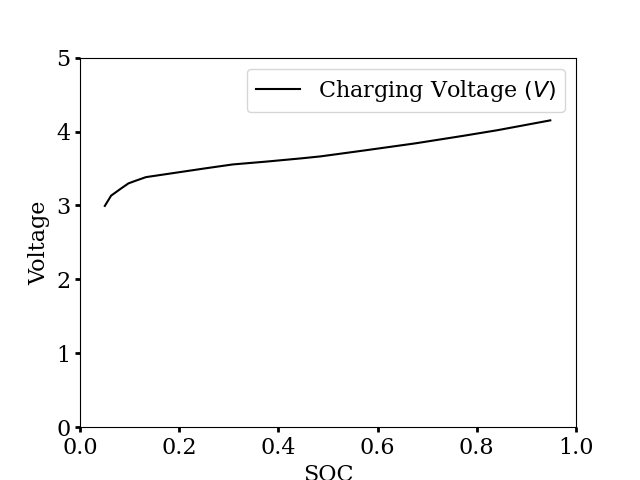
\includegraphics[scale=.4]{Chap06/Figures/PowerAnalyzerResults/Batt_Charging_Voltage_SOC.png}}
	\qquad
	\subfigure[MIFA]{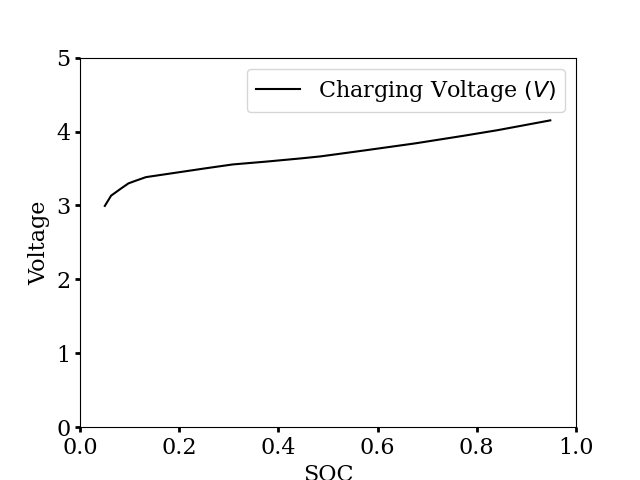
\includegraphics[scale=.4]{Chap06/Figures/PowerAnalyzerResults/Batt_Charging_Voltage_SOC.png}}
	\caption{MIFA Antenna Gain Radiation Pattren}
\end{figure}

% \begin{tikzpicture}
%     \begin{axis}[legend entries={ChvBatt0},
%     %legend style={
%     %at={(0.5,-0.2)},
%     %anchor=north,
%     %legend columns=1,
%     %cells={anchor=west},
%     %font=\footnotesize,
%     %rounded corners=2pt,
%     %}, 
%     \addplot table [x=Index, y=ChvBatt0, col sep=comma] {Chap06/Code/Batt.csv};

%     \end{axis}
% \end{tikzpicture}